\RequirePackage{pdf14}
\documentclass[pdfa]{drdc-report}
\usepackage{drdc-docctl}
\usepackage{drdc-rtf-abstract}
\usepackage{drdc-submission}

% Use T1 fonts for correct French hyphenation
\usepackage[T1]{fontenc}
\usepackage[utf8]{inputenc}
\usepackage{lmodern}
\renewcommand\sfdefault{phv}
\usepackage{glossaries}
\usepackage{amsbsy}
\usepackage{amsmath}
\usepackage{amsthm}
% \ifx\pdftexversion\undefined
%   \usepackage[dvips]{graphicx}
% \else
%   \usepackage[pdftex]{graphicx,hyperref}
%   \hypersetup{backref,colorlinks=true,plainpages=false,pdfpagelabels}
%   \hypersetup{%
%     colorlinks=true,   % aktiviert farbige Referenzen
%     linkcolor=black,    % Make the link colours blue
%     citecolor=black,
%     filecolor=black,
%     pdfpagemode=UseNone,  % PDF-Viewer startet ohne Inhaltsverzeichnis et.al.
%     pdfstartview=FitH} % PDF-Viewer benutzt beim Start bestimmte Seitenbreite
%   
%   \hypersetup{% Ä=\304; Ö=\326; Ü=\334; ä=\344; ö=\366; ü=\374; ß=\377
%     pdftitle={Wavenumber domain representation of satellite signal},
%     pdfauthor={Ishuwa C. Sikaneta},
%     pdfsubject={Special Functions},
%     pdfkeywords={Statistics, Product model, Stationarity, Gaussian, Non Gaussian, SAR, GMTI, CFAR}
%   }
% \fi
% \usepackage[x11names, svgnames, rgb]{xcolor}
%\usepackage[utf8]{inputenc}
\usepackage{tikz}
\usepackage{pgfplots}
\usetikzlibrary{snakes,arrows,shapes}

\usepackage[mathscr]{euscript}
\usepackage{subcaption}
\usepackage{dblfloatfix}
\usepackage{fixltx2e}
\usepackage{color}
\usepackage{array, hhline}
\usepackage[normalem]{ulem}
\usepackage{rotating}
\usepackage{marvosym}
\usepackage{multirow}
\usepackage[mathscr]{euscript}
\usepackage{listings}
% \definecolor{gray}{rgb}{0.4,0.4,0.4}
% \definecolor{darkblue}{rgb}{0.0,0.0,0.6}
% \definecolor{cyan}{rgb}{0.0,0.6,0.6}
% \definecolor{Brown}{cmyk}{0,0.81,1,0.60}
% \definecolor{OliveGreen}{cmyk}{0.64,0,0.95,0.40}
% \definecolor{CadetBlue}{cmyk}{0.62,0.57,0.23,0}

\definecolor{lightlightgray}{gray}{0.9}
\definecolor{dkgreen}{rgb}{0,0.6,0}
\definecolor{gray}{rgb}{0.5,0.5,0.5}
\definecolor{mauve}{rgb}{0.58,0,0.82}
\definecolor{gray}{rgb}{0.4,0.4,0.4}
\definecolor{darkblue}{rgb}{0.0,0.0,0.6}
\definecolor{lightblue}{rgb}{0.0,0.0,0.9}
\definecolor{cyan}{rgb}{0.0,0.6,0.6}
\definecolor{darkred}{rgb}{0.6,0.0,0.0}


\lstset{
  basicstyle=\ttfamily\footnotesize,
  columns=fullflexible,
  showstringspaces=false,
  numbers=left,                                % where to put the line-numbers
  numberstyle=\tiny\color{gray},               % the style that is used for the line-numbers
  stepnumber=1,
  numbersep=5pt,                               % how far the line-numbers are from the code
  backgroundcolor=\color{lightlightgray},      % choose the background color. You must add \usepackage{color}
  showspaces=false,                            % show spaces adding particular underscores
  showstringspaces=false,                      % underline spaces within strings
  showtabs=false,                              % show tabs within strings adding particular underscores
  frame=none,                                  % adds a frame around the code
  rulecolor=\color{black},                     % if not set, the frame-color may be changed on line-breaks within not-black text (e.g. commens (green here))
  tabsize=2,                                   % sets default tabsize to 2 spaces
  captionpos=b,                                % sets the caption-position to bottom
  breaklines=true,                             % sets automatic line breaking
  breakatwhitespace=false,                     % sets if automatic breaks should only happen at whitespace
  title=\lstname,                              % show the filename of files included with \lstinputlisting;
                                               % also try caption instead of title  
  commentstyle=\color{gray}\upshape
}


\lstdefinelanguage{XML}
{
  morestring=[s][\color{mauve}]{"}{"},
  morestring=[s][\color{black}]{>}{<},
  morecomment=[s]{<?}{?>},
  morecomment=[s][\color{dkgreen}]{<!--}{-->},
  stringstyle=\color{black},
  identifierstyle=\color{lightblue},
  keywordstyle=\color{red},
  morekeywords={xmlns,xsi,noNamespaceSchemaLocation,type,id,x,y,source,target,version,tool,transRef,roleRef,objective,eventually}% list your attributes here
}


\usepackage[bibstyle=nature, style=numeric, citestyle=numeric-comp, sorting=none, backend=biber]{biblatex}
\bibliography{/home/ishuwa/Documents/bibliography/ishbib}
% \usepackage[style=numeric, citestyle=numeric-comp, sorting=none, backend=biber]{biblatex}

% Load hyperref
\definecolor{navy}{rgb}{0,0,0.5}
\definecolor{Maroon}{rgb}{0.6836,0.1953,0.2070}
\newcommand\mydriver{\ifpdf pdftex\else dvips,breaklinks\fi}
\usepackage[\mydriver,draft=false,plainpages=false,
    colorlinks=true,linkcolor=navy,anchorcolor=navy,citecolor=navy,
    filecolor=navy,urlcolor=navy,raiselinks=true,
    bookmarksnumbered=true]{hyperref}

\newcommand\mytitle{Super Resolution Synthetic Aperture Radar}
\title{\mytitle}
\subtitle{Design and Signal Processing of a Multi-Beam Multi-Channel Stripmap Mode}
\docnumber{---Will be inserted by Publication Officer}
\establishment{\DRDCO}
%\author{C.H.~Gierull}
\author{I.C. Sikaneta}
\authors{I.C.~Sikaneta[International Atomic Energy Agency - Vienna]
         C.H.~Gierull[\establishmentname]%
         }

% These definitions are used by drdc-docctl.sty
\projectnumber{42zz78}
\addkeyword{SAR}
\addkeyword{HRWS}
\addkeyword{Multi-channel}
\addkeyword{Orbit}
\addkeyword{Differential geometry}
\addkeyword{Multi-beam}
\addkeyword{Spherical harmonics}
\addkeyword{High-resolution}
\addkeyword{Phased-array}
\addkeyword{True time-delay}
\addkeyword{Spotlight}

% Pass title, author and keywords to hyperref to put in the PDF Info.
\makeinitializedauthors\mypdfauthors{; }
\makeexpandedkeywords\mypdfkeywords{; }
\hypersetup{
  pdftitle={\mytitle},
  pdfauthor={\mypdfauthors},
  pdfkeywords={\mypdfkeywords}
}
\futuredistribution{Defence departments and their contractors}{None}

%Public release
%Defence departments
%Defence departments and their contractors
%Government departments/agencies
%Government departments/agencies and their contractors
%Further distribution done by approval from Defence Research and Development Canada’s Authority

%\distribution
\newcommand{\vct}[1]{\ensuremath{\mathbf{#1}}}                                                    
\newcommand{\mtx}[1]{\ensuremath{\mathbf{\uppercase{#1}}}}                                   
\newcommand{\htr}[1]{\ensuremath{#1^\dagger}}
\newcommand{\dtm}[1]{\ensuremath{\lvert #1\rvert}}   
\newcommand{\im}{\ensuremath{i}}
\newcommand{\vhat}[1]{\ensuremath{\hat{\mathbf{#1}}}}

%\newcommand{\vre}{\ensuremath{v_{\vct{\xi}}}}

% Section, figure, table and equation references
\renewcommand{\eqref}[1]{(\ref{#1})}                                                    % equation reference
\newcommand{\Eqref}[1]{{Equation (\ref{#1})}}                                                      % Equation reference
\newcommand{\fgref}[1]{{Figure \ref{#1}}}                                                        % figure reference
\newcommand{\Fgref}[1]{{Figure \ref{#1}}}                                                        % Figure reference
\newcommand{\tbref}[1]{Table \ref{#1}}                                                               % table reference
\newcommand{\Tbref}[1]{Table \ref{#1}}                                                               % Table reference
\newcommand{\cpref}[1]{Chapter \ref{#1}}                                                             % chapter reference
\newcommand{\Cpref}[1]{Chapter \ref{#1}}                                                             % Chapter reference
\newcommand{\anref}[1]{{Appendix \ref{#1}}}                                                      % appendix reference
\newcommand{\Anref}[1]{{Appendix \ref{#1}}}                                                      % Appendix reference
\newcommand{\scref}[1]{{Section \ref{#1}}}                                                       % section reference
\newcommand{\Scref}[1]{{Section \ref{#1}}}                                                       % Section reference
\newcommand{\lmref}[1]{{Lemma \ref{#1}}}                                                       % lemma reference
\newcommand{\Lmref}[1]{{Lemma \ref{#1}}}                                                       % lemma reference

% Expected value
\newcommand{\expct}[1]{\ensuremath{\mathcal{E}\{#1\}}}                                          
\newcommand{\Expct}[1]{\ensuremath{\mathcal{E}\biggl\{#1\biggr\}}}  
\newcommand{\eex}[1]{\ensuremath{e^{#1}}}                                     
\newcommand{\ex}[1]{\ensuremath{\exp(#1)}}
\newcommand{\Ex}[1]{\ensuremath{\exp\biggl(#1\biggr)}}

\newcommand{\fdc}{\ensuremath{f_{\parm_{dc}}}}
\newcommand{\mtxIdentity}{\ensuremath{\mtx{I}}}

\newcommand{\pulse}{\ensuremath{z}}
\newcommand{\Pulse}{\ensuremath{Z}}
\newcommand{\envelope}{\ensuremath{p}}
\newcommand{\Envelope}{\ensuremath{P}}
\newcommand{\Snvelope}{\ensuremath{\mathscr{P}}}
\newcommand{\snvelope}{\ensuremath{\text{p}}}
\newcommand{\range}{\ensuremath{r}}
\newcommand{\rangeError}{\ensuremath{\delta_\range}}
\newcommand{\rangeErrorZero}{\ensuremath{\delta_{\range_0}}}
\newcommand{\stolt}{\ensuremath{\psi}}
\newcommand{\velocity}{\ensuremath{v}}
\newcommand{\acceleration}{\ensuremath{a}}
\newcommand{\sat}{\ensuremath{\vct{c}}}
\newcommand{\target}{\ensuremath{\vct{x}}}
\renewcommand{\d}{\ensuremath{\text{d}}}
\newcommand{\parm}{\ensuremath{s}}
\newcommand{\tparm}{\ensuremath{t}}
\newcommand{\fasttime}{\ensuremath{\tau}}
\newcommand{\satparm}{\ensuremath{\vct\sat(\parm)}}
\newcommand{\targetnoparm}{\ensuremath{\vct\target}}
\newcommand{\targetnoparmzero}{\ensuremath{\vct{x}_0}}
\newcommand{\uSatVelocity}[1]{\ensuremath{\vhat\velocity_\sat(#1)}}
\newcommand{\huSatVelocity}[1]{\ensuremath{\htr{\vhat\velocity}_\sat(#1)}}
\newcommand{\satVelocity}[1]{\ensuremath{\vct\velocity_\sat(#1)}}
\newcommand{\vtarget}{\ensuremath{\vct\velocity_\target}}
\newcommand{\hsatVelocity}[1]{\ensuremath{\htr{\vct\velocity}_\sat(#1)}}
\newcommand{\rcoeff}{\ensuremath{a}}

\newcommand{\targetVelocity}[1]{\ensuremath{\vct\velocity^\stationarySymbol_t(#1)}}
\newcommand{\rangeVectorParm}{\ensuremath{\vct{\range}(\parm, \targetnoparm)}}
\newcommand{\defrangeVectorParmZero}{\ensuremath{\vct{\range}(\parm_0, \targetnoparm_0)}}
\newcommand{\rangeVectorParmZero}{\ensuremath{\vct{\range}_0}}
\newcommand{\rangeVector}[1]{\ensuremath{\vct\range(#1)}}
\newcommand{\hrangeVector}[1]{\ensuremath{\htr{\vct\range}(#1)}}
\newcommand{\uRangeVectorParm}{\ensuremath{\vhat{\range}(\parm, \targetnoparm)}}
\newcommand{\defuRangeVectorParmZero}{\ensuremath{\vhat{\range}(\parm_0, \targetnoparm_0)}}
\newcommand{\uRangeVectorParmZero}{\ensuremath{\vhat{\range}_0}}
\newcommand{\uRangeVectorParmZeroPerp}{\ensuremath{\vhat{\range}_{0\bot}}}
\newcommand{\huRangeVectorParm}{\ensuremath{\htr{\vhat{\range}}(\parm)}}
\newcommand{\RangeVector}[1]{\ensuremath{\vct\range(#1)}}
\newcommand{\hRangeVector}[1]{\ensuremath{\htr{\vct\range}(#1)}}
\newcommand{\lat}{\ensuremath{\phi}_s}
\newcommand{\lng}{\ensuremath{\lambda}_s}
\newcommand{\rresolution}{\ensuremath{\delta_\range}}

\newcommand{\uRangeVector}[1]{\ensuremath{\vhat{\range}(#1)}}
\newcommand{\uRangeVectorl}[2]{\ensuremath{\vhat{\range}_{#1}(#2)}}
\newcommand{\huRangeVector}[1]{\ensuremath{\htr{\vhat{\range}}(#1)}}
\newcommand{\huRangeVectorl}[2]{\ensuremath{\htr{\vhat{\range}_{#1}}(#2)}}
\newcommand{\antennaPosition}[1]{\ensuremath{\vct{p}_{#1}}}
\newcommand{\pAntennaParm}[1]{\ensuremath{\vct{p}_{#1}(\parm)}}
\newcommand{\pAntennaParms}[1]{\ensuremath{\vct{p}_{#1}(\parm_s)}}
\newcommand{\pAntenna}[2]{\ensuremath{\vct{p}_{#1}(#2)}}
\newcommand{\xAntennaNoParm}[1]{\ensuremath{\vct{p}_{#1}}}
\newcommand{\xAntenna}[2]{\ensuremath{\xAntennaNoParm{#1}(#2)}}
\newcommand{\kr}{\ensuremath{k_r}}
\newcommand{\krn}{\ensuremath{k_{r'}}}
\newcommand{\krstolt}{\ensuremath{k_{r_s}}}
\newcommand{\krc}{\ensuremath{\krn}}
\newcommand{\krnaught}{\ensuremath{k_{r_0}}}
\renewcommand{\r}{\ensuremath{r_0}}
\newcommand{\xparm}{\ensuremath{\parm}}
\newcommand{\stationaryparm}{\ensuremath{\parm_p}}
\newcommand{\kparm}{\ensuremath{k_{\xparm}}}
\newcommand{\kparmPRF}{\ensuremath{k_{\xparm_p}}}
\newcommand{\gfunc}{\ensuremath{g}}
\newcommand{\myparm}{\ensuremath{\parm^*}}

% Signal in different domains
\newcommand{\ztzt}[1]{\ensuremath{zz_{#1}}}
\newcommand{\stst}[1]{\ensuremath{ss_{#1}}}
\newcommand{\Sfst}[1]{\ensuremath{Ss_{#1}}}
\newcommand{\SfSf}[1]{\ensuremath{SS_{#1}}}
\newcommand{\Skst}[1]{\ensuremath{\mathscr{S}s_{#1}}}
\newcommand{\SkSf}[1]{\ensuremath{\mathscr{S}S_{#1}}}
\newcommand{\SkSk}[1]{\ensuremath{\mathscr{S}\mathscr{S}_{#1}}}
\newcommand{\srSk}[1]{\ensuremath{s\mathscr{S}_{#1}}}
\newcommand{\SkSkM}{\ensuremath{\mtx{S}}}
\newcommand{\ststV}{\ensuremath{\boldsymbol{s}\boldsymbol{s}}}
\newcommand{\SfstV}{\ensuremath{\boldsymbol{S}\boldsymbol{s}}}
\newcommand{\SkstV}{\ensuremath{\boldsymbol{\mathscr{S}}\boldsymbol{s}}}
\newcommand{\SkSkV}{\ensuremath{\vct{s}}}
\newcommand{\SkSfV}{\ensuremath{\boldsymbol{\mathscr{S}}\boldsymbol{S}}}
\newcommand{\ZkZkM}{\ensuremath{\vct{z}}}
\newcommand{\SkSkR}{\ensuremath{\mathscr{S}\mathscr{S}_{R}}}
\newcommand{\ZkZkR}{\ensuremath{\mathscr{Z}\mathscr{Z}_{R}}}
\newcommand{\NkNkM}{\ensuremath{\vct{n}}}
\newcommand{\NkNkMP}{\ensuremath{\boldsymbol{\nu}}}

\newcommand{\fparm}{\ensuremath{f_\parm}}
\newcommand{\fparmPRF}{\ensuremath{f_{\parm_p}}}
\newcommand{\rangepos}{\ensuremath{\vct\range}_0}
\newcommand{\uRangepos}{\ensuremath{\vhat{\range}}_0}
\newcommand{\rangevel}{\ensuremath{{\vct{\velocity}}}_0}
\newcommand{\uRangevel}{\ensuremath{{\vhat{\velocity}}}_0}
\newcommand{\rangeacc}{\ensuremath{{\vct{\acceleration}}}_0}
\newcommand{\channelIndex}{\ensuremath{n}}
\newcommand{\beamIndex}{\ensuremath{m}}
\newcommand{\pattern}[1]{\ensuremath{\text{A}_{#1}}}
\newcommand{\dPattern}[1]{\ensuremath{\text{D}_{#1}}}
\newcommand{\dazPattern}[1]{\ensuremath{\text{D}_{\text{az}_{#1}}}}
\newcommand{\delPattern}[1]{\ensuremath{\text{D}_{\text{el}_{#1}}}}
\newcommand{\dconstelPattern}{\ensuremath{\text{D}_{\text{el}}}}
\newcommand{\edPattern}[1]{\ensuremath{\text{E}_{#1}}}
\newcommand{\elementPattern}[1]{\ensuremath{\text{E}_{#1}}}
\newcommand{\magVec}[1]{\ensuremath{\lvert#1\rvert}}
\newcommand{\amplitude}[1]{\ensuremath{\mathnormal{#1}}}
\newcommand{\Tx}[1]{\ensuremath{\vct\target\text{\footnotesize{x}}_{#1}}}
\newcommand{\Rx}[1]{\ensuremath{\vct\range\text{\footnotesize{x}}_{#1}}}
\newcommand{\costFunction}[1]{\ensuremath{J}_{#1}}
\newcommand{\eVec}[1]{\ensuremath{\vct{e}_{#1}}}
\newcommand{\heVec}[1]{\ensuremath{\htr{\vct{e}}_{#1}}}
\newcommand{\ebVec}[1]{\ensuremath{\vct{b}_{#1}}}
\newcommand{\hbVec}[1]{\ensuremath{\htr{\vct{b}}_{#1}}}
\newcommand{\cost}{\ensuremath{\varrho}}
\newcommand{\kvec}{\ensuremath{\vct{k}}}
\newcommand{\kveczero}{\ensuremath{\kr, \kparm}}
\newcommand{\kvecl}{\ensuremath{\kr, \kparm + l\kparmPRF}}
\newcommand{\kargs}{\ensuremath{\kr,\kparm}}
\newcommand{\hkvec}{\ensuremath{\htr{\vct{k}}}}
\newcommand{\effrelvel}{\ensuremath{\velocity_e}}
\newcommand{\vsat}{\ensuremath{\velocity_\sat}}
\newcommand{\transmitSet}[1]{\ensuremath{\mathcal{T}_{#1}}}
\newcommand{\arrayVector}{\ensuremath{\vct{e}}}
\newcommand{\transmitVector}[1]{\ensuremath{\vct{T}_{x_{#1}}}}
\newcommand{\htransmitVector}[1]{\ensuremath{\htr{\vct{T}}_{x_{#1}}}}
\newcommand{\receiveVector}[1]{\ensuremath{\vct{R}_{x_{#1}}}}
\newcommand{\hreceiveVector}[1]{\ensuremath{\htr{\vct{R}}_{x_{#1}}}}
\newcommand{\receiveSet}[1]{\ensuremath{\mathcal{R}_{#1}}}
\newcommand{\spacing}{\ensuremath{d}}
\newcommand{\nadAngle}{\ensuremath{\phi_0}}
\newcommand{\numberChannels}{\ensuremath{N_c}}
\newcommand{\channelM}{\ensuremath{M}}
\newcommand{\uX}[1]{\ensuremath{\vct{\hat{x}}(#1)}}
\newcommand{\uY}[1]{\ensuremath{\vct{\hat{y}}(#1)}}
\newcommand{\uZ}[1]{\ensuremath{\vct{\hat{z}}(#1)}}

\newcommand{\targetx}{\ensuremath{x}}
\newcommand{\targety}{\ensuremath{y}}
\newcommand{\targetz}{\ensuremath{z}}
\newcommand{\squint}{\ensuremath{\vartheta_s}}

\newcommand{\re}{\ensuremath{r_e}}
\newcommand{\rs}{\ensuremath{r_s}}
\newcommand{\rxz}{\ensuremath{r_{xz}}}
\newcommand{\rxy}{\ensuremath{r_{xy}}}
\newcommand{\rzy}{\ensuremath{r_z}}
\newcommand{\omegas}{\ensuremath{\omega_s}}
\newcommand{\satECEFangular}{\ensuremath{\boldsymbol\omega}_\sat}
\newcommand{\angular}{\ensuremath{\hat{\boldsymbol\omega}_\sat}}
\newcommand{\depression}{\ensuremath{\phi}}
\newcommand{\targetdepression}{\ensuremath{\depression}}
\newcommand{\targetomega}{\ensuremath{\omegas\parm_0}}
\newcommand{\targetrange}{\ensuremath{\range}}
\newcommand{\targetxparm}{\ensuremath{\xparm_{\target}}}
\newcommand{\targetrangez}{\ensuremath{\range_0}}
\newcommand{\targetxparmz}{\ensuremath{\xparm_{t_0}}}
\newcommand{\targetdepressionz}{\ensuremath{\depression_{0}}}
\newcommand{\omegat}{\ensuremath{\omega_t}}
\newcommand{\thetat}{\ensuremath{\theta_0}}
\newcommand{\thetas}{\ensuremath{\theta_s}}
\newcommand{\Thetas}{\ensuremath{\Theta_s}}
\newcommand{\phaser}{\ensuremath{\Psi_r}}
\newcommand{\alongtrack}{\ensuremath{{\alpha_\parallel}_n}}
\newcommand{\alongtrackparm}[1]{\ensuremath{{\alpha_\parallel}_{#1}}}
\newcommand{\acrosstrack}{\ensuremath{{\boldsymbol{\alpha}_\perp}_n}}

\newcommand{\antennaVector}{\ensuremath{\vct{a}}}
\newcommand{\antennaMatrix}{\ensuremath{\mtx{H}}}
\newcommand{\antennaPhaseMatrix}{\ensuremath{\mtx{P}}}
\newcommand{\diagAntennaMatrix}{\ensuremath{\mtx{D}}}
\newcommand{\hrwsFilterMatrix}{\ensuremath{\mtx{B}}}
\newcommand{\anTx}[1]{\ensuremath{\vct{T}_{x_{#1}}}}
\newcommand{\anRx}[1]{\ensuremath{\vct{R}_{x_{#1}}}}
\newcommand{\txDelay}[1]{\ensuremath{\delta_{T_{#1}}}}
\newcommand{\rxDelay}[1]{\ensuremath{\delta_{R_{#1}}}}
\newcommand{\txAmp}[1]{\ensuremath{\text{A}_{T_{#1}}}}
\newcommand{\rxAmp}[1]{\ensuremath{\text{A}_{R_{#1}}}}
\newcommand{\bline}{\ensuremath{\vct{b}}}
\newcommand{\uzero}{\ensuremath{\vct{u}_\channelIndex}}
\newcommand{\txn}{\ensuremath{n'}}
\newcommand{\txm}{\ensuremath{m'}}
\newcommand{\txN}{\ensuremath{N'}}
\newcommand{\txM}{\ensuremath{M'}}
\newcommand{\mnDelay}{\ensuremath{\delta_{\txm\txn}}}
\newcommand{\xang}{\ensuremath{x}}
\newcommand{\shelp}[3]{\ensuremath{\psi(\xang;#1,#2,#3)}}

\newcommand{\dthetas}{\ensuremath{\dot\theta_s}}
\newcommand{\gweight}[1]{\ensuremath{D_{#1}}}
\newcommand{\hgweight}[1]{\ensuremath{\averageAntenna^*_{#1}}}
\newcommand{\reflectivity}{\ensuremath{g}}
\newcommand{\vkern}{\ensuremath{\varPhi}}
\newcommand{\vkernvect}{\ensuremath{\boldsymbol{\vkern}}}
\newcommand{\alphaSymbol}{\ensuremath{\alpha}}
\newcommand{\betaSymbol}{\ensuremath{\beta}}
\newcommand{\gammaSymbol}{\ensuremath{\gamma}}
\newcommand{\alphaComponent}[1]{\ensuremath{\alphaSymbol_{#1}}}
\newcommand{\betaComponent}[1]{\ensuremath{\betaSymbol_{#1}}}
\newcommand{\gammaComponent}[1]{\ensuremath{\gammaSymbol_{#1}}}

\newcommand{\ct}{\ensuremath{\cos\omega_e t}}
\newcommand{\st}{\ensuremath{\sin\omega_e t}}
\newcommand{\del}{\ensuremath{\vec{\nabla}}}
\newcommand{\grad}{\ensuremath{\Delta}}
\newcommand{\Pf}{\ensuremath{\mtx{P}_\vct{f}}}
\newcommand{\uf}{\ensuremath{\hat{\vct{f}}}}
\newcommand{\df}{\ensuremath{\dot{\vct{f}}}}
\newcommand{\sats}{\ensuremath{\vct{c}_s}}
\newcommand{\satp}{\ensuremath{\vct{c}_p}}
\newcommand{\satt}{\ensuremath{\vct{c}_t}}
\newcommand{\dx}{\ensuremath{\dot{\satt}}}
\newcommand{\dw}{\ensuremath{\dot{\vct{w}}}}
\newcommand{\uw}{\ensuremath{\hat{\vct{w}}}}
\newcommand{\ddx}{\ensuremath{\ddot{\satt}}}
\newcommand{\udx}{\ensuremath{\hat{\dot{\satt}}}}
\newcommand{\dddx}{\ensuremath{\dddot{\satt}}}
\newcommand{\Px}{\ensuremath{\mtx{P}_{\satt}}}
\newcommand{\Pdx}{\ensuremath{\mtx{P}_{\dx(t)}}}
\newcommand{\Itwo}{\ensuremath{\mtx{I}_2}}
\newcommand{\Qtwo}{\ensuremath{\mtx{Q}_2}}
\newcommand{\prt}[2]{\ensuremath{\frac{\partial #1}{\partial #2}}}
\newcommand{\dtv}[2]{\ensuremath{\frac{\text{d}#1}{\text{d}#2}}}
\newcommand{\dtvtwo}[2]{\ensuremath{\frac{\text{d}^2#1}{\text{d}#2^2}}}
\newcommand{\dtvthree}[2]{\ensuremath{\frac{\text{d}^3#1}{\text{d}#2^3}}}
\newcommand{\prttwoa}[2]{\ensuremath{\frac{\partial^2#1}{\partial#2^2}}}
\newcommand{\prttwob}[3]{\ensuremath{\frac{\partial^2#1}{\partial#2\partial#3}}}

%\newcommand{\satparm}{\ensuremath{\vct{c}(s)}}
%\newcommand{\target}{\ensuremath{\vct{P}}}
\newcommand\Index[1]{#1}
\newcommand{\gls}[1]{#1}

\newcommand{\prf}{\ensuremath{f_p}}
\newcommand{\antennaLength}{\ensuremath{L}}
\newcommand{\antennaLengthDesired}{\ensuremath{L_0}}
\newcommand{\antennaLengthEffective}{\ensuremath{L_M}}
\newcommand{\wavelength}{\ensuremath{\lambda}}

% Input from SURE.tex
\newcommand{\threeDB}{\ensuremath{\Theta}}
\newcommand{\threeDBDesired}{\ensuremath{\Theta_{0}}}
\newcommand{\threeDBEffective}{\ensuremath{\Theta_{M}}}
\newcommand{\satv}{\ensuremath{v_s}}
\newcommand{\aziBW}{\ensuremath{B_a}}
\newcommand{\aziRes}{\ensuremath{\delta_x}}
\newcommand{\prfEffective}{\ensuremath{\prf}}
\newcommand{\prfreal}{\ensuremath{f_M}}
\newcommand{\resxDesired}{\ensuremath{\delta_0}}
\newcommand{\phaseSep}{\ensuremath{d}}
\newcommand{\lookdirection}{\ensuremath{\hat{u}}}
\newcommand{\vecsigTime}{\ensuremath{\vct{z}}}
\newcommand{\vecsigFreq}{\ensuremath{\vct{Z}}}
\newcommand{\vecsigFreqSampled}{\ensuremath{\vct{Z}_s}}
\newcommand{\htrvecsigFreqSampled}{\ensuremath{\htr{\vct{Z}}_s}}
\newcommand{\phaseCentreLocation}[1]{\ensuremath{\vct{p}_{#1}}}
\newcommand{\temporalbaseline}{\ensuremath{d_t}}
\newcommand{\spatialbaseline}{\ensuremath{d_s}}
\newcommand{\opt}{\rm opt}
\newcommand{\weight}[1]{\ensuremath{z_{#1}}}
\newcommand{\Nbands}{\ensuremath{N_{b}}}
\newcommand{\costweight}{\ensuremath{\varrho}}
\newcommand{\winweight}[1]{\ensuremath{\zeta_{#1}}}
\newcommand{\Winweight}{\ensuremath{\boldsymbol{\zeta}}}
\newcommand{\vopt}[1]{\ensuremath{\vct{v}^{\cg{\opt}}_{#1}}}
\newcommand{\Vopt}{\ensuremath{\mtx{V}_{\cg{\opt}}}}
\newcommand{\eigval}[1]{\ensuremath{\lambda_{#1}}}
\newcommand{\eigvec}[1]{\ensuremath{\vct{u}_{#1}}}
\newcommand{\alert}[1]{\textcolor{blue}{#1}}
\newcommand{\ish}[1]{\textcolor{blue}{#1}}
\newcommand{\cg}[1]{{#1}}
\newcommand{\cgs}[1]{\textcolor{red}{\sout{#1}}}
% \newcommand{\ishfix}[3]{{\textcolor{cyan}{#1}}{\tiny\textcolor{magenta}{#2}}{\scshape\small\textcolor{red}{#3}}}
\newcommand{\ishfix}[3]{#1}
\newcommand{\figref}[1]{\figurename~\ref{#1}}
\newtheorem{theorem}{Theorem}[section]
\newtheorem{corollary}{Corollary}[section]
\newtheorem{lemma}{Lemma}[section]
\newtheorem{question}{Question}[section]
\newtheorem{Definition}{Definition}[section]
\newcommand{\figD}{\ensuremath{\phaseSep=M\resxDesired=11\resxDesired}}
\newcommand{\figL}{\ensuremath{\antennaLengthEffective=2M\resxDesired=22\resxDesired}}
\newcommand{\figWL}{\ensuremath{\antennaLength=2M^2\resxDesired=242\resxDesired}}
\newcommand{\carrier}{\ensuremath{f_0}}

\newacronym{snr}{SNR}{Signal to Noise Ratio}
\newacronym{sar}{SAR}{Synthetic Aperture Radar}
\newacronym{gmti}{GMTI}{Ground Moving Target Indication}
\newacronym{mti}{MTI}{Moving Target Indication}
\newacronym{hrws}{HRWS}{High-Resolution, Wide-Swath}
\newacronym{psf}{PSF}{Point Spread Function}
\newacronym{cfar}{CFAR}{Constant False Alarm Rate}
\newacronym{prf}{PRF}{Pulse Repetition Frequency}
\newacronym{pri}{PRI}{Pulse Repetition Interval}
\newacronym{mmse}{MMSE}{Minimum Mean Square Error}
\newacronym{ecef}{ECEF}{Earth-Centered, Earth-Fixed}
\newacronym{dpca}{DPCA}{Displaced Phase Centre Antenna}
\newacronym{dra}{DRA}{Dual-receive aperture}
\newacronym{ft}{FT}{Fourier Transform}
\newacronym{dlr}{DLR}{Deutsches zentrum f\"ur Luft- und Raumfahrt}
\newacronym{leo}{LEO}{Low-Earth Orbit}

% Glossary entries
\newglossaryentry{parr}{name={phased-array},description={An array of identical antennas all on the same clock usually uniformly spaced}}
\newglossaryentry{stripmap}{name={Stripmap mode}, description={Standard SAR imaging mode with medium area coverage and medium resolution}}
\newglossaryentry{spotlight}{name={Spotlight mode}, description={High=resolution SAR imaging mode with small area coverage}}
\newglossaryentry{scansar}{name={ScanSAR mode}, description={Low-resolution multi-elevation-beam SAR imaging mode for wide-area coverage}}
\newglossaryentry{adiv}{name={Antenna diversity}, description={A multiplicity of radar antennas}}
\newglossaryentry{acint}{name={Across-track interferometry}, description={Interferometry with an across-track baseline. Used for creating digital elevation models or subsidence maps}}
\newglossaryentry{rs2}{name={RADARSAT-2}, description={Canadian commercial C-band SAR}}
\newglossaryentry{alp2}{name={ALOS PALSAR-2}, description={Japanese commercial L-band SAR}}
\newglossaryentry{tsx}{name={TerraSAR-X}, description={German commercial X-band SAR}}
\newglossaryentry{yaw}{name={yaw-steering}, description={Space-based radar platfrom yaw-steering method to align the antenna with its track in an ECEF coordinate system}}
\newglossaryentry{tzd}{name={total zero-Doppler steering}, description={Space-based radar platfrom yaw and pitch steering method to ensure that the antenna is totally aligned with its track in an ECEF coordinate system}}
\newglossaryentry{clutter}{name={clutter}, description={The radar return from scatterers on the terrain that are not the target of interest}}
\newglossaryentry{wideband}{name={wideband}, description={A signal where the bandwidth to centre frequency ratio is large. For these signals, the wavelength cannot be approximated as constant}}
\newglossaryentry{narrowband}{name={narrowband}, description={A signal where the bandwidth to centre frequency ratio is small. For these signals, the wavelength can be approximated as constant}}
\newglossaryentry{spacetime}{name={Space-time sampling diagram}, description={A scatter plot showing the antenna phase-centre spatial locations as a function of time}}
\newglossaryentry{dpcacondition}{name={DPCA Condition}, description={A combination of PRF and along-track baseline such that all antennas measure from the same point in space at different times}}
\newglossaryentry{antidpcacondition}{name={anti-DPCA}, description={A combination of PRF and along-track baseline which achieves uniform spatial sampling with each point sampled only once}}
\newglossaryentry{widefine}{name={widefine}, description={A dual-receive RADARSAT-2 imaging mode}}
\newglossaryentry{ultrafine}{name={ultrafine}, description={A dual-receive RADARSAT-2 imaging mode}}
\newglossaryentry{interleave}{name={interleave}, description={Samples from multiple channels are arranged according to sampling time in a new sequence}}
\newglossaryentry{dopcen}{name={Doppler centroid}, description={The Doppler frequency corresponding to the azimuth angle on which the azimuth antenna is centred}}
\newglossaryentry{stolt}{name={Stolt interpolation}, description={2-D interpolation prescription at the core of the wavenumber SAR processing algorithm}}
\newglossaryentry{spa}{name={stationary phase approximation}, description={Procedure for approximating certain types of integrals}}

\DeclareUnicodeCharacter{2212}{-}
\pgfplotsset{compat=1.16}

\begin{document}

% Add the cover page
\makefrontcover

\begin{abstract}
By presenting the design, configuration and required end-to-end signal processing, this report proposes a system for improved \Index{\gls{sar}} imaging. Compared to conventional Spotlight \gls{sar}, the proposed system will generate imagery with equivalent or better resolution and significantly increased area coverage. The design and configuration are based upon a phased-array antenna in combination with the appropriate hardware to enable rapid electronic beam steering and to permit digitisation of multiple receive channels. The current state of technology is mature enough to construct all components of such a system. As a specific goal, the report proposes a system capable of imaging with 10 cm resolution (azimuth and slant-range) over a ground swath of 5 km. The proposed system is simulated at X-band, but could, in principle, be operated at any band with sufficiently available bandwidth. Importantly, this mode can collect with unlimited azimuth extent, something that no other proposed system can achieve.
\par
As the considered resolutions push the limits of known theory, the report also introduces an augmented theory that is needed to derive the signal processing algorithms. The presented approach incorporates a physical model, based upon the spherical harmonic model of the Earth's gravitational potential, into the theory of differential geometry of curves in three dimensions. From the theory, a wavenumber-based \gls{sar} processing algorithm that extends current methods is developed and presented. The proposed algorithm relies only on accurate attitude data and a single accurate state vector. The approach is therefore suitable for on-board SAR processing if sensor instruments can measure these parameters while imaging.
\end{abstract}

\begin{significance}
The material presented in this report provides the design and signal-processing framework for a \gls{sar} that can image with extremely high resolutions over wide areas. This capability does not exist for current systems, nor will it be possible with future systems, as currently planned. On the one hand, the novel proposed design offers improved SAR imaging without giving up any of the capabilities currently offered by national assets. On the other hand, the improvements meet or exceed current capability gaps in C4ISR requirements. The design (or some variant thereof) should be considered for future \gls{sar} missions.
\end{significance}

\begin{fabstract}
  Ceci est le r\'esum\'e en fran\c{c}ais.
\end{fabstract}

\begin{fsignificance}
  Ceci est l'importance pour la d\'efense et la s\'ecurit\'e.
\end{fsignificance}

\tableofcontents\clearpage
\listoffigures\clearpage
\listoftables
\begin{acknowledgements}
The authors would like to thank the Technical University of Vienna for granting permission to use the Vienna Super Computing (VSC) cluster. Without this resource, the simulations could not have been pushed to the limit of 10 cm resolution.
\end{acknowledgements}
\let\cleardoublepage\clearpage
\section{Proposal for very high resolution \gls{sar}}
This document proposes a system for improved space-based \gls{sar} imaging. It describes the design\footnote{Herein, the design is the phased array, including its dimension and element spacing, the required switching/routing circuits, the required digitizers, and the required hardware to permit changing the transmit and receive beam table on a pulse by pulse basis.}, which is based upon a phased-array and an appropriate switching network, the configuration\footnote{The configuration is the way in which the system is operated and includes the pulse-repetition frequency and the transmit/receive beam tables at each pulse.}, which imposes a rapid electronic beam switching capability upon the design, and the required signal processing algorithm to compute the high-resolution imagery.
\par
As the authors do not have access to any operational systems to implement the approach, an end-to-end simulation, that uses a realistic collection scenario, is used to validate the system performace. The python-based simulation generates a 10cm resolution mode. 
\subsection{Positive apects of the proposed approach}
The proposed configuration permits measurement of very high resolution \gls{sar} in a stripmap-like mode, thereby offering, theoretically, unlimited azimuth extent.
\par
The proposed approach significantly increases the area coverage (both in swath and azimuth extent) for the highest resolution imagery sensors on the commercial market while at the same time offering equivalent or better azimuth resolution. \Tbref{tb:reswidth} highlights the added value of the approach by comparing the swath width to azimuth resolution ratio for several active commercial \gls{sar} missions \cite{Brautigam2010, Fox2004, Porfilio2016, Mittermayer}. To summarise, the potential ratio of swath-width to azimuth resolution is, approximately, an order of magnitude better. 
\begin{table}[h!]
 \begin{center}
 \caption{Ground swath width, azimuth resolution and their ratio}
  \begin{tabular}{r|c|c|l}
   & {\bf Azimuth} & {\bf Swath} & {\bf Ratio}\\
   & {\bf resolution (m)} & {\bf width (km)} & {}\\\hline
   RADARSAT-2 & 0.8 & 20 & 25\\\hline
   TerraSAR-X & 0.25 & 4 & 16\\\hline
   COSMO SkyMed & 0.3 & 7 & 23\\\hline
   ICEYE & 0.25 & 5 & 20\\\hline
   Capella & 0.5& 5 & 10\\\hline
   Proposed & 0.1 & 5 & 50
  \end{tabular}
  \label{tb:reswidth}
 \end{center}
\end{table}
In addition, the strip-like nature of the proposed configuration allows imaging over an unlimited along-track (azimuth) extent. For most commercial \gls{sar} missions the Spotlight imagery footprint in ground-range and azimuth is approximately square \cite{Mittermayer}. 
\par
In addition to describing the system and configuration for data collection, this document goes into the details of how to process the data to obtain a high resolution image. The signal processing is split into two components that both depend on the system configuration and the imaging geometry. These components include the task of how to multi-channel process the data to obtain a single {\em as if collected by a traditional single channel SAR} signal, and the task of how to process this single channel signal to obtain a high resolution image. While the challenge of processing high-resolution \gls{sar} imagery has been studied in the literature, \cite{Luo2014, Meng2018, Edelhust2017, Prats2014, Zhao2014, Wu2016}, and back-projection is a viable solution, \cite{RodriguezCassola2019}, this document develops a wavenumber-based method to speed up processing.
\par
Both multi-channel processing and \gls{sar} processing depend on both the system configuration and the geometry, and as one enters the realm of high-resolution, an accurate description of the geometry becomes critical, \cite{Luo2014, Meng2018, Edelhust2017, Prats2014, Zhao2014, Wu2016}. It is well-known that the path of a satellite can be accurately propagated from a given state vector through numerical integration of the equations of motion. These equations depend upon an accurate model of the gravitational potential (such as from the EGM96 or EGM2008 spherical harmonic model). The numerically integrated satellite positions can be directly incorporated into back-projection \gls{sar} processing. 
\par 
In order to implement a wavenumber domain processor, however, a new approach is required. This approach is presented here. Although constant (unchanging) model data, such as the spherical harmonic coefficients (the EGM96 coefficients), are required, the proposed approach requires only a single dynamic variable; namely, a single, accurate state-vector. 
\par
The state-vector is used to derive a satellite position model that is sufficiently accurate for an X-band \gls{sar} over a period of up to 20 seconds. By comparison, ``vanilla'' spaceborne SAR, i.e., the hypoerbolic model, supports an aperture time of 4.8 seconds while the fourth order model of \cite{Luo2014} achieves an aperture time of 13.4 seconds. As far as the authors know, the presented approach is novel for space-based \gls{sar} imaging. In brief, the approach is based upon simple concepts from differential geometry which prove to be ideal, not only for computing the \gls{sar} signal model, but also for describing the multi-channel system. For instance, the differential geometry construct is used to show that, locally, mutli-channel filters do not depend on the range. As a final note, we shall see that very high resolution spaceborne \gls{sar} demands consideration of not only the curvature and eccentricity of the orbit, but also the irregularities in trajectory caused by the uneven distribution of the planetery mass.
\subsection{Negative aspects of the proposed approach}
The promise of such a capability, no doubt, raises questions about what unfavourable aspects of the system are amplified. What trades need to be made to realise such a system, are they physically feasible, and are they worth the reward? 
\par
For a start, imaging a larger area while maintaining a useful \Index{\gls{snr}} requires a proportional increase in transmit/receive power. To avoid this problem, the size of the proposed system is on the order of 20m which is larger than most current missions (with the exception of RADARSAT-2). Also, as we shall see, the operating configuration benefits from the use of the entire receive aperture to maximise capture of scattered energy. 
\par
Second, to function as specified, the operating configuration calls for the ability to transmit different beams from pulse to pulse thus requiring a rapid electronic steering capability. 
\par
Third, the system needs a switching mechanism that distributes the receive sub-arrays to a multitude of distinct digitizers which, on the one hand increases hardware complexity and on the other hand, demands that more data is captured. 
\par
Fourth, as the desired resolution becomes smaller, the required azimuth beamwidth increases which also means the Doppler bandwidth increases. So, not only is the synthetic aperture physically longer (range times beamwidth), but it has to be sampled more frequently (higher bandwidth) to meet the Nyquist criteria; thus, as a rule of thumb, the required number of samples to cover the Synthetic Aperture in azimuth grows as $1/\delta_0^2$, where $\delta_0$ is the desired azimuth resolution. As an example, while the synthetic aperture of a $3\text{m}$ mode on RADARSAT-2 might require $2,000$ azimuth samples, equivalent $1\text{m}$ and $0.1\text{m}$ modes would require $18,000$ and $1,800,000$ samples respectively. To make this even more challenging, depending on the used pulse waveform and on-board processing, a similar constraint would also apply in the range direction. These data need to find a path to the ground either through a direct link with increased bandwidth if limited by the overpass time, or by a mechanism that transmits less data over a longer period of time (i.e. through a network of communications satellites).
\par
Finally, the transformation of these more complex data into final image products requires the development and implementation of more complex signal-processing algorithms. As shall be explained, the demand for a precise geometrical description of the orbit over a long synthetic aperture, introduces several new complications to traditional \gls{sar} processing.
\par
The next section introduces the operating configuration under ideal conditions to aid in conveying the operating concept. The combination of this operating configuration with a desired azimuth resolution dictates the design parameters and defines the minimum Pulse Repetition Frequency (PRF) through which the maximum swath is determined.

\section{Notation}
\label{sc:notation}
This document describes the SAR collection geometry with two primary variables: these are the range, $\range$, which represents the across-track or \Index{fast-time} dimension ($\fasttime = 2\range/c$) and $\xparm$ which defines arclength in the along-track dimension. The choice arclength, $\xparm$, instead of the traditional slow-time variable, $t$ will be explained in the section describing the satellite geometry model. Moreover a transformation from $xparm\rightarrow t$ will be derived. Even though the arclength has been adopted as the along-track parameter, in various places in the document, the PRF is still used to describe the measurement system, particularly when relating the amount of time in between pulses to the achievable swath width.
\par
We adopt a two-symbol notation for the measured scalar signal, see \tbref{tb:notation}; the first symbol corresponds to the domain of the $\range$ variable while the second indicates the domain of the $\xparm$ variable. For aesthetic reasons, we represent the measured vector and matrix signals using a single symbol; vectors, with lowercase bold, $\SkSkV(\kr,\kparm)$, and matrices, with uppercase bold, $\SkSkM(\kr,\kparm)$.
\begin{table}[b!]
\begin{center}
\begin{tabular}{l|l|l}
 & {\bf Range} & {\bf Azimuth}\\\hline
 $\stst{\channelIndex}(\fasttime, \parm)$ & fast-time (s) & arclength (m)\\\hline
 $\Sfst{\channelIndex}(\omega, \parm)$ & angular-frequency (rad/s) & arclength (m)\\\hline
 $\Skst{\channelIndex}(\kr, \parm)$ & wavenumber (rad/m) & arclength (m)\\\hline
 $\SkSk{\channelIndex}(\kr, \kparm)$ & wavenumber (rad/m) & wavenumber (rad/m)\\\hline
\end{tabular}
\caption{Notation for the scalar signal in various domains. The subscript denotes the $\channelIndex^\text{th}$ channel.}
\label{tb:notation}
\end{center}
\end{table}
Also note that the symbol $\htr{\cdot}$ is used to denote the complex conjugate of a vector which, for a real-valued vector or matrix, reduces to the regular transpose operation. The magnitude of a vector is denoted with italicised text; for instance, $\magVec\rangeVectorParm = \amplitude\range(\parm)$. The summation without specifying limits, $\sum_l$, denotes summation over all $l$ from $-\infty$ to $\infty$. Similarly an integration without limits indicates integration over an infinite domain.
\par
Without loss of generality, one may consider the measured signals in the 2-D spatial frequency domain. In this domain, if one has measurements from $N$ (possibly different) two-way antennas, the measured signal may be represented as a vector, $\ZkZkM(\kveczero)$, with each element corresponding to the measurement from each of the different two-way antennas in the presence of additive white Gaussian noise: 
\begin{equation}
\begin{split}
 \ZkZkM(\kveczero) &= \sum_l\begin{bmatrix}\SkSk{1}(\kvecl)\\\SkSk{2}(\kvecl)\\\vdots\\\SkSk{N}(\kvecl)\end{bmatrix} + \NkNkM(\kveczero)\\
 &= \sum_l\SkSkV(\kvecl) + \NkNkM(\kveczero)
 \end{split}
\end{equation}
where $\NkNkM(\kveczero)$ is additive white noise.
\par
In the above, $\kr$ is a wavenumber that corresponds to the fast-time or range dimension related to the frequency of the signal via $\kr=2\omega/c$ where $\omega$ is the radial frequency (in radians per second) of the signal and $c$ is the speed of light. Correspondingly, $\kparm$ is a wavenumber corresponding to the slow-time-related arclength parameter.

% \chapter{System configuration}
\section{Multi-channel design and configuration}
\label{sc:multigeometry}
Instead of beam spoiling or spotlighting to increase the synthetic aperture time, \cite{Jakowatz1996}, we propose an operating configuration that time-multiplexes a sequence of beams using an $\channelM + 1$ multichannel design, as illustrated in \fgref{fg:fivechan} (with a five-channel system). This design can be realised with a phased-array that has the ability to change transmit and receive beam tables on a pulse by pulse basis \cite{CalabreseDiego2014, SikanetaGierullTGRS2015}. Additionally, $\channelM + 1$ digitizers and a switching mechanism to route and combine the measurements from each phased-array element (i.e. form subarrays) are required to realise this multichannel system. Although we shall consider a general $\channelM + 1$\footnote{The reason for choosing a convention of an $\channelM + 1$ channel system instead of an $\channelM$ channel system is simply so that sums can be written as $\sum_{0}^{\channelM}$ rather than $\sum_{1}^{\channelM}$ or $\sum_{0}^{\channelM-1}$.} channel system, we shall occasionally choose specific values of $\channelM$ for illustrative purposes. The proposed system is also a uniform antenna array.
\begin{figure}[h!]
\begin{center}
 \resizebox{0.8\columnwidth}{!}{\input{fivechan.pdf_tex}}
 \caption{Five channel schematic for design. Circles denote the phase-centre location while the angle denotes the direction of the transmit and receive beams.}
 \label{fg:fivechan}
 \end{center}
\end{figure}
\par
As can be seen from \fgref{fg:fivechan}, if viewed vertically, at each sampling point, the system is configured to make $5$ measurements with $5$ different antenna patterns. If each of these antenna patterns has a beamwidth given by $\threeDBDesired/(\channelM + 1)$, then at each sampling point, the system scans over a total azimuth beamwidth of $\threeDBDesired$. The reduced beamwidth at each sampling instant corresponds to a reduced required PRF for each channel according to
\begin{equation}
 \prfEffective \geq \aziBW/(\channelM + 1),
\end{equation}
where $\aziBW$ is the azimuth bandwidth required to achieve the desired azimuth resolution.
\subsection{System design size}
Consider the requirement for an azimuth resolution of $\resxDesired$. From fundamental SAR theory, for a classical stripmap mode, this corresponds to an antenna length given by \cite{Cumming2005}
\begin{equation}
 \antennaLengthDesired = 2\resxDesired,
\end{equation}
which, in turn, corresponds to a required azimuth beamwidth of
\begin{equation}
 \threeDBDesired = \frac{\wavelength}{2\resxDesired},
\end{equation}
where $\wavelength$ is the narrowband carrier wavelength.
If this desired beamwidth is divided into $\channelM + 1$ parts of width
\begin{equation}
 \threeDBEffective = \frac{\threeDBDesired}{\channelM + 1}=\frac{\wavelength}{2(\channelM + 1)\resxDesired},
\end{equation}
then each channel requires an antenna of length
\begin{equation}
 \antennaLengthEffective = 2(\channelM + 1)\resxDesired.
\end{equation}
The required PRF is given by
\begin{equation}
 \prfEffective = \frac{2\satv}{\wavelength}\threeDBEffective = \frac{2\satv}{\antennaLengthEffective} = \frac{\satv}{(\channelM + 1)\resxDesired},
 \label{eq:requiredPRF}
\end{equation}
where $\satv$ denotes the magnitude of the satellite \Index{\gls{ecef}} velocity. The above equates to a required two-way phase-centre separation of
\begin{equation}
 \phaseSep = (\channelM + 1)\resxDesired.
\end{equation}
Now, with a transmit antenna of length $\antennaLengthEffective = 2(\channelM + 1)\resxDesired$ and a receive antenna of the same length, the effective phase centre positions are given by  multiples of $\phaseSep = (\channelM + 1)\resxDesired$. The total antenna length, as illustrated in figure \ref{fg:antennaLenghts}, will be given by
\begin{equation}
 \antennaLength = (\channelM + 1)\antennaLengthEffective = 2(\channelM + 1)^2\resxDesired.
\end{equation}
\begin{figure}[h!]
\begin{center}
 \resizebox{0.5\columnwidth}{!}{\input{antennaLengths.pdf_tex}}
 \caption{Antenna Lengths to achieve desired resolution for an example 11 channel system for a desired resolution of $\resxDesired$.}
 \label{fg:antennaLenghts}
 \end{center}
\end{figure}
Let us examine what this means for a specific case of $\resxDesired = 0.1\text{m}$. As listed in table \ref{tb:Simulation}, a traditional stripmap SAR would have to be $0.2$ m in azimuth length to achieve this resolution. Additionally the required PRF would be $\prf = 75$ KHz for a satellite travelling at 7500 m/s which corresponds to a rather limited swath. On the other hand, with $\channelM=10$, the required PRF is $\prfEffective = 6.818$ KHz which corresponds to a range-swath width of approximately 22 Km (minus any time needed for chirp transmission) which would be even larger in ground range. 
\par
Please note that in this part of this document, we report the swath width as simply half the distance that light travels in the time between pulses. \Scref{sc:mysimulation} provides a more realistic measure of the swath, where the pulse transmission and reception times, an azimuth oversampling factor and a 10\% margin are incorporated. Specifically, for $\channelM=10$, for a pulse length of $50\mu s$ and an azimuth oversampling factor of 1.2 (which leads to a PRF of 8182 Hz), the slant-range swath width is reduced to 3 Km. 
\par
The choice of $\resxDesired=0.1\text{m}, \channelM=10$ leads to an antenna of length $24.2$ m with each subaperture having a length of $2.2$ m. This antenna length of $24.2$ m is only about $60$\% longer than RADARSAT-2.
\begin{table}[h!]
\begin{center}
\caption{System parameters for $\resxDesired=0.1 \text{m}$ and $\satv=7500 \text{m/s}$.}
\label{tb:Simulation}
 \begin{tabular}{r|c|c|c|c}\\\hline
  {\bf $\channelM$} & {\bf $\antennaLengthEffective$ (m)} & {\bf $\antennaLength$ (m)} & {\bf $\prfEffective$ (Hz)} & {\bf Slant Range Swath (Km)}\\\hline 
0 & 0.20 & 0.20 & 75000 & 2.00\\\hline
2 & 0.60 & 1.80 & 25000 & 6.00\\\hline
4 & 1.00 & 5.00 & 15000 & 10.00\\\hline
6 & 1.40 & 9.80 & 10710 & 14.00\\\hline
8 & 1.80 & 16.20 & 8330 & 18.00\\\hline
{\bf 10} & {\bf 2.20} & {\bf 24.20} & {\bf 6810} & {\bf 22.00}\\\hline
12 & 2.60 & 33.80 & 5760 & 26.00\\\hline
14 & 3.00 & 45.00 & 5000 & 30.00\\\hline
 \end{tabular}
 \end{center}
\end{table}
\subsection{Traditional HRWS configuration and design}
It is a reasonable to inquire after the implication of utilising a traditional HRWS configuration that does not use a sequence of beams as proposed in this report. With this design, $\channelM + 1$ channels transmit a wide beam that covers the desired range of angles corresponding to the desired resolution; see \fgref{fg:equivHRWS}. The spatial distribution of two-way phase-centres at each pulse again compensates for a lower PRF according to \eqref{eq:requiredPRF} \cite{GebertPHD}.
\par
To satisfy the spatial sampling requirement, the two-way phase-centre separation must be the same as with the proposed multi-beam design. This means that the receive antenna elements must be spaced by $2\resxDesired$, giving a total receive antenna length of $2(\channelM + 1)\resxDesired$ which is $(\channelM + 1)$ times shorter than the length proposed by the multi-beam design. This means that, on a pulse-by-pulse basis, the total receive area to capture reflected flux is reduced by a factor of $\channelM + 1$ resulting in a corresponding loss in SNR. For this reason, the multi-beam design is recommended.
\begin{figure}[h!]
\begin{center}
 \resizebox{0.7\columnwidth}{!}{\input{equivalentHRWS.pdf_tex}}
 \caption{Equivalent HRWS system.}
 \label{fg:equivHRWS}
 \end{center}
\end{figure}

\section{Transmit antenna}
Although the proposed design consists of $M+1$ subapertures, the requirements on the width of the transmit beam prevent transmission from the entire antenna. Transmission from the entire antenna would lead to a beam that is too narrow. Rather than route a finite power supply evenly across the entire antenna, one could instead supply the entirety of the available power only to the centre subaperture for transmission. Alternatively, one could transmit from the entire antenna, but with a spoiled pattern.
\par
One advantage to the first approach is that only the centre subaperture requires the ability to transmit (as illustrated in figure \ref{fg:antennaLenghts}), while the other subapertures can simply be passive receivers. If the system is to be used for other purposes, then it may not be desirable to limit transmit capability only to the centre subaperture.
\par
Note that one can easily narrow the two-way beam by transmitting from a larger number of T/R modules. This may be desirable if the user wishes for the data to be sampled above the Nyquist rate.

% \chapter{Signal collection geometry}
\section{A closer look at SAR from an orbiting satellite}
A quick review of data from currently orbiting systems shows that, when viewed from an Earth-Centered, Earth-Fixed (ECEF) coordinate system, Low Earth Orbit (LEO) SAR satellites do not travel with a constant velocity, nor do they orbit at a constant range. These satellites experience constant changes in the amplitudes of their accelerations, not only because they follow elliptical orbits, but also because of variations in the Earth's gravitational field. This is true not only globally, but also locally and means that as one attempts to produce higher and higher resolution imagery, one runs into limitations in SAR signal processing algorithms based upon circular orbits. Depending on the orbit, uniform slow-time sampling does not equate to uniform spatial sampling. This poses a potential problem for multi-channel SAR imaging systems that in some fashion depend upon uniform spatial samples. The following text expands on these issues.
\subsection{A closer examination of locally circular orbits}
Figures \ref{fg:ECEFRange} and \ref{fg:ECEFVelocity} illustrate real data extracted from precise orbit ephemerides computed for Sentinel-1 and sourced from \url{https://qc.sentinel1.eo.esa.int/aux\_poeorb/}. One sees that over a couple of seconds, the radius of the orbit has changed by several meters. As well, the velocity has changed by a tenth of a meter per second. These quantities are rather large when compared to the wavelength of (in this case for Sentinel-1) about 0.05 m.
\begin{figure}
    \resizebox{\textwidth}{!}{%% Creator: Matplotlib, PGF backend
%%
%% To include the figure in your LaTeX document, write
%%   \input{<filename>.pgf}
%%
%% Make sure the required packages are loaded in your preamble
%%   \usepackage{pgf}
%%
%% Figures using additional raster images can only be included by \input if
%% they are in the same directory as the main LaTeX file. For loading figures
%% from other directories you can use the `import` package
%%   \usepackage{import}
%% and then include the figures with
%%   \import{<path to file>}{<filename>.pgf}
%%
%% Matplotlib used the following preamble
%%   \usepackage{fontspec}
%%   \setmainfont{Linux Libertine O}
%%   \usepackage{fontspec}
%%
\begingroup%
\makeatletter%
\begin{pgfpicture}%
\pgfpathrectangle{\pgfpointorigin}{\pgfqpoint{6.400000in}{4.800000in}}%
\pgfusepath{use as bounding box, clip}%
\begin{pgfscope}%
\pgfsetbuttcap%
\pgfsetmiterjoin%
\definecolor{currentfill}{rgb}{1.000000,1.000000,1.000000}%
\pgfsetfillcolor{currentfill}%
\pgfsetlinewidth{0.000000pt}%
\definecolor{currentstroke}{rgb}{1.000000,1.000000,1.000000}%
\pgfsetstrokecolor{currentstroke}%
\pgfsetdash{}{0pt}%
\pgfpathmoveto{\pgfqpoint{0.000000in}{0.000000in}}%
\pgfpathlineto{\pgfqpoint{6.400000in}{0.000000in}}%
\pgfpathlineto{\pgfqpoint{6.400000in}{4.800000in}}%
\pgfpathlineto{\pgfqpoint{0.000000in}{4.800000in}}%
\pgfpathclose%
\pgfusepath{fill}%
\end{pgfscope}%
\begin{pgfscope}%
\pgfsetbuttcap%
\pgfsetmiterjoin%
\definecolor{currentfill}{rgb}{1.000000,1.000000,1.000000}%
\pgfsetfillcolor{currentfill}%
\pgfsetlinewidth{0.000000pt}%
\definecolor{currentstroke}{rgb}{0.000000,0.000000,0.000000}%
\pgfsetstrokecolor{currentstroke}%
\pgfsetstrokeopacity{0.000000}%
\pgfsetdash{}{0pt}%
\pgfpathmoveto{\pgfqpoint{0.800000in}{0.528000in}}%
\pgfpathlineto{\pgfqpoint{5.760000in}{0.528000in}}%
\pgfpathlineto{\pgfqpoint{5.760000in}{4.224000in}}%
\pgfpathlineto{\pgfqpoint{0.800000in}{4.224000in}}%
\pgfpathclose%
\pgfusepath{fill}%
\end{pgfscope}%
\begin{pgfscope}%
\pgfpathrectangle{\pgfqpoint{0.800000in}{0.528000in}}{\pgfqpoint{4.960000in}{3.696000in}}%
\pgfusepath{clip}%
\pgfsetrectcap%
\pgfsetroundjoin%
\pgfsetlinewidth{0.803000pt}%
\definecolor{currentstroke}{rgb}{0.690196,0.690196,0.690196}%
\pgfsetstrokecolor{currentstroke}%
\pgfsetdash{}{0pt}%
\pgfpathmoveto{\pgfqpoint{1.025455in}{0.528000in}}%
\pgfpathlineto{\pgfqpoint{1.025455in}{4.224000in}}%
\pgfusepath{stroke}%
\end{pgfscope}%
\begin{pgfscope}%
\pgfsetbuttcap%
\pgfsetroundjoin%
\definecolor{currentfill}{rgb}{0.000000,0.000000,0.000000}%
\pgfsetfillcolor{currentfill}%
\pgfsetlinewidth{0.803000pt}%
\definecolor{currentstroke}{rgb}{0.000000,0.000000,0.000000}%
\pgfsetstrokecolor{currentstroke}%
\pgfsetdash{}{0pt}%
\pgfsys@defobject{currentmarker}{\pgfqpoint{0.000000in}{-0.048611in}}{\pgfqpoint{0.000000in}{0.000000in}}{%
\pgfpathmoveto{\pgfqpoint{0.000000in}{0.000000in}}%
\pgfpathlineto{\pgfqpoint{0.000000in}{-0.048611in}}%
\pgfusepath{stroke,fill}%
}%
\begin{pgfscope}%
\pgfsys@transformshift{1.025455in}{0.528000in}%
\pgfsys@useobject{currentmarker}{}%
\end{pgfscope}%
\end{pgfscope}%
\begin{pgfscope}%
\definecolor{textcolor}{rgb}{0.000000,0.000000,0.000000}%
\pgfsetstrokecolor{textcolor}%
\pgfsetfillcolor{textcolor}%
\pgftext[x=1.025455in,y=0.430778in,,top]{\color{textcolor}\rmfamily\fontsize{10.000000}{12.000000}\selectfont \(\displaystyle -10.0\)}%
\end{pgfscope}%
\begin{pgfscope}%
\pgfpathrectangle{\pgfqpoint{0.800000in}{0.528000in}}{\pgfqpoint{4.960000in}{3.696000in}}%
\pgfusepath{clip}%
\pgfsetrectcap%
\pgfsetroundjoin%
\pgfsetlinewidth{0.803000pt}%
\definecolor{currentstroke}{rgb}{0.690196,0.690196,0.690196}%
\pgfsetstrokecolor{currentstroke}%
\pgfsetdash{}{0pt}%
\pgfpathmoveto{\pgfqpoint{1.618756in}{0.528000in}}%
\pgfpathlineto{\pgfqpoint{1.618756in}{4.224000in}}%
\pgfusepath{stroke}%
\end{pgfscope}%
\begin{pgfscope}%
\pgfsetbuttcap%
\pgfsetroundjoin%
\definecolor{currentfill}{rgb}{0.000000,0.000000,0.000000}%
\pgfsetfillcolor{currentfill}%
\pgfsetlinewidth{0.803000pt}%
\definecolor{currentstroke}{rgb}{0.000000,0.000000,0.000000}%
\pgfsetstrokecolor{currentstroke}%
\pgfsetdash{}{0pt}%
\pgfsys@defobject{currentmarker}{\pgfqpoint{0.000000in}{-0.048611in}}{\pgfqpoint{0.000000in}{0.000000in}}{%
\pgfpathmoveto{\pgfqpoint{0.000000in}{0.000000in}}%
\pgfpathlineto{\pgfqpoint{0.000000in}{-0.048611in}}%
\pgfusepath{stroke,fill}%
}%
\begin{pgfscope}%
\pgfsys@transformshift{1.618756in}{0.528000in}%
\pgfsys@useobject{currentmarker}{}%
\end{pgfscope}%
\end{pgfscope}%
\begin{pgfscope}%
\definecolor{textcolor}{rgb}{0.000000,0.000000,0.000000}%
\pgfsetstrokecolor{textcolor}%
\pgfsetfillcolor{textcolor}%
\pgftext[x=1.618756in,y=0.430778in,,top]{\color{textcolor}\rmfamily\fontsize{10.000000}{12.000000}\selectfont \(\displaystyle -7.5\)}%
\end{pgfscope}%
\begin{pgfscope}%
\pgfpathrectangle{\pgfqpoint{0.800000in}{0.528000in}}{\pgfqpoint{4.960000in}{3.696000in}}%
\pgfusepath{clip}%
\pgfsetrectcap%
\pgfsetroundjoin%
\pgfsetlinewidth{0.803000pt}%
\definecolor{currentstroke}{rgb}{0.690196,0.690196,0.690196}%
\pgfsetstrokecolor{currentstroke}%
\pgfsetdash{}{0pt}%
\pgfpathmoveto{\pgfqpoint{2.212057in}{0.528000in}}%
\pgfpathlineto{\pgfqpoint{2.212057in}{4.224000in}}%
\pgfusepath{stroke}%
\end{pgfscope}%
\begin{pgfscope}%
\pgfsetbuttcap%
\pgfsetroundjoin%
\definecolor{currentfill}{rgb}{0.000000,0.000000,0.000000}%
\pgfsetfillcolor{currentfill}%
\pgfsetlinewidth{0.803000pt}%
\definecolor{currentstroke}{rgb}{0.000000,0.000000,0.000000}%
\pgfsetstrokecolor{currentstroke}%
\pgfsetdash{}{0pt}%
\pgfsys@defobject{currentmarker}{\pgfqpoint{0.000000in}{-0.048611in}}{\pgfqpoint{0.000000in}{0.000000in}}{%
\pgfpathmoveto{\pgfqpoint{0.000000in}{0.000000in}}%
\pgfpathlineto{\pgfqpoint{0.000000in}{-0.048611in}}%
\pgfusepath{stroke,fill}%
}%
\begin{pgfscope}%
\pgfsys@transformshift{2.212057in}{0.528000in}%
\pgfsys@useobject{currentmarker}{}%
\end{pgfscope}%
\end{pgfscope}%
\begin{pgfscope}%
\definecolor{textcolor}{rgb}{0.000000,0.000000,0.000000}%
\pgfsetstrokecolor{textcolor}%
\pgfsetfillcolor{textcolor}%
\pgftext[x=2.212057in,y=0.430778in,,top]{\color{textcolor}\rmfamily\fontsize{10.000000}{12.000000}\selectfont \(\displaystyle -5.0\)}%
\end{pgfscope}%
\begin{pgfscope}%
\pgfpathrectangle{\pgfqpoint{0.800000in}{0.528000in}}{\pgfqpoint{4.960000in}{3.696000in}}%
\pgfusepath{clip}%
\pgfsetrectcap%
\pgfsetroundjoin%
\pgfsetlinewidth{0.803000pt}%
\definecolor{currentstroke}{rgb}{0.690196,0.690196,0.690196}%
\pgfsetstrokecolor{currentstroke}%
\pgfsetdash{}{0pt}%
\pgfpathmoveto{\pgfqpoint{2.805359in}{0.528000in}}%
\pgfpathlineto{\pgfqpoint{2.805359in}{4.224000in}}%
\pgfusepath{stroke}%
\end{pgfscope}%
\begin{pgfscope}%
\pgfsetbuttcap%
\pgfsetroundjoin%
\definecolor{currentfill}{rgb}{0.000000,0.000000,0.000000}%
\pgfsetfillcolor{currentfill}%
\pgfsetlinewidth{0.803000pt}%
\definecolor{currentstroke}{rgb}{0.000000,0.000000,0.000000}%
\pgfsetstrokecolor{currentstroke}%
\pgfsetdash{}{0pt}%
\pgfsys@defobject{currentmarker}{\pgfqpoint{0.000000in}{-0.048611in}}{\pgfqpoint{0.000000in}{0.000000in}}{%
\pgfpathmoveto{\pgfqpoint{0.000000in}{0.000000in}}%
\pgfpathlineto{\pgfqpoint{0.000000in}{-0.048611in}}%
\pgfusepath{stroke,fill}%
}%
\begin{pgfscope}%
\pgfsys@transformshift{2.805359in}{0.528000in}%
\pgfsys@useobject{currentmarker}{}%
\end{pgfscope}%
\end{pgfscope}%
\begin{pgfscope}%
\definecolor{textcolor}{rgb}{0.000000,0.000000,0.000000}%
\pgfsetstrokecolor{textcolor}%
\pgfsetfillcolor{textcolor}%
\pgftext[x=2.805359in,y=0.430778in,,top]{\color{textcolor}\rmfamily\fontsize{10.000000}{12.000000}\selectfont \(\displaystyle -2.5\)}%
\end{pgfscope}%
\begin{pgfscope}%
\pgfpathrectangle{\pgfqpoint{0.800000in}{0.528000in}}{\pgfqpoint{4.960000in}{3.696000in}}%
\pgfusepath{clip}%
\pgfsetrectcap%
\pgfsetroundjoin%
\pgfsetlinewidth{0.803000pt}%
\definecolor{currentstroke}{rgb}{0.690196,0.690196,0.690196}%
\pgfsetstrokecolor{currentstroke}%
\pgfsetdash{}{0pt}%
\pgfpathmoveto{\pgfqpoint{3.398660in}{0.528000in}}%
\pgfpathlineto{\pgfqpoint{3.398660in}{4.224000in}}%
\pgfusepath{stroke}%
\end{pgfscope}%
\begin{pgfscope}%
\pgfsetbuttcap%
\pgfsetroundjoin%
\definecolor{currentfill}{rgb}{0.000000,0.000000,0.000000}%
\pgfsetfillcolor{currentfill}%
\pgfsetlinewidth{0.803000pt}%
\definecolor{currentstroke}{rgb}{0.000000,0.000000,0.000000}%
\pgfsetstrokecolor{currentstroke}%
\pgfsetdash{}{0pt}%
\pgfsys@defobject{currentmarker}{\pgfqpoint{0.000000in}{-0.048611in}}{\pgfqpoint{0.000000in}{0.000000in}}{%
\pgfpathmoveto{\pgfqpoint{0.000000in}{0.000000in}}%
\pgfpathlineto{\pgfqpoint{0.000000in}{-0.048611in}}%
\pgfusepath{stroke,fill}%
}%
\begin{pgfscope}%
\pgfsys@transformshift{3.398660in}{0.528000in}%
\pgfsys@useobject{currentmarker}{}%
\end{pgfscope}%
\end{pgfscope}%
\begin{pgfscope}%
\definecolor{textcolor}{rgb}{0.000000,0.000000,0.000000}%
\pgfsetstrokecolor{textcolor}%
\pgfsetfillcolor{textcolor}%
\pgftext[x=3.398660in,y=0.430778in,,top]{\color{textcolor}\rmfamily\fontsize{10.000000}{12.000000}\selectfont \(\displaystyle 0.0\)}%
\end{pgfscope}%
\begin{pgfscope}%
\pgfpathrectangle{\pgfqpoint{0.800000in}{0.528000in}}{\pgfqpoint{4.960000in}{3.696000in}}%
\pgfusepath{clip}%
\pgfsetrectcap%
\pgfsetroundjoin%
\pgfsetlinewidth{0.803000pt}%
\definecolor{currentstroke}{rgb}{0.690196,0.690196,0.690196}%
\pgfsetstrokecolor{currentstroke}%
\pgfsetdash{}{0pt}%
\pgfpathmoveto{\pgfqpoint{3.991962in}{0.528000in}}%
\pgfpathlineto{\pgfqpoint{3.991962in}{4.224000in}}%
\pgfusepath{stroke}%
\end{pgfscope}%
\begin{pgfscope}%
\pgfsetbuttcap%
\pgfsetroundjoin%
\definecolor{currentfill}{rgb}{0.000000,0.000000,0.000000}%
\pgfsetfillcolor{currentfill}%
\pgfsetlinewidth{0.803000pt}%
\definecolor{currentstroke}{rgb}{0.000000,0.000000,0.000000}%
\pgfsetstrokecolor{currentstroke}%
\pgfsetdash{}{0pt}%
\pgfsys@defobject{currentmarker}{\pgfqpoint{0.000000in}{-0.048611in}}{\pgfqpoint{0.000000in}{0.000000in}}{%
\pgfpathmoveto{\pgfqpoint{0.000000in}{0.000000in}}%
\pgfpathlineto{\pgfqpoint{0.000000in}{-0.048611in}}%
\pgfusepath{stroke,fill}%
}%
\begin{pgfscope}%
\pgfsys@transformshift{3.991962in}{0.528000in}%
\pgfsys@useobject{currentmarker}{}%
\end{pgfscope}%
\end{pgfscope}%
\begin{pgfscope}%
\definecolor{textcolor}{rgb}{0.000000,0.000000,0.000000}%
\pgfsetstrokecolor{textcolor}%
\pgfsetfillcolor{textcolor}%
\pgftext[x=3.991962in,y=0.430778in,,top]{\color{textcolor}\rmfamily\fontsize{10.000000}{12.000000}\selectfont \(\displaystyle 2.5\)}%
\end{pgfscope}%
\begin{pgfscope}%
\pgfpathrectangle{\pgfqpoint{0.800000in}{0.528000in}}{\pgfqpoint{4.960000in}{3.696000in}}%
\pgfusepath{clip}%
\pgfsetrectcap%
\pgfsetroundjoin%
\pgfsetlinewidth{0.803000pt}%
\definecolor{currentstroke}{rgb}{0.690196,0.690196,0.690196}%
\pgfsetstrokecolor{currentstroke}%
\pgfsetdash{}{0pt}%
\pgfpathmoveto{\pgfqpoint{4.585263in}{0.528000in}}%
\pgfpathlineto{\pgfqpoint{4.585263in}{4.224000in}}%
\pgfusepath{stroke}%
\end{pgfscope}%
\begin{pgfscope}%
\pgfsetbuttcap%
\pgfsetroundjoin%
\definecolor{currentfill}{rgb}{0.000000,0.000000,0.000000}%
\pgfsetfillcolor{currentfill}%
\pgfsetlinewidth{0.803000pt}%
\definecolor{currentstroke}{rgb}{0.000000,0.000000,0.000000}%
\pgfsetstrokecolor{currentstroke}%
\pgfsetdash{}{0pt}%
\pgfsys@defobject{currentmarker}{\pgfqpoint{0.000000in}{-0.048611in}}{\pgfqpoint{0.000000in}{0.000000in}}{%
\pgfpathmoveto{\pgfqpoint{0.000000in}{0.000000in}}%
\pgfpathlineto{\pgfqpoint{0.000000in}{-0.048611in}}%
\pgfusepath{stroke,fill}%
}%
\begin{pgfscope}%
\pgfsys@transformshift{4.585263in}{0.528000in}%
\pgfsys@useobject{currentmarker}{}%
\end{pgfscope}%
\end{pgfscope}%
\begin{pgfscope}%
\definecolor{textcolor}{rgb}{0.000000,0.000000,0.000000}%
\pgfsetstrokecolor{textcolor}%
\pgfsetfillcolor{textcolor}%
\pgftext[x=4.585263in,y=0.430778in,,top]{\color{textcolor}\rmfamily\fontsize{10.000000}{12.000000}\selectfont \(\displaystyle 5.0\)}%
\end{pgfscope}%
\begin{pgfscope}%
\pgfpathrectangle{\pgfqpoint{0.800000in}{0.528000in}}{\pgfqpoint{4.960000in}{3.696000in}}%
\pgfusepath{clip}%
\pgfsetrectcap%
\pgfsetroundjoin%
\pgfsetlinewidth{0.803000pt}%
\definecolor{currentstroke}{rgb}{0.690196,0.690196,0.690196}%
\pgfsetstrokecolor{currentstroke}%
\pgfsetdash{}{0pt}%
\pgfpathmoveto{\pgfqpoint{5.178565in}{0.528000in}}%
\pgfpathlineto{\pgfqpoint{5.178565in}{4.224000in}}%
\pgfusepath{stroke}%
\end{pgfscope}%
\begin{pgfscope}%
\pgfsetbuttcap%
\pgfsetroundjoin%
\definecolor{currentfill}{rgb}{0.000000,0.000000,0.000000}%
\pgfsetfillcolor{currentfill}%
\pgfsetlinewidth{0.803000pt}%
\definecolor{currentstroke}{rgb}{0.000000,0.000000,0.000000}%
\pgfsetstrokecolor{currentstroke}%
\pgfsetdash{}{0pt}%
\pgfsys@defobject{currentmarker}{\pgfqpoint{0.000000in}{-0.048611in}}{\pgfqpoint{0.000000in}{0.000000in}}{%
\pgfpathmoveto{\pgfqpoint{0.000000in}{0.000000in}}%
\pgfpathlineto{\pgfqpoint{0.000000in}{-0.048611in}}%
\pgfusepath{stroke,fill}%
}%
\begin{pgfscope}%
\pgfsys@transformshift{5.178565in}{0.528000in}%
\pgfsys@useobject{currentmarker}{}%
\end{pgfscope}%
\end{pgfscope}%
\begin{pgfscope}%
\definecolor{textcolor}{rgb}{0.000000,0.000000,0.000000}%
\pgfsetstrokecolor{textcolor}%
\pgfsetfillcolor{textcolor}%
\pgftext[x=5.178565in,y=0.430778in,,top]{\color{textcolor}\rmfamily\fontsize{10.000000}{12.000000}\selectfont \(\displaystyle 7.5\)}%
\end{pgfscope}%
\begin{pgfscope}%
\definecolor{textcolor}{rgb}{0.000000,0.000000,0.000000}%
\pgfsetstrokecolor{textcolor}%
\pgfsetfillcolor{textcolor}%
\pgftext[x=3.280000in,y=0.245778in,,top]{\color{textcolor}\rmfamily\fontsize{10.000000}{12.000000}\selectfont slow-time (s)}%
\end{pgfscope}%
\begin{pgfscope}%
\pgfpathrectangle{\pgfqpoint{0.800000in}{0.528000in}}{\pgfqpoint{4.960000in}{3.696000in}}%
\pgfusepath{clip}%
\pgfsetrectcap%
\pgfsetroundjoin%
\pgfsetlinewidth{0.803000pt}%
\definecolor{currentstroke}{rgb}{0.690196,0.690196,0.690196}%
\pgfsetstrokecolor{currentstroke}%
\pgfsetdash{}{0pt}%
\pgfpathmoveto{\pgfqpoint{0.800000in}{0.532970in}}%
\pgfpathlineto{\pgfqpoint{5.760000in}{0.532970in}}%
\pgfusepath{stroke}%
\end{pgfscope}%
\begin{pgfscope}%
\pgfsetbuttcap%
\pgfsetroundjoin%
\definecolor{currentfill}{rgb}{0.000000,0.000000,0.000000}%
\pgfsetfillcolor{currentfill}%
\pgfsetlinewidth{0.803000pt}%
\definecolor{currentstroke}{rgb}{0.000000,0.000000,0.000000}%
\pgfsetstrokecolor{currentstroke}%
\pgfsetdash{}{0pt}%
\pgfsys@defobject{currentmarker}{\pgfqpoint{-0.048611in}{0.000000in}}{\pgfqpoint{0.000000in}{0.000000in}}{%
\pgfpathmoveto{\pgfqpoint{0.000000in}{0.000000in}}%
\pgfpathlineto{\pgfqpoint{-0.048611in}{0.000000in}}%
\pgfusepath{stroke,fill}%
}%
\begin{pgfscope}%
\pgfsys@transformshift{0.800000in}{0.532970in}%
\pgfsys@useobject{currentmarker}{}%
\end{pgfscope}%
\end{pgfscope}%
\begin{pgfscope}%
\definecolor{textcolor}{rgb}{0.000000,0.000000,0.000000}%
\pgfsetstrokecolor{textcolor}%
\pgfsetfillcolor{textcolor}%
\pgftext[x=0.563888in,y=0.484498in,left,base]{\color{textcolor}\rmfamily\fontsize{10.000000}{12.000000}\selectfont \(\displaystyle 30\)}%
\end{pgfscope}%
\begin{pgfscope}%
\pgfpathrectangle{\pgfqpoint{0.800000in}{0.528000in}}{\pgfqpoint{4.960000in}{3.696000in}}%
\pgfusepath{clip}%
\pgfsetrectcap%
\pgfsetroundjoin%
\pgfsetlinewidth{0.803000pt}%
\definecolor{currentstroke}{rgb}{0.690196,0.690196,0.690196}%
\pgfsetstrokecolor{currentstroke}%
\pgfsetdash{}{0pt}%
\pgfpathmoveto{\pgfqpoint{0.800000in}{1.131946in}}%
\pgfpathlineto{\pgfqpoint{5.760000in}{1.131946in}}%
\pgfusepath{stroke}%
\end{pgfscope}%
\begin{pgfscope}%
\pgfsetbuttcap%
\pgfsetroundjoin%
\definecolor{currentfill}{rgb}{0.000000,0.000000,0.000000}%
\pgfsetfillcolor{currentfill}%
\pgfsetlinewidth{0.803000pt}%
\definecolor{currentstroke}{rgb}{0.000000,0.000000,0.000000}%
\pgfsetstrokecolor{currentstroke}%
\pgfsetdash{}{0pt}%
\pgfsys@defobject{currentmarker}{\pgfqpoint{-0.048611in}{0.000000in}}{\pgfqpoint{0.000000in}{0.000000in}}{%
\pgfpathmoveto{\pgfqpoint{0.000000in}{0.000000in}}%
\pgfpathlineto{\pgfqpoint{-0.048611in}{0.000000in}}%
\pgfusepath{stroke,fill}%
}%
\begin{pgfscope}%
\pgfsys@transformshift{0.800000in}{1.131946in}%
\pgfsys@useobject{currentmarker}{}%
\end{pgfscope}%
\end{pgfscope}%
\begin{pgfscope}%
\definecolor{textcolor}{rgb}{0.000000,0.000000,0.000000}%
\pgfsetstrokecolor{textcolor}%
\pgfsetfillcolor{textcolor}%
\pgftext[x=0.563888in,y=1.083474in,left,base]{\color{textcolor}\rmfamily\fontsize{10.000000}{12.000000}\selectfont \(\displaystyle 40\)}%
\end{pgfscope}%
\begin{pgfscope}%
\pgfpathrectangle{\pgfqpoint{0.800000in}{0.528000in}}{\pgfqpoint{4.960000in}{3.696000in}}%
\pgfusepath{clip}%
\pgfsetrectcap%
\pgfsetroundjoin%
\pgfsetlinewidth{0.803000pt}%
\definecolor{currentstroke}{rgb}{0.690196,0.690196,0.690196}%
\pgfsetstrokecolor{currentstroke}%
\pgfsetdash{}{0pt}%
\pgfpathmoveto{\pgfqpoint{0.800000in}{1.730922in}}%
\pgfpathlineto{\pgfqpoint{5.760000in}{1.730922in}}%
\pgfusepath{stroke}%
\end{pgfscope}%
\begin{pgfscope}%
\pgfsetbuttcap%
\pgfsetroundjoin%
\definecolor{currentfill}{rgb}{0.000000,0.000000,0.000000}%
\pgfsetfillcolor{currentfill}%
\pgfsetlinewidth{0.803000pt}%
\definecolor{currentstroke}{rgb}{0.000000,0.000000,0.000000}%
\pgfsetstrokecolor{currentstroke}%
\pgfsetdash{}{0pt}%
\pgfsys@defobject{currentmarker}{\pgfqpoint{-0.048611in}{0.000000in}}{\pgfqpoint{0.000000in}{0.000000in}}{%
\pgfpathmoveto{\pgfqpoint{0.000000in}{0.000000in}}%
\pgfpathlineto{\pgfqpoint{-0.048611in}{0.000000in}}%
\pgfusepath{stroke,fill}%
}%
\begin{pgfscope}%
\pgfsys@transformshift{0.800000in}{1.730922in}%
\pgfsys@useobject{currentmarker}{}%
\end{pgfscope}%
\end{pgfscope}%
\begin{pgfscope}%
\definecolor{textcolor}{rgb}{0.000000,0.000000,0.000000}%
\pgfsetstrokecolor{textcolor}%
\pgfsetfillcolor{textcolor}%
\pgftext[x=0.563888in,y=1.682450in,left,base]{\color{textcolor}\rmfamily\fontsize{10.000000}{12.000000}\selectfont \(\displaystyle 50\)}%
\end{pgfscope}%
\begin{pgfscope}%
\pgfpathrectangle{\pgfqpoint{0.800000in}{0.528000in}}{\pgfqpoint{4.960000in}{3.696000in}}%
\pgfusepath{clip}%
\pgfsetrectcap%
\pgfsetroundjoin%
\pgfsetlinewidth{0.803000pt}%
\definecolor{currentstroke}{rgb}{0.690196,0.690196,0.690196}%
\pgfsetstrokecolor{currentstroke}%
\pgfsetdash{}{0pt}%
\pgfpathmoveto{\pgfqpoint{0.800000in}{2.329898in}}%
\pgfpathlineto{\pgfqpoint{5.760000in}{2.329898in}}%
\pgfusepath{stroke}%
\end{pgfscope}%
\begin{pgfscope}%
\pgfsetbuttcap%
\pgfsetroundjoin%
\definecolor{currentfill}{rgb}{0.000000,0.000000,0.000000}%
\pgfsetfillcolor{currentfill}%
\pgfsetlinewidth{0.803000pt}%
\definecolor{currentstroke}{rgb}{0.000000,0.000000,0.000000}%
\pgfsetstrokecolor{currentstroke}%
\pgfsetdash{}{0pt}%
\pgfsys@defobject{currentmarker}{\pgfqpoint{-0.048611in}{0.000000in}}{\pgfqpoint{0.000000in}{0.000000in}}{%
\pgfpathmoveto{\pgfqpoint{0.000000in}{0.000000in}}%
\pgfpathlineto{\pgfqpoint{-0.048611in}{0.000000in}}%
\pgfusepath{stroke,fill}%
}%
\begin{pgfscope}%
\pgfsys@transformshift{0.800000in}{2.329898in}%
\pgfsys@useobject{currentmarker}{}%
\end{pgfscope}%
\end{pgfscope}%
\begin{pgfscope}%
\definecolor{textcolor}{rgb}{0.000000,0.000000,0.000000}%
\pgfsetstrokecolor{textcolor}%
\pgfsetfillcolor{textcolor}%
\pgftext[x=0.563888in,y=2.281425in,left,base]{\color{textcolor}\rmfamily\fontsize{10.000000}{12.000000}\selectfont \(\displaystyle 60\)}%
\end{pgfscope}%
\begin{pgfscope}%
\pgfpathrectangle{\pgfqpoint{0.800000in}{0.528000in}}{\pgfqpoint{4.960000in}{3.696000in}}%
\pgfusepath{clip}%
\pgfsetrectcap%
\pgfsetroundjoin%
\pgfsetlinewidth{0.803000pt}%
\definecolor{currentstroke}{rgb}{0.690196,0.690196,0.690196}%
\pgfsetstrokecolor{currentstroke}%
\pgfsetdash{}{0pt}%
\pgfpathmoveto{\pgfqpoint{0.800000in}{2.928873in}}%
\pgfpathlineto{\pgfqpoint{5.760000in}{2.928873in}}%
\pgfusepath{stroke}%
\end{pgfscope}%
\begin{pgfscope}%
\pgfsetbuttcap%
\pgfsetroundjoin%
\definecolor{currentfill}{rgb}{0.000000,0.000000,0.000000}%
\pgfsetfillcolor{currentfill}%
\pgfsetlinewidth{0.803000pt}%
\definecolor{currentstroke}{rgb}{0.000000,0.000000,0.000000}%
\pgfsetstrokecolor{currentstroke}%
\pgfsetdash{}{0pt}%
\pgfsys@defobject{currentmarker}{\pgfqpoint{-0.048611in}{0.000000in}}{\pgfqpoint{0.000000in}{0.000000in}}{%
\pgfpathmoveto{\pgfqpoint{0.000000in}{0.000000in}}%
\pgfpathlineto{\pgfqpoint{-0.048611in}{0.000000in}}%
\pgfusepath{stroke,fill}%
}%
\begin{pgfscope}%
\pgfsys@transformshift{0.800000in}{2.928873in}%
\pgfsys@useobject{currentmarker}{}%
\end{pgfscope}%
\end{pgfscope}%
\begin{pgfscope}%
\definecolor{textcolor}{rgb}{0.000000,0.000000,0.000000}%
\pgfsetstrokecolor{textcolor}%
\pgfsetfillcolor{textcolor}%
\pgftext[x=0.563888in,y=2.880401in,left,base]{\color{textcolor}\rmfamily\fontsize{10.000000}{12.000000}\selectfont \(\displaystyle 70\)}%
\end{pgfscope}%
\begin{pgfscope}%
\pgfpathrectangle{\pgfqpoint{0.800000in}{0.528000in}}{\pgfqpoint{4.960000in}{3.696000in}}%
\pgfusepath{clip}%
\pgfsetrectcap%
\pgfsetroundjoin%
\pgfsetlinewidth{0.803000pt}%
\definecolor{currentstroke}{rgb}{0.690196,0.690196,0.690196}%
\pgfsetstrokecolor{currentstroke}%
\pgfsetdash{}{0pt}%
\pgfpathmoveto{\pgfqpoint{0.800000in}{3.527849in}}%
\pgfpathlineto{\pgfqpoint{5.760000in}{3.527849in}}%
\pgfusepath{stroke}%
\end{pgfscope}%
\begin{pgfscope}%
\pgfsetbuttcap%
\pgfsetroundjoin%
\definecolor{currentfill}{rgb}{0.000000,0.000000,0.000000}%
\pgfsetfillcolor{currentfill}%
\pgfsetlinewidth{0.803000pt}%
\definecolor{currentstroke}{rgb}{0.000000,0.000000,0.000000}%
\pgfsetstrokecolor{currentstroke}%
\pgfsetdash{}{0pt}%
\pgfsys@defobject{currentmarker}{\pgfqpoint{-0.048611in}{0.000000in}}{\pgfqpoint{0.000000in}{0.000000in}}{%
\pgfpathmoveto{\pgfqpoint{0.000000in}{0.000000in}}%
\pgfpathlineto{\pgfqpoint{-0.048611in}{0.000000in}}%
\pgfusepath{stroke,fill}%
}%
\begin{pgfscope}%
\pgfsys@transformshift{0.800000in}{3.527849in}%
\pgfsys@useobject{currentmarker}{}%
\end{pgfscope}%
\end{pgfscope}%
\begin{pgfscope}%
\definecolor{textcolor}{rgb}{0.000000,0.000000,0.000000}%
\pgfsetstrokecolor{textcolor}%
\pgfsetfillcolor{textcolor}%
\pgftext[x=0.563888in,y=3.479377in,left,base]{\color{textcolor}\rmfamily\fontsize{10.000000}{12.000000}\selectfont \(\displaystyle 80\)}%
\end{pgfscope}%
\begin{pgfscope}%
\pgfpathrectangle{\pgfqpoint{0.800000in}{0.528000in}}{\pgfqpoint{4.960000in}{3.696000in}}%
\pgfusepath{clip}%
\pgfsetrectcap%
\pgfsetroundjoin%
\pgfsetlinewidth{0.803000pt}%
\definecolor{currentstroke}{rgb}{0.690196,0.690196,0.690196}%
\pgfsetstrokecolor{currentstroke}%
\pgfsetdash{}{0pt}%
\pgfpathmoveto{\pgfqpoint{0.800000in}{4.126825in}}%
\pgfpathlineto{\pgfqpoint{5.760000in}{4.126825in}}%
\pgfusepath{stroke}%
\end{pgfscope}%
\begin{pgfscope}%
\pgfsetbuttcap%
\pgfsetroundjoin%
\definecolor{currentfill}{rgb}{0.000000,0.000000,0.000000}%
\pgfsetfillcolor{currentfill}%
\pgfsetlinewidth{0.803000pt}%
\definecolor{currentstroke}{rgb}{0.000000,0.000000,0.000000}%
\pgfsetstrokecolor{currentstroke}%
\pgfsetdash{}{0pt}%
\pgfsys@defobject{currentmarker}{\pgfqpoint{-0.048611in}{0.000000in}}{\pgfqpoint{0.000000in}{0.000000in}}{%
\pgfpathmoveto{\pgfqpoint{0.000000in}{0.000000in}}%
\pgfpathlineto{\pgfqpoint{-0.048611in}{0.000000in}}%
\pgfusepath{stroke,fill}%
}%
\begin{pgfscope}%
\pgfsys@transformshift{0.800000in}{4.126825in}%
\pgfsys@useobject{currentmarker}{}%
\end{pgfscope}%
\end{pgfscope}%
\begin{pgfscope}%
\definecolor{textcolor}{rgb}{0.000000,0.000000,0.000000}%
\pgfsetstrokecolor{textcolor}%
\pgfsetfillcolor{textcolor}%
\pgftext[x=0.563888in,y=4.078353in,left,base]{\color{textcolor}\rmfamily\fontsize{10.000000}{12.000000}\selectfont \(\displaystyle 90\)}%
\end{pgfscope}%
\begin{pgfscope}%
\definecolor{textcolor}{rgb}{0.000000,0.000000,0.000000}%
\pgfsetstrokecolor{textcolor}%
\pgfsetfillcolor{textcolor}%
\pgftext[x=0.508333in,y=2.376000in,,bottom,rotate=90.000000]{\color{textcolor}\rmfamily\fontsize{10.000000}{12.000000}\selectfont Magnitude of satellite position vector (m)}%
\end{pgfscope}%
\begin{pgfscope}%
\definecolor{textcolor}{rgb}{0.000000,0.000000,0.000000}%
\pgfsetstrokecolor{textcolor}%
\pgfsetfillcolor{textcolor}%
\pgftext[x=0.800000in,y=4.265667in,left,base]{\color{textcolor}\rmfamily\fontsize{10.000000}{12.000000}\selectfont \(\displaystyle +7.0813{\times}10^{6}\)}%
\end{pgfscope}%
\begin{pgfscope}%
\pgfpathrectangle{\pgfqpoint{0.800000in}{0.528000in}}{\pgfqpoint{4.960000in}{3.696000in}}%
\pgfusepath{clip}%
\pgfsetrectcap%
\pgfsetroundjoin%
\pgfsetlinewidth{1.505625pt}%
\definecolor{currentstroke}{rgb}{0.121569,0.466667,0.705882}%
\pgfsetstrokecolor{currentstroke}%
\pgfsetdash{}{0pt}%
\pgfpathmoveto{\pgfqpoint{1.025455in}{0.696000in}}%
\pgfpathlineto{\pgfqpoint{1.262775in}{0.876259in}}%
\pgfpathlineto{\pgfqpoint{1.500096in}{1.056133in}}%
\pgfpathlineto{\pgfqpoint{1.737416in}{1.235625in}}%
\pgfpathlineto{\pgfqpoint{1.974737in}{1.414739in}}%
\pgfpathlineto{\pgfqpoint{2.212057in}{1.593475in}}%
\pgfpathlineto{\pgfqpoint{2.449378in}{1.771835in}}%
\pgfpathlineto{\pgfqpoint{2.686699in}{1.949819in}}%
\pgfpathlineto{\pgfqpoint{2.924019in}{2.127421in}}%
\pgfpathlineto{\pgfqpoint{3.161340in}{2.304642in}}%
\pgfpathlineto{\pgfqpoint{3.398660in}{2.481481in}}%
\pgfpathlineto{\pgfqpoint{3.635981in}{2.657940in}}%
\pgfpathlineto{\pgfqpoint{3.873301in}{2.834018in}}%
\pgfpathlineto{\pgfqpoint{4.110622in}{3.009715in}}%
\pgfpathlineto{\pgfqpoint{4.347943in}{3.185034in}}%
\pgfpathlineto{\pgfqpoint{4.585263in}{3.359976in}}%
\pgfpathlineto{\pgfqpoint{4.822584in}{3.534543in}}%
\pgfpathlineto{\pgfqpoint{5.059904in}{3.708736in}}%
\pgfpathlineto{\pgfqpoint{5.297225in}{3.882556in}}%
\pgfpathlineto{\pgfqpoint{5.534545in}{4.056000in}}%
\pgfusepath{stroke}%
\end{pgfscope}%
\begin{pgfscope}%
\pgfpathrectangle{\pgfqpoint{0.800000in}{0.528000in}}{\pgfqpoint{4.960000in}{3.696000in}}%
\pgfusepath{clip}%
\pgfsetbuttcap%
\pgfsetroundjoin%
\definecolor{currentfill}{rgb}{1.000000,0.000000,0.000000}%
\pgfsetfillcolor{currentfill}%
\pgfsetlinewidth{1.003750pt}%
\definecolor{currentstroke}{rgb}{1.000000,0.000000,0.000000}%
\pgfsetstrokecolor{currentstroke}%
\pgfsetdash{}{0pt}%
\pgfsys@defobject{currentmarker}{\pgfqpoint{-0.041667in}{-0.041667in}}{\pgfqpoint{0.041667in}{0.041667in}}{%
\pgfpathmoveto{\pgfqpoint{0.000000in}{-0.041667in}}%
\pgfpathcurveto{\pgfqpoint{0.011050in}{-0.041667in}}{\pgfqpoint{0.021649in}{-0.037276in}}{\pgfqpoint{0.029463in}{-0.029463in}}%
\pgfpathcurveto{\pgfqpoint{0.037276in}{-0.021649in}}{\pgfqpoint{0.041667in}{-0.011050in}}{\pgfqpoint{0.041667in}{0.000000in}}%
\pgfpathcurveto{\pgfqpoint{0.041667in}{0.011050in}}{\pgfqpoint{0.037276in}{0.021649in}}{\pgfqpoint{0.029463in}{0.029463in}}%
\pgfpathcurveto{\pgfqpoint{0.021649in}{0.037276in}}{\pgfqpoint{0.011050in}{0.041667in}}{\pgfqpoint{0.000000in}{0.041667in}}%
\pgfpathcurveto{\pgfqpoint{-0.011050in}{0.041667in}}{\pgfqpoint{-0.021649in}{0.037276in}}{\pgfqpoint{-0.029463in}{0.029463in}}%
\pgfpathcurveto{\pgfqpoint{-0.037276in}{0.021649in}}{\pgfqpoint{-0.041667in}{0.011050in}}{\pgfqpoint{-0.041667in}{0.000000in}}%
\pgfpathcurveto{\pgfqpoint{-0.041667in}{-0.011050in}}{\pgfqpoint{-0.037276in}{-0.021649in}}{\pgfqpoint{-0.029463in}{-0.029463in}}%
\pgfpathcurveto{\pgfqpoint{-0.021649in}{-0.037276in}}{\pgfqpoint{-0.011050in}{-0.041667in}}{\pgfqpoint{0.000000in}{-0.041667in}}%
\pgfpathclose%
\pgfusepath{stroke,fill}%
}%
\begin{pgfscope}%
\pgfsys@transformshift{1.025455in}{0.696000in}%
\pgfsys@useobject{currentmarker}{}%
\end{pgfscope}%
\begin{pgfscope}%
\pgfsys@transformshift{1.262775in}{0.876259in}%
\pgfsys@useobject{currentmarker}{}%
\end{pgfscope}%
\begin{pgfscope}%
\pgfsys@transformshift{1.500096in}{1.056133in}%
\pgfsys@useobject{currentmarker}{}%
\end{pgfscope}%
\begin{pgfscope}%
\pgfsys@transformshift{1.737416in}{1.235625in}%
\pgfsys@useobject{currentmarker}{}%
\end{pgfscope}%
\begin{pgfscope}%
\pgfsys@transformshift{1.974737in}{1.414739in}%
\pgfsys@useobject{currentmarker}{}%
\end{pgfscope}%
\begin{pgfscope}%
\pgfsys@transformshift{2.212057in}{1.593475in}%
\pgfsys@useobject{currentmarker}{}%
\end{pgfscope}%
\begin{pgfscope}%
\pgfsys@transformshift{2.449378in}{1.771835in}%
\pgfsys@useobject{currentmarker}{}%
\end{pgfscope}%
\begin{pgfscope}%
\pgfsys@transformshift{2.686699in}{1.949819in}%
\pgfsys@useobject{currentmarker}{}%
\end{pgfscope}%
\begin{pgfscope}%
\pgfsys@transformshift{2.924019in}{2.127421in}%
\pgfsys@useobject{currentmarker}{}%
\end{pgfscope}%
\begin{pgfscope}%
\pgfsys@transformshift{3.161340in}{2.304642in}%
\pgfsys@useobject{currentmarker}{}%
\end{pgfscope}%
\begin{pgfscope}%
\pgfsys@transformshift{3.398660in}{2.481481in}%
\pgfsys@useobject{currentmarker}{}%
\end{pgfscope}%
\begin{pgfscope}%
\pgfsys@transformshift{3.635981in}{2.657940in}%
\pgfsys@useobject{currentmarker}{}%
\end{pgfscope}%
\begin{pgfscope}%
\pgfsys@transformshift{3.873301in}{2.834018in}%
\pgfsys@useobject{currentmarker}{}%
\end{pgfscope}%
\begin{pgfscope}%
\pgfsys@transformshift{4.110622in}{3.009715in}%
\pgfsys@useobject{currentmarker}{}%
\end{pgfscope}%
\begin{pgfscope}%
\pgfsys@transformshift{4.347943in}{3.185034in}%
\pgfsys@useobject{currentmarker}{}%
\end{pgfscope}%
\begin{pgfscope}%
\pgfsys@transformshift{4.585263in}{3.359976in}%
\pgfsys@useobject{currentmarker}{}%
\end{pgfscope}%
\begin{pgfscope}%
\pgfsys@transformshift{4.822584in}{3.534543in}%
\pgfsys@useobject{currentmarker}{}%
\end{pgfscope}%
\begin{pgfscope}%
\pgfsys@transformshift{5.059904in}{3.708736in}%
\pgfsys@useobject{currentmarker}{}%
\end{pgfscope}%
\begin{pgfscope}%
\pgfsys@transformshift{5.297225in}{3.882556in}%
\pgfsys@useobject{currentmarker}{}%
\end{pgfscope}%
\begin{pgfscope}%
\pgfsys@transformshift{5.534545in}{4.056000in}%
\pgfsys@useobject{currentmarker}{}%
\end{pgfscope}%
\end{pgfscope}%
\begin{pgfscope}%
\pgfsetrectcap%
\pgfsetmiterjoin%
\pgfsetlinewidth{0.803000pt}%
\definecolor{currentstroke}{rgb}{0.000000,0.000000,0.000000}%
\pgfsetstrokecolor{currentstroke}%
\pgfsetdash{}{0pt}%
\pgfpathmoveto{\pgfqpoint{0.800000in}{0.528000in}}%
\pgfpathlineto{\pgfqpoint{0.800000in}{4.224000in}}%
\pgfusepath{stroke}%
\end{pgfscope}%
\begin{pgfscope}%
\pgfsetrectcap%
\pgfsetmiterjoin%
\pgfsetlinewidth{0.803000pt}%
\definecolor{currentstroke}{rgb}{0.000000,0.000000,0.000000}%
\pgfsetstrokecolor{currentstroke}%
\pgfsetdash{}{0pt}%
\pgfpathmoveto{\pgfqpoint{5.760000in}{0.528000in}}%
\pgfpathlineto{\pgfqpoint{5.760000in}{4.224000in}}%
\pgfusepath{stroke}%
\end{pgfscope}%
\begin{pgfscope}%
\pgfsetrectcap%
\pgfsetmiterjoin%
\pgfsetlinewidth{0.803000pt}%
\definecolor{currentstroke}{rgb}{0.000000,0.000000,0.000000}%
\pgfsetstrokecolor{currentstroke}%
\pgfsetdash{}{0pt}%
\pgfpathmoveto{\pgfqpoint{0.800000in}{0.528000in}}%
\pgfpathlineto{\pgfqpoint{5.760000in}{0.528000in}}%
\pgfusepath{stroke}%
\end{pgfscope}%
\begin{pgfscope}%
\pgfsetrectcap%
\pgfsetmiterjoin%
\pgfsetlinewidth{0.803000pt}%
\definecolor{currentstroke}{rgb}{0.000000,0.000000,0.000000}%
\pgfsetstrokecolor{currentstroke}%
\pgfsetdash{}{0pt}%
\pgfpathmoveto{\pgfqpoint{0.800000in}{4.224000in}}%
\pgfpathlineto{\pgfqpoint{5.760000in}{4.224000in}}%
\pgfusepath{stroke}%
\end{pgfscope}%
\end{pgfpicture}%
\makeatother%
\endgroup%
}
	\caption{Non-constant satellite radius in the ECEF coordinate system. Data extracted from Sentinel-1 Precise Orbit Ephemerides. \url{https://qc.sentinel1.eo.esa.int/aux\_poeorb/}}
	\label{fg:ECEFRange}
\end{figure}
\par
For the synthetic aperture lengths employed by Sentinel-1 and most commercial systems (RADARSAT-2, RCM, Palsar), the deviations described are not critical to image formation. The non-constant nature of the target range, and of the ECEF velocity, can be hidden by algorithms that, instead of calcuating from first principles, numerically estimate the required SAR processing parameters. 
\par
This work seeks to provide first-principles-based accounting for how to compute the SAR processing parameters. Such information could help with on-board SAR processing shemes where the data required to numerically calculate the required parameters is more difficult to obtain. 
\par
The document uses the theory of the differential goemetry of curves in three dimensions as a mathematical basis, and applies a physical model based upon the spherical harmonic model of the Earth's gravitational potential. Although a review of differential geometry is provided herein, a higly recommended reference can be found in \url{http://homepages.math.uic.edu/~jwood/analysis/Curvegeomrev.pdf}. Equally, a higly recommended reference for application of the spherical harmonic model to satellite motion can be found at \url{https://www.hindawi.com/journals/ijap/2014/903026/}. 
\par
As a final comment, note that calculations for the satellite positions have been made using the egm96 spherical harmonic expansions available at \url{https://nasa.site.egm96} through custom python code. 
\begin{figure}
    \resizebox{\textwidth}{!}{%% Creator: Matplotlib, PGF backend
%%
%% To include the figure in your LaTeX document, write
%%   \input{<filename>.pgf}
%%
%% Make sure the required packages are loaded in your preamble
%%   \usepackage{pgf}
%%
%% Figures using additional raster images can only be included by \input if
%% they are in the same directory as the main LaTeX file. For loading figures
%% from other directories you can use the `import` package
%%   \usepackage{import}
%% and then include the figures with
%%   \import{<path to file>}{<filename>.pgf}
%%
%% Matplotlib used the following preamble
%%   \usepackage{fontspec}
%%   \setmainfont{Linux Libertine O}
%%   \usepackage{fontspec}
%%
\begingroup%
\makeatletter%
\begin{pgfpicture}%
\pgfpathrectangle{\pgfpointorigin}{\pgfqpoint{6.400000in}{4.800000in}}%
\pgfusepath{use as bounding box, clip}%
\begin{pgfscope}%
\pgfsetbuttcap%
\pgfsetmiterjoin%
\definecolor{currentfill}{rgb}{1.000000,1.000000,1.000000}%
\pgfsetfillcolor{currentfill}%
\pgfsetlinewidth{0.000000pt}%
\definecolor{currentstroke}{rgb}{1.000000,1.000000,1.000000}%
\pgfsetstrokecolor{currentstroke}%
\pgfsetdash{}{0pt}%
\pgfpathmoveto{\pgfqpoint{0.000000in}{0.000000in}}%
\pgfpathlineto{\pgfqpoint{6.400000in}{0.000000in}}%
\pgfpathlineto{\pgfqpoint{6.400000in}{4.800000in}}%
\pgfpathlineto{\pgfqpoint{0.000000in}{4.800000in}}%
\pgfpathclose%
\pgfusepath{fill}%
\end{pgfscope}%
\begin{pgfscope}%
\pgfsetbuttcap%
\pgfsetmiterjoin%
\definecolor{currentfill}{rgb}{1.000000,1.000000,1.000000}%
\pgfsetfillcolor{currentfill}%
\pgfsetlinewidth{0.000000pt}%
\definecolor{currentstroke}{rgb}{0.000000,0.000000,0.000000}%
\pgfsetstrokecolor{currentstroke}%
\pgfsetstrokeopacity{0.000000}%
\pgfsetdash{}{0pt}%
\pgfpathmoveto{\pgfqpoint{0.800000in}{0.528000in}}%
\pgfpathlineto{\pgfqpoint{5.760000in}{0.528000in}}%
\pgfpathlineto{\pgfqpoint{5.760000in}{4.224000in}}%
\pgfpathlineto{\pgfqpoint{0.800000in}{4.224000in}}%
\pgfpathclose%
\pgfusepath{fill}%
\end{pgfscope}%
\begin{pgfscope}%
\pgfpathrectangle{\pgfqpoint{0.800000in}{0.528000in}}{\pgfqpoint{4.960000in}{3.696000in}}%
\pgfusepath{clip}%
\pgfsetrectcap%
\pgfsetroundjoin%
\pgfsetlinewidth{0.803000pt}%
\definecolor{currentstroke}{rgb}{0.690196,0.690196,0.690196}%
\pgfsetstrokecolor{currentstroke}%
\pgfsetdash{}{0pt}%
\pgfpathmoveto{\pgfqpoint{1.025455in}{0.528000in}}%
\pgfpathlineto{\pgfqpoint{1.025455in}{4.224000in}}%
\pgfusepath{stroke}%
\end{pgfscope}%
\begin{pgfscope}%
\pgfsetbuttcap%
\pgfsetroundjoin%
\definecolor{currentfill}{rgb}{0.000000,0.000000,0.000000}%
\pgfsetfillcolor{currentfill}%
\pgfsetlinewidth{0.803000pt}%
\definecolor{currentstroke}{rgb}{0.000000,0.000000,0.000000}%
\pgfsetstrokecolor{currentstroke}%
\pgfsetdash{}{0pt}%
\pgfsys@defobject{currentmarker}{\pgfqpoint{0.000000in}{-0.048611in}}{\pgfqpoint{0.000000in}{0.000000in}}{%
\pgfpathmoveto{\pgfqpoint{0.000000in}{0.000000in}}%
\pgfpathlineto{\pgfqpoint{0.000000in}{-0.048611in}}%
\pgfusepath{stroke,fill}%
}%
\begin{pgfscope}%
\pgfsys@transformshift{1.025455in}{0.528000in}%
\pgfsys@useobject{currentmarker}{}%
\end{pgfscope}%
\end{pgfscope}%
\begin{pgfscope}%
\definecolor{textcolor}{rgb}{0.000000,0.000000,0.000000}%
\pgfsetstrokecolor{textcolor}%
\pgfsetfillcolor{textcolor}%
\pgftext[x=1.025455in,y=0.430778in,,top]{\color{textcolor}\rmfamily\fontsize{10.000000}{12.000000}\selectfont \(\displaystyle -10.0\)}%
\end{pgfscope}%
\begin{pgfscope}%
\pgfpathrectangle{\pgfqpoint{0.800000in}{0.528000in}}{\pgfqpoint{4.960000in}{3.696000in}}%
\pgfusepath{clip}%
\pgfsetrectcap%
\pgfsetroundjoin%
\pgfsetlinewidth{0.803000pt}%
\definecolor{currentstroke}{rgb}{0.690196,0.690196,0.690196}%
\pgfsetstrokecolor{currentstroke}%
\pgfsetdash{}{0pt}%
\pgfpathmoveto{\pgfqpoint{1.618756in}{0.528000in}}%
\pgfpathlineto{\pgfqpoint{1.618756in}{4.224000in}}%
\pgfusepath{stroke}%
\end{pgfscope}%
\begin{pgfscope}%
\pgfsetbuttcap%
\pgfsetroundjoin%
\definecolor{currentfill}{rgb}{0.000000,0.000000,0.000000}%
\pgfsetfillcolor{currentfill}%
\pgfsetlinewidth{0.803000pt}%
\definecolor{currentstroke}{rgb}{0.000000,0.000000,0.000000}%
\pgfsetstrokecolor{currentstroke}%
\pgfsetdash{}{0pt}%
\pgfsys@defobject{currentmarker}{\pgfqpoint{0.000000in}{-0.048611in}}{\pgfqpoint{0.000000in}{0.000000in}}{%
\pgfpathmoveto{\pgfqpoint{0.000000in}{0.000000in}}%
\pgfpathlineto{\pgfqpoint{0.000000in}{-0.048611in}}%
\pgfusepath{stroke,fill}%
}%
\begin{pgfscope}%
\pgfsys@transformshift{1.618756in}{0.528000in}%
\pgfsys@useobject{currentmarker}{}%
\end{pgfscope}%
\end{pgfscope}%
\begin{pgfscope}%
\definecolor{textcolor}{rgb}{0.000000,0.000000,0.000000}%
\pgfsetstrokecolor{textcolor}%
\pgfsetfillcolor{textcolor}%
\pgftext[x=1.618756in,y=0.430778in,,top]{\color{textcolor}\rmfamily\fontsize{10.000000}{12.000000}\selectfont \(\displaystyle -7.5\)}%
\end{pgfscope}%
\begin{pgfscope}%
\pgfpathrectangle{\pgfqpoint{0.800000in}{0.528000in}}{\pgfqpoint{4.960000in}{3.696000in}}%
\pgfusepath{clip}%
\pgfsetrectcap%
\pgfsetroundjoin%
\pgfsetlinewidth{0.803000pt}%
\definecolor{currentstroke}{rgb}{0.690196,0.690196,0.690196}%
\pgfsetstrokecolor{currentstroke}%
\pgfsetdash{}{0pt}%
\pgfpathmoveto{\pgfqpoint{2.212057in}{0.528000in}}%
\pgfpathlineto{\pgfqpoint{2.212057in}{4.224000in}}%
\pgfusepath{stroke}%
\end{pgfscope}%
\begin{pgfscope}%
\pgfsetbuttcap%
\pgfsetroundjoin%
\definecolor{currentfill}{rgb}{0.000000,0.000000,0.000000}%
\pgfsetfillcolor{currentfill}%
\pgfsetlinewidth{0.803000pt}%
\definecolor{currentstroke}{rgb}{0.000000,0.000000,0.000000}%
\pgfsetstrokecolor{currentstroke}%
\pgfsetdash{}{0pt}%
\pgfsys@defobject{currentmarker}{\pgfqpoint{0.000000in}{-0.048611in}}{\pgfqpoint{0.000000in}{0.000000in}}{%
\pgfpathmoveto{\pgfqpoint{0.000000in}{0.000000in}}%
\pgfpathlineto{\pgfqpoint{0.000000in}{-0.048611in}}%
\pgfusepath{stroke,fill}%
}%
\begin{pgfscope}%
\pgfsys@transformshift{2.212057in}{0.528000in}%
\pgfsys@useobject{currentmarker}{}%
\end{pgfscope}%
\end{pgfscope}%
\begin{pgfscope}%
\definecolor{textcolor}{rgb}{0.000000,0.000000,0.000000}%
\pgfsetstrokecolor{textcolor}%
\pgfsetfillcolor{textcolor}%
\pgftext[x=2.212057in,y=0.430778in,,top]{\color{textcolor}\rmfamily\fontsize{10.000000}{12.000000}\selectfont \(\displaystyle -5.0\)}%
\end{pgfscope}%
\begin{pgfscope}%
\pgfpathrectangle{\pgfqpoint{0.800000in}{0.528000in}}{\pgfqpoint{4.960000in}{3.696000in}}%
\pgfusepath{clip}%
\pgfsetrectcap%
\pgfsetroundjoin%
\pgfsetlinewidth{0.803000pt}%
\definecolor{currentstroke}{rgb}{0.690196,0.690196,0.690196}%
\pgfsetstrokecolor{currentstroke}%
\pgfsetdash{}{0pt}%
\pgfpathmoveto{\pgfqpoint{2.805359in}{0.528000in}}%
\pgfpathlineto{\pgfqpoint{2.805359in}{4.224000in}}%
\pgfusepath{stroke}%
\end{pgfscope}%
\begin{pgfscope}%
\pgfsetbuttcap%
\pgfsetroundjoin%
\definecolor{currentfill}{rgb}{0.000000,0.000000,0.000000}%
\pgfsetfillcolor{currentfill}%
\pgfsetlinewidth{0.803000pt}%
\definecolor{currentstroke}{rgb}{0.000000,0.000000,0.000000}%
\pgfsetstrokecolor{currentstroke}%
\pgfsetdash{}{0pt}%
\pgfsys@defobject{currentmarker}{\pgfqpoint{0.000000in}{-0.048611in}}{\pgfqpoint{0.000000in}{0.000000in}}{%
\pgfpathmoveto{\pgfqpoint{0.000000in}{0.000000in}}%
\pgfpathlineto{\pgfqpoint{0.000000in}{-0.048611in}}%
\pgfusepath{stroke,fill}%
}%
\begin{pgfscope}%
\pgfsys@transformshift{2.805359in}{0.528000in}%
\pgfsys@useobject{currentmarker}{}%
\end{pgfscope}%
\end{pgfscope}%
\begin{pgfscope}%
\definecolor{textcolor}{rgb}{0.000000,0.000000,0.000000}%
\pgfsetstrokecolor{textcolor}%
\pgfsetfillcolor{textcolor}%
\pgftext[x=2.805359in,y=0.430778in,,top]{\color{textcolor}\rmfamily\fontsize{10.000000}{12.000000}\selectfont \(\displaystyle -2.5\)}%
\end{pgfscope}%
\begin{pgfscope}%
\pgfpathrectangle{\pgfqpoint{0.800000in}{0.528000in}}{\pgfqpoint{4.960000in}{3.696000in}}%
\pgfusepath{clip}%
\pgfsetrectcap%
\pgfsetroundjoin%
\pgfsetlinewidth{0.803000pt}%
\definecolor{currentstroke}{rgb}{0.690196,0.690196,0.690196}%
\pgfsetstrokecolor{currentstroke}%
\pgfsetdash{}{0pt}%
\pgfpathmoveto{\pgfqpoint{3.398660in}{0.528000in}}%
\pgfpathlineto{\pgfqpoint{3.398660in}{4.224000in}}%
\pgfusepath{stroke}%
\end{pgfscope}%
\begin{pgfscope}%
\pgfsetbuttcap%
\pgfsetroundjoin%
\definecolor{currentfill}{rgb}{0.000000,0.000000,0.000000}%
\pgfsetfillcolor{currentfill}%
\pgfsetlinewidth{0.803000pt}%
\definecolor{currentstroke}{rgb}{0.000000,0.000000,0.000000}%
\pgfsetstrokecolor{currentstroke}%
\pgfsetdash{}{0pt}%
\pgfsys@defobject{currentmarker}{\pgfqpoint{0.000000in}{-0.048611in}}{\pgfqpoint{0.000000in}{0.000000in}}{%
\pgfpathmoveto{\pgfqpoint{0.000000in}{0.000000in}}%
\pgfpathlineto{\pgfqpoint{0.000000in}{-0.048611in}}%
\pgfusepath{stroke,fill}%
}%
\begin{pgfscope}%
\pgfsys@transformshift{3.398660in}{0.528000in}%
\pgfsys@useobject{currentmarker}{}%
\end{pgfscope}%
\end{pgfscope}%
\begin{pgfscope}%
\definecolor{textcolor}{rgb}{0.000000,0.000000,0.000000}%
\pgfsetstrokecolor{textcolor}%
\pgfsetfillcolor{textcolor}%
\pgftext[x=3.398660in,y=0.430778in,,top]{\color{textcolor}\rmfamily\fontsize{10.000000}{12.000000}\selectfont \(\displaystyle 0.0\)}%
\end{pgfscope}%
\begin{pgfscope}%
\pgfpathrectangle{\pgfqpoint{0.800000in}{0.528000in}}{\pgfqpoint{4.960000in}{3.696000in}}%
\pgfusepath{clip}%
\pgfsetrectcap%
\pgfsetroundjoin%
\pgfsetlinewidth{0.803000pt}%
\definecolor{currentstroke}{rgb}{0.690196,0.690196,0.690196}%
\pgfsetstrokecolor{currentstroke}%
\pgfsetdash{}{0pt}%
\pgfpathmoveto{\pgfqpoint{3.991962in}{0.528000in}}%
\pgfpathlineto{\pgfqpoint{3.991962in}{4.224000in}}%
\pgfusepath{stroke}%
\end{pgfscope}%
\begin{pgfscope}%
\pgfsetbuttcap%
\pgfsetroundjoin%
\definecolor{currentfill}{rgb}{0.000000,0.000000,0.000000}%
\pgfsetfillcolor{currentfill}%
\pgfsetlinewidth{0.803000pt}%
\definecolor{currentstroke}{rgb}{0.000000,0.000000,0.000000}%
\pgfsetstrokecolor{currentstroke}%
\pgfsetdash{}{0pt}%
\pgfsys@defobject{currentmarker}{\pgfqpoint{0.000000in}{-0.048611in}}{\pgfqpoint{0.000000in}{0.000000in}}{%
\pgfpathmoveto{\pgfqpoint{0.000000in}{0.000000in}}%
\pgfpathlineto{\pgfqpoint{0.000000in}{-0.048611in}}%
\pgfusepath{stroke,fill}%
}%
\begin{pgfscope}%
\pgfsys@transformshift{3.991962in}{0.528000in}%
\pgfsys@useobject{currentmarker}{}%
\end{pgfscope}%
\end{pgfscope}%
\begin{pgfscope}%
\definecolor{textcolor}{rgb}{0.000000,0.000000,0.000000}%
\pgfsetstrokecolor{textcolor}%
\pgfsetfillcolor{textcolor}%
\pgftext[x=3.991962in,y=0.430778in,,top]{\color{textcolor}\rmfamily\fontsize{10.000000}{12.000000}\selectfont \(\displaystyle 2.5\)}%
\end{pgfscope}%
\begin{pgfscope}%
\pgfpathrectangle{\pgfqpoint{0.800000in}{0.528000in}}{\pgfqpoint{4.960000in}{3.696000in}}%
\pgfusepath{clip}%
\pgfsetrectcap%
\pgfsetroundjoin%
\pgfsetlinewidth{0.803000pt}%
\definecolor{currentstroke}{rgb}{0.690196,0.690196,0.690196}%
\pgfsetstrokecolor{currentstroke}%
\pgfsetdash{}{0pt}%
\pgfpathmoveto{\pgfqpoint{4.585263in}{0.528000in}}%
\pgfpathlineto{\pgfqpoint{4.585263in}{4.224000in}}%
\pgfusepath{stroke}%
\end{pgfscope}%
\begin{pgfscope}%
\pgfsetbuttcap%
\pgfsetroundjoin%
\definecolor{currentfill}{rgb}{0.000000,0.000000,0.000000}%
\pgfsetfillcolor{currentfill}%
\pgfsetlinewidth{0.803000pt}%
\definecolor{currentstroke}{rgb}{0.000000,0.000000,0.000000}%
\pgfsetstrokecolor{currentstroke}%
\pgfsetdash{}{0pt}%
\pgfsys@defobject{currentmarker}{\pgfqpoint{0.000000in}{-0.048611in}}{\pgfqpoint{0.000000in}{0.000000in}}{%
\pgfpathmoveto{\pgfqpoint{0.000000in}{0.000000in}}%
\pgfpathlineto{\pgfqpoint{0.000000in}{-0.048611in}}%
\pgfusepath{stroke,fill}%
}%
\begin{pgfscope}%
\pgfsys@transformshift{4.585263in}{0.528000in}%
\pgfsys@useobject{currentmarker}{}%
\end{pgfscope}%
\end{pgfscope}%
\begin{pgfscope}%
\definecolor{textcolor}{rgb}{0.000000,0.000000,0.000000}%
\pgfsetstrokecolor{textcolor}%
\pgfsetfillcolor{textcolor}%
\pgftext[x=4.585263in,y=0.430778in,,top]{\color{textcolor}\rmfamily\fontsize{10.000000}{12.000000}\selectfont \(\displaystyle 5.0\)}%
\end{pgfscope}%
\begin{pgfscope}%
\pgfpathrectangle{\pgfqpoint{0.800000in}{0.528000in}}{\pgfqpoint{4.960000in}{3.696000in}}%
\pgfusepath{clip}%
\pgfsetrectcap%
\pgfsetroundjoin%
\pgfsetlinewidth{0.803000pt}%
\definecolor{currentstroke}{rgb}{0.690196,0.690196,0.690196}%
\pgfsetstrokecolor{currentstroke}%
\pgfsetdash{}{0pt}%
\pgfpathmoveto{\pgfqpoint{5.178565in}{0.528000in}}%
\pgfpathlineto{\pgfqpoint{5.178565in}{4.224000in}}%
\pgfusepath{stroke}%
\end{pgfscope}%
\begin{pgfscope}%
\pgfsetbuttcap%
\pgfsetroundjoin%
\definecolor{currentfill}{rgb}{0.000000,0.000000,0.000000}%
\pgfsetfillcolor{currentfill}%
\pgfsetlinewidth{0.803000pt}%
\definecolor{currentstroke}{rgb}{0.000000,0.000000,0.000000}%
\pgfsetstrokecolor{currentstroke}%
\pgfsetdash{}{0pt}%
\pgfsys@defobject{currentmarker}{\pgfqpoint{0.000000in}{-0.048611in}}{\pgfqpoint{0.000000in}{0.000000in}}{%
\pgfpathmoveto{\pgfqpoint{0.000000in}{0.000000in}}%
\pgfpathlineto{\pgfqpoint{0.000000in}{-0.048611in}}%
\pgfusepath{stroke,fill}%
}%
\begin{pgfscope}%
\pgfsys@transformshift{5.178565in}{0.528000in}%
\pgfsys@useobject{currentmarker}{}%
\end{pgfscope}%
\end{pgfscope}%
\begin{pgfscope}%
\definecolor{textcolor}{rgb}{0.000000,0.000000,0.000000}%
\pgfsetstrokecolor{textcolor}%
\pgfsetfillcolor{textcolor}%
\pgftext[x=5.178565in,y=0.430778in,,top]{\color{textcolor}\rmfamily\fontsize{10.000000}{12.000000}\selectfont \(\displaystyle 7.5\)}%
\end{pgfscope}%
\begin{pgfscope}%
\definecolor{textcolor}{rgb}{0.000000,0.000000,0.000000}%
\pgfsetstrokecolor{textcolor}%
\pgfsetfillcolor{textcolor}%
\pgftext[x=3.280000in,y=0.245778in,,top]{\color{textcolor}\rmfamily\fontsize{10.000000}{12.000000}\selectfont slow-time}%
\end{pgfscope}%
\begin{pgfscope}%
\pgfpathrectangle{\pgfqpoint{0.800000in}{0.528000in}}{\pgfqpoint{4.960000in}{3.696000in}}%
\pgfusepath{clip}%
\pgfsetrectcap%
\pgfsetroundjoin%
\pgfsetlinewidth{0.803000pt}%
\definecolor{currentstroke}{rgb}{0.690196,0.690196,0.690196}%
\pgfsetstrokecolor{currentstroke}%
\pgfsetdash{}{0pt}%
\pgfpathmoveto{\pgfqpoint{0.800000in}{0.629553in}}%
\pgfpathlineto{\pgfqpoint{5.760000in}{0.629553in}}%
\pgfusepath{stroke}%
\end{pgfscope}%
\begin{pgfscope}%
\pgfsetbuttcap%
\pgfsetroundjoin%
\definecolor{currentfill}{rgb}{0.000000,0.000000,0.000000}%
\pgfsetfillcolor{currentfill}%
\pgfsetlinewidth{0.803000pt}%
\definecolor{currentstroke}{rgb}{0.000000,0.000000,0.000000}%
\pgfsetstrokecolor{currentstroke}%
\pgfsetdash{}{0pt}%
\pgfsys@defobject{currentmarker}{\pgfqpoint{-0.048611in}{0.000000in}}{\pgfqpoint{0.000000in}{0.000000in}}{%
\pgfpathmoveto{\pgfqpoint{0.000000in}{0.000000in}}%
\pgfpathlineto{\pgfqpoint{-0.048611in}{0.000000in}}%
\pgfusepath{stroke,fill}%
}%
\begin{pgfscope}%
\pgfsys@transformshift{0.800000in}{0.629553in}%
\pgfsys@useobject{currentmarker}{}%
\end{pgfscope}%
\end{pgfscope}%
\begin{pgfscope}%
\definecolor{textcolor}{rgb}{0.000000,0.000000,0.000000}%
\pgfsetstrokecolor{textcolor}%
\pgfsetfillcolor{textcolor}%
\pgftext[x=0.316974in,y=0.581080in,left,base]{\color{textcolor}\rmfamily\fontsize{10.000000}{12.000000}\selectfont \(\displaystyle 7577.9\)}%
\end{pgfscope}%
\begin{pgfscope}%
\pgfpathrectangle{\pgfqpoint{0.800000in}{0.528000in}}{\pgfqpoint{4.960000in}{3.696000in}}%
\pgfusepath{clip}%
\pgfsetrectcap%
\pgfsetroundjoin%
\pgfsetlinewidth{0.803000pt}%
\definecolor{currentstroke}{rgb}{0.690196,0.690196,0.690196}%
\pgfsetstrokecolor{currentstroke}%
\pgfsetdash{}{0pt}%
\pgfpathmoveto{\pgfqpoint{0.800000in}{1.194402in}}%
\pgfpathlineto{\pgfqpoint{5.760000in}{1.194402in}}%
\pgfusepath{stroke}%
\end{pgfscope}%
\begin{pgfscope}%
\pgfsetbuttcap%
\pgfsetroundjoin%
\definecolor{currentfill}{rgb}{0.000000,0.000000,0.000000}%
\pgfsetfillcolor{currentfill}%
\pgfsetlinewidth{0.803000pt}%
\definecolor{currentstroke}{rgb}{0.000000,0.000000,0.000000}%
\pgfsetstrokecolor{currentstroke}%
\pgfsetdash{}{0pt}%
\pgfsys@defobject{currentmarker}{\pgfqpoint{-0.048611in}{0.000000in}}{\pgfqpoint{0.000000in}{0.000000in}}{%
\pgfpathmoveto{\pgfqpoint{0.000000in}{0.000000in}}%
\pgfpathlineto{\pgfqpoint{-0.048611in}{0.000000in}}%
\pgfusepath{stroke,fill}%
}%
\begin{pgfscope}%
\pgfsys@transformshift{0.800000in}{1.194402in}%
\pgfsys@useobject{currentmarker}{}%
\end{pgfscope}%
\end{pgfscope}%
\begin{pgfscope}%
\definecolor{textcolor}{rgb}{0.000000,0.000000,0.000000}%
\pgfsetstrokecolor{textcolor}%
\pgfsetfillcolor{textcolor}%
\pgftext[x=0.316974in,y=1.145930in,left,base]{\color{textcolor}\rmfamily\fontsize{10.000000}{12.000000}\selectfont \(\displaystyle 7578.0\)}%
\end{pgfscope}%
\begin{pgfscope}%
\pgfpathrectangle{\pgfqpoint{0.800000in}{0.528000in}}{\pgfqpoint{4.960000in}{3.696000in}}%
\pgfusepath{clip}%
\pgfsetrectcap%
\pgfsetroundjoin%
\pgfsetlinewidth{0.803000pt}%
\definecolor{currentstroke}{rgb}{0.690196,0.690196,0.690196}%
\pgfsetstrokecolor{currentstroke}%
\pgfsetdash{}{0pt}%
\pgfpathmoveto{\pgfqpoint{0.800000in}{1.759251in}}%
\pgfpathlineto{\pgfqpoint{5.760000in}{1.759251in}}%
\pgfusepath{stroke}%
\end{pgfscope}%
\begin{pgfscope}%
\pgfsetbuttcap%
\pgfsetroundjoin%
\definecolor{currentfill}{rgb}{0.000000,0.000000,0.000000}%
\pgfsetfillcolor{currentfill}%
\pgfsetlinewidth{0.803000pt}%
\definecolor{currentstroke}{rgb}{0.000000,0.000000,0.000000}%
\pgfsetstrokecolor{currentstroke}%
\pgfsetdash{}{0pt}%
\pgfsys@defobject{currentmarker}{\pgfqpoint{-0.048611in}{0.000000in}}{\pgfqpoint{0.000000in}{0.000000in}}{%
\pgfpathmoveto{\pgfqpoint{0.000000in}{0.000000in}}%
\pgfpathlineto{\pgfqpoint{-0.048611in}{0.000000in}}%
\pgfusepath{stroke,fill}%
}%
\begin{pgfscope}%
\pgfsys@transformshift{0.800000in}{1.759251in}%
\pgfsys@useobject{currentmarker}{}%
\end{pgfscope}%
\end{pgfscope}%
\begin{pgfscope}%
\definecolor{textcolor}{rgb}{0.000000,0.000000,0.000000}%
\pgfsetstrokecolor{textcolor}%
\pgfsetfillcolor{textcolor}%
\pgftext[x=0.316974in,y=1.710779in,left,base]{\color{textcolor}\rmfamily\fontsize{10.000000}{12.000000}\selectfont \(\displaystyle 7578.1\)}%
\end{pgfscope}%
\begin{pgfscope}%
\pgfpathrectangle{\pgfqpoint{0.800000in}{0.528000in}}{\pgfqpoint{4.960000in}{3.696000in}}%
\pgfusepath{clip}%
\pgfsetrectcap%
\pgfsetroundjoin%
\pgfsetlinewidth{0.803000pt}%
\definecolor{currentstroke}{rgb}{0.690196,0.690196,0.690196}%
\pgfsetstrokecolor{currentstroke}%
\pgfsetdash{}{0pt}%
\pgfpathmoveto{\pgfqpoint{0.800000in}{2.324101in}}%
\pgfpathlineto{\pgfqpoint{5.760000in}{2.324101in}}%
\pgfusepath{stroke}%
\end{pgfscope}%
\begin{pgfscope}%
\pgfsetbuttcap%
\pgfsetroundjoin%
\definecolor{currentfill}{rgb}{0.000000,0.000000,0.000000}%
\pgfsetfillcolor{currentfill}%
\pgfsetlinewidth{0.803000pt}%
\definecolor{currentstroke}{rgb}{0.000000,0.000000,0.000000}%
\pgfsetstrokecolor{currentstroke}%
\pgfsetdash{}{0pt}%
\pgfsys@defobject{currentmarker}{\pgfqpoint{-0.048611in}{0.000000in}}{\pgfqpoint{0.000000in}{0.000000in}}{%
\pgfpathmoveto{\pgfqpoint{0.000000in}{0.000000in}}%
\pgfpathlineto{\pgfqpoint{-0.048611in}{0.000000in}}%
\pgfusepath{stroke,fill}%
}%
\begin{pgfscope}%
\pgfsys@transformshift{0.800000in}{2.324101in}%
\pgfsys@useobject{currentmarker}{}%
\end{pgfscope}%
\end{pgfscope}%
\begin{pgfscope}%
\definecolor{textcolor}{rgb}{0.000000,0.000000,0.000000}%
\pgfsetstrokecolor{textcolor}%
\pgfsetfillcolor{textcolor}%
\pgftext[x=0.316974in,y=2.275629in,left,base]{\color{textcolor}\rmfamily\fontsize{10.000000}{12.000000}\selectfont \(\displaystyle 7578.2\)}%
\end{pgfscope}%
\begin{pgfscope}%
\pgfpathrectangle{\pgfqpoint{0.800000in}{0.528000in}}{\pgfqpoint{4.960000in}{3.696000in}}%
\pgfusepath{clip}%
\pgfsetrectcap%
\pgfsetroundjoin%
\pgfsetlinewidth{0.803000pt}%
\definecolor{currentstroke}{rgb}{0.690196,0.690196,0.690196}%
\pgfsetstrokecolor{currentstroke}%
\pgfsetdash{}{0pt}%
\pgfpathmoveto{\pgfqpoint{0.800000in}{2.888950in}}%
\pgfpathlineto{\pgfqpoint{5.760000in}{2.888950in}}%
\pgfusepath{stroke}%
\end{pgfscope}%
\begin{pgfscope}%
\pgfsetbuttcap%
\pgfsetroundjoin%
\definecolor{currentfill}{rgb}{0.000000,0.000000,0.000000}%
\pgfsetfillcolor{currentfill}%
\pgfsetlinewidth{0.803000pt}%
\definecolor{currentstroke}{rgb}{0.000000,0.000000,0.000000}%
\pgfsetstrokecolor{currentstroke}%
\pgfsetdash{}{0pt}%
\pgfsys@defobject{currentmarker}{\pgfqpoint{-0.048611in}{0.000000in}}{\pgfqpoint{0.000000in}{0.000000in}}{%
\pgfpathmoveto{\pgfqpoint{0.000000in}{0.000000in}}%
\pgfpathlineto{\pgfqpoint{-0.048611in}{0.000000in}}%
\pgfusepath{stroke,fill}%
}%
\begin{pgfscope}%
\pgfsys@transformshift{0.800000in}{2.888950in}%
\pgfsys@useobject{currentmarker}{}%
\end{pgfscope}%
\end{pgfscope}%
\begin{pgfscope}%
\definecolor{textcolor}{rgb}{0.000000,0.000000,0.000000}%
\pgfsetstrokecolor{textcolor}%
\pgfsetfillcolor{textcolor}%
\pgftext[x=0.316974in,y=2.840478in,left,base]{\color{textcolor}\rmfamily\fontsize{10.000000}{12.000000}\selectfont \(\displaystyle 7578.3\)}%
\end{pgfscope}%
\begin{pgfscope}%
\pgfpathrectangle{\pgfqpoint{0.800000in}{0.528000in}}{\pgfqpoint{4.960000in}{3.696000in}}%
\pgfusepath{clip}%
\pgfsetrectcap%
\pgfsetroundjoin%
\pgfsetlinewidth{0.803000pt}%
\definecolor{currentstroke}{rgb}{0.690196,0.690196,0.690196}%
\pgfsetstrokecolor{currentstroke}%
\pgfsetdash{}{0pt}%
\pgfpathmoveto{\pgfqpoint{0.800000in}{3.453800in}}%
\pgfpathlineto{\pgfqpoint{5.760000in}{3.453800in}}%
\pgfusepath{stroke}%
\end{pgfscope}%
\begin{pgfscope}%
\pgfsetbuttcap%
\pgfsetroundjoin%
\definecolor{currentfill}{rgb}{0.000000,0.000000,0.000000}%
\pgfsetfillcolor{currentfill}%
\pgfsetlinewidth{0.803000pt}%
\definecolor{currentstroke}{rgb}{0.000000,0.000000,0.000000}%
\pgfsetstrokecolor{currentstroke}%
\pgfsetdash{}{0pt}%
\pgfsys@defobject{currentmarker}{\pgfqpoint{-0.048611in}{0.000000in}}{\pgfqpoint{0.000000in}{0.000000in}}{%
\pgfpathmoveto{\pgfqpoint{0.000000in}{0.000000in}}%
\pgfpathlineto{\pgfqpoint{-0.048611in}{0.000000in}}%
\pgfusepath{stroke,fill}%
}%
\begin{pgfscope}%
\pgfsys@transformshift{0.800000in}{3.453800in}%
\pgfsys@useobject{currentmarker}{}%
\end{pgfscope}%
\end{pgfscope}%
\begin{pgfscope}%
\definecolor{textcolor}{rgb}{0.000000,0.000000,0.000000}%
\pgfsetstrokecolor{textcolor}%
\pgfsetfillcolor{textcolor}%
\pgftext[x=0.316974in,y=3.405327in,left,base]{\color{textcolor}\rmfamily\fontsize{10.000000}{12.000000}\selectfont \(\displaystyle 7578.4\)}%
\end{pgfscope}%
\begin{pgfscope}%
\pgfpathrectangle{\pgfqpoint{0.800000in}{0.528000in}}{\pgfqpoint{4.960000in}{3.696000in}}%
\pgfusepath{clip}%
\pgfsetrectcap%
\pgfsetroundjoin%
\pgfsetlinewidth{0.803000pt}%
\definecolor{currentstroke}{rgb}{0.690196,0.690196,0.690196}%
\pgfsetstrokecolor{currentstroke}%
\pgfsetdash{}{0pt}%
\pgfpathmoveto{\pgfqpoint{0.800000in}{4.018649in}}%
\pgfpathlineto{\pgfqpoint{5.760000in}{4.018649in}}%
\pgfusepath{stroke}%
\end{pgfscope}%
\begin{pgfscope}%
\pgfsetbuttcap%
\pgfsetroundjoin%
\definecolor{currentfill}{rgb}{0.000000,0.000000,0.000000}%
\pgfsetfillcolor{currentfill}%
\pgfsetlinewidth{0.803000pt}%
\definecolor{currentstroke}{rgb}{0.000000,0.000000,0.000000}%
\pgfsetstrokecolor{currentstroke}%
\pgfsetdash{}{0pt}%
\pgfsys@defobject{currentmarker}{\pgfqpoint{-0.048611in}{0.000000in}}{\pgfqpoint{0.000000in}{0.000000in}}{%
\pgfpathmoveto{\pgfqpoint{0.000000in}{0.000000in}}%
\pgfpathlineto{\pgfqpoint{-0.048611in}{0.000000in}}%
\pgfusepath{stroke,fill}%
}%
\begin{pgfscope}%
\pgfsys@transformshift{0.800000in}{4.018649in}%
\pgfsys@useobject{currentmarker}{}%
\end{pgfscope}%
\end{pgfscope}%
\begin{pgfscope}%
\definecolor{textcolor}{rgb}{0.000000,0.000000,0.000000}%
\pgfsetstrokecolor{textcolor}%
\pgfsetfillcolor{textcolor}%
\pgftext[x=0.316974in,y=3.970177in,left,base]{\color{textcolor}\rmfamily\fontsize{10.000000}{12.000000}\selectfont \(\displaystyle 7578.5\)}%
\end{pgfscope}%
\begin{pgfscope}%
\definecolor{textcolor}{rgb}{0.000000,0.000000,0.000000}%
\pgfsetstrokecolor{textcolor}%
\pgfsetfillcolor{textcolor}%
\pgftext[x=0.261419in,y=2.376000in,,bottom,rotate=90.000000]{\color{textcolor}\rmfamily\fontsize{10.000000}{12.000000}\selectfont Amplitude of satellite velocity (m/s)}%
\end{pgfscope}%
\begin{pgfscope}%
\pgfpathrectangle{\pgfqpoint{0.800000in}{0.528000in}}{\pgfqpoint{4.960000in}{3.696000in}}%
\pgfusepath{clip}%
\pgfsetrectcap%
\pgfsetroundjoin%
\pgfsetlinewidth{1.505625pt}%
\definecolor{currentstroke}{rgb}{0.121569,0.466667,0.705882}%
\pgfsetstrokecolor{currentstroke}%
\pgfsetdash{}{0pt}%
\pgfpathmoveto{\pgfqpoint{1.025455in}{4.056000in}}%
\pgfpathlineto{\pgfqpoint{1.262775in}{3.878628in}}%
\pgfpathlineto{\pgfqpoint{1.500096in}{3.701310in}}%
\pgfpathlineto{\pgfqpoint{1.737416in}{3.524049in}}%
\pgfpathlineto{\pgfqpoint{1.974737in}{3.346844in}}%
\pgfpathlineto{\pgfqpoint{2.212057in}{3.169696in}}%
\pgfpathlineto{\pgfqpoint{2.449378in}{2.992607in}}%
\pgfpathlineto{\pgfqpoint{2.686699in}{2.815577in}}%
\pgfpathlineto{\pgfqpoint{2.924019in}{2.638606in}}%
\pgfpathlineto{\pgfqpoint{3.161340in}{2.461694in}}%
\pgfpathlineto{\pgfqpoint{3.398660in}{2.284842in}}%
\pgfpathlineto{\pgfqpoint{3.635981in}{2.108051in}}%
\pgfpathlineto{\pgfqpoint{3.873301in}{1.931322in}}%
\pgfpathlineto{\pgfqpoint{4.110622in}{1.754655in}}%
\pgfpathlineto{\pgfqpoint{4.347943in}{1.578051in}}%
\pgfpathlineto{\pgfqpoint{4.585263in}{1.401510in}}%
\pgfpathlineto{\pgfqpoint{4.822584in}{1.225034in}}%
\pgfpathlineto{\pgfqpoint{5.059904in}{1.048623in}}%
\pgfpathlineto{\pgfqpoint{5.297225in}{0.872278in}}%
\pgfpathlineto{\pgfqpoint{5.534545in}{0.696000in}}%
\pgfusepath{stroke}%
\end{pgfscope}%
\begin{pgfscope}%
\pgfpathrectangle{\pgfqpoint{0.800000in}{0.528000in}}{\pgfqpoint{4.960000in}{3.696000in}}%
\pgfusepath{clip}%
\pgfsetbuttcap%
\pgfsetroundjoin%
\definecolor{currentfill}{rgb}{1.000000,0.000000,0.000000}%
\pgfsetfillcolor{currentfill}%
\pgfsetlinewidth{1.003750pt}%
\definecolor{currentstroke}{rgb}{1.000000,0.000000,0.000000}%
\pgfsetstrokecolor{currentstroke}%
\pgfsetdash{}{0pt}%
\pgfsys@defobject{currentmarker}{\pgfqpoint{-0.041667in}{-0.041667in}}{\pgfqpoint{0.041667in}{0.041667in}}{%
\pgfpathmoveto{\pgfqpoint{0.000000in}{-0.041667in}}%
\pgfpathcurveto{\pgfqpoint{0.011050in}{-0.041667in}}{\pgfqpoint{0.021649in}{-0.037276in}}{\pgfqpoint{0.029463in}{-0.029463in}}%
\pgfpathcurveto{\pgfqpoint{0.037276in}{-0.021649in}}{\pgfqpoint{0.041667in}{-0.011050in}}{\pgfqpoint{0.041667in}{0.000000in}}%
\pgfpathcurveto{\pgfqpoint{0.041667in}{0.011050in}}{\pgfqpoint{0.037276in}{0.021649in}}{\pgfqpoint{0.029463in}{0.029463in}}%
\pgfpathcurveto{\pgfqpoint{0.021649in}{0.037276in}}{\pgfqpoint{0.011050in}{0.041667in}}{\pgfqpoint{0.000000in}{0.041667in}}%
\pgfpathcurveto{\pgfqpoint{-0.011050in}{0.041667in}}{\pgfqpoint{-0.021649in}{0.037276in}}{\pgfqpoint{-0.029463in}{0.029463in}}%
\pgfpathcurveto{\pgfqpoint{-0.037276in}{0.021649in}}{\pgfqpoint{-0.041667in}{0.011050in}}{\pgfqpoint{-0.041667in}{0.000000in}}%
\pgfpathcurveto{\pgfqpoint{-0.041667in}{-0.011050in}}{\pgfqpoint{-0.037276in}{-0.021649in}}{\pgfqpoint{-0.029463in}{-0.029463in}}%
\pgfpathcurveto{\pgfqpoint{-0.021649in}{-0.037276in}}{\pgfqpoint{-0.011050in}{-0.041667in}}{\pgfqpoint{0.000000in}{-0.041667in}}%
\pgfpathclose%
\pgfusepath{stroke,fill}%
}%
\begin{pgfscope}%
\pgfsys@transformshift{1.025455in}{4.056000in}%
\pgfsys@useobject{currentmarker}{}%
\end{pgfscope}%
\begin{pgfscope}%
\pgfsys@transformshift{1.262775in}{3.878628in}%
\pgfsys@useobject{currentmarker}{}%
\end{pgfscope}%
\begin{pgfscope}%
\pgfsys@transformshift{1.500096in}{3.701310in}%
\pgfsys@useobject{currentmarker}{}%
\end{pgfscope}%
\begin{pgfscope}%
\pgfsys@transformshift{1.737416in}{3.524049in}%
\pgfsys@useobject{currentmarker}{}%
\end{pgfscope}%
\begin{pgfscope}%
\pgfsys@transformshift{1.974737in}{3.346844in}%
\pgfsys@useobject{currentmarker}{}%
\end{pgfscope}%
\begin{pgfscope}%
\pgfsys@transformshift{2.212057in}{3.169696in}%
\pgfsys@useobject{currentmarker}{}%
\end{pgfscope}%
\begin{pgfscope}%
\pgfsys@transformshift{2.449378in}{2.992607in}%
\pgfsys@useobject{currentmarker}{}%
\end{pgfscope}%
\begin{pgfscope}%
\pgfsys@transformshift{2.686699in}{2.815577in}%
\pgfsys@useobject{currentmarker}{}%
\end{pgfscope}%
\begin{pgfscope}%
\pgfsys@transformshift{2.924019in}{2.638606in}%
\pgfsys@useobject{currentmarker}{}%
\end{pgfscope}%
\begin{pgfscope}%
\pgfsys@transformshift{3.161340in}{2.461694in}%
\pgfsys@useobject{currentmarker}{}%
\end{pgfscope}%
\begin{pgfscope}%
\pgfsys@transformshift{3.398660in}{2.284842in}%
\pgfsys@useobject{currentmarker}{}%
\end{pgfscope}%
\begin{pgfscope}%
\pgfsys@transformshift{3.635981in}{2.108051in}%
\pgfsys@useobject{currentmarker}{}%
\end{pgfscope}%
\begin{pgfscope}%
\pgfsys@transformshift{3.873301in}{1.931322in}%
\pgfsys@useobject{currentmarker}{}%
\end{pgfscope}%
\begin{pgfscope}%
\pgfsys@transformshift{4.110622in}{1.754655in}%
\pgfsys@useobject{currentmarker}{}%
\end{pgfscope}%
\begin{pgfscope}%
\pgfsys@transformshift{4.347943in}{1.578051in}%
\pgfsys@useobject{currentmarker}{}%
\end{pgfscope}%
\begin{pgfscope}%
\pgfsys@transformshift{4.585263in}{1.401510in}%
\pgfsys@useobject{currentmarker}{}%
\end{pgfscope}%
\begin{pgfscope}%
\pgfsys@transformshift{4.822584in}{1.225034in}%
\pgfsys@useobject{currentmarker}{}%
\end{pgfscope}%
\begin{pgfscope}%
\pgfsys@transformshift{5.059904in}{1.048623in}%
\pgfsys@useobject{currentmarker}{}%
\end{pgfscope}%
\begin{pgfscope}%
\pgfsys@transformshift{5.297225in}{0.872278in}%
\pgfsys@useobject{currentmarker}{}%
\end{pgfscope}%
\begin{pgfscope}%
\pgfsys@transformshift{5.534545in}{0.696000in}%
\pgfsys@useobject{currentmarker}{}%
\end{pgfscope}%
\end{pgfscope}%
\begin{pgfscope}%
\pgfsetrectcap%
\pgfsetmiterjoin%
\pgfsetlinewidth{0.803000pt}%
\definecolor{currentstroke}{rgb}{0.000000,0.000000,0.000000}%
\pgfsetstrokecolor{currentstroke}%
\pgfsetdash{}{0pt}%
\pgfpathmoveto{\pgfqpoint{0.800000in}{0.528000in}}%
\pgfpathlineto{\pgfqpoint{0.800000in}{4.224000in}}%
\pgfusepath{stroke}%
\end{pgfscope}%
\begin{pgfscope}%
\pgfsetrectcap%
\pgfsetmiterjoin%
\pgfsetlinewidth{0.803000pt}%
\definecolor{currentstroke}{rgb}{0.000000,0.000000,0.000000}%
\pgfsetstrokecolor{currentstroke}%
\pgfsetdash{}{0pt}%
\pgfpathmoveto{\pgfqpoint{5.760000in}{0.528000in}}%
\pgfpathlineto{\pgfqpoint{5.760000in}{4.224000in}}%
\pgfusepath{stroke}%
\end{pgfscope}%
\begin{pgfscope}%
\pgfsetrectcap%
\pgfsetmiterjoin%
\pgfsetlinewidth{0.803000pt}%
\definecolor{currentstroke}{rgb}{0.000000,0.000000,0.000000}%
\pgfsetstrokecolor{currentstroke}%
\pgfsetdash{}{0pt}%
\pgfpathmoveto{\pgfqpoint{0.800000in}{0.528000in}}%
\pgfpathlineto{\pgfqpoint{5.760000in}{0.528000in}}%
\pgfusepath{stroke}%
\end{pgfscope}%
\begin{pgfscope}%
\pgfsetrectcap%
\pgfsetmiterjoin%
\pgfsetlinewidth{0.803000pt}%
\definecolor{currentstroke}{rgb}{0.000000,0.000000,0.000000}%
\pgfsetstrokecolor{currentstroke}%
\pgfsetdash{}{0pt}%
\pgfpathmoveto{\pgfqpoint{0.800000in}{4.224000in}}%
\pgfpathlineto{\pgfqpoint{5.760000in}{4.224000in}}%
\pgfusepath{stroke}%
\end{pgfscope}%
\end{pgfpicture}%
\makeatother%
\endgroup%
}
	\caption{Non-constant satellite velocity in the ECEF coordinate system. Data extracted from Sentinel-1 Precise Orbit Ephemerides. \url{https://qc.sentinel1.eo.esa.int/aux\_poeorb/}}
	\label{fg:ECEFVelocity}
\end{figure}
\clearpage
\subsection{Non-linearity between arclength and time}
The previous section presented real data showing that target range and satellite velocity do not remain constant over time. This section derives a relationship between arclength and slow-time for the purpose of demonstrating that they are, in general, not linearly related. The actual synthetic aperture that forms a beam is derived from a set of points that are not uniformly spatially spaced.
\par
To begin the derivation, denote the parameterized satellite position vector as $\sats(s)$, where the parameter $s$ denotes arc length. This position vector defines a curve in three dimensions. The relation between arclength and time $t$ is defined as
\begin{equation}
 s=\int_0^t\lvert\dot{\satt}(\xi)\rvert\d{\xi}.
\end{equation}
The dot notation, $\dot{\satt}(\xi)$, indicates the derivative with respect to time, so the above simply states that arc length is the integration of the amplitude of the intantanous satellite velocity over time\footnote{by definition, $\dot{\satt}(t)$ is the satellite velocity vector, $\ddot{\satt}(t)$ is the satellite acceleration vector, e.t.c.}. Rather than computing the exact integral, an expansion to third order suffices for most applicaitons. By applying the vector calculus relations outlined in \anref{an:vectorCalc}, one finds that
\begin{align}
 \dtv{s}{t} &= \lvert\dot{\satt}(t)\rvert\\
 \dtvtwo{s}{t} &= \htr{\hat{\dot{\satt}}}(t)\ddot{\satt}(t)\\
 \dtvthree{s}{t} &= \frac{\htr{\ddot{\satt}}(t)\mtx{P}_{\dot{\satt}(t)}\ddot{\satt}(t)}{\lvert\dot{\satt}(t)\rvert} + \htr{\hat{\dot{\satt}}}(t)\dddot{\satt}(t).
\end{align}
In the above, the projection operator $\mtx{P}_{\vct{y}}$ applied on the vector $\vct{x}$ extracts the component of $\vct{x}$ that is perpendicular to the vector $\vct{y}$. The derivatives can be used to
expand the expression for arclength around $t=0$:
\begin{equation}
 s \approx \frac{t}{1!}\lvert\dot{\satt}(0)\rvert + \frac{t^2}{2!}\htr{\hat{\dot{\satt}}}(0)\ddot{\satt}(0) + \frac{t^3}{3!}\left[\frac{\htr{\ddot{\satt}}(0)\mtx{P}_{\dot{\satt}(0)}\ddot{\satt}(0)}{\lvert\dot{\satt}(0)\rvert} + \htr{\hat{\dot{\satt}}}(0)\dddot{\satt}(0)\right].
\end{equation}
Disregarding the third order term in $t$, consideration of the above reveals that $s$ and $t$ are only proportional when the orbit is such that the velocity vector is perpendicular to the acceleration vector $\htr{\hat{\dot{\satt}}}(t)\ddot{\satt}(t)=0$, which, in general, is not the case. And if time and position are not proportional, then any synthetic aperture processing algorithm derived from uniform time samples is only approximately correct because the spatial samples are non-uniform. This is akin to using a phased-array radar with non-uniformly distributed array phase-centres.
\begin{figure}
    \resizebox{\textwidth}{!}{%% Creator: Matplotlib, PGF backend
%%
%% To include the figure in your LaTeX document, write
%%   \input{<filename>.pgf}
%%
%% Make sure the required packages are loaded in your preamble
%%   \usepackage{pgf}
%%
%% Figures using additional raster images can only be included by \input if
%% they are in the same directory as the main LaTeX file. For loading figures
%% from other directories you can use the `import` package
%%   \usepackage{import}
%% and then include the figures with
%%   \import{<path to file>}{<filename>.pgf}
%%
%% Matplotlib used the following preamble
%%   \usepackage{fontspec}
%%   \setmainfont{DejaVuSerif.ttf}[Path=/home/ishuwa/anaconda3/lib/python3.7/site-packages/matplotlib/mpl-data/fonts/ttf/]
%%   \setsansfont{DejaVuSans.ttf}[Path=/home/ishuwa/anaconda3/lib/python3.7/site-packages/matplotlib/mpl-data/fonts/ttf/]
%%   \setmonofont{DejaVuSansMono.ttf}[Path=/home/ishuwa/anaconda3/lib/python3.7/site-packages/matplotlib/mpl-data/fonts/ttf/]
%%
\begingroup%
\makeatletter%
\begin{pgfpicture}%
\pgfpathrectangle{\pgfpointorigin}{\pgfqpoint{6.400000in}{4.800000in}}%
\pgfusepath{use as bounding box, clip}%
\begin{pgfscope}%
\pgfsetbuttcap%
\pgfsetmiterjoin%
\definecolor{currentfill}{rgb}{1.000000,1.000000,1.000000}%
\pgfsetfillcolor{currentfill}%
\pgfsetlinewidth{0.000000pt}%
\definecolor{currentstroke}{rgb}{1.000000,1.000000,1.000000}%
\pgfsetstrokecolor{currentstroke}%
\pgfsetdash{}{0pt}%
\pgfpathmoveto{\pgfqpoint{0.000000in}{0.000000in}}%
\pgfpathlineto{\pgfqpoint{6.400000in}{0.000000in}}%
\pgfpathlineto{\pgfqpoint{6.400000in}{4.800000in}}%
\pgfpathlineto{\pgfqpoint{0.000000in}{4.800000in}}%
\pgfpathclose%
\pgfusepath{fill}%
\end{pgfscope}%
\begin{pgfscope}%
\pgfsetbuttcap%
\pgfsetmiterjoin%
\definecolor{currentfill}{rgb}{1.000000,1.000000,1.000000}%
\pgfsetfillcolor{currentfill}%
\pgfsetlinewidth{0.000000pt}%
\definecolor{currentstroke}{rgb}{0.000000,0.000000,0.000000}%
\pgfsetstrokecolor{currentstroke}%
\pgfsetstrokeopacity{0.000000}%
\pgfsetdash{}{0pt}%
\pgfpathmoveto{\pgfqpoint{0.800000in}{0.528000in}}%
\pgfpathlineto{\pgfqpoint{5.760000in}{0.528000in}}%
\pgfpathlineto{\pgfqpoint{5.760000in}{4.224000in}}%
\pgfpathlineto{\pgfqpoint{0.800000in}{4.224000in}}%
\pgfpathclose%
\pgfusepath{fill}%
\end{pgfscope}%
\begin{pgfscope}%
\pgfpathrectangle{\pgfqpoint{0.800000in}{0.528000in}}{\pgfqpoint{4.960000in}{3.696000in}}%
\pgfusepath{clip}%
\pgfsetrectcap%
\pgfsetroundjoin%
\pgfsetlinewidth{0.803000pt}%
\definecolor{currentstroke}{rgb}{0.690196,0.690196,0.690196}%
\pgfsetstrokecolor{currentstroke}%
\pgfsetdash{}{0pt}%
\pgfpathmoveto{\pgfqpoint{1.025455in}{0.528000in}}%
\pgfpathlineto{\pgfqpoint{1.025455in}{4.224000in}}%
\pgfusepath{stroke}%
\end{pgfscope}%
\begin{pgfscope}%
\pgfsetbuttcap%
\pgfsetroundjoin%
\definecolor{currentfill}{rgb}{0.000000,0.000000,0.000000}%
\pgfsetfillcolor{currentfill}%
\pgfsetlinewidth{0.803000pt}%
\definecolor{currentstroke}{rgb}{0.000000,0.000000,0.000000}%
\pgfsetstrokecolor{currentstroke}%
\pgfsetdash{}{0pt}%
\pgfsys@defobject{currentmarker}{\pgfqpoint{0.000000in}{-0.048611in}}{\pgfqpoint{0.000000in}{0.000000in}}{%
\pgfpathmoveto{\pgfqpoint{0.000000in}{0.000000in}}%
\pgfpathlineto{\pgfqpoint{0.000000in}{-0.048611in}}%
\pgfusepath{stroke,fill}%
}%
\begin{pgfscope}%
\pgfsys@transformshift{1.025455in}{0.528000in}%
\pgfsys@useobject{currentmarker}{}%
\end{pgfscope}%
\end{pgfscope}%
\begin{pgfscope}%
\definecolor{textcolor}{rgb}{0.000000,0.000000,0.000000}%
\pgfsetstrokecolor{textcolor}%
\pgfsetfillcolor{textcolor}%
\pgftext[x=1.025455in,y=0.430778in,,top]{\color{textcolor}\sffamily\fontsize{10.000000}{12.000000}\selectfont −15}%
\end{pgfscope}%
\begin{pgfscope}%
\pgfpathrectangle{\pgfqpoint{0.800000in}{0.528000in}}{\pgfqpoint{4.960000in}{3.696000in}}%
\pgfusepath{clip}%
\pgfsetrectcap%
\pgfsetroundjoin%
\pgfsetlinewidth{0.803000pt}%
\definecolor{currentstroke}{rgb}{0.690196,0.690196,0.690196}%
\pgfsetstrokecolor{currentstroke}%
\pgfsetdash{}{0pt}%
\pgfpathmoveto{\pgfqpoint{1.776970in}{0.528000in}}%
\pgfpathlineto{\pgfqpoint{1.776970in}{4.224000in}}%
\pgfusepath{stroke}%
\end{pgfscope}%
\begin{pgfscope}%
\pgfsetbuttcap%
\pgfsetroundjoin%
\definecolor{currentfill}{rgb}{0.000000,0.000000,0.000000}%
\pgfsetfillcolor{currentfill}%
\pgfsetlinewidth{0.803000pt}%
\definecolor{currentstroke}{rgb}{0.000000,0.000000,0.000000}%
\pgfsetstrokecolor{currentstroke}%
\pgfsetdash{}{0pt}%
\pgfsys@defobject{currentmarker}{\pgfqpoint{0.000000in}{-0.048611in}}{\pgfqpoint{0.000000in}{0.000000in}}{%
\pgfpathmoveto{\pgfqpoint{0.000000in}{0.000000in}}%
\pgfpathlineto{\pgfqpoint{0.000000in}{-0.048611in}}%
\pgfusepath{stroke,fill}%
}%
\begin{pgfscope}%
\pgfsys@transformshift{1.776970in}{0.528000in}%
\pgfsys@useobject{currentmarker}{}%
\end{pgfscope}%
\end{pgfscope}%
\begin{pgfscope}%
\definecolor{textcolor}{rgb}{0.000000,0.000000,0.000000}%
\pgfsetstrokecolor{textcolor}%
\pgfsetfillcolor{textcolor}%
\pgftext[x=1.776970in,y=0.430778in,,top]{\color{textcolor}\sffamily\fontsize{10.000000}{12.000000}\selectfont −10}%
\end{pgfscope}%
\begin{pgfscope}%
\pgfpathrectangle{\pgfqpoint{0.800000in}{0.528000in}}{\pgfqpoint{4.960000in}{3.696000in}}%
\pgfusepath{clip}%
\pgfsetrectcap%
\pgfsetroundjoin%
\pgfsetlinewidth{0.803000pt}%
\definecolor{currentstroke}{rgb}{0.690196,0.690196,0.690196}%
\pgfsetstrokecolor{currentstroke}%
\pgfsetdash{}{0pt}%
\pgfpathmoveto{\pgfqpoint{2.528485in}{0.528000in}}%
\pgfpathlineto{\pgfqpoint{2.528485in}{4.224000in}}%
\pgfusepath{stroke}%
\end{pgfscope}%
\begin{pgfscope}%
\pgfsetbuttcap%
\pgfsetroundjoin%
\definecolor{currentfill}{rgb}{0.000000,0.000000,0.000000}%
\pgfsetfillcolor{currentfill}%
\pgfsetlinewidth{0.803000pt}%
\definecolor{currentstroke}{rgb}{0.000000,0.000000,0.000000}%
\pgfsetstrokecolor{currentstroke}%
\pgfsetdash{}{0pt}%
\pgfsys@defobject{currentmarker}{\pgfqpoint{0.000000in}{-0.048611in}}{\pgfqpoint{0.000000in}{0.000000in}}{%
\pgfpathmoveto{\pgfqpoint{0.000000in}{0.000000in}}%
\pgfpathlineto{\pgfqpoint{0.000000in}{-0.048611in}}%
\pgfusepath{stroke,fill}%
}%
\begin{pgfscope}%
\pgfsys@transformshift{2.528485in}{0.528000in}%
\pgfsys@useobject{currentmarker}{}%
\end{pgfscope}%
\end{pgfscope}%
\begin{pgfscope}%
\definecolor{textcolor}{rgb}{0.000000,0.000000,0.000000}%
\pgfsetstrokecolor{textcolor}%
\pgfsetfillcolor{textcolor}%
\pgftext[x=2.528485in,y=0.430778in,,top]{\color{textcolor}\sffamily\fontsize{10.000000}{12.000000}\selectfont −5}%
\end{pgfscope}%
\begin{pgfscope}%
\pgfpathrectangle{\pgfqpoint{0.800000in}{0.528000in}}{\pgfqpoint{4.960000in}{3.696000in}}%
\pgfusepath{clip}%
\pgfsetrectcap%
\pgfsetroundjoin%
\pgfsetlinewidth{0.803000pt}%
\definecolor{currentstroke}{rgb}{0.690196,0.690196,0.690196}%
\pgfsetstrokecolor{currentstroke}%
\pgfsetdash{}{0pt}%
\pgfpathmoveto{\pgfqpoint{3.280000in}{0.528000in}}%
\pgfpathlineto{\pgfqpoint{3.280000in}{4.224000in}}%
\pgfusepath{stroke}%
\end{pgfscope}%
\begin{pgfscope}%
\pgfsetbuttcap%
\pgfsetroundjoin%
\definecolor{currentfill}{rgb}{0.000000,0.000000,0.000000}%
\pgfsetfillcolor{currentfill}%
\pgfsetlinewidth{0.803000pt}%
\definecolor{currentstroke}{rgb}{0.000000,0.000000,0.000000}%
\pgfsetstrokecolor{currentstroke}%
\pgfsetdash{}{0pt}%
\pgfsys@defobject{currentmarker}{\pgfqpoint{0.000000in}{-0.048611in}}{\pgfqpoint{0.000000in}{0.000000in}}{%
\pgfpathmoveto{\pgfqpoint{0.000000in}{0.000000in}}%
\pgfpathlineto{\pgfqpoint{0.000000in}{-0.048611in}}%
\pgfusepath{stroke,fill}%
}%
\begin{pgfscope}%
\pgfsys@transformshift{3.280000in}{0.528000in}%
\pgfsys@useobject{currentmarker}{}%
\end{pgfscope}%
\end{pgfscope}%
\begin{pgfscope}%
\definecolor{textcolor}{rgb}{0.000000,0.000000,0.000000}%
\pgfsetstrokecolor{textcolor}%
\pgfsetfillcolor{textcolor}%
\pgftext[x=3.280000in,y=0.430778in,,top]{\color{textcolor}\sffamily\fontsize{10.000000}{12.000000}\selectfont 0}%
\end{pgfscope}%
\begin{pgfscope}%
\pgfpathrectangle{\pgfqpoint{0.800000in}{0.528000in}}{\pgfqpoint{4.960000in}{3.696000in}}%
\pgfusepath{clip}%
\pgfsetrectcap%
\pgfsetroundjoin%
\pgfsetlinewidth{0.803000pt}%
\definecolor{currentstroke}{rgb}{0.690196,0.690196,0.690196}%
\pgfsetstrokecolor{currentstroke}%
\pgfsetdash{}{0pt}%
\pgfpathmoveto{\pgfqpoint{4.031515in}{0.528000in}}%
\pgfpathlineto{\pgfqpoint{4.031515in}{4.224000in}}%
\pgfusepath{stroke}%
\end{pgfscope}%
\begin{pgfscope}%
\pgfsetbuttcap%
\pgfsetroundjoin%
\definecolor{currentfill}{rgb}{0.000000,0.000000,0.000000}%
\pgfsetfillcolor{currentfill}%
\pgfsetlinewidth{0.803000pt}%
\definecolor{currentstroke}{rgb}{0.000000,0.000000,0.000000}%
\pgfsetstrokecolor{currentstroke}%
\pgfsetdash{}{0pt}%
\pgfsys@defobject{currentmarker}{\pgfqpoint{0.000000in}{-0.048611in}}{\pgfqpoint{0.000000in}{0.000000in}}{%
\pgfpathmoveto{\pgfqpoint{0.000000in}{0.000000in}}%
\pgfpathlineto{\pgfqpoint{0.000000in}{-0.048611in}}%
\pgfusepath{stroke,fill}%
}%
\begin{pgfscope}%
\pgfsys@transformshift{4.031515in}{0.528000in}%
\pgfsys@useobject{currentmarker}{}%
\end{pgfscope}%
\end{pgfscope}%
\begin{pgfscope}%
\definecolor{textcolor}{rgb}{0.000000,0.000000,0.000000}%
\pgfsetstrokecolor{textcolor}%
\pgfsetfillcolor{textcolor}%
\pgftext[x=4.031515in,y=0.430778in,,top]{\color{textcolor}\sffamily\fontsize{10.000000}{12.000000}\selectfont 5}%
\end{pgfscope}%
\begin{pgfscope}%
\pgfpathrectangle{\pgfqpoint{0.800000in}{0.528000in}}{\pgfqpoint{4.960000in}{3.696000in}}%
\pgfusepath{clip}%
\pgfsetrectcap%
\pgfsetroundjoin%
\pgfsetlinewidth{0.803000pt}%
\definecolor{currentstroke}{rgb}{0.690196,0.690196,0.690196}%
\pgfsetstrokecolor{currentstroke}%
\pgfsetdash{}{0pt}%
\pgfpathmoveto{\pgfqpoint{4.783030in}{0.528000in}}%
\pgfpathlineto{\pgfqpoint{4.783030in}{4.224000in}}%
\pgfusepath{stroke}%
\end{pgfscope}%
\begin{pgfscope}%
\pgfsetbuttcap%
\pgfsetroundjoin%
\definecolor{currentfill}{rgb}{0.000000,0.000000,0.000000}%
\pgfsetfillcolor{currentfill}%
\pgfsetlinewidth{0.803000pt}%
\definecolor{currentstroke}{rgb}{0.000000,0.000000,0.000000}%
\pgfsetstrokecolor{currentstroke}%
\pgfsetdash{}{0pt}%
\pgfsys@defobject{currentmarker}{\pgfqpoint{0.000000in}{-0.048611in}}{\pgfqpoint{0.000000in}{0.000000in}}{%
\pgfpathmoveto{\pgfqpoint{0.000000in}{0.000000in}}%
\pgfpathlineto{\pgfqpoint{0.000000in}{-0.048611in}}%
\pgfusepath{stroke,fill}%
}%
\begin{pgfscope}%
\pgfsys@transformshift{4.783030in}{0.528000in}%
\pgfsys@useobject{currentmarker}{}%
\end{pgfscope}%
\end{pgfscope}%
\begin{pgfscope}%
\definecolor{textcolor}{rgb}{0.000000,0.000000,0.000000}%
\pgfsetstrokecolor{textcolor}%
\pgfsetfillcolor{textcolor}%
\pgftext[x=4.783030in,y=0.430778in,,top]{\color{textcolor}\sffamily\fontsize{10.000000}{12.000000}\selectfont 10}%
\end{pgfscope}%
\begin{pgfscope}%
\pgfpathrectangle{\pgfqpoint{0.800000in}{0.528000in}}{\pgfqpoint{4.960000in}{3.696000in}}%
\pgfusepath{clip}%
\pgfsetrectcap%
\pgfsetroundjoin%
\pgfsetlinewidth{0.803000pt}%
\definecolor{currentstroke}{rgb}{0.690196,0.690196,0.690196}%
\pgfsetstrokecolor{currentstroke}%
\pgfsetdash{}{0pt}%
\pgfpathmoveto{\pgfqpoint{5.534545in}{0.528000in}}%
\pgfpathlineto{\pgfqpoint{5.534545in}{4.224000in}}%
\pgfusepath{stroke}%
\end{pgfscope}%
\begin{pgfscope}%
\pgfsetbuttcap%
\pgfsetroundjoin%
\definecolor{currentfill}{rgb}{0.000000,0.000000,0.000000}%
\pgfsetfillcolor{currentfill}%
\pgfsetlinewidth{0.803000pt}%
\definecolor{currentstroke}{rgb}{0.000000,0.000000,0.000000}%
\pgfsetstrokecolor{currentstroke}%
\pgfsetdash{}{0pt}%
\pgfsys@defobject{currentmarker}{\pgfqpoint{0.000000in}{-0.048611in}}{\pgfqpoint{0.000000in}{0.000000in}}{%
\pgfpathmoveto{\pgfqpoint{0.000000in}{0.000000in}}%
\pgfpathlineto{\pgfqpoint{0.000000in}{-0.048611in}}%
\pgfusepath{stroke,fill}%
}%
\begin{pgfscope}%
\pgfsys@transformshift{5.534545in}{0.528000in}%
\pgfsys@useobject{currentmarker}{}%
\end{pgfscope}%
\end{pgfscope}%
\begin{pgfscope}%
\definecolor{textcolor}{rgb}{0.000000,0.000000,0.000000}%
\pgfsetstrokecolor{textcolor}%
\pgfsetfillcolor{textcolor}%
\pgftext[x=5.534545in,y=0.430778in,,top]{\color{textcolor}\sffamily\fontsize{10.000000}{12.000000}\selectfont 15}%
\end{pgfscope}%
\begin{pgfscope}%
\definecolor{textcolor}{rgb}{0.000000,0.000000,0.000000}%
\pgfsetstrokecolor{textcolor}%
\pgfsetfillcolor{textcolor}%
\pgftext[x=3.280000in,y=0.240809in,,top]{\color{textcolor}\sffamily\fontsize{10.000000}{12.000000}\selectfont slow-time (s)}%
\end{pgfscope}%
\begin{pgfscope}%
\pgfpathrectangle{\pgfqpoint{0.800000in}{0.528000in}}{\pgfqpoint{4.960000in}{3.696000in}}%
\pgfusepath{clip}%
\pgfsetrectcap%
\pgfsetroundjoin%
\pgfsetlinewidth{0.803000pt}%
\definecolor{currentstroke}{rgb}{0.690196,0.690196,0.690196}%
\pgfsetstrokecolor{currentstroke}%
\pgfsetdash{}{0pt}%
\pgfpathmoveto{\pgfqpoint{0.800000in}{0.673779in}}%
\pgfpathlineto{\pgfqpoint{5.760000in}{0.673779in}}%
\pgfusepath{stroke}%
\end{pgfscope}%
\begin{pgfscope}%
\pgfsetbuttcap%
\pgfsetroundjoin%
\definecolor{currentfill}{rgb}{0.000000,0.000000,0.000000}%
\pgfsetfillcolor{currentfill}%
\pgfsetlinewidth{0.803000pt}%
\definecolor{currentstroke}{rgb}{0.000000,0.000000,0.000000}%
\pgfsetstrokecolor{currentstroke}%
\pgfsetdash{}{0pt}%
\pgfsys@defobject{currentmarker}{\pgfqpoint{-0.048611in}{0.000000in}}{\pgfqpoint{0.000000in}{0.000000in}}{%
\pgfpathmoveto{\pgfqpoint{0.000000in}{0.000000in}}%
\pgfpathlineto{\pgfqpoint{-0.048611in}{0.000000in}}%
\pgfusepath{stroke,fill}%
}%
\begin{pgfscope}%
\pgfsys@transformshift{0.800000in}{0.673779in}%
\pgfsys@useobject{currentmarker}{}%
\end{pgfscope}%
\end{pgfscope}%
\begin{pgfscope}%
\definecolor{textcolor}{rgb}{0.000000,0.000000,0.000000}%
\pgfsetstrokecolor{textcolor}%
\pgfsetfillcolor{textcolor}%
\pgftext[x=0.277159in,y=0.621018in,left,base]{\color{textcolor}\sffamily\fontsize{10.000000}{12.000000}\selectfont −0.35}%
\end{pgfscope}%
\begin{pgfscope}%
\pgfpathrectangle{\pgfqpoint{0.800000in}{0.528000in}}{\pgfqpoint{4.960000in}{3.696000in}}%
\pgfusepath{clip}%
\pgfsetrectcap%
\pgfsetroundjoin%
\pgfsetlinewidth{0.803000pt}%
\definecolor{currentstroke}{rgb}{0.690196,0.690196,0.690196}%
\pgfsetstrokecolor{currentstroke}%
\pgfsetdash{}{0pt}%
\pgfpathmoveto{\pgfqpoint{0.800000in}{1.156954in}}%
\pgfpathlineto{\pgfqpoint{5.760000in}{1.156954in}}%
\pgfusepath{stroke}%
\end{pgfscope}%
\begin{pgfscope}%
\pgfsetbuttcap%
\pgfsetroundjoin%
\definecolor{currentfill}{rgb}{0.000000,0.000000,0.000000}%
\pgfsetfillcolor{currentfill}%
\pgfsetlinewidth{0.803000pt}%
\definecolor{currentstroke}{rgb}{0.000000,0.000000,0.000000}%
\pgfsetstrokecolor{currentstroke}%
\pgfsetdash{}{0pt}%
\pgfsys@defobject{currentmarker}{\pgfqpoint{-0.048611in}{0.000000in}}{\pgfqpoint{0.000000in}{0.000000in}}{%
\pgfpathmoveto{\pgfqpoint{0.000000in}{0.000000in}}%
\pgfpathlineto{\pgfqpoint{-0.048611in}{0.000000in}}%
\pgfusepath{stroke,fill}%
}%
\begin{pgfscope}%
\pgfsys@transformshift{0.800000in}{1.156954in}%
\pgfsys@useobject{currentmarker}{}%
\end{pgfscope}%
\end{pgfscope}%
\begin{pgfscope}%
\definecolor{textcolor}{rgb}{0.000000,0.000000,0.000000}%
\pgfsetstrokecolor{textcolor}%
\pgfsetfillcolor{textcolor}%
\pgftext[x=0.277159in,y=1.104192in,left,base]{\color{textcolor}\sffamily\fontsize{10.000000}{12.000000}\selectfont −0.30}%
\end{pgfscope}%
\begin{pgfscope}%
\pgfpathrectangle{\pgfqpoint{0.800000in}{0.528000in}}{\pgfqpoint{4.960000in}{3.696000in}}%
\pgfusepath{clip}%
\pgfsetrectcap%
\pgfsetroundjoin%
\pgfsetlinewidth{0.803000pt}%
\definecolor{currentstroke}{rgb}{0.690196,0.690196,0.690196}%
\pgfsetstrokecolor{currentstroke}%
\pgfsetdash{}{0pt}%
\pgfpathmoveto{\pgfqpoint{0.800000in}{1.640128in}}%
\pgfpathlineto{\pgfqpoint{5.760000in}{1.640128in}}%
\pgfusepath{stroke}%
\end{pgfscope}%
\begin{pgfscope}%
\pgfsetbuttcap%
\pgfsetroundjoin%
\definecolor{currentfill}{rgb}{0.000000,0.000000,0.000000}%
\pgfsetfillcolor{currentfill}%
\pgfsetlinewidth{0.803000pt}%
\definecolor{currentstroke}{rgb}{0.000000,0.000000,0.000000}%
\pgfsetstrokecolor{currentstroke}%
\pgfsetdash{}{0pt}%
\pgfsys@defobject{currentmarker}{\pgfqpoint{-0.048611in}{0.000000in}}{\pgfqpoint{0.000000in}{0.000000in}}{%
\pgfpathmoveto{\pgfqpoint{0.000000in}{0.000000in}}%
\pgfpathlineto{\pgfqpoint{-0.048611in}{0.000000in}}%
\pgfusepath{stroke,fill}%
}%
\begin{pgfscope}%
\pgfsys@transformshift{0.800000in}{1.640128in}%
\pgfsys@useobject{currentmarker}{}%
\end{pgfscope}%
\end{pgfscope}%
\begin{pgfscope}%
\definecolor{textcolor}{rgb}{0.000000,0.000000,0.000000}%
\pgfsetstrokecolor{textcolor}%
\pgfsetfillcolor{textcolor}%
\pgftext[x=0.277159in,y=1.587366in,left,base]{\color{textcolor}\sffamily\fontsize{10.000000}{12.000000}\selectfont −0.25}%
\end{pgfscope}%
\begin{pgfscope}%
\pgfpathrectangle{\pgfqpoint{0.800000in}{0.528000in}}{\pgfqpoint{4.960000in}{3.696000in}}%
\pgfusepath{clip}%
\pgfsetrectcap%
\pgfsetroundjoin%
\pgfsetlinewidth{0.803000pt}%
\definecolor{currentstroke}{rgb}{0.690196,0.690196,0.690196}%
\pgfsetstrokecolor{currentstroke}%
\pgfsetdash{}{0pt}%
\pgfpathmoveto{\pgfqpoint{0.800000in}{2.123302in}}%
\pgfpathlineto{\pgfqpoint{5.760000in}{2.123302in}}%
\pgfusepath{stroke}%
\end{pgfscope}%
\begin{pgfscope}%
\pgfsetbuttcap%
\pgfsetroundjoin%
\definecolor{currentfill}{rgb}{0.000000,0.000000,0.000000}%
\pgfsetfillcolor{currentfill}%
\pgfsetlinewidth{0.803000pt}%
\definecolor{currentstroke}{rgb}{0.000000,0.000000,0.000000}%
\pgfsetstrokecolor{currentstroke}%
\pgfsetdash{}{0pt}%
\pgfsys@defobject{currentmarker}{\pgfqpoint{-0.048611in}{0.000000in}}{\pgfqpoint{0.000000in}{0.000000in}}{%
\pgfpathmoveto{\pgfqpoint{0.000000in}{0.000000in}}%
\pgfpathlineto{\pgfqpoint{-0.048611in}{0.000000in}}%
\pgfusepath{stroke,fill}%
}%
\begin{pgfscope}%
\pgfsys@transformshift{0.800000in}{2.123302in}%
\pgfsys@useobject{currentmarker}{}%
\end{pgfscope}%
\end{pgfscope}%
\begin{pgfscope}%
\definecolor{textcolor}{rgb}{0.000000,0.000000,0.000000}%
\pgfsetstrokecolor{textcolor}%
\pgfsetfillcolor{textcolor}%
\pgftext[x=0.277159in,y=2.070541in,left,base]{\color{textcolor}\sffamily\fontsize{10.000000}{12.000000}\selectfont −0.20}%
\end{pgfscope}%
\begin{pgfscope}%
\pgfpathrectangle{\pgfqpoint{0.800000in}{0.528000in}}{\pgfqpoint{4.960000in}{3.696000in}}%
\pgfusepath{clip}%
\pgfsetrectcap%
\pgfsetroundjoin%
\pgfsetlinewidth{0.803000pt}%
\definecolor{currentstroke}{rgb}{0.690196,0.690196,0.690196}%
\pgfsetstrokecolor{currentstroke}%
\pgfsetdash{}{0pt}%
\pgfpathmoveto{\pgfqpoint{0.800000in}{2.606477in}}%
\pgfpathlineto{\pgfqpoint{5.760000in}{2.606477in}}%
\pgfusepath{stroke}%
\end{pgfscope}%
\begin{pgfscope}%
\pgfsetbuttcap%
\pgfsetroundjoin%
\definecolor{currentfill}{rgb}{0.000000,0.000000,0.000000}%
\pgfsetfillcolor{currentfill}%
\pgfsetlinewidth{0.803000pt}%
\definecolor{currentstroke}{rgb}{0.000000,0.000000,0.000000}%
\pgfsetstrokecolor{currentstroke}%
\pgfsetdash{}{0pt}%
\pgfsys@defobject{currentmarker}{\pgfqpoint{-0.048611in}{0.000000in}}{\pgfqpoint{0.000000in}{0.000000in}}{%
\pgfpathmoveto{\pgfqpoint{0.000000in}{0.000000in}}%
\pgfpathlineto{\pgfqpoint{-0.048611in}{0.000000in}}%
\pgfusepath{stroke,fill}%
}%
\begin{pgfscope}%
\pgfsys@transformshift{0.800000in}{2.606477in}%
\pgfsys@useobject{currentmarker}{}%
\end{pgfscope}%
\end{pgfscope}%
\begin{pgfscope}%
\definecolor{textcolor}{rgb}{0.000000,0.000000,0.000000}%
\pgfsetstrokecolor{textcolor}%
\pgfsetfillcolor{textcolor}%
\pgftext[x=0.277159in,y=2.553715in,left,base]{\color{textcolor}\sffamily\fontsize{10.000000}{12.000000}\selectfont −0.15}%
\end{pgfscope}%
\begin{pgfscope}%
\pgfpathrectangle{\pgfqpoint{0.800000in}{0.528000in}}{\pgfqpoint{4.960000in}{3.696000in}}%
\pgfusepath{clip}%
\pgfsetrectcap%
\pgfsetroundjoin%
\pgfsetlinewidth{0.803000pt}%
\definecolor{currentstroke}{rgb}{0.690196,0.690196,0.690196}%
\pgfsetstrokecolor{currentstroke}%
\pgfsetdash{}{0pt}%
\pgfpathmoveto{\pgfqpoint{0.800000in}{3.089651in}}%
\pgfpathlineto{\pgfqpoint{5.760000in}{3.089651in}}%
\pgfusepath{stroke}%
\end{pgfscope}%
\begin{pgfscope}%
\pgfsetbuttcap%
\pgfsetroundjoin%
\definecolor{currentfill}{rgb}{0.000000,0.000000,0.000000}%
\pgfsetfillcolor{currentfill}%
\pgfsetlinewidth{0.803000pt}%
\definecolor{currentstroke}{rgb}{0.000000,0.000000,0.000000}%
\pgfsetstrokecolor{currentstroke}%
\pgfsetdash{}{0pt}%
\pgfsys@defobject{currentmarker}{\pgfqpoint{-0.048611in}{0.000000in}}{\pgfqpoint{0.000000in}{0.000000in}}{%
\pgfpathmoveto{\pgfqpoint{0.000000in}{0.000000in}}%
\pgfpathlineto{\pgfqpoint{-0.048611in}{0.000000in}}%
\pgfusepath{stroke,fill}%
}%
\begin{pgfscope}%
\pgfsys@transformshift{0.800000in}{3.089651in}%
\pgfsys@useobject{currentmarker}{}%
\end{pgfscope}%
\end{pgfscope}%
\begin{pgfscope}%
\definecolor{textcolor}{rgb}{0.000000,0.000000,0.000000}%
\pgfsetstrokecolor{textcolor}%
\pgfsetfillcolor{textcolor}%
\pgftext[x=0.277159in,y=3.036890in,left,base]{\color{textcolor}\sffamily\fontsize{10.000000}{12.000000}\selectfont −0.10}%
\end{pgfscope}%
\begin{pgfscope}%
\pgfpathrectangle{\pgfqpoint{0.800000in}{0.528000in}}{\pgfqpoint{4.960000in}{3.696000in}}%
\pgfusepath{clip}%
\pgfsetrectcap%
\pgfsetroundjoin%
\pgfsetlinewidth{0.803000pt}%
\definecolor{currentstroke}{rgb}{0.690196,0.690196,0.690196}%
\pgfsetstrokecolor{currentstroke}%
\pgfsetdash{}{0pt}%
\pgfpathmoveto{\pgfqpoint{0.800000in}{3.572826in}}%
\pgfpathlineto{\pgfqpoint{5.760000in}{3.572826in}}%
\pgfusepath{stroke}%
\end{pgfscope}%
\begin{pgfscope}%
\pgfsetbuttcap%
\pgfsetroundjoin%
\definecolor{currentfill}{rgb}{0.000000,0.000000,0.000000}%
\pgfsetfillcolor{currentfill}%
\pgfsetlinewidth{0.803000pt}%
\definecolor{currentstroke}{rgb}{0.000000,0.000000,0.000000}%
\pgfsetstrokecolor{currentstroke}%
\pgfsetdash{}{0pt}%
\pgfsys@defobject{currentmarker}{\pgfqpoint{-0.048611in}{0.000000in}}{\pgfqpoint{0.000000in}{0.000000in}}{%
\pgfpathmoveto{\pgfqpoint{0.000000in}{0.000000in}}%
\pgfpathlineto{\pgfqpoint{-0.048611in}{0.000000in}}%
\pgfusepath{stroke,fill}%
}%
\begin{pgfscope}%
\pgfsys@transformshift{0.800000in}{3.572826in}%
\pgfsys@useobject{currentmarker}{}%
\end{pgfscope}%
\end{pgfscope}%
\begin{pgfscope}%
\definecolor{textcolor}{rgb}{0.000000,0.000000,0.000000}%
\pgfsetstrokecolor{textcolor}%
\pgfsetfillcolor{textcolor}%
\pgftext[x=0.277159in,y=3.520064in,left,base]{\color{textcolor}\sffamily\fontsize{10.000000}{12.000000}\selectfont −0.05}%
\end{pgfscope}%
\begin{pgfscope}%
\pgfpathrectangle{\pgfqpoint{0.800000in}{0.528000in}}{\pgfqpoint{4.960000in}{3.696000in}}%
\pgfusepath{clip}%
\pgfsetrectcap%
\pgfsetroundjoin%
\pgfsetlinewidth{0.803000pt}%
\definecolor{currentstroke}{rgb}{0.690196,0.690196,0.690196}%
\pgfsetstrokecolor{currentstroke}%
\pgfsetdash{}{0pt}%
\pgfpathmoveto{\pgfqpoint{0.800000in}{4.056000in}}%
\pgfpathlineto{\pgfqpoint{5.760000in}{4.056000in}}%
\pgfusepath{stroke}%
\end{pgfscope}%
\begin{pgfscope}%
\pgfsetbuttcap%
\pgfsetroundjoin%
\definecolor{currentfill}{rgb}{0.000000,0.000000,0.000000}%
\pgfsetfillcolor{currentfill}%
\pgfsetlinewidth{0.803000pt}%
\definecolor{currentstroke}{rgb}{0.000000,0.000000,0.000000}%
\pgfsetstrokecolor{currentstroke}%
\pgfsetdash{}{0pt}%
\pgfsys@defobject{currentmarker}{\pgfqpoint{-0.048611in}{0.000000in}}{\pgfqpoint{0.000000in}{0.000000in}}{%
\pgfpathmoveto{\pgfqpoint{0.000000in}{0.000000in}}%
\pgfpathlineto{\pgfqpoint{-0.048611in}{0.000000in}}%
\pgfusepath{stroke,fill}%
}%
\begin{pgfscope}%
\pgfsys@transformshift{0.800000in}{4.056000in}%
\pgfsys@useobject{currentmarker}{}%
\end{pgfscope}%
\end{pgfscope}%
\begin{pgfscope}%
\definecolor{textcolor}{rgb}{0.000000,0.000000,0.000000}%
\pgfsetstrokecolor{textcolor}%
\pgfsetfillcolor{textcolor}%
\pgftext[x=0.393533in,y=4.003238in,left,base]{\color{textcolor}\sffamily\fontsize{10.000000}{12.000000}\selectfont 0.00}%
\end{pgfscope}%
\begin{pgfscope}%
\definecolor{textcolor}{rgb}{0.000000,0.000000,0.000000}%
\pgfsetstrokecolor{textcolor}%
\pgfsetfillcolor{textcolor}%
\pgftext[x=0.221604in,y=2.376000in,,bottom,rotate=90.000000]{\color{textcolor}\sffamily\fontsize{10.000000}{12.000000}\selectfont Deviation of arclength from uniform samples (m)}%
\end{pgfscope}%
\begin{pgfscope}%
\pgfpathrectangle{\pgfqpoint{0.800000in}{0.528000in}}{\pgfqpoint{4.960000in}{3.696000in}}%
\pgfusepath{clip}%
\pgfsetrectcap%
\pgfsetroundjoin%
\pgfsetlinewidth{1.505625pt}%
\definecolor{currentstroke}{rgb}{0.121569,0.466667,0.705882}%
\pgfsetstrokecolor{currentstroke}%
\pgfsetdash{}{0pt}%
\pgfpathmoveto{\pgfqpoint{1.025455in}{1.231270in}}%
\pgfpathlineto{\pgfqpoint{1.175758in}{1.579804in}}%
\pgfpathlineto{\pgfqpoint{1.326061in}{1.907511in}}%
\pgfpathlineto{\pgfqpoint{1.476364in}{2.213915in}}%
\pgfpathlineto{\pgfqpoint{1.626667in}{2.498542in}}%
\pgfpathlineto{\pgfqpoint{1.776970in}{2.760915in}}%
\pgfpathlineto{\pgfqpoint{1.927273in}{3.000558in}}%
\pgfpathlineto{\pgfqpoint{2.077576in}{3.216995in}}%
\pgfpathlineto{\pgfqpoint{2.227879in}{3.409751in}}%
\pgfpathlineto{\pgfqpoint{2.378182in}{3.578350in}}%
\pgfpathlineto{\pgfqpoint{2.528485in}{3.722316in}}%
\pgfpathlineto{\pgfqpoint{2.678788in}{3.841174in}}%
\pgfpathlineto{\pgfqpoint{2.829091in}{3.934446in}}%
\pgfpathlineto{\pgfqpoint{2.979394in}{4.001659in}}%
\pgfpathlineto{\pgfqpoint{3.129697in}{4.042335in}}%
\pgfpathlineto{\pgfqpoint{3.280000in}{4.056000in}}%
\pgfpathlineto{\pgfqpoint{3.430303in}{4.042177in}}%
\pgfpathlineto{\pgfqpoint{3.580606in}{4.000390in}}%
\pgfpathlineto{\pgfqpoint{3.730909in}{3.930164in}}%
\pgfpathlineto{\pgfqpoint{3.881212in}{3.831023in}}%
\pgfpathlineto{\pgfqpoint{4.031515in}{3.702491in}}%
\pgfpathlineto{\pgfqpoint{4.181818in}{3.544093in}}%
\pgfpathlineto{\pgfqpoint{4.332121in}{3.355352in}}%
\pgfpathlineto{\pgfqpoint{4.482424in}{3.135793in}}%
\pgfpathlineto{\pgfqpoint{4.632727in}{2.884939in}}%
\pgfpathlineto{\pgfqpoint{4.783030in}{2.602316in}}%
\pgfpathlineto{\pgfqpoint{4.933333in}{2.287447in}}%
\pgfpathlineto{\pgfqpoint{5.083636in}{1.939857in}}%
\pgfpathlineto{\pgfqpoint{5.233939in}{1.559070in}}%
\pgfpathlineto{\pgfqpoint{5.384242in}{1.144609in}}%
\pgfpathlineto{\pgfqpoint{5.534545in}{0.696000in}}%
\pgfusepath{stroke}%
\end{pgfscope}%
\begin{pgfscope}%
\pgfpathrectangle{\pgfqpoint{0.800000in}{0.528000in}}{\pgfqpoint{4.960000in}{3.696000in}}%
\pgfusepath{clip}%
\pgfsetbuttcap%
\pgfsetroundjoin%
\definecolor{currentfill}{rgb}{1.000000,0.000000,0.000000}%
\pgfsetfillcolor{currentfill}%
\pgfsetlinewidth{1.003750pt}%
\definecolor{currentstroke}{rgb}{1.000000,0.000000,0.000000}%
\pgfsetstrokecolor{currentstroke}%
\pgfsetdash{}{0pt}%
\pgfsys@defobject{currentmarker}{\pgfqpoint{-0.041667in}{-0.041667in}}{\pgfqpoint{0.041667in}{0.041667in}}{%
\pgfpathmoveto{\pgfqpoint{0.000000in}{-0.041667in}}%
\pgfpathcurveto{\pgfqpoint{0.011050in}{-0.041667in}}{\pgfqpoint{0.021649in}{-0.037276in}}{\pgfqpoint{0.029463in}{-0.029463in}}%
\pgfpathcurveto{\pgfqpoint{0.037276in}{-0.021649in}}{\pgfqpoint{0.041667in}{-0.011050in}}{\pgfqpoint{0.041667in}{0.000000in}}%
\pgfpathcurveto{\pgfqpoint{0.041667in}{0.011050in}}{\pgfqpoint{0.037276in}{0.021649in}}{\pgfqpoint{0.029463in}{0.029463in}}%
\pgfpathcurveto{\pgfqpoint{0.021649in}{0.037276in}}{\pgfqpoint{0.011050in}{0.041667in}}{\pgfqpoint{0.000000in}{0.041667in}}%
\pgfpathcurveto{\pgfqpoint{-0.011050in}{0.041667in}}{\pgfqpoint{-0.021649in}{0.037276in}}{\pgfqpoint{-0.029463in}{0.029463in}}%
\pgfpathcurveto{\pgfqpoint{-0.037276in}{0.021649in}}{\pgfqpoint{-0.041667in}{0.011050in}}{\pgfqpoint{-0.041667in}{0.000000in}}%
\pgfpathcurveto{\pgfqpoint{-0.041667in}{-0.011050in}}{\pgfqpoint{-0.037276in}{-0.021649in}}{\pgfqpoint{-0.029463in}{-0.029463in}}%
\pgfpathcurveto{\pgfqpoint{-0.021649in}{-0.037276in}}{\pgfqpoint{-0.011050in}{-0.041667in}}{\pgfqpoint{0.000000in}{-0.041667in}}%
\pgfpathclose%
\pgfusepath{stroke,fill}%
}%
\begin{pgfscope}%
\pgfsys@transformshift{1.025455in}{1.231270in}%
\pgfsys@useobject{currentmarker}{}%
\end{pgfscope}%
\begin{pgfscope}%
\pgfsys@transformshift{1.175758in}{1.579804in}%
\pgfsys@useobject{currentmarker}{}%
\end{pgfscope}%
\begin{pgfscope}%
\pgfsys@transformshift{1.326061in}{1.907511in}%
\pgfsys@useobject{currentmarker}{}%
\end{pgfscope}%
\begin{pgfscope}%
\pgfsys@transformshift{1.476364in}{2.213915in}%
\pgfsys@useobject{currentmarker}{}%
\end{pgfscope}%
\begin{pgfscope}%
\pgfsys@transformshift{1.626667in}{2.498542in}%
\pgfsys@useobject{currentmarker}{}%
\end{pgfscope}%
\begin{pgfscope}%
\pgfsys@transformshift{1.776970in}{2.760915in}%
\pgfsys@useobject{currentmarker}{}%
\end{pgfscope}%
\begin{pgfscope}%
\pgfsys@transformshift{1.927273in}{3.000558in}%
\pgfsys@useobject{currentmarker}{}%
\end{pgfscope}%
\begin{pgfscope}%
\pgfsys@transformshift{2.077576in}{3.216995in}%
\pgfsys@useobject{currentmarker}{}%
\end{pgfscope}%
\begin{pgfscope}%
\pgfsys@transformshift{2.227879in}{3.409751in}%
\pgfsys@useobject{currentmarker}{}%
\end{pgfscope}%
\begin{pgfscope}%
\pgfsys@transformshift{2.378182in}{3.578350in}%
\pgfsys@useobject{currentmarker}{}%
\end{pgfscope}%
\begin{pgfscope}%
\pgfsys@transformshift{2.528485in}{3.722316in}%
\pgfsys@useobject{currentmarker}{}%
\end{pgfscope}%
\begin{pgfscope}%
\pgfsys@transformshift{2.678788in}{3.841174in}%
\pgfsys@useobject{currentmarker}{}%
\end{pgfscope}%
\begin{pgfscope}%
\pgfsys@transformshift{2.829091in}{3.934446in}%
\pgfsys@useobject{currentmarker}{}%
\end{pgfscope}%
\begin{pgfscope}%
\pgfsys@transformshift{2.979394in}{4.001659in}%
\pgfsys@useobject{currentmarker}{}%
\end{pgfscope}%
\begin{pgfscope}%
\pgfsys@transformshift{3.129697in}{4.042335in}%
\pgfsys@useobject{currentmarker}{}%
\end{pgfscope}%
\begin{pgfscope}%
\pgfsys@transformshift{3.280000in}{4.056000in}%
\pgfsys@useobject{currentmarker}{}%
\end{pgfscope}%
\begin{pgfscope}%
\pgfsys@transformshift{3.430303in}{4.042177in}%
\pgfsys@useobject{currentmarker}{}%
\end{pgfscope}%
\begin{pgfscope}%
\pgfsys@transformshift{3.580606in}{4.000390in}%
\pgfsys@useobject{currentmarker}{}%
\end{pgfscope}%
\begin{pgfscope}%
\pgfsys@transformshift{3.730909in}{3.930164in}%
\pgfsys@useobject{currentmarker}{}%
\end{pgfscope}%
\begin{pgfscope}%
\pgfsys@transformshift{3.881212in}{3.831023in}%
\pgfsys@useobject{currentmarker}{}%
\end{pgfscope}%
\begin{pgfscope}%
\pgfsys@transformshift{4.031515in}{3.702491in}%
\pgfsys@useobject{currentmarker}{}%
\end{pgfscope}%
\begin{pgfscope}%
\pgfsys@transformshift{4.181818in}{3.544093in}%
\pgfsys@useobject{currentmarker}{}%
\end{pgfscope}%
\begin{pgfscope}%
\pgfsys@transformshift{4.332121in}{3.355352in}%
\pgfsys@useobject{currentmarker}{}%
\end{pgfscope}%
\begin{pgfscope}%
\pgfsys@transformshift{4.482424in}{3.135793in}%
\pgfsys@useobject{currentmarker}{}%
\end{pgfscope}%
\begin{pgfscope}%
\pgfsys@transformshift{4.632727in}{2.884939in}%
\pgfsys@useobject{currentmarker}{}%
\end{pgfscope}%
\begin{pgfscope}%
\pgfsys@transformshift{4.783030in}{2.602316in}%
\pgfsys@useobject{currentmarker}{}%
\end{pgfscope}%
\begin{pgfscope}%
\pgfsys@transformshift{4.933333in}{2.287447in}%
\pgfsys@useobject{currentmarker}{}%
\end{pgfscope}%
\begin{pgfscope}%
\pgfsys@transformshift{5.083636in}{1.939857in}%
\pgfsys@useobject{currentmarker}{}%
\end{pgfscope}%
\begin{pgfscope}%
\pgfsys@transformshift{5.233939in}{1.559070in}%
\pgfsys@useobject{currentmarker}{}%
\end{pgfscope}%
\begin{pgfscope}%
\pgfsys@transformshift{5.384242in}{1.144609in}%
\pgfsys@useobject{currentmarker}{}%
\end{pgfscope}%
\begin{pgfscope}%
\pgfsys@transformshift{5.534545in}{0.696000in}%
\pgfsys@useobject{currentmarker}{}%
\end{pgfscope}%
\end{pgfscope}%
\begin{pgfscope}%
\pgfsetrectcap%
\pgfsetmiterjoin%
\pgfsetlinewidth{0.803000pt}%
\definecolor{currentstroke}{rgb}{0.000000,0.000000,0.000000}%
\pgfsetstrokecolor{currentstroke}%
\pgfsetdash{}{0pt}%
\pgfpathmoveto{\pgfqpoint{0.800000in}{0.528000in}}%
\pgfpathlineto{\pgfqpoint{0.800000in}{4.224000in}}%
\pgfusepath{stroke}%
\end{pgfscope}%
\begin{pgfscope}%
\pgfsetrectcap%
\pgfsetmiterjoin%
\pgfsetlinewidth{0.803000pt}%
\definecolor{currentstroke}{rgb}{0.000000,0.000000,0.000000}%
\pgfsetstrokecolor{currentstroke}%
\pgfsetdash{}{0pt}%
\pgfpathmoveto{\pgfqpoint{5.760000in}{0.528000in}}%
\pgfpathlineto{\pgfqpoint{5.760000in}{4.224000in}}%
\pgfusepath{stroke}%
\end{pgfscope}%
\begin{pgfscope}%
\pgfsetrectcap%
\pgfsetmiterjoin%
\pgfsetlinewidth{0.803000pt}%
\definecolor{currentstroke}{rgb}{0.000000,0.000000,0.000000}%
\pgfsetstrokecolor{currentstroke}%
\pgfsetdash{}{0pt}%
\pgfpathmoveto{\pgfqpoint{0.800000in}{0.528000in}}%
\pgfpathlineto{\pgfqpoint{5.760000in}{0.528000in}}%
\pgfusepath{stroke}%
\end{pgfscope}%
\begin{pgfscope}%
\pgfsetrectcap%
\pgfsetmiterjoin%
\pgfsetlinewidth{0.803000pt}%
\definecolor{currentstroke}{rgb}{0.000000,0.000000,0.000000}%
\pgfsetstrokecolor{currentstroke}%
\pgfsetdash{}{0pt}%
\pgfpathmoveto{\pgfqpoint{0.800000in}{4.224000in}}%
\pgfpathlineto{\pgfqpoint{5.760000in}{4.224000in}}%
\pgfusepath{stroke}%
\end{pgfscope}%
\end{pgfpicture}%
\makeatother%
\endgroup%
}
	\caption{Deviation of arclength from uniform samples in meters as a function of slow-time. That is, the arclengths deviates from from a linear realtionship with slow-time by the amount on the y-axis. Data extracted from Sentinel-1 Precise Orbit Ephemerides. \url{https://qc.sentinel1.eo.esa.int/aux\_poeorb/}}
	\label{fg:ARCLengthError}
\end{figure}
\par
\Fgref{fg:ARCLengthError} shows how arc length shrinks as a function of slow-time for real Sentinel-1 measurements. Only in the region of $\pm 1$ second is the arclength difference small enough to be ignored (0.009 m). By the time one arrives at two seconds, the arclength is $0.03 m$ shorter than expected from a linear realtionship between time and arclength, and in this region, one is already approaching the C- and X-band wavelengths.
\par
From a physical point of view, this means that with a uniform PRF, spatial samples become increasingly non-uniform as the synthetic aperture length increases which, in turn, complicates Doppler domain multi-channel image processing since these generally rely upon uniform sampling. 
\subsection{Arclength parameterization approach}
A potential solution, and the recommendation of this document, is to design satellite radar systems that vary their PRF in order to maintain uniform spatial sampling. This could possibly be achieved by triggering pulse transmission based upon a device that not only measures arclength through inertial measurements but also adjusts for non-inertial earth rotation effects.
\par 
Most space-based SAR literature develops the signal using fast-time, slow-time coordinates, but there are advantages to approaching the development using arclength instead of slow-time. These include a simplified (in the opinion of the authors) derivation, an approach that inherently assumes uniform spatial sampling and, perhaps most importantly, a means to apply a first-principles-based approach based upon the highly accurate gravitational model provided by the NGA/NIMA spherical harmonic libraries known as egm96 or egm2008.
\par
\Scref{sc:diffgeoreview} provides a brief review of some elementary differential geometry concepts and shows how they relate to physical quantities associated with SAR imaging. This is followed by \scref{sc:rangeHistory} which implements these concepts and derives the SAR signal as a function of range wavenumber and arclength wavenumber.
\clearpage

\section{Differential geometry of curves in 3D}
\label{sc:diffgeoreview}
This section reviews material abundant in published literature; for instance, see \url{http://homepages.math.uic.edu/~jwood/analysis/Curvegeomrev.pdf} for a highly recommended introduction. While the material presented is complete for understanding the application to SAR imaging, it represents only a small tip of the theory and is by no means original - even common differential geometry notation has been maintained.
\par
In this short section all the required tools to develop the SAR satellite signal model are presented.
\par
For a curve in three dimensions given by $\sats(\parm)$, the tangent vector is given by $\vct{T}(\parm) = \sats'(\parm)$. Because of the arclength parameterisation, $\vct{T}(\parm)$ is a unit vector and $\vct{T}(\parm)\cdot\vct{T}'(\parm)=0$. The \textbf{curvature} is defined as $\kappa(\parm) =\lvert\vct{T}'(\parm)\rvert$. Define the unit vector 
\begin{equation}
\vct{N}(\parm) = \vct{T}'(\parm)/\kappa(\parm). 
\end{equation}
The binormal vector $\vct{B}(\parm)$ is defined as $\vct{B}(\parm) = \vct{T}(\parm)\times\vct{N}(\parm)$. The vectors $\vct{T}(\parm), \vct{N}(\parm), \vct{B}(\parm)$ form an orthonormal basis.
\par
Since $\vct{T}(\parm)\cdot\vct{N}(\parm)=0$,
\begin{equation}
\begin{split}
 \vct{T}(\parm)\cdot\vct{N}'(\parm)&=-\vct{T}'(\parm)\cdot\vct{N}(\parm)\\
 &=-\kappa(\parm)
\end{split}
\end{equation}
Define the \textbf{torsion} as $\tau(\parm) = \vct{N}'(\parm)\cdot\vct{B}(\parm)$. Then, by multiplying $\vct{N}'(\parm)=a_T\vct{T}(\parm) + a_N\vct{N}(\parm) + a_B\vct{B}(\parm)$ successively by $\vct{T}(\parm),\vct{N}(\parm),\vct{B}(\parm)$, one finds that
\begin{equation}
 \vct{N}'(\parm) = -\kappa(\parm)\vct{T}(\parm)+\tau(\parm)\vct{B}(\parm)
\end{equation}
Finally, one finds that
\begin{equation}
\begin{split}
 \vct{B}'(\parm) &= \vct{T}'(\parm)\times\vct{N}(\parm) + \vct{T}(\parm)\times\vct{N}'(\parm)\\
 &=\kappa(\parm)\vct{N}(\parm)\times\vct{N}(\parm) + \vct{T}(\parm)\times[-\kappa(\parm)\vct{T}(\parm)+\tau(\parm)\vct{B}(\parm)]\\
 &=-\tau(\parm)\vct{N}(\parm)
 \end{split}
\end{equation}
The previous few expressions lead to the Frenet-Serret equation
\begin{equation}
 \begin{bmatrix}\vct{T}'(\parm)\\\vct{N}'(\parm)\\\vct{B}'(\parm)\end{bmatrix}
 =
 \begin{bmatrix}
  &\kappa(\parm)&\\
  -\kappa(\parm)&&\tau(\parm)\\
  &-\tau(\parm)&
 \end{bmatrix}
 \begin{bmatrix}\vct{T}(\parm)\\\vct{N}(\parm)\\\vct{B}(\parm)\end{bmatrix}.
 \label{eq:FrenetSerret}
\end{equation}
The Frenet-Serret equations will be used in numerous places throughout this document to derive quantities related to the SAR signal model.
\par
One observes that
\begin{equation}
\begin{split}
 \sats'(\parm) &= \vct{T}(\parm)\\
 \sats''(\parm) &= \vct{T}'(\parm) = \kappa(\parm)\vct{N}(\parm)\\
 \sats'''(\parm) &= \kappa'(\parm)\vct{N}(\parm) + \kappa(\parm)\vct{N}'(\parm)\\
 &= \kappa'(\parm)\vct{N}(\parm) -\kappa^2(\parm)\vct{T}(\parm)+\kappa(\parm)\tau(\parm)\vct{B}(\parm)
\end{split}
\end{equation}
Thus, a third order polynomial approximation to the satellite orbit can be expressed as
\begin{equation}
\begin{split}
 \sats(\parm)&\approx\satp(\parm) = \sats(\parm_0) + (s-\parm_0)\vct{T}(\parm_0) + \frac{(s-\parm_0)^2}{2!}\kappa(\parm_0)\vct{N}(\parm_0)\\
 &+ \frac{(s-\parm_0)^3}{3!}[\kappa'(\parm_0)\vct{N}(\parm_0) -\kappa^2(\parm_0)\vct{T}(\parm_0)+\kappa(\parm_0)\tau(\parm_0)\vct{B}(\parm_0)]
\end{split}
\end{equation}
To make the notation more compact, we introduce $\vct{T}_0$, $\vct{N}_0$, $\vct{B}_0$, $\kappa_0$, $\dot{\kappa}_0$, $\tau_0$ as all the respective functions evaluated at some suitably chosen $\parm_0$.
\begin{equation}
\begin{split}
 \satp(\parm) &= \sats(\parm_0) + (\parm-\parm_0)\vct{T}_0 +  \frac{(\parm-\parm_0)^2}{2}\kappa_0\vct{N}_0\\
 &+ \frac{(\parm-\parm_0)^3}{6}[-\kappa^2_0\vct{T}_0 + \dot{\kappa}_0\vct{N}_0 + \kappa_0\tau_0\vct{B}_0]
 \end{split}
 \label{eq:diffgeoeqn}
\end{equation}

\subsection{Calculation of differential geometry parameters from position, velocity and acceleration}
\label{sc:arcslow}
Computation of pysical spacecraft parameters requires relating arclength to time. This section derives the relations between slow time and arclength using relations derived in \anref{an:vectorCalc}. In the text below, the satellite curve as a function of arclength, $\sats(\parm)$, is related to the same curve as a function of slow time $\satt(t)$. While $\sats'(\parm)$ denotes the derivative of the curve with respect to arclength, $\dot{\satt}(t)$ denotes the derivative of the curve with respect to slow time.
\par
Since
\begin{equation}
\vct{T}(\parm) = \frac{\d{\sats}}{\d{\parm}} = \frac{\d{\satt(t)}}{\d{t}}\frac{\d{t}}{\d{\parm}} = \frac{1}{\lvert\dx(t)\rvert}\dx(t) = \hat\dx(t).
\end{equation}
In the above and in the expressions below, the equation on the left, a function of $\parm$ is related to an expression on the right, a function of $t$, under the relation that $t$ is a function of $\parm$, i.e. $t = t(\parm)$.
The tangent vector, $\vct{T}(\parm)$, is just the unit velocity vector. With $k(\parm) = \lvert \vct{T}'(\parm)\rvert$, and with the aid of \anref{an:vectorCalc}, one computes
\begin{equation}
 \frac{\d{\vct{T}(\parm)}}{\d{\parm}} = \frac{1}{\lvert\dx(t)\rvert}\frac{\d{\hat\dx(t)}}{\d{t}} = \frac{\mtx{P}_{\dx(t)}\ddx(t)}{\lvert\dx(t)\rvert^2},
\end{equation}
where the projection operator, which computes the component of a vector that is perpendifuclar to $\vct{f}$, is defined as
\begin{equation}
 \mtx{P}_\vct{f} = \mtx{I} - \hat{\vct{f}}\vct{\hat{f}}^T.
\end{equation}
One finds that
\begin{equation}
 k(\parm) = \frac{\lvert\mtx{P}_{\dx(t)}\ddx(t)\rvert}{\lvert\dx(t)\rvert^2}.
\end{equation}
Recall that $\vct{N}(\parm)$ is defined as the unit vector in the direction of $\vct{T}'(\parm)$. With the previous expression, one finds that
\begin{equation}
 \vct{N}(\parm) = \frac{\mtx{P}_{\dx(t)}\ddx(t)}{\lvert\mtx{P}_{\dx(t)}\ddx(t)\rvert} = \hat{\vct{w}}(t),
\end{equation}
with $\vct{w}(t) = \mtx{P}_{\dx(t)}\ddx(t)$. This means that 
\begin{equation}
\vct{N}'(\parm) = \frac{1}{\lvert\dx(t)\rvert}\frac{\d{}}{\d{t}}\hat{\vct{w}}(t)=\frac{1}{\lvert\dx(t)\rvert}\frac{\mtx{P}_\vct{w}(t)\dot{\vct{w}}(t)}{\lvert\vct{w}(t)\rvert}.
\end{equation}
It is also possible to compute that
\begin{equation}
\begin{split}
\dw(t) &= \frac{\d{\mtx{P}_{\dx(t)}\ddx(t)}}{\d{t}}\\ 
&= -\frac{1}{\lvert\dx(t)\rvert}\left[\Pdx\ddx(t)\udx^T(t) + \udx(t)\ddx^T(t)\Pdx\right]\ddx(t) + \mtx{P}_{\dx(t)}\dddx(t).
\end{split}
\end{equation}
Thus
\begin{equation}
\begin{split}
\vct{N}'(\parm) &= \frac{1}{\lvert\dx(t)\rvert}\frac{\mtx{P}_\vct{w(t)}}{\lvert\vct{w}(t)\rvert}\biggl[-\frac{1}{\lvert\dx(t)\rvert}\left[\Pdx\ddx(t)\udx^T(t) + \udx(t)\ddx^T(t)\Pdx\right]\ddx(t)\\ 
&+ \mtx{P}_{\dx(t)}\dddx(t)\biggr]
\end{split}
\end{equation}
These expressions permit calculation of the tangent, normal and binormal vectors, the curvature and the torsion. 

\subsection{Slow-time curve parameters, state vectors and the geoid model}
\label{sc:svgeoid}
\Scref{sc:arcslow} produced expressions that depend upon $\satt(t)$, $\dx(t)$, $\ddx(t)$ and $\dddx(t)$. This section demonstrates how these quantities can be computed from state vectors and the NASA published geoid model (EGM96 or EGM2008).
\subsubsection{State vectors}
State vectors provided by vendors often reference the ECEF coordinate system; that is, they are given in an Earth-Centred, Earth Fixed (ECEF) coordinate system. We define the position component of the state vector as $\satt(t)$ while the velocity component provides $\dx(t)$.
\subsubsection{Geopotential model}
Calculation of $\ddx(t)$ and $\dddx(t)$ requires application of a geoid model as the acceleration at any given point depends primarily on the mass distribution of the earth. Secondary factors including drag, lunar and solar gravitation effects and tidal effects are not considered here. It is felt that these effects do not significantly perturb the satellite trajectory over the time periods of even the highest resolution synthetic apertures. 
\par
The NIMA/NGA provided geopotential model provides a set of parameters to be used in a spherical harmonic expansion that approximates the earth gravitational potential, \url{https://earth-info.nga.mil/GandG/wgs84/gravitymod/index.html}. The prescription yields the graviational potential as a function of radius, latitude, longitude, respectively, $U(r, \lat, \lng)$. 
\begin{equation}
\begin{split}
 &U(r, \lat, \lng)\\ &= \frac{GM}{r}\biggl(1+\sum_{n=2}^{n_{\text{max}}}\left(\frac{a}{r}\right)^n\sum_{m=0}^n\bar{P}_{nm}(\sin\lat)\left[\bar{C}_{nm}\cos{m\lng} + \bar{S}_{nm}\sin{m\lng}\right]\biggr)
\end{split}
\label{eq:egm96model}
\end{equation}
where $a$ is the major axis of the Earth (m), $\bar{P}_{nm}(\cdot)$ are the fully normalized associated Legendre polynomials of degree $n$ and order $m$, $\bar{C}_{nm}$ and $\bar{S}_{nm}$ are the model coefficients (e.g. egm96, egm2008 from NIMA/NGA). 
Note that $\lat$, $\lng$ are given in a spherical polar coordinates not the common ellipsoidal latitude and longitude as in geography. 
\par
The gravitational potential and its derivatives, given in spherical polar coordinates, are transformed into Cartesian coordinates in order to calculate the acceleration and rate of change of acceleration. \Anref{an:rateacc} outlines how this can be accomplished. A clearly written explanation on how to apply the spehircal harmonics to calculation of satellite trajectories can be found in \cite{Shou2014}. This document calculates the satellite acceleration in the ECEF coordinate system; further, the material in \anref{an:rateacc} also considers the rate of change of acceleration as this becomes important in the derivation of the satellite motion over long synthetic apertures.
\par
Note that the gravitational potential is given in an inertial coordinate system. Thus, calculated accelerations must be transformed into an ECEF coordinate system. \Anref{an:inertialecef} and \cite{Shou2014} show how this transformation can be accomplished. 
\par
\Fgref{fg:GeoidPreciseState} demonstrates the accuracy of the physical geoid model using precision state vector data obtained from \url{https://qc.sentinel1.eo.esa.int/aux\_poeorb/}. The plot has been generated by taking a single state vector at slow-time value zero (arbitrarily chosen to be 2018-08-05 16:08:22) and numerically integrating the position of the satellite forty seconds forwards and backwards in time. This numerical result has been computed by using the scipy {\em integrate.solve\_ivp} method in Python3 to integrate the differential equation listed in \cite{Shou2014}; in this case with the egm96 geoid model, but without any lunar solar or drag effects. Either side of slow-time zero, the recoded precise state vectors are compared with the numerically integrated result. One sees that, over the course of eighty seconds, the satellite position is within 5 millimeters of the reference position.
\begin{figure}
    \resizebox{\textwidth}{!}{%% Creator: Matplotlib, PGF backend
%%
%% To include the figure in your LaTeX document, write
%%   \input{<filename>.pgf}
%%
%% Make sure the required packages are loaded in your preamble
%%   \usepackage{pgf}
%%
%% Figures using additional raster images can only be included by \input if
%% they are in the same directory as the main LaTeX file. For loading figures
%% from other directories you can use the `import` package
%%   \usepackage{import}
%% and then include the figures with
%%   \import{<path to file>}{<filename>.pgf}
%%
%% Matplotlib used the following preamble
%%   \usepackage{fontspec}
%%   \setmainfont{DejaVuSerif.ttf}[Path=/home/ishuwa/anaconda3/lib/python3.7/site-packages/matplotlib/mpl-data/fonts/ttf/]
%%   \setsansfont{DejaVuSans.ttf}[Path=/home/ishuwa/anaconda3/lib/python3.7/site-packages/matplotlib/mpl-data/fonts/ttf/]
%%   \setmonofont{DejaVuSansMono.ttf}[Path=/home/ishuwa/anaconda3/lib/python3.7/site-packages/matplotlib/mpl-data/fonts/ttf/]
%%
\begingroup%
\makeatletter%
\begin{pgfpicture}%
\pgfpathrectangle{\pgfpointorigin}{\pgfqpoint{6.400000in}{4.800000in}}%
\pgfusepath{use as bounding box, clip}%
\begin{pgfscope}%
\pgfsetbuttcap%
\pgfsetmiterjoin%
\definecolor{currentfill}{rgb}{1.000000,1.000000,1.000000}%
\pgfsetfillcolor{currentfill}%
\pgfsetlinewidth{0.000000pt}%
\definecolor{currentstroke}{rgb}{1.000000,1.000000,1.000000}%
\pgfsetstrokecolor{currentstroke}%
\pgfsetdash{}{0pt}%
\pgfpathmoveto{\pgfqpoint{0.000000in}{0.000000in}}%
\pgfpathlineto{\pgfqpoint{6.400000in}{0.000000in}}%
\pgfpathlineto{\pgfqpoint{6.400000in}{4.800000in}}%
\pgfpathlineto{\pgfqpoint{0.000000in}{4.800000in}}%
\pgfpathclose%
\pgfusepath{fill}%
\end{pgfscope}%
\begin{pgfscope}%
\pgfsetbuttcap%
\pgfsetmiterjoin%
\definecolor{currentfill}{rgb}{1.000000,1.000000,1.000000}%
\pgfsetfillcolor{currentfill}%
\pgfsetlinewidth{0.000000pt}%
\definecolor{currentstroke}{rgb}{0.000000,0.000000,0.000000}%
\pgfsetstrokecolor{currentstroke}%
\pgfsetstrokeopacity{0.000000}%
\pgfsetdash{}{0pt}%
\pgfpathmoveto{\pgfqpoint{0.800000in}{0.528000in}}%
\pgfpathlineto{\pgfqpoint{5.760000in}{0.528000in}}%
\pgfpathlineto{\pgfqpoint{5.760000in}{4.224000in}}%
\pgfpathlineto{\pgfqpoint{0.800000in}{4.224000in}}%
\pgfpathclose%
\pgfusepath{fill}%
\end{pgfscope}%
\begin{pgfscope}%
\pgfpathrectangle{\pgfqpoint{0.800000in}{0.528000in}}{\pgfqpoint{4.960000in}{3.696000in}}%
\pgfusepath{clip}%
\pgfsetrectcap%
\pgfsetroundjoin%
\pgfsetlinewidth{0.803000pt}%
\definecolor{currentstroke}{rgb}{0.690196,0.690196,0.690196}%
\pgfsetstrokecolor{currentstroke}%
\pgfsetdash{}{0pt}%
\pgfpathmoveto{\pgfqpoint{0.800000in}{0.528000in}}%
\pgfpathlineto{\pgfqpoint{0.800000in}{4.224000in}}%
\pgfusepath{stroke}%
\end{pgfscope}%
\begin{pgfscope}%
\pgfsetbuttcap%
\pgfsetroundjoin%
\definecolor{currentfill}{rgb}{0.000000,0.000000,0.000000}%
\pgfsetfillcolor{currentfill}%
\pgfsetlinewidth{0.803000pt}%
\definecolor{currentstroke}{rgb}{0.000000,0.000000,0.000000}%
\pgfsetstrokecolor{currentstroke}%
\pgfsetdash{}{0pt}%
\pgfsys@defobject{currentmarker}{\pgfqpoint{0.000000in}{-0.048611in}}{\pgfqpoint{0.000000in}{0.000000in}}{%
\pgfpathmoveto{\pgfqpoint{0.000000in}{0.000000in}}%
\pgfpathlineto{\pgfqpoint{0.000000in}{-0.048611in}}%
\pgfusepath{stroke,fill}%
}%
\begin{pgfscope}%
\pgfsys@transformshift{0.800000in}{0.528000in}%
\pgfsys@useobject{currentmarker}{}%
\end{pgfscope}%
\end{pgfscope}%
\begin{pgfscope}%
\definecolor{textcolor}{rgb}{0.000000,0.000000,0.000000}%
\pgfsetstrokecolor{textcolor}%
\pgfsetfillcolor{textcolor}%
\pgftext[x=0.800000in,y=0.430778in,,top]{\color{textcolor}\sffamily\fontsize{10.000000}{12.000000}\selectfont −40}%
\end{pgfscope}%
\begin{pgfscope}%
\pgfpathrectangle{\pgfqpoint{0.800000in}{0.528000in}}{\pgfqpoint{4.960000in}{3.696000in}}%
\pgfusepath{clip}%
\pgfsetrectcap%
\pgfsetroundjoin%
\pgfsetlinewidth{0.803000pt}%
\definecolor{currentstroke}{rgb}{0.690196,0.690196,0.690196}%
\pgfsetstrokecolor{currentstroke}%
\pgfsetdash{}{0pt}%
\pgfpathmoveto{\pgfqpoint{1.420000in}{0.528000in}}%
\pgfpathlineto{\pgfqpoint{1.420000in}{4.224000in}}%
\pgfusepath{stroke}%
\end{pgfscope}%
\begin{pgfscope}%
\pgfsetbuttcap%
\pgfsetroundjoin%
\definecolor{currentfill}{rgb}{0.000000,0.000000,0.000000}%
\pgfsetfillcolor{currentfill}%
\pgfsetlinewidth{0.803000pt}%
\definecolor{currentstroke}{rgb}{0.000000,0.000000,0.000000}%
\pgfsetstrokecolor{currentstroke}%
\pgfsetdash{}{0pt}%
\pgfsys@defobject{currentmarker}{\pgfqpoint{0.000000in}{-0.048611in}}{\pgfqpoint{0.000000in}{0.000000in}}{%
\pgfpathmoveto{\pgfqpoint{0.000000in}{0.000000in}}%
\pgfpathlineto{\pgfqpoint{0.000000in}{-0.048611in}}%
\pgfusepath{stroke,fill}%
}%
\begin{pgfscope}%
\pgfsys@transformshift{1.420000in}{0.528000in}%
\pgfsys@useobject{currentmarker}{}%
\end{pgfscope}%
\end{pgfscope}%
\begin{pgfscope}%
\definecolor{textcolor}{rgb}{0.000000,0.000000,0.000000}%
\pgfsetstrokecolor{textcolor}%
\pgfsetfillcolor{textcolor}%
\pgftext[x=1.420000in,y=0.430778in,,top]{\color{textcolor}\sffamily\fontsize{10.000000}{12.000000}\selectfont −30}%
\end{pgfscope}%
\begin{pgfscope}%
\pgfpathrectangle{\pgfqpoint{0.800000in}{0.528000in}}{\pgfqpoint{4.960000in}{3.696000in}}%
\pgfusepath{clip}%
\pgfsetrectcap%
\pgfsetroundjoin%
\pgfsetlinewidth{0.803000pt}%
\definecolor{currentstroke}{rgb}{0.690196,0.690196,0.690196}%
\pgfsetstrokecolor{currentstroke}%
\pgfsetdash{}{0pt}%
\pgfpathmoveto{\pgfqpoint{2.040000in}{0.528000in}}%
\pgfpathlineto{\pgfqpoint{2.040000in}{4.224000in}}%
\pgfusepath{stroke}%
\end{pgfscope}%
\begin{pgfscope}%
\pgfsetbuttcap%
\pgfsetroundjoin%
\definecolor{currentfill}{rgb}{0.000000,0.000000,0.000000}%
\pgfsetfillcolor{currentfill}%
\pgfsetlinewidth{0.803000pt}%
\definecolor{currentstroke}{rgb}{0.000000,0.000000,0.000000}%
\pgfsetstrokecolor{currentstroke}%
\pgfsetdash{}{0pt}%
\pgfsys@defobject{currentmarker}{\pgfqpoint{0.000000in}{-0.048611in}}{\pgfqpoint{0.000000in}{0.000000in}}{%
\pgfpathmoveto{\pgfqpoint{0.000000in}{0.000000in}}%
\pgfpathlineto{\pgfqpoint{0.000000in}{-0.048611in}}%
\pgfusepath{stroke,fill}%
}%
\begin{pgfscope}%
\pgfsys@transformshift{2.040000in}{0.528000in}%
\pgfsys@useobject{currentmarker}{}%
\end{pgfscope}%
\end{pgfscope}%
\begin{pgfscope}%
\definecolor{textcolor}{rgb}{0.000000,0.000000,0.000000}%
\pgfsetstrokecolor{textcolor}%
\pgfsetfillcolor{textcolor}%
\pgftext[x=2.040000in,y=0.430778in,,top]{\color{textcolor}\sffamily\fontsize{10.000000}{12.000000}\selectfont −20}%
\end{pgfscope}%
\begin{pgfscope}%
\pgfpathrectangle{\pgfqpoint{0.800000in}{0.528000in}}{\pgfqpoint{4.960000in}{3.696000in}}%
\pgfusepath{clip}%
\pgfsetrectcap%
\pgfsetroundjoin%
\pgfsetlinewidth{0.803000pt}%
\definecolor{currentstroke}{rgb}{0.690196,0.690196,0.690196}%
\pgfsetstrokecolor{currentstroke}%
\pgfsetdash{}{0pt}%
\pgfpathmoveto{\pgfqpoint{2.660000in}{0.528000in}}%
\pgfpathlineto{\pgfqpoint{2.660000in}{4.224000in}}%
\pgfusepath{stroke}%
\end{pgfscope}%
\begin{pgfscope}%
\pgfsetbuttcap%
\pgfsetroundjoin%
\definecolor{currentfill}{rgb}{0.000000,0.000000,0.000000}%
\pgfsetfillcolor{currentfill}%
\pgfsetlinewidth{0.803000pt}%
\definecolor{currentstroke}{rgb}{0.000000,0.000000,0.000000}%
\pgfsetstrokecolor{currentstroke}%
\pgfsetdash{}{0pt}%
\pgfsys@defobject{currentmarker}{\pgfqpoint{0.000000in}{-0.048611in}}{\pgfqpoint{0.000000in}{0.000000in}}{%
\pgfpathmoveto{\pgfqpoint{0.000000in}{0.000000in}}%
\pgfpathlineto{\pgfqpoint{0.000000in}{-0.048611in}}%
\pgfusepath{stroke,fill}%
}%
\begin{pgfscope}%
\pgfsys@transformshift{2.660000in}{0.528000in}%
\pgfsys@useobject{currentmarker}{}%
\end{pgfscope}%
\end{pgfscope}%
\begin{pgfscope}%
\definecolor{textcolor}{rgb}{0.000000,0.000000,0.000000}%
\pgfsetstrokecolor{textcolor}%
\pgfsetfillcolor{textcolor}%
\pgftext[x=2.660000in,y=0.430778in,,top]{\color{textcolor}\sffamily\fontsize{10.000000}{12.000000}\selectfont −10}%
\end{pgfscope}%
\begin{pgfscope}%
\pgfpathrectangle{\pgfqpoint{0.800000in}{0.528000in}}{\pgfqpoint{4.960000in}{3.696000in}}%
\pgfusepath{clip}%
\pgfsetrectcap%
\pgfsetroundjoin%
\pgfsetlinewidth{0.803000pt}%
\definecolor{currentstroke}{rgb}{0.690196,0.690196,0.690196}%
\pgfsetstrokecolor{currentstroke}%
\pgfsetdash{}{0pt}%
\pgfpathmoveto{\pgfqpoint{3.280000in}{0.528000in}}%
\pgfpathlineto{\pgfqpoint{3.280000in}{4.224000in}}%
\pgfusepath{stroke}%
\end{pgfscope}%
\begin{pgfscope}%
\pgfsetbuttcap%
\pgfsetroundjoin%
\definecolor{currentfill}{rgb}{0.000000,0.000000,0.000000}%
\pgfsetfillcolor{currentfill}%
\pgfsetlinewidth{0.803000pt}%
\definecolor{currentstroke}{rgb}{0.000000,0.000000,0.000000}%
\pgfsetstrokecolor{currentstroke}%
\pgfsetdash{}{0pt}%
\pgfsys@defobject{currentmarker}{\pgfqpoint{0.000000in}{-0.048611in}}{\pgfqpoint{0.000000in}{0.000000in}}{%
\pgfpathmoveto{\pgfqpoint{0.000000in}{0.000000in}}%
\pgfpathlineto{\pgfqpoint{0.000000in}{-0.048611in}}%
\pgfusepath{stroke,fill}%
}%
\begin{pgfscope}%
\pgfsys@transformshift{3.280000in}{0.528000in}%
\pgfsys@useobject{currentmarker}{}%
\end{pgfscope}%
\end{pgfscope}%
\begin{pgfscope}%
\definecolor{textcolor}{rgb}{0.000000,0.000000,0.000000}%
\pgfsetstrokecolor{textcolor}%
\pgfsetfillcolor{textcolor}%
\pgftext[x=3.280000in,y=0.430778in,,top]{\color{textcolor}\sffamily\fontsize{10.000000}{12.000000}\selectfont 0}%
\end{pgfscope}%
\begin{pgfscope}%
\pgfpathrectangle{\pgfqpoint{0.800000in}{0.528000in}}{\pgfqpoint{4.960000in}{3.696000in}}%
\pgfusepath{clip}%
\pgfsetrectcap%
\pgfsetroundjoin%
\pgfsetlinewidth{0.803000pt}%
\definecolor{currentstroke}{rgb}{0.690196,0.690196,0.690196}%
\pgfsetstrokecolor{currentstroke}%
\pgfsetdash{}{0pt}%
\pgfpathmoveto{\pgfqpoint{3.900000in}{0.528000in}}%
\pgfpathlineto{\pgfqpoint{3.900000in}{4.224000in}}%
\pgfusepath{stroke}%
\end{pgfscope}%
\begin{pgfscope}%
\pgfsetbuttcap%
\pgfsetroundjoin%
\definecolor{currentfill}{rgb}{0.000000,0.000000,0.000000}%
\pgfsetfillcolor{currentfill}%
\pgfsetlinewidth{0.803000pt}%
\definecolor{currentstroke}{rgb}{0.000000,0.000000,0.000000}%
\pgfsetstrokecolor{currentstroke}%
\pgfsetdash{}{0pt}%
\pgfsys@defobject{currentmarker}{\pgfqpoint{0.000000in}{-0.048611in}}{\pgfqpoint{0.000000in}{0.000000in}}{%
\pgfpathmoveto{\pgfqpoint{0.000000in}{0.000000in}}%
\pgfpathlineto{\pgfqpoint{0.000000in}{-0.048611in}}%
\pgfusepath{stroke,fill}%
}%
\begin{pgfscope}%
\pgfsys@transformshift{3.900000in}{0.528000in}%
\pgfsys@useobject{currentmarker}{}%
\end{pgfscope}%
\end{pgfscope}%
\begin{pgfscope}%
\definecolor{textcolor}{rgb}{0.000000,0.000000,0.000000}%
\pgfsetstrokecolor{textcolor}%
\pgfsetfillcolor{textcolor}%
\pgftext[x=3.900000in,y=0.430778in,,top]{\color{textcolor}\sffamily\fontsize{10.000000}{12.000000}\selectfont 10}%
\end{pgfscope}%
\begin{pgfscope}%
\pgfpathrectangle{\pgfqpoint{0.800000in}{0.528000in}}{\pgfqpoint{4.960000in}{3.696000in}}%
\pgfusepath{clip}%
\pgfsetrectcap%
\pgfsetroundjoin%
\pgfsetlinewidth{0.803000pt}%
\definecolor{currentstroke}{rgb}{0.690196,0.690196,0.690196}%
\pgfsetstrokecolor{currentstroke}%
\pgfsetdash{}{0pt}%
\pgfpathmoveto{\pgfqpoint{4.520000in}{0.528000in}}%
\pgfpathlineto{\pgfqpoint{4.520000in}{4.224000in}}%
\pgfusepath{stroke}%
\end{pgfscope}%
\begin{pgfscope}%
\pgfsetbuttcap%
\pgfsetroundjoin%
\definecolor{currentfill}{rgb}{0.000000,0.000000,0.000000}%
\pgfsetfillcolor{currentfill}%
\pgfsetlinewidth{0.803000pt}%
\definecolor{currentstroke}{rgb}{0.000000,0.000000,0.000000}%
\pgfsetstrokecolor{currentstroke}%
\pgfsetdash{}{0pt}%
\pgfsys@defobject{currentmarker}{\pgfqpoint{0.000000in}{-0.048611in}}{\pgfqpoint{0.000000in}{0.000000in}}{%
\pgfpathmoveto{\pgfqpoint{0.000000in}{0.000000in}}%
\pgfpathlineto{\pgfqpoint{0.000000in}{-0.048611in}}%
\pgfusepath{stroke,fill}%
}%
\begin{pgfscope}%
\pgfsys@transformshift{4.520000in}{0.528000in}%
\pgfsys@useobject{currentmarker}{}%
\end{pgfscope}%
\end{pgfscope}%
\begin{pgfscope}%
\definecolor{textcolor}{rgb}{0.000000,0.000000,0.000000}%
\pgfsetstrokecolor{textcolor}%
\pgfsetfillcolor{textcolor}%
\pgftext[x=4.520000in,y=0.430778in,,top]{\color{textcolor}\sffamily\fontsize{10.000000}{12.000000}\selectfont 20}%
\end{pgfscope}%
\begin{pgfscope}%
\pgfpathrectangle{\pgfqpoint{0.800000in}{0.528000in}}{\pgfqpoint{4.960000in}{3.696000in}}%
\pgfusepath{clip}%
\pgfsetrectcap%
\pgfsetroundjoin%
\pgfsetlinewidth{0.803000pt}%
\definecolor{currentstroke}{rgb}{0.690196,0.690196,0.690196}%
\pgfsetstrokecolor{currentstroke}%
\pgfsetdash{}{0pt}%
\pgfpathmoveto{\pgfqpoint{5.140000in}{0.528000in}}%
\pgfpathlineto{\pgfqpoint{5.140000in}{4.224000in}}%
\pgfusepath{stroke}%
\end{pgfscope}%
\begin{pgfscope}%
\pgfsetbuttcap%
\pgfsetroundjoin%
\definecolor{currentfill}{rgb}{0.000000,0.000000,0.000000}%
\pgfsetfillcolor{currentfill}%
\pgfsetlinewidth{0.803000pt}%
\definecolor{currentstroke}{rgb}{0.000000,0.000000,0.000000}%
\pgfsetstrokecolor{currentstroke}%
\pgfsetdash{}{0pt}%
\pgfsys@defobject{currentmarker}{\pgfqpoint{0.000000in}{-0.048611in}}{\pgfqpoint{0.000000in}{0.000000in}}{%
\pgfpathmoveto{\pgfqpoint{0.000000in}{0.000000in}}%
\pgfpathlineto{\pgfqpoint{0.000000in}{-0.048611in}}%
\pgfusepath{stroke,fill}%
}%
\begin{pgfscope}%
\pgfsys@transformshift{5.140000in}{0.528000in}%
\pgfsys@useobject{currentmarker}{}%
\end{pgfscope}%
\end{pgfscope}%
\begin{pgfscope}%
\definecolor{textcolor}{rgb}{0.000000,0.000000,0.000000}%
\pgfsetstrokecolor{textcolor}%
\pgfsetfillcolor{textcolor}%
\pgftext[x=5.140000in,y=0.430778in,,top]{\color{textcolor}\sffamily\fontsize{10.000000}{12.000000}\selectfont 30}%
\end{pgfscope}%
\begin{pgfscope}%
\pgfpathrectangle{\pgfqpoint{0.800000in}{0.528000in}}{\pgfqpoint{4.960000in}{3.696000in}}%
\pgfusepath{clip}%
\pgfsetrectcap%
\pgfsetroundjoin%
\pgfsetlinewidth{0.803000pt}%
\definecolor{currentstroke}{rgb}{0.690196,0.690196,0.690196}%
\pgfsetstrokecolor{currentstroke}%
\pgfsetdash{}{0pt}%
\pgfpathmoveto{\pgfqpoint{5.760000in}{0.528000in}}%
\pgfpathlineto{\pgfqpoint{5.760000in}{4.224000in}}%
\pgfusepath{stroke}%
\end{pgfscope}%
\begin{pgfscope}%
\pgfsetbuttcap%
\pgfsetroundjoin%
\definecolor{currentfill}{rgb}{0.000000,0.000000,0.000000}%
\pgfsetfillcolor{currentfill}%
\pgfsetlinewidth{0.803000pt}%
\definecolor{currentstroke}{rgb}{0.000000,0.000000,0.000000}%
\pgfsetstrokecolor{currentstroke}%
\pgfsetdash{}{0pt}%
\pgfsys@defobject{currentmarker}{\pgfqpoint{0.000000in}{-0.048611in}}{\pgfqpoint{0.000000in}{0.000000in}}{%
\pgfpathmoveto{\pgfqpoint{0.000000in}{0.000000in}}%
\pgfpathlineto{\pgfqpoint{0.000000in}{-0.048611in}}%
\pgfusepath{stroke,fill}%
}%
\begin{pgfscope}%
\pgfsys@transformshift{5.760000in}{0.528000in}%
\pgfsys@useobject{currentmarker}{}%
\end{pgfscope}%
\end{pgfscope}%
\begin{pgfscope}%
\definecolor{textcolor}{rgb}{0.000000,0.000000,0.000000}%
\pgfsetstrokecolor{textcolor}%
\pgfsetfillcolor{textcolor}%
\pgftext[x=5.760000in,y=0.430778in,,top]{\color{textcolor}\sffamily\fontsize{10.000000}{12.000000}\selectfont 40}%
\end{pgfscope}%
\begin{pgfscope}%
\definecolor{textcolor}{rgb}{0.000000,0.000000,0.000000}%
\pgfsetstrokecolor{textcolor}%
\pgfsetfillcolor{textcolor}%
\pgftext[x=3.280000in,y=0.240809in,,top]{\color{textcolor}\sffamily\fontsize{10.000000}{12.000000}\selectfont slow-time (s)}%
\end{pgfscope}%
\begin{pgfscope}%
\pgfpathrectangle{\pgfqpoint{0.800000in}{0.528000in}}{\pgfqpoint{4.960000in}{3.696000in}}%
\pgfusepath{clip}%
\pgfsetrectcap%
\pgfsetroundjoin%
\pgfsetlinewidth{0.803000pt}%
\definecolor{currentstroke}{rgb}{0.690196,0.690196,0.690196}%
\pgfsetstrokecolor{currentstroke}%
\pgfsetdash{}{0pt}%
\pgfpathmoveto{\pgfqpoint{0.800000in}{0.528000in}}%
\pgfpathlineto{\pgfqpoint{5.760000in}{0.528000in}}%
\pgfusepath{stroke}%
\end{pgfscope}%
\begin{pgfscope}%
\pgfsetbuttcap%
\pgfsetroundjoin%
\definecolor{currentfill}{rgb}{0.000000,0.000000,0.000000}%
\pgfsetfillcolor{currentfill}%
\pgfsetlinewidth{0.803000pt}%
\definecolor{currentstroke}{rgb}{0.000000,0.000000,0.000000}%
\pgfsetstrokecolor{currentstroke}%
\pgfsetdash{}{0pt}%
\pgfsys@defobject{currentmarker}{\pgfqpoint{-0.048611in}{0.000000in}}{\pgfqpoint{0.000000in}{0.000000in}}{%
\pgfpathmoveto{\pgfqpoint{0.000000in}{0.000000in}}%
\pgfpathlineto{\pgfqpoint{-0.048611in}{0.000000in}}%
\pgfusepath{stroke,fill}%
}%
\begin{pgfscope}%
\pgfsys@transformshift{0.800000in}{0.528000in}%
\pgfsys@useobject{currentmarker}{}%
\end{pgfscope}%
\end{pgfscope}%
\begin{pgfscope}%
\definecolor{textcolor}{rgb}{0.000000,0.000000,0.000000}%
\pgfsetstrokecolor{textcolor}%
\pgfsetfillcolor{textcolor}%
\pgftext[x=0.188794in,y=0.475238in,left,base]{\color{textcolor}\sffamily\fontsize{10.000000}{12.000000}\selectfont −0.020}%
\end{pgfscope}%
\begin{pgfscope}%
\pgfpathrectangle{\pgfqpoint{0.800000in}{0.528000in}}{\pgfqpoint{4.960000in}{3.696000in}}%
\pgfusepath{clip}%
\pgfsetrectcap%
\pgfsetroundjoin%
\pgfsetlinewidth{0.803000pt}%
\definecolor{currentstroke}{rgb}{0.690196,0.690196,0.690196}%
\pgfsetstrokecolor{currentstroke}%
\pgfsetdash{}{0pt}%
\pgfpathmoveto{\pgfqpoint{0.800000in}{0.990000in}}%
\pgfpathlineto{\pgfqpoint{5.760000in}{0.990000in}}%
\pgfusepath{stroke}%
\end{pgfscope}%
\begin{pgfscope}%
\pgfsetbuttcap%
\pgfsetroundjoin%
\definecolor{currentfill}{rgb}{0.000000,0.000000,0.000000}%
\pgfsetfillcolor{currentfill}%
\pgfsetlinewidth{0.803000pt}%
\definecolor{currentstroke}{rgb}{0.000000,0.000000,0.000000}%
\pgfsetstrokecolor{currentstroke}%
\pgfsetdash{}{0pt}%
\pgfsys@defobject{currentmarker}{\pgfqpoint{-0.048611in}{0.000000in}}{\pgfqpoint{0.000000in}{0.000000in}}{%
\pgfpathmoveto{\pgfqpoint{0.000000in}{0.000000in}}%
\pgfpathlineto{\pgfqpoint{-0.048611in}{0.000000in}}%
\pgfusepath{stroke,fill}%
}%
\begin{pgfscope}%
\pgfsys@transformshift{0.800000in}{0.990000in}%
\pgfsys@useobject{currentmarker}{}%
\end{pgfscope}%
\end{pgfscope}%
\begin{pgfscope}%
\definecolor{textcolor}{rgb}{0.000000,0.000000,0.000000}%
\pgfsetstrokecolor{textcolor}%
\pgfsetfillcolor{textcolor}%
\pgftext[x=0.188794in,y=0.937238in,left,base]{\color{textcolor}\sffamily\fontsize{10.000000}{12.000000}\selectfont −0.015}%
\end{pgfscope}%
\begin{pgfscope}%
\pgfpathrectangle{\pgfqpoint{0.800000in}{0.528000in}}{\pgfqpoint{4.960000in}{3.696000in}}%
\pgfusepath{clip}%
\pgfsetrectcap%
\pgfsetroundjoin%
\pgfsetlinewidth{0.803000pt}%
\definecolor{currentstroke}{rgb}{0.690196,0.690196,0.690196}%
\pgfsetstrokecolor{currentstroke}%
\pgfsetdash{}{0pt}%
\pgfpathmoveto{\pgfqpoint{0.800000in}{1.452000in}}%
\pgfpathlineto{\pgfqpoint{5.760000in}{1.452000in}}%
\pgfusepath{stroke}%
\end{pgfscope}%
\begin{pgfscope}%
\pgfsetbuttcap%
\pgfsetroundjoin%
\definecolor{currentfill}{rgb}{0.000000,0.000000,0.000000}%
\pgfsetfillcolor{currentfill}%
\pgfsetlinewidth{0.803000pt}%
\definecolor{currentstroke}{rgb}{0.000000,0.000000,0.000000}%
\pgfsetstrokecolor{currentstroke}%
\pgfsetdash{}{0pt}%
\pgfsys@defobject{currentmarker}{\pgfqpoint{-0.048611in}{0.000000in}}{\pgfqpoint{0.000000in}{0.000000in}}{%
\pgfpathmoveto{\pgfqpoint{0.000000in}{0.000000in}}%
\pgfpathlineto{\pgfqpoint{-0.048611in}{0.000000in}}%
\pgfusepath{stroke,fill}%
}%
\begin{pgfscope}%
\pgfsys@transformshift{0.800000in}{1.452000in}%
\pgfsys@useobject{currentmarker}{}%
\end{pgfscope}%
\end{pgfscope}%
\begin{pgfscope}%
\definecolor{textcolor}{rgb}{0.000000,0.000000,0.000000}%
\pgfsetstrokecolor{textcolor}%
\pgfsetfillcolor{textcolor}%
\pgftext[x=0.188794in,y=1.399238in,left,base]{\color{textcolor}\sffamily\fontsize{10.000000}{12.000000}\selectfont −0.010}%
\end{pgfscope}%
\begin{pgfscope}%
\pgfpathrectangle{\pgfqpoint{0.800000in}{0.528000in}}{\pgfqpoint{4.960000in}{3.696000in}}%
\pgfusepath{clip}%
\pgfsetrectcap%
\pgfsetroundjoin%
\pgfsetlinewidth{0.803000pt}%
\definecolor{currentstroke}{rgb}{0.690196,0.690196,0.690196}%
\pgfsetstrokecolor{currentstroke}%
\pgfsetdash{}{0pt}%
\pgfpathmoveto{\pgfqpoint{0.800000in}{1.914000in}}%
\pgfpathlineto{\pgfqpoint{5.760000in}{1.914000in}}%
\pgfusepath{stroke}%
\end{pgfscope}%
\begin{pgfscope}%
\pgfsetbuttcap%
\pgfsetroundjoin%
\definecolor{currentfill}{rgb}{0.000000,0.000000,0.000000}%
\pgfsetfillcolor{currentfill}%
\pgfsetlinewidth{0.803000pt}%
\definecolor{currentstroke}{rgb}{0.000000,0.000000,0.000000}%
\pgfsetstrokecolor{currentstroke}%
\pgfsetdash{}{0pt}%
\pgfsys@defobject{currentmarker}{\pgfqpoint{-0.048611in}{0.000000in}}{\pgfqpoint{0.000000in}{0.000000in}}{%
\pgfpathmoveto{\pgfqpoint{0.000000in}{0.000000in}}%
\pgfpathlineto{\pgfqpoint{-0.048611in}{0.000000in}}%
\pgfusepath{stroke,fill}%
}%
\begin{pgfscope}%
\pgfsys@transformshift{0.800000in}{1.914000in}%
\pgfsys@useobject{currentmarker}{}%
\end{pgfscope}%
\end{pgfscope}%
\begin{pgfscope}%
\definecolor{textcolor}{rgb}{0.000000,0.000000,0.000000}%
\pgfsetstrokecolor{textcolor}%
\pgfsetfillcolor{textcolor}%
\pgftext[x=0.188794in,y=1.861238in,left,base]{\color{textcolor}\sffamily\fontsize{10.000000}{12.000000}\selectfont −0.005}%
\end{pgfscope}%
\begin{pgfscope}%
\pgfpathrectangle{\pgfqpoint{0.800000in}{0.528000in}}{\pgfqpoint{4.960000in}{3.696000in}}%
\pgfusepath{clip}%
\pgfsetrectcap%
\pgfsetroundjoin%
\pgfsetlinewidth{0.803000pt}%
\definecolor{currentstroke}{rgb}{0.690196,0.690196,0.690196}%
\pgfsetstrokecolor{currentstroke}%
\pgfsetdash{}{0pt}%
\pgfpathmoveto{\pgfqpoint{0.800000in}{2.376000in}}%
\pgfpathlineto{\pgfqpoint{5.760000in}{2.376000in}}%
\pgfusepath{stroke}%
\end{pgfscope}%
\begin{pgfscope}%
\pgfsetbuttcap%
\pgfsetroundjoin%
\definecolor{currentfill}{rgb}{0.000000,0.000000,0.000000}%
\pgfsetfillcolor{currentfill}%
\pgfsetlinewidth{0.803000pt}%
\definecolor{currentstroke}{rgb}{0.000000,0.000000,0.000000}%
\pgfsetstrokecolor{currentstroke}%
\pgfsetdash{}{0pt}%
\pgfsys@defobject{currentmarker}{\pgfqpoint{-0.048611in}{0.000000in}}{\pgfqpoint{0.000000in}{0.000000in}}{%
\pgfpathmoveto{\pgfqpoint{0.000000in}{0.000000in}}%
\pgfpathlineto{\pgfqpoint{-0.048611in}{0.000000in}}%
\pgfusepath{stroke,fill}%
}%
\begin{pgfscope}%
\pgfsys@transformshift{0.800000in}{2.376000in}%
\pgfsys@useobject{currentmarker}{}%
\end{pgfscope}%
\end{pgfscope}%
\begin{pgfscope}%
\definecolor{textcolor}{rgb}{0.000000,0.000000,0.000000}%
\pgfsetstrokecolor{textcolor}%
\pgfsetfillcolor{textcolor}%
\pgftext[x=0.305168in,y=2.323238in,left,base]{\color{textcolor}\sffamily\fontsize{10.000000}{12.000000}\selectfont 0.000}%
\end{pgfscope}%
\begin{pgfscope}%
\pgfpathrectangle{\pgfqpoint{0.800000in}{0.528000in}}{\pgfqpoint{4.960000in}{3.696000in}}%
\pgfusepath{clip}%
\pgfsetrectcap%
\pgfsetroundjoin%
\pgfsetlinewidth{0.803000pt}%
\definecolor{currentstroke}{rgb}{0.690196,0.690196,0.690196}%
\pgfsetstrokecolor{currentstroke}%
\pgfsetdash{}{0pt}%
\pgfpathmoveto{\pgfqpoint{0.800000in}{2.838000in}}%
\pgfpathlineto{\pgfqpoint{5.760000in}{2.838000in}}%
\pgfusepath{stroke}%
\end{pgfscope}%
\begin{pgfscope}%
\pgfsetbuttcap%
\pgfsetroundjoin%
\definecolor{currentfill}{rgb}{0.000000,0.000000,0.000000}%
\pgfsetfillcolor{currentfill}%
\pgfsetlinewidth{0.803000pt}%
\definecolor{currentstroke}{rgb}{0.000000,0.000000,0.000000}%
\pgfsetstrokecolor{currentstroke}%
\pgfsetdash{}{0pt}%
\pgfsys@defobject{currentmarker}{\pgfqpoint{-0.048611in}{0.000000in}}{\pgfqpoint{0.000000in}{0.000000in}}{%
\pgfpathmoveto{\pgfqpoint{0.000000in}{0.000000in}}%
\pgfpathlineto{\pgfqpoint{-0.048611in}{0.000000in}}%
\pgfusepath{stroke,fill}%
}%
\begin{pgfscope}%
\pgfsys@transformshift{0.800000in}{2.838000in}%
\pgfsys@useobject{currentmarker}{}%
\end{pgfscope}%
\end{pgfscope}%
\begin{pgfscope}%
\definecolor{textcolor}{rgb}{0.000000,0.000000,0.000000}%
\pgfsetstrokecolor{textcolor}%
\pgfsetfillcolor{textcolor}%
\pgftext[x=0.305168in,y=2.785238in,left,base]{\color{textcolor}\sffamily\fontsize{10.000000}{12.000000}\selectfont 0.005}%
\end{pgfscope}%
\begin{pgfscope}%
\pgfpathrectangle{\pgfqpoint{0.800000in}{0.528000in}}{\pgfqpoint{4.960000in}{3.696000in}}%
\pgfusepath{clip}%
\pgfsetrectcap%
\pgfsetroundjoin%
\pgfsetlinewidth{0.803000pt}%
\definecolor{currentstroke}{rgb}{0.690196,0.690196,0.690196}%
\pgfsetstrokecolor{currentstroke}%
\pgfsetdash{}{0pt}%
\pgfpathmoveto{\pgfqpoint{0.800000in}{3.300000in}}%
\pgfpathlineto{\pgfqpoint{5.760000in}{3.300000in}}%
\pgfusepath{stroke}%
\end{pgfscope}%
\begin{pgfscope}%
\pgfsetbuttcap%
\pgfsetroundjoin%
\definecolor{currentfill}{rgb}{0.000000,0.000000,0.000000}%
\pgfsetfillcolor{currentfill}%
\pgfsetlinewidth{0.803000pt}%
\definecolor{currentstroke}{rgb}{0.000000,0.000000,0.000000}%
\pgfsetstrokecolor{currentstroke}%
\pgfsetdash{}{0pt}%
\pgfsys@defobject{currentmarker}{\pgfqpoint{-0.048611in}{0.000000in}}{\pgfqpoint{0.000000in}{0.000000in}}{%
\pgfpathmoveto{\pgfqpoint{0.000000in}{0.000000in}}%
\pgfpathlineto{\pgfqpoint{-0.048611in}{0.000000in}}%
\pgfusepath{stroke,fill}%
}%
\begin{pgfscope}%
\pgfsys@transformshift{0.800000in}{3.300000in}%
\pgfsys@useobject{currentmarker}{}%
\end{pgfscope}%
\end{pgfscope}%
\begin{pgfscope}%
\definecolor{textcolor}{rgb}{0.000000,0.000000,0.000000}%
\pgfsetstrokecolor{textcolor}%
\pgfsetfillcolor{textcolor}%
\pgftext[x=0.305168in,y=3.247238in,left,base]{\color{textcolor}\sffamily\fontsize{10.000000}{12.000000}\selectfont 0.010}%
\end{pgfscope}%
\begin{pgfscope}%
\pgfpathrectangle{\pgfqpoint{0.800000in}{0.528000in}}{\pgfqpoint{4.960000in}{3.696000in}}%
\pgfusepath{clip}%
\pgfsetrectcap%
\pgfsetroundjoin%
\pgfsetlinewidth{0.803000pt}%
\definecolor{currentstroke}{rgb}{0.690196,0.690196,0.690196}%
\pgfsetstrokecolor{currentstroke}%
\pgfsetdash{}{0pt}%
\pgfpathmoveto{\pgfqpoint{0.800000in}{3.762000in}}%
\pgfpathlineto{\pgfqpoint{5.760000in}{3.762000in}}%
\pgfusepath{stroke}%
\end{pgfscope}%
\begin{pgfscope}%
\pgfsetbuttcap%
\pgfsetroundjoin%
\definecolor{currentfill}{rgb}{0.000000,0.000000,0.000000}%
\pgfsetfillcolor{currentfill}%
\pgfsetlinewidth{0.803000pt}%
\definecolor{currentstroke}{rgb}{0.000000,0.000000,0.000000}%
\pgfsetstrokecolor{currentstroke}%
\pgfsetdash{}{0pt}%
\pgfsys@defobject{currentmarker}{\pgfqpoint{-0.048611in}{0.000000in}}{\pgfqpoint{0.000000in}{0.000000in}}{%
\pgfpathmoveto{\pgfqpoint{0.000000in}{0.000000in}}%
\pgfpathlineto{\pgfqpoint{-0.048611in}{0.000000in}}%
\pgfusepath{stroke,fill}%
}%
\begin{pgfscope}%
\pgfsys@transformshift{0.800000in}{3.762000in}%
\pgfsys@useobject{currentmarker}{}%
\end{pgfscope}%
\end{pgfscope}%
\begin{pgfscope}%
\definecolor{textcolor}{rgb}{0.000000,0.000000,0.000000}%
\pgfsetstrokecolor{textcolor}%
\pgfsetfillcolor{textcolor}%
\pgftext[x=0.305168in,y=3.709238in,left,base]{\color{textcolor}\sffamily\fontsize{10.000000}{12.000000}\selectfont 0.015}%
\end{pgfscope}%
\begin{pgfscope}%
\pgfpathrectangle{\pgfqpoint{0.800000in}{0.528000in}}{\pgfqpoint{4.960000in}{3.696000in}}%
\pgfusepath{clip}%
\pgfsetrectcap%
\pgfsetroundjoin%
\pgfsetlinewidth{0.803000pt}%
\definecolor{currentstroke}{rgb}{0.690196,0.690196,0.690196}%
\pgfsetstrokecolor{currentstroke}%
\pgfsetdash{}{0pt}%
\pgfpathmoveto{\pgfqpoint{0.800000in}{4.224000in}}%
\pgfpathlineto{\pgfqpoint{5.760000in}{4.224000in}}%
\pgfusepath{stroke}%
\end{pgfscope}%
\begin{pgfscope}%
\pgfsetbuttcap%
\pgfsetroundjoin%
\definecolor{currentfill}{rgb}{0.000000,0.000000,0.000000}%
\pgfsetfillcolor{currentfill}%
\pgfsetlinewidth{0.803000pt}%
\definecolor{currentstroke}{rgb}{0.000000,0.000000,0.000000}%
\pgfsetstrokecolor{currentstroke}%
\pgfsetdash{}{0pt}%
\pgfsys@defobject{currentmarker}{\pgfqpoint{-0.048611in}{0.000000in}}{\pgfqpoint{0.000000in}{0.000000in}}{%
\pgfpathmoveto{\pgfqpoint{0.000000in}{0.000000in}}%
\pgfpathlineto{\pgfqpoint{-0.048611in}{0.000000in}}%
\pgfusepath{stroke,fill}%
}%
\begin{pgfscope}%
\pgfsys@transformshift{0.800000in}{4.224000in}%
\pgfsys@useobject{currentmarker}{}%
\end{pgfscope}%
\end{pgfscope}%
\begin{pgfscope}%
\definecolor{textcolor}{rgb}{0.000000,0.000000,0.000000}%
\pgfsetstrokecolor{textcolor}%
\pgfsetfillcolor{textcolor}%
\pgftext[x=0.305168in,y=4.171238in,left,base]{\color{textcolor}\sffamily\fontsize{10.000000}{12.000000}\selectfont 0.020}%
\end{pgfscope}%
\begin{pgfscope}%
\definecolor{textcolor}{rgb}{0.000000,0.000000,0.000000}%
\pgfsetstrokecolor{textcolor}%
\pgfsetfillcolor{textcolor}%
\pgftext[x=0.133238in,y=2.376000in,,bottom,rotate=90.000000]{\color{textcolor}\sffamily\fontsize{10.000000}{12.000000}\selectfont Deviation of X,Y,Z components (m)}%
\end{pgfscope}%
\begin{pgfscope}%
\pgfpathrectangle{\pgfqpoint{0.800000in}{0.528000in}}{\pgfqpoint{4.960000in}{3.696000in}}%
\pgfusepath{clip}%
\pgfsetrectcap%
\pgfsetroundjoin%
\pgfsetlinewidth{1.505625pt}%
\definecolor{currentstroke}{rgb}{0.121569,0.466667,0.705882}%
\pgfsetstrokecolor{currentstroke}%
\pgfsetdash{}{0pt}%
\pgfpathmoveto{\pgfqpoint{0.790000in}{2.588109in}}%
\pgfpathlineto{\pgfqpoint{0.800000in}{2.584502in}}%
\pgfpathlineto{\pgfqpoint{1.420000in}{2.480602in}}%
\pgfpathlineto{\pgfqpoint{2.040000in}{2.423239in}}%
\pgfpathlineto{\pgfqpoint{2.660000in}{2.388794in}}%
\pgfpathlineto{\pgfqpoint{3.280000in}{2.376000in}}%
\pgfpathlineto{\pgfqpoint{3.900000in}{2.385911in}}%
\pgfpathlineto{\pgfqpoint{4.520000in}{2.419466in}}%
\pgfpathlineto{\pgfqpoint{5.140000in}{2.476396in}}%
\pgfpathlineto{\pgfqpoint{5.760000in}{2.668604in}}%
\pgfpathlineto{\pgfqpoint{5.770000in}{2.678867in}}%
\pgfusepath{stroke}%
\end{pgfscope}%
\begin{pgfscope}%
\pgfpathrectangle{\pgfqpoint{0.800000in}{0.528000in}}{\pgfqpoint{4.960000in}{3.696000in}}%
\pgfusepath{clip}%
\pgfsetrectcap%
\pgfsetroundjoin%
\pgfsetlinewidth{1.505625pt}%
\definecolor{currentstroke}{rgb}{1.000000,0.498039,0.054902}%
\pgfsetstrokecolor{currentstroke}%
\pgfsetdash{}{0pt}%
\pgfpathmoveto{\pgfqpoint{0.790000in}{2.428172in}}%
\pgfpathlineto{\pgfqpoint{0.800000in}{2.431715in}}%
\pgfpathlineto{\pgfqpoint{1.420000in}{2.452322in}}%
\pgfpathlineto{\pgfqpoint{2.040000in}{2.408758in}}%
\pgfpathlineto{\pgfqpoint{2.660000in}{2.382860in}}%
\pgfpathlineto{\pgfqpoint{3.280000in}{2.376000in}}%
\pgfpathlineto{\pgfqpoint{3.900000in}{2.385585in}}%
\pgfpathlineto{\pgfqpoint{4.520000in}{2.409685in}}%
\pgfpathlineto{\pgfqpoint{5.140000in}{2.450476in}}%
\pgfpathlineto{\pgfqpoint{5.760000in}{2.663502in}}%
\pgfpathlineto{\pgfqpoint{5.770000in}{2.675268in}}%
\pgfusepath{stroke}%
\end{pgfscope}%
\begin{pgfscope}%
\pgfpathrectangle{\pgfqpoint{0.800000in}{0.528000in}}{\pgfqpoint{4.960000in}{3.696000in}}%
\pgfusepath{clip}%
\pgfsetrectcap%
\pgfsetroundjoin%
\pgfsetlinewidth{1.505625pt}%
\definecolor{currentstroke}{rgb}{0.172549,0.627451,0.172549}%
\pgfsetstrokecolor{currentstroke}%
\pgfsetdash{}{0pt}%
\pgfpathmoveto{\pgfqpoint{0.790000in}{2.709561in}}%
\pgfpathlineto{\pgfqpoint{0.800000in}{2.684087in}}%
\pgfpathlineto{\pgfqpoint{1.420000in}{2.341447in}}%
\pgfpathlineto{\pgfqpoint{2.040000in}{2.361088in}}%
\pgfpathlineto{\pgfqpoint{2.660000in}{2.371751in}}%
\pgfpathlineto{\pgfqpoint{3.280000in}{2.376000in}}%
\pgfpathlineto{\pgfqpoint{3.900000in}{2.376043in}}%
\pgfpathlineto{\pgfqpoint{4.520000in}{2.374675in}}%
\pgfpathlineto{\pgfqpoint{5.140000in}{2.375560in}}%
\pgfpathlineto{\pgfqpoint{5.760000in}{2.045707in}}%
\pgfpathlineto{\pgfqpoint{5.770000in}{2.022754in}}%
\pgfusepath{stroke}%
\end{pgfscope}%
\begin{pgfscope}%
\pgfpathrectangle{\pgfqpoint{0.800000in}{0.528000in}}{\pgfqpoint{4.960000in}{3.696000in}}%
\pgfusepath{clip}%
\pgfsetbuttcap%
\pgfsetroundjoin%
\definecolor{currentfill}{rgb}{1.000000,0.000000,0.000000}%
\pgfsetfillcolor{currentfill}%
\pgfsetlinewidth{1.003750pt}%
\definecolor{currentstroke}{rgb}{1.000000,0.000000,0.000000}%
\pgfsetstrokecolor{currentstroke}%
\pgfsetdash{}{0pt}%
\pgfsys@defobject{currentmarker}{\pgfqpoint{-0.041667in}{-0.041667in}}{\pgfqpoint{0.041667in}{0.041667in}}{%
\pgfpathmoveto{\pgfqpoint{0.000000in}{-0.041667in}}%
\pgfpathcurveto{\pgfqpoint{0.011050in}{-0.041667in}}{\pgfqpoint{0.021649in}{-0.037276in}}{\pgfqpoint{0.029463in}{-0.029463in}}%
\pgfpathcurveto{\pgfqpoint{0.037276in}{-0.021649in}}{\pgfqpoint{0.041667in}{-0.011050in}}{\pgfqpoint{0.041667in}{0.000000in}}%
\pgfpathcurveto{\pgfqpoint{0.041667in}{0.011050in}}{\pgfqpoint{0.037276in}{0.021649in}}{\pgfqpoint{0.029463in}{0.029463in}}%
\pgfpathcurveto{\pgfqpoint{0.021649in}{0.037276in}}{\pgfqpoint{0.011050in}{0.041667in}}{\pgfqpoint{0.000000in}{0.041667in}}%
\pgfpathcurveto{\pgfqpoint{-0.011050in}{0.041667in}}{\pgfqpoint{-0.021649in}{0.037276in}}{\pgfqpoint{-0.029463in}{0.029463in}}%
\pgfpathcurveto{\pgfqpoint{-0.037276in}{0.021649in}}{\pgfqpoint{-0.041667in}{0.011050in}}{\pgfqpoint{-0.041667in}{0.000000in}}%
\pgfpathcurveto{\pgfqpoint{-0.041667in}{-0.011050in}}{\pgfqpoint{-0.037276in}{-0.021649in}}{\pgfqpoint{-0.029463in}{-0.029463in}}%
\pgfpathcurveto{\pgfqpoint{-0.021649in}{-0.037276in}}{\pgfqpoint{-0.011050in}{-0.041667in}}{\pgfqpoint{0.000000in}{-0.041667in}}%
\pgfpathclose%
\pgfusepath{stroke,fill}%
}%
\begin{pgfscope}%
\pgfsys@transformshift{-6.020000in}{6.864389in}%
\pgfsys@useobject{currentmarker}{}%
\end{pgfscope}%
\begin{pgfscope}%
\pgfsys@transformshift{-5.400000in}{6.447504in}%
\pgfsys@useobject{currentmarker}{}%
\end{pgfscope}%
\begin{pgfscope}%
\pgfsys@transformshift{-4.780000in}{5.942976in}%
\pgfsys@useobject{currentmarker}{}%
\end{pgfscope}%
\begin{pgfscope}%
\pgfsys@transformshift{-4.160000in}{5.432465in}%
\pgfsys@useobject{currentmarker}{}%
\end{pgfscope}%
\begin{pgfscope}%
\pgfsys@transformshift{-3.540000in}{4.957124in}%
\pgfsys@useobject{currentmarker}{}%
\end{pgfscope}%
\begin{pgfscope}%
\pgfsys@transformshift{-2.920000in}{4.528226in}%
\pgfsys@useobject{currentmarker}{}%
\end{pgfscope}%
\begin{pgfscope}%
\pgfsys@transformshift{-2.300000in}{4.138897in}%
\pgfsys@useobject{currentmarker}{}%
\end{pgfscope}%
\begin{pgfscope}%
\pgfsys@transformshift{-1.680000in}{3.776311in}%
\pgfsys@useobject{currentmarker}{}%
\end{pgfscope}%
\begin{pgfscope}%
\pgfsys@transformshift{-1.060000in}{3.430936in}%
\pgfsys@useobject{currentmarker}{}%
\end{pgfscope}%
\begin{pgfscope}%
\pgfsys@transformshift{-0.440000in}{3.102811in}%
\pgfsys@useobject{currentmarker}{}%
\end{pgfscope}%
\begin{pgfscope}%
\pgfsys@transformshift{0.180000in}{2.808111in}%
\pgfsys@useobject{currentmarker}{}%
\end{pgfscope}%
\begin{pgfscope}%
\pgfsys@transformshift{0.800000in}{2.584502in}%
\pgfsys@useobject{currentmarker}{}%
\end{pgfscope}%
\begin{pgfscope}%
\pgfsys@transformshift{1.420000in}{2.480602in}%
\pgfsys@useobject{currentmarker}{}%
\end{pgfscope}%
\begin{pgfscope}%
\pgfsys@transformshift{2.040000in}{2.423239in}%
\pgfsys@useobject{currentmarker}{}%
\end{pgfscope}%
\begin{pgfscope}%
\pgfsys@transformshift{2.660000in}{2.388794in}%
\pgfsys@useobject{currentmarker}{}%
\end{pgfscope}%
\begin{pgfscope}%
\pgfsys@transformshift{3.280000in}{2.376000in}%
\pgfsys@useobject{currentmarker}{}%
\end{pgfscope}%
\begin{pgfscope}%
\pgfsys@transformshift{3.900000in}{2.385911in}%
\pgfsys@useobject{currentmarker}{}%
\end{pgfscope}%
\begin{pgfscope}%
\pgfsys@transformshift{4.520000in}{2.419466in}%
\pgfsys@useobject{currentmarker}{}%
\end{pgfscope}%
\begin{pgfscope}%
\pgfsys@transformshift{5.140000in}{2.476396in}%
\pgfsys@useobject{currentmarker}{}%
\end{pgfscope}%
\begin{pgfscope}%
\pgfsys@transformshift{5.760000in}{2.668604in}%
\pgfsys@useobject{currentmarker}{}%
\end{pgfscope}%
\begin{pgfscope}%
\pgfsys@transformshift{6.380000in}{3.304870in}%
\pgfsys@useobject{currentmarker}{}%
\end{pgfscope}%
\begin{pgfscope}%
\pgfsys@transformshift{7.000000in}{4.156538in}%
\pgfsys@useobject{currentmarker}{}%
\end{pgfscope}%
\begin{pgfscope}%
\pgfsys@transformshift{7.620000in}{5.015879in}%
\pgfsys@useobject{currentmarker}{}%
\end{pgfscope}%
\begin{pgfscope}%
\pgfsys@transformshift{8.240000in}{5.749210in}%
\pgfsys@useobject{currentmarker}{}%
\end{pgfscope}%
\begin{pgfscope}%
\pgfsys@transformshift{8.860000in}{6.288205in}%
\pgfsys@useobject{currentmarker}{}%
\end{pgfscope}%
\begin{pgfscope}%
\pgfsys@transformshift{9.480000in}{6.621398in}%
\pgfsys@useobject{currentmarker}{}%
\end{pgfscope}%
\begin{pgfscope}%
\pgfsys@transformshift{10.100000in}{6.782169in}%
\pgfsys@useobject{currentmarker}{}%
\end{pgfscope}%
\begin{pgfscope}%
\pgfsys@transformshift{10.720000in}{6.837289in}%
\pgfsys@useobject{currentmarker}{}%
\end{pgfscope}%
\begin{pgfscope}%
\pgfsys@transformshift{11.340000in}{6.873794in}%
\pgfsys@useobject{currentmarker}{}%
\end{pgfscope}%
\begin{pgfscope}%
\pgfsys@transformshift{11.960000in}{6.985315in}%
\pgfsys@useobject{currentmarker}{}%
\end{pgfscope}%
\begin{pgfscope}%
\pgfsys@transformshift{12.580000in}{7.256831in}%
\pgfsys@useobject{currentmarker}{}%
\end{pgfscope}%
\end{pgfscope}%
\begin{pgfscope}%
\pgfpathrectangle{\pgfqpoint{0.800000in}{0.528000in}}{\pgfqpoint{4.960000in}{3.696000in}}%
\pgfusepath{clip}%
\pgfsetbuttcap%
\pgfsetroundjoin%
\definecolor{currentfill}{rgb}{1.000000,0.000000,0.000000}%
\pgfsetfillcolor{currentfill}%
\pgfsetlinewidth{1.003750pt}%
\definecolor{currentstroke}{rgb}{1.000000,0.000000,0.000000}%
\pgfsetstrokecolor{currentstroke}%
\pgfsetdash{}{0pt}%
\pgfsys@defobject{currentmarker}{\pgfqpoint{-0.041667in}{-0.041667in}}{\pgfqpoint{0.041667in}{0.041667in}}{%
\pgfpathmoveto{\pgfqpoint{0.000000in}{-0.041667in}}%
\pgfpathcurveto{\pgfqpoint{0.011050in}{-0.041667in}}{\pgfqpoint{0.021649in}{-0.037276in}}{\pgfqpoint{0.029463in}{-0.029463in}}%
\pgfpathcurveto{\pgfqpoint{0.037276in}{-0.021649in}}{\pgfqpoint{0.041667in}{-0.011050in}}{\pgfqpoint{0.041667in}{0.000000in}}%
\pgfpathcurveto{\pgfqpoint{0.041667in}{0.011050in}}{\pgfqpoint{0.037276in}{0.021649in}}{\pgfqpoint{0.029463in}{0.029463in}}%
\pgfpathcurveto{\pgfqpoint{0.021649in}{0.037276in}}{\pgfqpoint{0.011050in}{0.041667in}}{\pgfqpoint{0.000000in}{0.041667in}}%
\pgfpathcurveto{\pgfqpoint{-0.011050in}{0.041667in}}{\pgfqpoint{-0.021649in}{0.037276in}}{\pgfqpoint{-0.029463in}{0.029463in}}%
\pgfpathcurveto{\pgfqpoint{-0.037276in}{0.021649in}}{\pgfqpoint{-0.041667in}{0.011050in}}{\pgfqpoint{-0.041667in}{0.000000in}}%
\pgfpathcurveto{\pgfqpoint{-0.041667in}{-0.011050in}}{\pgfqpoint{-0.037276in}{-0.021649in}}{\pgfqpoint{-0.029463in}{-0.029463in}}%
\pgfpathcurveto{\pgfqpoint{-0.021649in}{-0.037276in}}{\pgfqpoint{-0.011050in}{-0.041667in}}{\pgfqpoint{0.000000in}{-0.041667in}}%
\pgfpathclose%
\pgfusepath{stroke,fill}%
}%
\begin{pgfscope}%
\pgfsys@transformshift{-6.020000in}{5.351397in}%
\pgfsys@useobject{currentmarker}{}%
\end{pgfscope}%
\begin{pgfscope}%
\pgfsys@transformshift{-5.400000in}{5.268826in}%
\pgfsys@useobject{currentmarker}{}%
\end{pgfscope}%
\begin{pgfscope}%
\pgfsys@transformshift{-4.780000in}{5.270745in}%
\pgfsys@useobject{currentmarker}{}%
\end{pgfscope}%
\begin{pgfscope}%
\pgfsys@transformshift{-4.160000in}{5.107897in}%
\pgfsys@useobject{currentmarker}{}%
\end{pgfscope}%
\begin{pgfscope}%
\pgfsys@transformshift{-3.540000in}{4.696820in}%
\pgfsys@useobject{currentmarker}{}%
\end{pgfscope}%
\begin{pgfscope}%
\pgfsys@transformshift{-2.920000in}{4.076233in}%
\pgfsys@useobject{currentmarker}{}%
\end{pgfscope}%
\begin{pgfscope}%
\pgfsys@transformshift{-2.300000in}{3.363519in}%
\pgfsys@useobject{currentmarker}{}%
\end{pgfscope}%
\begin{pgfscope}%
\pgfsys@transformshift{-1.680000in}{2.710828in}%
\pgfsys@useobject{currentmarker}{}%
\end{pgfscope}%
\begin{pgfscope}%
\pgfsys@transformshift{-1.060000in}{2.260825in}%
\pgfsys@useobject{currentmarker}{}%
\end{pgfscope}%
\begin{pgfscope}%
\pgfsys@transformshift{-0.440000in}{2.099930in}%
\pgfsys@useobject{currentmarker}{}%
\end{pgfscope}%
\begin{pgfscope}%
\pgfsys@transformshift{0.180000in}{2.212028in}%
\pgfsys@useobject{currentmarker}{}%
\end{pgfscope}%
\begin{pgfscope}%
\pgfsys@transformshift{0.800000in}{2.431715in}%
\pgfsys@useobject{currentmarker}{}%
\end{pgfscope}%
\begin{pgfscope}%
\pgfsys@transformshift{1.420000in}{2.452322in}%
\pgfsys@useobject{currentmarker}{}%
\end{pgfscope}%
\begin{pgfscope}%
\pgfsys@transformshift{2.040000in}{2.408758in}%
\pgfsys@useobject{currentmarker}{}%
\end{pgfscope}%
\begin{pgfscope}%
\pgfsys@transformshift{2.660000in}{2.382860in}%
\pgfsys@useobject{currentmarker}{}%
\end{pgfscope}%
\begin{pgfscope}%
\pgfsys@transformshift{3.280000in}{2.376000in}%
\pgfsys@useobject{currentmarker}{}%
\end{pgfscope}%
\begin{pgfscope}%
\pgfsys@transformshift{3.900000in}{2.385585in}%
\pgfsys@useobject{currentmarker}{}%
\end{pgfscope}%
\begin{pgfscope}%
\pgfsys@transformshift{4.520000in}{2.409685in}%
\pgfsys@useobject{currentmarker}{}%
\end{pgfscope}%
\begin{pgfscope}%
\pgfsys@transformshift{5.140000in}{2.450476in}%
\pgfsys@useobject{currentmarker}{}%
\end{pgfscope}%
\begin{pgfscope}%
\pgfsys@transformshift{5.760000in}{2.663502in}%
\pgfsys@useobject{currentmarker}{}%
\end{pgfscope}%
\begin{pgfscope}%
\pgfsys@transformshift{6.380000in}{3.392983in}%
\pgfsys@useobject{currentmarker}{}%
\end{pgfscope}%
\begin{pgfscope}%
\pgfsys@transformshift{7.000000in}{4.184043in}%
\pgfsys@useobject{currentmarker}{}%
\end{pgfscope}%
\begin{pgfscope}%
\pgfsys@transformshift{7.620000in}{4.734345in}%
\pgfsys@useobject{currentmarker}{}%
\end{pgfscope}%
\begin{pgfscope}%
\pgfsys@transformshift{8.240000in}{4.938280in}%
\pgfsys@useobject{currentmarker}{}%
\end{pgfscope}%
\begin{pgfscope}%
\pgfsys@transformshift{8.860000in}{4.834942in}%
\pgfsys@useobject{currentmarker}{}%
\end{pgfscope}%
\begin{pgfscope}%
\pgfsys@transformshift{9.480000in}{4.556573in}%
\pgfsys@useobject{currentmarker}{}%
\end{pgfscope}%
\begin{pgfscope}%
\pgfsys@transformshift{10.100000in}{4.275150in}%
\pgfsys@useobject{currentmarker}{}%
\end{pgfscope}%
\begin{pgfscope}%
\pgfsys@transformshift{10.720000in}{4.148801in}%
\pgfsys@useobject{currentmarker}{}%
\end{pgfscope}%
\begin{pgfscope}%
\pgfsys@transformshift{11.340000in}{4.268668in}%
\pgfsys@useobject{currentmarker}{}%
\end{pgfscope}%
\begin{pgfscope}%
\pgfsys@transformshift{11.960000in}{4.605226in}%
\pgfsys@useobject{currentmarker}{}%
\end{pgfscope}%
\begin{pgfscope}%
\pgfsys@transformshift{12.580000in}{4.954599in}%
\pgfsys@useobject{currentmarker}{}%
\end{pgfscope}%
\end{pgfscope}%
\begin{pgfscope}%
\pgfpathrectangle{\pgfqpoint{0.800000in}{0.528000in}}{\pgfqpoint{4.960000in}{3.696000in}}%
\pgfusepath{clip}%
\pgfsetbuttcap%
\pgfsetroundjoin%
\definecolor{currentfill}{rgb}{1.000000,0.000000,0.000000}%
\pgfsetfillcolor{currentfill}%
\pgfsetlinewidth{1.003750pt}%
\definecolor{currentstroke}{rgb}{1.000000,0.000000,0.000000}%
\pgfsetstrokecolor{currentstroke}%
\pgfsetdash{}{0pt}%
\pgfsys@defobject{currentmarker}{\pgfqpoint{-0.041667in}{-0.041667in}}{\pgfqpoint{0.041667in}{0.041667in}}{%
\pgfpathmoveto{\pgfqpoint{0.000000in}{-0.041667in}}%
\pgfpathcurveto{\pgfqpoint{0.011050in}{-0.041667in}}{\pgfqpoint{0.021649in}{-0.037276in}}{\pgfqpoint{0.029463in}{-0.029463in}}%
\pgfpathcurveto{\pgfqpoint{0.037276in}{-0.021649in}}{\pgfqpoint{0.041667in}{-0.011050in}}{\pgfqpoint{0.041667in}{0.000000in}}%
\pgfpathcurveto{\pgfqpoint{0.041667in}{0.011050in}}{\pgfqpoint{0.037276in}{0.021649in}}{\pgfqpoint{0.029463in}{0.029463in}}%
\pgfpathcurveto{\pgfqpoint{0.021649in}{0.037276in}}{\pgfqpoint{0.011050in}{0.041667in}}{\pgfqpoint{0.000000in}{0.041667in}}%
\pgfpathcurveto{\pgfqpoint{-0.011050in}{0.041667in}}{\pgfqpoint{-0.021649in}{0.037276in}}{\pgfqpoint{-0.029463in}{0.029463in}}%
\pgfpathcurveto{\pgfqpoint{-0.037276in}{0.021649in}}{\pgfqpoint{-0.041667in}{0.011050in}}{\pgfqpoint{-0.041667in}{0.000000in}}%
\pgfpathcurveto{\pgfqpoint{-0.041667in}{-0.011050in}}{\pgfqpoint{-0.037276in}{-0.021649in}}{\pgfqpoint{-0.029463in}{-0.029463in}}%
\pgfpathcurveto{\pgfqpoint{-0.021649in}{-0.037276in}}{\pgfqpoint{-0.011050in}{-0.041667in}}{\pgfqpoint{0.000000in}{-0.041667in}}%
\pgfpathclose%
\pgfusepath{stroke,fill}%
}%
\begin{pgfscope}%
\pgfsys@transformshift{-6.020000in}{2.148992in}%
\pgfsys@useobject{currentmarker}{}%
\end{pgfscope}%
\begin{pgfscope}%
\pgfsys@transformshift{-5.400000in}{2.281157in}%
\pgfsys@useobject{currentmarker}{}%
\end{pgfscope}%
\begin{pgfscope}%
\pgfsys@transformshift{-4.780000in}{2.826595in}%
\pgfsys@useobject{currentmarker}{}%
\end{pgfscope}%
\begin{pgfscope}%
\pgfsys@transformshift{-4.160000in}{3.852084in}%
\pgfsys@useobject{currentmarker}{}%
\end{pgfscope}%
\begin{pgfscope}%
\pgfsys@transformshift{-3.540000in}{5.195129in}%
\pgfsys@useobject{currentmarker}{}%
\end{pgfscope}%
\begin{pgfscope}%
\pgfsys@transformshift{-2.920000in}{6.551000in}%
\pgfsys@useobject{currentmarker}{}%
\end{pgfscope}%
\begin{pgfscope}%
\pgfsys@transformshift{-2.300000in}{7.563472in}%
\pgfsys@useobject{currentmarker}{}%
\end{pgfscope}%
\begin{pgfscope}%
\pgfsys@transformshift{-1.680000in}{7.914080in}%
\pgfsys@useobject{currentmarker}{}%
\end{pgfscope}%
\begin{pgfscope}%
\pgfsys@transformshift{-1.060000in}{7.411933in}%
\pgfsys@useobject{currentmarker}{}%
\end{pgfscope}%
\begin{pgfscope}%
\pgfsys@transformshift{-0.440000in}{6.083250in}%
\pgfsys@useobject{currentmarker}{}%
\end{pgfscope}%
\begin{pgfscope}%
\pgfsys@transformshift{0.180000in}{4.263486in}%
\pgfsys@useobject{currentmarker}{}%
\end{pgfscope}%
\begin{pgfscope}%
\pgfsys@transformshift{0.800000in}{2.684087in}%
\pgfsys@useobject{currentmarker}{}%
\end{pgfscope}%
\begin{pgfscope}%
\pgfsys@transformshift{1.420000in}{2.341447in}%
\pgfsys@useobject{currentmarker}{}%
\end{pgfscope}%
\begin{pgfscope}%
\pgfsys@transformshift{2.040000in}{2.361088in}%
\pgfsys@useobject{currentmarker}{}%
\end{pgfscope}%
\begin{pgfscope}%
\pgfsys@transformshift{2.660000in}{2.371751in}%
\pgfsys@useobject{currentmarker}{}%
\end{pgfscope}%
\begin{pgfscope}%
\pgfsys@transformshift{3.280000in}{2.376000in}%
\pgfsys@useobject{currentmarker}{}%
\end{pgfscope}%
\begin{pgfscope}%
\pgfsys@transformshift{3.900000in}{2.376043in}%
\pgfsys@useobject{currentmarker}{}%
\end{pgfscope}%
\begin{pgfscope}%
\pgfsys@transformshift{4.520000in}{2.374675in}%
\pgfsys@useobject{currentmarker}{}%
\end{pgfscope}%
\begin{pgfscope}%
\pgfsys@transformshift{5.140000in}{2.375560in}%
\pgfsys@useobject{currentmarker}{}%
\end{pgfscope}%
\begin{pgfscope}%
\pgfsys@transformshift{5.760000in}{2.045707in}%
\pgfsys@useobject{currentmarker}{}%
\end{pgfscope}%
\begin{pgfscope}%
\pgfsys@transformshift{6.380000in}{0.622574in}%
\pgfsys@useobject{currentmarker}{}%
\end{pgfscope}%
\begin{pgfscope}%
\pgfsys@transformshift{7.000000in}{-0.974486in}%
\pgfsys@useobject{currentmarker}{}%
\end{pgfscope}%
\begin{pgfscope}%
\pgfsys@transformshift{7.620000in}{-2.084056in}%
\pgfsys@useobject{currentmarker}{}%
\end{pgfscope}%
\begin{pgfscope}%
\pgfsys@transformshift{8.240000in}{-2.414474in}%
\pgfsys@useobject{currentmarker}{}%
\end{pgfscope}%
\begin{pgfscope}%
\pgfsys@transformshift{8.860000in}{-1.957813in}%
\pgfsys@useobject{currentmarker}{}%
\end{pgfscope}%
\begin{pgfscope}%
\pgfsys@transformshift{9.480000in}{-0.904959in}%
\pgfsys@useobject{currentmarker}{}%
\end{pgfscope}%
\begin{pgfscope}%
\pgfsys@transformshift{10.100000in}{0.438652in}%
\pgfsys@useobject{currentmarker}{}%
\end{pgfscope}%
\begin{pgfscope}%
\pgfsys@transformshift{10.720000in}{1.738507in}%
\pgfsys@useobject{currentmarker}{}%
\end{pgfscope}%
\begin{pgfscope}%
\pgfsys@transformshift{11.340000in}{2.714268in}%
\pgfsys@useobject{currentmarker}{}%
\end{pgfscope}%
\begin{pgfscope}%
\pgfsys@transformshift{11.960000in}{3.222654in}%
\pgfsys@useobject{currentmarker}{}%
\end{pgfscope}%
\begin{pgfscope}%
\pgfsys@transformshift{12.580000in}{3.339309in}%
\pgfsys@useobject{currentmarker}{}%
\end{pgfscope}%
\end{pgfscope}%
\begin{pgfscope}%
\pgfsetrectcap%
\pgfsetmiterjoin%
\pgfsetlinewidth{0.803000pt}%
\definecolor{currentstroke}{rgb}{0.000000,0.000000,0.000000}%
\pgfsetstrokecolor{currentstroke}%
\pgfsetdash{}{0pt}%
\pgfpathmoveto{\pgfqpoint{0.800000in}{0.528000in}}%
\pgfpathlineto{\pgfqpoint{0.800000in}{4.224000in}}%
\pgfusepath{stroke}%
\end{pgfscope}%
\begin{pgfscope}%
\pgfsetrectcap%
\pgfsetmiterjoin%
\pgfsetlinewidth{0.803000pt}%
\definecolor{currentstroke}{rgb}{0.000000,0.000000,0.000000}%
\pgfsetstrokecolor{currentstroke}%
\pgfsetdash{}{0pt}%
\pgfpathmoveto{\pgfqpoint{5.760000in}{0.528000in}}%
\pgfpathlineto{\pgfqpoint{5.760000in}{4.224000in}}%
\pgfusepath{stroke}%
\end{pgfscope}%
\begin{pgfscope}%
\pgfsetrectcap%
\pgfsetmiterjoin%
\pgfsetlinewidth{0.803000pt}%
\definecolor{currentstroke}{rgb}{0.000000,0.000000,0.000000}%
\pgfsetstrokecolor{currentstroke}%
\pgfsetdash{}{0pt}%
\pgfpathmoveto{\pgfqpoint{0.800000in}{0.528000in}}%
\pgfpathlineto{\pgfqpoint{5.760000in}{0.528000in}}%
\pgfusepath{stroke}%
\end{pgfscope}%
\begin{pgfscope}%
\pgfsetrectcap%
\pgfsetmiterjoin%
\pgfsetlinewidth{0.803000pt}%
\definecolor{currentstroke}{rgb}{0.000000,0.000000,0.000000}%
\pgfsetstrokecolor{currentstroke}%
\pgfsetdash{}{0pt}%
\pgfpathmoveto{\pgfqpoint{0.800000in}{4.224000in}}%
\pgfpathlineto{\pgfqpoint{5.760000in}{4.224000in}}%
\pgfusepath{stroke}%
\end{pgfscope}%
\begin{pgfscope}%
\pgfsetbuttcap%
\pgfsetmiterjoin%
\definecolor{currentfill}{rgb}{1.000000,1.000000,1.000000}%
\pgfsetfillcolor{currentfill}%
\pgfsetfillopacity{0.800000}%
\pgfsetlinewidth{1.003750pt}%
\definecolor{currentstroke}{rgb}{0.800000,0.800000,0.800000}%
\pgfsetstrokecolor{currentstroke}%
\pgfsetstrokeopacity{0.800000}%
\pgfsetdash{}{0pt}%
\pgfpathmoveto{\pgfqpoint{4.720693in}{3.501317in}}%
\pgfpathlineto{\pgfqpoint{5.662778in}{3.501317in}}%
\pgfpathquadraticcurveto{\pgfqpoint{5.690556in}{3.501317in}}{\pgfqpoint{5.690556in}{3.529095in}}%
\pgfpathlineto{\pgfqpoint{5.690556in}{4.126778in}}%
\pgfpathquadraticcurveto{\pgfqpoint{5.690556in}{4.154556in}}{\pgfqpoint{5.662778in}{4.154556in}}%
\pgfpathlineto{\pgfqpoint{4.720693in}{4.154556in}}%
\pgfpathquadraticcurveto{\pgfqpoint{4.692916in}{4.154556in}}{\pgfqpoint{4.692916in}{4.126778in}}%
\pgfpathlineto{\pgfqpoint{4.692916in}{3.529095in}}%
\pgfpathquadraticcurveto{\pgfqpoint{4.692916in}{3.501317in}}{\pgfqpoint{4.720693in}{3.501317in}}%
\pgfpathclose%
\pgfusepath{stroke,fill}%
\end{pgfscope}%
\begin{pgfscope}%
\pgfsetrectcap%
\pgfsetroundjoin%
\pgfsetlinewidth{1.505625pt}%
\definecolor{currentstroke}{rgb}{0.121569,0.466667,0.705882}%
\pgfsetstrokecolor{currentstroke}%
\pgfsetdash{}{0pt}%
\pgfpathmoveto{\pgfqpoint{4.748471in}{4.042088in}}%
\pgfpathlineto{\pgfqpoint{5.026249in}{4.042088in}}%
\pgfusepath{stroke}%
\end{pgfscope}%
\begin{pgfscope}%
\definecolor{textcolor}{rgb}{0.000000,0.000000,0.000000}%
\pgfsetstrokecolor{textcolor}%
\pgfsetfillcolor{textcolor}%
\pgftext[x=5.137360in,y=3.993477in,left,base]{\color{textcolor}\sffamily\fontsize{10.000000}{12.000000}\selectfont ECEF-X}%
\end{pgfscope}%
\begin{pgfscope}%
\pgfsetrectcap%
\pgfsetroundjoin%
\pgfsetlinewidth{1.505625pt}%
\definecolor{currentstroke}{rgb}{1.000000,0.498039,0.054902}%
\pgfsetstrokecolor{currentstroke}%
\pgfsetdash{}{0pt}%
\pgfpathmoveto{\pgfqpoint{4.748471in}{3.838231in}}%
\pgfpathlineto{\pgfqpoint{5.026249in}{3.838231in}}%
\pgfusepath{stroke}%
\end{pgfscope}%
\begin{pgfscope}%
\definecolor{textcolor}{rgb}{0.000000,0.000000,0.000000}%
\pgfsetstrokecolor{textcolor}%
\pgfsetfillcolor{textcolor}%
\pgftext[x=5.137360in,y=3.789620in,left,base]{\color{textcolor}\sffamily\fontsize{10.000000}{12.000000}\selectfont ECEF-Y}%
\end{pgfscope}%
\begin{pgfscope}%
\pgfsetrectcap%
\pgfsetroundjoin%
\pgfsetlinewidth{1.505625pt}%
\definecolor{currentstroke}{rgb}{0.172549,0.627451,0.172549}%
\pgfsetstrokecolor{currentstroke}%
\pgfsetdash{}{0pt}%
\pgfpathmoveto{\pgfqpoint{4.748471in}{3.634374in}}%
\pgfpathlineto{\pgfqpoint{5.026249in}{3.634374in}}%
\pgfusepath{stroke}%
\end{pgfscope}%
\begin{pgfscope}%
\definecolor{textcolor}{rgb}{0.000000,0.000000,0.000000}%
\pgfsetstrokecolor{textcolor}%
\pgfsetfillcolor{textcolor}%
\pgftext[x=5.137360in,y=3.585763in,left,base]{\color{textcolor}\sffamily\fontsize{10.000000}{12.000000}\selectfont ECEF-Z}%
\end{pgfscope}%
\end{pgfpicture}%
\makeatother%
\endgroup%
}
	\caption{Comparison of numerical integrtaion of the differential equation of satellite motion with recorded precise state vectors sourced from \url{https://qc.sentinel1.eo.esa.int/aux\_poeorb/}}
	\label{fg:GeoidPreciseState}
\end{figure}

\subsection{Demonstration of accuracy of the model}
With the above relations, figures \ref{fg:29} to \ref{fg:3725} plot satellite positions using \eqref{eq:diffgeoeqn} over a range of different locations for exemplary data from Sentinel-1 and Terrasar-X. Restituted orbit files from Sentinel-1, sourced from \url{https://qc.sentinel1.eo.esa.int/aux\_poeorb/}, and rapid science orbit files for Terrasar-X, sourced from \url{http://isdc-old.gfz-potsdam.de} are used to generate the analysis. Each of the data files obtained from the aforementioned URLs containes several hundred satellite state vectors for the corresponding sensor and, in order to test numerical integration, as outlined in \Scref{sc:svgeoid}, a few randomly selected state vectors are examined from each file. The indeces of these few state vectors are the numbers associated with each of the points illustrated in \fgref{fg:orbitMap}, where the physical location of the satellite at the times of propagation are presented geographically. Satellite orbits are propagated around these selected points, both forward and backwards in time and the results are compared with neighbouring state vectors also recorded in the file. As is clearly evident in figures \ref{fg:4591} to \ref{fg:3725}, numerical integration of the differential equations yields highly accurate, sub-millimeter, values over the period of 40 seconds\footnote{Similar propagation accuracies are obtained with the rapid science orbit files for TSX. These are not plotted because the temporal spacing between sample points is 30 seconds; thus, only the trivial source vector for propagation, which was read from the file, would be available for comparison.}. The satellite position derived through numerical integration thus provides a highly accurate reference against which to test \eqref{eq:diffgeoeqn}. 
\par
The figures show that the error in using \eqref{eq:diffgeoeqn} depends on the spatial location of the satellite. This is a result of the uneven distribution of the mass of the earth. On average, over a period of plus/minus ten seconds, the approximation yields an accurate range history, maximum error of 5-10 mm, for a target that is in the center of a beam with a depression angle of 45 degrees. 
\par
Note that although these errors are small, they are computable and can be eliminated with appropriate processing. Given the scale of the error (for an X-band system), corrections can be made to the phase of the measured data without regard to the time delay.  \Scref{sc:mysimulation} illustrates the effect of these errors and shows how they can be mitigated.  
% \begin{figure}
%     \resizebox{\textwidth}{!}{%% Creator: Matplotlib, PGF backend
%%
%% To include the figure in your LaTeX document, write
%%   \input{<filename>.pgf}
%%
%% Make sure the required packages are loaded in your preamble
%%   \usepackage{pgf}
%%
%% Figures using additional raster images can only be included by \input if
%% they are in the same directory as the main LaTeX file. For loading figures
%% from other directories you can use the `import` package
%%   \usepackage{import}
%% and then include the figures with
%%   \import{<path to file>}{<filename>.pgf}
%%
%% Matplotlib used the following preamble
%%   \usepackage{fontspec}
%%   \setmainfont{DejaVuSerif.ttf}[Path=/home/ishuwa/anaconda3/lib/python3.7/site-packages/matplotlib/mpl-data/fonts/ttf/]
%%   \setsansfont{DejaVuSans.ttf}[Path=/home/ishuwa/anaconda3/lib/python3.7/site-packages/matplotlib/mpl-data/fonts/ttf/]
%%   \setmonofont{DejaVuSansMono.ttf}[Path=/home/ishuwa/anaconda3/lib/python3.7/site-packages/matplotlib/mpl-data/fonts/ttf/]
%%
\begingroup%
\makeatletter%
\begin{pgfpicture}%
\pgfpathrectangle{\pgfpointorigin}{\pgfqpoint{6.400000in}{4.800000in}}%
\pgfusepath{use as bounding box, clip}%
\begin{pgfscope}%
\pgfsetbuttcap%
\pgfsetmiterjoin%
\definecolor{currentfill}{rgb}{1.000000,1.000000,1.000000}%
\pgfsetfillcolor{currentfill}%
\pgfsetlinewidth{0.000000pt}%
\definecolor{currentstroke}{rgb}{1.000000,1.000000,1.000000}%
\pgfsetstrokecolor{currentstroke}%
\pgfsetdash{}{0pt}%
\pgfpathmoveto{\pgfqpoint{0.000000in}{0.000000in}}%
\pgfpathlineto{\pgfqpoint{6.400000in}{0.000000in}}%
\pgfpathlineto{\pgfqpoint{6.400000in}{4.800000in}}%
\pgfpathlineto{\pgfqpoint{0.000000in}{4.800000in}}%
\pgfpathclose%
\pgfusepath{fill}%
\end{pgfscope}%
\begin{pgfscope}%
\pgfsetbuttcap%
\pgfsetmiterjoin%
\definecolor{currentfill}{rgb}{1.000000,1.000000,1.000000}%
\pgfsetfillcolor{currentfill}%
\pgfsetlinewidth{0.000000pt}%
\definecolor{currentstroke}{rgb}{0.000000,0.000000,0.000000}%
\pgfsetstrokecolor{currentstroke}%
\pgfsetstrokeopacity{0.000000}%
\pgfsetdash{}{0pt}%
\pgfpathmoveto{\pgfqpoint{0.800000in}{0.528000in}}%
\pgfpathlineto{\pgfqpoint{5.760000in}{0.528000in}}%
\pgfpathlineto{\pgfqpoint{5.760000in}{4.224000in}}%
\pgfpathlineto{\pgfqpoint{0.800000in}{4.224000in}}%
\pgfpathclose%
\pgfusepath{fill}%
\end{pgfscope}%
\begin{pgfscope}%
\pgfpathrectangle{\pgfqpoint{0.800000in}{0.528000in}}{\pgfqpoint{4.960000in}{3.696000in}}%
\pgfusepath{clip}%
\pgfsetrectcap%
\pgfsetroundjoin%
\pgfsetlinewidth{0.803000pt}%
\definecolor{currentstroke}{rgb}{0.690196,0.690196,0.690196}%
\pgfsetstrokecolor{currentstroke}%
\pgfsetdash{}{0pt}%
\pgfpathmoveto{\pgfqpoint{1.025455in}{0.528000in}}%
\pgfpathlineto{\pgfqpoint{1.025455in}{4.224000in}}%
\pgfusepath{stroke}%
\end{pgfscope}%
\begin{pgfscope}%
\pgfsetbuttcap%
\pgfsetroundjoin%
\definecolor{currentfill}{rgb}{0.000000,0.000000,0.000000}%
\pgfsetfillcolor{currentfill}%
\pgfsetlinewidth{0.803000pt}%
\definecolor{currentstroke}{rgb}{0.000000,0.000000,0.000000}%
\pgfsetstrokecolor{currentstroke}%
\pgfsetdash{}{0pt}%
\pgfsys@defobject{currentmarker}{\pgfqpoint{0.000000in}{-0.048611in}}{\pgfqpoint{0.000000in}{0.000000in}}{%
\pgfpathmoveto{\pgfqpoint{0.000000in}{0.000000in}}%
\pgfpathlineto{\pgfqpoint{0.000000in}{-0.048611in}}%
\pgfusepath{stroke,fill}%
}%
\begin{pgfscope}%
\pgfsys@transformshift{1.025455in}{0.528000in}%
\pgfsys@useobject{currentmarker}{}%
\end{pgfscope}%
\end{pgfscope}%
\begin{pgfscope}%
\definecolor{textcolor}{rgb}{0.000000,0.000000,0.000000}%
\pgfsetstrokecolor{textcolor}%
\pgfsetfillcolor{textcolor}%
\pgftext[x=1.025455in,y=0.430778in,,top]{\color{textcolor}\sffamily\fontsize{10.000000}{12.000000}\selectfont −15}%
\end{pgfscope}%
\begin{pgfscope}%
\pgfpathrectangle{\pgfqpoint{0.800000in}{0.528000in}}{\pgfqpoint{4.960000in}{3.696000in}}%
\pgfusepath{clip}%
\pgfsetrectcap%
\pgfsetroundjoin%
\pgfsetlinewidth{0.803000pt}%
\definecolor{currentstroke}{rgb}{0.690196,0.690196,0.690196}%
\pgfsetstrokecolor{currentstroke}%
\pgfsetdash{}{0pt}%
\pgfpathmoveto{\pgfqpoint{1.776970in}{0.528000in}}%
\pgfpathlineto{\pgfqpoint{1.776970in}{4.224000in}}%
\pgfusepath{stroke}%
\end{pgfscope}%
\begin{pgfscope}%
\pgfsetbuttcap%
\pgfsetroundjoin%
\definecolor{currentfill}{rgb}{0.000000,0.000000,0.000000}%
\pgfsetfillcolor{currentfill}%
\pgfsetlinewidth{0.803000pt}%
\definecolor{currentstroke}{rgb}{0.000000,0.000000,0.000000}%
\pgfsetstrokecolor{currentstroke}%
\pgfsetdash{}{0pt}%
\pgfsys@defobject{currentmarker}{\pgfqpoint{0.000000in}{-0.048611in}}{\pgfqpoint{0.000000in}{0.000000in}}{%
\pgfpathmoveto{\pgfqpoint{0.000000in}{0.000000in}}%
\pgfpathlineto{\pgfqpoint{0.000000in}{-0.048611in}}%
\pgfusepath{stroke,fill}%
}%
\begin{pgfscope}%
\pgfsys@transformshift{1.776970in}{0.528000in}%
\pgfsys@useobject{currentmarker}{}%
\end{pgfscope}%
\end{pgfscope}%
\begin{pgfscope}%
\definecolor{textcolor}{rgb}{0.000000,0.000000,0.000000}%
\pgfsetstrokecolor{textcolor}%
\pgfsetfillcolor{textcolor}%
\pgftext[x=1.776970in,y=0.430778in,,top]{\color{textcolor}\sffamily\fontsize{10.000000}{12.000000}\selectfont −10}%
\end{pgfscope}%
\begin{pgfscope}%
\pgfpathrectangle{\pgfqpoint{0.800000in}{0.528000in}}{\pgfqpoint{4.960000in}{3.696000in}}%
\pgfusepath{clip}%
\pgfsetrectcap%
\pgfsetroundjoin%
\pgfsetlinewidth{0.803000pt}%
\definecolor{currentstroke}{rgb}{0.690196,0.690196,0.690196}%
\pgfsetstrokecolor{currentstroke}%
\pgfsetdash{}{0pt}%
\pgfpathmoveto{\pgfqpoint{2.528485in}{0.528000in}}%
\pgfpathlineto{\pgfqpoint{2.528485in}{4.224000in}}%
\pgfusepath{stroke}%
\end{pgfscope}%
\begin{pgfscope}%
\pgfsetbuttcap%
\pgfsetroundjoin%
\definecolor{currentfill}{rgb}{0.000000,0.000000,0.000000}%
\pgfsetfillcolor{currentfill}%
\pgfsetlinewidth{0.803000pt}%
\definecolor{currentstroke}{rgb}{0.000000,0.000000,0.000000}%
\pgfsetstrokecolor{currentstroke}%
\pgfsetdash{}{0pt}%
\pgfsys@defobject{currentmarker}{\pgfqpoint{0.000000in}{-0.048611in}}{\pgfqpoint{0.000000in}{0.000000in}}{%
\pgfpathmoveto{\pgfqpoint{0.000000in}{0.000000in}}%
\pgfpathlineto{\pgfqpoint{0.000000in}{-0.048611in}}%
\pgfusepath{stroke,fill}%
}%
\begin{pgfscope}%
\pgfsys@transformshift{2.528485in}{0.528000in}%
\pgfsys@useobject{currentmarker}{}%
\end{pgfscope}%
\end{pgfscope}%
\begin{pgfscope}%
\definecolor{textcolor}{rgb}{0.000000,0.000000,0.000000}%
\pgfsetstrokecolor{textcolor}%
\pgfsetfillcolor{textcolor}%
\pgftext[x=2.528485in,y=0.430778in,,top]{\color{textcolor}\sffamily\fontsize{10.000000}{12.000000}\selectfont −5}%
\end{pgfscope}%
\begin{pgfscope}%
\pgfpathrectangle{\pgfqpoint{0.800000in}{0.528000in}}{\pgfqpoint{4.960000in}{3.696000in}}%
\pgfusepath{clip}%
\pgfsetrectcap%
\pgfsetroundjoin%
\pgfsetlinewidth{0.803000pt}%
\definecolor{currentstroke}{rgb}{0.690196,0.690196,0.690196}%
\pgfsetstrokecolor{currentstroke}%
\pgfsetdash{}{0pt}%
\pgfpathmoveto{\pgfqpoint{3.280000in}{0.528000in}}%
\pgfpathlineto{\pgfqpoint{3.280000in}{4.224000in}}%
\pgfusepath{stroke}%
\end{pgfscope}%
\begin{pgfscope}%
\pgfsetbuttcap%
\pgfsetroundjoin%
\definecolor{currentfill}{rgb}{0.000000,0.000000,0.000000}%
\pgfsetfillcolor{currentfill}%
\pgfsetlinewidth{0.803000pt}%
\definecolor{currentstroke}{rgb}{0.000000,0.000000,0.000000}%
\pgfsetstrokecolor{currentstroke}%
\pgfsetdash{}{0pt}%
\pgfsys@defobject{currentmarker}{\pgfqpoint{0.000000in}{-0.048611in}}{\pgfqpoint{0.000000in}{0.000000in}}{%
\pgfpathmoveto{\pgfqpoint{0.000000in}{0.000000in}}%
\pgfpathlineto{\pgfqpoint{0.000000in}{-0.048611in}}%
\pgfusepath{stroke,fill}%
}%
\begin{pgfscope}%
\pgfsys@transformshift{3.280000in}{0.528000in}%
\pgfsys@useobject{currentmarker}{}%
\end{pgfscope}%
\end{pgfscope}%
\begin{pgfscope}%
\definecolor{textcolor}{rgb}{0.000000,0.000000,0.000000}%
\pgfsetstrokecolor{textcolor}%
\pgfsetfillcolor{textcolor}%
\pgftext[x=3.280000in,y=0.430778in,,top]{\color{textcolor}\sffamily\fontsize{10.000000}{12.000000}\selectfont 0}%
\end{pgfscope}%
\begin{pgfscope}%
\pgfpathrectangle{\pgfqpoint{0.800000in}{0.528000in}}{\pgfqpoint{4.960000in}{3.696000in}}%
\pgfusepath{clip}%
\pgfsetrectcap%
\pgfsetroundjoin%
\pgfsetlinewidth{0.803000pt}%
\definecolor{currentstroke}{rgb}{0.690196,0.690196,0.690196}%
\pgfsetstrokecolor{currentstroke}%
\pgfsetdash{}{0pt}%
\pgfpathmoveto{\pgfqpoint{4.031515in}{0.528000in}}%
\pgfpathlineto{\pgfqpoint{4.031515in}{4.224000in}}%
\pgfusepath{stroke}%
\end{pgfscope}%
\begin{pgfscope}%
\pgfsetbuttcap%
\pgfsetroundjoin%
\definecolor{currentfill}{rgb}{0.000000,0.000000,0.000000}%
\pgfsetfillcolor{currentfill}%
\pgfsetlinewidth{0.803000pt}%
\definecolor{currentstroke}{rgb}{0.000000,0.000000,0.000000}%
\pgfsetstrokecolor{currentstroke}%
\pgfsetdash{}{0pt}%
\pgfsys@defobject{currentmarker}{\pgfqpoint{0.000000in}{-0.048611in}}{\pgfqpoint{0.000000in}{0.000000in}}{%
\pgfpathmoveto{\pgfqpoint{0.000000in}{0.000000in}}%
\pgfpathlineto{\pgfqpoint{0.000000in}{-0.048611in}}%
\pgfusepath{stroke,fill}%
}%
\begin{pgfscope}%
\pgfsys@transformshift{4.031515in}{0.528000in}%
\pgfsys@useobject{currentmarker}{}%
\end{pgfscope}%
\end{pgfscope}%
\begin{pgfscope}%
\definecolor{textcolor}{rgb}{0.000000,0.000000,0.000000}%
\pgfsetstrokecolor{textcolor}%
\pgfsetfillcolor{textcolor}%
\pgftext[x=4.031515in,y=0.430778in,,top]{\color{textcolor}\sffamily\fontsize{10.000000}{12.000000}\selectfont 5}%
\end{pgfscope}%
\begin{pgfscope}%
\pgfpathrectangle{\pgfqpoint{0.800000in}{0.528000in}}{\pgfqpoint{4.960000in}{3.696000in}}%
\pgfusepath{clip}%
\pgfsetrectcap%
\pgfsetroundjoin%
\pgfsetlinewidth{0.803000pt}%
\definecolor{currentstroke}{rgb}{0.690196,0.690196,0.690196}%
\pgfsetstrokecolor{currentstroke}%
\pgfsetdash{}{0pt}%
\pgfpathmoveto{\pgfqpoint{4.783030in}{0.528000in}}%
\pgfpathlineto{\pgfqpoint{4.783030in}{4.224000in}}%
\pgfusepath{stroke}%
\end{pgfscope}%
\begin{pgfscope}%
\pgfsetbuttcap%
\pgfsetroundjoin%
\definecolor{currentfill}{rgb}{0.000000,0.000000,0.000000}%
\pgfsetfillcolor{currentfill}%
\pgfsetlinewidth{0.803000pt}%
\definecolor{currentstroke}{rgb}{0.000000,0.000000,0.000000}%
\pgfsetstrokecolor{currentstroke}%
\pgfsetdash{}{0pt}%
\pgfsys@defobject{currentmarker}{\pgfqpoint{0.000000in}{-0.048611in}}{\pgfqpoint{0.000000in}{0.000000in}}{%
\pgfpathmoveto{\pgfqpoint{0.000000in}{0.000000in}}%
\pgfpathlineto{\pgfqpoint{0.000000in}{-0.048611in}}%
\pgfusepath{stroke,fill}%
}%
\begin{pgfscope}%
\pgfsys@transformshift{4.783030in}{0.528000in}%
\pgfsys@useobject{currentmarker}{}%
\end{pgfscope}%
\end{pgfscope}%
\begin{pgfscope}%
\definecolor{textcolor}{rgb}{0.000000,0.000000,0.000000}%
\pgfsetstrokecolor{textcolor}%
\pgfsetfillcolor{textcolor}%
\pgftext[x=4.783030in,y=0.430778in,,top]{\color{textcolor}\sffamily\fontsize{10.000000}{12.000000}\selectfont 10}%
\end{pgfscope}%
\begin{pgfscope}%
\pgfpathrectangle{\pgfqpoint{0.800000in}{0.528000in}}{\pgfqpoint{4.960000in}{3.696000in}}%
\pgfusepath{clip}%
\pgfsetrectcap%
\pgfsetroundjoin%
\pgfsetlinewidth{0.803000pt}%
\definecolor{currentstroke}{rgb}{0.690196,0.690196,0.690196}%
\pgfsetstrokecolor{currentstroke}%
\pgfsetdash{}{0pt}%
\pgfpathmoveto{\pgfqpoint{5.534545in}{0.528000in}}%
\pgfpathlineto{\pgfqpoint{5.534545in}{4.224000in}}%
\pgfusepath{stroke}%
\end{pgfscope}%
\begin{pgfscope}%
\pgfsetbuttcap%
\pgfsetroundjoin%
\definecolor{currentfill}{rgb}{0.000000,0.000000,0.000000}%
\pgfsetfillcolor{currentfill}%
\pgfsetlinewidth{0.803000pt}%
\definecolor{currentstroke}{rgb}{0.000000,0.000000,0.000000}%
\pgfsetstrokecolor{currentstroke}%
\pgfsetdash{}{0pt}%
\pgfsys@defobject{currentmarker}{\pgfqpoint{0.000000in}{-0.048611in}}{\pgfqpoint{0.000000in}{0.000000in}}{%
\pgfpathmoveto{\pgfqpoint{0.000000in}{0.000000in}}%
\pgfpathlineto{\pgfqpoint{0.000000in}{-0.048611in}}%
\pgfusepath{stroke,fill}%
}%
\begin{pgfscope}%
\pgfsys@transformshift{5.534545in}{0.528000in}%
\pgfsys@useobject{currentmarker}{}%
\end{pgfscope}%
\end{pgfscope}%
\begin{pgfscope}%
\definecolor{textcolor}{rgb}{0.000000,0.000000,0.000000}%
\pgfsetstrokecolor{textcolor}%
\pgfsetfillcolor{textcolor}%
\pgftext[x=5.534545in,y=0.430778in,,top]{\color{textcolor}\sffamily\fontsize{10.000000}{12.000000}\selectfont 15}%
\end{pgfscope}%
\begin{pgfscope}%
\definecolor{textcolor}{rgb}{0.000000,0.000000,0.000000}%
\pgfsetstrokecolor{textcolor}%
\pgfsetfillcolor{textcolor}%
\pgftext[x=3.280000in,y=0.240809in,,top]{\color{textcolor}\sffamily\fontsize{10.000000}{12.000000}\selectfont slow-time (s)}%
\end{pgfscope}%
\begin{pgfscope}%
\pgfpathrectangle{\pgfqpoint{0.800000in}{0.528000in}}{\pgfqpoint{4.960000in}{3.696000in}}%
\pgfusepath{clip}%
\pgfsetrectcap%
\pgfsetroundjoin%
\pgfsetlinewidth{0.803000pt}%
\definecolor{currentstroke}{rgb}{0.690196,0.690196,0.690196}%
\pgfsetstrokecolor{currentstroke}%
\pgfsetdash{}{0pt}%
\pgfpathmoveto{\pgfqpoint{0.800000in}{0.868059in}}%
\pgfpathlineto{\pgfqpoint{5.760000in}{0.868059in}}%
\pgfusepath{stroke}%
\end{pgfscope}%
\begin{pgfscope}%
\pgfsetbuttcap%
\pgfsetroundjoin%
\definecolor{currentfill}{rgb}{0.000000,0.000000,0.000000}%
\pgfsetfillcolor{currentfill}%
\pgfsetlinewidth{0.803000pt}%
\definecolor{currentstroke}{rgb}{0.000000,0.000000,0.000000}%
\pgfsetstrokecolor{currentstroke}%
\pgfsetdash{}{0pt}%
\pgfsys@defobject{currentmarker}{\pgfqpoint{-0.048611in}{0.000000in}}{\pgfqpoint{0.000000in}{0.000000in}}{%
\pgfpathmoveto{\pgfqpoint{0.000000in}{0.000000in}}%
\pgfpathlineto{\pgfqpoint{-0.048611in}{0.000000in}}%
\pgfusepath{stroke,fill}%
}%
\begin{pgfscope}%
\pgfsys@transformshift{0.800000in}{0.868059in}%
\pgfsys@useobject{currentmarker}{}%
\end{pgfscope}%
\end{pgfscope}%
\begin{pgfscope}%
\definecolor{textcolor}{rgb}{0.000000,0.000000,0.000000}%
\pgfsetstrokecolor{textcolor}%
\pgfsetfillcolor{textcolor}%
\pgftext[x=0.188794in,y=0.815297in,left,base]{\color{textcolor}\sffamily\fontsize{10.000000}{12.000000}\selectfont −0.020}%
\end{pgfscope}%
\begin{pgfscope}%
\pgfpathrectangle{\pgfqpoint{0.800000in}{0.528000in}}{\pgfqpoint{4.960000in}{3.696000in}}%
\pgfusepath{clip}%
\pgfsetrectcap%
\pgfsetroundjoin%
\pgfsetlinewidth{0.803000pt}%
\definecolor{currentstroke}{rgb}{0.690196,0.690196,0.690196}%
\pgfsetstrokecolor{currentstroke}%
\pgfsetdash{}{0pt}%
\pgfpathmoveto{\pgfqpoint{0.800000in}{1.664982in}}%
\pgfpathlineto{\pgfqpoint{5.760000in}{1.664982in}}%
\pgfusepath{stroke}%
\end{pgfscope}%
\begin{pgfscope}%
\pgfsetbuttcap%
\pgfsetroundjoin%
\definecolor{currentfill}{rgb}{0.000000,0.000000,0.000000}%
\pgfsetfillcolor{currentfill}%
\pgfsetlinewidth{0.803000pt}%
\definecolor{currentstroke}{rgb}{0.000000,0.000000,0.000000}%
\pgfsetstrokecolor{currentstroke}%
\pgfsetdash{}{0pt}%
\pgfsys@defobject{currentmarker}{\pgfqpoint{-0.048611in}{0.000000in}}{\pgfqpoint{0.000000in}{0.000000in}}{%
\pgfpathmoveto{\pgfqpoint{0.000000in}{0.000000in}}%
\pgfpathlineto{\pgfqpoint{-0.048611in}{0.000000in}}%
\pgfusepath{stroke,fill}%
}%
\begin{pgfscope}%
\pgfsys@transformshift{0.800000in}{1.664982in}%
\pgfsys@useobject{currentmarker}{}%
\end{pgfscope}%
\end{pgfscope}%
\begin{pgfscope}%
\definecolor{textcolor}{rgb}{0.000000,0.000000,0.000000}%
\pgfsetstrokecolor{textcolor}%
\pgfsetfillcolor{textcolor}%
\pgftext[x=0.188794in,y=1.612221in,left,base]{\color{textcolor}\sffamily\fontsize{10.000000}{12.000000}\selectfont −0.015}%
\end{pgfscope}%
\begin{pgfscope}%
\pgfpathrectangle{\pgfqpoint{0.800000in}{0.528000in}}{\pgfqpoint{4.960000in}{3.696000in}}%
\pgfusepath{clip}%
\pgfsetrectcap%
\pgfsetroundjoin%
\pgfsetlinewidth{0.803000pt}%
\definecolor{currentstroke}{rgb}{0.690196,0.690196,0.690196}%
\pgfsetstrokecolor{currentstroke}%
\pgfsetdash{}{0pt}%
\pgfpathmoveto{\pgfqpoint{0.800000in}{2.461906in}}%
\pgfpathlineto{\pgfqpoint{5.760000in}{2.461906in}}%
\pgfusepath{stroke}%
\end{pgfscope}%
\begin{pgfscope}%
\pgfsetbuttcap%
\pgfsetroundjoin%
\definecolor{currentfill}{rgb}{0.000000,0.000000,0.000000}%
\pgfsetfillcolor{currentfill}%
\pgfsetlinewidth{0.803000pt}%
\definecolor{currentstroke}{rgb}{0.000000,0.000000,0.000000}%
\pgfsetstrokecolor{currentstroke}%
\pgfsetdash{}{0pt}%
\pgfsys@defobject{currentmarker}{\pgfqpoint{-0.048611in}{0.000000in}}{\pgfqpoint{0.000000in}{0.000000in}}{%
\pgfpathmoveto{\pgfqpoint{0.000000in}{0.000000in}}%
\pgfpathlineto{\pgfqpoint{-0.048611in}{0.000000in}}%
\pgfusepath{stroke,fill}%
}%
\begin{pgfscope}%
\pgfsys@transformshift{0.800000in}{2.461906in}%
\pgfsys@useobject{currentmarker}{}%
\end{pgfscope}%
\end{pgfscope}%
\begin{pgfscope}%
\definecolor{textcolor}{rgb}{0.000000,0.000000,0.000000}%
\pgfsetstrokecolor{textcolor}%
\pgfsetfillcolor{textcolor}%
\pgftext[x=0.188794in,y=2.409145in,left,base]{\color{textcolor}\sffamily\fontsize{10.000000}{12.000000}\selectfont −0.010}%
\end{pgfscope}%
\begin{pgfscope}%
\pgfpathrectangle{\pgfqpoint{0.800000in}{0.528000in}}{\pgfqpoint{4.960000in}{3.696000in}}%
\pgfusepath{clip}%
\pgfsetrectcap%
\pgfsetroundjoin%
\pgfsetlinewidth{0.803000pt}%
\definecolor{currentstroke}{rgb}{0.690196,0.690196,0.690196}%
\pgfsetstrokecolor{currentstroke}%
\pgfsetdash{}{0pt}%
\pgfpathmoveto{\pgfqpoint{0.800000in}{3.258830in}}%
\pgfpathlineto{\pgfqpoint{5.760000in}{3.258830in}}%
\pgfusepath{stroke}%
\end{pgfscope}%
\begin{pgfscope}%
\pgfsetbuttcap%
\pgfsetroundjoin%
\definecolor{currentfill}{rgb}{0.000000,0.000000,0.000000}%
\pgfsetfillcolor{currentfill}%
\pgfsetlinewidth{0.803000pt}%
\definecolor{currentstroke}{rgb}{0.000000,0.000000,0.000000}%
\pgfsetstrokecolor{currentstroke}%
\pgfsetdash{}{0pt}%
\pgfsys@defobject{currentmarker}{\pgfqpoint{-0.048611in}{0.000000in}}{\pgfqpoint{0.000000in}{0.000000in}}{%
\pgfpathmoveto{\pgfqpoint{0.000000in}{0.000000in}}%
\pgfpathlineto{\pgfqpoint{-0.048611in}{0.000000in}}%
\pgfusepath{stroke,fill}%
}%
\begin{pgfscope}%
\pgfsys@transformshift{0.800000in}{3.258830in}%
\pgfsys@useobject{currentmarker}{}%
\end{pgfscope}%
\end{pgfscope}%
\begin{pgfscope}%
\definecolor{textcolor}{rgb}{0.000000,0.000000,0.000000}%
\pgfsetstrokecolor{textcolor}%
\pgfsetfillcolor{textcolor}%
\pgftext[x=0.188794in,y=3.206069in,left,base]{\color{textcolor}\sffamily\fontsize{10.000000}{12.000000}\selectfont −0.005}%
\end{pgfscope}%
\begin{pgfscope}%
\pgfpathrectangle{\pgfqpoint{0.800000in}{0.528000in}}{\pgfqpoint{4.960000in}{3.696000in}}%
\pgfusepath{clip}%
\pgfsetrectcap%
\pgfsetroundjoin%
\pgfsetlinewidth{0.803000pt}%
\definecolor{currentstroke}{rgb}{0.690196,0.690196,0.690196}%
\pgfsetstrokecolor{currentstroke}%
\pgfsetdash{}{0pt}%
\pgfpathmoveto{\pgfqpoint{0.800000in}{4.055754in}}%
\pgfpathlineto{\pgfqpoint{5.760000in}{4.055754in}}%
\pgfusepath{stroke}%
\end{pgfscope}%
\begin{pgfscope}%
\pgfsetbuttcap%
\pgfsetroundjoin%
\definecolor{currentfill}{rgb}{0.000000,0.000000,0.000000}%
\pgfsetfillcolor{currentfill}%
\pgfsetlinewidth{0.803000pt}%
\definecolor{currentstroke}{rgb}{0.000000,0.000000,0.000000}%
\pgfsetstrokecolor{currentstroke}%
\pgfsetdash{}{0pt}%
\pgfsys@defobject{currentmarker}{\pgfqpoint{-0.048611in}{0.000000in}}{\pgfqpoint{0.000000in}{0.000000in}}{%
\pgfpathmoveto{\pgfqpoint{0.000000in}{0.000000in}}%
\pgfpathlineto{\pgfqpoint{-0.048611in}{0.000000in}}%
\pgfusepath{stroke,fill}%
}%
\begin{pgfscope}%
\pgfsys@transformshift{0.800000in}{4.055754in}%
\pgfsys@useobject{currentmarker}{}%
\end{pgfscope}%
\end{pgfscope}%
\begin{pgfscope}%
\definecolor{textcolor}{rgb}{0.000000,0.000000,0.000000}%
\pgfsetstrokecolor{textcolor}%
\pgfsetfillcolor{textcolor}%
\pgftext[x=0.305168in,y=4.002992in,left,base]{\color{textcolor}\sffamily\fontsize{10.000000}{12.000000}\selectfont 0.000}%
\end{pgfscope}%
\begin{pgfscope}%
\definecolor{textcolor}{rgb}{0.000000,0.000000,0.000000}%
\pgfsetstrokecolor{textcolor}%
\pgfsetfillcolor{textcolor}%
\pgftext[x=0.133238in,y=2.376000in,,bottom,rotate=90.000000]{\color{textcolor}\sffamily\fontsize{10.000000}{12.000000}\selectfont Deviation of X,Y,Z components (m)}%
\end{pgfscope}%
\begin{pgfscope}%
\pgfpathrectangle{\pgfqpoint{0.800000in}{0.528000in}}{\pgfqpoint{4.960000in}{3.696000in}}%
\pgfusepath{clip}%
\pgfsetrectcap%
\pgfsetroundjoin%
\pgfsetlinewidth{1.505625pt}%
\definecolor{currentstroke}{rgb}{0.121569,0.466667,0.705882}%
\pgfsetstrokecolor{currentstroke}%
\pgfsetdash{}{0pt}%
\pgfpathmoveto{\pgfqpoint{1.025455in}{0.696000in}}%
\pgfpathlineto{\pgfqpoint{1.175758in}{1.479865in}}%
\pgfpathlineto{\pgfqpoint{1.326061in}{2.118025in}}%
\pgfpathlineto{\pgfqpoint{1.476364in}{2.629733in}}%
\pgfpathlineto{\pgfqpoint{1.626667in}{3.032880in}}%
\pgfpathlineto{\pgfqpoint{1.776970in}{3.343996in}}%
\pgfpathlineto{\pgfqpoint{1.927273in}{3.578247in}}%
\pgfpathlineto{\pgfqpoint{2.077576in}{3.749436in}}%
\pgfpathlineto{\pgfqpoint{2.227879in}{3.870007in}}%
\pgfpathlineto{\pgfqpoint{2.378182in}{3.951039in}}%
\pgfpathlineto{\pgfqpoint{2.528485in}{4.002249in}}%
\pgfpathlineto{\pgfqpoint{2.678788in}{4.031993in}}%
\pgfpathlineto{\pgfqpoint{2.829091in}{4.047262in}}%
\pgfpathlineto{\pgfqpoint{2.979394in}{4.053692in}}%
\pgfpathlineto{\pgfqpoint{3.129697in}{4.055553in}}%
\pgfpathlineto{\pgfqpoint{3.280000in}{4.055754in}}%
\pgfpathlineto{\pgfqpoint{3.430303in}{4.055841in}}%
\pgfpathlineto{\pgfqpoint{3.580606in}{4.056000in}}%
\pgfpathlineto{\pgfqpoint{3.730909in}{4.055053in}}%
\pgfpathlineto{\pgfqpoint{3.881212in}{4.050461in}}%
\pgfpathlineto{\pgfqpoint{4.031515in}{4.038327in}}%
\pgfpathlineto{\pgfqpoint{4.181818in}{4.013386in}}%
\pgfpathlineto{\pgfqpoint{4.332121in}{3.969011in}}%
\pgfpathlineto{\pgfqpoint{4.482424in}{3.897215in}}%
\pgfpathlineto{\pgfqpoint{4.632727in}{3.788649in}}%
\pgfpathlineto{\pgfqpoint{4.783030in}{3.632603in}}%
\pgfpathlineto{\pgfqpoint{4.933333in}{3.417006in}}%
\pgfpathlineto{\pgfqpoint{5.083636in}{3.128425in}}%
\pgfpathlineto{\pgfqpoint{5.233939in}{2.752067in}}%
\pgfpathlineto{\pgfqpoint{5.384242in}{2.271777in}}%
\pgfpathlineto{\pgfqpoint{5.534545in}{1.670039in}}%
\pgfusepath{stroke}%
\end{pgfscope}%
\begin{pgfscope}%
\pgfpathrectangle{\pgfqpoint{0.800000in}{0.528000in}}{\pgfqpoint{4.960000in}{3.696000in}}%
\pgfusepath{clip}%
\pgfsetrectcap%
\pgfsetroundjoin%
\pgfsetlinewidth{1.505625pt}%
\definecolor{currentstroke}{rgb}{1.000000,0.498039,0.054902}%
\pgfsetstrokecolor{currentstroke}%
\pgfsetdash{}{0pt}%
\pgfpathmoveto{\pgfqpoint{1.025455in}{2.654921in}}%
\pgfpathlineto{\pgfqpoint{1.175758in}{2.981271in}}%
\pgfpathlineto{\pgfqpoint{1.326061in}{3.247035in}}%
\pgfpathlineto{\pgfqpoint{1.476364in}{3.460212in}}%
\pgfpathlineto{\pgfqpoint{1.626667in}{3.628237in}}%
\pgfpathlineto{\pgfqpoint{1.776970in}{3.757979in}}%
\pgfpathlineto{\pgfqpoint{1.927273in}{3.855738in}}%
\pgfpathlineto{\pgfqpoint{2.077576in}{3.927249in}}%
\pgfpathlineto{\pgfqpoint{2.227879in}{3.977680in}}%
\pgfpathlineto{\pgfqpoint{2.378182in}{4.011633in}}%
\pgfpathlineto{\pgfqpoint{2.528485in}{4.033141in}}%
\pgfpathlineto{\pgfqpoint{2.678788in}{4.045674in}}%
\pgfpathlineto{\pgfqpoint{2.829091in}{4.052132in}}%
\pgfpathlineto{\pgfqpoint{2.979394in}{4.054867in}}%
\pgfpathlineto{\pgfqpoint{3.129697in}{4.055666in}}%
\pgfpathlineto{\pgfqpoint{3.280000in}{4.055754in}}%
\pgfpathlineto{\pgfqpoint{3.430303in}{4.055795in}}%
\pgfpathlineto{\pgfqpoint{3.580606in}{4.055895in}}%
\pgfpathlineto{\pgfqpoint{3.730909in}{4.055603in}}%
\pgfpathlineto{\pgfqpoint{3.881212in}{4.053911in}}%
\pgfpathlineto{\pgfqpoint{4.031515in}{4.049257in}}%
\pgfpathlineto{\pgfqpoint{4.181818in}{4.039514in}}%
\pgfpathlineto{\pgfqpoint{4.332121in}{4.022001in}}%
\pgfpathlineto{\pgfqpoint{4.482424in}{3.993486in}}%
\pgfpathlineto{\pgfqpoint{4.632727in}{3.950187in}}%
\pgfpathlineto{\pgfqpoint{4.783030in}{3.887770in}}%
\pgfpathlineto{\pgfqpoint{4.933333in}{3.801352in}}%
\pgfpathlineto{\pgfqpoint{5.083636in}{3.685497in}}%
\pgfpathlineto{\pgfqpoint{5.233939in}{3.534218in}}%
\pgfpathlineto{\pgfqpoint{5.384242in}{3.340976in}}%
\pgfpathlineto{\pgfqpoint{5.534545in}{3.098684in}}%
\pgfusepath{stroke}%
\end{pgfscope}%
\begin{pgfscope}%
\pgfpathrectangle{\pgfqpoint{0.800000in}{0.528000in}}{\pgfqpoint{4.960000in}{3.696000in}}%
\pgfusepath{clip}%
\pgfsetrectcap%
\pgfsetroundjoin%
\pgfsetlinewidth{1.505625pt}%
\definecolor{currentstroke}{rgb}{0.172549,0.627451,0.172549}%
\pgfsetstrokecolor{currentstroke}%
\pgfsetdash{}{0pt}%
\pgfpathmoveto{\pgfqpoint{1.025455in}{3.219543in}}%
\pgfpathlineto{\pgfqpoint{1.175758in}{3.413685in}}%
\pgfpathlineto{\pgfqpoint{1.326061in}{3.572003in}}%
\pgfpathlineto{\pgfqpoint{1.476364in}{3.699177in}}%
\pgfpathlineto{\pgfqpoint{1.626667in}{3.799558in}}%
\pgfpathlineto{\pgfqpoint{1.776970in}{3.877177in}}%
\pgfpathlineto{\pgfqpoint{1.927273in}{3.935738in}}%
\pgfpathlineto{\pgfqpoint{2.077576in}{3.978623in}}%
\pgfpathlineto{\pgfqpoint{2.227879in}{4.008888in}}%
\pgfpathlineto{\pgfqpoint{2.378182in}{4.029268in}}%
\pgfpathlineto{\pgfqpoint{2.528485in}{4.042171in}}%
\pgfpathlineto{\pgfqpoint{2.678788in}{4.049686in}}%
\pgfpathlineto{\pgfqpoint{2.829091in}{4.053570in}}%
\pgfpathlineto{\pgfqpoint{2.979394in}{4.055219in}}%
\pgfpathlineto{\pgfqpoint{3.129697in}{4.055701in}}%
\pgfpathlineto{\pgfqpoint{3.280000in}{4.055754in}}%
\pgfpathlineto{\pgfqpoint{3.430303in}{4.055778in}}%
\pgfpathlineto{\pgfqpoint{3.580606in}{4.055836in}}%
\pgfpathlineto{\pgfqpoint{3.730909in}{4.055650in}}%
\pgfpathlineto{\pgfqpoint{3.881212in}{4.054591in}}%
\pgfpathlineto{\pgfqpoint{4.031515in}{4.051683in}}%
\pgfpathlineto{\pgfqpoint{4.181818in}{4.045635in}}%
\pgfpathlineto{\pgfqpoint{4.332121in}{4.034804in}}%
\pgfpathlineto{\pgfqpoint{4.482424in}{4.017193in}}%
\pgfpathlineto{\pgfqpoint{4.632727in}{3.990453in}}%
\pgfpathlineto{\pgfqpoint{4.783030in}{3.951878in}}%
\pgfpathlineto{\pgfqpoint{4.933333in}{3.898410in}}%
\pgfpathlineto{\pgfqpoint{5.083636in}{3.826636in}}%
\pgfpathlineto{\pgfqpoint{5.233939in}{3.732789in}}%
\pgfpathlineto{\pgfqpoint{5.384242in}{3.612750in}}%
\pgfpathlineto{\pgfqpoint{5.534545in}{3.462045in}}%
\pgfusepath{stroke}%
\end{pgfscope}%
\begin{pgfscope}%
\pgfsetrectcap%
\pgfsetmiterjoin%
\pgfsetlinewidth{0.803000pt}%
\definecolor{currentstroke}{rgb}{0.000000,0.000000,0.000000}%
\pgfsetstrokecolor{currentstroke}%
\pgfsetdash{}{0pt}%
\pgfpathmoveto{\pgfqpoint{0.800000in}{0.528000in}}%
\pgfpathlineto{\pgfqpoint{0.800000in}{4.224000in}}%
\pgfusepath{stroke}%
\end{pgfscope}%
\begin{pgfscope}%
\pgfsetrectcap%
\pgfsetmiterjoin%
\pgfsetlinewidth{0.803000pt}%
\definecolor{currentstroke}{rgb}{0.000000,0.000000,0.000000}%
\pgfsetstrokecolor{currentstroke}%
\pgfsetdash{}{0pt}%
\pgfpathmoveto{\pgfqpoint{5.760000in}{0.528000in}}%
\pgfpathlineto{\pgfqpoint{5.760000in}{4.224000in}}%
\pgfusepath{stroke}%
\end{pgfscope}%
\begin{pgfscope}%
\pgfsetrectcap%
\pgfsetmiterjoin%
\pgfsetlinewidth{0.803000pt}%
\definecolor{currentstroke}{rgb}{0.000000,0.000000,0.000000}%
\pgfsetstrokecolor{currentstroke}%
\pgfsetdash{}{0pt}%
\pgfpathmoveto{\pgfqpoint{0.800000in}{0.528000in}}%
\pgfpathlineto{\pgfqpoint{5.760000in}{0.528000in}}%
\pgfusepath{stroke}%
\end{pgfscope}%
\begin{pgfscope}%
\pgfsetrectcap%
\pgfsetmiterjoin%
\pgfsetlinewidth{0.803000pt}%
\definecolor{currentstroke}{rgb}{0.000000,0.000000,0.000000}%
\pgfsetstrokecolor{currentstroke}%
\pgfsetdash{}{0pt}%
\pgfpathmoveto{\pgfqpoint{0.800000in}{4.224000in}}%
\pgfpathlineto{\pgfqpoint{5.760000in}{4.224000in}}%
\pgfusepath{stroke}%
\end{pgfscope}%
\begin{pgfscope}%
\pgfsetbuttcap%
\pgfsetmiterjoin%
\definecolor{currentfill}{rgb}{1.000000,1.000000,1.000000}%
\pgfsetfillcolor{currentfill}%
\pgfsetfillopacity{0.800000}%
\pgfsetlinewidth{1.003750pt}%
\definecolor{currentstroke}{rgb}{0.800000,0.800000,0.800000}%
\pgfsetstrokecolor{currentstroke}%
\pgfsetstrokeopacity{0.800000}%
\pgfsetdash{}{0pt}%
\pgfpathmoveto{\pgfqpoint{4.720693in}{0.597444in}}%
\pgfpathlineto{\pgfqpoint{5.662778in}{0.597444in}}%
\pgfpathquadraticcurveto{\pgfqpoint{5.690556in}{0.597444in}}{\pgfqpoint{5.690556in}{0.625222in}}%
\pgfpathlineto{\pgfqpoint{5.690556in}{1.222905in}}%
\pgfpathquadraticcurveto{\pgfqpoint{5.690556in}{1.250683in}}{\pgfqpoint{5.662778in}{1.250683in}}%
\pgfpathlineto{\pgfqpoint{4.720693in}{1.250683in}}%
\pgfpathquadraticcurveto{\pgfqpoint{4.692916in}{1.250683in}}{\pgfqpoint{4.692916in}{1.222905in}}%
\pgfpathlineto{\pgfqpoint{4.692916in}{0.625222in}}%
\pgfpathquadraticcurveto{\pgfqpoint{4.692916in}{0.597444in}}{\pgfqpoint{4.720693in}{0.597444in}}%
\pgfpathclose%
\pgfusepath{stroke,fill}%
\end{pgfscope}%
\begin{pgfscope}%
\pgfsetrectcap%
\pgfsetroundjoin%
\pgfsetlinewidth{1.505625pt}%
\definecolor{currentstroke}{rgb}{0.121569,0.466667,0.705882}%
\pgfsetstrokecolor{currentstroke}%
\pgfsetdash{}{0pt}%
\pgfpathmoveto{\pgfqpoint{4.748471in}{1.138215in}}%
\pgfpathlineto{\pgfqpoint{5.026249in}{1.138215in}}%
\pgfusepath{stroke}%
\end{pgfscope}%
\begin{pgfscope}%
\definecolor{textcolor}{rgb}{0.000000,0.000000,0.000000}%
\pgfsetstrokecolor{textcolor}%
\pgfsetfillcolor{textcolor}%
\pgftext[x=5.137360in,y=1.089604in,left,base]{\color{textcolor}\sffamily\fontsize{10.000000}{12.000000}\selectfont ECEF-X}%
\end{pgfscope}%
\begin{pgfscope}%
\pgfsetrectcap%
\pgfsetroundjoin%
\pgfsetlinewidth{1.505625pt}%
\definecolor{currentstroke}{rgb}{1.000000,0.498039,0.054902}%
\pgfsetstrokecolor{currentstroke}%
\pgfsetdash{}{0pt}%
\pgfpathmoveto{\pgfqpoint{4.748471in}{0.934358in}}%
\pgfpathlineto{\pgfqpoint{5.026249in}{0.934358in}}%
\pgfusepath{stroke}%
\end{pgfscope}%
\begin{pgfscope}%
\definecolor{textcolor}{rgb}{0.000000,0.000000,0.000000}%
\pgfsetstrokecolor{textcolor}%
\pgfsetfillcolor{textcolor}%
\pgftext[x=5.137360in,y=0.885747in,left,base]{\color{textcolor}\sffamily\fontsize{10.000000}{12.000000}\selectfont ECEF-Y}%
\end{pgfscope}%
\begin{pgfscope}%
\pgfsetrectcap%
\pgfsetroundjoin%
\pgfsetlinewidth{1.505625pt}%
\definecolor{currentstroke}{rgb}{0.172549,0.627451,0.172549}%
\pgfsetstrokecolor{currentstroke}%
\pgfsetdash{}{0pt}%
\pgfpathmoveto{\pgfqpoint{4.748471in}{0.730501in}}%
\pgfpathlineto{\pgfqpoint{5.026249in}{0.730501in}}%
\pgfusepath{stroke}%
\end{pgfscope}%
\begin{pgfscope}%
\definecolor{textcolor}{rgb}{0.000000,0.000000,0.000000}%
\pgfsetstrokecolor{textcolor}%
\pgfsetfillcolor{textcolor}%
\pgftext[x=5.137360in,y=0.681890in,left,base]{\color{textcolor}\sffamily\fontsize{10.000000}{12.000000}\selectfont ECEF-Z}%
\end{pgfscope}%
\end{pgfpicture}%
\makeatother%
\endgroup%
}
% 	\caption{Difference between application of \eqref{eq:diffgeoeqn} and numerical integration of the differential equation of satellite satellite motion. State vector sourced from \url{https://qc.sentinel1.eo.esa.int/aux\_poeorb/}.}
% 	\label{fg:diffgeonumerical}
% \end{figure}
\par
\Eqref{eq:diffgeoeqn} thus provides a highly accurate and readily computable mathematical function to express the satellite position during a period of twenty seconds. 
\begin{figure}
    \resizebox{\textwidth}{!}{\includegraphics{orbitMap.pdf}}
	\caption{Locations of Sentinel-1 and Terrasar-X  satellites at the times that the geometric model is evaluated. The satellite positions were sourced from \url{https://qc.sentinel1.eo.esa.int/aux\_poeorb/} and \url{http://isdc-old.gfz-potsdam.de} for Sentinel and Terrasar-X respectivaely. Image basemap \textcopyright \url{https://www.openstreetmap.org}.}
	\label{fg:orbitMap}
\end{figure}
Compared to the Sentinel-1 orbit, which occupies a higher altitude, the expansion for the Terrasar-X orbit maintains its accuracy for a shorter period of time.
\begin{figure}[ht]
\begin{subfigure}{.5\textwidth}
  \centering
  % include first image
  \resizebox{\textwidth}{!}{%% Creator: Matplotlib, PGF backend
%%
%% To include the figure in your LaTeX document, write
%%   \input{<filename>.pgf}
%%
%% Make sure the required packages are loaded in your preamble
%%   \usepackage{pgf}
%%
%% Figures using additional raster images can only be included by \input if
%% they are in the same directory as the main LaTeX file. For loading figures
%% from other directories you can use the `import` package
%%   \usepackage{import}
%% and then include the figures with
%%   \import{<path to file>}{<filename>.pgf}
%%
%% Matplotlib used the following preamble
%%   \usepackage{fontspec}
%%   \setmainfont{DejaVuSerif.ttf}[Path=/home/ishuwa/miniconda3/envs/radar/lib/python3.7/site-packages/matplotlib/mpl-data/fonts/ttf/]
%%   \setsansfont{DejaVuSans.ttf}[Path=/home/ishuwa/miniconda3/envs/radar/lib/python3.7/site-packages/matplotlib/mpl-data/fonts/ttf/]
%%   \setmonofont{DejaVuSansMono.ttf}[Path=/home/ishuwa/miniconda3/envs/radar/lib/python3.7/site-packages/matplotlib/mpl-data/fonts/ttf/]
%%
\begingroup%
\makeatletter%
\begin{pgfpicture}%
\pgfpathrectangle{\pgfpointorigin}{\pgfqpoint{6.400000in}{4.800000in}}%
\pgfusepath{use as bounding box, clip}%
\begin{pgfscope}%
\pgfsetbuttcap%
\pgfsetmiterjoin%
\definecolor{currentfill}{rgb}{1.000000,1.000000,1.000000}%
\pgfsetfillcolor{currentfill}%
\pgfsetlinewidth{0.000000pt}%
\definecolor{currentstroke}{rgb}{1.000000,1.000000,1.000000}%
\pgfsetstrokecolor{currentstroke}%
\pgfsetdash{}{0pt}%
\pgfpathmoveto{\pgfqpoint{0.000000in}{0.000000in}}%
\pgfpathlineto{\pgfqpoint{6.400000in}{0.000000in}}%
\pgfpathlineto{\pgfqpoint{6.400000in}{4.800000in}}%
\pgfpathlineto{\pgfqpoint{0.000000in}{4.800000in}}%
\pgfpathclose%
\pgfusepath{fill}%
\end{pgfscope}%
\begin{pgfscope}%
\pgfsetbuttcap%
\pgfsetmiterjoin%
\definecolor{currentfill}{rgb}{1.000000,1.000000,1.000000}%
\pgfsetfillcolor{currentfill}%
\pgfsetlinewidth{0.000000pt}%
\definecolor{currentstroke}{rgb}{0.000000,0.000000,0.000000}%
\pgfsetstrokecolor{currentstroke}%
\pgfsetstrokeopacity{0.000000}%
\pgfsetdash{}{0pt}%
\pgfpathmoveto{\pgfqpoint{0.800000in}{0.528000in}}%
\pgfpathlineto{\pgfqpoint{5.760000in}{0.528000in}}%
\pgfpathlineto{\pgfqpoint{5.760000in}{4.224000in}}%
\pgfpathlineto{\pgfqpoint{0.800000in}{4.224000in}}%
\pgfpathclose%
\pgfusepath{fill}%
\end{pgfscope}%
\begin{pgfscope}%
\pgfpathrectangle{\pgfqpoint{0.800000in}{0.528000in}}{\pgfqpoint{4.960000in}{3.696000in}}%
\pgfusepath{clip}%
\pgfsetrectcap%
\pgfsetroundjoin%
\pgfsetlinewidth{0.803000pt}%
\definecolor{currentstroke}{rgb}{0.690196,0.690196,0.690196}%
\pgfsetstrokecolor{currentstroke}%
\pgfsetdash{}{0pt}%
\pgfpathmoveto{\pgfqpoint{1.025455in}{0.528000in}}%
\pgfpathlineto{\pgfqpoint{1.025455in}{4.224000in}}%
\pgfusepath{stroke}%
\end{pgfscope}%
\begin{pgfscope}%
\pgfsetbuttcap%
\pgfsetroundjoin%
\definecolor{currentfill}{rgb}{0.000000,0.000000,0.000000}%
\pgfsetfillcolor{currentfill}%
\pgfsetlinewidth{0.803000pt}%
\definecolor{currentstroke}{rgb}{0.000000,0.000000,0.000000}%
\pgfsetstrokecolor{currentstroke}%
\pgfsetdash{}{0pt}%
\pgfsys@defobject{currentmarker}{\pgfqpoint{0.000000in}{-0.048611in}}{\pgfqpoint{0.000000in}{0.000000in}}{%
\pgfpathmoveto{\pgfqpoint{0.000000in}{0.000000in}}%
\pgfpathlineto{\pgfqpoint{0.000000in}{-0.048611in}}%
\pgfusepath{stroke,fill}%
}%
\begin{pgfscope}%
\pgfsys@transformshift{1.025455in}{0.528000in}%
\pgfsys@useobject{currentmarker}{}%
\end{pgfscope}%
\end{pgfscope}%
\begin{pgfscope}%
\definecolor{textcolor}{rgb}{0.000000,0.000000,0.000000}%
\pgfsetstrokecolor{textcolor}%
\pgfsetfillcolor{textcolor}%
\pgftext[x=1.025455in,y=0.430778in,,top]{\color{textcolor}\sffamily\fontsize{10.000000}{12.000000}\selectfont −20}%
\end{pgfscope}%
\begin{pgfscope}%
\pgfpathrectangle{\pgfqpoint{0.800000in}{0.528000in}}{\pgfqpoint{4.960000in}{3.696000in}}%
\pgfusepath{clip}%
\pgfsetrectcap%
\pgfsetroundjoin%
\pgfsetlinewidth{0.803000pt}%
\definecolor{currentstroke}{rgb}{0.690196,0.690196,0.690196}%
\pgfsetstrokecolor{currentstroke}%
\pgfsetdash{}{0pt}%
\pgfpathmoveto{\pgfqpoint{1.589091in}{0.528000in}}%
\pgfpathlineto{\pgfqpoint{1.589091in}{4.224000in}}%
\pgfusepath{stroke}%
\end{pgfscope}%
\begin{pgfscope}%
\pgfsetbuttcap%
\pgfsetroundjoin%
\definecolor{currentfill}{rgb}{0.000000,0.000000,0.000000}%
\pgfsetfillcolor{currentfill}%
\pgfsetlinewidth{0.803000pt}%
\definecolor{currentstroke}{rgb}{0.000000,0.000000,0.000000}%
\pgfsetstrokecolor{currentstroke}%
\pgfsetdash{}{0pt}%
\pgfsys@defobject{currentmarker}{\pgfqpoint{0.000000in}{-0.048611in}}{\pgfqpoint{0.000000in}{0.000000in}}{%
\pgfpathmoveto{\pgfqpoint{0.000000in}{0.000000in}}%
\pgfpathlineto{\pgfqpoint{0.000000in}{-0.048611in}}%
\pgfusepath{stroke,fill}%
}%
\begin{pgfscope}%
\pgfsys@transformshift{1.589091in}{0.528000in}%
\pgfsys@useobject{currentmarker}{}%
\end{pgfscope}%
\end{pgfscope}%
\begin{pgfscope}%
\definecolor{textcolor}{rgb}{0.000000,0.000000,0.000000}%
\pgfsetstrokecolor{textcolor}%
\pgfsetfillcolor{textcolor}%
\pgftext[x=1.589091in,y=0.430778in,,top]{\color{textcolor}\sffamily\fontsize{10.000000}{12.000000}\selectfont −15}%
\end{pgfscope}%
\begin{pgfscope}%
\pgfpathrectangle{\pgfqpoint{0.800000in}{0.528000in}}{\pgfqpoint{4.960000in}{3.696000in}}%
\pgfusepath{clip}%
\pgfsetrectcap%
\pgfsetroundjoin%
\pgfsetlinewidth{0.803000pt}%
\definecolor{currentstroke}{rgb}{0.690196,0.690196,0.690196}%
\pgfsetstrokecolor{currentstroke}%
\pgfsetdash{}{0pt}%
\pgfpathmoveto{\pgfqpoint{2.152727in}{0.528000in}}%
\pgfpathlineto{\pgfqpoint{2.152727in}{4.224000in}}%
\pgfusepath{stroke}%
\end{pgfscope}%
\begin{pgfscope}%
\pgfsetbuttcap%
\pgfsetroundjoin%
\definecolor{currentfill}{rgb}{0.000000,0.000000,0.000000}%
\pgfsetfillcolor{currentfill}%
\pgfsetlinewidth{0.803000pt}%
\definecolor{currentstroke}{rgb}{0.000000,0.000000,0.000000}%
\pgfsetstrokecolor{currentstroke}%
\pgfsetdash{}{0pt}%
\pgfsys@defobject{currentmarker}{\pgfqpoint{0.000000in}{-0.048611in}}{\pgfqpoint{0.000000in}{0.000000in}}{%
\pgfpathmoveto{\pgfqpoint{0.000000in}{0.000000in}}%
\pgfpathlineto{\pgfqpoint{0.000000in}{-0.048611in}}%
\pgfusepath{stroke,fill}%
}%
\begin{pgfscope}%
\pgfsys@transformshift{2.152727in}{0.528000in}%
\pgfsys@useobject{currentmarker}{}%
\end{pgfscope}%
\end{pgfscope}%
\begin{pgfscope}%
\definecolor{textcolor}{rgb}{0.000000,0.000000,0.000000}%
\pgfsetstrokecolor{textcolor}%
\pgfsetfillcolor{textcolor}%
\pgftext[x=2.152727in,y=0.430778in,,top]{\color{textcolor}\sffamily\fontsize{10.000000}{12.000000}\selectfont −10}%
\end{pgfscope}%
\begin{pgfscope}%
\pgfpathrectangle{\pgfqpoint{0.800000in}{0.528000in}}{\pgfqpoint{4.960000in}{3.696000in}}%
\pgfusepath{clip}%
\pgfsetrectcap%
\pgfsetroundjoin%
\pgfsetlinewidth{0.803000pt}%
\definecolor{currentstroke}{rgb}{0.690196,0.690196,0.690196}%
\pgfsetstrokecolor{currentstroke}%
\pgfsetdash{}{0pt}%
\pgfpathmoveto{\pgfqpoint{2.716364in}{0.528000in}}%
\pgfpathlineto{\pgfqpoint{2.716364in}{4.224000in}}%
\pgfusepath{stroke}%
\end{pgfscope}%
\begin{pgfscope}%
\pgfsetbuttcap%
\pgfsetroundjoin%
\definecolor{currentfill}{rgb}{0.000000,0.000000,0.000000}%
\pgfsetfillcolor{currentfill}%
\pgfsetlinewidth{0.803000pt}%
\definecolor{currentstroke}{rgb}{0.000000,0.000000,0.000000}%
\pgfsetstrokecolor{currentstroke}%
\pgfsetdash{}{0pt}%
\pgfsys@defobject{currentmarker}{\pgfqpoint{0.000000in}{-0.048611in}}{\pgfqpoint{0.000000in}{0.000000in}}{%
\pgfpathmoveto{\pgfqpoint{0.000000in}{0.000000in}}%
\pgfpathlineto{\pgfqpoint{0.000000in}{-0.048611in}}%
\pgfusepath{stroke,fill}%
}%
\begin{pgfscope}%
\pgfsys@transformshift{2.716364in}{0.528000in}%
\pgfsys@useobject{currentmarker}{}%
\end{pgfscope}%
\end{pgfscope}%
\begin{pgfscope}%
\definecolor{textcolor}{rgb}{0.000000,0.000000,0.000000}%
\pgfsetstrokecolor{textcolor}%
\pgfsetfillcolor{textcolor}%
\pgftext[x=2.716364in,y=0.430778in,,top]{\color{textcolor}\sffamily\fontsize{10.000000}{12.000000}\selectfont −5}%
\end{pgfscope}%
\begin{pgfscope}%
\pgfpathrectangle{\pgfqpoint{0.800000in}{0.528000in}}{\pgfqpoint{4.960000in}{3.696000in}}%
\pgfusepath{clip}%
\pgfsetrectcap%
\pgfsetroundjoin%
\pgfsetlinewidth{0.803000pt}%
\definecolor{currentstroke}{rgb}{0.690196,0.690196,0.690196}%
\pgfsetstrokecolor{currentstroke}%
\pgfsetdash{}{0pt}%
\pgfpathmoveto{\pgfqpoint{3.280000in}{0.528000in}}%
\pgfpathlineto{\pgfqpoint{3.280000in}{4.224000in}}%
\pgfusepath{stroke}%
\end{pgfscope}%
\begin{pgfscope}%
\pgfsetbuttcap%
\pgfsetroundjoin%
\definecolor{currentfill}{rgb}{0.000000,0.000000,0.000000}%
\pgfsetfillcolor{currentfill}%
\pgfsetlinewidth{0.803000pt}%
\definecolor{currentstroke}{rgb}{0.000000,0.000000,0.000000}%
\pgfsetstrokecolor{currentstroke}%
\pgfsetdash{}{0pt}%
\pgfsys@defobject{currentmarker}{\pgfqpoint{0.000000in}{-0.048611in}}{\pgfqpoint{0.000000in}{0.000000in}}{%
\pgfpathmoveto{\pgfqpoint{0.000000in}{0.000000in}}%
\pgfpathlineto{\pgfqpoint{0.000000in}{-0.048611in}}%
\pgfusepath{stroke,fill}%
}%
\begin{pgfscope}%
\pgfsys@transformshift{3.280000in}{0.528000in}%
\pgfsys@useobject{currentmarker}{}%
\end{pgfscope}%
\end{pgfscope}%
\begin{pgfscope}%
\definecolor{textcolor}{rgb}{0.000000,0.000000,0.000000}%
\pgfsetstrokecolor{textcolor}%
\pgfsetfillcolor{textcolor}%
\pgftext[x=3.280000in,y=0.430778in,,top]{\color{textcolor}\sffamily\fontsize{10.000000}{12.000000}\selectfont 0}%
\end{pgfscope}%
\begin{pgfscope}%
\pgfpathrectangle{\pgfqpoint{0.800000in}{0.528000in}}{\pgfqpoint{4.960000in}{3.696000in}}%
\pgfusepath{clip}%
\pgfsetrectcap%
\pgfsetroundjoin%
\pgfsetlinewidth{0.803000pt}%
\definecolor{currentstroke}{rgb}{0.690196,0.690196,0.690196}%
\pgfsetstrokecolor{currentstroke}%
\pgfsetdash{}{0pt}%
\pgfpathmoveto{\pgfqpoint{3.843636in}{0.528000in}}%
\pgfpathlineto{\pgfqpoint{3.843636in}{4.224000in}}%
\pgfusepath{stroke}%
\end{pgfscope}%
\begin{pgfscope}%
\pgfsetbuttcap%
\pgfsetroundjoin%
\definecolor{currentfill}{rgb}{0.000000,0.000000,0.000000}%
\pgfsetfillcolor{currentfill}%
\pgfsetlinewidth{0.803000pt}%
\definecolor{currentstroke}{rgb}{0.000000,0.000000,0.000000}%
\pgfsetstrokecolor{currentstroke}%
\pgfsetdash{}{0pt}%
\pgfsys@defobject{currentmarker}{\pgfqpoint{0.000000in}{-0.048611in}}{\pgfqpoint{0.000000in}{0.000000in}}{%
\pgfpathmoveto{\pgfqpoint{0.000000in}{0.000000in}}%
\pgfpathlineto{\pgfqpoint{0.000000in}{-0.048611in}}%
\pgfusepath{stroke,fill}%
}%
\begin{pgfscope}%
\pgfsys@transformshift{3.843636in}{0.528000in}%
\pgfsys@useobject{currentmarker}{}%
\end{pgfscope}%
\end{pgfscope}%
\begin{pgfscope}%
\definecolor{textcolor}{rgb}{0.000000,0.000000,0.000000}%
\pgfsetstrokecolor{textcolor}%
\pgfsetfillcolor{textcolor}%
\pgftext[x=3.843636in,y=0.430778in,,top]{\color{textcolor}\sffamily\fontsize{10.000000}{12.000000}\selectfont 5}%
\end{pgfscope}%
\begin{pgfscope}%
\pgfpathrectangle{\pgfqpoint{0.800000in}{0.528000in}}{\pgfqpoint{4.960000in}{3.696000in}}%
\pgfusepath{clip}%
\pgfsetrectcap%
\pgfsetroundjoin%
\pgfsetlinewidth{0.803000pt}%
\definecolor{currentstroke}{rgb}{0.690196,0.690196,0.690196}%
\pgfsetstrokecolor{currentstroke}%
\pgfsetdash{}{0pt}%
\pgfpathmoveto{\pgfqpoint{4.407273in}{0.528000in}}%
\pgfpathlineto{\pgfqpoint{4.407273in}{4.224000in}}%
\pgfusepath{stroke}%
\end{pgfscope}%
\begin{pgfscope}%
\pgfsetbuttcap%
\pgfsetroundjoin%
\definecolor{currentfill}{rgb}{0.000000,0.000000,0.000000}%
\pgfsetfillcolor{currentfill}%
\pgfsetlinewidth{0.803000pt}%
\definecolor{currentstroke}{rgb}{0.000000,0.000000,0.000000}%
\pgfsetstrokecolor{currentstroke}%
\pgfsetdash{}{0pt}%
\pgfsys@defobject{currentmarker}{\pgfqpoint{0.000000in}{-0.048611in}}{\pgfqpoint{0.000000in}{0.000000in}}{%
\pgfpathmoveto{\pgfqpoint{0.000000in}{0.000000in}}%
\pgfpathlineto{\pgfqpoint{0.000000in}{-0.048611in}}%
\pgfusepath{stroke,fill}%
}%
\begin{pgfscope}%
\pgfsys@transformshift{4.407273in}{0.528000in}%
\pgfsys@useobject{currentmarker}{}%
\end{pgfscope}%
\end{pgfscope}%
\begin{pgfscope}%
\definecolor{textcolor}{rgb}{0.000000,0.000000,0.000000}%
\pgfsetstrokecolor{textcolor}%
\pgfsetfillcolor{textcolor}%
\pgftext[x=4.407273in,y=0.430778in,,top]{\color{textcolor}\sffamily\fontsize{10.000000}{12.000000}\selectfont 10}%
\end{pgfscope}%
\begin{pgfscope}%
\pgfpathrectangle{\pgfqpoint{0.800000in}{0.528000in}}{\pgfqpoint{4.960000in}{3.696000in}}%
\pgfusepath{clip}%
\pgfsetrectcap%
\pgfsetroundjoin%
\pgfsetlinewidth{0.803000pt}%
\definecolor{currentstroke}{rgb}{0.690196,0.690196,0.690196}%
\pgfsetstrokecolor{currentstroke}%
\pgfsetdash{}{0pt}%
\pgfpathmoveto{\pgfqpoint{4.970909in}{0.528000in}}%
\pgfpathlineto{\pgfqpoint{4.970909in}{4.224000in}}%
\pgfusepath{stroke}%
\end{pgfscope}%
\begin{pgfscope}%
\pgfsetbuttcap%
\pgfsetroundjoin%
\definecolor{currentfill}{rgb}{0.000000,0.000000,0.000000}%
\pgfsetfillcolor{currentfill}%
\pgfsetlinewidth{0.803000pt}%
\definecolor{currentstroke}{rgb}{0.000000,0.000000,0.000000}%
\pgfsetstrokecolor{currentstroke}%
\pgfsetdash{}{0pt}%
\pgfsys@defobject{currentmarker}{\pgfqpoint{0.000000in}{-0.048611in}}{\pgfqpoint{0.000000in}{0.000000in}}{%
\pgfpathmoveto{\pgfqpoint{0.000000in}{0.000000in}}%
\pgfpathlineto{\pgfqpoint{0.000000in}{-0.048611in}}%
\pgfusepath{stroke,fill}%
}%
\begin{pgfscope}%
\pgfsys@transformshift{4.970909in}{0.528000in}%
\pgfsys@useobject{currentmarker}{}%
\end{pgfscope}%
\end{pgfscope}%
\begin{pgfscope}%
\definecolor{textcolor}{rgb}{0.000000,0.000000,0.000000}%
\pgfsetstrokecolor{textcolor}%
\pgfsetfillcolor{textcolor}%
\pgftext[x=4.970909in,y=0.430778in,,top]{\color{textcolor}\sffamily\fontsize{10.000000}{12.000000}\selectfont 15}%
\end{pgfscope}%
\begin{pgfscope}%
\pgfpathrectangle{\pgfqpoint{0.800000in}{0.528000in}}{\pgfqpoint{4.960000in}{3.696000in}}%
\pgfusepath{clip}%
\pgfsetrectcap%
\pgfsetroundjoin%
\pgfsetlinewidth{0.803000pt}%
\definecolor{currentstroke}{rgb}{0.690196,0.690196,0.690196}%
\pgfsetstrokecolor{currentstroke}%
\pgfsetdash{}{0pt}%
\pgfpathmoveto{\pgfqpoint{5.534545in}{0.528000in}}%
\pgfpathlineto{\pgfqpoint{5.534545in}{4.224000in}}%
\pgfusepath{stroke}%
\end{pgfscope}%
\begin{pgfscope}%
\pgfsetbuttcap%
\pgfsetroundjoin%
\definecolor{currentfill}{rgb}{0.000000,0.000000,0.000000}%
\pgfsetfillcolor{currentfill}%
\pgfsetlinewidth{0.803000pt}%
\definecolor{currentstroke}{rgb}{0.000000,0.000000,0.000000}%
\pgfsetstrokecolor{currentstroke}%
\pgfsetdash{}{0pt}%
\pgfsys@defobject{currentmarker}{\pgfqpoint{0.000000in}{-0.048611in}}{\pgfqpoint{0.000000in}{0.000000in}}{%
\pgfpathmoveto{\pgfqpoint{0.000000in}{0.000000in}}%
\pgfpathlineto{\pgfqpoint{0.000000in}{-0.048611in}}%
\pgfusepath{stroke,fill}%
}%
\begin{pgfscope}%
\pgfsys@transformshift{5.534545in}{0.528000in}%
\pgfsys@useobject{currentmarker}{}%
\end{pgfscope}%
\end{pgfscope}%
\begin{pgfscope}%
\definecolor{textcolor}{rgb}{0.000000,0.000000,0.000000}%
\pgfsetstrokecolor{textcolor}%
\pgfsetfillcolor{textcolor}%
\pgftext[x=5.534545in,y=0.430778in,,top]{\color{textcolor}\sffamily\fontsize{10.000000}{12.000000}\selectfont 20}%
\end{pgfscope}%
\begin{pgfscope}%
\definecolor{textcolor}{rgb}{0.000000,0.000000,0.000000}%
\pgfsetstrokecolor{textcolor}%
\pgfsetfillcolor{textcolor}%
\pgftext[x=3.280000in,y=0.240809in,,top]{\color{textcolor}\sffamily\fontsize{10.000000}{12.000000}\selectfont time (s)}%
\end{pgfscope}%
\begin{pgfscope}%
\pgfpathrectangle{\pgfqpoint{0.800000in}{0.528000in}}{\pgfqpoint{4.960000in}{3.696000in}}%
\pgfusepath{clip}%
\pgfsetrectcap%
\pgfsetroundjoin%
\pgfsetlinewidth{0.803000pt}%
\definecolor{currentstroke}{rgb}{0.690196,0.690196,0.690196}%
\pgfsetstrokecolor{currentstroke}%
\pgfsetdash{}{0pt}%
\pgfpathmoveto{\pgfqpoint{0.800000in}{0.641591in}}%
\pgfpathlineto{\pgfqpoint{5.760000in}{0.641591in}}%
\pgfusepath{stroke}%
\end{pgfscope}%
\begin{pgfscope}%
\pgfsetbuttcap%
\pgfsetroundjoin%
\definecolor{currentfill}{rgb}{0.000000,0.000000,0.000000}%
\pgfsetfillcolor{currentfill}%
\pgfsetlinewidth{0.803000pt}%
\definecolor{currentstroke}{rgb}{0.000000,0.000000,0.000000}%
\pgfsetstrokecolor{currentstroke}%
\pgfsetdash{}{0pt}%
\pgfsys@defobject{currentmarker}{\pgfqpoint{-0.048611in}{0.000000in}}{\pgfqpoint{0.000000in}{0.000000in}}{%
\pgfpathmoveto{\pgfqpoint{0.000000in}{0.000000in}}%
\pgfpathlineto{\pgfqpoint{-0.048611in}{0.000000in}}%
\pgfusepath{stroke,fill}%
}%
\begin{pgfscope}%
\pgfsys@transformshift{0.800000in}{0.641591in}%
\pgfsys@useobject{currentmarker}{}%
\end{pgfscope}%
\end{pgfscope}%
\begin{pgfscope}%
\definecolor{textcolor}{rgb}{0.000000,0.000000,0.000000}%
\pgfsetstrokecolor{textcolor}%
\pgfsetfillcolor{textcolor}%
\pgftext[x=0.188794in,y=0.588829in,left,base]{\color{textcolor}\sffamily\fontsize{10.000000}{12.000000}\selectfont −0.050}%
\end{pgfscope}%
\begin{pgfscope}%
\pgfpathrectangle{\pgfqpoint{0.800000in}{0.528000in}}{\pgfqpoint{4.960000in}{3.696000in}}%
\pgfusepath{clip}%
\pgfsetrectcap%
\pgfsetroundjoin%
\pgfsetlinewidth{0.803000pt}%
\definecolor{currentstroke}{rgb}{0.690196,0.690196,0.690196}%
\pgfsetstrokecolor{currentstroke}%
\pgfsetdash{}{0pt}%
\pgfpathmoveto{\pgfqpoint{0.800000in}{1.096885in}}%
\pgfpathlineto{\pgfqpoint{5.760000in}{1.096885in}}%
\pgfusepath{stroke}%
\end{pgfscope}%
\begin{pgfscope}%
\pgfsetbuttcap%
\pgfsetroundjoin%
\definecolor{currentfill}{rgb}{0.000000,0.000000,0.000000}%
\pgfsetfillcolor{currentfill}%
\pgfsetlinewidth{0.803000pt}%
\definecolor{currentstroke}{rgb}{0.000000,0.000000,0.000000}%
\pgfsetstrokecolor{currentstroke}%
\pgfsetdash{}{0pt}%
\pgfsys@defobject{currentmarker}{\pgfqpoint{-0.048611in}{0.000000in}}{\pgfqpoint{0.000000in}{0.000000in}}{%
\pgfpathmoveto{\pgfqpoint{0.000000in}{0.000000in}}%
\pgfpathlineto{\pgfqpoint{-0.048611in}{0.000000in}}%
\pgfusepath{stroke,fill}%
}%
\begin{pgfscope}%
\pgfsys@transformshift{0.800000in}{1.096885in}%
\pgfsys@useobject{currentmarker}{}%
\end{pgfscope}%
\end{pgfscope}%
\begin{pgfscope}%
\definecolor{textcolor}{rgb}{0.000000,0.000000,0.000000}%
\pgfsetstrokecolor{textcolor}%
\pgfsetfillcolor{textcolor}%
\pgftext[x=0.188794in,y=1.044123in,left,base]{\color{textcolor}\sffamily\fontsize{10.000000}{12.000000}\selectfont −0.025}%
\end{pgfscope}%
\begin{pgfscope}%
\pgfpathrectangle{\pgfqpoint{0.800000in}{0.528000in}}{\pgfqpoint{4.960000in}{3.696000in}}%
\pgfusepath{clip}%
\pgfsetrectcap%
\pgfsetroundjoin%
\pgfsetlinewidth{0.803000pt}%
\definecolor{currentstroke}{rgb}{0.690196,0.690196,0.690196}%
\pgfsetstrokecolor{currentstroke}%
\pgfsetdash{}{0pt}%
\pgfpathmoveto{\pgfqpoint{0.800000in}{1.552179in}}%
\pgfpathlineto{\pgfqpoint{5.760000in}{1.552179in}}%
\pgfusepath{stroke}%
\end{pgfscope}%
\begin{pgfscope}%
\pgfsetbuttcap%
\pgfsetroundjoin%
\definecolor{currentfill}{rgb}{0.000000,0.000000,0.000000}%
\pgfsetfillcolor{currentfill}%
\pgfsetlinewidth{0.803000pt}%
\definecolor{currentstroke}{rgb}{0.000000,0.000000,0.000000}%
\pgfsetstrokecolor{currentstroke}%
\pgfsetdash{}{0pt}%
\pgfsys@defobject{currentmarker}{\pgfqpoint{-0.048611in}{0.000000in}}{\pgfqpoint{0.000000in}{0.000000in}}{%
\pgfpathmoveto{\pgfqpoint{0.000000in}{0.000000in}}%
\pgfpathlineto{\pgfqpoint{-0.048611in}{0.000000in}}%
\pgfusepath{stroke,fill}%
}%
\begin{pgfscope}%
\pgfsys@transformshift{0.800000in}{1.552179in}%
\pgfsys@useobject{currentmarker}{}%
\end{pgfscope}%
\end{pgfscope}%
\begin{pgfscope}%
\definecolor{textcolor}{rgb}{0.000000,0.000000,0.000000}%
\pgfsetstrokecolor{textcolor}%
\pgfsetfillcolor{textcolor}%
\pgftext[x=0.305168in,y=1.499417in,left,base]{\color{textcolor}\sffamily\fontsize{10.000000}{12.000000}\selectfont 0.000}%
\end{pgfscope}%
\begin{pgfscope}%
\pgfpathrectangle{\pgfqpoint{0.800000in}{0.528000in}}{\pgfqpoint{4.960000in}{3.696000in}}%
\pgfusepath{clip}%
\pgfsetrectcap%
\pgfsetroundjoin%
\pgfsetlinewidth{0.803000pt}%
\definecolor{currentstroke}{rgb}{0.690196,0.690196,0.690196}%
\pgfsetstrokecolor{currentstroke}%
\pgfsetdash{}{0pt}%
\pgfpathmoveto{\pgfqpoint{0.800000in}{2.007473in}}%
\pgfpathlineto{\pgfqpoint{5.760000in}{2.007473in}}%
\pgfusepath{stroke}%
\end{pgfscope}%
\begin{pgfscope}%
\pgfsetbuttcap%
\pgfsetroundjoin%
\definecolor{currentfill}{rgb}{0.000000,0.000000,0.000000}%
\pgfsetfillcolor{currentfill}%
\pgfsetlinewidth{0.803000pt}%
\definecolor{currentstroke}{rgb}{0.000000,0.000000,0.000000}%
\pgfsetstrokecolor{currentstroke}%
\pgfsetdash{}{0pt}%
\pgfsys@defobject{currentmarker}{\pgfqpoint{-0.048611in}{0.000000in}}{\pgfqpoint{0.000000in}{0.000000in}}{%
\pgfpathmoveto{\pgfqpoint{0.000000in}{0.000000in}}%
\pgfpathlineto{\pgfqpoint{-0.048611in}{0.000000in}}%
\pgfusepath{stroke,fill}%
}%
\begin{pgfscope}%
\pgfsys@transformshift{0.800000in}{2.007473in}%
\pgfsys@useobject{currentmarker}{}%
\end{pgfscope}%
\end{pgfscope}%
\begin{pgfscope}%
\definecolor{textcolor}{rgb}{0.000000,0.000000,0.000000}%
\pgfsetstrokecolor{textcolor}%
\pgfsetfillcolor{textcolor}%
\pgftext[x=0.305168in,y=1.954711in,left,base]{\color{textcolor}\sffamily\fontsize{10.000000}{12.000000}\selectfont 0.025}%
\end{pgfscope}%
\begin{pgfscope}%
\pgfpathrectangle{\pgfqpoint{0.800000in}{0.528000in}}{\pgfqpoint{4.960000in}{3.696000in}}%
\pgfusepath{clip}%
\pgfsetrectcap%
\pgfsetroundjoin%
\pgfsetlinewidth{0.803000pt}%
\definecolor{currentstroke}{rgb}{0.690196,0.690196,0.690196}%
\pgfsetstrokecolor{currentstroke}%
\pgfsetdash{}{0pt}%
\pgfpathmoveto{\pgfqpoint{0.800000in}{2.462767in}}%
\pgfpathlineto{\pgfqpoint{5.760000in}{2.462767in}}%
\pgfusepath{stroke}%
\end{pgfscope}%
\begin{pgfscope}%
\pgfsetbuttcap%
\pgfsetroundjoin%
\definecolor{currentfill}{rgb}{0.000000,0.000000,0.000000}%
\pgfsetfillcolor{currentfill}%
\pgfsetlinewidth{0.803000pt}%
\definecolor{currentstroke}{rgb}{0.000000,0.000000,0.000000}%
\pgfsetstrokecolor{currentstroke}%
\pgfsetdash{}{0pt}%
\pgfsys@defobject{currentmarker}{\pgfqpoint{-0.048611in}{0.000000in}}{\pgfqpoint{0.000000in}{0.000000in}}{%
\pgfpathmoveto{\pgfqpoint{0.000000in}{0.000000in}}%
\pgfpathlineto{\pgfqpoint{-0.048611in}{0.000000in}}%
\pgfusepath{stroke,fill}%
}%
\begin{pgfscope}%
\pgfsys@transformshift{0.800000in}{2.462767in}%
\pgfsys@useobject{currentmarker}{}%
\end{pgfscope}%
\end{pgfscope}%
\begin{pgfscope}%
\definecolor{textcolor}{rgb}{0.000000,0.000000,0.000000}%
\pgfsetstrokecolor{textcolor}%
\pgfsetfillcolor{textcolor}%
\pgftext[x=0.305168in,y=2.410005in,left,base]{\color{textcolor}\sffamily\fontsize{10.000000}{12.000000}\selectfont 0.050}%
\end{pgfscope}%
\begin{pgfscope}%
\pgfpathrectangle{\pgfqpoint{0.800000in}{0.528000in}}{\pgfqpoint{4.960000in}{3.696000in}}%
\pgfusepath{clip}%
\pgfsetrectcap%
\pgfsetroundjoin%
\pgfsetlinewidth{0.803000pt}%
\definecolor{currentstroke}{rgb}{0.690196,0.690196,0.690196}%
\pgfsetstrokecolor{currentstroke}%
\pgfsetdash{}{0pt}%
\pgfpathmoveto{\pgfqpoint{0.800000in}{2.918061in}}%
\pgfpathlineto{\pgfqpoint{5.760000in}{2.918061in}}%
\pgfusepath{stroke}%
\end{pgfscope}%
\begin{pgfscope}%
\pgfsetbuttcap%
\pgfsetroundjoin%
\definecolor{currentfill}{rgb}{0.000000,0.000000,0.000000}%
\pgfsetfillcolor{currentfill}%
\pgfsetlinewidth{0.803000pt}%
\definecolor{currentstroke}{rgb}{0.000000,0.000000,0.000000}%
\pgfsetstrokecolor{currentstroke}%
\pgfsetdash{}{0pt}%
\pgfsys@defobject{currentmarker}{\pgfqpoint{-0.048611in}{0.000000in}}{\pgfqpoint{0.000000in}{0.000000in}}{%
\pgfpathmoveto{\pgfqpoint{0.000000in}{0.000000in}}%
\pgfpathlineto{\pgfqpoint{-0.048611in}{0.000000in}}%
\pgfusepath{stroke,fill}%
}%
\begin{pgfscope}%
\pgfsys@transformshift{0.800000in}{2.918061in}%
\pgfsys@useobject{currentmarker}{}%
\end{pgfscope}%
\end{pgfscope}%
\begin{pgfscope}%
\definecolor{textcolor}{rgb}{0.000000,0.000000,0.000000}%
\pgfsetstrokecolor{textcolor}%
\pgfsetfillcolor{textcolor}%
\pgftext[x=0.305168in,y=2.865299in,left,base]{\color{textcolor}\sffamily\fontsize{10.000000}{12.000000}\selectfont 0.075}%
\end{pgfscope}%
\begin{pgfscope}%
\pgfpathrectangle{\pgfqpoint{0.800000in}{0.528000in}}{\pgfqpoint{4.960000in}{3.696000in}}%
\pgfusepath{clip}%
\pgfsetrectcap%
\pgfsetroundjoin%
\pgfsetlinewidth{0.803000pt}%
\definecolor{currentstroke}{rgb}{0.690196,0.690196,0.690196}%
\pgfsetstrokecolor{currentstroke}%
\pgfsetdash{}{0pt}%
\pgfpathmoveto{\pgfqpoint{0.800000in}{3.373355in}}%
\pgfpathlineto{\pgfqpoint{5.760000in}{3.373355in}}%
\pgfusepath{stroke}%
\end{pgfscope}%
\begin{pgfscope}%
\pgfsetbuttcap%
\pgfsetroundjoin%
\definecolor{currentfill}{rgb}{0.000000,0.000000,0.000000}%
\pgfsetfillcolor{currentfill}%
\pgfsetlinewidth{0.803000pt}%
\definecolor{currentstroke}{rgb}{0.000000,0.000000,0.000000}%
\pgfsetstrokecolor{currentstroke}%
\pgfsetdash{}{0pt}%
\pgfsys@defobject{currentmarker}{\pgfqpoint{-0.048611in}{0.000000in}}{\pgfqpoint{0.000000in}{0.000000in}}{%
\pgfpathmoveto{\pgfqpoint{0.000000in}{0.000000in}}%
\pgfpathlineto{\pgfqpoint{-0.048611in}{0.000000in}}%
\pgfusepath{stroke,fill}%
}%
\begin{pgfscope}%
\pgfsys@transformshift{0.800000in}{3.373355in}%
\pgfsys@useobject{currentmarker}{}%
\end{pgfscope}%
\end{pgfscope}%
\begin{pgfscope}%
\definecolor{textcolor}{rgb}{0.000000,0.000000,0.000000}%
\pgfsetstrokecolor{textcolor}%
\pgfsetfillcolor{textcolor}%
\pgftext[x=0.305168in,y=3.320593in,left,base]{\color{textcolor}\sffamily\fontsize{10.000000}{12.000000}\selectfont 0.100}%
\end{pgfscope}%
\begin{pgfscope}%
\pgfpathrectangle{\pgfqpoint{0.800000in}{0.528000in}}{\pgfqpoint{4.960000in}{3.696000in}}%
\pgfusepath{clip}%
\pgfsetrectcap%
\pgfsetroundjoin%
\pgfsetlinewidth{0.803000pt}%
\definecolor{currentstroke}{rgb}{0.690196,0.690196,0.690196}%
\pgfsetstrokecolor{currentstroke}%
\pgfsetdash{}{0pt}%
\pgfpathmoveto{\pgfqpoint{0.800000in}{3.828649in}}%
\pgfpathlineto{\pgfqpoint{5.760000in}{3.828649in}}%
\pgfusepath{stroke}%
\end{pgfscope}%
\begin{pgfscope}%
\pgfsetbuttcap%
\pgfsetroundjoin%
\definecolor{currentfill}{rgb}{0.000000,0.000000,0.000000}%
\pgfsetfillcolor{currentfill}%
\pgfsetlinewidth{0.803000pt}%
\definecolor{currentstroke}{rgb}{0.000000,0.000000,0.000000}%
\pgfsetstrokecolor{currentstroke}%
\pgfsetdash{}{0pt}%
\pgfsys@defobject{currentmarker}{\pgfqpoint{-0.048611in}{0.000000in}}{\pgfqpoint{0.000000in}{0.000000in}}{%
\pgfpathmoveto{\pgfqpoint{0.000000in}{0.000000in}}%
\pgfpathlineto{\pgfqpoint{-0.048611in}{0.000000in}}%
\pgfusepath{stroke,fill}%
}%
\begin{pgfscope}%
\pgfsys@transformshift{0.800000in}{3.828649in}%
\pgfsys@useobject{currentmarker}{}%
\end{pgfscope}%
\end{pgfscope}%
\begin{pgfscope}%
\definecolor{textcolor}{rgb}{0.000000,0.000000,0.000000}%
\pgfsetstrokecolor{textcolor}%
\pgfsetfillcolor{textcolor}%
\pgftext[x=0.305168in,y=3.775887in,left,base]{\color{textcolor}\sffamily\fontsize{10.000000}{12.000000}\selectfont 0.125}%
\end{pgfscope}%
\begin{pgfscope}%
\definecolor{textcolor}{rgb}{0.000000,0.000000,0.000000}%
\pgfsetstrokecolor{textcolor}%
\pgfsetfillcolor{textcolor}%
\pgftext[x=0.133238in,y=2.376000in,,bottom,rotate=90.000000]{\color{textcolor}\sffamily\fontsize{10.000000}{12.000000}\selectfont difference (m)}%
\end{pgfscope}%
\begin{pgfscope}%
\pgfpathrectangle{\pgfqpoint{0.800000in}{0.528000in}}{\pgfqpoint{4.960000in}{3.696000in}}%
\pgfusepath{clip}%
\pgfsetrectcap%
\pgfsetroundjoin%
\pgfsetlinewidth{1.505625pt}%
\definecolor{currentstroke}{rgb}{0.121569,0.466667,0.705882}%
\pgfsetstrokecolor{currentstroke}%
\pgfsetdash{}{0pt}%
\pgfpathmoveto{\pgfqpoint{1.025455in}{0.696000in}}%
\pgfpathlineto{\pgfqpoint{1.081818in}{0.767094in}}%
\pgfpathlineto{\pgfqpoint{1.138182in}{0.833785in}}%
\pgfpathlineto{\pgfqpoint{1.194545in}{0.896250in}}%
\pgfpathlineto{\pgfqpoint{1.250909in}{0.954665in}}%
\pgfpathlineto{\pgfqpoint{1.307273in}{1.009201in}}%
\pgfpathlineto{\pgfqpoint{1.363636in}{1.060027in}}%
\pgfpathlineto{\pgfqpoint{1.420000in}{1.107307in}}%
\pgfpathlineto{\pgfqpoint{1.476364in}{1.151203in}}%
\pgfpathlineto{\pgfqpoint{1.532727in}{1.191871in}}%
\pgfpathlineto{\pgfqpoint{1.589091in}{1.229467in}}%
\pgfpathlineto{\pgfqpoint{1.645455in}{1.264141in}}%
\pgfpathlineto{\pgfqpoint{1.701818in}{1.296041in}}%
\pgfpathlineto{\pgfqpoint{1.758182in}{1.325310in}}%
\pgfpathlineto{\pgfqpoint{1.814545in}{1.352089in}}%
\pgfpathlineto{\pgfqpoint{1.870909in}{1.376514in}}%
\pgfpathlineto{\pgfqpoint{1.927273in}{1.398720in}}%
\pgfpathlineto{\pgfqpoint{1.983636in}{1.418837in}}%
\pgfpathlineto{\pgfqpoint{2.040000in}{1.436990in}}%
\pgfpathlineto{\pgfqpoint{2.096364in}{1.453303in}}%
\pgfpathlineto{\pgfqpoint{2.152727in}{1.467896in}}%
\pgfpathlineto{\pgfqpoint{2.209091in}{1.480885in}}%
\pgfpathlineto{\pgfqpoint{2.265455in}{1.492382in}}%
\pgfpathlineto{\pgfqpoint{2.321818in}{1.502497in}}%
\pgfpathlineto{\pgfqpoint{2.378182in}{1.511336in}}%
\pgfpathlineto{\pgfqpoint{2.434545in}{1.519001in}}%
\pgfpathlineto{\pgfqpoint{2.490909in}{1.525591in}}%
\pgfpathlineto{\pgfqpoint{2.547273in}{1.531201in}}%
\pgfpathlineto{\pgfqpoint{2.603636in}{1.535924in}}%
\pgfpathlineto{\pgfqpoint{2.660000in}{1.539847in}}%
\pgfpathlineto{\pgfqpoint{2.716364in}{1.543056in}}%
\pgfpathlineto{\pgfqpoint{2.772727in}{1.545632in}}%
\pgfpathlineto{\pgfqpoint{2.829091in}{1.547653in}}%
\pgfpathlineto{\pgfqpoint{2.885455in}{1.549195in}}%
\pgfpathlineto{\pgfqpoint{2.941818in}{1.550330in}}%
\pgfpathlineto{\pgfqpoint{2.998182in}{1.551127in}}%
\pgfpathlineto{\pgfqpoint{3.054545in}{1.551649in}}%
\pgfpathlineto{\pgfqpoint{3.110909in}{1.551959in}}%
\pgfpathlineto{\pgfqpoint{3.167273in}{1.552115in}}%
\pgfpathlineto{\pgfqpoint{3.223636in}{1.552171in}}%
\pgfpathlineto{\pgfqpoint{3.280000in}{1.552179in}}%
\pgfpathlineto{\pgfqpoint{3.336364in}{1.552186in}}%
\pgfpathlineto{\pgfqpoint{3.392727in}{1.552238in}}%
\pgfpathlineto{\pgfqpoint{3.449091in}{1.552376in}}%
\pgfpathlineto{\pgfqpoint{3.505455in}{1.552636in}}%
\pgfpathlineto{\pgfqpoint{3.561818in}{1.553055in}}%
\pgfpathlineto{\pgfqpoint{3.618182in}{1.553663in}}%
\pgfpathlineto{\pgfqpoint{3.674545in}{1.554488in}}%
\pgfpathlineto{\pgfqpoint{3.730909in}{1.555554in}}%
\pgfpathlineto{\pgfqpoint{3.787273in}{1.556884in}}%
\pgfpathlineto{\pgfqpoint{3.843636in}{1.558495in}}%
\pgfpathlineto{\pgfqpoint{3.900000in}{1.560401in}}%
\pgfpathlineto{\pgfqpoint{3.956364in}{1.562613in}}%
\pgfpathlineto{\pgfqpoint{4.012727in}{1.565139in}}%
\pgfpathlineto{\pgfqpoint{4.069091in}{1.567983in}}%
\pgfpathlineto{\pgfqpoint{4.125455in}{1.571146in}}%
\pgfpathlineto{\pgfqpoint{4.181818in}{1.574626in}}%
\pgfpathlineto{\pgfqpoint{4.238182in}{1.578416in}}%
\pgfpathlineto{\pgfqpoint{4.294545in}{1.582509in}}%
\pgfpathlineto{\pgfqpoint{4.350909in}{1.586892in}}%
\pgfpathlineto{\pgfqpoint{4.407273in}{1.591550in}}%
\pgfpathlineto{\pgfqpoint{4.463636in}{1.596464in}}%
\pgfpathlineto{\pgfqpoint{4.520000in}{1.601612in}}%
\pgfpathlineto{\pgfqpoint{4.576364in}{1.606969in}}%
\pgfpathlineto{\pgfqpoint{4.632727in}{1.612506in}}%
\pgfpathlineto{\pgfqpoint{4.689091in}{1.618193in}}%
\pgfpathlineto{\pgfqpoint{4.745455in}{1.623993in}}%
\pgfpathlineto{\pgfqpoint{4.801818in}{1.629868in}}%
\pgfpathlineto{\pgfqpoint{4.858182in}{1.635777in}}%
\pgfpathlineto{\pgfqpoint{4.914545in}{1.641675in}}%
\pgfpathlineto{\pgfqpoint{4.970909in}{1.647515in}}%
\pgfpathlineto{\pgfqpoint{5.027273in}{1.653243in}}%
\pgfpathlineto{\pgfqpoint{5.083636in}{1.658807in}}%
\pgfpathlineto{\pgfqpoint{5.140000in}{1.664147in}}%
\pgfpathlineto{\pgfqpoint{5.196364in}{1.669203in}}%
\pgfpathlineto{\pgfqpoint{5.252727in}{1.673910in}}%
\pgfpathlineto{\pgfqpoint{5.309091in}{1.678200in}}%
\pgfpathlineto{\pgfqpoint{5.365455in}{1.682003in}}%
\pgfpathlineto{\pgfqpoint{5.421818in}{1.685244in}}%
\pgfpathlineto{\pgfqpoint{5.478182in}{1.687845in}}%
\pgfpathlineto{\pgfqpoint{5.534545in}{1.689725in}}%
\pgfusepath{stroke}%
\end{pgfscope}%
\begin{pgfscope}%
\pgfpathrectangle{\pgfqpoint{0.800000in}{0.528000in}}{\pgfqpoint{4.960000in}{3.696000in}}%
\pgfusepath{clip}%
\pgfsetrectcap%
\pgfsetroundjoin%
\pgfsetlinewidth{1.505625pt}%
\definecolor{currentstroke}{rgb}{1.000000,0.498039,0.054902}%
\pgfsetstrokecolor{currentstroke}%
\pgfsetdash{}{0pt}%
\pgfpathmoveto{\pgfqpoint{1.025455in}{4.056000in}}%
\pgfpathlineto{\pgfqpoint{1.081818in}{3.846074in}}%
\pgfpathlineto{\pgfqpoint{1.138182in}{3.649321in}}%
\pgfpathlineto{\pgfqpoint{1.194545in}{3.465199in}}%
\pgfpathlineto{\pgfqpoint{1.250909in}{3.293173in}}%
\pgfpathlineto{\pgfqpoint{1.307273in}{3.132721in}}%
\pgfpathlineto{\pgfqpoint{1.363636in}{2.983332in}}%
\pgfpathlineto{\pgfqpoint{1.420000in}{2.844505in}}%
\pgfpathlineto{\pgfqpoint{1.476364in}{2.715752in}}%
\pgfpathlineto{\pgfqpoint{1.532727in}{2.596591in}}%
\pgfpathlineto{\pgfqpoint{1.589091in}{2.486557in}}%
\pgfpathlineto{\pgfqpoint{1.645455in}{2.385191in}}%
\pgfpathlineto{\pgfqpoint{1.701818in}{2.292048in}}%
\pgfpathlineto{\pgfqpoint{1.758182in}{2.206692in}}%
\pgfpathlineto{\pgfqpoint{1.814545in}{2.128698in}}%
\pgfpathlineto{\pgfqpoint{1.870909in}{2.057653in}}%
\pgfpathlineto{\pgfqpoint{1.927273in}{1.993154in}}%
\pgfpathlineto{\pgfqpoint{1.983636in}{1.934809in}}%
\pgfpathlineto{\pgfqpoint{2.040000in}{1.882237in}}%
\pgfpathlineto{\pgfqpoint{2.096364in}{1.835068in}}%
\pgfpathlineto{\pgfqpoint{2.152727in}{1.792941in}}%
\pgfpathlineto{\pgfqpoint{2.209091in}{1.755510in}}%
\pgfpathlineto{\pgfqpoint{2.265455in}{1.722436in}}%
\pgfpathlineto{\pgfqpoint{2.321818in}{1.693392in}}%
\pgfpathlineto{\pgfqpoint{2.378182in}{1.668062in}}%
\pgfpathlineto{\pgfqpoint{2.434545in}{1.646142in}}%
\pgfpathlineto{\pgfqpoint{2.490909in}{1.627337in}}%
\pgfpathlineto{\pgfqpoint{2.547273in}{1.611363in}}%
\pgfpathlineto{\pgfqpoint{2.603636in}{1.597949in}}%
\pgfpathlineto{\pgfqpoint{2.660000in}{1.586832in}}%
\pgfpathlineto{\pgfqpoint{2.716364in}{1.577763in}}%
\pgfpathlineto{\pgfqpoint{2.772727in}{1.570500in}}%
\pgfpathlineto{\pgfqpoint{2.829091in}{1.564815in}}%
\pgfpathlineto{\pgfqpoint{2.885455in}{1.560489in}}%
\pgfpathlineto{\pgfqpoint{2.941818in}{1.557315in}}%
\pgfpathlineto{\pgfqpoint{2.998182in}{1.555095in}}%
\pgfpathlineto{\pgfqpoint{3.054545in}{1.553643in}}%
\pgfpathlineto{\pgfqpoint{3.110909in}{1.552784in}}%
\pgfpathlineto{\pgfqpoint{3.167273in}{1.552355in}}%
\pgfpathlineto{\pgfqpoint{3.223636in}{1.552200in}}%
\pgfpathlineto{\pgfqpoint{3.280000in}{1.552179in}}%
\pgfpathlineto{\pgfqpoint{3.336364in}{1.552158in}}%
\pgfpathlineto{\pgfqpoint{3.392727in}{1.552017in}}%
\pgfpathlineto{\pgfqpoint{3.449091in}{1.551646in}}%
\pgfpathlineto{\pgfqpoint{3.505455in}{1.550945in}}%
\pgfpathlineto{\pgfqpoint{3.561818in}{1.549826in}}%
\pgfpathlineto{\pgfqpoint{3.618182in}{1.548211in}}%
\pgfpathlineto{\pgfqpoint{3.674545in}{1.546032in}}%
\pgfpathlineto{\pgfqpoint{3.730909in}{1.543235in}}%
\pgfpathlineto{\pgfqpoint{3.787273in}{1.539772in}}%
\pgfpathlineto{\pgfqpoint{3.843636in}{1.535609in}}%
\pgfpathlineto{\pgfqpoint{3.900000in}{1.530722in}}%
\pgfpathlineto{\pgfqpoint{3.956364in}{1.525099in}}%
\pgfpathlineto{\pgfqpoint{4.012727in}{1.518738in}}%
\pgfpathlineto{\pgfqpoint{4.069091in}{1.511648in}}%
\pgfpathlineto{\pgfqpoint{4.125455in}{1.503847in}}%
\pgfpathlineto{\pgfqpoint{4.181818in}{1.495368in}}%
\pgfpathlineto{\pgfqpoint{4.238182in}{1.486250in}}%
\pgfpathlineto{\pgfqpoint{4.294545in}{1.476545in}}%
\pgfpathlineto{\pgfqpoint{4.350909in}{1.466317in}}%
\pgfpathlineto{\pgfqpoint{4.407273in}{1.455638in}}%
\pgfpathlineto{\pgfqpoint{4.463636in}{1.444594in}}%
\pgfpathlineto{\pgfqpoint{4.520000in}{1.433278in}}%
\pgfpathlineto{\pgfqpoint{4.576364in}{1.421797in}}%
\pgfpathlineto{\pgfqpoint{4.632727in}{1.410267in}}%
\pgfpathlineto{\pgfqpoint{4.689091in}{1.398815in}}%
\pgfpathlineto{\pgfqpoint{4.745455in}{1.387580in}}%
\pgfpathlineto{\pgfqpoint{4.801818in}{1.376710in}}%
\pgfpathlineto{\pgfqpoint{4.858182in}{1.366364in}}%
\pgfpathlineto{\pgfqpoint{4.914545in}{1.356715in}}%
\pgfpathlineto{\pgfqpoint{4.970909in}{1.347941in}}%
\pgfpathlineto{\pgfqpoint{5.027273in}{1.340236in}}%
\pgfpathlineto{\pgfqpoint{5.083636in}{1.333802in}}%
\pgfpathlineto{\pgfqpoint{5.140000in}{1.328853in}}%
\pgfpathlineto{\pgfqpoint{5.196364in}{1.325612in}}%
\pgfpathlineto{\pgfqpoint{5.252727in}{1.324315in}}%
\pgfpathlineto{\pgfqpoint{5.309091in}{1.325207in}}%
\pgfpathlineto{\pgfqpoint{5.365455in}{1.328545in}}%
\pgfpathlineto{\pgfqpoint{5.421818in}{1.334597in}}%
\pgfpathlineto{\pgfqpoint{5.478182in}{1.343640in}}%
\pgfpathlineto{\pgfqpoint{5.534545in}{1.355963in}}%
\pgfusepath{stroke}%
\end{pgfscope}%
\begin{pgfscope}%
\pgfpathrectangle{\pgfqpoint{0.800000in}{0.528000in}}{\pgfqpoint{4.960000in}{3.696000in}}%
\pgfusepath{clip}%
\pgfsetrectcap%
\pgfsetroundjoin%
\pgfsetlinewidth{1.505625pt}%
\definecolor{currentstroke}{rgb}{0.172549,0.627451,0.172549}%
\pgfsetstrokecolor{currentstroke}%
\pgfsetdash{}{0pt}%
\pgfpathmoveto{\pgfqpoint{1.025455in}{2.674732in}}%
\pgfpathlineto{\pgfqpoint{1.081818in}{2.581207in}}%
\pgfpathlineto{\pgfqpoint{1.138182in}{2.493494in}}%
\pgfpathlineto{\pgfqpoint{1.194545in}{2.411356in}}%
\pgfpathlineto{\pgfqpoint{1.250909in}{2.334561in}}%
\pgfpathlineto{\pgfqpoint{1.307273in}{2.262884in}}%
\pgfpathlineto{\pgfqpoint{1.363636in}{2.196101in}}%
\pgfpathlineto{\pgfqpoint{1.420000in}{2.133996in}}%
\pgfpathlineto{\pgfqpoint{1.476364in}{2.076355in}}%
\pgfpathlineto{\pgfqpoint{1.532727in}{2.022969in}}%
\pgfpathlineto{\pgfqpoint{1.589091in}{1.973634in}}%
\pgfpathlineto{\pgfqpoint{1.645455in}{1.928152in}}%
\pgfpathlineto{\pgfqpoint{1.701818in}{1.886326in}}%
\pgfpathlineto{\pgfqpoint{1.758182in}{1.847967in}}%
\pgfpathlineto{\pgfqpoint{1.814545in}{1.812889in}}%
\pgfpathlineto{\pgfqpoint{1.870909in}{1.780911in}}%
\pgfpathlineto{\pgfqpoint{1.927273in}{1.751856in}}%
\pgfpathlineto{\pgfqpoint{1.983636in}{1.725552in}}%
\pgfpathlineto{\pgfqpoint{2.040000in}{1.701831in}}%
\pgfpathlineto{\pgfqpoint{2.096364in}{1.680530in}}%
\pgfpathlineto{\pgfqpoint{2.152727in}{1.661491in}}%
\pgfpathlineto{\pgfqpoint{2.209091in}{1.644560in}}%
\pgfpathlineto{\pgfqpoint{2.265455in}{1.629588in}}%
\pgfpathlineto{\pgfqpoint{2.321818in}{1.616429in}}%
\pgfpathlineto{\pgfqpoint{2.378182in}{1.604944in}}%
\pgfpathlineto{\pgfqpoint{2.434545in}{1.594996in}}%
\pgfpathlineto{\pgfqpoint{2.490909in}{1.586456in}}%
\pgfpathlineto{\pgfqpoint{2.547273in}{1.579195in}}%
\pgfpathlineto{\pgfqpoint{2.603636in}{1.573092in}}%
\pgfpathlineto{\pgfqpoint{2.660000in}{1.568030in}}%
\pgfpathlineto{\pgfqpoint{2.716364in}{1.563896in}}%
\pgfpathlineto{\pgfqpoint{2.772727in}{1.560581in}}%
\pgfpathlineto{\pgfqpoint{2.829091in}{1.557981in}}%
\pgfpathlineto{\pgfqpoint{2.885455in}{1.555999in}}%
\pgfpathlineto{\pgfqpoint{2.941818in}{1.554542in}}%
\pgfpathlineto{\pgfqpoint{2.998182in}{1.553522in}}%
\pgfpathlineto{\pgfqpoint{3.054545in}{1.552854in}}%
\pgfpathlineto{\pgfqpoint{3.110909in}{1.552458in}}%
\pgfpathlineto{\pgfqpoint{3.167273in}{1.552260in}}%
\pgfpathlineto{\pgfqpoint{3.223636in}{1.552189in}}%
\pgfpathlineto{\pgfqpoint{3.280000in}{1.552179in}}%
\pgfpathlineto{\pgfqpoint{3.336364in}{1.552169in}}%
\pgfpathlineto{\pgfqpoint{3.392727in}{1.552104in}}%
\pgfpathlineto{\pgfqpoint{3.449091in}{1.551931in}}%
\pgfpathlineto{\pgfqpoint{3.505455in}{1.551604in}}%
\pgfpathlineto{\pgfqpoint{3.561818in}{1.551081in}}%
\pgfpathlineto{\pgfqpoint{3.618182in}{1.550324in}}%
\pgfpathlineto{\pgfqpoint{3.674545in}{1.549300in}}%
\pgfpathlineto{\pgfqpoint{3.730909in}{1.547983in}}%
\pgfpathlineto{\pgfqpoint{3.787273in}{1.546350in}}%
\pgfpathlineto{\pgfqpoint{3.843636in}{1.544385in}}%
\pgfpathlineto{\pgfqpoint{3.900000in}{1.542071in}}%
\pgfpathlineto{\pgfqpoint{3.956364in}{1.539400in}}%
\pgfpathlineto{\pgfqpoint{4.012727in}{1.536367in}}%
\pgfpathlineto{\pgfqpoint{4.069091in}{1.532973in}}%
\pgfpathlineto{\pgfqpoint{4.125455in}{1.529222in}}%
\pgfpathlineto{\pgfqpoint{4.181818in}{1.525125in}}%
\pgfpathlineto{\pgfqpoint{4.238182in}{1.520695in}}%
\pgfpathlineto{\pgfqpoint{4.294545in}{1.515954in}}%
\pgfpathlineto{\pgfqpoint{4.350909in}{1.510925in}}%
\pgfpathlineto{\pgfqpoint{4.407273in}{1.505638in}}%
\pgfpathlineto{\pgfqpoint{4.463636in}{1.500127in}}%
\pgfpathlineto{\pgfqpoint{4.520000in}{1.494431in}}%
\pgfpathlineto{\pgfqpoint{4.576364in}{1.488595in}}%
\pgfpathlineto{\pgfqpoint{4.632727in}{1.482667in}}%
\pgfpathlineto{\pgfqpoint{4.689091in}{1.476700in}}%
\pgfpathlineto{\pgfqpoint{4.745455in}{1.470754in}}%
\pgfpathlineto{\pgfqpoint{4.801818in}{1.464891in}}%
\pgfpathlineto{\pgfqpoint{4.858182in}{1.459181in}}%
\pgfpathlineto{\pgfqpoint{4.914545in}{1.453696in}}%
\pgfpathlineto{\pgfqpoint{4.970909in}{1.448515in}}%
\pgfpathlineto{\pgfqpoint{5.027273in}{1.443719in}}%
\pgfpathlineto{\pgfqpoint{5.083636in}{1.439398in}}%
\pgfpathlineto{\pgfqpoint{5.140000in}{1.435643in}}%
\pgfpathlineto{\pgfqpoint{5.196364in}{1.432552in}}%
\pgfpathlineto{\pgfqpoint{5.252727in}{1.430228in}}%
\pgfpathlineto{\pgfqpoint{5.309091in}{1.428777in}}%
\pgfpathlineto{\pgfqpoint{5.365455in}{1.428312in}}%
\pgfpathlineto{\pgfqpoint{5.421818in}{1.428949in}}%
\pgfpathlineto{\pgfqpoint{5.478182in}{1.430810in}}%
\pgfpathlineto{\pgfqpoint{5.534545in}{1.434023in}}%
\pgfusepath{stroke}%
\end{pgfscope}%
\begin{pgfscope}%
\pgfsetrectcap%
\pgfsetmiterjoin%
\pgfsetlinewidth{0.803000pt}%
\definecolor{currentstroke}{rgb}{0.000000,0.000000,0.000000}%
\pgfsetstrokecolor{currentstroke}%
\pgfsetdash{}{0pt}%
\pgfpathmoveto{\pgfqpoint{0.800000in}{0.528000in}}%
\pgfpathlineto{\pgfqpoint{0.800000in}{4.224000in}}%
\pgfusepath{stroke}%
\end{pgfscope}%
\begin{pgfscope}%
\pgfsetrectcap%
\pgfsetmiterjoin%
\pgfsetlinewidth{0.803000pt}%
\definecolor{currentstroke}{rgb}{0.000000,0.000000,0.000000}%
\pgfsetstrokecolor{currentstroke}%
\pgfsetdash{}{0pt}%
\pgfpathmoveto{\pgfqpoint{5.760000in}{0.528000in}}%
\pgfpathlineto{\pgfqpoint{5.760000in}{4.224000in}}%
\pgfusepath{stroke}%
\end{pgfscope}%
\begin{pgfscope}%
\pgfsetrectcap%
\pgfsetmiterjoin%
\pgfsetlinewidth{0.803000pt}%
\definecolor{currentstroke}{rgb}{0.000000,0.000000,0.000000}%
\pgfsetstrokecolor{currentstroke}%
\pgfsetdash{}{0pt}%
\pgfpathmoveto{\pgfqpoint{0.800000in}{0.528000in}}%
\pgfpathlineto{\pgfqpoint{5.760000in}{0.528000in}}%
\pgfusepath{stroke}%
\end{pgfscope}%
\begin{pgfscope}%
\pgfsetrectcap%
\pgfsetmiterjoin%
\pgfsetlinewidth{0.803000pt}%
\definecolor{currentstroke}{rgb}{0.000000,0.000000,0.000000}%
\pgfsetstrokecolor{currentstroke}%
\pgfsetdash{}{0pt}%
\pgfpathmoveto{\pgfqpoint{0.800000in}{4.224000in}}%
\pgfpathlineto{\pgfqpoint{5.760000in}{4.224000in}}%
\pgfusepath{stroke}%
\end{pgfscope}%
\begin{pgfscope}%
\definecolor{textcolor}{rgb}{0.000000,0.000000,0.000000}%
\pgfsetstrokecolor{textcolor}%
\pgfsetfillcolor{textcolor}%
\pgftext[x=3.280000in,y=4.307333in,,base]{\color{textcolor}\sffamily\fontsize{12.000000}{14.400000}\selectfont Difference between integration and expansion}%
\end{pgfscope}%
\begin{pgfscope}%
\pgfsetbuttcap%
\pgfsetmiterjoin%
\definecolor{currentfill}{rgb}{1.000000,1.000000,1.000000}%
\pgfsetfillcolor{currentfill}%
\pgfsetfillopacity{0.800000}%
\pgfsetlinewidth{1.003750pt}%
\definecolor{currentstroke}{rgb}{0.800000,0.800000,0.800000}%
\pgfsetstrokecolor{currentstroke}%
\pgfsetstrokeopacity{0.800000}%
\pgfsetdash{}{0pt}%
\pgfpathmoveto{\pgfqpoint{4.720693in}{3.501317in}}%
\pgfpathlineto{\pgfqpoint{5.662778in}{3.501317in}}%
\pgfpathquadraticcurveto{\pgfqpoint{5.690556in}{3.501317in}}{\pgfqpoint{5.690556in}{3.529095in}}%
\pgfpathlineto{\pgfqpoint{5.690556in}{4.126778in}}%
\pgfpathquadraticcurveto{\pgfqpoint{5.690556in}{4.154556in}}{\pgfqpoint{5.662778in}{4.154556in}}%
\pgfpathlineto{\pgfqpoint{4.720693in}{4.154556in}}%
\pgfpathquadraticcurveto{\pgfqpoint{4.692916in}{4.154556in}}{\pgfqpoint{4.692916in}{4.126778in}}%
\pgfpathlineto{\pgfqpoint{4.692916in}{3.529095in}}%
\pgfpathquadraticcurveto{\pgfqpoint{4.692916in}{3.501317in}}{\pgfqpoint{4.720693in}{3.501317in}}%
\pgfpathclose%
\pgfusepath{stroke,fill}%
\end{pgfscope}%
\begin{pgfscope}%
\pgfsetrectcap%
\pgfsetroundjoin%
\pgfsetlinewidth{1.505625pt}%
\definecolor{currentstroke}{rgb}{0.121569,0.466667,0.705882}%
\pgfsetstrokecolor{currentstroke}%
\pgfsetdash{}{0pt}%
\pgfpathmoveto{\pgfqpoint{4.748471in}{4.042088in}}%
\pgfpathlineto{\pgfqpoint{5.026249in}{4.042088in}}%
\pgfusepath{stroke}%
\end{pgfscope}%
\begin{pgfscope}%
\definecolor{textcolor}{rgb}{0.000000,0.000000,0.000000}%
\pgfsetstrokecolor{textcolor}%
\pgfsetfillcolor{textcolor}%
\pgftext[x=5.137360in,y=3.993477in,left,base]{\color{textcolor}\sffamily\fontsize{10.000000}{12.000000}\selectfont ECEF-X}%
\end{pgfscope}%
\begin{pgfscope}%
\pgfsetrectcap%
\pgfsetroundjoin%
\pgfsetlinewidth{1.505625pt}%
\definecolor{currentstroke}{rgb}{1.000000,0.498039,0.054902}%
\pgfsetstrokecolor{currentstroke}%
\pgfsetdash{}{0pt}%
\pgfpathmoveto{\pgfqpoint{4.748471in}{3.838231in}}%
\pgfpathlineto{\pgfqpoint{5.026249in}{3.838231in}}%
\pgfusepath{stroke}%
\end{pgfscope}%
\begin{pgfscope}%
\definecolor{textcolor}{rgb}{0.000000,0.000000,0.000000}%
\pgfsetstrokecolor{textcolor}%
\pgfsetfillcolor{textcolor}%
\pgftext[x=5.137360in,y=3.789620in,left,base]{\color{textcolor}\sffamily\fontsize{10.000000}{12.000000}\selectfont ECEF-Y}%
\end{pgfscope}%
\begin{pgfscope}%
\pgfsetrectcap%
\pgfsetroundjoin%
\pgfsetlinewidth{1.505625pt}%
\definecolor{currentstroke}{rgb}{0.172549,0.627451,0.172549}%
\pgfsetstrokecolor{currentstroke}%
\pgfsetdash{}{0pt}%
\pgfpathmoveto{\pgfqpoint{4.748471in}{3.634374in}}%
\pgfpathlineto{\pgfqpoint{5.026249in}{3.634374in}}%
\pgfusepath{stroke}%
\end{pgfscope}%
\begin{pgfscope}%
\definecolor{textcolor}{rgb}{0.000000,0.000000,0.000000}%
\pgfsetstrokecolor{textcolor}%
\pgfsetfillcolor{textcolor}%
\pgftext[x=5.137360in,y=3.585763in,left,base]{\color{textcolor}\sffamily\fontsize{10.000000}{12.000000}\selectfont ECEF-Z}%
\end{pgfscope}%
\end{pgfpicture}%
\makeatother%
\endgroup%
}  
  \label{fg:29a}
\end{subfigure}
\begin{subfigure}{.5\textwidth}
  \centering
  % include first image
  \resizebox{\textwidth}{!}{%% Creator: Matplotlib, PGF backend
%%
%% To include the figure in your LaTeX document, write
%%   \input{<filename>.pgf}
%%
%% Make sure the required packages are loaded in your preamble
%%   \usepackage{pgf}
%%
%% Figures using additional raster images can only be included by \input if
%% they are in the same directory as the main LaTeX file. For loading figures
%% from other directories you can use the `import` package
%%   \usepackage{import}
%% and then include the figures with
%%   \import{<path to file>}{<filename>.pgf}
%%
%% Matplotlib used the following preamble
%%   \usepackage{fontspec}
%%   \setmainfont{DejaVuSerif.ttf}[Path=/home/ishuwa/miniconda3/envs/radar/lib/python3.7/site-packages/matplotlib/mpl-data/fonts/ttf/]
%%   \setsansfont{DejaVuSans.ttf}[Path=/home/ishuwa/miniconda3/envs/radar/lib/python3.7/site-packages/matplotlib/mpl-data/fonts/ttf/]
%%   \setmonofont{DejaVuSansMono.ttf}[Path=/home/ishuwa/miniconda3/envs/radar/lib/python3.7/site-packages/matplotlib/mpl-data/fonts/ttf/]
%%
\begingroup%
\makeatletter%
\begin{pgfpicture}%
\pgfpathrectangle{\pgfpointorigin}{\pgfqpoint{6.400000in}{4.800000in}}%
\pgfusepath{use as bounding box, clip}%
\begin{pgfscope}%
\pgfsetbuttcap%
\pgfsetmiterjoin%
\definecolor{currentfill}{rgb}{1.000000,1.000000,1.000000}%
\pgfsetfillcolor{currentfill}%
\pgfsetlinewidth{0.000000pt}%
\definecolor{currentstroke}{rgb}{1.000000,1.000000,1.000000}%
\pgfsetstrokecolor{currentstroke}%
\pgfsetdash{}{0pt}%
\pgfpathmoveto{\pgfqpoint{0.000000in}{0.000000in}}%
\pgfpathlineto{\pgfqpoint{6.400000in}{0.000000in}}%
\pgfpathlineto{\pgfqpoint{6.400000in}{4.800000in}}%
\pgfpathlineto{\pgfqpoint{0.000000in}{4.800000in}}%
\pgfpathclose%
\pgfusepath{fill}%
\end{pgfscope}%
\begin{pgfscope}%
\pgfsetbuttcap%
\pgfsetmiterjoin%
\definecolor{currentfill}{rgb}{1.000000,1.000000,1.000000}%
\pgfsetfillcolor{currentfill}%
\pgfsetlinewidth{0.000000pt}%
\definecolor{currentstroke}{rgb}{0.000000,0.000000,0.000000}%
\pgfsetstrokecolor{currentstroke}%
\pgfsetstrokeopacity{0.000000}%
\pgfsetdash{}{0pt}%
\pgfpathmoveto{\pgfqpoint{0.800000in}{0.528000in}}%
\pgfpathlineto{\pgfqpoint{5.760000in}{0.528000in}}%
\pgfpathlineto{\pgfqpoint{5.760000in}{4.224000in}}%
\pgfpathlineto{\pgfqpoint{0.800000in}{4.224000in}}%
\pgfpathclose%
\pgfusepath{fill}%
\end{pgfscope}%
\begin{pgfscope}%
\pgfpathrectangle{\pgfqpoint{0.800000in}{0.528000in}}{\pgfqpoint{4.960000in}{3.696000in}}%
\pgfusepath{clip}%
\pgfsetrectcap%
\pgfsetroundjoin%
\pgfsetlinewidth{0.803000pt}%
\definecolor{currentstroke}{rgb}{0.690196,0.690196,0.690196}%
\pgfsetstrokecolor{currentstroke}%
\pgfsetdash{}{0pt}%
\pgfpathmoveto{\pgfqpoint{1.025455in}{0.528000in}}%
\pgfpathlineto{\pgfqpoint{1.025455in}{4.224000in}}%
\pgfusepath{stroke}%
\end{pgfscope}%
\begin{pgfscope}%
\pgfsetbuttcap%
\pgfsetroundjoin%
\definecolor{currentfill}{rgb}{0.000000,0.000000,0.000000}%
\pgfsetfillcolor{currentfill}%
\pgfsetlinewidth{0.803000pt}%
\definecolor{currentstroke}{rgb}{0.000000,0.000000,0.000000}%
\pgfsetstrokecolor{currentstroke}%
\pgfsetdash{}{0pt}%
\pgfsys@defobject{currentmarker}{\pgfqpoint{0.000000in}{-0.048611in}}{\pgfqpoint{0.000000in}{0.000000in}}{%
\pgfpathmoveto{\pgfqpoint{0.000000in}{0.000000in}}%
\pgfpathlineto{\pgfqpoint{0.000000in}{-0.048611in}}%
\pgfusepath{stroke,fill}%
}%
\begin{pgfscope}%
\pgfsys@transformshift{1.025455in}{0.528000in}%
\pgfsys@useobject{currentmarker}{}%
\end{pgfscope}%
\end{pgfscope}%
\begin{pgfscope}%
\definecolor{textcolor}{rgb}{0.000000,0.000000,0.000000}%
\pgfsetstrokecolor{textcolor}%
\pgfsetfillcolor{textcolor}%
\pgftext[x=1.025455in,y=0.430778in,,top]{\color{textcolor}\sffamily\fontsize{10.000000}{12.000000}\selectfont −20}%
\end{pgfscope}%
\begin{pgfscope}%
\pgfpathrectangle{\pgfqpoint{0.800000in}{0.528000in}}{\pgfqpoint{4.960000in}{3.696000in}}%
\pgfusepath{clip}%
\pgfsetrectcap%
\pgfsetroundjoin%
\pgfsetlinewidth{0.803000pt}%
\definecolor{currentstroke}{rgb}{0.690196,0.690196,0.690196}%
\pgfsetstrokecolor{currentstroke}%
\pgfsetdash{}{0pt}%
\pgfpathmoveto{\pgfqpoint{1.589091in}{0.528000in}}%
\pgfpathlineto{\pgfqpoint{1.589091in}{4.224000in}}%
\pgfusepath{stroke}%
\end{pgfscope}%
\begin{pgfscope}%
\pgfsetbuttcap%
\pgfsetroundjoin%
\definecolor{currentfill}{rgb}{0.000000,0.000000,0.000000}%
\pgfsetfillcolor{currentfill}%
\pgfsetlinewidth{0.803000pt}%
\definecolor{currentstroke}{rgb}{0.000000,0.000000,0.000000}%
\pgfsetstrokecolor{currentstroke}%
\pgfsetdash{}{0pt}%
\pgfsys@defobject{currentmarker}{\pgfqpoint{0.000000in}{-0.048611in}}{\pgfqpoint{0.000000in}{0.000000in}}{%
\pgfpathmoveto{\pgfqpoint{0.000000in}{0.000000in}}%
\pgfpathlineto{\pgfqpoint{0.000000in}{-0.048611in}}%
\pgfusepath{stroke,fill}%
}%
\begin{pgfscope}%
\pgfsys@transformshift{1.589091in}{0.528000in}%
\pgfsys@useobject{currentmarker}{}%
\end{pgfscope}%
\end{pgfscope}%
\begin{pgfscope}%
\definecolor{textcolor}{rgb}{0.000000,0.000000,0.000000}%
\pgfsetstrokecolor{textcolor}%
\pgfsetfillcolor{textcolor}%
\pgftext[x=1.589091in,y=0.430778in,,top]{\color{textcolor}\sffamily\fontsize{10.000000}{12.000000}\selectfont −15}%
\end{pgfscope}%
\begin{pgfscope}%
\pgfpathrectangle{\pgfqpoint{0.800000in}{0.528000in}}{\pgfqpoint{4.960000in}{3.696000in}}%
\pgfusepath{clip}%
\pgfsetrectcap%
\pgfsetroundjoin%
\pgfsetlinewidth{0.803000pt}%
\definecolor{currentstroke}{rgb}{0.690196,0.690196,0.690196}%
\pgfsetstrokecolor{currentstroke}%
\pgfsetdash{}{0pt}%
\pgfpathmoveto{\pgfqpoint{2.152727in}{0.528000in}}%
\pgfpathlineto{\pgfqpoint{2.152727in}{4.224000in}}%
\pgfusepath{stroke}%
\end{pgfscope}%
\begin{pgfscope}%
\pgfsetbuttcap%
\pgfsetroundjoin%
\definecolor{currentfill}{rgb}{0.000000,0.000000,0.000000}%
\pgfsetfillcolor{currentfill}%
\pgfsetlinewidth{0.803000pt}%
\definecolor{currentstroke}{rgb}{0.000000,0.000000,0.000000}%
\pgfsetstrokecolor{currentstroke}%
\pgfsetdash{}{0pt}%
\pgfsys@defobject{currentmarker}{\pgfqpoint{0.000000in}{-0.048611in}}{\pgfqpoint{0.000000in}{0.000000in}}{%
\pgfpathmoveto{\pgfqpoint{0.000000in}{0.000000in}}%
\pgfpathlineto{\pgfqpoint{0.000000in}{-0.048611in}}%
\pgfusepath{stroke,fill}%
}%
\begin{pgfscope}%
\pgfsys@transformshift{2.152727in}{0.528000in}%
\pgfsys@useobject{currentmarker}{}%
\end{pgfscope}%
\end{pgfscope}%
\begin{pgfscope}%
\definecolor{textcolor}{rgb}{0.000000,0.000000,0.000000}%
\pgfsetstrokecolor{textcolor}%
\pgfsetfillcolor{textcolor}%
\pgftext[x=2.152727in,y=0.430778in,,top]{\color{textcolor}\sffamily\fontsize{10.000000}{12.000000}\selectfont −10}%
\end{pgfscope}%
\begin{pgfscope}%
\pgfpathrectangle{\pgfqpoint{0.800000in}{0.528000in}}{\pgfqpoint{4.960000in}{3.696000in}}%
\pgfusepath{clip}%
\pgfsetrectcap%
\pgfsetroundjoin%
\pgfsetlinewidth{0.803000pt}%
\definecolor{currentstroke}{rgb}{0.690196,0.690196,0.690196}%
\pgfsetstrokecolor{currentstroke}%
\pgfsetdash{}{0pt}%
\pgfpathmoveto{\pgfqpoint{2.716364in}{0.528000in}}%
\pgfpathlineto{\pgfqpoint{2.716364in}{4.224000in}}%
\pgfusepath{stroke}%
\end{pgfscope}%
\begin{pgfscope}%
\pgfsetbuttcap%
\pgfsetroundjoin%
\definecolor{currentfill}{rgb}{0.000000,0.000000,0.000000}%
\pgfsetfillcolor{currentfill}%
\pgfsetlinewidth{0.803000pt}%
\definecolor{currentstroke}{rgb}{0.000000,0.000000,0.000000}%
\pgfsetstrokecolor{currentstroke}%
\pgfsetdash{}{0pt}%
\pgfsys@defobject{currentmarker}{\pgfqpoint{0.000000in}{-0.048611in}}{\pgfqpoint{0.000000in}{0.000000in}}{%
\pgfpathmoveto{\pgfqpoint{0.000000in}{0.000000in}}%
\pgfpathlineto{\pgfqpoint{0.000000in}{-0.048611in}}%
\pgfusepath{stroke,fill}%
}%
\begin{pgfscope}%
\pgfsys@transformshift{2.716364in}{0.528000in}%
\pgfsys@useobject{currentmarker}{}%
\end{pgfscope}%
\end{pgfscope}%
\begin{pgfscope}%
\definecolor{textcolor}{rgb}{0.000000,0.000000,0.000000}%
\pgfsetstrokecolor{textcolor}%
\pgfsetfillcolor{textcolor}%
\pgftext[x=2.716364in,y=0.430778in,,top]{\color{textcolor}\sffamily\fontsize{10.000000}{12.000000}\selectfont −5}%
\end{pgfscope}%
\begin{pgfscope}%
\pgfpathrectangle{\pgfqpoint{0.800000in}{0.528000in}}{\pgfqpoint{4.960000in}{3.696000in}}%
\pgfusepath{clip}%
\pgfsetrectcap%
\pgfsetroundjoin%
\pgfsetlinewidth{0.803000pt}%
\definecolor{currentstroke}{rgb}{0.690196,0.690196,0.690196}%
\pgfsetstrokecolor{currentstroke}%
\pgfsetdash{}{0pt}%
\pgfpathmoveto{\pgfqpoint{3.280000in}{0.528000in}}%
\pgfpathlineto{\pgfqpoint{3.280000in}{4.224000in}}%
\pgfusepath{stroke}%
\end{pgfscope}%
\begin{pgfscope}%
\pgfsetbuttcap%
\pgfsetroundjoin%
\definecolor{currentfill}{rgb}{0.000000,0.000000,0.000000}%
\pgfsetfillcolor{currentfill}%
\pgfsetlinewidth{0.803000pt}%
\definecolor{currentstroke}{rgb}{0.000000,0.000000,0.000000}%
\pgfsetstrokecolor{currentstroke}%
\pgfsetdash{}{0pt}%
\pgfsys@defobject{currentmarker}{\pgfqpoint{0.000000in}{-0.048611in}}{\pgfqpoint{0.000000in}{0.000000in}}{%
\pgfpathmoveto{\pgfqpoint{0.000000in}{0.000000in}}%
\pgfpathlineto{\pgfqpoint{0.000000in}{-0.048611in}}%
\pgfusepath{stroke,fill}%
}%
\begin{pgfscope}%
\pgfsys@transformshift{3.280000in}{0.528000in}%
\pgfsys@useobject{currentmarker}{}%
\end{pgfscope}%
\end{pgfscope}%
\begin{pgfscope}%
\definecolor{textcolor}{rgb}{0.000000,0.000000,0.000000}%
\pgfsetstrokecolor{textcolor}%
\pgfsetfillcolor{textcolor}%
\pgftext[x=3.280000in,y=0.430778in,,top]{\color{textcolor}\sffamily\fontsize{10.000000}{12.000000}\selectfont 0}%
\end{pgfscope}%
\begin{pgfscope}%
\pgfpathrectangle{\pgfqpoint{0.800000in}{0.528000in}}{\pgfqpoint{4.960000in}{3.696000in}}%
\pgfusepath{clip}%
\pgfsetrectcap%
\pgfsetroundjoin%
\pgfsetlinewidth{0.803000pt}%
\definecolor{currentstroke}{rgb}{0.690196,0.690196,0.690196}%
\pgfsetstrokecolor{currentstroke}%
\pgfsetdash{}{0pt}%
\pgfpathmoveto{\pgfqpoint{3.843636in}{0.528000in}}%
\pgfpathlineto{\pgfqpoint{3.843636in}{4.224000in}}%
\pgfusepath{stroke}%
\end{pgfscope}%
\begin{pgfscope}%
\pgfsetbuttcap%
\pgfsetroundjoin%
\definecolor{currentfill}{rgb}{0.000000,0.000000,0.000000}%
\pgfsetfillcolor{currentfill}%
\pgfsetlinewidth{0.803000pt}%
\definecolor{currentstroke}{rgb}{0.000000,0.000000,0.000000}%
\pgfsetstrokecolor{currentstroke}%
\pgfsetdash{}{0pt}%
\pgfsys@defobject{currentmarker}{\pgfqpoint{0.000000in}{-0.048611in}}{\pgfqpoint{0.000000in}{0.000000in}}{%
\pgfpathmoveto{\pgfqpoint{0.000000in}{0.000000in}}%
\pgfpathlineto{\pgfqpoint{0.000000in}{-0.048611in}}%
\pgfusepath{stroke,fill}%
}%
\begin{pgfscope}%
\pgfsys@transformshift{3.843636in}{0.528000in}%
\pgfsys@useobject{currentmarker}{}%
\end{pgfscope}%
\end{pgfscope}%
\begin{pgfscope}%
\definecolor{textcolor}{rgb}{0.000000,0.000000,0.000000}%
\pgfsetstrokecolor{textcolor}%
\pgfsetfillcolor{textcolor}%
\pgftext[x=3.843636in,y=0.430778in,,top]{\color{textcolor}\sffamily\fontsize{10.000000}{12.000000}\selectfont 5}%
\end{pgfscope}%
\begin{pgfscope}%
\pgfpathrectangle{\pgfqpoint{0.800000in}{0.528000in}}{\pgfqpoint{4.960000in}{3.696000in}}%
\pgfusepath{clip}%
\pgfsetrectcap%
\pgfsetroundjoin%
\pgfsetlinewidth{0.803000pt}%
\definecolor{currentstroke}{rgb}{0.690196,0.690196,0.690196}%
\pgfsetstrokecolor{currentstroke}%
\pgfsetdash{}{0pt}%
\pgfpathmoveto{\pgfqpoint{4.407273in}{0.528000in}}%
\pgfpathlineto{\pgfqpoint{4.407273in}{4.224000in}}%
\pgfusepath{stroke}%
\end{pgfscope}%
\begin{pgfscope}%
\pgfsetbuttcap%
\pgfsetroundjoin%
\definecolor{currentfill}{rgb}{0.000000,0.000000,0.000000}%
\pgfsetfillcolor{currentfill}%
\pgfsetlinewidth{0.803000pt}%
\definecolor{currentstroke}{rgb}{0.000000,0.000000,0.000000}%
\pgfsetstrokecolor{currentstroke}%
\pgfsetdash{}{0pt}%
\pgfsys@defobject{currentmarker}{\pgfqpoint{0.000000in}{-0.048611in}}{\pgfqpoint{0.000000in}{0.000000in}}{%
\pgfpathmoveto{\pgfqpoint{0.000000in}{0.000000in}}%
\pgfpathlineto{\pgfqpoint{0.000000in}{-0.048611in}}%
\pgfusepath{stroke,fill}%
}%
\begin{pgfscope}%
\pgfsys@transformshift{4.407273in}{0.528000in}%
\pgfsys@useobject{currentmarker}{}%
\end{pgfscope}%
\end{pgfscope}%
\begin{pgfscope}%
\definecolor{textcolor}{rgb}{0.000000,0.000000,0.000000}%
\pgfsetstrokecolor{textcolor}%
\pgfsetfillcolor{textcolor}%
\pgftext[x=4.407273in,y=0.430778in,,top]{\color{textcolor}\sffamily\fontsize{10.000000}{12.000000}\selectfont 10}%
\end{pgfscope}%
\begin{pgfscope}%
\pgfpathrectangle{\pgfqpoint{0.800000in}{0.528000in}}{\pgfqpoint{4.960000in}{3.696000in}}%
\pgfusepath{clip}%
\pgfsetrectcap%
\pgfsetroundjoin%
\pgfsetlinewidth{0.803000pt}%
\definecolor{currentstroke}{rgb}{0.690196,0.690196,0.690196}%
\pgfsetstrokecolor{currentstroke}%
\pgfsetdash{}{0pt}%
\pgfpathmoveto{\pgfqpoint{4.970909in}{0.528000in}}%
\pgfpathlineto{\pgfqpoint{4.970909in}{4.224000in}}%
\pgfusepath{stroke}%
\end{pgfscope}%
\begin{pgfscope}%
\pgfsetbuttcap%
\pgfsetroundjoin%
\definecolor{currentfill}{rgb}{0.000000,0.000000,0.000000}%
\pgfsetfillcolor{currentfill}%
\pgfsetlinewidth{0.803000pt}%
\definecolor{currentstroke}{rgb}{0.000000,0.000000,0.000000}%
\pgfsetstrokecolor{currentstroke}%
\pgfsetdash{}{0pt}%
\pgfsys@defobject{currentmarker}{\pgfqpoint{0.000000in}{-0.048611in}}{\pgfqpoint{0.000000in}{0.000000in}}{%
\pgfpathmoveto{\pgfqpoint{0.000000in}{0.000000in}}%
\pgfpathlineto{\pgfqpoint{0.000000in}{-0.048611in}}%
\pgfusepath{stroke,fill}%
}%
\begin{pgfscope}%
\pgfsys@transformshift{4.970909in}{0.528000in}%
\pgfsys@useobject{currentmarker}{}%
\end{pgfscope}%
\end{pgfscope}%
\begin{pgfscope}%
\definecolor{textcolor}{rgb}{0.000000,0.000000,0.000000}%
\pgfsetstrokecolor{textcolor}%
\pgfsetfillcolor{textcolor}%
\pgftext[x=4.970909in,y=0.430778in,,top]{\color{textcolor}\sffamily\fontsize{10.000000}{12.000000}\selectfont 15}%
\end{pgfscope}%
\begin{pgfscope}%
\pgfpathrectangle{\pgfqpoint{0.800000in}{0.528000in}}{\pgfqpoint{4.960000in}{3.696000in}}%
\pgfusepath{clip}%
\pgfsetrectcap%
\pgfsetroundjoin%
\pgfsetlinewidth{0.803000pt}%
\definecolor{currentstroke}{rgb}{0.690196,0.690196,0.690196}%
\pgfsetstrokecolor{currentstroke}%
\pgfsetdash{}{0pt}%
\pgfpathmoveto{\pgfqpoint{5.534545in}{0.528000in}}%
\pgfpathlineto{\pgfqpoint{5.534545in}{4.224000in}}%
\pgfusepath{stroke}%
\end{pgfscope}%
\begin{pgfscope}%
\pgfsetbuttcap%
\pgfsetroundjoin%
\definecolor{currentfill}{rgb}{0.000000,0.000000,0.000000}%
\pgfsetfillcolor{currentfill}%
\pgfsetlinewidth{0.803000pt}%
\definecolor{currentstroke}{rgb}{0.000000,0.000000,0.000000}%
\pgfsetstrokecolor{currentstroke}%
\pgfsetdash{}{0pt}%
\pgfsys@defobject{currentmarker}{\pgfqpoint{0.000000in}{-0.048611in}}{\pgfqpoint{0.000000in}{0.000000in}}{%
\pgfpathmoveto{\pgfqpoint{0.000000in}{0.000000in}}%
\pgfpathlineto{\pgfqpoint{0.000000in}{-0.048611in}}%
\pgfusepath{stroke,fill}%
}%
\begin{pgfscope}%
\pgfsys@transformshift{5.534545in}{0.528000in}%
\pgfsys@useobject{currentmarker}{}%
\end{pgfscope}%
\end{pgfscope}%
\begin{pgfscope}%
\definecolor{textcolor}{rgb}{0.000000,0.000000,0.000000}%
\pgfsetstrokecolor{textcolor}%
\pgfsetfillcolor{textcolor}%
\pgftext[x=5.534545in,y=0.430778in,,top]{\color{textcolor}\sffamily\fontsize{10.000000}{12.000000}\selectfont 20}%
\end{pgfscope}%
\begin{pgfscope}%
\definecolor{textcolor}{rgb}{0.000000,0.000000,0.000000}%
\pgfsetstrokecolor{textcolor}%
\pgfsetfillcolor{textcolor}%
\pgftext[x=3.280000in,y=0.240809in,,top]{\color{textcolor}\sffamily\fontsize{10.000000}{12.000000}\selectfont time (s)}%
\end{pgfscope}%
\begin{pgfscope}%
\pgfpathrectangle{\pgfqpoint{0.800000in}{0.528000in}}{\pgfqpoint{4.960000in}{3.696000in}}%
\pgfusepath{clip}%
\pgfsetrectcap%
\pgfsetroundjoin%
\pgfsetlinewidth{0.803000pt}%
\definecolor{currentstroke}{rgb}{0.690196,0.690196,0.690196}%
\pgfsetstrokecolor{currentstroke}%
\pgfsetdash{}{0pt}%
\pgfpathmoveto{\pgfqpoint{0.800000in}{0.776460in}}%
\pgfpathlineto{\pgfqpoint{5.760000in}{0.776460in}}%
\pgfusepath{stroke}%
\end{pgfscope}%
\begin{pgfscope}%
\pgfsetbuttcap%
\pgfsetroundjoin%
\definecolor{currentfill}{rgb}{0.000000,0.000000,0.000000}%
\pgfsetfillcolor{currentfill}%
\pgfsetlinewidth{0.803000pt}%
\definecolor{currentstroke}{rgb}{0.000000,0.000000,0.000000}%
\pgfsetstrokecolor{currentstroke}%
\pgfsetdash{}{0pt}%
\pgfsys@defobject{currentmarker}{\pgfqpoint{-0.048611in}{0.000000in}}{\pgfqpoint{0.000000in}{0.000000in}}{%
\pgfpathmoveto{\pgfqpoint{0.000000in}{0.000000in}}%
\pgfpathlineto{\pgfqpoint{-0.048611in}{0.000000in}}%
\pgfusepath{stroke,fill}%
}%
\begin{pgfscope}%
\pgfsys@transformshift{0.800000in}{0.776460in}%
\pgfsys@useobject{currentmarker}{}%
\end{pgfscope}%
\end{pgfscope}%
\begin{pgfscope}%
\definecolor{textcolor}{rgb}{0.000000,0.000000,0.000000}%
\pgfsetstrokecolor{textcolor}%
\pgfsetfillcolor{textcolor}%
\pgftext[x=0.277159in,y=0.723698in,left,base]{\color{textcolor}\sffamily\fontsize{10.000000}{12.000000}\selectfont −0.10}%
\end{pgfscope}%
\begin{pgfscope}%
\pgfpathrectangle{\pgfqpoint{0.800000in}{0.528000in}}{\pgfqpoint{4.960000in}{3.696000in}}%
\pgfusepath{clip}%
\pgfsetrectcap%
\pgfsetroundjoin%
\pgfsetlinewidth{0.803000pt}%
\definecolor{currentstroke}{rgb}{0.690196,0.690196,0.690196}%
\pgfsetstrokecolor{currentstroke}%
\pgfsetdash{}{0pt}%
\pgfpathmoveto{\pgfqpoint{0.800000in}{1.360421in}}%
\pgfpathlineto{\pgfqpoint{5.760000in}{1.360421in}}%
\pgfusepath{stroke}%
\end{pgfscope}%
\begin{pgfscope}%
\pgfsetbuttcap%
\pgfsetroundjoin%
\definecolor{currentfill}{rgb}{0.000000,0.000000,0.000000}%
\pgfsetfillcolor{currentfill}%
\pgfsetlinewidth{0.803000pt}%
\definecolor{currentstroke}{rgb}{0.000000,0.000000,0.000000}%
\pgfsetstrokecolor{currentstroke}%
\pgfsetdash{}{0pt}%
\pgfsys@defobject{currentmarker}{\pgfqpoint{-0.048611in}{0.000000in}}{\pgfqpoint{0.000000in}{0.000000in}}{%
\pgfpathmoveto{\pgfqpoint{0.000000in}{0.000000in}}%
\pgfpathlineto{\pgfqpoint{-0.048611in}{0.000000in}}%
\pgfusepath{stroke,fill}%
}%
\begin{pgfscope}%
\pgfsys@transformshift{0.800000in}{1.360421in}%
\pgfsys@useobject{currentmarker}{}%
\end{pgfscope}%
\end{pgfscope}%
\begin{pgfscope}%
\definecolor{textcolor}{rgb}{0.000000,0.000000,0.000000}%
\pgfsetstrokecolor{textcolor}%
\pgfsetfillcolor{textcolor}%
\pgftext[x=0.277159in,y=1.307660in,left,base]{\color{textcolor}\sffamily\fontsize{10.000000}{12.000000}\selectfont −0.08}%
\end{pgfscope}%
\begin{pgfscope}%
\pgfpathrectangle{\pgfqpoint{0.800000in}{0.528000in}}{\pgfqpoint{4.960000in}{3.696000in}}%
\pgfusepath{clip}%
\pgfsetrectcap%
\pgfsetroundjoin%
\pgfsetlinewidth{0.803000pt}%
\definecolor{currentstroke}{rgb}{0.690196,0.690196,0.690196}%
\pgfsetstrokecolor{currentstroke}%
\pgfsetdash{}{0pt}%
\pgfpathmoveto{\pgfqpoint{0.800000in}{1.944383in}}%
\pgfpathlineto{\pgfqpoint{5.760000in}{1.944383in}}%
\pgfusepath{stroke}%
\end{pgfscope}%
\begin{pgfscope}%
\pgfsetbuttcap%
\pgfsetroundjoin%
\definecolor{currentfill}{rgb}{0.000000,0.000000,0.000000}%
\pgfsetfillcolor{currentfill}%
\pgfsetlinewidth{0.803000pt}%
\definecolor{currentstroke}{rgb}{0.000000,0.000000,0.000000}%
\pgfsetstrokecolor{currentstroke}%
\pgfsetdash{}{0pt}%
\pgfsys@defobject{currentmarker}{\pgfqpoint{-0.048611in}{0.000000in}}{\pgfqpoint{0.000000in}{0.000000in}}{%
\pgfpathmoveto{\pgfqpoint{0.000000in}{0.000000in}}%
\pgfpathlineto{\pgfqpoint{-0.048611in}{0.000000in}}%
\pgfusepath{stroke,fill}%
}%
\begin{pgfscope}%
\pgfsys@transformshift{0.800000in}{1.944383in}%
\pgfsys@useobject{currentmarker}{}%
\end{pgfscope}%
\end{pgfscope}%
\begin{pgfscope}%
\definecolor{textcolor}{rgb}{0.000000,0.000000,0.000000}%
\pgfsetstrokecolor{textcolor}%
\pgfsetfillcolor{textcolor}%
\pgftext[x=0.277159in,y=1.891621in,left,base]{\color{textcolor}\sffamily\fontsize{10.000000}{12.000000}\selectfont −0.06}%
\end{pgfscope}%
\begin{pgfscope}%
\pgfpathrectangle{\pgfqpoint{0.800000in}{0.528000in}}{\pgfqpoint{4.960000in}{3.696000in}}%
\pgfusepath{clip}%
\pgfsetrectcap%
\pgfsetroundjoin%
\pgfsetlinewidth{0.803000pt}%
\definecolor{currentstroke}{rgb}{0.690196,0.690196,0.690196}%
\pgfsetstrokecolor{currentstroke}%
\pgfsetdash{}{0pt}%
\pgfpathmoveto{\pgfqpoint{0.800000in}{2.528344in}}%
\pgfpathlineto{\pgfqpoint{5.760000in}{2.528344in}}%
\pgfusepath{stroke}%
\end{pgfscope}%
\begin{pgfscope}%
\pgfsetbuttcap%
\pgfsetroundjoin%
\definecolor{currentfill}{rgb}{0.000000,0.000000,0.000000}%
\pgfsetfillcolor{currentfill}%
\pgfsetlinewidth{0.803000pt}%
\definecolor{currentstroke}{rgb}{0.000000,0.000000,0.000000}%
\pgfsetstrokecolor{currentstroke}%
\pgfsetdash{}{0pt}%
\pgfsys@defobject{currentmarker}{\pgfqpoint{-0.048611in}{0.000000in}}{\pgfqpoint{0.000000in}{0.000000in}}{%
\pgfpathmoveto{\pgfqpoint{0.000000in}{0.000000in}}%
\pgfpathlineto{\pgfqpoint{-0.048611in}{0.000000in}}%
\pgfusepath{stroke,fill}%
}%
\begin{pgfscope}%
\pgfsys@transformshift{0.800000in}{2.528344in}%
\pgfsys@useobject{currentmarker}{}%
\end{pgfscope}%
\end{pgfscope}%
\begin{pgfscope}%
\definecolor{textcolor}{rgb}{0.000000,0.000000,0.000000}%
\pgfsetstrokecolor{textcolor}%
\pgfsetfillcolor{textcolor}%
\pgftext[x=0.277159in,y=2.475582in,left,base]{\color{textcolor}\sffamily\fontsize{10.000000}{12.000000}\selectfont −0.04}%
\end{pgfscope}%
\begin{pgfscope}%
\pgfpathrectangle{\pgfqpoint{0.800000in}{0.528000in}}{\pgfqpoint{4.960000in}{3.696000in}}%
\pgfusepath{clip}%
\pgfsetrectcap%
\pgfsetroundjoin%
\pgfsetlinewidth{0.803000pt}%
\definecolor{currentstroke}{rgb}{0.690196,0.690196,0.690196}%
\pgfsetstrokecolor{currentstroke}%
\pgfsetdash{}{0pt}%
\pgfpathmoveto{\pgfqpoint{0.800000in}{3.112305in}}%
\pgfpathlineto{\pgfqpoint{5.760000in}{3.112305in}}%
\pgfusepath{stroke}%
\end{pgfscope}%
\begin{pgfscope}%
\pgfsetbuttcap%
\pgfsetroundjoin%
\definecolor{currentfill}{rgb}{0.000000,0.000000,0.000000}%
\pgfsetfillcolor{currentfill}%
\pgfsetlinewidth{0.803000pt}%
\definecolor{currentstroke}{rgb}{0.000000,0.000000,0.000000}%
\pgfsetstrokecolor{currentstroke}%
\pgfsetdash{}{0pt}%
\pgfsys@defobject{currentmarker}{\pgfqpoint{-0.048611in}{0.000000in}}{\pgfqpoint{0.000000in}{0.000000in}}{%
\pgfpathmoveto{\pgfqpoint{0.000000in}{0.000000in}}%
\pgfpathlineto{\pgfqpoint{-0.048611in}{0.000000in}}%
\pgfusepath{stroke,fill}%
}%
\begin{pgfscope}%
\pgfsys@transformshift{0.800000in}{3.112305in}%
\pgfsys@useobject{currentmarker}{}%
\end{pgfscope}%
\end{pgfscope}%
\begin{pgfscope}%
\definecolor{textcolor}{rgb}{0.000000,0.000000,0.000000}%
\pgfsetstrokecolor{textcolor}%
\pgfsetfillcolor{textcolor}%
\pgftext[x=0.277159in,y=3.059544in,left,base]{\color{textcolor}\sffamily\fontsize{10.000000}{12.000000}\selectfont −0.02}%
\end{pgfscope}%
\begin{pgfscope}%
\pgfpathrectangle{\pgfqpoint{0.800000in}{0.528000in}}{\pgfqpoint{4.960000in}{3.696000in}}%
\pgfusepath{clip}%
\pgfsetrectcap%
\pgfsetroundjoin%
\pgfsetlinewidth{0.803000pt}%
\definecolor{currentstroke}{rgb}{0.690196,0.690196,0.690196}%
\pgfsetstrokecolor{currentstroke}%
\pgfsetdash{}{0pt}%
\pgfpathmoveto{\pgfqpoint{0.800000in}{3.696267in}}%
\pgfpathlineto{\pgfqpoint{5.760000in}{3.696267in}}%
\pgfusepath{stroke}%
\end{pgfscope}%
\begin{pgfscope}%
\pgfsetbuttcap%
\pgfsetroundjoin%
\definecolor{currentfill}{rgb}{0.000000,0.000000,0.000000}%
\pgfsetfillcolor{currentfill}%
\pgfsetlinewidth{0.803000pt}%
\definecolor{currentstroke}{rgb}{0.000000,0.000000,0.000000}%
\pgfsetstrokecolor{currentstroke}%
\pgfsetdash{}{0pt}%
\pgfsys@defobject{currentmarker}{\pgfqpoint{-0.048611in}{0.000000in}}{\pgfqpoint{0.000000in}{0.000000in}}{%
\pgfpathmoveto{\pgfqpoint{0.000000in}{0.000000in}}%
\pgfpathlineto{\pgfqpoint{-0.048611in}{0.000000in}}%
\pgfusepath{stroke,fill}%
}%
\begin{pgfscope}%
\pgfsys@transformshift{0.800000in}{3.696267in}%
\pgfsys@useobject{currentmarker}{}%
\end{pgfscope}%
\end{pgfscope}%
\begin{pgfscope}%
\definecolor{textcolor}{rgb}{0.000000,0.000000,0.000000}%
\pgfsetstrokecolor{textcolor}%
\pgfsetfillcolor{textcolor}%
\pgftext[x=0.393533in,y=3.643505in,left,base]{\color{textcolor}\sffamily\fontsize{10.000000}{12.000000}\selectfont 0.00}%
\end{pgfscope}%
\begin{pgfscope}%
\definecolor{textcolor}{rgb}{0.000000,0.000000,0.000000}%
\pgfsetstrokecolor{textcolor}%
\pgfsetfillcolor{textcolor}%
\pgftext[x=0.221604in,y=2.376000in,,bottom,rotate=90.000000]{\color{textcolor}\sffamily\fontsize{10.000000}{12.000000}\selectfont Projection (m)}%
\end{pgfscope}%
\begin{pgfscope}%
\pgfpathrectangle{\pgfqpoint{0.800000in}{0.528000in}}{\pgfqpoint{4.960000in}{3.696000in}}%
\pgfusepath{clip}%
\pgfsetrectcap%
\pgfsetroundjoin%
\pgfsetlinewidth{1.505625pt}%
\definecolor{currentstroke}{rgb}{0.121569,0.466667,0.705882}%
\pgfsetstrokecolor{currentstroke}%
\pgfsetdash{}{0pt}%
\pgfpathmoveto{\pgfqpoint{1.025455in}{0.696000in}}%
\pgfpathlineto{\pgfqpoint{1.081818in}{0.946170in}}%
\pgfpathlineto{\pgfqpoint{1.138182in}{1.180762in}}%
\pgfpathlineto{\pgfqpoint{1.194545in}{1.400413in}}%
\pgfpathlineto{\pgfqpoint{1.250909in}{1.605745in}}%
\pgfpathlineto{\pgfqpoint{1.307273in}{1.797370in}}%
\pgfpathlineto{\pgfqpoint{1.363636in}{1.975885in}}%
\pgfpathlineto{\pgfqpoint{1.420000in}{2.141877in}}%
\pgfpathlineto{\pgfqpoint{1.476364in}{2.295918in}}%
\pgfpathlineto{\pgfqpoint{1.532727in}{2.438571in}}%
\pgfpathlineto{\pgfqpoint{1.589091in}{2.570383in}}%
\pgfpathlineto{\pgfqpoint{1.645455in}{2.691891in}}%
\pgfpathlineto{\pgfqpoint{1.701818in}{2.803618in}}%
\pgfpathlineto{\pgfqpoint{1.758182in}{2.906077in}}%
\pgfpathlineto{\pgfqpoint{1.814545in}{2.999765in}}%
\pgfpathlineto{\pgfqpoint{1.870909in}{3.085169in}}%
\pgfpathlineto{\pgfqpoint{1.927273in}{3.162764in}}%
\pgfpathlineto{\pgfqpoint{1.983636in}{3.233010in}}%
\pgfpathlineto{\pgfqpoint{2.040000in}{3.296358in}}%
\pgfpathlineto{\pgfqpoint{2.096364in}{3.353243in}}%
\pgfpathlineto{\pgfqpoint{2.152727in}{3.404091in}}%
\pgfpathlineto{\pgfqpoint{2.209091in}{3.449312in}}%
\pgfpathlineto{\pgfqpoint{2.265455in}{3.489306in}}%
\pgfpathlineto{\pgfqpoint{2.321818in}{3.524461in}}%
\pgfpathlineto{\pgfqpoint{2.378182in}{3.555150in}}%
\pgfpathlineto{\pgfqpoint{2.434545in}{3.581736in}}%
\pgfpathlineto{\pgfqpoint{2.490909in}{3.604568in}}%
\pgfpathlineto{\pgfqpoint{2.547273in}{3.623984in}}%
\pgfpathlineto{\pgfqpoint{2.603636in}{3.640308in}}%
\pgfpathlineto{\pgfqpoint{2.660000in}{3.653853in}}%
\pgfpathlineto{\pgfqpoint{2.716364in}{3.664918in}}%
\pgfpathlineto{\pgfqpoint{2.772727in}{3.673791in}}%
\pgfpathlineto{\pgfqpoint{2.829091in}{3.680746in}}%
\pgfpathlineto{\pgfqpoint{2.885455in}{3.686046in}}%
\pgfpathlineto{\pgfqpoint{2.941818in}{3.689942in}}%
\pgfpathlineto{\pgfqpoint{2.998182in}{3.692671in}}%
\pgfpathlineto{\pgfqpoint{3.054545in}{3.694459in}}%
\pgfpathlineto{\pgfqpoint{3.110909in}{3.695518in}}%
\pgfpathlineto{\pgfqpoint{3.167273in}{3.696049in}}%
\pgfpathlineto{\pgfqpoint{3.223636in}{3.696240in}}%
\pgfpathlineto{\pgfqpoint{3.280000in}{3.696267in}}%
\pgfpathlineto{\pgfqpoint{3.336364in}{3.696292in}}%
\pgfpathlineto{\pgfqpoint{3.392727in}{3.696468in}}%
\pgfpathlineto{\pgfqpoint{3.449091in}{3.696932in}}%
\pgfpathlineto{\pgfqpoint{3.505455in}{3.697810in}}%
\pgfpathlineto{\pgfqpoint{3.561818in}{3.699216in}}%
\pgfpathlineto{\pgfqpoint{3.618182in}{3.701251in}}%
\pgfpathlineto{\pgfqpoint{3.674545in}{3.704004in}}%
\pgfpathlineto{\pgfqpoint{3.730909in}{3.707552in}}%
\pgfpathlineto{\pgfqpoint{3.787273in}{3.711959in}}%
\pgfpathlineto{\pgfqpoint{3.843636in}{3.717276in}}%
\pgfpathlineto{\pgfqpoint{3.900000in}{3.723542in}}%
\pgfpathlineto{\pgfqpoint{3.956364in}{3.730785in}}%
\pgfpathlineto{\pgfqpoint{4.012727in}{3.739019in}}%
\pgfpathlineto{\pgfqpoint{4.069091in}{3.748245in}}%
\pgfpathlineto{\pgfqpoint{4.125455in}{3.758454in}}%
\pgfpathlineto{\pgfqpoint{4.181818in}{3.769623in}}%
\pgfpathlineto{\pgfqpoint{4.238182in}{3.781716in}}%
\pgfpathlineto{\pgfqpoint{4.294545in}{3.794687in}}%
\pgfpathlineto{\pgfqpoint{4.350909in}{3.808476in}}%
\pgfpathlineto{\pgfqpoint{4.407273in}{3.823011in}}%
\pgfpathlineto{\pgfqpoint{4.463636in}{3.838207in}}%
\pgfpathlineto{\pgfqpoint{4.520000in}{3.853967in}}%
\pgfpathlineto{\pgfqpoint{4.576364in}{3.870183in}}%
\pgfpathlineto{\pgfqpoint{4.632727in}{3.886732in}}%
\pgfpathlineto{\pgfqpoint{4.689091in}{3.903481in}}%
\pgfpathlineto{\pgfqpoint{4.745455in}{3.920284in}}%
\pgfpathlineto{\pgfqpoint{4.801818in}{3.936981in}}%
\pgfpathlineto{\pgfqpoint{4.858182in}{3.953403in}}%
\pgfpathlineto{\pgfqpoint{4.914545in}{3.969365in}}%
\pgfpathlineto{\pgfqpoint{4.970909in}{3.984673in}}%
\pgfpathlineto{\pgfqpoint{5.027273in}{3.999118in}}%
\pgfpathlineto{\pgfqpoint{5.083636in}{4.012479in}}%
\pgfpathlineto{\pgfqpoint{5.140000in}{4.024524in}}%
\pgfpathlineto{\pgfqpoint{5.196364in}{4.035008in}}%
\pgfpathlineto{\pgfqpoint{5.252727in}{4.043674in}}%
\pgfpathlineto{\pgfqpoint{5.309091in}{4.050251in}}%
\pgfpathlineto{\pgfqpoint{5.365455in}{4.054458in}}%
\pgfpathlineto{\pgfqpoint{5.421818in}{4.056000in}}%
\pgfpathlineto{\pgfqpoint{5.478182in}{4.054570in}}%
\pgfpathlineto{\pgfqpoint{5.534545in}{4.049850in}}%
\pgfusepath{stroke}%
\end{pgfscope}%
\begin{pgfscope}%
\pgfsetrectcap%
\pgfsetmiterjoin%
\pgfsetlinewidth{0.803000pt}%
\definecolor{currentstroke}{rgb}{0.000000,0.000000,0.000000}%
\pgfsetstrokecolor{currentstroke}%
\pgfsetdash{}{0pt}%
\pgfpathmoveto{\pgfqpoint{0.800000in}{0.528000in}}%
\pgfpathlineto{\pgfqpoint{0.800000in}{4.224000in}}%
\pgfusepath{stroke}%
\end{pgfscope}%
\begin{pgfscope}%
\pgfsetrectcap%
\pgfsetmiterjoin%
\pgfsetlinewidth{0.803000pt}%
\definecolor{currentstroke}{rgb}{0.000000,0.000000,0.000000}%
\pgfsetstrokecolor{currentstroke}%
\pgfsetdash{}{0pt}%
\pgfpathmoveto{\pgfqpoint{5.760000in}{0.528000in}}%
\pgfpathlineto{\pgfqpoint{5.760000in}{4.224000in}}%
\pgfusepath{stroke}%
\end{pgfscope}%
\begin{pgfscope}%
\pgfsetrectcap%
\pgfsetmiterjoin%
\pgfsetlinewidth{0.803000pt}%
\definecolor{currentstroke}{rgb}{0.000000,0.000000,0.000000}%
\pgfsetstrokecolor{currentstroke}%
\pgfsetdash{}{0pt}%
\pgfpathmoveto{\pgfqpoint{0.800000in}{0.528000in}}%
\pgfpathlineto{\pgfqpoint{5.760000in}{0.528000in}}%
\pgfusepath{stroke}%
\end{pgfscope}%
\begin{pgfscope}%
\pgfsetrectcap%
\pgfsetmiterjoin%
\pgfsetlinewidth{0.803000pt}%
\definecolor{currentstroke}{rgb}{0.000000,0.000000,0.000000}%
\pgfsetstrokecolor{currentstroke}%
\pgfsetdash{}{0pt}%
\pgfpathmoveto{\pgfqpoint{0.800000in}{4.224000in}}%
\pgfpathlineto{\pgfqpoint{5.760000in}{4.224000in}}%
\pgfusepath{stroke}%
\end{pgfscope}%
\begin{pgfscope}%
\definecolor{textcolor}{rgb}{0.000000,0.000000,0.000000}%
\pgfsetstrokecolor{textcolor}%
\pgfsetfillcolor{textcolor}%
\pgftext[x=1.564139in,y=4.493954in,left,base]{\color{textcolor}\sffamily\fontsize{12.000000}{14.400000}\selectfont Projection of error onto the look direction}%
\end{pgfscope}%
\begin{pgfscope}%
\definecolor{textcolor}{rgb}{0.000000,0.000000,0.000000}%
\pgfsetstrokecolor{textcolor}%
\pgfsetfillcolor{textcolor}%
\pgftext[x=2.290702in,y=4.307333in,left,base]{\color{textcolor}\sffamily\fontsize{12.000000}{14.400000}\selectfont (45.0 depression angle)}%
\end{pgfscope}%
\end{pgfpicture}%
\makeatother%
\endgroup%
} 
  \label{fg:29b}
\end{subfigure} 
\caption{Terrasar-X 29: Argentina, descending}
\label{fg:29}
\end{figure}
%
\begin{figure}[ht]
\begin{subfigure}{.5\textwidth}
  \centering
  % include first image
  \resizebox{\textwidth}{!}{%% Creator: Matplotlib, PGF backend
%%
%% To include the figure in your LaTeX document, write
%%   \input{<filename>.pgf}
%%
%% Make sure the required packages are loaded in your preamble
%%   \usepackage{pgf}
%%
%% Figures using additional raster images can only be included by \input if
%% they are in the same directory as the main LaTeX file. For loading figures
%% from other directories you can use the `import` package
%%   \usepackage{import}
%% and then include the figures with
%%   \import{<path to file>}{<filename>.pgf}
%%
%% Matplotlib used the following preamble
%%   \usepackage{fontspec}
%%   \setmainfont{DejaVuSerif.ttf}[Path=/home/ishuwa/miniconda3/envs/radar/lib/python3.7/site-packages/matplotlib/mpl-data/fonts/ttf/]
%%   \setsansfont{DejaVuSans.ttf}[Path=/home/ishuwa/miniconda3/envs/radar/lib/python3.7/site-packages/matplotlib/mpl-data/fonts/ttf/]
%%   \setmonofont{DejaVuSansMono.ttf}[Path=/home/ishuwa/miniconda3/envs/radar/lib/python3.7/site-packages/matplotlib/mpl-data/fonts/ttf/]
%%
\begingroup%
\makeatletter%
\begin{pgfpicture}%
\pgfpathrectangle{\pgfpointorigin}{\pgfqpoint{6.400000in}{4.800000in}}%
\pgfusepath{use as bounding box, clip}%
\begin{pgfscope}%
\pgfsetbuttcap%
\pgfsetmiterjoin%
\definecolor{currentfill}{rgb}{1.000000,1.000000,1.000000}%
\pgfsetfillcolor{currentfill}%
\pgfsetlinewidth{0.000000pt}%
\definecolor{currentstroke}{rgb}{1.000000,1.000000,1.000000}%
\pgfsetstrokecolor{currentstroke}%
\pgfsetdash{}{0pt}%
\pgfpathmoveto{\pgfqpoint{0.000000in}{0.000000in}}%
\pgfpathlineto{\pgfqpoint{6.400000in}{0.000000in}}%
\pgfpathlineto{\pgfqpoint{6.400000in}{4.800000in}}%
\pgfpathlineto{\pgfqpoint{0.000000in}{4.800000in}}%
\pgfpathclose%
\pgfusepath{fill}%
\end{pgfscope}%
\begin{pgfscope}%
\pgfsetbuttcap%
\pgfsetmiterjoin%
\definecolor{currentfill}{rgb}{1.000000,1.000000,1.000000}%
\pgfsetfillcolor{currentfill}%
\pgfsetlinewidth{0.000000pt}%
\definecolor{currentstroke}{rgb}{0.000000,0.000000,0.000000}%
\pgfsetstrokecolor{currentstroke}%
\pgfsetstrokeopacity{0.000000}%
\pgfsetdash{}{0pt}%
\pgfpathmoveto{\pgfqpoint{0.800000in}{0.528000in}}%
\pgfpathlineto{\pgfqpoint{5.760000in}{0.528000in}}%
\pgfpathlineto{\pgfqpoint{5.760000in}{4.224000in}}%
\pgfpathlineto{\pgfqpoint{0.800000in}{4.224000in}}%
\pgfpathclose%
\pgfusepath{fill}%
\end{pgfscope}%
\begin{pgfscope}%
\pgfpathrectangle{\pgfqpoint{0.800000in}{0.528000in}}{\pgfqpoint{4.960000in}{3.696000in}}%
\pgfusepath{clip}%
\pgfsetrectcap%
\pgfsetroundjoin%
\pgfsetlinewidth{0.803000pt}%
\definecolor{currentstroke}{rgb}{0.690196,0.690196,0.690196}%
\pgfsetstrokecolor{currentstroke}%
\pgfsetdash{}{0pt}%
\pgfpathmoveto{\pgfqpoint{1.025455in}{0.528000in}}%
\pgfpathlineto{\pgfqpoint{1.025455in}{4.224000in}}%
\pgfusepath{stroke}%
\end{pgfscope}%
\begin{pgfscope}%
\pgfsetbuttcap%
\pgfsetroundjoin%
\definecolor{currentfill}{rgb}{0.000000,0.000000,0.000000}%
\pgfsetfillcolor{currentfill}%
\pgfsetlinewidth{0.803000pt}%
\definecolor{currentstroke}{rgb}{0.000000,0.000000,0.000000}%
\pgfsetstrokecolor{currentstroke}%
\pgfsetdash{}{0pt}%
\pgfsys@defobject{currentmarker}{\pgfqpoint{0.000000in}{-0.048611in}}{\pgfqpoint{0.000000in}{0.000000in}}{%
\pgfpathmoveto{\pgfqpoint{0.000000in}{0.000000in}}%
\pgfpathlineto{\pgfqpoint{0.000000in}{-0.048611in}}%
\pgfusepath{stroke,fill}%
}%
\begin{pgfscope}%
\pgfsys@transformshift{1.025455in}{0.528000in}%
\pgfsys@useobject{currentmarker}{}%
\end{pgfscope}%
\end{pgfscope}%
\begin{pgfscope}%
\definecolor{textcolor}{rgb}{0.000000,0.000000,0.000000}%
\pgfsetstrokecolor{textcolor}%
\pgfsetfillcolor{textcolor}%
\pgftext[x=1.025455in,y=0.430778in,,top]{\color{textcolor}\sffamily\fontsize{10.000000}{12.000000}\selectfont −20}%
\end{pgfscope}%
\begin{pgfscope}%
\pgfpathrectangle{\pgfqpoint{0.800000in}{0.528000in}}{\pgfqpoint{4.960000in}{3.696000in}}%
\pgfusepath{clip}%
\pgfsetrectcap%
\pgfsetroundjoin%
\pgfsetlinewidth{0.803000pt}%
\definecolor{currentstroke}{rgb}{0.690196,0.690196,0.690196}%
\pgfsetstrokecolor{currentstroke}%
\pgfsetdash{}{0pt}%
\pgfpathmoveto{\pgfqpoint{1.589091in}{0.528000in}}%
\pgfpathlineto{\pgfqpoint{1.589091in}{4.224000in}}%
\pgfusepath{stroke}%
\end{pgfscope}%
\begin{pgfscope}%
\pgfsetbuttcap%
\pgfsetroundjoin%
\definecolor{currentfill}{rgb}{0.000000,0.000000,0.000000}%
\pgfsetfillcolor{currentfill}%
\pgfsetlinewidth{0.803000pt}%
\definecolor{currentstroke}{rgb}{0.000000,0.000000,0.000000}%
\pgfsetstrokecolor{currentstroke}%
\pgfsetdash{}{0pt}%
\pgfsys@defobject{currentmarker}{\pgfqpoint{0.000000in}{-0.048611in}}{\pgfqpoint{0.000000in}{0.000000in}}{%
\pgfpathmoveto{\pgfqpoint{0.000000in}{0.000000in}}%
\pgfpathlineto{\pgfqpoint{0.000000in}{-0.048611in}}%
\pgfusepath{stroke,fill}%
}%
\begin{pgfscope}%
\pgfsys@transformshift{1.589091in}{0.528000in}%
\pgfsys@useobject{currentmarker}{}%
\end{pgfscope}%
\end{pgfscope}%
\begin{pgfscope}%
\definecolor{textcolor}{rgb}{0.000000,0.000000,0.000000}%
\pgfsetstrokecolor{textcolor}%
\pgfsetfillcolor{textcolor}%
\pgftext[x=1.589091in,y=0.430778in,,top]{\color{textcolor}\sffamily\fontsize{10.000000}{12.000000}\selectfont −15}%
\end{pgfscope}%
\begin{pgfscope}%
\pgfpathrectangle{\pgfqpoint{0.800000in}{0.528000in}}{\pgfqpoint{4.960000in}{3.696000in}}%
\pgfusepath{clip}%
\pgfsetrectcap%
\pgfsetroundjoin%
\pgfsetlinewidth{0.803000pt}%
\definecolor{currentstroke}{rgb}{0.690196,0.690196,0.690196}%
\pgfsetstrokecolor{currentstroke}%
\pgfsetdash{}{0pt}%
\pgfpathmoveto{\pgfqpoint{2.152727in}{0.528000in}}%
\pgfpathlineto{\pgfqpoint{2.152727in}{4.224000in}}%
\pgfusepath{stroke}%
\end{pgfscope}%
\begin{pgfscope}%
\pgfsetbuttcap%
\pgfsetroundjoin%
\definecolor{currentfill}{rgb}{0.000000,0.000000,0.000000}%
\pgfsetfillcolor{currentfill}%
\pgfsetlinewidth{0.803000pt}%
\definecolor{currentstroke}{rgb}{0.000000,0.000000,0.000000}%
\pgfsetstrokecolor{currentstroke}%
\pgfsetdash{}{0pt}%
\pgfsys@defobject{currentmarker}{\pgfqpoint{0.000000in}{-0.048611in}}{\pgfqpoint{0.000000in}{0.000000in}}{%
\pgfpathmoveto{\pgfqpoint{0.000000in}{0.000000in}}%
\pgfpathlineto{\pgfqpoint{0.000000in}{-0.048611in}}%
\pgfusepath{stroke,fill}%
}%
\begin{pgfscope}%
\pgfsys@transformshift{2.152727in}{0.528000in}%
\pgfsys@useobject{currentmarker}{}%
\end{pgfscope}%
\end{pgfscope}%
\begin{pgfscope}%
\definecolor{textcolor}{rgb}{0.000000,0.000000,0.000000}%
\pgfsetstrokecolor{textcolor}%
\pgfsetfillcolor{textcolor}%
\pgftext[x=2.152727in,y=0.430778in,,top]{\color{textcolor}\sffamily\fontsize{10.000000}{12.000000}\selectfont −10}%
\end{pgfscope}%
\begin{pgfscope}%
\pgfpathrectangle{\pgfqpoint{0.800000in}{0.528000in}}{\pgfqpoint{4.960000in}{3.696000in}}%
\pgfusepath{clip}%
\pgfsetrectcap%
\pgfsetroundjoin%
\pgfsetlinewidth{0.803000pt}%
\definecolor{currentstroke}{rgb}{0.690196,0.690196,0.690196}%
\pgfsetstrokecolor{currentstroke}%
\pgfsetdash{}{0pt}%
\pgfpathmoveto{\pgfqpoint{2.716364in}{0.528000in}}%
\pgfpathlineto{\pgfqpoint{2.716364in}{4.224000in}}%
\pgfusepath{stroke}%
\end{pgfscope}%
\begin{pgfscope}%
\pgfsetbuttcap%
\pgfsetroundjoin%
\definecolor{currentfill}{rgb}{0.000000,0.000000,0.000000}%
\pgfsetfillcolor{currentfill}%
\pgfsetlinewidth{0.803000pt}%
\definecolor{currentstroke}{rgb}{0.000000,0.000000,0.000000}%
\pgfsetstrokecolor{currentstroke}%
\pgfsetdash{}{0pt}%
\pgfsys@defobject{currentmarker}{\pgfqpoint{0.000000in}{-0.048611in}}{\pgfqpoint{0.000000in}{0.000000in}}{%
\pgfpathmoveto{\pgfqpoint{0.000000in}{0.000000in}}%
\pgfpathlineto{\pgfqpoint{0.000000in}{-0.048611in}}%
\pgfusepath{stroke,fill}%
}%
\begin{pgfscope}%
\pgfsys@transformshift{2.716364in}{0.528000in}%
\pgfsys@useobject{currentmarker}{}%
\end{pgfscope}%
\end{pgfscope}%
\begin{pgfscope}%
\definecolor{textcolor}{rgb}{0.000000,0.000000,0.000000}%
\pgfsetstrokecolor{textcolor}%
\pgfsetfillcolor{textcolor}%
\pgftext[x=2.716364in,y=0.430778in,,top]{\color{textcolor}\sffamily\fontsize{10.000000}{12.000000}\selectfont −5}%
\end{pgfscope}%
\begin{pgfscope}%
\pgfpathrectangle{\pgfqpoint{0.800000in}{0.528000in}}{\pgfqpoint{4.960000in}{3.696000in}}%
\pgfusepath{clip}%
\pgfsetrectcap%
\pgfsetroundjoin%
\pgfsetlinewidth{0.803000pt}%
\definecolor{currentstroke}{rgb}{0.690196,0.690196,0.690196}%
\pgfsetstrokecolor{currentstroke}%
\pgfsetdash{}{0pt}%
\pgfpathmoveto{\pgfqpoint{3.280000in}{0.528000in}}%
\pgfpathlineto{\pgfqpoint{3.280000in}{4.224000in}}%
\pgfusepath{stroke}%
\end{pgfscope}%
\begin{pgfscope}%
\pgfsetbuttcap%
\pgfsetroundjoin%
\definecolor{currentfill}{rgb}{0.000000,0.000000,0.000000}%
\pgfsetfillcolor{currentfill}%
\pgfsetlinewidth{0.803000pt}%
\definecolor{currentstroke}{rgb}{0.000000,0.000000,0.000000}%
\pgfsetstrokecolor{currentstroke}%
\pgfsetdash{}{0pt}%
\pgfsys@defobject{currentmarker}{\pgfqpoint{0.000000in}{-0.048611in}}{\pgfqpoint{0.000000in}{0.000000in}}{%
\pgfpathmoveto{\pgfqpoint{0.000000in}{0.000000in}}%
\pgfpathlineto{\pgfqpoint{0.000000in}{-0.048611in}}%
\pgfusepath{stroke,fill}%
}%
\begin{pgfscope}%
\pgfsys@transformshift{3.280000in}{0.528000in}%
\pgfsys@useobject{currentmarker}{}%
\end{pgfscope}%
\end{pgfscope}%
\begin{pgfscope}%
\definecolor{textcolor}{rgb}{0.000000,0.000000,0.000000}%
\pgfsetstrokecolor{textcolor}%
\pgfsetfillcolor{textcolor}%
\pgftext[x=3.280000in,y=0.430778in,,top]{\color{textcolor}\sffamily\fontsize{10.000000}{12.000000}\selectfont 0}%
\end{pgfscope}%
\begin{pgfscope}%
\pgfpathrectangle{\pgfqpoint{0.800000in}{0.528000in}}{\pgfqpoint{4.960000in}{3.696000in}}%
\pgfusepath{clip}%
\pgfsetrectcap%
\pgfsetroundjoin%
\pgfsetlinewidth{0.803000pt}%
\definecolor{currentstroke}{rgb}{0.690196,0.690196,0.690196}%
\pgfsetstrokecolor{currentstroke}%
\pgfsetdash{}{0pt}%
\pgfpathmoveto{\pgfqpoint{3.843636in}{0.528000in}}%
\pgfpathlineto{\pgfqpoint{3.843636in}{4.224000in}}%
\pgfusepath{stroke}%
\end{pgfscope}%
\begin{pgfscope}%
\pgfsetbuttcap%
\pgfsetroundjoin%
\definecolor{currentfill}{rgb}{0.000000,0.000000,0.000000}%
\pgfsetfillcolor{currentfill}%
\pgfsetlinewidth{0.803000pt}%
\definecolor{currentstroke}{rgb}{0.000000,0.000000,0.000000}%
\pgfsetstrokecolor{currentstroke}%
\pgfsetdash{}{0pt}%
\pgfsys@defobject{currentmarker}{\pgfqpoint{0.000000in}{-0.048611in}}{\pgfqpoint{0.000000in}{0.000000in}}{%
\pgfpathmoveto{\pgfqpoint{0.000000in}{0.000000in}}%
\pgfpathlineto{\pgfqpoint{0.000000in}{-0.048611in}}%
\pgfusepath{stroke,fill}%
}%
\begin{pgfscope}%
\pgfsys@transformshift{3.843636in}{0.528000in}%
\pgfsys@useobject{currentmarker}{}%
\end{pgfscope}%
\end{pgfscope}%
\begin{pgfscope}%
\definecolor{textcolor}{rgb}{0.000000,0.000000,0.000000}%
\pgfsetstrokecolor{textcolor}%
\pgfsetfillcolor{textcolor}%
\pgftext[x=3.843636in,y=0.430778in,,top]{\color{textcolor}\sffamily\fontsize{10.000000}{12.000000}\selectfont 5}%
\end{pgfscope}%
\begin{pgfscope}%
\pgfpathrectangle{\pgfqpoint{0.800000in}{0.528000in}}{\pgfqpoint{4.960000in}{3.696000in}}%
\pgfusepath{clip}%
\pgfsetrectcap%
\pgfsetroundjoin%
\pgfsetlinewidth{0.803000pt}%
\definecolor{currentstroke}{rgb}{0.690196,0.690196,0.690196}%
\pgfsetstrokecolor{currentstroke}%
\pgfsetdash{}{0pt}%
\pgfpathmoveto{\pgfqpoint{4.407273in}{0.528000in}}%
\pgfpathlineto{\pgfqpoint{4.407273in}{4.224000in}}%
\pgfusepath{stroke}%
\end{pgfscope}%
\begin{pgfscope}%
\pgfsetbuttcap%
\pgfsetroundjoin%
\definecolor{currentfill}{rgb}{0.000000,0.000000,0.000000}%
\pgfsetfillcolor{currentfill}%
\pgfsetlinewidth{0.803000pt}%
\definecolor{currentstroke}{rgb}{0.000000,0.000000,0.000000}%
\pgfsetstrokecolor{currentstroke}%
\pgfsetdash{}{0pt}%
\pgfsys@defobject{currentmarker}{\pgfqpoint{0.000000in}{-0.048611in}}{\pgfqpoint{0.000000in}{0.000000in}}{%
\pgfpathmoveto{\pgfqpoint{0.000000in}{0.000000in}}%
\pgfpathlineto{\pgfqpoint{0.000000in}{-0.048611in}}%
\pgfusepath{stroke,fill}%
}%
\begin{pgfscope}%
\pgfsys@transformshift{4.407273in}{0.528000in}%
\pgfsys@useobject{currentmarker}{}%
\end{pgfscope}%
\end{pgfscope}%
\begin{pgfscope}%
\definecolor{textcolor}{rgb}{0.000000,0.000000,0.000000}%
\pgfsetstrokecolor{textcolor}%
\pgfsetfillcolor{textcolor}%
\pgftext[x=4.407273in,y=0.430778in,,top]{\color{textcolor}\sffamily\fontsize{10.000000}{12.000000}\selectfont 10}%
\end{pgfscope}%
\begin{pgfscope}%
\pgfpathrectangle{\pgfqpoint{0.800000in}{0.528000in}}{\pgfqpoint{4.960000in}{3.696000in}}%
\pgfusepath{clip}%
\pgfsetrectcap%
\pgfsetroundjoin%
\pgfsetlinewidth{0.803000pt}%
\definecolor{currentstroke}{rgb}{0.690196,0.690196,0.690196}%
\pgfsetstrokecolor{currentstroke}%
\pgfsetdash{}{0pt}%
\pgfpathmoveto{\pgfqpoint{4.970909in}{0.528000in}}%
\pgfpathlineto{\pgfqpoint{4.970909in}{4.224000in}}%
\pgfusepath{stroke}%
\end{pgfscope}%
\begin{pgfscope}%
\pgfsetbuttcap%
\pgfsetroundjoin%
\definecolor{currentfill}{rgb}{0.000000,0.000000,0.000000}%
\pgfsetfillcolor{currentfill}%
\pgfsetlinewidth{0.803000pt}%
\definecolor{currentstroke}{rgb}{0.000000,0.000000,0.000000}%
\pgfsetstrokecolor{currentstroke}%
\pgfsetdash{}{0pt}%
\pgfsys@defobject{currentmarker}{\pgfqpoint{0.000000in}{-0.048611in}}{\pgfqpoint{0.000000in}{0.000000in}}{%
\pgfpathmoveto{\pgfqpoint{0.000000in}{0.000000in}}%
\pgfpathlineto{\pgfqpoint{0.000000in}{-0.048611in}}%
\pgfusepath{stroke,fill}%
}%
\begin{pgfscope}%
\pgfsys@transformshift{4.970909in}{0.528000in}%
\pgfsys@useobject{currentmarker}{}%
\end{pgfscope}%
\end{pgfscope}%
\begin{pgfscope}%
\definecolor{textcolor}{rgb}{0.000000,0.000000,0.000000}%
\pgfsetstrokecolor{textcolor}%
\pgfsetfillcolor{textcolor}%
\pgftext[x=4.970909in,y=0.430778in,,top]{\color{textcolor}\sffamily\fontsize{10.000000}{12.000000}\selectfont 15}%
\end{pgfscope}%
\begin{pgfscope}%
\pgfpathrectangle{\pgfqpoint{0.800000in}{0.528000in}}{\pgfqpoint{4.960000in}{3.696000in}}%
\pgfusepath{clip}%
\pgfsetrectcap%
\pgfsetroundjoin%
\pgfsetlinewidth{0.803000pt}%
\definecolor{currentstroke}{rgb}{0.690196,0.690196,0.690196}%
\pgfsetstrokecolor{currentstroke}%
\pgfsetdash{}{0pt}%
\pgfpathmoveto{\pgfqpoint{5.534545in}{0.528000in}}%
\pgfpathlineto{\pgfqpoint{5.534545in}{4.224000in}}%
\pgfusepath{stroke}%
\end{pgfscope}%
\begin{pgfscope}%
\pgfsetbuttcap%
\pgfsetroundjoin%
\definecolor{currentfill}{rgb}{0.000000,0.000000,0.000000}%
\pgfsetfillcolor{currentfill}%
\pgfsetlinewidth{0.803000pt}%
\definecolor{currentstroke}{rgb}{0.000000,0.000000,0.000000}%
\pgfsetstrokecolor{currentstroke}%
\pgfsetdash{}{0pt}%
\pgfsys@defobject{currentmarker}{\pgfqpoint{0.000000in}{-0.048611in}}{\pgfqpoint{0.000000in}{0.000000in}}{%
\pgfpathmoveto{\pgfqpoint{0.000000in}{0.000000in}}%
\pgfpathlineto{\pgfqpoint{0.000000in}{-0.048611in}}%
\pgfusepath{stroke,fill}%
}%
\begin{pgfscope}%
\pgfsys@transformshift{5.534545in}{0.528000in}%
\pgfsys@useobject{currentmarker}{}%
\end{pgfscope}%
\end{pgfscope}%
\begin{pgfscope}%
\definecolor{textcolor}{rgb}{0.000000,0.000000,0.000000}%
\pgfsetstrokecolor{textcolor}%
\pgfsetfillcolor{textcolor}%
\pgftext[x=5.534545in,y=0.430778in,,top]{\color{textcolor}\sffamily\fontsize{10.000000}{12.000000}\selectfont 20}%
\end{pgfscope}%
\begin{pgfscope}%
\definecolor{textcolor}{rgb}{0.000000,0.000000,0.000000}%
\pgfsetstrokecolor{textcolor}%
\pgfsetfillcolor{textcolor}%
\pgftext[x=3.280000in,y=0.240809in,,top]{\color{textcolor}\sffamily\fontsize{10.000000}{12.000000}\selectfont time (s)}%
\end{pgfscope}%
\begin{pgfscope}%
\pgfpathrectangle{\pgfqpoint{0.800000in}{0.528000in}}{\pgfqpoint{4.960000in}{3.696000in}}%
\pgfusepath{clip}%
\pgfsetrectcap%
\pgfsetroundjoin%
\pgfsetlinewidth{0.803000pt}%
\definecolor{currentstroke}{rgb}{0.690196,0.690196,0.690196}%
\pgfsetstrokecolor{currentstroke}%
\pgfsetdash{}{0pt}%
\pgfpathmoveto{\pgfqpoint{0.800000in}{1.088643in}}%
\pgfpathlineto{\pgfqpoint{5.760000in}{1.088643in}}%
\pgfusepath{stroke}%
\end{pgfscope}%
\begin{pgfscope}%
\pgfsetbuttcap%
\pgfsetroundjoin%
\definecolor{currentfill}{rgb}{0.000000,0.000000,0.000000}%
\pgfsetfillcolor{currentfill}%
\pgfsetlinewidth{0.803000pt}%
\definecolor{currentstroke}{rgb}{0.000000,0.000000,0.000000}%
\pgfsetstrokecolor{currentstroke}%
\pgfsetdash{}{0pt}%
\pgfsys@defobject{currentmarker}{\pgfqpoint{-0.048611in}{0.000000in}}{\pgfqpoint{0.000000in}{0.000000in}}{%
\pgfpathmoveto{\pgfqpoint{0.000000in}{0.000000in}}%
\pgfpathlineto{\pgfqpoint{-0.048611in}{0.000000in}}%
\pgfusepath{stroke,fill}%
}%
\begin{pgfscope}%
\pgfsys@transformshift{0.800000in}{1.088643in}%
\pgfsys@useobject{currentmarker}{}%
\end{pgfscope}%
\end{pgfscope}%
\begin{pgfscope}%
\definecolor{textcolor}{rgb}{0.000000,0.000000,0.000000}%
\pgfsetstrokecolor{textcolor}%
\pgfsetfillcolor{textcolor}%
\pgftext[x=0.277159in,y=1.035882in,left,base]{\color{textcolor}\sffamily\fontsize{10.000000}{12.000000}\selectfont −0.08}%
\end{pgfscope}%
\begin{pgfscope}%
\pgfpathrectangle{\pgfqpoint{0.800000in}{0.528000in}}{\pgfqpoint{4.960000in}{3.696000in}}%
\pgfusepath{clip}%
\pgfsetrectcap%
\pgfsetroundjoin%
\pgfsetlinewidth{0.803000pt}%
\definecolor{currentstroke}{rgb}{0.690196,0.690196,0.690196}%
\pgfsetstrokecolor{currentstroke}%
\pgfsetdash{}{0pt}%
\pgfpathmoveto{\pgfqpoint{0.800000in}{1.811254in}}%
\pgfpathlineto{\pgfqpoint{5.760000in}{1.811254in}}%
\pgfusepath{stroke}%
\end{pgfscope}%
\begin{pgfscope}%
\pgfsetbuttcap%
\pgfsetroundjoin%
\definecolor{currentfill}{rgb}{0.000000,0.000000,0.000000}%
\pgfsetfillcolor{currentfill}%
\pgfsetlinewidth{0.803000pt}%
\definecolor{currentstroke}{rgb}{0.000000,0.000000,0.000000}%
\pgfsetstrokecolor{currentstroke}%
\pgfsetdash{}{0pt}%
\pgfsys@defobject{currentmarker}{\pgfqpoint{-0.048611in}{0.000000in}}{\pgfqpoint{0.000000in}{0.000000in}}{%
\pgfpathmoveto{\pgfqpoint{0.000000in}{0.000000in}}%
\pgfpathlineto{\pgfqpoint{-0.048611in}{0.000000in}}%
\pgfusepath{stroke,fill}%
}%
\begin{pgfscope}%
\pgfsys@transformshift{0.800000in}{1.811254in}%
\pgfsys@useobject{currentmarker}{}%
\end{pgfscope}%
\end{pgfscope}%
\begin{pgfscope}%
\definecolor{textcolor}{rgb}{0.000000,0.000000,0.000000}%
\pgfsetstrokecolor{textcolor}%
\pgfsetfillcolor{textcolor}%
\pgftext[x=0.277159in,y=1.758493in,left,base]{\color{textcolor}\sffamily\fontsize{10.000000}{12.000000}\selectfont −0.06}%
\end{pgfscope}%
\begin{pgfscope}%
\pgfpathrectangle{\pgfqpoint{0.800000in}{0.528000in}}{\pgfqpoint{4.960000in}{3.696000in}}%
\pgfusepath{clip}%
\pgfsetrectcap%
\pgfsetroundjoin%
\pgfsetlinewidth{0.803000pt}%
\definecolor{currentstroke}{rgb}{0.690196,0.690196,0.690196}%
\pgfsetstrokecolor{currentstroke}%
\pgfsetdash{}{0pt}%
\pgfpathmoveto{\pgfqpoint{0.800000in}{2.533865in}}%
\pgfpathlineto{\pgfqpoint{5.760000in}{2.533865in}}%
\pgfusepath{stroke}%
\end{pgfscope}%
\begin{pgfscope}%
\pgfsetbuttcap%
\pgfsetroundjoin%
\definecolor{currentfill}{rgb}{0.000000,0.000000,0.000000}%
\pgfsetfillcolor{currentfill}%
\pgfsetlinewidth{0.803000pt}%
\definecolor{currentstroke}{rgb}{0.000000,0.000000,0.000000}%
\pgfsetstrokecolor{currentstroke}%
\pgfsetdash{}{0pt}%
\pgfsys@defobject{currentmarker}{\pgfqpoint{-0.048611in}{0.000000in}}{\pgfqpoint{0.000000in}{0.000000in}}{%
\pgfpathmoveto{\pgfqpoint{0.000000in}{0.000000in}}%
\pgfpathlineto{\pgfqpoint{-0.048611in}{0.000000in}}%
\pgfusepath{stroke,fill}%
}%
\begin{pgfscope}%
\pgfsys@transformshift{0.800000in}{2.533865in}%
\pgfsys@useobject{currentmarker}{}%
\end{pgfscope}%
\end{pgfscope}%
\begin{pgfscope}%
\definecolor{textcolor}{rgb}{0.000000,0.000000,0.000000}%
\pgfsetstrokecolor{textcolor}%
\pgfsetfillcolor{textcolor}%
\pgftext[x=0.277159in,y=2.481104in,left,base]{\color{textcolor}\sffamily\fontsize{10.000000}{12.000000}\selectfont −0.04}%
\end{pgfscope}%
\begin{pgfscope}%
\pgfpathrectangle{\pgfqpoint{0.800000in}{0.528000in}}{\pgfqpoint{4.960000in}{3.696000in}}%
\pgfusepath{clip}%
\pgfsetrectcap%
\pgfsetroundjoin%
\pgfsetlinewidth{0.803000pt}%
\definecolor{currentstroke}{rgb}{0.690196,0.690196,0.690196}%
\pgfsetstrokecolor{currentstroke}%
\pgfsetdash{}{0pt}%
\pgfpathmoveto{\pgfqpoint{0.800000in}{3.256476in}}%
\pgfpathlineto{\pgfqpoint{5.760000in}{3.256476in}}%
\pgfusepath{stroke}%
\end{pgfscope}%
\begin{pgfscope}%
\pgfsetbuttcap%
\pgfsetroundjoin%
\definecolor{currentfill}{rgb}{0.000000,0.000000,0.000000}%
\pgfsetfillcolor{currentfill}%
\pgfsetlinewidth{0.803000pt}%
\definecolor{currentstroke}{rgb}{0.000000,0.000000,0.000000}%
\pgfsetstrokecolor{currentstroke}%
\pgfsetdash{}{0pt}%
\pgfsys@defobject{currentmarker}{\pgfqpoint{-0.048611in}{0.000000in}}{\pgfqpoint{0.000000in}{0.000000in}}{%
\pgfpathmoveto{\pgfqpoint{0.000000in}{0.000000in}}%
\pgfpathlineto{\pgfqpoint{-0.048611in}{0.000000in}}%
\pgfusepath{stroke,fill}%
}%
\begin{pgfscope}%
\pgfsys@transformshift{0.800000in}{3.256476in}%
\pgfsys@useobject{currentmarker}{}%
\end{pgfscope}%
\end{pgfscope}%
\begin{pgfscope}%
\definecolor{textcolor}{rgb}{0.000000,0.000000,0.000000}%
\pgfsetstrokecolor{textcolor}%
\pgfsetfillcolor{textcolor}%
\pgftext[x=0.277159in,y=3.203715in,left,base]{\color{textcolor}\sffamily\fontsize{10.000000}{12.000000}\selectfont −0.02}%
\end{pgfscope}%
\begin{pgfscope}%
\pgfpathrectangle{\pgfqpoint{0.800000in}{0.528000in}}{\pgfqpoint{4.960000in}{3.696000in}}%
\pgfusepath{clip}%
\pgfsetrectcap%
\pgfsetroundjoin%
\pgfsetlinewidth{0.803000pt}%
\definecolor{currentstroke}{rgb}{0.690196,0.690196,0.690196}%
\pgfsetstrokecolor{currentstroke}%
\pgfsetdash{}{0pt}%
\pgfpathmoveto{\pgfqpoint{0.800000in}{3.979087in}}%
\pgfpathlineto{\pgfqpoint{5.760000in}{3.979087in}}%
\pgfusepath{stroke}%
\end{pgfscope}%
\begin{pgfscope}%
\pgfsetbuttcap%
\pgfsetroundjoin%
\definecolor{currentfill}{rgb}{0.000000,0.000000,0.000000}%
\pgfsetfillcolor{currentfill}%
\pgfsetlinewidth{0.803000pt}%
\definecolor{currentstroke}{rgb}{0.000000,0.000000,0.000000}%
\pgfsetstrokecolor{currentstroke}%
\pgfsetdash{}{0pt}%
\pgfsys@defobject{currentmarker}{\pgfqpoint{-0.048611in}{0.000000in}}{\pgfqpoint{0.000000in}{0.000000in}}{%
\pgfpathmoveto{\pgfqpoint{0.000000in}{0.000000in}}%
\pgfpathlineto{\pgfqpoint{-0.048611in}{0.000000in}}%
\pgfusepath{stroke,fill}%
}%
\begin{pgfscope}%
\pgfsys@transformshift{0.800000in}{3.979087in}%
\pgfsys@useobject{currentmarker}{}%
\end{pgfscope}%
\end{pgfscope}%
\begin{pgfscope}%
\definecolor{textcolor}{rgb}{0.000000,0.000000,0.000000}%
\pgfsetstrokecolor{textcolor}%
\pgfsetfillcolor{textcolor}%
\pgftext[x=0.393533in,y=3.926326in,left,base]{\color{textcolor}\sffamily\fontsize{10.000000}{12.000000}\selectfont 0.00}%
\end{pgfscope}%
\begin{pgfscope}%
\definecolor{textcolor}{rgb}{0.000000,0.000000,0.000000}%
\pgfsetstrokecolor{textcolor}%
\pgfsetfillcolor{textcolor}%
\pgftext[x=0.221604in,y=2.376000in,,bottom,rotate=90.000000]{\color{textcolor}\sffamily\fontsize{10.000000}{12.000000}\selectfont difference (m)}%
\end{pgfscope}%
\begin{pgfscope}%
\pgfpathrectangle{\pgfqpoint{0.800000in}{0.528000in}}{\pgfqpoint{4.960000in}{3.696000in}}%
\pgfusepath{clip}%
\pgfsetrectcap%
\pgfsetroundjoin%
\pgfsetlinewidth{1.505625pt}%
\definecolor{currentstroke}{rgb}{0.121569,0.466667,0.705882}%
\pgfsetstrokecolor{currentstroke}%
\pgfsetdash{}{0pt}%
\pgfpathmoveto{\pgfqpoint{1.025455in}{0.812601in}}%
\pgfpathlineto{\pgfqpoint{1.081818in}{1.087601in}}%
\pgfpathlineto{\pgfqpoint{1.138182in}{1.344508in}}%
\pgfpathlineto{\pgfqpoint{1.194545in}{1.584123in}}%
\pgfpathlineto{\pgfqpoint{1.250909in}{1.807225in}}%
\pgfpathlineto{\pgfqpoint{1.307273in}{2.014578in}}%
\pgfpathlineto{\pgfqpoint{1.363636in}{2.206927in}}%
\pgfpathlineto{\pgfqpoint{1.420000in}{2.385002in}}%
\pgfpathlineto{\pgfqpoint{1.476364in}{2.549512in}}%
\pgfpathlineto{\pgfqpoint{1.532727in}{2.701150in}}%
\pgfpathlineto{\pgfqpoint{1.589091in}{2.840590in}}%
\pgfpathlineto{\pgfqpoint{1.645455in}{2.968492in}}%
\pgfpathlineto{\pgfqpoint{1.701818in}{3.085494in}}%
\pgfpathlineto{\pgfqpoint{1.758182in}{3.192219in}}%
\pgfpathlineto{\pgfqpoint{1.814545in}{3.289271in}}%
\pgfpathlineto{\pgfqpoint{1.870909in}{3.377237in}}%
\pgfpathlineto{\pgfqpoint{1.927273in}{3.456686in}}%
\pgfpathlineto{\pgfqpoint{1.983636in}{3.528170in}}%
\pgfpathlineto{\pgfqpoint{2.040000in}{3.592223in}}%
\pgfpathlineto{\pgfqpoint{2.096364in}{3.649361in}}%
\pgfpathlineto{\pgfqpoint{2.152727in}{3.700084in}}%
\pgfpathlineto{\pgfqpoint{2.209091in}{3.744871in}}%
\pgfpathlineto{\pgfqpoint{2.265455in}{3.784186in}}%
\pgfpathlineto{\pgfqpoint{2.321818in}{3.818475in}}%
\pgfpathlineto{\pgfqpoint{2.378182in}{3.848166in}}%
\pgfpathlineto{\pgfqpoint{2.434545in}{3.873669in}}%
\pgfpathlineto{\pgfqpoint{2.490909in}{3.895378in}}%
\pgfpathlineto{\pgfqpoint{2.547273in}{3.913667in}}%
\pgfpathlineto{\pgfqpoint{2.603636in}{3.928894in}}%
\pgfpathlineto{\pgfqpoint{2.660000in}{3.941399in}}%
\pgfpathlineto{\pgfqpoint{2.716364in}{3.951503in}}%
\pgfpathlineto{\pgfqpoint{2.772727in}{3.959512in}}%
\pgfpathlineto{\pgfqpoint{2.829091in}{3.965712in}}%
\pgfpathlineto{\pgfqpoint{2.885455in}{3.970377in}}%
\pgfpathlineto{\pgfqpoint{2.941818in}{3.973759in}}%
\pgfpathlineto{\pgfqpoint{2.998182in}{3.976095in}}%
\pgfpathlineto{\pgfqpoint{3.054545in}{3.977602in}}%
\pgfpathlineto{\pgfqpoint{3.110909in}{3.978480in}}%
\pgfpathlineto{\pgfqpoint{3.167273in}{3.978913in}}%
\pgfpathlineto{\pgfqpoint{3.223636in}{3.979066in}}%
\pgfpathlineto{\pgfqpoint{3.280000in}{3.979087in}}%
\pgfpathlineto{\pgfqpoint{3.336364in}{3.979107in}}%
\pgfpathlineto{\pgfqpoint{3.392727in}{3.979238in}}%
\pgfpathlineto{\pgfqpoint{3.449091in}{3.979577in}}%
\pgfpathlineto{\pgfqpoint{3.505455in}{3.980201in}}%
\pgfpathlineto{\pgfqpoint{3.561818in}{3.981171in}}%
\pgfpathlineto{\pgfqpoint{3.618182in}{3.982532in}}%
\pgfpathlineto{\pgfqpoint{3.674545in}{3.984308in}}%
\pgfpathlineto{\pgfqpoint{3.730909in}{3.986508in}}%
\pgfpathlineto{\pgfqpoint{3.787273in}{3.989125in}}%
\pgfpathlineto{\pgfqpoint{3.843636in}{3.992134in}}%
\pgfpathlineto{\pgfqpoint{3.900000in}{3.995492in}}%
\pgfpathlineto{\pgfqpoint{3.956364in}{3.999137in}}%
\pgfpathlineto{\pgfqpoint{4.012727in}{4.002988in}}%
\pgfpathlineto{\pgfqpoint{4.069091in}{4.006951in}}%
\pgfpathlineto{\pgfqpoint{4.125455in}{4.010912in}}%
\pgfpathlineto{\pgfqpoint{4.181818in}{4.014739in}}%
\pgfpathlineto{\pgfqpoint{4.238182in}{4.018285in}}%
\pgfpathlineto{\pgfqpoint{4.294545in}{4.021385in}}%
\pgfpathlineto{\pgfqpoint{4.350909in}{4.023855in}}%
\pgfpathlineto{\pgfqpoint{4.407273in}{4.025497in}}%
\pgfpathlineto{\pgfqpoint{4.463636in}{4.026093in}}%
\pgfpathlineto{\pgfqpoint{4.520000in}{4.025409in}}%
\pgfpathlineto{\pgfqpoint{4.576364in}{4.023193in}}%
\pgfpathlineto{\pgfqpoint{4.632727in}{4.019178in}}%
\pgfpathlineto{\pgfqpoint{4.689091in}{4.013076in}}%
\pgfpathlineto{\pgfqpoint{4.745455in}{4.004585in}}%
\pgfpathlineto{\pgfqpoint{4.801818in}{3.993385in}}%
\pgfpathlineto{\pgfqpoint{4.858182in}{3.979137in}}%
\pgfpathlineto{\pgfqpoint{4.914545in}{3.961487in}}%
\pgfpathlineto{\pgfqpoint{4.970909in}{3.940063in}}%
\pgfpathlineto{\pgfqpoint{5.027273in}{3.914475in}}%
\pgfpathlineto{\pgfqpoint{5.083636in}{3.884317in}}%
\pgfpathlineto{\pgfqpoint{5.140000in}{3.849164in}}%
\pgfpathlineto{\pgfqpoint{5.196364in}{3.808577in}}%
\pgfpathlineto{\pgfqpoint{5.252727in}{3.762096in}}%
\pgfpathlineto{\pgfqpoint{5.309091in}{3.709246in}}%
\pgfpathlineto{\pgfqpoint{5.365455in}{3.649534in}}%
\pgfpathlineto{\pgfqpoint{5.421818in}{3.582450in}}%
\pgfpathlineto{\pgfqpoint{5.478182in}{3.507468in}}%
\pgfpathlineto{\pgfqpoint{5.534545in}{3.424041in}}%
\pgfusepath{stroke}%
\end{pgfscope}%
\begin{pgfscope}%
\pgfpathrectangle{\pgfqpoint{0.800000in}{0.528000in}}{\pgfqpoint{4.960000in}{3.696000in}}%
\pgfusepath{clip}%
\pgfsetrectcap%
\pgfsetroundjoin%
\pgfsetlinewidth{1.505625pt}%
\definecolor{currentstroke}{rgb}{1.000000,0.498039,0.054902}%
\pgfsetstrokecolor{currentstroke}%
\pgfsetdash{}{0pt}%
\pgfpathmoveto{\pgfqpoint{1.025455in}{3.303022in}}%
\pgfpathlineto{\pgfqpoint{1.081818in}{3.359788in}}%
\pgfpathlineto{\pgfqpoint{1.138182in}{3.412977in}}%
\pgfpathlineto{\pgfqpoint{1.194545in}{3.462738in}}%
\pgfpathlineto{\pgfqpoint{1.250909in}{3.509217in}}%
\pgfpathlineto{\pgfqpoint{1.307273in}{3.552558in}}%
\pgfpathlineto{\pgfqpoint{1.363636in}{3.592900in}}%
\pgfpathlineto{\pgfqpoint{1.420000in}{3.630381in}}%
\pgfpathlineto{\pgfqpoint{1.476364in}{3.665135in}}%
\pgfpathlineto{\pgfqpoint{1.532727in}{3.697292in}}%
\pgfpathlineto{\pgfqpoint{1.589091in}{3.726980in}}%
\pgfpathlineto{\pgfqpoint{1.645455in}{3.754324in}}%
\pgfpathlineto{\pgfqpoint{1.701818in}{3.779446in}}%
\pgfpathlineto{\pgfqpoint{1.758182in}{3.802465in}}%
\pgfpathlineto{\pgfqpoint{1.814545in}{3.823496in}}%
\pgfpathlineto{\pgfqpoint{1.870909in}{3.842651in}}%
\pgfpathlineto{\pgfqpoint{1.927273in}{3.860041in}}%
\pgfpathlineto{\pgfqpoint{1.983636in}{3.875771in}}%
\pgfpathlineto{\pgfqpoint{2.040000in}{3.889946in}}%
\pgfpathlineto{\pgfqpoint{2.096364in}{3.902665in}}%
\pgfpathlineto{\pgfqpoint{2.152727in}{3.914026in}}%
\pgfpathlineto{\pgfqpoint{2.209091in}{3.924123in}}%
\pgfpathlineto{\pgfqpoint{2.265455in}{3.933047in}}%
\pgfpathlineto{\pgfqpoint{2.321818in}{3.940886in}}%
\pgfpathlineto{\pgfqpoint{2.378182in}{3.947726in}}%
\pgfpathlineto{\pgfqpoint{2.434545in}{3.953648in}}%
\pgfpathlineto{\pgfqpoint{2.490909in}{3.958732in}}%
\pgfpathlineto{\pgfqpoint{2.547273in}{3.963053in}}%
\pgfpathlineto{\pgfqpoint{2.603636in}{3.966684in}}%
\pgfpathlineto{\pgfqpoint{2.660000in}{3.969695in}}%
\pgfpathlineto{\pgfqpoint{2.716364in}{3.972153in}}%
\pgfpathlineto{\pgfqpoint{2.772727in}{3.974121in}}%
\pgfpathlineto{\pgfqpoint{2.829091in}{3.975661in}}%
\pgfpathlineto{\pgfqpoint{2.885455in}{3.976833in}}%
\pgfpathlineto{\pgfqpoint{2.941818in}{3.977693in}}%
\pgfpathlineto{\pgfqpoint{2.998182in}{3.978295in}}%
\pgfpathlineto{\pgfqpoint{3.054545in}{3.978689in}}%
\pgfpathlineto{\pgfqpoint{3.110909in}{3.978923in}}%
\pgfpathlineto{\pgfqpoint{3.167273in}{3.979039in}}%
\pgfpathlineto{\pgfqpoint{3.223636in}{3.979081in}}%
\pgfpathlineto{\pgfqpoint{3.280000in}{3.979087in}}%
\pgfpathlineto{\pgfqpoint{3.336364in}{3.979093in}}%
\pgfpathlineto{\pgfqpoint{3.392727in}{3.979131in}}%
\pgfpathlineto{\pgfqpoint{3.449091in}{3.979233in}}%
\pgfpathlineto{\pgfqpoint{3.505455in}{3.979425in}}%
\pgfpathlineto{\pgfqpoint{3.561818in}{3.979733in}}%
\pgfpathlineto{\pgfqpoint{3.618182in}{3.980178in}}%
\pgfpathlineto{\pgfqpoint{3.674545in}{3.980779in}}%
\pgfpathlineto{\pgfqpoint{3.730909in}{3.981553in}}%
\pgfpathlineto{\pgfqpoint{3.787273in}{3.982514in}}%
\pgfpathlineto{\pgfqpoint{3.843636in}{3.983676in}}%
\pgfpathlineto{\pgfqpoint{3.900000in}{3.985045in}}%
\pgfpathlineto{\pgfqpoint{3.956364in}{3.986626in}}%
\pgfpathlineto{\pgfqpoint{4.012727in}{3.988422in}}%
\pgfpathlineto{\pgfqpoint{4.069091in}{3.990432in}}%
\pgfpathlineto{\pgfqpoint{4.125455in}{3.992651in}}%
\pgfpathlineto{\pgfqpoint{4.181818in}{3.995076in}}%
\pgfpathlineto{\pgfqpoint{4.238182in}{3.997697in}}%
\pgfpathlineto{\pgfqpoint{4.294545in}{4.000503in}}%
\pgfpathlineto{\pgfqpoint{4.350909in}{4.003482in}}%
\pgfpathlineto{\pgfqpoint{4.407273in}{4.006616in}}%
\pgfpathlineto{\pgfqpoint{4.463636in}{4.009888in}}%
\pgfpathlineto{\pgfqpoint{4.520000in}{4.013276in}}%
\pgfpathlineto{\pgfqpoint{4.576364in}{4.016756in}}%
\pgfpathlineto{\pgfqpoint{4.632727in}{4.020302in}}%
\pgfpathlineto{\pgfqpoint{4.689091in}{4.023885in}}%
\pgfpathlineto{\pgfqpoint{4.745455in}{4.027474in}}%
\pgfpathlineto{\pgfqpoint{4.801818in}{4.031035in}}%
\pgfpathlineto{\pgfqpoint{4.858182in}{4.034530in}}%
\pgfpathlineto{\pgfqpoint{4.914545in}{4.037921in}}%
\pgfpathlineto{\pgfqpoint{4.970909in}{4.041166in}}%
\pgfpathlineto{\pgfqpoint{5.027273in}{4.044221in}}%
\pgfpathlineto{\pgfqpoint{5.083636in}{4.047038in}}%
\pgfpathlineto{\pgfqpoint{5.140000in}{4.049568in}}%
\pgfpathlineto{\pgfqpoint{5.196364in}{4.051759in}}%
\pgfpathlineto{\pgfqpoint{5.252727in}{4.053556in}}%
\pgfpathlineto{\pgfqpoint{5.309091in}{4.054902in}}%
\pgfpathlineto{\pgfqpoint{5.365455in}{4.055738in}}%
\pgfpathlineto{\pgfqpoint{5.421818in}{4.056000in}}%
\pgfpathlineto{\pgfqpoint{5.478182in}{4.055624in}}%
\pgfpathlineto{\pgfqpoint{5.534545in}{4.054542in}}%
\pgfusepath{stroke}%
\end{pgfscope}%
\begin{pgfscope}%
\pgfpathrectangle{\pgfqpoint{0.800000in}{0.528000in}}{\pgfqpoint{4.960000in}{3.696000in}}%
\pgfusepath{clip}%
\pgfsetrectcap%
\pgfsetroundjoin%
\pgfsetlinewidth{1.505625pt}%
\definecolor{currentstroke}{rgb}{0.172549,0.627451,0.172549}%
\pgfsetstrokecolor{currentstroke}%
\pgfsetdash{}{0pt}%
\pgfpathmoveto{\pgfqpoint{1.025455in}{0.696000in}}%
\pgfpathlineto{\pgfqpoint{1.081818in}{0.978637in}}%
\pgfpathlineto{\pgfqpoint{1.138182in}{1.242904in}}%
\pgfpathlineto{\pgfqpoint{1.194545in}{1.489599in}}%
\pgfpathlineto{\pgfqpoint{1.250909in}{1.719500in}}%
\pgfpathlineto{\pgfqpoint{1.307273in}{1.933370in}}%
\pgfpathlineto{\pgfqpoint{1.363636in}{2.131954in}}%
\pgfpathlineto{\pgfqpoint{1.420000in}{2.315980in}}%
\pgfpathlineto{\pgfqpoint{1.476364in}{2.486158in}}%
\pgfpathlineto{\pgfqpoint{1.532727in}{2.643183in}}%
\pgfpathlineto{\pgfqpoint{1.589091in}{2.787732in}}%
\pgfpathlineto{\pgfqpoint{1.645455in}{2.920464in}}%
\pgfpathlineto{\pgfqpoint{1.701818in}{3.042021in}}%
\pgfpathlineto{\pgfqpoint{1.758182in}{3.153029in}}%
\pgfpathlineto{\pgfqpoint{1.814545in}{3.254096in}}%
\pgfpathlineto{\pgfqpoint{1.870909in}{3.345814in}}%
\pgfpathlineto{\pgfqpoint{1.927273in}{3.428756in}}%
\pgfpathlineto{\pgfqpoint{1.983636in}{3.503480in}}%
\pgfpathlineto{\pgfqpoint{2.040000in}{3.570526in}}%
\pgfpathlineto{\pgfqpoint{2.096364in}{3.630416in}}%
\pgfpathlineto{\pgfqpoint{2.152727in}{3.683656in}}%
\pgfpathlineto{\pgfqpoint{2.209091in}{3.730736in}}%
\pgfpathlineto{\pgfqpoint{2.265455in}{3.772125in}}%
\pgfpathlineto{\pgfqpoint{2.321818in}{3.808279in}}%
\pgfpathlineto{\pgfqpoint{2.378182in}{3.839635in}}%
\pgfpathlineto{\pgfqpoint{2.434545in}{3.866614in}}%
\pgfpathlineto{\pgfqpoint{2.490909in}{3.889618in}}%
\pgfpathlineto{\pgfqpoint{2.547273in}{3.909033in}}%
\pgfpathlineto{\pgfqpoint{2.603636in}{3.925229in}}%
\pgfpathlineto{\pgfqpoint{2.660000in}{3.938558in}}%
\pgfpathlineto{\pgfqpoint{2.716364in}{3.949353in}}%
\pgfpathlineto{\pgfqpoint{2.772727in}{3.957933in}}%
\pgfpathlineto{\pgfqpoint{2.829091in}{3.964599in}}%
\pgfpathlineto{\pgfqpoint{2.885455in}{3.969628in}}%
\pgfpathlineto{\pgfqpoint{2.941818in}{3.973286in}}%
\pgfpathlineto{\pgfqpoint{2.998182in}{3.975821in}}%
\pgfpathlineto{\pgfqpoint{3.054545in}{3.977461in}}%
\pgfpathlineto{\pgfqpoint{3.110909in}{3.978421in}}%
\pgfpathlineto{\pgfqpoint{3.167273in}{3.978896in}}%
\pgfpathlineto{\pgfqpoint{3.223636in}{3.979064in}}%
\pgfpathlineto{\pgfqpoint{3.280000in}{3.979087in}}%
\pgfpathlineto{\pgfqpoint{3.336364in}{3.979109in}}%
\pgfpathlineto{\pgfqpoint{3.392727in}{3.979256in}}%
\pgfpathlineto{\pgfqpoint{3.449091in}{3.979637in}}%
\pgfpathlineto{\pgfqpoint{3.505455in}{3.980344in}}%
\pgfpathlineto{\pgfqpoint{3.561818in}{3.981452in}}%
\pgfpathlineto{\pgfqpoint{3.618182in}{3.983017in}}%
\pgfpathlineto{\pgfqpoint{3.674545in}{3.985079in}}%
\pgfpathlineto{\pgfqpoint{3.730909in}{3.987661in}}%
\pgfpathlineto{\pgfqpoint{3.787273in}{3.990767in}}%
\pgfpathlineto{\pgfqpoint{3.843636in}{3.994381in}}%
\pgfpathlineto{\pgfqpoint{3.900000in}{3.998475in}}%
\pgfpathlineto{\pgfqpoint{3.956364in}{4.003003in}}%
\pgfpathlineto{\pgfqpoint{4.012727in}{4.007900in}}%
\pgfpathlineto{\pgfqpoint{4.069091in}{4.013086in}}%
\pgfpathlineto{\pgfqpoint{4.125455in}{4.018460in}}%
\pgfpathlineto{\pgfqpoint{4.181818in}{4.023908in}}%
\pgfpathlineto{\pgfqpoint{4.238182in}{4.029294in}}%
\pgfpathlineto{\pgfqpoint{4.294545in}{4.034467in}}%
\pgfpathlineto{\pgfqpoint{4.350909in}{4.039258in}}%
\pgfpathlineto{\pgfqpoint{4.407273in}{4.043480in}}%
\pgfpathlineto{\pgfqpoint{4.463636in}{4.046929in}}%
\pgfpathlineto{\pgfqpoint{4.520000in}{4.049383in}}%
\pgfpathlineto{\pgfqpoint{4.576364in}{4.050602in}}%
\pgfpathlineto{\pgfqpoint{4.632727in}{4.050331in}}%
\pgfpathlineto{\pgfqpoint{4.689091in}{4.048294in}}%
\pgfpathlineto{\pgfqpoint{4.745455in}{4.044199in}}%
\pgfpathlineto{\pgfqpoint{4.801818in}{4.037737in}}%
\pgfpathlineto{\pgfqpoint{4.858182in}{4.028580in}}%
\pgfpathlineto{\pgfqpoint{4.914545in}{4.016385in}}%
\pgfpathlineto{\pgfqpoint{4.970909in}{4.000788in}}%
\pgfpathlineto{\pgfqpoint{5.027273in}{3.981410in}}%
\pgfpathlineto{\pgfqpoint{5.083636in}{3.957854in}}%
\pgfpathlineto{\pgfqpoint{5.140000in}{3.929705in}}%
\pgfpathlineto{\pgfqpoint{5.196364in}{3.896530in}}%
\pgfpathlineto{\pgfqpoint{5.252727in}{3.857879in}}%
\pgfpathlineto{\pgfqpoint{5.309091in}{3.813285in}}%
\pgfpathlineto{\pgfqpoint{5.365455in}{3.762263in}}%
\pgfpathlineto{\pgfqpoint{5.421818in}{3.704311in}}%
\pgfpathlineto{\pgfqpoint{5.478182in}{3.638907in}}%
\pgfpathlineto{\pgfqpoint{5.534545in}{3.565514in}}%
\pgfusepath{stroke}%
\end{pgfscope}%
\begin{pgfscope}%
\pgfsetrectcap%
\pgfsetmiterjoin%
\pgfsetlinewidth{0.803000pt}%
\definecolor{currentstroke}{rgb}{0.000000,0.000000,0.000000}%
\pgfsetstrokecolor{currentstroke}%
\pgfsetdash{}{0pt}%
\pgfpathmoveto{\pgfqpoint{0.800000in}{0.528000in}}%
\pgfpathlineto{\pgfqpoint{0.800000in}{4.224000in}}%
\pgfusepath{stroke}%
\end{pgfscope}%
\begin{pgfscope}%
\pgfsetrectcap%
\pgfsetmiterjoin%
\pgfsetlinewidth{0.803000pt}%
\definecolor{currentstroke}{rgb}{0.000000,0.000000,0.000000}%
\pgfsetstrokecolor{currentstroke}%
\pgfsetdash{}{0pt}%
\pgfpathmoveto{\pgfqpoint{5.760000in}{0.528000in}}%
\pgfpathlineto{\pgfqpoint{5.760000in}{4.224000in}}%
\pgfusepath{stroke}%
\end{pgfscope}%
\begin{pgfscope}%
\pgfsetrectcap%
\pgfsetmiterjoin%
\pgfsetlinewidth{0.803000pt}%
\definecolor{currentstroke}{rgb}{0.000000,0.000000,0.000000}%
\pgfsetstrokecolor{currentstroke}%
\pgfsetdash{}{0pt}%
\pgfpathmoveto{\pgfqpoint{0.800000in}{0.528000in}}%
\pgfpathlineto{\pgfqpoint{5.760000in}{0.528000in}}%
\pgfusepath{stroke}%
\end{pgfscope}%
\begin{pgfscope}%
\pgfsetrectcap%
\pgfsetmiterjoin%
\pgfsetlinewidth{0.803000pt}%
\definecolor{currentstroke}{rgb}{0.000000,0.000000,0.000000}%
\pgfsetstrokecolor{currentstroke}%
\pgfsetdash{}{0pt}%
\pgfpathmoveto{\pgfqpoint{0.800000in}{4.224000in}}%
\pgfpathlineto{\pgfqpoint{5.760000in}{4.224000in}}%
\pgfusepath{stroke}%
\end{pgfscope}%
\begin{pgfscope}%
\definecolor{textcolor}{rgb}{0.000000,0.000000,0.000000}%
\pgfsetstrokecolor{textcolor}%
\pgfsetfillcolor{textcolor}%
\pgftext[x=3.280000in,y=4.307333in,,base]{\color{textcolor}\sffamily\fontsize{12.000000}{14.400000}\selectfont Difference between integration and expansion}%
\end{pgfscope}%
\begin{pgfscope}%
\pgfsetbuttcap%
\pgfsetmiterjoin%
\definecolor{currentfill}{rgb}{1.000000,1.000000,1.000000}%
\pgfsetfillcolor{currentfill}%
\pgfsetfillopacity{0.800000}%
\pgfsetlinewidth{1.003750pt}%
\definecolor{currentstroke}{rgb}{0.800000,0.800000,0.800000}%
\pgfsetstrokecolor{currentstroke}%
\pgfsetstrokeopacity{0.800000}%
\pgfsetdash{}{0pt}%
\pgfpathmoveto{\pgfqpoint{4.720693in}{0.597444in}}%
\pgfpathlineto{\pgfqpoint{5.662778in}{0.597444in}}%
\pgfpathquadraticcurveto{\pgfqpoint{5.690556in}{0.597444in}}{\pgfqpoint{5.690556in}{0.625222in}}%
\pgfpathlineto{\pgfqpoint{5.690556in}{1.222905in}}%
\pgfpathquadraticcurveto{\pgfqpoint{5.690556in}{1.250683in}}{\pgfqpoint{5.662778in}{1.250683in}}%
\pgfpathlineto{\pgfqpoint{4.720693in}{1.250683in}}%
\pgfpathquadraticcurveto{\pgfqpoint{4.692916in}{1.250683in}}{\pgfqpoint{4.692916in}{1.222905in}}%
\pgfpathlineto{\pgfqpoint{4.692916in}{0.625222in}}%
\pgfpathquadraticcurveto{\pgfqpoint{4.692916in}{0.597444in}}{\pgfqpoint{4.720693in}{0.597444in}}%
\pgfpathclose%
\pgfusepath{stroke,fill}%
\end{pgfscope}%
\begin{pgfscope}%
\pgfsetrectcap%
\pgfsetroundjoin%
\pgfsetlinewidth{1.505625pt}%
\definecolor{currentstroke}{rgb}{0.121569,0.466667,0.705882}%
\pgfsetstrokecolor{currentstroke}%
\pgfsetdash{}{0pt}%
\pgfpathmoveto{\pgfqpoint{4.748471in}{1.138215in}}%
\pgfpathlineto{\pgfqpoint{5.026249in}{1.138215in}}%
\pgfusepath{stroke}%
\end{pgfscope}%
\begin{pgfscope}%
\definecolor{textcolor}{rgb}{0.000000,0.000000,0.000000}%
\pgfsetstrokecolor{textcolor}%
\pgfsetfillcolor{textcolor}%
\pgftext[x=5.137360in,y=1.089604in,left,base]{\color{textcolor}\sffamily\fontsize{10.000000}{12.000000}\selectfont ECEF-X}%
\end{pgfscope}%
\begin{pgfscope}%
\pgfsetrectcap%
\pgfsetroundjoin%
\pgfsetlinewidth{1.505625pt}%
\definecolor{currentstroke}{rgb}{1.000000,0.498039,0.054902}%
\pgfsetstrokecolor{currentstroke}%
\pgfsetdash{}{0pt}%
\pgfpathmoveto{\pgfqpoint{4.748471in}{0.934358in}}%
\pgfpathlineto{\pgfqpoint{5.026249in}{0.934358in}}%
\pgfusepath{stroke}%
\end{pgfscope}%
\begin{pgfscope}%
\definecolor{textcolor}{rgb}{0.000000,0.000000,0.000000}%
\pgfsetstrokecolor{textcolor}%
\pgfsetfillcolor{textcolor}%
\pgftext[x=5.137360in,y=0.885747in,left,base]{\color{textcolor}\sffamily\fontsize{10.000000}{12.000000}\selectfont ECEF-Y}%
\end{pgfscope}%
\begin{pgfscope}%
\pgfsetrectcap%
\pgfsetroundjoin%
\pgfsetlinewidth{1.505625pt}%
\definecolor{currentstroke}{rgb}{0.172549,0.627451,0.172549}%
\pgfsetstrokecolor{currentstroke}%
\pgfsetdash{}{0pt}%
\pgfpathmoveto{\pgfqpoint{4.748471in}{0.730501in}}%
\pgfpathlineto{\pgfqpoint{5.026249in}{0.730501in}}%
\pgfusepath{stroke}%
\end{pgfscope}%
\begin{pgfscope}%
\definecolor{textcolor}{rgb}{0.000000,0.000000,0.000000}%
\pgfsetstrokecolor{textcolor}%
\pgfsetfillcolor{textcolor}%
\pgftext[x=5.137360in,y=0.681890in,left,base]{\color{textcolor}\sffamily\fontsize{10.000000}{12.000000}\selectfont ECEF-Z}%
\end{pgfscope}%
\end{pgfpicture}%
\makeatother%
\endgroup%
}  
  \label{fg:706a}
\end{subfigure}
\begin{subfigure}{.5\textwidth}
  \centering
  % include first image
  \resizebox{\textwidth}{!}{%% Creator: Matplotlib, PGF backend
%%
%% To include the figure in your LaTeX document, write
%%   \input{<filename>.pgf}
%%
%% Make sure the required packages are loaded in your preamble
%%   \usepackage{pgf}
%%
%% Figures using additional raster images can only be included by \input if
%% they are in the same directory as the main LaTeX file. For loading figures
%% from other directories you can use the `import` package
%%   \usepackage{import}
%% and then include the figures with
%%   \import{<path to file>}{<filename>.pgf}
%%
%% Matplotlib used the following preamble
%%   \usepackage{fontspec}
%%   \setmainfont{DejaVuSerif.ttf}[Path=/home/ishuwa/miniconda3/envs/radar/lib/python3.7/site-packages/matplotlib/mpl-data/fonts/ttf/]
%%   \setsansfont{DejaVuSans.ttf}[Path=/home/ishuwa/miniconda3/envs/radar/lib/python3.7/site-packages/matplotlib/mpl-data/fonts/ttf/]
%%   \setmonofont{DejaVuSansMono.ttf}[Path=/home/ishuwa/miniconda3/envs/radar/lib/python3.7/site-packages/matplotlib/mpl-data/fonts/ttf/]
%%
\begingroup%
\makeatletter%
\begin{pgfpicture}%
\pgfpathrectangle{\pgfpointorigin}{\pgfqpoint{6.400000in}{4.800000in}}%
\pgfusepath{use as bounding box, clip}%
\begin{pgfscope}%
\pgfsetbuttcap%
\pgfsetmiterjoin%
\definecolor{currentfill}{rgb}{1.000000,1.000000,1.000000}%
\pgfsetfillcolor{currentfill}%
\pgfsetlinewidth{0.000000pt}%
\definecolor{currentstroke}{rgb}{1.000000,1.000000,1.000000}%
\pgfsetstrokecolor{currentstroke}%
\pgfsetdash{}{0pt}%
\pgfpathmoveto{\pgfqpoint{0.000000in}{0.000000in}}%
\pgfpathlineto{\pgfqpoint{6.400000in}{0.000000in}}%
\pgfpathlineto{\pgfqpoint{6.400000in}{4.800000in}}%
\pgfpathlineto{\pgfqpoint{0.000000in}{4.800000in}}%
\pgfpathclose%
\pgfusepath{fill}%
\end{pgfscope}%
\begin{pgfscope}%
\pgfsetbuttcap%
\pgfsetmiterjoin%
\definecolor{currentfill}{rgb}{1.000000,1.000000,1.000000}%
\pgfsetfillcolor{currentfill}%
\pgfsetlinewidth{0.000000pt}%
\definecolor{currentstroke}{rgb}{0.000000,0.000000,0.000000}%
\pgfsetstrokecolor{currentstroke}%
\pgfsetstrokeopacity{0.000000}%
\pgfsetdash{}{0pt}%
\pgfpathmoveto{\pgfqpoint{0.800000in}{0.528000in}}%
\pgfpathlineto{\pgfqpoint{5.760000in}{0.528000in}}%
\pgfpathlineto{\pgfqpoint{5.760000in}{4.224000in}}%
\pgfpathlineto{\pgfqpoint{0.800000in}{4.224000in}}%
\pgfpathclose%
\pgfusepath{fill}%
\end{pgfscope}%
\begin{pgfscope}%
\pgfpathrectangle{\pgfqpoint{0.800000in}{0.528000in}}{\pgfqpoint{4.960000in}{3.696000in}}%
\pgfusepath{clip}%
\pgfsetrectcap%
\pgfsetroundjoin%
\pgfsetlinewidth{0.803000pt}%
\definecolor{currentstroke}{rgb}{0.690196,0.690196,0.690196}%
\pgfsetstrokecolor{currentstroke}%
\pgfsetdash{}{0pt}%
\pgfpathmoveto{\pgfqpoint{1.025455in}{0.528000in}}%
\pgfpathlineto{\pgfqpoint{1.025455in}{4.224000in}}%
\pgfusepath{stroke}%
\end{pgfscope}%
\begin{pgfscope}%
\pgfsetbuttcap%
\pgfsetroundjoin%
\definecolor{currentfill}{rgb}{0.000000,0.000000,0.000000}%
\pgfsetfillcolor{currentfill}%
\pgfsetlinewidth{0.803000pt}%
\definecolor{currentstroke}{rgb}{0.000000,0.000000,0.000000}%
\pgfsetstrokecolor{currentstroke}%
\pgfsetdash{}{0pt}%
\pgfsys@defobject{currentmarker}{\pgfqpoint{0.000000in}{-0.048611in}}{\pgfqpoint{0.000000in}{0.000000in}}{%
\pgfpathmoveto{\pgfqpoint{0.000000in}{0.000000in}}%
\pgfpathlineto{\pgfqpoint{0.000000in}{-0.048611in}}%
\pgfusepath{stroke,fill}%
}%
\begin{pgfscope}%
\pgfsys@transformshift{1.025455in}{0.528000in}%
\pgfsys@useobject{currentmarker}{}%
\end{pgfscope}%
\end{pgfscope}%
\begin{pgfscope}%
\definecolor{textcolor}{rgb}{0.000000,0.000000,0.000000}%
\pgfsetstrokecolor{textcolor}%
\pgfsetfillcolor{textcolor}%
\pgftext[x=1.025455in,y=0.430778in,,top]{\color{textcolor}\sffamily\fontsize{10.000000}{12.000000}\selectfont −20}%
\end{pgfscope}%
\begin{pgfscope}%
\pgfpathrectangle{\pgfqpoint{0.800000in}{0.528000in}}{\pgfqpoint{4.960000in}{3.696000in}}%
\pgfusepath{clip}%
\pgfsetrectcap%
\pgfsetroundjoin%
\pgfsetlinewidth{0.803000pt}%
\definecolor{currentstroke}{rgb}{0.690196,0.690196,0.690196}%
\pgfsetstrokecolor{currentstroke}%
\pgfsetdash{}{0pt}%
\pgfpathmoveto{\pgfqpoint{1.589091in}{0.528000in}}%
\pgfpathlineto{\pgfqpoint{1.589091in}{4.224000in}}%
\pgfusepath{stroke}%
\end{pgfscope}%
\begin{pgfscope}%
\pgfsetbuttcap%
\pgfsetroundjoin%
\definecolor{currentfill}{rgb}{0.000000,0.000000,0.000000}%
\pgfsetfillcolor{currentfill}%
\pgfsetlinewidth{0.803000pt}%
\definecolor{currentstroke}{rgb}{0.000000,0.000000,0.000000}%
\pgfsetstrokecolor{currentstroke}%
\pgfsetdash{}{0pt}%
\pgfsys@defobject{currentmarker}{\pgfqpoint{0.000000in}{-0.048611in}}{\pgfqpoint{0.000000in}{0.000000in}}{%
\pgfpathmoveto{\pgfqpoint{0.000000in}{0.000000in}}%
\pgfpathlineto{\pgfqpoint{0.000000in}{-0.048611in}}%
\pgfusepath{stroke,fill}%
}%
\begin{pgfscope}%
\pgfsys@transformshift{1.589091in}{0.528000in}%
\pgfsys@useobject{currentmarker}{}%
\end{pgfscope}%
\end{pgfscope}%
\begin{pgfscope}%
\definecolor{textcolor}{rgb}{0.000000,0.000000,0.000000}%
\pgfsetstrokecolor{textcolor}%
\pgfsetfillcolor{textcolor}%
\pgftext[x=1.589091in,y=0.430778in,,top]{\color{textcolor}\sffamily\fontsize{10.000000}{12.000000}\selectfont −15}%
\end{pgfscope}%
\begin{pgfscope}%
\pgfpathrectangle{\pgfqpoint{0.800000in}{0.528000in}}{\pgfqpoint{4.960000in}{3.696000in}}%
\pgfusepath{clip}%
\pgfsetrectcap%
\pgfsetroundjoin%
\pgfsetlinewidth{0.803000pt}%
\definecolor{currentstroke}{rgb}{0.690196,0.690196,0.690196}%
\pgfsetstrokecolor{currentstroke}%
\pgfsetdash{}{0pt}%
\pgfpathmoveto{\pgfqpoint{2.152727in}{0.528000in}}%
\pgfpathlineto{\pgfqpoint{2.152727in}{4.224000in}}%
\pgfusepath{stroke}%
\end{pgfscope}%
\begin{pgfscope}%
\pgfsetbuttcap%
\pgfsetroundjoin%
\definecolor{currentfill}{rgb}{0.000000,0.000000,0.000000}%
\pgfsetfillcolor{currentfill}%
\pgfsetlinewidth{0.803000pt}%
\definecolor{currentstroke}{rgb}{0.000000,0.000000,0.000000}%
\pgfsetstrokecolor{currentstroke}%
\pgfsetdash{}{0pt}%
\pgfsys@defobject{currentmarker}{\pgfqpoint{0.000000in}{-0.048611in}}{\pgfqpoint{0.000000in}{0.000000in}}{%
\pgfpathmoveto{\pgfqpoint{0.000000in}{0.000000in}}%
\pgfpathlineto{\pgfqpoint{0.000000in}{-0.048611in}}%
\pgfusepath{stroke,fill}%
}%
\begin{pgfscope}%
\pgfsys@transformshift{2.152727in}{0.528000in}%
\pgfsys@useobject{currentmarker}{}%
\end{pgfscope}%
\end{pgfscope}%
\begin{pgfscope}%
\definecolor{textcolor}{rgb}{0.000000,0.000000,0.000000}%
\pgfsetstrokecolor{textcolor}%
\pgfsetfillcolor{textcolor}%
\pgftext[x=2.152727in,y=0.430778in,,top]{\color{textcolor}\sffamily\fontsize{10.000000}{12.000000}\selectfont −10}%
\end{pgfscope}%
\begin{pgfscope}%
\pgfpathrectangle{\pgfqpoint{0.800000in}{0.528000in}}{\pgfqpoint{4.960000in}{3.696000in}}%
\pgfusepath{clip}%
\pgfsetrectcap%
\pgfsetroundjoin%
\pgfsetlinewidth{0.803000pt}%
\definecolor{currentstroke}{rgb}{0.690196,0.690196,0.690196}%
\pgfsetstrokecolor{currentstroke}%
\pgfsetdash{}{0pt}%
\pgfpathmoveto{\pgfqpoint{2.716364in}{0.528000in}}%
\pgfpathlineto{\pgfqpoint{2.716364in}{4.224000in}}%
\pgfusepath{stroke}%
\end{pgfscope}%
\begin{pgfscope}%
\pgfsetbuttcap%
\pgfsetroundjoin%
\definecolor{currentfill}{rgb}{0.000000,0.000000,0.000000}%
\pgfsetfillcolor{currentfill}%
\pgfsetlinewidth{0.803000pt}%
\definecolor{currentstroke}{rgb}{0.000000,0.000000,0.000000}%
\pgfsetstrokecolor{currentstroke}%
\pgfsetdash{}{0pt}%
\pgfsys@defobject{currentmarker}{\pgfqpoint{0.000000in}{-0.048611in}}{\pgfqpoint{0.000000in}{0.000000in}}{%
\pgfpathmoveto{\pgfqpoint{0.000000in}{0.000000in}}%
\pgfpathlineto{\pgfqpoint{0.000000in}{-0.048611in}}%
\pgfusepath{stroke,fill}%
}%
\begin{pgfscope}%
\pgfsys@transformshift{2.716364in}{0.528000in}%
\pgfsys@useobject{currentmarker}{}%
\end{pgfscope}%
\end{pgfscope}%
\begin{pgfscope}%
\definecolor{textcolor}{rgb}{0.000000,0.000000,0.000000}%
\pgfsetstrokecolor{textcolor}%
\pgfsetfillcolor{textcolor}%
\pgftext[x=2.716364in,y=0.430778in,,top]{\color{textcolor}\sffamily\fontsize{10.000000}{12.000000}\selectfont −5}%
\end{pgfscope}%
\begin{pgfscope}%
\pgfpathrectangle{\pgfqpoint{0.800000in}{0.528000in}}{\pgfqpoint{4.960000in}{3.696000in}}%
\pgfusepath{clip}%
\pgfsetrectcap%
\pgfsetroundjoin%
\pgfsetlinewidth{0.803000pt}%
\definecolor{currentstroke}{rgb}{0.690196,0.690196,0.690196}%
\pgfsetstrokecolor{currentstroke}%
\pgfsetdash{}{0pt}%
\pgfpathmoveto{\pgfqpoint{3.280000in}{0.528000in}}%
\pgfpathlineto{\pgfqpoint{3.280000in}{4.224000in}}%
\pgfusepath{stroke}%
\end{pgfscope}%
\begin{pgfscope}%
\pgfsetbuttcap%
\pgfsetroundjoin%
\definecolor{currentfill}{rgb}{0.000000,0.000000,0.000000}%
\pgfsetfillcolor{currentfill}%
\pgfsetlinewidth{0.803000pt}%
\definecolor{currentstroke}{rgb}{0.000000,0.000000,0.000000}%
\pgfsetstrokecolor{currentstroke}%
\pgfsetdash{}{0pt}%
\pgfsys@defobject{currentmarker}{\pgfqpoint{0.000000in}{-0.048611in}}{\pgfqpoint{0.000000in}{0.000000in}}{%
\pgfpathmoveto{\pgfqpoint{0.000000in}{0.000000in}}%
\pgfpathlineto{\pgfqpoint{0.000000in}{-0.048611in}}%
\pgfusepath{stroke,fill}%
}%
\begin{pgfscope}%
\pgfsys@transformshift{3.280000in}{0.528000in}%
\pgfsys@useobject{currentmarker}{}%
\end{pgfscope}%
\end{pgfscope}%
\begin{pgfscope}%
\definecolor{textcolor}{rgb}{0.000000,0.000000,0.000000}%
\pgfsetstrokecolor{textcolor}%
\pgfsetfillcolor{textcolor}%
\pgftext[x=3.280000in,y=0.430778in,,top]{\color{textcolor}\sffamily\fontsize{10.000000}{12.000000}\selectfont 0}%
\end{pgfscope}%
\begin{pgfscope}%
\pgfpathrectangle{\pgfqpoint{0.800000in}{0.528000in}}{\pgfqpoint{4.960000in}{3.696000in}}%
\pgfusepath{clip}%
\pgfsetrectcap%
\pgfsetroundjoin%
\pgfsetlinewidth{0.803000pt}%
\definecolor{currentstroke}{rgb}{0.690196,0.690196,0.690196}%
\pgfsetstrokecolor{currentstroke}%
\pgfsetdash{}{0pt}%
\pgfpathmoveto{\pgfqpoint{3.843636in}{0.528000in}}%
\pgfpathlineto{\pgfqpoint{3.843636in}{4.224000in}}%
\pgfusepath{stroke}%
\end{pgfscope}%
\begin{pgfscope}%
\pgfsetbuttcap%
\pgfsetroundjoin%
\definecolor{currentfill}{rgb}{0.000000,0.000000,0.000000}%
\pgfsetfillcolor{currentfill}%
\pgfsetlinewidth{0.803000pt}%
\definecolor{currentstroke}{rgb}{0.000000,0.000000,0.000000}%
\pgfsetstrokecolor{currentstroke}%
\pgfsetdash{}{0pt}%
\pgfsys@defobject{currentmarker}{\pgfqpoint{0.000000in}{-0.048611in}}{\pgfqpoint{0.000000in}{0.000000in}}{%
\pgfpathmoveto{\pgfqpoint{0.000000in}{0.000000in}}%
\pgfpathlineto{\pgfqpoint{0.000000in}{-0.048611in}}%
\pgfusepath{stroke,fill}%
}%
\begin{pgfscope}%
\pgfsys@transformshift{3.843636in}{0.528000in}%
\pgfsys@useobject{currentmarker}{}%
\end{pgfscope}%
\end{pgfscope}%
\begin{pgfscope}%
\definecolor{textcolor}{rgb}{0.000000,0.000000,0.000000}%
\pgfsetstrokecolor{textcolor}%
\pgfsetfillcolor{textcolor}%
\pgftext[x=3.843636in,y=0.430778in,,top]{\color{textcolor}\sffamily\fontsize{10.000000}{12.000000}\selectfont 5}%
\end{pgfscope}%
\begin{pgfscope}%
\pgfpathrectangle{\pgfqpoint{0.800000in}{0.528000in}}{\pgfqpoint{4.960000in}{3.696000in}}%
\pgfusepath{clip}%
\pgfsetrectcap%
\pgfsetroundjoin%
\pgfsetlinewidth{0.803000pt}%
\definecolor{currentstroke}{rgb}{0.690196,0.690196,0.690196}%
\pgfsetstrokecolor{currentstroke}%
\pgfsetdash{}{0pt}%
\pgfpathmoveto{\pgfqpoint{4.407273in}{0.528000in}}%
\pgfpathlineto{\pgfqpoint{4.407273in}{4.224000in}}%
\pgfusepath{stroke}%
\end{pgfscope}%
\begin{pgfscope}%
\pgfsetbuttcap%
\pgfsetroundjoin%
\definecolor{currentfill}{rgb}{0.000000,0.000000,0.000000}%
\pgfsetfillcolor{currentfill}%
\pgfsetlinewidth{0.803000pt}%
\definecolor{currentstroke}{rgb}{0.000000,0.000000,0.000000}%
\pgfsetstrokecolor{currentstroke}%
\pgfsetdash{}{0pt}%
\pgfsys@defobject{currentmarker}{\pgfqpoint{0.000000in}{-0.048611in}}{\pgfqpoint{0.000000in}{0.000000in}}{%
\pgfpathmoveto{\pgfqpoint{0.000000in}{0.000000in}}%
\pgfpathlineto{\pgfqpoint{0.000000in}{-0.048611in}}%
\pgfusepath{stroke,fill}%
}%
\begin{pgfscope}%
\pgfsys@transformshift{4.407273in}{0.528000in}%
\pgfsys@useobject{currentmarker}{}%
\end{pgfscope}%
\end{pgfscope}%
\begin{pgfscope}%
\definecolor{textcolor}{rgb}{0.000000,0.000000,0.000000}%
\pgfsetstrokecolor{textcolor}%
\pgfsetfillcolor{textcolor}%
\pgftext[x=4.407273in,y=0.430778in,,top]{\color{textcolor}\sffamily\fontsize{10.000000}{12.000000}\selectfont 10}%
\end{pgfscope}%
\begin{pgfscope}%
\pgfpathrectangle{\pgfqpoint{0.800000in}{0.528000in}}{\pgfqpoint{4.960000in}{3.696000in}}%
\pgfusepath{clip}%
\pgfsetrectcap%
\pgfsetroundjoin%
\pgfsetlinewidth{0.803000pt}%
\definecolor{currentstroke}{rgb}{0.690196,0.690196,0.690196}%
\pgfsetstrokecolor{currentstroke}%
\pgfsetdash{}{0pt}%
\pgfpathmoveto{\pgfqpoint{4.970909in}{0.528000in}}%
\pgfpathlineto{\pgfqpoint{4.970909in}{4.224000in}}%
\pgfusepath{stroke}%
\end{pgfscope}%
\begin{pgfscope}%
\pgfsetbuttcap%
\pgfsetroundjoin%
\definecolor{currentfill}{rgb}{0.000000,0.000000,0.000000}%
\pgfsetfillcolor{currentfill}%
\pgfsetlinewidth{0.803000pt}%
\definecolor{currentstroke}{rgb}{0.000000,0.000000,0.000000}%
\pgfsetstrokecolor{currentstroke}%
\pgfsetdash{}{0pt}%
\pgfsys@defobject{currentmarker}{\pgfqpoint{0.000000in}{-0.048611in}}{\pgfqpoint{0.000000in}{0.000000in}}{%
\pgfpathmoveto{\pgfqpoint{0.000000in}{0.000000in}}%
\pgfpathlineto{\pgfqpoint{0.000000in}{-0.048611in}}%
\pgfusepath{stroke,fill}%
}%
\begin{pgfscope}%
\pgfsys@transformshift{4.970909in}{0.528000in}%
\pgfsys@useobject{currentmarker}{}%
\end{pgfscope}%
\end{pgfscope}%
\begin{pgfscope}%
\definecolor{textcolor}{rgb}{0.000000,0.000000,0.000000}%
\pgfsetstrokecolor{textcolor}%
\pgfsetfillcolor{textcolor}%
\pgftext[x=4.970909in,y=0.430778in,,top]{\color{textcolor}\sffamily\fontsize{10.000000}{12.000000}\selectfont 15}%
\end{pgfscope}%
\begin{pgfscope}%
\pgfpathrectangle{\pgfqpoint{0.800000in}{0.528000in}}{\pgfqpoint{4.960000in}{3.696000in}}%
\pgfusepath{clip}%
\pgfsetrectcap%
\pgfsetroundjoin%
\pgfsetlinewidth{0.803000pt}%
\definecolor{currentstroke}{rgb}{0.690196,0.690196,0.690196}%
\pgfsetstrokecolor{currentstroke}%
\pgfsetdash{}{0pt}%
\pgfpathmoveto{\pgfqpoint{5.534545in}{0.528000in}}%
\pgfpathlineto{\pgfqpoint{5.534545in}{4.224000in}}%
\pgfusepath{stroke}%
\end{pgfscope}%
\begin{pgfscope}%
\pgfsetbuttcap%
\pgfsetroundjoin%
\definecolor{currentfill}{rgb}{0.000000,0.000000,0.000000}%
\pgfsetfillcolor{currentfill}%
\pgfsetlinewidth{0.803000pt}%
\definecolor{currentstroke}{rgb}{0.000000,0.000000,0.000000}%
\pgfsetstrokecolor{currentstroke}%
\pgfsetdash{}{0pt}%
\pgfsys@defobject{currentmarker}{\pgfqpoint{0.000000in}{-0.048611in}}{\pgfqpoint{0.000000in}{0.000000in}}{%
\pgfpathmoveto{\pgfqpoint{0.000000in}{0.000000in}}%
\pgfpathlineto{\pgfqpoint{0.000000in}{-0.048611in}}%
\pgfusepath{stroke,fill}%
}%
\begin{pgfscope}%
\pgfsys@transformshift{5.534545in}{0.528000in}%
\pgfsys@useobject{currentmarker}{}%
\end{pgfscope}%
\end{pgfscope}%
\begin{pgfscope}%
\definecolor{textcolor}{rgb}{0.000000,0.000000,0.000000}%
\pgfsetstrokecolor{textcolor}%
\pgfsetfillcolor{textcolor}%
\pgftext[x=5.534545in,y=0.430778in,,top]{\color{textcolor}\sffamily\fontsize{10.000000}{12.000000}\selectfont 20}%
\end{pgfscope}%
\begin{pgfscope}%
\definecolor{textcolor}{rgb}{0.000000,0.000000,0.000000}%
\pgfsetstrokecolor{textcolor}%
\pgfsetfillcolor{textcolor}%
\pgftext[x=3.280000in,y=0.240809in,,top]{\color{textcolor}\sffamily\fontsize{10.000000}{12.000000}\selectfont time (s)}%
\end{pgfscope}%
\begin{pgfscope}%
\pgfpathrectangle{\pgfqpoint{0.800000in}{0.528000in}}{\pgfqpoint{4.960000in}{3.696000in}}%
\pgfusepath{clip}%
\pgfsetrectcap%
\pgfsetroundjoin%
\pgfsetlinewidth{0.803000pt}%
\definecolor{currentstroke}{rgb}{0.690196,0.690196,0.690196}%
\pgfsetstrokecolor{currentstroke}%
\pgfsetdash{}{0pt}%
\pgfpathmoveto{\pgfqpoint{0.800000in}{0.779836in}}%
\pgfpathlineto{\pgfqpoint{5.760000in}{0.779836in}}%
\pgfusepath{stroke}%
\end{pgfscope}%
\begin{pgfscope}%
\pgfsetbuttcap%
\pgfsetroundjoin%
\definecolor{currentfill}{rgb}{0.000000,0.000000,0.000000}%
\pgfsetfillcolor{currentfill}%
\pgfsetlinewidth{0.803000pt}%
\definecolor{currentstroke}{rgb}{0.000000,0.000000,0.000000}%
\pgfsetstrokecolor{currentstroke}%
\pgfsetdash{}{0pt}%
\pgfsys@defobject{currentmarker}{\pgfqpoint{-0.048611in}{0.000000in}}{\pgfqpoint{0.000000in}{0.000000in}}{%
\pgfpathmoveto{\pgfqpoint{0.000000in}{0.000000in}}%
\pgfpathlineto{\pgfqpoint{-0.048611in}{0.000000in}}%
\pgfusepath{stroke,fill}%
}%
\begin{pgfscope}%
\pgfsys@transformshift{0.800000in}{0.779836in}%
\pgfsys@useobject{currentmarker}{}%
\end{pgfscope}%
\end{pgfscope}%
\begin{pgfscope}%
\definecolor{textcolor}{rgb}{0.000000,0.000000,0.000000}%
\pgfsetstrokecolor{textcolor}%
\pgfsetfillcolor{textcolor}%
\pgftext[x=0.277159in,y=0.727075in,left,base]{\color{textcolor}\sffamily\fontsize{10.000000}{12.000000}\selectfont −0.10}%
\end{pgfscope}%
\begin{pgfscope}%
\pgfpathrectangle{\pgfqpoint{0.800000in}{0.528000in}}{\pgfqpoint{4.960000in}{3.696000in}}%
\pgfusepath{clip}%
\pgfsetrectcap%
\pgfsetroundjoin%
\pgfsetlinewidth{0.803000pt}%
\definecolor{currentstroke}{rgb}{0.690196,0.690196,0.690196}%
\pgfsetstrokecolor{currentstroke}%
\pgfsetdash{}{0pt}%
\pgfpathmoveto{\pgfqpoint{0.800000in}{1.425256in}}%
\pgfpathlineto{\pgfqpoint{5.760000in}{1.425256in}}%
\pgfusepath{stroke}%
\end{pgfscope}%
\begin{pgfscope}%
\pgfsetbuttcap%
\pgfsetroundjoin%
\definecolor{currentfill}{rgb}{0.000000,0.000000,0.000000}%
\pgfsetfillcolor{currentfill}%
\pgfsetlinewidth{0.803000pt}%
\definecolor{currentstroke}{rgb}{0.000000,0.000000,0.000000}%
\pgfsetstrokecolor{currentstroke}%
\pgfsetdash{}{0pt}%
\pgfsys@defobject{currentmarker}{\pgfqpoint{-0.048611in}{0.000000in}}{\pgfqpoint{0.000000in}{0.000000in}}{%
\pgfpathmoveto{\pgfqpoint{0.000000in}{0.000000in}}%
\pgfpathlineto{\pgfqpoint{-0.048611in}{0.000000in}}%
\pgfusepath{stroke,fill}%
}%
\begin{pgfscope}%
\pgfsys@transformshift{0.800000in}{1.425256in}%
\pgfsys@useobject{currentmarker}{}%
\end{pgfscope}%
\end{pgfscope}%
\begin{pgfscope}%
\definecolor{textcolor}{rgb}{0.000000,0.000000,0.000000}%
\pgfsetstrokecolor{textcolor}%
\pgfsetfillcolor{textcolor}%
\pgftext[x=0.277159in,y=1.372495in,left,base]{\color{textcolor}\sffamily\fontsize{10.000000}{12.000000}\selectfont −0.08}%
\end{pgfscope}%
\begin{pgfscope}%
\pgfpathrectangle{\pgfqpoint{0.800000in}{0.528000in}}{\pgfqpoint{4.960000in}{3.696000in}}%
\pgfusepath{clip}%
\pgfsetrectcap%
\pgfsetroundjoin%
\pgfsetlinewidth{0.803000pt}%
\definecolor{currentstroke}{rgb}{0.690196,0.690196,0.690196}%
\pgfsetstrokecolor{currentstroke}%
\pgfsetdash{}{0pt}%
\pgfpathmoveto{\pgfqpoint{0.800000in}{2.070676in}}%
\pgfpathlineto{\pgfqpoint{5.760000in}{2.070676in}}%
\pgfusepath{stroke}%
\end{pgfscope}%
\begin{pgfscope}%
\pgfsetbuttcap%
\pgfsetroundjoin%
\definecolor{currentfill}{rgb}{0.000000,0.000000,0.000000}%
\pgfsetfillcolor{currentfill}%
\pgfsetlinewidth{0.803000pt}%
\definecolor{currentstroke}{rgb}{0.000000,0.000000,0.000000}%
\pgfsetstrokecolor{currentstroke}%
\pgfsetdash{}{0pt}%
\pgfsys@defobject{currentmarker}{\pgfqpoint{-0.048611in}{0.000000in}}{\pgfqpoint{0.000000in}{0.000000in}}{%
\pgfpathmoveto{\pgfqpoint{0.000000in}{0.000000in}}%
\pgfpathlineto{\pgfqpoint{-0.048611in}{0.000000in}}%
\pgfusepath{stroke,fill}%
}%
\begin{pgfscope}%
\pgfsys@transformshift{0.800000in}{2.070676in}%
\pgfsys@useobject{currentmarker}{}%
\end{pgfscope}%
\end{pgfscope}%
\begin{pgfscope}%
\definecolor{textcolor}{rgb}{0.000000,0.000000,0.000000}%
\pgfsetstrokecolor{textcolor}%
\pgfsetfillcolor{textcolor}%
\pgftext[x=0.277159in,y=2.017914in,left,base]{\color{textcolor}\sffamily\fontsize{10.000000}{12.000000}\selectfont −0.06}%
\end{pgfscope}%
\begin{pgfscope}%
\pgfpathrectangle{\pgfqpoint{0.800000in}{0.528000in}}{\pgfqpoint{4.960000in}{3.696000in}}%
\pgfusepath{clip}%
\pgfsetrectcap%
\pgfsetroundjoin%
\pgfsetlinewidth{0.803000pt}%
\definecolor{currentstroke}{rgb}{0.690196,0.690196,0.690196}%
\pgfsetstrokecolor{currentstroke}%
\pgfsetdash{}{0pt}%
\pgfpathmoveto{\pgfqpoint{0.800000in}{2.716095in}}%
\pgfpathlineto{\pgfqpoint{5.760000in}{2.716095in}}%
\pgfusepath{stroke}%
\end{pgfscope}%
\begin{pgfscope}%
\pgfsetbuttcap%
\pgfsetroundjoin%
\definecolor{currentfill}{rgb}{0.000000,0.000000,0.000000}%
\pgfsetfillcolor{currentfill}%
\pgfsetlinewidth{0.803000pt}%
\definecolor{currentstroke}{rgb}{0.000000,0.000000,0.000000}%
\pgfsetstrokecolor{currentstroke}%
\pgfsetdash{}{0pt}%
\pgfsys@defobject{currentmarker}{\pgfqpoint{-0.048611in}{0.000000in}}{\pgfqpoint{0.000000in}{0.000000in}}{%
\pgfpathmoveto{\pgfqpoint{0.000000in}{0.000000in}}%
\pgfpathlineto{\pgfqpoint{-0.048611in}{0.000000in}}%
\pgfusepath{stroke,fill}%
}%
\begin{pgfscope}%
\pgfsys@transformshift{0.800000in}{2.716095in}%
\pgfsys@useobject{currentmarker}{}%
\end{pgfscope}%
\end{pgfscope}%
\begin{pgfscope}%
\definecolor{textcolor}{rgb}{0.000000,0.000000,0.000000}%
\pgfsetstrokecolor{textcolor}%
\pgfsetfillcolor{textcolor}%
\pgftext[x=0.277159in,y=2.663334in,left,base]{\color{textcolor}\sffamily\fontsize{10.000000}{12.000000}\selectfont −0.04}%
\end{pgfscope}%
\begin{pgfscope}%
\pgfpathrectangle{\pgfqpoint{0.800000in}{0.528000in}}{\pgfqpoint{4.960000in}{3.696000in}}%
\pgfusepath{clip}%
\pgfsetrectcap%
\pgfsetroundjoin%
\pgfsetlinewidth{0.803000pt}%
\definecolor{currentstroke}{rgb}{0.690196,0.690196,0.690196}%
\pgfsetstrokecolor{currentstroke}%
\pgfsetdash{}{0pt}%
\pgfpathmoveto{\pgfqpoint{0.800000in}{3.361515in}}%
\pgfpathlineto{\pgfqpoint{5.760000in}{3.361515in}}%
\pgfusepath{stroke}%
\end{pgfscope}%
\begin{pgfscope}%
\pgfsetbuttcap%
\pgfsetroundjoin%
\definecolor{currentfill}{rgb}{0.000000,0.000000,0.000000}%
\pgfsetfillcolor{currentfill}%
\pgfsetlinewidth{0.803000pt}%
\definecolor{currentstroke}{rgb}{0.000000,0.000000,0.000000}%
\pgfsetstrokecolor{currentstroke}%
\pgfsetdash{}{0pt}%
\pgfsys@defobject{currentmarker}{\pgfqpoint{-0.048611in}{0.000000in}}{\pgfqpoint{0.000000in}{0.000000in}}{%
\pgfpathmoveto{\pgfqpoint{0.000000in}{0.000000in}}%
\pgfpathlineto{\pgfqpoint{-0.048611in}{0.000000in}}%
\pgfusepath{stroke,fill}%
}%
\begin{pgfscope}%
\pgfsys@transformshift{0.800000in}{3.361515in}%
\pgfsys@useobject{currentmarker}{}%
\end{pgfscope}%
\end{pgfscope}%
\begin{pgfscope}%
\definecolor{textcolor}{rgb}{0.000000,0.000000,0.000000}%
\pgfsetstrokecolor{textcolor}%
\pgfsetfillcolor{textcolor}%
\pgftext[x=0.277159in,y=3.308754in,left,base]{\color{textcolor}\sffamily\fontsize{10.000000}{12.000000}\selectfont −0.02}%
\end{pgfscope}%
\begin{pgfscope}%
\pgfpathrectangle{\pgfqpoint{0.800000in}{0.528000in}}{\pgfqpoint{4.960000in}{3.696000in}}%
\pgfusepath{clip}%
\pgfsetrectcap%
\pgfsetroundjoin%
\pgfsetlinewidth{0.803000pt}%
\definecolor{currentstroke}{rgb}{0.690196,0.690196,0.690196}%
\pgfsetstrokecolor{currentstroke}%
\pgfsetdash{}{0pt}%
\pgfpathmoveto{\pgfqpoint{0.800000in}{4.006935in}}%
\pgfpathlineto{\pgfqpoint{5.760000in}{4.006935in}}%
\pgfusepath{stroke}%
\end{pgfscope}%
\begin{pgfscope}%
\pgfsetbuttcap%
\pgfsetroundjoin%
\definecolor{currentfill}{rgb}{0.000000,0.000000,0.000000}%
\pgfsetfillcolor{currentfill}%
\pgfsetlinewidth{0.803000pt}%
\definecolor{currentstroke}{rgb}{0.000000,0.000000,0.000000}%
\pgfsetstrokecolor{currentstroke}%
\pgfsetdash{}{0pt}%
\pgfsys@defobject{currentmarker}{\pgfqpoint{-0.048611in}{0.000000in}}{\pgfqpoint{0.000000in}{0.000000in}}{%
\pgfpathmoveto{\pgfqpoint{0.000000in}{0.000000in}}%
\pgfpathlineto{\pgfqpoint{-0.048611in}{0.000000in}}%
\pgfusepath{stroke,fill}%
}%
\begin{pgfscope}%
\pgfsys@transformshift{0.800000in}{4.006935in}%
\pgfsys@useobject{currentmarker}{}%
\end{pgfscope}%
\end{pgfscope}%
\begin{pgfscope}%
\definecolor{textcolor}{rgb}{0.000000,0.000000,0.000000}%
\pgfsetstrokecolor{textcolor}%
\pgfsetfillcolor{textcolor}%
\pgftext[x=0.393533in,y=3.954173in,left,base]{\color{textcolor}\sffamily\fontsize{10.000000}{12.000000}\selectfont 0.00}%
\end{pgfscope}%
\begin{pgfscope}%
\definecolor{textcolor}{rgb}{0.000000,0.000000,0.000000}%
\pgfsetstrokecolor{textcolor}%
\pgfsetfillcolor{textcolor}%
\pgftext[x=0.221604in,y=2.376000in,,bottom,rotate=90.000000]{\color{textcolor}\sffamily\fontsize{10.000000}{12.000000}\selectfont Projection (m)}%
\end{pgfscope}%
\begin{pgfscope}%
\pgfpathrectangle{\pgfqpoint{0.800000in}{0.528000in}}{\pgfqpoint{4.960000in}{3.696000in}}%
\pgfusepath{clip}%
\pgfsetrectcap%
\pgfsetroundjoin%
\pgfsetlinewidth{1.505625pt}%
\definecolor{currentstroke}{rgb}{0.121569,0.466667,0.705882}%
\pgfsetstrokecolor{currentstroke}%
\pgfsetdash{}{0pt}%
\pgfpathmoveto{\pgfqpoint{1.025455in}{0.696000in}}%
\pgfpathlineto{\pgfqpoint{1.081818in}{0.983278in}}%
\pgfpathlineto{\pgfqpoint{1.138182in}{1.251687in}}%
\pgfpathlineto{\pgfqpoint{1.194545in}{1.502059in}}%
\pgfpathlineto{\pgfqpoint{1.250909in}{1.735204in}}%
\pgfpathlineto{\pgfqpoint{1.307273in}{1.951917in}}%
\pgfpathlineto{\pgfqpoint{1.363636in}{2.152974in}}%
\pgfpathlineto{\pgfqpoint{1.420000in}{2.339131in}}%
\pgfpathlineto{\pgfqpoint{1.476364in}{2.511129in}}%
\pgfpathlineto{\pgfqpoint{1.532727in}{2.669688in}}%
\pgfpathlineto{\pgfqpoint{1.589091in}{2.815510in}}%
\pgfpathlineto{\pgfqpoint{1.645455in}{2.949280in}}%
\pgfpathlineto{\pgfqpoint{1.701818in}{3.071665in}}%
\pgfpathlineto{\pgfqpoint{1.758182in}{3.183312in}}%
\pgfpathlineto{\pgfqpoint{1.814545in}{3.284852in}}%
\pgfpathlineto{\pgfqpoint{1.870909in}{3.376895in}}%
\pgfpathlineto{\pgfqpoint{1.927273in}{3.460035in}}%
\pgfpathlineto{\pgfqpoint{1.983636in}{3.534848in}}%
\pgfpathlineto{\pgfqpoint{2.040000in}{3.601889in}}%
\pgfpathlineto{\pgfqpoint{2.096364in}{3.661699in}}%
\pgfpathlineto{\pgfqpoint{2.152727in}{3.714795in}}%
\pgfpathlineto{\pgfqpoint{2.209091in}{3.761682in}}%
\pgfpathlineto{\pgfqpoint{2.265455in}{3.802843in}}%
\pgfpathlineto{\pgfqpoint{2.321818in}{3.838744in}}%
\pgfpathlineto{\pgfqpoint{2.378182in}{3.869831in}}%
\pgfpathlineto{\pgfqpoint{2.434545in}{3.896534in}}%
\pgfpathlineto{\pgfqpoint{2.490909in}{3.919264in}}%
\pgfpathlineto{\pgfqpoint{2.547273in}{3.938413in}}%
\pgfpathlineto{\pgfqpoint{2.603636in}{3.954356in}}%
\pgfpathlineto{\pgfqpoint{2.660000in}{3.967449in}}%
\pgfpathlineto{\pgfqpoint{2.716364in}{3.978030in}}%
\pgfpathlineto{\pgfqpoint{2.772727in}{3.986418in}}%
\pgfpathlineto{\pgfqpoint{2.829091in}{3.992915in}}%
\pgfpathlineto{\pgfqpoint{2.885455in}{3.997804in}}%
\pgfpathlineto{\pgfqpoint{2.941818in}{4.001349in}}%
\pgfpathlineto{\pgfqpoint{2.998182in}{4.003798in}}%
\pgfpathlineto{\pgfqpoint{3.054545in}{4.005377in}}%
\pgfpathlineto{\pgfqpoint{3.110909in}{4.006298in}}%
\pgfpathlineto{\pgfqpoint{3.167273in}{4.006752in}}%
\pgfpathlineto{\pgfqpoint{3.223636in}{4.006913in}}%
\pgfpathlineto{\pgfqpoint{3.280000in}{4.006935in}}%
\pgfpathlineto{\pgfqpoint{3.336364in}{4.006955in}}%
\pgfpathlineto{\pgfqpoint{3.392727in}{4.007093in}}%
\pgfpathlineto{\pgfqpoint{3.449091in}{4.007448in}}%
\pgfpathlineto{\pgfqpoint{3.505455in}{4.008102in}}%
\pgfpathlineto{\pgfqpoint{3.561818in}{4.009120in}}%
\pgfpathlineto{\pgfqpoint{3.618182in}{4.010547in}}%
\pgfpathlineto{\pgfqpoint{3.674545in}{4.012409in}}%
\pgfpathlineto{\pgfqpoint{3.730909in}{4.014716in}}%
\pgfpathlineto{\pgfqpoint{3.787273in}{4.017459in}}%
\pgfpathlineto{\pgfqpoint{3.843636in}{4.020610in}}%
\pgfpathlineto{\pgfqpoint{3.900000in}{4.024123in}}%
\pgfpathlineto{\pgfqpoint{3.956364in}{4.027935in}}%
\pgfpathlineto{\pgfqpoint{4.012727in}{4.031961in}}%
\pgfpathlineto{\pgfqpoint{4.069091in}{4.036102in}}%
\pgfpathlineto{\pgfqpoint{4.125455in}{4.040239in}}%
\pgfpathlineto{\pgfqpoint{4.181818in}{4.044235in}}%
\pgfpathlineto{\pgfqpoint{4.238182in}{4.047933in}}%
\pgfpathlineto{\pgfqpoint{4.294545in}{4.051160in}}%
\pgfpathlineto{\pgfqpoint{4.350909in}{4.053723in}}%
\pgfpathlineto{\pgfqpoint{4.407273in}{4.055413in}}%
\pgfpathlineto{\pgfqpoint{4.463636in}{4.056000in}}%
\pgfpathlineto{\pgfqpoint{4.520000in}{4.055237in}}%
\pgfpathlineto{\pgfqpoint{4.576364in}{4.052860in}}%
\pgfpathlineto{\pgfqpoint{4.632727in}{4.048584in}}%
\pgfpathlineto{\pgfqpoint{4.689091in}{4.042108in}}%
\pgfpathlineto{\pgfqpoint{4.745455in}{4.033111in}}%
\pgfpathlineto{\pgfqpoint{4.801818in}{4.021255in}}%
\pgfpathlineto{\pgfqpoint{4.858182in}{4.006183in}}%
\pgfpathlineto{\pgfqpoint{4.914545in}{3.987521in}}%
\pgfpathlineto{\pgfqpoint{4.970909in}{3.964875in}}%
\pgfpathlineto{\pgfqpoint{5.027273in}{3.937833in}}%
\pgfpathlineto{\pgfqpoint{5.083636in}{3.905966in}}%
\pgfpathlineto{\pgfqpoint{5.140000in}{3.868826in}}%
\pgfpathlineto{\pgfqpoint{5.196364in}{3.825946in}}%
\pgfpathlineto{\pgfqpoint{5.252727in}{3.776842in}}%
\pgfpathlineto{\pgfqpoint{5.309091in}{3.721011in}}%
\pgfpathlineto{\pgfqpoint{5.365455in}{3.657932in}}%
\pgfpathlineto{\pgfqpoint{5.421818in}{3.587065in}}%
\pgfpathlineto{\pgfqpoint{5.478182in}{3.507853in}}%
\pgfpathlineto{\pgfqpoint{5.534545in}{3.419720in}}%
\pgfusepath{stroke}%
\end{pgfscope}%
\begin{pgfscope}%
\pgfsetrectcap%
\pgfsetmiterjoin%
\pgfsetlinewidth{0.803000pt}%
\definecolor{currentstroke}{rgb}{0.000000,0.000000,0.000000}%
\pgfsetstrokecolor{currentstroke}%
\pgfsetdash{}{0pt}%
\pgfpathmoveto{\pgfqpoint{0.800000in}{0.528000in}}%
\pgfpathlineto{\pgfqpoint{0.800000in}{4.224000in}}%
\pgfusepath{stroke}%
\end{pgfscope}%
\begin{pgfscope}%
\pgfsetrectcap%
\pgfsetmiterjoin%
\pgfsetlinewidth{0.803000pt}%
\definecolor{currentstroke}{rgb}{0.000000,0.000000,0.000000}%
\pgfsetstrokecolor{currentstroke}%
\pgfsetdash{}{0pt}%
\pgfpathmoveto{\pgfqpoint{5.760000in}{0.528000in}}%
\pgfpathlineto{\pgfqpoint{5.760000in}{4.224000in}}%
\pgfusepath{stroke}%
\end{pgfscope}%
\begin{pgfscope}%
\pgfsetrectcap%
\pgfsetmiterjoin%
\pgfsetlinewidth{0.803000pt}%
\definecolor{currentstroke}{rgb}{0.000000,0.000000,0.000000}%
\pgfsetstrokecolor{currentstroke}%
\pgfsetdash{}{0pt}%
\pgfpathmoveto{\pgfqpoint{0.800000in}{0.528000in}}%
\pgfpathlineto{\pgfqpoint{5.760000in}{0.528000in}}%
\pgfusepath{stroke}%
\end{pgfscope}%
\begin{pgfscope}%
\pgfsetrectcap%
\pgfsetmiterjoin%
\pgfsetlinewidth{0.803000pt}%
\definecolor{currentstroke}{rgb}{0.000000,0.000000,0.000000}%
\pgfsetstrokecolor{currentstroke}%
\pgfsetdash{}{0pt}%
\pgfpathmoveto{\pgfqpoint{0.800000in}{4.224000in}}%
\pgfpathlineto{\pgfqpoint{5.760000in}{4.224000in}}%
\pgfusepath{stroke}%
\end{pgfscope}%
\begin{pgfscope}%
\definecolor{textcolor}{rgb}{0.000000,0.000000,0.000000}%
\pgfsetstrokecolor{textcolor}%
\pgfsetfillcolor{textcolor}%
\pgftext[x=1.564139in,y=4.493954in,left,base]{\color{textcolor}\sffamily\fontsize{12.000000}{14.400000}\selectfont Projection of error onto the look direction}%
\end{pgfscope}%
\begin{pgfscope}%
\definecolor{textcolor}{rgb}{0.000000,0.000000,0.000000}%
\pgfsetstrokecolor{textcolor}%
\pgfsetfillcolor{textcolor}%
\pgftext[x=2.290702in,y=4.307333in,left,base]{\color{textcolor}\sffamily\fontsize{12.000000}{14.400000}\selectfont (45.0 depression angle)}%
\end{pgfscope}%
\end{pgfpicture}%
\makeatother%
\endgroup%
}  
  \label{fg:706b}
\end{subfigure}
\caption{Terrasar-X 706: Ukraine, ascending}
\label{fg:706}
\end{figure}
%
\begin{figure}[ht]
\begin{subfigure}{.5\textwidth}
  \centering
  % include first image
  \resizebox{\textwidth}{!}{%% Creator: Matplotlib, PGF backend
%%
%% To include the figure in your LaTeX document, write
%%   \input{<filename>.pgf}
%%
%% Make sure the required packages are loaded in your preamble
%%   \usepackage{pgf}
%%
%% Figures using additional raster images can only be included by \input if
%% they are in the same directory as the main LaTeX file. For loading figures
%% from other directories you can use the `import` package
%%   \usepackage{import}
%% and then include the figures with
%%   \import{<path to file>}{<filename>.pgf}
%%
%% Matplotlib used the following preamble
%%   \usepackage{fontspec}
%%   \setmainfont{DejaVuSerif.ttf}[Path=/home/ishuwa/miniconda3/envs/radar/lib/python3.7/site-packages/matplotlib/mpl-data/fonts/ttf/]
%%   \setsansfont{DejaVuSans.ttf}[Path=/home/ishuwa/miniconda3/envs/radar/lib/python3.7/site-packages/matplotlib/mpl-data/fonts/ttf/]
%%   \setmonofont{DejaVuSansMono.ttf}[Path=/home/ishuwa/miniconda3/envs/radar/lib/python3.7/site-packages/matplotlib/mpl-data/fonts/ttf/]
%%
\begingroup%
\makeatletter%
\begin{pgfpicture}%
\pgfpathrectangle{\pgfpointorigin}{\pgfqpoint{6.400000in}{4.800000in}}%
\pgfusepath{use as bounding box, clip}%
\begin{pgfscope}%
\pgfsetbuttcap%
\pgfsetmiterjoin%
\definecolor{currentfill}{rgb}{1.000000,1.000000,1.000000}%
\pgfsetfillcolor{currentfill}%
\pgfsetlinewidth{0.000000pt}%
\definecolor{currentstroke}{rgb}{1.000000,1.000000,1.000000}%
\pgfsetstrokecolor{currentstroke}%
\pgfsetdash{}{0pt}%
\pgfpathmoveto{\pgfqpoint{0.000000in}{0.000000in}}%
\pgfpathlineto{\pgfqpoint{6.400000in}{0.000000in}}%
\pgfpathlineto{\pgfqpoint{6.400000in}{4.800000in}}%
\pgfpathlineto{\pgfqpoint{0.000000in}{4.800000in}}%
\pgfpathclose%
\pgfusepath{fill}%
\end{pgfscope}%
\begin{pgfscope}%
\pgfsetbuttcap%
\pgfsetmiterjoin%
\definecolor{currentfill}{rgb}{1.000000,1.000000,1.000000}%
\pgfsetfillcolor{currentfill}%
\pgfsetlinewidth{0.000000pt}%
\definecolor{currentstroke}{rgb}{0.000000,0.000000,0.000000}%
\pgfsetstrokecolor{currentstroke}%
\pgfsetstrokeopacity{0.000000}%
\pgfsetdash{}{0pt}%
\pgfpathmoveto{\pgfqpoint{0.800000in}{0.528000in}}%
\pgfpathlineto{\pgfqpoint{5.760000in}{0.528000in}}%
\pgfpathlineto{\pgfqpoint{5.760000in}{4.224000in}}%
\pgfpathlineto{\pgfqpoint{0.800000in}{4.224000in}}%
\pgfpathclose%
\pgfusepath{fill}%
\end{pgfscope}%
\begin{pgfscope}%
\pgfpathrectangle{\pgfqpoint{0.800000in}{0.528000in}}{\pgfqpoint{4.960000in}{3.696000in}}%
\pgfusepath{clip}%
\pgfsetrectcap%
\pgfsetroundjoin%
\pgfsetlinewidth{0.803000pt}%
\definecolor{currentstroke}{rgb}{0.690196,0.690196,0.690196}%
\pgfsetstrokecolor{currentstroke}%
\pgfsetdash{}{0pt}%
\pgfpathmoveto{\pgfqpoint{1.025455in}{0.528000in}}%
\pgfpathlineto{\pgfqpoint{1.025455in}{4.224000in}}%
\pgfusepath{stroke}%
\end{pgfscope}%
\begin{pgfscope}%
\pgfsetbuttcap%
\pgfsetroundjoin%
\definecolor{currentfill}{rgb}{0.000000,0.000000,0.000000}%
\pgfsetfillcolor{currentfill}%
\pgfsetlinewidth{0.803000pt}%
\definecolor{currentstroke}{rgb}{0.000000,0.000000,0.000000}%
\pgfsetstrokecolor{currentstroke}%
\pgfsetdash{}{0pt}%
\pgfsys@defobject{currentmarker}{\pgfqpoint{0.000000in}{-0.048611in}}{\pgfqpoint{0.000000in}{0.000000in}}{%
\pgfpathmoveto{\pgfqpoint{0.000000in}{0.000000in}}%
\pgfpathlineto{\pgfqpoint{0.000000in}{-0.048611in}}%
\pgfusepath{stroke,fill}%
}%
\begin{pgfscope}%
\pgfsys@transformshift{1.025455in}{0.528000in}%
\pgfsys@useobject{currentmarker}{}%
\end{pgfscope}%
\end{pgfscope}%
\begin{pgfscope}%
\definecolor{textcolor}{rgb}{0.000000,0.000000,0.000000}%
\pgfsetstrokecolor{textcolor}%
\pgfsetfillcolor{textcolor}%
\pgftext[x=1.025455in,y=0.430778in,,top]{\color{textcolor}\sffamily\fontsize{10.000000}{12.000000}\selectfont −20}%
\end{pgfscope}%
\begin{pgfscope}%
\pgfpathrectangle{\pgfqpoint{0.800000in}{0.528000in}}{\pgfqpoint{4.960000in}{3.696000in}}%
\pgfusepath{clip}%
\pgfsetrectcap%
\pgfsetroundjoin%
\pgfsetlinewidth{0.803000pt}%
\definecolor{currentstroke}{rgb}{0.690196,0.690196,0.690196}%
\pgfsetstrokecolor{currentstroke}%
\pgfsetdash{}{0pt}%
\pgfpathmoveto{\pgfqpoint{1.589091in}{0.528000in}}%
\pgfpathlineto{\pgfqpoint{1.589091in}{4.224000in}}%
\pgfusepath{stroke}%
\end{pgfscope}%
\begin{pgfscope}%
\pgfsetbuttcap%
\pgfsetroundjoin%
\definecolor{currentfill}{rgb}{0.000000,0.000000,0.000000}%
\pgfsetfillcolor{currentfill}%
\pgfsetlinewidth{0.803000pt}%
\definecolor{currentstroke}{rgb}{0.000000,0.000000,0.000000}%
\pgfsetstrokecolor{currentstroke}%
\pgfsetdash{}{0pt}%
\pgfsys@defobject{currentmarker}{\pgfqpoint{0.000000in}{-0.048611in}}{\pgfqpoint{0.000000in}{0.000000in}}{%
\pgfpathmoveto{\pgfqpoint{0.000000in}{0.000000in}}%
\pgfpathlineto{\pgfqpoint{0.000000in}{-0.048611in}}%
\pgfusepath{stroke,fill}%
}%
\begin{pgfscope}%
\pgfsys@transformshift{1.589091in}{0.528000in}%
\pgfsys@useobject{currentmarker}{}%
\end{pgfscope}%
\end{pgfscope}%
\begin{pgfscope}%
\definecolor{textcolor}{rgb}{0.000000,0.000000,0.000000}%
\pgfsetstrokecolor{textcolor}%
\pgfsetfillcolor{textcolor}%
\pgftext[x=1.589091in,y=0.430778in,,top]{\color{textcolor}\sffamily\fontsize{10.000000}{12.000000}\selectfont −15}%
\end{pgfscope}%
\begin{pgfscope}%
\pgfpathrectangle{\pgfqpoint{0.800000in}{0.528000in}}{\pgfqpoint{4.960000in}{3.696000in}}%
\pgfusepath{clip}%
\pgfsetrectcap%
\pgfsetroundjoin%
\pgfsetlinewidth{0.803000pt}%
\definecolor{currentstroke}{rgb}{0.690196,0.690196,0.690196}%
\pgfsetstrokecolor{currentstroke}%
\pgfsetdash{}{0pt}%
\pgfpathmoveto{\pgfqpoint{2.152727in}{0.528000in}}%
\pgfpathlineto{\pgfqpoint{2.152727in}{4.224000in}}%
\pgfusepath{stroke}%
\end{pgfscope}%
\begin{pgfscope}%
\pgfsetbuttcap%
\pgfsetroundjoin%
\definecolor{currentfill}{rgb}{0.000000,0.000000,0.000000}%
\pgfsetfillcolor{currentfill}%
\pgfsetlinewidth{0.803000pt}%
\definecolor{currentstroke}{rgb}{0.000000,0.000000,0.000000}%
\pgfsetstrokecolor{currentstroke}%
\pgfsetdash{}{0pt}%
\pgfsys@defobject{currentmarker}{\pgfqpoint{0.000000in}{-0.048611in}}{\pgfqpoint{0.000000in}{0.000000in}}{%
\pgfpathmoveto{\pgfqpoint{0.000000in}{0.000000in}}%
\pgfpathlineto{\pgfqpoint{0.000000in}{-0.048611in}}%
\pgfusepath{stroke,fill}%
}%
\begin{pgfscope}%
\pgfsys@transformshift{2.152727in}{0.528000in}%
\pgfsys@useobject{currentmarker}{}%
\end{pgfscope}%
\end{pgfscope}%
\begin{pgfscope}%
\definecolor{textcolor}{rgb}{0.000000,0.000000,0.000000}%
\pgfsetstrokecolor{textcolor}%
\pgfsetfillcolor{textcolor}%
\pgftext[x=2.152727in,y=0.430778in,,top]{\color{textcolor}\sffamily\fontsize{10.000000}{12.000000}\selectfont −10}%
\end{pgfscope}%
\begin{pgfscope}%
\pgfpathrectangle{\pgfqpoint{0.800000in}{0.528000in}}{\pgfqpoint{4.960000in}{3.696000in}}%
\pgfusepath{clip}%
\pgfsetrectcap%
\pgfsetroundjoin%
\pgfsetlinewidth{0.803000pt}%
\definecolor{currentstroke}{rgb}{0.690196,0.690196,0.690196}%
\pgfsetstrokecolor{currentstroke}%
\pgfsetdash{}{0pt}%
\pgfpathmoveto{\pgfqpoint{2.716364in}{0.528000in}}%
\pgfpathlineto{\pgfqpoint{2.716364in}{4.224000in}}%
\pgfusepath{stroke}%
\end{pgfscope}%
\begin{pgfscope}%
\pgfsetbuttcap%
\pgfsetroundjoin%
\definecolor{currentfill}{rgb}{0.000000,0.000000,0.000000}%
\pgfsetfillcolor{currentfill}%
\pgfsetlinewidth{0.803000pt}%
\definecolor{currentstroke}{rgb}{0.000000,0.000000,0.000000}%
\pgfsetstrokecolor{currentstroke}%
\pgfsetdash{}{0pt}%
\pgfsys@defobject{currentmarker}{\pgfqpoint{0.000000in}{-0.048611in}}{\pgfqpoint{0.000000in}{0.000000in}}{%
\pgfpathmoveto{\pgfqpoint{0.000000in}{0.000000in}}%
\pgfpathlineto{\pgfqpoint{0.000000in}{-0.048611in}}%
\pgfusepath{stroke,fill}%
}%
\begin{pgfscope}%
\pgfsys@transformshift{2.716364in}{0.528000in}%
\pgfsys@useobject{currentmarker}{}%
\end{pgfscope}%
\end{pgfscope}%
\begin{pgfscope}%
\definecolor{textcolor}{rgb}{0.000000,0.000000,0.000000}%
\pgfsetstrokecolor{textcolor}%
\pgfsetfillcolor{textcolor}%
\pgftext[x=2.716364in,y=0.430778in,,top]{\color{textcolor}\sffamily\fontsize{10.000000}{12.000000}\selectfont −5}%
\end{pgfscope}%
\begin{pgfscope}%
\pgfpathrectangle{\pgfqpoint{0.800000in}{0.528000in}}{\pgfqpoint{4.960000in}{3.696000in}}%
\pgfusepath{clip}%
\pgfsetrectcap%
\pgfsetroundjoin%
\pgfsetlinewidth{0.803000pt}%
\definecolor{currentstroke}{rgb}{0.690196,0.690196,0.690196}%
\pgfsetstrokecolor{currentstroke}%
\pgfsetdash{}{0pt}%
\pgfpathmoveto{\pgfqpoint{3.280000in}{0.528000in}}%
\pgfpathlineto{\pgfqpoint{3.280000in}{4.224000in}}%
\pgfusepath{stroke}%
\end{pgfscope}%
\begin{pgfscope}%
\pgfsetbuttcap%
\pgfsetroundjoin%
\definecolor{currentfill}{rgb}{0.000000,0.000000,0.000000}%
\pgfsetfillcolor{currentfill}%
\pgfsetlinewidth{0.803000pt}%
\definecolor{currentstroke}{rgb}{0.000000,0.000000,0.000000}%
\pgfsetstrokecolor{currentstroke}%
\pgfsetdash{}{0pt}%
\pgfsys@defobject{currentmarker}{\pgfqpoint{0.000000in}{-0.048611in}}{\pgfqpoint{0.000000in}{0.000000in}}{%
\pgfpathmoveto{\pgfqpoint{0.000000in}{0.000000in}}%
\pgfpathlineto{\pgfqpoint{0.000000in}{-0.048611in}}%
\pgfusepath{stroke,fill}%
}%
\begin{pgfscope}%
\pgfsys@transformshift{3.280000in}{0.528000in}%
\pgfsys@useobject{currentmarker}{}%
\end{pgfscope}%
\end{pgfscope}%
\begin{pgfscope}%
\definecolor{textcolor}{rgb}{0.000000,0.000000,0.000000}%
\pgfsetstrokecolor{textcolor}%
\pgfsetfillcolor{textcolor}%
\pgftext[x=3.280000in,y=0.430778in,,top]{\color{textcolor}\sffamily\fontsize{10.000000}{12.000000}\selectfont 0}%
\end{pgfscope}%
\begin{pgfscope}%
\pgfpathrectangle{\pgfqpoint{0.800000in}{0.528000in}}{\pgfqpoint{4.960000in}{3.696000in}}%
\pgfusepath{clip}%
\pgfsetrectcap%
\pgfsetroundjoin%
\pgfsetlinewidth{0.803000pt}%
\definecolor{currentstroke}{rgb}{0.690196,0.690196,0.690196}%
\pgfsetstrokecolor{currentstroke}%
\pgfsetdash{}{0pt}%
\pgfpathmoveto{\pgfqpoint{3.843636in}{0.528000in}}%
\pgfpathlineto{\pgfqpoint{3.843636in}{4.224000in}}%
\pgfusepath{stroke}%
\end{pgfscope}%
\begin{pgfscope}%
\pgfsetbuttcap%
\pgfsetroundjoin%
\definecolor{currentfill}{rgb}{0.000000,0.000000,0.000000}%
\pgfsetfillcolor{currentfill}%
\pgfsetlinewidth{0.803000pt}%
\definecolor{currentstroke}{rgb}{0.000000,0.000000,0.000000}%
\pgfsetstrokecolor{currentstroke}%
\pgfsetdash{}{0pt}%
\pgfsys@defobject{currentmarker}{\pgfqpoint{0.000000in}{-0.048611in}}{\pgfqpoint{0.000000in}{0.000000in}}{%
\pgfpathmoveto{\pgfqpoint{0.000000in}{0.000000in}}%
\pgfpathlineto{\pgfqpoint{0.000000in}{-0.048611in}}%
\pgfusepath{stroke,fill}%
}%
\begin{pgfscope}%
\pgfsys@transformshift{3.843636in}{0.528000in}%
\pgfsys@useobject{currentmarker}{}%
\end{pgfscope}%
\end{pgfscope}%
\begin{pgfscope}%
\definecolor{textcolor}{rgb}{0.000000,0.000000,0.000000}%
\pgfsetstrokecolor{textcolor}%
\pgfsetfillcolor{textcolor}%
\pgftext[x=3.843636in,y=0.430778in,,top]{\color{textcolor}\sffamily\fontsize{10.000000}{12.000000}\selectfont 5}%
\end{pgfscope}%
\begin{pgfscope}%
\pgfpathrectangle{\pgfqpoint{0.800000in}{0.528000in}}{\pgfqpoint{4.960000in}{3.696000in}}%
\pgfusepath{clip}%
\pgfsetrectcap%
\pgfsetroundjoin%
\pgfsetlinewidth{0.803000pt}%
\definecolor{currentstroke}{rgb}{0.690196,0.690196,0.690196}%
\pgfsetstrokecolor{currentstroke}%
\pgfsetdash{}{0pt}%
\pgfpathmoveto{\pgfqpoint{4.407273in}{0.528000in}}%
\pgfpathlineto{\pgfqpoint{4.407273in}{4.224000in}}%
\pgfusepath{stroke}%
\end{pgfscope}%
\begin{pgfscope}%
\pgfsetbuttcap%
\pgfsetroundjoin%
\definecolor{currentfill}{rgb}{0.000000,0.000000,0.000000}%
\pgfsetfillcolor{currentfill}%
\pgfsetlinewidth{0.803000pt}%
\definecolor{currentstroke}{rgb}{0.000000,0.000000,0.000000}%
\pgfsetstrokecolor{currentstroke}%
\pgfsetdash{}{0pt}%
\pgfsys@defobject{currentmarker}{\pgfqpoint{0.000000in}{-0.048611in}}{\pgfqpoint{0.000000in}{0.000000in}}{%
\pgfpathmoveto{\pgfqpoint{0.000000in}{0.000000in}}%
\pgfpathlineto{\pgfqpoint{0.000000in}{-0.048611in}}%
\pgfusepath{stroke,fill}%
}%
\begin{pgfscope}%
\pgfsys@transformshift{4.407273in}{0.528000in}%
\pgfsys@useobject{currentmarker}{}%
\end{pgfscope}%
\end{pgfscope}%
\begin{pgfscope}%
\definecolor{textcolor}{rgb}{0.000000,0.000000,0.000000}%
\pgfsetstrokecolor{textcolor}%
\pgfsetfillcolor{textcolor}%
\pgftext[x=4.407273in,y=0.430778in,,top]{\color{textcolor}\sffamily\fontsize{10.000000}{12.000000}\selectfont 10}%
\end{pgfscope}%
\begin{pgfscope}%
\pgfpathrectangle{\pgfqpoint{0.800000in}{0.528000in}}{\pgfqpoint{4.960000in}{3.696000in}}%
\pgfusepath{clip}%
\pgfsetrectcap%
\pgfsetroundjoin%
\pgfsetlinewidth{0.803000pt}%
\definecolor{currentstroke}{rgb}{0.690196,0.690196,0.690196}%
\pgfsetstrokecolor{currentstroke}%
\pgfsetdash{}{0pt}%
\pgfpathmoveto{\pgfqpoint{4.970909in}{0.528000in}}%
\pgfpathlineto{\pgfqpoint{4.970909in}{4.224000in}}%
\pgfusepath{stroke}%
\end{pgfscope}%
\begin{pgfscope}%
\pgfsetbuttcap%
\pgfsetroundjoin%
\definecolor{currentfill}{rgb}{0.000000,0.000000,0.000000}%
\pgfsetfillcolor{currentfill}%
\pgfsetlinewidth{0.803000pt}%
\definecolor{currentstroke}{rgb}{0.000000,0.000000,0.000000}%
\pgfsetstrokecolor{currentstroke}%
\pgfsetdash{}{0pt}%
\pgfsys@defobject{currentmarker}{\pgfqpoint{0.000000in}{-0.048611in}}{\pgfqpoint{0.000000in}{0.000000in}}{%
\pgfpathmoveto{\pgfqpoint{0.000000in}{0.000000in}}%
\pgfpathlineto{\pgfqpoint{0.000000in}{-0.048611in}}%
\pgfusepath{stroke,fill}%
}%
\begin{pgfscope}%
\pgfsys@transformshift{4.970909in}{0.528000in}%
\pgfsys@useobject{currentmarker}{}%
\end{pgfscope}%
\end{pgfscope}%
\begin{pgfscope}%
\definecolor{textcolor}{rgb}{0.000000,0.000000,0.000000}%
\pgfsetstrokecolor{textcolor}%
\pgfsetfillcolor{textcolor}%
\pgftext[x=4.970909in,y=0.430778in,,top]{\color{textcolor}\sffamily\fontsize{10.000000}{12.000000}\selectfont 15}%
\end{pgfscope}%
\begin{pgfscope}%
\pgfpathrectangle{\pgfqpoint{0.800000in}{0.528000in}}{\pgfqpoint{4.960000in}{3.696000in}}%
\pgfusepath{clip}%
\pgfsetrectcap%
\pgfsetroundjoin%
\pgfsetlinewidth{0.803000pt}%
\definecolor{currentstroke}{rgb}{0.690196,0.690196,0.690196}%
\pgfsetstrokecolor{currentstroke}%
\pgfsetdash{}{0pt}%
\pgfpathmoveto{\pgfqpoint{5.534545in}{0.528000in}}%
\pgfpathlineto{\pgfqpoint{5.534545in}{4.224000in}}%
\pgfusepath{stroke}%
\end{pgfscope}%
\begin{pgfscope}%
\pgfsetbuttcap%
\pgfsetroundjoin%
\definecolor{currentfill}{rgb}{0.000000,0.000000,0.000000}%
\pgfsetfillcolor{currentfill}%
\pgfsetlinewidth{0.803000pt}%
\definecolor{currentstroke}{rgb}{0.000000,0.000000,0.000000}%
\pgfsetstrokecolor{currentstroke}%
\pgfsetdash{}{0pt}%
\pgfsys@defobject{currentmarker}{\pgfqpoint{0.000000in}{-0.048611in}}{\pgfqpoint{0.000000in}{0.000000in}}{%
\pgfpathmoveto{\pgfqpoint{0.000000in}{0.000000in}}%
\pgfpathlineto{\pgfqpoint{0.000000in}{-0.048611in}}%
\pgfusepath{stroke,fill}%
}%
\begin{pgfscope}%
\pgfsys@transformshift{5.534545in}{0.528000in}%
\pgfsys@useobject{currentmarker}{}%
\end{pgfscope}%
\end{pgfscope}%
\begin{pgfscope}%
\definecolor{textcolor}{rgb}{0.000000,0.000000,0.000000}%
\pgfsetstrokecolor{textcolor}%
\pgfsetfillcolor{textcolor}%
\pgftext[x=5.534545in,y=0.430778in,,top]{\color{textcolor}\sffamily\fontsize{10.000000}{12.000000}\selectfont 20}%
\end{pgfscope}%
\begin{pgfscope}%
\definecolor{textcolor}{rgb}{0.000000,0.000000,0.000000}%
\pgfsetstrokecolor{textcolor}%
\pgfsetfillcolor{textcolor}%
\pgftext[x=3.280000in,y=0.240809in,,top]{\color{textcolor}\sffamily\fontsize{10.000000}{12.000000}\selectfont time (s)}%
\end{pgfscope}%
\begin{pgfscope}%
\pgfpathrectangle{\pgfqpoint{0.800000in}{0.528000in}}{\pgfqpoint{4.960000in}{3.696000in}}%
\pgfusepath{clip}%
\pgfsetrectcap%
\pgfsetroundjoin%
\pgfsetlinewidth{0.803000pt}%
\definecolor{currentstroke}{rgb}{0.690196,0.690196,0.690196}%
\pgfsetstrokecolor{currentstroke}%
\pgfsetdash{}{0pt}%
\pgfpathmoveto{\pgfqpoint{0.800000in}{0.792675in}}%
\pgfpathlineto{\pgfqpoint{5.760000in}{0.792675in}}%
\pgfusepath{stroke}%
\end{pgfscope}%
\begin{pgfscope}%
\pgfsetbuttcap%
\pgfsetroundjoin%
\definecolor{currentfill}{rgb}{0.000000,0.000000,0.000000}%
\pgfsetfillcolor{currentfill}%
\pgfsetlinewidth{0.803000pt}%
\definecolor{currentstroke}{rgb}{0.000000,0.000000,0.000000}%
\pgfsetstrokecolor{currentstroke}%
\pgfsetdash{}{0pt}%
\pgfsys@defobject{currentmarker}{\pgfqpoint{-0.048611in}{0.000000in}}{\pgfqpoint{0.000000in}{0.000000in}}{%
\pgfpathmoveto{\pgfqpoint{0.000000in}{0.000000in}}%
\pgfpathlineto{\pgfqpoint{-0.048611in}{0.000000in}}%
\pgfusepath{stroke,fill}%
}%
\begin{pgfscope}%
\pgfsys@transformshift{0.800000in}{0.792675in}%
\pgfsys@useobject{currentmarker}{}%
\end{pgfscope}%
\end{pgfscope}%
\begin{pgfscope}%
\definecolor{textcolor}{rgb}{0.000000,0.000000,0.000000}%
\pgfsetstrokecolor{textcolor}%
\pgfsetfillcolor{textcolor}%
\pgftext[x=0.277159in,y=0.739914in,left,base]{\color{textcolor}\sffamily\fontsize{10.000000}{12.000000}\selectfont −0.06}%
\end{pgfscope}%
\begin{pgfscope}%
\pgfpathrectangle{\pgfqpoint{0.800000in}{0.528000in}}{\pgfqpoint{4.960000in}{3.696000in}}%
\pgfusepath{clip}%
\pgfsetrectcap%
\pgfsetroundjoin%
\pgfsetlinewidth{0.803000pt}%
\definecolor{currentstroke}{rgb}{0.690196,0.690196,0.690196}%
\pgfsetstrokecolor{currentstroke}%
\pgfsetdash{}{0pt}%
\pgfpathmoveto{\pgfqpoint{0.800000in}{1.278985in}}%
\pgfpathlineto{\pgfqpoint{5.760000in}{1.278985in}}%
\pgfusepath{stroke}%
\end{pgfscope}%
\begin{pgfscope}%
\pgfsetbuttcap%
\pgfsetroundjoin%
\definecolor{currentfill}{rgb}{0.000000,0.000000,0.000000}%
\pgfsetfillcolor{currentfill}%
\pgfsetlinewidth{0.803000pt}%
\definecolor{currentstroke}{rgb}{0.000000,0.000000,0.000000}%
\pgfsetstrokecolor{currentstroke}%
\pgfsetdash{}{0pt}%
\pgfsys@defobject{currentmarker}{\pgfqpoint{-0.048611in}{0.000000in}}{\pgfqpoint{0.000000in}{0.000000in}}{%
\pgfpathmoveto{\pgfqpoint{0.000000in}{0.000000in}}%
\pgfpathlineto{\pgfqpoint{-0.048611in}{0.000000in}}%
\pgfusepath{stroke,fill}%
}%
\begin{pgfscope}%
\pgfsys@transformshift{0.800000in}{1.278985in}%
\pgfsys@useobject{currentmarker}{}%
\end{pgfscope}%
\end{pgfscope}%
\begin{pgfscope}%
\definecolor{textcolor}{rgb}{0.000000,0.000000,0.000000}%
\pgfsetstrokecolor{textcolor}%
\pgfsetfillcolor{textcolor}%
\pgftext[x=0.277159in,y=1.226224in,left,base]{\color{textcolor}\sffamily\fontsize{10.000000}{12.000000}\selectfont −0.04}%
\end{pgfscope}%
\begin{pgfscope}%
\pgfpathrectangle{\pgfqpoint{0.800000in}{0.528000in}}{\pgfqpoint{4.960000in}{3.696000in}}%
\pgfusepath{clip}%
\pgfsetrectcap%
\pgfsetroundjoin%
\pgfsetlinewidth{0.803000pt}%
\definecolor{currentstroke}{rgb}{0.690196,0.690196,0.690196}%
\pgfsetstrokecolor{currentstroke}%
\pgfsetdash{}{0pt}%
\pgfpathmoveto{\pgfqpoint{0.800000in}{1.765295in}}%
\pgfpathlineto{\pgfqpoint{5.760000in}{1.765295in}}%
\pgfusepath{stroke}%
\end{pgfscope}%
\begin{pgfscope}%
\pgfsetbuttcap%
\pgfsetroundjoin%
\definecolor{currentfill}{rgb}{0.000000,0.000000,0.000000}%
\pgfsetfillcolor{currentfill}%
\pgfsetlinewidth{0.803000pt}%
\definecolor{currentstroke}{rgb}{0.000000,0.000000,0.000000}%
\pgfsetstrokecolor{currentstroke}%
\pgfsetdash{}{0pt}%
\pgfsys@defobject{currentmarker}{\pgfqpoint{-0.048611in}{0.000000in}}{\pgfqpoint{0.000000in}{0.000000in}}{%
\pgfpathmoveto{\pgfqpoint{0.000000in}{0.000000in}}%
\pgfpathlineto{\pgfqpoint{-0.048611in}{0.000000in}}%
\pgfusepath{stroke,fill}%
}%
\begin{pgfscope}%
\pgfsys@transformshift{0.800000in}{1.765295in}%
\pgfsys@useobject{currentmarker}{}%
\end{pgfscope}%
\end{pgfscope}%
\begin{pgfscope}%
\definecolor{textcolor}{rgb}{0.000000,0.000000,0.000000}%
\pgfsetstrokecolor{textcolor}%
\pgfsetfillcolor{textcolor}%
\pgftext[x=0.277159in,y=1.712534in,left,base]{\color{textcolor}\sffamily\fontsize{10.000000}{12.000000}\selectfont −0.02}%
\end{pgfscope}%
\begin{pgfscope}%
\pgfpathrectangle{\pgfqpoint{0.800000in}{0.528000in}}{\pgfqpoint{4.960000in}{3.696000in}}%
\pgfusepath{clip}%
\pgfsetrectcap%
\pgfsetroundjoin%
\pgfsetlinewidth{0.803000pt}%
\definecolor{currentstroke}{rgb}{0.690196,0.690196,0.690196}%
\pgfsetstrokecolor{currentstroke}%
\pgfsetdash{}{0pt}%
\pgfpathmoveto{\pgfqpoint{0.800000in}{2.251605in}}%
\pgfpathlineto{\pgfqpoint{5.760000in}{2.251605in}}%
\pgfusepath{stroke}%
\end{pgfscope}%
\begin{pgfscope}%
\pgfsetbuttcap%
\pgfsetroundjoin%
\definecolor{currentfill}{rgb}{0.000000,0.000000,0.000000}%
\pgfsetfillcolor{currentfill}%
\pgfsetlinewidth{0.803000pt}%
\definecolor{currentstroke}{rgb}{0.000000,0.000000,0.000000}%
\pgfsetstrokecolor{currentstroke}%
\pgfsetdash{}{0pt}%
\pgfsys@defobject{currentmarker}{\pgfqpoint{-0.048611in}{0.000000in}}{\pgfqpoint{0.000000in}{0.000000in}}{%
\pgfpathmoveto{\pgfqpoint{0.000000in}{0.000000in}}%
\pgfpathlineto{\pgfqpoint{-0.048611in}{0.000000in}}%
\pgfusepath{stroke,fill}%
}%
\begin{pgfscope}%
\pgfsys@transformshift{0.800000in}{2.251605in}%
\pgfsys@useobject{currentmarker}{}%
\end{pgfscope}%
\end{pgfscope}%
\begin{pgfscope}%
\definecolor{textcolor}{rgb}{0.000000,0.000000,0.000000}%
\pgfsetstrokecolor{textcolor}%
\pgfsetfillcolor{textcolor}%
\pgftext[x=0.393533in,y=2.198844in,left,base]{\color{textcolor}\sffamily\fontsize{10.000000}{12.000000}\selectfont 0.00}%
\end{pgfscope}%
\begin{pgfscope}%
\pgfpathrectangle{\pgfqpoint{0.800000in}{0.528000in}}{\pgfqpoint{4.960000in}{3.696000in}}%
\pgfusepath{clip}%
\pgfsetrectcap%
\pgfsetroundjoin%
\pgfsetlinewidth{0.803000pt}%
\definecolor{currentstroke}{rgb}{0.690196,0.690196,0.690196}%
\pgfsetstrokecolor{currentstroke}%
\pgfsetdash{}{0pt}%
\pgfpathmoveto{\pgfqpoint{0.800000in}{2.737915in}}%
\pgfpathlineto{\pgfqpoint{5.760000in}{2.737915in}}%
\pgfusepath{stroke}%
\end{pgfscope}%
\begin{pgfscope}%
\pgfsetbuttcap%
\pgfsetroundjoin%
\definecolor{currentfill}{rgb}{0.000000,0.000000,0.000000}%
\pgfsetfillcolor{currentfill}%
\pgfsetlinewidth{0.803000pt}%
\definecolor{currentstroke}{rgb}{0.000000,0.000000,0.000000}%
\pgfsetstrokecolor{currentstroke}%
\pgfsetdash{}{0pt}%
\pgfsys@defobject{currentmarker}{\pgfqpoint{-0.048611in}{0.000000in}}{\pgfqpoint{0.000000in}{0.000000in}}{%
\pgfpathmoveto{\pgfqpoint{0.000000in}{0.000000in}}%
\pgfpathlineto{\pgfqpoint{-0.048611in}{0.000000in}}%
\pgfusepath{stroke,fill}%
}%
\begin{pgfscope}%
\pgfsys@transformshift{0.800000in}{2.737915in}%
\pgfsys@useobject{currentmarker}{}%
\end{pgfscope}%
\end{pgfscope}%
\begin{pgfscope}%
\definecolor{textcolor}{rgb}{0.000000,0.000000,0.000000}%
\pgfsetstrokecolor{textcolor}%
\pgfsetfillcolor{textcolor}%
\pgftext[x=0.393533in,y=2.685154in,left,base]{\color{textcolor}\sffamily\fontsize{10.000000}{12.000000}\selectfont 0.02}%
\end{pgfscope}%
\begin{pgfscope}%
\pgfpathrectangle{\pgfqpoint{0.800000in}{0.528000in}}{\pgfqpoint{4.960000in}{3.696000in}}%
\pgfusepath{clip}%
\pgfsetrectcap%
\pgfsetroundjoin%
\pgfsetlinewidth{0.803000pt}%
\definecolor{currentstroke}{rgb}{0.690196,0.690196,0.690196}%
\pgfsetstrokecolor{currentstroke}%
\pgfsetdash{}{0pt}%
\pgfpathmoveto{\pgfqpoint{0.800000in}{3.224225in}}%
\pgfpathlineto{\pgfqpoint{5.760000in}{3.224225in}}%
\pgfusepath{stroke}%
\end{pgfscope}%
\begin{pgfscope}%
\pgfsetbuttcap%
\pgfsetroundjoin%
\definecolor{currentfill}{rgb}{0.000000,0.000000,0.000000}%
\pgfsetfillcolor{currentfill}%
\pgfsetlinewidth{0.803000pt}%
\definecolor{currentstroke}{rgb}{0.000000,0.000000,0.000000}%
\pgfsetstrokecolor{currentstroke}%
\pgfsetdash{}{0pt}%
\pgfsys@defobject{currentmarker}{\pgfqpoint{-0.048611in}{0.000000in}}{\pgfqpoint{0.000000in}{0.000000in}}{%
\pgfpathmoveto{\pgfqpoint{0.000000in}{0.000000in}}%
\pgfpathlineto{\pgfqpoint{-0.048611in}{0.000000in}}%
\pgfusepath{stroke,fill}%
}%
\begin{pgfscope}%
\pgfsys@transformshift{0.800000in}{3.224225in}%
\pgfsys@useobject{currentmarker}{}%
\end{pgfscope}%
\end{pgfscope}%
\begin{pgfscope}%
\definecolor{textcolor}{rgb}{0.000000,0.000000,0.000000}%
\pgfsetstrokecolor{textcolor}%
\pgfsetfillcolor{textcolor}%
\pgftext[x=0.393533in,y=3.171464in,left,base]{\color{textcolor}\sffamily\fontsize{10.000000}{12.000000}\selectfont 0.04}%
\end{pgfscope}%
\begin{pgfscope}%
\pgfpathrectangle{\pgfqpoint{0.800000in}{0.528000in}}{\pgfqpoint{4.960000in}{3.696000in}}%
\pgfusepath{clip}%
\pgfsetrectcap%
\pgfsetroundjoin%
\pgfsetlinewidth{0.803000pt}%
\definecolor{currentstroke}{rgb}{0.690196,0.690196,0.690196}%
\pgfsetstrokecolor{currentstroke}%
\pgfsetdash{}{0pt}%
\pgfpathmoveto{\pgfqpoint{0.800000in}{3.710535in}}%
\pgfpathlineto{\pgfqpoint{5.760000in}{3.710535in}}%
\pgfusepath{stroke}%
\end{pgfscope}%
\begin{pgfscope}%
\pgfsetbuttcap%
\pgfsetroundjoin%
\definecolor{currentfill}{rgb}{0.000000,0.000000,0.000000}%
\pgfsetfillcolor{currentfill}%
\pgfsetlinewidth{0.803000pt}%
\definecolor{currentstroke}{rgb}{0.000000,0.000000,0.000000}%
\pgfsetstrokecolor{currentstroke}%
\pgfsetdash{}{0pt}%
\pgfsys@defobject{currentmarker}{\pgfqpoint{-0.048611in}{0.000000in}}{\pgfqpoint{0.000000in}{0.000000in}}{%
\pgfpathmoveto{\pgfqpoint{0.000000in}{0.000000in}}%
\pgfpathlineto{\pgfqpoint{-0.048611in}{0.000000in}}%
\pgfusepath{stroke,fill}%
}%
\begin{pgfscope}%
\pgfsys@transformshift{0.800000in}{3.710535in}%
\pgfsys@useobject{currentmarker}{}%
\end{pgfscope}%
\end{pgfscope}%
\begin{pgfscope}%
\definecolor{textcolor}{rgb}{0.000000,0.000000,0.000000}%
\pgfsetstrokecolor{textcolor}%
\pgfsetfillcolor{textcolor}%
\pgftext[x=0.393533in,y=3.657774in,left,base]{\color{textcolor}\sffamily\fontsize{10.000000}{12.000000}\selectfont 0.06}%
\end{pgfscope}%
\begin{pgfscope}%
\pgfpathrectangle{\pgfqpoint{0.800000in}{0.528000in}}{\pgfqpoint{4.960000in}{3.696000in}}%
\pgfusepath{clip}%
\pgfsetrectcap%
\pgfsetroundjoin%
\pgfsetlinewidth{0.803000pt}%
\definecolor{currentstroke}{rgb}{0.690196,0.690196,0.690196}%
\pgfsetstrokecolor{currentstroke}%
\pgfsetdash{}{0pt}%
\pgfpathmoveto{\pgfqpoint{0.800000in}{4.196845in}}%
\pgfpathlineto{\pgfqpoint{5.760000in}{4.196845in}}%
\pgfusepath{stroke}%
\end{pgfscope}%
\begin{pgfscope}%
\pgfsetbuttcap%
\pgfsetroundjoin%
\definecolor{currentfill}{rgb}{0.000000,0.000000,0.000000}%
\pgfsetfillcolor{currentfill}%
\pgfsetlinewidth{0.803000pt}%
\definecolor{currentstroke}{rgb}{0.000000,0.000000,0.000000}%
\pgfsetstrokecolor{currentstroke}%
\pgfsetdash{}{0pt}%
\pgfsys@defobject{currentmarker}{\pgfqpoint{-0.048611in}{0.000000in}}{\pgfqpoint{0.000000in}{0.000000in}}{%
\pgfpathmoveto{\pgfqpoint{0.000000in}{0.000000in}}%
\pgfpathlineto{\pgfqpoint{-0.048611in}{0.000000in}}%
\pgfusepath{stroke,fill}%
}%
\begin{pgfscope}%
\pgfsys@transformshift{0.800000in}{4.196845in}%
\pgfsys@useobject{currentmarker}{}%
\end{pgfscope}%
\end{pgfscope}%
\begin{pgfscope}%
\definecolor{textcolor}{rgb}{0.000000,0.000000,0.000000}%
\pgfsetstrokecolor{textcolor}%
\pgfsetfillcolor{textcolor}%
\pgftext[x=0.393533in,y=4.144084in,left,base]{\color{textcolor}\sffamily\fontsize{10.000000}{12.000000}\selectfont 0.08}%
\end{pgfscope}%
\begin{pgfscope}%
\definecolor{textcolor}{rgb}{0.000000,0.000000,0.000000}%
\pgfsetstrokecolor{textcolor}%
\pgfsetfillcolor{textcolor}%
\pgftext[x=0.221604in,y=2.376000in,,bottom,rotate=90.000000]{\color{textcolor}\sffamily\fontsize{10.000000}{12.000000}\selectfont difference (m)}%
\end{pgfscope}%
\begin{pgfscope}%
\pgfpathrectangle{\pgfqpoint{0.800000in}{0.528000in}}{\pgfqpoint{4.960000in}{3.696000in}}%
\pgfusepath{clip}%
\pgfsetrectcap%
\pgfsetroundjoin%
\pgfsetlinewidth{1.505625pt}%
\definecolor{currentstroke}{rgb}{0.121569,0.466667,0.705882}%
\pgfsetstrokecolor{currentstroke}%
\pgfsetdash{}{0pt}%
\pgfpathmoveto{\pgfqpoint{1.025455in}{0.696000in}}%
\pgfpathlineto{\pgfqpoint{1.081818in}{0.832611in}}%
\pgfpathlineto{\pgfqpoint{1.138182in}{0.960106in}}%
\pgfpathlineto{\pgfqpoint{1.194545in}{1.078894in}}%
\pgfpathlineto{\pgfqpoint{1.250909in}{1.189377in}}%
\pgfpathlineto{\pgfqpoint{1.307273in}{1.291946in}}%
\pgfpathlineto{\pgfqpoint{1.363636in}{1.386982in}}%
\pgfpathlineto{\pgfqpoint{1.420000in}{1.474860in}}%
\pgfpathlineto{\pgfqpoint{1.476364in}{1.555942in}}%
\pgfpathlineto{\pgfqpoint{1.532727in}{1.630584in}}%
\pgfpathlineto{\pgfqpoint{1.589091in}{1.699129in}}%
\pgfpathlineto{\pgfqpoint{1.645455in}{1.761913in}}%
\pgfpathlineto{\pgfqpoint{1.701818in}{1.819264in}}%
\pgfpathlineto{\pgfqpoint{1.758182in}{1.871498in}}%
\pgfpathlineto{\pgfqpoint{1.814545in}{1.918922in}}%
\pgfpathlineto{\pgfqpoint{1.870909in}{1.961836in}}%
\pgfpathlineto{\pgfqpoint{1.927273in}{2.000529in}}%
\pgfpathlineto{\pgfqpoint{1.983636in}{2.035280in}}%
\pgfpathlineto{\pgfqpoint{2.040000in}{2.066360in}}%
\pgfpathlineto{\pgfqpoint{2.096364in}{2.094031in}}%
\pgfpathlineto{\pgfqpoint{2.152727in}{2.118544in}}%
\pgfpathlineto{\pgfqpoint{2.209091in}{2.140142in}}%
\pgfpathlineto{\pgfqpoint{2.265455in}{2.159058in}}%
\pgfpathlineto{\pgfqpoint{2.321818in}{2.175517in}}%
\pgfpathlineto{\pgfqpoint{2.378182in}{2.189734in}}%
\pgfpathlineto{\pgfqpoint{2.434545in}{2.201914in}}%
\pgfpathlineto{\pgfqpoint{2.490909in}{2.212252in}}%
\pgfpathlineto{\pgfqpoint{2.547273in}{2.220937in}}%
\pgfpathlineto{\pgfqpoint{2.603636in}{2.228145in}}%
\pgfpathlineto{\pgfqpoint{2.660000in}{2.234045in}}%
\pgfpathlineto{\pgfqpoint{2.716364in}{2.238796in}}%
\pgfpathlineto{\pgfqpoint{2.772727in}{2.242548in}}%
\pgfpathlineto{\pgfqpoint{2.829091in}{2.245441in}}%
\pgfpathlineto{\pgfqpoint{2.885455in}{2.247607in}}%
\pgfpathlineto{\pgfqpoint{2.941818in}{2.249170in}}%
\pgfpathlineto{\pgfqpoint{2.998182in}{2.250243in}}%
\pgfpathlineto{\pgfqpoint{3.054545in}{2.250932in}}%
\pgfpathlineto{\pgfqpoint{3.110909in}{2.251332in}}%
\pgfpathlineto{\pgfqpoint{3.167273in}{2.251527in}}%
\pgfpathlineto{\pgfqpoint{3.223636in}{2.251596in}}%
\pgfpathlineto{\pgfqpoint{3.280000in}{2.251605in}}%
\pgfpathlineto{\pgfqpoint{3.336364in}{2.251614in}}%
\pgfpathlineto{\pgfqpoint{3.392727in}{2.251671in}}%
\pgfpathlineto{\pgfqpoint{3.449091in}{2.251817in}}%
\pgfpathlineto{\pgfqpoint{3.505455in}{2.252083in}}%
\pgfpathlineto{\pgfqpoint{3.561818in}{2.252491in}}%
\pgfpathlineto{\pgfqpoint{3.618182in}{2.253054in}}%
\pgfpathlineto{\pgfqpoint{3.674545in}{2.253775in}}%
\pgfpathlineto{\pgfqpoint{3.730909in}{2.254650in}}%
\pgfpathlineto{\pgfqpoint{3.787273in}{2.255665in}}%
\pgfpathlineto{\pgfqpoint{3.843636in}{2.256798in}}%
\pgfpathlineto{\pgfqpoint{3.900000in}{2.258014in}}%
\pgfpathlineto{\pgfqpoint{3.956364in}{2.259272in}}%
\pgfpathlineto{\pgfqpoint{4.012727in}{2.260521in}}%
\pgfpathlineto{\pgfqpoint{4.069091in}{2.261699in}}%
\pgfpathlineto{\pgfqpoint{4.125455in}{2.262739in}}%
\pgfpathlineto{\pgfqpoint{4.181818in}{2.263561in}}%
\pgfpathlineto{\pgfqpoint{4.238182in}{2.264079in}}%
\pgfpathlineto{\pgfqpoint{4.294545in}{2.264196in}}%
\pgfpathlineto{\pgfqpoint{4.350909in}{2.263808in}}%
\pgfpathlineto{\pgfqpoint{4.407273in}{2.262799in}}%
\pgfpathlineto{\pgfqpoint{4.463636in}{2.261048in}}%
\pgfpathlineto{\pgfqpoint{4.520000in}{2.258422in}}%
\pgfpathlineto{\pgfqpoint{4.576364in}{2.254780in}}%
\pgfpathlineto{\pgfqpoint{4.632727in}{2.249972in}}%
\pgfpathlineto{\pgfqpoint{4.689091in}{2.243840in}}%
\pgfpathlineto{\pgfqpoint{4.745455in}{2.236214in}}%
\pgfpathlineto{\pgfqpoint{4.801818in}{2.226918in}}%
\pgfpathlineto{\pgfqpoint{4.858182in}{2.215767in}}%
\pgfpathlineto{\pgfqpoint{4.914545in}{2.202565in}}%
\pgfpathlineto{\pgfqpoint{4.970909in}{2.187108in}}%
\pgfpathlineto{\pgfqpoint{5.027273in}{2.169184in}}%
\pgfpathlineto{\pgfqpoint{5.083636in}{2.148570in}}%
\pgfpathlineto{\pgfqpoint{5.140000in}{2.125037in}}%
\pgfpathlineto{\pgfqpoint{5.196364in}{2.098344in}}%
\pgfpathlineto{\pgfqpoint{5.252727in}{2.068242in}}%
\pgfpathlineto{\pgfqpoint{5.309091in}{2.034473in}}%
\pgfpathlineto{\pgfqpoint{5.365455in}{1.996772in}}%
\pgfpathlineto{\pgfqpoint{5.421818in}{1.954861in}}%
\pgfpathlineto{\pgfqpoint{5.478182in}{1.908457in}}%
\pgfpathlineto{\pgfqpoint{5.534545in}{1.857266in}}%
\pgfusepath{stroke}%
\end{pgfscope}%
\begin{pgfscope}%
\pgfpathrectangle{\pgfqpoint{0.800000in}{0.528000in}}{\pgfqpoint{4.960000in}{3.696000in}}%
\pgfusepath{clip}%
\pgfsetrectcap%
\pgfsetroundjoin%
\pgfsetlinewidth{1.505625pt}%
\definecolor{currentstroke}{rgb}{1.000000,0.498039,0.054902}%
\pgfsetstrokecolor{currentstroke}%
\pgfsetdash{}{0pt}%
\pgfpathmoveto{\pgfqpoint{1.025455in}{4.056000in}}%
\pgfpathlineto{\pgfqpoint{1.081818in}{3.896426in}}%
\pgfpathlineto{\pgfqpoint{1.138182in}{3.747588in}}%
\pgfpathlineto{\pgfqpoint{1.194545in}{3.608999in}}%
\pgfpathlineto{\pgfqpoint{1.250909in}{3.480183in}}%
\pgfpathlineto{\pgfqpoint{1.307273in}{3.360673in}}%
\pgfpathlineto{\pgfqpoint{1.363636in}{3.250017in}}%
\pgfpathlineto{\pgfqpoint{1.420000in}{3.147771in}}%
\pgfpathlineto{\pgfqpoint{1.476364in}{3.053503in}}%
\pgfpathlineto{\pgfqpoint{1.532727in}{2.966794in}}%
\pgfpathlineto{\pgfqpoint{1.589091in}{2.887233in}}%
\pgfpathlineto{\pgfqpoint{1.645455in}{2.814423in}}%
\pgfpathlineto{\pgfqpoint{1.701818in}{2.747976in}}%
\pgfpathlineto{\pgfqpoint{1.758182in}{2.687517in}}%
\pgfpathlineto{\pgfqpoint{1.814545in}{2.632681in}}%
\pgfpathlineto{\pgfqpoint{1.870909in}{2.583115in}}%
\pgfpathlineto{\pgfqpoint{1.927273in}{2.538476in}}%
\pgfpathlineto{\pgfqpoint{1.983636in}{2.498434in}}%
\pgfpathlineto{\pgfqpoint{2.040000in}{2.462668in}}%
\pgfpathlineto{\pgfqpoint{2.096364in}{2.430869in}}%
\pgfpathlineto{\pgfqpoint{2.152727in}{2.402741in}}%
\pgfpathlineto{\pgfqpoint{2.209091in}{2.377997in}}%
\pgfpathlineto{\pgfqpoint{2.265455in}{2.356361in}}%
\pgfpathlineto{\pgfqpoint{2.321818in}{2.337569in}}%
\pgfpathlineto{\pgfqpoint{2.378182in}{2.321369in}}%
\pgfpathlineto{\pgfqpoint{2.434545in}{2.307520in}}%
\pgfpathlineto{\pgfqpoint{2.490909in}{2.295789in}}%
\pgfpathlineto{\pgfqpoint{2.547273in}{2.285959in}}%
\pgfpathlineto{\pgfqpoint{2.603636in}{2.277821in}}%
\pgfpathlineto{\pgfqpoint{2.660000in}{2.271179in}}%
\pgfpathlineto{\pgfqpoint{2.716364in}{2.265845in}}%
\pgfpathlineto{\pgfqpoint{2.772727in}{2.261646in}}%
\pgfpathlineto{\pgfqpoint{2.829091in}{2.258419in}}%
\pgfpathlineto{\pgfqpoint{2.885455in}{2.256010in}}%
\pgfpathlineto{\pgfqpoint{2.941818in}{2.254279in}}%
\pgfpathlineto{\pgfqpoint{2.998182in}{2.253094in}}%
\pgfpathlineto{\pgfqpoint{3.054545in}{2.252338in}}%
\pgfpathlineto{\pgfqpoint{3.110909in}{2.251902in}}%
\pgfpathlineto{\pgfqpoint{3.167273in}{2.251690in}}%
\pgfpathlineto{\pgfqpoint{3.223636in}{2.251615in}}%
\pgfpathlineto{\pgfqpoint{3.280000in}{2.251605in}}%
\pgfpathlineto{\pgfqpoint{3.336364in}{2.251596in}}%
\pgfpathlineto{\pgfqpoint{3.392727in}{2.251536in}}%
\pgfpathlineto{\pgfqpoint{3.449091in}{2.251384in}}%
\pgfpathlineto{\pgfqpoint{3.505455in}{2.251111in}}%
\pgfpathlineto{\pgfqpoint{3.561818in}{2.250698in}}%
\pgfpathlineto{\pgfqpoint{3.618182in}{2.250137in}}%
\pgfpathlineto{\pgfqpoint{3.674545in}{2.249433in}}%
\pgfpathlineto{\pgfqpoint{3.730909in}{2.248601in}}%
\pgfpathlineto{\pgfqpoint{3.787273in}{2.247666in}}%
\pgfpathlineto{\pgfqpoint{3.843636in}{2.246666in}}%
\pgfpathlineto{\pgfqpoint{3.900000in}{2.245649in}}%
\pgfpathlineto{\pgfqpoint{3.956364in}{2.244674in}}%
\pgfpathlineto{\pgfqpoint{4.012727in}{2.243813in}}%
\pgfpathlineto{\pgfqpoint{4.069091in}{2.243149in}}%
\pgfpathlineto{\pgfqpoint{4.125455in}{2.242773in}}%
\pgfpathlineto{\pgfqpoint{4.181818in}{2.242791in}}%
\pgfpathlineto{\pgfqpoint{4.238182in}{2.243318in}}%
\pgfpathlineto{\pgfqpoint{4.294545in}{2.244481in}}%
\pgfpathlineto{\pgfqpoint{4.350909in}{2.246417in}}%
\pgfpathlineto{\pgfqpoint{4.407273in}{2.249275in}}%
\pgfpathlineto{\pgfqpoint{4.463636in}{2.253216in}}%
\pgfpathlineto{\pgfqpoint{4.520000in}{2.258410in}}%
\pgfpathlineto{\pgfqpoint{4.576364in}{2.265040in}}%
\pgfpathlineto{\pgfqpoint{4.632727in}{2.273300in}}%
\pgfpathlineto{\pgfqpoint{4.689091in}{2.283394in}}%
\pgfpathlineto{\pgfqpoint{4.745455in}{2.295537in}}%
\pgfpathlineto{\pgfqpoint{4.801818in}{2.309957in}}%
\pgfpathlineto{\pgfqpoint{4.858182in}{2.326892in}}%
\pgfpathlineto{\pgfqpoint{4.914545in}{2.346591in}}%
\pgfpathlineto{\pgfqpoint{4.970909in}{2.369313in}}%
\pgfpathlineto{\pgfqpoint{5.027273in}{2.395332in}}%
\pgfpathlineto{\pgfqpoint{5.083636in}{2.424928in}}%
\pgfpathlineto{\pgfqpoint{5.140000in}{2.458397in}}%
\pgfpathlineto{\pgfqpoint{5.196364in}{2.496042in}}%
\pgfpathlineto{\pgfqpoint{5.252727in}{2.538180in}}%
\pgfpathlineto{\pgfqpoint{5.309091in}{2.585138in}}%
\pgfpathlineto{\pgfqpoint{5.365455in}{2.637255in}}%
\pgfpathlineto{\pgfqpoint{5.421818in}{2.694879in}}%
\pgfpathlineto{\pgfqpoint{5.478182in}{2.758371in}}%
\pgfpathlineto{\pgfqpoint{5.534545in}{2.828103in}}%
\pgfusepath{stroke}%
\end{pgfscope}%
\begin{pgfscope}%
\pgfpathrectangle{\pgfqpoint{0.800000in}{0.528000in}}{\pgfqpoint{4.960000in}{3.696000in}}%
\pgfusepath{clip}%
\pgfsetrectcap%
\pgfsetroundjoin%
\pgfsetlinewidth{1.505625pt}%
\definecolor{currentstroke}{rgb}{0.172549,0.627451,0.172549}%
\pgfsetstrokecolor{currentstroke}%
\pgfsetdash{}{0pt}%
\pgfpathmoveto{\pgfqpoint{1.025455in}{0.904211in}}%
\pgfpathlineto{\pgfqpoint{1.081818in}{1.022324in}}%
\pgfpathlineto{\pgfqpoint{1.138182in}{1.132585in}}%
\pgfpathlineto{\pgfqpoint{1.194545in}{1.235343in}}%
\pgfpathlineto{\pgfqpoint{1.250909in}{1.330943in}}%
\pgfpathlineto{\pgfqpoint{1.307273in}{1.419718in}}%
\pgfpathlineto{\pgfqpoint{1.363636in}{1.501996in}}%
\pgfpathlineto{\pgfqpoint{1.420000in}{1.578096in}}%
\pgfpathlineto{\pgfqpoint{1.476364in}{1.648330in}}%
\pgfpathlineto{\pgfqpoint{1.532727in}{1.713000in}}%
\pgfpathlineto{\pgfqpoint{1.589091in}{1.772404in}}%
\pgfpathlineto{\pgfqpoint{1.645455in}{1.826828in}}%
\pgfpathlineto{\pgfqpoint{1.701818in}{1.876553in}}%
\pgfpathlineto{\pgfqpoint{1.758182in}{1.921852in}}%
\pgfpathlineto{\pgfqpoint{1.814545in}{1.962988in}}%
\pgfpathlineto{\pgfqpoint{1.870909in}{2.000218in}}%
\pgfpathlineto{\pgfqpoint{1.927273in}{2.033791in}}%
\pgfpathlineto{\pgfqpoint{1.983636in}{2.063948in}}%
\pgfpathlineto{\pgfqpoint{2.040000in}{2.090922in}}%
\pgfpathlineto{\pgfqpoint{2.096364in}{2.114939in}}%
\pgfpathlineto{\pgfqpoint{2.152727in}{2.136215in}}%
\pgfpathlineto{\pgfqpoint{2.209091in}{2.154961in}}%
\pgfpathlineto{\pgfqpoint{2.265455in}{2.171377in}}%
\pgfpathlineto{\pgfqpoint{2.321818in}{2.185659in}}%
\pgfpathlineto{\pgfqpoint{2.378182in}{2.197993in}}%
\pgfpathlineto{\pgfqpoint{2.434545in}{2.208556in}}%
\pgfpathlineto{\pgfqpoint{2.490909in}{2.217519in}}%
\pgfpathlineto{\pgfqpoint{2.547273in}{2.225045in}}%
\pgfpathlineto{\pgfqpoint{2.603636in}{2.231288in}}%
\pgfpathlineto{\pgfqpoint{2.660000in}{2.236396in}}%
\pgfpathlineto{\pgfqpoint{2.716364in}{2.240508in}}%
\pgfpathlineto{\pgfqpoint{2.772727in}{2.243755in}}%
\pgfpathlineto{\pgfqpoint{2.829091in}{2.246261in}}%
\pgfpathlineto{\pgfqpoint{2.885455in}{2.248139in}}%
\pgfpathlineto{\pgfqpoint{2.941818in}{2.249495in}}%
\pgfpathlineto{\pgfqpoint{2.998182in}{2.250426in}}%
\pgfpathlineto{\pgfqpoint{3.054545in}{2.251023in}}%
\pgfpathlineto{\pgfqpoint{3.110909in}{2.251369in}}%
\pgfpathlineto{\pgfqpoint{3.167273in}{2.251538in}}%
\pgfpathlineto{\pgfqpoint{3.223636in}{2.251597in}}%
\pgfpathlineto{\pgfqpoint{3.280000in}{2.251605in}}%
\pgfpathlineto{\pgfqpoint{3.336364in}{2.251613in}}%
\pgfpathlineto{\pgfqpoint{3.392727in}{2.251662in}}%
\pgfpathlineto{\pgfqpoint{3.449091in}{2.251788in}}%
\pgfpathlineto{\pgfqpoint{3.505455in}{2.252017in}}%
\pgfpathlineto{\pgfqpoint{3.561818in}{2.252367in}}%
\pgfpathlineto{\pgfqpoint{3.618182in}{2.252849in}}%
\pgfpathlineto{\pgfqpoint{3.674545in}{2.253465in}}%
\pgfpathlineto{\pgfqpoint{3.730909in}{2.254209in}}%
\pgfpathlineto{\pgfqpoint{3.787273in}{2.255066in}}%
\pgfpathlineto{\pgfqpoint{3.843636in}{2.256011in}}%
\pgfpathlineto{\pgfqpoint{3.900000in}{2.257018in}}%
\pgfpathlineto{\pgfqpoint{3.956364in}{2.258048in}}%
\pgfpathlineto{\pgfqpoint{4.012727in}{2.259056in}}%
\pgfpathlineto{\pgfqpoint{4.069091in}{2.259987in}}%
\pgfpathlineto{\pgfqpoint{4.125455in}{2.260781in}}%
\pgfpathlineto{\pgfqpoint{4.181818in}{2.261367in}}%
\pgfpathlineto{\pgfqpoint{4.238182in}{2.261666in}}%
\pgfpathlineto{\pgfqpoint{4.294545in}{2.261591in}}%
\pgfpathlineto{\pgfqpoint{4.350909in}{2.261049in}}%
\pgfpathlineto{\pgfqpoint{4.407273in}{2.259935in}}%
\pgfpathlineto{\pgfqpoint{4.463636in}{2.258138in}}%
\pgfpathlineto{\pgfqpoint{4.520000in}{2.255539in}}%
\pgfpathlineto{\pgfqpoint{4.576364in}{2.252010in}}%
\pgfpathlineto{\pgfqpoint{4.632727in}{2.247414in}}%
\pgfpathlineto{\pgfqpoint{4.689091in}{2.241609in}}%
\pgfpathlineto{\pgfqpoint{4.745455in}{2.234440in}}%
\pgfpathlineto{\pgfqpoint{4.801818in}{2.225748in}}%
\pgfpathlineto{\pgfqpoint{4.858182in}{2.215363in}}%
\pgfpathlineto{\pgfqpoint{4.914545in}{2.203108in}}%
\pgfpathlineto{\pgfqpoint{4.970909in}{2.188798in}}%
\pgfpathlineto{\pgfqpoint{5.027273in}{2.172239in}}%
\pgfpathlineto{\pgfqpoint{5.083636in}{2.153230in}}%
\pgfpathlineto{\pgfqpoint{5.140000in}{2.131560in}}%
\pgfpathlineto{\pgfqpoint{5.196364in}{2.107010in}}%
\pgfpathlineto{\pgfqpoint{5.252727in}{2.079356in}}%
\pgfpathlineto{\pgfqpoint{5.309091in}{2.048361in}}%
\pgfpathlineto{\pgfqpoint{5.365455in}{2.013783in}}%
\pgfpathlineto{\pgfqpoint{5.421818in}{1.975370in}}%
\pgfpathlineto{\pgfqpoint{5.478182in}{1.932863in}}%
\pgfpathlineto{\pgfqpoint{5.534545in}{1.885995in}}%
\pgfusepath{stroke}%
\end{pgfscope}%
\begin{pgfscope}%
\pgfsetrectcap%
\pgfsetmiterjoin%
\pgfsetlinewidth{0.803000pt}%
\definecolor{currentstroke}{rgb}{0.000000,0.000000,0.000000}%
\pgfsetstrokecolor{currentstroke}%
\pgfsetdash{}{0pt}%
\pgfpathmoveto{\pgfqpoint{0.800000in}{0.528000in}}%
\pgfpathlineto{\pgfqpoint{0.800000in}{4.224000in}}%
\pgfusepath{stroke}%
\end{pgfscope}%
\begin{pgfscope}%
\pgfsetrectcap%
\pgfsetmiterjoin%
\pgfsetlinewidth{0.803000pt}%
\definecolor{currentstroke}{rgb}{0.000000,0.000000,0.000000}%
\pgfsetstrokecolor{currentstroke}%
\pgfsetdash{}{0pt}%
\pgfpathmoveto{\pgfqpoint{5.760000in}{0.528000in}}%
\pgfpathlineto{\pgfqpoint{5.760000in}{4.224000in}}%
\pgfusepath{stroke}%
\end{pgfscope}%
\begin{pgfscope}%
\pgfsetrectcap%
\pgfsetmiterjoin%
\pgfsetlinewidth{0.803000pt}%
\definecolor{currentstroke}{rgb}{0.000000,0.000000,0.000000}%
\pgfsetstrokecolor{currentstroke}%
\pgfsetdash{}{0pt}%
\pgfpathmoveto{\pgfqpoint{0.800000in}{0.528000in}}%
\pgfpathlineto{\pgfqpoint{5.760000in}{0.528000in}}%
\pgfusepath{stroke}%
\end{pgfscope}%
\begin{pgfscope}%
\pgfsetrectcap%
\pgfsetmiterjoin%
\pgfsetlinewidth{0.803000pt}%
\definecolor{currentstroke}{rgb}{0.000000,0.000000,0.000000}%
\pgfsetstrokecolor{currentstroke}%
\pgfsetdash{}{0pt}%
\pgfpathmoveto{\pgfqpoint{0.800000in}{4.224000in}}%
\pgfpathlineto{\pgfqpoint{5.760000in}{4.224000in}}%
\pgfusepath{stroke}%
\end{pgfscope}%
\begin{pgfscope}%
\definecolor{textcolor}{rgb}{0.000000,0.000000,0.000000}%
\pgfsetstrokecolor{textcolor}%
\pgfsetfillcolor{textcolor}%
\pgftext[x=3.280000in,y=4.307333in,,base]{\color{textcolor}\sffamily\fontsize{12.000000}{14.400000}\selectfont Difference between integration and expansion}%
\end{pgfscope}%
\begin{pgfscope}%
\pgfsetbuttcap%
\pgfsetmiterjoin%
\definecolor{currentfill}{rgb}{1.000000,1.000000,1.000000}%
\pgfsetfillcolor{currentfill}%
\pgfsetfillopacity{0.800000}%
\pgfsetlinewidth{1.003750pt}%
\definecolor{currentstroke}{rgb}{0.800000,0.800000,0.800000}%
\pgfsetstrokecolor{currentstroke}%
\pgfsetstrokeopacity{0.800000}%
\pgfsetdash{}{0pt}%
\pgfpathmoveto{\pgfqpoint{4.720693in}{3.501317in}}%
\pgfpathlineto{\pgfqpoint{5.662778in}{3.501317in}}%
\pgfpathquadraticcurveto{\pgfqpoint{5.690556in}{3.501317in}}{\pgfqpoint{5.690556in}{3.529095in}}%
\pgfpathlineto{\pgfqpoint{5.690556in}{4.126778in}}%
\pgfpathquadraticcurveto{\pgfqpoint{5.690556in}{4.154556in}}{\pgfqpoint{5.662778in}{4.154556in}}%
\pgfpathlineto{\pgfqpoint{4.720693in}{4.154556in}}%
\pgfpathquadraticcurveto{\pgfqpoint{4.692916in}{4.154556in}}{\pgfqpoint{4.692916in}{4.126778in}}%
\pgfpathlineto{\pgfqpoint{4.692916in}{3.529095in}}%
\pgfpathquadraticcurveto{\pgfqpoint{4.692916in}{3.501317in}}{\pgfqpoint{4.720693in}{3.501317in}}%
\pgfpathclose%
\pgfusepath{stroke,fill}%
\end{pgfscope}%
\begin{pgfscope}%
\pgfsetrectcap%
\pgfsetroundjoin%
\pgfsetlinewidth{1.505625pt}%
\definecolor{currentstroke}{rgb}{0.121569,0.466667,0.705882}%
\pgfsetstrokecolor{currentstroke}%
\pgfsetdash{}{0pt}%
\pgfpathmoveto{\pgfqpoint{4.748471in}{4.042088in}}%
\pgfpathlineto{\pgfqpoint{5.026249in}{4.042088in}}%
\pgfusepath{stroke}%
\end{pgfscope}%
\begin{pgfscope}%
\definecolor{textcolor}{rgb}{0.000000,0.000000,0.000000}%
\pgfsetstrokecolor{textcolor}%
\pgfsetfillcolor{textcolor}%
\pgftext[x=5.137360in,y=3.993477in,left,base]{\color{textcolor}\sffamily\fontsize{10.000000}{12.000000}\selectfont ECEF-X}%
\end{pgfscope}%
\begin{pgfscope}%
\pgfsetrectcap%
\pgfsetroundjoin%
\pgfsetlinewidth{1.505625pt}%
\definecolor{currentstroke}{rgb}{1.000000,0.498039,0.054902}%
\pgfsetstrokecolor{currentstroke}%
\pgfsetdash{}{0pt}%
\pgfpathmoveto{\pgfqpoint{4.748471in}{3.838231in}}%
\pgfpathlineto{\pgfqpoint{5.026249in}{3.838231in}}%
\pgfusepath{stroke}%
\end{pgfscope}%
\begin{pgfscope}%
\definecolor{textcolor}{rgb}{0.000000,0.000000,0.000000}%
\pgfsetstrokecolor{textcolor}%
\pgfsetfillcolor{textcolor}%
\pgftext[x=5.137360in,y=3.789620in,left,base]{\color{textcolor}\sffamily\fontsize{10.000000}{12.000000}\selectfont ECEF-Y}%
\end{pgfscope}%
\begin{pgfscope}%
\pgfsetrectcap%
\pgfsetroundjoin%
\pgfsetlinewidth{1.505625pt}%
\definecolor{currentstroke}{rgb}{0.172549,0.627451,0.172549}%
\pgfsetstrokecolor{currentstroke}%
\pgfsetdash{}{0pt}%
\pgfpathmoveto{\pgfqpoint{4.748471in}{3.634374in}}%
\pgfpathlineto{\pgfqpoint{5.026249in}{3.634374in}}%
\pgfusepath{stroke}%
\end{pgfscope}%
\begin{pgfscope}%
\definecolor{textcolor}{rgb}{0.000000,0.000000,0.000000}%
\pgfsetstrokecolor{textcolor}%
\pgfsetfillcolor{textcolor}%
\pgftext[x=5.137360in,y=3.585763in,left,base]{\color{textcolor}\sffamily\fontsize{10.000000}{12.000000}\selectfont ECEF-Z}%
\end{pgfscope}%
\end{pgfpicture}%
\makeatother%
\endgroup%
}  
  \label{fg:1266a}
\end{subfigure}
\begin{subfigure}{.5\textwidth}
  \centering
  % include first image
  \resizebox{\textwidth}{!}{%% Creator: Matplotlib, PGF backend
%%
%% To include the figure in your LaTeX document, write
%%   \input{<filename>.pgf}
%%
%% Make sure the required packages are loaded in your preamble
%%   \usepackage{pgf}
%%
%% Figures using additional raster images can only be included by \input if
%% they are in the same directory as the main LaTeX file. For loading figures
%% from other directories you can use the `import` package
%%   \usepackage{import}
%% and then include the figures with
%%   \import{<path to file>}{<filename>.pgf}
%%
%% Matplotlib used the following preamble
%%   \usepackage{fontspec}
%%   \setmainfont{DejaVuSerif.ttf}[Path=/home/ishuwa/miniconda3/envs/radar/lib/python3.7/site-packages/matplotlib/mpl-data/fonts/ttf/]
%%   \setsansfont{DejaVuSans.ttf}[Path=/home/ishuwa/miniconda3/envs/radar/lib/python3.7/site-packages/matplotlib/mpl-data/fonts/ttf/]
%%   \setmonofont{DejaVuSansMono.ttf}[Path=/home/ishuwa/miniconda3/envs/radar/lib/python3.7/site-packages/matplotlib/mpl-data/fonts/ttf/]
%%
\begingroup%
\makeatletter%
\begin{pgfpicture}%
\pgfpathrectangle{\pgfpointorigin}{\pgfqpoint{6.400000in}{4.800000in}}%
\pgfusepath{use as bounding box, clip}%
\begin{pgfscope}%
\pgfsetbuttcap%
\pgfsetmiterjoin%
\definecolor{currentfill}{rgb}{1.000000,1.000000,1.000000}%
\pgfsetfillcolor{currentfill}%
\pgfsetlinewidth{0.000000pt}%
\definecolor{currentstroke}{rgb}{1.000000,1.000000,1.000000}%
\pgfsetstrokecolor{currentstroke}%
\pgfsetdash{}{0pt}%
\pgfpathmoveto{\pgfqpoint{0.000000in}{0.000000in}}%
\pgfpathlineto{\pgfqpoint{6.400000in}{0.000000in}}%
\pgfpathlineto{\pgfqpoint{6.400000in}{4.800000in}}%
\pgfpathlineto{\pgfqpoint{0.000000in}{4.800000in}}%
\pgfpathclose%
\pgfusepath{fill}%
\end{pgfscope}%
\begin{pgfscope}%
\pgfsetbuttcap%
\pgfsetmiterjoin%
\definecolor{currentfill}{rgb}{1.000000,1.000000,1.000000}%
\pgfsetfillcolor{currentfill}%
\pgfsetlinewidth{0.000000pt}%
\definecolor{currentstroke}{rgb}{0.000000,0.000000,0.000000}%
\pgfsetstrokecolor{currentstroke}%
\pgfsetstrokeopacity{0.000000}%
\pgfsetdash{}{0pt}%
\pgfpathmoveto{\pgfqpoint{0.800000in}{0.528000in}}%
\pgfpathlineto{\pgfqpoint{5.760000in}{0.528000in}}%
\pgfpathlineto{\pgfqpoint{5.760000in}{4.224000in}}%
\pgfpathlineto{\pgfqpoint{0.800000in}{4.224000in}}%
\pgfpathclose%
\pgfusepath{fill}%
\end{pgfscope}%
\begin{pgfscope}%
\pgfpathrectangle{\pgfqpoint{0.800000in}{0.528000in}}{\pgfqpoint{4.960000in}{3.696000in}}%
\pgfusepath{clip}%
\pgfsetrectcap%
\pgfsetroundjoin%
\pgfsetlinewidth{0.803000pt}%
\definecolor{currentstroke}{rgb}{0.690196,0.690196,0.690196}%
\pgfsetstrokecolor{currentstroke}%
\pgfsetdash{}{0pt}%
\pgfpathmoveto{\pgfqpoint{1.025455in}{0.528000in}}%
\pgfpathlineto{\pgfqpoint{1.025455in}{4.224000in}}%
\pgfusepath{stroke}%
\end{pgfscope}%
\begin{pgfscope}%
\pgfsetbuttcap%
\pgfsetroundjoin%
\definecolor{currentfill}{rgb}{0.000000,0.000000,0.000000}%
\pgfsetfillcolor{currentfill}%
\pgfsetlinewidth{0.803000pt}%
\definecolor{currentstroke}{rgb}{0.000000,0.000000,0.000000}%
\pgfsetstrokecolor{currentstroke}%
\pgfsetdash{}{0pt}%
\pgfsys@defobject{currentmarker}{\pgfqpoint{0.000000in}{-0.048611in}}{\pgfqpoint{0.000000in}{0.000000in}}{%
\pgfpathmoveto{\pgfqpoint{0.000000in}{0.000000in}}%
\pgfpathlineto{\pgfqpoint{0.000000in}{-0.048611in}}%
\pgfusepath{stroke,fill}%
}%
\begin{pgfscope}%
\pgfsys@transformshift{1.025455in}{0.528000in}%
\pgfsys@useobject{currentmarker}{}%
\end{pgfscope}%
\end{pgfscope}%
\begin{pgfscope}%
\definecolor{textcolor}{rgb}{0.000000,0.000000,0.000000}%
\pgfsetstrokecolor{textcolor}%
\pgfsetfillcolor{textcolor}%
\pgftext[x=1.025455in,y=0.430778in,,top]{\color{textcolor}\sffamily\fontsize{10.000000}{12.000000}\selectfont −20}%
\end{pgfscope}%
\begin{pgfscope}%
\pgfpathrectangle{\pgfqpoint{0.800000in}{0.528000in}}{\pgfqpoint{4.960000in}{3.696000in}}%
\pgfusepath{clip}%
\pgfsetrectcap%
\pgfsetroundjoin%
\pgfsetlinewidth{0.803000pt}%
\definecolor{currentstroke}{rgb}{0.690196,0.690196,0.690196}%
\pgfsetstrokecolor{currentstroke}%
\pgfsetdash{}{0pt}%
\pgfpathmoveto{\pgfqpoint{1.589091in}{0.528000in}}%
\pgfpathlineto{\pgfqpoint{1.589091in}{4.224000in}}%
\pgfusepath{stroke}%
\end{pgfscope}%
\begin{pgfscope}%
\pgfsetbuttcap%
\pgfsetroundjoin%
\definecolor{currentfill}{rgb}{0.000000,0.000000,0.000000}%
\pgfsetfillcolor{currentfill}%
\pgfsetlinewidth{0.803000pt}%
\definecolor{currentstroke}{rgb}{0.000000,0.000000,0.000000}%
\pgfsetstrokecolor{currentstroke}%
\pgfsetdash{}{0pt}%
\pgfsys@defobject{currentmarker}{\pgfqpoint{0.000000in}{-0.048611in}}{\pgfqpoint{0.000000in}{0.000000in}}{%
\pgfpathmoveto{\pgfqpoint{0.000000in}{0.000000in}}%
\pgfpathlineto{\pgfqpoint{0.000000in}{-0.048611in}}%
\pgfusepath{stroke,fill}%
}%
\begin{pgfscope}%
\pgfsys@transformshift{1.589091in}{0.528000in}%
\pgfsys@useobject{currentmarker}{}%
\end{pgfscope}%
\end{pgfscope}%
\begin{pgfscope}%
\definecolor{textcolor}{rgb}{0.000000,0.000000,0.000000}%
\pgfsetstrokecolor{textcolor}%
\pgfsetfillcolor{textcolor}%
\pgftext[x=1.589091in,y=0.430778in,,top]{\color{textcolor}\sffamily\fontsize{10.000000}{12.000000}\selectfont −15}%
\end{pgfscope}%
\begin{pgfscope}%
\pgfpathrectangle{\pgfqpoint{0.800000in}{0.528000in}}{\pgfqpoint{4.960000in}{3.696000in}}%
\pgfusepath{clip}%
\pgfsetrectcap%
\pgfsetroundjoin%
\pgfsetlinewidth{0.803000pt}%
\definecolor{currentstroke}{rgb}{0.690196,0.690196,0.690196}%
\pgfsetstrokecolor{currentstroke}%
\pgfsetdash{}{0pt}%
\pgfpathmoveto{\pgfqpoint{2.152727in}{0.528000in}}%
\pgfpathlineto{\pgfqpoint{2.152727in}{4.224000in}}%
\pgfusepath{stroke}%
\end{pgfscope}%
\begin{pgfscope}%
\pgfsetbuttcap%
\pgfsetroundjoin%
\definecolor{currentfill}{rgb}{0.000000,0.000000,0.000000}%
\pgfsetfillcolor{currentfill}%
\pgfsetlinewidth{0.803000pt}%
\definecolor{currentstroke}{rgb}{0.000000,0.000000,0.000000}%
\pgfsetstrokecolor{currentstroke}%
\pgfsetdash{}{0pt}%
\pgfsys@defobject{currentmarker}{\pgfqpoint{0.000000in}{-0.048611in}}{\pgfqpoint{0.000000in}{0.000000in}}{%
\pgfpathmoveto{\pgfqpoint{0.000000in}{0.000000in}}%
\pgfpathlineto{\pgfqpoint{0.000000in}{-0.048611in}}%
\pgfusepath{stroke,fill}%
}%
\begin{pgfscope}%
\pgfsys@transformshift{2.152727in}{0.528000in}%
\pgfsys@useobject{currentmarker}{}%
\end{pgfscope}%
\end{pgfscope}%
\begin{pgfscope}%
\definecolor{textcolor}{rgb}{0.000000,0.000000,0.000000}%
\pgfsetstrokecolor{textcolor}%
\pgfsetfillcolor{textcolor}%
\pgftext[x=2.152727in,y=0.430778in,,top]{\color{textcolor}\sffamily\fontsize{10.000000}{12.000000}\selectfont −10}%
\end{pgfscope}%
\begin{pgfscope}%
\pgfpathrectangle{\pgfqpoint{0.800000in}{0.528000in}}{\pgfqpoint{4.960000in}{3.696000in}}%
\pgfusepath{clip}%
\pgfsetrectcap%
\pgfsetroundjoin%
\pgfsetlinewidth{0.803000pt}%
\definecolor{currentstroke}{rgb}{0.690196,0.690196,0.690196}%
\pgfsetstrokecolor{currentstroke}%
\pgfsetdash{}{0pt}%
\pgfpathmoveto{\pgfqpoint{2.716364in}{0.528000in}}%
\pgfpathlineto{\pgfqpoint{2.716364in}{4.224000in}}%
\pgfusepath{stroke}%
\end{pgfscope}%
\begin{pgfscope}%
\pgfsetbuttcap%
\pgfsetroundjoin%
\definecolor{currentfill}{rgb}{0.000000,0.000000,0.000000}%
\pgfsetfillcolor{currentfill}%
\pgfsetlinewidth{0.803000pt}%
\definecolor{currentstroke}{rgb}{0.000000,0.000000,0.000000}%
\pgfsetstrokecolor{currentstroke}%
\pgfsetdash{}{0pt}%
\pgfsys@defobject{currentmarker}{\pgfqpoint{0.000000in}{-0.048611in}}{\pgfqpoint{0.000000in}{0.000000in}}{%
\pgfpathmoveto{\pgfqpoint{0.000000in}{0.000000in}}%
\pgfpathlineto{\pgfqpoint{0.000000in}{-0.048611in}}%
\pgfusepath{stroke,fill}%
}%
\begin{pgfscope}%
\pgfsys@transformshift{2.716364in}{0.528000in}%
\pgfsys@useobject{currentmarker}{}%
\end{pgfscope}%
\end{pgfscope}%
\begin{pgfscope}%
\definecolor{textcolor}{rgb}{0.000000,0.000000,0.000000}%
\pgfsetstrokecolor{textcolor}%
\pgfsetfillcolor{textcolor}%
\pgftext[x=2.716364in,y=0.430778in,,top]{\color{textcolor}\sffamily\fontsize{10.000000}{12.000000}\selectfont −5}%
\end{pgfscope}%
\begin{pgfscope}%
\pgfpathrectangle{\pgfqpoint{0.800000in}{0.528000in}}{\pgfqpoint{4.960000in}{3.696000in}}%
\pgfusepath{clip}%
\pgfsetrectcap%
\pgfsetroundjoin%
\pgfsetlinewidth{0.803000pt}%
\definecolor{currentstroke}{rgb}{0.690196,0.690196,0.690196}%
\pgfsetstrokecolor{currentstroke}%
\pgfsetdash{}{0pt}%
\pgfpathmoveto{\pgfqpoint{3.280000in}{0.528000in}}%
\pgfpathlineto{\pgfqpoint{3.280000in}{4.224000in}}%
\pgfusepath{stroke}%
\end{pgfscope}%
\begin{pgfscope}%
\pgfsetbuttcap%
\pgfsetroundjoin%
\definecolor{currentfill}{rgb}{0.000000,0.000000,0.000000}%
\pgfsetfillcolor{currentfill}%
\pgfsetlinewidth{0.803000pt}%
\definecolor{currentstroke}{rgb}{0.000000,0.000000,0.000000}%
\pgfsetstrokecolor{currentstroke}%
\pgfsetdash{}{0pt}%
\pgfsys@defobject{currentmarker}{\pgfqpoint{0.000000in}{-0.048611in}}{\pgfqpoint{0.000000in}{0.000000in}}{%
\pgfpathmoveto{\pgfqpoint{0.000000in}{0.000000in}}%
\pgfpathlineto{\pgfqpoint{0.000000in}{-0.048611in}}%
\pgfusepath{stroke,fill}%
}%
\begin{pgfscope}%
\pgfsys@transformshift{3.280000in}{0.528000in}%
\pgfsys@useobject{currentmarker}{}%
\end{pgfscope}%
\end{pgfscope}%
\begin{pgfscope}%
\definecolor{textcolor}{rgb}{0.000000,0.000000,0.000000}%
\pgfsetstrokecolor{textcolor}%
\pgfsetfillcolor{textcolor}%
\pgftext[x=3.280000in,y=0.430778in,,top]{\color{textcolor}\sffamily\fontsize{10.000000}{12.000000}\selectfont 0}%
\end{pgfscope}%
\begin{pgfscope}%
\pgfpathrectangle{\pgfqpoint{0.800000in}{0.528000in}}{\pgfqpoint{4.960000in}{3.696000in}}%
\pgfusepath{clip}%
\pgfsetrectcap%
\pgfsetroundjoin%
\pgfsetlinewidth{0.803000pt}%
\definecolor{currentstroke}{rgb}{0.690196,0.690196,0.690196}%
\pgfsetstrokecolor{currentstroke}%
\pgfsetdash{}{0pt}%
\pgfpathmoveto{\pgfqpoint{3.843636in}{0.528000in}}%
\pgfpathlineto{\pgfqpoint{3.843636in}{4.224000in}}%
\pgfusepath{stroke}%
\end{pgfscope}%
\begin{pgfscope}%
\pgfsetbuttcap%
\pgfsetroundjoin%
\definecolor{currentfill}{rgb}{0.000000,0.000000,0.000000}%
\pgfsetfillcolor{currentfill}%
\pgfsetlinewidth{0.803000pt}%
\definecolor{currentstroke}{rgb}{0.000000,0.000000,0.000000}%
\pgfsetstrokecolor{currentstroke}%
\pgfsetdash{}{0pt}%
\pgfsys@defobject{currentmarker}{\pgfqpoint{0.000000in}{-0.048611in}}{\pgfqpoint{0.000000in}{0.000000in}}{%
\pgfpathmoveto{\pgfqpoint{0.000000in}{0.000000in}}%
\pgfpathlineto{\pgfqpoint{0.000000in}{-0.048611in}}%
\pgfusepath{stroke,fill}%
}%
\begin{pgfscope}%
\pgfsys@transformshift{3.843636in}{0.528000in}%
\pgfsys@useobject{currentmarker}{}%
\end{pgfscope}%
\end{pgfscope}%
\begin{pgfscope}%
\definecolor{textcolor}{rgb}{0.000000,0.000000,0.000000}%
\pgfsetstrokecolor{textcolor}%
\pgfsetfillcolor{textcolor}%
\pgftext[x=3.843636in,y=0.430778in,,top]{\color{textcolor}\sffamily\fontsize{10.000000}{12.000000}\selectfont 5}%
\end{pgfscope}%
\begin{pgfscope}%
\pgfpathrectangle{\pgfqpoint{0.800000in}{0.528000in}}{\pgfqpoint{4.960000in}{3.696000in}}%
\pgfusepath{clip}%
\pgfsetrectcap%
\pgfsetroundjoin%
\pgfsetlinewidth{0.803000pt}%
\definecolor{currentstroke}{rgb}{0.690196,0.690196,0.690196}%
\pgfsetstrokecolor{currentstroke}%
\pgfsetdash{}{0pt}%
\pgfpathmoveto{\pgfqpoint{4.407273in}{0.528000in}}%
\pgfpathlineto{\pgfqpoint{4.407273in}{4.224000in}}%
\pgfusepath{stroke}%
\end{pgfscope}%
\begin{pgfscope}%
\pgfsetbuttcap%
\pgfsetroundjoin%
\definecolor{currentfill}{rgb}{0.000000,0.000000,0.000000}%
\pgfsetfillcolor{currentfill}%
\pgfsetlinewidth{0.803000pt}%
\definecolor{currentstroke}{rgb}{0.000000,0.000000,0.000000}%
\pgfsetstrokecolor{currentstroke}%
\pgfsetdash{}{0pt}%
\pgfsys@defobject{currentmarker}{\pgfqpoint{0.000000in}{-0.048611in}}{\pgfqpoint{0.000000in}{0.000000in}}{%
\pgfpathmoveto{\pgfqpoint{0.000000in}{0.000000in}}%
\pgfpathlineto{\pgfqpoint{0.000000in}{-0.048611in}}%
\pgfusepath{stroke,fill}%
}%
\begin{pgfscope}%
\pgfsys@transformshift{4.407273in}{0.528000in}%
\pgfsys@useobject{currentmarker}{}%
\end{pgfscope}%
\end{pgfscope}%
\begin{pgfscope}%
\definecolor{textcolor}{rgb}{0.000000,0.000000,0.000000}%
\pgfsetstrokecolor{textcolor}%
\pgfsetfillcolor{textcolor}%
\pgftext[x=4.407273in,y=0.430778in,,top]{\color{textcolor}\sffamily\fontsize{10.000000}{12.000000}\selectfont 10}%
\end{pgfscope}%
\begin{pgfscope}%
\pgfpathrectangle{\pgfqpoint{0.800000in}{0.528000in}}{\pgfqpoint{4.960000in}{3.696000in}}%
\pgfusepath{clip}%
\pgfsetrectcap%
\pgfsetroundjoin%
\pgfsetlinewidth{0.803000pt}%
\definecolor{currentstroke}{rgb}{0.690196,0.690196,0.690196}%
\pgfsetstrokecolor{currentstroke}%
\pgfsetdash{}{0pt}%
\pgfpathmoveto{\pgfqpoint{4.970909in}{0.528000in}}%
\pgfpathlineto{\pgfqpoint{4.970909in}{4.224000in}}%
\pgfusepath{stroke}%
\end{pgfscope}%
\begin{pgfscope}%
\pgfsetbuttcap%
\pgfsetroundjoin%
\definecolor{currentfill}{rgb}{0.000000,0.000000,0.000000}%
\pgfsetfillcolor{currentfill}%
\pgfsetlinewidth{0.803000pt}%
\definecolor{currentstroke}{rgb}{0.000000,0.000000,0.000000}%
\pgfsetstrokecolor{currentstroke}%
\pgfsetdash{}{0pt}%
\pgfsys@defobject{currentmarker}{\pgfqpoint{0.000000in}{-0.048611in}}{\pgfqpoint{0.000000in}{0.000000in}}{%
\pgfpathmoveto{\pgfqpoint{0.000000in}{0.000000in}}%
\pgfpathlineto{\pgfqpoint{0.000000in}{-0.048611in}}%
\pgfusepath{stroke,fill}%
}%
\begin{pgfscope}%
\pgfsys@transformshift{4.970909in}{0.528000in}%
\pgfsys@useobject{currentmarker}{}%
\end{pgfscope}%
\end{pgfscope}%
\begin{pgfscope}%
\definecolor{textcolor}{rgb}{0.000000,0.000000,0.000000}%
\pgfsetstrokecolor{textcolor}%
\pgfsetfillcolor{textcolor}%
\pgftext[x=4.970909in,y=0.430778in,,top]{\color{textcolor}\sffamily\fontsize{10.000000}{12.000000}\selectfont 15}%
\end{pgfscope}%
\begin{pgfscope}%
\pgfpathrectangle{\pgfqpoint{0.800000in}{0.528000in}}{\pgfqpoint{4.960000in}{3.696000in}}%
\pgfusepath{clip}%
\pgfsetrectcap%
\pgfsetroundjoin%
\pgfsetlinewidth{0.803000pt}%
\definecolor{currentstroke}{rgb}{0.690196,0.690196,0.690196}%
\pgfsetstrokecolor{currentstroke}%
\pgfsetdash{}{0pt}%
\pgfpathmoveto{\pgfqpoint{5.534545in}{0.528000in}}%
\pgfpathlineto{\pgfqpoint{5.534545in}{4.224000in}}%
\pgfusepath{stroke}%
\end{pgfscope}%
\begin{pgfscope}%
\pgfsetbuttcap%
\pgfsetroundjoin%
\definecolor{currentfill}{rgb}{0.000000,0.000000,0.000000}%
\pgfsetfillcolor{currentfill}%
\pgfsetlinewidth{0.803000pt}%
\definecolor{currentstroke}{rgb}{0.000000,0.000000,0.000000}%
\pgfsetstrokecolor{currentstroke}%
\pgfsetdash{}{0pt}%
\pgfsys@defobject{currentmarker}{\pgfqpoint{0.000000in}{-0.048611in}}{\pgfqpoint{0.000000in}{0.000000in}}{%
\pgfpathmoveto{\pgfqpoint{0.000000in}{0.000000in}}%
\pgfpathlineto{\pgfqpoint{0.000000in}{-0.048611in}}%
\pgfusepath{stroke,fill}%
}%
\begin{pgfscope}%
\pgfsys@transformshift{5.534545in}{0.528000in}%
\pgfsys@useobject{currentmarker}{}%
\end{pgfscope}%
\end{pgfscope}%
\begin{pgfscope}%
\definecolor{textcolor}{rgb}{0.000000,0.000000,0.000000}%
\pgfsetstrokecolor{textcolor}%
\pgfsetfillcolor{textcolor}%
\pgftext[x=5.534545in,y=0.430778in,,top]{\color{textcolor}\sffamily\fontsize{10.000000}{12.000000}\selectfont 20}%
\end{pgfscope}%
\begin{pgfscope}%
\definecolor{textcolor}{rgb}{0.000000,0.000000,0.000000}%
\pgfsetstrokecolor{textcolor}%
\pgfsetfillcolor{textcolor}%
\pgftext[x=3.280000in,y=0.240809in,,top]{\color{textcolor}\sffamily\fontsize{10.000000}{12.000000}\selectfont time (s)}%
\end{pgfscope}%
\begin{pgfscope}%
\pgfpathrectangle{\pgfqpoint{0.800000in}{0.528000in}}{\pgfqpoint{4.960000in}{3.696000in}}%
\pgfusepath{clip}%
\pgfsetrectcap%
\pgfsetroundjoin%
\pgfsetlinewidth{0.803000pt}%
\definecolor{currentstroke}{rgb}{0.690196,0.690196,0.690196}%
\pgfsetstrokecolor{currentstroke}%
\pgfsetdash{}{0pt}%
\pgfpathmoveto{\pgfqpoint{0.800000in}{0.990031in}}%
\pgfpathlineto{\pgfqpoint{5.760000in}{0.990031in}}%
\pgfusepath{stroke}%
\end{pgfscope}%
\begin{pgfscope}%
\pgfsetbuttcap%
\pgfsetroundjoin%
\definecolor{currentfill}{rgb}{0.000000,0.000000,0.000000}%
\pgfsetfillcolor{currentfill}%
\pgfsetlinewidth{0.803000pt}%
\definecolor{currentstroke}{rgb}{0.000000,0.000000,0.000000}%
\pgfsetstrokecolor{currentstroke}%
\pgfsetdash{}{0pt}%
\pgfsys@defobject{currentmarker}{\pgfqpoint{-0.048611in}{0.000000in}}{\pgfqpoint{0.000000in}{0.000000in}}{%
\pgfpathmoveto{\pgfqpoint{0.000000in}{0.000000in}}%
\pgfpathlineto{\pgfqpoint{-0.048611in}{0.000000in}}%
\pgfusepath{stroke,fill}%
}%
\begin{pgfscope}%
\pgfsys@transformshift{0.800000in}{0.990031in}%
\pgfsys@useobject{currentmarker}{}%
\end{pgfscope}%
\end{pgfscope}%
\begin{pgfscope}%
\definecolor{textcolor}{rgb}{0.000000,0.000000,0.000000}%
\pgfsetstrokecolor{textcolor}%
\pgfsetfillcolor{textcolor}%
\pgftext[x=0.277159in,y=0.937270in,left,base]{\color{textcolor}\sffamily\fontsize{10.000000}{12.000000}\selectfont −0.08}%
\end{pgfscope}%
\begin{pgfscope}%
\pgfpathrectangle{\pgfqpoint{0.800000in}{0.528000in}}{\pgfqpoint{4.960000in}{3.696000in}}%
\pgfusepath{clip}%
\pgfsetrectcap%
\pgfsetroundjoin%
\pgfsetlinewidth{0.803000pt}%
\definecolor{currentstroke}{rgb}{0.690196,0.690196,0.690196}%
\pgfsetstrokecolor{currentstroke}%
\pgfsetdash{}{0pt}%
\pgfpathmoveto{\pgfqpoint{0.800000in}{1.752076in}}%
\pgfpathlineto{\pgfqpoint{5.760000in}{1.752076in}}%
\pgfusepath{stroke}%
\end{pgfscope}%
\begin{pgfscope}%
\pgfsetbuttcap%
\pgfsetroundjoin%
\definecolor{currentfill}{rgb}{0.000000,0.000000,0.000000}%
\pgfsetfillcolor{currentfill}%
\pgfsetlinewidth{0.803000pt}%
\definecolor{currentstroke}{rgb}{0.000000,0.000000,0.000000}%
\pgfsetstrokecolor{currentstroke}%
\pgfsetdash{}{0pt}%
\pgfsys@defobject{currentmarker}{\pgfqpoint{-0.048611in}{0.000000in}}{\pgfqpoint{0.000000in}{0.000000in}}{%
\pgfpathmoveto{\pgfqpoint{0.000000in}{0.000000in}}%
\pgfpathlineto{\pgfqpoint{-0.048611in}{0.000000in}}%
\pgfusepath{stroke,fill}%
}%
\begin{pgfscope}%
\pgfsys@transformshift{0.800000in}{1.752076in}%
\pgfsys@useobject{currentmarker}{}%
\end{pgfscope}%
\end{pgfscope}%
\begin{pgfscope}%
\definecolor{textcolor}{rgb}{0.000000,0.000000,0.000000}%
\pgfsetstrokecolor{textcolor}%
\pgfsetfillcolor{textcolor}%
\pgftext[x=0.277159in,y=1.699314in,left,base]{\color{textcolor}\sffamily\fontsize{10.000000}{12.000000}\selectfont −0.06}%
\end{pgfscope}%
\begin{pgfscope}%
\pgfpathrectangle{\pgfqpoint{0.800000in}{0.528000in}}{\pgfqpoint{4.960000in}{3.696000in}}%
\pgfusepath{clip}%
\pgfsetrectcap%
\pgfsetroundjoin%
\pgfsetlinewidth{0.803000pt}%
\definecolor{currentstroke}{rgb}{0.690196,0.690196,0.690196}%
\pgfsetstrokecolor{currentstroke}%
\pgfsetdash{}{0pt}%
\pgfpathmoveto{\pgfqpoint{0.800000in}{2.514121in}}%
\pgfpathlineto{\pgfqpoint{5.760000in}{2.514121in}}%
\pgfusepath{stroke}%
\end{pgfscope}%
\begin{pgfscope}%
\pgfsetbuttcap%
\pgfsetroundjoin%
\definecolor{currentfill}{rgb}{0.000000,0.000000,0.000000}%
\pgfsetfillcolor{currentfill}%
\pgfsetlinewidth{0.803000pt}%
\definecolor{currentstroke}{rgb}{0.000000,0.000000,0.000000}%
\pgfsetstrokecolor{currentstroke}%
\pgfsetdash{}{0pt}%
\pgfsys@defobject{currentmarker}{\pgfqpoint{-0.048611in}{0.000000in}}{\pgfqpoint{0.000000in}{0.000000in}}{%
\pgfpathmoveto{\pgfqpoint{0.000000in}{0.000000in}}%
\pgfpathlineto{\pgfqpoint{-0.048611in}{0.000000in}}%
\pgfusepath{stroke,fill}%
}%
\begin{pgfscope}%
\pgfsys@transformshift{0.800000in}{2.514121in}%
\pgfsys@useobject{currentmarker}{}%
\end{pgfscope}%
\end{pgfscope}%
\begin{pgfscope}%
\definecolor{textcolor}{rgb}{0.000000,0.000000,0.000000}%
\pgfsetstrokecolor{textcolor}%
\pgfsetfillcolor{textcolor}%
\pgftext[x=0.277159in,y=2.461359in,left,base]{\color{textcolor}\sffamily\fontsize{10.000000}{12.000000}\selectfont −0.04}%
\end{pgfscope}%
\begin{pgfscope}%
\pgfpathrectangle{\pgfqpoint{0.800000in}{0.528000in}}{\pgfqpoint{4.960000in}{3.696000in}}%
\pgfusepath{clip}%
\pgfsetrectcap%
\pgfsetroundjoin%
\pgfsetlinewidth{0.803000pt}%
\definecolor{currentstroke}{rgb}{0.690196,0.690196,0.690196}%
\pgfsetstrokecolor{currentstroke}%
\pgfsetdash{}{0pt}%
\pgfpathmoveto{\pgfqpoint{0.800000in}{3.276165in}}%
\pgfpathlineto{\pgfqpoint{5.760000in}{3.276165in}}%
\pgfusepath{stroke}%
\end{pgfscope}%
\begin{pgfscope}%
\pgfsetbuttcap%
\pgfsetroundjoin%
\definecolor{currentfill}{rgb}{0.000000,0.000000,0.000000}%
\pgfsetfillcolor{currentfill}%
\pgfsetlinewidth{0.803000pt}%
\definecolor{currentstroke}{rgb}{0.000000,0.000000,0.000000}%
\pgfsetstrokecolor{currentstroke}%
\pgfsetdash{}{0pt}%
\pgfsys@defobject{currentmarker}{\pgfqpoint{-0.048611in}{0.000000in}}{\pgfqpoint{0.000000in}{0.000000in}}{%
\pgfpathmoveto{\pgfqpoint{0.000000in}{0.000000in}}%
\pgfpathlineto{\pgfqpoint{-0.048611in}{0.000000in}}%
\pgfusepath{stroke,fill}%
}%
\begin{pgfscope}%
\pgfsys@transformshift{0.800000in}{3.276165in}%
\pgfsys@useobject{currentmarker}{}%
\end{pgfscope}%
\end{pgfscope}%
\begin{pgfscope}%
\definecolor{textcolor}{rgb}{0.000000,0.000000,0.000000}%
\pgfsetstrokecolor{textcolor}%
\pgfsetfillcolor{textcolor}%
\pgftext[x=0.277159in,y=3.223404in,left,base]{\color{textcolor}\sffamily\fontsize{10.000000}{12.000000}\selectfont −0.02}%
\end{pgfscope}%
\begin{pgfscope}%
\pgfpathrectangle{\pgfqpoint{0.800000in}{0.528000in}}{\pgfqpoint{4.960000in}{3.696000in}}%
\pgfusepath{clip}%
\pgfsetrectcap%
\pgfsetroundjoin%
\pgfsetlinewidth{0.803000pt}%
\definecolor{currentstroke}{rgb}{0.690196,0.690196,0.690196}%
\pgfsetstrokecolor{currentstroke}%
\pgfsetdash{}{0pt}%
\pgfpathmoveto{\pgfqpoint{0.800000in}{4.038210in}}%
\pgfpathlineto{\pgfqpoint{5.760000in}{4.038210in}}%
\pgfusepath{stroke}%
\end{pgfscope}%
\begin{pgfscope}%
\pgfsetbuttcap%
\pgfsetroundjoin%
\definecolor{currentfill}{rgb}{0.000000,0.000000,0.000000}%
\pgfsetfillcolor{currentfill}%
\pgfsetlinewidth{0.803000pt}%
\definecolor{currentstroke}{rgb}{0.000000,0.000000,0.000000}%
\pgfsetstrokecolor{currentstroke}%
\pgfsetdash{}{0pt}%
\pgfsys@defobject{currentmarker}{\pgfqpoint{-0.048611in}{0.000000in}}{\pgfqpoint{0.000000in}{0.000000in}}{%
\pgfpathmoveto{\pgfqpoint{0.000000in}{0.000000in}}%
\pgfpathlineto{\pgfqpoint{-0.048611in}{0.000000in}}%
\pgfusepath{stroke,fill}%
}%
\begin{pgfscope}%
\pgfsys@transformshift{0.800000in}{4.038210in}%
\pgfsys@useobject{currentmarker}{}%
\end{pgfscope}%
\end{pgfscope}%
\begin{pgfscope}%
\definecolor{textcolor}{rgb}{0.000000,0.000000,0.000000}%
\pgfsetstrokecolor{textcolor}%
\pgfsetfillcolor{textcolor}%
\pgftext[x=0.393533in,y=3.985449in,left,base]{\color{textcolor}\sffamily\fontsize{10.000000}{12.000000}\selectfont 0.00}%
\end{pgfscope}%
\begin{pgfscope}%
\definecolor{textcolor}{rgb}{0.000000,0.000000,0.000000}%
\pgfsetstrokecolor{textcolor}%
\pgfsetfillcolor{textcolor}%
\pgftext[x=0.221604in,y=2.376000in,,bottom,rotate=90.000000]{\color{textcolor}\sffamily\fontsize{10.000000}{12.000000}\selectfont Projection (m)}%
\end{pgfscope}%
\begin{pgfscope}%
\pgfpathrectangle{\pgfqpoint{0.800000in}{0.528000in}}{\pgfqpoint{4.960000in}{3.696000in}}%
\pgfusepath{clip}%
\pgfsetrectcap%
\pgfsetroundjoin%
\pgfsetlinewidth{1.505625pt}%
\definecolor{currentstroke}{rgb}{0.121569,0.466667,0.705882}%
\pgfsetstrokecolor{currentstroke}%
\pgfsetdash{}{0pt}%
\pgfpathmoveto{\pgfqpoint{1.025455in}{0.696000in}}%
\pgfpathlineto{\pgfqpoint{1.081818in}{0.991105in}}%
\pgfpathlineto{\pgfqpoint{1.138182in}{1.266397in}}%
\pgfpathlineto{\pgfqpoint{1.194545in}{1.522774in}}%
\pgfpathlineto{\pgfqpoint{1.250909in}{1.761111in}}%
\pgfpathlineto{\pgfqpoint{1.307273in}{1.982265in}}%
\pgfpathlineto{\pgfqpoint{1.363636in}{2.187071in}}%
\pgfpathlineto{\pgfqpoint{1.420000in}{2.376346in}}%
\pgfpathlineto{\pgfqpoint{1.476364in}{2.550882in}}%
\pgfpathlineto{\pgfqpoint{1.532727in}{2.711455in}}%
\pgfpathlineto{\pgfqpoint{1.589091in}{2.858819in}}%
\pgfpathlineto{\pgfqpoint{1.645455in}{2.993706in}}%
\pgfpathlineto{\pgfqpoint{1.701818in}{3.116830in}}%
\pgfpathlineto{\pgfqpoint{1.758182in}{3.228883in}}%
\pgfpathlineto{\pgfqpoint{1.814545in}{3.330537in}}%
\pgfpathlineto{\pgfqpoint{1.870909in}{3.422443in}}%
\pgfpathlineto{\pgfqpoint{1.927273in}{3.505232in}}%
\pgfpathlineto{\pgfqpoint{1.983636in}{3.579515in}}%
\pgfpathlineto{\pgfqpoint{2.040000in}{3.645882in}}%
\pgfpathlineto{\pgfqpoint{2.096364in}{3.704902in}}%
\pgfpathlineto{\pgfqpoint{2.152727in}{3.757125in}}%
\pgfpathlineto{\pgfqpoint{2.209091in}{3.803078in}}%
\pgfpathlineto{\pgfqpoint{2.265455in}{3.843270in}}%
\pgfpathlineto{\pgfqpoint{2.321818in}{3.878189in}}%
\pgfpathlineto{\pgfqpoint{2.378182in}{3.908302in}}%
\pgfpathlineto{\pgfqpoint{2.434545in}{3.934055in}}%
\pgfpathlineto{\pgfqpoint{2.490909in}{3.955875in}}%
\pgfpathlineto{\pgfqpoint{2.547273in}{3.974167in}}%
\pgfpathlineto{\pgfqpoint{2.603636in}{3.989316in}}%
\pgfpathlineto{\pgfqpoint{2.660000in}{4.001687in}}%
\pgfpathlineto{\pgfqpoint{2.716364in}{4.011625in}}%
\pgfpathlineto{\pgfqpoint{2.772727in}{4.019453in}}%
\pgfpathlineto{\pgfqpoint{2.829091in}{4.025474in}}%
\pgfpathlineto{\pgfqpoint{2.885455in}{4.029971in}}%
\pgfpathlineto{\pgfqpoint{2.941818in}{4.033207in}}%
\pgfpathlineto{\pgfqpoint{2.998182in}{4.035421in}}%
\pgfpathlineto{\pgfqpoint{3.054545in}{4.036837in}}%
\pgfpathlineto{\pgfqpoint{3.110909in}{4.037654in}}%
\pgfpathlineto{\pgfqpoint{3.167273in}{4.038052in}}%
\pgfpathlineto{\pgfqpoint{3.223636in}{4.038191in}}%
\pgfpathlineto{\pgfqpoint{3.280000in}{4.038210in}}%
\pgfpathlineto{\pgfqpoint{3.336364in}{4.038227in}}%
\pgfpathlineto{\pgfqpoint{3.392727in}{4.038341in}}%
\pgfpathlineto{\pgfqpoint{3.449091in}{4.038628in}}%
\pgfpathlineto{\pgfqpoint{3.505455in}{4.039145in}}%
\pgfpathlineto{\pgfqpoint{3.561818in}{4.039930in}}%
\pgfpathlineto{\pgfqpoint{3.618182in}{4.040996in}}%
\pgfpathlineto{\pgfqpoint{3.674545in}{4.042341in}}%
\pgfpathlineto{\pgfqpoint{3.730909in}{4.043938in}}%
\pgfpathlineto{\pgfqpoint{3.787273in}{4.045742in}}%
\pgfpathlineto{\pgfqpoint{3.843636in}{4.047687in}}%
\pgfpathlineto{\pgfqpoint{3.900000in}{4.049685in}}%
\pgfpathlineto{\pgfqpoint{3.956364in}{4.051629in}}%
\pgfpathlineto{\pgfqpoint{4.012727in}{4.053392in}}%
\pgfpathlineto{\pgfqpoint{4.069091in}{4.054824in}}%
\pgfpathlineto{\pgfqpoint{4.125455in}{4.055757in}}%
\pgfpathlineto{\pgfqpoint{4.181818in}{4.056000in}}%
\pgfpathlineto{\pgfqpoint{4.238182in}{4.055344in}}%
\pgfpathlineto{\pgfqpoint{4.294545in}{4.053558in}}%
\pgfpathlineto{\pgfqpoint{4.350909in}{4.050390in}}%
\pgfpathlineto{\pgfqpoint{4.407273in}{4.045570in}}%
\pgfpathlineto{\pgfqpoint{4.463636in}{4.038803in}}%
\pgfpathlineto{\pgfqpoint{4.520000in}{4.029777in}}%
\pgfpathlineto{\pgfqpoint{4.576364in}{4.018159in}}%
\pgfpathlineto{\pgfqpoint{4.632727in}{4.003595in}}%
\pgfpathlineto{\pgfqpoint{4.689091in}{3.985709in}}%
\pgfpathlineto{\pgfqpoint{4.745455in}{3.964107in}}%
\pgfpathlineto{\pgfqpoint{4.801818in}{3.938374in}}%
\pgfpathlineto{\pgfqpoint{4.858182in}{3.908072in}}%
\pgfpathlineto{\pgfqpoint{4.914545in}{3.872744in}}%
\pgfpathlineto{\pgfqpoint{4.970909in}{3.831914in}}%
\pgfpathlineto{\pgfqpoint{5.027273in}{3.785084in}}%
\pgfpathlineto{\pgfqpoint{5.083636in}{3.731735in}}%
\pgfpathlineto{\pgfqpoint{5.140000in}{3.671328in}}%
\pgfpathlineto{\pgfqpoint{5.196364in}{3.603304in}}%
\pgfpathlineto{\pgfqpoint{5.252727in}{3.527083in}}%
\pgfpathlineto{\pgfqpoint{5.309091in}{3.442063in}}%
\pgfpathlineto{\pgfqpoint{5.365455in}{3.347625in}}%
\pgfpathlineto{\pgfqpoint{5.421818in}{3.243126in}}%
\pgfpathlineto{\pgfqpoint{5.478182in}{3.127904in}}%
\pgfpathlineto{\pgfqpoint{5.534545in}{3.001277in}}%
\pgfusepath{stroke}%
\end{pgfscope}%
\begin{pgfscope}%
\pgfsetrectcap%
\pgfsetmiterjoin%
\pgfsetlinewidth{0.803000pt}%
\definecolor{currentstroke}{rgb}{0.000000,0.000000,0.000000}%
\pgfsetstrokecolor{currentstroke}%
\pgfsetdash{}{0pt}%
\pgfpathmoveto{\pgfqpoint{0.800000in}{0.528000in}}%
\pgfpathlineto{\pgfqpoint{0.800000in}{4.224000in}}%
\pgfusepath{stroke}%
\end{pgfscope}%
\begin{pgfscope}%
\pgfsetrectcap%
\pgfsetmiterjoin%
\pgfsetlinewidth{0.803000pt}%
\definecolor{currentstroke}{rgb}{0.000000,0.000000,0.000000}%
\pgfsetstrokecolor{currentstroke}%
\pgfsetdash{}{0pt}%
\pgfpathmoveto{\pgfqpoint{5.760000in}{0.528000in}}%
\pgfpathlineto{\pgfqpoint{5.760000in}{4.224000in}}%
\pgfusepath{stroke}%
\end{pgfscope}%
\begin{pgfscope}%
\pgfsetrectcap%
\pgfsetmiterjoin%
\pgfsetlinewidth{0.803000pt}%
\definecolor{currentstroke}{rgb}{0.000000,0.000000,0.000000}%
\pgfsetstrokecolor{currentstroke}%
\pgfsetdash{}{0pt}%
\pgfpathmoveto{\pgfqpoint{0.800000in}{0.528000in}}%
\pgfpathlineto{\pgfqpoint{5.760000in}{0.528000in}}%
\pgfusepath{stroke}%
\end{pgfscope}%
\begin{pgfscope}%
\pgfsetrectcap%
\pgfsetmiterjoin%
\pgfsetlinewidth{0.803000pt}%
\definecolor{currentstroke}{rgb}{0.000000,0.000000,0.000000}%
\pgfsetstrokecolor{currentstroke}%
\pgfsetdash{}{0pt}%
\pgfpathmoveto{\pgfqpoint{0.800000in}{4.224000in}}%
\pgfpathlineto{\pgfqpoint{5.760000in}{4.224000in}}%
\pgfusepath{stroke}%
\end{pgfscope}%
\begin{pgfscope}%
\definecolor{textcolor}{rgb}{0.000000,0.000000,0.000000}%
\pgfsetstrokecolor{textcolor}%
\pgfsetfillcolor{textcolor}%
\pgftext[x=1.564139in,y=4.493954in,left,base]{\color{textcolor}\sffamily\fontsize{12.000000}{14.400000}\selectfont Projection of error onto the look direction}%
\end{pgfscope}%
\begin{pgfscope}%
\definecolor{textcolor}{rgb}{0.000000,0.000000,0.000000}%
\pgfsetstrokecolor{textcolor}%
\pgfsetfillcolor{textcolor}%
\pgftext[x=2.290702in,y=4.307333in,left,base]{\color{textcolor}\sffamily\fontsize{12.000000}{14.400000}\selectfont (45.0 depression angle)}%
\end{pgfscope}%
\end{pgfpicture}%
\makeatother%
\endgroup%
}  
  \label{fg:1266b}
\end{subfigure}
\caption{Terrasar-X 1266: Mid-Atlantic, ascending}
\label{fg:1266}
\end{figure}
%
\begin{figure}[ht]
\begin{subfigure}{.5\textwidth}
  \centering
  % include first image
  \resizebox{\textwidth}{!}{%% Creator: Matplotlib, PGF backend
%%
%% To include the figure in your LaTeX document, write
%%   \input{<filename>.pgf}
%%
%% Make sure the required packages are loaded in your preamble
%%   \usepackage{pgf}
%%
%% Figures using additional raster images can only be included by \input if
%% they are in the same directory as the main LaTeX file. For loading figures
%% from other directories you can use the `import` package
%%   \usepackage{import}
%% and then include the figures with
%%   \import{<path to file>}{<filename>.pgf}
%%
%% Matplotlib used the following preamble
%%   \usepackage{fontspec}
%%   \setmainfont{DejaVuSerif.ttf}[Path=/home/ishuwa/miniconda3/envs/radar/lib/python3.7/site-packages/matplotlib/mpl-data/fonts/ttf/]
%%   \setsansfont{DejaVuSans.ttf}[Path=/home/ishuwa/miniconda3/envs/radar/lib/python3.7/site-packages/matplotlib/mpl-data/fonts/ttf/]
%%   \setmonofont{DejaVuSansMono.ttf}[Path=/home/ishuwa/miniconda3/envs/radar/lib/python3.7/site-packages/matplotlib/mpl-data/fonts/ttf/]
%%
\begingroup%
\makeatletter%
\begin{pgfpicture}%
\pgfpathrectangle{\pgfpointorigin}{\pgfqpoint{6.400000in}{4.800000in}}%
\pgfusepath{use as bounding box, clip}%
\begin{pgfscope}%
\pgfsetbuttcap%
\pgfsetmiterjoin%
\definecolor{currentfill}{rgb}{1.000000,1.000000,1.000000}%
\pgfsetfillcolor{currentfill}%
\pgfsetlinewidth{0.000000pt}%
\definecolor{currentstroke}{rgb}{1.000000,1.000000,1.000000}%
\pgfsetstrokecolor{currentstroke}%
\pgfsetdash{}{0pt}%
\pgfpathmoveto{\pgfqpoint{0.000000in}{0.000000in}}%
\pgfpathlineto{\pgfqpoint{6.400000in}{0.000000in}}%
\pgfpathlineto{\pgfqpoint{6.400000in}{4.800000in}}%
\pgfpathlineto{\pgfqpoint{0.000000in}{4.800000in}}%
\pgfpathclose%
\pgfusepath{fill}%
\end{pgfscope}%
\begin{pgfscope}%
\pgfsetbuttcap%
\pgfsetmiterjoin%
\definecolor{currentfill}{rgb}{1.000000,1.000000,1.000000}%
\pgfsetfillcolor{currentfill}%
\pgfsetlinewidth{0.000000pt}%
\definecolor{currentstroke}{rgb}{0.000000,0.000000,0.000000}%
\pgfsetstrokecolor{currentstroke}%
\pgfsetstrokeopacity{0.000000}%
\pgfsetdash{}{0pt}%
\pgfpathmoveto{\pgfqpoint{0.800000in}{0.528000in}}%
\pgfpathlineto{\pgfqpoint{5.760000in}{0.528000in}}%
\pgfpathlineto{\pgfqpoint{5.760000in}{4.224000in}}%
\pgfpathlineto{\pgfqpoint{0.800000in}{4.224000in}}%
\pgfpathclose%
\pgfusepath{fill}%
\end{pgfscope}%
\begin{pgfscope}%
\pgfpathrectangle{\pgfqpoint{0.800000in}{0.528000in}}{\pgfqpoint{4.960000in}{3.696000in}}%
\pgfusepath{clip}%
\pgfsetrectcap%
\pgfsetroundjoin%
\pgfsetlinewidth{0.803000pt}%
\definecolor{currentstroke}{rgb}{0.690196,0.690196,0.690196}%
\pgfsetstrokecolor{currentstroke}%
\pgfsetdash{}{0pt}%
\pgfpathmoveto{\pgfqpoint{1.025455in}{0.528000in}}%
\pgfpathlineto{\pgfqpoint{1.025455in}{4.224000in}}%
\pgfusepath{stroke}%
\end{pgfscope}%
\begin{pgfscope}%
\pgfsetbuttcap%
\pgfsetroundjoin%
\definecolor{currentfill}{rgb}{0.000000,0.000000,0.000000}%
\pgfsetfillcolor{currentfill}%
\pgfsetlinewidth{0.803000pt}%
\definecolor{currentstroke}{rgb}{0.000000,0.000000,0.000000}%
\pgfsetstrokecolor{currentstroke}%
\pgfsetdash{}{0pt}%
\pgfsys@defobject{currentmarker}{\pgfqpoint{0.000000in}{-0.048611in}}{\pgfqpoint{0.000000in}{0.000000in}}{%
\pgfpathmoveto{\pgfqpoint{0.000000in}{0.000000in}}%
\pgfpathlineto{\pgfqpoint{0.000000in}{-0.048611in}}%
\pgfusepath{stroke,fill}%
}%
\begin{pgfscope}%
\pgfsys@transformshift{1.025455in}{0.528000in}%
\pgfsys@useobject{currentmarker}{}%
\end{pgfscope}%
\end{pgfscope}%
\begin{pgfscope}%
\definecolor{textcolor}{rgb}{0.000000,0.000000,0.000000}%
\pgfsetstrokecolor{textcolor}%
\pgfsetfillcolor{textcolor}%
\pgftext[x=1.025455in,y=0.430778in,,top]{\color{textcolor}\sffamily\fontsize{10.000000}{12.000000}\selectfont −20}%
\end{pgfscope}%
\begin{pgfscope}%
\pgfpathrectangle{\pgfqpoint{0.800000in}{0.528000in}}{\pgfqpoint{4.960000in}{3.696000in}}%
\pgfusepath{clip}%
\pgfsetrectcap%
\pgfsetroundjoin%
\pgfsetlinewidth{0.803000pt}%
\definecolor{currentstroke}{rgb}{0.690196,0.690196,0.690196}%
\pgfsetstrokecolor{currentstroke}%
\pgfsetdash{}{0pt}%
\pgfpathmoveto{\pgfqpoint{1.589091in}{0.528000in}}%
\pgfpathlineto{\pgfqpoint{1.589091in}{4.224000in}}%
\pgfusepath{stroke}%
\end{pgfscope}%
\begin{pgfscope}%
\pgfsetbuttcap%
\pgfsetroundjoin%
\definecolor{currentfill}{rgb}{0.000000,0.000000,0.000000}%
\pgfsetfillcolor{currentfill}%
\pgfsetlinewidth{0.803000pt}%
\definecolor{currentstroke}{rgb}{0.000000,0.000000,0.000000}%
\pgfsetstrokecolor{currentstroke}%
\pgfsetdash{}{0pt}%
\pgfsys@defobject{currentmarker}{\pgfqpoint{0.000000in}{-0.048611in}}{\pgfqpoint{0.000000in}{0.000000in}}{%
\pgfpathmoveto{\pgfqpoint{0.000000in}{0.000000in}}%
\pgfpathlineto{\pgfqpoint{0.000000in}{-0.048611in}}%
\pgfusepath{stroke,fill}%
}%
\begin{pgfscope}%
\pgfsys@transformshift{1.589091in}{0.528000in}%
\pgfsys@useobject{currentmarker}{}%
\end{pgfscope}%
\end{pgfscope}%
\begin{pgfscope}%
\definecolor{textcolor}{rgb}{0.000000,0.000000,0.000000}%
\pgfsetstrokecolor{textcolor}%
\pgfsetfillcolor{textcolor}%
\pgftext[x=1.589091in,y=0.430778in,,top]{\color{textcolor}\sffamily\fontsize{10.000000}{12.000000}\selectfont −15}%
\end{pgfscope}%
\begin{pgfscope}%
\pgfpathrectangle{\pgfqpoint{0.800000in}{0.528000in}}{\pgfqpoint{4.960000in}{3.696000in}}%
\pgfusepath{clip}%
\pgfsetrectcap%
\pgfsetroundjoin%
\pgfsetlinewidth{0.803000pt}%
\definecolor{currentstroke}{rgb}{0.690196,0.690196,0.690196}%
\pgfsetstrokecolor{currentstroke}%
\pgfsetdash{}{0pt}%
\pgfpathmoveto{\pgfqpoint{2.152727in}{0.528000in}}%
\pgfpathlineto{\pgfqpoint{2.152727in}{4.224000in}}%
\pgfusepath{stroke}%
\end{pgfscope}%
\begin{pgfscope}%
\pgfsetbuttcap%
\pgfsetroundjoin%
\definecolor{currentfill}{rgb}{0.000000,0.000000,0.000000}%
\pgfsetfillcolor{currentfill}%
\pgfsetlinewidth{0.803000pt}%
\definecolor{currentstroke}{rgb}{0.000000,0.000000,0.000000}%
\pgfsetstrokecolor{currentstroke}%
\pgfsetdash{}{0pt}%
\pgfsys@defobject{currentmarker}{\pgfqpoint{0.000000in}{-0.048611in}}{\pgfqpoint{0.000000in}{0.000000in}}{%
\pgfpathmoveto{\pgfqpoint{0.000000in}{0.000000in}}%
\pgfpathlineto{\pgfqpoint{0.000000in}{-0.048611in}}%
\pgfusepath{stroke,fill}%
}%
\begin{pgfscope}%
\pgfsys@transformshift{2.152727in}{0.528000in}%
\pgfsys@useobject{currentmarker}{}%
\end{pgfscope}%
\end{pgfscope}%
\begin{pgfscope}%
\definecolor{textcolor}{rgb}{0.000000,0.000000,0.000000}%
\pgfsetstrokecolor{textcolor}%
\pgfsetfillcolor{textcolor}%
\pgftext[x=2.152727in,y=0.430778in,,top]{\color{textcolor}\sffamily\fontsize{10.000000}{12.000000}\selectfont −10}%
\end{pgfscope}%
\begin{pgfscope}%
\pgfpathrectangle{\pgfqpoint{0.800000in}{0.528000in}}{\pgfqpoint{4.960000in}{3.696000in}}%
\pgfusepath{clip}%
\pgfsetrectcap%
\pgfsetroundjoin%
\pgfsetlinewidth{0.803000pt}%
\definecolor{currentstroke}{rgb}{0.690196,0.690196,0.690196}%
\pgfsetstrokecolor{currentstroke}%
\pgfsetdash{}{0pt}%
\pgfpathmoveto{\pgfqpoint{2.716364in}{0.528000in}}%
\pgfpathlineto{\pgfqpoint{2.716364in}{4.224000in}}%
\pgfusepath{stroke}%
\end{pgfscope}%
\begin{pgfscope}%
\pgfsetbuttcap%
\pgfsetroundjoin%
\definecolor{currentfill}{rgb}{0.000000,0.000000,0.000000}%
\pgfsetfillcolor{currentfill}%
\pgfsetlinewidth{0.803000pt}%
\definecolor{currentstroke}{rgb}{0.000000,0.000000,0.000000}%
\pgfsetstrokecolor{currentstroke}%
\pgfsetdash{}{0pt}%
\pgfsys@defobject{currentmarker}{\pgfqpoint{0.000000in}{-0.048611in}}{\pgfqpoint{0.000000in}{0.000000in}}{%
\pgfpathmoveto{\pgfqpoint{0.000000in}{0.000000in}}%
\pgfpathlineto{\pgfqpoint{0.000000in}{-0.048611in}}%
\pgfusepath{stroke,fill}%
}%
\begin{pgfscope}%
\pgfsys@transformshift{2.716364in}{0.528000in}%
\pgfsys@useobject{currentmarker}{}%
\end{pgfscope}%
\end{pgfscope}%
\begin{pgfscope}%
\definecolor{textcolor}{rgb}{0.000000,0.000000,0.000000}%
\pgfsetstrokecolor{textcolor}%
\pgfsetfillcolor{textcolor}%
\pgftext[x=2.716364in,y=0.430778in,,top]{\color{textcolor}\sffamily\fontsize{10.000000}{12.000000}\selectfont −5}%
\end{pgfscope}%
\begin{pgfscope}%
\pgfpathrectangle{\pgfqpoint{0.800000in}{0.528000in}}{\pgfqpoint{4.960000in}{3.696000in}}%
\pgfusepath{clip}%
\pgfsetrectcap%
\pgfsetroundjoin%
\pgfsetlinewidth{0.803000pt}%
\definecolor{currentstroke}{rgb}{0.690196,0.690196,0.690196}%
\pgfsetstrokecolor{currentstroke}%
\pgfsetdash{}{0pt}%
\pgfpathmoveto{\pgfqpoint{3.280000in}{0.528000in}}%
\pgfpathlineto{\pgfqpoint{3.280000in}{4.224000in}}%
\pgfusepath{stroke}%
\end{pgfscope}%
\begin{pgfscope}%
\pgfsetbuttcap%
\pgfsetroundjoin%
\definecolor{currentfill}{rgb}{0.000000,0.000000,0.000000}%
\pgfsetfillcolor{currentfill}%
\pgfsetlinewidth{0.803000pt}%
\definecolor{currentstroke}{rgb}{0.000000,0.000000,0.000000}%
\pgfsetstrokecolor{currentstroke}%
\pgfsetdash{}{0pt}%
\pgfsys@defobject{currentmarker}{\pgfqpoint{0.000000in}{-0.048611in}}{\pgfqpoint{0.000000in}{0.000000in}}{%
\pgfpathmoveto{\pgfqpoint{0.000000in}{0.000000in}}%
\pgfpathlineto{\pgfqpoint{0.000000in}{-0.048611in}}%
\pgfusepath{stroke,fill}%
}%
\begin{pgfscope}%
\pgfsys@transformshift{3.280000in}{0.528000in}%
\pgfsys@useobject{currentmarker}{}%
\end{pgfscope}%
\end{pgfscope}%
\begin{pgfscope}%
\definecolor{textcolor}{rgb}{0.000000,0.000000,0.000000}%
\pgfsetstrokecolor{textcolor}%
\pgfsetfillcolor{textcolor}%
\pgftext[x=3.280000in,y=0.430778in,,top]{\color{textcolor}\sffamily\fontsize{10.000000}{12.000000}\selectfont 0}%
\end{pgfscope}%
\begin{pgfscope}%
\pgfpathrectangle{\pgfqpoint{0.800000in}{0.528000in}}{\pgfqpoint{4.960000in}{3.696000in}}%
\pgfusepath{clip}%
\pgfsetrectcap%
\pgfsetroundjoin%
\pgfsetlinewidth{0.803000pt}%
\definecolor{currentstroke}{rgb}{0.690196,0.690196,0.690196}%
\pgfsetstrokecolor{currentstroke}%
\pgfsetdash{}{0pt}%
\pgfpathmoveto{\pgfqpoint{3.843636in}{0.528000in}}%
\pgfpathlineto{\pgfqpoint{3.843636in}{4.224000in}}%
\pgfusepath{stroke}%
\end{pgfscope}%
\begin{pgfscope}%
\pgfsetbuttcap%
\pgfsetroundjoin%
\definecolor{currentfill}{rgb}{0.000000,0.000000,0.000000}%
\pgfsetfillcolor{currentfill}%
\pgfsetlinewidth{0.803000pt}%
\definecolor{currentstroke}{rgb}{0.000000,0.000000,0.000000}%
\pgfsetstrokecolor{currentstroke}%
\pgfsetdash{}{0pt}%
\pgfsys@defobject{currentmarker}{\pgfqpoint{0.000000in}{-0.048611in}}{\pgfqpoint{0.000000in}{0.000000in}}{%
\pgfpathmoveto{\pgfqpoint{0.000000in}{0.000000in}}%
\pgfpathlineto{\pgfqpoint{0.000000in}{-0.048611in}}%
\pgfusepath{stroke,fill}%
}%
\begin{pgfscope}%
\pgfsys@transformshift{3.843636in}{0.528000in}%
\pgfsys@useobject{currentmarker}{}%
\end{pgfscope}%
\end{pgfscope}%
\begin{pgfscope}%
\definecolor{textcolor}{rgb}{0.000000,0.000000,0.000000}%
\pgfsetstrokecolor{textcolor}%
\pgfsetfillcolor{textcolor}%
\pgftext[x=3.843636in,y=0.430778in,,top]{\color{textcolor}\sffamily\fontsize{10.000000}{12.000000}\selectfont 5}%
\end{pgfscope}%
\begin{pgfscope}%
\pgfpathrectangle{\pgfqpoint{0.800000in}{0.528000in}}{\pgfqpoint{4.960000in}{3.696000in}}%
\pgfusepath{clip}%
\pgfsetrectcap%
\pgfsetroundjoin%
\pgfsetlinewidth{0.803000pt}%
\definecolor{currentstroke}{rgb}{0.690196,0.690196,0.690196}%
\pgfsetstrokecolor{currentstroke}%
\pgfsetdash{}{0pt}%
\pgfpathmoveto{\pgfqpoint{4.407273in}{0.528000in}}%
\pgfpathlineto{\pgfqpoint{4.407273in}{4.224000in}}%
\pgfusepath{stroke}%
\end{pgfscope}%
\begin{pgfscope}%
\pgfsetbuttcap%
\pgfsetroundjoin%
\definecolor{currentfill}{rgb}{0.000000,0.000000,0.000000}%
\pgfsetfillcolor{currentfill}%
\pgfsetlinewidth{0.803000pt}%
\definecolor{currentstroke}{rgb}{0.000000,0.000000,0.000000}%
\pgfsetstrokecolor{currentstroke}%
\pgfsetdash{}{0pt}%
\pgfsys@defobject{currentmarker}{\pgfqpoint{0.000000in}{-0.048611in}}{\pgfqpoint{0.000000in}{0.000000in}}{%
\pgfpathmoveto{\pgfqpoint{0.000000in}{0.000000in}}%
\pgfpathlineto{\pgfqpoint{0.000000in}{-0.048611in}}%
\pgfusepath{stroke,fill}%
}%
\begin{pgfscope}%
\pgfsys@transformshift{4.407273in}{0.528000in}%
\pgfsys@useobject{currentmarker}{}%
\end{pgfscope}%
\end{pgfscope}%
\begin{pgfscope}%
\definecolor{textcolor}{rgb}{0.000000,0.000000,0.000000}%
\pgfsetstrokecolor{textcolor}%
\pgfsetfillcolor{textcolor}%
\pgftext[x=4.407273in,y=0.430778in,,top]{\color{textcolor}\sffamily\fontsize{10.000000}{12.000000}\selectfont 10}%
\end{pgfscope}%
\begin{pgfscope}%
\pgfpathrectangle{\pgfqpoint{0.800000in}{0.528000in}}{\pgfqpoint{4.960000in}{3.696000in}}%
\pgfusepath{clip}%
\pgfsetrectcap%
\pgfsetroundjoin%
\pgfsetlinewidth{0.803000pt}%
\definecolor{currentstroke}{rgb}{0.690196,0.690196,0.690196}%
\pgfsetstrokecolor{currentstroke}%
\pgfsetdash{}{0pt}%
\pgfpathmoveto{\pgfqpoint{4.970909in}{0.528000in}}%
\pgfpathlineto{\pgfqpoint{4.970909in}{4.224000in}}%
\pgfusepath{stroke}%
\end{pgfscope}%
\begin{pgfscope}%
\pgfsetbuttcap%
\pgfsetroundjoin%
\definecolor{currentfill}{rgb}{0.000000,0.000000,0.000000}%
\pgfsetfillcolor{currentfill}%
\pgfsetlinewidth{0.803000pt}%
\definecolor{currentstroke}{rgb}{0.000000,0.000000,0.000000}%
\pgfsetstrokecolor{currentstroke}%
\pgfsetdash{}{0pt}%
\pgfsys@defobject{currentmarker}{\pgfqpoint{0.000000in}{-0.048611in}}{\pgfqpoint{0.000000in}{0.000000in}}{%
\pgfpathmoveto{\pgfqpoint{0.000000in}{0.000000in}}%
\pgfpathlineto{\pgfqpoint{0.000000in}{-0.048611in}}%
\pgfusepath{stroke,fill}%
}%
\begin{pgfscope}%
\pgfsys@transformshift{4.970909in}{0.528000in}%
\pgfsys@useobject{currentmarker}{}%
\end{pgfscope}%
\end{pgfscope}%
\begin{pgfscope}%
\definecolor{textcolor}{rgb}{0.000000,0.000000,0.000000}%
\pgfsetstrokecolor{textcolor}%
\pgfsetfillcolor{textcolor}%
\pgftext[x=4.970909in,y=0.430778in,,top]{\color{textcolor}\sffamily\fontsize{10.000000}{12.000000}\selectfont 15}%
\end{pgfscope}%
\begin{pgfscope}%
\pgfpathrectangle{\pgfqpoint{0.800000in}{0.528000in}}{\pgfqpoint{4.960000in}{3.696000in}}%
\pgfusepath{clip}%
\pgfsetrectcap%
\pgfsetroundjoin%
\pgfsetlinewidth{0.803000pt}%
\definecolor{currentstroke}{rgb}{0.690196,0.690196,0.690196}%
\pgfsetstrokecolor{currentstroke}%
\pgfsetdash{}{0pt}%
\pgfpathmoveto{\pgfqpoint{5.534545in}{0.528000in}}%
\pgfpathlineto{\pgfqpoint{5.534545in}{4.224000in}}%
\pgfusepath{stroke}%
\end{pgfscope}%
\begin{pgfscope}%
\pgfsetbuttcap%
\pgfsetroundjoin%
\definecolor{currentfill}{rgb}{0.000000,0.000000,0.000000}%
\pgfsetfillcolor{currentfill}%
\pgfsetlinewidth{0.803000pt}%
\definecolor{currentstroke}{rgb}{0.000000,0.000000,0.000000}%
\pgfsetstrokecolor{currentstroke}%
\pgfsetdash{}{0pt}%
\pgfsys@defobject{currentmarker}{\pgfqpoint{0.000000in}{-0.048611in}}{\pgfqpoint{0.000000in}{0.000000in}}{%
\pgfpathmoveto{\pgfqpoint{0.000000in}{0.000000in}}%
\pgfpathlineto{\pgfqpoint{0.000000in}{-0.048611in}}%
\pgfusepath{stroke,fill}%
}%
\begin{pgfscope}%
\pgfsys@transformshift{5.534545in}{0.528000in}%
\pgfsys@useobject{currentmarker}{}%
\end{pgfscope}%
\end{pgfscope}%
\begin{pgfscope}%
\definecolor{textcolor}{rgb}{0.000000,0.000000,0.000000}%
\pgfsetstrokecolor{textcolor}%
\pgfsetfillcolor{textcolor}%
\pgftext[x=5.534545in,y=0.430778in,,top]{\color{textcolor}\sffamily\fontsize{10.000000}{12.000000}\selectfont 20}%
\end{pgfscope}%
\begin{pgfscope}%
\definecolor{textcolor}{rgb}{0.000000,0.000000,0.000000}%
\pgfsetstrokecolor{textcolor}%
\pgfsetfillcolor{textcolor}%
\pgftext[x=3.280000in,y=0.240809in,,top]{\color{textcolor}\sffamily\fontsize{10.000000}{12.000000}\selectfont time (s)}%
\end{pgfscope}%
\begin{pgfscope}%
\pgfpathrectangle{\pgfqpoint{0.800000in}{0.528000in}}{\pgfqpoint{4.960000in}{3.696000in}}%
\pgfusepath{clip}%
\pgfsetrectcap%
\pgfsetroundjoin%
\pgfsetlinewidth{0.803000pt}%
\definecolor{currentstroke}{rgb}{0.690196,0.690196,0.690196}%
\pgfsetstrokecolor{currentstroke}%
\pgfsetdash{}{0pt}%
\pgfpathmoveto{\pgfqpoint{0.800000in}{1.126534in}}%
\pgfpathlineto{\pgfqpoint{5.760000in}{1.126534in}}%
\pgfusepath{stroke}%
\end{pgfscope}%
\begin{pgfscope}%
\pgfsetbuttcap%
\pgfsetroundjoin%
\definecolor{currentfill}{rgb}{0.000000,0.000000,0.000000}%
\pgfsetfillcolor{currentfill}%
\pgfsetlinewidth{0.803000pt}%
\definecolor{currentstroke}{rgb}{0.000000,0.000000,0.000000}%
\pgfsetstrokecolor{currentstroke}%
\pgfsetdash{}{0pt}%
\pgfsys@defobject{currentmarker}{\pgfqpoint{-0.048611in}{0.000000in}}{\pgfqpoint{0.000000in}{0.000000in}}{%
\pgfpathmoveto{\pgfqpoint{0.000000in}{0.000000in}}%
\pgfpathlineto{\pgfqpoint{-0.048611in}{0.000000in}}%
\pgfusepath{stroke,fill}%
}%
\begin{pgfscope}%
\pgfsys@transformshift{0.800000in}{1.126534in}%
\pgfsys@useobject{currentmarker}{}%
\end{pgfscope}%
\end{pgfscope}%
\begin{pgfscope}%
\definecolor{textcolor}{rgb}{0.000000,0.000000,0.000000}%
\pgfsetstrokecolor{textcolor}%
\pgfsetfillcolor{textcolor}%
\pgftext[x=0.277159in,y=1.073773in,left,base]{\color{textcolor}\sffamily\fontsize{10.000000}{12.000000}\selectfont −0.08}%
\end{pgfscope}%
\begin{pgfscope}%
\pgfpathrectangle{\pgfqpoint{0.800000in}{0.528000in}}{\pgfqpoint{4.960000in}{3.696000in}}%
\pgfusepath{clip}%
\pgfsetrectcap%
\pgfsetroundjoin%
\pgfsetlinewidth{0.803000pt}%
\definecolor{currentstroke}{rgb}{0.690196,0.690196,0.690196}%
\pgfsetstrokecolor{currentstroke}%
\pgfsetdash{}{0pt}%
\pgfpathmoveto{\pgfqpoint{0.800000in}{1.765494in}}%
\pgfpathlineto{\pgfqpoint{5.760000in}{1.765494in}}%
\pgfusepath{stroke}%
\end{pgfscope}%
\begin{pgfscope}%
\pgfsetbuttcap%
\pgfsetroundjoin%
\definecolor{currentfill}{rgb}{0.000000,0.000000,0.000000}%
\pgfsetfillcolor{currentfill}%
\pgfsetlinewidth{0.803000pt}%
\definecolor{currentstroke}{rgb}{0.000000,0.000000,0.000000}%
\pgfsetstrokecolor{currentstroke}%
\pgfsetdash{}{0pt}%
\pgfsys@defobject{currentmarker}{\pgfqpoint{-0.048611in}{0.000000in}}{\pgfqpoint{0.000000in}{0.000000in}}{%
\pgfpathmoveto{\pgfqpoint{0.000000in}{0.000000in}}%
\pgfpathlineto{\pgfqpoint{-0.048611in}{0.000000in}}%
\pgfusepath{stroke,fill}%
}%
\begin{pgfscope}%
\pgfsys@transformshift{0.800000in}{1.765494in}%
\pgfsys@useobject{currentmarker}{}%
\end{pgfscope}%
\end{pgfscope}%
\begin{pgfscope}%
\definecolor{textcolor}{rgb}{0.000000,0.000000,0.000000}%
\pgfsetstrokecolor{textcolor}%
\pgfsetfillcolor{textcolor}%
\pgftext[x=0.277159in,y=1.712732in,left,base]{\color{textcolor}\sffamily\fontsize{10.000000}{12.000000}\selectfont −0.06}%
\end{pgfscope}%
\begin{pgfscope}%
\pgfpathrectangle{\pgfqpoint{0.800000in}{0.528000in}}{\pgfqpoint{4.960000in}{3.696000in}}%
\pgfusepath{clip}%
\pgfsetrectcap%
\pgfsetroundjoin%
\pgfsetlinewidth{0.803000pt}%
\definecolor{currentstroke}{rgb}{0.690196,0.690196,0.690196}%
\pgfsetstrokecolor{currentstroke}%
\pgfsetdash{}{0pt}%
\pgfpathmoveto{\pgfqpoint{0.800000in}{2.404453in}}%
\pgfpathlineto{\pgfqpoint{5.760000in}{2.404453in}}%
\pgfusepath{stroke}%
\end{pgfscope}%
\begin{pgfscope}%
\pgfsetbuttcap%
\pgfsetroundjoin%
\definecolor{currentfill}{rgb}{0.000000,0.000000,0.000000}%
\pgfsetfillcolor{currentfill}%
\pgfsetlinewidth{0.803000pt}%
\definecolor{currentstroke}{rgb}{0.000000,0.000000,0.000000}%
\pgfsetstrokecolor{currentstroke}%
\pgfsetdash{}{0pt}%
\pgfsys@defobject{currentmarker}{\pgfqpoint{-0.048611in}{0.000000in}}{\pgfqpoint{0.000000in}{0.000000in}}{%
\pgfpathmoveto{\pgfqpoint{0.000000in}{0.000000in}}%
\pgfpathlineto{\pgfqpoint{-0.048611in}{0.000000in}}%
\pgfusepath{stroke,fill}%
}%
\begin{pgfscope}%
\pgfsys@transformshift{0.800000in}{2.404453in}%
\pgfsys@useobject{currentmarker}{}%
\end{pgfscope}%
\end{pgfscope}%
\begin{pgfscope}%
\definecolor{textcolor}{rgb}{0.000000,0.000000,0.000000}%
\pgfsetstrokecolor{textcolor}%
\pgfsetfillcolor{textcolor}%
\pgftext[x=0.277159in,y=2.351691in,left,base]{\color{textcolor}\sffamily\fontsize{10.000000}{12.000000}\selectfont −0.04}%
\end{pgfscope}%
\begin{pgfscope}%
\pgfpathrectangle{\pgfqpoint{0.800000in}{0.528000in}}{\pgfqpoint{4.960000in}{3.696000in}}%
\pgfusepath{clip}%
\pgfsetrectcap%
\pgfsetroundjoin%
\pgfsetlinewidth{0.803000pt}%
\definecolor{currentstroke}{rgb}{0.690196,0.690196,0.690196}%
\pgfsetstrokecolor{currentstroke}%
\pgfsetdash{}{0pt}%
\pgfpathmoveto{\pgfqpoint{0.800000in}{3.043412in}}%
\pgfpathlineto{\pgfqpoint{5.760000in}{3.043412in}}%
\pgfusepath{stroke}%
\end{pgfscope}%
\begin{pgfscope}%
\pgfsetbuttcap%
\pgfsetroundjoin%
\definecolor{currentfill}{rgb}{0.000000,0.000000,0.000000}%
\pgfsetfillcolor{currentfill}%
\pgfsetlinewidth{0.803000pt}%
\definecolor{currentstroke}{rgb}{0.000000,0.000000,0.000000}%
\pgfsetstrokecolor{currentstroke}%
\pgfsetdash{}{0pt}%
\pgfsys@defobject{currentmarker}{\pgfqpoint{-0.048611in}{0.000000in}}{\pgfqpoint{0.000000in}{0.000000in}}{%
\pgfpathmoveto{\pgfqpoint{0.000000in}{0.000000in}}%
\pgfpathlineto{\pgfqpoint{-0.048611in}{0.000000in}}%
\pgfusepath{stroke,fill}%
}%
\begin{pgfscope}%
\pgfsys@transformshift{0.800000in}{3.043412in}%
\pgfsys@useobject{currentmarker}{}%
\end{pgfscope}%
\end{pgfscope}%
\begin{pgfscope}%
\definecolor{textcolor}{rgb}{0.000000,0.000000,0.000000}%
\pgfsetstrokecolor{textcolor}%
\pgfsetfillcolor{textcolor}%
\pgftext[x=0.277159in,y=2.990651in,left,base]{\color{textcolor}\sffamily\fontsize{10.000000}{12.000000}\selectfont −0.02}%
\end{pgfscope}%
\begin{pgfscope}%
\pgfpathrectangle{\pgfqpoint{0.800000in}{0.528000in}}{\pgfqpoint{4.960000in}{3.696000in}}%
\pgfusepath{clip}%
\pgfsetrectcap%
\pgfsetroundjoin%
\pgfsetlinewidth{0.803000pt}%
\definecolor{currentstroke}{rgb}{0.690196,0.690196,0.690196}%
\pgfsetstrokecolor{currentstroke}%
\pgfsetdash{}{0pt}%
\pgfpathmoveto{\pgfqpoint{0.800000in}{3.682372in}}%
\pgfpathlineto{\pgfqpoint{5.760000in}{3.682372in}}%
\pgfusepath{stroke}%
\end{pgfscope}%
\begin{pgfscope}%
\pgfsetbuttcap%
\pgfsetroundjoin%
\definecolor{currentfill}{rgb}{0.000000,0.000000,0.000000}%
\pgfsetfillcolor{currentfill}%
\pgfsetlinewidth{0.803000pt}%
\definecolor{currentstroke}{rgb}{0.000000,0.000000,0.000000}%
\pgfsetstrokecolor{currentstroke}%
\pgfsetdash{}{0pt}%
\pgfsys@defobject{currentmarker}{\pgfqpoint{-0.048611in}{0.000000in}}{\pgfqpoint{0.000000in}{0.000000in}}{%
\pgfpathmoveto{\pgfqpoint{0.000000in}{0.000000in}}%
\pgfpathlineto{\pgfqpoint{-0.048611in}{0.000000in}}%
\pgfusepath{stroke,fill}%
}%
\begin{pgfscope}%
\pgfsys@transformshift{0.800000in}{3.682372in}%
\pgfsys@useobject{currentmarker}{}%
\end{pgfscope}%
\end{pgfscope}%
\begin{pgfscope}%
\definecolor{textcolor}{rgb}{0.000000,0.000000,0.000000}%
\pgfsetstrokecolor{textcolor}%
\pgfsetfillcolor{textcolor}%
\pgftext[x=0.393533in,y=3.629610in,left,base]{\color{textcolor}\sffamily\fontsize{10.000000}{12.000000}\selectfont 0.00}%
\end{pgfscope}%
\begin{pgfscope}%
\definecolor{textcolor}{rgb}{0.000000,0.000000,0.000000}%
\pgfsetstrokecolor{textcolor}%
\pgfsetfillcolor{textcolor}%
\pgftext[x=0.221604in,y=2.376000in,,bottom,rotate=90.000000]{\color{textcolor}\sffamily\fontsize{10.000000}{12.000000}\selectfont difference (m)}%
\end{pgfscope}%
\begin{pgfscope}%
\pgfpathrectangle{\pgfqpoint{0.800000in}{0.528000in}}{\pgfqpoint{4.960000in}{3.696000in}}%
\pgfusepath{clip}%
\pgfsetrectcap%
\pgfsetroundjoin%
\pgfsetlinewidth{1.505625pt}%
\definecolor{currentstroke}{rgb}{0.121569,0.466667,0.705882}%
\pgfsetstrokecolor{currentstroke}%
\pgfsetdash{}{0pt}%
\pgfpathmoveto{\pgfqpoint{1.025455in}{3.086262in}}%
\pgfpathlineto{\pgfqpoint{1.081818in}{3.171195in}}%
\pgfpathlineto{\pgfqpoint{1.138182in}{3.247754in}}%
\pgfpathlineto{\pgfqpoint{1.194545in}{3.316471in}}%
\pgfpathlineto{\pgfqpoint{1.250909in}{3.377863in}}%
\pgfpathlineto{\pgfqpoint{1.307273in}{3.432426in}}%
\pgfpathlineto{\pgfqpoint{1.363636in}{3.480644in}}%
\pgfpathlineto{\pgfqpoint{1.420000in}{3.522981in}}%
\pgfpathlineto{\pgfqpoint{1.476364in}{3.559886in}}%
\pgfpathlineto{\pgfqpoint{1.532727in}{3.591790in}}%
\pgfpathlineto{\pgfqpoint{1.589091in}{3.619109in}}%
\pgfpathlineto{\pgfqpoint{1.645455in}{3.642241in}}%
\pgfpathlineto{\pgfqpoint{1.701818in}{3.661567in}}%
\pgfpathlineto{\pgfqpoint{1.758182in}{3.677453in}}%
\pgfpathlineto{\pgfqpoint{1.814545in}{3.690247in}}%
\pgfpathlineto{\pgfqpoint{1.870909in}{3.700281in}}%
\pgfpathlineto{\pgfqpoint{1.927273in}{3.707869in}}%
\pgfpathlineto{\pgfqpoint{1.983636in}{3.713310in}}%
\pgfpathlineto{\pgfqpoint{2.040000in}{3.716885in}}%
\pgfpathlineto{\pgfqpoint{2.096364in}{3.718860in}}%
\pgfpathlineto{\pgfqpoint{2.152727in}{3.719483in}}%
\pgfpathlineto{\pgfqpoint{2.209091in}{3.718984in}}%
\pgfpathlineto{\pgfqpoint{2.265455in}{3.717580in}}%
\pgfpathlineto{\pgfqpoint{2.321818in}{3.715467in}}%
\pgfpathlineto{\pgfqpoint{2.378182in}{3.712829in}}%
\pgfpathlineto{\pgfqpoint{2.434545in}{3.709828in}}%
\pgfpathlineto{\pgfqpoint{2.490909in}{3.706614in}}%
\pgfpathlineto{\pgfqpoint{2.547273in}{3.703318in}}%
\pgfpathlineto{\pgfqpoint{2.603636in}{3.700055in}}%
\pgfpathlineto{\pgfqpoint{2.660000in}{3.696923in}}%
\pgfpathlineto{\pgfqpoint{2.716364in}{3.694003in}}%
\pgfpathlineto{\pgfqpoint{2.772727in}{3.691359in}}%
\pgfpathlineto{\pgfqpoint{2.829091in}{3.689040in}}%
\pgfpathlineto{\pgfqpoint{2.885455in}{3.687078in}}%
\pgfpathlineto{\pgfqpoint{2.941818in}{3.685486in}}%
\pgfpathlineto{\pgfqpoint{2.998182in}{3.684261in}}%
\pgfpathlineto{\pgfqpoint{3.054545in}{3.683384in}}%
\pgfpathlineto{\pgfqpoint{3.110909in}{3.682818in}}%
\pgfpathlineto{\pgfqpoint{3.167273in}{3.682509in}}%
\pgfpathlineto{\pgfqpoint{3.223636in}{3.682390in}}%
\pgfpathlineto{\pgfqpoint{3.280000in}{3.682372in}}%
\pgfpathlineto{\pgfqpoint{3.336364in}{3.682352in}}%
\pgfpathlineto{\pgfqpoint{3.392727in}{3.682212in}}%
\pgfpathlineto{\pgfqpoint{3.449091in}{3.681812in}}%
\pgfpathlineto{\pgfqpoint{3.505455in}{3.681001in}}%
\pgfpathlineto{\pgfqpoint{3.561818in}{3.679607in}}%
\pgfpathlineto{\pgfqpoint{3.618182in}{3.677444in}}%
\pgfpathlineto{\pgfqpoint{3.674545in}{3.674306in}}%
\pgfpathlineto{\pgfqpoint{3.730909in}{3.669972in}}%
\pgfpathlineto{\pgfqpoint{3.787273in}{3.664204in}}%
\pgfpathlineto{\pgfqpoint{3.843636in}{3.656749in}}%
\pgfpathlineto{\pgfqpoint{3.900000in}{3.647334in}}%
\pgfpathlineto{\pgfqpoint{3.956364in}{3.635673in}}%
\pgfpathlineto{\pgfqpoint{4.012727in}{3.621461in}}%
\pgfpathlineto{\pgfqpoint{4.069091in}{3.604375in}}%
\pgfpathlineto{\pgfqpoint{4.125455in}{3.584076in}}%
\pgfpathlineto{\pgfqpoint{4.181818in}{3.560210in}}%
\pgfpathlineto{\pgfqpoint{4.238182in}{3.532404in}}%
\pgfpathlineto{\pgfqpoint{4.294545in}{3.500268in}}%
\pgfpathlineto{\pgfqpoint{4.350909in}{3.463396in}}%
\pgfpathlineto{\pgfqpoint{4.407273in}{3.421365in}}%
\pgfpathlineto{\pgfqpoint{4.463636in}{3.373735in}}%
\pgfpathlineto{\pgfqpoint{4.520000in}{3.320048in}}%
\pgfpathlineto{\pgfqpoint{4.576364in}{3.259832in}}%
\pgfpathlineto{\pgfqpoint{4.632727in}{3.192594in}}%
\pgfpathlineto{\pgfqpoint{4.689091in}{3.117828in}}%
\pgfpathlineto{\pgfqpoint{4.745455in}{3.035010in}}%
\pgfpathlineto{\pgfqpoint{4.801818in}{2.943596in}}%
\pgfpathlineto{\pgfqpoint{4.858182in}{2.843030in}}%
\pgfpathlineto{\pgfqpoint{4.914545in}{2.732735in}}%
\pgfpathlineto{\pgfqpoint{4.970909in}{2.612120in}}%
\pgfpathlineto{\pgfqpoint{5.027273in}{2.480576in}}%
\pgfpathlineto{\pgfqpoint{5.083636in}{2.337476in}}%
\pgfpathlineto{\pgfqpoint{5.140000in}{2.182178in}}%
\pgfpathlineto{\pgfqpoint{5.196364in}{2.014023in}}%
\pgfpathlineto{\pgfqpoint{5.252727in}{1.832333in}}%
\pgfpathlineto{\pgfqpoint{5.309091in}{1.636414in}}%
\pgfpathlineto{\pgfqpoint{5.365455in}{1.425558in}}%
\pgfpathlineto{\pgfqpoint{5.421818in}{1.199036in}}%
\pgfpathlineto{\pgfqpoint{5.478182in}{0.956103in}}%
\pgfpathlineto{\pgfqpoint{5.534545in}{0.696000in}}%
\pgfusepath{stroke}%
\end{pgfscope}%
\begin{pgfscope}%
\pgfpathrectangle{\pgfqpoint{0.800000in}{0.528000in}}{\pgfqpoint{4.960000in}{3.696000in}}%
\pgfusepath{clip}%
\pgfsetrectcap%
\pgfsetroundjoin%
\pgfsetlinewidth{1.505625pt}%
\definecolor{currentstroke}{rgb}{1.000000,0.498039,0.054902}%
\pgfsetstrokecolor{currentstroke}%
\pgfsetdash{}{0pt}%
\pgfpathmoveto{\pgfqpoint{1.025455in}{3.187224in}}%
\pgfpathlineto{\pgfqpoint{1.081818in}{3.256122in}}%
\pgfpathlineto{\pgfqpoint{1.138182in}{3.318308in}}%
\pgfpathlineto{\pgfqpoint{1.194545in}{3.374205in}}%
\pgfpathlineto{\pgfqpoint{1.250909in}{3.424222in}}%
\pgfpathlineto{\pgfqpoint{1.307273in}{3.468759in}}%
\pgfpathlineto{\pgfqpoint{1.363636in}{3.508198in}}%
\pgfpathlineto{\pgfqpoint{1.420000in}{3.542909in}}%
\pgfpathlineto{\pgfqpoint{1.476364in}{3.573252in}}%
\pgfpathlineto{\pgfqpoint{1.532727in}{3.599569in}}%
\pgfpathlineto{\pgfqpoint{1.589091in}{3.622191in}}%
\pgfpathlineto{\pgfqpoint{1.645455in}{3.641436in}}%
\pgfpathlineto{\pgfqpoint{1.701818in}{3.657610in}}%
\pgfpathlineto{\pgfqpoint{1.758182in}{3.671002in}}%
\pgfpathlineto{\pgfqpoint{1.814545in}{3.681890in}}%
\pgfpathlineto{\pgfqpoint{1.870909in}{3.690540in}}%
\pgfpathlineto{\pgfqpoint{1.927273in}{3.697203in}}%
\pgfpathlineto{\pgfqpoint{1.983636in}{3.702118in}}%
\pgfpathlineto{\pgfqpoint{2.040000in}{3.705508in}}%
\pgfpathlineto{\pgfqpoint{2.096364in}{3.707586in}}%
\pgfpathlineto{\pgfqpoint{2.152727in}{3.708550in}}%
\pgfpathlineto{\pgfqpoint{2.209091in}{3.708586in}}%
\pgfpathlineto{\pgfqpoint{2.265455in}{3.707866in}}%
\pgfpathlineto{\pgfqpoint{2.321818in}{3.706548in}}%
\pgfpathlineto{\pgfqpoint{2.378182in}{3.704777in}}%
\pgfpathlineto{\pgfqpoint{2.434545in}{3.702687in}}%
\pgfpathlineto{\pgfqpoint{2.490909in}{3.700395in}}%
\pgfpathlineto{\pgfqpoint{2.547273in}{3.698009in}}%
\pgfpathlineto{\pgfqpoint{2.603636in}{3.695619in}}%
\pgfpathlineto{\pgfqpoint{2.660000in}{3.693307in}}%
\pgfpathlineto{\pgfqpoint{2.716364in}{3.691137in}}%
\pgfpathlineto{\pgfqpoint{2.772727in}{3.689162in}}%
\pgfpathlineto{\pgfqpoint{2.829091in}{3.687423in}}%
\pgfpathlineto{\pgfqpoint{2.885455in}{3.685944in}}%
\pgfpathlineto{\pgfqpoint{2.941818in}{3.684740in}}%
\pgfpathlineto{\pgfqpoint{2.998182in}{3.683811in}}%
\pgfpathlineto{\pgfqpoint{3.054545in}{3.683144in}}%
\pgfpathlineto{\pgfqpoint{3.110909in}{3.682712in}}%
\pgfpathlineto{\pgfqpoint{3.167273in}{3.682477in}}%
\pgfpathlineto{\pgfqpoint{3.223636in}{3.682385in}}%
\pgfpathlineto{\pgfqpoint{3.280000in}{3.682372in}}%
\pgfpathlineto{\pgfqpoint{3.336364in}{3.682357in}}%
\pgfpathlineto{\pgfqpoint{3.392727in}{3.682249in}}%
\pgfpathlineto{\pgfqpoint{3.449091in}{3.681942in}}%
\pgfpathlineto{\pgfqpoint{3.505455in}{3.681319in}}%
\pgfpathlineto{\pgfqpoint{3.561818in}{3.680246in}}%
\pgfpathlineto{\pgfqpoint{3.618182in}{3.678581in}}%
\pgfpathlineto{\pgfqpoint{3.674545in}{3.676164in}}%
\pgfpathlineto{\pgfqpoint{3.730909in}{3.672826in}}%
\pgfpathlineto{\pgfqpoint{3.787273in}{3.668381in}}%
\pgfpathlineto{\pgfqpoint{3.843636in}{3.662632in}}%
\pgfpathlineto{\pgfqpoint{3.900000in}{3.655369in}}%
\pgfpathlineto{\pgfqpoint{3.956364in}{3.646368in}}%
\pgfpathlineto{\pgfqpoint{4.012727in}{3.635390in}}%
\pgfpathlineto{\pgfqpoint{4.069091in}{3.622188in}}%
\pgfpathlineto{\pgfqpoint{4.125455in}{3.606497in}}%
\pgfpathlineto{\pgfqpoint{4.181818in}{3.588041in}}%
\pgfpathlineto{\pgfqpoint{4.238182in}{3.566532in}}%
\pgfpathlineto{\pgfqpoint{4.294545in}{3.541666in}}%
\pgfpathlineto{\pgfqpoint{4.350909in}{3.513128in}}%
\pgfpathlineto{\pgfqpoint{4.407273in}{3.480589in}}%
\pgfpathlineto{\pgfqpoint{4.463636in}{3.443709in}}%
\pgfpathlineto{\pgfqpoint{4.520000in}{3.402131in}}%
\pgfpathlineto{\pgfqpoint{4.576364in}{3.355489in}}%
\pgfpathlineto{\pgfqpoint{4.632727in}{3.303401in}}%
\pgfpathlineto{\pgfqpoint{4.689091in}{3.245473in}}%
\pgfpathlineto{\pgfqpoint{4.745455in}{3.181299in}}%
\pgfpathlineto{\pgfqpoint{4.801818in}{3.110457in}}%
\pgfpathlineto{\pgfqpoint{4.858182in}{3.032515in}}%
\pgfpathlineto{\pgfqpoint{4.914545in}{2.947025in}}%
\pgfpathlineto{\pgfqpoint{4.970909in}{2.853530in}}%
\pgfpathlineto{\pgfqpoint{5.027273in}{2.751555in}}%
\pgfpathlineto{\pgfqpoint{5.083636in}{2.640616in}}%
\pgfpathlineto{\pgfqpoint{5.140000in}{2.520213in}}%
\pgfpathlineto{\pgfqpoint{5.196364in}{2.389835in}}%
\pgfpathlineto{\pgfqpoint{5.252727in}{2.248956in}}%
\pgfpathlineto{\pgfqpoint{5.309091in}{2.097039in}}%
\pgfpathlineto{\pgfqpoint{5.365455in}{1.933532in}}%
\pgfpathlineto{\pgfqpoint{5.421818in}{1.757871in}}%
\pgfpathlineto{\pgfqpoint{5.478182in}{1.569478in}}%
\pgfpathlineto{\pgfqpoint{5.534545in}{1.367764in}}%
\pgfusepath{stroke}%
\end{pgfscope}%
\begin{pgfscope}%
\pgfpathrectangle{\pgfqpoint{0.800000in}{0.528000in}}{\pgfqpoint{4.960000in}{3.696000in}}%
\pgfusepath{clip}%
\pgfsetrectcap%
\pgfsetroundjoin%
\pgfsetlinewidth{1.505625pt}%
\definecolor{currentstroke}{rgb}{0.172549,0.627451,0.172549}%
\pgfsetstrokecolor{currentstroke}%
\pgfsetdash{}{0pt}%
\pgfpathmoveto{\pgfqpoint{1.025455in}{3.765130in}}%
\pgfpathlineto{\pgfqpoint{1.081818in}{3.753369in}}%
\pgfpathlineto{\pgfqpoint{1.138182in}{3.742777in}}%
\pgfpathlineto{\pgfqpoint{1.194545in}{3.733279in}}%
\pgfpathlineto{\pgfqpoint{1.250909in}{3.724801in}}%
\pgfpathlineto{\pgfqpoint{1.307273in}{3.717273in}}%
\pgfpathlineto{\pgfqpoint{1.363636in}{3.710627in}}%
\pgfpathlineto{\pgfqpoint{1.420000in}{3.704797in}}%
\pgfpathlineto{\pgfqpoint{1.476364in}{3.699720in}}%
\pgfpathlineto{\pgfqpoint{1.532727in}{3.695334in}}%
\pgfpathlineto{\pgfqpoint{1.589091in}{3.691581in}}%
\pgfpathlineto{\pgfqpoint{1.645455in}{3.688406in}}%
\pgfpathlineto{\pgfqpoint{1.701818in}{3.685754in}}%
\pgfpathlineto{\pgfqpoint{1.758182in}{3.683574in}}%
\pgfpathlineto{\pgfqpoint{1.814545in}{3.681818in}}%
\pgfpathlineto{\pgfqpoint{1.870909in}{3.680438in}}%
\pgfpathlineto{\pgfqpoint{1.927273in}{3.679392in}}%
\pgfpathlineto{\pgfqpoint{1.983636in}{3.678637in}}%
\pgfpathlineto{\pgfqpoint{2.040000in}{3.678135in}}%
\pgfpathlineto{\pgfqpoint{2.096364in}{3.677849in}}%
\pgfpathlineto{\pgfqpoint{2.152727in}{3.677744in}}%
\pgfpathlineto{\pgfqpoint{2.209091in}{3.677789in}}%
\pgfpathlineto{\pgfqpoint{2.265455in}{3.677955in}}%
\pgfpathlineto{\pgfqpoint{2.321818in}{3.678214in}}%
\pgfpathlineto{\pgfqpoint{2.378182in}{3.678542in}}%
\pgfpathlineto{\pgfqpoint{2.434545in}{3.678917in}}%
\pgfpathlineto{\pgfqpoint{2.490909in}{3.679319in}}%
\pgfpathlineto{\pgfqpoint{2.547273in}{3.679732in}}%
\pgfpathlineto{\pgfqpoint{2.603636in}{3.680139in}}%
\pgfpathlineto{\pgfqpoint{2.660000in}{3.680530in}}%
\pgfpathlineto{\pgfqpoint{2.716364in}{3.680894in}}%
\pgfpathlineto{\pgfqpoint{2.772727in}{3.681223in}}%
\pgfpathlineto{\pgfqpoint{2.829091in}{3.681513in}}%
\pgfpathlineto{\pgfqpoint{2.885455in}{3.681761in}}%
\pgfpathlineto{\pgfqpoint{2.941818in}{3.681966in}}%
\pgfpathlineto{\pgfqpoint{2.998182in}{3.682126in}}%
\pgfpathlineto{\pgfqpoint{3.054545in}{3.682240in}}%
\pgfpathlineto{\pgfqpoint{3.110909in}{3.682314in}}%
\pgfpathlineto{\pgfqpoint{3.167273in}{3.682354in}}%
\pgfpathlineto{\pgfqpoint{3.223636in}{3.682369in}}%
\pgfpathlineto{\pgfqpoint{3.280000in}{3.682372in}}%
\pgfpathlineto{\pgfqpoint{3.336364in}{3.682374in}}%
\pgfpathlineto{\pgfqpoint{3.392727in}{3.682392in}}%
\pgfpathlineto{\pgfqpoint{3.449091in}{3.682444in}}%
\pgfpathlineto{\pgfqpoint{3.505455in}{3.682549in}}%
\pgfpathlineto{\pgfqpoint{3.561818in}{3.682729in}}%
\pgfpathlineto{\pgfqpoint{3.618182in}{3.683008in}}%
\pgfpathlineto{\pgfqpoint{3.674545in}{3.683411in}}%
\pgfpathlineto{\pgfqpoint{3.730909in}{3.683961in}}%
\pgfpathlineto{\pgfqpoint{3.787273in}{3.684690in}}%
\pgfpathlineto{\pgfqpoint{3.843636in}{3.685633in}}%
\pgfpathlineto{\pgfqpoint{3.900000in}{3.686823in}}%
\pgfpathlineto{\pgfqpoint{3.956364in}{3.688301in}}%
\pgfpathlineto{\pgfqpoint{4.012727in}{3.690103in}}%
\pgfpathlineto{\pgfqpoint{4.069091in}{3.692272in}}%
\pgfpathlineto{\pgfqpoint{4.125455in}{3.694851in}}%
\pgfpathlineto{\pgfqpoint{4.181818in}{3.697884in}}%
\pgfpathlineto{\pgfqpoint{4.238182in}{3.701418in}}%
\pgfpathlineto{\pgfqpoint{4.294545in}{3.705502in}}%
\pgfpathlineto{\pgfqpoint{4.350909in}{3.710186in}}%
\pgfpathlineto{\pgfqpoint{4.407273in}{3.715523in}}%
\pgfpathlineto{\pgfqpoint{4.463636in}{3.721565in}}%
\pgfpathlineto{\pgfqpoint{4.520000in}{3.728370in}}%
\pgfpathlineto{\pgfqpoint{4.576364in}{3.735995in}}%
\pgfpathlineto{\pgfqpoint{4.632727in}{3.744499in}}%
\pgfpathlineto{\pgfqpoint{4.689091in}{3.753944in}}%
\pgfpathlineto{\pgfqpoint{4.745455in}{3.764394in}}%
\pgfpathlineto{\pgfqpoint{4.801818in}{3.775913in}}%
\pgfpathlineto{\pgfqpoint{4.858182in}{3.788569in}}%
\pgfpathlineto{\pgfqpoint{4.914545in}{3.802430in}}%
\pgfpathlineto{\pgfqpoint{4.970909in}{3.817567in}}%
\pgfpathlineto{\pgfqpoint{5.027273in}{3.834052in}}%
\pgfpathlineto{\pgfqpoint{5.083636in}{3.851961in}}%
\pgfpathlineto{\pgfqpoint{5.140000in}{3.871369in}}%
\pgfpathlineto{\pgfqpoint{5.196364in}{3.892354in}}%
\pgfpathlineto{\pgfqpoint{5.252727in}{3.914997in}}%
\pgfpathlineto{\pgfqpoint{5.309091in}{3.939379in}}%
\pgfpathlineto{\pgfqpoint{5.365455in}{3.965584in}}%
\pgfpathlineto{\pgfqpoint{5.421818in}{3.993697in}}%
\pgfpathlineto{\pgfqpoint{5.478182in}{4.023806in}}%
\pgfpathlineto{\pgfqpoint{5.534545in}{4.056000in}}%
\pgfusepath{stroke}%
\end{pgfscope}%
\begin{pgfscope}%
\pgfsetrectcap%
\pgfsetmiterjoin%
\pgfsetlinewidth{0.803000pt}%
\definecolor{currentstroke}{rgb}{0.000000,0.000000,0.000000}%
\pgfsetstrokecolor{currentstroke}%
\pgfsetdash{}{0pt}%
\pgfpathmoveto{\pgfqpoint{0.800000in}{0.528000in}}%
\pgfpathlineto{\pgfqpoint{0.800000in}{4.224000in}}%
\pgfusepath{stroke}%
\end{pgfscope}%
\begin{pgfscope}%
\pgfsetrectcap%
\pgfsetmiterjoin%
\pgfsetlinewidth{0.803000pt}%
\definecolor{currentstroke}{rgb}{0.000000,0.000000,0.000000}%
\pgfsetstrokecolor{currentstroke}%
\pgfsetdash{}{0pt}%
\pgfpathmoveto{\pgfqpoint{5.760000in}{0.528000in}}%
\pgfpathlineto{\pgfqpoint{5.760000in}{4.224000in}}%
\pgfusepath{stroke}%
\end{pgfscope}%
\begin{pgfscope}%
\pgfsetrectcap%
\pgfsetmiterjoin%
\pgfsetlinewidth{0.803000pt}%
\definecolor{currentstroke}{rgb}{0.000000,0.000000,0.000000}%
\pgfsetstrokecolor{currentstroke}%
\pgfsetdash{}{0pt}%
\pgfpathmoveto{\pgfqpoint{0.800000in}{0.528000in}}%
\pgfpathlineto{\pgfqpoint{5.760000in}{0.528000in}}%
\pgfusepath{stroke}%
\end{pgfscope}%
\begin{pgfscope}%
\pgfsetrectcap%
\pgfsetmiterjoin%
\pgfsetlinewidth{0.803000pt}%
\definecolor{currentstroke}{rgb}{0.000000,0.000000,0.000000}%
\pgfsetstrokecolor{currentstroke}%
\pgfsetdash{}{0pt}%
\pgfpathmoveto{\pgfqpoint{0.800000in}{4.224000in}}%
\pgfpathlineto{\pgfqpoint{5.760000in}{4.224000in}}%
\pgfusepath{stroke}%
\end{pgfscope}%
\begin{pgfscope}%
\definecolor{textcolor}{rgb}{0.000000,0.000000,0.000000}%
\pgfsetstrokecolor{textcolor}%
\pgfsetfillcolor{textcolor}%
\pgftext[x=3.280000in,y=4.307333in,,base]{\color{textcolor}\sffamily\fontsize{12.000000}{14.400000}\selectfont Difference between integration and expansion}%
\end{pgfscope}%
\begin{pgfscope}%
\pgfsetbuttcap%
\pgfsetmiterjoin%
\definecolor{currentfill}{rgb}{1.000000,1.000000,1.000000}%
\pgfsetfillcolor{currentfill}%
\pgfsetfillopacity{0.800000}%
\pgfsetlinewidth{1.003750pt}%
\definecolor{currentstroke}{rgb}{0.800000,0.800000,0.800000}%
\pgfsetstrokecolor{currentstroke}%
\pgfsetstrokeopacity{0.800000}%
\pgfsetdash{}{0pt}%
\pgfpathmoveto{\pgfqpoint{0.897222in}{0.597444in}}%
\pgfpathlineto{\pgfqpoint{1.839307in}{0.597444in}}%
\pgfpathquadraticcurveto{\pgfqpoint{1.867084in}{0.597444in}}{\pgfqpoint{1.867084in}{0.625222in}}%
\pgfpathlineto{\pgfqpoint{1.867084in}{1.222905in}}%
\pgfpathquadraticcurveto{\pgfqpoint{1.867084in}{1.250683in}}{\pgfqpoint{1.839307in}{1.250683in}}%
\pgfpathlineto{\pgfqpoint{0.897222in}{1.250683in}}%
\pgfpathquadraticcurveto{\pgfqpoint{0.869444in}{1.250683in}}{\pgfqpoint{0.869444in}{1.222905in}}%
\pgfpathlineto{\pgfqpoint{0.869444in}{0.625222in}}%
\pgfpathquadraticcurveto{\pgfqpoint{0.869444in}{0.597444in}}{\pgfqpoint{0.897222in}{0.597444in}}%
\pgfpathclose%
\pgfusepath{stroke,fill}%
\end{pgfscope}%
\begin{pgfscope}%
\pgfsetrectcap%
\pgfsetroundjoin%
\pgfsetlinewidth{1.505625pt}%
\definecolor{currentstroke}{rgb}{0.121569,0.466667,0.705882}%
\pgfsetstrokecolor{currentstroke}%
\pgfsetdash{}{0pt}%
\pgfpathmoveto{\pgfqpoint{0.925000in}{1.138215in}}%
\pgfpathlineto{\pgfqpoint{1.202778in}{1.138215in}}%
\pgfusepath{stroke}%
\end{pgfscope}%
\begin{pgfscope}%
\definecolor{textcolor}{rgb}{0.000000,0.000000,0.000000}%
\pgfsetstrokecolor{textcolor}%
\pgfsetfillcolor{textcolor}%
\pgftext[x=1.313889in,y=1.089604in,left,base]{\color{textcolor}\sffamily\fontsize{10.000000}{12.000000}\selectfont ECEF-X}%
\end{pgfscope}%
\begin{pgfscope}%
\pgfsetrectcap%
\pgfsetroundjoin%
\pgfsetlinewidth{1.505625pt}%
\definecolor{currentstroke}{rgb}{1.000000,0.498039,0.054902}%
\pgfsetstrokecolor{currentstroke}%
\pgfsetdash{}{0pt}%
\pgfpathmoveto{\pgfqpoint{0.925000in}{0.934358in}}%
\pgfpathlineto{\pgfqpoint{1.202778in}{0.934358in}}%
\pgfusepath{stroke}%
\end{pgfscope}%
\begin{pgfscope}%
\definecolor{textcolor}{rgb}{0.000000,0.000000,0.000000}%
\pgfsetstrokecolor{textcolor}%
\pgfsetfillcolor{textcolor}%
\pgftext[x=1.313889in,y=0.885747in,left,base]{\color{textcolor}\sffamily\fontsize{10.000000}{12.000000}\selectfont ECEF-Y}%
\end{pgfscope}%
\begin{pgfscope}%
\pgfsetrectcap%
\pgfsetroundjoin%
\pgfsetlinewidth{1.505625pt}%
\definecolor{currentstroke}{rgb}{0.172549,0.627451,0.172549}%
\pgfsetstrokecolor{currentstroke}%
\pgfsetdash{}{0pt}%
\pgfpathmoveto{\pgfqpoint{0.925000in}{0.730501in}}%
\pgfpathlineto{\pgfqpoint{1.202778in}{0.730501in}}%
\pgfusepath{stroke}%
\end{pgfscope}%
\begin{pgfscope}%
\definecolor{textcolor}{rgb}{0.000000,0.000000,0.000000}%
\pgfsetstrokecolor{textcolor}%
\pgfsetfillcolor{textcolor}%
\pgftext[x=1.313889in,y=0.681890in,left,base]{\color{textcolor}\sffamily\fontsize{10.000000}{12.000000}\selectfont ECEF-Z}%
\end{pgfscope}%
\end{pgfpicture}%
\makeatother%
\endgroup%
}  
  \label{fg:677a}
\end{subfigure}
\begin{subfigure}{.5\textwidth}
  \centering
  % include first image
  \resizebox{\textwidth}{!}{%% Creator: Matplotlib, PGF backend
%%
%% To include the figure in your LaTeX document, write
%%   \input{<filename>.pgf}
%%
%% Make sure the required packages are loaded in your preamble
%%   \usepackage{pgf}
%%
%% Figures using additional raster images can only be included by \input if
%% they are in the same directory as the main LaTeX file. For loading figures
%% from other directories you can use the `import` package
%%   \usepackage{import}
%% and then include the figures with
%%   \import{<path to file>}{<filename>.pgf}
%%
%% Matplotlib used the following preamble
%%   \usepackage{fontspec}
%%   \setmainfont{DejaVuSerif.ttf}[Path=/home/ishuwa/miniconda3/envs/radar/lib/python3.7/site-packages/matplotlib/mpl-data/fonts/ttf/]
%%   \setsansfont{DejaVuSans.ttf}[Path=/home/ishuwa/miniconda3/envs/radar/lib/python3.7/site-packages/matplotlib/mpl-data/fonts/ttf/]
%%   \setmonofont{DejaVuSansMono.ttf}[Path=/home/ishuwa/miniconda3/envs/radar/lib/python3.7/site-packages/matplotlib/mpl-data/fonts/ttf/]
%%
\begingroup%
\makeatletter%
\begin{pgfpicture}%
\pgfpathrectangle{\pgfpointorigin}{\pgfqpoint{6.400000in}{4.800000in}}%
\pgfusepath{use as bounding box, clip}%
\begin{pgfscope}%
\pgfsetbuttcap%
\pgfsetmiterjoin%
\definecolor{currentfill}{rgb}{1.000000,1.000000,1.000000}%
\pgfsetfillcolor{currentfill}%
\pgfsetlinewidth{0.000000pt}%
\definecolor{currentstroke}{rgb}{1.000000,1.000000,1.000000}%
\pgfsetstrokecolor{currentstroke}%
\pgfsetdash{}{0pt}%
\pgfpathmoveto{\pgfqpoint{0.000000in}{0.000000in}}%
\pgfpathlineto{\pgfqpoint{6.400000in}{0.000000in}}%
\pgfpathlineto{\pgfqpoint{6.400000in}{4.800000in}}%
\pgfpathlineto{\pgfqpoint{0.000000in}{4.800000in}}%
\pgfpathclose%
\pgfusepath{fill}%
\end{pgfscope}%
\begin{pgfscope}%
\pgfsetbuttcap%
\pgfsetmiterjoin%
\definecolor{currentfill}{rgb}{1.000000,1.000000,1.000000}%
\pgfsetfillcolor{currentfill}%
\pgfsetlinewidth{0.000000pt}%
\definecolor{currentstroke}{rgb}{0.000000,0.000000,0.000000}%
\pgfsetstrokecolor{currentstroke}%
\pgfsetstrokeopacity{0.000000}%
\pgfsetdash{}{0pt}%
\pgfpathmoveto{\pgfqpoint{0.800000in}{0.528000in}}%
\pgfpathlineto{\pgfqpoint{5.760000in}{0.528000in}}%
\pgfpathlineto{\pgfqpoint{5.760000in}{4.224000in}}%
\pgfpathlineto{\pgfqpoint{0.800000in}{4.224000in}}%
\pgfpathclose%
\pgfusepath{fill}%
\end{pgfscope}%
\begin{pgfscope}%
\pgfpathrectangle{\pgfqpoint{0.800000in}{0.528000in}}{\pgfqpoint{4.960000in}{3.696000in}}%
\pgfusepath{clip}%
\pgfsetrectcap%
\pgfsetroundjoin%
\pgfsetlinewidth{0.803000pt}%
\definecolor{currentstroke}{rgb}{0.690196,0.690196,0.690196}%
\pgfsetstrokecolor{currentstroke}%
\pgfsetdash{}{0pt}%
\pgfpathmoveto{\pgfqpoint{1.025455in}{0.528000in}}%
\pgfpathlineto{\pgfqpoint{1.025455in}{4.224000in}}%
\pgfusepath{stroke}%
\end{pgfscope}%
\begin{pgfscope}%
\pgfsetbuttcap%
\pgfsetroundjoin%
\definecolor{currentfill}{rgb}{0.000000,0.000000,0.000000}%
\pgfsetfillcolor{currentfill}%
\pgfsetlinewidth{0.803000pt}%
\definecolor{currentstroke}{rgb}{0.000000,0.000000,0.000000}%
\pgfsetstrokecolor{currentstroke}%
\pgfsetdash{}{0pt}%
\pgfsys@defobject{currentmarker}{\pgfqpoint{0.000000in}{-0.048611in}}{\pgfqpoint{0.000000in}{0.000000in}}{%
\pgfpathmoveto{\pgfqpoint{0.000000in}{0.000000in}}%
\pgfpathlineto{\pgfqpoint{0.000000in}{-0.048611in}}%
\pgfusepath{stroke,fill}%
}%
\begin{pgfscope}%
\pgfsys@transformshift{1.025455in}{0.528000in}%
\pgfsys@useobject{currentmarker}{}%
\end{pgfscope}%
\end{pgfscope}%
\begin{pgfscope}%
\definecolor{textcolor}{rgb}{0.000000,0.000000,0.000000}%
\pgfsetstrokecolor{textcolor}%
\pgfsetfillcolor{textcolor}%
\pgftext[x=1.025455in,y=0.430778in,,top]{\color{textcolor}\sffamily\fontsize{10.000000}{12.000000}\selectfont −20}%
\end{pgfscope}%
\begin{pgfscope}%
\pgfpathrectangle{\pgfqpoint{0.800000in}{0.528000in}}{\pgfqpoint{4.960000in}{3.696000in}}%
\pgfusepath{clip}%
\pgfsetrectcap%
\pgfsetroundjoin%
\pgfsetlinewidth{0.803000pt}%
\definecolor{currentstroke}{rgb}{0.690196,0.690196,0.690196}%
\pgfsetstrokecolor{currentstroke}%
\pgfsetdash{}{0pt}%
\pgfpathmoveto{\pgfqpoint{1.589091in}{0.528000in}}%
\pgfpathlineto{\pgfqpoint{1.589091in}{4.224000in}}%
\pgfusepath{stroke}%
\end{pgfscope}%
\begin{pgfscope}%
\pgfsetbuttcap%
\pgfsetroundjoin%
\definecolor{currentfill}{rgb}{0.000000,0.000000,0.000000}%
\pgfsetfillcolor{currentfill}%
\pgfsetlinewidth{0.803000pt}%
\definecolor{currentstroke}{rgb}{0.000000,0.000000,0.000000}%
\pgfsetstrokecolor{currentstroke}%
\pgfsetdash{}{0pt}%
\pgfsys@defobject{currentmarker}{\pgfqpoint{0.000000in}{-0.048611in}}{\pgfqpoint{0.000000in}{0.000000in}}{%
\pgfpathmoveto{\pgfqpoint{0.000000in}{0.000000in}}%
\pgfpathlineto{\pgfqpoint{0.000000in}{-0.048611in}}%
\pgfusepath{stroke,fill}%
}%
\begin{pgfscope}%
\pgfsys@transformshift{1.589091in}{0.528000in}%
\pgfsys@useobject{currentmarker}{}%
\end{pgfscope}%
\end{pgfscope}%
\begin{pgfscope}%
\definecolor{textcolor}{rgb}{0.000000,0.000000,0.000000}%
\pgfsetstrokecolor{textcolor}%
\pgfsetfillcolor{textcolor}%
\pgftext[x=1.589091in,y=0.430778in,,top]{\color{textcolor}\sffamily\fontsize{10.000000}{12.000000}\selectfont −15}%
\end{pgfscope}%
\begin{pgfscope}%
\pgfpathrectangle{\pgfqpoint{0.800000in}{0.528000in}}{\pgfqpoint{4.960000in}{3.696000in}}%
\pgfusepath{clip}%
\pgfsetrectcap%
\pgfsetroundjoin%
\pgfsetlinewidth{0.803000pt}%
\definecolor{currentstroke}{rgb}{0.690196,0.690196,0.690196}%
\pgfsetstrokecolor{currentstroke}%
\pgfsetdash{}{0pt}%
\pgfpathmoveto{\pgfqpoint{2.152727in}{0.528000in}}%
\pgfpathlineto{\pgfqpoint{2.152727in}{4.224000in}}%
\pgfusepath{stroke}%
\end{pgfscope}%
\begin{pgfscope}%
\pgfsetbuttcap%
\pgfsetroundjoin%
\definecolor{currentfill}{rgb}{0.000000,0.000000,0.000000}%
\pgfsetfillcolor{currentfill}%
\pgfsetlinewidth{0.803000pt}%
\definecolor{currentstroke}{rgb}{0.000000,0.000000,0.000000}%
\pgfsetstrokecolor{currentstroke}%
\pgfsetdash{}{0pt}%
\pgfsys@defobject{currentmarker}{\pgfqpoint{0.000000in}{-0.048611in}}{\pgfqpoint{0.000000in}{0.000000in}}{%
\pgfpathmoveto{\pgfqpoint{0.000000in}{0.000000in}}%
\pgfpathlineto{\pgfqpoint{0.000000in}{-0.048611in}}%
\pgfusepath{stroke,fill}%
}%
\begin{pgfscope}%
\pgfsys@transformshift{2.152727in}{0.528000in}%
\pgfsys@useobject{currentmarker}{}%
\end{pgfscope}%
\end{pgfscope}%
\begin{pgfscope}%
\definecolor{textcolor}{rgb}{0.000000,0.000000,0.000000}%
\pgfsetstrokecolor{textcolor}%
\pgfsetfillcolor{textcolor}%
\pgftext[x=2.152727in,y=0.430778in,,top]{\color{textcolor}\sffamily\fontsize{10.000000}{12.000000}\selectfont −10}%
\end{pgfscope}%
\begin{pgfscope}%
\pgfpathrectangle{\pgfqpoint{0.800000in}{0.528000in}}{\pgfqpoint{4.960000in}{3.696000in}}%
\pgfusepath{clip}%
\pgfsetrectcap%
\pgfsetroundjoin%
\pgfsetlinewidth{0.803000pt}%
\definecolor{currentstroke}{rgb}{0.690196,0.690196,0.690196}%
\pgfsetstrokecolor{currentstroke}%
\pgfsetdash{}{0pt}%
\pgfpathmoveto{\pgfqpoint{2.716364in}{0.528000in}}%
\pgfpathlineto{\pgfqpoint{2.716364in}{4.224000in}}%
\pgfusepath{stroke}%
\end{pgfscope}%
\begin{pgfscope}%
\pgfsetbuttcap%
\pgfsetroundjoin%
\definecolor{currentfill}{rgb}{0.000000,0.000000,0.000000}%
\pgfsetfillcolor{currentfill}%
\pgfsetlinewidth{0.803000pt}%
\definecolor{currentstroke}{rgb}{0.000000,0.000000,0.000000}%
\pgfsetstrokecolor{currentstroke}%
\pgfsetdash{}{0pt}%
\pgfsys@defobject{currentmarker}{\pgfqpoint{0.000000in}{-0.048611in}}{\pgfqpoint{0.000000in}{0.000000in}}{%
\pgfpathmoveto{\pgfqpoint{0.000000in}{0.000000in}}%
\pgfpathlineto{\pgfqpoint{0.000000in}{-0.048611in}}%
\pgfusepath{stroke,fill}%
}%
\begin{pgfscope}%
\pgfsys@transformshift{2.716364in}{0.528000in}%
\pgfsys@useobject{currentmarker}{}%
\end{pgfscope}%
\end{pgfscope}%
\begin{pgfscope}%
\definecolor{textcolor}{rgb}{0.000000,0.000000,0.000000}%
\pgfsetstrokecolor{textcolor}%
\pgfsetfillcolor{textcolor}%
\pgftext[x=2.716364in,y=0.430778in,,top]{\color{textcolor}\sffamily\fontsize{10.000000}{12.000000}\selectfont −5}%
\end{pgfscope}%
\begin{pgfscope}%
\pgfpathrectangle{\pgfqpoint{0.800000in}{0.528000in}}{\pgfqpoint{4.960000in}{3.696000in}}%
\pgfusepath{clip}%
\pgfsetrectcap%
\pgfsetroundjoin%
\pgfsetlinewidth{0.803000pt}%
\definecolor{currentstroke}{rgb}{0.690196,0.690196,0.690196}%
\pgfsetstrokecolor{currentstroke}%
\pgfsetdash{}{0pt}%
\pgfpathmoveto{\pgfqpoint{3.280000in}{0.528000in}}%
\pgfpathlineto{\pgfqpoint{3.280000in}{4.224000in}}%
\pgfusepath{stroke}%
\end{pgfscope}%
\begin{pgfscope}%
\pgfsetbuttcap%
\pgfsetroundjoin%
\definecolor{currentfill}{rgb}{0.000000,0.000000,0.000000}%
\pgfsetfillcolor{currentfill}%
\pgfsetlinewidth{0.803000pt}%
\definecolor{currentstroke}{rgb}{0.000000,0.000000,0.000000}%
\pgfsetstrokecolor{currentstroke}%
\pgfsetdash{}{0pt}%
\pgfsys@defobject{currentmarker}{\pgfqpoint{0.000000in}{-0.048611in}}{\pgfqpoint{0.000000in}{0.000000in}}{%
\pgfpathmoveto{\pgfqpoint{0.000000in}{0.000000in}}%
\pgfpathlineto{\pgfqpoint{0.000000in}{-0.048611in}}%
\pgfusepath{stroke,fill}%
}%
\begin{pgfscope}%
\pgfsys@transformshift{3.280000in}{0.528000in}%
\pgfsys@useobject{currentmarker}{}%
\end{pgfscope}%
\end{pgfscope}%
\begin{pgfscope}%
\definecolor{textcolor}{rgb}{0.000000,0.000000,0.000000}%
\pgfsetstrokecolor{textcolor}%
\pgfsetfillcolor{textcolor}%
\pgftext[x=3.280000in,y=0.430778in,,top]{\color{textcolor}\sffamily\fontsize{10.000000}{12.000000}\selectfont 0}%
\end{pgfscope}%
\begin{pgfscope}%
\pgfpathrectangle{\pgfqpoint{0.800000in}{0.528000in}}{\pgfqpoint{4.960000in}{3.696000in}}%
\pgfusepath{clip}%
\pgfsetrectcap%
\pgfsetroundjoin%
\pgfsetlinewidth{0.803000pt}%
\definecolor{currentstroke}{rgb}{0.690196,0.690196,0.690196}%
\pgfsetstrokecolor{currentstroke}%
\pgfsetdash{}{0pt}%
\pgfpathmoveto{\pgfqpoint{3.843636in}{0.528000in}}%
\pgfpathlineto{\pgfqpoint{3.843636in}{4.224000in}}%
\pgfusepath{stroke}%
\end{pgfscope}%
\begin{pgfscope}%
\pgfsetbuttcap%
\pgfsetroundjoin%
\definecolor{currentfill}{rgb}{0.000000,0.000000,0.000000}%
\pgfsetfillcolor{currentfill}%
\pgfsetlinewidth{0.803000pt}%
\definecolor{currentstroke}{rgb}{0.000000,0.000000,0.000000}%
\pgfsetstrokecolor{currentstroke}%
\pgfsetdash{}{0pt}%
\pgfsys@defobject{currentmarker}{\pgfqpoint{0.000000in}{-0.048611in}}{\pgfqpoint{0.000000in}{0.000000in}}{%
\pgfpathmoveto{\pgfqpoint{0.000000in}{0.000000in}}%
\pgfpathlineto{\pgfqpoint{0.000000in}{-0.048611in}}%
\pgfusepath{stroke,fill}%
}%
\begin{pgfscope}%
\pgfsys@transformshift{3.843636in}{0.528000in}%
\pgfsys@useobject{currentmarker}{}%
\end{pgfscope}%
\end{pgfscope}%
\begin{pgfscope}%
\definecolor{textcolor}{rgb}{0.000000,0.000000,0.000000}%
\pgfsetstrokecolor{textcolor}%
\pgfsetfillcolor{textcolor}%
\pgftext[x=3.843636in,y=0.430778in,,top]{\color{textcolor}\sffamily\fontsize{10.000000}{12.000000}\selectfont 5}%
\end{pgfscope}%
\begin{pgfscope}%
\pgfpathrectangle{\pgfqpoint{0.800000in}{0.528000in}}{\pgfqpoint{4.960000in}{3.696000in}}%
\pgfusepath{clip}%
\pgfsetrectcap%
\pgfsetroundjoin%
\pgfsetlinewidth{0.803000pt}%
\definecolor{currentstroke}{rgb}{0.690196,0.690196,0.690196}%
\pgfsetstrokecolor{currentstroke}%
\pgfsetdash{}{0pt}%
\pgfpathmoveto{\pgfqpoint{4.407273in}{0.528000in}}%
\pgfpathlineto{\pgfqpoint{4.407273in}{4.224000in}}%
\pgfusepath{stroke}%
\end{pgfscope}%
\begin{pgfscope}%
\pgfsetbuttcap%
\pgfsetroundjoin%
\definecolor{currentfill}{rgb}{0.000000,0.000000,0.000000}%
\pgfsetfillcolor{currentfill}%
\pgfsetlinewidth{0.803000pt}%
\definecolor{currentstroke}{rgb}{0.000000,0.000000,0.000000}%
\pgfsetstrokecolor{currentstroke}%
\pgfsetdash{}{0pt}%
\pgfsys@defobject{currentmarker}{\pgfqpoint{0.000000in}{-0.048611in}}{\pgfqpoint{0.000000in}{0.000000in}}{%
\pgfpathmoveto{\pgfqpoint{0.000000in}{0.000000in}}%
\pgfpathlineto{\pgfqpoint{0.000000in}{-0.048611in}}%
\pgfusepath{stroke,fill}%
}%
\begin{pgfscope}%
\pgfsys@transformshift{4.407273in}{0.528000in}%
\pgfsys@useobject{currentmarker}{}%
\end{pgfscope}%
\end{pgfscope}%
\begin{pgfscope}%
\definecolor{textcolor}{rgb}{0.000000,0.000000,0.000000}%
\pgfsetstrokecolor{textcolor}%
\pgfsetfillcolor{textcolor}%
\pgftext[x=4.407273in,y=0.430778in,,top]{\color{textcolor}\sffamily\fontsize{10.000000}{12.000000}\selectfont 10}%
\end{pgfscope}%
\begin{pgfscope}%
\pgfpathrectangle{\pgfqpoint{0.800000in}{0.528000in}}{\pgfqpoint{4.960000in}{3.696000in}}%
\pgfusepath{clip}%
\pgfsetrectcap%
\pgfsetroundjoin%
\pgfsetlinewidth{0.803000pt}%
\definecolor{currentstroke}{rgb}{0.690196,0.690196,0.690196}%
\pgfsetstrokecolor{currentstroke}%
\pgfsetdash{}{0pt}%
\pgfpathmoveto{\pgfqpoint{4.970909in}{0.528000in}}%
\pgfpathlineto{\pgfqpoint{4.970909in}{4.224000in}}%
\pgfusepath{stroke}%
\end{pgfscope}%
\begin{pgfscope}%
\pgfsetbuttcap%
\pgfsetroundjoin%
\definecolor{currentfill}{rgb}{0.000000,0.000000,0.000000}%
\pgfsetfillcolor{currentfill}%
\pgfsetlinewidth{0.803000pt}%
\definecolor{currentstroke}{rgb}{0.000000,0.000000,0.000000}%
\pgfsetstrokecolor{currentstroke}%
\pgfsetdash{}{0pt}%
\pgfsys@defobject{currentmarker}{\pgfqpoint{0.000000in}{-0.048611in}}{\pgfqpoint{0.000000in}{0.000000in}}{%
\pgfpathmoveto{\pgfqpoint{0.000000in}{0.000000in}}%
\pgfpathlineto{\pgfqpoint{0.000000in}{-0.048611in}}%
\pgfusepath{stroke,fill}%
}%
\begin{pgfscope}%
\pgfsys@transformshift{4.970909in}{0.528000in}%
\pgfsys@useobject{currentmarker}{}%
\end{pgfscope}%
\end{pgfscope}%
\begin{pgfscope}%
\definecolor{textcolor}{rgb}{0.000000,0.000000,0.000000}%
\pgfsetstrokecolor{textcolor}%
\pgfsetfillcolor{textcolor}%
\pgftext[x=4.970909in,y=0.430778in,,top]{\color{textcolor}\sffamily\fontsize{10.000000}{12.000000}\selectfont 15}%
\end{pgfscope}%
\begin{pgfscope}%
\pgfpathrectangle{\pgfqpoint{0.800000in}{0.528000in}}{\pgfqpoint{4.960000in}{3.696000in}}%
\pgfusepath{clip}%
\pgfsetrectcap%
\pgfsetroundjoin%
\pgfsetlinewidth{0.803000pt}%
\definecolor{currentstroke}{rgb}{0.690196,0.690196,0.690196}%
\pgfsetstrokecolor{currentstroke}%
\pgfsetdash{}{0pt}%
\pgfpathmoveto{\pgfqpoint{5.534545in}{0.528000in}}%
\pgfpathlineto{\pgfqpoint{5.534545in}{4.224000in}}%
\pgfusepath{stroke}%
\end{pgfscope}%
\begin{pgfscope}%
\pgfsetbuttcap%
\pgfsetroundjoin%
\definecolor{currentfill}{rgb}{0.000000,0.000000,0.000000}%
\pgfsetfillcolor{currentfill}%
\pgfsetlinewidth{0.803000pt}%
\definecolor{currentstroke}{rgb}{0.000000,0.000000,0.000000}%
\pgfsetstrokecolor{currentstroke}%
\pgfsetdash{}{0pt}%
\pgfsys@defobject{currentmarker}{\pgfqpoint{0.000000in}{-0.048611in}}{\pgfqpoint{0.000000in}{0.000000in}}{%
\pgfpathmoveto{\pgfqpoint{0.000000in}{0.000000in}}%
\pgfpathlineto{\pgfqpoint{0.000000in}{-0.048611in}}%
\pgfusepath{stroke,fill}%
}%
\begin{pgfscope}%
\pgfsys@transformshift{5.534545in}{0.528000in}%
\pgfsys@useobject{currentmarker}{}%
\end{pgfscope}%
\end{pgfscope}%
\begin{pgfscope}%
\definecolor{textcolor}{rgb}{0.000000,0.000000,0.000000}%
\pgfsetstrokecolor{textcolor}%
\pgfsetfillcolor{textcolor}%
\pgftext[x=5.534545in,y=0.430778in,,top]{\color{textcolor}\sffamily\fontsize{10.000000}{12.000000}\selectfont 20}%
\end{pgfscope}%
\begin{pgfscope}%
\definecolor{textcolor}{rgb}{0.000000,0.000000,0.000000}%
\pgfsetstrokecolor{textcolor}%
\pgfsetfillcolor{textcolor}%
\pgftext[x=3.280000in,y=0.240809in,,top]{\color{textcolor}\sffamily\fontsize{10.000000}{12.000000}\selectfont time (s)}%
\end{pgfscope}%
\begin{pgfscope}%
\pgfpathrectangle{\pgfqpoint{0.800000in}{0.528000in}}{\pgfqpoint{4.960000in}{3.696000in}}%
\pgfusepath{clip}%
\pgfsetrectcap%
\pgfsetroundjoin%
\pgfsetlinewidth{0.803000pt}%
\definecolor{currentstroke}{rgb}{0.690196,0.690196,0.690196}%
\pgfsetstrokecolor{currentstroke}%
\pgfsetdash{}{0pt}%
\pgfpathmoveto{\pgfqpoint{0.800000in}{0.786555in}}%
\pgfpathlineto{\pgfqpoint{5.760000in}{0.786555in}}%
\pgfusepath{stroke}%
\end{pgfscope}%
\begin{pgfscope}%
\pgfsetbuttcap%
\pgfsetroundjoin%
\definecolor{currentfill}{rgb}{0.000000,0.000000,0.000000}%
\pgfsetfillcolor{currentfill}%
\pgfsetlinewidth{0.803000pt}%
\definecolor{currentstroke}{rgb}{0.000000,0.000000,0.000000}%
\pgfsetstrokecolor{currentstroke}%
\pgfsetdash{}{0pt}%
\pgfsys@defobject{currentmarker}{\pgfqpoint{-0.048611in}{0.000000in}}{\pgfqpoint{0.000000in}{0.000000in}}{%
\pgfpathmoveto{\pgfqpoint{0.000000in}{0.000000in}}%
\pgfpathlineto{\pgfqpoint{-0.048611in}{0.000000in}}%
\pgfusepath{stroke,fill}%
}%
\begin{pgfscope}%
\pgfsys@transformshift{0.800000in}{0.786555in}%
\pgfsys@useobject{currentmarker}{}%
\end{pgfscope}%
\end{pgfscope}%
\begin{pgfscope}%
\definecolor{textcolor}{rgb}{0.000000,0.000000,0.000000}%
\pgfsetstrokecolor{textcolor}%
\pgfsetfillcolor{textcolor}%
\pgftext[x=0.277159in,y=0.733794in,left,base]{\color{textcolor}\sffamily\fontsize{10.000000}{12.000000}\selectfont −0.08}%
\end{pgfscope}%
\begin{pgfscope}%
\pgfpathrectangle{\pgfqpoint{0.800000in}{0.528000in}}{\pgfqpoint{4.960000in}{3.696000in}}%
\pgfusepath{clip}%
\pgfsetrectcap%
\pgfsetroundjoin%
\pgfsetlinewidth{0.803000pt}%
\definecolor{currentstroke}{rgb}{0.690196,0.690196,0.690196}%
\pgfsetstrokecolor{currentstroke}%
\pgfsetdash{}{0pt}%
\pgfpathmoveto{\pgfqpoint{0.800000in}{1.593490in}}%
\pgfpathlineto{\pgfqpoint{5.760000in}{1.593490in}}%
\pgfusepath{stroke}%
\end{pgfscope}%
\begin{pgfscope}%
\pgfsetbuttcap%
\pgfsetroundjoin%
\definecolor{currentfill}{rgb}{0.000000,0.000000,0.000000}%
\pgfsetfillcolor{currentfill}%
\pgfsetlinewidth{0.803000pt}%
\definecolor{currentstroke}{rgb}{0.000000,0.000000,0.000000}%
\pgfsetstrokecolor{currentstroke}%
\pgfsetdash{}{0pt}%
\pgfsys@defobject{currentmarker}{\pgfqpoint{-0.048611in}{0.000000in}}{\pgfqpoint{0.000000in}{0.000000in}}{%
\pgfpathmoveto{\pgfqpoint{0.000000in}{0.000000in}}%
\pgfpathlineto{\pgfqpoint{-0.048611in}{0.000000in}}%
\pgfusepath{stroke,fill}%
}%
\begin{pgfscope}%
\pgfsys@transformshift{0.800000in}{1.593490in}%
\pgfsys@useobject{currentmarker}{}%
\end{pgfscope}%
\end{pgfscope}%
\begin{pgfscope}%
\definecolor{textcolor}{rgb}{0.000000,0.000000,0.000000}%
\pgfsetstrokecolor{textcolor}%
\pgfsetfillcolor{textcolor}%
\pgftext[x=0.277159in,y=1.540728in,left,base]{\color{textcolor}\sffamily\fontsize{10.000000}{12.000000}\selectfont −0.06}%
\end{pgfscope}%
\begin{pgfscope}%
\pgfpathrectangle{\pgfqpoint{0.800000in}{0.528000in}}{\pgfqpoint{4.960000in}{3.696000in}}%
\pgfusepath{clip}%
\pgfsetrectcap%
\pgfsetroundjoin%
\pgfsetlinewidth{0.803000pt}%
\definecolor{currentstroke}{rgb}{0.690196,0.690196,0.690196}%
\pgfsetstrokecolor{currentstroke}%
\pgfsetdash{}{0pt}%
\pgfpathmoveto{\pgfqpoint{0.800000in}{2.400424in}}%
\pgfpathlineto{\pgfqpoint{5.760000in}{2.400424in}}%
\pgfusepath{stroke}%
\end{pgfscope}%
\begin{pgfscope}%
\pgfsetbuttcap%
\pgfsetroundjoin%
\definecolor{currentfill}{rgb}{0.000000,0.000000,0.000000}%
\pgfsetfillcolor{currentfill}%
\pgfsetlinewidth{0.803000pt}%
\definecolor{currentstroke}{rgb}{0.000000,0.000000,0.000000}%
\pgfsetstrokecolor{currentstroke}%
\pgfsetdash{}{0pt}%
\pgfsys@defobject{currentmarker}{\pgfqpoint{-0.048611in}{0.000000in}}{\pgfqpoint{0.000000in}{0.000000in}}{%
\pgfpathmoveto{\pgfqpoint{0.000000in}{0.000000in}}%
\pgfpathlineto{\pgfqpoint{-0.048611in}{0.000000in}}%
\pgfusepath{stroke,fill}%
}%
\begin{pgfscope}%
\pgfsys@transformshift{0.800000in}{2.400424in}%
\pgfsys@useobject{currentmarker}{}%
\end{pgfscope}%
\end{pgfscope}%
\begin{pgfscope}%
\definecolor{textcolor}{rgb}{0.000000,0.000000,0.000000}%
\pgfsetstrokecolor{textcolor}%
\pgfsetfillcolor{textcolor}%
\pgftext[x=0.277159in,y=2.347663in,left,base]{\color{textcolor}\sffamily\fontsize{10.000000}{12.000000}\selectfont −0.04}%
\end{pgfscope}%
\begin{pgfscope}%
\pgfpathrectangle{\pgfqpoint{0.800000in}{0.528000in}}{\pgfqpoint{4.960000in}{3.696000in}}%
\pgfusepath{clip}%
\pgfsetrectcap%
\pgfsetroundjoin%
\pgfsetlinewidth{0.803000pt}%
\definecolor{currentstroke}{rgb}{0.690196,0.690196,0.690196}%
\pgfsetstrokecolor{currentstroke}%
\pgfsetdash{}{0pt}%
\pgfpathmoveto{\pgfqpoint{0.800000in}{3.207359in}}%
\pgfpathlineto{\pgfqpoint{5.760000in}{3.207359in}}%
\pgfusepath{stroke}%
\end{pgfscope}%
\begin{pgfscope}%
\pgfsetbuttcap%
\pgfsetroundjoin%
\definecolor{currentfill}{rgb}{0.000000,0.000000,0.000000}%
\pgfsetfillcolor{currentfill}%
\pgfsetlinewidth{0.803000pt}%
\definecolor{currentstroke}{rgb}{0.000000,0.000000,0.000000}%
\pgfsetstrokecolor{currentstroke}%
\pgfsetdash{}{0pt}%
\pgfsys@defobject{currentmarker}{\pgfqpoint{-0.048611in}{0.000000in}}{\pgfqpoint{0.000000in}{0.000000in}}{%
\pgfpathmoveto{\pgfqpoint{0.000000in}{0.000000in}}%
\pgfpathlineto{\pgfqpoint{-0.048611in}{0.000000in}}%
\pgfusepath{stroke,fill}%
}%
\begin{pgfscope}%
\pgfsys@transformshift{0.800000in}{3.207359in}%
\pgfsys@useobject{currentmarker}{}%
\end{pgfscope}%
\end{pgfscope}%
\begin{pgfscope}%
\definecolor{textcolor}{rgb}{0.000000,0.000000,0.000000}%
\pgfsetstrokecolor{textcolor}%
\pgfsetfillcolor{textcolor}%
\pgftext[x=0.277159in,y=3.154597in,left,base]{\color{textcolor}\sffamily\fontsize{10.000000}{12.000000}\selectfont −0.02}%
\end{pgfscope}%
\begin{pgfscope}%
\pgfpathrectangle{\pgfqpoint{0.800000in}{0.528000in}}{\pgfqpoint{4.960000in}{3.696000in}}%
\pgfusepath{clip}%
\pgfsetrectcap%
\pgfsetroundjoin%
\pgfsetlinewidth{0.803000pt}%
\definecolor{currentstroke}{rgb}{0.690196,0.690196,0.690196}%
\pgfsetstrokecolor{currentstroke}%
\pgfsetdash{}{0pt}%
\pgfpathmoveto{\pgfqpoint{0.800000in}{4.014293in}}%
\pgfpathlineto{\pgfqpoint{5.760000in}{4.014293in}}%
\pgfusepath{stroke}%
\end{pgfscope}%
\begin{pgfscope}%
\pgfsetbuttcap%
\pgfsetroundjoin%
\definecolor{currentfill}{rgb}{0.000000,0.000000,0.000000}%
\pgfsetfillcolor{currentfill}%
\pgfsetlinewidth{0.803000pt}%
\definecolor{currentstroke}{rgb}{0.000000,0.000000,0.000000}%
\pgfsetstrokecolor{currentstroke}%
\pgfsetdash{}{0pt}%
\pgfsys@defobject{currentmarker}{\pgfqpoint{-0.048611in}{0.000000in}}{\pgfqpoint{0.000000in}{0.000000in}}{%
\pgfpathmoveto{\pgfqpoint{0.000000in}{0.000000in}}%
\pgfpathlineto{\pgfqpoint{-0.048611in}{0.000000in}}%
\pgfusepath{stroke,fill}%
}%
\begin{pgfscope}%
\pgfsys@transformshift{0.800000in}{4.014293in}%
\pgfsys@useobject{currentmarker}{}%
\end{pgfscope}%
\end{pgfscope}%
\begin{pgfscope}%
\definecolor{textcolor}{rgb}{0.000000,0.000000,0.000000}%
\pgfsetstrokecolor{textcolor}%
\pgfsetfillcolor{textcolor}%
\pgftext[x=0.393533in,y=3.961532in,left,base]{\color{textcolor}\sffamily\fontsize{10.000000}{12.000000}\selectfont 0.00}%
\end{pgfscope}%
\begin{pgfscope}%
\definecolor{textcolor}{rgb}{0.000000,0.000000,0.000000}%
\pgfsetstrokecolor{textcolor}%
\pgfsetfillcolor{textcolor}%
\pgftext[x=0.221604in,y=2.376000in,,bottom,rotate=90.000000]{\color{textcolor}\sffamily\fontsize{10.000000}{12.000000}\selectfont Projection (m)}%
\end{pgfscope}%
\begin{pgfscope}%
\pgfpathrectangle{\pgfqpoint{0.800000in}{0.528000in}}{\pgfqpoint{4.960000in}{3.696000in}}%
\pgfusepath{clip}%
\pgfsetrectcap%
\pgfsetroundjoin%
\pgfsetlinewidth{1.505625pt}%
\definecolor{currentstroke}{rgb}{0.121569,0.466667,0.705882}%
\pgfsetstrokecolor{currentstroke}%
\pgfsetdash{}{0pt}%
\pgfpathmoveto{\pgfqpoint{1.025455in}{3.355744in}}%
\pgfpathlineto{\pgfqpoint{1.081818in}{3.449861in}}%
\pgfpathlineto{\pgfqpoint{1.138182in}{3.534683in}}%
\pgfpathlineto{\pgfqpoint{1.194545in}{3.610801in}}%
\pgfpathlineto{\pgfqpoint{1.250909in}{3.678787in}}%
\pgfpathlineto{\pgfqpoint{1.307273in}{3.739197in}}%
\pgfpathlineto{\pgfqpoint{1.363636in}{3.792564in}}%
\pgfpathlineto{\pgfqpoint{1.420000in}{3.839407in}}%
\pgfpathlineto{\pgfqpoint{1.476364in}{3.880222in}}%
\pgfpathlineto{\pgfqpoint{1.532727in}{3.915491in}}%
\pgfpathlineto{\pgfqpoint{1.589091in}{3.945675in}}%
\pgfpathlineto{\pgfqpoint{1.645455in}{3.971215in}}%
\pgfpathlineto{\pgfqpoint{1.701818in}{3.992537in}}%
\pgfpathlineto{\pgfqpoint{1.758182in}{4.010045in}}%
\pgfpathlineto{\pgfqpoint{1.814545in}{4.024127in}}%
\pgfpathlineto{\pgfqpoint{1.870909in}{4.035152in}}%
\pgfpathlineto{\pgfqpoint{1.927273in}{4.043468in}}%
\pgfpathlineto{\pgfqpoint{1.983636in}{4.049408in}}%
\pgfpathlineto{\pgfqpoint{2.040000in}{4.053283in}}%
\pgfpathlineto{\pgfqpoint{2.096364in}{4.055389in}}%
\pgfpathlineto{\pgfqpoint{2.152727in}{4.056000in}}%
\pgfpathlineto{\pgfqpoint{2.209091in}{4.055374in}}%
\pgfpathlineto{\pgfqpoint{2.265455in}{4.053749in}}%
\pgfpathlineto{\pgfqpoint{2.321818in}{4.051345in}}%
\pgfpathlineto{\pgfqpoint{2.378182in}{4.048363in}}%
\pgfpathlineto{\pgfqpoint{2.434545in}{4.044987in}}%
\pgfpathlineto{\pgfqpoint{2.490909in}{4.041379in}}%
\pgfpathlineto{\pgfqpoint{2.547273in}{4.037686in}}%
\pgfpathlineto{\pgfqpoint{2.603636in}{4.034034in}}%
\pgfpathlineto{\pgfqpoint{2.660000in}{4.030532in}}%
\pgfpathlineto{\pgfqpoint{2.716364in}{4.027270in}}%
\pgfpathlineto{\pgfqpoint{2.772727in}{4.024319in}}%
\pgfpathlineto{\pgfqpoint{2.829091in}{4.021732in}}%
\pgfpathlineto{\pgfqpoint{2.885455in}{4.019543in}}%
\pgfpathlineto{\pgfqpoint{2.941818in}{4.017767in}}%
\pgfpathlineto{\pgfqpoint{2.998182in}{4.016400in}}%
\pgfpathlineto{\pgfqpoint{3.054545in}{4.015422in}}%
\pgfpathlineto{\pgfqpoint{3.110909in}{4.014790in}}%
\pgfpathlineto{\pgfqpoint{3.167273in}{4.014447in}}%
\pgfpathlineto{\pgfqpoint{3.223636in}{4.014313in}}%
\pgfpathlineto{\pgfqpoint{3.280000in}{4.014293in}}%
\pgfpathlineto{\pgfqpoint{3.336364in}{4.014272in}}%
\pgfpathlineto{\pgfqpoint{3.392727in}{4.014115in}}%
\pgfpathlineto{\pgfqpoint{3.449091in}{4.013670in}}%
\pgfpathlineto{\pgfqpoint{3.505455in}{4.012767in}}%
\pgfpathlineto{\pgfqpoint{3.561818in}{4.011215in}}%
\pgfpathlineto{\pgfqpoint{3.618182in}{4.008806in}}%
\pgfpathlineto{\pgfqpoint{3.674545in}{4.005313in}}%
\pgfpathlineto{\pgfqpoint{3.730909in}{4.000490in}}%
\pgfpathlineto{\pgfqpoint{3.787273in}{3.994074in}}%
\pgfpathlineto{\pgfqpoint{3.843636in}{3.985781in}}%
\pgfpathlineto{\pgfqpoint{3.900000in}{3.975309in}}%
\pgfpathlineto{\pgfqpoint{3.956364in}{3.962338in}}%
\pgfpathlineto{\pgfqpoint{4.012727in}{3.946530in}}%
\pgfpathlineto{\pgfqpoint{4.069091in}{3.927526in}}%
\pgfpathlineto{\pgfqpoint{4.125455in}{3.904951in}}%
\pgfpathlineto{\pgfqpoint{4.181818in}{3.878408in}}%
\pgfpathlineto{\pgfqpoint{4.238182in}{3.847485in}}%
\pgfpathlineto{\pgfqpoint{4.294545in}{3.811749in}}%
\pgfpathlineto{\pgfqpoint{4.350909in}{3.770748in}}%
\pgfpathlineto{\pgfqpoint{4.407273in}{3.724012in}}%
\pgfpathlineto{\pgfqpoint{4.463636in}{3.671054in}}%
\pgfpathlineto{\pgfqpoint{4.520000in}{3.611366in}}%
\pgfpathlineto{\pgfqpoint{4.576364in}{3.544421in}}%
\pgfpathlineto{\pgfqpoint{4.632727in}{3.469676in}}%
\pgfpathlineto{\pgfqpoint{4.689091in}{3.386567in}}%
\pgfpathlineto{\pgfqpoint{4.745455in}{3.294511in}}%
\pgfpathlineto{\pgfqpoint{4.801818in}{3.192908in}}%
\pgfpathlineto{\pgfqpoint{4.858182in}{3.081140in}}%
\pgfpathlineto{\pgfqpoint{4.914545in}{2.958567in}}%
\pgfpathlineto{\pgfqpoint{4.970909in}{2.824533in}}%
\pgfpathlineto{\pgfqpoint{5.027273in}{2.678362in}}%
\pgfpathlineto{\pgfqpoint{5.083636in}{2.519361in}}%
\pgfpathlineto{\pgfqpoint{5.140000in}{2.346817in}}%
\pgfpathlineto{\pgfqpoint{5.196364in}{2.159997in}}%
\pgfpathlineto{\pgfqpoint{5.252727in}{1.958153in}}%
\pgfpathlineto{\pgfqpoint{5.309091in}{1.740516in}}%
\pgfpathlineto{\pgfqpoint{5.365455in}{1.506297in}}%
\pgfpathlineto{\pgfqpoint{5.421818in}{1.254691in}}%
\pgfpathlineto{\pgfqpoint{5.478182in}{0.984873in}}%
\pgfpathlineto{\pgfqpoint{5.534545in}{0.696000in}}%
\pgfusepath{stroke}%
\end{pgfscope}%
\begin{pgfscope}%
\pgfsetrectcap%
\pgfsetmiterjoin%
\pgfsetlinewidth{0.803000pt}%
\definecolor{currentstroke}{rgb}{0.000000,0.000000,0.000000}%
\pgfsetstrokecolor{currentstroke}%
\pgfsetdash{}{0pt}%
\pgfpathmoveto{\pgfqpoint{0.800000in}{0.528000in}}%
\pgfpathlineto{\pgfqpoint{0.800000in}{4.224000in}}%
\pgfusepath{stroke}%
\end{pgfscope}%
\begin{pgfscope}%
\pgfsetrectcap%
\pgfsetmiterjoin%
\pgfsetlinewidth{0.803000pt}%
\definecolor{currentstroke}{rgb}{0.000000,0.000000,0.000000}%
\pgfsetstrokecolor{currentstroke}%
\pgfsetdash{}{0pt}%
\pgfpathmoveto{\pgfqpoint{5.760000in}{0.528000in}}%
\pgfpathlineto{\pgfqpoint{5.760000in}{4.224000in}}%
\pgfusepath{stroke}%
\end{pgfscope}%
\begin{pgfscope}%
\pgfsetrectcap%
\pgfsetmiterjoin%
\pgfsetlinewidth{0.803000pt}%
\definecolor{currentstroke}{rgb}{0.000000,0.000000,0.000000}%
\pgfsetstrokecolor{currentstroke}%
\pgfsetdash{}{0pt}%
\pgfpathmoveto{\pgfqpoint{0.800000in}{0.528000in}}%
\pgfpathlineto{\pgfqpoint{5.760000in}{0.528000in}}%
\pgfusepath{stroke}%
\end{pgfscope}%
\begin{pgfscope}%
\pgfsetrectcap%
\pgfsetmiterjoin%
\pgfsetlinewidth{0.803000pt}%
\definecolor{currentstroke}{rgb}{0.000000,0.000000,0.000000}%
\pgfsetstrokecolor{currentstroke}%
\pgfsetdash{}{0pt}%
\pgfpathmoveto{\pgfqpoint{0.800000in}{4.224000in}}%
\pgfpathlineto{\pgfqpoint{5.760000in}{4.224000in}}%
\pgfusepath{stroke}%
\end{pgfscope}%
\begin{pgfscope}%
\definecolor{textcolor}{rgb}{0.000000,0.000000,0.000000}%
\pgfsetstrokecolor{textcolor}%
\pgfsetfillcolor{textcolor}%
\pgftext[x=1.564139in,y=4.493954in,left,base]{\color{textcolor}\sffamily\fontsize{12.000000}{14.400000}\selectfont Projection of error onto the look direction}%
\end{pgfscope}%
\begin{pgfscope}%
\definecolor{textcolor}{rgb}{0.000000,0.000000,0.000000}%
\pgfsetstrokecolor{textcolor}%
\pgfsetfillcolor{textcolor}%
\pgftext[x=2.290702in,y=4.307333in,left,base]{\color{textcolor}\sffamily\fontsize{12.000000}{14.400000}\selectfont (45.0 depression angle)}%
\end{pgfscope}%
\end{pgfpicture}%
\makeatother%
\endgroup%
}  
  \label{fg:677b}
\end{subfigure} 
\caption{Terrasar-X 677: Tanzania, ascending}
\label{fg:677}
\end{figure}
%
\begin{figure}[ht]
\begin{subfigure}{.5\textwidth}
  \centering
  % include first image
  \resizebox{\textwidth}{!}{%% Creator: Matplotlib, PGF backend
%%
%% To include the figure in your LaTeX document, write
%%   \input{<filename>.pgf}
%%
%% Make sure the required packages are loaded in your preamble
%%   \usepackage{pgf}
%%
%% Figures using additional raster images can only be included by \input if
%% they are in the same directory as the main LaTeX file. For loading figures
%% from other directories you can use the `import` package
%%   \usepackage{import}
%% and then include the figures with
%%   \import{<path to file>}{<filename>.pgf}
%%
%% Matplotlib used the following preamble
%%   \usepackage{fontspec}
%%   \setmainfont{DejaVuSerif.ttf}[Path=/home/ishuwa/miniconda3/envs/radar/lib/python3.7/site-packages/matplotlib/mpl-data/fonts/ttf/]
%%   \setsansfont{DejaVuSans.ttf}[Path=/home/ishuwa/miniconda3/envs/radar/lib/python3.7/site-packages/matplotlib/mpl-data/fonts/ttf/]
%%   \setmonofont{DejaVuSansMono.ttf}[Path=/home/ishuwa/miniconda3/envs/radar/lib/python3.7/site-packages/matplotlib/mpl-data/fonts/ttf/]
%%
\begingroup%
\makeatletter%
\begin{pgfpicture}%
\pgfpathrectangle{\pgfpointorigin}{\pgfqpoint{6.400000in}{4.800000in}}%
\pgfusepath{use as bounding box, clip}%
\begin{pgfscope}%
\pgfsetbuttcap%
\pgfsetmiterjoin%
\definecolor{currentfill}{rgb}{1.000000,1.000000,1.000000}%
\pgfsetfillcolor{currentfill}%
\pgfsetlinewidth{0.000000pt}%
\definecolor{currentstroke}{rgb}{1.000000,1.000000,1.000000}%
\pgfsetstrokecolor{currentstroke}%
\pgfsetdash{}{0pt}%
\pgfpathmoveto{\pgfqpoint{0.000000in}{0.000000in}}%
\pgfpathlineto{\pgfqpoint{6.400000in}{0.000000in}}%
\pgfpathlineto{\pgfqpoint{6.400000in}{4.800000in}}%
\pgfpathlineto{\pgfqpoint{0.000000in}{4.800000in}}%
\pgfpathclose%
\pgfusepath{fill}%
\end{pgfscope}%
\begin{pgfscope}%
\pgfsetbuttcap%
\pgfsetmiterjoin%
\definecolor{currentfill}{rgb}{1.000000,1.000000,1.000000}%
\pgfsetfillcolor{currentfill}%
\pgfsetlinewidth{0.000000pt}%
\definecolor{currentstroke}{rgb}{0.000000,0.000000,0.000000}%
\pgfsetstrokecolor{currentstroke}%
\pgfsetstrokeopacity{0.000000}%
\pgfsetdash{}{0pt}%
\pgfpathmoveto{\pgfqpoint{0.800000in}{0.528000in}}%
\pgfpathlineto{\pgfqpoint{5.760000in}{0.528000in}}%
\pgfpathlineto{\pgfqpoint{5.760000in}{4.224000in}}%
\pgfpathlineto{\pgfqpoint{0.800000in}{4.224000in}}%
\pgfpathclose%
\pgfusepath{fill}%
\end{pgfscope}%
\begin{pgfscope}%
\pgfpathrectangle{\pgfqpoint{0.800000in}{0.528000in}}{\pgfqpoint{4.960000in}{3.696000in}}%
\pgfusepath{clip}%
\pgfsetrectcap%
\pgfsetroundjoin%
\pgfsetlinewidth{0.803000pt}%
\definecolor{currentstroke}{rgb}{0.690196,0.690196,0.690196}%
\pgfsetstrokecolor{currentstroke}%
\pgfsetdash{}{0pt}%
\pgfpathmoveto{\pgfqpoint{1.025455in}{0.528000in}}%
\pgfpathlineto{\pgfqpoint{1.025455in}{4.224000in}}%
\pgfusepath{stroke}%
\end{pgfscope}%
\begin{pgfscope}%
\pgfsetbuttcap%
\pgfsetroundjoin%
\definecolor{currentfill}{rgb}{0.000000,0.000000,0.000000}%
\pgfsetfillcolor{currentfill}%
\pgfsetlinewidth{0.803000pt}%
\definecolor{currentstroke}{rgb}{0.000000,0.000000,0.000000}%
\pgfsetstrokecolor{currentstroke}%
\pgfsetdash{}{0pt}%
\pgfsys@defobject{currentmarker}{\pgfqpoint{0.000000in}{-0.048611in}}{\pgfqpoint{0.000000in}{0.000000in}}{%
\pgfpathmoveto{\pgfqpoint{0.000000in}{0.000000in}}%
\pgfpathlineto{\pgfqpoint{0.000000in}{-0.048611in}}%
\pgfusepath{stroke,fill}%
}%
\begin{pgfscope}%
\pgfsys@transformshift{1.025455in}{0.528000in}%
\pgfsys@useobject{currentmarker}{}%
\end{pgfscope}%
\end{pgfscope}%
\begin{pgfscope}%
\definecolor{textcolor}{rgb}{0.000000,0.000000,0.000000}%
\pgfsetstrokecolor{textcolor}%
\pgfsetfillcolor{textcolor}%
\pgftext[x=1.025455in,y=0.430778in,,top]{\color{textcolor}\sffamily\fontsize{10.000000}{12.000000}\selectfont −20}%
\end{pgfscope}%
\begin{pgfscope}%
\pgfpathrectangle{\pgfqpoint{0.800000in}{0.528000in}}{\pgfqpoint{4.960000in}{3.696000in}}%
\pgfusepath{clip}%
\pgfsetrectcap%
\pgfsetroundjoin%
\pgfsetlinewidth{0.803000pt}%
\definecolor{currentstroke}{rgb}{0.690196,0.690196,0.690196}%
\pgfsetstrokecolor{currentstroke}%
\pgfsetdash{}{0pt}%
\pgfpathmoveto{\pgfqpoint{1.589091in}{0.528000in}}%
\pgfpathlineto{\pgfqpoint{1.589091in}{4.224000in}}%
\pgfusepath{stroke}%
\end{pgfscope}%
\begin{pgfscope}%
\pgfsetbuttcap%
\pgfsetroundjoin%
\definecolor{currentfill}{rgb}{0.000000,0.000000,0.000000}%
\pgfsetfillcolor{currentfill}%
\pgfsetlinewidth{0.803000pt}%
\definecolor{currentstroke}{rgb}{0.000000,0.000000,0.000000}%
\pgfsetstrokecolor{currentstroke}%
\pgfsetdash{}{0pt}%
\pgfsys@defobject{currentmarker}{\pgfqpoint{0.000000in}{-0.048611in}}{\pgfqpoint{0.000000in}{0.000000in}}{%
\pgfpathmoveto{\pgfqpoint{0.000000in}{0.000000in}}%
\pgfpathlineto{\pgfqpoint{0.000000in}{-0.048611in}}%
\pgfusepath{stroke,fill}%
}%
\begin{pgfscope}%
\pgfsys@transformshift{1.589091in}{0.528000in}%
\pgfsys@useobject{currentmarker}{}%
\end{pgfscope}%
\end{pgfscope}%
\begin{pgfscope}%
\definecolor{textcolor}{rgb}{0.000000,0.000000,0.000000}%
\pgfsetstrokecolor{textcolor}%
\pgfsetfillcolor{textcolor}%
\pgftext[x=1.589091in,y=0.430778in,,top]{\color{textcolor}\sffamily\fontsize{10.000000}{12.000000}\selectfont −15}%
\end{pgfscope}%
\begin{pgfscope}%
\pgfpathrectangle{\pgfqpoint{0.800000in}{0.528000in}}{\pgfqpoint{4.960000in}{3.696000in}}%
\pgfusepath{clip}%
\pgfsetrectcap%
\pgfsetroundjoin%
\pgfsetlinewidth{0.803000pt}%
\definecolor{currentstroke}{rgb}{0.690196,0.690196,0.690196}%
\pgfsetstrokecolor{currentstroke}%
\pgfsetdash{}{0pt}%
\pgfpathmoveto{\pgfqpoint{2.152727in}{0.528000in}}%
\pgfpathlineto{\pgfqpoint{2.152727in}{4.224000in}}%
\pgfusepath{stroke}%
\end{pgfscope}%
\begin{pgfscope}%
\pgfsetbuttcap%
\pgfsetroundjoin%
\definecolor{currentfill}{rgb}{0.000000,0.000000,0.000000}%
\pgfsetfillcolor{currentfill}%
\pgfsetlinewidth{0.803000pt}%
\definecolor{currentstroke}{rgb}{0.000000,0.000000,0.000000}%
\pgfsetstrokecolor{currentstroke}%
\pgfsetdash{}{0pt}%
\pgfsys@defobject{currentmarker}{\pgfqpoint{0.000000in}{-0.048611in}}{\pgfqpoint{0.000000in}{0.000000in}}{%
\pgfpathmoveto{\pgfqpoint{0.000000in}{0.000000in}}%
\pgfpathlineto{\pgfqpoint{0.000000in}{-0.048611in}}%
\pgfusepath{stroke,fill}%
}%
\begin{pgfscope}%
\pgfsys@transformshift{2.152727in}{0.528000in}%
\pgfsys@useobject{currentmarker}{}%
\end{pgfscope}%
\end{pgfscope}%
\begin{pgfscope}%
\definecolor{textcolor}{rgb}{0.000000,0.000000,0.000000}%
\pgfsetstrokecolor{textcolor}%
\pgfsetfillcolor{textcolor}%
\pgftext[x=2.152727in,y=0.430778in,,top]{\color{textcolor}\sffamily\fontsize{10.000000}{12.000000}\selectfont −10}%
\end{pgfscope}%
\begin{pgfscope}%
\pgfpathrectangle{\pgfqpoint{0.800000in}{0.528000in}}{\pgfqpoint{4.960000in}{3.696000in}}%
\pgfusepath{clip}%
\pgfsetrectcap%
\pgfsetroundjoin%
\pgfsetlinewidth{0.803000pt}%
\definecolor{currentstroke}{rgb}{0.690196,0.690196,0.690196}%
\pgfsetstrokecolor{currentstroke}%
\pgfsetdash{}{0pt}%
\pgfpathmoveto{\pgfqpoint{2.716364in}{0.528000in}}%
\pgfpathlineto{\pgfqpoint{2.716364in}{4.224000in}}%
\pgfusepath{stroke}%
\end{pgfscope}%
\begin{pgfscope}%
\pgfsetbuttcap%
\pgfsetroundjoin%
\definecolor{currentfill}{rgb}{0.000000,0.000000,0.000000}%
\pgfsetfillcolor{currentfill}%
\pgfsetlinewidth{0.803000pt}%
\definecolor{currentstroke}{rgb}{0.000000,0.000000,0.000000}%
\pgfsetstrokecolor{currentstroke}%
\pgfsetdash{}{0pt}%
\pgfsys@defobject{currentmarker}{\pgfqpoint{0.000000in}{-0.048611in}}{\pgfqpoint{0.000000in}{0.000000in}}{%
\pgfpathmoveto{\pgfqpoint{0.000000in}{0.000000in}}%
\pgfpathlineto{\pgfqpoint{0.000000in}{-0.048611in}}%
\pgfusepath{stroke,fill}%
}%
\begin{pgfscope}%
\pgfsys@transformshift{2.716364in}{0.528000in}%
\pgfsys@useobject{currentmarker}{}%
\end{pgfscope}%
\end{pgfscope}%
\begin{pgfscope}%
\definecolor{textcolor}{rgb}{0.000000,0.000000,0.000000}%
\pgfsetstrokecolor{textcolor}%
\pgfsetfillcolor{textcolor}%
\pgftext[x=2.716364in,y=0.430778in,,top]{\color{textcolor}\sffamily\fontsize{10.000000}{12.000000}\selectfont −5}%
\end{pgfscope}%
\begin{pgfscope}%
\pgfpathrectangle{\pgfqpoint{0.800000in}{0.528000in}}{\pgfqpoint{4.960000in}{3.696000in}}%
\pgfusepath{clip}%
\pgfsetrectcap%
\pgfsetroundjoin%
\pgfsetlinewidth{0.803000pt}%
\definecolor{currentstroke}{rgb}{0.690196,0.690196,0.690196}%
\pgfsetstrokecolor{currentstroke}%
\pgfsetdash{}{0pt}%
\pgfpathmoveto{\pgfqpoint{3.280000in}{0.528000in}}%
\pgfpathlineto{\pgfqpoint{3.280000in}{4.224000in}}%
\pgfusepath{stroke}%
\end{pgfscope}%
\begin{pgfscope}%
\pgfsetbuttcap%
\pgfsetroundjoin%
\definecolor{currentfill}{rgb}{0.000000,0.000000,0.000000}%
\pgfsetfillcolor{currentfill}%
\pgfsetlinewidth{0.803000pt}%
\definecolor{currentstroke}{rgb}{0.000000,0.000000,0.000000}%
\pgfsetstrokecolor{currentstroke}%
\pgfsetdash{}{0pt}%
\pgfsys@defobject{currentmarker}{\pgfqpoint{0.000000in}{-0.048611in}}{\pgfqpoint{0.000000in}{0.000000in}}{%
\pgfpathmoveto{\pgfqpoint{0.000000in}{0.000000in}}%
\pgfpathlineto{\pgfqpoint{0.000000in}{-0.048611in}}%
\pgfusepath{stroke,fill}%
}%
\begin{pgfscope}%
\pgfsys@transformshift{3.280000in}{0.528000in}%
\pgfsys@useobject{currentmarker}{}%
\end{pgfscope}%
\end{pgfscope}%
\begin{pgfscope}%
\definecolor{textcolor}{rgb}{0.000000,0.000000,0.000000}%
\pgfsetstrokecolor{textcolor}%
\pgfsetfillcolor{textcolor}%
\pgftext[x=3.280000in,y=0.430778in,,top]{\color{textcolor}\sffamily\fontsize{10.000000}{12.000000}\selectfont 0}%
\end{pgfscope}%
\begin{pgfscope}%
\pgfpathrectangle{\pgfqpoint{0.800000in}{0.528000in}}{\pgfqpoint{4.960000in}{3.696000in}}%
\pgfusepath{clip}%
\pgfsetrectcap%
\pgfsetroundjoin%
\pgfsetlinewidth{0.803000pt}%
\definecolor{currentstroke}{rgb}{0.690196,0.690196,0.690196}%
\pgfsetstrokecolor{currentstroke}%
\pgfsetdash{}{0pt}%
\pgfpathmoveto{\pgfqpoint{3.843636in}{0.528000in}}%
\pgfpathlineto{\pgfqpoint{3.843636in}{4.224000in}}%
\pgfusepath{stroke}%
\end{pgfscope}%
\begin{pgfscope}%
\pgfsetbuttcap%
\pgfsetroundjoin%
\definecolor{currentfill}{rgb}{0.000000,0.000000,0.000000}%
\pgfsetfillcolor{currentfill}%
\pgfsetlinewidth{0.803000pt}%
\definecolor{currentstroke}{rgb}{0.000000,0.000000,0.000000}%
\pgfsetstrokecolor{currentstroke}%
\pgfsetdash{}{0pt}%
\pgfsys@defobject{currentmarker}{\pgfqpoint{0.000000in}{-0.048611in}}{\pgfqpoint{0.000000in}{0.000000in}}{%
\pgfpathmoveto{\pgfqpoint{0.000000in}{0.000000in}}%
\pgfpathlineto{\pgfqpoint{0.000000in}{-0.048611in}}%
\pgfusepath{stroke,fill}%
}%
\begin{pgfscope}%
\pgfsys@transformshift{3.843636in}{0.528000in}%
\pgfsys@useobject{currentmarker}{}%
\end{pgfscope}%
\end{pgfscope}%
\begin{pgfscope}%
\definecolor{textcolor}{rgb}{0.000000,0.000000,0.000000}%
\pgfsetstrokecolor{textcolor}%
\pgfsetfillcolor{textcolor}%
\pgftext[x=3.843636in,y=0.430778in,,top]{\color{textcolor}\sffamily\fontsize{10.000000}{12.000000}\selectfont 5}%
\end{pgfscope}%
\begin{pgfscope}%
\pgfpathrectangle{\pgfqpoint{0.800000in}{0.528000in}}{\pgfqpoint{4.960000in}{3.696000in}}%
\pgfusepath{clip}%
\pgfsetrectcap%
\pgfsetroundjoin%
\pgfsetlinewidth{0.803000pt}%
\definecolor{currentstroke}{rgb}{0.690196,0.690196,0.690196}%
\pgfsetstrokecolor{currentstroke}%
\pgfsetdash{}{0pt}%
\pgfpathmoveto{\pgfqpoint{4.407273in}{0.528000in}}%
\pgfpathlineto{\pgfqpoint{4.407273in}{4.224000in}}%
\pgfusepath{stroke}%
\end{pgfscope}%
\begin{pgfscope}%
\pgfsetbuttcap%
\pgfsetroundjoin%
\definecolor{currentfill}{rgb}{0.000000,0.000000,0.000000}%
\pgfsetfillcolor{currentfill}%
\pgfsetlinewidth{0.803000pt}%
\definecolor{currentstroke}{rgb}{0.000000,0.000000,0.000000}%
\pgfsetstrokecolor{currentstroke}%
\pgfsetdash{}{0pt}%
\pgfsys@defobject{currentmarker}{\pgfqpoint{0.000000in}{-0.048611in}}{\pgfqpoint{0.000000in}{0.000000in}}{%
\pgfpathmoveto{\pgfqpoint{0.000000in}{0.000000in}}%
\pgfpathlineto{\pgfqpoint{0.000000in}{-0.048611in}}%
\pgfusepath{stroke,fill}%
}%
\begin{pgfscope}%
\pgfsys@transformshift{4.407273in}{0.528000in}%
\pgfsys@useobject{currentmarker}{}%
\end{pgfscope}%
\end{pgfscope}%
\begin{pgfscope}%
\definecolor{textcolor}{rgb}{0.000000,0.000000,0.000000}%
\pgfsetstrokecolor{textcolor}%
\pgfsetfillcolor{textcolor}%
\pgftext[x=4.407273in,y=0.430778in,,top]{\color{textcolor}\sffamily\fontsize{10.000000}{12.000000}\selectfont 10}%
\end{pgfscope}%
\begin{pgfscope}%
\pgfpathrectangle{\pgfqpoint{0.800000in}{0.528000in}}{\pgfqpoint{4.960000in}{3.696000in}}%
\pgfusepath{clip}%
\pgfsetrectcap%
\pgfsetroundjoin%
\pgfsetlinewidth{0.803000pt}%
\definecolor{currentstroke}{rgb}{0.690196,0.690196,0.690196}%
\pgfsetstrokecolor{currentstroke}%
\pgfsetdash{}{0pt}%
\pgfpathmoveto{\pgfqpoint{4.970909in}{0.528000in}}%
\pgfpathlineto{\pgfqpoint{4.970909in}{4.224000in}}%
\pgfusepath{stroke}%
\end{pgfscope}%
\begin{pgfscope}%
\pgfsetbuttcap%
\pgfsetroundjoin%
\definecolor{currentfill}{rgb}{0.000000,0.000000,0.000000}%
\pgfsetfillcolor{currentfill}%
\pgfsetlinewidth{0.803000pt}%
\definecolor{currentstroke}{rgb}{0.000000,0.000000,0.000000}%
\pgfsetstrokecolor{currentstroke}%
\pgfsetdash{}{0pt}%
\pgfsys@defobject{currentmarker}{\pgfqpoint{0.000000in}{-0.048611in}}{\pgfqpoint{0.000000in}{0.000000in}}{%
\pgfpathmoveto{\pgfqpoint{0.000000in}{0.000000in}}%
\pgfpathlineto{\pgfqpoint{0.000000in}{-0.048611in}}%
\pgfusepath{stroke,fill}%
}%
\begin{pgfscope}%
\pgfsys@transformshift{4.970909in}{0.528000in}%
\pgfsys@useobject{currentmarker}{}%
\end{pgfscope}%
\end{pgfscope}%
\begin{pgfscope}%
\definecolor{textcolor}{rgb}{0.000000,0.000000,0.000000}%
\pgfsetstrokecolor{textcolor}%
\pgfsetfillcolor{textcolor}%
\pgftext[x=4.970909in,y=0.430778in,,top]{\color{textcolor}\sffamily\fontsize{10.000000}{12.000000}\selectfont 15}%
\end{pgfscope}%
\begin{pgfscope}%
\pgfpathrectangle{\pgfqpoint{0.800000in}{0.528000in}}{\pgfqpoint{4.960000in}{3.696000in}}%
\pgfusepath{clip}%
\pgfsetrectcap%
\pgfsetroundjoin%
\pgfsetlinewidth{0.803000pt}%
\definecolor{currentstroke}{rgb}{0.690196,0.690196,0.690196}%
\pgfsetstrokecolor{currentstroke}%
\pgfsetdash{}{0pt}%
\pgfpathmoveto{\pgfqpoint{5.534545in}{0.528000in}}%
\pgfpathlineto{\pgfqpoint{5.534545in}{4.224000in}}%
\pgfusepath{stroke}%
\end{pgfscope}%
\begin{pgfscope}%
\pgfsetbuttcap%
\pgfsetroundjoin%
\definecolor{currentfill}{rgb}{0.000000,0.000000,0.000000}%
\pgfsetfillcolor{currentfill}%
\pgfsetlinewidth{0.803000pt}%
\definecolor{currentstroke}{rgb}{0.000000,0.000000,0.000000}%
\pgfsetstrokecolor{currentstroke}%
\pgfsetdash{}{0pt}%
\pgfsys@defobject{currentmarker}{\pgfqpoint{0.000000in}{-0.048611in}}{\pgfqpoint{0.000000in}{0.000000in}}{%
\pgfpathmoveto{\pgfqpoint{0.000000in}{0.000000in}}%
\pgfpathlineto{\pgfqpoint{0.000000in}{-0.048611in}}%
\pgfusepath{stroke,fill}%
}%
\begin{pgfscope}%
\pgfsys@transformshift{5.534545in}{0.528000in}%
\pgfsys@useobject{currentmarker}{}%
\end{pgfscope}%
\end{pgfscope}%
\begin{pgfscope}%
\definecolor{textcolor}{rgb}{0.000000,0.000000,0.000000}%
\pgfsetstrokecolor{textcolor}%
\pgfsetfillcolor{textcolor}%
\pgftext[x=5.534545in,y=0.430778in,,top]{\color{textcolor}\sffamily\fontsize{10.000000}{12.000000}\selectfont 20}%
\end{pgfscope}%
\begin{pgfscope}%
\definecolor{textcolor}{rgb}{0.000000,0.000000,0.000000}%
\pgfsetstrokecolor{textcolor}%
\pgfsetfillcolor{textcolor}%
\pgftext[x=3.280000in,y=0.240809in,,top]{\color{textcolor}\sffamily\fontsize{10.000000}{12.000000}\selectfont time (s)}%
\end{pgfscope}%
\begin{pgfscope}%
\pgfpathrectangle{\pgfqpoint{0.800000in}{0.528000in}}{\pgfqpoint{4.960000in}{3.696000in}}%
\pgfusepath{clip}%
\pgfsetrectcap%
\pgfsetroundjoin%
\pgfsetlinewidth{0.803000pt}%
\definecolor{currentstroke}{rgb}{0.690196,0.690196,0.690196}%
\pgfsetstrokecolor{currentstroke}%
\pgfsetdash{}{0pt}%
\pgfpathmoveto{\pgfqpoint{0.800000in}{0.700933in}}%
\pgfpathlineto{\pgfqpoint{5.760000in}{0.700933in}}%
\pgfusepath{stroke}%
\end{pgfscope}%
\begin{pgfscope}%
\pgfsetbuttcap%
\pgfsetroundjoin%
\definecolor{currentfill}{rgb}{0.000000,0.000000,0.000000}%
\pgfsetfillcolor{currentfill}%
\pgfsetlinewidth{0.803000pt}%
\definecolor{currentstroke}{rgb}{0.000000,0.000000,0.000000}%
\pgfsetstrokecolor{currentstroke}%
\pgfsetdash{}{0pt}%
\pgfsys@defobject{currentmarker}{\pgfqpoint{-0.048611in}{0.000000in}}{\pgfqpoint{0.000000in}{0.000000in}}{%
\pgfpathmoveto{\pgfqpoint{0.000000in}{0.000000in}}%
\pgfpathlineto{\pgfqpoint{-0.048611in}{0.000000in}}%
\pgfusepath{stroke,fill}%
}%
\begin{pgfscope}%
\pgfsys@transformshift{0.800000in}{0.700933in}%
\pgfsys@useobject{currentmarker}{}%
\end{pgfscope}%
\end{pgfscope}%
\begin{pgfscope}%
\definecolor{textcolor}{rgb}{0.000000,0.000000,0.000000}%
\pgfsetstrokecolor{textcolor}%
\pgfsetfillcolor{textcolor}%
\pgftext[x=0.188794in,y=0.648172in,left,base]{\color{textcolor}\sffamily\fontsize{10.000000}{12.000000}\selectfont −0.075}%
\end{pgfscope}%
\begin{pgfscope}%
\pgfpathrectangle{\pgfqpoint{0.800000in}{0.528000in}}{\pgfqpoint{4.960000in}{3.696000in}}%
\pgfusepath{clip}%
\pgfsetrectcap%
\pgfsetroundjoin%
\pgfsetlinewidth{0.803000pt}%
\definecolor{currentstroke}{rgb}{0.690196,0.690196,0.690196}%
\pgfsetstrokecolor{currentstroke}%
\pgfsetdash{}{0pt}%
\pgfpathmoveto{\pgfqpoint{0.800000in}{1.191839in}}%
\pgfpathlineto{\pgfqpoint{5.760000in}{1.191839in}}%
\pgfusepath{stroke}%
\end{pgfscope}%
\begin{pgfscope}%
\pgfsetbuttcap%
\pgfsetroundjoin%
\definecolor{currentfill}{rgb}{0.000000,0.000000,0.000000}%
\pgfsetfillcolor{currentfill}%
\pgfsetlinewidth{0.803000pt}%
\definecolor{currentstroke}{rgb}{0.000000,0.000000,0.000000}%
\pgfsetstrokecolor{currentstroke}%
\pgfsetdash{}{0pt}%
\pgfsys@defobject{currentmarker}{\pgfqpoint{-0.048611in}{0.000000in}}{\pgfqpoint{0.000000in}{0.000000in}}{%
\pgfpathmoveto{\pgfqpoint{0.000000in}{0.000000in}}%
\pgfpathlineto{\pgfqpoint{-0.048611in}{0.000000in}}%
\pgfusepath{stroke,fill}%
}%
\begin{pgfscope}%
\pgfsys@transformshift{0.800000in}{1.191839in}%
\pgfsys@useobject{currentmarker}{}%
\end{pgfscope}%
\end{pgfscope}%
\begin{pgfscope}%
\definecolor{textcolor}{rgb}{0.000000,0.000000,0.000000}%
\pgfsetstrokecolor{textcolor}%
\pgfsetfillcolor{textcolor}%
\pgftext[x=0.188794in,y=1.139078in,left,base]{\color{textcolor}\sffamily\fontsize{10.000000}{12.000000}\selectfont −0.050}%
\end{pgfscope}%
\begin{pgfscope}%
\pgfpathrectangle{\pgfqpoint{0.800000in}{0.528000in}}{\pgfqpoint{4.960000in}{3.696000in}}%
\pgfusepath{clip}%
\pgfsetrectcap%
\pgfsetroundjoin%
\pgfsetlinewidth{0.803000pt}%
\definecolor{currentstroke}{rgb}{0.690196,0.690196,0.690196}%
\pgfsetstrokecolor{currentstroke}%
\pgfsetdash{}{0pt}%
\pgfpathmoveto{\pgfqpoint{0.800000in}{1.682745in}}%
\pgfpathlineto{\pgfqpoint{5.760000in}{1.682745in}}%
\pgfusepath{stroke}%
\end{pgfscope}%
\begin{pgfscope}%
\pgfsetbuttcap%
\pgfsetroundjoin%
\definecolor{currentfill}{rgb}{0.000000,0.000000,0.000000}%
\pgfsetfillcolor{currentfill}%
\pgfsetlinewidth{0.803000pt}%
\definecolor{currentstroke}{rgb}{0.000000,0.000000,0.000000}%
\pgfsetstrokecolor{currentstroke}%
\pgfsetdash{}{0pt}%
\pgfsys@defobject{currentmarker}{\pgfqpoint{-0.048611in}{0.000000in}}{\pgfqpoint{0.000000in}{0.000000in}}{%
\pgfpathmoveto{\pgfqpoint{0.000000in}{0.000000in}}%
\pgfpathlineto{\pgfqpoint{-0.048611in}{0.000000in}}%
\pgfusepath{stroke,fill}%
}%
\begin{pgfscope}%
\pgfsys@transformshift{0.800000in}{1.682745in}%
\pgfsys@useobject{currentmarker}{}%
\end{pgfscope}%
\end{pgfscope}%
\begin{pgfscope}%
\definecolor{textcolor}{rgb}{0.000000,0.000000,0.000000}%
\pgfsetstrokecolor{textcolor}%
\pgfsetfillcolor{textcolor}%
\pgftext[x=0.188794in,y=1.629984in,left,base]{\color{textcolor}\sffamily\fontsize{10.000000}{12.000000}\selectfont −0.025}%
\end{pgfscope}%
\begin{pgfscope}%
\pgfpathrectangle{\pgfqpoint{0.800000in}{0.528000in}}{\pgfqpoint{4.960000in}{3.696000in}}%
\pgfusepath{clip}%
\pgfsetrectcap%
\pgfsetroundjoin%
\pgfsetlinewidth{0.803000pt}%
\definecolor{currentstroke}{rgb}{0.690196,0.690196,0.690196}%
\pgfsetstrokecolor{currentstroke}%
\pgfsetdash{}{0pt}%
\pgfpathmoveto{\pgfqpoint{0.800000in}{2.173651in}}%
\pgfpathlineto{\pgfqpoint{5.760000in}{2.173651in}}%
\pgfusepath{stroke}%
\end{pgfscope}%
\begin{pgfscope}%
\pgfsetbuttcap%
\pgfsetroundjoin%
\definecolor{currentfill}{rgb}{0.000000,0.000000,0.000000}%
\pgfsetfillcolor{currentfill}%
\pgfsetlinewidth{0.803000pt}%
\definecolor{currentstroke}{rgb}{0.000000,0.000000,0.000000}%
\pgfsetstrokecolor{currentstroke}%
\pgfsetdash{}{0pt}%
\pgfsys@defobject{currentmarker}{\pgfqpoint{-0.048611in}{0.000000in}}{\pgfqpoint{0.000000in}{0.000000in}}{%
\pgfpathmoveto{\pgfqpoint{0.000000in}{0.000000in}}%
\pgfpathlineto{\pgfqpoint{-0.048611in}{0.000000in}}%
\pgfusepath{stroke,fill}%
}%
\begin{pgfscope}%
\pgfsys@transformshift{0.800000in}{2.173651in}%
\pgfsys@useobject{currentmarker}{}%
\end{pgfscope}%
\end{pgfscope}%
\begin{pgfscope}%
\definecolor{textcolor}{rgb}{0.000000,0.000000,0.000000}%
\pgfsetstrokecolor{textcolor}%
\pgfsetfillcolor{textcolor}%
\pgftext[x=0.305168in,y=2.120890in,left,base]{\color{textcolor}\sffamily\fontsize{10.000000}{12.000000}\selectfont 0.000}%
\end{pgfscope}%
\begin{pgfscope}%
\pgfpathrectangle{\pgfqpoint{0.800000in}{0.528000in}}{\pgfqpoint{4.960000in}{3.696000in}}%
\pgfusepath{clip}%
\pgfsetrectcap%
\pgfsetroundjoin%
\pgfsetlinewidth{0.803000pt}%
\definecolor{currentstroke}{rgb}{0.690196,0.690196,0.690196}%
\pgfsetstrokecolor{currentstroke}%
\pgfsetdash{}{0pt}%
\pgfpathmoveto{\pgfqpoint{0.800000in}{2.664557in}}%
\pgfpathlineto{\pgfqpoint{5.760000in}{2.664557in}}%
\pgfusepath{stroke}%
\end{pgfscope}%
\begin{pgfscope}%
\pgfsetbuttcap%
\pgfsetroundjoin%
\definecolor{currentfill}{rgb}{0.000000,0.000000,0.000000}%
\pgfsetfillcolor{currentfill}%
\pgfsetlinewidth{0.803000pt}%
\definecolor{currentstroke}{rgb}{0.000000,0.000000,0.000000}%
\pgfsetstrokecolor{currentstroke}%
\pgfsetdash{}{0pt}%
\pgfsys@defobject{currentmarker}{\pgfqpoint{-0.048611in}{0.000000in}}{\pgfqpoint{0.000000in}{0.000000in}}{%
\pgfpathmoveto{\pgfqpoint{0.000000in}{0.000000in}}%
\pgfpathlineto{\pgfqpoint{-0.048611in}{0.000000in}}%
\pgfusepath{stroke,fill}%
}%
\begin{pgfscope}%
\pgfsys@transformshift{0.800000in}{2.664557in}%
\pgfsys@useobject{currentmarker}{}%
\end{pgfscope}%
\end{pgfscope}%
\begin{pgfscope}%
\definecolor{textcolor}{rgb}{0.000000,0.000000,0.000000}%
\pgfsetstrokecolor{textcolor}%
\pgfsetfillcolor{textcolor}%
\pgftext[x=0.305168in,y=2.611796in,left,base]{\color{textcolor}\sffamily\fontsize{10.000000}{12.000000}\selectfont 0.025}%
\end{pgfscope}%
\begin{pgfscope}%
\pgfpathrectangle{\pgfqpoint{0.800000in}{0.528000in}}{\pgfqpoint{4.960000in}{3.696000in}}%
\pgfusepath{clip}%
\pgfsetrectcap%
\pgfsetroundjoin%
\pgfsetlinewidth{0.803000pt}%
\definecolor{currentstroke}{rgb}{0.690196,0.690196,0.690196}%
\pgfsetstrokecolor{currentstroke}%
\pgfsetdash{}{0pt}%
\pgfpathmoveto{\pgfqpoint{0.800000in}{3.155463in}}%
\pgfpathlineto{\pgfqpoint{5.760000in}{3.155463in}}%
\pgfusepath{stroke}%
\end{pgfscope}%
\begin{pgfscope}%
\pgfsetbuttcap%
\pgfsetroundjoin%
\definecolor{currentfill}{rgb}{0.000000,0.000000,0.000000}%
\pgfsetfillcolor{currentfill}%
\pgfsetlinewidth{0.803000pt}%
\definecolor{currentstroke}{rgb}{0.000000,0.000000,0.000000}%
\pgfsetstrokecolor{currentstroke}%
\pgfsetdash{}{0pt}%
\pgfsys@defobject{currentmarker}{\pgfqpoint{-0.048611in}{0.000000in}}{\pgfqpoint{0.000000in}{0.000000in}}{%
\pgfpathmoveto{\pgfqpoint{0.000000in}{0.000000in}}%
\pgfpathlineto{\pgfqpoint{-0.048611in}{0.000000in}}%
\pgfusepath{stroke,fill}%
}%
\begin{pgfscope}%
\pgfsys@transformshift{0.800000in}{3.155463in}%
\pgfsys@useobject{currentmarker}{}%
\end{pgfscope}%
\end{pgfscope}%
\begin{pgfscope}%
\definecolor{textcolor}{rgb}{0.000000,0.000000,0.000000}%
\pgfsetstrokecolor{textcolor}%
\pgfsetfillcolor{textcolor}%
\pgftext[x=0.305168in,y=3.102702in,left,base]{\color{textcolor}\sffamily\fontsize{10.000000}{12.000000}\selectfont 0.050}%
\end{pgfscope}%
\begin{pgfscope}%
\pgfpathrectangle{\pgfqpoint{0.800000in}{0.528000in}}{\pgfqpoint{4.960000in}{3.696000in}}%
\pgfusepath{clip}%
\pgfsetrectcap%
\pgfsetroundjoin%
\pgfsetlinewidth{0.803000pt}%
\definecolor{currentstroke}{rgb}{0.690196,0.690196,0.690196}%
\pgfsetstrokecolor{currentstroke}%
\pgfsetdash{}{0pt}%
\pgfpathmoveto{\pgfqpoint{0.800000in}{3.646369in}}%
\pgfpathlineto{\pgfqpoint{5.760000in}{3.646369in}}%
\pgfusepath{stroke}%
\end{pgfscope}%
\begin{pgfscope}%
\pgfsetbuttcap%
\pgfsetroundjoin%
\definecolor{currentfill}{rgb}{0.000000,0.000000,0.000000}%
\pgfsetfillcolor{currentfill}%
\pgfsetlinewidth{0.803000pt}%
\definecolor{currentstroke}{rgb}{0.000000,0.000000,0.000000}%
\pgfsetstrokecolor{currentstroke}%
\pgfsetdash{}{0pt}%
\pgfsys@defobject{currentmarker}{\pgfqpoint{-0.048611in}{0.000000in}}{\pgfqpoint{0.000000in}{0.000000in}}{%
\pgfpathmoveto{\pgfqpoint{0.000000in}{0.000000in}}%
\pgfpathlineto{\pgfqpoint{-0.048611in}{0.000000in}}%
\pgfusepath{stroke,fill}%
}%
\begin{pgfscope}%
\pgfsys@transformshift{0.800000in}{3.646369in}%
\pgfsys@useobject{currentmarker}{}%
\end{pgfscope}%
\end{pgfscope}%
\begin{pgfscope}%
\definecolor{textcolor}{rgb}{0.000000,0.000000,0.000000}%
\pgfsetstrokecolor{textcolor}%
\pgfsetfillcolor{textcolor}%
\pgftext[x=0.305168in,y=3.593607in,left,base]{\color{textcolor}\sffamily\fontsize{10.000000}{12.000000}\selectfont 0.075}%
\end{pgfscope}%
\begin{pgfscope}%
\pgfpathrectangle{\pgfqpoint{0.800000in}{0.528000in}}{\pgfqpoint{4.960000in}{3.696000in}}%
\pgfusepath{clip}%
\pgfsetrectcap%
\pgfsetroundjoin%
\pgfsetlinewidth{0.803000pt}%
\definecolor{currentstroke}{rgb}{0.690196,0.690196,0.690196}%
\pgfsetstrokecolor{currentstroke}%
\pgfsetdash{}{0pt}%
\pgfpathmoveto{\pgfqpoint{0.800000in}{4.137275in}}%
\pgfpathlineto{\pgfqpoint{5.760000in}{4.137275in}}%
\pgfusepath{stroke}%
\end{pgfscope}%
\begin{pgfscope}%
\pgfsetbuttcap%
\pgfsetroundjoin%
\definecolor{currentfill}{rgb}{0.000000,0.000000,0.000000}%
\pgfsetfillcolor{currentfill}%
\pgfsetlinewidth{0.803000pt}%
\definecolor{currentstroke}{rgb}{0.000000,0.000000,0.000000}%
\pgfsetstrokecolor{currentstroke}%
\pgfsetdash{}{0pt}%
\pgfsys@defobject{currentmarker}{\pgfqpoint{-0.048611in}{0.000000in}}{\pgfqpoint{0.000000in}{0.000000in}}{%
\pgfpathmoveto{\pgfqpoint{0.000000in}{0.000000in}}%
\pgfpathlineto{\pgfqpoint{-0.048611in}{0.000000in}}%
\pgfusepath{stroke,fill}%
}%
\begin{pgfscope}%
\pgfsys@transformshift{0.800000in}{4.137275in}%
\pgfsys@useobject{currentmarker}{}%
\end{pgfscope}%
\end{pgfscope}%
\begin{pgfscope}%
\definecolor{textcolor}{rgb}{0.000000,0.000000,0.000000}%
\pgfsetstrokecolor{textcolor}%
\pgfsetfillcolor{textcolor}%
\pgftext[x=0.305168in,y=4.084513in,left,base]{\color{textcolor}\sffamily\fontsize{10.000000}{12.000000}\selectfont 0.100}%
\end{pgfscope}%
\begin{pgfscope}%
\definecolor{textcolor}{rgb}{0.000000,0.000000,0.000000}%
\pgfsetstrokecolor{textcolor}%
\pgfsetfillcolor{textcolor}%
\pgftext[x=0.133238in,y=2.376000in,,bottom,rotate=90.000000]{\color{textcolor}\sffamily\fontsize{10.000000}{12.000000}\selectfont difference (m)}%
\end{pgfscope}%
\begin{pgfscope}%
\pgfpathrectangle{\pgfqpoint{0.800000in}{0.528000in}}{\pgfqpoint{4.960000in}{3.696000in}}%
\pgfusepath{clip}%
\pgfsetrectcap%
\pgfsetroundjoin%
\pgfsetlinewidth{1.505625pt}%
\definecolor{currentstroke}{rgb}{0.121569,0.466667,0.705882}%
\pgfsetstrokecolor{currentstroke}%
\pgfsetdash{}{0pt}%
\pgfpathmoveto{\pgfqpoint{1.025455in}{2.542387in}}%
\pgfpathlineto{\pgfqpoint{1.081818in}{2.509444in}}%
\pgfpathlineto{\pgfqpoint{1.138182in}{2.478743in}}%
\pgfpathlineto{\pgfqpoint{1.194545in}{2.450181in}}%
\pgfpathlineto{\pgfqpoint{1.250909in}{2.423656in}}%
\pgfpathlineto{\pgfqpoint{1.307273in}{2.399072in}}%
\pgfpathlineto{\pgfqpoint{1.363636in}{2.376331in}}%
\pgfpathlineto{\pgfqpoint{1.420000in}{2.355340in}}%
\pgfpathlineto{\pgfqpoint{1.476364in}{2.336009in}}%
\pgfpathlineto{\pgfqpoint{1.532727in}{2.318248in}}%
\pgfpathlineto{\pgfqpoint{1.589091in}{2.301971in}}%
\pgfpathlineto{\pgfqpoint{1.645455in}{2.287095in}}%
\pgfpathlineto{\pgfqpoint{1.701818in}{2.273537in}}%
\pgfpathlineto{\pgfqpoint{1.758182in}{2.261218in}}%
\pgfpathlineto{\pgfqpoint{1.814545in}{2.250063in}}%
\pgfpathlineto{\pgfqpoint{1.870909in}{2.239995in}}%
\pgfpathlineto{\pgfqpoint{1.927273in}{2.230945in}}%
\pgfpathlineto{\pgfqpoint{1.983636in}{2.222841in}}%
\pgfpathlineto{\pgfqpoint{2.040000in}{2.215617in}}%
\pgfpathlineto{\pgfqpoint{2.096364in}{2.209208in}}%
\pgfpathlineto{\pgfqpoint{2.152727in}{2.203551in}}%
\pgfpathlineto{\pgfqpoint{2.209091in}{2.198588in}}%
\pgfpathlineto{\pgfqpoint{2.265455in}{2.194259in}}%
\pgfpathlineto{\pgfqpoint{2.321818in}{2.190510in}}%
\pgfpathlineto{\pgfqpoint{2.378182in}{2.187288in}}%
\pgfpathlineto{\pgfqpoint{2.434545in}{2.184543in}}%
\pgfpathlineto{\pgfqpoint{2.490909in}{2.182226in}}%
\pgfpathlineto{\pgfqpoint{2.547273in}{2.180292in}}%
\pgfpathlineto{\pgfqpoint{2.603636in}{2.178698in}}%
\pgfpathlineto{\pgfqpoint{2.660000in}{2.177403in}}%
\pgfpathlineto{\pgfqpoint{2.716364in}{2.176368in}}%
\pgfpathlineto{\pgfqpoint{2.772727in}{2.175558in}}%
\pgfpathlineto{\pgfqpoint{2.829091in}{2.174939in}}%
\pgfpathlineto{\pgfqpoint{2.885455in}{2.174479in}}%
\pgfpathlineto{\pgfqpoint{2.941818in}{2.174151in}}%
\pgfpathlineto{\pgfqpoint{2.998182in}{2.173927in}}%
\pgfpathlineto{\pgfqpoint{3.054545in}{2.173786in}}%
\pgfpathlineto{\pgfqpoint{3.110909in}{2.173705in}}%
\pgfpathlineto{\pgfqpoint{3.167273in}{2.173666in}}%
\pgfpathlineto{\pgfqpoint{3.223636in}{2.173653in}}%
\pgfpathlineto{\pgfqpoint{3.280000in}{2.173651in}}%
\pgfpathlineto{\pgfqpoint{3.336364in}{2.173650in}}%
\pgfpathlineto{\pgfqpoint{3.392727in}{2.173639in}}%
\pgfpathlineto{\pgfqpoint{3.449091in}{2.173614in}}%
\pgfpathlineto{\pgfqpoint{3.505455in}{2.173569in}}%
\pgfpathlineto{\pgfqpoint{3.561818in}{2.173503in}}%
\pgfpathlineto{\pgfqpoint{3.618182in}{2.173417in}}%
\pgfpathlineto{\pgfqpoint{3.674545in}{2.173315in}}%
\pgfpathlineto{\pgfqpoint{3.730909in}{2.173203in}}%
\pgfpathlineto{\pgfqpoint{3.787273in}{2.173089in}}%
\pgfpathlineto{\pgfqpoint{3.843636in}{2.172984in}}%
\pgfpathlineto{\pgfqpoint{3.900000in}{2.172901in}}%
\pgfpathlineto{\pgfqpoint{3.956364in}{2.172855in}}%
\pgfpathlineto{\pgfqpoint{4.012727in}{2.172866in}}%
\pgfpathlineto{\pgfqpoint{4.069091in}{2.172952in}}%
\pgfpathlineto{\pgfqpoint{4.125455in}{2.173138in}}%
\pgfpathlineto{\pgfqpoint{4.181818in}{2.173450in}}%
\pgfpathlineto{\pgfqpoint{4.238182in}{2.173915in}}%
\pgfpathlineto{\pgfqpoint{4.294545in}{2.174564in}}%
\pgfpathlineto{\pgfqpoint{4.350909in}{2.175431in}}%
\pgfpathlineto{\pgfqpoint{4.407273in}{2.176552in}}%
\pgfpathlineto{\pgfqpoint{4.463636in}{2.177964in}}%
\pgfpathlineto{\pgfqpoint{4.520000in}{2.179709in}}%
\pgfpathlineto{\pgfqpoint{4.576364in}{2.181830in}}%
\pgfpathlineto{\pgfqpoint{4.632727in}{2.184373in}}%
\pgfpathlineto{\pgfqpoint{4.689091in}{2.187386in}}%
\pgfpathlineto{\pgfqpoint{4.745455in}{2.190921in}}%
\pgfpathlineto{\pgfqpoint{4.801818in}{2.195030in}}%
\pgfpathlineto{\pgfqpoint{4.858182in}{2.199771in}}%
\pgfpathlineto{\pgfqpoint{4.914545in}{2.205200in}}%
\pgfpathlineto{\pgfqpoint{4.970909in}{2.211381in}}%
\pgfpathlineto{\pgfqpoint{5.027273in}{2.218375in}}%
\pgfpathlineto{\pgfqpoint{5.083636in}{2.226250in}}%
\pgfpathlineto{\pgfqpoint{5.140000in}{2.235073in}}%
\pgfpathlineto{\pgfqpoint{5.196364in}{2.244917in}}%
\pgfpathlineto{\pgfqpoint{5.252727in}{2.255854in}}%
\pgfpathlineto{\pgfqpoint{5.309091in}{2.267962in}}%
\pgfpathlineto{\pgfqpoint{5.365455in}{2.281318in}}%
\pgfpathlineto{\pgfqpoint{5.421818in}{2.296004in}}%
\pgfpathlineto{\pgfqpoint{5.478182in}{2.312103in}}%
\pgfpathlineto{\pgfqpoint{5.534545in}{2.329703in}}%
\pgfusepath{stroke}%
\end{pgfscope}%
\begin{pgfscope}%
\pgfpathrectangle{\pgfqpoint{0.800000in}{0.528000in}}{\pgfqpoint{4.960000in}{3.696000in}}%
\pgfusepath{clip}%
\pgfsetrectcap%
\pgfsetroundjoin%
\pgfsetlinewidth{1.505625pt}%
\definecolor{currentstroke}{rgb}{1.000000,0.498039,0.054902}%
\pgfsetstrokecolor{currentstroke}%
\pgfsetdash{}{0pt}%
\pgfpathmoveto{\pgfqpoint{1.025455in}{4.056000in}}%
\pgfpathlineto{\pgfqpoint{1.081818in}{3.892431in}}%
\pgfpathlineto{\pgfqpoint{1.138182in}{3.739631in}}%
\pgfpathlineto{\pgfqpoint{1.194545in}{3.597125in}}%
\pgfpathlineto{\pgfqpoint{1.250909in}{3.464446in}}%
\pgfpathlineto{\pgfqpoint{1.307273in}{3.341141in}}%
\pgfpathlineto{\pgfqpoint{1.363636in}{3.226764in}}%
\pgfpathlineto{\pgfqpoint{1.420000in}{3.120882in}}%
\pgfpathlineto{\pgfqpoint{1.476364in}{3.023072in}}%
\pgfpathlineto{\pgfqpoint{1.532727in}{2.932922in}}%
\pgfpathlineto{\pgfqpoint{1.589091in}{2.850028in}}%
\pgfpathlineto{\pgfqpoint{1.645455in}{2.774000in}}%
\pgfpathlineto{\pgfqpoint{1.701818in}{2.704456in}}%
\pgfpathlineto{\pgfqpoint{1.758182in}{2.641026in}}%
\pgfpathlineto{\pgfqpoint{1.814545in}{2.583349in}}%
\pgfpathlineto{\pgfqpoint{1.870909in}{2.531076in}}%
\pgfpathlineto{\pgfqpoint{1.927273in}{2.483869in}}%
\pgfpathlineto{\pgfqpoint{1.983636in}{2.441398in}}%
\pgfpathlineto{\pgfqpoint{2.040000in}{2.403346in}}%
\pgfpathlineto{\pgfqpoint{2.096364in}{2.369405in}}%
\pgfpathlineto{\pgfqpoint{2.152727in}{2.339278in}}%
\pgfpathlineto{\pgfqpoint{2.209091in}{2.312679in}}%
\pgfpathlineto{\pgfqpoint{2.265455in}{2.289333in}}%
\pgfpathlineto{\pgfqpoint{2.321818in}{2.268973in}}%
\pgfpathlineto{\pgfqpoint{2.378182in}{2.251346in}}%
\pgfpathlineto{\pgfqpoint{2.434545in}{2.236206in}}%
\pgfpathlineto{\pgfqpoint{2.490909in}{2.223320in}}%
\pgfpathlineto{\pgfqpoint{2.547273in}{2.212465in}}%
\pgfpathlineto{\pgfqpoint{2.603636in}{2.203429in}}%
\pgfpathlineto{\pgfqpoint{2.660000in}{2.196008in}}%
\pgfpathlineto{\pgfqpoint{2.716364in}{2.190012in}}%
\pgfpathlineto{\pgfqpoint{2.772727in}{2.185260in}}%
\pgfpathlineto{\pgfqpoint{2.829091in}{2.181580in}}%
\pgfpathlineto{\pgfqpoint{2.885455in}{2.178813in}}%
\pgfpathlineto{\pgfqpoint{2.941818in}{2.176808in}}%
\pgfpathlineto{\pgfqpoint{2.998182in}{2.175424in}}%
\pgfpathlineto{\pgfqpoint{3.054545in}{2.174531in}}%
\pgfpathlineto{\pgfqpoint{3.110909in}{2.174011in}}%
\pgfpathlineto{\pgfqpoint{3.167273in}{2.173754in}}%
\pgfpathlineto{\pgfqpoint{3.223636in}{2.173664in}}%
\pgfpathlineto{\pgfqpoint{3.280000in}{2.173651in}}%
\pgfpathlineto{\pgfqpoint{3.336364in}{2.173640in}}%
\pgfpathlineto{\pgfqpoint{3.392727in}{2.173562in}}%
\pgfpathlineto{\pgfqpoint{3.449091in}{2.173362in}}%
\pgfpathlineto{\pgfqpoint{3.505455in}{2.172993in}}%
\pgfpathlineto{\pgfqpoint{3.561818in}{2.172420in}}%
\pgfpathlineto{\pgfqpoint{3.618182in}{2.171618in}}%
\pgfpathlineto{\pgfqpoint{3.674545in}{2.170571in}}%
\pgfpathlineto{\pgfqpoint{3.730909in}{2.169273in}}%
\pgfpathlineto{\pgfqpoint{3.787273in}{2.167730in}}%
\pgfpathlineto{\pgfqpoint{3.843636in}{2.165958in}}%
\pgfpathlineto{\pgfqpoint{3.900000in}{2.163984in}}%
\pgfpathlineto{\pgfqpoint{3.956364in}{2.161847in}}%
\pgfpathlineto{\pgfqpoint{4.012727in}{2.159592in}}%
\pgfpathlineto{\pgfqpoint{4.069091in}{2.157280in}}%
\pgfpathlineto{\pgfqpoint{4.125455in}{2.154976in}}%
\pgfpathlineto{\pgfqpoint{4.181818in}{2.152761in}}%
\pgfpathlineto{\pgfqpoint{4.238182in}{2.150723in}}%
\pgfpathlineto{\pgfqpoint{4.294545in}{2.148961in}}%
\pgfpathlineto{\pgfqpoint{4.350909in}{2.147584in}}%
\pgfpathlineto{\pgfqpoint{4.407273in}{2.146711in}}%
\pgfpathlineto{\pgfqpoint{4.463636in}{2.146473in}}%
\pgfpathlineto{\pgfqpoint{4.520000in}{2.147010in}}%
\pgfpathlineto{\pgfqpoint{4.576364in}{2.148471in}}%
\pgfpathlineto{\pgfqpoint{4.632727in}{2.151019in}}%
\pgfpathlineto{\pgfqpoint{4.689091in}{2.154823in}}%
\pgfpathlineto{\pgfqpoint{4.745455in}{2.160065in}}%
\pgfpathlineto{\pgfqpoint{4.801818in}{2.166936in}}%
\pgfpathlineto{\pgfqpoint{4.858182in}{2.175639in}}%
\pgfpathlineto{\pgfqpoint{4.914545in}{2.186384in}}%
\pgfpathlineto{\pgfqpoint{4.970909in}{2.199395in}}%
\pgfpathlineto{\pgfqpoint{5.027273in}{2.214905in}}%
\pgfpathlineto{\pgfqpoint{5.083636in}{2.233155in}}%
\pgfpathlineto{\pgfqpoint{5.140000in}{2.254399in}}%
\pgfpathlineto{\pgfqpoint{5.196364in}{2.278901in}}%
\pgfpathlineto{\pgfqpoint{5.252727in}{2.306934in}}%
\pgfpathlineto{\pgfqpoint{5.309091in}{2.338782in}}%
\pgfpathlineto{\pgfqpoint{5.365455in}{2.374740in}}%
\pgfpathlineto{\pgfqpoint{5.421818in}{2.415112in}}%
\pgfpathlineto{\pgfqpoint{5.478182in}{2.460212in}}%
\pgfpathlineto{\pgfqpoint{5.534545in}{2.510366in}}%
\pgfusepath{stroke}%
\end{pgfscope}%
\begin{pgfscope}%
\pgfpathrectangle{\pgfqpoint{0.800000in}{0.528000in}}{\pgfqpoint{4.960000in}{3.696000in}}%
\pgfusepath{clip}%
\pgfsetrectcap%
\pgfsetroundjoin%
\pgfsetlinewidth{1.505625pt}%
\definecolor{currentstroke}{rgb}{0.172549,0.627451,0.172549}%
\pgfsetstrokecolor{currentstroke}%
\pgfsetdash{}{0pt}%
\pgfpathmoveto{\pgfqpoint{1.025455in}{0.696000in}}%
\pgfpathlineto{\pgfqpoint{1.081818in}{0.823731in}}%
\pgfpathlineto{\pgfqpoint{1.138182in}{0.943118in}}%
\pgfpathlineto{\pgfqpoint{1.194545in}{1.054525in}}%
\pgfpathlineto{\pgfqpoint{1.250909in}{1.158307in}}%
\pgfpathlineto{\pgfqpoint{1.307273in}{1.254814in}}%
\pgfpathlineto{\pgfqpoint{1.363636in}{1.344386in}}%
\pgfpathlineto{\pgfqpoint{1.420000in}{1.427356in}}%
\pgfpathlineto{\pgfqpoint{1.476364in}{1.504048in}}%
\pgfpathlineto{\pgfqpoint{1.532727in}{1.574780in}}%
\pgfpathlineto{\pgfqpoint{1.589091in}{1.639860in}}%
\pgfpathlineto{\pgfqpoint{1.645455in}{1.699590in}}%
\pgfpathlineto{\pgfqpoint{1.701818in}{1.754262in}}%
\pgfpathlineto{\pgfqpoint{1.758182in}{1.804162in}}%
\pgfpathlineto{\pgfqpoint{1.814545in}{1.849567in}}%
\pgfpathlineto{\pgfqpoint{1.870909in}{1.890748in}}%
\pgfpathlineto{\pgfqpoint{1.927273in}{1.927965in}}%
\pgfpathlineto{\pgfqpoint{1.983636in}{1.961472in}}%
\pgfpathlineto{\pgfqpoint{2.040000in}{1.991515in}}%
\pgfpathlineto{\pgfqpoint{2.096364in}{2.018332in}}%
\pgfpathlineto{\pgfqpoint{2.152727in}{2.042153in}}%
\pgfpathlineto{\pgfqpoint{2.209091in}{2.063201in}}%
\pgfpathlineto{\pgfqpoint{2.265455in}{2.081688in}}%
\pgfpathlineto{\pgfqpoint{2.321818in}{2.097823in}}%
\pgfpathlineto{\pgfqpoint{2.378182in}{2.111803in}}%
\pgfpathlineto{\pgfqpoint{2.434545in}{2.123818in}}%
\pgfpathlineto{\pgfqpoint{2.490909in}{2.134052in}}%
\pgfpathlineto{\pgfqpoint{2.547273in}{2.142680in}}%
\pgfpathlineto{\pgfqpoint{2.603636in}{2.149868in}}%
\pgfpathlineto{\pgfqpoint{2.660000in}{2.155774in}}%
\pgfpathlineto{\pgfqpoint{2.716364in}{2.160552in}}%
\pgfpathlineto{\pgfqpoint{2.772727in}{2.164342in}}%
\pgfpathlineto{\pgfqpoint{2.829091in}{2.167282in}}%
\pgfpathlineto{\pgfqpoint{2.885455in}{2.169497in}}%
\pgfpathlineto{\pgfqpoint{2.941818in}{2.171108in}}%
\pgfpathlineto{\pgfqpoint{2.998182in}{2.172221in}}%
\pgfpathlineto{\pgfqpoint{3.054545in}{2.172940in}}%
\pgfpathlineto{\pgfqpoint{3.110909in}{2.173360in}}%
\pgfpathlineto{\pgfqpoint{3.167273in}{2.173568in}}%
\pgfpathlineto{\pgfqpoint{3.223636in}{2.173641in}}%
\pgfpathlineto{\pgfqpoint{3.280000in}{2.173651in}}%
\pgfpathlineto{\pgfqpoint{3.336364in}{2.173661in}}%
\pgfpathlineto{\pgfqpoint{3.392727in}{2.173724in}}%
\pgfpathlineto{\pgfqpoint{3.449091in}{2.173888in}}%
\pgfpathlineto{\pgfqpoint{3.505455in}{2.174191in}}%
\pgfpathlineto{\pgfqpoint{3.561818in}{2.174663in}}%
\pgfpathlineto{\pgfqpoint{3.618182in}{2.175327in}}%
\pgfpathlineto{\pgfqpoint{3.674545in}{2.176198in}}%
\pgfpathlineto{\pgfqpoint{3.730909in}{2.177279in}}%
\pgfpathlineto{\pgfqpoint{3.787273in}{2.178569in}}%
\pgfpathlineto{\pgfqpoint{3.843636in}{2.180059in}}%
\pgfpathlineto{\pgfqpoint{3.900000in}{2.181730in}}%
\pgfpathlineto{\pgfqpoint{3.956364in}{2.183558in}}%
\pgfpathlineto{\pgfqpoint{4.012727in}{2.185509in}}%
\pgfpathlineto{\pgfqpoint{4.069091in}{2.187542in}}%
\pgfpathlineto{\pgfqpoint{4.125455in}{2.189605in}}%
\pgfpathlineto{\pgfqpoint{4.181818in}{2.191642in}}%
\pgfpathlineto{\pgfqpoint{4.238182in}{2.193586in}}%
\pgfpathlineto{\pgfqpoint{4.294545in}{2.195362in}}%
\pgfpathlineto{\pgfqpoint{4.350909in}{2.196887in}}%
\pgfpathlineto{\pgfqpoint{4.407273in}{2.198072in}}%
\pgfpathlineto{\pgfqpoint{4.463636in}{2.198817in}}%
\pgfpathlineto{\pgfqpoint{4.520000in}{2.199014in}}%
\pgfpathlineto{\pgfqpoint{4.576364in}{2.198549in}}%
\pgfpathlineto{\pgfqpoint{4.632727in}{2.197299in}}%
\pgfpathlineto{\pgfqpoint{4.689091in}{2.195130in}}%
\pgfpathlineto{\pgfqpoint{4.745455in}{2.191905in}}%
\pgfpathlineto{\pgfqpoint{4.801818in}{2.187473in}}%
\pgfpathlineto{\pgfqpoint{4.858182in}{2.181681in}}%
\pgfpathlineto{\pgfqpoint{4.914545in}{2.174362in}}%
\pgfpathlineto{\pgfqpoint{4.970909in}{2.165345in}}%
\pgfpathlineto{\pgfqpoint{5.027273in}{2.154450in}}%
\pgfpathlineto{\pgfqpoint{5.083636in}{2.141486in}}%
\pgfpathlineto{\pgfqpoint{5.140000in}{2.126258in}}%
\pgfpathlineto{\pgfqpoint{5.196364in}{2.108560in}}%
\pgfpathlineto{\pgfqpoint{5.252727in}{2.088178in}}%
\pgfpathlineto{\pgfqpoint{5.309091in}{2.064892in}}%
\pgfpathlineto{\pgfqpoint{5.365455in}{2.038472in}}%
\pgfpathlineto{\pgfqpoint{5.421818in}{2.008679in}}%
\pgfpathlineto{\pgfqpoint{5.478182in}{1.975268in}}%
\pgfpathlineto{\pgfqpoint{5.534545in}{1.937985in}}%
\pgfusepath{stroke}%
\end{pgfscope}%
\begin{pgfscope}%
\pgfsetrectcap%
\pgfsetmiterjoin%
\pgfsetlinewidth{0.803000pt}%
\definecolor{currentstroke}{rgb}{0.000000,0.000000,0.000000}%
\pgfsetstrokecolor{currentstroke}%
\pgfsetdash{}{0pt}%
\pgfpathmoveto{\pgfqpoint{0.800000in}{0.528000in}}%
\pgfpathlineto{\pgfqpoint{0.800000in}{4.224000in}}%
\pgfusepath{stroke}%
\end{pgfscope}%
\begin{pgfscope}%
\pgfsetrectcap%
\pgfsetmiterjoin%
\pgfsetlinewidth{0.803000pt}%
\definecolor{currentstroke}{rgb}{0.000000,0.000000,0.000000}%
\pgfsetstrokecolor{currentstroke}%
\pgfsetdash{}{0pt}%
\pgfpathmoveto{\pgfqpoint{5.760000in}{0.528000in}}%
\pgfpathlineto{\pgfqpoint{5.760000in}{4.224000in}}%
\pgfusepath{stroke}%
\end{pgfscope}%
\begin{pgfscope}%
\pgfsetrectcap%
\pgfsetmiterjoin%
\pgfsetlinewidth{0.803000pt}%
\definecolor{currentstroke}{rgb}{0.000000,0.000000,0.000000}%
\pgfsetstrokecolor{currentstroke}%
\pgfsetdash{}{0pt}%
\pgfpathmoveto{\pgfqpoint{0.800000in}{0.528000in}}%
\pgfpathlineto{\pgfqpoint{5.760000in}{0.528000in}}%
\pgfusepath{stroke}%
\end{pgfscope}%
\begin{pgfscope}%
\pgfsetrectcap%
\pgfsetmiterjoin%
\pgfsetlinewidth{0.803000pt}%
\definecolor{currentstroke}{rgb}{0.000000,0.000000,0.000000}%
\pgfsetstrokecolor{currentstroke}%
\pgfsetdash{}{0pt}%
\pgfpathmoveto{\pgfqpoint{0.800000in}{4.224000in}}%
\pgfpathlineto{\pgfqpoint{5.760000in}{4.224000in}}%
\pgfusepath{stroke}%
\end{pgfscope}%
\begin{pgfscope}%
\definecolor{textcolor}{rgb}{0.000000,0.000000,0.000000}%
\pgfsetstrokecolor{textcolor}%
\pgfsetfillcolor{textcolor}%
\pgftext[x=3.280000in,y=4.307333in,,base]{\color{textcolor}\sffamily\fontsize{12.000000}{14.400000}\selectfont Difference between integration and expansion}%
\end{pgfscope}%
\begin{pgfscope}%
\pgfsetbuttcap%
\pgfsetmiterjoin%
\definecolor{currentfill}{rgb}{1.000000,1.000000,1.000000}%
\pgfsetfillcolor{currentfill}%
\pgfsetfillopacity{0.800000}%
\pgfsetlinewidth{1.003750pt}%
\definecolor{currentstroke}{rgb}{0.800000,0.800000,0.800000}%
\pgfsetstrokecolor{currentstroke}%
\pgfsetstrokeopacity{0.800000}%
\pgfsetdash{}{0pt}%
\pgfpathmoveto{\pgfqpoint{4.720693in}{3.501317in}}%
\pgfpathlineto{\pgfqpoint{5.662778in}{3.501317in}}%
\pgfpathquadraticcurveto{\pgfqpoint{5.690556in}{3.501317in}}{\pgfqpoint{5.690556in}{3.529095in}}%
\pgfpathlineto{\pgfqpoint{5.690556in}{4.126778in}}%
\pgfpathquadraticcurveto{\pgfqpoint{5.690556in}{4.154556in}}{\pgfqpoint{5.662778in}{4.154556in}}%
\pgfpathlineto{\pgfqpoint{4.720693in}{4.154556in}}%
\pgfpathquadraticcurveto{\pgfqpoint{4.692916in}{4.154556in}}{\pgfqpoint{4.692916in}{4.126778in}}%
\pgfpathlineto{\pgfqpoint{4.692916in}{3.529095in}}%
\pgfpathquadraticcurveto{\pgfqpoint{4.692916in}{3.501317in}}{\pgfqpoint{4.720693in}{3.501317in}}%
\pgfpathclose%
\pgfusepath{stroke,fill}%
\end{pgfscope}%
\begin{pgfscope}%
\pgfsetrectcap%
\pgfsetroundjoin%
\pgfsetlinewidth{1.505625pt}%
\definecolor{currentstroke}{rgb}{0.121569,0.466667,0.705882}%
\pgfsetstrokecolor{currentstroke}%
\pgfsetdash{}{0pt}%
\pgfpathmoveto{\pgfqpoint{4.748471in}{4.042088in}}%
\pgfpathlineto{\pgfqpoint{5.026249in}{4.042088in}}%
\pgfusepath{stroke}%
\end{pgfscope}%
\begin{pgfscope}%
\definecolor{textcolor}{rgb}{0.000000,0.000000,0.000000}%
\pgfsetstrokecolor{textcolor}%
\pgfsetfillcolor{textcolor}%
\pgftext[x=5.137360in,y=3.993477in,left,base]{\color{textcolor}\sffamily\fontsize{10.000000}{12.000000}\selectfont ECEF-X}%
\end{pgfscope}%
\begin{pgfscope}%
\pgfsetrectcap%
\pgfsetroundjoin%
\pgfsetlinewidth{1.505625pt}%
\definecolor{currentstroke}{rgb}{1.000000,0.498039,0.054902}%
\pgfsetstrokecolor{currentstroke}%
\pgfsetdash{}{0pt}%
\pgfpathmoveto{\pgfqpoint{4.748471in}{3.838231in}}%
\pgfpathlineto{\pgfqpoint{5.026249in}{3.838231in}}%
\pgfusepath{stroke}%
\end{pgfscope}%
\begin{pgfscope}%
\definecolor{textcolor}{rgb}{0.000000,0.000000,0.000000}%
\pgfsetstrokecolor{textcolor}%
\pgfsetfillcolor{textcolor}%
\pgftext[x=5.137360in,y=3.789620in,left,base]{\color{textcolor}\sffamily\fontsize{10.000000}{12.000000}\selectfont ECEF-Y}%
\end{pgfscope}%
\begin{pgfscope}%
\pgfsetrectcap%
\pgfsetroundjoin%
\pgfsetlinewidth{1.505625pt}%
\definecolor{currentstroke}{rgb}{0.172549,0.627451,0.172549}%
\pgfsetstrokecolor{currentstroke}%
\pgfsetdash{}{0pt}%
\pgfpathmoveto{\pgfqpoint{4.748471in}{3.634374in}}%
\pgfpathlineto{\pgfqpoint{5.026249in}{3.634374in}}%
\pgfusepath{stroke}%
\end{pgfscope}%
\begin{pgfscope}%
\definecolor{textcolor}{rgb}{0.000000,0.000000,0.000000}%
\pgfsetstrokecolor{textcolor}%
\pgfsetfillcolor{textcolor}%
\pgftext[x=5.137360in,y=3.585763in,left,base]{\color{textcolor}\sffamily\fontsize{10.000000}{12.000000}\selectfont ECEF-Z}%
\end{pgfscope}%
\end{pgfpicture}%
\makeatother%
\endgroup%
} 
  \label{fg:1650a}
\end{subfigure}
\begin{subfigure}{.5\textwidth}
  \centering
  % include first image
  \resizebox{\textwidth}{!}{%% Creator: Matplotlib, PGF backend
%%
%% To include the figure in your LaTeX document, write
%%   \input{<filename>.pgf}
%%
%% Make sure the required packages are loaded in your preamble
%%   \usepackage{pgf}
%%
%% Figures using additional raster images can only be included by \input if
%% they are in the same directory as the main LaTeX file. For loading figures
%% from other directories you can use the `import` package
%%   \usepackage{import}
%% and then include the figures with
%%   \import{<path to file>}{<filename>.pgf}
%%
%% Matplotlib used the following preamble
%%   \usepackage{fontspec}
%%   \setmainfont{DejaVuSerif.ttf}[Path=/home/ishuwa/miniconda3/envs/radar/lib/python3.7/site-packages/matplotlib/mpl-data/fonts/ttf/]
%%   \setsansfont{DejaVuSans.ttf}[Path=/home/ishuwa/miniconda3/envs/radar/lib/python3.7/site-packages/matplotlib/mpl-data/fonts/ttf/]
%%   \setmonofont{DejaVuSansMono.ttf}[Path=/home/ishuwa/miniconda3/envs/radar/lib/python3.7/site-packages/matplotlib/mpl-data/fonts/ttf/]
%%
\begingroup%
\makeatletter%
\begin{pgfpicture}%
\pgfpathrectangle{\pgfpointorigin}{\pgfqpoint{6.400000in}{4.800000in}}%
\pgfusepath{use as bounding box, clip}%
\begin{pgfscope}%
\pgfsetbuttcap%
\pgfsetmiterjoin%
\definecolor{currentfill}{rgb}{1.000000,1.000000,1.000000}%
\pgfsetfillcolor{currentfill}%
\pgfsetlinewidth{0.000000pt}%
\definecolor{currentstroke}{rgb}{1.000000,1.000000,1.000000}%
\pgfsetstrokecolor{currentstroke}%
\pgfsetdash{}{0pt}%
\pgfpathmoveto{\pgfqpoint{0.000000in}{0.000000in}}%
\pgfpathlineto{\pgfqpoint{6.400000in}{0.000000in}}%
\pgfpathlineto{\pgfqpoint{6.400000in}{4.800000in}}%
\pgfpathlineto{\pgfqpoint{0.000000in}{4.800000in}}%
\pgfpathclose%
\pgfusepath{fill}%
\end{pgfscope}%
\begin{pgfscope}%
\pgfsetbuttcap%
\pgfsetmiterjoin%
\definecolor{currentfill}{rgb}{1.000000,1.000000,1.000000}%
\pgfsetfillcolor{currentfill}%
\pgfsetlinewidth{0.000000pt}%
\definecolor{currentstroke}{rgb}{0.000000,0.000000,0.000000}%
\pgfsetstrokecolor{currentstroke}%
\pgfsetstrokeopacity{0.000000}%
\pgfsetdash{}{0pt}%
\pgfpathmoveto{\pgfqpoint{0.800000in}{0.528000in}}%
\pgfpathlineto{\pgfqpoint{5.760000in}{0.528000in}}%
\pgfpathlineto{\pgfqpoint{5.760000in}{4.224000in}}%
\pgfpathlineto{\pgfqpoint{0.800000in}{4.224000in}}%
\pgfpathclose%
\pgfusepath{fill}%
\end{pgfscope}%
\begin{pgfscope}%
\pgfpathrectangle{\pgfqpoint{0.800000in}{0.528000in}}{\pgfqpoint{4.960000in}{3.696000in}}%
\pgfusepath{clip}%
\pgfsetrectcap%
\pgfsetroundjoin%
\pgfsetlinewidth{0.803000pt}%
\definecolor{currentstroke}{rgb}{0.690196,0.690196,0.690196}%
\pgfsetstrokecolor{currentstroke}%
\pgfsetdash{}{0pt}%
\pgfpathmoveto{\pgfqpoint{1.025455in}{0.528000in}}%
\pgfpathlineto{\pgfqpoint{1.025455in}{4.224000in}}%
\pgfusepath{stroke}%
\end{pgfscope}%
\begin{pgfscope}%
\pgfsetbuttcap%
\pgfsetroundjoin%
\definecolor{currentfill}{rgb}{0.000000,0.000000,0.000000}%
\pgfsetfillcolor{currentfill}%
\pgfsetlinewidth{0.803000pt}%
\definecolor{currentstroke}{rgb}{0.000000,0.000000,0.000000}%
\pgfsetstrokecolor{currentstroke}%
\pgfsetdash{}{0pt}%
\pgfsys@defobject{currentmarker}{\pgfqpoint{0.000000in}{-0.048611in}}{\pgfqpoint{0.000000in}{0.000000in}}{%
\pgfpathmoveto{\pgfqpoint{0.000000in}{0.000000in}}%
\pgfpathlineto{\pgfqpoint{0.000000in}{-0.048611in}}%
\pgfusepath{stroke,fill}%
}%
\begin{pgfscope}%
\pgfsys@transformshift{1.025455in}{0.528000in}%
\pgfsys@useobject{currentmarker}{}%
\end{pgfscope}%
\end{pgfscope}%
\begin{pgfscope}%
\definecolor{textcolor}{rgb}{0.000000,0.000000,0.000000}%
\pgfsetstrokecolor{textcolor}%
\pgfsetfillcolor{textcolor}%
\pgftext[x=1.025455in,y=0.430778in,,top]{\color{textcolor}\sffamily\fontsize{10.000000}{12.000000}\selectfont −20}%
\end{pgfscope}%
\begin{pgfscope}%
\pgfpathrectangle{\pgfqpoint{0.800000in}{0.528000in}}{\pgfqpoint{4.960000in}{3.696000in}}%
\pgfusepath{clip}%
\pgfsetrectcap%
\pgfsetroundjoin%
\pgfsetlinewidth{0.803000pt}%
\definecolor{currentstroke}{rgb}{0.690196,0.690196,0.690196}%
\pgfsetstrokecolor{currentstroke}%
\pgfsetdash{}{0pt}%
\pgfpathmoveto{\pgfqpoint{1.589091in}{0.528000in}}%
\pgfpathlineto{\pgfqpoint{1.589091in}{4.224000in}}%
\pgfusepath{stroke}%
\end{pgfscope}%
\begin{pgfscope}%
\pgfsetbuttcap%
\pgfsetroundjoin%
\definecolor{currentfill}{rgb}{0.000000,0.000000,0.000000}%
\pgfsetfillcolor{currentfill}%
\pgfsetlinewidth{0.803000pt}%
\definecolor{currentstroke}{rgb}{0.000000,0.000000,0.000000}%
\pgfsetstrokecolor{currentstroke}%
\pgfsetdash{}{0pt}%
\pgfsys@defobject{currentmarker}{\pgfqpoint{0.000000in}{-0.048611in}}{\pgfqpoint{0.000000in}{0.000000in}}{%
\pgfpathmoveto{\pgfqpoint{0.000000in}{0.000000in}}%
\pgfpathlineto{\pgfqpoint{0.000000in}{-0.048611in}}%
\pgfusepath{stroke,fill}%
}%
\begin{pgfscope}%
\pgfsys@transformshift{1.589091in}{0.528000in}%
\pgfsys@useobject{currentmarker}{}%
\end{pgfscope}%
\end{pgfscope}%
\begin{pgfscope}%
\definecolor{textcolor}{rgb}{0.000000,0.000000,0.000000}%
\pgfsetstrokecolor{textcolor}%
\pgfsetfillcolor{textcolor}%
\pgftext[x=1.589091in,y=0.430778in,,top]{\color{textcolor}\sffamily\fontsize{10.000000}{12.000000}\selectfont −15}%
\end{pgfscope}%
\begin{pgfscope}%
\pgfpathrectangle{\pgfqpoint{0.800000in}{0.528000in}}{\pgfqpoint{4.960000in}{3.696000in}}%
\pgfusepath{clip}%
\pgfsetrectcap%
\pgfsetroundjoin%
\pgfsetlinewidth{0.803000pt}%
\definecolor{currentstroke}{rgb}{0.690196,0.690196,0.690196}%
\pgfsetstrokecolor{currentstroke}%
\pgfsetdash{}{0pt}%
\pgfpathmoveto{\pgfqpoint{2.152727in}{0.528000in}}%
\pgfpathlineto{\pgfqpoint{2.152727in}{4.224000in}}%
\pgfusepath{stroke}%
\end{pgfscope}%
\begin{pgfscope}%
\pgfsetbuttcap%
\pgfsetroundjoin%
\definecolor{currentfill}{rgb}{0.000000,0.000000,0.000000}%
\pgfsetfillcolor{currentfill}%
\pgfsetlinewidth{0.803000pt}%
\definecolor{currentstroke}{rgb}{0.000000,0.000000,0.000000}%
\pgfsetstrokecolor{currentstroke}%
\pgfsetdash{}{0pt}%
\pgfsys@defobject{currentmarker}{\pgfqpoint{0.000000in}{-0.048611in}}{\pgfqpoint{0.000000in}{0.000000in}}{%
\pgfpathmoveto{\pgfqpoint{0.000000in}{0.000000in}}%
\pgfpathlineto{\pgfqpoint{0.000000in}{-0.048611in}}%
\pgfusepath{stroke,fill}%
}%
\begin{pgfscope}%
\pgfsys@transformshift{2.152727in}{0.528000in}%
\pgfsys@useobject{currentmarker}{}%
\end{pgfscope}%
\end{pgfscope}%
\begin{pgfscope}%
\definecolor{textcolor}{rgb}{0.000000,0.000000,0.000000}%
\pgfsetstrokecolor{textcolor}%
\pgfsetfillcolor{textcolor}%
\pgftext[x=2.152727in,y=0.430778in,,top]{\color{textcolor}\sffamily\fontsize{10.000000}{12.000000}\selectfont −10}%
\end{pgfscope}%
\begin{pgfscope}%
\pgfpathrectangle{\pgfqpoint{0.800000in}{0.528000in}}{\pgfqpoint{4.960000in}{3.696000in}}%
\pgfusepath{clip}%
\pgfsetrectcap%
\pgfsetroundjoin%
\pgfsetlinewidth{0.803000pt}%
\definecolor{currentstroke}{rgb}{0.690196,0.690196,0.690196}%
\pgfsetstrokecolor{currentstroke}%
\pgfsetdash{}{0pt}%
\pgfpathmoveto{\pgfqpoint{2.716364in}{0.528000in}}%
\pgfpathlineto{\pgfqpoint{2.716364in}{4.224000in}}%
\pgfusepath{stroke}%
\end{pgfscope}%
\begin{pgfscope}%
\pgfsetbuttcap%
\pgfsetroundjoin%
\definecolor{currentfill}{rgb}{0.000000,0.000000,0.000000}%
\pgfsetfillcolor{currentfill}%
\pgfsetlinewidth{0.803000pt}%
\definecolor{currentstroke}{rgb}{0.000000,0.000000,0.000000}%
\pgfsetstrokecolor{currentstroke}%
\pgfsetdash{}{0pt}%
\pgfsys@defobject{currentmarker}{\pgfqpoint{0.000000in}{-0.048611in}}{\pgfqpoint{0.000000in}{0.000000in}}{%
\pgfpathmoveto{\pgfqpoint{0.000000in}{0.000000in}}%
\pgfpathlineto{\pgfqpoint{0.000000in}{-0.048611in}}%
\pgfusepath{stroke,fill}%
}%
\begin{pgfscope}%
\pgfsys@transformshift{2.716364in}{0.528000in}%
\pgfsys@useobject{currentmarker}{}%
\end{pgfscope}%
\end{pgfscope}%
\begin{pgfscope}%
\definecolor{textcolor}{rgb}{0.000000,0.000000,0.000000}%
\pgfsetstrokecolor{textcolor}%
\pgfsetfillcolor{textcolor}%
\pgftext[x=2.716364in,y=0.430778in,,top]{\color{textcolor}\sffamily\fontsize{10.000000}{12.000000}\selectfont −5}%
\end{pgfscope}%
\begin{pgfscope}%
\pgfpathrectangle{\pgfqpoint{0.800000in}{0.528000in}}{\pgfqpoint{4.960000in}{3.696000in}}%
\pgfusepath{clip}%
\pgfsetrectcap%
\pgfsetroundjoin%
\pgfsetlinewidth{0.803000pt}%
\definecolor{currentstroke}{rgb}{0.690196,0.690196,0.690196}%
\pgfsetstrokecolor{currentstroke}%
\pgfsetdash{}{0pt}%
\pgfpathmoveto{\pgfqpoint{3.280000in}{0.528000in}}%
\pgfpathlineto{\pgfqpoint{3.280000in}{4.224000in}}%
\pgfusepath{stroke}%
\end{pgfscope}%
\begin{pgfscope}%
\pgfsetbuttcap%
\pgfsetroundjoin%
\definecolor{currentfill}{rgb}{0.000000,0.000000,0.000000}%
\pgfsetfillcolor{currentfill}%
\pgfsetlinewidth{0.803000pt}%
\definecolor{currentstroke}{rgb}{0.000000,0.000000,0.000000}%
\pgfsetstrokecolor{currentstroke}%
\pgfsetdash{}{0pt}%
\pgfsys@defobject{currentmarker}{\pgfqpoint{0.000000in}{-0.048611in}}{\pgfqpoint{0.000000in}{0.000000in}}{%
\pgfpathmoveto{\pgfqpoint{0.000000in}{0.000000in}}%
\pgfpathlineto{\pgfqpoint{0.000000in}{-0.048611in}}%
\pgfusepath{stroke,fill}%
}%
\begin{pgfscope}%
\pgfsys@transformshift{3.280000in}{0.528000in}%
\pgfsys@useobject{currentmarker}{}%
\end{pgfscope}%
\end{pgfscope}%
\begin{pgfscope}%
\definecolor{textcolor}{rgb}{0.000000,0.000000,0.000000}%
\pgfsetstrokecolor{textcolor}%
\pgfsetfillcolor{textcolor}%
\pgftext[x=3.280000in,y=0.430778in,,top]{\color{textcolor}\sffamily\fontsize{10.000000}{12.000000}\selectfont 0}%
\end{pgfscope}%
\begin{pgfscope}%
\pgfpathrectangle{\pgfqpoint{0.800000in}{0.528000in}}{\pgfqpoint{4.960000in}{3.696000in}}%
\pgfusepath{clip}%
\pgfsetrectcap%
\pgfsetroundjoin%
\pgfsetlinewidth{0.803000pt}%
\definecolor{currentstroke}{rgb}{0.690196,0.690196,0.690196}%
\pgfsetstrokecolor{currentstroke}%
\pgfsetdash{}{0pt}%
\pgfpathmoveto{\pgfqpoint{3.843636in}{0.528000in}}%
\pgfpathlineto{\pgfqpoint{3.843636in}{4.224000in}}%
\pgfusepath{stroke}%
\end{pgfscope}%
\begin{pgfscope}%
\pgfsetbuttcap%
\pgfsetroundjoin%
\definecolor{currentfill}{rgb}{0.000000,0.000000,0.000000}%
\pgfsetfillcolor{currentfill}%
\pgfsetlinewidth{0.803000pt}%
\definecolor{currentstroke}{rgb}{0.000000,0.000000,0.000000}%
\pgfsetstrokecolor{currentstroke}%
\pgfsetdash{}{0pt}%
\pgfsys@defobject{currentmarker}{\pgfqpoint{0.000000in}{-0.048611in}}{\pgfqpoint{0.000000in}{0.000000in}}{%
\pgfpathmoveto{\pgfqpoint{0.000000in}{0.000000in}}%
\pgfpathlineto{\pgfqpoint{0.000000in}{-0.048611in}}%
\pgfusepath{stroke,fill}%
}%
\begin{pgfscope}%
\pgfsys@transformshift{3.843636in}{0.528000in}%
\pgfsys@useobject{currentmarker}{}%
\end{pgfscope}%
\end{pgfscope}%
\begin{pgfscope}%
\definecolor{textcolor}{rgb}{0.000000,0.000000,0.000000}%
\pgfsetstrokecolor{textcolor}%
\pgfsetfillcolor{textcolor}%
\pgftext[x=3.843636in,y=0.430778in,,top]{\color{textcolor}\sffamily\fontsize{10.000000}{12.000000}\selectfont 5}%
\end{pgfscope}%
\begin{pgfscope}%
\pgfpathrectangle{\pgfqpoint{0.800000in}{0.528000in}}{\pgfqpoint{4.960000in}{3.696000in}}%
\pgfusepath{clip}%
\pgfsetrectcap%
\pgfsetroundjoin%
\pgfsetlinewidth{0.803000pt}%
\definecolor{currentstroke}{rgb}{0.690196,0.690196,0.690196}%
\pgfsetstrokecolor{currentstroke}%
\pgfsetdash{}{0pt}%
\pgfpathmoveto{\pgfqpoint{4.407273in}{0.528000in}}%
\pgfpathlineto{\pgfqpoint{4.407273in}{4.224000in}}%
\pgfusepath{stroke}%
\end{pgfscope}%
\begin{pgfscope}%
\pgfsetbuttcap%
\pgfsetroundjoin%
\definecolor{currentfill}{rgb}{0.000000,0.000000,0.000000}%
\pgfsetfillcolor{currentfill}%
\pgfsetlinewidth{0.803000pt}%
\definecolor{currentstroke}{rgb}{0.000000,0.000000,0.000000}%
\pgfsetstrokecolor{currentstroke}%
\pgfsetdash{}{0pt}%
\pgfsys@defobject{currentmarker}{\pgfqpoint{0.000000in}{-0.048611in}}{\pgfqpoint{0.000000in}{0.000000in}}{%
\pgfpathmoveto{\pgfqpoint{0.000000in}{0.000000in}}%
\pgfpathlineto{\pgfqpoint{0.000000in}{-0.048611in}}%
\pgfusepath{stroke,fill}%
}%
\begin{pgfscope}%
\pgfsys@transformshift{4.407273in}{0.528000in}%
\pgfsys@useobject{currentmarker}{}%
\end{pgfscope}%
\end{pgfscope}%
\begin{pgfscope}%
\definecolor{textcolor}{rgb}{0.000000,0.000000,0.000000}%
\pgfsetstrokecolor{textcolor}%
\pgfsetfillcolor{textcolor}%
\pgftext[x=4.407273in,y=0.430778in,,top]{\color{textcolor}\sffamily\fontsize{10.000000}{12.000000}\selectfont 10}%
\end{pgfscope}%
\begin{pgfscope}%
\pgfpathrectangle{\pgfqpoint{0.800000in}{0.528000in}}{\pgfqpoint{4.960000in}{3.696000in}}%
\pgfusepath{clip}%
\pgfsetrectcap%
\pgfsetroundjoin%
\pgfsetlinewidth{0.803000pt}%
\definecolor{currentstroke}{rgb}{0.690196,0.690196,0.690196}%
\pgfsetstrokecolor{currentstroke}%
\pgfsetdash{}{0pt}%
\pgfpathmoveto{\pgfqpoint{4.970909in}{0.528000in}}%
\pgfpathlineto{\pgfqpoint{4.970909in}{4.224000in}}%
\pgfusepath{stroke}%
\end{pgfscope}%
\begin{pgfscope}%
\pgfsetbuttcap%
\pgfsetroundjoin%
\definecolor{currentfill}{rgb}{0.000000,0.000000,0.000000}%
\pgfsetfillcolor{currentfill}%
\pgfsetlinewidth{0.803000pt}%
\definecolor{currentstroke}{rgb}{0.000000,0.000000,0.000000}%
\pgfsetstrokecolor{currentstroke}%
\pgfsetdash{}{0pt}%
\pgfsys@defobject{currentmarker}{\pgfqpoint{0.000000in}{-0.048611in}}{\pgfqpoint{0.000000in}{0.000000in}}{%
\pgfpathmoveto{\pgfqpoint{0.000000in}{0.000000in}}%
\pgfpathlineto{\pgfqpoint{0.000000in}{-0.048611in}}%
\pgfusepath{stroke,fill}%
}%
\begin{pgfscope}%
\pgfsys@transformshift{4.970909in}{0.528000in}%
\pgfsys@useobject{currentmarker}{}%
\end{pgfscope}%
\end{pgfscope}%
\begin{pgfscope}%
\definecolor{textcolor}{rgb}{0.000000,0.000000,0.000000}%
\pgfsetstrokecolor{textcolor}%
\pgfsetfillcolor{textcolor}%
\pgftext[x=4.970909in,y=0.430778in,,top]{\color{textcolor}\sffamily\fontsize{10.000000}{12.000000}\selectfont 15}%
\end{pgfscope}%
\begin{pgfscope}%
\pgfpathrectangle{\pgfqpoint{0.800000in}{0.528000in}}{\pgfqpoint{4.960000in}{3.696000in}}%
\pgfusepath{clip}%
\pgfsetrectcap%
\pgfsetroundjoin%
\pgfsetlinewidth{0.803000pt}%
\definecolor{currentstroke}{rgb}{0.690196,0.690196,0.690196}%
\pgfsetstrokecolor{currentstroke}%
\pgfsetdash{}{0pt}%
\pgfpathmoveto{\pgfqpoint{5.534545in}{0.528000in}}%
\pgfpathlineto{\pgfqpoint{5.534545in}{4.224000in}}%
\pgfusepath{stroke}%
\end{pgfscope}%
\begin{pgfscope}%
\pgfsetbuttcap%
\pgfsetroundjoin%
\definecolor{currentfill}{rgb}{0.000000,0.000000,0.000000}%
\pgfsetfillcolor{currentfill}%
\pgfsetlinewidth{0.803000pt}%
\definecolor{currentstroke}{rgb}{0.000000,0.000000,0.000000}%
\pgfsetstrokecolor{currentstroke}%
\pgfsetdash{}{0pt}%
\pgfsys@defobject{currentmarker}{\pgfqpoint{0.000000in}{-0.048611in}}{\pgfqpoint{0.000000in}{0.000000in}}{%
\pgfpathmoveto{\pgfqpoint{0.000000in}{0.000000in}}%
\pgfpathlineto{\pgfqpoint{0.000000in}{-0.048611in}}%
\pgfusepath{stroke,fill}%
}%
\begin{pgfscope}%
\pgfsys@transformshift{5.534545in}{0.528000in}%
\pgfsys@useobject{currentmarker}{}%
\end{pgfscope}%
\end{pgfscope}%
\begin{pgfscope}%
\definecolor{textcolor}{rgb}{0.000000,0.000000,0.000000}%
\pgfsetstrokecolor{textcolor}%
\pgfsetfillcolor{textcolor}%
\pgftext[x=5.534545in,y=0.430778in,,top]{\color{textcolor}\sffamily\fontsize{10.000000}{12.000000}\selectfont 20}%
\end{pgfscope}%
\begin{pgfscope}%
\definecolor{textcolor}{rgb}{0.000000,0.000000,0.000000}%
\pgfsetstrokecolor{textcolor}%
\pgfsetfillcolor{textcolor}%
\pgftext[x=3.280000in,y=0.240809in,,top]{\color{textcolor}\sffamily\fontsize{10.000000}{12.000000}\selectfont time (s)}%
\end{pgfscope}%
\begin{pgfscope}%
\pgfpathrectangle{\pgfqpoint{0.800000in}{0.528000in}}{\pgfqpoint{4.960000in}{3.696000in}}%
\pgfusepath{clip}%
\pgfsetrectcap%
\pgfsetroundjoin%
\pgfsetlinewidth{0.803000pt}%
\definecolor{currentstroke}{rgb}{0.690196,0.690196,0.690196}%
\pgfsetstrokecolor{currentstroke}%
\pgfsetdash{}{0pt}%
\pgfpathmoveto{\pgfqpoint{0.800000in}{0.616917in}}%
\pgfpathlineto{\pgfqpoint{5.760000in}{0.616917in}}%
\pgfusepath{stroke}%
\end{pgfscope}%
\begin{pgfscope}%
\pgfsetbuttcap%
\pgfsetroundjoin%
\definecolor{currentfill}{rgb}{0.000000,0.000000,0.000000}%
\pgfsetfillcolor{currentfill}%
\pgfsetlinewidth{0.803000pt}%
\definecolor{currentstroke}{rgb}{0.000000,0.000000,0.000000}%
\pgfsetstrokecolor{currentstroke}%
\pgfsetdash{}{0pt}%
\pgfsys@defobject{currentmarker}{\pgfqpoint{-0.048611in}{0.000000in}}{\pgfqpoint{0.000000in}{0.000000in}}{%
\pgfpathmoveto{\pgfqpoint{0.000000in}{0.000000in}}%
\pgfpathlineto{\pgfqpoint{-0.048611in}{0.000000in}}%
\pgfusepath{stroke,fill}%
}%
\begin{pgfscope}%
\pgfsys@transformshift{0.800000in}{0.616917in}%
\pgfsys@useobject{currentmarker}{}%
\end{pgfscope}%
\end{pgfscope}%
\begin{pgfscope}%
\definecolor{textcolor}{rgb}{0.000000,0.000000,0.000000}%
\pgfsetstrokecolor{textcolor}%
\pgfsetfillcolor{textcolor}%
\pgftext[x=0.277159in,y=0.564156in,left,base]{\color{textcolor}\sffamily\fontsize{10.000000}{12.000000}\selectfont −0.10}%
\end{pgfscope}%
\begin{pgfscope}%
\pgfpathrectangle{\pgfqpoint{0.800000in}{0.528000in}}{\pgfqpoint{4.960000in}{3.696000in}}%
\pgfusepath{clip}%
\pgfsetrectcap%
\pgfsetroundjoin%
\pgfsetlinewidth{0.803000pt}%
\definecolor{currentstroke}{rgb}{0.690196,0.690196,0.690196}%
\pgfsetstrokecolor{currentstroke}%
\pgfsetdash{}{0pt}%
\pgfpathmoveto{\pgfqpoint{0.800000in}{1.296864in}}%
\pgfpathlineto{\pgfqpoint{5.760000in}{1.296864in}}%
\pgfusepath{stroke}%
\end{pgfscope}%
\begin{pgfscope}%
\pgfsetbuttcap%
\pgfsetroundjoin%
\definecolor{currentfill}{rgb}{0.000000,0.000000,0.000000}%
\pgfsetfillcolor{currentfill}%
\pgfsetlinewidth{0.803000pt}%
\definecolor{currentstroke}{rgb}{0.000000,0.000000,0.000000}%
\pgfsetstrokecolor{currentstroke}%
\pgfsetdash{}{0pt}%
\pgfsys@defobject{currentmarker}{\pgfqpoint{-0.048611in}{0.000000in}}{\pgfqpoint{0.000000in}{0.000000in}}{%
\pgfpathmoveto{\pgfqpoint{0.000000in}{0.000000in}}%
\pgfpathlineto{\pgfqpoint{-0.048611in}{0.000000in}}%
\pgfusepath{stroke,fill}%
}%
\begin{pgfscope}%
\pgfsys@transformshift{0.800000in}{1.296864in}%
\pgfsys@useobject{currentmarker}{}%
\end{pgfscope}%
\end{pgfscope}%
\begin{pgfscope}%
\definecolor{textcolor}{rgb}{0.000000,0.000000,0.000000}%
\pgfsetstrokecolor{textcolor}%
\pgfsetfillcolor{textcolor}%
\pgftext[x=0.277159in,y=1.244103in,left,base]{\color{textcolor}\sffamily\fontsize{10.000000}{12.000000}\selectfont −0.08}%
\end{pgfscope}%
\begin{pgfscope}%
\pgfpathrectangle{\pgfqpoint{0.800000in}{0.528000in}}{\pgfqpoint{4.960000in}{3.696000in}}%
\pgfusepath{clip}%
\pgfsetrectcap%
\pgfsetroundjoin%
\pgfsetlinewidth{0.803000pt}%
\definecolor{currentstroke}{rgb}{0.690196,0.690196,0.690196}%
\pgfsetstrokecolor{currentstroke}%
\pgfsetdash{}{0pt}%
\pgfpathmoveto{\pgfqpoint{0.800000in}{1.976811in}}%
\pgfpathlineto{\pgfqpoint{5.760000in}{1.976811in}}%
\pgfusepath{stroke}%
\end{pgfscope}%
\begin{pgfscope}%
\pgfsetbuttcap%
\pgfsetroundjoin%
\definecolor{currentfill}{rgb}{0.000000,0.000000,0.000000}%
\pgfsetfillcolor{currentfill}%
\pgfsetlinewidth{0.803000pt}%
\definecolor{currentstroke}{rgb}{0.000000,0.000000,0.000000}%
\pgfsetstrokecolor{currentstroke}%
\pgfsetdash{}{0pt}%
\pgfsys@defobject{currentmarker}{\pgfqpoint{-0.048611in}{0.000000in}}{\pgfqpoint{0.000000in}{0.000000in}}{%
\pgfpathmoveto{\pgfqpoint{0.000000in}{0.000000in}}%
\pgfpathlineto{\pgfqpoint{-0.048611in}{0.000000in}}%
\pgfusepath{stroke,fill}%
}%
\begin{pgfscope}%
\pgfsys@transformshift{0.800000in}{1.976811in}%
\pgfsys@useobject{currentmarker}{}%
\end{pgfscope}%
\end{pgfscope}%
\begin{pgfscope}%
\definecolor{textcolor}{rgb}{0.000000,0.000000,0.000000}%
\pgfsetstrokecolor{textcolor}%
\pgfsetfillcolor{textcolor}%
\pgftext[x=0.277159in,y=1.924050in,left,base]{\color{textcolor}\sffamily\fontsize{10.000000}{12.000000}\selectfont −0.06}%
\end{pgfscope}%
\begin{pgfscope}%
\pgfpathrectangle{\pgfqpoint{0.800000in}{0.528000in}}{\pgfqpoint{4.960000in}{3.696000in}}%
\pgfusepath{clip}%
\pgfsetrectcap%
\pgfsetroundjoin%
\pgfsetlinewidth{0.803000pt}%
\definecolor{currentstroke}{rgb}{0.690196,0.690196,0.690196}%
\pgfsetstrokecolor{currentstroke}%
\pgfsetdash{}{0pt}%
\pgfpathmoveto{\pgfqpoint{0.800000in}{2.656759in}}%
\pgfpathlineto{\pgfqpoint{5.760000in}{2.656759in}}%
\pgfusepath{stroke}%
\end{pgfscope}%
\begin{pgfscope}%
\pgfsetbuttcap%
\pgfsetroundjoin%
\definecolor{currentfill}{rgb}{0.000000,0.000000,0.000000}%
\pgfsetfillcolor{currentfill}%
\pgfsetlinewidth{0.803000pt}%
\definecolor{currentstroke}{rgb}{0.000000,0.000000,0.000000}%
\pgfsetstrokecolor{currentstroke}%
\pgfsetdash{}{0pt}%
\pgfsys@defobject{currentmarker}{\pgfqpoint{-0.048611in}{0.000000in}}{\pgfqpoint{0.000000in}{0.000000in}}{%
\pgfpathmoveto{\pgfqpoint{0.000000in}{0.000000in}}%
\pgfpathlineto{\pgfqpoint{-0.048611in}{0.000000in}}%
\pgfusepath{stroke,fill}%
}%
\begin{pgfscope}%
\pgfsys@transformshift{0.800000in}{2.656759in}%
\pgfsys@useobject{currentmarker}{}%
\end{pgfscope}%
\end{pgfscope}%
\begin{pgfscope}%
\definecolor{textcolor}{rgb}{0.000000,0.000000,0.000000}%
\pgfsetstrokecolor{textcolor}%
\pgfsetfillcolor{textcolor}%
\pgftext[x=0.277159in,y=2.603997in,left,base]{\color{textcolor}\sffamily\fontsize{10.000000}{12.000000}\selectfont −0.04}%
\end{pgfscope}%
\begin{pgfscope}%
\pgfpathrectangle{\pgfqpoint{0.800000in}{0.528000in}}{\pgfqpoint{4.960000in}{3.696000in}}%
\pgfusepath{clip}%
\pgfsetrectcap%
\pgfsetroundjoin%
\pgfsetlinewidth{0.803000pt}%
\definecolor{currentstroke}{rgb}{0.690196,0.690196,0.690196}%
\pgfsetstrokecolor{currentstroke}%
\pgfsetdash{}{0pt}%
\pgfpathmoveto{\pgfqpoint{0.800000in}{3.336706in}}%
\pgfpathlineto{\pgfqpoint{5.760000in}{3.336706in}}%
\pgfusepath{stroke}%
\end{pgfscope}%
\begin{pgfscope}%
\pgfsetbuttcap%
\pgfsetroundjoin%
\definecolor{currentfill}{rgb}{0.000000,0.000000,0.000000}%
\pgfsetfillcolor{currentfill}%
\pgfsetlinewidth{0.803000pt}%
\definecolor{currentstroke}{rgb}{0.000000,0.000000,0.000000}%
\pgfsetstrokecolor{currentstroke}%
\pgfsetdash{}{0pt}%
\pgfsys@defobject{currentmarker}{\pgfqpoint{-0.048611in}{0.000000in}}{\pgfqpoint{0.000000in}{0.000000in}}{%
\pgfpathmoveto{\pgfqpoint{0.000000in}{0.000000in}}%
\pgfpathlineto{\pgfqpoint{-0.048611in}{0.000000in}}%
\pgfusepath{stroke,fill}%
}%
\begin{pgfscope}%
\pgfsys@transformshift{0.800000in}{3.336706in}%
\pgfsys@useobject{currentmarker}{}%
\end{pgfscope}%
\end{pgfscope}%
\begin{pgfscope}%
\definecolor{textcolor}{rgb}{0.000000,0.000000,0.000000}%
\pgfsetstrokecolor{textcolor}%
\pgfsetfillcolor{textcolor}%
\pgftext[x=0.277159in,y=3.283944in,left,base]{\color{textcolor}\sffamily\fontsize{10.000000}{12.000000}\selectfont −0.02}%
\end{pgfscope}%
\begin{pgfscope}%
\pgfpathrectangle{\pgfqpoint{0.800000in}{0.528000in}}{\pgfqpoint{4.960000in}{3.696000in}}%
\pgfusepath{clip}%
\pgfsetrectcap%
\pgfsetroundjoin%
\pgfsetlinewidth{0.803000pt}%
\definecolor{currentstroke}{rgb}{0.690196,0.690196,0.690196}%
\pgfsetstrokecolor{currentstroke}%
\pgfsetdash{}{0pt}%
\pgfpathmoveto{\pgfqpoint{0.800000in}{4.016653in}}%
\pgfpathlineto{\pgfqpoint{5.760000in}{4.016653in}}%
\pgfusepath{stroke}%
\end{pgfscope}%
\begin{pgfscope}%
\pgfsetbuttcap%
\pgfsetroundjoin%
\definecolor{currentfill}{rgb}{0.000000,0.000000,0.000000}%
\pgfsetfillcolor{currentfill}%
\pgfsetlinewidth{0.803000pt}%
\definecolor{currentstroke}{rgb}{0.000000,0.000000,0.000000}%
\pgfsetstrokecolor{currentstroke}%
\pgfsetdash{}{0pt}%
\pgfsys@defobject{currentmarker}{\pgfqpoint{-0.048611in}{0.000000in}}{\pgfqpoint{0.000000in}{0.000000in}}{%
\pgfpathmoveto{\pgfqpoint{0.000000in}{0.000000in}}%
\pgfpathlineto{\pgfqpoint{-0.048611in}{0.000000in}}%
\pgfusepath{stroke,fill}%
}%
\begin{pgfscope}%
\pgfsys@transformshift{0.800000in}{4.016653in}%
\pgfsys@useobject{currentmarker}{}%
\end{pgfscope}%
\end{pgfscope}%
\begin{pgfscope}%
\definecolor{textcolor}{rgb}{0.000000,0.000000,0.000000}%
\pgfsetstrokecolor{textcolor}%
\pgfsetfillcolor{textcolor}%
\pgftext[x=0.393533in,y=3.963891in,left,base]{\color{textcolor}\sffamily\fontsize{10.000000}{12.000000}\selectfont 0.00}%
\end{pgfscope}%
\begin{pgfscope}%
\definecolor{textcolor}{rgb}{0.000000,0.000000,0.000000}%
\pgfsetstrokecolor{textcolor}%
\pgfsetfillcolor{textcolor}%
\pgftext[x=0.221604in,y=2.376000in,,bottom,rotate=90.000000]{\color{textcolor}\sffamily\fontsize{10.000000}{12.000000}\selectfont Projection (m)}%
\end{pgfscope}%
\begin{pgfscope}%
\pgfpathrectangle{\pgfqpoint{0.800000in}{0.528000in}}{\pgfqpoint{4.960000in}{3.696000in}}%
\pgfusepath{clip}%
\pgfsetrectcap%
\pgfsetroundjoin%
\pgfsetlinewidth{1.505625pt}%
\definecolor{currentstroke}{rgb}{0.121569,0.466667,0.705882}%
\pgfsetstrokecolor{currentstroke}%
\pgfsetdash{}{0pt}%
\pgfpathmoveto{\pgfqpoint{1.025455in}{0.696000in}}%
\pgfpathlineto{\pgfqpoint{1.081818in}{0.985259in}}%
\pgfpathlineto{\pgfqpoint{1.138182in}{1.255423in}}%
\pgfpathlineto{\pgfqpoint{1.194545in}{1.507339in}}%
\pgfpathlineto{\pgfqpoint{1.250909in}{1.741833in}}%
\pgfpathlineto{\pgfqpoint{1.307273in}{1.959715in}}%
\pgfpathlineto{\pgfqpoint{1.363636in}{2.161774in}}%
\pgfpathlineto{\pgfqpoint{1.420000in}{2.348779in}}%
\pgfpathlineto{\pgfqpoint{1.476364in}{2.521485in}}%
\pgfpathlineto{\pgfqpoint{1.532727in}{2.680624in}}%
\pgfpathlineto{\pgfqpoint{1.589091in}{2.826910in}}%
\pgfpathlineto{\pgfqpoint{1.645455in}{2.961041in}}%
\pgfpathlineto{\pgfqpoint{1.701818in}{3.083692in}}%
\pgfpathlineto{\pgfqpoint{1.758182in}{3.195523in}}%
\pgfpathlineto{\pgfqpoint{1.814545in}{3.297172in}}%
\pgfpathlineto{\pgfqpoint{1.870909in}{3.389262in}}%
\pgfpathlineto{\pgfqpoint{1.927273in}{3.472393in}}%
\pgfpathlineto{\pgfqpoint{1.983636in}{3.547150in}}%
\pgfpathlineto{\pgfqpoint{2.040000in}{3.614098in}}%
\pgfpathlineto{\pgfqpoint{2.096364in}{3.673781in}}%
\pgfpathlineto{\pgfqpoint{2.152727in}{3.726728in}}%
\pgfpathlineto{\pgfqpoint{2.209091in}{3.773447in}}%
\pgfpathlineto{\pgfqpoint{2.265455in}{3.814427in}}%
\pgfpathlineto{\pgfqpoint{2.321818in}{3.850139in}}%
\pgfpathlineto{\pgfqpoint{2.378182in}{3.881035in}}%
\pgfpathlineto{\pgfqpoint{2.434545in}{3.907549in}}%
\pgfpathlineto{\pgfqpoint{2.490909in}{3.930096in}}%
\pgfpathlineto{\pgfqpoint{2.547273in}{3.949071in}}%
\pgfpathlineto{\pgfqpoint{2.603636in}{3.964851in}}%
\pgfpathlineto{\pgfqpoint{2.660000in}{3.977794in}}%
\pgfpathlineto{\pgfqpoint{2.716364in}{3.988241in}}%
\pgfpathlineto{\pgfqpoint{2.772727in}{3.996511in}}%
\pgfpathlineto{\pgfqpoint{2.829091in}{4.002908in}}%
\pgfpathlineto{\pgfqpoint{2.885455in}{4.007713in}}%
\pgfpathlineto{\pgfqpoint{2.941818in}{4.011192in}}%
\pgfpathlineto{\pgfqpoint{2.998182in}{4.013591in}}%
\pgfpathlineto{\pgfqpoint{3.054545in}{4.015135in}}%
\pgfpathlineto{\pgfqpoint{3.110909in}{4.016034in}}%
\pgfpathlineto{\pgfqpoint{3.167273in}{4.016476in}}%
\pgfpathlineto{\pgfqpoint{3.223636in}{4.016632in}}%
\pgfpathlineto{\pgfqpoint{3.280000in}{4.016653in}}%
\pgfpathlineto{\pgfqpoint{3.336364in}{4.016673in}}%
\pgfpathlineto{\pgfqpoint{3.392727in}{4.016805in}}%
\pgfpathlineto{\pgfqpoint{3.449091in}{4.017145in}}%
\pgfpathlineto{\pgfqpoint{3.505455in}{4.017770in}}%
\pgfpathlineto{\pgfqpoint{3.561818in}{4.018736in}}%
\pgfpathlineto{\pgfqpoint{3.618182in}{4.020084in}}%
\pgfpathlineto{\pgfqpoint{3.674545in}{4.021832in}}%
\pgfpathlineto{\pgfqpoint{3.730909in}{4.023983in}}%
\pgfpathlineto{\pgfqpoint{3.787273in}{4.026519in}}%
\pgfpathlineto{\pgfqpoint{3.843636in}{4.029404in}}%
\pgfpathlineto{\pgfqpoint{3.900000in}{4.032582in}}%
\pgfpathlineto{\pgfqpoint{3.956364in}{4.035980in}}%
\pgfpathlineto{\pgfqpoint{4.012727in}{4.039506in}}%
\pgfpathlineto{\pgfqpoint{4.069091in}{4.043046in}}%
\pgfpathlineto{\pgfqpoint{4.125455in}{4.046472in}}%
\pgfpathlineto{\pgfqpoint{4.181818in}{4.049634in}}%
\pgfpathlineto{\pgfqpoint{4.238182in}{4.052364in}}%
\pgfpathlineto{\pgfqpoint{4.294545in}{4.054475in}}%
\pgfpathlineto{\pgfqpoint{4.350909in}{4.055762in}}%
\pgfpathlineto{\pgfqpoint{4.407273in}{4.056000in}}%
\pgfpathlineto{\pgfqpoint{4.463636in}{4.054946in}}%
\pgfpathlineto{\pgfqpoint{4.520000in}{4.052339in}}%
\pgfpathlineto{\pgfqpoint{4.576364in}{4.047896in}}%
\pgfpathlineto{\pgfqpoint{4.632727in}{4.041319in}}%
\pgfpathlineto{\pgfqpoint{4.689091in}{4.032290in}}%
\pgfpathlineto{\pgfqpoint{4.745455in}{4.020470in}}%
\pgfpathlineto{\pgfqpoint{4.801818in}{4.005504in}}%
\pgfpathlineto{\pgfqpoint{4.858182in}{3.987018in}}%
\pgfpathlineto{\pgfqpoint{4.914545in}{3.964616in}}%
\pgfpathlineto{\pgfqpoint{4.970909in}{3.937888in}}%
\pgfpathlineto{\pgfqpoint{5.027273in}{3.906401in}}%
\pgfpathlineto{\pgfqpoint{5.083636in}{3.869705in}}%
\pgfpathlineto{\pgfqpoint{5.140000in}{3.827333in}}%
\pgfpathlineto{\pgfqpoint{5.196364in}{3.778796in}}%
\pgfpathlineto{\pgfqpoint{5.252727in}{3.723587in}}%
\pgfpathlineto{\pgfqpoint{5.309091in}{3.661182in}}%
\pgfpathlineto{\pgfqpoint{5.365455in}{3.591037in}}%
\pgfpathlineto{\pgfqpoint{5.421818in}{3.512588in}}%
\pgfpathlineto{\pgfqpoint{5.478182in}{3.425255in}}%
\pgfpathlineto{\pgfqpoint{5.534545in}{3.328436in}}%
\pgfusepath{stroke}%
\end{pgfscope}%
\begin{pgfscope}%
\pgfsetrectcap%
\pgfsetmiterjoin%
\pgfsetlinewidth{0.803000pt}%
\definecolor{currentstroke}{rgb}{0.000000,0.000000,0.000000}%
\pgfsetstrokecolor{currentstroke}%
\pgfsetdash{}{0pt}%
\pgfpathmoveto{\pgfqpoint{0.800000in}{0.528000in}}%
\pgfpathlineto{\pgfqpoint{0.800000in}{4.224000in}}%
\pgfusepath{stroke}%
\end{pgfscope}%
\begin{pgfscope}%
\pgfsetrectcap%
\pgfsetmiterjoin%
\pgfsetlinewidth{0.803000pt}%
\definecolor{currentstroke}{rgb}{0.000000,0.000000,0.000000}%
\pgfsetstrokecolor{currentstroke}%
\pgfsetdash{}{0pt}%
\pgfpathmoveto{\pgfqpoint{5.760000in}{0.528000in}}%
\pgfpathlineto{\pgfqpoint{5.760000in}{4.224000in}}%
\pgfusepath{stroke}%
\end{pgfscope}%
\begin{pgfscope}%
\pgfsetrectcap%
\pgfsetmiterjoin%
\pgfsetlinewidth{0.803000pt}%
\definecolor{currentstroke}{rgb}{0.000000,0.000000,0.000000}%
\pgfsetstrokecolor{currentstroke}%
\pgfsetdash{}{0pt}%
\pgfpathmoveto{\pgfqpoint{0.800000in}{0.528000in}}%
\pgfpathlineto{\pgfqpoint{5.760000in}{0.528000in}}%
\pgfusepath{stroke}%
\end{pgfscope}%
\begin{pgfscope}%
\pgfsetrectcap%
\pgfsetmiterjoin%
\pgfsetlinewidth{0.803000pt}%
\definecolor{currentstroke}{rgb}{0.000000,0.000000,0.000000}%
\pgfsetstrokecolor{currentstroke}%
\pgfsetdash{}{0pt}%
\pgfpathmoveto{\pgfqpoint{0.800000in}{4.224000in}}%
\pgfpathlineto{\pgfqpoint{5.760000in}{4.224000in}}%
\pgfusepath{stroke}%
\end{pgfscope}%
\begin{pgfscope}%
\definecolor{textcolor}{rgb}{0.000000,0.000000,0.000000}%
\pgfsetstrokecolor{textcolor}%
\pgfsetfillcolor{textcolor}%
\pgftext[x=1.564139in,y=4.493954in,left,base]{\color{textcolor}\sffamily\fontsize{12.000000}{14.400000}\selectfont Projection of error onto the look direction}%
\end{pgfscope}%
\begin{pgfscope}%
\definecolor{textcolor}{rgb}{0.000000,0.000000,0.000000}%
\pgfsetstrokecolor{textcolor}%
\pgfsetfillcolor{textcolor}%
\pgftext[x=2.290702in,y=4.307333in,left,base]{\color{textcolor}\sffamily\fontsize{12.000000}{14.400000}\selectfont (45.0 depression angle)}%
\end{pgfscope}%
\end{pgfpicture}%
\makeatother%
\endgroup%
}  
  \label{fg:1650b}
\end{subfigure}
\caption{Terrasar-X 1650: United States, ascending}
\label{fg:1650}
\end{figure}
%
\clearpage
%
\begin{figure}[ht]
\begin{subfigure}{.5\textwidth}
  \centering
  % include first image
  \resizebox{\textwidth}{!}{%% Creator: Matplotlib, PGF backend
%%
%% To include the figure in your LaTeX document, write
%%   \input{<filename>.pgf}
%%
%% Make sure the required packages are loaded in your preamble
%%   \usepackage{pgf}
%%
%% Figures using additional raster images can only be included by \input if
%% they are in the same directory as the main LaTeX file. For loading figures
%% from other directories you can use the `import` package
%%   \usepackage{import}
%% and then include the figures with
%%   \import{<path to file>}{<filename>.pgf}
%%
%% Matplotlib used the following preamble
%%   \usepackage{fontspec}
%%   \setmainfont{DejaVuSerif.ttf}[Path=/home/ishuwa/miniconda3/envs/radar/lib/python3.7/site-packages/matplotlib/mpl-data/fonts/ttf/]
%%   \setsansfont{DejaVuSans.ttf}[Path=/home/ishuwa/miniconda3/envs/radar/lib/python3.7/site-packages/matplotlib/mpl-data/fonts/ttf/]
%%   \setmonofont{DejaVuSansMono.ttf}[Path=/home/ishuwa/miniconda3/envs/radar/lib/python3.7/site-packages/matplotlib/mpl-data/fonts/ttf/]
%%
\begingroup%
\makeatletter%
\begin{pgfpicture}%
\pgfpathrectangle{\pgfpointorigin}{\pgfqpoint{6.400000in}{4.800000in}}%
\pgfusepath{use as bounding box, clip}%
\begin{pgfscope}%
\pgfsetbuttcap%
\pgfsetmiterjoin%
\definecolor{currentfill}{rgb}{1.000000,1.000000,1.000000}%
\pgfsetfillcolor{currentfill}%
\pgfsetlinewidth{0.000000pt}%
\definecolor{currentstroke}{rgb}{1.000000,1.000000,1.000000}%
\pgfsetstrokecolor{currentstroke}%
\pgfsetdash{}{0pt}%
\pgfpathmoveto{\pgfqpoint{0.000000in}{0.000000in}}%
\pgfpathlineto{\pgfqpoint{6.400000in}{0.000000in}}%
\pgfpathlineto{\pgfqpoint{6.400000in}{4.800000in}}%
\pgfpathlineto{\pgfqpoint{0.000000in}{4.800000in}}%
\pgfpathclose%
\pgfusepath{fill}%
\end{pgfscope}%
\begin{pgfscope}%
\pgfsetbuttcap%
\pgfsetmiterjoin%
\definecolor{currentfill}{rgb}{1.000000,1.000000,1.000000}%
\pgfsetfillcolor{currentfill}%
\pgfsetlinewidth{0.000000pt}%
\definecolor{currentstroke}{rgb}{0.000000,0.000000,0.000000}%
\pgfsetstrokecolor{currentstroke}%
\pgfsetstrokeopacity{0.000000}%
\pgfsetdash{}{0pt}%
\pgfpathmoveto{\pgfqpoint{0.800000in}{0.528000in}}%
\pgfpathlineto{\pgfqpoint{5.760000in}{0.528000in}}%
\pgfpathlineto{\pgfqpoint{5.760000in}{4.224000in}}%
\pgfpathlineto{\pgfqpoint{0.800000in}{4.224000in}}%
\pgfpathclose%
\pgfusepath{fill}%
\end{pgfscope}%
\begin{pgfscope}%
\pgfpathrectangle{\pgfqpoint{0.800000in}{0.528000in}}{\pgfqpoint{4.960000in}{3.696000in}}%
\pgfusepath{clip}%
\pgfsetrectcap%
\pgfsetroundjoin%
\pgfsetlinewidth{0.803000pt}%
\definecolor{currentstroke}{rgb}{0.690196,0.690196,0.690196}%
\pgfsetstrokecolor{currentstroke}%
\pgfsetdash{}{0pt}%
\pgfpathmoveto{\pgfqpoint{1.025455in}{0.528000in}}%
\pgfpathlineto{\pgfqpoint{1.025455in}{4.224000in}}%
\pgfusepath{stroke}%
\end{pgfscope}%
\begin{pgfscope}%
\pgfsetbuttcap%
\pgfsetroundjoin%
\definecolor{currentfill}{rgb}{0.000000,0.000000,0.000000}%
\pgfsetfillcolor{currentfill}%
\pgfsetlinewidth{0.803000pt}%
\definecolor{currentstroke}{rgb}{0.000000,0.000000,0.000000}%
\pgfsetstrokecolor{currentstroke}%
\pgfsetdash{}{0pt}%
\pgfsys@defobject{currentmarker}{\pgfqpoint{0.000000in}{-0.048611in}}{\pgfqpoint{0.000000in}{0.000000in}}{%
\pgfpathmoveto{\pgfqpoint{0.000000in}{0.000000in}}%
\pgfpathlineto{\pgfqpoint{0.000000in}{-0.048611in}}%
\pgfusepath{stroke,fill}%
}%
\begin{pgfscope}%
\pgfsys@transformshift{1.025455in}{0.528000in}%
\pgfsys@useobject{currentmarker}{}%
\end{pgfscope}%
\end{pgfscope}%
\begin{pgfscope}%
\definecolor{textcolor}{rgb}{0.000000,0.000000,0.000000}%
\pgfsetstrokecolor{textcolor}%
\pgfsetfillcolor{textcolor}%
\pgftext[x=1.025455in,y=0.430778in,,top]{\color{textcolor}\sffamily\fontsize{10.000000}{12.000000}\selectfont −20}%
\end{pgfscope}%
\begin{pgfscope}%
\pgfpathrectangle{\pgfqpoint{0.800000in}{0.528000in}}{\pgfqpoint{4.960000in}{3.696000in}}%
\pgfusepath{clip}%
\pgfsetrectcap%
\pgfsetroundjoin%
\pgfsetlinewidth{0.803000pt}%
\definecolor{currentstroke}{rgb}{0.690196,0.690196,0.690196}%
\pgfsetstrokecolor{currentstroke}%
\pgfsetdash{}{0pt}%
\pgfpathmoveto{\pgfqpoint{1.589091in}{0.528000in}}%
\pgfpathlineto{\pgfqpoint{1.589091in}{4.224000in}}%
\pgfusepath{stroke}%
\end{pgfscope}%
\begin{pgfscope}%
\pgfsetbuttcap%
\pgfsetroundjoin%
\definecolor{currentfill}{rgb}{0.000000,0.000000,0.000000}%
\pgfsetfillcolor{currentfill}%
\pgfsetlinewidth{0.803000pt}%
\definecolor{currentstroke}{rgb}{0.000000,0.000000,0.000000}%
\pgfsetstrokecolor{currentstroke}%
\pgfsetdash{}{0pt}%
\pgfsys@defobject{currentmarker}{\pgfqpoint{0.000000in}{-0.048611in}}{\pgfqpoint{0.000000in}{0.000000in}}{%
\pgfpathmoveto{\pgfqpoint{0.000000in}{0.000000in}}%
\pgfpathlineto{\pgfqpoint{0.000000in}{-0.048611in}}%
\pgfusepath{stroke,fill}%
}%
\begin{pgfscope}%
\pgfsys@transformshift{1.589091in}{0.528000in}%
\pgfsys@useobject{currentmarker}{}%
\end{pgfscope}%
\end{pgfscope}%
\begin{pgfscope}%
\definecolor{textcolor}{rgb}{0.000000,0.000000,0.000000}%
\pgfsetstrokecolor{textcolor}%
\pgfsetfillcolor{textcolor}%
\pgftext[x=1.589091in,y=0.430778in,,top]{\color{textcolor}\sffamily\fontsize{10.000000}{12.000000}\selectfont −15}%
\end{pgfscope}%
\begin{pgfscope}%
\pgfpathrectangle{\pgfqpoint{0.800000in}{0.528000in}}{\pgfqpoint{4.960000in}{3.696000in}}%
\pgfusepath{clip}%
\pgfsetrectcap%
\pgfsetroundjoin%
\pgfsetlinewidth{0.803000pt}%
\definecolor{currentstroke}{rgb}{0.690196,0.690196,0.690196}%
\pgfsetstrokecolor{currentstroke}%
\pgfsetdash{}{0pt}%
\pgfpathmoveto{\pgfqpoint{2.152727in}{0.528000in}}%
\pgfpathlineto{\pgfqpoint{2.152727in}{4.224000in}}%
\pgfusepath{stroke}%
\end{pgfscope}%
\begin{pgfscope}%
\pgfsetbuttcap%
\pgfsetroundjoin%
\definecolor{currentfill}{rgb}{0.000000,0.000000,0.000000}%
\pgfsetfillcolor{currentfill}%
\pgfsetlinewidth{0.803000pt}%
\definecolor{currentstroke}{rgb}{0.000000,0.000000,0.000000}%
\pgfsetstrokecolor{currentstroke}%
\pgfsetdash{}{0pt}%
\pgfsys@defobject{currentmarker}{\pgfqpoint{0.000000in}{-0.048611in}}{\pgfqpoint{0.000000in}{0.000000in}}{%
\pgfpathmoveto{\pgfqpoint{0.000000in}{0.000000in}}%
\pgfpathlineto{\pgfqpoint{0.000000in}{-0.048611in}}%
\pgfusepath{stroke,fill}%
}%
\begin{pgfscope}%
\pgfsys@transformshift{2.152727in}{0.528000in}%
\pgfsys@useobject{currentmarker}{}%
\end{pgfscope}%
\end{pgfscope}%
\begin{pgfscope}%
\definecolor{textcolor}{rgb}{0.000000,0.000000,0.000000}%
\pgfsetstrokecolor{textcolor}%
\pgfsetfillcolor{textcolor}%
\pgftext[x=2.152727in,y=0.430778in,,top]{\color{textcolor}\sffamily\fontsize{10.000000}{12.000000}\selectfont −10}%
\end{pgfscope}%
\begin{pgfscope}%
\pgfpathrectangle{\pgfqpoint{0.800000in}{0.528000in}}{\pgfqpoint{4.960000in}{3.696000in}}%
\pgfusepath{clip}%
\pgfsetrectcap%
\pgfsetroundjoin%
\pgfsetlinewidth{0.803000pt}%
\definecolor{currentstroke}{rgb}{0.690196,0.690196,0.690196}%
\pgfsetstrokecolor{currentstroke}%
\pgfsetdash{}{0pt}%
\pgfpathmoveto{\pgfqpoint{2.716364in}{0.528000in}}%
\pgfpathlineto{\pgfqpoint{2.716364in}{4.224000in}}%
\pgfusepath{stroke}%
\end{pgfscope}%
\begin{pgfscope}%
\pgfsetbuttcap%
\pgfsetroundjoin%
\definecolor{currentfill}{rgb}{0.000000,0.000000,0.000000}%
\pgfsetfillcolor{currentfill}%
\pgfsetlinewidth{0.803000pt}%
\definecolor{currentstroke}{rgb}{0.000000,0.000000,0.000000}%
\pgfsetstrokecolor{currentstroke}%
\pgfsetdash{}{0pt}%
\pgfsys@defobject{currentmarker}{\pgfqpoint{0.000000in}{-0.048611in}}{\pgfqpoint{0.000000in}{0.000000in}}{%
\pgfpathmoveto{\pgfqpoint{0.000000in}{0.000000in}}%
\pgfpathlineto{\pgfqpoint{0.000000in}{-0.048611in}}%
\pgfusepath{stroke,fill}%
}%
\begin{pgfscope}%
\pgfsys@transformshift{2.716364in}{0.528000in}%
\pgfsys@useobject{currentmarker}{}%
\end{pgfscope}%
\end{pgfscope}%
\begin{pgfscope}%
\definecolor{textcolor}{rgb}{0.000000,0.000000,0.000000}%
\pgfsetstrokecolor{textcolor}%
\pgfsetfillcolor{textcolor}%
\pgftext[x=2.716364in,y=0.430778in,,top]{\color{textcolor}\sffamily\fontsize{10.000000}{12.000000}\selectfont −5}%
\end{pgfscope}%
\begin{pgfscope}%
\pgfpathrectangle{\pgfqpoint{0.800000in}{0.528000in}}{\pgfqpoint{4.960000in}{3.696000in}}%
\pgfusepath{clip}%
\pgfsetrectcap%
\pgfsetroundjoin%
\pgfsetlinewidth{0.803000pt}%
\definecolor{currentstroke}{rgb}{0.690196,0.690196,0.690196}%
\pgfsetstrokecolor{currentstroke}%
\pgfsetdash{}{0pt}%
\pgfpathmoveto{\pgfqpoint{3.280000in}{0.528000in}}%
\pgfpathlineto{\pgfqpoint{3.280000in}{4.224000in}}%
\pgfusepath{stroke}%
\end{pgfscope}%
\begin{pgfscope}%
\pgfsetbuttcap%
\pgfsetroundjoin%
\definecolor{currentfill}{rgb}{0.000000,0.000000,0.000000}%
\pgfsetfillcolor{currentfill}%
\pgfsetlinewidth{0.803000pt}%
\definecolor{currentstroke}{rgb}{0.000000,0.000000,0.000000}%
\pgfsetstrokecolor{currentstroke}%
\pgfsetdash{}{0pt}%
\pgfsys@defobject{currentmarker}{\pgfqpoint{0.000000in}{-0.048611in}}{\pgfqpoint{0.000000in}{0.000000in}}{%
\pgfpathmoveto{\pgfqpoint{0.000000in}{0.000000in}}%
\pgfpathlineto{\pgfqpoint{0.000000in}{-0.048611in}}%
\pgfusepath{stroke,fill}%
}%
\begin{pgfscope}%
\pgfsys@transformshift{3.280000in}{0.528000in}%
\pgfsys@useobject{currentmarker}{}%
\end{pgfscope}%
\end{pgfscope}%
\begin{pgfscope}%
\definecolor{textcolor}{rgb}{0.000000,0.000000,0.000000}%
\pgfsetstrokecolor{textcolor}%
\pgfsetfillcolor{textcolor}%
\pgftext[x=3.280000in,y=0.430778in,,top]{\color{textcolor}\sffamily\fontsize{10.000000}{12.000000}\selectfont 0}%
\end{pgfscope}%
\begin{pgfscope}%
\pgfpathrectangle{\pgfqpoint{0.800000in}{0.528000in}}{\pgfqpoint{4.960000in}{3.696000in}}%
\pgfusepath{clip}%
\pgfsetrectcap%
\pgfsetroundjoin%
\pgfsetlinewidth{0.803000pt}%
\definecolor{currentstroke}{rgb}{0.690196,0.690196,0.690196}%
\pgfsetstrokecolor{currentstroke}%
\pgfsetdash{}{0pt}%
\pgfpathmoveto{\pgfqpoint{3.843636in}{0.528000in}}%
\pgfpathlineto{\pgfqpoint{3.843636in}{4.224000in}}%
\pgfusepath{stroke}%
\end{pgfscope}%
\begin{pgfscope}%
\pgfsetbuttcap%
\pgfsetroundjoin%
\definecolor{currentfill}{rgb}{0.000000,0.000000,0.000000}%
\pgfsetfillcolor{currentfill}%
\pgfsetlinewidth{0.803000pt}%
\definecolor{currentstroke}{rgb}{0.000000,0.000000,0.000000}%
\pgfsetstrokecolor{currentstroke}%
\pgfsetdash{}{0pt}%
\pgfsys@defobject{currentmarker}{\pgfqpoint{0.000000in}{-0.048611in}}{\pgfqpoint{0.000000in}{0.000000in}}{%
\pgfpathmoveto{\pgfqpoint{0.000000in}{0.000000in}}%
\pgfpathlineto{\pgfqpoint{0.000000in}{-0.048611in}}%
\pgfusepath{stroke,fill}%
}%
\begin{pgfscope}%
\pgfsys@transformshift{3.843636in}{0.528000in}%
\pgfsys@useobject{currentmarker}{}%
\end{pgfscope}%
\end{pgfscope}%
\begin{pgfscope}%
\definecolor{textcolor}{rgb}{0.000000,0.000000,0.000000}%
\pgfsetstrokecolor{textcolor}%
\pgfsetfillcolor{textcolor}%
\pgftext[x=3.843636in,y=0.430778in,,top]{\color{textcolor}\sffamily\fontsize{10.000000}{12.000000}\selectfont 5}%
\end{pgfscope}%
\begin{pgfscope}%
\pgfpathrectangle{\pgfqpoint{0.800000in}{0.528000in}}{\pgfqpoint{4.960000in}{3.696000in}}%
\pgfusepath{clip}%
\pgfsetrectcap%
\pgfsetroundjoin%
\pgfsetlinewidth{0.803000pt}%
\definecolor{currentstroke}{rgb}{0.690196,0.690196,0.690196}%
\pgfsetstrokecolor{currentstroke}%
\pgfsetdash{}{0pt}%
\pgfpathmoveto{\pgfqpoint{4.407273in}{0.528000in}}%
\pgfpathlineto{\pgfqpoint{4.407273in}{4.224000in}}%
\pgfusepath{stroke}%
\end{pgfscope}%
\begin{pgfscope}%
\pgfsetbuttcap%
\pgfsetroundjoin%
\definecolor{currentfill}{rgb}{0.000000,0.000000,0.000000}%
\pgfsetfillcolor{currentfill}%
\pgfsetlinewidth{0.803000pt}%
\definecolor{currentstroke}{rgb}{0.000000,0.000000,0.000000}%
\pgfsetstrokecolor{currentstroke}%
\pgfsetdash{}{0pt}%
\pgfsys@defobject{currentmarker}{\pgfqpoint{0.000000in}{-0.048611in}}{\pgfqpoint{0.000000in}{0.000000in}}{%
\pgfpathmoveto{\pgfqpoint{0.000000in}{0.000000in}}%
\pgfpathlineto{\pgfqpoint{0.000000in}{-0.048611in}}%
\pgfusepath{stroke,fill}%
}%
\begin{pgfscope}%
\pgfsys@transformshift{4.407273in}{0.528000in}%
\pgfsys@useobject{currentmarker}{}%
\end{pgfscope}%
\end{pgfscope}%
\begin{pgfscope}%
\definecolor{textcolor}{rgb}{0.000000,0.000000,0.000000}%
\pgfsetstrokecolor{textcolor}%
\pgfsetfillcolor{textcolor}%
\pgftext[x=4.407273in,y=0.430778in,,top]{\color{textcolor}\sffamily\fontsize{10.000000}{12.000000}\selectfont 10}%
\end{pgfscope}%
\begin{pgfscope}%
\pgfpathrectangle{\pgfqpoint{0.800000in}{0.528000in}}{\pgfqpoint{4.960000in}{3.696000in}}%
\pgfusepath{clip}%
\pgfsetrectcap%
\pgfsetroundjoin%
\pgfsetlinewidth{0.803000pt}%
\definecolor{currentstroke}{rgb}{0.690196,0.690196,0.690196}%
\pgfsetstrokecolor{currentstroke}%
\pgfsetdash{}{0pt}%
\pgfpathmoveto{\pgfqpoint{4.970909in}{0.528000in}}%
\pgfpathlineto{\pgfqpoint{4.970909in}{4.224000in}}%
\pgfusepath{stroke}%
\end{pgfscope}%
\begin{pgfscope}%
\pgfsetbuttcap%
\pgfsetroundjoin%
\definecolor{currentfill}{rgb}{0.000000,0.000000,0.000000}%
\pgfsetfillcolor{currentfill}%
\pgfsetlinewidth{0.803000pt}%
\definecolor{currentstroke}{rgb}{0.000000,0.000000,0.000000}%
\pgfsetstrokecolor{currentstroke}%
\pgfsetdash{}{0pt}%
\pgfsys@defobject{currentmarker}{\pgfqpoint{0.000000in}{-0.048611in}}{\pgfqpoint{0.000000in}{0.000000in}}{%
\pgfpathmoveto{\pgfqpoint{0.000000in}{0.000000in}}%
\pgfpathlineto{\pgfqpoint{0.000000in}{-0.048611in}}%
\pgfusepath{stroke,fill}%
}%
\begin{pgfscope}%
\pgfsys@transformshift{4.970909in}{0.528000in}%
\pgfsys@useobject{currentmarker}{}%
\end{pgfscope}%
\end{pgfscope}%
\begin{pgfscope}%
\definecolor{textcolor}{rgb}{0.000000,0.000000,0.000000}%
\pgfsetstrokecolor{textcolor}%
\pgfsetfillcolor{textcolor}%
\pgftext[x=4.970909in,y=0.430778in,,top]{\color{textcolor}\sffamily\fontsize{10.000000}{12.000000}\selectfont 15}%
\end{pgfscope}%
\begin{pgfscope}%
\pgfpathrectangle{\pgfqpoint{0.800000in}{0.528000in}}{\pgfqpoint{4.960000in}{3.696000in}}%
\pgfusepath{clip}%
\pgfsetrectcap%
\pgfsetroundjoin%
\pgfsetlinewidth{0.803000pt}%
\definecolor{currentstroke}{rgb}{0.690196,0.690196,0.690196}%
\pgfsetstrokecolor{currentstroke}%
\pgfsetdash{}{0pt}%
\pgfpathmoveto{\pgfqpoint{5.534545in}{0.528000in}}%
\pgfpathlineto{\pgfqpoint{5.534545in}{4.224000in}}%
\pgfusepath{stroke}%
\end{pgfscope}%
\begin{pgfscope}%
\pgfsetbuttcap%
\pgfsetroundjoin%
\definecolor{currentfill}{rgb}{0.000000,0.000000,0.000000}%
\pgfsetfillcolor{currentfill}%
\pgfsetlinewidth{0.803000pt}%
\definecolor{currentstroke}{rgb}{0.000000,0.000000,0.000000}%
\pgfsetstrokecolor{currentstroke}%
\pgfsetdash{}{0pt}%
\pgfsys@defobject{currentmarker}{\pgfqpoint{0.000000in}{-0.048611in}}{\pgfqpoint{0.000000in}{0.000000in}}{%
\pgfpathmoveto{\pgfqpoint{0.000000in}{0.000000in}}%
\pgfpathlineto{\pgfqpoint{0.000000in}{-0.048611in}}%
\pgfusepath{stroke,fill}%
}%
\begin{pgfscope}%
\pgfsys@transformshift{5.534545in}{0.528000in}%
\pgfsys@useobject{currentmarker}{}%
\end{pgfscope}%
\end{pgfscope}%
\begin{pgfscope}%
\definecolor{textcolor}{rgb}{0.000000,0.000000,0.000000}%
\pgfsetstrokecolor{textcolor}%
\pgfsetfillcolor{textcolor}%
\pgftext[x=5.534545in,y=0.430778in,,top]{\color{textcolor}\sffamily\fontsize{10.000000}{12.000000}\selectfont 20}%
\end{pgfscope}%
\begin{pgfscope}%
\definecolor{textcolor}{rgb}{0.000000,0.000000,0.000000}%
\pgfsetstrokecolor{textcolor}%
\pgfsetfillcolor{textcolor}%
\pgftext[x=3.280000in,y=0.240809in,,top]{\color{textcolor}\sffamily\fontsize{10.000000}{12.000000}\selectfont time (s)}%
\end{pgfscope}%
\begin{pgfscope}%
\pgfpathrectangle{\pgfqpoint{0.800000in}{0.528000in}}{\pgfqpoint{4.960000in}{3.696000in}}%
\pgfusepath{clip}%
\pgfsetrectcap%
\pgfsetroundjoin%
\pgfsetlinewidth{0.803000pt}%
\definecolor{currentstroke}{rgb}{0.690196,0.690196,0.690196}%
\pgfsetstrokecolor{currentstroke}%
\pgfsetdash{}{0pt}%
\pgfpathmoveto{\pgfqpoint{0.800000in}{0.705465in}}%
\pgfpathlineto{\pgfqpoint{5.760000in}{0.705465in}}%
\pgfusepath{stroke}%
\end{pgfscope}%
\begin{pgfscope}%
\pgfsetbuttcap%
\pgfsetroundjoin%
\definecolor{currentfill}{rgb}{0.000000,0.000000,0.000000}%
\pgfsetfillcolor{currentfill}%
\pgfsetlinewidth{0.803000pt}%
\definecolor{currentstroke}{rgb}{0.000000,0.000000,0.000000}%
\pgfsetstrokecolor{currentstroke}%
\pgfsetdash{}{0pt}%
\pgfsys@defobject{currentmarker}{\pgfqpoint{-0.048611in}{0.000000in}}{\pgfqpoint{0.000000in}{0.000000in}}{%
\pgfpathmoveto{\pgfqpoint{0.000000in}{0.000000in}}%
\pgfpathlineto{\pgfqpoint{-0.048611in}{0.000000in}}%
\pgfusepath{stroke,fill}%
}%
\begin{pgfscope}%
\pgfsys@transformshift{0.800000in}{0.705465in}%
\pgfsys@useobject{currentmarker}{}%
\end{pgfscope}%
\end{pgfscope}%
\begin{pgfscope}%
\definecolor{textcolor}{rgb}{0.000000,0.000000,0.000000}%
\pgfsetstrokecolor{textcolor}%
\pgfsetfillcolor{textcolor}%
\pgftext[x=0.277159in,y=0.652703in,left,base]{\color{textcolor}\sffamily\fontsize{10.000000}{12.000000}\selectfont −0.08}%
\end{pgfscope}%
\begin{pgfscope}%
\pgfpathrectangle{\pgfqpoint{0.800000in}{0.528000in}}{\pgfqpoint{4.960000in}{3.696000in}}%
\pgfusepath{clip}%
\pgfsetrectcap%
\pgfsetroundjoin%
\pgfsetlinewidth{0.803000pt}%
\definecolor{currentstroke}{rgb}{0.690196,0.690196,0.690196}%
\pgfsetstrokecolor{currentstroke}%
\pgfsetdash{}{0pt}%
\pgfpathmoveto{\pgfqpoint{0.800000in}{1.128052in}}%
\pgfpathlineto{\pgfqpoint{5.760000in}{1.128052in}}%
\pgfusepath{stroke}%
\end{pgfscope}%
\begin{pgfscope}%
\pgfsetbuttcap%
\pgfsetroundjoin%
\definecolor{currentfill}{rgb}{0.000000,0.000000,0.000000}%
\pgfsetfillcolor{currentfill}%
\pgfsetlinewidth{0.803000pt}%
\definecolor{currentstroke}{rgb}{0.000000,0.000000,0.000000}%
\pgfsetstrokecolor{currentstroke}%
\pgfsetdash{}{0pt}%
\pgfsys@defobject{currentmarker}{\pgfqpoint{-0.048611in}{0.000000in}}{\pgfqpoint{0.000000in}{0.000000in}}{%
\pgfpathmoveto{\pgfqpoint{0.000000in}{0.000000in}}%
\pgfpathlineto{\pgfqpoint{-0.048611in}{0.000000in}}%
\pgfusepath{stroke,fill}%
}%
\begin{pgfscope}%
\pgfsys@transformshift{0.800000in}{1.128052in}%
\pgfsys@useobject{currentmarker}{}%
\end{pgfscope}%
\end{pgfscope}%
\begin{pgfscope}%
\definecolor{textcolor}{rgb}{0.000000,0.000000,0.000000}%
\pgfsetstrokecolor{textcolor}%
\pgfsetfillcolor{textcolor}%
\pgftext[x=0.277159in,y=1.075290in,left,base]{\color{textcolor}\sffamily\fontsize{10.000000}{12.000000}\selectfont −0.06}%
\end{pgfscope}%
\begin{pgfscope}%
\pgfpathrectangle{\pgfqpoint{0.800000in}{0.528000in}}{\pgfqpoint{4.960000in}{3.696000in}}%
\pgfusepath{clip}%
\pgfsetrectcap%
\pgfsetroundjoin%
\pgfsetlinewidth{0.803000pt}%
\definecolor{currentstroke}{rgb}{0.690196,0.690196,0.690196}%
\pgfsetstrokecolor{currentstroke}%
\pgfsetdash{}{0pt}%
\pgfpathmoveto{\pgfqpoint{0.800000in}{1.550639in}}%
\pgfpathlineto{\pgfqpoint{5.760000in}{1.550639in}}%
\pgfusepath{stroke}%
\end{pgfscope}%
\begin{pgfscope}%
\pgfsetbuttcap%
\pgfsetroundjoin%
\definecolor{currentfill}{rgb}{0.000000,0.000000,0.000000}%
\pgfsetfillcolor{currentfill}%
\pgfsetlinewidth{0.803000pt}%
\definecolor{currentstroke}{rgb}{0.000000,0.000000,0.000000}%
\pgfsetstrokecolor{currentstroke}%
\pgfsetdash{}{0pt}%
\pgfsys@defobject{currentmarker}{\pgfqpoint{-0.048611in}{0.000000in}}{\pgfqpoint{0.000000in}{0.000000in}}{%
\pgfpathmoveto{\pgfqpoint{0.000000in}{0.000000in}}%
\pgfpathlineto{\pgfqpoint{-0.048611in}{0.000000in}}%
\pgfusepath{stroke,fill}%
}%
\begin{pgfscope}%
\pgfsys@transformshift{0.800000in}{1.550639in}%
\pgfsys@useobject{currentmarker}{}%
\end{pgfscope}%
\end{pgfscope}%
\begin{pgfscope}%
\definecolor{textcolor}{rgb}{0.000000,0.000000,0.000000}%
\pgfsetstrokecolor{textcolor}%
\pgfsetfillcolor{textcolor}%
\pgftext[x=0.277159in,y=1.497877in,left,base]{\color{textcolor}\sffamily\fontsize{10.000000}{12.000000}\selectfont −0.04}%
\end{pgfscope}%
\begin{pgfscope}%
\pgfpathrectangle{\pgfqpoint{0.800000in}{0.528000in}}{\pgfqpoint{4.960000in}{3.696000in}}%
\pgfusepath{clip}%
\pgfsetrectcap%
\pgfsetroundjoin%
\pgfsetlinewidth{0.803000pt}%
\definecolor{currentstroke}{rgb}{0.690196,0.690196,0.690196}%
\pgfsetstrokecolor{currentstroke}%
\pgfsetdash{}{0pt}%
\pgfpathmoveto{\pgfqpoint{0.800000in}{1.973226in}}%
\pgfpathlineto{\pgfqpoint{5.760000in}{1.973226in}}%
\pgfusepath{stroke}%
\end{pgfscope}%
\begin{pgfscope}%
\pgfsetbuttcap%
\pgfsetroundjoin%
\definecolor{currentfill}{rgb}{0.000000,0.000000,0.000000}%
\pgfsetfillcolor{currentfill}%
\pgfsetlinewidth{0.803000pt}%
\definecolor{currentstroke}{rgb}{0.000000,0.000000,0.000000}%
\pgfsetstrokecolor{currentstroke}%
\pgfsetdash{}{0pt}%
\pgfsys@defobject{currentmarker}{\pgfqpoint{-0.048611in}{0.000000in}}{\pgfqpoint{0.000000in}{0.000000in}}{%
\pgfpathmoveto{\pgfqpoint{0.000000in}{0.000000in}}%
\pgfpathlineto{\pgfqpoint{-0.048611in}{0.000000in}}%
\pgfusepath{stroke,fill}%
}%
\begin{pgfscope}%
\pgfsys@transformshift{0.800000in}{1.973226in}%
\pgfsys@useobject{currentmarker}{}%
\end{pgfscope}%
\end{pgfscope}%
\begin{pgfscope}%
\definecolor{textcolor}{rgb}{0.000000,0.000000,0.000000}%
\pgfsetstrokecolor{textcolor}%
\pgfsetfillcolor{textcolor}%
\pgftext[x=0.277159in,y=1.920464in,left,base]{\color{textcolor}\sffamily\fontsize{10.000000}{12.000000}\selectfont −0.02}%
\end{pgfscope}%
\begin{pgfscope}%
\pgfpathrectangle{\pgfqpoint{0.800000in}{0.528000in}}{\pgfqpoint{4.960000in}{3.696000in}}%
\pgfusepath{clip}%
\pgfsetrectcap%
\pgfsetroundjoin%
\pgfsetlinewidth{0.803000pt}%
\definecolor{currentstroke}{rgb}{0.690196,0.690196,0.690196}%
\pgfsetstrokecolor{currentstroke}%
\pgfsetdash{}{0pt}%
\pgfpathmoveto{\pgfqpoint{0.800000in}{2.395813in}}%
\pgfpathlineto{\pgfqpoint{5.760000in}{2.395813in}}%
\pgfusepath{stroke}%
\end{pgfscope}%
\begin{pgfscope}%
\pgfsetbuttcap%
\pgfsetroundjoin%
\definecolor{currentfill}{rgb}{0.000000,0.000000,0.000000}%
\pgfsetfillcolor{currentfill}%
\pgfsetlinewidth{0.803000pt}%
\definecolor{currentstroke}{rgb}{0.000000,0.000000,0.000000}%
\pgfsetstrokecolor{currentstroke}%
\pgfsetdash{}{0pt}%
\pgfsys@defobject{currentmarker}{\pgfqpoint{-0.048611in}{0.000000in}}{\pgfqpoint{0.000000in}{0.000000in}}{%
\pgfpathmoveto{\pgfqpoint{0.000000in}{0.000000in}}%
\pgfpathlineto{\pgfqpoint{-0.048611in}{0.000000in}}%
\pgfusepath{stroke,fill}%
}%
\begin{pgfscope}%
\pgfsys@transformshift{0.800000in}{2.395813in}%
\pgfsys@useobject{currentmarker}{}%
\end{pgfscope}%
\end{pgfscope}%
\begin{pgfscope}%
\definecolor{textcolor}{rgb}{0.000000,0.000000,0.000000}%
\pgfsetstrokecolor{textcolor}%
\pgfsetfillcolor{textcolor}%
\pgftext[x=0.393533in,y=2.343051in,left,base]{\color{textcolor}\sffamily\fontsize{10.000000}{12.000000}\selectfont 0.00}%
\end{pgfscope}%
\begin{pgfscope}%
\pgfpathrectangle{\pgfqpoint{0.800000in}{0.528000in}}{\pgfqpoint{4.960000in}{3.696000in}}%
\pgfusepath{clip}%
\pgfsetrectcap%
\pgfsetroundjoin%
\pgfsetlinewidth{0.803000pt}%
\definecolor{currentstroke}{rgb}{0.690196,0.690196,0.690196}%
\pgfsetstrokecolor{currentstroke}%
\pgfsetdash{}{0pt}%
\pgfpathmoveto{\pgfqpoint{0.800000in}{2.818400in}}%
\pgfpathlineto{\pgfqpoint{5.760000in}{2.818400in}}%
\pgfusepath{stroke}%
\end{pgfscope}%
\begin{pgfscope}%
\pgfsetbuttcap%
\pgfsetroundjoin%
\definecolor{currentfill}{rgb}{0.000000,0.000000,0.000000}%
\pgfsetfillcolor{currentfill}%
\pgfsetlinewidth{0.803000pt}%
\definecolor{currentstroke}{rgb}{0.000000,0.000000,0.000000}%
\pgfsetstrokecolor{currentstroke}%
\pgfsetdash{}{0pt}%
\pgfsys@defobject{currentmarker}{\pgfqpoint{-0.048611in}{0.000000in}}{\pgfqpoint{0.000000in}{0.000000in}}{%
\pgfpathmoveto{\pgfqpoint{0.000000in}{0.000000in}}%
\pgfpathlineto{\pgfqpoint{-0.048611in}{0.000000in}}%
\pgfusepath{stroke,fill}%
}%
\begin{pgfscope}%
\pgfsys@transformshift{0.800000in}{2.818400in}%
\pgfsys@useobject{currentmarker}{}%
\end{pgfscope}%
\end{pgfscope}%
\begin{pgfscope}%
\definecolor{textcolor}{rgb}{0.000000,0.000000,0.000000}%
\pgfsetstrokecolor{textcolor}%
\pgfsetfillcolor{textcolor}%
\pgftext[x=0.393533in,y=2.765638in,left,base]{\color{textcolor}\sffamily\fontsize{10.000000}{12.000000}\selectfont 0.02}%
\end{pgfscope}%
\begin{pgfscope}%
\pgfpathrectangle{\pgfqpoint{0.800000in}{0.528000in}}{\pgfqpoint{4.960000in}{3.696000in}}%
\pgfusepath{clip}%
\pgfsetrectcap%
\pgfsetroundjoin%
\pgfsetlinewidth{0.803000pt}%
\definecolor{currentstroke}{rgb}{0.690196,0.690196,0.690196}%
\pgfsetstrokecolor{currentstroke}%
\pgfsetdash{}{0pt}%
\pgfpathmoveto{\pgfqpoint{0.800000in}{3.240987in}}%
\pgfpathlineto{\pgfqpoint{5.760000in}{3.240987in}}%
\pgfusepath{stroke}%
\end{pgfscope}%
\begin{pgfscope}%
\pgfsetbuttcap%
\pgfsetroundjoin%
\definecolor{currentfill}{rgb}{0.000000,0.000000,0.000000}%
\pgfsetfillcolor{currentfill}%
\pgfsetlinewidth{0.803000pt}%
\definecolor{currentstroke}{rgb}{0.000000,0.000000,0.000000}%
\pgfsetstrokecolor{currentstroke}%
\pgfsetdash{}{0pt}%
\pgfsys@defobject{currentmarker}{\pgfqpoint{-0.048611in}{0.000000in}}{\pgfqpoint{0.000000in}{0.000000in}}{%
\pgfpathmoveto{\pgfqpoint{0.000000in}{0.000000in}}%
\pgfpathlineto{\pgfqpoint{-0.048611in}{0.000000in}}%
\pgfusepath{stroke,fill}%
}%
\begin{pgfscope}%
\pgfsys@transformshift{0.800000in}{3.240987in}%
\pgfsys@useobject{currentmarker}{}%
\end{pgfscope}%
\end{pgfscope}%
\begin{pgfscope}%
\definecolor{textcolor}{rgb}{0.000000,0.000000,0.000000}%
\pgfsetstrokecolor{textcolor}%
\pgfsetfillcolor{textcolor}%
\pgftext[x=0.393533in,y=3.188225in,left,base]{\color{textcolor}\sffamily\fontsize{10.000000}{12.000000}\selectfont 0.04}%
\end{pgfscope}%
\begin{pgfscope}%
\pgfpathrectangle{\pgfqpoint{0.800000in}{0.528000in}}{\pgfqpoint{4.960000in}{3.696000in}}%
\pgfusepath{clip}%
\pgfsetrectcap%
\pgfsetroundjoin%
\pgfsetlinewidth{0.803000pt}%
\definecolor{currentstroke}{rgb}{0.690196,0.690196,0.690196}%
\pgfsetstrokecolor{currentstroke}%
\pgfsetdash{}{0pt}%
\pgfpathmoveto{\pgfqpoint{0.800000in}{3.663574in}}%
\pgfpathlineto{\pgfqpoint{5.760000in}{3.663574in}}%
\pgfusepath{stroke}%
\end{pgfscope}%
\begin{pgfscope}%
\pgfsetbuttcap%
\pgfsetroundjoin%
\definecolor{currentfill}{rgb}{0.000000,0.000000,0.000000}%
\pgfsetfillcolor{currentfill}%
\pgfsetlinewidth{0.803000pt}%
\definecolor{currentstroke}{rgb}{0.000000,0.000000,0.000000}%
\pgfsetstrokecolor{currentstroke}%
\pgfsetdash{}{0pt}%
\pgfsys@defobject{currentmarker}{\pgfqpoint{-0.048611in}{0.000000in}}{\pgfqpoint{0.000000in}{0.000000in}}{%
\pgfpathmoveto{\pgfqpoint{0.000000in}{0.000000in}}%
\pgfpathlineto{\pgfqpoint{-0.048611in}{0.000000in}}%
\pgfusepath{stroke,fill}%
}%
\begin{pgfscope}%
\pgfsys@transformshift{0.800000in}{3.663574in}%
\pgfsys@useobject{currentmarker}{}%
\end{pgfscope}%
\end{pgfscope}%
\begin{pgfscope}%
\definecolor{textcolor}{rgb}{0.000000,0.000000,0.000000}%
\pgfsetstrokecolor{textcolor}%
\pgfsetfillcolor{textcolor}%
\pgftext[x=0.393533in,y=3.610812in,left,base]{\color{textcolor}\sffamily\fontsize{10.000000}{12.000000}\selectfont 0.06}%
\end{pgfscope}%
\begin{pgfscope}%
\pgfpathrectangle{\pgfqpoint{0.800000in}{0.528000in}}{\pgfqpoint{4.960000in}{3.696000in}}%
\pgfusepath{clip}%
\pgfsetrectcap%
\pgfsetroundjoin%
\pgfsetlinewidth{0.803000pt}%
\definecolor{currentstroke}{rgb}{0.690196,0.690196,0.690196}%
\pgfsetstrokecolor{currentstroke}%
\pgfsetdash{}{0pt}%
\pgfpathmoveto{\pgfqpoint{0.800000in}{4.086161in}}%
\pgfpathlineto{\pgfqpoint{5.760000in}{4.086161in}}%
\pgfusepath{stroke}%
\end{pgfscope}%
\begin{pgfscope}%
\pgfsetbuttcap%
\pgfsetroundjoin%
\definecolor{currentfill}{rgb}{0.000000,0.000000,0.000000}%
\pgfsetfillcolor{currentfill}%
\pgfsetlinewidth{0.803000pt}%
\definecolor{currentstroke}{rgb}{0.000000,0.000000,0.000000}%
\pgfsetstrokecolor{currentstroke}%
\pgfsetdash{}{0pt}%
\pgfsys@defobject{currentmarker}{\pgfqpoint{-0.048611in}{0.000000in}}{\pgfqpoint{0.000000in}{0.000000in}}{%
\pgfpathmoveto{\pgfqpoint{0.000000in}{0.000000in}}%
\pgfpathlineto{\pgfqpoint{-0.048611in}{0.000000in}}%
\pgfusepath{stroke,fill}%
}%
\begin{pgfscope}%
\pgfsys@transformshift{0.800000in}{4.086161in}%
\pgfsys@useobject{currentmarker}{}%
\end{pgfscope}%
\end{pgfscope}%
\begin{pgfscope}%
\definecolor{textcolor}{rgb}{0.000000,0.000000,0.000000}%
\pgfsetstrokecolor{textcolor}%
\pgfsetfillcolor{textcolor}%
\pgftext[x=0.393533in,y=4.033399in,left,base]{\color{textcolor}\sffamily\fontsize{10.000000}{12.000000}\selectfont 0.08}%
\end{pgfscope}%
\begin{pgfscope}%
\definecolor{textcolor}{rgb}{0.000000,0.000000,0.000000}%
\pgfsetstrokecolor{textcolor}%
\pgfsetfillcolor{textcolor}%
\pgftext[x=0.221604in,y=2.376000in,,bottom,rotate=90.000000]{\color{textcolor}\sffamily\fontsize{10.000000}{12.000000}\selectfont difference (m)}%
\end{pgfscope}%
\begin{pgfscope}%
\pgfpathrectangle{\pgfqpoint{0.800000in}{0.528000in}}{\pgfqpoint{4.960000in}{3.696000in}}%
\pgfusepath{clip}%
\pgfsetrectcap%
\pgfsetroundjoin%
\pgfsetlinewidth{1.505625pt}%
\definecolor{currentstroke}{rgb}{0.121569,0.466667,0.705882}%
\pgfsetstrokecolor{currentstroke}%
\pgfsetdash{}{0pt}%
\pgfpathmoveto{\pgfqpoint{1.025455in}{2.220942in}}%
\pgfpathlineto{\pgfqpoint{1.081818in}{2.244207in}}%
\pgfpathlineto{\pgfqpoint{1.138182in}{2.265261in}}%
\pgfpathlineto{\pgfqpoint{1.194545in}{2.284241in}}%
\pgfpathlineto{\pgfqpoint{1.250909in}{2.301281in}}%
\pgfpathlineto{\pgfqpoint{1.307273in}{2.316509in}}%
\pgfpathlineto{\pgfqpoint{1.363636in}{2.330050in}}%
\pgfpathlineto{\pgfqpoint{1.420000in}{2.342024in}}%
\pgfpathlineto{\pgfqpoint{1.476364in}{2.352548in}}%
\pgfpathlineto{\pgfqpoint{1.532727in}{2.361733in}}%
\pgfpathlineto{\pgfqpoint{1.589091in}{2.369687in}}%
\pgfpathlineto{\pgfqpoint{1.645455in}{2.376513in}}%
\pgfpathlineto{\pgfqpoint{1.701818in}{2.382311in}}%
\pgfpathlineto{\pgfqpoint{1.758182in}{2.387176in}}%
\pgfpathlineto{\pgfqpoint{1.814545in}{2.391197in}}%
\pgfpathlineto{\pgfqpoint{1.870909in}{2.394462in}}%
\pgfpathlineto{\pgfqpoint{1.927273in}{2.397052in}}%
\pgfpathlineto{\pgfqpoint{1.983636in}{2.399045in}}%
\pgfpathlineto{\pgfqpoint{2.040000in}{2.400516in}}%
\pgfpathlineto{\pgfqpoint{2.096364in}{2.401533in}}%
\pgfpathlineto{\pgfqpoint{2.152727in}{2.402162in}}%
\pgfpathlineto{\pgfqpoint{2.209091in}{2.402462in}}%
\pgfpathlineto{\pgfqpoint{2.265455in}{2.402492in}}%
\pgfpathlineto{\pgfqpoint{2.321818in}{2.402303in}}%
\pgfpathlineto{\pgfqpoint{2.378182in}{2.401944in}}%
\pgfpathlineto{\pgfqpoint{2.434545in}{2.401458in}}%
\pgfpathlineto{\pgfqpoint{2.490909in}{2.400885in}}%
\pgfpathlineto{\pgfqpoint{2.547273in}{2.400260in}}%
\pgfpathlineto{\pgfqpoint{2.603636in}{2.399615in}}%
\pgfpathlineto{\pgfqpoint{2.660000in}{2.398975in}}%
\pgfpathlineto{\pgfqpoint{2.716364in}{2.398365in}}%
\pgfpathlineto{\pgfqpoint{2.772727in}{2.397802in}}%
\pgfpathlineto{\pgfqpoint{2.829091in}{2.397300in}}%
\pgfpathlineto{\pgfqpoint{2.885455in}{2.396869in}}%
\pgfpathlineto{\pgfqpoint{2.941818in}{2.396516in}}%
\pgfpathlineto{\pgfqpoint{2.998182in}{2.396242in}}%
\pgfpathlineto{\pgfqpoint{3.054545in}{2.396044in}}%
\pgfpathlineto{\pgfqpoint{3.110909in}{2.395915in}}%
\pgfpathlineto{\pgfqpoint{3.167273in}{2.395845in}}%
\pgfpathlineto{\pgfqpoint{3.223636in}{2.395817in}}%
\pgfpathlineto{\pgfqpoint{3.280000in}{2.395813in}}%
\pgfpathlineto{\pgfqpoint{3.336364in}{2.395808in}}%
\pgfpathlineto{\pgfqpoint{3.392727in}{2.395776in}}%
\pgfpathlineto{\pgfqpoint{3.449091in}{2.395682in}}%
\pgfpathlineto{\pgfqpoint{3.505455in}{2.395492in}}%
\pgfpathlineto{\pgfqpoint{3.561818in}{2.395165in}}%
\pgfpathlineto{\pgfqpoint{3.618182in}{2.394655in}}%
\pgfpathlineto{\pgfqpoint{3.674545in}{2.393914in}}%
\pgfpathlineto{\pgfqpoint{3.730909in}{2.392889in}}%
\pgfpathlineto{\pgfqpoint{3.787273in}{2.391522in}}%
\pgfpathlineto{\pgfqpoint{3.843636in}{2.389752in}}%
\pgfpathlineto{\pgfqpoint{3.900000in}{2.387513in}}%
\pgfpathlineto{\pgfqpoint{3.956364in}{2.384735in}}%
\pgfpathlineto{\pgfqpoint{4.012727in}{2.381344in}}%
\pgfpathlineto{\pgfqpoint{4.069091in}{2.377262in}}%
\pgfpathlineto{\pgfqpoint{4.125455in}{2.372405in}}%
\pgfpathlineto{\pgfqpoint{4.181818in}{2.366687in}}%
\pgfpathlineto{\pgfqpoint{4.238182in}{2.360017in}}%
\pgfpathlineto{\pgfqpoint{4.294545in}{2.352300in}}%
\pgfpathlineto{\pgfqpoint{4.350909in}{2.343437in}}%
\pgfpathlineto{\pgfqpoint{4.407273in}{2.333324in}}%
\pgfpathlineto{\pgfqpoint{4.463636in}{2.321854in}}%
\pgfpathlineto{\pgfqpoint{4.520000in}{2.308915in}}%
\pgfpathlineto{\pgfqpoint{4.576364in}{2.294391in}}%
\pgfpathlineto{\pgfqpoint{4.632727in}{2.278162in}}%
\pgfpathlineto{\pgfqpoint{4.689091in}{2.260103in}}%
\pgfpathlineto{\pgfqpoint{4.745455in}{2.240087in}}%
\pgfpathlineto{\pgfqpoint{4.801818in}{2.217981in}}%
\pgfpathlineto{\pgfqpoint{4.858182in}{2.193647in}}%
\pgfpathlineto{\pgfqpoint{4.914545in}{2.166946in}}%
\pgfpathlineto{\pgfqpoint{4.970909in}{2.137731in}}%
\pgfpathlineto{\pgfqpoint{5.027273in}{2.105854in}}%
\pgfpathlineto{\pgfqpoint{5.083636in}{2.071161in}}%
\pgfpathlineto{\pgfqpoint{5.140000in}{2.033494in}}%
\pgfpathlineto{\pgfqpoint{5.196364in}{1.992692in}}%
\pgfpathlineto{\pgfqpoint{5.252727in}{1.948589in}}%
\pgfpathlineto{\pgfqpoint{5.309091in}{1.901015in}}%
\pgfpathlineto{\pgfqpoint{5.365455in}{1.849795in}}%
\pgfpathlineto{\pgfqpoint{5.421818in}{1.794751in}}%
\pgfpathlineto{\pgfqpoint{5.478182in}{1.735700in}}%
\pgfpathlineto{\pgfqpoint{5.534545in}{1.672455in}}%
\pgfusepath{stroke}%
\end{pgfscope}%
\begin{pgfscope}%
\pgfpathrectangle{\pgfqpoint{0.800000in}{0.528000in}}{\pgfqpoint{4.960000in}{3.696000in}}%
\pgfusepath{clip}%
\pgfsetrectcap%
\pgfsetroundjoin%
\pgfsetlinewidth{1.505625pt}%
\definecolor{currentstroke}{rgb}{1.000000,0.498039,0.054902}%
\pgfsetstrokecolor{currentstroke}%
\pgfsetdash{}{0pt}%
\pgfpathmoveto{\pgfqpoint{1.025455in}{2.538025in}}%
\pgfpathlineto{\pgfqpoint{1.081818in}{2.506951in}}%
\pgfpathlineto{\pgfqpoint{1.138182in}{2.479491in}}%
\pgfpathlineto{\pgfqpoint{1.194545in}{2.455395in}}%
\pgfpathlineto{\pgfqpoint{1.250909in}{2.434420in}}%
\pgfpathlineto{\pgfqpoint{1.307273in}{2.416332in}}%
\pgfpathlineto{\pgfqpoint{1.363636in}{2.400905in}}%
\pgfpathlineto{\pgfqpoint{1.420000in}{2.387922in}}%
\pgfpathlineto{\pgfqpoint{1.476364in}{2.377174in}}%
\pgfpathlineto{\pgfqpoint{1.532727in}{2.368459in}}%
\pgfpathlineto{\pgfqpoint{1.589091in}{2.361584in}}%
\pgfpathlineto{\pgfqpoint{1.645455in}{2.356366in}}%
\pgfpathlineto{\pgfqpoint{1.701818in}{2.352629in}}%
\pgfpathlineto{\pgfqpoint{1.758182in}{2.350204in}}%
\pgfpathlineto{\pgfqpoint{1.814545in}{2.348933in}}%
\pgfpathlineto{\pgfqpoint{1.870909in}{2.348664in}}%
\pgfpathlineto{\pgfqpoint{1.927273in}{2.349254in}}%
\pgfpathlineto{\pgfqpoint{1.983636in}{2.350569in}}%
\pgfpathlineto{\pgfqpoint{2.040000in}{2.352483in}}%
\pgfpathlineto{\pgfqpoint{2.096364in}{2.354878in}}%
\pgfpathlineto{\pgfqpoint{2.152727in}{2.357643in}}%
\pgfpathlineto{\pgfqpoint{2.209091in}{2.360679in}}%
\pgfpathlineto{\pgfqpoint{2.265455in}{2.363891in}}%
\pgfpathlineto{\pgfqpoint{2.321818in}{2.367196in}}%
\pgfpathlineto{\pgfqpoint{2.378182in}{2.370516in}}%
\pgfpathlineto{\pgfqpoint{2.434545in}{2.373784in}}%
\pgfpathlineto{\pgfqpoint{2.490909in}{2.376940in}}%
\pgfpathlineto{\pgfqpoint{2.547273in}{2.379932in}}%
\pgfpathlineto{\pgfqpoint{2.603636in}{2.382718in}}%
\pgfpathlineto{\pgfqpoint{2.660000in}{2.385261in}}%
\pgfpathlineto{\pgfqpoint{2.716364in}{2.387537in}}%
\pgfpathlineto{\pgfqpoint{2.772727in}{2.389526in}}%
\pgfpathlineto{\pgfqpoint{2.829091in}{2.391218in}}%
\pgfpathlineto{\pgfqpoint{2.885455in}{2.392614in}}%
\pgfpathlineto{\pgfqpoint{2.941818in}{2.393723in}}%
\pgfpathlineto{\pgfqpoint{2.998182in}{2.394559in}}%
\pgfpathlineto{\pgfqpoint{3.054545in}{2.395149in}}%
\pgfpathlineto{\pgfqpoint{3.110909in}{2.395523in}}%
\pgfpathlineto{\pgfqpoint{3.167273in}{2.395724in}}%
\pgfpathlineto{\pgfqpoint{3.223636in}{2.395801in}}%
\pgfpathlineto{\pgfqpoint{3.280000in}{2.395813in}}%
\pgfpathlineto{\pgfqpoint{3.336364in}{2.395825in}}%
\pgfpathlineto{\pgfqpoint{3.392727in}{2.395913in}}%
\pgfpathlineto{\pgfqpoint{3.449091in}{2.396160in}}%
\pgfpathlineto{\pgfqpoint{3.505455in}{2.396658in}}%
\pgfpathlineto{\pgfqpoint{3.561818in}{2.397507in}}%
\pgfpathlineto{\pgfqpoint{3.618182in}{2.398816in}}%
\pgfpathlineto{\pgfqpoint{3.674545in}{2.400702in}}%
\pgfpathlineto{\pgfqpoint{3.730909in}{2.403292in}}%
\pgfpathlineto{\pgfqpoint{3.787273in}{2.406720in}}%
\pgfpathlineto{\pgfqpoint{3.843636in}{2.411130in}}%
\pgfpathlineto{\pgfqpoint{3.900000in}{2.416673in}}%
\pgfpathlineto{\pgfqpoint{3.956364in}{2.423507in}}%
\pgfpathlineto{\pgfqpoint{4.012727in}{2.431802in}}%
\pgfpathlineto{\pgfqpoint{4.069091in}{2.441732in}}%
\pgfpathlineto{\pgfqpoint{4.125455in}{2.453484in}}%
\pgfpathlineto{\pgfqpoint{4.181818in}{2.467250in}}%
\pgfpathlineto{\pgfqpoint{4.238182in}{2.483232in}}%
\pgfpathlineto{\pgfqpoint{4.294545in}{2.501642in}}%
\pgfpathlineto{\pgfqpoint{4.350909in}{2.522699in}}%
\pgfpathlineto{\pgfqpoint{4.407273in}{2.546630in}}%
\pgfpathlineto{\pgfqpoint{4.463636in}{2.573673in}}%
\pgfpathlineto{\pgfqpoint{4.520000in}{2.604072in}}%
\pgfpathlineto{\pgfqpoint{4.576364in}{2.638080in}}%
\pgfpathlineto{\pgfqpoint{4.632727in}{2.675961in}}%
\pgfpathlineto{\pgfqpoint{4.689091in}{2.717985in}}%
\pgfpathlineto{\pgfqpoint{4.745455in}{2.764431in}}%
\pgfpathlineto{\pgfqpoint{4.801818in}{2.815588in}}%
\pgfpathlineto{\pgfqpoint{4.858182in}{2.871753in}}%
\pgfpathlineto{\pgfqpoint{4.914545in}{2.933230in}}%
\pgfpathlineto{\pgfqpoint{4.970909in}{3.000333in}}%
\pgfpathlineto{\pgfqpoint{5.027273in}{3.073385in}}%
\pgfpathlineto{\pgfqpoint{5.083636in}{3.152716in}}%
\pgfpathlineto{\pgfqpoint{5.140000in}{3.238667in}}%
\pgfpathlineto{\pgfqpoint{5.196364in}{3.331586in}}%
\pgfpathlineto{\pgfqpoint{5.252727in}{3.431829in}}%
\pgfpathlineto{\pgfqpoint{5.309091in}{3.539762in}}%
\pgfpathlineto{\pgfqpoint{5.365455in}{3.655759in}}%
\pgfpathlineto{\pgfqpoint{5.421818in}{3.780202in}}%
\pgfpathlineto{\pgfqpoint{5.478182in}{3.913482in}}%
\pgfpathlineto{\pgfqpoint{5.534545in}{4.056000in}}%
\pgfusepath{stroke}%
\end{pgfscope}%
\begin{pgfscope}%
\pgfpathrectangle{\pgfqpoint{0.800000in}{0.528000in}}{\pgfqpoint{4.960000in}{3.696000in}}%
\pgfusepath{clip}%
\pgfsetrectcap%
\pgfsetroundjoin%
\pgfsetlinewidth{1.505625pt}%
\definecolor{currentstroke}{rgb}{0.172549,0.627451,0.172549}%
\pgfsetstrokecolor{currentstroke}%
\pgfsetdash{}{0pt}%
\pgfpathmoveto{\pgfqpoint{1.025455in}{2.275754in}}%
\pgfpathlineto{\pgfqpoint{1.081818in}{2.305782in}}%
\pgfpathlineto{\pgfqpoint{1.138182in}{2.332181in}}%
\pgfpathlineto{\pgfqpoint{1.194545in}{2.355208in}}%
\pgfpathlineto{\pgfqpoint{1.250909in}{2.375112in}}%
\pgfpathlineto{\pgfqpoint{1.307273in}{2.392133in}}%
\pgfpathlineto{\pgfqpoint{1.363636in}{2.406501in}}%
\pgfpathlineto{\pgfqpoint{1.420000in}{2.418439in}}%
\pgfpathlineto{\pgfqpoint{1.476364in}{2.428161in}}%
\pgfpathlineto{\pgfqpoint{1.532727in}{2.435872in}}%
\pgfpathlineto{\pgfqpoint{1.589091in}{2.441767in}}%
\pgfpathlineto{\pgfqpoint{1.645455in}{2.446037in}}%
\pgfpathlineto{\pgfqpoint{1.701818in}{2.448858in}}%
\pgfpathlineto{\pgfqpoint{1.758182in}{2.450403in}}%
\pgfpathlineto{\pgfqpoint{1.814545in}{2.450832in}}%
\pgfpathlineto{\pgfqpoint{1.870909in}{2.450299in}}%
\pgfpathlineto{\pgfqpoint{1.927273in}{2.448949in}}%
\pgfpathlineto{\pgfqpoint{1.983636in}{2.446918in}}%
\pgfpathlineto{\pgfqpoint{2.040000in}{2.444333in}}%
\pgfpathlineto{\pgfqpoint{2.096364in}{2.441313in}}%
\pgfpathlineto{\pgfqpoint{2.152727in}{2.437967in}}%
\pgfpathlineto{\pgfqpoint{2.209091in}{2.434397in}}%
\pgfpathlineto{\pgfqpoint{2.265455in}{2.430697in}}%
\pgfpathlineto{\pgfqpoint{2.321818in}{2.426949in}}%
\pgfpathlineto{\pgfqpoint{2.378182in}{2.423230in}}%
\pgfpathlineto{\pgfqpoint{2.434545in}{2.419606in}}%
\pgfpathlineto{\pgfqpoint{2.490909in}{2.416135in}}%
\pgfpathlineto{\pgfqpoint{2.547273in}{2.412868in}}%
\pgfpathlineto{\pgfqpoint{2.603636in}{2.409844in}}%
\pgfpathlineto{\pgfqpoint{2.660000in}{2.407097in}}%
\pgfpathlineto{\pgfqpoint{2.716364in}{2.404649in}}%
\pgfpathlineto{\pgfqpoint{2.772727in}{2.402516in}}%
\pgfpathlineto{\pgfqpoint{2.829091in}{2.400703in}}%
\pgfpathlineto{\pgfqpoint{2.885455in}{2.399211in}}%
\pgfpathlineto{\pgfqpoint{2.941818in}{2.398030in}}%
\pgfpathlineto{\pgfqpoint{2.998182in}{2.397140in}}%
\pgfpathlineto{\pgfqpoint{3.054545in}{2.396515in}}%
\pgfpathlineto{\pgfqpoint{3.110909in}{2.396119in}}%
\pgfpathlineto{\pgfqpoint{3.167273in}{2.395906in}}%
\pgfpathlineto{\pgfqpoint{3.223636in}{2.395825in}}%
\pgfpathlineto{\pgfqpoint{3.280000in}{2.395813in}}%
\pgfpathlineto{\pgfqpoint{3.336364in}{2.395800in}}%
\pgfpathlineto{\pgfqpoint{3.392727in}{2.395708in}}%
\pgfpathlineto{\pgfqpoint{3.449091in}{2.395449in}}%
\pgfpathlineto{\pgfqpoint{3.505455in}{2.394929in}}%
\pgfpathlineto{\pgfqpoint{3.561818in}{2.394041in}}%
\pgfpathlineto{\pgfqpoint{3.618182in}{2.392675in}}%
\pgfpathlineto{\pgfqpoint{3.674545in}{2.390708in}}%
\pgfpathlineto{\pgfqpoint{3.730909in}{2.388011in}}%
\pgfpathlineto{\pgfqpoint{3.787273in}{2.384446in}}%
\pgfpathlineto{\pgfqpoint{3.843636in}{2.379868in}}%
\pgfpathlineto{\pgfqpoint{3.900000in}{2.374121in}}%
\pgfpathlineto{\pgfqpoint{3.956364in}{2.367041in}}%
\pgfpathlineto{\pgfqpoint{4.012727in}{2.358455in}}%
\pgfpathlineto{\pgfqpoint{4.069091in}{2.348182in}}%
\pgfpathlineto{\pgfqpoint{4.125455in}{2.336033in}}%
\pgfpathlineto{\pgfqpoint{4.181818in}{2.321809in}}%
\pgfpathlineto{\pgfqpoint{4.238182in}{2.305305in}}%
\pgfpathlineto{\pgfqpoint{4.294545in}{2.286305in}}%
\pgfpathlineto{\pgfqpoint{4.350909in}{2.264587in}}%
\pgfpathlineto{\pgfqpoint{4.407273in}{2.239919in}}%
\pgfpathlineto{\pgfqpoint{4.463636in}{2.212061in}}%
\pgfpathlineto{\pgfqpoint{4.520000in}{2.180765in}}%
\pgfpathlineto{\pgfqpoint{4.576364in}{2.145774in}}%
\pgfpathlineto{\pgfqpoint{4.632727in}{2.106822in}}%
\pgfpathlineto{\pgfqpoint{4.689091in}{2.063637in}}%
\pgfpathlineto{\pgfqpoint{4.745455in}{2.015936in}}%
\pgfpathlineto{\pgfqpoint{4.801818in}{1.963429in}}%
\pgfpathlineto{\pgfqpoint{4.858182in}{1.905816in}}%
\pgfpathlineto{\pgfqpoint{4.914545in}{1.842791in}}%
\pgfpathlineto{\pgfqpoint{4.970909in}{1.774038in}}%
\pgfpathlineto{\pgfqpoint{5.027273in}{1.699233in}}%
\pgfpathlineto{\pgfqpoint{5.083636in}{1.618043in}}%
\pgfpathlineto{\pgfqpoint{5.140000in}{1.530128in}}%
\pgfpathlineto{\pgfqpoint{5.196364in}{1.435138in}}%
\pgfpathlineto{\pgfqpoint{5.252727in}{1.332715in}}%
\pgfpathlineto{\pgfqpoint{5.309091in}{1.222493in}}%
\pgfpathlineto{\pgfqpoint{5.365455in}{1.104098in}}%
\pgfpathlineto{\pgfqpoint{5.421818in}{0.977146in}}%
\pgfpathlineto{\pgfqpoint{5.478182in}{0.841247in}}%
\pgfpathlineto{\pgfqpoint{5.534545in}{0.696000in}}%
\pgfusepath{stroke}%
\end{pgfscope}%
\begin{pgfscope}%
\pgfpathrectangle{\pgfqpoint{0.800000in}{0.528000in}}{\pgfqpoint{4.960000in}{3.696000in}}%
\pgfusepath{clip}%
\pgfsetbuttcap%
\pgfsetroundjoin%
\definecolor{currentfill}{rgb}{0.839216,0.152941,0.156863}%
\pgfsetfillcolor{currentfill}%
\pgfsetlinewidth{1.003750pt}%
\definecolor{currentstroke}{rgb}{0.839216,0.152941,0.156863}%
\pgfsetstrokecolor{currentstroke}%
\pgfsetdash{}{0pt}%
\pgfsys@defobject{currentmarker}{\pgfqpoint{-0.041667in}{-0.041667in}}{\pgfqpoint{0.041667in}{0.041667in}}{%
\pgfpathmoveto{\pgfqpoint{-0.041667in}{-0.041667in}}%
\pgfpathlineto{\pgfqpoint{0.041667in}{0.041667in}}%
\pgfpathmoveto{\pgfqpoint{-0.041667in}{0.041667in}}%
\pgfpathlineto{\pgfqpoint{0.041667in}{-0.041667in}}%
\pgfusepath{stroke,fill}%
}%
\begin{pgfscope}%
\pgfsys@transformshift{1.025455in}{2.388640in}%
\pgfsys@useobject{currentmarker}{}%
\end{pgfscope}%
\begin{pgfscope}%
\pgfsys@transformshift{2.152727in}{2.393548in}%
\pgfsys@useobject{currentmarker}{}%
\end{pgfscope}%
\begin{pgfscope}%
\pgfsys@transformshift{3.280000in}{2.395813in}%
\pgfsys@useobject{currentmarker}{}%
\end{pgfscope}%
\begin{pgfscope}%
\pgfsys@transformshift{4.407273in}{2.395308in}%
\pgfsys@useobject{currentmarker}{}%
\end{pgfscope}%
\begin{pgfscope}%
\pgfsys@transformshift{5.534545in}{2.392069in}%
\pgfsys@useobject{currentmarker}{}%
\end{pgfscope}%
\end{pgfscope}%
\begin{pgfscope}%
\pgfpathrectangle{\pgfqpoint{0.800000in}{0.528000in}}{\pgfqpoint{4.960000in}{3.696000in}}%
\pgfusepath{clip}%
\pgfsetbuttcap%
\pgfsetroundjoin%
\definecolor{currentfill}{rgb}{0.580392,0.403922,0.741176}%
\pgfsetfillcolor{currentfill}%
\pgfsetlinewidth{1.003750pt}%
\definecolor{currentstroke}{rgb}{0.580392,0.403922,0.741176}%
\pgfsetstrokecolor{currentstroke}%
\pgfsetdash{}{0pt}%
\pgfsys@defobject{currentmarker}{\pgfqpoint{-0.033333in}{-0.041667in}}{\pgfqpoint{0.033333in}{0.020833in}}{%
\pgfpathmoveto{\pgfqpoint{0.000000in}{0.000000in}}%
\pgfpathlineto{\pgfqpoint{0.000000in}{-0.041667in}}%
\pgfpathmoveto{\pgfqpoint{0.000000in}{0.000000in}}%
\pgfpathlineto{\pgfqpoint{0.033333in}{0.020833in}}%
\pgfpathmoveto{\pgfqpoint{0.000000in}{0.000000in}}%
\pgfpathlineto{\pgfqpoint{-0.033333in}{0.020833in}}%
\pgfusepath{stroke,fill}%
}%
\begin{pgfscope}%
\pgfsys@transformshift{1.025455in}{2.390336in}%
\pgfsys@useobject{currentmarker}{}%
\end{pgfscope}%
\begin{pgfscope}%
\pgfsys@transformshift{2.152727in}{2.394462in}%
\pgfsys@useobject{currentmarker}{}%
\end{pgfscope}%
\begin{pgfscope}%
\pgfsys@transformshift{3.280000in}{2.395813in}%
\pgfsys@useobject{currentmarker}{}%
\end{pgfscope}%
\begin{pgfscope}%
\pgfsys@transformshift{4.407273in}{2.394236in}%
\pgfsys@useobject{currentmarker}{}%
\end{pgfscope}%
\begin{pgfscope}%
\pgfsys@transformshift{5.534545in}{2.389312in}%
\pgfsys@useobject{currentmarker}{}%
\end{pgfscope}%
\end{pgfscope}%
\begin{pgfscope}%
\pgfpathrectangle{\pgfqpoint{0.800000in}{0.528000in}}{\pgfqpoint{4.960000in}{3.696000in}}%
\pgfusepath{clip}%
\pgfsetbuttcap%
\pgfsetroundjoin%
\definecolor{currentfill}{rgb}{0.549020,0.337255,0.294118}%
\pgfsetfillcolor{currentfill}%
\pgfsetlinewidth{1.003750pt}%
\definecolor{currentstroke}{rgb}{0.549020,0.337255,0.294118}%
\pgfsetstrokecolor{currentstroke}%
\pgfsetdash{}{0pt}%
\pgfsys@defobject{currentmarker}{\pgfqpoint{-0.041667in}{-0.041667in}}{\pgfqpoint{0.041667in}{0.041667in}}{%
\pgfpathmoveto{\pgfqpoint{-0.041667in}{0.000000in}}%
\pgfpathlineto{\pgfqpoint{0.041667in}{0.000000in}}%
\pgfpathmoveto{\pgfqpoint{0.000000in}{-0.041667in}}%
\pgfpathlineto{\pgfqpoint{0.000000in}{0.041667in}}%
\pgfusepath{stroke,fill}%
}%
\begin{pgfscope}%
\pgfsys@transformshift{1.025455in}{2.400358in}%
\pgfsys@useobject{currentmarker}{}%
\end{pgfscope}%
\begin{pgfscope}%
\pgfsys@transformshift{2.152727in}{2.397481in}%
\pgfsys@useobject{currentmarker}{}%
\end{pgfscope}%
\begin{pgfscope}%
\pgfsys@transformshift{3.280000in}{2.395813in}%
\pgfsys@useobject{currentmarker}{}%
\end{pgfscope}%
\begin{pgfscope}%
\pgfsys@transformshift{4.407273in}{2.395685in}%
\pgfsys@useobject{currentmarker}{}%
\end{pgfscope}%
\begin{pgfscope}%
\pgfsys@transformshift{5.534545in}{2.397021in}%
\pgfsys@useobject{currentmarker}{}%
\end{pgfscope}%
\end{pgfscope}%
\begin{pgfscope}%
\pgfsetrectcap%
\pgfsetmiterjoin%
\pgfsetlinewidth{0.803000pt}%
\definecolor{currentstroke}{rgb}{0.000000,0.000000,0.000000}%
\pgfsetstrokecolor{currentstroke}%
\pgfsetdash{}{0pt}%
\pgfpathmoveto{\pgfqpoint{0.800000in}{0.528000in}}%
\pgfpathlineto{\pgfqpoint{0.800000in}{4.224000in}}%
\pgfusepath{stroke}%
\end{pgfscope}%
\begin{pgfscope}%
\pgfsetrectcap%
\pgfsetmiterjoin%
\pgfsetlinewidth{0.803000pt}%
\definecolor{currentstroke}{rgb}{0.000000,0.000000,0.000000}%
\pgfsetstrokecolor{currentstroke}%
\pgfsetdash{}{0pt}%
\pgfpathmoveto{\pgfqpoint{5.760000in}{0.528000in}}%
\pgfpathlineto{\pgfqpoint{5.760000in}{4.224000in}}%
\pgfusepath{stroke}%
\end{pgfscope}%
\begin{pgfscope}%
\pgfsetrectcap%
\pgfsetmiterjoin%
\pgfsetlinewidth{0.803000pt}%
\definecolor{currentstroke}{rgb}{0.000000,0.000000,0.000000}%
\pgfsetstrokecolor{currentstroke}%
\pgfsetdash{}{0pt}%
\pgfpathmoveto{\pgfqpoint{0.800000in}{0.528000in}}%
\pgfpathlineto{\pgfqpoint{5.760000in}{0.528000in}}%
\pgfusepath{stroke}%
\end{pgfscope}%
\begin{pgfscope}%
\pgfsetrectcap%
\pgfsetmiterjoin%
\pgfsetlinewidth{0.803000pt}%
\definecolor{currentstroke}{rgb}{0.000000,0.000000,0.000000}%
\pgfsetstrokecolor{currentstroke}%
\pgfsetdash{}{0pt}%
\pgfpathmoveto{\pgfqpoint{0.800000in}{4.224000in}}%
\pgfpathlineto{\pgfqpoint{5.760000in}{4.224000in}}%
\pgfusepath{stroke}%
\end{pgfscope}%
\begin{pgfscope}%
\definecolor{textcolor}{rgb}{0.000000,0.000000,0.000000}%
\pgfsetstrokecolor{textcolor}%
\pgfsetfillcolor{textcolor}%
\pgftext[x=3.280000in,y=4.307333in,,base]{\color{textcolor}\sffamily\fontsize{12.000000}{14.400000}\selectfont Difference between integration and expansion}%
\end{pgfscope}%
\begin{pgfscope}%
\pgfsetbuttcap%
\pgfsetmiterjoin%
\definecolor{currentfill}{rgb}{1.000000,1.000000,1.000000}%
\pgfsetfillcolor{currentfill}%
\pgfsetfillopacity{0.800000}%
\pgfsetlinewidth{1.003750pt}%
\definecolor{currentstroke}{rgb}{0.800000,0.800000,0.800000}%
\pgfsetstrokecolor{currentstroke}%
\pgfsetstrokeopacity{0.800000}%
\pgfsetdash{}{0pt}%
\pgfpathmoveto{\pgfqpoint{0.897222in}{2.889746in}}%
\pgfpathlineto{\pgfqpoint{2.260449in}{2.889746in}}%
\pgfpathquadraticcurveto{\pgfqpoint{2.288227in}{2.889746in}}{\pgfqpoint{2.288227in}{2.917523in}}%
\pgfpathlineto{\pgfqpoint{2.288227in}{4.126778in}}%
\pgfpathquadraticcurveto{\pgfqpoint{2.288227in}{4.154556in}}{\pgfqpoint{2.260449in}{4.154556in}}%
\pgfpathlineto{\pgfqpoint{0.897222in}{4.154556in}}%
\pgfpathquadraticcurveto{\pgfqpoint{0.869444in}{4.154556in}}{\pgfqpoint{0.869444in}{4.126778in}}%
\pgfpathlineto{\pgfqpoint{0.869444in}{2.917523in}}%
\pgfpathquadraticcurveto{\pgfqpoint{0.869444in}{2.889746in}}{\pgfqpoint{0.897222in}{2.889746in}}%
\pgfpathclose%
\pgfusepath{stroke,fill}%
\end{pgfscope}%
\begin{pgfscope}%
\pgfsetrectcap%
\pgfsetroundjoin%
\pgfsetlinewidth{1.505625pt}%
\definecolor{currentstroke}{rgb}{0.121569,0.466667,0.705882}%
\pgfsetstrokecolor{currentstroke}%
\pgfsetdash{}{0pt}%
\pgfpathmoveto{\pgfqpoint{0.925000in}{4.042088in}}%
\pgfpathlineto{\pgfqpoint{1.202778in}{4.042088in}}%
\pgfusepath{stroke}%
\end{pgfscope}%
\begin{pgfscope}%
\definecolor{textcolor}{rgb}{0.000000,0.000000,0.000000}%
\pgfsetstrokecolor{textcolor}%
\pgfsetfillcolor{textcolor}%
\pgftext[x=1.313889in,y=3.993477in,left,base]{\color{textcolor}\sffamily\fontsize{10.000000}{12.000000}\selectfont ECEF-X}%
\end{pgfscope}%
\begin{pgfscope}%
\pgfsetrectcap%
\pgfsetroundjoin%
\pgfsetlinewidth{1.505625pt}%
\definecolor{currentstroke}{rgb}{1.000000,0.498039,0.054902}%
\pgfsetstrokecolor{currentstroke}%
\pgfsetdash{}{0pt}%
\pgfpathmoveto{\pgfqpoint{0.925000in}{3.838231in}}%
\pgfpathlineto{\pgfqpoint{1.202778in}{3.838231in}}%
\pgfusepath{stroke}%
\end{pgfscope}%
\begin{pgfscope}%
\definecolor{textcolor}{rgb}{0.000000,0.000000,0.000000}%
\pgfsetstrokecolor{textcolor}%
\pgfsetfillcolor{textcolor}%
\pgftext[x=1.313889in,y=3.789620in,left,base]{\color{textcolor}\sffamily\fontsize{10.000000}{12.000000}\selectfont ECEF-Y}%
\end{pgfscope}%
\begin{pgfscope}%
\pgfsetrectcap%
\pgfsetroundjoin%
\pgfsetlinewidth{1.505625pt}%
\definecolor{currentstroke}{rgb}{0.172549,0.627451,0.172549}%
\pgfsetstrokecolor{currentstroke}%
\pgfsetdash{}{0pt}%
\pgfpathmoveto{\pgfqpoint{0.925000in}{3.634374in}}%
\pgfpathlineto{\pgfqpoint{1.202778in}{3.634374in}}%
\pgfusepath{stroke}%
\end{pgfscope}%
\begin{pgfscope}%
\definecolor{textcolor}{rgb}{0.000000,0.000000,0.000000}%
\pgfsetstrokecolor{textcolor}%
\pgfsetfillcolor{textcolor}%
\pgftext[x=1.313889in,y=3.585762in,left,base]{\color{textcolor}\sffamily\fontsize{10.000000}{12.000000}\selectfont ECEF-Z}%
\end{pgfscope}%
\begin{pgfscope}%
\pgfsetbuttcap%
\pgfsetroundjoin%
\definecolor{currentfill}{rgb}{0.839216,0.152941,0.156863}%
\pgfsetfillcolor{currentfill}%
\pgfsetlinewidth{1.003750pt}%
\definecolor{currentstroke}{rgb}{0.839216,0.152941,0.156863}%
\pgfsetstrokecolor{currentstroke}%
\pgfsetdash{}{0pt}%
\pgfsys@defobject{currentmarker}{\pgfqpoint{-0.041667in}{-0.041667in}}{\pgfqpoint{0.041667in}{0.041667in}}{%
\pgfpathmoveto{\pgfqpoint{-0.041667in}{-0.041667in}}%
\pgfpathlineto{\pgfqpoint{0.041667in}{0.041667in}}%
\pgfpathmoveto{\pgfqpoint{-0.041667in}{0.041667in}}%
\pgfpathlineto{\pgfqpoint{0.041667in}{-0.041667in}}%
\pgfusepath{stroke,fill}%
}%
\begin{pgfscope}%
\pgfsys@transformshift{1.063889in}{3.430516in}%
\pgfsys@useobject{currentmarker}{}%
\end{pgfscope}%
\end{pgfscope}%
\begin{pgfscope}%
\definecolor{textcolor}{rgb}{0.000000,0.000000,0.000000}%
\pgfsetstrokecolor{textcolor}%
\pgfsetfillcolor{textcolor}%
\pgftext[x=1.313889in,y=3.381905in,left,base]{\color{textcolor}\sffamily\fontsize{10.000000}{12.000000}\selectfont diffIntState-X}%
\end{pgfscope}%
\begin{pgfscope}%
\pgfsetbuttcap%
\pgfsetroundjoin%
\definecolor{currentfill}{rgb}{0.580392,0.403922,0.741176}%
\pgfsetfillcolor{currentfill}%
\pgfsetlinewidth{1.003750pt}%
\definecolor{currentstroke}{rgb}{0.580392,0.403922,0.741176}%
\pgfsetstrokecolor{currentstroke}%
\pgfsetdash{}{0pt}%
\pgfsys@defobject{currentmarker}{\pgfqpoint{-0.033333in}{-0.041667in}}{\pgfqpoint{0.033333in}{0.020833in}}{%
\pgfpathmoveto{\pgfqpoint{0.000000in}{0.000000in}}%
\pgfpathlineto{\pgfqpoint{0.000000in}{-0.041667in}}%
\pgfpathmoveto{\pgfqpoint{0.000000in}{0.000000in}}%
\pgfpathlineto{\pgfqpoint{0.033333in}{0.020833in}}%
\pgfpathmoveto{\pgfqpoint{0.000000in}{0.000000in}}%
\pgfpathlineto{\pgfqpoint{-0.033333in}{0.020833in}}%
\pgfusepath{stroke,fill}%
}%
\begin{pgfscope}%
\pgfsys@transformshift{1.063889in}{3.226659in}%
\pgfsys@useobject{currentmarker}{}%
\end{pgfscope}%
\end{pgfscope}%
\begin{pgfscope}%
\definecolor{textcolor}{rgb}{0.000000,0.000000,0.000000}%
\pgfsetstrokecolor{textcolor}%
\pgfsetfillcolor{textcolor}%
\pgftext[x=1.313889in,y=3.178048in,left,base]{\color{textcolor}\sffamily\fontsize{10.000000}{12.000000}\selectfont diffIntState-Y}%
\end{pgfscope}%
\begin{pgfscope}%
\pgfsetbuttcap%
\pgfsetroundjoin%
\definecolor{currentfill}{rgb}{0.549020,0.337255,0.294118}%
\pgfsetfillcolor{currentfill}%
\pgfsetlinewidth{1.003750pt}%
\definecolor{currentstroke}{rgb}{0.549020,0.337255,0.294118}%
\pgfsetstrokecolor{currentstroke}%
\pgfsetdash{}{0pt}%
\pgfsys@defobject{currentmarker}{\pgfqpoint{-0.041667in}{-0.041667in}}{\pgfqpoint{0.041667in}{0.041667in}}{%
\pgfpathmoveto{\pgfqpoint{-0.041667in}{0.000000in}}%
\pgfpathlineto{\pgfqpoint{0.041667in}{0.000000in}}%
\pgfpathmoveto{\pgfqpoint{0.000000in}{-0.041667in}}%
\pgfpathlineto{\pgfqpoint{0.000000in}{0.041667in}}%
\pgfusepath{stroke,fill}%
}%
\begin{pgfscope}%
\pgfsys@transformshift{1.063889in}{3.022802in}%
\pgfsys@useobject{currentmarker}{}%
\end{pgfscope}%
\end{pgfscope}%
\begin{pgfscope}%
\definecolor{textcolor}{rgb}{0.000000,0.000000,0.000000}%
\pgfsetstrokecolor{textcolor}%
\pgfsetfillcolor{textcolor}%
\pgftext[x=1.313889in,y=2.974191in,left,base]{\color{textcolor}\sffamily\fontsize{10.000000}{12.000000}\selectfont diffIntState-Z}%
\end{pgfscope}%
\end{pgfpicture}%
\makeatother%
\endgroup%
}  
  \label{fg:4591a}
\end{subfigure}
\begin{subfigure}{.5\textwidth}
  \centering
  % include first image
  \resizebox{\textwidth}{!}{%% Creator: Matplotlib, PGF backend
%%
%% To include the figure in your LaTeX document, write
%%   \input{<filename>.pgf}
%%
%% Make sure the required packages are loaded in your preamble
%%   \usepackage{pgf}
%%
%% Figures using additional raster images can only be included by \input if
%% they are in the same directory as the main LaTeX file. For loading figures
%% from other directories you can use the `import` package
%%   \usepackage{import}
%% and then include the figures with
%%   \import{<path to file>}{<filename>.pgf}
%%
%% Matplotlib used the following preamble
%%   \usepackage{fontspec}
%%   \setmainfont{DejaVuSerif.ttf}[Path=/home/ishuwa/miniconda3/envs/radar/lib/python3.7/site-packages/matplotlib/mpl-data/fonts/ttf/]
%%   \setsansfont{DejaVuSans.ttf}[Path=/home/ishuwa/miniconda3/envs/radar/lib/python3.7/site-packages/matplotlib/mpl-data/fonts/ttf/]
%%   \setmonofont{DejaVuSansMono.ttf}[Path=/home/ishuwa/miniconda3/envs/radar/lib/python3.7/site-packages/matplotlib/mpl-data/fonts/ttf/]
%%
\begingroup%
\makeatletter%
\begin{pgfpicture}%
\pgfpathrectangle{\pgfpointorigin}{\pgfqpoint{6.400000in}{4.800000in}}%
\pgfusepath{use as bounding box, clip}%
\begin{pgfscope}%
\pgfsetbuttcap%
\pgfsetmiterjoin%
\definecolor{currentfill}{rgb}{1.000000,1.000000,1.000000}%
\pgfsetfillcolor{currentfill}%
\pgfsetlinewidth{0.000000pt}%
\definecolor{currentstroke}{rgb}{1.000000,1.000000,1.000000}%
\pgfsetstrokecolor{currentstroke}%
\pgfsetdash{}{0pt}%
\pgfpathmoveto{\pgfqpoint{0.000000in}{0.000000in}}%
\pgfpathlineto{\pgfqpoint{6.400000in}{0.000000in}}%
\pgfpathlineto{\pgfqpoint{6.400000in}{4.800000in}}%
\pgfpathlineto{\pgfqpoint{0.000000in}{4.800000in}}%
\pgfpathclose%
\pgfusepath{fill}%
\end{pgfscope}%
\begin{pgfscope}%
\pgfsetbuttcap%
\pgfsetmiterjoin%
\definecolor{currentfill}{rgb}{1.000000,1.000000,1.000000}%
\pgfsetfillcolor{currentfill}%
\pgfsetlinewidth{0.000000pt}%
\definecolor{currentstroke}{rgb}{0.000000,0.000000,0.000000}%
\pgfsetstrokecolor{currentstroke}%
\pgfsetstrokeopacity{0.000000}%
\pgfsetdash{}{0pt}%
\pgfpathmoveto{\pgfqpoint{0.800000in}{0.528000in}}%
\pgfpathlineto{\pgfqpoint{5.760000in}{0.528000in}}%
\pgfpathlineto{\pgfqpoint{5.760000in}{4.224000in}}%
\pgfpathlineto{\pgfqpoint{0.800000in}{4.224000in}}%
\pgfpathclose%
\pgfusepath{fill}%
\end{pgfscope}%
\begin{pgfscope}%
\pgfpathrectangle{\pgfqpoint{0.800000in}{0.528000in}}{\pgfqpoint{4.960000in}{3.696000in}}%
\pgfusepath{clip}%
\pgfsetrectcap%
\pgfsetroundjoin%
\pgfsetlinewidth{0.803000pt}%
\definecolor{currentstroke}{rgb}{0.690196,0.690196,0.690196}%
\pgfsetstrokecolor{currentstroke}%
\pgfsetdash{}{0pt}%
\pgfpathmoveto{\pgfqpoint{1.025455in}{0.528000in}}%
\pgfpathlineto{\pgfqpoint{1.025455in}{4.224000in}}%
\pgfusepath{stroke}%
\end{pgfscope}%
\begin{pgfscope}%
\pgfsetbuttcap%
\pgfsetroundjoin%
\definecolor{currentfill}{rgb}{0.000000,0.000000,0.000000}%
\pgfsetfillcolor{currentfill}%
\pgfsetlinewidth{0.803000pt}%
\definecolor{currentstroke}{rgb}{0.000000,0.000000,0.000000}%
\pgfsetstrokecolor{currentstroke}%
\pgfsetdash{}{0pt}%
\pgfsys@defobject{currentmarker}{\pgfqpoint{0.000000in}{-0.048611in}}{\pgfqpoint{0.000000in}{0.000000in}}{%
\pgfpathmoveto{\pgfqpoint{0.000000in}{0.000000in}}%
\pgfpathlineto{\pgfqpoint{0.000000in}{-0.048611in}}%
\pgfusepath{stroke,fill}%
}%
\begin{pgfscope}%
\pgfsys@transformshift{1.025455in}{0.528000in}%
\pgfsys@useobject{currentmarker}{}%
\end{pgfscope}%
\end{pgfscope}%
\begin{pgfscope}%
\definecolor{textcolor}{rgb}{0.000000,0.000000,0.000000}%
\pgfsetstrokecolor{textcolor}%
\pgfsetfillcolor{textcolor}%
\pgftext[x=1.025455in,y=0.430778in,,top]{\color{textcolor}\sffamily\fontsize{10.000000}{12.000000}\selectfont −20}%
\end{pgfscope}%
\begin{pgfscope}%
\pgfpathrectangle{\pgfqpoint{0.800000in}{0.528000in}}{\pgfqpoint{4.960000in}{3.696000in}}%
\pgfusepath{clip}%
\pgfsetrectcap%
\pgfsetroundjoin%
\pgfsetlinewidth{0.803000pt}%
\definecolor{currentstroke}{rgb}{0.690196,0.690196,0.690196}%
\pgfsetstrokecolor{currentstroke}%
\pgfsetdash{}{0pt}%
\pgfpathmoveto{\pgfqpoint{1.589091in}{0.528000in}}%
\pgfpathlineto{\pgfqpoint{1.589091in}{4.224000in}}%
\pgfusepath{stroke}%
\end{pgfscope}%
\begin{pgfscope}%
\pgfsetbuttcap%
\pgfsetroundjoin%
\definecolor{currentfill}{rgb}{0.000000,0.000000,0.000000}%
\pgfsetfillcolor{currentfill}%
\pgfsetlinewidth{0.803000pt}%
\definecolor{currentstroke}{rgb}{0.000000,0.000000,0.000000}%
\pgfsetstrokecolor{currentstroke}%
\pgfsetdash{}{0pt}%
\pgfsys@defobject{currentmarker}{\pgfqpoint{0.000000in}{-0.048611in}}{\pgfqpoint{0.000000in}{0.000000in}}{%
\pgfpathmoveto{\pgfqpoint{0.000000in}{0.000000in}}%
\pgfpathlineto{\pgfqpoint{0.000000in}{-0.048611in}}%
\pgfusepath{stroke,fill}%
}%
\begin{pgfscope}%
\pgfsys@transformshift{1.589091in}{0.528000in}%
\pgfsys@useobject{currentmarker}{}%
\end{pgfscope}%
\end{pgfscope}%
\begin{pgfscope}%
\definecolor{textcolor}{rgb}{0.000000,0.000000,0.000000}%
\pgfsetstrokecolor{textcolor}%
\pgfsetfillcolor{textcolor}%
\pgftext[x=1.589091in,y=0.430778in,,top]{\color{textcolor}\sffamily\fontsize{10.000000}{12.000000}\selectfont −15}%
\end{pgfscope}%
\begin{pgfscope}%
\pgfpathrectangle{\pgfqpoint{0.800000in}{0.528000in}}{\pgfqpoint{4.960000in}{3.696000in}}%
\pgfusepath{clip}%
\pgfsetrectcap%
\pgfsetroundjoin%
\pgfsetlinewidth{0.803000pt}%
\definecolor{currentstroke}{rgb}{0.690196,0.690196,0.690196}%
\pgfsetstrokecolor{currentstroke}%
\pgfsetdash{}{0pt}%
\pgfpathmoveto{\pgfqpoint{2.152727in}{0.528000in}}%
\pgfpathlineto{\pgfqpoint{2.152727in}{4.224000in}}%
\pgfusepath{stroke}%
\end{pgfscope}%
\begin{pgfscope}%
\pgfsetbuttcap%
\pgfsetroundjoin%
\definecolor{currentfill}{rgb}{0.000000,0.000000,0.000000}%
\pgfsetfillcolor{currentfill}%
\pgfsetlinewidth{0.803000pt}%
\definecolor{currentstroke}{rgb}{0.000000,0.000000,0.000000}%
\pgfsetstrokecolor{currentstroke}%
\pgfsetdash{}{0pt}%
\pgfsys@defobject{currentmarker}{\pgfqpoint{0.000000in}{-0.048611in}}{\pgfqpoint{0.000000in}{0.000000in}}{%
\pgfpathmoveto{\pgfqpoint{0.000000in}{0.000000in}}%
\pgfpathlineto{\pgfqpoint{0.000000in}{-0.048611in}}%
\pgfusepath{stroke,fill}%
}%
\begin{pgfscope}%
\pgfsys@transformshift{2.152727in}{0.528000in}%
\pgfsys@useobject{currentmarker}{}%
\end{pgfscope}%
\end{pgfscope}%
\begin{pgfscope}%
\definecolor{textcolor}{rgb}{0.000000,0.000000,0.000000}%
\pgfsetstrokecolor{textcolor}%
\pgfsetfillcolor{textcolor}%
\pgftext[x=2.152727in,y=0.430778in,,top]{\color{textcolor}\sffamily\fontsize{10.000000}{12.000000}\selectfont −10}%
\end{pgfscope}%
\begin{pgfscope}%
\pgfpathrectangle{\pgfqpoint{0.800000in}{0.528000in}}{\pgfqpoint{4.960000in}{3.696000in}}%
\pgfusepath{clip}%
\pgfsetrectcap%
\pgfsetroundjoin%
\pgfsetlinewidth{0.803000pt}%
\definecolor{currentstroke}{rgb}{0.690196,0.690196,0.690196}%
\pgfsetstrokecolor{currentstroke}%
\pgfsetdash{}{0pt}%
\pgfpathmoveto{\pgfqpoint{2.716364in}{0.528000in}}%
\pgfpathlineto{\pgfqpoint{2.716364in}{4.224000in}}%
\pgfusepath{stroke}%
\end{pgfscope}%
\begin{pgfscope}%
\pgfsetbuttcap%
\pgfsetroundjoin%
\definecolor{currentfill}{rgb}{0.000000,0.000000,0.000000}%
\pgfsetfillcolor{currentfill}%
\pgfsetlinewidth{0.803000pt}%
\definecolor{currentstroke}{rgb}{0.000000,0.000000,0.000000}%
\pgfsetstrokecolor{currentstroke}%
\pgfsetdash{}{0pt}%
\pgfsys@defobject{currentmarker}{\pgfqpoint{0.000000in}{-0.048611in}}{\pgfqpoint{0.000000in}{0.000000in}}{%
\pgfpathmoveto{\pgfqpoint{0.000000in}{0.000000in}}%
\pgfpathlineto{\pgfqpoint{0.000000in}{-0.048611in}}%
\pgfusepath{stroke,fill}%
}%
\begin{pgfscope}%
\pgfsys@transformshift{2.716364in}{0.528000in}%
\pgfsys@useobject{currentmarker}{}%
\end{pgfscope}%
\end{pgfscope}%
\begin{pgfscope}%
\definecolor{textcolor}{rgb}{0.000000,0.000000,0.000000}%
\pgfsetstrokecolor{textcolor}%
\pgfsetfillcolor{textcolor}%
\pgftext[x=2.716364in,y=0.430778in,,top]{\color{textcolor}\sffamily\fontsize{10.000000}{12.000000}\selectfont −5}%
\end{pgfscope}%
\begin{pgfscope}%
\pgfpathrectangle{\pgfqpoint{0.800000in}{0.528000in}}{\pgfqpoint{4.960000in}{3.696000in}}%
\pgfusepath{clip}%
\pgfsetrectcap%
\pgfsetroundjoin%
\pgfsetlinewidth{0.803000pt}%
\definecolor{currentstroke}{rgb}{0.690196,0.690196,0.690196}%
\pgfsetstrokecolor{currentstroke}%
\pgfsetdash{}{0pt}%
\pgfpathmoveto{\pgfqpoint{3.280000in}{0.528000in}}%
\pgfpathlineto{\pgfqpoint{3.280000in}{4.224000in}}%
\pgfusepath{stroke}%
\end{pgfscope}%
\begin{pgfscope}%
\pgfsetbuttcap%
\pgfsetroundjoin%
\definecolor{currentfill}{rgb}{0.000000,0.000000,0.000000}%
\pgfsetfillcolor{currentfill}%
\pgfsetlinewidth{0.803000pt}%
\definecolor{currentstroke}{rgb}{0.000000,0.000000,0.000000}%
\pgfsetstrokecolor{currentstroke}%
\pgfsetdash{}{0pt}%
\pgfsys@defobject{currentmarker}{\pgfqpoint{0.000000in}{-0.048611in}}{\pgfqpoint{0.000000in}{0.000000in}}{%
\pgfpathmoveto{\pgfqpoint{0.000000in}{0.000000in}}%
\pgfpathlineto{\pgfqpoint{0.000000in}{-0.048611in}}%
\pgfusepath{stroke,fill}%
}%
\begin{pgfscope}%
\pgfsys@transformshift{3.280000in}{0.528000in}%
\pgfsys@useobject{currentmarker}{}%
\end{pgfscope}%
\end{pgfscope}%
\begin{pgfscope}%
\definecolor{textcolor}{rgb}{0.000000,0.000000,0.000000}%
\pgfsetstrokecolor{textcolor}%
\pgfsetfillcolor{textcolor}%
\pgftext[x=3.280000in,y=0.430778in,,top]{\color{textcolor}\sffamily\fontsize{10.000000}{12.000000}\selectfont 0}%
\end{pgfscope}%
\begin{pgfscope}%
\pgfpathrectangle{\pgfqpoint{0.800000in}{0.528000in}}{\pgfqpoint{4.960000in}{3.696000in}}%
\pgfusepath{clip}%
\pgfsetrectcap%
\pgfsetroundjoin%
\pgfsetlinewidth{0.803000pt}%
\definecolor{currentstroke}{rgb}{0.690196,0.690196,0.690196}%
\pgfsetstrokecolor{currentstroke}%
\pgfsetdash{}{0pt}%
\pgfpathmoveto{\pgfqpoint{3.843636in}{0.528000in}}%
\pgfpathlineto{\pgfqpoint{3.843636in}{4.224000in}}%
\pgfusepath{stroke}%
\end{pgfscope}%
\begin{pgfscope}%
\pgfsetbuttcap%
\pgfsetroundjoin%
\definecolor{currentfill}{rgb}{0.000000,0.000000,0.000000}%
\pgfsetfillcolor{currentfill}%
\pgfsetlinewidth{0.803000pt}%
\definecolor{currentstroke}{rgb}{0.000000,0.000000,0.000000}%
\pgfsetstrokecolor{currentstroke}%
\pgfsetdash{}{0pt}%
\pgfsys@defobject{currentmarker}{\pgfqpoint{0.000000in}{-0.048611in}}{\pgfqpoint{0.000000in}{0.000000in}}{%
\pgfpathmoveto{\pgfqpoint{0.000000in}{0.000000in}}%
\pgfpathlineto{\pgfqpoint{0.000000in}{-0.048611in}}%
\pgfusepath{stroke,fill}%
}%
\begin{pgfscope}%
\pgfsys@transformshift{3.843636in}{0.528000in}%
\pgfsys@useobject{currentmarker}{}%
\end{pgfscope}%
\end{pgfscope}%
\begin{pgfscope}%
\definecolor{textcolor}{rgb}{0.000000,0.000000,0.000000}%
\pgfsetstrokecolor{textcolor}%
\pgfsetfillcolor{textcolor}%
\pgftext[x=3.843636in,y=0.430778in,,top]{\color{textcolor}\sffamily\fontsize{10.000000}{12.000000}\selectfont 5}%
\end{pgfscope}%
\begin{pgfscope}%
\pgfpathrectangle{\pgfqpoint{0.800000in}{0.528000in}}{\pgfqpoint{4.960000in}{3.696000in}}%
\pgfusepath{clip}%
\pgfsetrectcap%
\pgfsetroundjoin%
\pgfsetlinewidth{0.803000pt}%
\definecolor{currentstroke}{rgb}{0.690196,0.690196,0.690196}%
\pgfsetstrokecolor{currentstroke}%
\pgfsetdash{}{0pt}%
\pgfpathmoveto{\pgfqpoint{4.407273in}{0.528000in}}%
\pgfpathlineto{\pgfqpoint{4.407273in}{4.224000in}}%
\pgfusepath{stroke}%
\end{pgfscope}%
\begin{pgfscope}%
\pgfsetbuttcap%
\pgfsetroundjoin%
\definecolor{currentfill}{rgb}{0.000000,0.000000,0.000000}%
\pgfsetfillcolor{currentfill}%
\pgfsetlinewidth{0.803000pt}%
\definecolor{currentstroke}{rgb}{0.000000,0.000000,0.000000}%
\pgfsetstrokecolor{currentstroke}%
\pgfsetdash{}{0pt}%
\pgfsys@defobject{currentmarker}{\pgfqpoint{0.000000in}{-0.048611in}}{\pgfqpoint{0.000000in}{0.000000in}}{%
\pgfpathmoveto{\pgfqpoint{0.000000in}{0.000000in}}%
\pgfpathlineto{\pgfqpoint{0.000000in}{-0.048611in}}%
\pgfusepath{stroke,fill}%
}%
\begin{pgfscope}%
\pgfsys@transformshift{4.407273in}{0.528000in}%
\pgfsys@useobject{currentmarker}{}%
\end{pgfscope}%
\end{pgfscope}%
\begin{pgfscope}%
\definecolor{textcolor}{rgb}{0.000000,0.000000,0.000000}%
\pgfsetstrokecolor{textcolor}%
\pgfsetfillcolor{textcolor}%
\pgftext[x=4.407273in,y=0.430778in,,top]{\color{textcolor}\sffamily\fontsize{10.000000}{12.000000}\selectfont 10}%
\end{pgfscope}%
\begin{pgfscope}%
\pgfpathrectangle{\pgfqpoint{0.800000in}{0.528000in}}{\pgfqpoint{4.960000in}{3.696000in}}%
\pgfusepath{clip}%
\pgfsetrectcap%
\pgfsetroundjoin%
\pgfsetlinewidth{0.803000pt}%
\definecolor{currentstroke}{rgb}{0.690196,0.690196,0.690196}%
\pgfsetstrokecolor{currentstroke}%
\pgfsetdash{}{0pt}%
\pgfpathmoveto{\pgfqpoint{4.970909in}{0.528000in}}%
\pgfpathlineto{\pgfqpoint{4.970909in}{4.224000in}}%
\pgfusepath{stroke}%
\end{pgfscope}%
\begin{pgfscope}%
\pgfsetbuttcap%
\pgfsetroundjoin%
\definecolor{currentfill}{rgb}{0.000000,0.000000,0.000000}%
\pgfsetfillcolor{currentfill}%
\pgfsetlinewidth{0.803000pt}%
\definecolor{currentstroke}{rgb}{0.000000,0.000000,0.000000}%
\pgfsetstrokecolor{currentstroke}%
\pgfsetdash{}{0pt}%
\pgfsys@defobject{currentmarker}{\pgfqpoint{0.000000in}{-0.048611in}}{\pgfqpoint{0.000000in}{0.000000in}}{%
\pgfpathmoveto{\pgfqpoint{0.000000in}{0.000000in}}%
\pgfpathlineto{\pgfqpoint{0.000000in}{-0.048611in}}%
\pgfusepath{stroke,fill}%
}%
\begin{pgfscope}%
\pgfsys@transformshift{4.970909in}{0.528000in}%
\pgfsys@useobject{currentmarker}{}%
\end{pgfscope}%
\end{pgfscope}%
\begin{pgfscope}%
\definecolor{textcolor}{rgb}{0.000000,0.000000,0.000000}%
\pgfsetstrokecolor{textcolor}%
\pgfsetfillcolor{textcolor}%
\pgftext[x=4.970909in,y=0.430778in,,top]{\color{textcolor}\sffamily\fontsize{10.000000}{12.000000}\selectfont 15}%
\end{pgfscope}%
\begin{pgfscope}%
\pgfpathrectangle{\pgfqpoint{0.800000in}{0.528000in}}{\pgfqpoint{4.960000in}{3.696000in}}%
\pgfusepath{clip}%
\pgfsetrectcap%
\pgfsetroundjoin%
\pgfsetlinewidth{0.803000pt}%
\definecolor{currentstroke}{rgb}{0.690196,0.690196,0.690196}%
\pgfsetstrokecolor{currentstroke}%
\pgfsetdash{}{0pt}%
\pgfpathmoveto{\pgfqpoint{5.534545in}{0.528000in}}%
\pgfpathlineto{\pgfqpoint{5.534545in}{4.224000in}}%
\pgfusepath{stroke}%
\end{pgfscope}%
\begin{pgfscope}%
\pgfsetbuttcap%
\pgfsetroundjoin%
\definecolor{currentfill}{rgb}{0.000000,0.000000,0.000000}%
\pgfsetfillcolor{currentfill}%
\pgfsetlinewidth{0.803000pt}%
\definecolor{currentstroke}{rgb}{0.000000,0.000000,0.000000}%
\pgfsetstrokecolor{currentstroke}%
\pgfsetdash{}{0pt}%
\pgfsys@defobject{currentmarker}{\pgfqpoint{0.000000in}{-0.048611in}}{\pgfqpoint{0.000000in}{0.000000in}}{%
\pgfpathmoveto{\pgfqpoint{0.000000in}{0.000000in}}%
\pgfpathlineto{\pgfqpoint{0.000000in}{-0.048611in}}%
\pgfusepath{stroke,fill}%
}%
\begin{pgfscope}%
\pgfsys@transformshift{5.534545in}{0.528000in}%
\pgfsys@useobject{currentmarker}{}%
\end{pgfscope}%
\end{pgfscope}%
\begin{pgfscope}%
\definecolor{textcolor}{rgb}{0.000000,0.000000,0.000000}%
\pgfsetstrokecolor{textcolor}%
\pgfsetfillcolor{textcolor}%
\pgftext[x=5.534545in,y=0.430778in,,top]{\color{textcolor}\sffamily\fontsize{10.000000}{12.000000}\selectfont 20}%
\end{pgfscope}%
\begin{pgfscope}%
\definecolor{textcolor}{rgb}{0.000000,0.000000,0.000000}%
\pgfsetstrokecolor{textcolor}%
\pgfsetfillcolor{textcolor}%
\pgftext[x=3.280000in,y=0.240809in,,top]{\color{textcolor}\sffamily\fontsize{10.000000}{12.000000}\selectfont time (s)}%
\end{pgfscope}%
\begin{pgfscope}%
\pgfpathrectangle{\pgfqpoint{0.800000in}{0.528000in}}{\pgfqpoint{4.960000in}{3.696000in}}%
\pgfusepath{clip}%
\pgfsetrectcap%
\pgfsetroundjoin%
\pgfsetlinewidth{0.803000pt}%
\definecolor{currentstroke}{rgb}{0.690196,0.690196,0.690196}%
\pgfsetstrokecolor{currentstroke}%
\pgfsetdash{}{0pt}%
\pgfpathmoveto{\pgfqpoint{0.800000in}{1.195894in}}%
\pgfpathlineto{\pgfqpoint{5.760000in}{1.195894in}}%
\pgfusepath{stroke}%
\end{pgfscope}%
\begin{pgfscope}%
\pgfsetbuttcap%
\pgfsetroundjoin%
\definecolor{currentfill}{rgb}{0.000000,0.000000,0.000000}%
\pgfsetfillcolor{currentfill}%
\pgfsetlinewidth{0.803000pt}%
\definecolor{currentstroke}{rgb}{0.000000,0.000000,0.000000}%
\pgfsetstrokecolor{currentstroke}%
\pgfsetdash{}{0pt}%
\pgfsys@defobject{currentmarker}{\pgfqpoint{-0.048611in}{0.000000in}}{\pgfqpoint{0.000000in}{0.000000in}}{%
\pgfpathmoveto{\pgfqpoint{0.000000in}{0.000000in}}%
\pgfpathlineto{\pgfqpoint{-0.048611in}{0.000000in}}%
\pgfusepath{stroke,fill}%
}%
\begin{pgfscope}%
\pgfsys@transformshift{0.800000in}{1.195894in}%
\pgfsys@useobject{currentmarker}{}%
\end{pgfscope}%
\end{pgfscope}%
\begin{pgfscope}%
\definecolor{textcolor}{rgb}{0.000000,0.000000,0.000000}%
\pgfsetstrokecolor{textcolor}%
\pgfsetfillcolor{textcolor}%
\pgftext[x=0.277159in,y=1.143133in,left,base]{\color{textcolor}\sffamily\fontsize{10.000000}{12.000000}\selectfont −0.08}%
\end{pgfscope}%
\begin{pgfscope}%
\pgfpathrectangle{\pgfqpoint{0.800000in}{0.528000in}}{\pgfqpoint{4.960000in}{3.696000in}}%
\pgfusepath{clip}%
\pgfsetrectcap%
\pgfsetroundjoin%
\pgfsetlinewidth{0.803000pt}%
\definecolor{currentstroke}{rgb}{0.690196,0.690196,0.690196}%
\pgfsetstrokecolor{currentstroke}%
\pgfsetdash{}{0pt}%
\pgfpathmoveto{\pgfqpoint{0.800000in}{1.893195in}}%
\pgfpathlineto{\pgfqpoint{5.760000in}{1.893195in}}%
\pgfusepath{stroke}%
\end{pgfscope}%
\begin{pgfscope}%
\pgfsetbuttcap%
\pgfsetroundjoin%
\definecolor{currentfill}{rgb}{0.000000,0.000000,0.000000}%
\pgfsetfillcolor{currentfill}%
\pgfsetlinewidth{0.803000pt}%
\definecolor{currentstroke}{rgb}{0.000000,0.000000,0.000000}%
\pgfsetstrokecolor{currentstroke}%
\pgfsetdash{}{0pt}%
\pgfsys@defobject{currentmarker}{\pgfqpoint{-0.048611in}{0.000000in}}{\pgfqpoint{0.000000in}{0.000000in}}{%
\pgfpathmoveto{\pgfqpoint{0.000000in}{0.000000in}}%
\pgfpathlineto{\pgfqpoint{-0.048611in}{0.000000in}}%
\pgfusepath{stroke,fill}%
}%
\begin{pgfscope}%
\pgfsys@transformshift{0.800000in}{1.893195in}%
\pgfsys@useobject{currentmarker}{}%
\end{pgfscope}%
\end{pgfscope}%
\begin{pgfscope}%
\definecolor{textcolor}{rgb}{0.000000,0.000000,0.000000}%
\pgfsetstrokecolor{textcolor}%
\pgfsetfillcolor{textcolor}%
\pgftext[x=0.277159in,y=1.840433in,left,base]{\color{textcolor}\sffamily\fontsize{10.000000}{12.000000}\selectfont −0.06}%
\end{pgfscope}%
\begin{pgfscope}%
\pgfpathrectangle{\pgfqpoint{0.800000in}{0.528000in}}{\pgfqpoint{4.960000in}{3.696000in}}%
\pgfusepath{clip}%
\pgfsetrectcap%
\pgfsetroundjoin%
\pgfsetlinewidth{0.803000pt}%
\definecolor{currentstroke}{rgb}{0.690196,0.690196,0.690196}%
\pgfsetstrokecolor{currentstroke}%
\pgfsetdash{}{0pt}%
\pgfpathmoveto{\pgfqpoint{0.800000in}{2.590495in}}%
\pgfpathlineto{\pgfqpoint{5.760000in}{2.590495in}}%
\pgfusepath{stroke}%
\end{pgfscope}%
\begin{pgfscope}%
\pgfsetbuttcap%
\pgfsetroundjoin%
\definecolor{currentfill}{rgb}{0.000000,0.000000,0.000000}%
\pgfsetfillcolor{currentfill}%
\pgfsetlinewidth{0.803000pt}%
\definecolor{currentstroke}{rgb}{0.000000,0.000000,0.000000}%
\pgfsetstrokecolor{currentstroke}%
\pgfsetdash{}{0pt}%
\pgfsys@defobject{currentmarker}{\pgfqpoint{-0.048611in}{0.000000in}}{\pgfqpoint{0.000000in}{0.000000in}}{%
\pgfpathmoveto{\pgfqpoint{0.000000in}{0.000000in}}%
\pgfpathlineto{\pgfqpoint{-0.048611in}{0.000000in}}%
\pgfusepath{stroke,fill}%
}%
\begin{pgfscope}%
\pgfsys@transformshift{0.800000in}{2.590495in}%
\pgfsys@useobject{currentmarker}{}%
\end{pgfscope}%
\end{pgfscope}%
\begin{pgfscope}%
\definecolor{textcolor}{rgb}{0.000000,0.000000,0.000000}%
\pgfsetstrokecolor{textcolor}%
\pgfsetfillcolor{textcolor}%
\pgftext[x=0.277159in,y=2.537734in,left,base]{\color{textcolor}\sffamily\fontsize{10.000000}{12.000000}\selectfont −0.04}%
\end{pgfscope}%
\begin{pgfscope}%
\pgfpathrectangle{\pgfqpoint{0.800000in}{0.528000in}}{\pgfqpoint{4.960000in}{3.696000in}}%
\pgfusepath{clip}%
\pgfsetrectcap%
\pgfsetroundjoin%
\pgfsetlinewidth{0.803000pt}%
\definecolor{currentstroke}{rgb}{0.690196,0.690196,0.690196}%
\pgfsetstrokecolor{currentstroke}%
\pgfsetdash{}{0pt}%
\pgfpathmoveto{\pgfqpoint{0.800000in}{3.287796in}}%
\pgfpathlineto{\pgfqpoint{5.760000in}{3.287796in}}%
\pgfusepath{stroke}%
\end{pgfscope}%
\begin{pgfscope}%
\pgfsetbuttcap%
\pgfsetroundjoin%
\definecolor{currentfill}{rgb}{0.000000,0.000000,0.000000}%
\pgfsetfillcolor{currentfill}%
\pgfsetlinewidth{0.803000pt}%
\definecolor{currentstroke}{rgb}{0.000000,0.000000,0.000000}%
\pgfsetstrokecolor{currentstroke}%
\pgfsetdash{}{0pt}%
\pgfsys@defobject{currentmarker}{\pgfqpoint{-0.048611in}{0.000000in}}{\pgfqpoint{0.000000in}{0.000000in}}{%
\pgfpathmoveto{\pgfqpoint{0.000000in}{0.000000in}}%
\pgfpathlineto{\pgfqpoint{-0.048611in}{0.000000in}}%
\pgfusepath{stroke,fill}%
}%
\begin{pgfscope}%
\pgfsys@transformshift{0.800000in}{3.287796in}%
\pgfsys@useobject{currentmarker}{}%
\end{pgfscope}%
\end{pgfscope}%
\begin{pgfscope}%
\definecolor{textcolor}{rgb}{0.000000,0.000000,0.000000}%
\pgfsetstrokecolor{textcolor}%
\pgfsetfillcolor{textcolor}%
\pgftext[x=0.277159in,y=3.235034in,left,base]{\color{textcolor}\sffamily\fontsize{10.000000}{12.000000}\selectfont −0.02}%
\end{pgfscope}%
\begin{pgfscope}%
\pgfpathrectangle{\pgfqpoint{0.800000in}{0.528000in}}{\pgfqpoint{4.960000in}{3.696000in}}%
\pgfusepath{clip}%
\pgfsetrectcap%
\pgfsetroundjoin%
\pgfsetlinewidth{0.803000pt}%
\definecolor{currentstroke}{rgb}{0.690196,0.690196,0.690196}%
\pgfsetstrokecolor{currentstroke}%
\pgfsetdash{}{0pt}%
\pgfpathmoveto{\pgfqpoint{0.800000in}{3.985096in}}%
\pgfpathlineto{\pgfqpoint{5.760000in}{3.985096in}}%
\pgfusepath{stroke}%
\end{pgfscope}%
\begin{pgfscope}%
\pgfsetbuttcap%
\pgfsetroundjoin%
\definecolor{currentfill}{rgb}{0.000000,0.000000,0.000000}%
\pgfsetfillcolor{currentfill}%
\pgfsetlinewidth{0.803000pt}%
\definecolor{currentstroke}{rgb}{0.000000,0.000000,0.000000}%
\pgfsetstrokecolor{currentstroke}%
\pgfsetdash{}{0pt}%
\pgfsys@defobject{currentmarker}{\pgfqpoint{-0.048611in}{0.000000in}}{\pgfqpoint{0.000000in}{0.000000in}}{%
\pgfpathmoveto{\pgfqpoint{0.000000in}{0.000000in}}%
\pgfpathlineto{\pgfqpoint{-0.048611in}{0.000000in}}%
\pgfusepath{stroke,fill}%
}%
\begin{pgfscope}%
\pgfsys@transformshift{0.800000in}{3.985096in}%
\pgfsys@useobject{currentmarker}{}%
\end{pgfscope}%
\end{pgfscope}%
\begin{pgfscope}%
\definecolor{textcolor}{rgb}{0.000000,0.000000,0.000000}%
\pgfsetstrokecolor{textcolor}%
\pgfsetfillcolor{textcolor}%
\pgftext[x=0.393533in,y=3.932335in,left,base]{\color{textcolor}\sffamily\fontsize{10.000000}{12.000000}\selectfont 0.00}%
\end{pgfscope}%
\begin{pgfscope}%
\definecolor{textcolor}{rgb}{0.000000,0.000000,0.000000}%
\pgfsetstrokecolor{textcolor}%
\pgfsetfillcolor{textcolor}%
\pgftext[x=0.221604in,y=2.376000in,,bottom,rotate=90.000000]{\color{textcolor}\sffamily\fontsize{10.000000}{12.000000}\selectfont Projection (m)}%
\end{pgfscope}%
\begin{pgfscope}%
\pgfpathrectangle{\pgfqpoint{0.800000in}{0.528000in}}{\pgfqpoint{4.960000in}{3.696000in}}%
\pgfusepath{clip}%
\pgfsetrectcap%
\pgfsetroundjoin%
\pgfsetlinewidth{1.505625pt}%
\definecolor{currentstroke}{rgb}{0.121569,0.466667,0.705882}%
\pgfsetstrokecolor{currentstroke}%
\pgfsetdash{}{0pt}%
\pgfpathmoveto{\pgfqpoint{1.025455in}{3.570549in}}%
\pgfpathlineto{\pgfqpoint{1.081818in}{3.643804in}}%
\pgfpathlineto{\pgfqpoint{1.138182in}{3.709107in}}%
\pgfpathlineto{\pgfqpoint{1.194545in}{3.766990in}}%
\pgfpathlineto{\pgfqpoint{1.250909in}{3.817971in}}%
\pgfpathlineto{\pgfqpoint{1.307273in}{3.862549in}}%
\pgfpathlineto{\pgfqpoint{1.363636in}{3.901205in}}%
\pgfpathlineto{\pgfqpoint{1.420000in}{3.934403in}}%
\pgfpathlineto{\pgfqpoint{1.476364in}{3.962592in}}%
\pgfpathlineto{\pgfqpoint{1.532727in}{3.986200in}}%
\pgfpathlineto{\pgfqpoint{1.589091in}{4.005640in}}%
\pgfpathlineto{\pgfqpoint{1.645455in}{4.021307in}}%
\pgfpathlineto{\pgfqpoint{1.701818in}{4.033578in}}%
\pgfpathlineto{\pgfqpoint{1.758182in}{4.042814in}}%
\pgfpathlineto{\pgfqpoint{1.814545in}{4.049357in}}%
\pgfpathlineto{\pgfqpoint{1.870909in}{4.053533in}}%
\pgfpathlineto{\pgfqpoint{1.927273in}{4.055651in}}%
\pgfpathlineto{\pgfqpoint{1.983636in}{4.056000in}}%
\pgfpathlineto{\pgfqpoint{2.040000in}{4.054855in}}%
\pgfpathlineto{\pgfqpoint{2.096364in}{4.052471in}}%
\pgfpathlineto{\pgfqpoint{2.152727in}{4.049087in}}%
\pgfpathlineto{\pgfqpoint{2.209091in}{4.044924in}}%
\pgfpathlineto{\pgfqpoint{2.265455in}{4.040187in}}%
\pgfpathlineto{\pgfqpoint{2.321818in}{4.035061in}}%
\pgfpathlineto{\pgfqpoint{2.378182in}{4.029716in}}%
\pgfpathlineto{\pgfqpoint{2.434545in}{4.024304in}}%
\pgfpathlineto{\pgfqpoint{2.490909in}{4.018959in}}%
\pgfpathlineto{\pgfqpoint{2.547273in}{4.013799in}}%
\pgfpathlineto{\pgfqpoint{2.603636in}{4.008922in}}%
\pgfpathlineto{\pgfqpoint{2.660000in}{4.004411in}}%
\pgfpathlineto{\pgfqpoint{2.716364in}{4.000331in}}%
\pgfpathlineto{\pgfqpoint{2.772727in}{3.996730in}}%
\pgfpathlineto{\pgfqpoint{2.829091in}{3.993638in}}%
\pgfpathlineto{\pgfqpoint{2.885455in}{3.991067in}}%
\pgfpathlineto{\pgfqpoint{2.941818in}{3.989012in}}%
\pgfpathlineto{\pgfqpoint{2.998182in}{3.987453in}}%
\pgfpathlineto{\pgfqpoint{3.054545in}{3.986349in}}%
\pgfpathlineto{\pgfqpoint{3.110909in}{3.985645in}}%
\pgfpathlineto{\pgfqpoint{3.167273in}{3.985265in}}%
\pgfpathlineto{\pgfqpoint{3.223636in}{3.985118in}}%
\pgfpathlineto{\pgfqpoint{3.280000in}{3.985096in}}%
\pgfpathlineto{\pgfqpoint{3.336364in}{3.985073in}}%
\pgfpathlineto{\pgfqpoint{3.392727in}{3.984905in}}%
\pgfpathlineto{\pgfqpoint{3.449091in}{3.984431in}}%
\pgfpathlineto{\pgfqpoint{3.505455in}{3.983473in}}%
\pgfpathlineto{\pgfqpoint{3.561818in}{3.981836in}}%
\pgfpathlineto{\pgfqpoint{3.618182in}{3.979305in}}%
\pgfpathlineto{\pgfqpoint{3.674545in}{3.975652in}}%
\pgfpathlineto{\pgfqpoint{3.730909in}{3.970629in}}%
\pgfpathlineto{\pgfqpoint{3.787273in}{3.963970in}}%
\pgfpathlineto{\pgfqpoint{3.843636in}{3.955393in}}%
\pgfpathlineto{\pgfqpoint{3.900000in}{3.944598in}}%
\pgfpathlineto{\pgfqpoint{3.956364in}{3.931268in}}%
\pgfpathlineto{\pgfqpoint{4.012727in}{3.915070in}}%
\pgfpathlineto{\pgfqpoint{4.069091in}{3.895650in}}%
\pgfpathlineto{\pgfqpoint{4.125455in}{3.872640in}}%
\pgfpathlineto{\pgfqpoint{4.181818in}{3.845654in}}%
\pgfpathlineto{\pgfqpoint{4.238182in}{3.814287in}}%
\pgfpathlineto{\pgfqpoint{4.294545in}{3.778118in}}%
\pgfpathlineto{\pgfqpoint{4.350909in}{3.736710in}}%
\pgfpathlineto{\pgfqpoint{4.407273in}{3.689606in}}%
\pgfpathlineto{\pgfqpoint{4.463636in}{3.636333in}}%
\pgfpathlineto{\pgfqpoint{4.520000in}{3.576400in}}%
\pgfpathlineto{\pgfqpoint{4.576364in}{3.509300in}}%
\pgfpathlineto{\pgfqpoint{4.632727in}{3.434508in}}%
\pgfpathlineto{\pgfqpoint{4.689091in}{3.351481in}}%
\pgfpathlineto{\pgfqpoint{4.745455in}{3.259659in}}%
\pgfpathlineto{\pgfqpoint{4.801818in}{3.158466in}}%
\pgfpathlineto{\pgfqpoint{4.858182in}{3.047307in}}%
\pgfpathlineto{\pgfqpoint{4.914545in}{2.925569in}}%
\pgfpathlineto{\pgfqpoint{4.970909in}{2.792624in}}%
\pgfpathlineto{\pgfqpoint{5.027273in}{2.647826in}}%
\pgfpathlineto{\pgfqpoint{5.083636in}{2.490511in}}%
\pgfpathlineto{\pgfqpoint{5.140000in}{2.319997in}}%
\pgfpathlineto{\pgfqpoint{5.196364in}{2.135587in}}%
\pgfpathlineto{\pgfqpoint{5.252727in}{1.936564in}}%
\pgfpathlineto{\pgfqpoint{5.309091in}{1.722195in}}%
\pgfpathlineto{\pgfqpoint{5.365455in}{1.491731in}}%
\pgfpathlineto{\pgfqpoint{5.421818in}{1.244403in}}%
\pgfpathlineto{\pgfqpoint{5.478182in}{0.979427in}}%
\pgfpathlineto{\pgfqpoint{5.534545in}{0.696000in}}%
\pgfusepath{stroke}%
\end{pgfscope}%
\begin{pgfscope}%
\pgfsetrectcap%
\pgfsetmiterjoin%
\pgfsetlinewidth{0.803000pt}%
\definecolor{currentstroke}{rgb}{0.000000,0.000000,0.000000}%
\pgfsetstrokecolor{currentstroke}%
\pgfsetdash{}{0pt}%
\pgfpathmoveto{\pgfqpoint{0.800000in}{0.528000in}}%
\pgfpathlineto{\pgfqpoint{0.800000in}{4.224000in}}%
\pgfusepath{stroke}%
\end{pgfscope}%
\begin{pgfscope}%
\pgfsetrectcap%
\pgfsetmiterjoin%
\pgfsetlinewidth{0.803000pt}%
\definecolor{currentstroke}{rgb}{0.000000,0.000000,0.000000}%
\pgfsetstrokecolor{currentstroke}%
\pgfsetdash{}{0pt}%
\pgfpathmoveto{\pgfqpoint{5.760000in}{0.528000in}}%
\pgfpathlineto{\pgfqpoint{5.760000in}{4.224000in}}%
\pgfusepath{stroke}%
\end{pgfscope}%
\begin{pgfscope}%
\pgfsetrectcap%
\pgfsetmiterjoin%
\pgfsetlinewidth{0.803000pt}%
\definecolor{currentstroke}{rgb}{0.000000,0.000000,0.000000}%
\pgfsetstrokecolor{currentstroke}%
\pgfsetdash{}{0pt}%
\pgfpathmoveto{\pgfqpoint{0.800000in}{0.528000in}}%
\pgfpathlineto{\pgfqpoint{5.760000in}{0.528000in}}%
\pgfusepath{stroke}%
\end{pgfscope}%
\begin{pgfscope}%
\pgfsetrectcap%
\pgfsetmiterjoin%
\pgfsetlinewidth{0.803000pt}%
\definecolor{currentstroke}{rgb}{0.000000,0.000000,0.000000}%
\pgfsetstrokecolor{currentstroke}%
\pgfsetdash{}{0pt}%
\pgfpathmoveto{\pgfqpoint{0.800000in}{4.224000in}}%
\pgfpathlineto{\pgfqpoint{5.760000in}{4.224000in}}%
\pgfusepath{stroke}%
\end{pgfscope}%
\begin{pgfscope}%
\definecolor{textcolor}{rgb}{0.000000,0.000000,0.000000}%
\pgfsetstrokecolor{textcolor}%
\pgfsetfillcolor{textcolor}%
\pgftext[x=1.564139in,y=4.493954in,left,base]{\color{textcolor}\sffamily\fontsize{12.000000}{14.400000}\selectfont Projection of error onto the look direction}%
\end{pgfscope}%
\begin{pgfscope}%
\definecolor{textcolor}{rgb}{0.000000,0.000000,0.000000}%
\pgfsetstrokecolor{textcolor}%
\pgfsetfillcolor{textcolor}%
\pgftext[x=2.290702in,y=4.307333in,left,base]{\color{textcolor}\sffamily\fontsize{12.000000}{14.400000}\selectfont (45.0 depression angle)}%
\end{pgfscope}%
\end{pgfpicture}%
\makeatother%
\endgroup%
}  
  \label{fg:4591b}
\end{subfigure}
\caption{Sentinel-1 4591: Canada, descending}
\label{fg:4591}
\end{figure}
%
\begin{figure}[ht]
\begin{subfigure}{.5\textwidth}
  \centering
  % include first image
  \resizebox{\textwidth}{!}{%% Creator: Matplotlib, PGF backend
%%
%% To include the figure in your LaTeX document, write
%%   \input{<filename>.pgf}
%%
%% Make sure the required packages are loaded in your preamble
%%   \usepackage{pgf}
%%
%% Figures using additional raster images can only be included by \input if
%% they are in the same directory as the main LaTeX file. For loading figures
%% from other directories you can use the `import` package
%%   \usepackage{import}
%% and then include the figures with
%%   \import{<path to file>}{<filename>.pgf}
%%
%% Matplotlib used the following preamble
%%   \usepackage{fontspec}
%%   \setmainfont{DejaVuSerif.ttf}[Path=/home/ishuwa/miniconda3/envs/radar/lib/python3.7/site-packages/matplotlib/mpl-data/fonts/ttf/]
%%   \setsansfont{DejaVuSans.ttf}[Path=/home/ishuwa/miniconda3/envs/radar/lib/python3.7/site-packages/matplotlib/mpl-data/fonts/ttf/]
%%   \setmonofont{DejaVuSansMono.ttf}[Path=/home/ishuwa/miniconda3/envs/radar/lib/python3.7/site-packages/matplotlib/mpl-data/fonts/ttf/]
%%
\begingroup%
\makeatletter%
\begin{pgfpicture}%
\pgfpathrectangle{\pgfpointorigin}{\pgfqpoint{6.400000in}{4.800000in}}%
\pgfusepath{use as bounding box, clip}%
\begin{pgfscope}%
\pgfsetbuttcap%
\pgfsetmiterjoin%
\definecolor{currentfill}{rgb}{1.000000,1.000000,1.000000}%
\pgfsetfillcolor{currentfill}%
\pgfsetlinewidth{0.000000pt}%
\definecolor{currentstroke}{rgb}{1.000000,1.000000,1.000000}%
\pgfsetstrokecolor{currentstroke}%
\pgfsetdash{}{0pt}%
\pgfpathmoveto{\pgfqpoint{0.000000in}{0.000000in}}%
\pgfpathlineto{\pgfqpoint{6.400000in}{0.000000in}}%
\pgfpathlineto{\pgfqpoint{6.400000in}{4.800000in}}%
\pgfpathlineto{\pgfqpoint{0.000000in}{4.800000in}}%
\pgfpathclose%
\pgfusepath{fill}%
\end{pgfscope}%
\begin{pgfscope}%
\pgfsetbuttcap%
\pgfsetmiterjoin%
\definecolor{currentfill}{rgb}{1.000000,1.000000,1.000000}%
\pgfsetfillcolor{currentfill}%
\pgfsetlinewidth{0.000000pt}%
\definecolor{currentstroke}{rgb}{0.000000,0.000000,0.000000}%
\pgfsetstrokecolor{currentstroke}%
\pgfsetstrokeopacity{0.000000}%
\pgfsetdash{}{0pt}%
\pgfpathmoveto{\pgfqpoint{0.800000in}{0.528000in}}%
\pgfpathlineto{\pgfqpoint{5.760000in}{0.528000in}}%
\pgfpathlineto{\pgfqpoint{5.760000in}{4.224000in}}%
\pgfpathlineto{\pgfqpoint{0.800000in}{4.224000in}}%
\pgfpathclose%
\pgfusepath{fill}%
\end{pgfscope}%
\begin{pgfscope}%
\pgfpathrectangle{\pgfqpoint{0.800000in}{0.528000in}}{\pgfqpoint{4.960000in}{3.696000in}}%
\pgfusepath{clip}%
\pgfsetrectcap%
\pgfsetroundjoin%
\pgfsetlinewidth{0.803000pt}%
\definecolor{currentstroke}{rgb}{0.690196,0.690196,0.690196}%
\pgfsetstrokecolor{currentstroke}%
\pgfsetdash{}{0pt}%
\pgfpathmoveto{\pgfqpoint{1.025455in}{0.528000in}}%
\pgfpathlineto{\pgfqpoint{1.025455in}{4.224000in}}%
\pgfusepath{stroke}%
\end{pgfscope}%
\begin{pgfscope}%
\pgfsetbuttcap%
\pgfsetroundjoin%
\definecolor{currentfill}{rgb}{0.000000,0.000000,0.000000}%
\pgfsetfillcolor{currentfill}%
\pgfsetlinewidth{0.803000pt}%
\definecolor{currentstroke}{rgb}{0.000000,0.000000,0.000000}%
\pgfsetstrokecolor{currentstroke}%
\pgfsetdash{}{0pt}%
\pgfsys@defobject{currentmarker}{\pgfqpoint{0.000000in}{-0.048611in}}{\pgfqpoint{0.000000in}{0.000000in}}{%
\pgfpathmoveto{\pgfqpoint{0.000000in}{0.000000in}}%
\pgfpathlineto{\pgfqpoint{0.000000in}{-0.048611in}}%
\pgfusepath{stroke,fill}%
}%
\begin{pgfscope}%
\pgfsys@transformshift{1.025455in}{0.528000in}%
\pgfsys@useobject{currentmarker}{}%
\end{pgfscope}%
\end{pgfscope}%
\begin{pgfscope}%
\definecolor{textcolor}{rgb}{0.000000,0.000000,0.000000}%
\pgfsetstrokecolor{textcolor}%
\pgfsetfillcolor{textcolor}%
\pgftext[x=1.025455in,y=0.430778in,,top]{\color{textcolor}\sffamily\fontsize{10.000000}{12.000000}\selectfont −20}%
\end{pgfscope}%
\begin{pgfscope}%
\pgfpathrectangle{\pgfqpoint{0.800000in}{0.528000in}}{\pgfqpoint{4.960000in}{3.696000in}}%
\pgfusepath{clip}%
\pgfsetrectcap%
\pgfsetroundjoin%
\pgfsetlinewidth{0.803000pt}%
\definecolor{currentstroke}{rgb}{0.690196,0.690196,0.690196}%
\pgfsetstrokecolor{currentstroke}%
\pgfsetdash{}{0pt}%
\pgfpathmoveto{\pgfqpoint{1.589091in}{0.528000in}}%
\pgfpathlineto{\pgfqpoint{1.589091in}{4.224000in}}%
\pgfusepath{stroke}%
\end{pgfscope}%
\begin{pgfscope}%
\pgfsetbuttcap%
\pgfsetroundjoin%
\definecolor{currentfill}{rgb}{0.000000,0.000000,0.000000}%
\pgfsetfillcolor{currentfill}%
\pgfsetlinewidth{0.803000pt}%
\definecolor{currentstroke}{rgb}{0.000000,0.000000,0.000000}%
\pgfsetstrokecolor{currentstroke}%
\pgfsetdash{}{0pt}%
\pgfsys@defobject{currentmarker}{\pgfqpoint{0.000000in}{-0.048611in}}{\pgfqpoint{0.000000in}{0.000000in}}{%
\pgfpathmoveto{\pgfqpoint{0.000000in}{0.000000in}}%
\pgfpathlineto{\pgfqpoint{0.000000in}{-0.048611in}}%
\pgfusepath{stroke,fill}%
}%
\begin{pgfscope}%
\pgfsys@transformshift{1.589091in}{0.528000in}%
\pgfsys@useobject{currentmarker}{}%
\end{pgfscope}%
\end{pgfscope}%
\begin{pgfscope}%
\definecolor{textcolor}{rgb}{0.000000,0.000000,0.000000}%
\pgfsetstrokecolor{textcolor}%
\pgfsetfillcolor{textcolor}%
\pgftext[x=1.589091in,y=0.430778in,,top]{\color{textcolor}\sffamily\fontsize{10.000000}{12.000000}\selectfont −15}%
\end{pgfscope}%
\begin{pgfscope}%
\pgfpathrectangle{\pgfqpoint{0.800000in}{0.528000in}}{\pgfqpoint{4.960000in}{3.696000in}}%
\pgfusepath{clip}%
\pgfsetrectcap%
\pgfsetroundjoin%
\pgfsetlinewidth{0.803000pt}%
\definecolor{currentstroke}{rgb}{0.690196,0.690196,0.690196}%
\pgfsetstrokecolor{currentstroke}%
\pgfsetdash{}{0pt}%
\pgfpathmoveto{\pgfqpoint{2.152727in}{0.528000in}}%
\pgfpathlineto{\pgfqpoint{2.152727in}{4.224000in}}%
\pgfusepath{stroke}%
\end{pgfscope}%
\begin{pgfscope}%
\pgfsetbuttcap%
\pgfsetroundjoin%
\definecolor{currentfill}{rgb}{0.000000,0.000000,0.000000}%
\pgfsetfillcolor{currentfill}%
\pgfsetlinewidth{0.803000pt}%
\definecolor{currentstroke}{rgb}{0.000000,0.000000,0.000000}%
\pgfsetstrokecolor{currentstroke}%
\pgfsetdash{}{0pt}%
\pgfsys@defobject{currentmarker}{\pgfqpoint{0.000000in}{-0.048611in}}{\pgfqpoint{0.000000in}{0.000000in}}{%
\pgfpathmoveto{\pgfqpoint{0.000000in}{0.000000in}}%
\pgfpathlineto{\pgfqpoint{0.000000in}{-0.048611in}}%
\pgfusepath{stroke,fill}%
}%
\begin{pgfscope}%
\pgfsys@transformshift{2.152727in}{0.528000in}%
\pgfsys@useobject{currentmarker}{}%
\end{pgfscope}%
\end{pgfscope}%
\begin{pgfscope}%
\definecolor{textcolor}{rgb}{0.000000,0.000000,0.000000}%
\pgfsetstrokecolor{textcolor}%
\pgfsetfillcolor{textcolor}%
\pgftext[x=2.152727in,y=0.430778in,,top]{\color{textcolor}\sffamily\fontsize{10.000000}{12.000000}\selectfont −10}%
\end{pgfscope}%
\begin{pgfscope}%
\pgfpathrectangle{\pgfqpoint{0.800000in}{0.528000in}}{\pgfqpoint{4.960000in}{3.696000in}}%
\pgfusepath{clip}%
\pgfsetrectcap%
\pgfsetroundjoin%
\pgfsetlinewidth{0.803000pt}%
\definecolor{currentstroke}{rgb}{0.690196,0.690196,0.690196}%
\pgfsetstrokecolor{currentstroke}%
\pgfsetdash{}{0pt}%
\pgfpathmoveto{\pgfqpoint{2.716364in}{0.528000in}}%
\pgfpathlineto{\pgfqpoint{2.716364in}{4.224000in}}%
\pgfusepath{stroke}%
\end{pgfscope}%
\begin{pgfscope}%
\pgfsetbuttcap%
\pgfsetroundjoin%
\definecolor{currentfill}{rgb}{0.000000,0.000000,0.000000}%
\pgfsetfillcolor{currentfill}%
\pgfsetlinewidth{0.803000pt}%
\definecolor{currentstroke}{rgb}{0.000000,0.000000,0.000000}%
\pgfsetstrokecolor{currentstroke}%
\pgfsetdash{}{0pt}%
\pgfsys@defobject{currentmarker}{\pgfqpoint{0.000000in}{-0.048611in}}{\pgfqpoint{0.000000in}{0.000000in}}{%
\pgfpathmoveto{\pgfqpoint{0.000000in}{0.000000in}}%
\pgfpathlineto{\pgfqpoint{0.000000in}{-0.048611in}}%
\pgfusepath{stroke,fill}%
}%
\begin{pgfscope}%
\pgfsys@transformshift{2.716364in}{0.528000in}%
\pgfsys@useobject{currentmarker}{}%
\end{pgfscope}%
\end{pgfscope}%
\begin{pgfscope}%
\definecolor{textcolor}{rgb}{0.000000,0.000000,0.000000}%
\pgfsetstrokecolor{textcolor}%
\pgfsetfillcolor{textcolor}%
\pgftext[x=2.716364in,y=0.430778in,,top]{\color{textcolor}\sffamily\fontsize{10.000000}{12.000000}\selectfont −5}%
\end{pgfscope}%
\begin{pgfscope}%
\pgfpathrectangle{\pgfqpoint{0.800000in}{0.528000in}}{\pgfqpoint{4.960000in}{3.696000in}}%
\pgfusepath{clip}%
\pgfsetrectcap%
\pgfsetroundjoin%
\pgfsetlinewidth{0.803000pt}%
\definecolor{currentstroke}{rgb}{0.690196,0.690196,0.690196}%
\pgfsetstrokecolor{currentstroke}%
\pgfsetdash{}{0pt}%
\pgfpathmoveto{\pgfqpoint{3.280000in}{0.528000in}}%
\pgfpathlineto{\pgfqpoint{3.280000in}{4.224000in}}%
\pgfusepath{stroke}%
\end{pgfscope}%
\begin{pgfscope}%
\pgfsetbuttcap%
\pgfsetroundjoin%
\definecolor{currentfill}{rgb}{0.000000,0.000000,0.000000}%
\pgfsetfillcolor{currentfill}%
\pgfsetlinewidth{0.803000pt}%
\definecolor{currentstroke}{rgb}{0.000000,0.000000,0.000000}%
\pgfsetstrokecolor{currentstroke}%
\pgfsetdash{}{0pt}%
\pgfsys@defobject{currentmarker}{\pgfqpoint{0.000000in}{-0.048611in}}{\pgfqpoint{0.000000in}{0.000000in}}{%
\pgfpathmoveto{\pgfqpoint{0.000000in}{0.000000in}}%
\pgfpathlineto{\pgfqpoint{0.000000in}{-0.048611in}}%
\pgfusepath{stroke,fill}%
}%
\begin{pgfscope}%
\pgfsys@transformshift{3.280000in}{0.528000in}%
\pgfsys@useobject{currentmarker}{}%
\end{pgfscope}%
\end{pgfscope}%
\begin{pgfscope}%
\definecolor{textcolor}{rgb}{0.000000,0.000000,0.000000}%
\pgfsetstrokecolor{textcolor}%
\pgfsetfillcolor{textcolor}%
\pgftext[x=3.280000in,y=0.430778in,,top]{\color{textcolor}\sffamily\fontsize{10.000000}{12.000000}\selectfont 0}%
\end{pgfscope}%
\begin{pgfscope}%
\pgfpathrectangle{\pgfqpoint{0.800000in}{0.528000in}}{\pgfqpoint{4.960000in}{3.696000in}}%
\pgfusepath{clip}%
\pgfsetrectcap%
\pgfsetroundjoin%
\pgfsetlinewidth{0.803000pt}%
\definecolor{currentstroke}{rgb}{0.690196,0.690196,0.690196}%
\pgfsetstrokecolor{currentstroke}%
\pgfsetdash{}{0pt}%
\pgfpathmoveto{\pgfqpoint{3.843636in}{0.528000in}}%
\pgfpathlineto{\pgfqpoint{3.843636in}{4.224000in}}%
\pgfusepath{stroke}%
\end{pgfscope}%
\begin{pgfscope}%
\pgfsetbuttcap%
\pgfsetroundjoin%
\definecolor{currentfill}{rgb}{0.000000,0.000000,0.000000}%
\pgfsetfillcolor{currentfill}%
\pgfsetlinewidth{0.803000pt}%
\definecolor{currentstroke}{rgb}{0.000000,0.000000,0.000000}%
\pgfsetstrokecolor{currentstroke}%
\pgfsetdash{}{0pt}%
\pgfsys@defobject{currentmarker}{\pgfqpoint{0.000000in}{-0.048611in}}{\pgfqpoint{0.000000in}{0.000000in}}{%
\pgfpathmoveto{\pgfqpoint{0.000000in}{0.000000in}}%
\pgfpathlineto{\pgfqpoint{0.000000in}{-0.048611in}}%
\pgfusepath{stroke,fill}%
}%
\begin{pgfscope}%
\pgfsys@transformshift{3.843636in}{0.528000in}%
\pgfsys@useobject{currentmarker}{}%
\end{pgfscope}%
\end{pgfscope}%
\begin{pgfscope}%
\definecolor{textcolor}{rgb}{0.000000,0.000000,0.000000}%
\pgfsetstrokecolor{textcolor}%
\pgfsetfillcolor{textcolor}%
\pgftext[x=3.843636in,y=0.430778in,,top]{\color{textcolor}\sffamily\fontsize{10.000000}{12.000000}\selectfont 5}%
\end{pgfscope}%
\begin{pgfscope}%
\pgfpathrectangle{\pgfqpoint{0.800000in}{0.528000in}}{\pgfqpoint{4.960000in}{3.696000in}}%
\pgfusepath{clip}%
\pgfsetrectcap%
\pgfsetroundjoin%
\pgfsetlinewidth{0.803000pt}%
\definecolor{currentstroke}{rgb}{0.690196,0.690196,0.690196}%
\pgfsetstrokecolor{currentstroke}%
\pgfsetdash{}{0pt}%
\pgfpathmoveto{\pgfqpoint{4.407273in}{0.528000in}}%
\pgfpathlineto{\pgfqpoint{4.407273in}{4.224000in}}%
\pgfusepath{stroke}%
\end{pgfscope}%
\begin{pgfscope}%
\pgfsetbuttcap%
\pgfsetroundjoin%
\definecolor{currentfill}{rgb}{0.000000,0.000000,0.000000}%
\pgfsetfillcolor{currentfill}%
\pgfsetlinewidth{0.803000pt}%
\definecolor{currentstroke}{rgb}{0.000000,0.000000,0.000000}%
\pgfsetstrokecolor{currentstroke}%
\pgfsetdash{}{0pt}%
\pgfsys@defobject{currentmarker}{\pgfqpoint{0.000000in}{-0.048611in}}{\pgfqpoint{0.000000in}{0.000000in}}{%
\pgfpathmoveto{\pgfqpoint{0.000000in}{0.000000in}}%
\pgfpathlineto{\pgfqpoint{0.000000in}{-0.048611in}}%
\pgfusepath{stroke,fill}%
}%
\begin{pgfscope}%
\pgfsys@transformshift{4.407273in}{0.528000in}%
\pgfsys@useobject{currentmarker}{}%
\end{pgfscope}%
\end{pgfscope}%
\begin{pgfscope}%
\definecolor{textcolor}{rgb}{0.000000,0.000000,0.000000}%
\pgfsetstrokecolor{textcolor}%
\pgfsetfillcolor{textcolor}%
\pgftext[x=4.407273in,y=0.430778in,,top]{\color{textcolor}\sffamily\fontsize{10.000000}{12.000000}\selectfont 10}%
\end{pgfscope}%
\begin{pgfscope}%
\pgfpathrectangle{\pgfqpoint{0.800000in}{0.528000in}}{\pgfqpoint{4.960000in}{3.696000in}}%
\pgfusepath{clip}%
\pgfsetrectcap%
\pgfsetroundjoin%
\pgfsetlinewidth{0.803000pt}%
\definecolor{currentstroke}{rgb}{0.690196,0.690196,0.690196}%
\pgfsetstrokecolor{currentstroke}%
\pgfsetdash{}{0pt}%
\pgfpathmoveto{\pgfqpoint{4.970909in}{0.528000in}}%
\pgfpathlineto{\pgfqpoint{4.970909in}{4.224000in}}%
\pgfusepath{stroke}%
\end{pgfscope}%
\begin{pgfscope}%
\pgfsetbuttcap%
\pgfsetroundjoin%
\definecolor{currentfill}{rgb}{0.000000,0.000000,0.000000}%
\pgfsetfillcolor{currentfill}%
\pgfsetlinewidth{0.803000pt}%
\definecolor{currentstroke}{rgb}{0.000000,0.000000,0.000000}%
\pgfsetstrokecolor{currentstroke}%
\pgfsetdash{}{0pt}%
\pgfsys@defobject{currentmarker}{\pgfqpoint{0.000000in}{-0.048611in}}{\pgfqpoint{0.000000in}{0.000000in}}{%
\pgfpathmoveto{\pgfqpoint{0.000000in}{0.000000in}}%
\pgfpathlineto{\pgfqpoint{0.000000in}{-0.048611in}}%
\pgfusepath{stroke,fill}%
}%
\begin{pgfscope}%
\pgfsys@transformshift{4.970909in}{0.528000in}%
\pgfsys@useobject{currentmarker}{}%
\end{pgfscope}%
\end{pgfscope}%
\begin{pgfscope}%
\definecolor{textcolor}{rgb}{0.000000,0.000000,0.000000}%
\pgfsetstrokecolor{textcolor}%
\pgfsetfillcolor{textcolor}%
\pgftext[x=4.970909in,y=0.430778in,,top]{\color{textcolor}\sffamily\fontsize{10.000000}{12.000000}\selectfont 15}%
\end{pgfscope}%
\begin{pgfscope}%
\pgfpathrectangle{\pgfqpoint{0.800000in}{0.528000in}}{\pgfqpoint{4.960000in}{3.696000in}}%
\pgfusepath{clip}%
\pgfsetrectcap%
\pgfsetroundjoin%
\pgfsetlinewidth{0.803000pt}%
\definecolor{currentstroke}{rgb}{0.690196,0.690196,0.690196}%
\pgfsetstrokecolor{currentstroke}%
\pgfsetdash{}{0pt}%
\pgfpathmoveto{\pgfqpoint{5.534545in}{0.528000in}}%
\pgfpathlineto{\pgfqpoint{5.534545in}{4.224000in}}%
\pgfusepath{stroke}%
\end{pgfscope}%
\begin{pgfscope}%
\pgfsetbuttcap%
\pgfsetroundjoin%
\definecolor{currentfill}{rgb}{0.000000,0.000000,0.000000}%
\pgfsetfillcolor{currentfill}%
\pgfsetlinewidth{0.803000pt}%
\definecolor{currentstroke}{rgb}{0.000000,0.000000,0.000000}%
\pgfsetstrokecolor{currentstroke}%
\pgfsetdash{}{0pt}%
\pgfsys@defobject{currentmarker}{\pgfqpoint{0.000000in}{-0.048611in}}{\pgfqpoint{0.000000in}{0.000000in}}{%
\pgfpathmoveto{\pgfqpoint{0.000000in}{0.000000in}}%
\pgfpathlineto{\pgfqpoint{0.000000in}{-0.048611in}}%
\pgfusepath{stroke,fill}%
}%
\begin{pgfscope}%
\pgfsys@transformshift{5.534545in}{0.528000in}%
\pgfsys@useobject{currentmarker}{}%
\end{pgfscope}%
\end{pgfscope}%
\begin{pgfscope}%
\definecolor{textcolor}{rgb}{0.000000,0.000000,0.000000}%
\pgfsetstrokecolor{textcolor}%
\pgfsetfillcolor{textcolor}%
\pgftext[x=5.534545in,y=0.430778in,,top]{\color{textcolor}\sffamily\fontsize{10.000000}{12.000000}\selectfont 20}%
\end{pgfscope}%
\begin{pgfscope}%
\definecolor{textcolor}{rgb}{0.000000,0.000000,0.000000}%
\pgfsetstrokecolor{textcolor}%
\pgfsetfillcolor{textcolor}%
\pgftext[x=3.280000in,y=0.240809in,,top]{\color{textcolor}\sffamily\fontsize{10.000000}{12.000000}\selectfont time (s)}%
\end{pgfscope}%
\begin{pgfscope}%
\pgfpathrectangle{\pgfqpoint{0.800000in}{0.528000in}}{\pgfqpoint{4.960000in}{3.696000in}}%
\pgfusepath{clip}%
\pgfsetrectcap%
\pgfsetroundjoin%
\pgfsetlinewidth{0.803000pt}%
\definecolor{currentstroke}{rgb}{0.690196,0.690196,0.690196}%
\pgfsetstrokecolor{currentstroke}%
\pgfsetdash{}{0pt}%
\pgfpathmoveto{\pgfqpoint{0.800000in}{0.767618in}}%
\pgfpathlineto{\pgfqpoint{5.760000in}{0.767618in}}%
\pgfusepath{stroke}%
\end{pgfscope}%
\begin{pgfscope}%
\pgfsetbuttcap%
\pgfsetroundjoin%
\definecolor{currentfill}{rgb}{0.000000,0.000000,0.000000}%
\pgfsetfillcolor{currentfill}%
\pgfsetlinewidth{0.803000pt}%
\definecolor{currentstroke}{rgb}{0.000000,0.000000,0.000000}%
\pgfsetstrokecolor{currentstroke}%
\pgfsetdash{}{0pt}%
\pgfsys@defobject{currentmarker}{\pgfqpoint{-0.048611in}{0.000000in}}{\pgfqpoint{0.000000in}{0.000000in}}{%
\pgfpathmoveto{\pgfqpoint{0.000000in}{0.000000in}}%
\pgfpathlineto{\pgfqpoint{-0.048611in}{0.000000in}}%
\pgfusepath{stroke,fill}%
}%
\begin{pgfscope}%
\pgfsys@transformshift{0.800000in}{0.767618in}%
\pgfsys@useobject{currentmarker}{}%
\end{pgfscope}%
\end{pgfscope}%
\begin{pgfscope}%
\definecolor{textcolor}{rgb}{0.000000,0.000000,0.000000}%
\pgfsetstrokecolor{textcolor}%
\pgfsetfillcolor{textcolor}%
\pgftext[x=0.277159in,y=0.714857in,left,base]{\color{textcolor}\sffamily\fontsize{10.000000}{12.000000}\selectfont −0.10}%
\end{pgfscope}%
\begin{pgfscope}%
\pgfpathrectangle{\pgfqpoint{0.800000in}{0.528000in}}{\pgfqpoint{4.960000in}{3.696000in}}%
\pgfusepath{clip}%
\pgfsetrectcap%
\pgfsetroundjoin%
\pgfsetlinewidth{0.803000pt}%
\definecolor{currentstroke}{rgb}{0.690196,0.690196,0.690196}%
\pgfsetstrokecolor{currentstroke}%
\pgfsetdash{}{0pt}%
\pgfpathmoveto{\pgfqpoint{0.800000in}{1.294510in}}%
\pgfpathlineto{\pgfqpoint{5.760000in}{1.294510in}}%
\pgfusepath{stroke}%
\end{pgfscope}%
\begin{pgfscope}%
\pgfsetbuttcap%
\pgfsetroundjoin%
\definecolor{currentfill}{rgb}{0.000000,0.000000,0.000000}%
\pgfsetfillcolor{currentfill}%
\pgfsetlinewidth{0.803000pt}%
\definecolor{currentstroke}{rgb}{0.000000,0.000000,0.000000}%
\pgfsetstrokecolor{currentstroke}%
\pgfsetdash{}{0pt}%
\pgfsys@defobject{currentmarker}{\pgfqpoint{-0.048611in}{0.000000in}}{\pgfqpoint{0.000000in}{0.000000in}}{%
\pgfpathmoveto{\pgfqpoint{0.000000in}{0.000000in}}%
\pgfpathlineto{\pgfqpoint{-0.048611in}{0.000000in}}%
\pgfusepath{stroke,fill}%
}%
\begin{pgfscope}%
\pgfsys@transformshift{0.800000in}{1.294510in}%
\pgfsys@useobject{currentmarker}{}%
\end{pgfscope}%
\end{pgfscope}%
\begin{pgfscope}%
\definecolor{textcolor}{rgb}{0.000000,0.000000,0.000000}%
\pgfsetstrokecolor{textcolor}%
\pgfsetfillcolor{textcolor}%
\pgftext[x=0.277159in,y=1.241748in,left,base]{\color{textcolor}\sffamily\fontsize{10.000000}{12.000000}\selectfont −0.08}%
\end{pgfscope}%
\begin{pgfscope}%
\pgfpathrectangle{\pgfqpoint{0.800000in}{0.528000in}}{\pgfqpoint{4.960000in}{3.696000in}}%
\pgfusepath{clip}%
\pgfsetrectcap%
\pgfsetroundjoin%
\pgfsetlinewidth{0.803000pt}%
\definecolor{currentstroke}{rgb}{0.690196,0.690196,0.690196}%
\pgfsetstrokecolor{currentstroke}%
\pgfsetdash{}{0pt}%
\pgfpathmoveto{\pgfqpoint{0.800000in}{1.821401in}}%
\pgfpathlineto{\pgfqpoint{5.760000in}{1.821401in}}%
\pgfusepath{stroke}%
\end{pgfscope}%
\begin{pgfscope}%
\pgfsetbuttcap%
\pgfsetroundjoin%
\definecolor{currentfill}{rgb}{0.000000,0.000000,0.000000}%
\pgfsetfillcolor{currentfill}%
\pgfsetlinewidth{0.803000pt}%
\definecolor{currentstroke}{rgb}{0.000000,0.000000,0.000000}%
\pgfsetstrokecolor{currentstroke}%
\pgfsetdash{}{0pt}%
\pgfsys@defobject{currentmarker}{\pgfqpoint{-0.048611in}{0.000000in}}{\pgfqpoint{0.000000in}{0.000000in}}{%
\pgfpathmoveto{\pgfqpoint{0.000000in}{0.000000in}}%
\pgfpathlineto{\pgfqpoint{-0.048611in}{0.000000in}}%
\pgfusepath{stroke,fill}%
}%
\begin{pgfscope}%
\pgfsys@transformshift{0.800000in}{1.821401in}%
\pgfsys@useobject{currentmarker}{}%
\end{pgfscope}%
\end{pgfscope}%
\begin{pgfscope}%
\definecolor{textcolor}{rgb}{0.000000,0.000000,0.000000}%
\pgfsetstrokecolor{textcolor}%
\pgfsetfillcolor{textcolor}%
\pgftext[x=0.277159in,y=1.768640in,left,base]{\color{textcolor}\sffamily\fontsize{10.000000}{12.000000}\selectfont −0.06}%
\end{pgfscope}%
\begin{pgfscope}%
\pgfpathrectangle{\pgfqpoint{0.800000in}{0.528000in}}{\pgfqpoint{4.960000in}{3.696000in}}%
\pgfusepath{clip}%
\pgfsetrectcap%
\pgfsetroundjoin%
\pgfsetlinewidth{0.803000pt}%
\definecolor{currentstroke}{rgb}{0.690196,0.690196,0.690196}%
\pgfsetstrokecolor{currentstroke}%
\pgfsetdash{}{0pt}%
\pgfpathmoveto{\pgfqpoint{0.800000in}{2.348293in}}%
\pgfpathlineto{\pgfqpoint{5.760000in}{2.348293in}}%
\pgfusepath{stroke}%
\end{pgfscope}%
\begin{pgfscope}%
\pgfsetbuttcap%
\pgfsetroundjoin%
\definecolor{currentfill}{rgb}{0.000000,0.000000,0.000000}%
\pgfsetfillcolor{currentfill}%
\pgfsetlinewidth{0.803000pt}%
\definecolor{currentstroke}{rgb}{0.000000,0.000000,0.000000}%
\pgfsetstrokecolor{currentstroke}%
\pgfsetdash{}{0pt}%
\pgfsys@defobject{currentmarker}{\pgfqpoint{-0.048611in}{0.000000in}}{\pgfqpoint{0.000000in}{0.000000in}}{%
\pgfpathmoveto{\pgfqpoint{0.000000in}{0.000000in}}%
\pgfpathlineto{\pgfqpoint{-0.048611in}{0.000000in}}%
\pgfusepath{stroke,fill}%
}%
\begin{pgfscope}%
\pgfsys@transformshift{0.800000in}{2.348293in}%
\pgfsys@useobject{currentmarker}{}%
\end{pgfscope}%
\end{pgfscope}%
\begin{pgfscope}%
\definecolor{textcolor}{rgb}{0.000000,0.000000,0.000000}%
\pgfsetstrokecolor{textcolor}%
\pgfsetfillcolor{textcolor}%
\pgftext[x=0.277159in,y=2.295531in,left,base]{\color{textcolor}\sffamily\fontsize{10.000000}{12.000000}\selectfont −0.04}%
\end{pgfscope}%
\begin{pgfscope}%
\pgfpathrectangle{\pgfqpoint{0.800000in}{0.528000in}}{\pgfqpoint{4.960000in}{3.696000in}}%
\pgfusepath{clip}%
\pgfsetrectcap%
\pgfsetroundjoin%
\pgfsetlinewidth{0.803000pt}%
\definecolor{currentstroke}{rgb}{0.690196,0.690196,0.690196}%
\pgfsetstrokecolor{currentstroke}%
\pgfsetdash{}{0pt}%
\pgfpathmoveto{\pgfqpoint{0.800000in}{2.875184in}}%
\pgfpathlineto{\pgfqpoint{5.760000in}{2.875184in}}%
\pgfusepath{stroke}%
\end{pgfscope}%
\begin{pgfscope}%
\pgfsetbuttcap%
\pgfsetroundjoin%
\definecolor{currentfill}{rgb}{0.000000,0.000000,0.000000}%
\pgfsetfillcolor{currentfill}%
\pgfsetlinewidth{0.803000pt}%
\definecolor{currentstroke}{rgb}{0.000000,0.000000,0.000000}%
\pgfsetstrokecolor{currentstroke}%
\pgfsetdash{}{0pt}%
\pgfsys@defobject{currentmarker}{\pgfqpoint{-0.048611in}{0.000000in}}{\pgfqpoint{0.000000in}{0.000000in}}{%
\pgfpathmoveto{\pgfqpoint{0.000000in}{0.000000in}}%
\pgfpathlineto{\pgfqpoint{-0.048611in}{0.000000in}}%
\pgfusepath{stroke,fill}%
}%
\begin{pgfscope}%
\pgfsys@transformshift{0.800000in}{2.875184in}%
\pgfsys@useobject{currentmarker}{}%
\end{pgfscope}%
\end{pgfscope}%
\begin{pgfscope}%
\definecolor{textcolor}{rgb}{0.000000,0.000000,0.000000}%
\pgfsetstrokecolor{textcolor}%
\pgfsetfillcolor{textcolor}%
\pgftext[x=0.277159in,y=2.822423in,left,base]{\color{textcolor}\sffamily\fontsize{10.000000}{12.000000}\selectfont −0.02}%
\end{pgfscope}%
\begin{pgfscope}%
\pgfpathrectangle{\pgfqpoint{0.800000in}{0.528000in}}{\pgfqpoint{4.960000in}{3.696000in}}%
\pgfusepath{clip}%
\pgfsetrectcap%
\pgfsetroundjoin%
\pgfsetlinewidth{0.803000pt}%
\definecolor{currentstroke}{rgb}{0.690196,0.690196,0.690196}%
\pgfsetstrokecolor{currentstroke}%
\pgfsetdash{}{0pt}%
\pgfpathmoveto{\pgfqpoint{0.800000in}{3.402076in}}%
\pgfpathlineto{\pgfqpoint{5.760000in}{3.402076in}}%
\pgfusepath{stroke}%
\end{pgfscope}%
\begin{pgfscope}%
\pgfsetbuttcap%
\pgfsetroundjoin%
\definecolor{currentfill}{rgb}{0.000000,0.000000,0.000000}%
\pgfsetfillcolor{currentfill}%
\pgfsetlinewidth{0.803000pt}%
\definecolor{currentstroke}{rgb}{0.000000,0.000000,0.000000}%
\pgfsetstrokecolor{currentstroke}%
\pgfsetdash{}{0pt}%
\pgfsys@defobject{currentmarker}{\pgfqpoint{-0.048611in}{0.000000in}}{\pgfqpoint{0.000000in}{0.000000in}}{%
\pgfpathmoveto{\pgfqpoint{0.000000in}{0.000000in}}%
\pgfpathlineto{\pgfqpoint{-0.048611in}{0.000000in}}%
\pgfusepath{stroke,fill}%
}%
\begin{pgfscope}%
\pgfsys@transformshift{0.800000in}{3.402076in}%
\pgfsys@useobject{currentmarker}{}%
\end{pgfscope}%
\end{pgfscope}%
\begin{pgfscope}%
\definecolor{textcolor}{rgb}{0.000000,0.000000,0.000000}%
\pgfsetstrokecolor{textcolor}%
\pgfsetfillcolor{textcolor}%
\pgftext[x=0.393533in,y=3.349314in,left,base]{\color{textcolor}\sffamily\fontsize{10.000000}{12.000000}\selectfont 0.00}%
\end{pgfscope}%
\begin{pgfscope}%
\pgfpathrectangle{\pgfqpoint{0.800000in}{0.528000in}}{\pgfqpoint{4.960000in}{3.696000in}}%
\pgfusepath{clip}%
\pgfsetrectcap%
\pgfsetroundjoin%
\pgfsetlinewidth{0.803000pt}%
\definecolor{currentstroke}{rgb}{0.690196,0.690196,0.690196}%
\pgfsetstrokecolor{currentstroke}%
\pgfsetdash{}{0pt}%
\pgfpathmoveto{\pgfqpoint{0.800000in}{3.928968in}}%
\pgfpathlineto{\pgfqpoint{5.760000in}{3.928968in}}%
\pgfusepath{stroke}%
\end{pgfscope}%
\begin{pgfscope}%
\pgfsetbuttcap%
\pgfsetroundjoin%
\definecolor{currentfill}{rgb}{0.000000,0.000000,0.000000}%
\pgfsetfillcolor{currentfill}%
\pgfsetlinewidth{0.803000pt}%
\definecolor{currentstroke}{rgb}{0.000000,0.000000,0.000000}%
\pgfsetstrokecolor{currentstroke}%
\pgfsetdash{}{0pt}%
\pgfsys@defobject{currentmarker}{\pgfqpoint{-0.048611in}{0.000000in}}{\pgfqpoint{0.000000in}{0.000000in}}{%
\pgfpathmoveto{\pgfqpoint{0.000000in}{0.000000in}}%
\pgfpathlineto{\pgfqpoint{-0.048611in}{0.000000in}}%
\pgfusepath{stroke,fill}%
}%
\begin{pgfscope}%
\pgfsys@transformshift{0.800000in}{3.928968in}%
\pgfsys@useobject{currentmarker}{}%
\end{pgfscope}%
\end{pgfscope}%
\begin{pgfscope}%
\definecolor{textcolor}{rgb}{0.000000,0.000000,0.000000}%
\pgfsetstrokecolor{textcolor}%
\pgfsetfillcolor{textcolor}%
\pgftext[x=0.393533in,y=3.876206in,left,base]{\color{textcolor}\sffamily\fontsize{10.000000}{12.000000}\selectfont 0.02}%
\end{pgfscope}%
\begin{pgfscope}%
\definecolor{textcolor}{rgb}{0.000000,0.000000,0.000000}%
\pgfsetstrokecolor{textcolor}%
\pgfsetfillcolor{textcolor}%
\pgftext[x=0.221604in,y=2.376000in,,bottom,rotate=90.000000]{\color{textcolor}\sffamily\fontsize{10.000000}{12.000000}\selectfont difference (m)}%
\end{pgfscope}%
\begin{pgfscope}%
\pgfpathrectangle{\pgfqpoint{0.800000in}{0.528000in}}{\pgfqpoint{4.960000in}{3.696000in}}%
\pgfusepath{clip}%
\pgfsetrectcap%
\pgfsetroundjoin%
\pgfsetlinewidth{1.505625pt}%
\definecolor{currentstroke}{rgb}{0.121569,0.466667,0.705882}%
\pgfsetstrokecolor{currentstroke}%
\pgfsetdash{}{0pt}%
\pgfpathmoveto{\pgfqpoint{1.025455in}{0.696000in}}%
\pgfpathlineto{\pgfqpoint{1.081818in}{0.927082in}}%
\pgfpathlineto{\pgfqpoint{1.138182in}{1.143298in}}%
\pgfpathlineto{\pgfqpoint{1.194545in}{1.345285in}}%
\pgfpathlineto{\pgfqpoint{1.250909in}{1.533665in}}%
\pgfpathlineto{\pgfqpoint{1.307273in}{1.709046in}}%
\pgfpathlineto{\pgfqpoint{1.363636in}{1.872026in}}%
\pgfpathlineto{\pgfqpoint{1.420000in}{2.023186in}}%
\pgfpathlineto{\pgfqpoint{1.476364in}{2.163095in}}%
\pgfpathlineto{\pgfqpoint{1.532727in}{2.292309in}}%
\pgfpathlineto{\pgfqpoint{1.589091in}{2.411371in}}%
\pgfpathlineto{\pgfqpoint{1.645455in}{2.520808in}}%
\pgfpathlineto{\pgfqpoint{1.701818in}{2.621136in}}%
\pgfpathlineto{\pgfqpoint{1.758182in}{2.712857in}}%
\pgfpathlineto{\pgfqpoint{1.814545in}{2.796459in}}%
\pgfpathlineto{\pgfqpoint{1.870909in}{2.872418in}}%
\pgfpathlineto{\pgfqpoint{1.927273in}{2.941196in}}%
\pgfpathlineto{\pgfqpoint{1.983636in}{3.003239in}}%
\pgfpathlineto{\pgfqpoint{2.040000in}{3.058984in}}%
\pgfpathlineto{\pgfqpoint{2.096364in}{3.108851in}}%
\pgfpathlineto{\pgfqpoint{2.152727in}{3.153249in}}%
\pgfpathlineto{\pgfqpoint{2.209091in}{3.192571in}}%
\pgfpathlineto{\pgfqpoint{2.265455in}{3.227200in}}%
\pgfpathlineto{\pgfqpoint{2.321818in}{3.257503in}}%
\pgfpathlineto{\pgfqpoint{2.378182in}{3.283834in}}%
\pgfpathlineto{\pgfqpoint{2.434545in}{3.306534in}}%
\pgfpathlineto{\pgfqpoint{2.490909in}{3.325931in}}%
\pgfpathlineto{\pgfqpoint{2.547273in}{3.342338in}}%
\pgfpathlineto{\pgfqpoint{2.603636in}{3.356057in}}%
\pgfpathlineto{\pgfqpoint{2.660000in}{3.367374in}}%
\pgfpathlineto{\pgfqpoint{2.716364in}{3.376563in}}%
\pgfpathlineto{\pgfqpoint{2.772727in}{3.383885in}}%
\pgfpathlineto{\pgfqpoint{2.829091in}{3.389586in}}%
\pgfpathlineto{\pgfqpoint{2.885455in}{3.393901in}}%
\pgfpathlineto{\pgfqpoint{2.941818in}{3.397049in}}%
\pgfpathlineto{\pgfqpoint{2.998182in}{3.399237in}}%
\pgfpathlineto{\pgfqpoint{3.054545in}{3.400658in}}%
\pgfpathlineto{\pgfqpoint{3.110909in}{3.401493in}}%
\pgfpathlineto{\pgfqpoint{3.167273in}{3.401908in}}%
\pgfpathlineto{\pgfqpoint{3.223636in}{3.402056in}}%
\pgfpathlineto{\pgfqpoint{3.280000in}{3.402076in}}%
\pgfpathlineto{\pgfqpoint{3.336364in}{3.402095in}}%
\pgfpathlineto{\pgfqpoint{3.392727in}{3.402226in}}%
\pgfpathlineto{\pgfqpoint{3.449091in}{3.402569in}}%
\pgfpathlineto{\pgfqpoint{3.505455in}{3.403208in}}%
\pgfpathlineto{\pgfqpoint{3.561818in}{3.404217in}}%
\pgfpathlineto{\pgfqpoint{3.618182in}{3.405654in}}%
\pgfpathlineto{\pgfqpoint{3.674545in}{3.407566in}}%
\pgfpathlineto{\pgfqpoint{3.730909in}{3.409986in}}%
\pgfpathlineto{\pgfqpoint{3.787273in}{3.412931in}}%
\pgfpathlineto{\pgfqpoint{3.843636in}{3.416408in}}%
\pgfpathlineto{\pgfqpoint{3.900000in}{3.420407in}}%
\pgfpathlineto{\pgfqpoint{3.956364in}{3.424909in}}%
\pgfpathlineto{\pgfqpoint{4.012727in}{3.429878in}}%
\pgfpathlineto{\pgfqpoint{4.069091in}{3.435266in}}%
\pgfpathlineto{\pgfqpoint{4.125455in}{3.441010in}}%
\pgfpathlineto{\pgfqpoint{4.181818in}{3.447037in}}%
\pgfpathlineto{\pgfqpoint{4.238182in}{3.453257in}}%
\pgfpathlineto{\pgfqpoint{4.294545in}{3.459568in}}%
\pgfpathlineto{\pgfqpoint{4.350909in}{3.465855in}}%
\pgfpathlineto{\pgfqpoint{4.407273in}{3.471989in}}%
\pgfpathlineto{\pgfqpoint{4.463636in}{3.477829in}}%
\pgfpathlineto{\pgfqpoint{4.520000in}{3.483218in}}%
\pgfpathlineto{\pgfqpoint{4.576364in}{3.487987in}}%
\pgfpathlineto{\pgfqpoint{4.632727in}{3.491954in}}%
\pgfpathlineto{\pgfqpoint{4.689091in}{3.494923in}}%
\pgfpathlineto{\pgfqpoint{4.745455in}{3.496684in}}%
\pgfpathlineto{\pgfqpoint{4.801818in}{3.497016in}}%
\pgfpathlineto{\pgfqpoint{4.858182in}{3.495682in}}%
\pgfpathlineto{\pgfqpoint{4.914545in}{3.492432in}}%
\pgfpathlineto{\pgfqpoint{4.970909in}{3.487003in}}%
\pgfpathlineto{\pgfqpoint{5.027273in}{3.479119in}}%
\pgfpathlineto{\pgfqpoint{5.083636in}{3.468490in}}%
\pgfpathlineto{\pgfqpoint{5.140000in}{3.454813in}}%
\pgfpathlineto{\pgfqpoint{5.196364in}{3.437771in}}%
\pgfpathlineto{\pgfqpoint{5.252727in}{3.417035in}}%
\pgfpathlineto{\pgfqpoint{5.309091in}{3.392260in}}%
\pgfpathlineto{\pgfqpoint{5.365455in}{3.363091in}}%
\pgfpathlineto{\pgfqpoint{5.421818in}{3.329155in}}%
\pgfpathlineto{\pgfqpoint{5.478182in}{3.290071in}}%
\pgfpathlineto{\pgfqpoint{5.534545in}{3.245440in}}%
\pgfusepath{stroke}%
\end{pgfscope}%
\begin{pgfscope}%
\pgfpathrectangle{\pgfqpoint{0.800000in}{0.528000in}}{\pgfqpoint{4.960000in}{3.696000in}}%
\pgfusepath{clip}%
\pgfsetrectcap%
\pgfsetroundjoin%
\pgfsetlinewidth{1.505625pt}%
\definecolor{currentstroke}{rgb}{1.000000,0.498039,0.054902}%
\pgfsetstrokecolor{currentstroke}%
\pgfsetdash{}{0pt}%
\pgfpathmoveto{\pgfqpoint{1.025455in}{1.905097in}}%
\pgfpathlineto{\pgfqpoint{1.081818in}{2.032520in}}%
\pgfpathlineto{\pgfqpoint{1.138182in}{2.151777in}}%
\pgfpathlineto{\pgfqpoint{1.194545in}{2.263217in}}%
\pgfpathlineto{\pgfqpoint{1.250909in}{2.367180in}}%
\pgfpathlineto{\pgfqpoint{1.307273in}{2.463999in}}%
\pgfpathlineto{\pgfqpoint{1.363636in}{2.554000in}}%
\pgfpathlineto{\pgfqpoint{1.420000in}{2.637501in}}%
\pgfpathlineto{\pgfqpoint{1.476364in}{2.714813in}}%
\pgfpathlineto{\pgfqpoint{1.532727in}{2.786241in}}%
\pgfpathlineto{\pgfqpoint{1.589091in}{2.852081in}}%
\pgfpathlineto{\pgfqpoint{1.645455in}{2.912622in}}%
\pgfpathlineto{\pgfqpoint{1.701818in}{2.968147in}}%
\pgfpathlineto{\pgfqpoint{1.758182in}{3.018930in}}%
\pgfpathlineto{\pgfqpoint{1.814545in}{3.065239in}}%
\pgfpathlineto{\pgfqpoint{1.870909in}{3.107334in}}%
\pgfpathlineto{\pgfqpoint{1.927273in}{3.145468in}}%
\pgfpathlineto{\pgfqpoint{1.983636in}{3.179886in}}%
\pgfpathlineto{\pgfqpoint{2.040000in}{3.210828in}}%
\pgfpathlineto{\pgfqpoint{2.096364in}{3.238523in}}%
\pgfpathlineto{\pgfqpoint{2.152727in}{3.263196in}}%
\pgfpathlineto{\pgfqpoint{2.209091in}{3.285063in}}%
\pgfpathlineto{\pgfqpoint{2.265455in}{3.304334in}}%
\pgfpathlineto{\pgfqpoint{2.321818in}{3.321210in}}%
\pgfpathlineto{\pgfqpoint{2.378182in}{3.335886in}}%
\pgfpathlineto{\pgfqpoint{2.434545in}{3.348549in}}%
\pgfpathlineto{\pgfqpoint{2.490909in}{3.359379in}}%
\pgfpathlineto{\pgfqpoint{2.547273in}{3.368549in}}%
\pgfpathlineto{\pgfqpoint{2.603636in}{3.376224in}}%
\pgfpathlineto{\pgfqpoint{2.660000in}{3.382563in}}%
\pgfpathlineto{\pgfqpoint{2.716364in}{3.387716in}}%
\pgfpathlineto{\pgfqpoint{2.772727in}{3.391828in}}%
\pgfpathlineto{\pgfqpoint{2.829091in}{3.395033in}}%
\pgfpathlineto{\pgfqpoint{2.885455in}{3.397462in}}%
\pgfpathlineto{\pgfqpoint{2.941818in}{3.399235in}}%
\pgfpathlineto{\pgfqpoint{2.998182in}{3.400470in}}%
\pgfpathlineto{\pgfqpoint{3.054545in}{3.401273in}}%
\pgfpathlineto{\pgfqpoint{3.110909in}{3.401745in}}%
\pgfpathlineto{\pgfqpoint{3.167273in}{3.401980in}}%
\pgfpathlineto{\pgfqpoint{3.223636in}{3.402064in}}%
\pgfpathlineto{\pgfqpoint{3.280000in}{3.402076in}}%
\pgfpathlineto{\pgfqpoint{3.336364in}{3.402087in}}%
\pgfpathlineto{\pgfqpoint{3.392727in}{3.402162in}}%
\pgfpathlineto{\pgfqpoint{3.449091in}{3.402358in}}%
\pgfpathlineto{\pgfqpoint{3.505455in}{3.402726in}}%
\pgfpathlineto{\pgfqpoint{3.561818in}{3.403308in}}%
\pgfpathlineto{\pgfqpoint{3.618182in}{3.404140in}}%
\pgfpathlineto{\pgfqpoint{3.674545in}{3.405252in}}%
\pgfpathlineto{\pgfqpoint{3.730909in}{3.406665in}}%
\pgfpathlineto{\pgfqpoint{3.787273in}{3.408395in}}%
\pgfpathlineto{\pgfqpoint{3.843636in}{3.410446in}}%
\pgfpathlineto{\pgfqpoint{3.900000in}{3.412820in}}%
\pgfpathlineto{\pgfqpoint{3.956364in}{3.415508in}}%
\pgfpathlineto{\pgfqpoint{4.012727in}{3.418496in}}%
\pgfpathlineto{\pgfqpoint{4.069091in}{3.421763in}}%
\pgfpathlineto{\pgfqpoint{4.125455in}{3.425280in}}%
\pgfpathlineto{\pgfqpoint{4.181818in}{3.429011in}}%
\pgfpathlineto{\pgfqpoint{4.238182in}{3.432913in}}%
\pgfpathlineto{\pgfqpoint{4.294545in}{3.436937in}}%
\pgfpathlineto{\pgfqpoint{4.350909in}{3.441025in}}%
\pgfpathlineto{\pgfqpoint{4.407273in}{3.445114in}}%
\pgfpathlineto{\pgfqpoint{4.463636in}{3.449132in}}%
\pgfpathlineto{\pgfqpoint{4.520000in}{3.453000in}}%
\pgfpathlineto{\pgfqpoint{4.576364in}{3.456635in}}%
\pgfpathlineto{\pgfqpoint{4.632727in}{3.459942in}}%
\pgfpathlineto{\pgfqpoint{4.689091in}{3.462823in}}%
\pgfpathlineto{\pgfqpoint{4.745455in}{3.465171in}}%
\pgfpathlineto{\pgfqpoint{4.801818in}{3.466872in}}%
\pgfpathlineto{\pgfqpoint{4.858182in}{3.467806in}}%
\pgfpathlineto{\pgfqpoint{4.914545in}{3.467845in}}%
\pgfpathlineto{\pgfqpoint{4.970909in}{3.466853in}}%
\pgfpathlineto{\pgfqpoint{5.027273in}{3.464689in}}%
\pgfpathlineto{\pgfqpoint{5.083636in}{3.461204in}}%
\pgfpathlineto{\pgfqpoint{5.140000in}{3.456241in}}%
\pgfpathlineto{\pgfqpoint{5.196364in}{3.449638in}}%
\pgfpathlineto{\pgfqpoint{5.252727in}{3.441223in}}%
\pgfpathlineto{\pgfqpoint{5.309091in}{3.430819in}}%
\pgfpathlineto{\pgfqpoint{5.365455in}{3.418242in}}%
\pgfpathlineto{\pgfqpoint{5.421818in}{3.403300in}}%
\pgfpathlineto{\pgfqpoint{5.478182in}{3.385795in}}%
\pgfpathlineto{\pgfqpoint{5.534545in}{3.365520in}}%
\pgfusepath{stroke}%
\end{pgfscope}%
\begin{pgfscope}%
\pgfpathrectangle{\pgfqpoint{0.800000in}{0.528000in}}{\pgfqpoint{4.960000in}{3.696000in}}%
\pgfusepath{clip}%
\pgfsetrectcap%
\pgfsetroundjoin%
\pgfsetlinewidth{1.505625pt}%
\definecolor{currentstroke}{rgb}{0.172549,0.627451,0.172549}%
\pgfsetstrokecolor{currentstroke}%
\pgfsetdash{}{0pt}%
\pgfpathmoveto{\pgfqpoint{1.025455in}{4.056000in}}%
\pgfpathlineto{\pgfqpoint{1.081818in}{4.000593in}}%
\pgfpathlineto{\pgfqpoint{1.138182in}{3.948706in}}%
\pgfpathlineto{\pgfqpoint{1.194545in}{3.900191in}}%
\pgfpathlineto{\pgfqpoint{1.250909in}{3.854905in}}%
\pgfpathlineto{\pgfqpoint{1.307273in}{3.812705in}}%
\pgfpathlineto{\pgfqpoint{1.363636in}{3.773454in}}%
\pgfpathlineto{\pgfqpoint{1.420000in}{3.737015in}}%
\pgfpathlineto{\pgfqpoint{1.476364in}{3.703257in}}%
\pgfpathlineto{\pgfqpoint{1.532727in}{3.672050in}}%
\pgfpathlineto{\pgfqpoint{1.589091in}{3.643267in}}%
\pgfpathlineto{\pgfqpoint{1.645455in}{3.616785in}}%
\pgfpathlineto{\pgfqpoint{1.701818in}{3.592483in}}%
\pgfpathlineto{\pgfqpoint{1.758182in}{3.570244in}}%
\pgfpathlineto{\pgfqpoint{1.814545in}{3.549953in}}%
\pgfpathlineto{\pgfqpoint{1.870909in}{3.531499in}}%
\pgfpathlineto{\pgfqpoint{1.927273in}{3.514774in}}%
\pgfpathlineto{\pgfqpoint{1.983636in}{3.499671in}}%
\pgfpathlineto{\pgfqpoint{2.040000in}{3.486088in}}%
\pgfpathlineto{\pgfqpoint{2.096364in}{3.473925in}}%
\pgfpathlineto{\pgfqpoint{2.152727in}{3.463087in}}%
\pgfpathlineto{\pgfqpoint{2.209091in}{3.453478in}}%
\pgfpathlineto{\pgfqpoint{2.265455in}{3.445009in}}%
\pgfpathlineto{\pgfqpoint{2.321818in}{3.437591in}}%
\pgfpathlineto{\pgfqpoint{2.378182in}{3.431141in}}%
\pgfpathlineto{\pgfqpoint{2.434545in}{3.425576in}}%
\pgfpathlineto{\pgfqpoint{2.490909in}{3.420818in}}%
\pgfpathlineto{\pgfqpoint{2.547273in}{3.416791in}}%
\pgfpathlineto{\pgfqpoint{2.603636in}{3.413422in}}%
\pgfpathlineto{\pgfqpoint{2.660000in}{3.410641in}}%
\pgfpathlineto{\pgfqpoint{2.716364in}{3.408382in}}%
\pgfpathlineto{\pgfqpoint{2.772727in}{3.406581in}}%
\pgfpathlineto{\pgfqpoint{2.829091in}{3.405177in}}%
\pgfpathlineto{\pgfqpoint{2.885455in}{3.404111in}}%
\pgfpathlineto{\pgfqpoint{2.941818in}{3.403330in}}%
\pgfpathlineto{\pgfqpoint{2.998182in}{3.402785in}}%
\pgfpathlineto{\pgfqpoint{3.054545in}{3.402431in}}%
\pgfpathlineto{\pgfqpoint{3.110909in}{3.402222in}}%
\pgfpathlineto{\pgfqpoint{3.167273in}{3.402118in}}%
\pgfpathlineto{\pgfqpoint{3.223636in}{3.402081in}}%
\pgfpathlineto{\pgfqpoint{3.280000in}{3.402076in}}%
\pgfpathlineto{\pgfqpoint{3.336364in}{3.402071in}}%
\pgfpathlineto{\pgfqpoint{3.392727in}{3.402038in}}%
\pgfpathlineto{\pgfqpoint{3.449091in}{3.401951in}}%
\pgfpathlineto{\pgfqpoint{3.505455in}{3.401789in}}%
\pgfpathlineto{\pgfqpoint{3.561818in}{3.401532in}}%
\pgfpathlineto{\pgfqpoint{3.618182in}{3.401166in}}%
\pgfpathlineto{\pgfqpoint{3.674545in}{3.400677in}}%
\pgfpathlineto{\pgfqpoint{3.730909in}{3.400061in}}%
\pgfpathlineto{\pgfqpoint{3.787273in}{3.399310in}}%
\pgfpathlineto{\pgfqpoint{3.843636in}{3.398420in}}%
\pgfpathlineto{\pgfqpoint{3.900000in}{3.397391in}}%
\pgfpathlineto{\pgfqpoint{3.956364in}{3.396226in}}%
\pgfpathlineto{\pgfqpoint{4.012727in}{3.394932in}}%
\pgfpathlineto{\pgfqpoint{4.069091in}{3.393517in}}%
\pgfpathlineto{\pgfqpoint{4.125455in}{3.391995in}}%
\pgfpathlineto{\pgfqpoint{4.181818in}{3.390383in}}%
\pgfpathlineto{\pgfqpoint{4.238182in}{3.388701in}}%
\pgfpathlineto{\pgfqpoint{4.294545in}{3.386971in}}%
\pgfpathlineto{\pgfqpoint{4.350909in}{3.385221in}}%
\pgfpathlineto{\pgfqpoint{4.407273in}{3.383481in}}%
\pgfpathlineto{\pgfqpoint{4.463636in}{3.381783in}}%
\pgfpathlineto{\pgfqpoint{4.520000in}{3.380165in}}%
\pgfpathlineto{\pgfqpoint{4.576364in}{3.378667in}}%
\pgfpathlineto{\pgfqpoint{4.632727in}{3.377332in}}%
\pgfpathlineto{\pgfqpoint{4.689091in}{3.376208in}}%
\pgfpathlineto{\pgfqpoint{4.745455in}{3.375344in}}%
\pgfpathlineto{\pgfqpoint{4.801818in}{3.374795in}}%
\pgfpathlineto{\pgfqpoint{4.858182in}{3.374617in}}%
\pgfpathlineto{\pgfqpoint{4.914545in}{3.374870in}}%
\pgfpathlineto{\pgfqpoint{4.970909in}{3.375620in}}%
\pgfpathlineto{\pgfqpoint{5.027273in}{3.376932in}}%
\pgfpathlineto{\pgfqpoint{5.083636in}{3.378877in}}%
\pgfpathlineto{\pgfqpoint{5.140000in}{3.381529in}}%
\pgfpathlineto{\pgfqpoint{5.196364in}{3.384966in}}%
\pgfpathlineto{\pgfqpoint{5.252727in}{3.389268in}}%
\pgfpathlineto{\pgfqpoint{5.309091in}{3.394520in}}%
\pgfpathlineto{\pgfqpoint{5.365455in}{3.400807in}}%
\pgfpathlineto{\pgfqpoint{5.421818in}{3.408223in}}%
\pgfpathlineto{\pgfqpoint{5.478182in}{3.416860in}}%
\pgfpathlineto{\pgfqpoint{5.534545in}{3.426815in}}%
\pgfusepath{stroke}%
\end{pgfscope}%
\begin{pgfscope}%
\pgfpathrectangle{\pgfqpoint{0.800000in}{0.528000in}}{\pgfqpoint{4.960000in}{3.696000in}}%
\pgfusepath{clip}%
\pgfsetbuttcap%
\pgfsetroundjoin%
\definecolor{currentfill}{rgb}{0.839216,0.152941,0.156863}%
\pgfsetfillcolor{currentfill}%
\pgfsetlinewidth{1.003750pt}%
\definecolor{currentstroke}{rgb}{0.839216,0.152941,0.156863}%
\pgfsetstrokecolor{currentstroke}%
\pgfsetdash{}{0pt}%
\pgfsys@defobject{currentmarker}{\pgfqpoint{-0.041667in}{-0.041667in}}{\pgfqpoint{0.041667in}{0.041667in}}{%
\pgfpathmoveto{\pgfqpoint{-0.041667in}{-0.041667in}}%
\pgfpathlineto{\pgfqpoint{0.041667in}{0.041667in}}%
\pgfpathmoveto{\pgfqpoint{-0.041667in}{0.041667in}}%
\pgfpathlineto{\pgfqpoint{0.041667in}{-0.041667in}}%
\pgfusepath{stroke,fill}%
}%
\begin{pgfscope}%
\pgfsys@transformshift{1.025455in}{3.398337in}%
\pgfsys@useobject{currentmarker}{}%
\end{pgfscope}%
\begin{pgfscope}%
\pgfsys@transformshift{2.152727in}{3.402042in}%
\pgfsys@useobject{currentmarker}{}%
\end{pgfscope}%
\begin{pgfscope}%
\pgfsys@transformshift{3.280000in}{3.402076in}%
\pgfsys@useobject{currentmarker}{}%
\end{pgfscope}%
\begin{pgfscope}%
\pgfsys@transformshift{4.407273in}{3.398735in}%
\pgfsys@useobject{currentmarker}{}%
\end{pgfscope}%
\begin{pgfscope}%
\pgfsys@transformshift{5.534545in}{3.392104in}%
\pgfsys@useobject{currentmarker}{}%
\end{pgfscope}%
\end{pgfscope}%
\begin{pgfscope}%
\pgfpathrectangle{\pgfqpoint{0.800000in}{0.528000in}}{\pgfqpoint{4.960000in}{3.696000in}}%
\pgfusepath{clip}%
\pgfsetbuttcap%
\pgfsetroundjoin%
\definecolor{currentfill}{rgb}{0.580392,0.403922,0.741176}%
\pgfsetfillcolor{currentfill}%
\pgfsetlinewidth{1.003750pt}%
\definecolor{currentstroke}{rgb}{0.580392,0.403922,0.741176}%
\pgfsetstrokecolor{currentstroke}%
\pgfsetdash{}{0pt}%
\pgfsys@defobject{currentmarker}{\pgfqpoint{-0.033333in}{-0.041667in}}{\pgfqpoint{0.033333in}{0.020833in}}{%
\pgfpathmoveto{\pgfqpoint{0.000000in}{0.000000in}}%
\pgfpathlineto{\pgfqpoint{0.000000in}{-0.041667in}}%
\pgfpathmoveto{\pgfqpoint{0.000000in}{0.000000in}}%
\pgfpathlineto{\pgfqpoint{0.033333in}{0.020833in}}%
\pgfpathmoveto{\pgfqpoint{0.000000in}{0.000000in}}%
\pgfpathlineto{\pgfqpoint{-0.033333in}{0.020833in}}%
\pgfusepath{stroke,fill}%
}%
\begin{pgfscope}%
\pgfsys@transformshift{1.025455in}{3.401000in}%
\pgfsys@useobject{currentmarker}{}%
\end{pgfscope}%
\begin{pgfscope}%
\pgfsys@transformshift{2.152727in}{3.402082in}%
\pgfsys@useobject{currentmarker}{}%
\end{pgfscope}%
\begin{pgfscope}%
\pgfsys@transformshift{3.280000in}{3.402076in}%
\pgfsys@useobject{currentmarker}{}%
\end{pgfscope}%
\begin{pgfscope}%
\pgfsys@transformshift{4.407273in}{3.400991in}%
\pgfsys@useobject{currentmarker}{}%
\end{pgfscope}%
\begin{pgfscope}%
\pgfsys@transformshift{5.534545in}{3.398520in}%
\pgfsys@useobject{currentmarker}{}%
\end{pgfscope}%
\end{pgfscope}%
\begin{pgfscope}%
\pgfpathrectangle{\pgfqpoint{0.800000in}{0.528000in}}{\pgfqpoint{4.960000in}{3.696000in}}%
\pgfusepath{clip}%
\pgfsetbuttcap%
\pgfsetroundjoin%
\definecolor{currentfill}{rgb}{0.549020,0.337255,0.294118}%
\pgfsetfillcolor{currentfill}%
\pgfsetlinewidth{1.003750pt}%
\definecolor{currentstroke}{rgb}{0.549020,0.337255,0.294118}%
\pgfsetstrokecolor{currentstroke}%
\pgfsetdash{}{0pt}%
\pgfsys@defobject{currentmarker}{\pgfqpoint{-0.041667in}{-0.041667in}}{\pgfqpoint{0.041667in}{0.041667in}}{%
\pgfpathmoveto{\pgfqpoint{-0.041667in}{0.000000in}}%
\pgfpathlineto{\pgfqpoint{0.041667in}{0.000000in}}%
\pgfpathmoveto{\pgfqpoint{0.000000in}{-0.041667in}}%
\pgfpathlineto{\pgfqpoint{0.000000in}{0.041667in}}%
\pgfusepath{stroke,fill}%
}%
\begin{pgfscope}%
\pgfsys@transformshift{1.025455in}{3.408781in}%
\pgfsys@useobject{currentmarker}{}%
\end{pgfscope}%
\begin{pgfscope}%
\pgfsys@transformshift{2.152727in}{3.404276in}%
\pgfsys@useobject{currentmarker}{}%
\end{pgfscope}%
\begin{pgfscope}%
\pgfsys@transformshift{3.280000in}{3.402076in}%
\pgfsys@useobject{currentmarker}{}%
\end{pgfscope}%
\begin{pgfscope}%
\pgfsys@transformshift{4.407273in}{3.401657in}%
\pgfsys@useobject{currentmarker}{}%
\end{pgfscope}%
\begin{pgfscope}%
\pgfsys@transformshift{5.534545in}{3.402081in}%
\pgfsys@useobject{currentmarker}{}%
\end{pgfscope}%
\end{pgfscope}%
\begin{pgfscope}%
\pgfsetrectcap%
\pgfsetmiterjoin%
\pgfsetlinewidth{0.803000pt}%
\definecolor{currentstroke}{rgb}{0.000000,0.000000,0.000000}%
\pgfsetstrokecolor{currentstroke}%
\pgfsetdash{}{0pt}%
\pgfpathmoveto{\pgfqpoint{0.800000in}{0.528000in}}%
\pgfpathlineto{\pgfqpoint{0.800000in}{4.224000in}}%
\pgfusepath{stroke}%
\end{pgfscope}%
\begin{pgfscope}%
\pgfsetrectcap%
\pgfsetmiterjoin%
\pgfsetlinewidth{0.803000pt}%
\definecolor{currentstroke}{rgb}{0.000000,0.000000,0.000000}%
\pgfsetstrokecolor{currentstroke}%
\pgfsetdash{}{0pt}%
\pgfpathmoveto{\pgfqpoint{5.760000in}{0.528000in}}%
\pgfpathlineto{\pgfqpoint{5.760000in}{4.224000in}}%
\pgfusepath{stroke}%
\end{pgfscope}%
\begin{pgfscope}%
\pgfsetrectcap%
\pgfsetmiterjoin%
\pgfsetlinewidth{0.803000pt}%
\definecolor{currentstroke}{rgb}{0.000000,0.000000,0.000000}%
\pgfsetstrokecolor{currentstroke}%
\pgfsetdash{}{0pt}%
\pgfpathmoveto{\pgfqpoint{0.800000in}{0.528000in}}%
\pgfpathlineto{\pgfqpoint{5.760000in}{0.528000in}}%
\pgfusepath{stroke}%
\end{pgfscope}%
\begin{pgfscope}%
\pgfsetrectcap%
\pgfsetmiterjoin%
\pgfsetlinewidth{0.803000pt}%
\definecolor{currentstroke}{rgb}{0.000000,0.000000,0.000000}%
\pgfsetstrokecolor{currentstroke}%
\pgfsetdash{}{0pt}%
\pgfpathmoveto{\pgfqpoint{0.800000in}{4.224000in}}%
\pgfpathlineto{\pgfqpoint{5.760000in}{4.224000in}}%
\pgfusepath{stroke}%
\end{pgfscope}%
\begin{pgfscope}%
\definecolor{textcolor}{rgb}{0.000000,0.000000,0.000000}%
\pgfsetstrokecolor{textcolor}%
\pgfsetfillcolor{textcolor}%
\pgftext[x=3.280000in,y=4.307333in,,base]{\color{textcolor}\sffamily\fontsize{12.000000}{14.400000}\selectfont Difference between integration and expansion}%
\end{pgfscope}%
\begin{pgfscope}%
\pgfsetbuttcap%
\pgfsetmiterjoin%
\definecolor{currentfill}{rgb}{1.000000,1.000000,1.000000}%
\pgfsetfillcolor{currentfill}%
\pgfsetfillopacity{0.800000}%
\pgfsetlinewidth{1.003750pt}%
\definecolor{currentstroke}{rgb}{0.800000,0.800000,0.800000}%
\pgfsetstrokecolor{currentstroke}%
\pgfsetstrokeopacity{0.800000}%
\pgfsetdash{}{0pt}%
\pgfpathmoveto{\pgfqpoint{4.299551in}{0.597444in}}%
\pgfpathlineto{\pgfqpoint{5.662778in}{0.597444in}}%
\pgfpathquadraticcurveto{\pgfqpoint{5.690556in}{0.597444in}}{\pgfqpoint{5.690556in}{0.625222in}}%
\pgfpathlineto{\pgfqpoint{5.690556in}{1.834477in}}%
\pgfpathquadraticcurveto{\pgfqpoint{5.690556in}{1.862254in}}{\pgfqpoint{5.662778in}{1.862254in}}%
\pgfpathlineto{\pgfqpoint{4.299551in}{1.862254in}}%
\pgfpathquadraticcurveto{\pgfqpoint{4.271773in}{1.862254in}}{\pgfqpoint{4.271773in}{1.834477in}}%
\pgfpathlineto{\pgfqpoint{4.271773in}{0.625222in}}%
\pgfpathquadraticcurveto{\pgfqpoint{4.271773in}{0.597444in}}{\pgfqpoint{4.299551in}{0.597444in}}%
\pgfpathclose%
\pgfusepath{stroke,fill}%
\end{pgfscope}%
\begin{pgfscope}%
\pgfsetrectcap%
\pgfsetroundjoin%
\pgfsetlinewidth{1.505625pt}%
\definecolor{currentstroke}{rgb}{0.121569,0.466667,0.705882}%
\pgfsetstrokecolor{currentstroke}%
\pgfsetdash{}{0pt}%
\pgfpathmoveto{\pgfqpoint{4.327329in}{1.749787in}}%
\pgfpathlineto{\pgfqpoint{4.605106in}{1.749787in}}%
\pgfusepath{stroke}%
\end{pgfscope}%
\begin{pgfscope}%
\definecolor{textcolor}{rgb}{0.000000,0.000000,0.000000}%
\pgfsetstrokecolor{textcolor}%
\pgfsetfillcolor{textcolor}%
\pgftext[x=4.716217in,y=1.701176in,left,base]{\color{textcolor}\sffamily\fontsize{10.000000}{12.000000}\selectfont ECEF-X}%
\end{pgfscope}%
\begin{pgfscope}%
\pgfsetrectcap%
\pgfsetroundjoin%
\pgfsetlinewidth{1.505625pt}%
\definecolor{currentstroke}{rgb}{1.000000,0.498039,0.054902}%
\pgfsetstrokecolor{currentstroke}%
\pgfsetdash{}{0pt}%
\pgfpathmoveto{\pgfqpoint{4.327329in}{1.545930in}}%
\pgfpathlineto{\pgfqpoint{4.605106in}{1.545930in}}%
\pgfusepath{stroke}%
\end{pgfscope}%
\begin{pgfscope}%
\definecolor{textcolor}{rgb}{0.000000,0.000000,0.000000}%
\pgfsetstrokecolor{textcolor}%
\pgfsetfillcolor{textcolor}%
\pgftext[x=4.716217in,y=1.497319in,left,base]{\color{textcolor}\sffamily\fontsize{10.000000}{12.000000}\selectfont ECEF-Y}%
\end{pgfscope}%
\begin{pgfscope}%
\pgfsetrectcap%
\pgfsetroundjoin%
\pgfsetlinewidth{1.505625pt}%
\definecolor{currentstroke}{rgb}{0.172549,0.627451,0.172549}%
\pgfsetstrokecolor{currentstroke}%
\pgfsetdash{}{0pt}%
\pgfpathmoveto{\pgfqpoint{4.327329in}{1.342073in}}%
\pgfpathlineto{\pgfqpoint{4.605106in}{1.342073in}}%
\pgfusepath{stroke}%
\end{pgfscope}%
\begin{pgfscope}%
\definecolor{textcolor}{rgb}{0.000000,0.000000,0.000000}%
\pgfsetstrokecolor{textcolor}%
\pgfsetfillcolor{textcolor}%
\pgftext[x=4.716217in,y=1.293461in,left,base]{\color{textcolor}\sffamily\fontsize{10.000000}{12.000000}\selectfont ECEF-Z}%
\end{pgfscope}%
\begin{pgfscope}%
\pgfsetbuttcap%
\pgfsetroundjoin%
\definecolor{currentfill}{rgb}{0.839216,0.152941,0.156863}%
\pgfsetfillcolor{currentfill}%
\pgfsetlinewidth{1.003750pt}%
\definecolor{currentstroke}{rgb}{0.839216,0.152941,0.156863}%
\pgfsetstrokecolor{currentstroke}%
\pgfsetdash{}{0pt}%
\pgfsys@defobject{currentmarker}{\pgfqpoint{-0.041667in}{-0.041667in}}{\pgfqpoint{0.041667in}{0.041667in}}{%
\pgfpathmoveto{\pgfqpoint{-0.041667in}{-0.041667in}}%
\pgfpathlineto{\pgfqpoint{0.041667in}{0.041667in}}%
\pgfpathmoveto{\pgfqpoint{-0.041667in}{0.041667in}}%
\pgfpathlineto{\pgfqpoint{0.041667in}{-0.041667in}}%
\pgfusepath{stroke,fill}%
}%
\begin{pgfscope}%
\pgfsys@transformshift{4.466217in}{1.138215in}%
\pgfsys@useobject{currentmarker}{}%
\end{pgfscope}%
\end{pgfscope}%
\begin{pgfscope}%
\definecolor{textcolor}{rgb}{0.000000,0.000000,0.000000}%
\pgfsetstrokecolor{textcolor}%
\pgfsetfillcolor{textcolor}%
\pgftext[x=4.716217in,y=1.089604in,left,base]{\color{textcolor}\sffamily\fontsize{10.000000}{12.000000}\selectfont diffIntState-X}%
\end{pgfscope}%
\begin{pgfscope}%
\pgfsetbuttcap%
\pgfsetroundjoin%
\definecolor{currentfill}{rgb}{0.580392,0.403922,0.741176}%
\pgfsetfillcolor{currentfill}%
\pgfsetlinewidth{1.003750pt}%
\definecolor{currentstroke}{rgb}{0.580392,0.403922,0.741176}%
\pgfsetstrokecolor{currentstroke}%
\pgfsetdash{}{0pt}%
\pgfsys@defobject{currentmarker}{\pgfqpoint{-0.033333in}{-0.041667in}}{\pgfqpoint{0.033333in}{0.020833in}}{%
\pgfpathmoveto{\pgfqpoint{0.000000in}{0.000000in}}%
\pgfpathlineto{\pgfqpoint{0.000000in}{-0.041667in}}%
\pgfpathmoveto{\pgfqpoint{0.000000in}{0.000000in}}%
\pgfpathlineto{\pgfqpoint{0.033333in}{0.020833in}}%
\pgfpathmoveto{\pgfqpoint{0.000000in}{0.000000in}}%
\pgfpathlineto{\pgfqpoint{-0.033333in}{0.020833in}}%
\pgfusepath{stroke,fill}%
}%
\begin{pgfscope}%
\pgfsys@transformshift{4.466217in}{0.934358in}%
\pgfsys@useobject{currentmarker}{}%
\end{pgfscope}%
\end{pgfscope}%
\begin{pgfscope}%
\definecolor{textcolor}{rgb}{0.000000,0.000000,0.000000}%
\pgfsetstrokecolor{textcolor}%
\pgfsetfillcolor{textcolor}%
\pgftext[x=4.716217in,y=0.885747in,left,base]{\color{textcolor}\sffamily\fontsize{10.000000}{12.000000}\selectfont diffIntState-Y}%
\end{pgfscope}%
\begin{pgfscope}%
\pgfsetbuttcap%
\pgfsetroundjoin%
\definecolor{currentfill}{rgb}{0.549020,0.337255,0.294118}%
\pgfsetfillcolor{currentfill}%
\pgfsetlinewidth{1.003750pt}%
\definecolor{currentstroke}{rgb}{0.549020,0.337255,0.294118}%
\pgfsetstrokecolor{currentstroke}%
\pgfsetdash{}{0pt}%
\pgfsys@defobject{currentmarker}{\pgfqpoint{-0.041667in}{-0.041667in}}{\pgfqpoint{0.041667in}{0.041667in}}{%
\pgfpathmoveto{\pgfqpoint{-0.041667in}{0.000000in}}%
\pgfpathlineto{\pgfqpoint{0.041667in}{0.000000in}}%
\pgfpathmoveto{\pgfqpoint{0.000000in}{-0.041667in}}%
\pgfpathlineto{\pgfqpoint{0.000000in}{0.041667in}}%
\pgfusepath{stroke,fill}%
}%
\begin{pgfscope}%
\pgfsys@transformshift{4.466217in}{0.730501in}%
\pgfsys@useobject{currentmarker}{}%
\end{pgfscope}%
\end{pgfscope}%
\begin{pgfscope}%
\definecolor{textcolor}{rgb}{0.000000,0.000000,0.000000}%
\pgfsetstrokecolor{textcolor}%
\pgfsetfillcolor{textcolor}%
\pgftext[x=4.716217in,y=0.681890in,left,base]{\color{textcolor}\sffamily\fontsize{10.000000}{12.000000}\selectfont diffIntState-Z}%
\end{pgfscope}%
\end{pgfpicture}%
\makeatother%
\endgroup%
}  
  \label{fg:1727a}
\end{subfigure}
\begin{subfigure}{.5\textwidth}
  \centering
  % include first image
  \resizebox{\textwidth}{!}{%% Creator: Matplotlib, PGF backend
%%
%% To include the figure in your LaTeX document, write
%%   \input{<filename>.pgf}
%%
%% Make sure the required packages are loaded in your preamble
%%   \usepackage{pgf}
%%
%% Figures using additional raster images can only be included by \input if
%% they are in the same directory as the main LaTeX file. For loading figures
%% from other directories you can use the `import` package
%%   \usepackage{import}
%% and then include the figures with
%%   \import{<path to file>}{<filename>.pgf}
%%
%% Matplotlib used the following preamble
%%   \usepackage{fontspec}
%%   \setmainfont{DejaVuSerif.ttf}[Path=/home/ishuwa/miniconda3/envs/radar/lib/python3.7/site-packages/matplotlib/mpl-data/fonts/ttf/]
%%   \setsansfont{DejaVuSans.ttf}[Path=/home/ishuwa/miniconda3/envs/radar/lib/python3.7/site-packages/matplotlib/mpl-data/fonts/ttf/]
%%   \setmonofont{DejaVuSansMono.ttf}[Path=/home/ishuwa/miniconda3/envs/radar/lib/python3.7/site-packages/matplotlib/mpl-data/fonts/ttf/]
%%
\begingroup%
\makeatletter%
\begin{pgfpicture}%
\pgfpathrectangle{\pgfpointorigin}{\pgfqpoint{6.400000in}{4.800000in}}%
\pgfusepath{use as bounding box, clip}%
\begin{pgfscope}%
\pgfsetbuttcap%
\pgfsetmiterjoin%
\definecolor{currentfill}{rgb}{1.000000,1.000000,1.000000}%
\pgfsetfillcolor{currentfill}%
\pgfsetlinewidth{0.000000pt}%
\definecolor{currentstroke}{rgb}{1.000000,1.000000,1.000000}%
\pgfsetstrokecolor{currentstroke}%
\pgfsetdash{}{0pt}%
\pgfpathmoveto{\pgfqpoint{0.000000in}{0.000000in}}%
\pgfpathlineto{\pgfqpoint{6.400000in}{0.000000in}}%
\pgfpathlineto{\pgfqpoint{6.400000in}{4.800000in}}%
\pgfpathlineto{\pgfqpoint{0.000000in}{4.800000in}}%
\pgfpathclose%
\pgfusepath{fill}%
\end{pgfscope}%
\begin{pgfscope}%
\pgfsetbuttcap%
\pgfsetmiterjoin%
\definecolor{currentfill}{rgb}{1.000000,1.000000,1.000000}%
\pgfsetfillcolor{currentfill}%
\pgfsetlinewidth{0.000000pt}%
\definecolor{currentstroke}{rgb}{0.000000,0.000000,0.000000}%
\pgfsetstrokecolor{currentstroke}%
\pgfsetstrokeopacity{0.000000}%
\pgfsetdash{}{0pt}%
\pgfpathmoveto{\pgfqpoint{0.800000in}{0.528000in}}%
\pgfpathlineto{\pgfqpoint{5.760000in}{0.528000in}}%
\pgfpathlineto{\pgfqpoint{5.760000in}{4.224000in}}%
\pgfpathlineto{\pgfqpoint{0.800000in}{4.224000in}}%
\pgfpathclose%
\pgfusepath{fill}%
\end{pgfscope}%
\begin{pgfscope}%
\pgfpathrectangle{\pgfqpoint{0.800000in}{0.528000in}}{\pgfqpoint{4.960000in}{3.696000in}}%
\pgfusepath{clip}%
\pgfsetrectcap%
\pgfsetroundjoin%
\pgfsetlinewidth{0.803000pt}%
\definecolor{currentstroke}{rgb}{0.690196,0.690196,0.690196}%
\pgfsetstrokecolor{currentstroke}%
\pgfsetdash{}{0pt}%
\pgfpathmoveto{\pgfqpoint{1.025455in}{0.528000in}}%
\pgfpathlineto{\pgfqpoint{1.025455in}{4.224000in}}%
\pgfusepath{stroke}%
\end{pgfscope}%
\begin{pgfscope}%
\pgfsetbuttcap%
\pgfsetroundjoin%
\definecolor{currentfill}{rgb}{0.000000,0.000000,0.000000}%
\pgfsetfillcolor{currentfill}%
\pgfsetlinewidth{0.803000pt}%
\definecolor{currentstroke}{rgb}{0.000000,0.000000,0.000000}%
\pgfsetstrokecolor{currentstroke}%
\pgfsetdash{}{0pt}%
\pgfsys@defobject{currentmarker}{\pgfqpoint{0.000000in}{-0.048611in}}{\pgfqpoint{0.000000in}{0.000000in}}{%
\pgfpathmoveto{\pgfqpoint{0.000000in}{0.000000in}}%
\pgfpathlineto{\pgfqpoint{0.000000in}{-0.048611in}}%
\pgfusepath{stroke,fill}%
}%
\begin{pgfscope}%
\pgfsys@transformshift{1.025455in}{0.528000in}%
\pgfsys@useobject{currentmarker}{}%
\end{pgfscope}%
\end{pgfscope}%
\begin{pgfscope}%
\definecolor{textcolor}{rgb}{0.000000,0.000000,0.000000}%
\pgfsetstrokecolor{textcolor}%
\pgfsetfillcolor{textcolor}%
\pgftext[x=1.025455in,y=0.430778in,,top]{\color{textcolor}\sffamily\fontsize{10.000000}{12.000000}\selectfont −20}%
\end{pgfscope}%
\begin{pgfscope}%
\pgfpathrectangle{\pgfqpoint{0.800000in}{0.528000in}}{\pgfqpoint{4.960000in}{3.696000in}}%
\pgfusepath{clip}%
\pgfsetrectcap%
\pgfsetroundjoin%
\pgfsetlinewidth{0.803000pt}%
\definecolor{currentstroke}{rgb}{0.690196,0.690196,0.690196}%
\pgfsetstrokecolor{currentstroke}%
\pgfsetdash{}{0pt}%
\pgfpathmoveto{\pgfqpoint{1.589091in}{0.528000in}}%
\pgfpathlineto{\pgfqpoint{1.589091in}{4.224000in}}%
\pgfusepath{stroke}%
\end{pgfscope}%
\begin{pgfscope}%
\pgfsetbuttcap%
\pgfsetroundjoin%
\definecolor{currentfill}{rgb}{0.000000,0.000000,0.000000}%
\pgfsetfillcolor{currentfill}%
\pgfsetlinewidth{0.803000pt}%
\definecolor{currentstroke}{rgb}{0.000000,0.000000,0.000000}%
\pgfsetstrokecolor{currentstroke}%
\pgfsetdash{}{0pt}%
\pgfsys@defobject{currentmarker}{\pgfqpoint{0.000000in}{-0.048611in}}{\pgfqpoint{0.000000in}{0.000000in}}{%
\pgfpathmoveto{\pgfqpoint{0.000000in}{0.000000in}}%
\pgfpathlineto{\pgfqpoint{0.000000in}{-0.048611in}}%
\pgfusepath{stroke,fill}%
}%
\begin{pgfscope}%
\pgfsys@transformshift{1.589091in}{0.528000in}%
\pgfsys@useobject{currentmarker}{}%
\end{pgfscope}%
\end{pgfscope}%
\begin{pgfscope}%
\definecolor{textcolor}{rgb}{0.000000,0.000000,0.000000}%
\pgfsetstrokecolor{textcolor}%
\pgfsetfillcolor{textcolor}%
\pgftext[x=1.589091in,y=0.430778in,,top]{\color{textcolor}\sffamily\fontsize{10.000000}{12.000000}\selectfont −15}%
\end{pgfscope}%
\begin{pgfscope}%
\pgfpathrectangle{\pgfqpoint{0.800000in}{0.528000in}}{\pgfqpoint{4.960000in}{3.696000in}}%
\pgfusepath{clip}%
\pgfsetrectcap%
\pgfsetroundjoin%
\pgfsetlinewidth{0.803000pt}%
\definecolor{currentstroke}{rgb}{0.690196,0.690196,0.690196}%
\pgfsetstrokecolor{currentstroke}%
\pgfsetdash{}{0pt}%
\pgfpathmoveto{\pgfqpoint{2.152727in}{0.528000in}}%
\pgfpathlineto{\pgfqpoint{2.152727in}{4.224000in}}%
\pgfusepath{stroke}%
\end{pgfscope}%
\begin{pgfscope}%
\pgfsetbuttcap%
\pgfsetroundjoin%
\definecolor{currentfill}{rgb}{0.000000,0.000000,0.000000}%
\pgfsetfillcolor{currentfill}%
\pgfsetlinewidth{0.803000pt}%
\definecolor{currentstroke}{rgb}{0.000000,0.000000,0.000000}%
\pgfsetstrokecolor{currentstroke}%
\pgfsetdash{}{0pt}%
\pgfsys@defobject{currentmarker}{\pgfqpoint{0.000000in}{-0.048611in}}{\pgfqpoint{0.000000in}{0.000000in}}{%
\pgfpathmoveto{\pgfqpoint{0.000000in}{0.000000in}}%
\pgfpathlineto{\pgfqpoint{0.000000in}{-0.048611in}}%
\pgfusepath{stroke,fill}%
}%
\begin{pgfscope}%
\pgfsys@transformshift{2.152727in}{0.528000in}%
\pgfsys@useobject{currentmarker}{}%
\end{pgfscope}%
\end{pgfscope}%
\begin{pgfscope}%
\definecolor{textcolor}{rgb}{0.000000,0.000000,0.000000}%
\pgfsetstrokecolor{textcolor}%
\pgfsetfillcolor{textcolor}%
\pgftext[x=2.152727in,y=0.430778in,,top]{\color{textcolor}\sffamily\fontsize{10.000000}{12.000000}\selectfont −10}%
\end{pgfscope}%
\begin{pgfscope}%
\pgfpathrectangle{\pgfqpoint{0.800000in}{0.528000in}}{\pgfqpoint{4.960000in}{3.696000in}}%
\pgfusepath{clip}%
\pgfsetrectcap%
\pgfsetroundjoin%
\pgfsetlinewidth{0.803000pt}%
\definecolor{currentstroke}{rgb}{0.690196,0.690196,0.690196}%
\pgfsetstrokecolor{currentstroke}%
\pgfsetdash{}{0pt}%
\pgfpathmoveto{\pgfqpoint{2.716364in}{0.528000in}}%
\pgfpathlineto{\pgfqpoint{2.716364in}{4.224000in}}%
\pgfusepath{stroke}%
\end{pgfscope}%
\begin{pgfscope}%
\pgfsetbuttcap%
\pgfsetroundjoin%
\definecolor{currentfill}{rgb}{0.000000,0.000000,0.000000}%
\pgfsetfillcolor{currentfill}%
\pgfsetlinewidth{0.803000pt}%
\definecolor{currentstroke}{rgb}{0.000000,0.000000,0.000000}%
\pgfsetstrokecolor{currentstroke}%
\pgfsetdash{}{0pt}%
\pgfsys@defobject{currentmarker}{\pgfqpoint{0.000000in}{-0.048611in}}{\pgfqpoint{0.000000in}{0.000000in}}{%
\pgfpathmoveto{\pgfqpoint{0.000000in}{0.000000in}}%
\pgfpathlineto{\pgfqpoint{0.000000in}{-0.048611in}}%
\pgfusepath{stroke,fill}%
}%
\begin{pgfscope}%
\pgfsys@transformshift{2.716364in}{0.528000in}%
\pgfsys@useobject{currentmarker}{}%
\end{pgfscope}%
\end{pgfscope}%
\begin{pgfscope}%
\definecolor{textcolor}{rgb}{0.000000,0.000000,0.000000}%
\pgfsetstrokecolor{textcolor}%
\pgfsetfillcolor{textcolor}%
\pgftext[x=2.716364in,y=0.430778in,,top]{\color{textcolor}\sffamily\fontsize{10.000000}{12.000000}\selectfont −5}%
\end{pgfscope}%
\begin{pgfscope}%
\pgfpathrectangle{\pgfqpoint{0.800000in}{0.528000in}}{\pgfqpoint{4.960000in}{3.696000in}}%
\pgfusepath{clip}%
\pgfsetrectcap%
\pgfsetroundjoin%
\pgfsetlinewidth{0.803000pt}%
\definecolor{currentstroke}{rgb}{0.690196,0.690196,0.690196}%
\pgfsetstrokecolor{currentstroke}%
\pgfsetdash{}{0pt}%
\pgfpathmoveto{\pgfqpoint{3.280000in}{0.528000in}}%
\pgfpathlineto{\pgfqpoint{3.280000in}{4.224000in}}%
\pgfusepath{stroke}%
\end{pgfscope}%
\begin{pgfscope}%
\pgfsetbuttcap%
\pgfsetroundjoin%
\definecolor{currentfill}{rgb}{0.000000,0.000000,0.000000}%
\pgfsetfillcolor{currentfill}%
\pgfsetlinewidth{0.803000pt}%
\definecolor{currentstroke}{rgb}{0.000000,0.000000,0.000000}%
\pgfsetstrokecolor{currentstroke}%
\pgfsetdash{}{0pt}%
\pgfsys@defobject{currentmarker}{\pgfqpoint{0.000000in}{-0.048611in}}{\pgfqpoint{0.000000in}{0.000000in}}{%
\pgfpathmoveto{\pgfqpoint{0.000000in}{0.000000in}}%
\pgfpathlineto{\pgfqpoint{0.000000in}{-0.048611in}}%
\pgfusepath{stroke,fill}%
}%
\begin{pgfscope}%
\pgfsys@transformshift{3.280000in}{0.528000in}%
\pgfsys@useobject{currentmarker}{}%
\end{pgfscope}%
\end{pgfscope}%
\begin{pgfscope}%
\definecolor{textcolor}{rgb}{0.000000,0.000000,0.000000}%
\pgfsetstrokecolor{textcolor}%
\pgfsetfillcolor{textcolor}%
\pgftext[x=3.280000in,y=0.430778in,,top]{\color{textcolor}\sffamily\fontsize{10.000000}{12.000000}\selectfont 0}%
\end{pgfscope}%
\begin{pgfscope}%
\pgfpathrectangle{\pgfqpoint{0.800000in}{0.528000in}}{\pgfqpoint{4.960000in}{3.696000in}}%
\pgfusepath{clip}%
\pgfsetrectcap%
\pgfsetroundjoin%
\pgfsetlinewidth{0.803000pt}%
\definecolor{currentstroke}{rgb}{0.690196,0.690196,0.690196}%
\pgfsetstrokecolor{currentstroke}%
\pgfsetdash{}{0pt}%
\pgfpathmoveto{\pgfqpoint{3.843636in}{0.528000in}}%
\pgfpathlineto{\pgfqpoint{3.843636in}{4.224000in}}%
\pgfusepath{stroke}%
\end{pgfscope}%
\begin{pgfscope}%
\pgfsetbuttcap%
\pgfsetroundjoin%
\definecolor{currentfill}{rgb}{0.000000,0.000000,0.000000}%
\pgfsetfillcolor{currentfill}%
\pgfsetlinewidth{0.803000pt}%
\definecolor{currentstroke}{rgb}{0.000000,0.000000,0.000000}%
\pgfsetstrokecolor{currentstroke}%
\pgfsetdash{}{0pt}%
\pgfsys@defobject{currentmarker}{\pgfqpoint{0.000000in}{-0.048611in}}{\pgfqpoint{0.000000in}{0.000000in}}{%
\pgfpathmoveto{\pgfqpoint{0.000000in}{0.000000in}}%
\pgfpathlineto{\pgfqpoint{0.000000in}{-0.048611in}}%
\pgfusepath{stroke,fill}%
}%
\begin{pgfscope}%
\pgfsys@transformshift{3.843636in}{0.528000in}%
\pgfsys@useobject{currentmarker}{}%
\end{pgfscope}%
\end{pgfscope}%
\begin{pgfscope}%
\definecolor{textcolor}{rgb}{0.000000,0.000000,0.000000}%
\pgfsetstrokecolor{textcolor}%
\pgfsetfillcolor{textcolor}%
\pgftext[x=3.843636in,y=0.430778in,,top]{\color{textcolor}\sffamily\fontsize{10.000000}{12.000000}\selectfont 5}%
\end{pgfscope}%
\begin{pgfscope}%
\pgfpathrectangle{\pgfqpoint{0.800000in}{0.528000in}}{\pgfqpoint{4.960000in}{3.696000in}}%
\pgfusepath{clip}%
\pgfsetrectcap%
\pgfsetroundjoin%
\pgfsetlinewidth{0.803000pt}%
\definecolor{currentstroke}{rgb}{0.690196,0.690196,0.690196}%
\pgfsetstrokecolor{currentstroke}%
\pgfsetdash{}{0pt}%
\pgfpathmoveto{\pgfqpoint{4.407273in}{0.528000in}}%
\pgfpathlineto{\pgfqpoint{4.407273in}{4.224000in}}%
\pgfusepath{stroke}%
\end{pgfscope}%
\begin{pgfscope}%
\pgfsetbuttcap%
\pgfsetroundjoin%
\definecolor{currentfill}{rgb}{0.000000,0.000000,0.000000}%
\pgfsetfillcolor{currentfill}%
\pgfsetlinewidth{0.803000pt}%
\definecolor{currentstroke}{rgb}{0.000000,0.000000,0.000000}%
\pgfsetstrokecolor{currentstroke}%
\pgfsetdash{}{0pt}%
\pgfsys@defobject{currentmarker}{\pgfqpoint{0.000000in}{-0.048611in}}{\pgfqpoint{0.000000in}{0.000000in}}{%
\pgfpathmoveto{\pgfqpoint{0.000000in}{0.000000in}}%
\pgfpathlineto{\pgfqpoint{0.000000in}{-0.048611in}}%
\pgfusepath{stroke,fill}%
}%
\begin{pgfscope}%
\pgfsys@transformshift{4.407273in}{0.528000in}%
\pgfsys@useobject{currentmarker}{}%
\end{pgfscope}%
\end{pgfscope}%
\begin{pgfscope}%
\definecolor{textcolor}{rgb}{0.000000,0.000000,0.000000}%
\pgfsetstrokecolor{textcolor}%
\pgfsetfillcolor{textcolor}%
\pgftext[x=4.407273in,y=0.430778in,,top]{\color{textcolor}\sffamily\fontsize{10.000000}{12.000000}\selectfont 10}%
\end{pgfscope}%
\begin{pgfscope}%
\pgfpathrectangle{\pgfqpoint{0.800000in}{0.528000in}}{\pgfqpoint{4.960000in}{3.696000in}}%
\pgfusepath{clip}%
\pgfsetrectcap%
\pgfsetroundjoin%
\pgfsetlinewidth{0.803000pt}%
\definecolor{currentstroke}{rgb}{0.690196,0.690196,0.690196}%
\pgfsetstrokecolor{currentstroke}%
\pgfsetdash{}{0pt}%
\pgfpathmoveto{\pgfqpoint{4.970909in}{0.528000in}}%
\pgfpathlineto{\pgfqpoint{4.970909in}{4.224000in}}%
\pgfusepath{stroke}%
\end{pgfscope}%
\begin{pgfscope}%
\pgfsetbuttcap%
\pgfsetroundjoin%
\definecolor{currentfill}{rgb}{0.000000,0.000000,0.000000}%
\pgfsetfillcolor{currentfill}%
\pgfsetlinewidth{0.803000pt}%
\definecolor{currentstroke}{rgb}{0.000000,0.000000,0.000000}%
\pgfsetstrokecolor{currentstroke}%
\pgfsetdash{}{0pt}%
\pgfsys@defobject{currentmarker}{\pgfqpoint{0.000000in}{-0.048611in}}{\pgfqpoint{0.000000in}{0.000000in}}{%
\pgfpathmoveto{\pgfqpoint{0.000000in}{0.000000in}}%
\pgfpathlineto{\pgfqpoint{0.000000in}{-0.048611in}}%
\pgfusepath{stroke,fill}%
}%
\begin{pgfscope}%
\pgfsys@transformshift{4.970909in}{0.528000in}%
\pgfsys@useobject{currentmarker}{}%
\end{pgfscope}%
\end{pgfscope}%
\begin{pgfscope}%
\definecolor{textcolor}{rgb}{0.000000,0.000000,0.000000}%
\pgfsetstrokecolor{textcolor}%
\pgfsetfillcolor{textcolor}%
\pgftext[x=4.970909in,y=0.430778in,,top]{\color{textcolor}\sffamily\fontsize{10.000000}{12.000000}\selectfont 15}%
\end{pgfscope}%
\begin{pgfscope}%
\pgfpathrectangle{\pgfqpoint{0.800000in}{0.528000in}}{\pgfqpoint{4.960000in}{3.696000in}}%
\pgfusepath{clip}%
\pgfsetrectcap%
\pgfsetroundjoin%
\pgfsetlinewidth{0.803000pt}%
\definecolor{currentstroke}{rgb}{0.690196,0.690196,0.690196}%
\pgfsetstrokecolor{currentstroke}%
\pgfsetdash{}{0pt}%
\pgfpathmoveto{\pgfqpoint{5.534545in}{0.528000in}}%
\pgfpathlineto{\pgfqpoint{5.534545in}{4.224000in}}%
\pgfusepath{stroke}%
\end{pgfscope}%
\begin{pgfscope}%
\pgfsetbuttcap%
\pgfsetroundjoin%
\definecolor{currentfill}{rgb}{0.000000,0.000000,0.000000}%
\pgfsetfillcolor{currentfill}%
\pgfsetlinewidth{0.803000pt}%
\definecolor{currentstroke}{rgb}{0.000000,0.000000,0.000000}%
\pgfsetstrokecolor{currentstroke}%
\pgfsetdash{}{0pt}%
\pgfsys@defobject{currentmarker}{\pgfqpoint{0.000000in}{-0.048611in}}{\pgfqpoint{0.000000in}{0.000000in}}{%
\pgfpathmoveto{\pgfqpoint{0.000000in}{0.000000in}}%
\pgfpathlineto{\pgfqpoint{0.000000in}{-0.048611in}}%
\pgfusepath{stroke,fill}%
}%
\begin{pgfscope}%
\pgfsys@transformshift{5.534545in}{0.528000in}%
\pgfsys@useobject{currentmarker}{}%
\end{pgfscope}%
\end{pgfscope}%
\begin{pgfscope}%
\definecolor{textcolor}{rgb}{0.000000,0.000000,0.000000}%
\pgfsetstrokecolor{textcolor}%
\pgfsetfillcolor{textcolor}%
\pgftext[x=5.534545in,y=0.430778in,,top]{\color{textcolor}\sffamily\fontsize{10.000000}{12.000000}\selectfont 20}%
\end{pgfscope}%
\begin{pgfscope}%
\definecolor{textcolor}{rgb}{0.000000,0.000000,0.000000}%
\pgfsetstrokecolor{textcolor}%
\pgfsetfillcolor{textcolor}%
\pgftext[x=3.280000in,y=0.240809in,,top]{\color{textcolor}\sffamily\fontsize{10.000000}{12.000000}\selectfont time (s)}%
\end{pgfscope}%
\begin{pgfscope}%
\pgfpathrectangle{\pgfqpoint{0.800000in}{0.528000in}}{\pgfqpoint{4.960000in}{3.696000in}}%
\pgfusepath{clip}%
\pgfsetrectcap%
\pgfsetroundjoin%
\pgfsetlinewidth{0.803000pt}%
\definecolor{currentstroke}{rgb}{0.690196,0.690196,0.690196}%
\pgfsetstrokecolor{currentstroke}%
\pgfsetdash{}{0pt}%
\pgfpathmoveto{\pgfqpoint{0.800000in}{0.739460in}}%
\pgfpathlineto{\pgfqpoint{5.760000in}{0.739460in}}%
\pgfusepath{stroke}%
\end{pgfscope}%
\begin{pgfscope}%
\pgfsetbuttcap%
\pgfsetroundjoin%
\definecolor{currentfill}{rgb}{0.000000,0.000000,0.000000}%
\pgfsetfillcolor{currentfill}%
\pgfsetlinewidth{0.803000pt}%
\definecolor{currentstroke}{rgb}{0.000000,0.000000,0.000000}%
\pgfsetstrokecolor{currentstroke}%
\pgfsetdash{}{0pt}%
\pgfsys@defobject{currentmarker}{\pgfqpoint{-0.048611in}{0.000000in}}{\pgfqpoint{0.000000in}{0.000000in}}{%
\pgfpathmoveto{\pgfqpoint{0.000000in}{0.000000in}}%
\pgfpathlineto{\pgfqpoint{-0.048611in}{0.000000in}}%
\pgfusepath{stroke,fill}%
}%
\begin{pgfscope}%
\pgfsys@transformshift{0.800000in}{0.739460in}%
\pgfsys@useobject{currentmarker}{}%
\end{pgfscope}%
\end{pgfscope}%
\begin{pgfscope}%
\definecolor{textcolor}{rgb}{0.000000,0.000000,0.000000}%
\pgfsetstrokecolor{textcolor}%
\pgfsetfillcolor{textcolor}%
\pgftext[x=0.277159in,y=0.686698in,left,base]{\color{textcolor}\sffamily\fontsize{10.000000}{12.000000}\selectfont −0.08}%
\end{pgfscope}%
\begin{pgfscope}%
\pgfpathrectangle{\pgfqpoint{0.800000in}{0.528000in}}{\pgfqpoint{4.960000in}{3.696000in}}%
\pgfusepath{clip}%
\pgfsetrectcap%
\pgfsetroundjoin%
\pgfsetlinewidth{0.803000pt}%
\definecolor{currentstroke}{rgb}{0.690196,0.690196,0.690196}%
\pgfsetstrokecolor{currentstroke}%
\pgfsetdash{}{0pt}%
\pgfpathmoveto{\pgfqpoint{0.800000in}{1.535233in}}%
\pgfpathlineto{\pgfqpoint{5.760000in}{1.535233in}}%
\pgfusepath{stroke}%
\end{pgfscope}%
\begin{pgfscope}%
\pgfsetbuttcap%
\pgfsetroundjoin%
\definecolor{currentfill}{rgb}{0.000000,0.000000,0.000000}%
\pgfsetfillcolor{currentfill}%
\pgfsetlinewidth{0.803000pt}%
\definecolor{currentstroke}{rgb}{0.000000,0.000000,0.000000}%
\pgfsetstrokecolor{currentstroke}%
\pgfsetdash{}{0pt}%
\pgfsys@defobject{currentmarker}{\pgfqpoint{-0.048611in}{0.000000in}}{\pgfqpoint{0.000000in}{0.000000in}}{%
\pgfpathmoveto{\pgfqpoint{0.000000in}{0.000000in}}%
\pgfpathlineto{\pgfqpoint{-0.048611in}{0.000000in}}%
\pgfusepath{stroke,fill}%
}%
\begin{pgfscope}%
\pgfsys@transformshift{0.800000in}{1.535233in}%
\pgfsys@useobject{currentmarker}{}%
\end{pgfscope}%
\end{pgfscope}%
\begin{pgfscope}%
\definecolor{textcolor}{rgb}{0.000000,0.000000,0.000000}%
\pgfsetstrokecolor{textcolor}%
\pgfsetfillcolor{textcolor}%
\pgftext[x=0.277159in,y=1.482471in,left,base]{\color{textcolor}\sffamily\fontsize{10.000000}{12.000000}\selectfont −0.06}%
\end{pgfscope}%
\begin{pgfscope}%
\pgfpathrectangle{\pgfqpoint{0.800000in}{0.528000in}}{\pgfqpoint{4.960000in}{3.696000in}}%
\pgfusepath{clip}%
\pgfsetrectcap%
\pgfsetroundjoin%
\pgfsetlinewidth{0.803000pt}%
\definecolor{currentstroke}{rgb}{0.690196,0.690196,0.690196}%
\pgfsetstrokecolor{currentstroke}%
\pgfsetdash{}{0pt}%
\pgfpathmoveto{\pgfqpoint{0.800000in}{2.331006in}}%
\pgfpathlineto{\pgfqpoint{5.760000in}{2.331006in}}%
\pgfusepath{stroke}%
\end{pgfscope}%
\begin{pgfscope}%
\pgfsetbuttcap%
\pgfsetroundjoin%
\definecolor{currentfill}{rgb}{0.000000,0.000000,0.000000}%
\pgfsetfillcolor{currentfill}%
\pgfsetlinewidth{0.803000pt}%
\definecolor{currentstroke}{rgb}{0.000000,0.000000,0.000000}%
\pgfsetstrokecolor{currentstroke}%
\pgfsetdash{}{0pt}%
\pgfsys@defobject{currentmarker}{\pgfqpoint{-0.048611in}{0.000000in}}{\pgfqpoint{0.000000in}{0.000000in}}{%
\pgfpathmoveto{\pgfqpoint{0.000000in}{0.000000in}}%
\pgfpathlineto{\pgfqpoint{-0.048611in}{0.000000in}}%
\pgfusepath{stroke,fill}%
}%
\begin{pgfscope}%
\pgfsys@transformshift{0.800000in}{2.331006in}%
\pgfsys@useobject{currentmarker}{}%
\end{pgfscope}%
\end{pgfscope}%
\begin{pgfscope}%
\definecolor{textcolor}{rgb}{0.000000,0.000000,0.000000}%
\pgfsetstrokecolor{textcolor}%
\pgfsetfillcolor{textcolor}%
\pgftext[x=0.277159in,y=2.278245in,left,base]{\color{textcolor}\sffamily\fontsize{10.000000}{12.000000}\selectfont −0.04}%
\end{pgfscope}%
\begin{pgfscope}%
\pgfpathrectangle{\pgfqpoint{0.800000in}{0.528000in}}{\pgfqpoint{4.960000in}{3.696000in}}%
\pgfusepath{clip}%
\pgfsetrectcap%
\pgfsetroundjoin%
\pgfsetlinewidth{0.803000pt}%
\definecolor{currentstroke}{rgb}{0.690196,0.690196,0.690196}%
\pgfsetstrokecolor{currentstroke}%
\pgfsetdash{}{0pt}%
\pgfpathmoveto{\pgfqpoint{0.800000in}{3.126780in}}%
\pgfpathlineto{\pgfqpoint{5.760000in}{3.126780in}}%
\pgfusepath{stroke}%
\end{pgfscope}%
\begin{pgfscope}%
\pgfsetbuttcap%
\pgfsetroundjoin%
\definecolor{currentfill}{rgb}{0.000000,0.000000,0.000000}%
\pgfsetfillcolor{currentfill}%
\pgfsetlinewidth{0.803000pt}%
\definecolor{currentstroke}{rgb}{0.000000,0.000000,0.000000}%
\pgfsetstrokecolor{currentstroke}%
\pgfsetdash{}{0pt}%
\pgfsys@defobject{currentmarker}{\pgfqpoint{-0.048611in}{0.000000in}}{\pgfqpoint{0.000000in}{0.000000in}}{%
\pgfpathmoveto{\pgfqpoint{0.000000in}{0.000000in}}%
\pgfpathlineto{\pgfqpoint{-0.048611in}{0.000000in}}%
\pgfusepath{stroke,fill}%
}%
\begin{pgfscope}%
\pgfsys@transformshift{0.800000in}{3.126780in}%
\pgfsys@useobject{currentmarker}{}%
\end{pgfscope}%
\end{pgfscope}%
\begin{pgfscope}%
\definecolor{textcolor}{rgb}{0.000000,0.000000,0.000000}%
\pgfsetstrokecolor{textcolor}%
\pgfsetfillcolor{textcolor}%
\pgftext[x=0.277159in,y=3.074018in,left,base]{\color{textcolor}\sffamily\fontsize{10.000000}{12.000000}\selectfont −0.02}%
\end{pgfscope}%
\begin{pgfscope}%
\pgfpathrectangle{\pgfqpoint{0.800000in}{0.528000in}}{\pgfqpoint{4.960000in}{3.696000in}}%
\pgfusepath{clip}%
\pgfsetrectcap%
\pgfsetroundjoin%
\pgfsetlinewidth{0.803000pt}%
\definecolor{currentstroke}{rgb}{0.690196,0.690196,0.690196}%
\pgfsetstrokecolor{currentstroke}%
\pgfsetdash{}{0pt}%
\pgfpathmoveto{\pgfqpoint{0.800000in}{3.922553in}}%
\pgfpathlineto{\pgfqpoint{5.760000in}{3.922553in}}%
\pgfusepath{stroke}%
\end{pgfscope}%
\begin{pgfscope}%
\pgfsetbuttcap%
\pgfsetroundjoin%
\definecolor{currentfill}{rgb}{0.000000,0.000000,0.000000}%
\pgfsetfillcolor{currentfill}%
\pgfsetlinewidth{0.803000pt}%
\definecolor{currentstroke}{rgb}{0.000000,0.000000,0.000000}%
\pgfsetstrokecolor{currentstroke}%
\pgfsetdash{}{0pt}%
\pgfsys@defobject{currentmarker}{\pgfqpoint{-0.048611in}{0.000000in}}{\pgfqpoint{0.000000in}{0.000000in}}{%
\pgfpathmoveto{\pgfqpoint{0.000000in}{0.000000in}}%
\pgfpathlineto{\pgfqpoint{-0.048611in}{0.000000in}}%
\pgfusepath{stroke,fill}%
}%
\begin{pgfscope}%
\pgfsys@transformshift{0.800000in}{3.922553in}%
\pgfsys@useobject{currentmarker}{}%
\end{pgfscope}%
\end{pgfscope}%
\begin{pgfscope}%
\definecolor{textcolor}{rgb}{0.000000,0.000000,0.000000}%
\pgfsetstrokecolor{textcolor}%
\pgfsetfillcolor{textcolor}%
\pgftext[x=0.393533in,y=3.869791in,left,base]{\color{textcolor}\sffamily\fontsize{10.000000}{12.000000}\selectfont 0.00}%
\end{pgfscope}%
\begin{pgfscope}%
\definecolor{textcolor}{rgb}{0.000000,0.000000,0.000000}%
\pgfsetstrokecolor{textcolor}%
\pgfsetfillcolor{textcolor}%
\pgftext[x=0.221604in,y=2.376000in,,bottom,rotate=90.000000]{\color{textcolor}\sffamily\fontsize{10.000000}{12.000000}\selectfont Projection (m)}%
\end{pgfscope}%
\begin{pgfscope}%
\pgfpathrectangle{\pgfqpoint{0.800000in}{0.528000in}}{\pgfqpoint{4.960000in}{3.696000in}}%
\pgfusepath{clip}%
\pgfsetrectcap%
\pgfsetroundjoin%
\pgfsetlinewidth{1.505625pt}%
\definecolor{currentstroke}{rgb}{0.121569,0.466667,0.705882}%
\pgfsetstrokecolor{currentstroke}%
\pgfsetdash{}{0pt}%
\pgfpathmoveto{\pgfqpoint{1.025455in}{0.696000in}}%
\pgfpathlineto{\pgfqpoint{1.081818in}{0.970733in}}%
\pgfpathlineto{\pgfqpoint{1.138182in}{1.227861in}}%
\pgfpathlineto{\pgfqpoint{1.194545in}{1.468131in}}%
\pgfpathlineto{\pgfqpoint{1.250909in}{1.692279in}}%
\pgfpathlineto{\pgfqpoint{1.307273in}{1.901021in}}%
\pgfpathlineto{\pgfqpoint{1.363636in}{2.095059in}}%
\pgfpathlineto{\pgfqpoint{1.420000in}{2.275082in}}%
\pgfpathlineto{\pgfqpoint{1.476364in}{2.441758in}}%
\pgfpathlineto{\pgfqpoint{1.532727in}{2.595743in}}%
\pgfpathlineto{\pgfqpoint{1.589091in}{2.737678in}}%
\pgfpathlineto{\pgfqpoint{1.645455in}{2.868185in}}%
\pgfpathlineto{\pgfqpoint{1.701818in}{2.987873in}}%
\pgfpathlineto{\pgfqpoint{1.758182in}{3.097335in}}%
\pgfpathlineto{\pgfqpoint{1.814545in}{3.197147in}}%
\pgfpathlineto{\pgfqpoint{1.870909in}{3.287870in}}%
\pgfpathlineto{\pgfqpoint{1.927273in}{3.370051in}}%
\pgfpathlineto{\pgfqpoint{1.983636in}{3.444218in}}%
\pgfpathlineto{\pgfqpoint{2.040000in}{3.510886in}}%
\pgfpathlineto{\pgfqpoint{2.096364in}{3.570553in}}%
\pgfpathlineto{\pgfqpoint{2.152727in}{3.623703in}}%
\pgfpathlineto{\pgfqpoint{2.209091in}{3.670802in}}%
\pgfpathlineto{\pgfqpoint{2.265455in}{3.712302in}}%
\pgfpathlineto{\pgfqpoint{2.321818in}{3.748638in}}%
\pgfpathlineto{\pgfqpoint{2.378182in}{3.780231in}}%
\pgfpathlineto{\pgfqpoint{2.434545in}{3.807484in}}%
\pgfpathlineto{\pgfqpoint{2.490909in}{3.830787in}}%
\pgfpathlineto{\pgfqpoint{2.547273in}{3.850513in}}%
\pgfpathlineto{\pgfqpoint{2.603636in}{3.867018in}}%
\pgfpathlineto{\pgfqpoint{2.660000in}{3.880644in}}%
\pgfpathlineto{\pgfqpoint{2.716364in}{3.891718in}}%
\pgfpathlineto{\pgfqpoint{2.772727in}{3.900550in}}%
\pgfpathlineto{\pgfqpoint{2.829091in}{3.907433in}}%
\pgfpathlineto{\pgfqpoint{2.885455in}{3.912648in}}%
\pgfpathlineto{\pgfqpoint{2.941818in}{3.916456in}}%
\pgfpathlineto{\pgfqpoint{2.998182in}{3.919106in}}%
\pgfpathlineto{\pgfqpoint{3.054545in}{3.920830in}}%
\pgfpathlineto{\pgfqpoint{3.110909in}{3.921844in}}%
\pgfpathlineto{\pgfqpoint{3.167273in}{3.922348in}}%
\pgfpathlineto{\pgfqpoint{3.223636in}{3.922528in}}%
\pgfpathlineto{\pgfqpoint{3.280000in}{3.922553in}}%
\pgfpathlineto{\pgfqpoint{3.336364in}{3.922576in}}%
\pgfpathlineto{\pgfqpoint{3.392727in}{3.922737in}}%
\pgfpathlineto{\pgfqpoint{3.449091in}{3.923157in}}%
\pgfpathlineto{\pgfqpoint{3.505455in}{3.923942in}}%
\pgfpathlineto{\pgfqpoint{3.561818in}{3.925185in}}%
\pgfpathlineto{\pgfqpoint{3.618182in}{3.926960in}}%
\pgfpathlineto{\pgfqpoint{3.674545in}{3.929328in}}%
\pgfpathlineto{\pgfqpoint{3.730909in}{3.932333in}}%
\pgfpathlineto{\pgfqpoint{3.787273in}{3.936003in}}%
\pgfpathlineto{\pgfqpoint{3.843636in}{3.940352in}}%
\pgfpathlineto{\pgfqpoint{3.900000in}{3.945377in}}%
\pgfpathlineto{\pgfqpoint{3.956364in}{3.951058in}}%
\pgfpathlineto{\pgfqpoint{4.012727in}{3.957363in}}%
\pgfpathlineto{\pgfqpoint{4.069091in}{3.964242in}}%
\pgfpathlineto{\pgfqpoint{4.125455in}{3.971630in}}%
\pgfpathlineto{\pgfqpoint{4.181818in}{3.979446in}}%
\pgfpathlineto{\pgfqpoint{4.238182in}{3.987594in}}%
\pgfpathlineto{\pgfqpoint{4.294545in}{3.995962in}}%
\pgfpathlineto{\pgfqpoint{4.350909in}{4.004423in}}%
\pgfpathlineto{\pgfqpoint{4.407273in}{4.012833in}}%
\pgfpathlineto{\pgfqpoint{4.463636in}{4.021034in}}%
\pgfpathlineto{\pgfqpoint{4.520000in}{4.028853in}}%
\pgfpathlineto{\pgfqpoint{4.576364in}{4.036098in}}%
\pgfpathlineto{\pgfqpoint{4.632727in}{4.042565in}}%
\pgfpathlineto{\pgfqpoint{4.689091in}{4.048033in}}%
\pgfpathlineto{\pgfqpoint{4.745455in}{4.052266in}}%
\pgfpathlineto{\pgfqpoint{4.801818in}{4.055011in}}%
\pgfpathlineto{\pgfqpoint{4.858182in}{4.056000in}}%
\pgfpathlineto{\pgfqpoint{4.914545in}{4.054951in}}%
\pgfpathlineto{\pgfqpoint{4.970909in}{4.051564in}}%
\pgfpathlineto{\pgfqpoint{5.027273in}{4.045526in}}%
\pgfpathlineto{\pgfqpoint{5.083636in}{4.036505in}}%
\pgfpathlineto{\pgfqpoint{5.140000in}{4.024158in}}%
\pgfpathlineto{\pgfqpoint{5.196364in}{4.008122in}}%
\pgfpathlineto{\pgfqpoint{5.252727in}{3.988021in}}%
\pgfpathlineto{\pgfqpoint{5.309091in}{3.963462in}}%
\pgfpathlineto{\pgfqpoint{5.365455in}{3.934038in}}%
\pgfpathlineto{\pgfqpoint{5.421818in}{3.899325in}}%
\pgfpathlineto{\pgfqpoint{5.478182in}{3.858885in}}%
\pgfpathlineto{\pgfqpoint{5.534545in}{3.812263in}}%
\pgfusepath{stroke}%
\end{pgfscope}%
\begin{pgfscope}%
\pgfsetrectcap%
\pgfsetmiterjoin%
\pgfsetlinewidth{0.803000pt}%
\definecolor{currentstroke}{rgb}{0.000000,0.000000,0.000000}%
\pgfsetstrokecolor{currentstroke}%
\pgfsetdash{}{0pt}%
\pgfpathmoveto{\pgfqpoint{0.800000in}{0.528000in}}%
\pgfpathlineto{\pgfqpoint{0.800000in}{4.224000in}}%
\pgfusepath{stroke}%
\end{pgfscope}%
\begin{pgfscope}%
\pgfsetrectcap%
\pgfsetmiterjoin%
\pgfsetlinewidth{0.803000pt}%
\definecolor{currentstroke}{rgb}{0.000000,0.000000,0.000000}%
\pgfsetstrokecolor{currentstroke}%
\pgfsetdash{}{0pt}%
\pgfpathmoveto{\pgfqpoint{5.760000in}{0.528000in}}%
\pgfpathlineto{\pgfqpoint{5.760000in}{4.224000in}}%
\pgfusepath{stroke}%
\end{pgfscope}%
\begin{pgfscope}%
\pgfsetrectcap%
\pgfsetmiterjoin%
\pgfsetlinewidth{0.803000pt}%
\definecolor{currentstroke}{rgb}{0.000000,0.000000,0.000000}%
\pgfsetstrokecolor{currentstroke}%
\pgfsetdash{}{0pt}%
\pgfpathmoveto{\pgfqpoint{0.800000in}{0.528000in}}%
\pgfpathlineto{\pgfqpoint{5.760000in}{0.528000in}}%
\pgfusepath{stroke}%
\end{pgfscope}%
\begin{pgfscope}%
\pgfsetrectcap%
\pgfsetmiterjoin%
\pgfsetlinewidth{0.803000pt}%
\definecolor{currentstroke}{rgb}{0.000000,0.000000,0.000000}%
\pgfsetstrokecolor{currentstroke}%
\pgfsetdash{}{0pt}%
\pgfpathmoveto{\pgfqpoint{0.800000in}{4.224000in}}%
\pgfpathlineto{\pgfqpoint{5.760000in}{4.224000in}}%
\pgfusepath{stroke}%
\end{pgfscope}%
\begin{pgfscope}%
\definecolor{textcolor}{rgb}{0.000000,0.000000,0.000000}%
\pgfsetstrokecolor{textcolor}%
\pgfsetfillcolor{textcolor}%
\pgftext[x=1.564139in,y=4.493954in,left,base]{\color{textcolor}\sffamily\fontsize{12.000000}{14.400000}\selectfont Projection of error onto the look direction}%
\end{pgfscope}%
\begin{pgfscope}%
\definecolor{textcolor}{rgb}{0.000000,0.000000,0.000000}%
\pgfsetstrokecolor{textcolor}%
\pgfsetfillcolor{textcolor}%
\pgftext[x=2.290702in,y=4.307333in,left,base]{\color{textcolor}\sffamily\fontsize{12.000000}{14.400000}\selectfont (45.0 depression angle)}%
\end{pgfscope}%
\end{pgfpicture}%
\makeatother%
\endgroup%
}  
  \label{fg:1727b}
\end{subfigure}
\caption{Sentinel-1 1727: Zambia, descending}
\label{fg:1727}
\end{figure}
%
\begin{figure}[ht]
\begin{subfigure}{.5\textwidth}
  \centering
  % include first image
  \resizebox{\textwidth}{!}{%% Creator: Matplotlib, PGF backend
%%
%% To include the figure in your LaTeX document, write
%%   \input{<filename>.pgf}
%%
%% Make sure the required packages are loaded in your preamble
%%   \usepackage{pgf}
%%
%% Figures using additional raster images can only be included by \input if
%% they are in the same directory as the main LaTeX file. For loading figures
%% from other directories you can use the `import` package
%%   \usepackage{import}
%% and then include the figures with
%%   \import{<path to file>}{<filename>.pgf}
%%
%% Matplotlib used the following preamble
%%   \usepackage{fontspec}
%%   \setmainfont{DejaVuSerif.ttf}[Path=/home/ishuwa/miniconda3/envs/radar/lib/python3.7/site-packages/matplotlib/mpl-data/fonts/ttf/]
%%   \setsansfont{DejaVuSans.ttf}[Path=/home/ishuwa/miniconda3/envs/radar/lib/python3.7/site-packages/matplotlib/mpl-data/fonts/ttf/]
%%   \setmonofont{DejaVuSansMono.ttf}[Path=/home/ishuwa/miniconda3/envs/radar/lib/python3.7/site-packages/matplotlib/mpl-data/fonts/ttf/]
%%
\begingroup%
\makeatletter%
\begin{pgfpicture}%
\pgfpathrectangle{\pgfpointorigin}{\pgfqpoint{6.400000in}{4.800000in}}%
\pgfusepath{use as bounding box, clip}%
\begin{pgfscope}%
\pgfsetbuttcap%
\pgfsetmiterjoin%
\definecolor{currentfill}{rgb}{1.000000,1.000000,1.000000}%
\pgfsetfillcolor{currentfill}%
\pgfsetlinewidth{0.000000pt}%
\definecolor{currentstroke}{rgb}{1.000000,1.000000,1.000000}%
\pgfsetstrokecolor{currentstroke}%
\pgfsetdash{}{0pt}%
\pgfpathmoveto{\pgfqpoint{0.000000in}{0.000000in}}%
\pgfpathlineto{\pgfqpoint{6.400000in}{0.000000in}}%
\pgfpathlineto{\pgfqpoint{6.400000in}{4.800000in}}%
\pgfpathlineto{\pgfqpoint{0.000000in}{4.800000in}}%
\pgfpathclose%
\pgfusepath{fill}%
\end{pgfscope}%
\begin{pgfscope}%
\pgfsetbuttcap%
\pgfsetmiterjoin%
\definecolor{currentfill}{rgb}{1.000000,1.000000,1.000000}%
\pgfsetfillcolor{currentfill}%
\pgfsetlinewidth{0.000000pt}%
\definecolor{currentstroke}{rgb}{0.000000,0.000000,0.000000}%
\pgfsetstrokecolor{currentstroke}%
\pgfsetstrokeopacity{0.000000}%
\pgfsetdash{}{0pt}%
\pgfpathmoveto{\pgfqpoint{0.800000in}{0.528000in}}%
\pgfpathlineto{\pgfqpoint{5.760000in}{0.528000in}}%
\pgfpathlineto{\pgfqpoint{5.760000in}{4.224000in}}%
\pgfpathlineto{\pgfqpoint{0.800000in}{4.224000in}}%
\pgfpathclose%
\pgfusepath{fill}%
\end{pgfscope}%
\begin{pgfscope}%
\pgfpathrectangle{\pgfqpoint{0.800000in}{0.528000in}}{\pgfqpoint{4.960000in}{3.696000in}}%
\pgfusepath{clip}%
\pgfsetrectcap%
\pgfsetroundjoin%
\pgfsetlinewidth{0.803000pt}%
\definecolor{currentstroke}{rgb}{0.690196,0.690196,0.690196}%
\pgfsetstrokecolor{currentstroke}%
\pgfsetdash{}{0pt}%
\pgfpathmoveto{\pgfqpoint{1.025455in}{0.528000in}}%
\pgfpathlineto{\pgfqpoint{1.025455in}{4.224000in}}%
\pgfusepath{stroke}%
\end{pgfscope}%
\begin{pgfscope}%
\pgfsetbuttcap%
\pgfsetroundjoin%
\definecolor{currentfill}{rgb}{0.000000,0.000000,0.000000}%
\pgfsetfillcolor{currentfill}%
\pgfsetlinewidth{0.803000pt}%
\definecolor{currentstroke}{rgb}{0.000000,0.000000,0.000000}%
\pgfsetstrokecolor{currentstroke}%
\pgfsetdash{}{0pt}%
\pgfsys@defobject{currentmarker}{\pgfqpoint{0.000000in}{-0.048611in}}{\pgfqpoint{0.000000in}{0.000000in}}{%
\pgfpathmoveto{\pgfqpoint{0.000000in}{0.000000in}}%
\pgfpathlineto{\pgfqpoint{0.000000in}{-0.048611in}}%
\pgfusepath{stroke,fill}%
}%
\begin{pgfscope}%
\pgfsys@transformshift{1.025455in}{0.528000in}%
\pgfsys@useobject{currentmarker}{}%
\end{pgfscope}%
\end{pgfscope}%
\begin{pgfscope}%
\definecolor{textcolor}{rgb}{0.000000,0.000000,0.000000}%
\pgfsetstrokecolor{textcolor}%
\pgfsetfillcolor{textcolor}%
\pgftext[x=1.025455in,y=0.430778in,,top]{\color{textcolor}\sffamily\fontsize{10.000000}{12.000000}\selectfont −20}%
\end{pgfscope}%
\begin{pgfscope}%
\pgfpathrectangle{\pgfqpoint{0.800000in}{0.528000in}}{\pgfqpoint{4.960000in}{3.696000in}}%
\pgfusepath{clip}%
\pgfsetrectcap%
\pgfsetroundjoin%
\pgfsetlinewidth{0.803000pt}%
\definecolor{currentstroke}{rgb}{0.690196,0.690196,0.690196}%
\pgfsetstrokecolor{currentstroke}%
\pgfsetdash{}{0pt}%
\pgfpathmoveto{\pgfqpoint{1.589091in}{0.528000in}}%
\pgfpathlineto{\pgfqpoint{1.589091in}{4.224000in}}%
\pgfusepath{stroke}%
\end{pgfscope}%
\begin{pgfscope}%
\pgfsetbuttcap%
\pgfsetroundjoin%
\definecolor{currentfill}{rgb}{0.000000,0.000000,0.000000}%
\pgfsetfillcolor{currentfill}%
\pgfsetlinewidth{0.803000pt}%
\definecolor{currentstroke}{rgb}{0.000000,0.000000,0.000000}%
\pgfsetstrokecolor{currentstroke}%
\pgfsetdash{}{0pt}%
\pgfsys@defobject{currentmarker}{\pgfqpoint{0.000000in}{-0.048611in}}{\pgfqpoint{0.000000in}{0.000000in}}{%
\pgfpathmoveto{\pgfqpoint{0.000000in}{0.000000in}}%
\pgfpathlineto{\pgfqpoint{0.000000in}{-0.048611in}}%
\pgfusepath{stroke,fill}%
}%
\begin{pgfscope}%
\pgfsys@transformshift{1.589091in}{0.528000in}%
\pgfsys@useobject{currentmarker}{}%
\end{pgfscope}%
\end{pgfscope}%
\begin{pgfscope}%
\definecolor{textcolor}{rgb}{0.000000,0.000000,0.000000}%
\pgfsetstrokecolor{textcolor}%
\pgfsetfillcolor{textcolor}%
\pgftext[x=1.589091in,y=0.430778in,,top]{\color{textcolor}\sffamily\fontsize{10.000000}{12.000000}\selectfont −15}%
\end{pgfscope}%
\begin{pgfscope}%
\pgfpathrectangle{\pgfqpoint{0.800000in}{0.528000in}}{\pgfqpoint{4.960000in}{3.696000in}}%
\pgfusepath{clip}%
\pgfsetrectcap%
\pgfsetroundjoin%
\pgfsetlinewidth{0.803000pt}%
\definecolor{currentstroke}{rgb}{0.690196,0.690196,0.690196}%
\pgfsetstrokecolor{currentstroke}%
\pgfsetdash{}{0pt}%
\pgfpathmoveto{\pgfqpoint{2.152727in}{0.528000in}}%
\pgfpathlineto{\pgfqpoint{2.152727in}{4.224000in}}%
\pgfusepath{stroke}%
\end{pgfscope}%
\begin{pgfscope}%
\pgfsetbuttcap%
\pgfsetroundjoin%
\definecolor{currentfill}{rgb}{0.000000,0.000000,0.000000}%
\pgfsetfillcolor{currentfill}%
\pgfsetlinewidth{0.803000pt}%
\definecolor{currentstroke}{rgb}{0.000000,0.000000,0.000000}%
\pgfsetstrokecolor{currentstroke}%
\pgfsetdash{}{0pt}%
\pgfsys@defobject{currentmarker}{\pgfqpoint{0.000000in}{-0.048611in}}{\pgfqpoint{0.000000in}{0.000000in}}{%
\pgfpathmoveto{\pgfqpoint{0.000000in}{0.000000in}}%
\pgfpathlineto{\pgfqpoint{0.000000in}{-0.048611in}}%
\pgfusepath{stroke,fill}%
}%
\begin{pgfscope}%
\pgfsys@transformshift{2.152727in}{0.528000in}%
\pgfsys@useobject{currentmarker}{}%
\end{pgfscope}%
\end{pgfscope}%
\begin{pgfscope}%
\definecolor{textcolor}{rgb}{0.000000,0.000000,0.000000}%
\pgfsetstrokecolor{textcolor}%
\pgfsetfillcolor{textcolor}%
\pgftext[x=2.152727in,y=0.430778in,,top]{\color{textcolor}\sffamily\fontsize{10.000000}{12.000000}\selectfont −10}%
\end{pgfscope}%
\begin{pgfscope}%
\pgfpathrectangle{\pgfqpoint{0.800000in}{0.528000in}}{\pgfqpoint{4.960000in}{3.696000in}}%
\pgfusepath{clip}%
\pgfsetrectcap%
\pgfsetroundjoin%
\pgfsetlinewidth{0.803000pt}%
\definecolor{currentstroke}{rgb}{0.690196,0.690196,0.690196}%
\pgfsetstrokecolor{currentstroke}%
\pgfsetdash{}{0pt}%
\pgfpathmoveto{\pgfqpoint{2.716364in}{0.528000in}}%
\pgfpathlineto{\pgfqpoint{2.716364in}{4.224000in}}%
\pgfusepath{stroke}%
\end{pgfscope}%
\begin{pgfscope}%
\pgfsetbuttcap%
\pgfsetroundjoin%
\definecolor{currentfill}{rgb}{0.000000,0.000000,0.000000}%
\pgfsetfillcolor{currentfill}%
\pgfsetlinewidth{0.803000pt}%
\definecolor{currentstroke}{rgb}{0.000000,0.000000,0.000000}%
\pgfsetstrokecolor{currentstroke}%
\pgfsetdash{}{0pt}%
\pgfsys@defobject{currentmarker}{\pgfqpoint{0.000000in}{-0.048611in}}{\pgfqpoint{0.000000in}{0.000000in}}{%
\pgfpathmoveto{\pgfqpoint{0.000000in}{0.000000in}}%
\pgfpathlineto{\pgfqpoint{0.000000in}{-0.048611in}}%
\pgfusepath{stroke,fill}%
}%
\begin{pgfscope}%
\pgfsys@transformshift{2.716364in}{0.528000in}%
\pgfsys@useobject{currentmarker}{}%
\end{pgfscope}%
\end{pgfscope}%
\begin{pgfscope}%
\definecolor{textcolor}{rgb}{0.000000,0.000000,0.000000}%
\pgfsetstrokecolor{textcolor}%
\pgfsetfillcolor{textcolor}%
\pgftext[x=2.716364in,y=0.430778in,,top]{\color{textcolor}\sffamily\fontsize{10.000000}{12.000000}\selectfont −5}%
\end{pgfscope}%
\begin{pgfscope}%
\pgfpathrectangle{\pgfqpoint{0.800000in}{0.528000in}}{\pgfqpoint{4.960000in}{3.696000in}}%
\pgfusepath{clip}%
\pgfsetrectcap%
\pgfsetroundjoin%
\pgfsetlinewidth{0.803000pt}%
\definecolor{currentstroke}{rgb}{0.690196,0.690196,0.690196}%
\pgfsetstrokecolor{currentstroke}%
\pgfsetdash{}{0pt}%
\pgfpathmoveto{\pgfqpoint{3.280000in}{0.528000in}}%
\pgfpathlineto{\pgfqpoint{3.280000in}{4.224000in}}%
\pgfusepath{stroke}%
\end{pgfscope}%
\begin{pgfscope}%
\pgfsetbuttcap%
\pgfsetroundjoin%
\definecolor{currentfill}{rgb}{0.000000,0.000000,0.000000}%
\pgfsetfillcolor{currentfill}%
\pgfsetlinewidth{0.803000pt}%
\definecolor{currentstroke}{rgb}{0.000000,0.000000,0.000000}%
\pgfsetstrokecolor{currentstroke}%
\pgfsetdash{}{0pt}%
\pgfsys@defobject{currentmarker}{\pgfqpoint{0.000000in}{-0.048611in}}{\pgfqpoint{0.000000in}{0.000000in}}{%
\pgfpathmoveto{\pgfqpoint{0.000000in}{0.000000in}}%
\pgfpathlineto{\pgfqpoint{0.000000in}{-0.048611in}}%
\pgfusepath{stroke,fill}%
}%
\begin{pgfscope}%
\pgfsys@transformshift{3.280000in}{0.528000in}%
\pgfsys@useobject{currentmarker}{}%
\end{pgfscope}%
\end{pgfscope}%
\begin{pgfscope}%
\definecolor{textcolor}{rgb}{0.000000,0.000000,0.000000}%
\pgfsetstrokecolor{textcolor}%
\pgfsetfillcolor{textcolor}%
\pgftext[x=3.280000in,y=0.430778in,,top]{\color{textcolor}\sffamily\fontsize{10.000000}{12.000000}\selectfont 0}%
\end{pgfscope}%
\begin{pgfscope}%
\pgfpathrectangle{\pgfqpoint{0.800000in}{0.528000in}}{\pgfqpoint{4.960000in}{3.696000in}}%
\pgfusepath{clip}%
\pgfsetrectcap%
\pgfsetroundjoin%
\pgfsetlinewidth{0.803000pt}%
\definecolor{currentstroke}{rgb}{0.690196,0.690196,0.690196}%
\pgfsetstrokecolor{currentstroke}%
\pgfsetdash{}{0pt}%
\pgfpathmoveto{\pgfqpoint{3.843636in}{0.528000in}}%
\pgfpathlineto{\pgfqpoint{3.843636in}{4.224000in}}%
\pgfusepath{stroke}%
\end{pgfscope}%
\begin{pgfscope}%
\pgfsetbuttcap%
\pgfsetroundjoin%
\definecolor{currentfill}{rgb}{0.000000,0.000000,0.000000}%
\pgfsetfillcolor{currentfill}%
\pgfsetlinewidth{0.803000pt}%
\definecolor{currentstroke}{rgb}{0.000000,0.000000,0.000000}%
\pgfsetstrokecolor{currentstroke}%
\pgfsetdash{}{0pt}%
\pgfsys@defobject{currentmarker}{\pgfqpoint{0.000000in}{-0.048611in}}{\pgfqpoint{0.000000in}{0.000000in}}{%
\pgfpathmoveto{\pgfqpoint{0.000000in}{0.000000in}}%
\pgfpathlineto{\pgfqpoint{0.000000in}{-0.048611in}}%
\pgfusepath{stroke,fill}%
}%
\begin{pgfscope}%
\pgfsys@transformshift{3.843636in}{0.528000in}%
\pgfsys@useobject{currentmarker}{}%
\end{pgfscope}%
\end{pgfscope}%
\begin{pgfscope}%
\definecolor{textcolor}{rgb}{0.000000,0.000000,0.000000}%
\pgfsetstrokecolor{textcolor}%
\pgfsetfillcolor{textcolor}%
\pgftext[x=3.843636in,y=0.430778in,,top]{\color{textcolor}\sffamily\fontsize{10.000000}{12.000000}\selectfont 5}%
\end{pgfscope}%
\begin{pgfscope}%
\pgfpathrectangle{\pgfqpoint{0.800000in}{0.528000in}}{\pgfqpoint{4.960000in}{3.696000in}}%
\pgfusepath{clip}%
\pgfsetrectcap%
\pgfsetroundjoin%
\pgfsetlinewidth{0.803000pt}%
\definecolor{currentstroke}{rgb}{0.690196,0.690196,0.690196}%
\pgfsetstrokecolor{currentstroke}%
\pgfsetdash{}{0pt}%
\pgfpathmoveto{\pgfqpoint{4.407273in}{0.528000in}}%
\pgfpathlineto{\pgfqpoint{4.407273in}{4.224000in}}%
\pgfusepath{stroke}%
\end{pgfscope}%
\begin{pgfscope}%
\pgfsetbuttcap%
\pgfsetroundjoin%
\definecolor{currentfill}{rgb}{0.000000,0.000000,0.000000}%
\pgfsetfillcolor{currentfill}%
\pgfsetlinewidth{0.803000pt}%
\definecolor{currentstroke}{rgb}{0.000000,0.000000,0.000000}%
\pgfsetstrokecolor{currentstroke}%
\pgfsetdash{}{0pt}%
\pgfsys@defobject{currentmarker}{\pgfqpoint{0.000000in}{-0.048611in}}{\pgfqpoint{0.000000in}{0.000000in}}{%
\pgfpathmoveto{\pgfqpoint{0.000000in}{0.000000in}}%
\pgfpathlineto{\pgfqpoint{0.000000in}{-0.048611in}}%
\pgfusepath{stroke,fill}%
}%
\begin{pgfscope}%
\pgfsys@transformshift{4.407273in}{0.528000in}%
\pgfsys@useobject{currentmarker}{}%
\end{pgfscope}%
\end{pgfscope}%
\begin{pgfscope}%
\definecolor{textcolor}{rgb}{0.000000,0.000000,0.000000}%
\pgfsetstrokecolor{textcolor}%
\pgfsetfillcolor{textcolor}%
\pgftext[x=4.407273in,y=0.430778in,,top]{\color{textcolor}\sffamily\fontsize{10.000000}{12.000000}\selectfont 10}%
\end{pgfscope}%
\begin{pgfscope}%
\pgfpathrectangle{\pgfqpoint{0.800000in}{0.528000in}}{\pgfqpoint{4.960000in}{3.696000in}}%
\pgfusepath{clip}%
\pgfsetrectcap%
\pgfsetroundjoin%
\pgfsetlinewidth{0.803000pt}%
\definecolor{currentstroke}{rgb}{0.690196,0.690196,0.690196}%
\pgfsetstrokecolor{currentstroke}%
\pgfsetdash{}{0pt}%
\pgfpathmoveto{\pgfqpoint{4.970909in}{0.528000in}}%
\pgfpathlineto{\pgfqpoint{4.970909in}{4.224000in}}%
\pgfusepath{stroke}%
\end{pgfscope}%
\begin{pgfscope}%
\pgfsetbuttcap%
\pgfsetroundjoin%
\definecolor{currentfill}{rgb}{0.000000,0.000000,0.000000}%
\pgfsetfillcolor{currentfill}%
\pgfsetlinewidth{0.803000pt}%
\definecolor{currentstroke}{rgb}{0.000000,0.000000,0.000000}%
\pgfsetstrokecolor{currentstroke}%
\pgfsetdash{}{0pt}%
\pgfsys@defobject{currentmarker}{\pgfqpoint{0.000000in}{-0.048611in}}{\pgfqpoint{0.000000in}{0.000000in}}{%
\pgfpathmoveto{\pgfqpoint{0.000000in}{0.000000in}}%
\pgfpathlineto{\pgfqpoint{0.000000in}{-0.048611in}}%
\pgfusepath{stroke,fill}%
}%
\begin{pgfscope}%
\pgfsys@transformshift{4.970909in}{0.528000in}%
\pgfsys@useobject{currentmarker}{}%
\end{pgfscope}%
\end{pgfscope}%
\begin{pgfscope}%
\definecolor{textcolor}{rgb}{0.000000,0.000000,0.000000}%
\pgfsetstrokecolor{textcolor}%
\pgfsetfillcolor{textcolor}%
\pgftext[x=4.970909in,y=0.430778in,,top]{\color{textcolor}\sffamily\fontsize{10.000000}{12.000000}\selectfont 15}%
\end{pgfscope}%
\begin{pgfscope}%
\pgfpathrectangle{\pgfqpoint{0.800000in}{0.528000in}}{\pgfqpoint{4.960000in}{3.696000in}}%
\pgfusepath{clip}%
\pgfsetrectcap%
\pgfsetroundjoin%
\pgfsetlinewidth{0.803000pt}%
\definecolor{currentstroke}{rgb}{0.690196,0.690196,0.690196}%
\pgfsetstrokecolor{currentstroke}%
\pgfsetdash{}{0pt}%
\pgfpathmoveto{\pgfqpoint{5.534545in}{0.528000in}}%
\pgfpathlineto{\pgfqpoint{5.534545in}{4.224000in}}%
\pgfusepath{stroke}%
\end{pgfscope}%
\begin{pgfscope}%
\pgfsetbuttcap%
\pgfsetroundjoin%
\definecolor{currentfill}{rgb}{0.000000,0.000000,0.000000}%
\pgfsetfillcolor{currentfill}%
\pgfsetlinewidth{0.803000pt}%
\definecolor{currentstroke}{rgb}{0.000000,0.000000,0.000000}%
\pgfsetstrokecolor{currentstroke}%
\pgfsetdash{}{0pt}%
\pgfsys@defobject{currentmarker}{\pgfqpoint{0.000000in}{-0.048611in}}{\pgfqpoint{0.000000in}{0.000000in}}{%
\pgfpathmoveto{\pgfqpoint{0.000000in}{0.000000in}}%
\pgfpathlineto{\pgfqpoint{0.000000in}{-0.048611in}}%
\pgfusepath{stroke,fill}%
}%
\begin{pgfscope}%
\pgfsys@transformshift{5.534545in}{0.528000in}%
\pgfsys@useobject{currentmarker}{}%
\end{pgfscope}%
\end{pgfscope}%
\begin{pgfscope}%
\definecolor{textcolor}{rgb}{0.000000,0.000000,0.000000}%
\pgfsetstrokecolor{textcolor}%
\pgfsetfillcolor{textcolor}%
\pgftext[x=5.534545in,y=0.430778in,,top]{\color{textcolor}\sffamily\fontsize{10.000000}{12.000000}\selectfont 20}%
\end{pgfscope}%
\begin{pgfscope}%
\definecolor{textcolor}{rgb}{0.000000,0.000000,0.000000}%
\pgfsetstrokecolor{textcolor}%
\pgfsetfillcolor{textcolor}%
\pgftext[x=3.280000in,y=0.240809in,,top]{\color{textcolor}\sffamily\fontsize{10.000000}{12.000000}\selectfont time (s)}%
\end{pgfscope}%
\begin{pgfscope}%
\pgfpathrectangle{\pgfqpoint{0.800000in}{0.528000in}}{\pgfqpoint{4.960000in}{3.696000in}}%
\pgfusepath{clip}%
\pgfsetrectcap%
\pgfsetroundjoin%
\pgfsetlinewidth{0.803000pt}%
\definecolor{currentstroke}{rgb}{0.690196,0.690196,0.690196}%
\pgfsetstrokecolor{currentstroke}%
\pgfsetdash{}{0pt}%
\pgfpathmoveto{\pgfqpoint{0.800000in}{1.046313in}}%
\pgfpathlineto{\pgfqpoint{5.760000in}{1.046313in}}%
\pgfusepath{stroke}%
\end{pgfscope}%
\begin{pgfscope}%
\pgfsetbuttcap%
\pgfsetroundjoin%
\definecolor{currentfill}{rgb}{0.000000,0.000000,0.000000}%
\pgfsetfillcolor{currentfill}%
\pgfsetlinewidth{0.803000pt}%
\definecolor{currentstroke}{rgb}{0.000000,0.000000,0.000000}%
\pgfsetstrokecolor{currentstroke}%
\pgfsetdash{}{0pt}%
\pgfsys@defobject{currentmarker}{\pgfqpoint{-0.048611in}{0.000000in}}{\pgfqpoint{0.000000in}{0.000000in}}{%
\pgfpathmoveto{\pgfqpoint{0.000000in}{0.000000in}}%
\pgfpathlineto{\pgfqpoint{-0.048611in}{0.000000in}}%
\pgfusepath{stroke,fill}%
}%
\begin{pgfscope}%
\pgfsys@transformshift{0.800000in}{1.046313in}%
\pgfsys@useobject{currentmarker}{}%
\end{pgfscope}%
\end{pgfscope}%
\begin{pgfscope}%
\definecolor{textcolor}{rgb}{0.000000,0.000000,0.000000}%
\pgfsetstrokecolor{textcolor}%
\pgfsetfillcolor{textcolor}%
\pgftext[x=0.277159in,y=0.993551in,left,base]{\color{textcolor}\sffamily\fontsize{10.000000}{12.000000}\selectfont −0.08}%
\end{pgfscope}%
\begin{pgfscope}%
\pgfpathrectangle{\pgfqpoint{0.800000in}{0.528000in}}{\pgfqpoint{4.960000in}{3.696000in}}%
\pgfusepath{clip}%
\pgfsetrectcap%
\pgfsetroundjoin%
\pgfsetlinewidth{0.803000pt}%
\definecolor{currentstroke}{rgb}{0.690196,0.690196,0.690196}%
\pgfsetstrokecolor{currentstroke}%
\pgfsetdash{}{0pt}%
\pgfpathmoveto{\pgfqpoint{0.800000in}{1.787207in}}%
\pgfpathlineto{\pgfqpoint{5.760000in}{1.787207in}}%
\pgfusepath{stroke}%
\end{pgfscope}%
\begin{pgfscope}%
\pgfsetbuttcap%
\pgfsetroundjoin%
\definecolor{currentfill}{rgb}{0.000000,0.000000,0.000000}%
\pgfsetfillcolor{currentfill}%
\pgfsetlinewidth{0.803000pt}%
\definecolor{currentstroke}{rgb}{0.000000,0.000000,0.000000}%
\pgfsetstrokecolor{currentstroke}%
\pgfsetdash{}{0pt}%
\pgfsys@defobject{currentmarker}{\pgfqpoint{-0.048611in}{0.000000in}}{\pgfqpoint{0.000000in}{0.000000in}}{%
\pgfpathmoveto{\pgfqpoint{0.000000in}{0.000000in}}%
\pgfpathlineto{\pgfqpoint{-0.048611in}{0.000000in}}%
\pgfusepath{stroke,fill}%
}%
\begin{pgfscope}%
\pgfsys@transformshift{0.800000in}{1.787207in}%
\pgfsys@useobject{currentmarker}{}%
\end{pgfscope}%
\end{pgfscope}%
\begin{pgfscope}%
\definecolor{textcolor}{rgb}{0.000000,0.000000,0.000000}%
\pgfsetstrokecolor{textcolor}%
\pgfsetfillcolor{textcolor}%
\pgftext[x=0.277159in,y=1.734445in,left,base]{\color{textcolor}\sffamily\fontsize{10.000000}{12.000000}\selectfont −0.06}%
\end{pgfscope}%
\begin{pgfscope}%
\pgfpathrectangle{\pgfqpoint{0.800000in}{0.528000in}}{\pgfqpoint{4.960000in}{3.696000in}}%
\pgfusepath{clip}%
\pgfsetrectcap%
\pgfsetroundjoin%
\pgfsetlinewidth{0.803000pt}%
\definecolor{currentstroke}{rgb}{0.690196,0.690196,0.690196}%
\pgfsetstrokecolor{currentstroke}%
\pgfsetdash{}{0pt}%
\pgfpathmoveto{\pgfqpoint{0.800000in}{2.528101in}}%
\pgfpathlineto{\pgfqpoint{5.760000in}{2.528101in}}%
\pgfusepath{stroke}%
\end{pgfscope}%
\begin{pgfscope}%
\pgfsetbuttcap%
\pgfsetroundjoin%
\definecolor{currentfill}{rgb}{0.000000,0.000000,0.000000}%
\pgfsetfillcolor{currentfill}%
\pgfsetlinewidth{0.803000pt}%
\definecolor{currentstroke}{rgb}{0.000000,0.000000,0.000000}%
\pgfsetstrokecolor{currentstroke}%
\pgfsetdash{}{0pt}%
\pgfsys@defobject{currentmarker}{\pgfqpoint{-0.048611in}{0.000000in}}{\pgfqpoint{0.000000in}{0.000000in}}{%
\pgfpathmoveto{\pgfqpoint{0.000000in}{0.000000in}}%
\pgfpathlineto{\pgfqpoint{-0.048611in}{0.000000in}}%
\pgfusepath{stroke,fill}%
}%
\begin{pgfscope}%
\pgfsys@transformshift{0.800000in}{2.528101in}%
\pgfsys@useobject{currentmarker}{}%
\end{pgfscope}%
\end{pgfscope}%
\begin{pgfscope}%
\definecolor{textcolor}{rgb}{0.000000,0.000000,0.000000}%
\pgfsetstrokecolor{textcolor}%
\pgfsetfillcolor{textcolor}%
\pgftext[x=0.277159in,y=2.475340in,left,base]{\color{textcolor}\sffamily\fontsize{10.000000}{12.000000}\selectfont −0.04}%
\end{pgfscope}%
\begin{pgfscope}%
\pgfpathrectangle{\pgfqpoint{0.800000in}{0.528000in}}{\pgfqpoint{4.960000in}{3.696000in}}%
\pgfusepath{clip}%
\pgfsetrectcap%
\pgfsetroundjoin%
\pgfsetlinewidth{0.803000pt}%
\definecolor{currentstroke}{rgb}{0.690196,0.690196,0.690196}%
\pgfsetstrokecolor{currentstroke}%
\pgfsetdash{}{0pt}%
\pgfpathmoveto{\pgfqpoint{0.800000in}{3.268996in}}%
\pgfpathlineto{\pgfqpoint{5.760000in}{3.268996in}}%
\pgfusepath{stroke}%
\end{pgfscope}%
\begin{pgfscope}%
\pgfsetbuttcap%
\pgfsetroundjoin%
\definecolor{currentfill}{rgb}{0.000000,0.000000,0.000000}%
\pgfsetfillcolor{currentfill}%
\pgfsetlinewidth{0.803000pt}%
\definecolor{currentstroke}{rgb}{0.000000,0.000000,0.000000}%
\pgfsetstrokecolor{currentstroke}%
\pgfsetdash{}{0pt}%
\pgfsys@defobject{currentmarker}{\pgfqpoint{-0.048611in}{0.000000in}}{\pgfqpoint{0.000000in}{0.000000in}}{%
\pgfpathmoveto{\pgfqpoint{0.000000in}{0.000000in}}%
\pgfpathlineto{\pgfqpoint{-0.048611in}{0.000000in}}%
\pgfusepath{stroke,fill}%
}%
\begin{pgfscope}%
\pgfsys@transformshift{0.800000in}{3.268996in}%
\pgfsys@useobject{currentmarker}{}%
\end{pgfscope}%
\end{pgfscope}%
\begin{pgfscope}%
\definecolor{textcolor}{rgb}{0.000000,0.000000,0.000000}%
\pgfsetstrokecolor{textcolor}%
\pgfsetfillcolor{textcolor}%
\pgftext[x=0.277159in,y=3.216234in,left,base]{\color{textcolor}\sffamily\fontsize{10.000000}{12.000000}\selectfont −0.02}%
\end{pgfscope}%
\begin{pgfscope}%
\pgfpathrectangle{\pgfqpoint{0.800000in}{0.528000in}}{\pgfqpoint{4.960000in}{3.696000in}}%
\pgfusepath{clip}%
\pgfsetrectcap%
\pgfsetroundjoin%
\pgfsetlinewidth{0.803000pt}%
\definecolor{currentstroke}{rgb}{0.690196,0.690196,0.690196}%
\pgfsetstrokecolor{currentstroke}%
\pgfsetdash{}{0pt}%
\pgfpathmoveto{\pgfqpoint{0.800000in}{4.009890in}}%
\pgfpathlineto{\pgfqpoint{5.760000in}{4.009890in}}%
\pgfusepath{stroke}%
\end{pgfscope}%
\begin{pgfscope}%
\pgfsetbuttcap%
\pgfsetroundjoin%
\definecolor{currentfill}{rgb}{0.000000,0.000000,0.000000}%
\pgfsetfillcolor{currentfill}%
\pgfsetlinewidth{0.803000pt}%
\definecolor{currentstroke}{rgb}{0.000000,0.000000,0.000000}%
\pgfsetstrokecolor{currentstroke}%
\pgfsetdash{}{0pt}%
\pgfsys@defobject{currentmarker}{\pgfqpoint{-0.048611in}{0.000000in}}{\pgfqpoint{0.000000in}{0.000000in}}{%
\pgfpathmoveto{\pgfqpoint{0.000000in}{0.000000in}}%
\pgfpathlineto{\pgfqpoint{-0.048611in}{0.000000in}}%
\pgfusepath{stroke,fill}%
}%
\begin{pgfscope}%
\pgfsys@transformshift{0.800000in}{4.009890in}%
\pgfsys@useobject{currentmarker}{}%
\end{pgfscope}%
\end{pgfscope}%
\begin{pgfscope}%
\definecolor{textcolor}{rgb}{0.000000,0.000000,0.000000}%
\pgfsetstrokecolor{textcolor}%
\pgfsetfillcolor{textcolor}%
\pgftext[x=0.393533in,y=3.957128in,left,base]{\color{textcolor}\sffamily\fontsize{10.000000}{12.000000}\selectfont 0.00}%
\end{pgfscope}%
\begin{pgfscope}%
\definecolor{textcolor}{rgb}{0.000000,0.000000,0.000000}%
\pgfsetstrokecolor{textcolor}%
\pgfsetfillcolor{textcolor}%
\pgftext[x=0.221604in,y=2.376000in,,bottom,rotate=90.000000]{\color{textcolor}\sffamily\fontsize{10.000000}{12.000000}\selectfont difference (m)}%
\end{pgfscope}%
\begin{pgfscope}%
\pgfpathrectangle{\pgfqpoint{0.800000in}{0.528000in}}{\pgfqpoint{4.960000in}{3.696000in}}%
\pgfusepath{clip}%
\pgfsetrectcap%
\pgfsetroundjoin%
\pgfsetlinewidth{1.505625pt}%
\definecolor{currentstroke}{rgb}{0.121569,0.466667,0.705882}%
\pgfsetstrokecolor{currentstroke}%
\pgfsetdash{}{0pt}%
\pgfpathmoveto{\pgfqpoint{1.025455in}{4.056000in}}%
\pgfpathlineto{\pgfqpoint{1.081818in}{4.052865in}}%
\pgfpathlineto{\pgfqpoint{1.138182in}{4.049868in}}%
\pgfpathlineto{\pgfqpoint{1.194545in}{4.047005in}}%
\pgfpathlineto{\pgfqpoint{1.250909in}{4.044275in}}%
\pgfpathlineto{\pgfqpoint{1.307273in}{4.041675in}}%
\pgfpathlineto{\pgfqpoint{1.363636in}{4.039202in}}%
\pgfpathlineto{\pgfqpoint{1.420000in}{4.036854in}}%
\pgfpathlineto{\pgfqpoint{1.476364in}{4.034629in}}%
\pgfpathlineto{\pgfqpoint{1.532727in}{4.032523in}}%
\pgfpathlineto{\pgfqpoint{1.589091in}{4.030535in}}%
\pgfpathlineto{\pgfqpoint{1.645455in}{4.028660in}}%
\pgfpathlineto{\pgfqpoint{1.701818in}{4.026898in}}%
\pgfpathlineto{\pgfqpoint{1.758182in}{4.025243in}}%
\pgfpathlineto{\pgfqpoint{1.814545in}{4.023695in}}%
\pgfpathlineto{\pgfqpoint{1.870909in}{4.022250in}}%
\pgfpathlineto{\pgfqpoint{1.927273in}{4.020904in}}%
\pgfpathlineto{\pgfqpoint{1.983636in}{4.019655in}}%
\pgfpathlineto{\pgfqpoint{2.040000in}{4.018500in}}%
\pgfpathlineto{\pgfqpoint{2.096364in}{4.017436in}}%
\pgfpathlineto{\pgfqpoint{2.152727in}{4.016459in}}%
\pgfpathlineto{\pgfqpoint{2.209091in}{4.015567in}}%
\pgfpathlineto{\pgfqpoint{2.265455in}{4.014755in}}%
\pgfpathlineto{\pgfqpoint{2.321818in}{4.014022in}}%
\pgfpathlineto{\pgfqpoint{2.378182in}{4.013362in}}%
\pgfpathlineto{\pgfqpoint{2.434545in}{4.012774in}}%
\pgfpathlineto{\pgfqpoint{2.490909in}{4.012253in}}%
\pgfpathlineto{\pgfqpoint{2.547273in}{4.011796in}}%
\pgfpathlineto{\pgfqpoint{2.603636in}{4.011400in}}%
\pgfpathlineto{\pgfqpoint{2.660000in}{4.011061in}}%
\pgfpathlineto{\pgfqpoint{2.716364in}{4.010775in}}%
\pgfpathlineto{\pgfqpoint{2.772727in}{4.010539in}}%
\pgfpathlineto{\pgfqpoint{2.829091in}{4.010348in}}%
\pgfpathlineto{\pgfqpoint{2.885455in}{4.010199in}}%
\pgfpathlineto{\pgfqpoint{2.941818in}{4.010086in}}%
\pgfpathlineto{\pgfqpoint{2.998182in}{4.010005in}}%
\pgfpathlineto{\pgfqpoint{3.054545in}{4.009949in}}%
\pgfpathlineto{\pgfqpoint{3.110909in}{4.009915in}}%
\pgfpathlineto{\pgfqpoint{3.167273in}{4.009898in}}%
\pgfpathlineto{\pgfqpoint{3.223636in}{4.009891in}}%
\pgfpathlineto{\pgfqpoint{3.280000in}{4.009890in}}%
\pgfpathlineto{\pgfqpoint{3.336364in}{4.009889in}}%
\pgfpathlineto{\pgfqpoint{3.392727in}{4.009882in}}%
\pgfpathlineto{\pgfqpoint{3.449091in}{4.009864in}}%
\pgfpathlineto{\pgfqpoint{3.505455in}{4.009827in}}%
\pgfpathlineto{\pgfqpoint{3.561818in}{4.009766in}}%
\pgfpathlineto{\pgfqpoint{3.618182in}{4.009674in}}%
\pgfpathlineto{\pgfqpoint{3.674545in}{4.009544in}}%
\pgfpathlineto{\pgfqpoint{3.730909in}{4.009369in}}%
\pgfpathlineto{\pgfqpoint{3.787273in}{4.009140in}}%
\pgfpathlineto{\pgfqpoint{3.843636in}{4.008851in}}%
\pgfpathlineto{\pgfqpoint{3.900000in}{4.008494in}}%
\pgfpathlineto{\pgfqpoint{3.956364in}{4.008061in}}%
\pgfpathlineto{\pgfqpoint{4.012727in}{4.007544in}}%
\pgfpathlineto{\pgfqpoint{4.069091in}{4.006936in}}%
\pgfpathlineto{\pgfqpoint{4.125455in}{4.006227in}}%
\pgfpathlineto{\pgfqpoint{4.181818in}{4.005409in}}%
\pgfpathlineto{\pgfqpoint{4.238182in}{4.004473in}}%
\pgfpathlineto{\pgfqpoint{4.294545in}{4.003409in}}%
\pgfpathlineto{\pgfqpoint{4.350909in}{4.002208in}}%
\pgfpathlineto{\pgfqpoint{4.407273in}{4.000859in}}%
\pgfpathlineto{\pgfqpoint{4.463636in}{3.999352in}}%
\pgfpathlineto{\pgfqpoint{4.520000in}{3.997676in}}%
\pgfpathlineto{\pgfqpoint{4.576364in}{3.995820in}}%
\pgfpathlineto{\pgfqpoint{4.632727in}{3.993773in}}%
\pgfpathlineto{\pgfqpoint{4.689091in}{3.991523in}}%
\pgfpathlineto{\pgfqpoint{4.745455in}{3.989058in}}%
\pgfpathlineto{\pgfqpoint{4.801818in}{3.986365in}}%
\pgfpathlineto{\pgfqpoint{4.858182in}{3.983432in}}%
\pgfpathlineto{\pgfqpoint{4.914545in}{3.980245in}}%
\pgfpathlineto{\pgfqpoint{4.970909in}{3.976792in}}%
\pgfpathlineto{\pgfqpoint{5.027273in}{3.973059in}}%
\pgfpathlineto{\pgfqpoint{5.083636in}{3.969031in}}%
\pgfpathlineto{\pgfqpoint{5.140000in}{3.964695in}}%
\pgfpathlineto{\pgfqpoint{5.196364in}{3.960036in}}%
\pgfpathlineto{\pgfqpoint{5.252727in}{3.955038in}}%
\pgfpathlineto{\pgfqpoint{5.309091in}{3.949687in}}%
\pgfpathlineto{\pgfqpoint{5.365455in}{3.943967in}}%
\pgfpathlineto{\pgfqpoint{5.421818in}{3.937862in}}%
\pgfpathlineto{\pgfqpoint{5.478182in}{3.931356in}}%
\pgfpathlineto{\pgfqpoint{5.534545in}{3.924432in}}%
\pgfusepath{stroke}%
\end{pgfscope}%
\begin{pgfscope}%
\pgfpathrectangle{\pgfqpoint{0.800000in}{0.528000in}}{\pgfqpoint{4.960000in}{3.696000in}}%
\pgfusepath{clip}%
\pgfsetrectcap%
\pgfsetroundjoin%
\pgfsetlinewidth{1.505625pt}%
\definecolor{currentstroke}{rgb}{1.000000,0.498039,0.054902}%
\pgfsetstrokecolor{currentstroke}%
\pgfsetdash{}{0pt}%
\pgfpathmoveto{\pgfqpoint{1.025455in}{0.696000in}}%
\pgfpathlineto{\pgfqpoint{1.081818in}{0.987857in}}%
\pgfpathlineto{\pgfqpoint{1.138182in}{1.260175in}}%
\pgfpathlineto{\pgfqpoint{1.194545in}{1.513835in}}%
\pgfpathlineto{\pgfqpoint{1.250909in}{1.749701in}}%
\pgfpathlineto{\pgfqpoint{1.307273in}{1.968614in}}%
\pgfpathlineto{\pgfqpoint{1.363636in}{2.171395in}}%
\pgfpathlineto{\pgfqpoint{1.420000in}{2.358846in}}%
\pgfpathlineto{\pgfqpoint{1.476364in}{2.531749in}}%
\pgfpathlineto{\pgfqpoint{1.532727in}{2.690865in}}%
\pgfpathlineto{\pgfqpoint{1.589091in}{2.836936in}}%
\pgfpathlineto{\pgfqpoint{1.645455in}{2.970684in}}%
\pgfpathlineto{\pgfqpoint{1.701818in}{3.092809in}}%
\pgfpathlineto{\pgfqpoint{1.758182in}{3.203994in}}%
\pgfpathlineto{\pgfqpoint{1.814545in}{3.304898in}}%
\pgfpathlineto{\pgfqpoint{1.870909in}{3.396164in}}%
\pgfpathlineto{\pgfqpoint{1.927273in}{3.478413in}}%
\pgfpathlineto{\pgfqpoint{1.983636in}{3.552244in}}%
\pgfpathlineto{\pgfqpoint{2.040000in}{3.618241in}}%
\pgfpathlineto{\pgfqpoint{2.096364in}{3.676963in}}%
\pgfpathlineto{\pgfqpoint{2.152727in}{3.728950in}}%
\pgfpathlineto{\pgfqpoint{2.209091in}{3.774725in}}%
\pgfpathlineto{\pgfqpoint{2.265455in}{3.814787in}}%
\pgfpathlineto{\pgfqpoint{2.321818in}{3.849618in}}%
\pgfpathlineto{\pgfqpoint{2.378182in}{3.879677in}}%
\pgfpathlineto{\pgfqpoint{2.434545in}{3.905406in}}%
\pgfpathlineto{\pgfqpoint{2.490909in}{3.927224in}}%
\pgfpathlineto{\pgfqpoint{2.547273in}{3.945532in}}%
\pgfpathlineto{\pgfqpoint{2.603636in}{3.960710in}}%
\pgfpathlineto{\pgfqpoint{2.660000in}{3.973118in}}%
\pgfpathlineto{\pgfqpoint{2.716364in}{3.983097in}}%
\pgfpathlineto{\pgfqpoint{2.772727in}{3.990966in}}%
\pgfpathlineto{\pgfqpoint{2.829091in}{3.997026in}}%
\pgfpathlineto{\pgfqpoint{2.885455in}{4.001558in}}%
\pgfpathlineto{\pgfqpoint{2.941818in}{4.004822in}}%
\pgfpathlineto{\pgfqpoint{2.998182in}{4.007061in}}%
\pgfpathlineto{\pgfqpoint{3.054545in}{4.008495in}}%
\pgfpathlineto{\pgfqpoint{3.110909in}{4.009324in}}%
\pgfpathlineto{\pgfqpoint{3.167273in}{4.009729in}}%
\pgfpathlineto{\pgfqpoint{3.223636in}{4.009871in}}%
\pgfpathlineto{\pgfqpoint{3.280000in}{4.009890in}}%
\pgfpathlineto{\pgfqpoint{3.336364in}{4.009908in}}%
\pgfpathlineto{\pgfqpoint{3.392727in}{4.010025in}}%
\pgfpathlineto{\pgfqpoint{3.449091in}{4.010321in}}%
\pgfpathlineto{\pgfqpoint{3.505455in}{4.010859in}}%
\pgfpathlineto{\pgfqpoint{3.561818in}{4.011680in}}%
\pgfpathlineto{\pgfqpoint{3.618182in}{4.012803in}}%
\pgfpathlineto{\pgfqpoint{3.674545in}{4.014231in}}%
\pgfpathlineto{\pgfqpoint{3.730909in}{4.015944in}}%
\pgfpathlineto{\pgfqpoint{3.787273in}{4.017906in}}%
\pgfpathlineto{\pgfqpoint{3.843636in}{4.020058in}}%
\pgfpathlineto{\pgfqpoint{3.900000in}{4.022322in}}%
\pgfpathlineto{\pgfqpoint{3.956364in}{4.024598in}}%
\pgfpathlineto{\pgfqpoint{4.012727in}{4.026767in}}%
\pgfpathlineto{\pgfqpoint{4.069091in}{4.028691in}}%
\pgfpathlineto{\pgfqpoint{4.125455in}{4.030212in}}%
\pgfpathlineto{\pgfqpoint{4.181818in}{4.031151in}}%
\pgfpathlineto{\pgfqpoint{4.238182in}{4.031311in}}%
\pgfpathlineto{\pgfqpoint{4.294545in}{4.030472in}}%
\pgfpathlineto{\pgfqpoint{4.350909in}{4.028398in}}%
\pgfpathlineto{\pgfqpoint{4.407273in}{4.024831in}}%
\pgfpathlineto{\pgfqpoint{4.463636in}{4.019494in}}%
\pgfpathlineto{\pgfqpoint{4.520000in}{4.012089in}}%
\pgfpathlineto{\pgfqpoint{4.576364in}{4.002299in}}%
\pgfpathlineto{\pgfqpoint{4.632727in}{3.989787in}}%
\pgfpathlineto{\pgfqpoint{4.689091in}{3.974197in}}%
\pgfpathlineto{\pgfqpoint{4.745455in}{3.955152in}}%
\pgfpathlineto{\pgfqpoint{4.801818in}{3.932256in}}%
\pgfpathlineto{\pgfqpoint{4.858182in}{3.905093in}}%
\pgfpathlineto{\pgfqpoint{4.914545in}{3.873226in}}%
\pgfpathlineto{\pgfqpoint{4.970909in}{3.836200in}}%
\pgfpathlineto{\pgfqpoint{5.027273in}{3.793539in}}%
\pgfpathlineto{\pgfqpoint{5.083636in}{3.744747in}}%
\pgfpathlineto{\pgfqpoint{5.140000in}{3.689310in}}%
\pgfpathlineto{\pgfqpoint{5.196364in}{3.626692in}}%
\pgfpathlineto{\pgfqpoint{5.252727in}{3.556338in}}%
\pgfpathlineto{\pgfqpoint{5.309091in}{3.477673in}}%
\pgfpathlineto{\pgfqpoint{5.365455in}{3.390103in}}%
\pgfpathlineto{\pgfqpoint{5.421818in}{3.293013in}}%
\pgfpathlineto{\pgfqpoint{5.478182in}{3.185769in}}%
\pgfpathlineto{\pgfqpoint{5.534545in}{3.067716in}}%
\pgfusepath{stroke}%
\end{pgfscope}%
\begin{pgfscope}%
\pgfpathrectangle{\pgfqpoint{0.800000in}{0.528000in}}{\pgfqpoint{4.960000in}{3.696000in}}%
\pgfusepath{clip}%
\pgfsetrectcap%
\pgfsetroundjoin%
\pgfsetlinewidth{1.505625pt}%
\definecolor{currentstroke}{rgb}{0.172549,0.627451,0.172549}%
\pgfsetstrokecolor{currentstroke}%
\pgfsetdash{}{0pt}%
\pgfpathmoveto{\pgfqpoint{1.025455in}{2.419084in}}%
\pgfpathlineto{\pgfqpoint{1.081818in}{2.558330in}}%
\pgfpathlineto{\pgfqpoint{1.138182in}{2.688337in}}%
\pgfpathlineto{\pgfqpoint{1.194545in}{2.809516in}}%
\pgfpathlineto{\pgfqpoint{1.250909in}{2.922268in}}%
\pgfpathlineto{\pgfqpoint{1.307273in}{3.026988in}}%
\pgfpathlineto{\pgfqpoint{1.363636in}{3.124058in}}%
\pgfpathlineto{\pgfqpoint{1.420000in}{3.213855in}}%
\pgfpathlineto{\pgfqpoint{1.476364in}{3.296743in}}%
\pgfpathlineto{\pgfqpoint{1.532727in}{3.373079in}}%
\pgfpathlineto{\pgfqpoint{1.589091in}{3.443210in}}%
\pgfpathlineto{\pgfqpoint{1.645455in}{3.507474in}}%
\pgfpathlineto{\pgfqpoint{1.701818in}{3.566202in}}%
\pgfpathlineto{\pgfqpoint{1.758182in}{3.619711in}}%
\pgfpathlineto{\pgfqpoint{1.814545in}{3.668314in}}%
\pgfpathlineto{\pgfqpoint{1.870909in}{3.712311in}}%
\pgfpathlineto{\pgfqpoint{1.927273in}{3.751996in}}%
\pgfpathlineto{\pgfqpoint{1.983636in}{3.787650in}}%
\pgfpathlineto{\pgfqpoint{2.040000in}{3.819550in}}%
\pgfpathlineto{\pgfqpoint{2.096364in}{3.847958in}}%
\pgfpathlineto{\pgfqpoint{2.152727in}{3.873132in}}%
\pgfpathlineto{\pgfqpoint{2.209091in}{3.895317in}}%
\pgfpathlineto{\pgfqpoint{2.265455in}{3.914752in}}%
\pgfpathlineto{\pgfqpoint{2.321818in}{3.931665in}}%
\pgfpathlineto{\pgfqpoint{2.378182in}{3.946275in}}%
\pgfpathlineto{\pgfqpoint{2.434545in}{3.958791in}}%
\pgfpathlineto{\pgfqpoint{2.490909in}{3.969416in}}%
\pgfpathlineto{\pgfqpoint{2.547273in}{3.978340in}}%
\pgfpathlineto{\pgfqpoint{2.603636in}{3.985746in}}%
\pgfpathlineto{\pgfqpoint{2.660000in}{3.991808in}}%
\pgfpathlineto{\pgfqpoint{2.716364in}{3.996690in}}%
\pgfpathlineto{\pgfqpoint{2.772727in}{4.000548in}}%
\pgfpathlineto{\pgfqpoint{2.829091in}{4.003527in}}%
\pgfpathlineto{\pgfqpoint{2.885455in}{4.005761in}}%
\pgfpathlineto{\pgfqpoint{2.941818in}{4.007374in}}%
\pgfpathlineto{\pgfqpoint{2.998182in}{4.008483in}}%
\pgfpathlineto{\pgfqpoint{3.054545in}{4.009195in}}%
\pgfpathlineto{\pgfqpoint{3.110909in}{4.009607in}}%
\pgfpathlineto{\pgfqpoint{3.167273in}{4.009809in}}%
\pgfpathlineto{\pgfqpoint{3.223636in}{4.009880in}}%
\pgfpathlineto{\pgfqpoint{3.280000in}{4.009890in}}%
\pgfpathlineto{\pgfqpoint{3.336364in}{4.009899in}}%
\pgfpathlineto{\pgfqpoint{3.392727in}{4.009958in}}%
\pgfpathlineto{\pgfqpoint{3.449091in}{4.010109in}}%
\pgfpathlineto{\pgfqpoint{3.505455in}{4.010384in}}%
\pgfpathlineto{\pgfqpoint{3.561818in}{4.010807in}}%
\pgfpathlineto{\pgfqpoint{3.618182in}{4.011389in}}%
\pgfpathlineto{\pgfqpoint{3.674545in}{4.012136in}}%
\pgfpathlineto{\pgfqpoint{3.730909in}{4.013041in}}%
\pgfpathlineto{\pgfqpoint{3.787273in}{4.014086in}}%
\pgfpathlineto{\pgfqpoint{3.843636in}{4.015247in}}%
\pgfpathlineto{\pgfqpoint{3.900000in}{4.016489in}}%
\pgfpathlineto{\pgfqpoint{3.956364in}{4.017771in}}%
\pgfpathlineto{\pgfqpoint{4.012727in}{4.019041in}}%
\pgfpathlineto{\pgfqpoint{4.069091in}{4.020236in}}%
\pgfpathlineto{\pgfqpoint{4.125455in}{4.021286in}}%
\pgfpathlineto{\pgfqpoint{4.181818in}{4.022108in}}%
\pgfpathlineto{\pgfqpoint{4.238182in}{4.022613in}}%
\pgfpathlineto{\pgfqpoint{4.294545in}{4.022699in}}%
\pgfpathlineto{\pgfqpoint{4.350909in}{4.022256in}}%
\pgfpathlineto{\pgfqpoint{4.407273in}{4.021165in}}%
\pgfpathlineto{\pgfqpoint{4.463636in}{4.019296in}}%
\pgfpathlineto{\pgfqpoint{4.520000in}{4.016510in}}%
\pgfpathlineto{\pgfqpoint{4.576364in}{4.012657in}}%
\pgfpathlineto{\pgfqpoint{4.632727in}{4.007580in}}%
\pgfpathlineto{\pgfqpoint{4.689091in}{4.001109in}}%
\pgfpathlineto{\pgfqpoint{4.745455in}{3.993068in}}%
\pgfpathlineto{\pgfqpoint{4.801818in}{3.983268in}}%
\pgfpathlineto{\pgfqpoint{4.858182in}{3.971511in}}%
\pgfpathlineto{\pgfqpoint{4.914545in}{3.957593in}}%
\pgfpathlineto{\pgfqpoint{4.970909in}{3.941294in}}%
\pgfpathlineto{\pgfqpoint{5.027273in}{3.922390in}}%
\pgfpathlineto{\pgfqpoint{5.083636in}{3.900644in}}%
\pgfpathlineto{\pgfqpoint{5.140000in}{3.875811in}}%
\pgfpathlineto{\pgfqpoint{5.196364in}{3.847635in}}%
\pgfpathlineto{\pgfqpoint{5.252727in}{3.815851in}}%
\pgfpathlineto{\pgfqpoint{5.309091in}{3.780185in}}%
\pgfpathlineto{\pgfqpoint{5.365455in}{3.740353in}}%
\pgfpathlineto{\pgfqpoint{5.421818in}{3.696059in}}%
\pgfpathlineto{\pgfqpoint{5.478182in}{3.647002in}}%
\pgfpathlineto{\pgfqpoint{5.534545in}{3.592867in}}%
\pgfusepath{stroke}%
\end{pgfscope}%
\begin{pgfscope}%
\pgfpathrectangle{\pgfqpoint{0.800000in}{0.528000in}}{\pgfqpoint{4.960000in}{3.696000in}}%
\pgfusepath{clip}%
\pgfsetbuttcap%
\pgfsetroundjoin%
\definecolor{currentfill}{rgb}{0.839216,0.152941,0.156863}%
\pgfsetfillcolor{currentfill}%
\pgfsetlinewidth{1.003750pt}%
\definecolor{currentstroke}{rgb}{0.839216,0.152941,0.156863}%
\pgfsetstrokecolor{currentstroke}%
\pgfsetdash{}{0pt}%
\pgfsys@defobject{currentmarker}{\pgfqpoint{-0.041667in}{-0.041667in}}{\pgfqpoint{0.041667in}{0.041667in}}{%
\pgfpathmoveto{\pgfqpoint{-0.041667in}{-0.041667in}}%
\pgfpathlineto{\pgfqpoint{0.041667in}{0.041667in}}%
\pgfpathmoveto{\pgfqpoint{-0.041667in}{0.041667in}}%
\pgfpathlineto{\pgfqpoint{0.041667in}{-0.041667in}}%
\pgfusepath{stroke,fill}%
}%
\begin{pgfscope}%
\pgfsys@transformshift{1.025455in}{4.019202in}%
\pgfsys@useobject{currentmarker}{}%
\end{pgfscope}%
\begin{pgfscope}%
\pgfsys@transformshift{2.152727in}{4.012252in}%
\pgfsys@useobject{currentmarker}{}%
\end{pgfscope}%
\begin{pgfscope}%
\pgfsys@transformshift{3.280000in}{4.009890in}%
\pgfsys@useobject{currentmarker}{}%
\end{pgfscope}%
\begin{pgfscope}%
\pgfsys@transformshift{4.407273in}{4.012641in}%
\pgfsys@useobject{currentmarker}{}%
\end{pgfscope}%
\begin{pgfscope}%
\pgfsys@transformshift{5.534545in}{4.020208in}%
\pgfsys@useobject{currentmarker}{}%
\end{pgfscope}%
\end{pgfscope}%
\begin{pgfscope}%
\pgfpathrectangle{\pgfqpoint{0.800000in}{0.528000in}}{\pgfqpoint{4.960000in}{3.696000in}}%
\pgfusepath{clip}%
\pgfsetbuttcap%
\pgfsetroundjoin%
\definecolor{currentfill}{rgb}{0.580392,0.403922,0.741176}%
\pgfsetfillcolor{currentfill}%
\pgfsetlinewidth{1.003750pt}%
\definecolor{currentstroke}{rgb}{0.580392,0.403922,0.741176}%
\pgfsetstrokecolor{currentstroke}%
\pgfsetdash{}{0pt}%
\pgfsys@defobject{currentmarker}{\pgfqpoint{-0.033333in}{-0.041667in}}{\pgfqpoint{0.033333in}{0.020833in}}{%
\pgfpathmoveto{\pgfqpoint{0.000000in}{0.000000in}}%
\pgfpathlineto{\pgfqpoint{0.000000in}{-0.041667in}}%
\pgfpathmoveto{\pgfqpoint{0.000000in}{0.000000in}}%
\pgfpathlineto{\pgfqpoint{0.033333in}{0.020833in}}%
\pgfpathmoveto{\pgfqpoint{0.000000in}{0.000000in}}%
\pgfpathlineto{\pgfqpoint{-0.033333in}{0.020833in}}%
\pgfusepath{stroke,fill}%
}%
\begin{pgfscope}%
\pgfsys@transformshift{1.025455in}{4.005806in}%
\pgfsys@useobject{currentmarker}{}%
\end{pgfscope}%
\begin{pgfscope}%
\pgfsys@transformshift{2.152727in}{4.006006in}%
\pgfsys@useobject{currentmarker}{}%
\end{pgfscope}%
\begin{pgfscope}%
\pgfsys@transformshift{3.280000in}{4.009890in}%
\pgfsys@useobject{currentmarker}{}%
\end{pgfscope}%
\begin{pgfscope}%
\pgfsys@transformshift{4.407273in}{4.013307in}%
\pgfsys@useobject{currentmarker}{}%
\end{pgfscope}%
\begin{pgfscope}%
\pgfsys@transformshift{5.534545in}{4.016737in}%
\pgfsys@useobject{currentmarker}{}%
\end{pgfscope}%
\end{pgfscope}%
\begin{pgfscope}%
\pgfpathrectangle{\pgfqpoint{0.800000in}{0.528000in}}{\pgfqpoint{4.960000in}{3.696000in}}%
\pgfusepath{clip}%
\pgfsetbuttcap%
\pgfsetroundjoin%
\definecolor{currentfill}{rgb}{0.549020,0.337255,0.294118}%
\pgfsetfillcolor{currentfill}%
\pgfsetlinewidth{1.003750pt}%
\definecolor{currentstroke}{rgb}{0.549020,0.337255,0.294118}%
\pgfsetstrokecolor{currentstroke}%
\pgfsetdash{}{0pt}%
\pgfsys@defobject{currentmarker}{\pgfqpoint{-0.041667in}{-0.041667in}}{\pgfqpoint{0.041667in}{0.041667in}}{%
\pgfpathmoveto{\pgfqpoint{-0.041667in}{0.000000in}}%
\pgfpathlineto{\pgfqpoint{0.041667in}{0.000000in}}%
\pgfpathmoveto{\pgfqpoint{0.000000in}{-0.041667in}}%
\pgfpathlineto{\pgfqpoint{0.000000in}{0.041667in}}%
\pgfusepath{stroke,fill}%
}%
\begin{pgfscope}%
\pgfsys@transformshift{1.025455in}{3.998988in}%
\pgfsys@useobject{currentmarker}{}%
\end{pgfscope}%
\begin{pgfscope}%
\pgfsys@transformshift{2.152727in}{4.004680in}%
\pgfsys@useobject{currentmarker}{}%
\end{pgfscope}%
\begin{pgfscope}%
\pgfsys@transformshift{3.280000in}{4.009890in}%
\pgfsys@useobject{currentmarker}{}%
\end{pgfscope}%
\begin{pgfscope}%
\pgfsys@transformshift{4.407273in}{4.013250in}%
\pgfsys@useobject{currentmarker}{}%
\end{pgfscope}%
\begin{pgfscope}%
\pgfsys@transformshift{5.534545in}{4.011556in}%
\pgfsys@useobject{currentmarker}{}%
\end{pgfscope}%
\end{pgfscope}%
\begin{pgfscope}%
\pgfsetrectcap%
\pgfsetmiterjoin%
\pgfsetlinewidth{0.803000pt}%
\definecolor{currentstroke}{rgb}{0.000000,0.000000,0.000000}%
\pgfsetstrokecolor{currentstroke}%
\pgfsetdash{}{0pt}%
\pgfpathmoveto{\pgfqpoint{0.800000in}{0.528000in}}%
\pgfpathlineto{\pgfqpoint{0.800000in}{4.224000in}}%
\pgfusepath{stroke}%
\end{pgfscope}%
\begin{pgfscope}%
\pgfsetrectcap%
\pgfsetmiterjoin%
\pgfsetlinewidth{0.803000pt}%
\definecolor{currentstroke}{rgb}{0.000000,0.000000,0.000000}%
\pgfsetstrokecolor{currentstroke}%
\pgfsetdash{}{0pt}%
\pgfpathmoveto{\pgfqpoint{5.760000in}{0.528000in}}%
\pgfpathlineto{\pgfqpoint{5.760000in}{4.224000in}}%
\pgfusepath{stroke}%
\end{pgfscope}%
\begin{pgfscope}%
\pgfsetrectcap%
\pgfsetmiterjoin%
\pgfsetlinewidth{0.803000pt}%
\definecolor{currentstroke}{rgb}{0.000000,0.000000,0.000000}%
\pgfsetstrokecolor{currentstroke}%
\pgfsetdash{}{0pt}%
\pgfpathmoveto{\pgfqpoint{0.800000in}{0.528000in}}%
\pgfpathlineto{\pgfqpoint{5.760000in}{0.528000in}}%
\pgfusepath{stroke}%
\end{pgfscope}%
\begin{pgfscope}%
\pgfsetrectcap%
\pgfsetmiterjoin%
\pgfsetlinewidth{0.803000pt}%
\definecolor{currentstroke}{rgb}{0.000000,0.000000,0.000000}%
\pgfsetstrokecolor{currentstroke}%
\pgfsetdash{}{0pt}%
\pgfpathmoveto{\pgfqpoint{0.800000in}{4.224000in}}%
\pgfpathlineto{\pgfqpoint{5.760000in}{4.224000in}}%
\pgfusepath{stroke}%
\end{pgfscope}%
\begin{pgfscope}%
\definecolor{textcolor}{rgb}{0.000000,0.000000,0.000000}%
\pgfsetstrokecolor{textcolor}%
\pgfsetfillcolor{textcolor}%
\pgftext[x=3.280000in,y=4.307333in,,base]{\color{textcolor}\sffamily\fontsize{12.000000}{14.400000}\selectfont Difference between integration and expansion}%
\end{pgfscope}%
\begin{pgfscope}%
\pgfsetbuttcap%
\pgfsetmiterjoin%
\definecolor{currentfill}{rgb}{1.000000,1.000000,1.000000}%
\pgfsetfillcolor{currentfill}%
\pgfsetfillopacity{0.800000}%
\pgfsetlinewidth{1.003750pt}%
\definecolor{currentstroke}{rgb}{0.800000,0.800000,0.800000}%
\pgfsetstrokecolor{currentstroke}%
\pgfsetstrokeopacity{0.800000}%
\pgfsetdash{}{0pt}%
\pgfpathmoveto{\pgfqpoint{4.299551in}{0.597444in}}%
\pgfpathlineto{\pgfqpoint{5.662778in}{0.597444in}}%
\pgfpathquadraticcurveto{\pgfqpoint{5.690556in}{0.597444in}}{\pgfqpoint{5.690556in}{0.625222in}}%
\pgfpathlineto{\pgfqpoint{5.690556in}{1.834477in}}%
\pgfpathquadraticcurveto{\pgfqpoint{5.690556in}{1.862254in}}{\pgfqpoint{5.662778in}{1.862254in}}%
\pgfpathlineto{\pgfqpoint{4.299551in}{1.862254in}}%
\pgfpathquadraticcurveto{\pgfqpoint{4.271773in}{1.862254in}}{\pgfqpoint{4.271773in}{1.834477in}}%
\pgfpathlineto{\pgfqpoint{4.271773in}{0.625222in}}%
\pgfpathquadraticcurveto{\pgfqpoint{4.271773in}{0.597444in}}{\pgfqpoint{4.299551in}{0.597444in}}%
\pgfpathclose%
\pgfusepath{stroke,fill}%
\end{pgfscope}%
\begin{pgfscope}%
\pgfsetrectcap%
\pgfsetroundjoin%
\pgfsetlinewidth{1.505625pt}%
\definecolor{currentstroke}{rgb}{0.121569,0.466667,0.705882}%
\pgfsetstrokecolor{currentstroke}%
\pgfsetdash{}{0pt}%
\pgfpathmoveto{\pgfqpoint{4.327329in}{1.749787in}}%
\pgfpathlineto{\pgfqpoint{4.605106in}{1.749787in}}%
\pgfusepath{stroke}%
\end{pgfscope}%
\begin{pgfscope}%
\definecolor{textcolor}{rgb}{0.000000,0.000000,0.000000}%
\pgfsetstrokecolor{textcolor}%
\pgfsetfillcolor{textcolor}%
\pgftext[x=4.716217in,y=1.701176in,left,base]{\color{textcolor}\sffamily\fontsize{10.000000}{12.000000}\selectfont ECEF-X}%
\end{pgfscope}%
\begin{pgfscope}%
\pgfsetrectcap%
\pgfsetroundjoin%
\pgfsetlinewidth{1.505625pt}%
\definecolor{currentstroke}{rgb}{1.000000,0.498039,0.054902}%
\pgfsetstrokecolor{currentstroke}%
\pgfsetdash{}{0pt}%
\pgfpathmoveto{\pgfqpoint{4.327329in}{1.545930in}}%
\pgfpathlineto{\pgfqpoint{4.605106in}{1.545930in}}%
\pgfusepath{stroke}%
\end{pgfscope}%
\begin{pgfscope}%
\definecolor{textcolor}{rgb}{0.000000,0.000000,0.000000}%
\pgfsetstrokecolor{textcolor}%
\pgfsetfillcolor{textcolor}%
\pgftext[x=4.716217in,y=1.497319in,left,base]{\color{textcolor}\sffamily\fontsize{10.000000}{12.000000}\selectfont ECEF-Y}%
\end{pgfscope}%
\begin{pgfscope}%
\pgfsetrectcap%
\pgfsetroundjoin%
\pgfsetlinewidth{1.505625pt}%
\definecolor{currentstroke}{rgb}{0.172549,0.627451,0.172549}%
\pgfsetstrokecolor{currentstroke}%
\pgfsetdash{}{0pt}%
\pgfpathmoveto{\pgfqpoint{4.327329in}{1.342073in}}%
\pgfpathlineto{\pgfqpoint{4.605106in}{1.342073in}}%
\pgfusepath{stroke}%
\end{pgfscope}%
\begin{pgfscope}%
\definecolor{textcolor}{rgb}{0.000000,0.000000,0.000000}%
\pgfsetstrokecolor{textcolor}%
\pgfsetfillcolor{textcolor}%
\pgftext[x=4.716217in,y=1.293461in,left,base]{\color{textcolor}\sffamily\fontsize{10.000000}{12.000000}\selectfont ECEF-Z}%
\end{pgfscope}%
\begin{pgfscope}%
\pgfsetbuttcap%
\pgfsetroundjoin%
\definecolor{currentfill}{rgb}{0.839216,0.152941,0.156863}%
\pgfsetfillcolor{currentfill}%
\pgfsetlinewidth{1.003750pt}%
\definecolor{currentstroke}{rgb}{0.839216,0.152941,0.156863}%
\pgfsetstrokecolor{currentstroke}%
\pgfsetdash{}{0pt}%
\pgfsys@defobject{currentmarker}{\pgfqpoint{-0.041667in}{-0.041667in}}{\pgfqpoint{0.041667in}{0.041667in}}{%
\pgfpathmoveto{\pgfqpoint{-0.041667in}{-0.041667in}}%
\pgfpathlineto{\pgfqpoint{0.041667in}{0.041667in}}%
\pgfpathmoveto{\pgfqpoint{-0.041667in}{0.041667in}}%
\pgfpathlineto{\pgfqpoint{0.041667in}{-0.041667in}}%
\pgfusepath{stroke,fill}%
}%
\begin{pgfscope}%
\pgfsys@transformshift{4.466217in}{1.138215in}%
\pgfsys@useobject{currentmarker}{}%
\end{pgfscope}%
\end{pgfscope}%
\begin{pgfscope}%
\definecolor{textcolor}{rgb}{0.000000,0.000000,0.000000}%
\pgfsetstrokecolor{textcolor}%
\pgfsetfillcolor{textcolor}%
\pgftext[x=4.716217in,y=1.089604in,left,base]{\color{textcolor}\sffamily\fontsize{10.000000}{12.000000}\selectfont diffIntState-X}%
\end{pgfscope}%
\begin{pgfscope}%
\pgfsetbuttcap%
\pgfsetroundjoin%
\definecolor{currentfill}{rgb}{0.580392,0.403922,0.741176}%
\pgfsetfillcolor{currentfill}%
\pgfsetlinewidth{1.003750pt}%
\definecolor{currentstroke}{rgb}{0.580392,0.403922,0.741176}%
\pgfsetstrokecolor{currentstroke}%
\pgfsetdash{}{0pt}%
\pgfsys@defobject{currentmarker}{\pgfqpoint{-0.033333in}{-0.041667in}}{\pgfqpoint{0.033333in}{0.020833in}}{%
\pgfpathmoveto{\pgfqpoint{0.000000in}{0.000000in}}%
\pgfpathlineto{\pgfqpoint{0.000000in}{-0.041667in}}%
\pgfpathmoveto{\pgfqpoint{0.000000in}{0.000000in}}%
\pgfpathlineto{\pgfqpoint{0.033333in}{0.020833in}}%
\pgfpathmoveto{\pgfqpoint{0.000000in}{0.000000in}}%
\pgfpathlineto{\pgfqpoint{-0.033333in}{0.020833in}}%
\pgfusepath{stroke,fill}%
}%
\begin{pgfscope}%
\pgfsys@transformshift{4.466217in}{0.934358in}%
\pgfsys@useobject{currentmarker}{}%
\end{pgfscope}%
\end{pgfscope}%
\begin{pgfscope}%
\definecolor{textcolor}{rgb}{0.000000,0.000000,0.000000}%
\pgfsetstrokecolor{textcolor}%
\pgfsetfillcolor{textcolor}%
\pgftext[x=4.716217in,y=0.885747in,left,base]{\color{textcolor}\sffamily\fontsize{10.000000}{12.000000}\selectfont diffIntState-Y}%
\end{pgfscope}%
\begin{pgfscope}%
\pgfsetbuttcap%
\pgfsetroundjoin%
\definecolor{currentfill}{rgb}{0.549020,0.337255,0.294118}%
\pgfsetfillcolor{currentfill}%
\pgfsetlinewidth{1.003750pt}%
\definecolor{currentstroke}{rgb}{0.549020,0.337255,0.294118}%
\pgfsetstrokecolor{currentstroke}%
\pgfsetdash{}{0pt}%
\pgfsys@defobject{currentmarker}{\pgfqpoint{-0.041667in}{-0.041667in}}{\pgfqpoint{0.041667in}{0.041667in}}{%
\pgfpathmoveto{\pgfqpoint{-0.041667in}{0.000000in}}%
\pgfpathlineto{\pgfqpoint{0.041667in}{0.000000in}}%
\pgfpathmoveto{\pgfqpoint{0.000000in}{-0.041667in}}%
\pgfpathlineto{\pgfqpoint{0.000000in}{0.041667in}}%
\pgfusepath{stroke,fill}%
}%
\begin{pgfscope}%
\pgfsys@transformshift{4.466217in}{0.730501in}%
\pgfsys@useobject{currentmarker}{}%
\end{pgfscope}%
\end{pgfscope}%
\begin{pgfscope}%
\definecolor{textcolor}{rgb}{0.000000,0.000000,0.000000}%
\pgfsetstrokecolor{textcolor}%
\pgfsetfillcolor{textcolor}%
\pgftext[x=4.716217in,y=0.681890in,left,base]{\color{textcolor}\sffamily\fontsize{10.000000}{12.000000}\selectfont diffIntState-Z}%
\end{pgfscope}%
\end{pgfpicture}%
\makeatother%
\endgroup%
}  
  \label{fg:4418a}
\end{subfigure}
\begin{subfigure}{.5\textwidth}
  \centering
  % include first image
  \resizebox{\textwidth}{!}{%% Creator: Matplotlib, PGF backend
%%
%% To include the figure in your LaTeX document, write
%%   \input{<filename>.pgf}
%%
%% Make sure the required packages are loaded in your preamble
%%   \usepackage{pgf}
%%
%% Figures using additional raster images can only be included by \input if
%% they are in the same directory as the main LaTeX file. For loading figures
%% from other directories you can use the `import` package
%%   \usepackage{import}
%% and then include the figures with
%%   \import{<path to file>}{<filename>.pgf}
%%
%% Matplotlib used the following preamble
%%   \usepackage{fontspec}
%%   \setmainfont{DejaVuSerif.ttf}[Path=/home/ishuwa/miniconda3/envs/radar/lib/python3.7/site-packages/matplotlib/mpl-data/fonts/ttf/]
%%   \setsansfont{DejaVuSans.ttf}[Path=/home/ishuwa/miniconda3/envs/radar/lib/python3.7/site-packages/matplotlib/mpl-data/fonts/ttf/]
%%   \setmonofont{DejaVuSansMono.ttf}[Path=/home/ishuwa/miniconda3/envs/radar/lib/python3.7/site-packages/matplotlib/mpl-data/fonts/ttf/]
%%
\begingroup%
\makeatletter%
\begin{pgfpicture}%
\pgfpathrectangle{\pgfpointorigin}{\pgfqpoint{6.400000in}{4.800000in}}%
\pgfusepath{use as bounding box, clip}%
\begin{pgfscope}%
\pgfsetbuttcap%
\pgfsetmiterjoin%
\definecolor{currentfill}{rgb}{1.000000,1.000000,1.000000}%
\pgfsetfillcolor{currentfill}%
\pgfsetlinewidth{0.000000pt}%
\definecolor{currentstroke}{rgb}{1.000000,1.000000,1.000000}%
\pgfsetstrokecolor{currentstroke}%
\pgfsetdash{}{0pt}%
\pgfpathmoveto{\pgfqpoint{0.000000in}{0.000000in}}%
\pgfpathlineto{\pgfqpoint{6.400000in}{0.000000in}}%
\pgfpathlineto{\pgfqpoint{6.400000in}{4.800000in}}%
\pgfpathlineto{\pgfqpoint{0.000000in}{4.800000in}}%
\pgfpathclose%
\pgfusepath{fill}%
\end{pgfscope}%
\begin{pgfscope}%
\pgfsetbuttcap%
\pgfsetmiterjoin%
\definecolor{currentfill}{rgb}{1.000000,1.000000,1.000000}%
\pgfsetfillcolor{currentfill}%
\pgfsetlinewidth{0.000000pt}%
\definecolor{currentstroke}{rgb}{0.000000,0.000000,0.000000}%
\pgfsetstrokecolor{currentstroke}%
\pgfsetstrokeopacity{0.000000}%
\pgfsetdash{}{0pt}%
\pgfpathmoveto{\pgfqpoint{0.800000in}{0.528000in}}%
\pgfpathlineto{\pgfqpoint{5.760000in}{0.528000in}}%
\pgfpathlineto{\pgfqpoint{5.760000in}{4.224000in}}%
\pgfpathlineto{\pgfqpoint{0.800000in}{4.224000in}}%
\pgfpathclose%
\pgfusepath{fill}%
\end{pgfscope}%
\begin{pgfscope}%
\pgfpathrectangle{\pgfqpoint{0.800000in}{0.528000in}}{\pgfqpoint{4.960000in}{3.696000in}}%
\pgfusepath{clip}%
\pgfsetrectcap%
\pgfsetroundjoin%
\pgfsetlinewidth{0.803000pt}%
\definecolor{currentstroke}{rgb}{0.690196,0.690196,0.690196}%
\pgfsetstrokecolor{currentstroke}%
\pgfsetdash{}{0pt}%
\pgfpathmoveto{\pgfqpoint{1.025455in}{0.528000in}}%
\pgfpathlineto{\pgfqpoint{1.025455in}{4.224000in}}%
\pgfusepath{stroke}%
\end{pgfscope}%
\begin{pgfscope}%
\pgfsetbuttcap%
\pgfsetroundjoin%
\definecolor{currentfill}{rgb}{0.000000,0.000000,0.000000}%
\pgfsetfillcolor{currentfill}%
\pgfsetlinewidth{0.803000pt}%
\definecolor{currentstroke}{rgb}{0.000000,0.000000,0.000000}%
\pgfsetstrokecolor{currentstroke}%
\pgfsetdash{}{0pt}%
\pgfsys@defobject{currentmarker}{\pgfqpoint{0.000000in}{-0.048611in}}{\pgfqpoint{0.000000in}{0.000000in}}{%
\pgfpathmoveto{\pgfqpoint{0.000000in}{0.000000in}}%
\pgfpathlineto{\pgfqpoint{0.000000in}{-0.048611in}}%
\pgfusepath{stroke,fill}%
}%
\begin{pgfscope}%
\pgfsys@transformshift{1.025455in}{0.528000in}%
\pgfsys@useobject{currentmarker}{}%
\end{pgfscope}%
\end{pgfscope}%
\begin{pgfscope}%
\definecolor{textcolor}{rgb}{0.000000,0.000000,0.000000}%
\pgfsetstrokecolor{textcolor}%
\pgfsetfillcolor{textcolor}%
\pgftext[x=1.025455in,y=0.430778in,,top]{\color{textcolor}\sffamily\fontsize{10.000000}{12.000000}\selectfont −20}%
\end{pgfscope}%
\begin{pgfscope}%
\pgfpathrectangle{\pgfqpoint{0.800000in}{0.528000in}}{\pgfqpoint{4.960000in}{3.696000in}}%
\pgfusepath{clip}%
\pgfsetrectcap%
\pgfsetroundjoin%
\pgfsetlinewidth{0.803000pt}%
\definecolor{currentstroke}{rgb}{0.690196,0.690196,0.690196}%
\pgfsetstrokecolor{currentstroke}%
\pgfsetdash{}{0pt}%
\pgfpathmoveto{\pgfqpoint{1.589091in}{0.528000in}}%
\pgfpathlineto{\pgfqpoint{1.589091in}{4.224000in}}%
\pgfusepath{stroke}%
\end{pgfscope}%
\begin{pgfscope}%
\pgfsetbuttcap%
\pgfsetroundjoin%
\definecolor{currentfill}{rgb}{0.000000,0.000000,0.000000}%
\pgfsetfillcolor{currentfill}%
\pgfsetlinewidth{0.803000pt}%
\definecolor{currentstroke}{rgb}{0.000000,0.000000,0.000000}%
\pgfsetstrokecolor{currentstroke}%
\pgfsetdash{}{0pt}%
\pgfsys@defobject{currentmarker}{\pgfqpoint{0.000000in}{-0.048611in}}{\pgfqpoint{0.000000in}{0.000000in}}{%
\pgfpathmoveto{\pgfqpoint{0.000000in}{0.000000in}}%
\pgfpathlineto{\pgfqpoint{0.000000in}{-0.048611in}}%
\pgfusepath{stroke,fill}%
}%
\begin{pgfscope}%
\pgfsys@transformshift{1.589091in}{0.528000in}%
\pgfsys@useobject{currentmarker}{}%
\end{pgfscope}%
\end{pgfscope}%
\begin{pgfscope}%
\definecolor{textcolor}{rgb}{0.000000,0.000000,0.000000}%
\pgfsetstrokecolor{textcolor}%
\pgfsetfillcolor{textcolor}%
\pgftext[x=1.589091in,y=0.430778in,,top]{\color{textcolor}\sffamily\fontsize{10.000000}{12.000000}\selectfont −15}%
\end{pgfscope}%
\begin{pgfscope}%
\pgfpathrectangle{\pgfqpoint{0.800000in}{0.528000in}}{\pgfqpoint{4.960000in}{3.696000in}}%
\pgfusepath{clip}%
\pgfsetrectcap%
\pgfsetroundjoin%
\pgfsetlinewidth{0.803000pt}%
\definecolor{currentstroke}{rgb}{0.690196,0.690196,0.690196}%
\pgfsetstrokecolor{currentstroke}%
\pgfsetdash{}{0pt}%
\pgfpathmoveto{\pgfqpoint{2.152727in}{0.528000in}}%
\pgfpathlineto{\pgfqpoint{2.152727in}{4.224000in}}%
\pgfusepath{stroke}%
\end{pgfscope}%
\begin{pgfscope}%
\pgfsetbuttcap%
\pgfsetroundjoin%
\definecolor{currentfill}{rgb}{0.000000,0.000000,0.000000}%
\pgfsetfillcolor{currentfill}%
\pgfsetlinewidth{0.803000pt}%
\definecolor{currentstroke}{rgb}{0.000000,0.000000,0.000000}%
\pgfsetstrokecolor{currentstroke}%
\pgfsetdash{}{0pt}%
\pgfsys@defobject{currentmarker}{\pgfqpoint{0.000000in}{-0.048611in}}{\pgfqpoint{0.000000in}{0.000000in}}{%
\pgfpathmoveto{\pgfqpoint{0.000000in}{0.000000in}}%
\pgfpathlineto{\pgfqpoint{0.000000in}{-0.048611in}}%
\pgfusepath{stroke,fill}%
}%
\begin{pgfscope}%
\pgfsys@transformshift{2.152727in}{0.528000in}%
\pgfsys@useobject{currentmarker}{}%
\end{pgfscope}%
\end{pgfscope}%
\begin{pgfscope}%
\definecolor{textcolor}{rgb}{0.000000,0.000000,0.000000}%
\pgfsetstrokecolor{textcolor}%
\pgfsetfillcolor{textcolor}%
\pgftext[x=2.152727in,y=0.430778in,,top]{\color{textcolor}\sffamily\fontsize{10.000000}{12.000000}\selectfont −10}%
\end{pgfscope}%
\begin{pgfscope}%
\pgfpathrectangle{\pgfqpoint{0.800000in}{0.528000in}}{\pgfqpoint{4.960000in}{3.696000in}}%
\pgfusepath{clip}%
\pgfsetrectcap%
\pgfsetroundjoin%
\pgfsetlinewidth{0.803000pt}%
\definecolor{currentstroke}{rgb}{0.690196,0.690196,0.690196}%
\pgfsetstrokecolor{currentstroke}%
\pgfsetdash{}{0pt}%
\pgfpathmoveto{\pgfqpoint{2.716364in}{0.528000in}}%
\pgfpathlineto{\pgfqpoint{2.716364in}{4.224000in}}%
\pgfusepath{stroke}%
\end{pgfscope}%
\begin{pgfscope}%
\pgfsetbuttcap%
\pgfsetroundjoin%
\definecolor{currentfill}{rgb}{0.000000,0.000000,0.000000}%
\pgfsetfillcolor{currentfill}%
\pgfsetlinewidth{0.803000pt}%
\definecolor{currentstroke}{rgb}{0.000000,0.000000,0.000000}%
\pgfsetstrokecolor{currentstroke}%
\pgfsetdash{}{0pt}%
\pgfsys@defobject{currentmarker}{\pgfqpoint{0.000000in}{-0.048611in}}{\pgfqpoint{0.000000in}{0.000000in}}{%
\pgfpathmoveto{\pgfqpoint{0.000000in}{0.000000in}}%
\pgfpathlineto{\pgfqpoint{0.000000in}{-0.048611in}}%
\pgfusepath{stroke,fill}%
}%
\begin{pgfscope}%
\pgfsys@transformshift{2.716364in}{0.528000in}%
\pgfsys@useobject{currentmarker}{}%
\end{pgfscope}%
\end{pgfscope}%
\begin{pgfscope}%
\definecolor{textcolor}{rgb}{0.000000,0.000000,0.000000}%
\pgfsetstrokecolor{textcolor}%
\pgfsetfillcolor{textcolor}%
\pgftext[x=2.716364in,y=0.430778in,,top]{\color{textcolor}\sffamily\fontsize{10.000000}{12.000000}\selectfont −5}%
\end{pgfscope}%
\begin{pgfscope}%
\pgfpathrectangle{\pgfqpoint{0.800000in}{0.528000in}}{\pgfqpoint{4.960000in}{3.696000in}}%
\pgfusepath{clip}%
\pgfsetrectcap%
\pgfsetroundjoin%
\pgfsetlinewidth{0.803000pt}%
\definecolor{currentstroke}{rgb}{0.690196,0.690196,0.690196}%
\pgfsetstrokecolor{currentstroke}%
\pgfsetdash{}{0pt}%
\pgfpathmoveto{\pgfqpoint{3.280000in}{0.528000in}}%
\pgfpathlineto{\pgfqpoint{3.280000in}{4.224000in}}%
\pgfusepath{stroke}%
\end{pgfscope}%
\begin{pgfscope}%
\pgfsetbuttcap%
\pgfsetroundjoin%
\definecolor{currentfill}{rgb}{0.000000,0.000000,0.000000}%
\pgfsetfillcolor{currentfill}%
\pgfsetlinewidth{0.803000pt}%
\definecolor{currentstroke}{rgb}{0.000000,0.000000,0.000000}%
\pgfsetstrokecolor{currentstroke}%
\pgfsetdash{}{0pt}%
\pgfsys@defobject{currentmarker}{\pgfqpoint{0.000000in}{-0.048611in}}{\pgfqpoint{0.000000in}{0.000000in}}{%
\pgfpathmoveto{\pgfqpoint{0.000000in}{0.000000in}}%
\pgfpathlineto{\pgfqpoint{0.000000in}{-0.048611in}}%
\pgfusepath{stroke,fill}%
}%
\begin{pgfscope}%
\pgfsys@transformshift{3.280000in}{0.528000in}%
\pgfsys@useobject{currentmarker}{}%
\end{pgfscope}%
\end{pgfscope}%
\begin{pgfscope}%
\definecolor{textcolor}{rgb}{0.000000,0.000000,0.000000}%
\pgfsetstrokecolor{textcolor}%
\pgfsetfillcolor{textcolor}%
\pgftext[x=3.280000in,y=0.430778in,,top]{\color{textcolor}\sffamily\fontsize{10.000000}{12.000000}\selectfont 0}%
\end{pgfscope}%
\begin{pgfscope}%
\pgfpathrectangle{\pgfqpoint{0.800000in}{0.528000in}}{\pgfqpoint{4.960000in}{3.696000in}}%
\pgfusepath{clip}%
\pgfsetrectcap%
\pgfsetroundjoin%
\pgfsetlinewidth{0.803000pt}%
\definecolor{currentstroke}{rgb}{0.690196,0.690196,0.690196}%
\pgfsetstrokecolor{currentstroke}%
\pgfsetdash{}{0pt}%
\pgfpathmoveto{\pgfqpoint{3.843636in}{0.528000in}}%
\pgfpathlineto{\pgfqpoint{3.843636in}{4.224000in}}%
\pgfusepath{stroke}%
\end{pgfscope}%
\begin{pgfscope}%
\pgfsetbuttcap%
\pgfsetroundjoin%
\definecolor{currentfill}{rgb}{0.000000,0.000000,0.000000}%
\pgfsetfillcolor{currentfill}%
\pgfsetlinewidth{0.803000pt}%
\definecolor{currentstroke}{rgb}{0.000000,0.000000,0.000000}%
\pgfsetstrokecolor{currentstroke}%
\pgfsetdash{}{0pt}%
\pgfsys@defobject{currentmarker}{\pgfqpoint{0.000000in}{-0.048611in}}{\pgfqpoint{0.000000in}{0.000000in}}{%
\pgfpathmoveto{\pgfqpoint{0.000000in}{0.000000in}}%
\pgfpathlineto{\pgfqpoint{0.000000in}{-0.048611in}}%
\pgfusepath{stroke,fill}%
}%
\begin{pgfscope}%
\pgfsys@transformshift{3.843636in}{0.528000in}%
\pgfsys@useobject{currentmarker}{}%
\end{pgfscope}%
\end{pgfscope}%
\begin{pgfscope}%
\definecolor{textcolor}{rgb}{0.000000,0.000000,0.000000}%
\pgfsetstrokecolor{textcolor}%
\pgfsetfillcolor{textcolor}%
\pgftext[x=3.843636in,y=0.430778in,,top]{\color{textcolor}\sffamily\fontsize{10.000000}{12.000000}\selectfont 5}%
\end{pgfscope}%
\begin{pgfscope}%
\pgfpathrectangle{\pgfqpoint{0.800000in}{0.528000in}}{\pgfqpoint{4.960000in}{3.696000in}}%
\pgfusepath{clip}%
\pgfsetrectcap%
\pgfsetroundjoin%
\pgfsetlinewidth{0.803000pt}%
\definecolor{currentstroke}{rgb}{0.690196,0.690196,0.690196}%
\pgfsetstrokecolor{currentstroke}%
\pgfsetdash{}{0pt}%
\pgfpathmoveto{\pgfqpoint{4.407273in}{0.528000in}}%
\pgfpathlineto{\pgfqpoint{4.407273in}{4.224000in}}%
\pgfusepath{stroke}%
\end{pgfscope}%
\begin{pgfscope}%
\pgfsetbuttcap%
\pgfsetroundjoin%
\definecolor{currentfill}{rgb}{0.000000,0.000000,0.000000}%
\pgfsetfillcolor{currentfill}%
\pgfsetlinewidth{0.803000pt}%
\definecolor{currentstroke}{rgb}{0.000000,0.000000,0.000000}%
\pgfsetstrokecolor{currentstroke}%
\pgfsetdash{}{0pt}%
\pgfsys@defobject{currentmarker}{\pgfqpoint{0.000000in}{-0.048611in}}{\pgfqpoint{0.000000in}{0.000000in}}{%
\pgfpathmoveto{\pgfqpoint{0.000000in}{0.000000in}}%
\pgfpathlineto{\pgfqpoint{0.000000in}{-0.048611in}}%
\pgfusepath{stroke,fill}%
}%
\begin{pgfscope}%
\pgfsys@transformshift{4.407273in}{0.528000in}%
\pgfsys@useobject{currentmarker}{}%
\end{pgfscope}%
\end{pgfscope}%
\begin{pgfscope}%
\definecolor{textcolor}{rgb}{0.000000,0.000000,0.000000}%
\pgfsetstrokecolor{textcolor}%
\pgfsetfillcolor{textcolor}%
\pgftext[x=4.407273in,y=0.430778in,,top]{\color{textcolor}\sffamily\fontsize{10.000000}{12.000000}\selectfont 10}%
\end{pgfscope}%
\begin{pgfscope}%
\pgfpathrectangle{\pgfqpoint{0.800000in}{0.528000in}}{\pgfqpoint{4.960000in}{3.696000in}}%
\pgfusepath{clip}%
\pgfsetrectcap%
\pgfsetroundjoin%
\pgfsetlinewidth{0.803000pt}%
\definecolor{currentstroke}{rgb}{0.690196,0.690196,0.690196}%
\pgfsetstrokecolor{currentstroke}%
\pgfsetdash{}{0pt}%
\pgfpathmoveto{\pgfqpoint{4.970909in}{0.528000in}}%
\pgfpathlineto{\pgfqpoint{4.970909in}{4.224000in}}%
\pgfusepath{stroke}%
\end{pgfscope}%
\begin{pgfscope}%
\pgfsetbuttcap%
\pgfsetroundjoin%
\definecolor{currentfill}{rgb}{0.000000,0.000000,0.000000}%
\pgfsetfillcolor{currentfill}%
\pgfsetlinewidth{0.803000pt}%
\definecolor{currentstroke}{rgb}{0.000000,0.000000,0.000000}%
\pgfsetstrokecolor{currentstroke}%
\pgfsetdash{}{0pt}%
\pgfsys@defobject{currentmarker}{\pgfqpoint{0.000000in}{-0.048611in}}{\pgfqpoint{0.000000in}{0.000000in}}{%
\pgfpathmoveto{\pgfqpoint{0.000000in}{0.000000in}}%
\pgfpathlineto{\pgfqpoint{0.000000in}{-0.048611in}}%
\pgfusepath{stroke,fill}%
}%
\begin{pgfscope}%
\pgfsys@transformshift{4.970909in}{0.528000in}%
\pgfsys@useobject{currentmarker}{}%
\end{pgfscope}%
\end{pgfscope}%
\begin{pgfscope}%
\definecolor{textcolor}{rgb}{0.000000,0.000000,0.000000}%
\pgfsetstrokecolor{textcolor}%
\pgfsetfillcolor{textcolor}%
\pgftext[x=4.970909in,y=0.430778in,,top]{\color{textcolor}\sffamily\fontsize{10.000000}{12.000000}\selectfont 15}%
\end{pgfscope}%
\begin{pgfscope}%
\pgfpathrectangle{\pgfqpoint{0.800000in}{0.528000in}}{\pgfqpoint{4.960000in}{3.696000in}}%
\pgfusepath{clip}%
\pgfsetrectcap%
\pgfsetroundjoin%
\pgfsetlinewidth{0.803000pt}%
\definecolor{currentstroke}{rgb}{0.690196,0.690196,0.690196}%
\pgfsetstrokecolor{currentstroke}%
\pgfsetdash{}{0pt}%
\pgfpathmoveto{\pgfqpoint{5.534545in}{0.528000in}}%
\pgfpathlineto{\pgfqpoint{5.534545in}{4.224000in}}%
\pgfusepath{stroke}%
\end{pgfscope}%
\begin{pgfscope}%
\pgfsetbuttcap%
\pgfsetroundjoin%
\definecolor{currentfill}{rgb}{0.000000,0.000000,0.000000}%
\pgfsetfillcolor{currentfill}%
\pgfsetlinewidth{0.803000pt}%
\definecolor{currentstroke}{rgb}{0.000000,0.000000,0.000000}%
\pgfsetstrokecolor{currentstroke}%
\pgfsetdash{}{0pt}%
\pgfsys@defobject{currentmarker}{\pgfqpoint{0.000000in}{-0.048611in}}{\pgfqpoint{0.000000in}{0.000000in}}{%
\pgfpathmoveto{\pgfqpoint{0.000000in}{0.000000in}}%
\pgfpathlineto{\pgfqpoint{0.000000in}{-0.048611in}}%
\pgfusepath{stroke,fill}%
}%
\begin{pgfscope}%
\pgfsys@transformshift{5.534545in}{0.528000in}%
\pgfsys@useobject{currentmarker}{}%
\end{pgfscope}%
\end{pgfscope}%
\begin{pgfscope}%
\definecolor{textcolor}{rgb}{0.000000,0.000000,0.000000}%
\pgfsetstrokecolor{textcolor}%
\pgfsetfillcolor{textcolor}%
\pgftext[x=5.534545in,y=0.430778in,,top]{\color{textcolor}\sffamily\fontsize{10.000000}{12.000000}\selectfont 20}%
\end{pgfscope}%
\begin{pgfscope}%
\definecolor{textcolor}{rgb}{0.000000,0.000000,0.000000}%
\pgfsetstrokecolor{textcolor}%
\pgfsetfillcolor{textcolor}%
\pgftext[x=3.280000in,y=0.240809in,,top]{\color{textcolor}\sffamily\fontsize{10.000000}{12.000000}\selectfont time (s)}%
\end{pgfscope}%
\begin{pgfscope}%
\pgfpathrectangle{\pgfqpoint{0.800000in}{0.528000in}}{\pgfqpoint{4.960000in}{3.696000in}}%
\pgfusepath{clip}%
\pgfsetrectcap%
\pgfsetroundjoin%
\pgfsetlinewidth{0.803000pt}%
\definecolor{currentstroke}{rgb}{0.690196,0.690196,0.690196}%
\pgfsetstrokecolor{currentstroke}%
\pgfsetdash{}{0pt}%
\pgfpathmoveto{\pgfqpoint{0.800000in}{0.554361in}}%
\pgfpathlineto{\pgfqpoint{5.760000in}{0.554361in}}%
\pgfusepath{stroke}%
\end{pgfscope}%
\begin{pgfscope}%
\pgfsetbuttcap%
\pgfsetroundjoin%
\definecolor{currentfill}{rgb}{0.000000,0.000000,0.000000}%
\pgfsetfillcolor{currentfill}%
\pgfsetlinewidth{0.803000pt}%
\definecolor{currentstroke}{rgb}{0.000000,0.000000,0.000000}%
\pgfsetstrokecolor{currentstroke}%
\pgfsetdash{}{0pt}%
\pgfsys@defobject{currentmarker}{\pgfqpoint{-0.048611in}{0.000000in}}{\pgfqpoint{0.000000in}{0.000000in}}{%
\pgfpathmoveto{\pgfqpoint{0.000000in}{0.000000in}}%
\pgfpathlineto{\pgfqpoint{-0.048611in}{0.000000in}}%
\pgfusepath{stroke,fill}%
}%
\begin{pgfscope}%
\pgfsys@transformshift{0.800000in}{0.554361in}%
\pgfsys@useobject{currentmarker}{}%
\end{pgfscope}%
\end{pgfscope}%
\begin{pgfscope}%
\definecolor{textcolor}{rgb}{0.000000,0.000000,0.000000}%
\pgfsetstrokecolor{textcolor}%
\pgfsetfillcolor{textcolor}%
\pgftext[x=0.277159in,y=0.501599in,left,base]{\color{textcolor}\sffamily\fontsize{10.000000}{12.000000}\selectfont −0.08}%
\end{pgfscope}%
\begin{pgfscope}%
\pgfpathrectangle{\pgfqpoint{0.800000in}{0.528000in}}{\pgfqpoint{4.960000in}{3.696000in}}%
\pgfusepath{clip}%
\pgfsetrectcap%
\pgfsetroundjoin%
\pgfsetlinewidth{0.803000pt}%
\definecolor{currentstroke}{rgb}{0.690196,0.690196,0.690196}%
\pgfsetstrokecolor{currentstroke}%
\pgfsetdash{}{0pt}%
\pgfpathmoveto{\pgfqpoint{0.800000in}{0.989700in}}%
\pgfpathlineto{\pgfqpoint{5.760000in}{0.989700in}}%
\pgfusepath{stroke}%
\end{pgfscope}%
\begin{pgfscope}%
\pgfsetbuttcap%
\pgfsetroundjoin%
\definecolor{currentfill}{rgb}{0.000000,0.000000,0.000000}%
\pgfsetfillcolor{currentfill}%
\pgfsetlinewidth{0.803000pt}%
\definecolor{currentstroke}{rgb}{0.000000,0.000000,0.000000}%
\pgfsetstrokecolor{currentstroke}%
\pgfsetdash{}{0pt}%
\pgfsys@defobject{currentmarker}{\pgfqpoint{-0.048611in}{0.000000in}}{\pgfqpoint{0.000000in}{0.000000in}}{%
\pgfpathmoveto{\pgfqpoint{0.000000in}{0.000000in}}%
\pgfpathlineto{\pgfqpoint{-0.048611in}{0.000000in}}%
\pgfusepath{stroke,fill}%
}%
\begin{pgfscope}%
\pgfsys@transformshift{0.800000in}{0.989700in}%
\pgfsys@useobject{currentmarker}{}%
\end{pgfscope}%
\end{pgfscope}%
\begin{pgfscope}%
\definecolor{textcolor}{rgb}{0.000000,0.000000,0.000000}%
\pgfsetstrokecolor{textcolor}%
\pgfsetfillcolor{textcolor}%
\pgftext[x=0.277159in,y=0.936939in,left,base]{\color{textcolor}\sffamily\fontsize{10.000000}{12.000000}\selectfont −0.07}%
\end{pgfscope}%
\begin{pgfscope}%
\pgfpathrectangle{\pgfqpoint{0.800000in}{0.528000in}}{\pgfqpoint{4.960000in}{3.696000in}}%
\pgfusepath{clip}%
\pgfsetrectcap%
\pgfsetroundjoin%
\pgfsetlinewidth{0.803000pt}%
\definecolor{currentstroke}{rgb}{0.690196,0.690196,0.690196}%
\pgfsetstrokecolor{currentstroke}%
\pgfsetdash{}{0pt}%
\pgfpathmoveto{\pgfqpoint{0.800000in}{1.425040in}}%
\pgfpathlineto{\pgfqpoint{5.760000in}{1.425040in}}%
\pgfusepath{stroke}%
\end{pgfscope}%
\begin{pgfscope}%
\pgfsetbuttcap%
\pgfsetroundjoin%
\definecolor{currentfill}{rgb}{0.000000,0.000000,0.000000}%
\pgfsetfillcolor{currentfill}%
\pgfsetlinewidth{0.803000pt}%
\definecolor{currentstroke}{rgb}{0.000000,0.000000,0.000000}%
\pgfsetstrokecolor{currentstroke}%
\pgfsetdash{}{0pt}%
\pgfsys@defobject{currentmarker}{\pgfqpoint{-0.048611in}{0.000000in}}{\pgfqpoint{0.000000in}{0.000000in}}{%
\pgfpathmoveto{\pgfqpoint{0.000000in}{0.000000in}}%
\pgfpathlineto{\pgfqpoint{-0.048611in}{0.000000in}}%
\pgfusepath{stroke,fill}%
}%
\begin{pgfscope}%
\pgfsys@transformshift{0.800000in}{1.425040in}%
\pgfsys@useobject{currentmarker}{}%
\end{pgfscope}%
\end{pgfscope}%
\begin{pgfscope}%
\definecolor{textcolor}{rgb}{0.000000,0.000000,0.000000}%
\pgfsetstrokecolor{textcolor}%
\pgfsetfillcolor{textcolor}%
\pgftext[x=0.277159in,y=1.372278in,left,base]{\color{textcolor}\sffamily\fontsize{10.000000}{12.000000}\selectfont −0.06}%
\end{pgfscope}%
\begin{pgfscope}%
\pgfpathrectangle{\pgfqpoint{0.800000in}{0.528000in}}{\pgfqpoint{4.960000in}{3.696000in}}%
\pgfusepath{clip}%
\pgfsetrectcap%
\pgfsetroundjoin%
\pgfsetlinewidth{0.803000pt}%
\definecolor{currentstroke}{rgb}{0.690196,0.690196,0.690196}%
\pgfsetstrokecolor{currentstroke}%
\pgfsetdash{}{0pt}%
\pgfpathmoveto{\pgfqpoint{0.800000in}{1.860379in}}%
\pgfpathlineto{\pgfqpoint{5.760000in}{1.860379in}}%
\pgfusepath{stroke}%
\end{pgfscope}%
\begin{pgfscope}%
\pgfsetbuttcap%
\pgfsetroundjoin%
\definecolor{currentfill}{rgb}{0.000000,0.000000,0.000000}%
\pgfsetfillcolor{currentfill}%
\pgfsetlinewidth{0.803000pt}%
\definecolor{currentstroke}{rgb}{0.000000,0.000000,0.000000}%
\pgfsetstrokecolor{currentstroke}%
\pgfsetdash{}{0pt}%
\pgfsys@defobject{currentmarker}{\pgfqpoint{-0.048611in}{0.000000in}}{\pgfqpoint{0.000000in}{0.000000in}}{%
\pgfpathmoveto{\pgfqpoint{0.000000in}{0.000000in}}%
\pgfpathlineto{\pgfqpoint{-0.048611in}{0.000000in}}%
\pgfusepath{stroke,fill}%
}%
\begin{pgfscope}%
\pgfsys@transformshift{0.800000in}{1.860379in}%
\pgfsys@useobject{currentmarker}{}%
\end{pgfscope}%
\end{pgfscope}%
\begin{pgfscope}%
\definecolor{textcolor}{rgb}{0.000000,0.000000,0.000000}%
\pgfsetstrokecolor{textcolor}%
\pgfsetfillcolor{textcolor}%
\pgftext[x=0.277159in,y=1.807617in,left,base]{\color{textcolor}\sffamily\fontsize{10.000000}{12.000000}\selectfont −0.05}%
\end{pgfscope}%
\begin{pgfscope}%
\pgfpathrectangle{\pgfqpoint{0.800000in}{0.528000in}}{\pgfqpoint{4.960000in}{3.696000in}}%
\pgfusepath{clip}%
\pgfsetrectcap%
\pgfsetroundjoin%
\pgfsetlinewidth{0.803000pt}%
\definecolor{currentstroke}{rgb}{0.690196,0.690196,0.690196}%
\pgfsetstrokecolor{currentstroke}%
\pgfsetdash{}{0pt}%
\pgfpathmoveto{\pgfqpoint{0.800000in}{2.295718in}}%
\pgfpathlineto{\pgfqpoint{5.760000in}{2.295718in}}%
\pgfusepath{stroke}%
\end{pgfscope}%
\begin{pgfscope}%
\pgfsetbuttcap%
\pgfsetroundjoin%
\definecolor{currentfill}{rgb}{0.000000,0.000000,0.000000}%
\pgfsetfillcolor{currentfill}%
\pgfsetlinewidth{0.803000pt}%
\definecolor{currentstroke}{rgb}{0.000000,0.000000,0.000000}%
\pgfsetstrokecolor{currentstroke}%
\pgfsetdash{}{0pt}%
\pgfsys@defobject{currentmarker}{\pgfqpoint{-0.048611in}{0.000000in}}{\pgfqpoint{0.000000in}{0.000000in}}{%
\pgfpathmoveto{\pgfqpoint{0.000000in}{0.000000in}}%
\pgfpathlineto{\pgfqpoint{-0.048611in}{0.000000in}}%
\pgfusepath{stroke,fill}%
}%
\begin{pgfscope}%
\pgfsys@transformshift{0.800000in}{2.295718in}%
\pgfsys@useobject{currentmarker}{}%
\end{pgfscope}%
\end{pgfscope}%
\begin{pgfscope}%
\definecolor{textcolor}{rgb}{0.000000,0.000000,0.000000}%
\pgfsetstrokecolor{textcolor}%
\pgfsetfillcolor{textcolor}%
\pgftext[x=0.277159in,y=2.242957in,left,base]{\color{textcolor}\sffamily\fontsize{10.000000}{12.000000}\selectfont −0.04}%
\end{pgfscope}%
\begin{pgfscope}%
\pgfpathrectangle{\pgfqpoint{0.800000in}{0.528000in}}{\pgfqpoint{4.960000in}{3.696000in}}%
\pgfusepath{clip}%
\pgfsetrectcap%
\pgfsetroundjoin%
\pgfsetlinewidth{0.803000pt}%
\definecolor{currentstroke}{rgb}{0.690196,0.690196,0.690196}%
\pgfsetstrokecolor{currentstroke}%
\pgfsetdash{}{0pt}%
\pgfpathmoveto{\pgfqpoint{0.800000in}{2.731058in}}%
\pgfpathlineto{\pgfqpoint{5.760000in}{2.731058in}}%
\pgfusepath{stroke}%
\end{pgfscope}%
\begin{pgfscope}%
\pgfsetbuttcap%
\pgfsetroundjoin%
\definecolor{currentfill}{rgb}{0.000000,0.000000,0.000000}%
\pgfsetfillcolor{currentfill}%
\pgfsetlinewidth{0.803000pt}%
\definecolor{currentstroke}{rgb}{0.000000,0.000000,0.000000}%
\pgfsetstrokecolor{currentstroke}%
\pgfsetdash{}{0pt}%
\pgfsys@defobject{currentmarker}{\pgfqpoint{-0.048611in}{0.000000in}}{\pgfqpoint{0.000000in}{0.000000in}}{%
\pgfpathmoveto{\pgfqpoint{0.000000in}{0.000000in}}%
\pgfpathlineto{\pgfqpoint{-0.048611in}{0.000000in}}%
\pgfusepath{stroke,fill}%
}%
\begin{pgfscope}%
\pgfsys@transformshift{0.800000in}{2.731058in}%
\pgfsys@useobject{currentmarker}{}%
\end{pgfscope}%
\end{pgfscope}%
\begin{pgfscope}%
\definecolor{textcolor}{rgb}{0.000000,0.000000,0.000000}%
\pgfsetstrokecolor{textcolor}%
\pgfsetfillcolor{textcolor}%
\pgftext[x=0.277159in,y=2.678296in,left,base]{\color{textcolor}\sffamily\fontsize{10.000000}{12.000000}\selectfont −0.03}%
\end{pgfscope}%
\begin{pgfscope}%
\pgfpathrectangle{\pgfqpoint{0.800000in}{0.528000in}}{\pgfqpoint{4.960000in}{3.696000in}}%
\pgfusepath{clip}%
\pgfsetrectcap%
\pgfsetroundjoin%
\pgfsetlinewidth{0.803000pt}%
\definecolor{currentstroke}{rgb}{0.690196,0.690196,0.690196}%
\pgfsetstrokecolor{currentstroke}%
\pgfsetdash{}{0pt}%
\pgfpathmoveto{\pgfqpoint{0.800000in}{3.166397in}}%
\pgfpathlineto{\pgfqpoint{5.760000in}{3.166397in}}%
\pgfusepath{stroke}%
\end{pgfscope}%
\begin{pgfscope}%
\pgfsetbuttcap%
\pgfsetroundjoin%
\definecolor{currentfill}{rgb}{0.000000,0.000000,0.000000}%
\pgfsetfillcolor{currentfill}%
\pgfsetlinewidth{0.803000pt}%
\definecolor{currentstroke}{rgb}{0.000000,0.000000,0.000000}%
\pgfsetstrokecolor{currentstroke}%
\pgfsetdash{}{0pt}%
\pgfsys@defobject{currentmarker}{\pgfqpoint{-0.048611in}{0.000000in}}{\pgfqpoint{0.000000in}{0.000000in}}{%
\pgfpathmoveto{\pgfqpoint{0.000000in}{0.000000in}}%
\pgfpathlineto{\pgfqpoint{-0.048611in}{0.000000in}}%
\pgfusepath{stroke,fill}%
}%
\begin{pgfscope}%
\pgfsys@transformshift{0.800000in}{3.166397in}%
\pgfsys@useobject{currentmarker}{}%
\end{pgfscope}%
\end{pgfscope}%
\begin{pgfscope}%
\definecolor{textcolor}{rgb}{0.000000,0.000000,0.000000}%
\pgfsetstrokecolor{textcolor}%
\pgfsetfillcolor{textcolor}%
\pgftext[x=0.277159in,y=3.113636in,left,base]{\color{textcolor}\sffamily\fontsize{10.000000}{12.000000}\selectfont −0.02}%
\end{pgfscope}%
\begin{pgfscope}%
\pgfpathrectangle{\pgfqpoint{0.800000in}{0.528000in}}{\pgfqpoint{4.960000in}{3.696000in}}%
\pgfusepath{clip}%
\pgfsetrectcap%
\pgfsetroundjoin%
\pgfsetlinewidth{0.803000pt}%
\definecolor{currentstroke}{rgb}{0.690196,0.690196,0.690196}%
\pgfsetstrokecolor{currentstroke}%
\pgfsetdash{}{0pt}%
\pgfpathmoveto{\pgfqpoint{0.800000in}{3.601737in}}%
\pgfpathlineto{\pgfqpoint{5.760000in}{3.601737in}}%
\pgfusepath{stroke}%
\end{pgfscope}%
\begin{pgfscope}%
\pgfsetbuttcap%
\pgfsetroundjoin%
\definecolor{currentfill}{rgb}{0.000000,0.000000,0.000000}%
\pgfsetfillcolor{currentfill}%
\pgfsetlinewidth{0.803000pt}%
\definecolor{currentstroke}{rgb}{0.000000,0.000000,0.000000}%
\pgfsetstrokecolor{currentstroke}%
\pgfsetdash{}{0pt}%
\pgfsys@defobject{currentmarker}{\pgfqpoint{-0.048611in}{0.000000in}}{\pgfqpoint{0.000000in}{0.000000in}}{%
\pgfpathmoveto{\pgfqpoint{0.000000in}{0.000000in}}%
\pgfpathlineto{\pgfqpoint{-0.048611in}{0.000000in}}%
\pgfusepath{stroke,fill}%
}%
\begin{pgfscope}%
\pgfsys@transformshift{0.800000in}{3.601737in}%
\pgfsys@useobject{currentmarker}{}%
\end{pgfscope}%
\end{pgfscope}%
\begin{pgfscope}%
\definecolor{textcolor}{rgb}{0.000000,0.000000,0.000000}%
\pgfsetstrokecolor{textcolor}%
\pgfsetfillcolor{textcolor}%
\pgftext[x=0.277159in,y=3.548975in,left,base]{\color{textcolor}\sffamily\fontsize{10.000000}{12.000000}\selectfont −0.01}%
\end{pgfscope}%
\begin{pgfscope}%
\pgfpathrectangle{\pgfqpoint{0.800000in}{0.528000in}}{\pgfqpoint{4.960000in}{3.696000in}}%
\pgfusepath{clip}%
\pgfsetrectcap%
\pgfsetroundjoin%
\pgfsetlinewidth{0.803000pt}%
\definecolor{currentstroke}{rgb}{0.690196,0.690196,0.690196}%
\pgfsetstrokecolor{currentstroke}%
\pgfsetdash{}{0pt}%
\pgfpathmoveto{\pgfqpoint{0.800000in}{4.037076in}}%
\pgfpathlineto{\pgfqpoint{5.760000in}{4.037076in}}%
\pgfusepath{stroke}%
\end{pgfscope}%
\begin{pgfscope}%
\pgfsetbuttcap%
\pgfsetroundjoin%
\definecolor{currentfill}{rgb}{0.000000,0.000000,0.000000}%
\pgfsetfillcolor{currentfill}%
\pgfsetlinewidth{0.803000pt}%
\definecolor{currentstroke}{rgb}{0.000000,0.000000,0.000000}%
\pgfsetstrokecolor{currentstroke}%
\pgfsetdash{}{0pt}%
\pgfsys@defobject{currentmarker}{\pgfqpoint{-0.048611in}{0.000000in}}{\pgfqpoint{0.000000in}{0.000000in}}{%
\pgfpathmoveto{\pgfqpoint{0.000000in}{0.000000in}}%
\pgfpathlineto{\pgfqpoint{-0.048611in}{0.000000in}}%
\pgfusepath{stroke,fill}%
}%
\begin{pgfscope}%
\pgfsys@transformshift{0.800000in}{4.037076in}%
\pgfsys@useobject{currentmarker}{}%
\end{pgfscope}%
\end{pgfscope}%
\begin{pgfscope}%
\definecolor{textcolor}{rgb}{0.000000,0.000000,0.000000}%
\pgfsetstrokecolor{textcolor}%
\pgfsetfillcolor{textcolor}%
\pgftext[x=0.393533in,y=3.984314in,left,base]{\color{textcolor}\sffamily\fontsize{10.000000}{12.000000}\selectfont 0.00}%
\end{pgfscope}%
\begin{pgfscope}%
\definecolor{textcolor}{rgb}{0.000000,0.000000,0.000000}%
\pgfsetstrokecolor{textcolor}%
\pgfsetfillcolor{textcolor}%
\pgftext[x=0.221604in,y=2.376000in,,bottom,rotate=90.000000]{\color{textcolor}\sffamily\fontsize{10.000000}{12.000000}\selectfont Projection (m)}%
\end{pgfscope}%
\begin{pgfscope}%
\pgfpathrectangle{\pgfqpoint{0.800000in}{0.528000in}}{\pgfqpoint{4.960000in}{3.696000in}}%
\pgfusepath{clip}%
\pgfsetrectcap%
\pgfsetroundjoin%
\pgfsetlinewidth{1.505625pt}%
\definecolor{currentstroke}{rgb}{0.121569,0.466667,0.705882}%
\pgfsetstrokecolor{currentstroke}%
\pgfsetdash{}{0pt}%
\pgfpathmoveto{\pgfqpoint{1.025455in}{0.696000in}}%
\pgfpathlineto{\pgfqpoint{1.081818in}{0.990706in}}%
\pgfpathlineto{\pgfqpoint{1.138182in}{1.265650in}}%
\pgfpathlineto{\pgfqpoint{1.194545in}{1.521727in}}%
\pgfpathlineto{\pgfqpoint{1.250909in}{1.759808in}}%
\pgfpathlineto{\pgfqpoint{1.307273in}{1.980747in}}%
\pgfpathlineto{\pgfqpoint{1.363636in}{2.185376in}}%
\pgfpathlineto{\pgfqpoint{1.420000in}{2.374507in}}%
\pgfpathlineto{\pgfqpoint{1.476364in}{2.548931in}}%
\pgfpathlineto{\pgfqpoint{1.532727in}{2.709419in}}%
\pgfpathlineto{\pgfqpoint{1.589091in}{2.856724in}}%
\pgfpathlineto{\pgfqpoint{1.645455in}{2.991574in}}%
\pgfpathlineto{\pgfqpoint{1.701818in}{3.114681in}}%
\pgfpathlineto{\pgfqpoint{1.758182in}{3.226734in}}%
\pgfpathlineto{\pgfqpoint{1.814545in}{3.328403in}}%
\pgfpathlineto{\pgfqpoint{1.870909in}{3.420337in}}%
\pgfpathlineto{\pgfqpoint{1.927273in}{3.503165in}}%
\pgfpathlineto{\pgfqpoint{1.983636in}{3.577495in}}%
\pgfpathlineto{\pgfqpoint{2.040000in}{3.643916in}}%
\pgfpathlineto{\pgfqpoint{2.096364in}{3.702995in}}%
\pgfpathlineto{\pgfqpoint{2.152727in}{3.755280in}}%
\pgfpathlineto{\pgfqpoint{2.209091in}{3.801299in}}%
\pgfpathlineto{\pgfqpoint{2.265455in}{3.841557in}}%
\pgfpathlineto{\pgfqpoint{2.321818in}{3.876541in}}%
\pgfpathlineto{\pgfqpoint{2.378182in}{3.906718in}}%
\pgfpathlineto{\pgfqpoint{2.434545in}{3.932532in}}%
\pgfpathlineto{\pgfqpoint{2.490909in}{3.954410in}}%
\pgfpathlineto{\pgfqpoint{2.547273in}{3.972756in}}%
\pgfpathlineto{\pgfqpoint{2.603636in}{3.987955in}}%
\pgfpathlineto{\pgfqpoint{2.660000in}{4.000372in}}%
\pgfpathlineto{\pgfqpoint{2.716364in}{4.010349in}}%
\pgfpathlineto{\pgfqpoint{2.772727in}{4.018212in}}%
\pgfpathlineto{\pgfqpoint{2.829091in}{4.024262in}}%
\pgfpathlineto{\pgfqpoint{2.885455in}{4.028783in}}%
\pgfpathlineto{\pgfqpoint{2.941818in}{4.032037in}}%
\pgfpathlineto{\pgfqpoint{2.998182in}{4.034266in}}%
\pgfpathlineto{\pgfqpoint{3.054545in}{4.035692in}}%
\pgfpathlineto{\pgfqpoint{3.110909in}{4.036515in}}%
\pgfpathlineto{\pgfqpoint{3.167273in}{4.036917in}}%
\pgfpathlineto{\pgfqpoint{3.223636in}{4.037057in}}%
\pgfpathlineto{\pgfqpoint{3.280000in}{4.037076in}}%
\pgfpathlineto{\pgfqpoint{3.336364in}{4.037093in}}%
\pgfpathlineto{\pgfqpoint{3.392727in}{4.037208in}}%
\pgfpathlineto{\pgfqpoint{3.449091in}{4.037499in}}%
\pgfpathlineto{\pgfqpoint{3.505455in}{4.038025in}}%
\pgfpathlineto{\pgfqpoint{3.561818in}{4.038823in}}%
\pgfpathlineto{\pgfqpoint{3.618182in}{4.039911in}}%
\pgfpathlineto{\pgfqpoint{3.674545in}{4.041286in}}%
\pgfpathlineto{\pgfqpoint{3.730909in}{4.042925in}}%
\pgfpathlineto{\pgfqpoint{3.787273in}{4.044784in}}%
\pgfpathlineto{\pgfqpoint{3.843636in}{4.046799in}}%
\pgfpathlineto{\pgfqpoint{3.900000in}{4.048885in}}%
\pgfpathlineto{\pgfqpoint{3.956364in}{4.050938in}}%
\pgfpathlineto{\pgfqpoint{4.012727in}{4.052832in}}%
\pgfpathlineto{\pgfqpoint{4.069091in}{4.054421in}}%
\pgfpathlineto{\pgfqpoint{4.125455in}{4.055539in}}%
\pgfpathlineto{\pgfqpoint{4.181818in}{4.056000in}}%
\pgfpathlineto{\pgfqpoint{4.238182in}{4.055596in}}%
\pgfpathlineto{\pgfqpoint{4.294545in}{4.054099in}}%
\pgfpathlineto{\pgfqpoint{4.350909in}{4.051262in}}%
\pgfpathlineto{\pgfqpoint{4.407273in}{4.046816in}}%
\pgfpathlineto{\pgfqpoint{4.463636in}{4.040473in}}%
\pgfpathlineto{\pgfqpoint{4.520000in}{4.031922in}}%
\pgfpathlineto{\pgfqpoint{4.576364in}{4.020834in}}%
\pgfpathlineto{\pgfqpoint{4.632727in}{4.006859in}}%
\pgfpathlineto{\pgfqpoint{4.689091in}{3.989627in}}%
\pgfpathlineto{\pgfqpoint{4.745455in}{3.968745in}}%
\pgfpathlineto{\pgfqpoint{4.801818in}{3.943803in}}%
\pgfpathlineto{\pgfqpoint{4.858182in}{3.914369in}}%
\pgfpathlineto{\pgfqpoint{4.914545in}{3.879991in}}%
\pgfpathlineto{\pgfqpoint{4.970909in}{3.840195in}}%
\pgfpathlineto{\pgfqpoint{5.027273in}{3.794488in}}%
\pgfpathlineto{\pgfqpoint{5.083636in}{3.742357in}}%
\pgfpathlineto{\pgfqpoint{5.140000in}{3.683268in}}%
\pgfpathlineto{\pgfqpoint{5.196364in}{3.616666in}}%
\pgfpathlineto{\pgfqpoint{5.252727in}{3.541977in}}%
\pgfpathlineto{\pgfqpoint{5.309091in}{3.458605in}}%
\pgfpathlineto{\pgfqpoint{5.365455in}{3.365934in}}%
\pgfpathlineto{\pgfqpoint{5.421818in}{3.263329in}}%
\pgfpathlineto{\pgfqpoint{5.478182in}{3.150132in}}%
\pgfpathlineto{\pgfqpoint{5.534545in}{3.025668in}}%
\pgfusepath{stroke}%
\end{pgfscope}%
\begin{pgfscope}%
\pgfsetrectcap%
\pgfsetmiterjoin%
\pgfsetlinewidth{0.803000pt}%
\definecolor{currentstroke}{rgb}{0.000000,0.000000,0.000000}%
\pgfsetstrokecolor{currentstroke}%
\pgfsetdash{}{0pt}%
\pgfpathmoveto{\pgfqpoint{0.800000in}{0.528000in}}%
\pgfpathlineto{\pgfqpoint{0.800000in}{4.224000in}}%
\pgfusepath{stroke}%
\end{pgfscope}%
\begin{pgfscope}%
\pgfsetrectcap%
\pgfsetmiterjoin%
\pgfsetlinewidth{0.803000pt}%
\definecolor{currentstroke}{rgb}{0.000000,0.000000,0.000000}%
\pgfsetstrokecolor{currentstroke}%
\pgfsetdash{}{0pt}%
\pgfpathmoveto{\pgfqpoint{5.760000in}{0.528000in}}%
\pgfpathlineto{\pgfqpoint{5.760000in}{4.224000in}}%
\pgfusepath{stroke}%
\end{pgfscope}%
\begin{pgfscope}%
\pgfsetrectcap%
\pgfsetmiterjoin%
\pgfsetlinewidth{0.803000pt}%
\definecolor{currentstroke}{rgb}{0.000000,0.000000,0.000000}%
\pgfsetstrokecolor{currentstroke}%
\pgfsetdash{}{0pt}%
\pgfpathmoveto{\pgfqpoint{0.800000in}{0.528000in}}%
\pgfpathlineto{\pgfqpoint{5.760000in}{0.528000in}}%
\pgfusepath{stroke}%
\end{pgfscope}%
\begin{pgfscope}%
\pgfsetrectcap%
\pgfsetmiterjoin%
\pgfsetlinewidth{0.803000pt}%
\definecolor{currentstroke}{rgb}{0.000000,0.000000,0.000000}%
\pgfsetstrokecolor{currentstroke}%
\pgfsetdash{}{0pt}%
\pgfpathmoveto{\pgfqpoint{0.800000in}{4.224000in}}%
\pgfpathlineto{\pgfqpoint{5.760000in}{4.224000in}}%
\pgfusepath{stroke}%
\end{pgfscope}%
\begin{pgfscope}%
\definecolor{textcolor}{rgb}{0.000000,0.000000,0.000000}%
\pgfsetstrokecolor{textcolor}%
\pgfsetfillcolor{textcolor}%
\pgftext[x=1.564139in,y=4.493954in,left,base]{\color{textcolor}\sffamily\fontsize{12.000000}{14.400000}\selectfont Projection of error onto the look direction}%
\end{pgfscope}%
\begin{pgfscope}%
\definecolor{textcolor}{rgb}{0.000000,0.000000,0.000000}%
\pgfsetstrokecolor{textcolor}%
\pgfsetfillcolor{textcolor}%
\pgftext[x=2.290702in,y=4.307333in,left,base]{\color{textcolor}\sffamily\fontsize{12.000000}{14.400000}\selectfont (45.0 depression angle)}%
\end{pgfscope}%
\end{pgfpicture}%
\makeatother%
\endgroup%
}  
  \label{fg:4418b}
\end{subfigure}
\caption{Sentinel-1 4418: India, ascending}
\label{fg:4418}
\end{figure}
%
\begin{figure}[ht]
\begin{subfigure}{.5\textwidth}
  \centering
  % include first image
  \resizebox{\textwidth}{!}{%% Creator: Matplotlib, PGF backend
%%
%% To include the figure in your LaTeX document, write
%%   \input{<filename>.pgf}
%%
%% Make sure the required packages are loaded in your preamble
%%   \usepackage{pgf}
%%
%% Figures using additional raster images can only be included by \input if
%% they are in the same directory as the main LaTeX file. For loading figures
%% from other directories you can use the `import` package
%%   \usepackage{import}
%% and then include the figures with
%%   \import{<path to file>}{<filename>.pgf}
%%
%% Matplotlib used the following preamble
%%   \usepackage{fontspec}
%%   \setmainfont{DejaVuSerif.ttf}[Path=/home/ishuwa/miniconda3/envs/radar/lib/python3.7/site-packages/matplotlib/mpl-data/fonts/ttf/]
%%   \setsansfont{DejaVuSans.ttf}[Path=/home/ishuwa/miniconda3/envs/radar/lib/python3.7/site-packages/matplotlib/mpl-data/fonts/ttf/]
%%   \setmonofont{DejaVuSansMono.ttf}[Path=/home/ishuwa/miniconda3/envs/radar/lib/python3.7/site-packages/matplotlib/mpl-data/fonts/ttf/]
%%
\begingroup%
\makeatletter%
\begin{pgfpicture}%
\pgfpathrectangle{\pgfpointorigin}{\pgfqpoint{6.400000in}{4.800000in}}%
\pgfusepath{use as bounding box, clip}%
\begin{pgfscope}%
\pgfsetbuttcap%
\pgfsetmiterjoin%
\definecolor{currentfill}{rgb}{1.000000,1.000000,1.000000}%
\pgfsetfillcolor{currentfill}%
\pgfsetlinewidth{0.000000pt}%
\definecolor{currentstroke}{rgb}{1.000000,1.000000,1.000000}%
\pgfsetstrokecolor{currentstroke}%
\pgfsetdash{}{0pt}%
\pgfpathmoveto{\pgfqpoint{0.000000in}{0.000000in}}%
\pgfpathlineto{\pgfqpoint{6.400000in}{0.000000in}}%
\pgfpathlineto{\pgfqpoint{6.400000in}{4.800000in}}%
\pgfpathlineto{\pgfqpoint{0.000000in}{4.800000in}}%
\pgfpathclose%
\pgfusepath{fill}%
\end{pgfscope}%
\begin{pgfscope}%
\pgfsetbuttcap%
\pgfsetmiterjoin%
\definecolor{currentfill}{rgb}{1.000000,1.000000,1.000000}%
\pgfsetfillcolor{currentfill}%
\pgfsetlinewidth{0.000000pt}%
\definecolor{currentstroke}{rgb}{0.000000,0.000000,0.000000}%
\pgfsetstrokecolor{currentstroke}%
\pgfsetstrokeopacity{0.000000}%
\pgfsetdash{}{0pt}%
\pgfpathmoveto{\pgfqpoint{0.800000in}{0.528000in}}%
\pgfpathlineto{\pgfqpoint{5.760000in}{0.528000in}}%
\pgfpathlineto{\pgfqpoint{5.760000in}{4.224000in}}%
\pgfpathlineto{\pgfqpoint{0.800000in}{4.224000in}}%
\pgfpathclose%
\pgfusepath{fill}%
\end{pgfscope}%
\begin{pgfscope}%
\pgfpathrectangle{\pgfqpoint{0.800000in}{0.528000in}}{\pgfqpoint{4.960000in}{3.696000in}}%
\pgfusepath{clip}%
\pgfsetrectcap%
\pgfsetroundjoin%
\pgfsetlinewidth{0.803000pt}%
\definecolor{currentstroke}{rgb}{0.690196,0.690196,0.690196}%
\pgfsetstrokecolor{currentstroke}%
\pgfsetdash{}{0pt}%
\pgfpathmoveto{\pgfqpoint{1.025455in}{0.528000in}}%
\pgfpathlineto{\pgfqpoint{1.025455in}{4.224000in}}%
\pgfusepath{stroke}%
\end{pgfscope}%
\begin{pgfscope}%
\pgfsetbuttcap%
\pgfsetroundjoin%
\definecolor{currentfill}{rgb}{0.000000,0.000000,0.000000}%
\pgfsetfillcolor{currentfill}%
\pgfsetlinewidth{0.803000pt}%
\definecolor{currentstroke}{rgb}{0.000000,0.000000,0.000000}%
\pgfsetstrokecolor{currentstroke}%
\pgfsetdash{}{0pt}%
\pgfsys@defobject{currentmarker}{\pgfqpoint{0.000000in}{-0.048611in}}{\pgfqpoint{0.000000in}{0.000000in}}{%
\pgfpathmoveto{\pgfqpoint{0.000000in}{0.000000in}}%
\pgfpathlineto{\pgfqpoint{0.000000in}{-0.048611in}}%
\pgfusepath{stroke,fill}%
}%
\begin{pgfscope}%
\pgfsys@transformshift{1.025455in}{0.528000in}%
\pgfsys@useobject{currentmarker}{}%
\end{pgfscope}%
\end{pgfscope}%
\begin{pgfscope}%
\definecolor{textcolor}{rgb}{0.000000,0.000000,0.000000}%
\pgfsetstrokecolor{textcolor}%
\pgfsetfillcolor{textcolor}%
\pgftext[x=1.025455in,y=0.430778in,,top]{\color{textcolor}\sffamily\fontsize{10.000000}{12.000000}\selectfont −20}%
\end{pgfscope}%
\begin{pgfscope}%
\pgfpathrectangle{\pgfqpoint{0.800000in}{0.528000in}}{\pgfqpoint{4.960000in}{3.696000in}}%
\pgfusepath{clip}%
\pgfsetrectcap%
\pgfsetroundjoin%
\pgfsetlinewidth{0.803000pt}%
\definecolor{currentstroke}{rgb}{0.690196,0.690196,0.690196}%
\pgfsetstrokecolor{currentstroke}%
\pgfsetdash{}{0pt}%
\pgfpathmoveto{\pgfqpoint{1.589091in}{0.528000in}}%
\pgfpathlineto{\pgfqpoint{1.589091in}{4.224000in}}%
\pgfusepath{stroke}%
\end{pgfscope}%
\begin{pgfscope}%
\pgfsetbuttcap%
\pgfsetroundjoin%
\definecolor{currentfill}{rgb}{0.000000,0.000000,0.000000}%
\pgfsetfillcolor{currentfill}%
\pgfsetlinewidth{0.803000pt}%
\definecolor{currentstroke}{rgb}{0.000000,0.000000,0.000000}%
\pgfsetstrokecolor{currentstroke}%
\pgfsetdash{}{0pt}%
\pgfsys@defobject{currentmarker}{\pgfqpoint{0.000000in}{-0.048611in}}{\pgfqpoint{0.000000in}{0.000000in}}{%
\pgfpathmoveto{\pgfqpoint{0.000000in}{0.000000in}}%
\pgfpathlineto{\pgfqpoint{0.000000in}{-0.048611in}}%
\pgfusepath{stroke,fill}%
}%
\begin{pgfscope}%
\pgfsys@transformshift{1.589091in}{0.528000in}%
\pgfsys@useobject{currentmarker}{}%
\end{pgfscope}%
\end{pgfscope}%
\begin{pgfscope}%
\definecolor{textcolor}{rgb}{0.000000,0.000000,0.000000}%
\pgfsetstrokecolor{textcolor}%
\pgfsetfillcolor{textcolor}%
\pgftext[x=1.589091in,y=0.430778in,,top]{\color{textcolor}\sffamily\fontsize{10.000000}{12.000000}\selectfont −15}%
\end{pgfscope}%
\begin{pgfscope}%
\pgfpathrectangle{\pgfqpoint{0.800000in}{0.528000in}}{\pgfqpoint{4.960000in}{3.696000in}}%
\pgfusepath{clip}%
\pgfsetrectcap%
\pgfsetroundjoin%
\pgfsetlinewidth{0.803000pt}%
\definecolor{currentstroke}{rgb}{0.690196,0.690196,0.690196}%
\pgfsetstrokecolor{currentstroke}%
\pgfsetdash{}{0pt}%
\pgfpathmoveto{\pgfqpoint{2.152727in}{0.528000in}}%
\pgfpathlineto{\pgfqpoint{2.152727in}{4.224000in}}%
\pgfusepath{stroke}%
\end{pgfscope}%
\begin{pgfscope}%
\pgfsetbuttcap%
\pgfsetroundjoin%
\definecolor{currentfill}{rgb}{0.000000,0.000000,0.000000}%
\pgfsetfillcolor{currentfill}%
\pgfsetlinewidth{0.803000pt}%
\definecolor{currentstroke}{rgb}{0.000000,0.000000,0.000000}%
\pgfsetstrokecolor{currentstroke}%
\pgfsetdash{}{0pt}%
\pgfsys@defobject{currentmarker}{\pgfqpoint{0.000000in}{-0.048611in}}{\pgfqpoint{0.000000in}{0.000000in}}{%
\pgfpathmoveto{\pgfqpoint{0.000000in}{0.000000in}}%
\pgfpathlineto{\pgfqpoint{0.000000in}{-0.048611in}}%
\pgfusepath{stroke,fill}%
}%
\begin{pgfscope}%
\pgfsys@transformshift{2.152727in}{0.528000in}%
\pgfsys@useobject{currentmarker}{}%
\end{pgfscope}%
\end{pgfscope}%
\begin{pgfscope}%
\definecolor{textcolor}{rgb}{0.000000,0.000000,0.000000}%
\pgfsetstrokecolor{textcolor}%
\pgfsetfillcolor{textcolor}%
\pgftext[x=2.152727in,y=0.430778in,,top]{\color{textcolor}\sffamily\fontsize{10.000000}{12.000000}\selectfont −10}%
\end{pgfscope}%
\begin{pgfscope}%
\pgfpathrectangle{\pgfqpoint{0.800000in}{0.528000in}}{\pgfqpoint{4.960000in}{3.696000in}}%
\pgfusepath{clip}%
\pgfsetrectcap%
\pgfsetroundjoin%
\pgfsetlinewidth{0.803000pt}%
\definecolor{currentstroke}{rgb}{0.690196,0.690196,0.690196}%
\pgfsetstrokecolor{currentstroke}%
\pgfsetdash{}{0pt}%
\pgfpathmoveto{\pgfqpoint{2.716364in}{0.528000in}}%
\pgfpathlineto{\pgfqpoint{2.716364in}{4.224000in}}%
\pgfusepath{stroke}%
\end{pgfscope}%
\begin{pgfscope}%
\pgfsetbuttcap%
\pgfsetroundjoin%
\definecolor{currentfill}{rgb}{0.000000,0.000000,0.000000}%
\pgfsetfillcolor{currentfill}%
\pgfsetlinewidth{0.803000pt}%
\definecolor{currentstroke}{rgb}{0.000000,0.000000,0.000000}%
\pgfsetstrokecolor{currentstroke}%
\pgfsetdash{}{0pt}%
\pgfsys@defobject{currentmarker}{\pgfqpoint{0.000000in}{-0.048611in}}{\pgfqpoint{0.000000in}{0.000000in}}{%
\pgfpathmoveto{\pgfqpoint{0.000000in}{0.000000in}}%
\pgfpathlineto{\pgfqpoint{0.000000in}{-0.048611in}}%
\pgfusepath{stroke,fill}%
}%
\begin{pgfscope}%
\pgfsys@transformshift{2.716364in}{0.528000in}%
\pgfsys@useobject{currentmarker}{}%
\end{pgfscope}%
\end{pgfscope}%
\begin{pgfscope}%
\definecolor{textcolor}{rgb}{0.000000,0.000000,0.000000}%
\pgfsetstrokecolor{textcolor}%
\pgfsetfillcolor{textcolor}%
\pgftext[x=2.716364in,y=0.430778in,,top]{\color{textcolor}\sffamily\fontsize{10.000000}{12.000000}\selectfont −5}%
\end{pgfscope}%
\begin{pgfscope}%
\pgfpathrectangle{\pgfqpoint{0.800000in}{0.528000in}}{\pgfqpoint{4.960000in}{3.696000in}}%
\pgfusepath{clip}%
\pgfsetrectcap%
\pgfsetroundjoin%
\pgfsetlinewidth{0.803000pt}%
\definecolor{currentstroke}{rgb}{0.690196,0.690196,0.690196}%
\pgfsetstrokecolor{currentstroke}%
\pgfsetdash{}{0pt}%
\pgfpathmoveto{\pgfqpoint{3.280000in}{0.528000in}}%
\pgfpathlineto{\pgfqpoint{3.280000in}{4.224000in}}%
\pgfusepath{stroke}%
\end{pgfscope}%
\begin{pgfscope}%
\pgfsetbuttcap%
\pgfsetroundjoin%
\definecolor{currentfill}{rgb}{0.000000,0.000000,0.000000}%
\pgfsetfillcolor{currentfill}%
\pgfsetlinewidth{0.803000pt}%
\definecolor{currentstroke}{rgb}{0.000000,0.000000,0.000000}%
\pgfsetstrokecolor{currentstroke}%
\pgfsetdash{}{0pt}%
\pgfsys@defobject{currentmarker}{\pgfqpoint{0.000000in}{-0.048611in}}{\pgfqpoint{0.000000in}{0.000000in}}{%
\pgfpathmoveto{\pgfqpoint{0.000000in}{0.000000in}}%
\pgfpathlineto{\pgfqpoint{0.000000in}{-0.048611in}}%
\pgfusepath{stroke,fill}%
}%
\begin{pgfscope}%
\pgfsys@transformshift{3.280000in}{0.528000in}%
\pgfsys@useobject{currentmarker}{}%
\end{pgfscope}%
\end{pgfscope}%
\begin{pgfscope}%
\definecolor{textcolor}{rgb}{0.000000,0.000000,0.000000}%
\pgfsetstrokecolor{textcolor}%
\pgfsetfillcolor{textcolor}%
\pgftext[x=3.280000in,y=0.430778in,,top]{\color{textcolor}\sffamily\fontsize{10.000000}{12.000000}\selectfont 0}%
\end{pgfscope}%
\begin{pgfscope}%
\pgfpathrectangle{\pgfqpoint{0.800000in}{0.528000in}}{\pgfqpoint{4.960000in}{3.696000in}}%
\pgfusepath{clip}%
\pgfsetrectcap%
\pgfsetroundjoin%
\pgfsetlinewidth{0.803000pt}%
\definecolor{currentstroke}{rgb}{0.690196,0.690196,0.690196}%
\pgfsetstrokecolor{currentstroke}%
\pgfsetdash{}{0pt}%
\pgfpathmoveto{\pgfqpoint{3.843636in}{0.528000in}}%
\pgfpathlineto{\pgfqpoint{3.843636in}{4.224000in}}%
\pgfusepath{stroke}%
\end{pgfscope}%
\begin{pgfscope}%
\pgfsetbuttcap%
\pgfsetroundjoin%
\definecolor{currentfill}{rgb}{0.000000,0.000000,0.000000}%
\pgfsetfillcolor{currentfill}%
\pgfsetlinewidth{0.803000pt}%
\definecolor{currentstroke}{rgb}{0.000000,0.000000,0.000000}%
\pgfsetstrokecolor{currentstroke}%
\pgfsetdash{}{0pt}%
\pgfsys@defobject{currentmarker}{\pgfqpoint{0.000000in}{-0.048611in}}{\pgfqpoint{0.000000in}{0.000000in}}{%
\pgfpathmoveto{\pgfqpoint{0.000000in}{0.000000in}}%
\pgfpathlineto{\pgfqpoint{0.000000in}{-0.048611in}}%
\pgfusepath{stroke,fill}%
}%
\begin{pgfscope}%
\pgfsys@transformshift{3.843636in}{0.528000in}%
\pgfsys@useobject{currentmarker}{}%
\end{pgfscope}%
\end{pgfscope}%
\begin{pgfscope}%
\definecolor{textcolor}{rgb}{0.000000,0.000000,0.000000}%
\pgfsetstrokecolor{textcolor}%
\pgfsetfillcolor{textcolor}%
\pgftext[x=3.843636in,y=0.430778in,,top]{\color{textcolor}\sffamily\fontsize{10.000000}{12.000000}\selectfont 5}%
\end{pgfscope}%
\begin{pgfscope}%
\pgfpathrectangle{\pgfqpoint{0.800000in}{0.528000in}}{\pgfqpoint{4.960000in}{3.696000in}}%
\pgfusepath{clip}%
\pgfsetrectcap%
\pgfsetroundjoin%
\pgfsetlinewidth{0.803000pt}%
\definecolor{currentstroke}{rgb}{0.690196,0.690196,0.690196}%
\pgfsetstrokecolor{currentstroke}%
\pgfsetdash{}{0pt}%
\pgfpathmoveto{\pgfqpoint{4.407273in}{0.528000in}}%
\pgfpathlineto{\pgfqpoint{4.407273in}{4.224000in}}%
\pgfusepath{stroke}%
\end{pgfscope}%
\begin{pgfscope}%
\pgfsetbuttcap%
\pgfsetroundjoin%
\definecolor{currentfill}{rgb}{0.000000,0.000000,0.000000}%
\pgfsetfillcolor{currentfill}%
\pgfsetlinewidth{0.803000pt}%
\definecolor{currentstroke}{rgb}{0.000000,0.000000,0.000000}%
\pgfsetstrokecolor{currentstroke}%
\pgfsetdash{}{0pt}%
\pgfsys@defobject{currentmarker}{\pgfqpoint{0.000000in}{-0.048611in}}{\pgfqpoint{0.000000in}{0.000000in}}{%
\pgfpathmoveto{\pgfqpoint{0.000000in}{0.000000in}}%
\pgfpathlineto{\pgfqpoint{0.000000in}{-0.048611in}}%
\pgfusepath{stroke,fill}%
}%
\begin{pgfscope}%
\pgfsys@transformshift{4.407273in}{0.528000in}%
\pgfsys@useobject{currentmarker}{}%
\end{pgfscope}%
\end{pgfscope}%
\begin{pgfscope}%
\definecolor{textcolor}{rgb}{0.000000,0.000000,0.000000}%
\pgfsetstrokecolor{textcolor}%
\pgfsetfillcolor{textcolor}%
\pgftext[x=4.407273in,y=0.430778in,,top]{\color{textcolor}\sffamily\fontsize{10.000000}{12.000000}\selectfont 10}%
\end{pgfscope}%
\begin{pgfscope}%
\pgfpathrectangle{\pgfqpoint{0.800000in}{0.528000in}}{\pgfqpoint{4.960000in}{3.696000in}}%
\pgfusepath{clip}%
\pgfsetrectcap%
\pgfsetroundjoin%
\pgfsetlinewidth{0.803000pt}%
\definecolor{currentstroke}{rgb}{0.690196,0.690196,0.690196}%
\pgfsetstrokecolor{currentstroke}%
\pgfsetdash{}{0pt}%
\pgfpathmoveto{\pgfqpoint{4.970909in}{0.528000in}}%
\pgfpathlineto{\pgfqpoint{4.970909in}{4.224000in}}%
\pgfusepath{stroke}%
\end{pgfscope}%
\begin{pgfscope}%
\pgfsetbuttcap%
\pgfsetroundjoin%
\definecolor{currentfill}{rgb}{0.000000,0.000000,0.000000}%
\pgfsetfillcolor{currentfill}%
\pgfsetlinewidth{0.803000pt}%
\definecolor{currentstroke}{rgb}{0.000000,0.000000,0.000000}%
\pgfsetstrokecolor{currentstroke}%
\pgfsetdash{}{0pt}%
\pgfsys@defobject{currentmarker}{\pgfqpoint{0.000000in}{-0.048611in}}{\pgfqpoint{0.000000in}{0.000000in}}{%
\pgfpathmoveto{\pgfqpoint{0.000000in}{0.000000in}}%
\pgfpathlineto{\pgfqpoint{0.000000in}{-0.048611in}}%
\pgfusepath{stroke,fill}%
}%
\begin{pgfscope}%
\pgfsys@transformshift{4.970909in}{0.528000in}%
\pgfsys@useobject{currentmarker}{}%
\end{pgfscope}%
\end{pgfscope}%
\begin{pgfscope}%
\definecolor{textcolor}{rgb}{0.000000,0.000000,0.000000}%
\pgfsetstrokecolor{textcolor}%
\pgfsetfillcolor{textcolor}%
\pgftext[x=4.970909in,y=0.430778in,,top]{\color{textcolor}\sffamily\fontsize{10.000000}{12.000000}\selectfont 15}%
\end{pgfscope}%
\begin{pgfscope}%
\pgfpathrectangle{\pgfqpoint{0.800000in}{0.528000in}}{\pgfqpoint{4.960000in}{3.696000in}}%
\pgfusepath{clip}%
\pgfsetrectcap%
\pgfsetroundjoin%
\pgfsetlinewidth{0.803000pt}%
\definecolor{currentstroke}{rgb}{0.690196,0.690196,0.690196}%
\pgfsetstrokecolor{currentstroke}%
\pgfsetdash{}{0pt}%
\pgfpathmoveto{\pgfqpoint{5.534545in}{0.528000in}}%
\pgfpathlineto{\pgfqpoint{5.534545in}{4.224000in}}%
\pgfusepath{stroke}%
\end{pgfscope}%
\begin{pgfscope}%
\pgfsetbuttcap%
\pgfsetroundjoin%
\definecolor{currentfill}{rgb}{0.000000,0.000000,0.000000}%
\pgfsetfillcolor{currentfill}%
\pgfsetlinewidth{0.803000pt}%
\definecolor{currentstroke}{rgb}{0.000000,0.000000,0.000000}%
\pgfsetstrokecolor{currentstroke}%
\pgfsetdash{}{0pt}%
\pgfsys@defobject{currentmarker}{\pgfqpoint{0.000000in}{-0.048611in}}{\pgfqpoint{0.000000in}{0.000000in}}{%
\pgfpathmoveto{\pgfqpoint{0.000000in}{0.000000in}}%
\pgfpathlineto{\pgfqpoint{0.000000in}{-0.048611in}}%
\pgfusepath{stroke,fill}%
}%
\begin{pgfscope}%
\pgfsys@transformshift{5.534545in}{0.528000in}%
\pgfsys@useobject{currentmarker}{}%
\end{pgfscope}%
\end{pgfscope}%
\begin{pgfscope}%
\definecolor{textcolor}{rgb}{0.000000,0.000000,0.000000}%
\pgfsetstrokecolor{textcolor}%
\pgfsetfillcolor{textcolor}%
\pgftext[x=5.534545in,y=0.430778in,,top]{\color{textcolor}\sffamily\fontsize{10.000000}{12.000000}\selectfont 20}%
\end{pgfscope}%
\begin{pgfscope}%
\definecolor{textcolor}{rgb}{0.000000,0.000000,0.000000}%
\pgfsetstrokecolor{textcolor}%
\pgfsetfillcolor{textcolor}%
\pgftext[x=3.280000in,y=0.240809in,,top]{\color{textcolor}\sffamily\fontsize{10.000000}{12.000000}\selectfont time (s)}%
\end{pgfscope}%
\begin{pgfscope}%
\pgfpathrectangle{\pgfqpoint{0.800000in}{0.528000in}}{\pgfqpoint{4.960000in}{3.696000in}}%
\pgfusepath{clip}%
\pgfsetrectcap%
\pgfsetroundjoin%
\pgfsetlinewidth{0.803000pt}%
\definecolor{currentstroke}{rgb}{0.690196,0.690196,0.690196}%
\pgfsetstrokecolor{currentstroke}%
\pgfsetdash{}{0pt}%
\pgfpathmoveto{\pgfqpoint{0.800000in}{1.083177in}}%
\pgfpathlineto{\pgfqpoint{5.760000in}{1.083177in}}%
\pgfusepath{stroke}%
\end{pgfscope}%
\begin{pgfscope}%
\pgfsetbuttcap%
\pgfsetroundjoin%
\definecolor{currentfill}{rgb}{0.000000,0.000000,0.000000}%
\pgfsetfillcolor{currentfill}%
\pgfsetlinewidth{0.803000pt}%
\definecolor{currentstroke}{rgb}{0.000000,0.000000,0.000000}%
\pgfsetstrokecolor{currentstroke}%
\pgfsetdash{}{0pt}%
\pgfsys@defobject{currentmarker}{\pgfqpoint{-0.048611in}{0.000000in}}{\pgfqpoint{0.000000in}{0.000000in}}{%
\pgfpathmoveto{\pgfqpoint{0.000000in}{0.000000in}}%
\pgfpathlineto{\pgfqpoint{-0.048611in}{0.000000in}}%
\pgfusepath{stroke,fill}%
}%
\begin{pgfscope}%
\pgfsys@transformshift{0.800000in}{1.083177in}%
\pgfsys@useobject{currentmarker}{}%
\end{pgfscope}%
\end{pgfscope}%
\begin{pgfscope}%
\definecolor{textcolor}{rgb}{0.000000,0.000000,0.000000}%
\pgfsetstrokecolor{textcolor}%
\pgfsetfillcolor{textcolor}%
\pgftext[x=0.277159in,y=1.030416in,left,base]{\color{textcolor}\sffamily\fontsize{10.000000}{12.000000}\selectfont −0.08}%
\end{pgfscope}%
\begin{pgfscope}%
\pgfpathrectangle{\pgfqpoint{0.800000in}{0.528000in}}{\pgfqpoint{4.960000in}{3.696000in}}%
\pgfusepath{clip}%
\pgfsetrectcap%
\pgfsetroundjoin%
\pgfsetlinewidth{0.803000pt}%
\definecolor{currentstroke}{rgb}{0.690196,0.690196,0.690196}%
\pgfsetstrokecolor{currentstroke}%
\pgfsetdash{}{0pt}%
\pgfpathmoveto{\pgfqpoint{0.800000in}{1.803487in}}%
\pgfpathlineto{\pgfqpoint{5.760000in}{1.803487in}}%
\pgfusepath{stroke}%
\end{pgfscope}%
\begin{pgfscope}%
\pgfsetbuttcap%
\pgfsetroundjoin%
\definecolor{currentfill}{rgb}{0.000000,0.000000,0.000000}%
\pgfsetfillcolor{currentfill}%
\pgfsetlinewidth{0.803000pt}%
\definecolor{currentstroke}{rgb}{0.000000,0.000000,0.000000}%
\pgfsetstrokecolor{currentstroke}%
\pgfsetdash{}{0pt}%
\pgfsys@defobject{currentmarker}{\pgfqpoint{-0.048611in}{0.000000in}}{\pgfqpoint{0.000000in}{0.000000in}}{%
\pgfpathmoveto{\pgfqpoint{0.000000in}{0.000000in}}%
\pgfpathlineto{\pgfqpoint{-0.048611in}{0.000000in}}%
\pgfusepath{stroke,fill}%
}%
\begin{pgfscope}%
\pgfsys@transformshift{0.800000in}{1.803487in}%
\pgfsys@useobject{currentmarker}{}%
\end{pgfscope}%
\end{pgfscope}%
\begin{pgfscope}%
\definecolor{textcolor}{rgb}{0.000000,0.000000,0.000000}%
\pgfsetstrokecolor{textcolor}%
\pgfsetfillcolor{textcolor}%
\pgftext[x=0.277159in,y=1.750725in,left,base]{\color{textcolor}\sffamily\fontsize{10.000000}{12.000000}\selectfont −0.06}%
\end{pgfscope}%
\begin{pgfscope}%
\pgfpathrectangle{\pgfqpoint{0.800000in}{0.528000in}}{\pgfqpoint{4.960000in}{3.696000in}}%
\pgfusepath{clip}%
\pgfsetrectcap%
\pgfsetroundjoin%
\pgfsetlinewidth{0.803000pt}%
\definecolor{currentstroke}{rgb}{0.690196,0.690196,0.690196}%
\pgfsetstrokecolor{currentstroke}%
\pgfsetdash{}{0pt}%
\pgfpathmoveto{\pgfqpoint{0.800000in}{2.523796in}}%
\pgfpathlineto{\pgfqpoint{5.760000in}{2.523796in}}%
\pgfusepath{stroke}%
\end{pgfscope}%
\begin{pgfscope}%
\pgfsetbuttcap%
\pgfsetroundjoin%
\definecolor{currentfill}{rgb}{0.000000,0.000000,0.000000}%
\pgfsetfillcolor{currentfill}%
\pgfsetlinewidth{0.803000pt}%
\definecolor{currentstroke}{rgb}{0.000000,0.000000,0.000000}%
\pgfsetstrokecolor{currentstroke}%
\pgfsetdash{}{0pt}%
\pgfsys@defobject{currentmarker}{\pgfqpoint{-0.048611in}{0.000000in}}{\pgfqpoint{0.000000in}{0.000000in}}{%
\pgfpathmoveto{\pgfqpoint{0.000000in}{0.000000in}}%
\pgfpathlineto{\pgfqpoint{-0.048611in}{0.000000in}}%
\pgfusepath{stroke,fill}%
}%
\begin{pgfscope}%
\pgfsys@transformshift{0.800000in}{2.523796in}%
\pgfsys@useobject{currentmarker}{}%
\end{pgfscope}%
\end{pgfscope}%
\begin{pgfscope}%
\definecolor{textcolor}{rgb}{0.000000,0.000000,0.000000}%
\pgfsetstrokecolor{textcolor}%
\pgfsetfillcolor{textcolor}%
\pgftext[x=0.277159in,y=2.471034in,left,base]{\color{textcolor}\sffamily\fontsize{10.000000}{12.000000}\selectfont −0.04}%
\end{pgfscope}%
\begin{pgfscope}%
\pgfpathrectangle{\pgfqpoint{0.800000in}{0.528000in}}{\pgfqpoint{4.960000in}{3.696000in}}%
\pgfusepath{clip}%
\pgfsetrectcap%
\pgfsetroundjoin%
\pgfsetlinewidth{0.803000pt}%
\definecolor{currentstroke}{rgb}{0.690196,0.690196,0.690196}%
\pgfsetstrokecolor{currentstroke}%
\pgfsetdash{}{0pt}%
\pgfpathmoveto{\pgfqpoint{0.800000in}{3.244105in}}%
\pgfpathlineto{\pgfqpoint{5.760000in}{3.244105in}}%
\pgfusepath{stroke}%
\end{pgfscope}%
\begin{pgfscope}%
\pgfsetbuttcap%
\pgfsetroundjoin%
\definecolor{currentfill}{rgb}{0.000000,0.000000,0.000000}%
\pgfsetfillcolor{currentfill}%
\pgfsetlinewidth{0.803000pt}%
\definecolor{currentstroke}{rgb}{0.000000,0.000000,0.000000}%
\pgfsetstrokecolor{currentstroke}%
\pgfsetdash{}{0pt}%
\pgfsys@defobject{currentmarker}{\pgfqpoint{-0.048611in}{0.000000in}}{\pgfqpoint{0.000000in}{0.000000in}}{%
\pgfpathmoveto{\pgfqpoint{0.000000in}{0.000000in}}%
\pgfpathlineto{\pgfqpoint{-0.048611in}{0.000000in}}%
\pgfusepath{stroke,fill}%
}%
\begin{pgfscope}%
\pgfsys@transformshift{0.800000in}{3.244105in}%
\pgfsys@useobject{currentmarker}{}%
\end{pgfscope}%
\end{pgfscope}%
\begin{pgfscope}%
\definecolor{textcolor}{rgb}{0.000000,0.000000,0.000000}%
\pgfsetstrokecolor{textcolor}%
\pgfsetfillcolor{textcolor}%
\pgftext[x=0.277159in,y=3.191344in,left,base]{\color{textcolor}\sffamily\fontsize{10.000000}{12.000000}\selectfont −0.02}%
\end{pgfscope}%
\begin{pgfscope}%
\pgfpathrectangle{\pgfqpoint{0.800000in}{0.528000in}}{\pgfqpoint{4.960000in}{3.696000in}}%
\pgfusepath{clip}%
\pgfsetrectcap%
\pgfsetroundjoin%
\pgfsetlinewidth{0.803000pt}%
\definecolor{currentstroke}{rgb}{0.690196,0.690196,0.690196}%
\pgfsetstrokecolor{currentstroke}%
\pgfsetdash{}{0pt}%
\pgfpathmoveto{\pgfqpoint{0.800000in}{3.964414in}}%
\pgfpathlineto{\pgfqpoint{5.760000in}{3.964414in}}%
\pgfusepath{stroke}%
\end{pgfscope}%
\begin{pgfscope}%
\pgfsetbuttcap%
\pgfsetroundjoin%
\definecolor{currentfill}{rgb}{0.000000,0.000000,0.000000}%
\pgfsetfillcolor{currentfill}%
\pgfsetlinewidth{0.803000pt}%
\definecolor{currentstroke}{rgb}{0.000000,0.000000,0.000000}%
\pgfsetstrokecolor{currentstroke}%
\pgfsetdash{}{0pt}%
\pgfsys@defobject{currentmarker}{\pgfqpoint{-0.048611in}{0.000000in}}{\pgfqpoint{0.000000in}{0.000000in}}{%
\pgfpathmoveto{\pgfqpoint{0.000000in}{0.000000in}}%
\pgfpathlineto{\pgfqpoint{-0.048611in}{0.000000in}}%
\pgfusepath{stroke,fill}%
}%
\begin{pgfscope}%
\pgfsys@transformshift{0.800000in}{3.964414in}%
\pgfsys@useobject{currentmarker}{}%
\end{pgfscope}%
\end{pgfscope}%
\begin{pgfscope}%
\definecolor{textcolor}{rgb}{0.000000,0.000000,0.000000}%
\pgfsetstrokecolor{textcolor}%
\pgfsetfillcolor{textcolor}%
\pgftext[x=0.393533in,y=3.911653in,left,base]{\color{textcolor}\sffamily\fontsize{10.000000}{12.000000}\selectfont 0.00}%
\end{pgfscope}%
\begin{pgfscope}%
\definecolor{textcolor}{rgb}{0.000000,0.000000,0.000000}%
\pgfsetstrokecolor{textcolor}%
\pgfsetfillcolor{textcolor}%
\pgftext[x=0.221604in,y=2.376000in,,bottom,rotate=90.000000]{\color{textcolor}\sffamily\fontsize{10.000000}{12.000000}\selectfont difference (m)}%
\end{pgfscope}%
\begin{pgfscope}%
\pgfpathrectangle{\pgfqpoint{0.800000in}{0.528000in}}{\pgfqpoint{4.960000in}{3.696000in}}%
\pgfusepath{clip}%
\pgfsetrectcap%
\pgfsetroundjoin%
\pgfsetlinewidth{1.505625pt}%
\definecolor{currentstroke}{rgb}{0.121569,0.466667,0.705882}%
\pgfsetstrokecolor{currentstroke}%
\pgfsetdash{}{0pt}%
\pgfpathmoveto{\pgfqpoint{1.025455in}{1.566384in}}%
\pgfpathlineto{\pgfqpoint{1.081818in}{1.774632in}}%
\pgfpathlineto{\pgfqpoint{1.138182in}{1.969182in}}%
\pgfpathlineto{\pgfqpoint{1.194545in}{2.150637in}}%
\pgfpathlineto{\pgfqpoint{1.250909in}{2.319591in}}%
\pgfpathlineto{\pgfqpoint{1.307273in}{2.476619in}}%
\pgfpathlineto{\pgfqpoint{1.363636in}{2.622287in}}%
\pgfpathlineto{\pgfqpoint{1.420000in}{2.757145in}}%
\pgfpathlineto{\pgfqpoint{1.476364in}{2.881732in}}%
\pgfpathlineto{\pgfqpoint{1.532727in}{2.996572in}}%
\pgfpathlineto{\pgfqpoint{1.589091in}{3.102175in}}%
\pgfpathlineto{\pgfqpoint{1.645455in}{3.199041in}}%
\pgfpathlineto{\pgfqpoint{1.701818in}{3.287652in}}%
\pgfpathlineto{\pgfqpoint{1.758182in}{3.368480in}}%
\pgfpathlineto{\pgfqpoint{1.814545in}{3.441984in}}%
\pgfpathlineto{\pgfqpoint{1.870909in}{3.508606in}}%
\pgfpathlineto{\pgfqpoint{1.927273in}{3.568778in}}%
\pgfpathlineto{\pgfqpoint{1.983636in}{3.622918in}}%
\pgfpathlineto{\pgfqpoint{2.040000in}{3.671430in}}%
\pgfpathlineto{\pgfqpoint{2.096364in}{3.714704in}}%
\pgfpathlineto{\pgfqpoint{2.152727in}{3.753120in}}%
\pgfpathlineto{\pgfqpoint{2.209091in}{3.787040in}}%
\pgfpathlineto{\pgfqpoint{2.265455in}{3.816815in}}%
\pgfpathlineto{\pgfqpoint{2.321818in}{3.842784in}}%
\pgfpathlineto{\pgfqpoint{2.378182in}{3.865270in}}%
\pgfpathlineto{\pgfqpoint{2.434545in}{3.884585in}}%
\pgfpathlineto{\pgfqpoint{2.490909in}{3.901025in}}%
\pgfpathlineto{\pgfqpoint{2.547273in}{3.914875in}}%
\pgfpathlineto{\pgfqpoint{2.603636in}{3.926406in}}%
\pgfpathlineto{\pgfqpoint{2.660000in}{3.935875in}}%
\pgfpathlineto{\pgfqpoint{2.716364in}{3.943527in}}%
\pgfpathlineto{\pgfqpoint{2.772727in}{3.949591in}}%
\pgfpathlineto{\pgfqpoint{2.829091in}{3.954287in}}%
\pgfpathlineto{\pgfqpoint{2.885455in}{3.957819in}}%
\pgfpathlineto{\pgfqpoint{2.941818in}{3.960380in}}%
\pgfpathlineto{\pgfqpoint{2.998182in}{3.962149in}}%
\pgfpathlineto{\pgfqpoint{3.054545in}{3.963290in}}%
\pgfpathlineto{\pgfqpoint{3.110909in}{3.963955in}}%
\pgfpathlineto{\pgfqpoint{3.167273in}{3.964283in}}%
\pgfpathlineto{\pgfqpoint{3.223636in}{3.964398in}}%
\pgfpathlineto{\pgfqpoint{3.280000in}{3.964414in}}%
\pgfpathlineto{\pgfqpoint{3.336364in}{3.964429in}}%
\pgfpathlineto{\pgfqpoint{3.392727in}{3.964529in}}%
\pgfpathlineto{\pgfqpoint{3.449091in}{3.964785in}}%
\pgfpathlineto{\pgfqpoint{3.505455in}{3.965257in}}%
\pgfpathlineto{\pgfqpoint{3.561818in}{3.965991in}}%
\pgfpathlineto{\pgfqpoint{3.618182in}{3.967020in}}%
\pgfpathlineto{\pgfqpoint{3.674545in}{3.968364in}}%
\pgfpathlineto{\pgfqpoint{3.730909in}{3.970028in}}%
\pgfpathlineto{\pgfqpoint{3.787273in}{3.972006in}}%
\pgfpathlineto{\pgfqpoint{3.843636in}{3.974281in}}%
\pgfpathlineto{\pgfqpoint{3.900000in}{3.976818in}}%
\pgfpathlineto{\pgfqpoint{3.956364in}{3.979570in}}%
\pgfpathlineto{\pgfqpoint{4.012727in}{3.982477in}}%
\pgfpathlineto{\pgfqpoint{4.069091in}{3.985466in}}%
\pgfpathlineto{\pgfqpoint{4.125455in}{3.988450in}}%
\pgfpathlineto{\pgfqpoint{4.181818in}{3.991331in}}%
\pgfpathlineto{\pgfqpoint{4.238182in}{3.993996in}}%
\pgfpathlineto{\pgfqpoint{4.294545in}{3.996319in}}%
\pgfpathlineto{\pgfqpoint{4.350909in}{3.998162in}}%
\pgfpathlineto{\pgfqpoint{4.407273in}{3.999372in}}%
\pgfpathlineto{\pgfqpoint{4.463636in}{3.999786in}}%
\pgfpathlineto{\pgfqpoint{4.520000in}{3.999224in}}%
\pgfpathlineto{\pgfqpoint{4.576364in}{3.997496in}}%
\pgfpathlineto{\pgfqpoint{4.632727in}{3.994398in}}%
\pgfpathlineto{\pgfqpoint{4.689091in}{3.989712in}}%
\pgfpathlineto{\pgfqpoint{4.745455in}{3.983208in}}%
\pgfpathlineto{\pgfqpoint{4.801818in}{3.974642in}}%
\pgfpathlineto{\pgfqpoint{4.858182in}{3.963758in}}%
\pgfpathlineto{\pgfqpoint{4.914545in}{3.950287in}}%
\pgfpathlineto{\pgfqpoint{4.970909in}{3.933944in}}%
\pgfpathlineto{\pgfqpoint{5.027273in}{3.914436in}}%
\pgfpathlineto{\pgfqpoint{5.083636in}{3.891452in}}%
\pgfpathlineto{\pgfqpoint{5.140000in}{3.864670in}}%
\pgfpathlineto{\pgfqpoint{5.196364in}{3.833755in}}%
\pgfpathlineto{\pgfqpoint{5.252727in}{3.798360in}}%
\pgfpathlineto{\pgfqpoint{5.309091in}{3.758122in}}%
\pgfpathlineto{\pgfqpoint{5.365455in}{3.712667in}}%
\pgfpathlineto{\pgfqpoint{5.421818in}{3.661607in}}%
\pgfpathlineto{\pgfqpoint{5.478182in}{3.604542in}}%
\pgfpathlineto{\pgfqpoint{5.534545in}{3.541059in}}%
\pgfusepath{stroke}%
\end{pgfscope}%
\begin{pgfscope}%
\pgfpathrectangle{\pgfqpoint{0.800000in}{0.528000in}}{\pgfqpoint{4.960000in}{3.696000in}}%
\pgfusepath{clip}%
\pgfsetrectcap%
\pgfsetroundjoin%
\pgfsetlinewidth{1.505625pt}%
\definecolor{currentstroke}{rgb}{1.000000,0.498039,0.054902}%
\pgfsetstrokecolor{currentstroke}%
\pgfsetdash{}{0pt}%
\pgfpathmoveto{\pgfqpoint{1.025455in}{2.952871in}}%
\pgfpathlineto{\pgfqpoint{1.081818in}{3.038684in}}%
\pgfpathlineto{\pgfqpoint{1.138182in}{3.119016in}}%
\pgfpathlineto{\pgfqpoint{1.194545in}{3.194100in}}%
\pgfpathlineto{\pgfqpoint{1.250909in}{3.264165in}}%
\pgfpathlineto{\pgfqpoint{1.307273in}{3.329433in}}%
\pgfpathlineto{\pgfqpoint{1.363636in}{3.390122in}}%
\pgfpathlineto{\pgfqpoint{1.420000in}{3.446446in}}%
\pgfpathlineto{\pgfqpoint{1.476364in}{3.498613in}}%
\pgfpathlineto{\pgfqpoint{1.532727in}{3.546827in}}%
\pgfpathlineto{\pgfqpoint{1.589091in}{3.591286in}}%
\pgfpathlineto{\pgfqpoint{1.645455in}{3.632184in}}%
\pgfpathlineto{\pgfqpoint{1.701818in}{3.669709in}}%
\pgfpathlineto{\pgfqpoint{1.758182in}{3.704047in}}%
\pgfpathlineto{\pgfqpoint{1.814545in}{3.735375in}}%
\pgfpathlineto{\pgfqpoint{1.870909in}{3.763868in}}%
\pgfpathlineto{\pgfqpoint{1.927273in}{3.789695in}}%
\pgfpathlineto{\pgfqpoint{1.983636in}{3.813020in}}%
\pgfpathlineto{\pgfqpoint{2.040000in}{3.834004in}}%
\pgfpathlineto{\pgfqpoint{2.096364in}{3.852800in}}%
\pgfpathlineto{\pgfqpoint{2.152727in}{3.869558in}}%
\pgfpathlineto{\pgfqpoint{2.209091in}{3.884424in}}%
\pgfpathlineto{\pgfqpoint{2.265455in}{3.897537in}}%
\pgfpathlineto{\pgfqpoint{2.321818in}{3.909032in}}%
\pgfpathlineto{\pgfqpoint{2.378182in}{3.919039in}}%
\pgfpathlineto{\pgfqpoint{2.434545in}{3.927684in}}%
\pgfpathlineto{\pgfqpoint{2.490909in}{3.935087in}}%
\pgfpathlineto{\pgfqpoint{2.547273in}{3.941364in}}%
\pgfpathlineto{\pgfqpoint{2.603636in}{3.946624in}}%
\pgfpathlineto{\pgfqpoint{2.660000in}{3.950974in}}%
\pgfpathlineto{\pgfqpoint{2.716364in}{3.954515in}}%
\pgfpathlineto{\pgfqpoint{2.772727in}{3.957343in}}%
\pgfpathlineto{\pgfqpoint{2.829091in}{3.959548in}}%
\pgfpathlineto{\pgfqpoint{2.885455in}{3.961221in}}%
\pgfpathlineto{\pgfqpoint{2.941818in}{3.962445in}}%
\pgfpathlineto{\pgfqpoint{2.998182in}{3.963299in}}%
\pgfpathlineto{\pgfqpoint{3.054545in}{3.963856in}}%
\pgfpathlineto{\pgfqpoint{3.110909in}{3.964184in}}%
\pgfpathlineto{\pgfqpoint{3.167273in}{3.964348in}}%
\pgfpathlineto{\pgfqpoint{3.223636in}{3.964406in}}%
\pgfpathlineto{\pgfqpoint{3.280000in}{3.964414in}}%
\pgfpathlineto{\pgfqpoint{3.336364in}{3.964422in}}%
\pgfpathlineto{\pgfqpoint{3.392727in}{3.964475in}}%
\pgfpathlineto{\pgfqpoint{3.449091in}{3.964614in}}%
\pgfpathlineto{\pgfqpoint{3.505455in}{3.964874in}}%
\pgfpathlineto{\pgfqpoint{3.561818in}{3.965288in}}%
\pgfpathlineto{\pgfqpoint{3.618182in}{3.965883in}}%
\pgfpathlineto{\pgfqpoint{3.674545in}{3.966681in}}%
\pgfpathlineto{\pgfqpoint{3.730909in}{3.967699in}}%
\pgfpathlineto{\pgfqpoint{3.787273in}{3.968953in}}%
\pgfpathlineto{\pgfqpoint{3.843636in}{3.970452in}}%
\pgfpathlineto{\pgfqpoint{3.900000in}{3.972202in}}%
\pgfpathlineto{\pgfqpoint{3.956364in}{3.974199in}}%
\pgfpathlineto{\pgfqpoint{4.012727in}{3.976438in}}%
\pgfpathlineto{\pgfqpoint{4.069091in}{3.978910in}}%
\pgfpathlineto{\pgfqpoint{4.125455in}{3.981599in}}%
\pgfpathlineto{\pgfqpoint{4.181818in}{3.984487in}}%
\pgfpathlineto{\pgfqpoint{4.238182in}{3.987550in}}%
\pgfpathlineto{\pgfqpoint{4.294545in}{3.990761in}}%
\pgfpathlineto{\pgfqpoint{4.350909in}{3.994088in}}%
\pgfpathlineto{\pgfqpoint{4.407273in}{3.997494in}}%
\pgfpathlineto{\pgfqpoint{4.463636in}{4.000939in}}%
\pgfpathlineto{\pgfqpoint{4.520000in}{4.004377in}}%
\pgfpathlineto{\pgfqpoint{4.576364in}{4.007759in}}%
\pgfpathlineto{\pgfqpoint{4.632727in}{4.011031in}}%
\pgfpathlineto{\pgfqpoint{4.689091in}{4.014135in}}%
\pgfpathlineto{\pgfqpoint{4.745455in}{4.017008in}}%
\pgfpathlineto{\pgfqpoint{4.801818in}{4.019584in}}%
\pgfpathlineto{\pgfqpoint{4.858182in}{4.021789in}}%
\pgfpathlineto{\pgfqpoint{4.914545in}{4.023550in}}%
\pgfpathlineto{\pgfqpoint{4.970909in}{4.024785in}}%
\pgfpathlineto{\pgfqpoint{5.027273in}{4.025411in}}%
\pgfpathlineto{\pgfqpoint{5.083636in}{4.025337in}}%
\pgfpathlineto{\pgfqpoint{5.140000in}{4.024472in}}%
\pgfpathlineto{\pgfqpoint{5.196364in}{4.022717in}}%
\pgfpathlineto{\pgfqpoint{5.252727in}{4.019970in}}%
\pgfpathlineto{\pgfqpoint{5.309091in}{4.016125in}}%
\pgfpathlineto{\pgfqpoint{5.365455in}{4.011071in}}%
\pgfpathlineto{\pgfqpoint{5.421818in}{4.004693in}}%
\pgfpathlineto{\pgfqpoint{5.478182in}{3.996871in}}%
\pgfpathlineto{\pgfqpoint{5.534545in}{3.987482in}}%
\pgfusepath{stroke}%
\end{pgfscope}%
\begin{pgfscope}%
\pgfpathrectangle{\pgfqpoint{0.800000in}{0.528000in}}{\pgfqpoint{4.960000in}{3.696000in}}%
\pgfusepath{clip}%
\pgfsetrectcap%
\pgfsetroundjoin%
\pgfsetlinewidth{1.505625pt}%
\definecolor{currentstroke}{rgb}{0.172549,0.627451,0.172549}%
\pgfsetstrokecolor{currentstroke}%
\pgfsetdash{}{0pt}%
\pgfpathmoveto{\pgfqpoint{1.025455in}{0.696000in}}%
\pgfpathlineto{\pgfqpoint{1.081818in}{0.976125in}}%
\pgfpathlineto{\pgfqpoint{1.138182in}{1.238147in}}%
\pgfpathlineto{\pgfqpoint{1.194545in}{1.482847in}}%
\pgfpathlineto{\pgfqpoint{1.250909in}{1.710985in}}%
\pgfpathlineto{\pgfqpoint{1.307273in}{1.923308in}}%
\pgfpathlineto{\pgfqpoint{1.363636in}{2.120545in}}%
\pgfpathlineto{\pgfqpoint{1.420000in}{2.303409in}}%
\pgfpathlineto{\pgfqpoint{1.476364in}{2.472596in}}%
\pgfpathlineto{\pgfqpoint{1.532727in}{2.628785in}}%
\pgfpathlineto{\pgfqpoint{1.589091in}{2.772640in}}%
\pgfpathlineto{\pgfqpoint{1.645455in}{2.904808in}}%
\pgfpathlineto{\pgfqpoint{1.701818in}{3.025917in}}%
\pgfpathlineto{\pgfqpoint{1.758182in}{3.136582in}}%
\pgfpathlineto{\pgfqpoint{1.814545in}{3.237400in}}%
\pgfpathlineto{\pgfqpoint{1.870909in}{3.328951in}}%
\pgfpathlineto{\pgfqpoint{1.927273in}{3.411798in}}%
\pgfpathlineto{\pgfqpoint{1.983636in}{3.486489in}}%
\pgfpathlineto{\pgfqpoint{2.040000in}{3.553555in}}%
\pgfpathlineto{\pgfqpoint{2.096364in}{3.613510in}}%
\pgfpathlineto{\pgfqpoint{2.152727in}{3.666851in}}%
\pgfpathlineto{\pgfqpoint{2.209091in}{3.714060in}}%
\pgfpathlineto{\pgfqpoint{2.265455in}{3.755600in}}%
\pgfpathlineto{\pgfqpoint{2.321818in}{3.791921in}}%
\pgfpathlineto{\pgfqpoint{2.378182in}{3.823453in}}%
\pgfpathlineto{\pgfqpoint{2.434545in}{3.850612in}}%
\pgfpathlineto{\pgfqpoint{2.490909in}{3.873795in}}%
\pgfpathlineto{\pgfqpoint{2.547273in}{3.893385in}}%
\pgfpathlineto{\pgfqpoint{2.603636in}{3.909747in}}%
\pgfpathlineto{\pgfqpoint{2.660000in}{3.923228in}}%
\pgfpathlineto{\pgfqpoint{2.716364in}{3.934163in}}%
\pgfpathlineto{\pgfqpoint{2.772727in}{3.942866in}}%
\pgfpathlineto{\pgfqpoint{2.829091in}{3.949635in}}%
\pgfpathlineto{\pgfqpoint{2.885455in}{3.954752in}}%
\pgfpathlineto{\pgfqpoint{2.941818in}{3.958480in}}%
\pgfpathlineto{\pgfqpoint{2.998182in}{3.961067in}}%
\pgfpathlineto{\pgfqpoint{3.054545in}{3.962745in}}%
\pgfpathlineto{\pgfqpoint{3.110909in}{3.963729in}}%
\pgfpathlineto{\pgfqpoint{3.167273in}{3.964217in}}%
\pgfpathlineto{\pgfqpoint{3.223636in}{3.964390in}}%
\pgfpathlineto{\pgfqpoint{3.280000in}{3.964414in}}%
\pgfpathlineto{\pgfqpoint{3.336364in}{3.964437in}}%
\pgfpathlineto{\pgfqpoint{3.392727in}{3.964590in}}%
\pgfpathlineto{\pgfqpoint{3.449091in}{3.964987in}}%
\pgfpathlineto{\pgfqpoint{3.505455in}{3.965727in}}%
\pgfpathlineto{\pgfqpoint{3.561818in}{3.966891in}}%
\pgfpathlineto{\pgfqpoint{3.618182in}{3.968544in}}%
\pgfpathlineto{\pgfqpoint{3.674545in}{3.970734in}}%
\pgfpathlineto{\pgfqpoint{3.730909in}{3.973490in}}%
\pgfpathlineto{\pgfqpoint{3.787273in}{3.976828in}}%
\pgfpathlineto{\pgfqpoint{3.843636in}{3.980743in}}%
\pgfpathlineto{\pgfqpoint{3.900000in}{3.985216in}}%
\pgfpathlineto{\pgfqpoint{3.956364in}{3.990212in}}%
\pgfpathlineto{\pgfqpoint{4.012727in}{3.995679in}}%
\pgfpathlineto{\pgfqpoint{4.069091in}{4.001548in}}%
\pgfpathlineto{\pgfqpoint{4.125455in}{4.007732in}}%
\pgfpathlineto{\pgfqpoint{4.181818in}{4.014130in}}%
\pgfpathlineto{\pgfqpoint{4.238182in}{4.020622in}}%
\pgfpathlineto{\pgfqpoint{4.294545in}{4.027070in}}%
\pgfpathlineto{\pgfqpoint{4.350909in}{4.033323in}}%
\pgfpathlineto{\pgfqpoint{4.407273in}{4.039208in}}%
\pgfpathlineto{\pgfqpoint{4.463636in}{4.044540in}}%
\pgfpathlineto{\pgfqpoint{4.520000in}{4.049115in}}%
\pgfpathlineto{\pgfqpoint{4.576364in}{4.052711in}}%
\pgfpathlineto{\pgfqpoint{4.632727in}{4.055091in}}%
\pgfpathlineto{\pgfqpoint{4.689091in}{4.056000in}}%
\pgfpathlineto{\pgfqpoint{4.745455in}{4.055167in}}%
\pgfpathlineto{\pgfqpoint{4.801818in}{4.052304in}}%
\pgfpathlineto{\pgfqpoint{4.858182in}{4.047105in}}%
\pgfpathlineto{\pgfqpoint{4.914545in}{4.039249in}}%
\pgfpathlineto{\pgfqpoint{4.970909in}{4.028396in}}%
\pgfpathlineto{\pgfqpoint{5.027273in}{4.014191in}}%
\pgfpathlineto{\pgfqpoint{5.083636in}{3.996262in}}%
\pgfpathlineto{\pgfqpoint{5.140000in}{3.974218in}}%
\pgfpathlineto{\pgfqpoint{5.196364in}{3.947653in}}%
\pgfpathlineto{\pgfqpoint{5.252727in}{3.916145in}}%
\pgfpathlineto{\pgfqpoint{5.309091in}{3.879253in}}%
\pgfpathlineto{\pgfqpoint{5.365455in}{3.836519in}}%
\pgfpathlineto{\pgfqpoint{5.421818in}{3.787472in}}%
\pgfpathlineto{\pgfqpoint{5.478182in}{3.731619in}}%
\pgfpathlineto{\pgfqpoint{5.534545in}{3.668453in}}%
\pgfusepath{stroke}%
\end{pgfscope}%
\begin{pgfscope}%
\pgfpathrectangle{\pgfqpoint{0.800000in}{0.528000in}}{\pgfqpoint{4.960000in}{3.696000in}}%
\pgfusepath{clip}%
\pgfsetbuttcap%
\pgfsetroundjoin%
\definecolor{currentfill}{rgb}{0.839216,0.152941,0.156863}%
\pgfsetfillcolor{currentfill}%
\pgfsetlinewidth{1.003750pt}%
\definecolor{currentstroke}{rgb}{0.839216,0.152941,0.156863}%
\pgfsetstrokecolor{currentstroke}%
\pgfsetdash{}{0pt}%
\pgfsys@defobject{currentmarker}{\pgfqpoint{-0.041667in}{-0.041667in}}{\pgfqpoint{0.041667in}{0.041667in}}{%
\pgfpathmoveto{\pgfqpoint{-0.041667in}{-0.041667in}}%
\pgfpathlineto{\pgfqpoint{0.041667in}{0.041667in}}%
\pgfpathmoveto{\pgfqpoint{-0.041667in}{0.041667in}}%
\pgfpathlineto{\pgfqpoint{0.041667in}{-0.041667in}}%
\pgfusepath{stroke,fill}%
}%
\begin{pgfscope}%
\pgfsys@transformshift{1.025455in}{3.972705in}%
\pgfsys@useobject{currentmarker}{}%
\end{pgfscope}%
\begin{pgfscope}%
\pgfsys@transformshift{2.152727in}{3.965744in}%
\pgfsys@useobject{currentmarker}{}%
\end{pgfscope}%
\begin{pgfscope}%
\pgfsys@transformshift{3.280000in}{3.964414in}%
\pgfsys@useobject{currentmarker}{}%
\end{pgfscope}%
\begin{pgfscope}%
\pgfsys@transformshift{4.407273in}{3.968392in}%
\pgfsys@useobject{currentmarker}{}%
\end{pgfscope}%
\begin{pgfscope}%
\pgfsys@transformshift{5.534545in}{3.977279in}%
\pgfsys@useobject{currentmarker}{}%
\end{pgfscope}%
\end{pgfscope}%
\begin{pgfscope}%
\pgfpathrectangle{\pgfqpoint{0.800000in}{0.528000in}}{\pgfqpoint{4.960000in}{3.696000in}}%
\pgfusepath{clip}%
\pgfsetbuttcap%
\pgfsetroundjoin%
\definecolor{currentfill}{rgb}{0.580392,0.403922,0.741176}%
\pgfsetfillcolor{currentfill}%
\pgfsetlinewidth{1.003750pt}%
\definecolor{currentstroke}{rgb}{0.580392,0.403922,0.741176}%
\pgfsetstrokecolor{currentstroke}%
\pgfsetdash{}{0pt}%
\pgfsys@defobject{currentmarker}{\pgfqpoint{-0.033333in}{-0.041667in}}{\pgfqpoint{0.033333in}{0.020833in}}{%
\pgfpathmoveto{\pgfqpoint{0.000000in}{0.000000in}}%
\pgfpathlineto{\pgfqpoint{0.000000in}{-0.041667in}}%
\pgfpathmoveto{\pgfqpoint{0.000000in}{0.000000in}}%
\pgfpathlineto{\pgfqpoint{0.033333in}{0.020833in}}%
\pgfpathmoveto{\pgfqpoint{0.000000in}{0.000000in}}%
\pgfpathlineto{\pgfqpoint{-0.033333in}{0.020833in}}%
\pgfusepath{stroke,fill}%
}%
\begin{pgfscope}%
\pgfsys@transformshift{1.025455in}{3.972265in}%
\pgfsys@useobject{currentmarker}{}%
\end{pgfscope}%
\begin{pgfscope}%
\pgfsys@transformshift{2.152727in}{3.966565in}%
\pgfsys@useobject{currentmarker}{}%
\end{pgfscope}%
\begin{pgfscope}%
\pgfsys@transformshift{3.280000in}{3.964414in}%
\pgfsys@useobject{currentmarker}{}%
\end{pgfscope}%
\begin{pgfscope}%
\pgfsys@transformshift{4.407273in}{3.965241in}%
\pgfsys@useobject{currentmarker}{}%
\end{pgfscope}%
\begin{pgfscope}%
\pgfsys@transformshift{5.534545in}{3.968357in}%
\pgfsys@useobject{currentmarker}{}%
\end{pgfscope}%
\end{pgfscope}%
\begin{pgfscope}%
\pgfpathrectangle{\pgfqpoint{0.800000in}{0.528000in}}{\pgfqpoint{4.960000in}{3.696000in}}%
\pgfusepath{clip}%
\pgfsetbuttcap%
\pgfsetroundjoin%
\definecolor{currentfill}{rgb}{0.549020,0.337255,0.294118}%
\pgfsetfillcolor{currentfill}%
\pgfsetlinewidth{1.003750pt}%
\definecolor{currentstroke}{rgb}{0.549020,0.337255,0.294118}%
\pgfsetstrokecolor{currentstroke}%
\pgfsetdash{}{0pt}%
\pgfsys@defobject{currentmarker}{\pgfqpoint{-0.041667in}{-0.041667in}}{\pgfqpoint{0.041667in}{0.041667in}}{%
\pgfpathmoveto{\pgfqpoint{-0.041667in}{0.000000in}}%
\pgfpathlineto{\pgfqpoint{0.041667in}{0.000000in}}%
\pgfpathmoveto{\pgfqpoint{0.000000in}{-0.041667in}}%
\pgfpathlineto{\pgfqpoint{0.000000in}{0.041667in}}%
\pgfusepath{stroke,fill}%
}%
\begin{pgfscope}%
\pgfsys@transformshift{1.025455in}{3.970902in}%
\pgfsys@useobject{currentmarker}{}%
\end{pgfscope}%
\begin{pgfscope}%
\pgfsys@transformshift{2.152727in}{3.965837in}%
\pgfsys@useobject{currentmarker}{}%
\end{pgfscope}%
\begin{pgfscope}%
\pgfsys@transformshift{3.280000in}{3.964414in}%
\pgfsys@useobject{currentmarker}{}%
\end{pgfscope}%
\begin{pgfscope}%
\pgfsys@transformshift{4.407273in}{3.967375in}%
\pgfsys@useobject{currentmarker}{}%
\end{pgfscope}%
\begin{pgfscope}%
\pgfsys@transformshift{5.534545in}{3.974712in}%
\pgfsys@useobject{currentmarker}{}%
\end{pgfscope}%
\end{pgfscope}%
\begin{pgfscope}%
\pgfsetrectcap%
\pgfsetmiterjoin%
\pgfsetlinewidth{0.803000pt}%
\definecolor{currentstroke}{rgb}{0.000000,0.000000,0.000000}%
\pgfsetstrokecolor{currentstroke}%
\pgfsetdash{}{0pt}%
\pgfpathmoveto{\pgfqpoint{0.800000in}{0.528000in}}%
\pgfpathlineto{\pgfqpoint{0.800000in}{4.224000in}}%
\pgfusepath{stroke}%
\end{pgfscope}%
\begin{pgfscope}%
\pgfsetrectcap%
\pgfsetmiterjoin%
\pgfsetlinewidth{0.803000pt}%
\definecolor{currentstroke}{rgb}{0.000000,0.000000,0.000000}%
\pgfsetstrokecolor{currentstroke}%
\pgfsetdash{}{0pt}%
\pgfpathmoveto{\pgfqpoint{5.760000in}{0.528000in}}%
\pgfpathlineto{\pgfqpoint{5.760000in}{4.224000in}}%
\pgfusepath{stroke}%
\end{pgfscope}%
\begin{pgfscope}%
\pgfsetrectcap%
\pgfsetmiterjoin%
\pgfsetlinewidth{0.803000pt}%
\definecolor{currentstroke}{rgb}{0.000000,0.000000,0.000000}%
\pgfsetstrokecolor{currentstroke}%
\pgfsetdash{}{0pt}%
\pgfpathmoveto{\pgfqpoint{0.800000in}{0.528000in}}%
\pgfpathlineto{\pgfqpoint{5.760000in}{0.528000in}}%
\pgfusepath{stroke}%
\end{pgfscope}%
\begin{pgfscope}%
\pgfsetrectcap%
\pgfsetmiterjoin%
\pgfsetlinewidth{0.803000pt}%
\definecolor{currentstroke}{rgb}{0.000000,0.000000,0.000000}%
\pgfsetstrokecolor{currentstroke}%
\pgfsetdash{}{0pt}%
\pgfpathmoveto{\pgfqpoint{0.800000in}{4.224000in}}%
\pgfpathlineto{\pgfqpoint{5.760000in}{4.224000in}}%
\pgfusepath{stroke}%
\end{pgfscope}%
\begin{pgfscope}%
\definecolor{textcolor}{rgb}{0.000000,0.000000,0.000000}%
\pgfsetstrokecolor{textcolor}%
\pgfsetfillcolor{textcolor}%
\pgftext[x=3.280000in,y=4.307333in,,base]{\color{textcolor}\sffamily\fontsize{12.000000}{14.400000}\selectfont Difference between integration and expansion}%
\end{pgfscope}%
\begin{pgfscope}%
\pgfsetbuttcap%
\pgfsetmiterjoin%
\definecolor{currentfill}{rgb}{1.000000,1.000000,1.000000}%
\pgfsetfillcolor{currentfill}%
\pgfsetfillopacity{0.800000}%
\pgfsetlinewidth{1.003750pt}%
\definecolor{currentstroke}{rgb}{0.800000,0.800000,0.800000}%
\pgfsetstrokecolor{currentstroke}%
\pgfsetstrokeopacity{0.800000}%
\pgfsetdash{}{0pt}%
\pgfpathmoveto{\pgfqpoint{4.299551in}{0.597444in}}%
\pgfpathlineto{\pgfqpoint{5.662778in}{0.597444in}}%
\pgfpathquadraticcurveto{\pgfqpoint{5.690556in}{0.597444in}}{\pgfqpoint{5.690556in}{0.625222in}}%
\pgfpathlineto{\pgfqpoint{5.690556in}{1.834477in}}%
\pgfpathquadraticcurveto{\pgfqpoint{5.690556in}{1.862254in}}{\pgfqpoint{5.662778in}{1.862254in}}%
\pgfpathlineto{\pgfqpoint{4.299551in}{1.862254in}}%
\pgfpathquadraticcurveto{\pgfqpoint{4.271773in}{1.862254in}}{\pgfqpoint{4.271773in}{1.834477in}}%
\pgfpathlineto{\pgfqpoint{4.271773in}{0.625222in}}%
\pgfpathquadraticcurveto{\pgfqpoint{4.271773in}{0.597444in}}{\pgfqpoint{4.299551in}{0.597444in}}%
\pgfpathclose%
\pgfusepath{stroke,fill}%
\end{pgfscope}%
\begin{pgfscope}%
\pgfsetrectcap%
\pgfsetroundjoin%
\pgfsetlinewidth{1.505625pt}%
\definecolor{currentstroke}{rgb}{0.121569,0.466667,0.705882}%
\pgfsetstrokecolor{currentstroke}%
\pgfsetdash{}{0pt}%
\pgfpathmoveto{\pgfqpoint{4.327329in}{1.749787in}}%
\pgfpathlineto{\pgfqpoint{4.605106in}{1.749787in}}%
\pgfusepath{stroke}%
\end{pgfscope}%
\begin{pgfscope}%
\definecolor{textcolor}{rgb}{0.000000,0.000000,0.000000}%
\pgfsetstrokecolor{textcolor}%
\pgfsetfillcolor{textcolor}%
\pgftext[x=4.716217in,y=1.701176in,left,base]{\color{textcolor}\sffamily\fontsize{10.000000}{12.000000}\selectfont ECEF-X}%
\end{pgfscope}%
\begin{pgfscope}%
\pgfsetrectcap%
\pgfsetroundjoin%
\pgfsetlinewidth{1.505625pt}%
\definecolor{currentstroke}{rgb}{1.000000,0.498039,0.054902}%
\pgfsetstrokecolor{currentstroke}%
\pgfsetdash{}{0pt}%
\pgfpathmoveto{\pgfqpoint{4.327329in}{1.545930in}}%
\pgfpathlineto{\pgfqpoint{4.605106in}{1.545930in}}%
\pgfusepath{stroke}%
\end{pgfscope}%
\begin{pgfscope}%
\definecolor{textcolor}{rgb}{0.000000,0.000000,0.000000}%
\pgfsetstrokecolor{textcolor}%
\pgfsetfillcolor{textcolor}%
\pgftext[x=4.716217in,y=1.497319in,left,base]{\color{textcolor}\sffamily\fontsize{10.000000}{12.000000}\selectfont ECEF-Y}%
\end{pgfscope}%
\begin{pgfscope}%
\pgfsetrectcap%
\pgfsetroundjoin%
\pgfsetlinewidth{1.505625pt}%
\definecolor{currentstroke}{rgb}{0.172549,0.627451,0.172549}%
\pgfsetstrokecolor{currentstroke}%
\pgfsetdash{}{0pt}%
\pgfpathmoveto{\pgfqpoint{4.327329in}{1.342073in}}%
\pgfpathlineto{\pgfqpoint{4.605106in}{1.342073in}}%
\pgfusepath{stroke}%
\end{pgfscope}%
\begin{pgfscope}%
\definecolor{textcolor}{rgb}{0.000000,0.000000,0.000000}%
\pgfsetstrokecolor{textcolor}%
\pgfsetfillcolor{textcolor}%
\pgftext[x=4.716217in,y=1.293461in,left,base]{\color{textcolor}\sffamily\fontsize{10.000000}{12.000000}\selectfont ECEF-Z}%
\end{pgfscope}%
\begin{pgfscope}%
\pgfsetbuttcap%
\pgfsetroundjoin%
\definecolor{currentfill}{rgb}{0.839216,0.152941,0.156863}%
\pgfsetfillcolor{currentfill}%
\pgfsetlinewidth{1.003750pt}%
\definecolor{currentstroke}{rgb}{0.839216,0.152941,0.156863}%
\pgfsetstrokecolor{currentstroke}%
\pgfsetdash{}{0pt}%
\pgfsys@defobject{currentmarker}{\pgfqpoint{-0.041667in}{-0.041667in}}{\pgfqpoint{0.041667in}{0.041667in}}{%
\pgfpathmoveto{\pgfqpoint{-0.041667in}{-0.041667in}}%
\pgfpathlineto{\pgfqpoint{0.041667in}{0.041667in}}%
\pgfpathmoveto{\pgfqpoint{-0.041667in}{0.041667in}}%
\pgfpathlineto{\pgfqpoint{0.041667in}{-0.041667in}}%
\pgfusepath{stroke,fill}%
}%
\begin{pgfscope}%
\pgfsys@transformshift{4.466217in}{1.138215in}%
\pgfsys@useobject{currentmarker}{}%
\end{pgfscope}%
\end{pgfscope}%
\begin{pgfscope}%
\definecolor{textcolor}{rgb}{0.000000,0.000000,0.000000}%
\pgfsetstrokecolor{textcolor}%
\pgfsetfillcolor{textcolor}%
\pgftext[x=4.716217in,y=1.089604in,left,base]{\color{textcolor}\sffamily\fontsize{10.000000}{12.000000}\selectfont diffIntState-X}%
\end{pgfscope}%
\begin{pgfscope}%
\pgfsetbuttcap%
\pgfsetroundjoin%
\definecolor{currentfill}{rgb}{0.580392,0.403922,0.741176}%
\pgfsetfillcolor{currentfill}%
\pgfsetlinewidth{1.003750pt}%
\definecolor{currentstroke}{rgb}{0.580392,0.403922,0.741176}%
\pgfsetstrokecolor{currentstroke}%
\pgfsetdash{}{0pt}%
\pgfsys@defobject{currentmarker}{\pgfqpoint{-0.033333in}{-0.041667in}}{\pgfqpoint{0.033333in}{0.020833in}}{%
\pgfpathmoveto{\pgfqpoint{0.000000in}{0.000000in}}%
\pgfpathlineto{\pgfqpoint{0.000000in}{-0.041667in}}%
\pgfpathmoveto{\pgfqpoint{0.000000in}{0.000000in}}%
\pgfpathlineto{\pgfqpoint{0.033333in}{0.020833in}}%
\pgfpathmoveto{\pgfqpoint{0.000000in}{0.000000in}}%
\pgfpathlineto{\pgfqpoint{-0.033333in}{0.020833in}}%
\pgfusepath{stroke,fill}%
}%
\begin{pgfscope}%
\pgfsys@transformshift{4.466217in}{0.934358in}%
\pgfsys@useobject{currentmarker}{}%
\end{pgfscope}%
\end{pgfscope}%
\begin{pgfscope}%
\definecolor{textcolor}{rgb}{0.000000,0.000000,0.000000}%
\pgfsetstrokecolor{textcolor}%
\pgfsetfillcolor{textcolor}%
\pgftext[x=4.716217in,y=0.885747in,left,base]{\color{textcolor}\sffamily\fontsize{10.000000}{12.000000}\selectfont diffIntState-Y}%
\end{pgfscope}%
\begin{pgfscope}%
\pgfsetbuttcap%
\pgfsetroundjoin%
\definecolor{currentfill}{rgb}{0.549020,0.337255,0.294118}%
\pgfsetfillcolor{currentfill}%
\pgfsetlinewidth{1.003750pt}%
\definecolor{currentstroke}{rgb}{0.549020,0.337255,0.294118}%
\pgfsetstrokecolor{currentstroke}%
\pgfsetdash{}{0pt}%
\pgfsys@defobject{currentmarker}{\pgfqpoint{-0.041667in}{-0.041667in}}{\pgfqpoint{0.041667in}{0.041667in}}{%
\pgfpathmoveto{\pgfqpoint{-0.041667in}{0.000000in}}%
\pgfpathlineto{\pgfqpoint{0.041667in}{0.000000in}}%
\pgfpathmoveto{\pgfqpoint{0.000000in}{-0.041667in}}%
\pgfpathlineto{\pgfqpoint{0.000000in}{0.041667in}}%
\pgfusepath{stroke,fill}%
}%
\begin{pgfscope}%
\pgfsys@transformshift{4.466217in}{0.730501in}%
\pgfsys@useobject{currentmarker}{}%
\end{pgfscope}%
\end{pgfscope}%
\begin{pgfscope}%
\definecolor{textcolor}{rgb}{0.000000,0.000000,0.000000}%
\pgfsetstrokecolor{textcolor}%
\pgfsetfillcolor{textcolor}%
\pgftext[x=4.716217in,y=0.681890in,left,base]{\color{textcolor}\sffamily\fontsize{10.000000}{12.000000}\selectfont diffIntState-Z}%
\end{pgfscope}%
\end{pgfpicture}%
\makeatother%
\endgroup%
}  
  \label{fg:5650a}
\end{subfigure}
\begin{subfigure}{.5\textwidth}
  \centering
  % include first image
  \resizebox{\textwidth}{!}{%% Creator: Matplotlib, PGF backend
%%
%% To include the figure in your LaTeX document, write
%%   \input{<filename>.pgf}
%%
%% Make sure the required packages are loaded in your preamble
%%   \usepackage{pgf}
%%
%% Figures using additional raster images can only be included by \input if
%% they are in the same directory as the main LaTeX file. For loading figures
%% from other directories you can use the `import` package
%%   \usepackage{import}
%% and then include the figures with
%%   \import{<path to file>}{<filename>.pgf}
%%
%% Matplotlib used the following preamble
%%   \usepackage{fontspec}
%%   \setmainfont{DejaVuSerif.ttf}[Path=/home/ishuwa/miniconda3/envs/radar/lib/python3.7/site-packages/matplotlib/mpl-data/fonts/ttf/]
%%   \setsansfont{DejaVuSans.ttf}[Path=/home/ishuwa/miniconda3/envs/radar/lib/python3.7/site-packages/matplotlib/mpl-data/fonts/ttf/]
%%   \setmonofont{DejaVuSansMono.ttf}[Path=/home/ishuwa/miniconda3/envs/radar/lib/python3.7/site-packages/matplotlib/mpl-data/fonts/ttf/]
%%
\begingroup%
\makeatletter%
\begin{pgfpicture}%
\pgfpathrectangle{\pgfpointorigin}{\pgfqpoint{6.400000in}{4.800000in}}%
\pgfusepath{use as bounding box, clip}%
\begin{pgfscope}%
\pgfsetbuttcap%
\pgfsetmiterjoin%
\definecolor{currentfill}{rgb}{1.000000,1.000000,1.000000}%
\pgfsetfillcolor{currentfill}%
\pgfsetlinewidth{0.000000pt}%
\definecolor{currentstroke}{rgb}{1.000000,1.000000,1.000000}%
\pgfsetstrokecolor{currentstroke}%
\pgfsetdash{}{0pt}%
\pgfpathmoveto{\pgfqpoint{0.000000in}{0.000000in}}%
\pgfpathlineto{\pgfqpoint{6.400000in}{0.000000in}}%
\pgfpathlineto{\pgfqpoint{6.400000in}{4.800000in}}%
\pgfpathlineto{\pgfqpoint{0.000000in}{4.800000in}}%
\pgfpathclose%
\pgfusepath{fill}%
\end{pgfscope}%
\begin{pgfscope}%
\pgfsetbuttcap%
\pgfsetmiterjoin%
\definecolor{currentfill}{rgb}{1.000000,1.000000,1.000000}%
\pgfsetfillcolor{currentfill}%
\pgfsetlinewidth{0.000000pt}%
\definecolor{currentstroke}{rgb}{0.000000,0.000000,0.000000}%
\pgfsetstrokecolor{currentstroke}%
\pgfsetstrokeopacity{0.000000}%
\pgfsetdash{}{0pt}%
\pgfpathmoveto{\pgfqpoint{0.800000in}{0.528000in}}%
\pgfpathlineto{\pgfqpoint{5.760000in}{0.528000in}}%
\pgfpathlineto{\pgfqpoint{5.760000in}{4.224000in}}%
\pgfpathlineto{\pgfqpoint{0.800000in}{4.224000in}}%
\pgfpathclose%
\pgfusepath{fill}%
\end{pgfscope}%
\begin{pgfscope}%
\pgfpathrectangle{\pgfqpoint{0.800000in}{0.528000in}}{\pgfqpoint{4.960000in}{3.696000in}}%
\pgfusepath{clip}%
\pgfsetrectcap%
\pgfsetroundjoin%
\pgfsetlinewidth{0.803000pt}%
\definecolor{currentstroke}{rgb}{0.690196,0.690196,0.690196}%
\pgfsetstrokecolor{currentstroke}%
\pgfsetdash{}{0pt}%
\pgfpathmoveto{\pgfqpoint{1.025455in}{0.528000in}}%
\pgfpathlineto{\pgfqpoint{1.025455in}{4.224000in}}%
\pgfusepath{stroke}%
\end{pgfscope}%
\begin{pgfscope}%
\pgfsetbuttcap%
\pgfsetroundjoin%
\definecolor{currentfill}{rgb}{0.000000,0.000000,0.000000}%
\pgfsetfillcolor{currentfill}%
\pgfsetlinewidth{0.803000pt}%
\definecolor{currentstroke}{rgb}{0.000000,0.000000,0.000000}%
\pgfsetstrokecolor{currentstroke}%
\pgfsetdash{}{0pt}%
\pgfsys@defobject{currentmarker}{\pgfqpoint{0.000000in}{-0.048611in}}{\pgfqpoint{0.000000in}{0.000000in}}{%
\pgfpathmoveto{\pgfqpoint{0.000000in}{0.000000in}}%
\pgfpathlineto{\pgfqpoint{0.000000in}{-0.048611in}}%
\pgfusepath{stroke,fill}%
}%
\begin{pgfscope}%
\pgfsys@transformshift{1.025455in}{0.528000in}%
\pgfsys@useobject{currentmarker}{}%
\end{pgfscope}%
\end{pgfscope}%
\begin{pgfscope}%
\definecolor{textcolor}{rgb}{0.000000,0.000000,0.000000}%
\pgfsetstrokecolor{textcolor}%
\pgfsetfillcolor{textcolor}%
\pgftext[x=1.025455in,y=0.430778in,,top]{\color{textcolor}\sffamily\fontsize{10.000000}{12.000000}\selectfont −20}%
\end{pgfscope}%
\begin{pgfscope}%
\pgfpathrectangle{\pgfqpoint{0.800000in}{0.528000in}}{\pgfqpoint{4.960000in}{3.696000in}}%
\pgfusepath{clip}%
\pgfsetrectcap%
\pgfsetroundjoin%
\pgfsetlinewidth{0.803000pt}%
\definecolor{currentstroke}{rgb}{0.690196,0.690196,0.690196}%
\pgfsetstrokecolor{currentstroke}%
\pgfsetdash{}{0pt}%
\pgfpathmoveto{\pgfqpoint{1.589091in}{0.528000in}}%
\pgfpathlineto{\pgfqpoint{1.589091in}{4.224000in}}%
\pgfusepath{stroke}%
\end{pgfscope}%
\begin{pgfscope}%
\pgfsetbuttcap%
\pgfsetroundjoin%
\definecolor{currentfill}{rgb}{0.000000,0.000000,0.000000}%
\pgfsetfillcolor{currentfill}%
\pgfsetlinewidth{0.803000pt}%
\definecolor{currentstroke}{rgb}{0.000000,0.000000,0.000000}%
\pgfsetstrokecolor{currentstroke}%
\pgfsetdash{}{0pt}%
\pgfsys@defobject{currentmarker}{\pgfqpoint{0.000000in}{-0.048611in}}{\pgfqpoint{0.000000in}{0.000000in}}{%
\pgfpathmoveto{\pgfqpoint{0.000000in}{0.000000in}}%
\pgfpathlineto{\pgfqpoint{0.000000in}{-0.048611in}}%
\pgfusepath{stroke,fill}%
}%
\begin{pgfscope}%
\pgfsys@transformshift{1.589091in}{0.528000in}%
\pgfsys@useobject{currentmarker}{}%
\end{pgfscope}%
\end{pgfscope}%
\begin{pgfscope}%
\definecolor{textcolor}{rgb}{0.000000,0.000000,0.000000}%
\pgfsetstrokecolor{textcolor}%
\pgfsetfillcolor{textcolor}%
\pgftext[x=1.589091in,y=0.430778in,,top]{\color{textcolor}\sffamily\fontsize{10.000000}{12.000000}\selectfont −15}%
\end{pgfscope}%
\begin{pgfscope}%
\pgfpathrectangle{\pgfqpoint{0.800000in}{0.528000in}}{\pgfqpoint{4.960000in}{3.696000in}}%
\pgfusepath{clip}%
\pgfsetrectcap%
\pgfsetroundjoin%
\pgfsetlinewidth{0.803000pt}%
\definecolor{currentstroke}{rgb}{0.690196,0.690196,0.690196}%
\pgfsetstrokecolor{currentstroke}%
\pgfsetdash{}{0pt}%
\pgfpathmoveto{\pgfqpoint{2.152727in}{0.528000in}}%
\pgfpathlineto{\pgfqpoint{2.152727in}{4.224000in}}%
\pgfusepath{stroke}%
\end{pgfscope}%
\begin{pgfscope}%
\pgfsetbuttcap%
\pgfsetroundjoin%
\definecolor{currentfill}{rgb}{0.000000,0.000000,0.000000}%
\pgfsetfillcolor{currentfill}%
\pgfsetlinewidth{0.803000pt}%
\definecolor{currentstroke}{rgb}{0.000000,0.000000,0.000000}%
\pgfsetstrokecolor{currentstroke}%
\pgfsetdash{}{0pt}%
\pgfsys@defobject{currentmarker}{\pgfqpoint{0.000000in}{-0.048611in}}{\pgfqpoint{0.000000in}{0.000000in}}{%
\pgfpathmoveto{\pgfqpoint{0.000000in}{0.000000in}}%
\pgfpathlineto{\pgfqpoint{0.000000in}{-0.048611in}}%
\pgfusepath{stroke,fill}%
}%
\begin{pgfscope}%
\pgfsys@transformshift{2.152727in}{0.528000in}%
\pgfsys@useobject{currentmarker}{}%
\end{pgfscope}%
\end{pgfscope}%
\begin{pgfscope}%
\definecolor{textcolor}{rgb}{0.000000,0.000000,0.000000}%
\pgfsetstrokecolor{textcolor}%
\pgfsetfillcolor{textcolor}%
\pgftext[x=2.152727in,y=0.430778in,,top]{\color{textcolor}\sffamily\fontsize{10.000000}{12.000000}\selectfont −10}%
\end{pgfscope}%
\begin{pgfscope}%
\pgfpathrectangle{\pgfqpoint{0.800000in}{0.528000in}}{\pgfqpoint{4.960000in}{3.696000in}}%
\pgfusepath{clip}%
\pgfsetrectcap%
\pgfsetroundjoin%
\pgfsetlinewidth{0.803000pt}%
\definecolor{currentstroke}{rgb}{0.690196,0.690196,0.690196}%
\pgfsetstrokecolor{currentstroke}%
\pgfsetdash{}{0pt}%
\pgfpathmoveto{\pgfqpoint{2.716364in}{0.528000in}}%
\pgfpathlineto{\pgfqpoint{2.716364in}{4.224000in}}%
\pgfusepath{stroke}%
\end{pgfscope}%
\begin{pgfscope}%
\pgfsetbuttcap%
\pgfsetroundjoin%
\definecolor{currentfill}{rgb}{0.000000,0.000000,0.000000}%
\pgfsetfillcolor{currentfill}%
\pgfsetlinewidth{0.803000pt}%
\definecolor{currentstroke}{rgb}{0.000000,0.000000,0.000000}%
\pgfsetstrokecolor{currentstroke}%
\pgfsetdash{}{0pt}%
\pgfsys@defobject{currentmarker}{\pgfqpoint{0.000000in}{-0.048611in}}{\pgfqpoint{0.000000in}{0.000000in}}{%
\pgfpathmoveto{\pgfqpoint{0.000000in}{0.000000in}}%
\pgfpathlineto{\pgfqpoint{0.000000in}{-0.048611in}}%
\pgfusepath{stroke,fill}%
}%
\begin{pgfscope}%
\pgfsys@transformshift{2.716364in}{0.528000in}%
\pgfsys@useobject{currentmarker}{}%
\end{pgfscope}%
\end{pgfscope}%
\begin{pgfscope}%
\definecolor{textcolor}{rgb}{0.000000,0.000000,0.000000}%
\pgfsetstrokecolor{textcolor}%
\pgfsetfillcolor{textcolor}%
\pgftext[x=2.716364in,y=0.430778in,,top]{\color{textcolor}\sffamily\fontsize{10.000000}{12.000000}\selectfont −5}%
\end{pgfscope}%
\begin{pgfscope}%
\pgfpathrectangle{\pgfqpoint{0.800000in}{0.528000in}}{\pgfqpoint{4.960000in}{3.696000in}}%
\pgfusepath{clip}%
\pgfsetrectcap%
\pgfsetroundjoin%
\pgfsetlinewidth{0.803000pt}%
\definecolor{currentstroke}{rgb}{0.690196,0.690196,0.690196}%
\pgfsetstrokecolor{currentstroke}%
\pgfsetdash{}{0pt}%
\pgfpathmoveto{\pgfqpoint{3.280000in}{0.528000in}}%
\pgfpathlineto{\pgfqpoint{3.280000in}{4.224000in}}%
\pgfusepath{stroke}%
\end{pgfscope}%
\begin{pgfscope}%
\pgfsetbuttcap%
\pgfsetroundjoin%
\definecolor{currentfill}{rgb}{0.000000,0.000000,0.000000}%
\pgfsetfillcolor{currentfill}%
\pgfsetlinewidth{0.803000pt}%
\definecolor{currentstroke}{rgb}{0.000000,0.000000,0.000000}%
\pgfsetstrokecolor{currentstroke}%
\pgfsetdash{}{0pt}%
\pgfsys@defobject{currentmarker}{\pgfqpoint{0.000000in}{-0.048611in}}{\pgfqpoint{0.000000in}{0.000000in}}{%
\pgfpathmoveto{\pgfqpoint{0.000000in}{0.000000in}}%
\pgfpathlineto{\pgfqpoint{0.000000in}{-0.048611in}}%
\pgfusepath{stroke,fill}%
}%
\begin{pgfscope}%
\pgfsys@transformshift{3.280000in}{0.528000in}%
\pgfsys@useobject{currentmarker}{}%
\end{pgfscope}%
\end{pgfscope}%
\begin{pgfscope}%
\definecolor{textcolor}{rgb}{0.000000,0.000000,0.000000}%
\pgfsetstrokecolor{textcolor}%
\pgfsetfillcolor{textcolor}%
\pgftext[x=3.280000in,y=0.430778in,,top]{\color{textcolor}\sffamily\fontsize{10.000000}{12.000000}\selectfont 0}%
\end{pgfscope}%
\begin{pgfscope}%
\pgfpathrectangle{\pgfqpoint{0.800000in}{0.528000in}}{\pgfqpoint{4.960000in}{3.696000in}}%
\pgfusepath{clip}%
\pgfsetrectcap%
\pgfsetroundjoin%
\pgfsetlinewidth{0.803000pt}%
\definecolor{currentstroke}{rgb}{0.690196,0.690196,0.690196}%
\pgfsetstrokecolor{currentstroke}%
\pgfsetdash{}{0pt}%
\pgfpathmoveto{\pgfqpoint{3.843636in}{0.528000in}}%
\pgfpathlineto{\pgfqpoint{3.843636in}{4.224000in}}%
\pgfusepath{stroke}%
\end{pgfscope}%
\begin{pgfscope}%
\pgfsetbuttcap%
\pgfsetroundjoin%
\definecolor{currentfill}{rgb}{0.000000,0.000000,0.000000}%
\pgfsetfillcolor{currentfill}%
\pgfsetlinewidth{0.803000pt}%
\definecolor{currentstroke}{rgb}{0.000000,0.000000,0.000000}%
\pgfsetstrokecolor{currentstroke}%
\pgfsetdash{}{0pt}%
\pgfsys@defobject{currentmarker}{\pgfqpoint{0.000000in}{-0.048611in}}{\pgfqpoint{0.000000in}{0.000000in}}{%
\pgfpathmoveto{\pgfqpoint{0.000000in}{0.000000in}}%
\pgfpathlineto{\pgfqpoint{0.000000in}{-0.048611in}}%
\pgfusepath{stroke,fill}%
}%
\begin{pgfscope}%
\pgfsys@transformshift{3.843636in}{0.528000in}%
\pgfsys@useobject{currentmarker}{}%
\end{pgfscope}%
\end{pgfscope}%
\begin{pgfscope}%
\definecolor{textcolor}{rgb}{0.000000,0.000000,0.000000}%
\pgfsetstrokecolor{textcolor}%
\pgfsetfillcolor{textcolor}%
\pgftext[x=3.843636in,y=0.430778in,,top]{\color{textcolor}\sffamily\fontsize{10.000000}{12.000000}\selectfont 5}%
\end{pgfscope}%
\begin{pgfscope}%
\pgfpathrectangle{\pgfqpoint{0.800000in}{0.528000in}}{\pgfqpoint{4.960000in}{3.696000in}}%
\pgfusepath{clip}%
\pgfsetrectcap%
\pgfsetroundjoin%
\pgfsetlinewidth{0.803000pt}%
\definecolor{currentstroke}{rgb}{0.690196,0.690196,0.690196}%
\pgfsetstrokecolor{currentstroke}%
\pgfsetdash{}{0pt}%
\pgfpathmoveto{\pgfqpoint{4.407273in}{0.528000in}}%
\pgfpathlineto{\pgfqpoint{4.407273in}{4.224000in}}%
\pgfusepath{stroke}%
\end{pgfscope}%
\begin{pgfscope}%
\pgfsetbuttcap%
\pgfsetroundjoin%
\definecolor{currentfill}{rgb}{0.000000,0.000000,0.000000}%
\pgfsetfillcolor{currentfill}%
\pgfsetlinewidth{0.803000pt}%
\definecolor{currentstroke}{rgb}{0.000000,0.000000,0.000000}%
\pgfsetstrokecolor{currentstroke}%
\pgfsetdash{}{0pt}%
\pgfsys@defobject{currentmarker}{\pgfqpoint{0.000000in}{-0.048611in}}{\pgfqpoint{0.000000in}{0.000000in}}{%
\pgfpathmoveto{\pgfqpoint{0.000000in}{0.000000in}}%
\pgfpathlineto{\pgfqpoint{0.000000in}{-0.048611in}}%
\pgfusepath{stroke,fill}%
}%
\begin{pgfscope}%
\pgfsys@transformshift{4.407273in}{0.528000in}%
\pgfsys@useobject{currentmarker}{}%
\end{pgfscope}%
\end{pgfscope}%
\begin{pgfscope}%
\definecolor{textcolor}{rgb}{0.000000,0.000000,0.000000}%
\pgfsetstrokecolor{textcolor}%
\pgfsetfillcolor{textcolor}%
\pgftext[x=4.407273in,y=0.430778in,,top]{\color{textcolor}\sffamily\fontsize{10.000000}{12.000000}\selectfont 10}%
\end{pgfscope}%
\begin{pgfscope}%
\pgfpathrectangle{\pgfqpoint{0.800000in}{0.528000in}}{\pgfqpoint{4.960000in}{3.696000in}}%
\pgfusepath{clip}%
\pgfsetrectcap%
\pgfsetroundjoin%
\pgfsetlinewidth{0.803000pt}%
\definecolor{currentstroke}{rgb}{0.690196,0.690196,0.690196}%
\pgfsetstrokecolor{currentstroke}%
\pgfsetdash{}{0pt}%
\pgfpathmoveto{\pgfqpoint{4.970909in}{0.528000in}}%
\pgfpathlineto{\pgfqpoint{4.970909in}{4.224000in}}%
\pgfusepath{stroke}%
\end{pgfscope}%
\begin{pgfscope}%
\pgfsetbuttcap%
\pgfsetroundjoin%
\definecolor{currentfill}{rgb}{0.000000,0.000000,0.000000}%
\pgfsetfillcolor{currentfill}%
\pgfsetlinewidth{0.803000pt}%
\definecolor{currentstroke}{rgb}{0.000000,0.000000,0.000000}%
\pgfsetstrokecolor{currentstroke}%
\pgfsetdash{}{0pt}%
\pgfsys@defobject{currentmarker}{\pgfqpoint{0.000000in}{-0.048611in}}{\pgfqpoint{0.000000in}{0.000000in}}{%
\pgfpathmoveto{\pgfqpoint{0.000000in}{0.000000in}}%
\pgfpathlineto{\pgfqpoint{0.000000in}{-0.048611in}}%
\pgfusepath{stroke,fill}%
}%
\begin{pgfscope}%
\pgfsys@transformshift{4.970909in}{0.528000in}%
\pgfsys@useobject{currentmarker}{}%
\end{pgfscope}%
\end{pgfscope}%
\begin{pgfscope}%
\definecolor{textcolor}{rgb}{0.000000,0.000000,0.000000}%
\pgfsetstrokecolor{textcolor}%
\pgfsetfillcolor{textcolor}%
\pgftext[x=4.970909in,y=0.430778in,,top]{\color{textcolor}\sffamily\fontsize{10.000000}{12.000000}\selectfont 15}%
\end{pgfscope}%
\begin{pgfscope}%
\pgfpathrectangle{\pgfqpoint{0.800000in}{0.528000in}}{\pgfqpoint{4.960000in}{3.696000in}}%
\pgfusepath{clip}%
\pgfsetrectcap%
\pgfsetroundjoin%
\pgfsetlinewidth{0.803000pt}%
\definecolor{currentstroke}{rgb}{0.690196,0.690196,0.690196}%
\pgfsetstrokecolor{currentstroke}%
\pgfsetdash{}{0pt}%
\pgfpathmoveto{\pgfqpoint{5.534545in}{0.528000in}}%
\pgfpathlineto{\pgfqpoint{5.534545in}{4.224000in}}%
\pgfusepath{stroke}%
\end{pgfscope}%
\begin{pgfscope}%
\pgfsetbuttcap%
\pgfsetroundjoin%
\definecolor{currentfill}{rgb}{0.000000,0.000000,0.000000}%
\pgfsetfillcolor{currentfill}%
\pgfsetlinewidth{0.803000pt}%
\definecolor{currentstroke}{rgb}{0.000000,0.000000,0.000000}%
\pgfsetstrokecolor{currentstroke}%
\pgfsetdash{}{0pt}%
\pgfsys@defobject{currentmarker}{\pgfqpoint{0.000000in}{-0.048611in}}{\pgfqpoint{0.000000in}{0.000000in}}{%
\pgfpathmoveto{\pgfqpoint{0.000000in}{0.000000in}}%
\pgfpathlineto{\pgfqpoint{0.000000in}{-0.048611in}}%
\pgfusepath{stroke,fill}%
}%
\begin{pgfscope}%
\pgfsys@transformshift{5.534545in}{0.528000in}%
\pgfsys@useobject{currentmarker}{}%
\end{pgfscope}%
\end{pgfscope}%
\begin{pgfscope}%
\definecolor{textcolor}{rgb}{0.000000,0.000000,0.000000}%
\pgfsetstrokecolor{textcolor}%
\pgfsetfillcolor{textcolor}%
\pgftext[x=5.534545in,y=0.430778in,,top]{\color{textcolor}\sffamily\fontsize{10.000000}{12.000000}\selectfont 20}%
\end{pgfscope}%
\begin{pgfscope}%
\definecolor{textcolor}{rgb}{0.000000,0.000000,0.000000}%
\pgfsetstrokecolor{textcolor}%
\pgfsetfillcolor{textcolor}%
\pgftext[x=3.280000in,y=0.240809in,,top]{\color{textcolor}\sffamily\fontsize{10.000000}{12.000000}\selectfont time (s)}%
\end{pgfscope}%
\begin{pgfscope}%
\pgfpathrectangle{\pgfqpoint{0.800000in}{0.528000in}}{\pgfqpoint{4.960000in}{3.696000in}}%
\pgfusepath{clip}%
\pgfsetrectcap%
\pgfsetroundjoin%
\pgfsetlinewidth{0.803000pt}%
\definecolor{currentstroke}{rgb}{0.690196,0.690196,0.690196}%
\pgfsetstrokecolor{currentstroke}%
\pgfsetdash{}{0pt}%
\pgfpathmoveto{\pgfqpoint{0.800000in}{1.206068in}}%
\pgfpathlineto{\pgfqpoint{5.760000in}{1.206068in}}%
\pgfusepath{stroke}%
\end{pgfscope}%
\begin{pgfscope}%
\pgfsetbuttcap%
\pgfsetroundjoin%
\definecolor{currentfill}{rgb}{0.000000,0.000000,0.000000}%
\pgfsetfillcolor{currentfill}%
\pgfsetlinewidth{0.803000pt}%
\definecolor{currentstroke}{rgb}{0.000000,0.000000,0.000000}%
\pgfsetstrokecolor{currentstroke}%
\pgfsetdash{}{0pt}%
\pgfsys@defobject{currentmarker}{\pgfqpoint{-0.048611in}{0.000000in}}{\pgfqpoint{0.000000in}{0.000000in}}{%
\pgfpathmoveto{\pgfqpoint{0.000000in}{0.000000in}}%
\pgfpathlineto{\pgfqpoint{-0.048611in}{0.000000in}}%
\pgfusepath{stroke,fill}%
}%
\begin{pgfscope}%
\pgfsys@transformshift{0.800000in}{1.206068in}%
\pgfsys@useobject{currentmarker}{}%
\end{pgfscope}%
\end{pgfscope}%
\begin{pgfscope}%
\definecolor{textcolor}{rgb}{0.000000,0.000000,0.000000}%
\pgfsetstrokecolor{textcolor}%
\pgfsetfillcolor{textcolor}%
\pgftext[x=0.277159in,y=1.153307in,left,base]{\color{textcolor}\sffamily\fontsize{10.000000}{12.000000}\selectfont −0.08}%
\end{pgfscope}%
\begin{pgfscope}%
\pgfpathrectangle{\pgfqpoint{0.800000in}{0.528000in}}{\pgfqpoint{4.960000in}{3.696000in}}%
\pgfusepath{clip}%
\pgfsetrectcap%
\pgfsetroundjoin%
\pgfsetlinewidth{0.803000pt}%
\definecolor{currentstroke}{rgb}{0.690196,0.690196,0.690196}%
\pgfsetstrokecolor{currentstroke}%
\pgfsetdash{}{0pt}%
\pgfpathmoveto{\pgfqpoint{0.800000in}{1.903509in}}%
\pgfpathlineto{\pgfqpoint{5.760000in}{1.903509in}}%
\pgfusepath{stroke}%
\end{pgfscope}%
\begin{pgfscope}%
\pgfsetbuttcap%
\pgfsetroundjoin%
\definecolor{currentfill}{rgb}{0.000000,0.000000,0.000000}%
\pgfsetfillcolor{currentfill}%
\pgfsetlinewidth{0.803000pt}%
\definecolor{currentstroke}{rgb}{0.000000,0.000000,0.000000}%
\pgfsetstrokecolor{currentstroke}%
\pgfsetdash{}{0pt}%
\pgfsys@defobject{currentmarker}{\pgfqpoint{-0.048611in}{0.000000in}}{\pgfqpoint{0.000000in}{0.000000in}}{%
\pgfpathmoveto{\pgfqpoint{0.000000in}{0.000000in}}%
\pgfpathlineto{\pgfqpoint{-0.048611in}{0.000000in}}%
\pgfusepath{stroke,fill}%
}%
\begin{pgfscope}%
\pgfsys@transformshift{0.800000in}{1.903509in}%
\pgfsys@useobject{currentmarker}{}%
\end{pgfscope}%
\end{pgfscope}%
\begin{pgfscope}%
\definecolor{textcolor}{rgb}{0.000000,0.000000,0.000000}%
\pgfsetstrokecolor{textcolor}%
\pgfsetfillcolor{textcolor}%
\pgftext[x=0.277159in,y=1.850748in,left,base]{\color{textcolor}\sffamily\fontsize{10.000000}{12.000000}\selectfont −0.06}%
\end{pgfscope}%
\begin{pgfscope}%
\pgfpathrectangle{\pgfqpoint{0.800000in}{0.528000in}}{\pgfqpoint{4.960000in}{3.696000in}}%
\pgfusepath{clip}%
\pgfsetrectcap%
\pgfsetroundjoin%
\pgfsetlinewidth{0.803000pt}%
\definecolor{currentstroke}{rgb}{0.690196,0.690196,0.690196}%
\pgfsetstrokecolor{currentstroke}%
\pgfsetdash{}{0pt}%
\pgfpathmoveto{\pgfqpoint{0.800000in}{2.600950in}}%
\pgfpathlineto{\pgfqpoint{5.760000in}{2.600950in}}%
\pgfusepath{stroke}%
\end{pgfscope}%
\begin{pgfscope}%
\pgfsetbuttcap%
\pgfsetroundjoin%
\definecolor{currentfill}{rgb}{0.000000,0.000000,0.000000}%
\pgfsetfillcolor{currentfill}%
\pgfsetlinewidth{0.803000pt}%
\definecolor{currentstroke}{rgb}{0.000000,0.000000,0.000000}%
\pgfsetstrokecolor{currentstroke}%
\pgfsetdash{}{0pt}%
\pgfsys@defobject{currentmarker}{\pgfqpoint{-0.048611in}{0.000000in}}{\pgfqpoint{0.000000in}{0.000000in}}{%
\pgfpathmoveto{\pgfqpoint{0.000000in}{0.000000in}}%
\pgfpathlineto{\pgfqpoint{-0.048611in}{0.000000in}}%
\pgfusepath{stroke,fill}%
}%
\begin{pgfscope}%
\pgfsys@transformshift{0.800000in}{2.600950in}%
\pgfsys@useobject{currentmarker}{}%
\end{pgfscope}%
\end{pgfscope}%
\begin{pgfscope}%
\definecolor{textcolor}{rgb}{0.000000,0.000000,0.000000}%
\pgfsetstrokecolor{textcolor}%
\pgfsetfillcolor{textcolor}%
\pgftext[x=0.277159in,y=2.548189in,left,base]{\color{textcolor}\sffamily\fontsize{10.000000}{12.000000}\selectfont −0.04}%
\end{pgfscope}%
\begin{pgfscope}%
\pgfpathrectangle{\pgfqpoint{0.800000in}{0.528000in}}{\pgfqpoint{4.960000in}{3.696000in}}%
\pgfusepath{clip}%
\pgfsetrectcap%
\pgfsetroundjoin%
\pgfsetlinewidth{0.803000pt}%
\definecolor{currentstroke}{rgb}{0.690196,0.690196,0.690196}%
\pgfsetstrokecolor{currentstroke}%
\pgfsetdash{}{0pt}%
\pgfpathmoveto{\pgfqpoint{0.800000in}{3.298391in}}%
\pgfpathlineto{\pgfqpoint{5.760000in}{3.298391in}}%
\pgfusepath{stroke}%
\end{pgfscope}%
\begin{pgfscope}%
\pgfsetbuttcap%
\pgfsetroundjoin%
\definecolor{currentfill}{rgb}{0.000000,0.000000,0.000000}%
\pgfsetfillcolor{currentfill}%
\pgfsetlinewidth{0.803000pt}%
\definecolor{currentstroke}{rgb}{0.000000,0.000000,0.000000}%
\pgfsetstrokecolor{currentstroke}%
\pgfsetdash{}{0pt}%
\pgfsys@defobject{currentmarker}{\pgfqpoint{-0.048611in}{0.000000in}}{\pgfqpoint{0.000000in}{0.000000in}}{%
\pgfpathmoveto{\pgfqpoint{0.000000in}{0.000000in}}%
\pgfpathlineto{\pgfqpoint{-0.048611in}{0.000000in}}%
\pgfusepath{stroke,fill}%
}%
\begin{pgfscope}%
\pgfsys@transformshift{0.800000in}{3.298391in}%
\pgfsys@useobject{currentmarker}{}%
\end{pgfscope}%
\end{pgfscope}%
\begin{pgfscope}%
\definecolor{textcolor}{rgb}{0.000000,0.000000,0.000000}%
\pgfsetstrokecolor{textcolor}%
\pgfsetfillcolor{textcolor}%
\pgftext[x=0.277159in,y=3.245629in,left,base]{\color{textcolor}\sffamily\fontsize{10.000000}{12.000000}\selectfont −0.02}%
\end{pgfscope}%
\begin{pgfscope}%
\pgfpathrectangle{\pgfqpoint{0.800000in}{0.528000in}}{\pgfqpoint{4.960000in}{3.696000in}}%
\pgfusepath{clip}%
\pgfsetrectcap%
\pgfsetroundjoin%
\pgfsetlinewidth{0.803000pt}%
\definecolor{currentstroke}{rgb}{0.690196,0.690196,0.690196}%
\pgfsetstrokecolor{currentstroke}%
\pgfsetdash{}{0pt}%
\pgfpathmoveto{\pgfqpoint{0.800000in}{3.995832in}}%
\pgfpathlineto{\pgfqpoint{5.760000in}{3.995832in}}%
\pgfusepath{stroke}%
\end{pgfscope}%
\begin{pgfscope}%
\pgfsetbuttcap%
\pgfsetroundjoin%
\definecolor{currentfill}{rgb}{0.000000,0.000000,0.000000}%
\pgfsetfillcolor{currentfill}%
\pgfsetlinewidth{0.803000pt}%
\definecolor{currentstroke}{rgb}{0.000000,0.000000,0.000000}%
\pgfsetstrokecolor{currentstroke}%
\pgfsetdash{}{0pt}%
\pgfsys@defobject{currentmarker}{\pgfqpoint{-0.048611in}{0.000000in}}{\pgfqpoint{0.000000in}{0.000000in}}{%
\pgfpathmoveto{\pgfqpoint{0.000000in}{0.000000in}}%
\pgfpathlineto{\pgfqpoint{-0.048611in}{0.000000in}}%
\pgfusepath{stroke,fill}%
}%
\begin{pgfscope}%
\pgfsys@transformshift{0.800000in}{3.995832in}%
\pgfsys@useobject{currentmarker}{}%
\end{pgfscope}%
\end{pgfscope}%
\begin{pgfscope}%
\definecolor{textcolor}{rgb}{0.000000,0.000000,0.000000}%
\pgfsetstrokecolor{textcolor}%
\pgfsetfillcolor{textcolor}%
\pgftext[x=0.393533in,y=3.943070in,left,base]{\color{textcolor}\sffamily\fontsize{10.000000}{12.000000}\selectfont 0.00}%
\end{pgfscope}%
\begin{pgfscope}%
\definecolor{textcolor}{rgb}{0.000000,0.000000,0.000000}%
\pgfsetstrokecolor{textcolor}%
\pgfsetfillcolor{textcolor}%
\pgftext[x=0.221604in,y=2.376000in,,bottom,rotate=90.000000]{\color{textcolor}\sffamily\fontsize{10.000000}{12.000000}\selectfont Projection (m)}%
\end{pgfscope}%
\begin{pgfscope}%
\pgfpathrectangle{\pgfqpoint{0.800000in}{0.528000in}}{\pgfqpoint{4.960000in}{3.696000in}}%
\pgfusepath{clip}%
\pgfsetrectcap%
\pgfsetroundjoin%
\pgfsetlinewidth{1.505625pt}%
\definecolor{currentstroke}{rgb}{0.121569,0.466667,0.705882}%
\pgfsetstrokecolor{currentstroke}%
\pgfsetdash{}{0pt}%
\pgfpathmoveto{\pgfqpoint{1.025455in}{0.696000in}}%
\pgfpathlineto{\pgfqpoint{1.081818in}{0.981240in}}%
\pgfpathlineto{\pgfqpoint{1.138182in}{1.247836in}}%
\pgfpathlineto{\pgfqpoint{1.194545in}{1.496603in}}%
\pgfpathlineto{\pgfqpoint{1.250909in}{1.728338in}}%
\pgfpathlineto{\pgfqpoint{1.307273in}{1.943821in}}%
\pgfpathlineto{\pgfqpoint{1.363636in}{2.143814in}}%
\pgfpathlineto{\pgfqpoint{1.420000in}{2.329062in}}%
\pgfpathlineto{\pgfqpoint{1.476364in}{2.500290in}}%
\pgfpathlineto{\pgfqpoint{1.532727in}{2.658208in}}%
\pgfpathlineto{\pgfqpoint{1.589091in}{2.803507in}}%
\pgfpathlineto{\pgfqpoint{1.645455in}{2.936859in}}%
\pgfpathlineto{\pgfqpoint{1.701818in}{3.058921in}}%
\pgfpathlineto{\pgfqpoint{1.758182in}{3.170330in}}%
\pgfpathlineto{\pgfqpoint{1.814545in}{3.271707in}}%
\pgfpathlineto{\pgfqpoint{1.870909in}{3.363653in}}%
\pgfpathlineto{\pgfqpoint{1.927273in}{3.446753in}}%
\pgfpathlineto{\pgfqpoint{1.983636in}{3.521575in}}%
\pgfpathlineto{\pgfqpoint{2.040000in}{3.588666in}}%
\pgfpathlineto{\pgfqpoint{2.096364in}{3.648559in}}%
\pgfpathlineto{\pgfqpoint{2.152727in}{3.701768in}}%
\pgfpathlineto{\pgfqpoint{2.209091in}{3.748787in}}%
\pgfpathlineto{\pgfqpoint{2.265455in}{3.790095in}}%
\pgfpathlineto{\pgfqpoint{2.321818in}{3.826153in}}%
\pgfpathlineto{\pgfqpoint{2.378182in}{3.857402in}}%
\pgfpathlineto{\pgfqpoint{2.434545in}{3.884268in}}%
\pgfpathlineto{\pgfqpoint{2.490909in}{3.907159in}}%
\pgfpathlineto{\pgfqpoint{2.547273in}{3.926462in}}%
\pgfpathlineto{\pgfqpoint{2.603636in}{3.942550in}}%
\pgfpathlineto{\pgfqpoint{2.660000in}{3.955777in}}%
\pgfpathlineto{\pgfqpoint{2.716364in}{3.966479in}}%
\pgfpathlineto{\pgfqpoint{2.772727in}{3.974973in}}%
\pgfpathlineto{\pgfqpoint{2.829091in}{3.981561in}}%
\pgfpathlineto{\pgfqpoint{2.885455in}{3.986526in}}%
\pgfpathlineto{\pgfqpoint{2.941818in}{3.990131in}}%
\pgfpathlineto{\pgfqpoint{2.998182in}{3.992625in}}%
\pgfpathlineto{\pgfqpoint{3.054545in}{3.994238in}}%
\pgfpathlineto{\pgfqpoint{3.110909in}{3.995179in}}%
\pgfpathlineto{\pgfqpoint{3.167273in}{3.995644in}}%
\pgfpathlineto{\pgfqpoint{3.223636in}{3.995809in}}%
\pgfpathlineto{\pgfqpoint{3.280000in}{3.995832in}}%
\pgfpathlineto{\pgfqpoint{3.336364in}{3.995853in}}%
\pgfpathlineto{\pgfqpoint{3.392727in}{3.995995in}}%
\pgfpathlineto{\pgfqpoint{3.449091in}{3.996364in}}%
\pgfpathlineto{\pgfqpoint{3.505455in}{3.997047in}}%
\pgfpathlineto{\pgfqpoint{3.561818in}{3.998112in}}%
\pgfpathlineto{\pgfqpoint{3.618182in}{3.999612in}}%
\pgfpathlineto{\pgfqpoint{3.674545in}{4.001581in}}%
\pgfpathlineto{\pgfqpoint{3.730909in}{4.004035in}}%
\pgfpathlineto{\pgfqpoint{3.787273in}{4.006971in}}%
\pgfpathlineto{\pgfqpoint{3.843636in}{4.010372in}}%
\pgfpathlineto{\pgfqpoint{3.900000in}{4.014199in}}%
\pgfpathlineto{\pgfqpoint{3.956364in}{4.018397in}}%
\pgfpathlineto{\pgfqpoint{4.012727in}{4.022894in}}%
\pgfpathlineto{\pgfqpoint{4.069091in}{4.027600in}}%
\pgfpathlineto{\pgfqpoint{4.125455in}{4.032405in}}%
\pgfpathlineto{\pgfqpoint{4.181818in}{4.037184in}}%
\pgfpathlineto{\pgfqpoint{4.238182in}{4.041792in}}%
\pgfpathlineto{\pgfqpoint{4.294545in}{4.046069in}}%
\pgfpathlineto{\pgfqpoint{4.350909in}{4.049834in}}%
\pgfpathlineto{\pgfqpoint{4.407273in}{4.052891in}}%
\pgfpathlineto{\pgfqpoint{4.463636in}{4.055024in}}%
\pgfpathlineto{\pgfqpoint{4.520000in}{4.056000in}}%
\pgfpathlineto{\pgfqpoint{4.576364in}{4.055569in}}%
\pgfpathlineto{\pgfqpoint{4.632727in}{4.053462in}}%
\pgfpathlineto{\pgfqpoint{4.689091in}{4.049394in}}%
\pgfpathlineto{\pgfqpoint{4.745455in}{4.043060in}}%
\pgfpathlineto{\pgfqpoint{4.801818in}{4.034138in}}%
\pgfpathlineto{\pgfqpoint{4.858182in}{4.022289in}}%
\pgfpathlineto{\pgfqpoint{4.914545in}{4.007156in}}%
\pgfpathlineto{\pgfqpoint{4.970909in}{3.988364in}}%
\pgfpathlineto{\pgfqpoint{5.027273in}{3.965520in}}%
\pgfpathlineto{\pgfqpoint{5.083636in}{3.938212in}}%
\pgfpathlineto{\pgfqpoint{5.140000in}{3.906014in}}%
\pgfpathlineto{\pgfqpoint{5.196364in}{3.868478in}}%
\pgfpathlineto{\pgfqpoint{5.252727in}{3.825141in}}%
\pgfpathlineto{\pgfqpoint{5.309091in}{3.775521in}}%
\pgfpathlineto{\pgfqpoint{5.365455in}{3.719119in}}%
\pgfpathlineto{\pgfqpoint{5.421818in}{3.655418in}}%
\pgfpathlineto{\pgfqpoint{5.478182in}{3.583882in}}%
\pgfpathlineto{\pgfqpoint{5.534545in}{3.503959in}}%
\pgfusepath{stroke}%
\end{pgfscope}%
\begin{pgfscope}%
\pgfsetrectcap%
\pgfsetmiterjoin%
\pgfsetlinewidth{0.803000pt}%
\definecolor{currentstroke}{rgb}{0.000000,0.000000,0.000000}%
\pgfsetstrokecolor{currentstroke}%
\pgfsetdash{}{0pt}%
\pgfpathmoveto{\pgfqpoint{0.800000in}{0.528000in}}%
\pgfpathlineto{\pgfqpoint{0.800000in}{4.224000in}}%
\pgfusepath{stroke}%
\end{pgfscope}%
\begin{pgfscope}%
\pgfsetrectcap%
\pgfsetmiterjoin%
\pgfsetlinewidth{0.803000pt}%
\definecolor{currentstroke}{rgb}{0.000000,0.000000,0.000000}%
\pgfsetstrokecolor{currentstroke}%
\pgfsetdash{}{0pt}%
\pgfpathmoveto{\pgfqpoint{5.760000in}{0.528000in}}%
\pgfpathlineto{\pgfqpoint{5.760000in}{4.224000in}}%
\pgfusepath{stroke}%
\end{pgfscope}%
\begin{pgfscope}%
\pgfsetrectcap%
\pgfsetmiterjoin%
\pgfsetlinewidth{0.803000pt}%
\definecolor{currentstroke}{rgb}{0.000000,0.000000,0.000000}%
\pgfsetstrokecolor{currentstroke}%
\pgfsetdash{}{0pt}%
\pgfpathmoveto{\pgfqpoint{0.800000in}{0.528000in}}%
\pgfpathlineto{\pgfqpoint{5.760000in}{0.528000in}}%
\pgfusepath{stroke}%
\end{pgfscope}%
\begin{pgfscope}%
\pgfsetrectcap%
\pgfsetmiterjoin%
\pgfsetlinewidth{0.803000pt}%
\definecolor{currentstroke}{rgb}{0.000000,0.000000,0.000000}%
\pgfsetstrokecolor{currentstroke}%
\pgfsetdash{}{0pt}%
\pgfpathmoveto{\pgfqpoint{0.800000in}{4.224000in}}%
\pgfpathlineto{\pgfqpoint{5.760000in}{4.224000in}}%
\pgfusepath{stroke}%
\end{pgfscope}%
\begin{pgfscope}%
\definecolor{textcolor}{rgb}{0.000000,0.000000,0.000000}%
\pgfsetstrokecolor{textcolor}%
\pgfsetfillcolor{textcolor}%
\pgftext[x=1.564139in,y=4.493954in,left,base]{\color{textcolor}\sffamily\fontsize{12.000000}{14.400000}\selectfont Projection of error onto the look direction}%
\end{pgfscope}%
\begin{pgfscope}%
\definecolor{textcolor}{rgb}{0.000000,0.000000,0.000000}%
\pgfsetstrokecolor{textcolor}%
\pgfsetfillcolor{textcolor}%
\pgftext[x=2.290702in,y=4.307333in,left,base]{\color{textcolor}\sffamily\fontsize{12.000000}{14.400000}\selectfont (45.0 depression angle)}%
\end{pgfscope}%
\end{pgfpicture}%
\makeatother%
\endgroup%
}  
  \label{fg:5650b}
\end{subfigure}
\caption{Sentinel-1 5650: Russia, ascending}
\label{fg:5650}
\end{figure}
%
\begin{figure}[ht]
\begin{subfigure}{.5\textwidth}
  \centering
  % include first image
  \resizebox{\textwidth}{!}{%% Creator: Matplotlib, PGF backend
%%
%% To include the figure in your LaTeX document, write
%%   \input{<filename>.pgf}
%%
%% Make sure the required packages are loaded in your preamble
%%   \usepackage{pgf}
%%
%% Figures using additional raster images can only be included by \input if
%% they are in the same directory as the main LaTeX file. For loading figures
%% from other directories you can use the `import` package
%%   \usepackage{import}
%% and then include the figures with
%%   \import{<path to file>}{<filename>.pgf}
%%
%% Matplotlib used the following preamble
%%   \usepackage{fontspec}
%%   \setmainfont{DejaVuSerif.ttf}[Path=/home/ishuwa/miniconda3/envs/radar/lib/python3.7/site-packages/matplotlib/mpl-data/fonts/ttf/]
%%   \setsansfont{DejaVuSans.ttf}[Path=/home/ishuwa/miniconda3/envs/radar/lib/python3.7/site-packages/matplotlib/mpl-data/fonts/ttf/]
%%   \setmonofont{DejaVuSansMono.ttf}[Path=/home/ishuwa/miniconda3/envs/radar/lib/python3.7/site-packages/matplotlib/mpl-data/fonts/ttf/]
%%
\begingroup%
\makeatletter%
\begin{pgfpicture}%
\pgfpathrectangle{\pgfpointorigin}{\pgfqpoint{6.400000in}{4.800000in}}%
\pgfusepath{use as bounding box, clip}%
\begin{pgfscope}%
\pgfsetbuttcap%
\pgfsetmiterjoin%
\definecolor{currentfill}{rgb}{1.000000,1.000000,1.000000}%
\pgfsetfillcolor{currentfill}%
\pgfsetlinewidth{0.000000pt}%
\definecolor{currentstroke}{rgb}{1.000000,1.000000,1.000000}%
\pgfsetstrokecolor{currentstroke}%
\pgfsetdash{}{0pt}%
\pgfpathmoveto{\pgfqpoint{0.000000in}{0.000000in}}%
\pgfpathlineto{\pgfqpoint{6.400000in}{0.000000in}}%
\pgfpathlineto{\pgfqpoint{6.400000in}{4.800000in}}%
\pgfpathlineto{\pgfqpoint{0.000000in}{4.800000in}}%
\pgfpathclose%
\pgfusepath{fill}%
\end{pgfscope}%
\begin{pgfscope}%
\pgfsetbuttcap%
\pgfsetmiterjoin%
\definecolor{currentfill}{rgb}{1.000000,1.000000,1.000000}%
\pgfsetfillcolor{currentfill}%
\pgfsetlinewidth{0.000000pt}%
\definecolor{currentstroke}{rgb}{0.000000,0.000000,0.000000}%
\pgfsetstrokecolor{currentstroke}%
\pgfsetstrokeopacity{0.000000}%
\pgfsetdash{}{0pt}%
\pgfpathmoveto{\pgfqpoint{0.800000in}{0.528000in}}%
\pgfpathlineto{\pgfqpoint{5.760000in}{0.528000in}}%
\pgfpathlineto{\pgfqpoint{5.760000in}{4.224000in}}%
\pgfpathlineto{\pgfqpoint{0.800000in}{4.224000in}}%
\pgfpathclose%
\pgfusepath{fill}%
\end{pgfscope}%
\begin{pgfscope}%
\pgfpathrectangle{\pgfqpoint{0.800000in}{0.528000in}}{\pgfqpoint{4.960000in}{3.696000in}}%
\pgfusepath{clip}%
\pgfsetrectcap%
\pgfsetroundjoin%
\pgfsetlinewidth{0.803000pt}%
\definecolor{currentstroke}{rgb}{0.690196,0.690196,0.690196}%
\pgfsetstrokecolor{currentstroke}%
\pgfsetdash{}{0pt}%
\pgfpathmoveto{\pgfqpoint{1.025455in}{0.528000in}}%
\pgfpathlineto{\pgfqpoint{1.025455in}{4.224000in}}%
\pgfusepath{stroke}%
\end{pgfscope}%
\begin{pgfscope}%
\pgfsetbuttcap%
\pgfsetroundjoin%
\definecolor{currentfill}{rgb}{0.000000,0.000000,0.000000}%
\pgfsetfillcolor{currentfill}%
\pgfsetlinewidth{0.803000pt}%
\definecolor{currentstroke}{rgb}{0.000000,0.000000,0.000000}%
\pgfsetstrokecolor{currentstroke}%
\pgfsetdash{}{0pt}%
\pgfsys@defobject{currentmarker}{\pgfqpoint{0.000000in}{-0.048611in}}{\pgfqpoint{0.000000in}{0.000000in}}{%
\pgfpathmoveto{\pgfqpoint{0.000000in}{0.000000in}}%
\pgfpathlineto{\pgfqpoint{0.000000in}{-0.048611in}}%
\pgfusepath{stroke,fill}%
}%
\begin{pgfscope}%
\pgfsys@transformshift{1.025455in}{0.528000in}%
\pgfsys@useobject{currentmarker}{}%
\end{pgfscope}%
\end{pgfscope}%
\begin{pgfscope}%
\definecolor{textcolor}{rgb}{0.000000,0.000000,0.000000}%
\pgfsetstrokecolor{textcolor}%
\pgfsetfillcolor{textcolor}%
\pgftext[x=1.025455in,y=0.430778in,,top]{\color{textcolor}\sffamily\fontsize{10.000000}{12.000000}\selectfont −20}%
\end{pgfscope}%
\begin{pgfscope}%
\pgfpathrectangle{\pgfqpoint{0.800000in}{0.528000in}}{\pgfqpoint{4.960000in}{3.696000in}}%
\pgfusepath{clip}%
\pgfsetrectcap%
\pgfsetroundjoin%
\pgfsetlinewidth{0.803000pt}%
\definecolor{currentstroke}{rgb}{0.690196,0.690196,0.690196}%
\pgfsetstrokecolor{currentstroke}%
\pgfsetdash{}{0pt}%
\pgfpathmoveto{\pgfqpoint{1.589091in}{0.528000in}}%
\pgfpathlineto{\pgfqpoint{1.589091in}{4.224000in}}%
\pgfusepath{stroke}%
\end{pgfscope}%
\begin{pgfscope}%
\pgfsetbuttcap%
\pgfsetroundjoin%
\definecolor{currentfill}{rgb}{0.000000,0.000000,0.000000}%
\pgfsetfillcolor{currentfill}%
\pgfsetlinewidth{0.803000pt}%
\definecolor{currentstroke}{rgb}{0.000000,0.000000,0.000000}%
\pgfsetstrokecolor{currentstroke}%
\pgfsetdash{}{0pt}%
\pgfsys@defobject{currentmarker}{\pgfqpoint{0.000000in}{-0.048611in}}{\pgfqpoint{0.000000in}{0.000000in}}{%
\pgfpathmoveto{\pgfqpoint{0.000000in}{0.000000in}}%
\pgfpathlineto{\pgfqpoint{0.000000in}{-0.048611in}}%
\pgfusepath{stroke,fill}%
}%
\begin{pgfscope}%
\pgfsys@transformshift{1.589091in}{0.528000in}%
\pgfsys@useobject{currentmarker}{}%
\end{pgfscope}%
\end{pgfscope}%
\begin{pgfscope}%
\definecolor{textcolor}{rgb}{0.000000,0.000000,0.000000}%
\pgfsetstrokecolor{textcolor}%
\pgfsetfillcolor{textcolor}%
\pgftext[x=1.589091in,y=0.430778in,,top]{\color{textcolor}\sffamily\fontsize{10.000000}{12.000000}\selectfont −15}%
\end{pgfscope}%
\begin{pgfscope}%
\pgfpathrectangle{\pgfqpoint{0.800000in}{0.528000in}}{\pgfqpoint{4.960000in}{3.696000in}}%
\pgfusepath{clip}%
\pgfsetrectcap%
\pgfsetroundjoin%
\pgfsetlinewidth{0.803000pt}%
\definecolor{currentstroke}{rgb}{0.690196,0.690196,0.690196}%
\pgfsetstrokecolor{currentstroke}%
\pgfsetdash{}{0pt}%
\pgfpathmoveto{\pgfqpoint{2.152727in}{0.528000in}}%
\pgfpathlineto{\pgfqpoint{2.152727in}{4.224000in}}%
\pgfusepath{stroke}%
\end{pgfscope}%
\begin{pgfscope}%
\pgfsetbuttcap%
\pgfsetroundjoin%
\definecolor{currentfill}{rgb}{0.000000,0.000000,0.000000}%
\pgfsetfillcolor{currentfill}%
\pgfsetlinewidth{0.803000pt}%
\definecolor{currentstroke}{rgb}{0.000000,0.000000,0.000000}%
\pgfsetstrokecolor{currentstroke}%
\pgfsetdash{}{0pt}%
\pgfsys@defobject{currentmarker}{\pgfqpoint{0.000000in}{-0.048611in}}{\pgfqpoint{0.000000in}{0.000000in}}{%
\pgfpathmoveto{\pgfqpoint{0.000000in}{0.000000in}}%
\pgfpathlineto{\pgfqpoint{0.000000in}{-0.048611in}}%
\pgfusepath{stroke,fill}%
}%
\begin{pgfscope}%
\pgfsys@transformshift{2.152727in}{0.528000in}%
\pgfsys@useobject{currentmarker}{}%
\end{pgfscope}%
\end{pgfscope}%
\begin{pgfscope}%
\definecolor{textcolor}{rgb}{0.000000,0.000000,0.000000}%
\pgfsetstrokecolor{textcolor}%
\pgfsetfillcolor{textcolor}%
\pgftext[x=2.152727in,y=0.430778in,,top]{\color{textcolor}\sffamily\fontsize{10.000000}{12.000000}\selectfont −10}%
\end{pgfscope}%
\begin{pgfscope}%
\pgfpathrectangle{\pgfqpoint{0.800000in}{0.528000in}}{\pgfqpoint{4.960000in}{3.696000in}}%
\pgfusepath{clip}%
\pgfsetrectcap%
\pgfsetroundjoin%
\pgfsetlinewidth{0.803000pt}%
\definecolor{currentstroke}{rgb}{0.690196,0.690196,0.690196}%
\pgfsetstrokecolor{currentstroke}%
\pgfsetdash{}{0pt}%
\pgfpathmoveto{\pgfqpoint{2.716364in}{0.528000in}}%
\pgfpathlineto{\pgfqpoint{2.716364in}{4.224000in}}%
\pgfusepath{stroke}%
\end{pgfscope}%
\begin{pgfscope}%
\pgfsetbuttcap%
\pgfsetroundjoin%
\definecolor{currentfill}{rgb}{0.000000,0.000000,0.000000}%
\pgfsetfillcolor{currentfill}%
\pgfsetlinewidth{0.803000pt}%
\definecolor{currentstroke}{rgb}{0.000000,0.000000,0.000000}%
\pgfsetstrokecolor{currentstroke}%
\pgfsetdash{}{0pt}%
\pgfsys@defobject{currentmarker}{\pgfqpoint{0.000000in}{-0.048611in}}{\pgfqpoint{0.000000in}{0.000000in}}{%
\pgfpathmoveto{\pgfqpoint{0.000000in}{0.000000in}}%
\pgfpathlineto{\pgfqpoint{0.000000in}{-0.048611in}}%
\pgfusepath{stroke,fill}%
}%
\begin{pgfscope}%
\pgfsys@transformshift{2.716364in}{0.528000in}%
\pgfsys@useobject{currentmarker}{}%
\end{pgfscope}%
\end{pgfscope}%
\begin{pgfscope}%
\definecolor{textcolor}{rgb}{0.000000,0.000000,0.000000}%
\pgfsetstrokecolor{textcolor}%
\pgfsetfillcolor{textcolor}%
\pgftext[x=2.716364in,y=0.430778in,,top]{\color{textcolor}\sffamily\fontsize{10.000000}{12.000000}\selectfont −5}%
\end{pgfscope}%
\begin{pgfscope}%
\pgfpathrectangle{\pgfqpoint{0.800000in}{0.528000in}}{\pgfqpoint{4.960000in}{3.696000in}}%
\pgfusepath{clip}%
\pgfsetrectcap%
\pgfsetroundjoin%
\pgfsetlinewidth{0.803000pt}%
\definecolor{currentstroke}{rgb}{0.690196,0.690196,0.690196}%
\pgfsetstrokecolor{currentstroke}%
\pgfsetdash{}{0pt}%
\pgfpathmoveto{\pgfqpoint{3.280000in}{0.528000in}}%
\pgfpathlineto{\pgfqpoint{3.280000in}{4.224000in}}%
\pgfusepath{stroke}%
\end{pgfscope}%
\begin{pgfscope}%
\pgfsetbuttcap%
\pgfsetroundjoin%
\definecolor{currentfill}{rgb}{0.000000,0.000000,0.000000}%
\pgfsetfillcolor{currentfill}%
\pgfsetlinewidth{0.803000pt}%
\definecolor{currentstroke}{rgb}{0.000000,0.000000,0.000000}%
\pgfsetstrokecolor{currentstroke}%
\pgfsetdash{}{0pt}%
\pgfsys@defobject{currentmarker}{\pgfqpoint{0.000000in}{-0.048611in}}{\pgfqpoint{0.000000in}{0.000000in}}{%
\pgfpathmoveto{\pgfqpoint{0.000000in}{0.000000in}}%
\pgfpathlineto{\pgfqpoint{0.000000in}{-0.048611in}}%
\pgfusepath{stroke,fill}%
}%
\begin{pgfscope}%
\pgfsys@transformshift{3.280000in}{0.528000in}%
\pgfsys@useobject{currentmarker}{}%
\end{pgfscope}%
\end{pgfscope}%
\begin{pgfscope}%
\definecolor{textcolor}{rgb}{0.000000,0.000000,0.000000}%
\pgfsetstrokecolor{textcolor}%
\pgfsetfillcolor{textcolor}%
\pgftext[x=3.280000in,y=0.430778in,,top]{\color{textcolor}\sffamily\fontsize{10.000000}{12.000000}\selectfont 0}%
\end{pgfscope}%
\begin{pgfscope}%
\pgfpathrectangle{\pgfqpoint{0.800000in}{0.528000in}}{\pgfqpoint{4.960000in}{3.696000in}}%
\pgfusepath{clip}%
\pgfsetrectcap%
\pgfsetroundjoin%
\pgfsetlinewidth{0.803000pt}%
\definecolor{currentstroke}{rgb}{0.690196,0.690196,0.690196}%
\pgfsetstrokecolor{currentstroke}%
\pgfsetdash{}{0pt}%
\pgfpathmoveto{\pgfqpoint{3.843636in}{0.528000in}}%
\pgfpathlineto{\pgfqpoint{3.843636in}{4.224000in}}%
\pgfusepath{stroke}%
\end{pgfscope}%
\begin{pgfscope}%
\pgfsetbuttcap%
\pgfsetroundjoin%
\definecolor{currentfill}{rgb}{0.000000,0.000000,0.000000}%
\pgfsetfillcolor{currentfill}%
\pgfsetlinewidth{0.803000pt}%
\definecolor{currentstroke}{rgb}{0.000000,0.000000,0.000000}%
\pgfsetstrokecolor{currentstroke}%
\pgfsetdash{}{0pt}%
\pgfsys@defobject{currentmarker}{\pgfqpoint{0.000000in}{-0.048611in}}{\pgfqpoint{0.000000in}{0.000000in}}{%
\pgfpathmoveto{\pgfqpoint{0.000000in}{0.000000in}}%
\pgfpathlineto{\pgfqpoint{0.000000in}{-0.048611in}}%
\pgfusepath{stroke,fill}%
}%
\begin{pgfscope}%
\pgfsys@transformshift{3.843636in}{0.528000in}%
\pgfsys@useobject{currentmarker}{}%
\end{pgfscope}%
\end{pgfscope}%
\begin{pgfscope}%
\definecolor{textcolor}{rgb}{0.000000,0.000000,0.000000}%
\pgfsetstrokecolor{textcolor}%
\pgfsetfillcolor{textcolor}%
\pgftext[x=3.843636in,y=0.430778in,,top]{\color{textcolor}\sffamily\fontsize{10.000000}{12.000000}\selectfont 5}%
\end{pgfscope}%
\begin{pgfscope}%
\pgfpathrectangle{\pgfqpoint{0.800000in}{0.528000in}}{\pgfqpoint{4.960000in}{3.696000in}}%
\pgfusepath{clip}%
\pgfsetrectcap%
\pgfsetroundjoin%
\pgfsetlinewidth{0.803000pt}%
\definecolor{currentstroke}{rgb}{0.690196,0.690196,0.690196}%
\pgfsetstrokecolor{currentstroke}%
\pgfsetdash{}{0pt}%
\pgfpathmoveto{\pgfqpoint{4.407273in}{0.528000in}}%
\pgfpathlineto{\pgfqpoint{4.407273in}{4.224000in}}%
\pgfusepath{stroke}%
\end{pgfscope}%
\begin{pgfscope}%
\pgfsetbuttcap%
\pgfsetroundjoin%
\definecolor{currentfill}{rgb}{0.000000,0.000000,0.000000}%
\pgfsetfillcolor{currentfill}%
\pgfsetlinewidth{0.803000pt}%
\definecolor{currentstroke}{rgb}{0.000000,0.000000,0.000000}%
\pgfsetstrokecolor{currentstroke}%
\pgfsetdash{}{0pt}%
\pgfsys@defobject{currentmarker}{\pgfqpoint{0.000000in}{-0.048611in}}{\pgfqpoint{0.000000in}{0.000000in}}{%
\pgfpathmoveto{\pgfqpoint{0.000000in}{0.000000in}}%
\pgfpathlineto{\pgfqpoint{0.000000in}{-0.048611in}}%
\pgfusepath{stroke,fill}%
}%
\begin{pgfscope}%
\pgfsys@transformshift{4.407273in}{0.528000in}%
\pgfsys@useobject{currentmarker}{}%
\end{pgfscope}%
\end{pgfscope}%
\begin{pgfscope}%
\definecolor{textcolor}{rgb}{0.000000,0.000000,0.000000}%
\pgfsetstrokecolor{textcolor}%
\pgfsetfillcolor{textcolor}%
\pgftext[x=4.407273in,y=0.430778in,,top]{\color{textcolor}\sffamily\fontsize{10.000000}{12.000000}\selectfont 10}%
\end{pgfscope}%
\begin{pgfscope}%
\pgfpathrectangle{\pgfqpoint{0.800000in}{0.528000in}}{\pgfqpoint{4.960000in}{3.696000in}}%
\pgfusepath{clip}%
\pgfsetrectcap%
\pgfsetroundjoin%
\pgfsetlinewidth{0.803000pt}%
\definecolor{currentstroke}{rgb}{0.690196,0.690196,0.690196}%
\pgfsetstrokecolor{currentstroke}%
\pgfsetdash{}{0pt}%
\pgfpathmoveto{\pgfqpoint{4.970909in}{0.528000in}}%
\pgfpathlineto{\pgfqpoint{4.970909in}{4.224000in}}%
\pgfusepath{stroke}%
\end{pgfscope}%
\begin{pgfscope}%
\pgfsetbuttcap%
\pgfsetroundjoin%
\definecolor{currentfill}{rgb}{0.000000,0.000000,0.000000}%
\pgfsetfillcolor{currentfill}%
\pgfsetlinewidth{0.803000pt}%
\definecolor{currentstroke}{rgb}{0.000000,0.000000,0.000000}%
\pgfsetstrokecolor{currentstroke}%
\pgfsetdash{}{0pt}%
\pgfsys@defobject{currentmarker}{\pgfqpoint{0.000000in}{-0.048611in}}{\pgfqpoint{0.000000in}{0.000000in}}{%
\pgfpathmoveto{\pgfqpoint{0.000000in}{0.000000in}}%
\pgfpathlineto{\pgfqpoint{0.000000in}{-0.048611in}}%
\pgfusepath{stroke,fill}%
}%
\begin{pgfscope}%
\pgfsys@transformshift{4.970909in}{0.528000in}%
\pgfsys@useobject{currentmarker}{}%
\end{pgfscope}%
\end{pgfscope}%
\begin{pgfscope}%
\definecolor{textcolor}{rgb}{0.000000,0.000000,0.000000}%
\pgfsetstrokecolor{textcolor}%
\pgfsetfillcolor{textcolor}%
\pgftext[x=4.970909in,y=0.430778in,,top]{\color{textcolor}\sffamily\fontsize{10.000000}{12.000000}\selectfont 15}%
\end{pgfscope}%
\begin{pgfscope}%
\pgfpathrectangle{\pgfqpoint{0.800000in}{0.528000in}}{\pgfqpoint{4.960000in}{3.696000in}}%
\pgfusepath{clip}%
\pgfsetrectcap%
\pgfsetroundjoin%
\pgfsetlinewidth{0.803000pt}%
\definecolor{currentstroke}{rgb}{0.690196,0.690196,0.690196}%
\pgfsetstrokecolor{currentstroke}%
\pgfsetdash{}{0pt}%
\pgfpathmoveto{\pgfqpoint{5.534545in}{0.528000in}}%
\pgfpathlineto{\pgfqpoint{5.534545in}{4.224000in}}%
\pgfusepath{stroke}%
\end{pgfscope}%
\begin{pgfscope}%
\pgfsetbuttcap%
\pgfsetroundjoin%
\definecolor{currentfill}{rgb}{0.000000,0.000000,0.000000}%
\pgfsetfillcolor{currentfill}%
\pgfsetlinewidth{0.803000pt}%
\definecolor{currentstroke}{rgb}{0.000000,0.000000,0.000000}%
\pgfsetstrokecolor{currentstroke}%
\pgfsetdash{}{0pt}%
\pgfsys@defobject{currentmarker}{\pgfqpoint{0.000000in}{-0.048611in}}{\pgfqpoint{0.000000in}{0.000000in}}{%
\pgfpathmoveto{\pgfqpoint{0.000000in}{0.000000in}}%
\pgfpathlineto{\pgfqpoint{0.000000in}{-0.048611in}}%
\pgfusepath{stroke,fill}%
}%
\begin{pgfscope}%
\pgfsys@transformshift{5.534545in}{0.528000in}%
\pgfsys@useobject{currentmarker}{}%
\end{pgfscope}%
\end{pgfscope}%
\begin{pgfscope}%
\definecolor{textcolor}{rgb}{0.000000,0.000000,0.000000}%
\pgfsetstrokecolor{textcolor}%
\pgfsetfillcolor{textcolor}%
\pgftext[x=5.534545in,y=0.430778in,,top]{\color{textcolor}\sffamily\fontsize{10.000000}{12.000000}\selectfont 20}%
\end{pgfscope}%
\begin{pgfscope}%
\definecolor{textcolor}{rgb}{0.000000,0.000000,0.000000}%
\pgfsetstrokecolor{textcolor}%
\pgfsetfillcolor{textcolor}%
\pgftext[x=3.280000in,y=0.240809in,,top]{\color{textcolor}\sffamily\fontsize{10.000000}{12.000000}\selectfont time (s)}%
\end{pgfscope}%
\begin{pgfscope}%
\pgfpathrectangle{\pgfqpoint{0.800000in}{0.528000in}}{\pgfqpoint{4.960000in}{3.696000in}}%
\pgfusepath{clip}%
\pgfsetrectcap%
\pgfsetroundjoin%
\pgfsetlinewidth{0.803000pt}%
\definecolor{currentstroke}{rgb}{0.690196,0.690196,0.690196}%
\pgfsetstrokecolor{currentstroke}%
\pgfsetdash{}{0pt}%
\pgfpathmoveto{\pgfqpoint{0.800000in}{0.794541in}}%
\pgfpathlineto{\pgfqpoint{5.760000in}{0.794541in}}%
\pgfusepath{stroke}%
\end{pgfscope}%
\begin{pgfscope}%
\pgfsetbuttcap%
\pgfsetroundjoin%
\definecolor{currentfill}{rgb}{0.000000,0.000000,0.000000}%
\pgfsetfillcolor{currentfill}%
\pgfsetlinewidth{0.803000pt}%
\definecolor{currentstroke}{rgb}{0.000000,0.000000,0.000000}%
\pgfsetstrokecolor{currentstroke}%
\pgfsetdash{}{0pt}%
\pgfsys@defobject{currentmarker}{\pgfqpoint{-0.048611in}{0.000000in}}{\pgfqpoint{0.000000in}{0.000000in}}{%
\pgfpathmoveto{\pgfqpoint{0.000000in}{0.000000in}}%
\pgfpathlineto{\pgfqpoint{-0.048611in}{0.000000in}}%
\pgfusepath{stroke,fill}%
}%
\begin{pgfscope}%
\pgfsys@transformshift{0.800000in}{0.794541in}%
\pgfsys@useobject{currentmarker}{}%
\end{pgfscope}%
\end{pgfscope}%
\begin{pgfscope}%
\definecolor{textcolor}{rgb}{0.000000,0.000000,0.000000}%
\pgfsetstrokecolor{textcolor}%
\pgfsetfillcolor{textcolor}%
\pgftext[x=0.188794in,y=0.741779in,left,base]{\color{textcolor}\sffamily\fontsize{10.000000}{12.000000}\selectfont −0.075}%
\end{pgfscope}%
\begin{pgfscope}%
\pgfpathrectangle{\pgfqpoint{0.800000in}{0.528000in}}{\pgfqpoint{4.960000in}{3.696000in}}%
\pgfusepath{clip}%
\pgfsetrectcap%
\pgfsetroundjoin%
\pgfsetlinewidth{0.803000pt}%
\definecolor{currentstroke}{rgb}{0.690196,0.690196,0.690196}%
\pgfsetstrokecolor{currentstroke}%
\pgfsetdash{}{0pt}%
\pgfpathmoveto{\pgfqpoint{0.800000in}{1.254871in}}%
\pgfpathlineto{\pgfqpoint{5.760000in}{1.254871in}}%
\pgfusepath{stroke}%
\end{pgfscope}%
\begin{pgfscope}%
\pgfsetbuttcap%
\pgfsetroundjoin%
\definecolor{currentfill}{rgb}{0.000000,0.000000,0.000000}%
\pgfsetfillcolor{currentfill}%
\pgfsetlinewidth{0.803000pt}%
\definecolor{currentstroke}{rgb}{0.000000,0.000000,0.000000}%
\pgfsetstrokecolor{currentstroke}%
\pgfsetdash{}{0pt}%
\pgfsys@defobject{currentmarker}{\pgfqpoint{-0.048611in}{0.000000in}}{\pgfqpoint{0.000000in}{0.000000in}}{%
\pgfpathmoveto{\pgfqpoint{0.000000in}{0.000000in}}%
\pgfpathlineto{\pgfqpoint{-0.048611in}{0.000000in}}%
\pgfusepath{stroke,fill}%
}%
\begin{pgfscope}%
\pgfsys@transformshift{0.800000in}{1.254871in}%
\pgfsys@useobject{currentmarker}{}%
\end{pgfscope}%
\end{pgfscope}%
\begin{pgfscope}%
\definecolor{textcolor}{rgb}{0.000000,0.000000,0.000000}%
\pgfsetstrokecolor{textcolor}%
\pgfsetfillcolor{textcolor}%
\pgftext[x=0.188794in,y=1.202109in,left,base]{\color{textcolor}\sffamily\fontsize{10.000000}{12.000000}\selectfont −0.050}%
\end{pgfscope}%
\begin{pgfscope}%
\pgfpathrectangle{\pgfqpoint{0.800000in}{0.528000in}}{\pgfqpoint{4.960000in}{3.696000in}}%
\pgfusepath{clip}%
\pgfsetrectcap%
\pgfsetroundjoin%
\pgfsetlinewidth{0.803000pt}%
\definecolor{currentstroke}{rgb}{0.690196,0.690196,0.690196}%
\pgfsetstrokecolor{currentstroke}%
\pgfsetdash{}{0pt}%
\pgfpathmoveto{\pgfqpoint{0.800000in}{1.715201in}}%
\pgfpathlineto{\pgfqpoint{5.760000in}{1.715201in}}%
\pgfusepath{stroke}%
\end{pgfscope}%
\begin{pgfscope}%
\pgfsetbuttcap%
\pgfsetroundjoin%
\definecolor{currentfill}{rgb}{0.000000,0.000000,0.000000}%
\pgfsetfillcolor{currentfill}%
\pgfsetlinewidth{0.803000pt}%
\definecolor{currentstroke}{rgb}{0.000000,0.000000,0.000000}%
\pgfsetstrokecolor{currentstroke}%
\pgfsetdash{}{0pt}%
\pgfsys@defobject{currentmarker}{\pgfqpoint{-0.048611in}{0.000000in}}{\pgfqpoint{0.000000in}{0.000000in}}{%
\pgfpathmoveto{\pgfqpoint{0.000000in}{0.000000in}}%
\pgfpathlineto{\pgfqpoint{-0.048611in}{0.000000in}}%
\pgfusepath{stroke,fill}%
}%
\begin{pgfscope}%
\pgfsys@transformshift{0.800000in}{1.715201in}%
\pgfsys@useobject{currentmarker}{}%
\end{pgfscope}%
\end{pgfscope}%
\begin{pgfscope}%
\definecolor{textcolor}{rgb}{0.000000,0.000000,0.000000}%
\pgfsetstrokecolor{textcolor}%
\pgfsetfillcolor{textcolor}%
\pgftext[x=0.188794in,y=1.662439in,left,base]{\color{textcolor}\sffamily\fontsize{10.000000}{12.000000}\selectfont −0.025}%
\end{pgfscope}%
\begin{pgfscope}%
\pgfpathrectangle{\pgfqpoint{0.800000in}{0.528000in}}{\pgfqpoint{4.960000in}{3.696000in}}%
\pgfusepath{clip}%
\pgfsetrectcap%
\pgfsetroundjoin%
\pgfsetlinewidth{0.803000pt}%
\definecolor{currentstroke}{rgb}{0.690196,0.690196,0.690196}%
\pgfsetstrokecolor{currentstroke}%
\pgfsetdash{}{0pt}%
\pgfpathmoveto{\pgfqpoint{0.800000in}{2.175531in}}%
\pgfpathlineto{\pgfqpoint{5.760000in}{2.175531in}}%
\pgfusepath{stroke}%
\end{pgfscope}%
\begin{pgfscope}%
\pgfsetbuttcap%
\pgfsetroundjoin%
\definecolor{currentfill}{rgb}{0.000000,0.000000,0.000000}%
\pgfsetfillcolor{currentfill}%
\pgfsetlinewidth{0.803000pt}%
\definecolor{currentstroke}{rgb}{0.000000,0.000000,0.000000}%
\pgfsetstrokecolor{currentstroke}%
\pgfsetdash{}{0pt}%
\pgfsys@defobject{currentmarker}{\pgfqpoint{-0.048611in}{0.000000in}}{\pgfqpoint{0.000000in}{0.000000in}}{%
\pgfpathmoveto{\pgfqpoint{0.000000in}{0.000000in}}%
\pgfpathlineto{\pgfqpoint{-0.048611in}{0.000000in}}%
\pgfusepath{stroke,fill}%
}%
\begin{pgfscope}%
\pgfsys@transformshift{0.800000in}{2.175531in}%
\pgfsys@useobject{currentmarker}{}%
\end{pgfscope}%
\end{pgfscope}%
\begin{pgfscope}%
\definecolor{textcolor}{rgb}{0.000000,0.000000,0.000000}%
\pgfsetstrokecolor{textcolor}%
\pgfsetfillcolor{textcolor}%
\pgftext[x=0.305168in,y=2.122769in,left,base]{\color{textcolor}\sffamily\fontsize{10.000000}{12.000000}\selectfont 0.000}%
\end{pgfscope}%
\begin{pgfscope}%
\pgfpathrectangle{\pgfqpoint{0.800000in}{0.528000in}}{\pgfqpoint{4.960000in}{3.696000in}}%
\pgfusepath{clip}%
\pgfsetrectcap%
\pgfsetroundjoin%
\pgfsetlinewidth{0.803000pt}%
\definecolor{currentstroke}{rgb}{0.690196,0.690196,0.690196}%
\pgfsetstrokecolor{currentstroke}%
\pgfsetdash{}{0pt}%
\pgfpathmoveto{\pgfqpoint{0.800000in}{2.635861in}}%
\pgfpathlineto{\pgfqpoint{5.760000in}{2.635861in}}%
\pgfusepath{stroke}%
\end{pgfscope}%
\begin{pgfscope}%
\pgfsetbuttcap%
\pgfsetroundjoin%
\definecolor{currentfill}{rgb}{0.000000,0.000000,0.000000}%
\pgfsetfillcolor{currentfill}%
\pgfsetlinewidth{0.803000pt}%
\definecolor{currentstroke}{rgb}{0.000000,0.000000,0.000000}%
\pgfsetstrokecolor{currentstroke}%
\pgfsetdash{}{0pt}%
\pgfsys@defobject{currentmarker}{\pgfqpoint{-0.048611in}{0.000000in}}{\pgfqpoint{0.000000in}{0.000000in}}{%
\pgfpathmoveto{\pgfqpoint{0.000000in}{0.000000in}}%
\pgfpathlineto{\pgfqpoint{-0.048611in}{0.000000in}}%
\pgfusepath{stroke,fill}%
}%
\begin{pgfscope}%
\pgfsys@transformshift{0.800000in}{2.635861in}%
\pgfsys@useobject{currentmarker}{}%
\end{pgfscope}%
\end{pgfscope}%
\begin{pgfscope}%
\definecolor{textcolor}{rgb}{0.000000,0.000000,0.000000}%
\pgfsetstrokecolor{textcolor}%
\pgfsetfillcolor{textcolor}%
\pgftext[x=0.305168in,y=2.583099in,left,base]{\color{textcolor}\sffamily\fontsize{10.000000}{12.000000}\selectfont 0.025}%
\end{pgfscope}%
\begin{pgfscope}%
\pgfpathrectangle{\pgfqpoint{0.800000in}{0.528000in}}{\pgfqpoint{4.960000in}{3.696000in}}%
\pgfusepath{clip}%
\pgfsetrectcap%
\pgfsetroundjoin%
\pgfsetlinewidth{0.803000pt}%
\definecolor{currentstroke}{rgb}{0.690196,0.690196,0.690196}%
\pgfsetstrokecolor{currentstroke}%
\pgfsetdash{}{0pt}%
\pgfpathmoveto{\pgfqpoint{0.800000in}{3.096191in}}%
\pgfpathlineto{\pgfqpoint{5.760000in}{3.096191in}}%
\pgfusepath{stroke}%
\end{pgfscope}%
\begin{pgfscope}%
\pgfsetbuttcap%
\pgfsetroundjoin%
\definecolor{currentfill}{rgb}{0.000000,0.000000,0.000000}%
\pgfsetfillcolor{currentfill}%
\pgfsetlinewidth{0.803000pt}%
\definecolor{currentstroke}{rgb}{0.000000,0.000000,0.000000}%
\pgfsetstrokecolor{currentstroke}%
\pgfsetdash{}{0pt}%
\pgfsys@defobject{currentmarker}{\pgfqpoint{-0.048611in}{0.000000in}}{\pgfqpoint{0.000000in}{0.000000in}}{%
\pgfpathmoveto{\pgfqpoint{0.000000in}{0.000000in}}%
\pgfpathlineto{\pgfqpoint{-0.048611in}{0.000000in}}%
\pgfusepath{stroke,fill}%
}%
\begin{pgfscope}%
\pgfsys@transformshift{0.800000in}{3.096191in}%
\pgfsys@useobject{currentmarker}{}%
\end{pgfscope}%
\end{pgfscope}%
\begin{pgfscope}%
\definecolor{textcolor}{rgb}{0.000000,0.000000,0.000000}%
\pgfsetstrokecolor{textcolor}%
\pgfsetfillcolor{textcolor}%
\pgftext[x=0.305168in,y=3.043429in,left,base]{\color{textcolor}\sffamily\fontsize{10.000000}{12.000000}\selectfont 0.050}%
\end{pgfscope}%
\begin{pgfscope}%
\pgfpathrectangle{\pgfqpoint{0.800000in}{0.528000in}}{\pgfqpoint{4.960000in}{3.696000in}}%
\pgfusepath{clip}%
\pgfsetrectcap%
\pgfsetroundjoin%
\pgfsetlinewidth{0.803000pt}%
\definecolor{currentstroke}{rgb}{0.690196,0.690196,0.690196}%
\pgfsetstrokecolor{currentstroke}%
\pgfsetdash{}{0pt}%
\pgfpathmoveto{\pgfqpoint{0.800000in}{3.556521in}}%
\pgfpathlineto{\pgfqpoint{5.760000in}{3.556521in}}%
\pgfusepath{stroke}%
\end{pgfscope}%
\begin{pgfscope}%
\pgfsetbuttcap%
\pgfsetroundjoin%
\definecolor{currentfill}{rgb}{0.000000,0.000000,0.000000}%
\pgfsetfillcolor{currentfill}%
\pgfsetlinewidth{0.803000pt}%
\definecolor{currentstroke}{rgb}{0.000000,0.000000,0.000000}%
\pgfsetstrokecolor{currentstroke}%
\pgfsetdash{}{0pt}%
\pgfsys@defobject{currentmarker}{\pgfqpoint{-0.048611in}{0.000000in}}{\pgfqpoint{0.000000in}{0.000000in}}{%
\pgfpathmoveto{\pgfqpoint{0.000000in}{0.000000in}}%
\pgfpathlineto{\pgfqpoint{-0.048611in}{0.000000in}}%
\pgfusepath{stroke,fill}%
}%
\begin{pgfscope}%
\pgfsys@transformshift{0.800000in}{3.556521in}%
\pgfsys@useobject{currentmarker}{}%
\end{pgfscope}%
\end{pgfscope}%
\begin{pgfscope}%
\definecolor{textcolor}{rgb}{0.000000,0.000000,0.000000}%
\pgfsetstrokecolor{textcolor}%
\pgfsetfillcolor{textcolor}%
\pgftext[x=0.305168in,y=3.503759in,left,base]{\color{textcolor}\sffamily\fontsize{10.000000}{12.000000}\selectfont 0.075}%
\end{pgfscope}%
\begin{pgfscope}%
\pgfpathrectangle{\pgfqpoint{0.800000in}{0.528000in}}{\pgfqpoint{4.960000in}{3.696000in}}%
\pgfusepath{clip}%
\pgfsetrectcap%
\pgfsetroundjoin%
\pgfsetlinewidth{0.803000pt}%
\definecolor{currentstroke}{rgb}{0.690196,0.690196,0.690196}%
\pgfsetstrokecolor{currentstroke}%
\pgfsetdash{}{0pt}%
\pgfpathmoveto{\pgfqpoint{0.800000in}{4.016851in}}%
\pgfpathlineto{\pgfqpoint{5.760000in}{4.016851in}}%
\pgfusepath{stroke}%
\end{pgfscope}%
\begin{pgfscope}%
\pgfsetbuttcap%
\pgfsetroundjoin%
\definecolor{currentfill}{rgb}{0.000000,0.000000,0.000000}%
\pgfsetfillcolor{currentfill}%
\pgfsetlinewidth{0.803000pt}%
\definecolor{currentstroke}{rgb}{0.000000,0.000000,0.000000}%
\pgfsetstrokecolor{currentstroke}%
\pgfsetdash{}{0pt}%
\pgfsys@defobject{currentmarker}{\pgfqpoint{-0.048611in}{0.000000in}}{\pgfqpoint{0.000000in}{0.000000in}}{%
\pgfpathmoveto{\pgfqpoint{0.000000in}{0.000000in}}%
\pgfpathlineto{\pgfqpoint{-0.048611in}{0.000000in}}%
\pgfusepath{stroke,fill}%
}%
\begin{pgfscope}%
\pgfsys@transformshift{0.800000in}{4.016851in}%
\pgfsys@useobject{currentmarker}{}%
\end{pgfscope}%
\end{pgfscope}%
\begin{pgfscope}%
\definecolor{textcolor}{rgb}{0.000000,0.000000,0.000000}%
\pgfsetstrokecolor{textcolor}%
\pgfsetfillcolor{textcolor}%
\pgftext[x=0.305168in,y=3.964089in,left,base]{\color{textcolor}\sffamily\fontsize{10.000000}{12.000000}\selectfont 0.100}%
\end{pgfscope}%
\begin{pgfscope}%
\definecolor{textcolor}{rgb}{0.000000,0.000000,0.000000}%
\pgfsetstrokecolor{textcolor}%
\pgfsetfillcolor{textcolor}%
\pgftext[x=0.133238in,y=2.376000in,,bottom,rotate=90.000000]{\color{textcolor}\sffamily\fontsize{10.000000}{12.000000}\selectfont difference (m)}%
\end{pgfscope}%
\begin{pgfscope}%
\pgfpathrectangle{\pgfqpoint{0.800000in}{0.528000in}}{\pgfqpoint{4.960000in}{3.696000in}}%
\pgfusepath{clip}%
\pgfsetrectcap%
\pgfsetroundjoin%
\pgfsetlinewidth{1.505625pt}%
\definecolor{currentstroke}{rgb}{0.121569,0.466667,0.705882}%
\pgfsetstrokecolor{currentstroke}%
\pgfsetdash{}{0pt}%
\pgfpathmoveto{\pgfqpoint{1.025455in}{1.932340in}}%
\pgfpathlineto{\pgfqpoint{1.081818in}{1.931180in}}%
\pgfpathlineto{\pgfqpoint{1.138182in}{1.931972in}}%
\pgfpathlineto{\pgfqpoint{1.194545in}{1.934518in}}%
\pgfpathlineto{\pgfqpoint{1.250909in}{1.938632in}}%
\pgfpathlineto{\pgfqpoint{1.307273in}{1.944133in}}%
\pgfpathlineto{\pgfqpoint{1.363636in}{1.950849in}}%
\pgfpathlineto{\pgfqpoint{1.420000in}{1.958614in}}%
\pgfpathlineto{\pgfqpoint{1.476364in}{1.967272in}}%
\pgfpathlineto{\pgfqpoint{1.532727in}{1.976673in}}%
\pgfpathlineto{\pgfqpoint{1.589091in}{1.986674in}}%
\pgfpathlineto{\pgfqpoint{1.645455in}{1.997143in}}%
\pgfpathlineto{\pgfqpoint{1.701818in}{2.007951in}}%
\pgfpathlineto{\pgfqpoint{1.758182in}{2.018981in}}%
\pgfpathlineto{\pgfqpoint{1.814545in}{2.030120in}}%
\pgfpathlineto{\pgfqpoint{1.870909in}{2.041266in}}%
\pgfpathlineto{\pgfqpoint{1.927273in}{2.052322in}}%
\pgfpathlineto{\pgfqpoint{1.983636in}{2.063200in}}%
\pgfpathlineto{\pgfqpoint{2.040000in}{2.073819in}}%
\pgfpathlineto{\pgfqpoint{2.096364in}{2.084106in}}%
\pgfpathlineto{\pgfqpoint{2.152727in}{2.093997in}}%
\pgfpathlineto{\pgfqpoint{2.209091in}{2.103432in}}%
\pgfpathlineto{\pgfqpoint{2.265455in}{2.112362in}}%
\pgfpathlineto{\pgfqpoint{2.321818in}{2.120745in}}%
\pgfpathlineto{\pgfqpoint{2.378182in}{2.128546in}}%
\pgfpathlineto{\pgfqpoint{2.434545in}{2.135737in}}%
\pgfpathlineto{\pgfqpoint{2.490909in}{2.142300in}}%
\pgfpathlineto{\pgfqpoint{2.547273in}{2.148222in}}%
\pgfpathlineto{\pgfqpoint{2.603636in}{2.153500in}}%
\pgfpathlineto{\pgfqpoint{2.660000in}{2.158137in}}%
\pgfpathlineto{\pgfqpoint{2.716364in}{2.162143in}}%
\pgfpathlineto{\pgfqpoint{2.772727in}{2.165539in}}%
\pgfpathlineto{\pgfqpoint{2.829091in}{2.168350in}}%
\pgfpathlineto{\pgfqpoint{2.885455in}{2.170610in}}%
\pgfpathlineto{\pgfqpoint{2.941818in}{2.172363in}}%
\pgfpathlineto{\pgfqpoint{2.998182in}{2.173658in}}%
\pgfpathlineto{\pgfqpoint{3.054545in}{2.174551in}}%
\pgfpathlineto{\pgfqpoint{3.110909in}{2.175109in}}%
\pgfpathlineto{\pgfqpoint{3.167273in}{2.175403in}}%
\pgfpathlineto{\pgfqpoint{3.223636in}{2.175515in}}%
\pgfpathlineto{\pgfqpoint{3.280000in}{2.175531in}}%
\pgfpathlineto{\pgfqpoint{3.336364in}{2.175548in}}%
\pgfpathlineto{\pgfqpoint{3.392727in}{2.175669in}}%
\pgfpathlineto{\pgfqpoint{3.449091in}{2.176004in}}%
\pgfpathlineto{\pgfqpoint{3.505455in}{2.176674in}}%
\pgfpathlineto{\pgfqpoint{3.561818in}{2.177804in}}%
\pgfpathlineto{\pgfqpoint{3.618182in}{2.179527in}}%
\pgfpathlineto{\pgfqpoint{3.674545in}{2.181987in}}%
\pgfpathlineto{\pgfqpoint{3.730909in}{2.185332in}}%
\pgfpathlineto{\pgfqpoint{3.787273in}{2.189719in}}%
\pgfpathlineto{\pgfqpoint{3.843636in}{2.195314in}}%
\pgfpathlineto{\pgfqpoint{3.900000in}{2.202288in}}%
\pgfpathlineto{\pgfqpoint{3.956364in}{2.210823in}}%
\pgfpathlineto{\pgfqpoint{4.012727in}{2.221105in}}%
\pgfpathlineto{\pgfqpoint{4.069091in}{2.233330in}}%
\pgfpathlineto{\pgfqpoint{4.125455in}{2.247701in}}%
\pgfpathlineto{\pgfqpoint{4.181818in}{2.264429in}}%
\pgfpathlineto{\pgfqpoint{4.238182in}{2.283733in}}%
\pgfpathlineto{\pgfqpoint{4.294545in}{2.305837in}}%
\pgfpathlineto{\pgfqpoint{4.350909in}{2.330977in}}%
\pgfpathlineto{\pgfqpoint{4.407273in}{2.359394in}}%
\pgfpathlineto{\pgfqpoint{4.463636in}{2.391337in}}%
\pgfpathlineto{\pgfqpoint{4.520000in}{2.427063in}}%
\pgfpathlineto{\pgfqpoint{4.576364in}{2.466837in}}%
\pgfpathlineto{\pgfqpoint{4.632727in}{2.510931in}}%
\pgfpathlineto{\pgfqpoint{4.689091in}{2.559625in}}%
\pgfpathlineto{\pgfqpoint{4.745455in}{2.613206in}}%
\pgfpathlineto{\pgfqpoint{4.801818in}{2.671971in}}%
\pgfpathlineto{\pgfqpoint{4.858182in}{2.736222in}}%
\pgfpathlineto{\pgfqpoint{4.914545in}{2.806271in}}%
\pgfpathlineto{\pgfqpoint{4.970909in}{2.882434in}}%
\pgfpathlineto{\pgfqpoint{5.027273in}{2.965040in}}%
\pgfpathlineto{\pgfqpoint{5.083636in}{3.054421in}}%
\pgfpathlineto{\pgfqpoint{5.140000in}{3.150920in}}%
\pgfpathlineto{\pgfqpoint{5.196364in}{3.254885in}}%
\pgfpathlineto{\pgfqpoint{5.252727in}{3.366673in}}%
\pgfpathlineto{\pgfqpoint{5.309091in}{3.486650in}}%
\pgfpathlineto{\pgfqpoint{5.365455in}{3.615187in}}%
\pgfpathlineto{\pgfqpoint{5.421818in}{3.752665in}}%
\pgfpathlineto{\pgfqpoint{5.478182in}{3.899470in}}%
\pgfpathlineto{\pgfqpoint{5.534545in}{4.056000in}}%
\pgfusepath{stroke}%
\end{pgfscope}%
\begin{pgfscope}%
\pgfpathrectangle{\pgfqpoint{0.800000in}{0.528000in}}{\pgfqpoint{4.960000in}{3.696000in}}%
\pgfusepath{clip}%
\pgfsetrectcap%
\pgfsetroundjoin%
\pgfsetlinewidth{1.505625pt}%
\definecolor{currentstroke}{rgb}{1.000000,0.498039,0.054902}%
\pgfsetstrokecolor{currentstroke}%
\pgfsetdash{}{0pt}%
\pgfpathmoveto{\pgfqpoint{1.025455in}{2.477916in}}%
\pgfpathlineto{\pgfqpoint{1.081818in}{2.469278in}}%
\pgfpathlineto{\pgfqpoint{1.138182in}{2.459728in}}%
\pgfpathlineto{\pgfqpoint{1.194545in}{2.449392in}}%
\pgfpathlineto{\pgfqpoint{1.250909in}{2.438393in}}%
\pgfpathlineto{\pgfqpoint{1.307273in}{2.426845in}}%
\pgfpathlineto{\pgfqpoint{1.363636in}{2.414858in}}%
\pgfpathlineto{\pgfqpoint{1.420000in}{2.402537in}}%
\pgfpathlineto{\pgfqpoint{1.476364in}{2.389982in}}%
\pgfpathlineto{\pgfqpoint{1.532727in}{2.377287in}}%
\pgfpathlineto{\pgfqpoint{1.589091in}{2.364540in}}%
\pgfpathlineto{\pgfqpoint{1.645455in}{2.351823in}}%
\pgfpathlineto{\pgfqpoint{1.701818in}{2.339216in}}%
\pgfpathlineto{\pgfqpoint{1.758182in}{2.326790in}}%
\pgfpathlineto{\pgfqpoint{1.814545in}{2.314612in}}%
\pgfpathlineto{\pgfqpoint{1.870909in}{2.302744in}}%
\pgfpathlineto{\pgfqpoint{1.927273in}{2.291241in}}%
\pgfpathlineto{\pgfqpoint{1.983636in}{2.280154in}}%
\pgfpathlineto{\pgfqpoint{2.040000in}{2.269529in}}%
\pgfpathlineto{\pgfqpoint{2.096364in}{2.259405in}}%
\pgfpathlineto{\pgfqpoint{2.152727in}{2.249817in}}%
\pgfpathlineto{\pgfqpoint{2.209091in}{2.240794in}}%
\pgfpathlineto{\pgfqpoint{2.265455in}{2.232359in}}%
\pgfpathlineto{\pgfqpoint{2.321818in}{2.224530in}}%
\pgfpathlineto{\pgfqpoint{2.378182in}{2.217321in}}%
\pgfpathlineto{\pgfqpoint{2.434545in}{2.210739in}}%
\pgfpathlineto{\pgfqpoint{2.490909in}{2.204785in}}%
\pgfpathlineto{\pgfqpoint{2.547273in}{2.199456in}}%
\pgfpathlineto{\pgfqpoint{2.603636in}{2.194744in}}%
\pgfpathlineto{\pgfqpoint{2.660000in}{2.190633in}}%
\pgfpathlineto{\pgfqpoint{2.716364in}{2.187105in}}%
\pgfpathlineto{\pgfqpoint{2.772727in}{2.184134in}}%
\pgfpathlineto{\pgfqpoint{2.829091in}{2.181690in}}%
\pgfpathlineto{\pgfqpoint{2.885455in}{2.179736in}}%
\pgfpathlineto{\pgfqpoint{2.941818in}{2.178228in}}%
\pgfpathlineto{\pgfqpoint{2.998182in}{2.177121in}}%
\pgfpathlineto{\pgfqpoint{3.054545in}{2.176359in}}%
\pgfpathlineto{\pgfqpoint{3.110909in}{2.175887in}}%
\pgfpathlineto{\pgfqpoint{3.167273in}{2.175638in}}%
\pgfpathlineto{\pgfqpoint{3.223636in}{2.175544in}}%
\pgfpathlineto{\pgfqpoint{3.280000in}{2.175531in}}%
\pgfpathlineto{\pgfqpoint{3.336364in}{2.175517in}}%
\pgfpathlineto{\pgfqpoint{3.392727in}{2.175416in}}%
\pgfpathlineto{\pgfqpoint{3.449091in}{2.175138in}}%
\pgfpathlineto{\pgfqpoint{3.505455in}{2.174584in}}%
\pgfpathlineto{\pgfqpoint{3.561818in}{2.173654in}}%
\pgfpathlineto{\pgfqpoint{3.618182in}{2.172237in}}%
\pgfpathlineto{\pgfqpoint{3.674545in}{2.170222in}}%
\pgfpathlineto{\pgfqpoint{3.730909in}{2.167488in}}%
\pgfpathlineto{\pgfqpoint{3.787273in}{2.163911in}}%
\pgfpathlineto{\pgfqpoint{3.843636in}{2.159358in}}%
\pgfpathlineto{\pgfqpoint{3.900000in}{2.153696in}}%
\pgfpathlineto{\pgfqpoint{3.956364in}{2.146784in}}%
\pgfpathlineto{\pgfqpoint{4.012727in}{2.138473in}}%
\pgfpathlineto{\pgfqpoint{4.069091in}{2.128613in}}%
\pgfpathlineto{\pgfqpoint{4.125455in}{2.117046in}}%
\pgfpathlineto{\pgfqpoint{4.181818in}{2.103607in}}%
\pgfpathlineto{\pgfqpoint{4.238182in}{2.088128in}}%
\pgfpathlineto{\pgfqpoint{4.294545in}{2.070434in}}%
\pgfpathlineto{\pgfqpoint{4.350909in}{2.050345in}}%
\pgfpathlineto{\pgfqpoint{4.407273in}{2.027675in}}%
\pgfpathlineto{\pgfqpoint{4.463636in}{2.002232in}}%
\pgfpathlineto{\pgfqpoint{4.520000in}{1.973818in}}%
\pgfpathlineto{\pgfqpoint{4.576364in}{1.942232in}}%
\pgfpathlineto{\pgfqpoint{4.632727in}{1.907265in}}%
\pgfpathlineto{\pgfqpoint{4.689091in}{1.868701in}}%
\pgfpathlineto{\pgfqpoint{4.745455in}{1.826323in}}%
\pgfpathlineto{\pgfqpoint{4.801818in}{1.779904in}}%
\pgfpathlineto{\pgfqpoint{4.858182in}{1.729213in}}%
\pgfpathlineto{\pgfqpoint{4.914545in}{1.674015in}}%
\pgfpathlineto{\pgfqpoint{4.970909in}{1.614066in}}%
\pgfpathlineto{\pgfqpoint{5.027273in}{1.549119in}}%
\pgfpathlineto{\pgfqpoint{5.083636in}{1.478920in}}%
\pgfpathlineto{\pgfqpoint{5.140000in}{1.403210in}}%
\pgfpathlineto{\pgfqpoint{5.196364in}{1.321725in}}%
\pgfpathlineto{\pgfqpoint{5.252727in}{1.234195in}}%
\pgfpathlineto{\pgfqpoint{5.309091in}{1.140342in}}%
\pgfpathlineto{\pgfqpoint{5.365455in}{1.039887in}}%
\pgfpathlineto{\pgfqpoint{5.421818in}{0.932540in}}%
\pgfpathlineto{\pgfqpoint{5.478182in}{0.818011in}}%
\pgfpathlineto{\pgfqpoint{5.534545in}{0.696000in}}%
\pgfusepath{stroke}%
\end{pgfscope}%
\begin{pgfscope}%
\pgfpathrectangle{\pgfqpoint{0.800000in}{0.528000in}}{\pgfqpoint{4.960000in}{3.696000in}}%
\pgfusepath{clip}%
\pgfsetrectcap%
\pgfsetroundjoin%
\pgfsetlinewidth{1.505625pt}%
\definecolor{currentstroke}{rgb}{0.172549,0.627451,0.172549}%
\pgfsetstrokecolor{currentstroke}%
\pgfsetdash{}{0pt}%
\pgfpathmoveto{\pgfqpoint{1.025455in}{1.907801in}}%
\pgfpathlineto{\pgfqpoint{1.081818in}{1.913586in}}%
\pgfpathlineto{\pgfqpoint{1.138182in}{1.920465in}}%
\pgfpathlineto{\pgfqpoint{1.194545in}{1.928303in}}%
\pgfpathlineto{\pgfqpoint{1.250909in}{1.936972in}}%
\pgfpathlineto{\pgfqpoint{1.307273in}{1.946347in}}%
\pgfpathlineto{\pgfqpoint{1.363636in}{1.956310in}}%
\pgfpathlineto{\pgfqpoint{1.420000in}{1.966750in}}%
\pgfpathlineto{\pgfqpoint{1.476364in}{1.977560in}}%
\pgfpathlineto{\pgfqpoint{1.532727in}{1.988639in}}%
\pgfpathlineto{\pgfqpoint{1.589091in}{1.999891in}}%
\pgfpathlineto{\pgfqpoint{1.645455in}{2.011227in}}%
\pgfpathlineto{\pgfqpoint{1.701818in}{2.022563in}}%
\pgfpathlineto{\pgfqpoint{1.758182in}{2.033820in}}%
\pgfpathlineto{\pgfqpoint{1.814545in}{2.044925in}}%
\pgfpathlineto{\pgfqpoint{1.870909in}{2.055812in}}%
\pgfpathlineto{\pgfqpoint{1.927273in}{2.066418in}}%
\pgfpathlineto{\pgfqpoint{1.983636in}{2.076688in}}%
\pgfpathlineto{\pgfqpoint{2.040000in}{2.086571in}}%
\pgfpathlineto{\pgfqpoint{2.096364in}{2.096024in}}%
\pgfpathlineto{\pgfqpoint{2.152727in}{2.105006in}}%
\pgfpathlineto{\pgfqpoint{2.209091in}{2.113484in}}%
\pgfpathlineto{\pgfqpoint{2.265455in}{2.121431in}}%
\pgfpathlineto{\pgfqpoint{2.321818in}{2.128824in}}%
\pgfpathlineto{\pgfqpoint{2.378182in}{2.135648in}}%
\pgfpathlineto{\pgfqpoint{2.434545in}{2.141891in}}%
\pgfpathlineto{\pgfqpoint{2.490909in}{2.147547in}}%
\pgfpathlineto{\pgfqpoint{2.547273in}{2.152618in}}%
\pgfpathlineto{\pgfqpoint{2.603636in}{2.157109in}}%
\pgfpathlineto{\pgfqpoint{2.660000in}{2.161033in}}%
\pgfpathlineto{\pgfqpoint{2.716364in}{2.164405in}}%
\pgfpathlineto{\pgfqpoint{2.772727in}{2.167251in}}%
\pgfpathlineto{\pgfqpoint{2.829091in}{2.169596in}}%
\pgfpathlineto{\pgfqpoint{2.885455in}{2.171476in}}%
\pgfpathlineto{\pgfqpoint{2.941818in}{2.172928in}}%
\pgfpathlineto{\pgfqpoint{2.998182in}{2.173996in}}%
\pgfpathlineto{\pgfqpoint{3.054545in}{2.174730in}}%
\pgfpathlineto{\pgfqpoint{3.110909in}{2.175187in}}%
\pgfpathlineto{\pgfqpoint{3.167273in}{2.175427in}}%
\pgfpathlineto{\pgfqpoint{3.223636in}{2.175518in}}%
\pgfpathlineto{\pgfqpoint{3.280000in}{2.175531in}}%
\pgfpathlineto{\pgfqpoint{3.336364in}{2.175544in}}%
\pgfpathlineto{\pgfqpoint{3.392727in}{2.175642in}}%
\pgfpathlineto{\pgfqpoint{3.449091in}{2.175912in}}%
\pgfpathlineto{\pgfqpoint{3.505455in}{2.176449in}}%
\pgfpathlineto{\pgfqpoint{3.561818in}{2.177353in}}%
\pgfpathlineto{\pgfqpoint{3.618182in}{2.178729in}}%
\pgfpathlineto{\pgfqpoint{3.674545in}{2.180689in}}%
\pgfpathlineto{\pgfqpoint{3.730909in}{2.183347in}}%
\pgfpathlineto{\pgfqpoint{3.787273in}{2.186826in}}%
\pgfpathlineto{\pgfqpoint{3.843636in}{2.191251in}}%
\pgfpathlineto{\pgfqpoint{3.900000in}{2.196756in}}%
\pgfpathlineto{\pgfqpoint{3.956364in}{2.203480in}}%
\pgfpathlineto{\pgfqpoint{4.012727in}{2.211566in}}%
\pgfpathlineto{\pgfqpoint{4.069091in}{2.221165in}}%
\pgfpathlineto{\pgfqpoint{4.125455in}{2.232431in}}%
\pgfpathlineto{\pgfqpoint{4.181818in}{2.245525in}}%
\pgfpathlineto{\pgfqpoint{4.238182in}{2.260612in}}%
\pgfpathlineto{\pgfqpoint{4.294545in}{2.277863in}}%
\pgfpathlineto{\pgfqpoint{4.350909in}{2.297456in}}%
\pgfpathlineto{\pgfqpoint{4.407273in}{2.319571in}}%
\pgfpathlineto{\pgfqpoint{4.463636in}{2.344396in}}%
\pgfpathlineto{\pgfqpoint{4.520000in}{2.372124in}}%
\pgfpathlineto{\pgfqpoint{4.576364in}{2.402953in}}%
\pgfpathlineto{\pgfqpoint{4.632727in}{2.437086in}}%
\pgfpathlineto{\pgfqpoint{4.689091in}{2.474733in}}%
\pgfpathlineto{\pgfqpoint{4.745455in}{2.516106in}}%
\pgfpathlineto{\pgfqpoint{4.801818in}{2.561427in}}%
\pgfpathlineto{\pgfqpoint{4.858182in}{2.610920in}}%
\pgfpathlineto{\pgfqpoint{4.914545in}{2.664815in}}%
\pgfpathlineto{\pgfqpoint{4.970909in}{2.723348in}}%
\pgfpathlineto{\pgfqpoint{5.027273in}{2.786761in}}%
\pgfpathlineto{\pgfqpoint{5.083636in}{2.855300in}}%
\pgfpathlineto{\pgfqpoint{5.140000in}{2.929217in}}%
\pgfpathlineto{\pgfqpoint{5.196364in}{3.008770in}}%
\pgfpathlineto{\pgfqpoint{5.252727in}{3.094221in}}%
\pgfpathlineto{\pgfqpoint{5.309091in}{3.185838in}}%
\pgfpathlineto{\pgfqpoint{5.365455in}{3.283895in}}%
\pgfpathlineto{\pgfqpoint{5.421818in}{3.388671in}}%
\pgfpathlineto{\pgfqpoint{5.478182in}{3.500451in}}%
\pgfpathlineto{\pgfqpoint{5.534545in}{3.619523in}}%
\pgfusepath{stroke}%
\end{pgfscope}%
\begin{pgfscope}%
\pgfpathrectangle{\pgfqpoint{0.800000in}{0.528000in}}{\pgfqpoint{4.960000in}{3.696000in}}%
\pgfusepath{clip}%
\pgfsetbuttcap%
\pgfsetroundjoin%
\definecolor{currentfill}{rgb}{0.839216,0.152941,0.156863}%
\pgfsetfillcolor{currentfill}%
\pgfsetlinewidth{1.003750pt}%
\definecolor{currentstroke}{rgb}{0.839216,0.152941,0.156863}%
\pgfsetstrokecolor{currentstroke}%
\pgfsetdash{}{0pt}%
\pgfsys@defobject{currentmarker}{\pgfqpoint{-0.041667in}{-0.041667in}}{\pgfqpoint{0.041667in}{0.041667in}}{%
\pgfpathmoveto{\pgfqpoint{-0.041667in}{-0.041667in}}%
\pgfpathlineto{\pgfqpoint{0.041667in}{0.041667in}}%
\pgfpathmoveto{\pgfqpoint{-0.041667in}{0.041667in}}%
\pgfpathlineto{\pgfqpoint{0.041667in}{-0.041667in}}%
\pgfusepath{stroke,fill}%
}%
\begin{pgfscope}%
\pgfsys@transformshift{1.025455in}{2.180186in}%
\pgfsys@useobject{currentmarker}{}%
\end{pgfscope}%
\begin{pgfscope}%
\pgfsys@transformshift{2.152727in}{2.177066in}%
\pgfsys@useobject{currentmarker}{}%
\end{pgfscope}%
\begin{pgfscope}%
\pgfsys@transformshift{3.280000in}{2.175531in}%
\pgfsys@useobject{currentmarker}{}%
\end{pgfscope}%
\begin{pgfscope}%
\pgfsys@transformshift{4.407273in}{2.175542in}%
\pgfsys@useobject{currentmarker}{}%
\end{pgfscope}%
\begin{pgfscope}%
\pgfsys@transformshift{5.534545in}{2.177510in}%
\pgfsys@useobject{currentmarker}{}%
\end{pgfscope}%
\end{pgfscope}%
\begin{pgfscope}%
\pgfpathrectangle{\pgfqpoint{0.800000in}{0.528000in}}{\pgfqpoint{4.960000in}{3.696000in}}%
\pgfusepath{clip}%
\pgfsetbuttcap%
\pgfsetroundjoin%
\definecolor{currentfill}{rgb}{0.580392,0.403922,0.741176}%
\pgfsetfillcolor{currentfill}%
\pgfsetlinewidth{1.003750pt}%
\definecolor{currentstroke}{rgb}{0.580392,0.403922,0.741176}%
\pgfsetstrokecolor{currentstroke}%
\pgfsetdash{}{0pt}%
\pgfsys@defobject{currentmarker}{\pgfqpoint{-0.033333in}{-0.041667in}}{\pgfqpoint{0.033333in}{0.020833in}}{%
\pgfpathmoveto{\pgfqpoint{0.000000in}{0.000000in}}%
\pgfpathlineto{\pgfqpoint{0.000000in}{-0.041667in}}%
\pgfpathmoveto{\pgfqpoint{0.000000in}{0.000000in}}%
\pgfpathlineto{\pgfqpoint{0.033333in}{0.020833in}}%
\pgfpathmoveto{\pgfqpoint{0.000000in}{0.000000in}}%
\pgfpathlineto{\pgfqpoint{-0.033333in}{0.020833in}}%
\pgfusepath{stroke,fill}%
}%
\begin{pgfscope}%
\pgfsys@transformshift{1.025455in}{2.181495in}%
\pgfsys@useobject{currentmarker}{}%
\end{pgfscope}%
\begin{pgfscope}%
\pgfsys@transformshift{2.152727in}{2.177359in}%
\pgfsys@useobject{currentmarker}{}%
\end{pgfscope}%
\begin{pgfscope}%
\pgfsys@transformshift{3.280000in}{2.175531in}%
\pgfsys@useobject{currentmarker}{}%
\end{pgfscope}%
\begin{pgfscope}%
\pgfsys@transformshift{4.407273in}{2.176376in}%
\pgfsys@useobject{currentmarker}{}%
\end{pgfscope}%
\begin{pgfscope}%
\pgfsys@transformshift{5.534545in}{2.179855in}%
\pgfsys@useobject{currentmarker}{}%
\end{pgfscope}%
\end{pgfscope}%
\begin{pgfscope}%
\pgfpathrectangle{\pgfqpoint{0.800000in}{0.528000in}}{\pgfqpoint{4.960000in}{3.696000in}}%
\pgfusepath{clip}%
\pgfsetbuttcap%
\pgfsetroundjoin%
\definecolor{currentfill}{rgb}{0.549020,0.337255,0.294118}%
\pgfsetfillcolor{currentfill}%
\pgfsetlinewidth{1.003750pt}%
\definecolor{currentstroke}{rgb}{0.549020,0.337255,0.294118}%
\pgfsetstrokecolor{currentstroke}%
\pgfsetdash{}{0pt}%
\pgfsys@defobject{currentmarker}{\pgfqpoint{-0.041667in}{-0.041667in}}{\pgfqpoint{0.041667in}{0.041667in}}{%
\pgfpathmoveto{\pgfqpoint{-0.041667in}{0.000000in}}%
\pgfpathlineto{\pgfqpoint{0.041667in}{0.000000in}}%
\pgfpathmoveto{\pgfqpoint{0.000000in}{-0.041667in}}%
\pgfpathlineto{\pgfqpoint{0.000000in}{0.041667in}}%
\pgfusepath{stroke,fill}%
}%
\begin{pgfscope}%
\pgfsys@transformshift{1.025455in}{2.174154in}%
\pgfsys@useobject{currentmarker}{}%
\end{pgfscope}%
\begin{pgfscope}%
\pgfsys@transformshift{2.152727in}{2.174907in}%
\pgfsys@useobject{currentmarker}{}%
\end{pgfscope}%
\begin{pgfscope}%
\pgfsys@transformshift{3.280000in}{2.175531in}%
\pgfsys@useobject{currentmarker}{}%
\end{pgfscope}%
\begin{pgfscope}%
\pgfsys@transformshift{4.407273in}{2.176193in}%
\pgfsys@useobject{currentmarker}{}%
\end{pgfscope}%
\begin{pgfscope}%
\pgfsys@transformshift{5.534545in}{2.176873in}%
\pgfsys@useobject{currentmarker}{}%
\end{pgfscope}%
\end{pgfscope}%
\begin{pgfscope}%
\pgfsetrectcap%
\pgfsetmiterjoin%
\pgfsetlinewidth{0.803000pt}%
\definecolor{currentstroke}{rgb}{0.000000,0.000000,0.000000}%
\pgfsetstrokecolor{currentstroke}%
\pgfsetdash{}{0pt}%
\pgfpathmoveto{\pgfqpoint{0.800000in}{0.528000in}}%
\pgfpathlineto{\pgfqpoint{0.800000in}{4.224000in}}%
\pgfusepath{stroke}%
\end{pgfscope}%
\begin{pgfscope}%
\pgfsetrectcap%
\pgfsetmiterjoin%
\pgfsetlinewidth{0.803000pt}%
\definecolor{currentstroke}{rgb}{0.000000,0.000000,0.000000}%
\pgfsetstrokecolor{currentstroke}%
\pgfsetdash{}{0pt}%
\pgfpathmoveto{\pgfqpoint{5.760000in}{0.528000in}}%
\pgfpathlineto{\pgfqpoint{5.760000in}{4.224000in}}%
\pgfusepath{stroke}%
\end{pgfscope}%
\begin{pgfscope}%
\pgfsetrectcap%
\pgfsetmiterjoin%
\pgfsetlinewidth{0.803000pt}%
\definecolor{currentstroke}{rgb}{0.000000,0.000000,0.000000}%
\pgfsetstrokecolor{currentstroke}%
\pgfsetdash{}{0pt}%
\pgfpathmoveto{\pgfqpoint{0.800000in}{0.528000in}}%
\pgfpathlineto{\pgfqpoint{5.760000in}{0.528000in}}%
\pgfusepath{stroke}%
\end{pgfscope}%
\begin{pgfscope}%
\pgfsetrectcap%
\pgfsetmiterjoin%
\pgfsetlinewidth{0.803000pt}%
\definecolor{currentstroke}{rgb}{0.000000,0.000000,0.000000}%
\pgfsetstrokecolor{currentstroke}%
\pgfsetdash{}{0pt}%
\pgfpathmoveto{\pgfqpoint{0.800000in}{4.224000in}}%
\pgfpathlineto{\pgfqpoint{5.760000in}{4.224000in}}%
\pgfusepath{stroke}%
\end{pgfscope}%
\begin{pgfscope}%
\definecolor{textcolor}{rgb}{0.000000,0.000000,0.000000}%
\pgfsetstrokecolor{textcolor}%
\pgfsetfillcolor{textcolor}%
\pgftext[x=3.280000in,y=4.307333in,,base]{\color{textcolor}\sffamily\fontsize{12.000000}{14.400000}\selectfont Difference between integration and expansion}%
\end{pgfscope}%
\begin{pgfscope}%
\pgfsetbuttcap%
\pgfsetmiterjoin%
\definecolor{currentfill}{rgb}{1.000000,1.000000,1.000000}%
\pgfsetfillcolor{currentfill}%
\pgfsetfillopacity{0.800000}%
\pgfsetlinewidth{1.003750pt}%
\definecolor{currentstroke}{rgb}{0.800000,0.800000,0.800000}%
\pgfsetstrokecolor{currentstroke}%
\pgfsetstrokeopacity{0.800000}%
\pgfsetdash{}{0pt}%
\pgfpathmoveto{\pgfqpoint{0.897222in}{2.889746in}}%
\pgfpathlineto{\pgfqpoint{2.260449in}{2.889746in}}%
\pgfpathquadraticcurveto{\pgfqpoint{2.288227in}{2.889746in}}{\pgfqpoint{2.288227in}{2.917523in}}%
\pgfpathlineto{\pgfqpoint{2.288227in}{4.126778in}}%
\pgfpathquadraticcurveto{\pgfqpoint{2.288227in}{4.154556in}}{\pgfqpoint{2.260449in}{4.154556in}}%
\pgfpathlineto{\pgfqpoint{0.897222in}{4.154556in}}%
\pgfpathquadraticcurveto{\pgfqpoint{0.869444in}{4.154556in}}{\pgfqpoint{0.869444in}{4.126778in}}%
\pgfpathlineto{\pgfqpoint{0.869444in}{2.917523in}}%
\pgfpathquadraticcurveto{\pgfqpoint{0.869444in}{2.889746in}}{\pgfqpoint{0.897222in}{2.889746in}}%
\pgfpathclose%
\pgfusepath{stroke,fill}%
\end{pgfscope}%
\begin{pgfscope}%
\pgfsetrectcap%
\pgfsetroundjoin%
\pgfsetlinewidth{1.505625pt}%
\definecolor{currentstroke}{rgb}{0.121569,0.466667,0.705882}%
\pgfsetstrokecolor{currentstroke}%
\pgfsetdash{}{0pt}%
\pgfpathmoveto{\pgfqpoint{0.925000in}{4.042088in}}%
\pgfpathlineto{\pgfqpoint{1.202778in}{4.042088in}}%
\pgfusepath{stroke}%
\end{pgfscope}%
\begin{pgfscope}%
\definecolor{textcolor}{rgb}{0.000000,0.000000,0.000000}%
\pgfsetstrokecolor{textcolor}%
\pgfsetfillcolor{textcolor}%
\pgftext[x=1.313889in,y=3.993477in,left,base]{\color{textcolor}\sffamily\fontsize{10.000000}{12.000000}\selectfont ECEF-X}%
\end{pgfscope}%
\begin{pgfscope}%
\pgfsetrectcap%
\pgfsetroundjoin%
\pgfsetlinewidth{1.505625pt}%
\definecolor{currentstroke}{rgb}{1.000000,0.498039,0.054902}%
\pgfsetstrokecolor{currentstroke}%
\pgfsetdash{}{0pt}%
\pgfpathmoveto{\pgfqpoint{0.925000in}{3.838231in}}%
\pgfpathlineto{\pgfqpoint{1.202778in}{3.838231in}}%
\pgfusepath{stroke}%
\end{pgfscope}%
\begin{pgfscope}%
\definecolor{textcolor}{rgb}{0.000000,0.000000,0.000000}%
\pgfsetstrokecolor{textcolor}%
\pgfsetfillcolor{textcolor}%
\pgftext[x=1.313889in,y=3.789620in,left,base]{\color{textcolor}\sffamily\fontsize{10.000000}{12.000000}\selectfont ECEF-Y}%
\end{pgfscope}%
\begin{pgfscope}%
\pgfsetrectcap%
\pgfsetroundjoin%
\pgfsetlinewidth{1.505625pt}%
\definecolor{currentstroke}{rgb}{0.172549,0.627451,0.172549}%
\pgfsetstrokecolor{currentstroke}%
\pgfsetdash{}{0pt}%
\pgfpathmoveto{\pgfqpoint{0.925000in}{3.634374in}}%
\pgfpathlineto{\pgfqpoint{1.202778in}{3.634374in}}%
\pgfusepath{stroke}%
\end{pgfscope}%
\begin{pgfscope}%
\definecolor{textcolor}{rgb}{0.000000,0.000000,0.000000}%
\pgfsetstrokecolor{textcolor}%
\pgfsetfillcolor{textcolor}%
\pgftext[x=1.313889in,y=3.585762in,left,base]{\color{textcolor}\sffamily\fontsize{10.000000}{12.000000}\selectfont ECEF-Z}%
\end{pgfscope}%
\begin{pgfscope}%
\pgfsetbuttcap%
\pgfsetroundjoin%
\definecolor{currentfill}{rgb}{0.839216,0.152941,0.156863}%
\pgfsetfillcolor{currentfill}%
\pgfsetlinewidth{1.003750pt}%
\definecolor{currentstroke}{rgb}{0.839216,0.152941,0.156863}%
\pgfsetstrokecolor{currentstroke}%
\pgfsetdash{}{0pt}%
\pgfsys@defobject{currentmarker}{\pgfqpoint{-0.041667in}{-0.041667in}}{\pgfqpoint{0.041667in}{0.041667in}}{%
\pgfpathmoveto{\pgfqpoint{-0.041667in}{-0.041667in}}%
\pgfpathlineto{\pgfqpoint{0.041667in}{0.041667in}}%
\pgfpathmoveto{\pgfqpoint{-0.041667in}{0.041667in}}%
\pgfpathlineto{\pgfqpoint{0.041667in}{-0.041667in}}%
\pgfusepath{stroke,fill}%
}%
\begin{pgfscope}%
\pgfsys@transformshift{1.063889in}{3.430516in}%
\pgfsys@useobject{currentmarker}{}%
\end{pgfscope}%
\end{pgfscope}%
\begin{pgfscope}%
\definecolor{textcolor}{rgb}{0.000000,0.000000,0.000000}%
\pgfsetstrokecolor{textcolor}%
\pgfsetfillcolor{textcolor}%
\pgftext[x=1.313889in,y=3.381905in,left,base]{\color{textcolor}\sffamily\fontsize{10.000000}{12.000000}\selectfont diffIntState-X}%
\end{pgfscope}%
\begin{pgfscope}%
\pgfsetbuttcap%
\pgfsetroundjoin%
\definecolor{currentfill}{rgb}{0.580392,0.403922,0.741176}%
\pgfsetfillcolor{currentfill}%
\pgfsetlinewidth{1.003750pt}%
\definecolor{currentstroke}{rgb}{0.580392,0.403922,0.741176}%
\pgfsetstrokecolor{currentstroke}%
\pgfsetdash{}{0pt}%
\pgfsys@defobject{currentmarker}{\pgfqpoint{-0.033333in}{-0.041667in}}{\pgfqpoint{0.033333in}{0.020833in}}{%
\pgfpathmoveto{\pgfqpoint{0.000000in}{0.000000in}}%
\pgfpathlineto{\pgfqpoint{0.000000in}{-0.041667in}}%
\pgfpathmoveto{\pgfqpoint{0.000000in}{0.000000in}}%
\pgfpathlineto{\pgfqpoint{0.033333in}{0.020833in}}%
\pgfpathmoveto{\pgfqpoint{0.000000in}{0.000000in}}%
\pgfpathlineto{\pgfqpoint{-0.033333in}{0.020833in}}%
\pgfusepath{stroke,fill}%
}%
\begin{pgfscope}%
\pgfsys@transformshift{1.063889in}{3.226659in}%
\pgfsys@useobject{currentmarker}{}%
\end{pgfscope}%
\end{pgfscope}%
\begin{pgfscope}%
\definecolor{textcolor}{rgb}{0.000000,0.000000,0.000000}%
\pgfsetstrokecolor{textcolor}%
\pgfsetfillcolor{textcolor}%
\pgftext[x=1.313889in,y=3.178048in,left,base]{\color{textcolor}\sffamily\fontsize{10.000000}{12.000000}\selectfont diffIntState-Y}%
\end{pgfscope}%
\begin{pgfscope}%
\pgfsetbuttcap%
\pgfsetroundjoin%
\definecolor{currentfill}{rgb}{0.549020,0.337255,0.294118}%
\pgfsetfillcolor{currentfill}%
\pgfsetlinewidth{1.003750pt}%
\definecolor{currentstroke}{rgb}{0.549020,0.337255,0.294118}%
\pgfsetstrokecolor{currentstroke}%
\pgfsetdash{}{0pt}%
\pgfsys@defobject{currentmarker}{\pgfqpoint{-0.041667in}{-0.041667in}}{\pgfqpoint{0.041667in}{0.041667in}}{%
\pgfpathmoveto{\pgfqpoint{-0.041667in}{0.000000in}}%
\pgfpathlineto{\pgfqpoint{0.041667in}{0.000000in}}%
\pgfpathmoveto{\pgfqpoint{0.000000in}{-0.041667in}}%
\pgfpathlineto{\pgfqpoint{0.000000in}{0.041667in}}%
\pgfusepath{stroke,fill}%
}%
\begin{pgfscope}%
\pgfsys@transformshift{1.063889in}{3.022802in}%
\pgfsys@useobject{currentmarker}{}%
\end{pgfscope}%
\end{pgfscope}%
\begin{pgfscope}%
\definecolor{textcolor}{rgb}{0.000000,0.000000,0.000000}%
\pgfsetstrokecolor{textcolor}%
\pgfsetfillcolor{textcolor}%
\pgftext[x=1.313889in,y=2.974191in,left,base]{\color{textcolor}\sffamily\fontsize{10.000000}{12.000000}\selectfont diffIntState-Z}%
\end{pgfscope}%
\end{pgfpicture}%
\makeatother%
\endgroup%
}  
  \label{fg:3725a}
\end{subfigure}
\begin{subfigure}{.5\textwidth}
  \centering
  % include first image
  \resizebox{\textwidth}{!}{%% Creator: Matplotlib, PGF backend
%%
%% To include the figure in your LaTeX document, write
%%   \input{<filename>.pgf}
%%
%% Make sure the required packages are loaded in your preamble
%%   \usepackage{pgf}
%%
%% Figures using additional raster images can only be included by \input if
%% they are in the same directory as the main LaTeX file. For loading figures
%% from other directories you can use the `import` package
%%   \usepackage{import}
%% and then include the figures with
%%   \import{<path to file>}{<filename>.pgf}
%%
%% Matplotlib used the following preamble
%%   \usepackage{fontspec}
%%   \setmainfont{DejaVuSerif.ttf}[Path=/home/ishuwa/miniconda3/envs/radar/lib/python3.7/site-packages/matplotlib/mpl-data/fonts/ttf/]
%%   \setsansfont{DejaVuSans.ttf}[Path=/home/ishuwa/miniconda3/envs/radar/lib/python3.7/site-packages/matplotlib/mpl-data/fonts/ttf/]
%%   \setmonofont{DejaVuSansMono.ttf}[Path=/home/ishuwa/miniconda3/envs/radar/lib/python3.7/site-packages/matplotlib/mpl-data/fonts/ttf/]
%%
\begingroup%
\makeatletter%
\begin{pgfpicture}%
\pgfpathrectangle{\pgfpointorigin}{\pgfqpoint{6.400000in}{4.800000in}}%
\pgfusepath{use as bounding box, clip}%
\begin{pgfscope}%
\pgfsetbuttcap%
\pgfsetmiterjoin%
\definecolor{currentfill}{rgb}{1.000000,1.000000,1.000000}%
\pgfsetfillcolor{currentfill}%
\pgfsetlinewidth{0.000000pt}%
\definecolor{currentstroke}{rgb}{1.000000,1.000000,1.000000}%
\pgfsetstrokecolor{currentstroke}%
\pgfsetdash{}{0pt}%
\pgfpathmoveto{\pgfqpoint{0.000000in}{0.000000in}}%
\pgfpathlineto{\pgfqpoint{6.400000in}{0.000000in}}%
\pgfpathlineto{\pgfqpoint{6.400000in}{4.800000in}}%
\pgfpathlineto{\pgfqpoint{0.000000in}{4.800000in}}%
\pgfpathclose%
\pgfusepath{fill}%
\end{pgfscope}%
\begin{pgfscope}%
\pgfsetbuttcap%
\pgfsetmiterjoin%
\definecolor{currentfill}{rgb}{1.000000,1.000000,1.000000}%
\pgfsetfillcolor{currentfill}%
\pgfsetlinewidth{0.000000pt}%
\definecolor{currentstroke}{rgb}{0.000000,0.000000,0.000000}%
\pgfsetstrokecolor{currentstroke}%
\pgfsetstrokeopacity{0.000000}%
\pgfsetdash{}{0pt}%
\pgfpathmoveto{\pgfqpoint{0.800000in}{0.528000in}}%
\pgfpathlineto{\pgfqpoint{5.760000in}{0.528000in}}%
\pgfpathlineto{\pgfqpoint{5.760000in}{4.224000in}}%
\pgfpathlineto{\pgfqpoint{0.800000in}{4.224000in}}%
\pgfpathclose%
\pgfusepath{fill}%
\end{pgfscope}%
\begin{pgfscope}%
\pgfpathrectangle{\pgfqpoint{0.800000in}{0.528000in}}{\pgfqpoint{4.960000in}{3.696000in}}%
\pgfusepath{clip}%
\pgfsetrectcap%
\pgfsetroundjoin%
\pgfsetlinewidth{0.803000pt}%
\definecolor{currentstroke}{rgb}{0.690196,0.690196,0.690196}%
\pgfsetstrokecolor{currentstroke}%
\pgfsetdash{}{0pt}%
\pgfpathmoveto{\pgfqpoint{1.025455in}{0.528000in}}%
\pgfpathlineto{\pgfqpoint{1.025455in}{4.224000in}}%
\pgfusepath{stroke}%
\end{pgfscope}%
\begin{pgfscope}%
\pgfsetbuttcap%
\pgfsetroundjoin%
\definecolor{currentfill}{rgb}{0.000000,0.000000,0.000000}%
\pgfsetfillcolor{currentfill}%
\pgfsetlinewidth{0.803000pt}%
\definecolor{currentstroke}{rgb}{0.000000,0.000000,0.000000}%
\pgfsetstrokecolor{currentstroke}%
\pgfsetdash{}{0pt}%
\pgfsys@defobject{currentmarker}{\pgfqpoint{0.000000in}{-0.048611in}}{\pgfqpoint{0.000000in}{0.000000in}}{%
\pgfpathmoveto{\pgfqpoint{0.000000in}{0.000000in}}%
\pgfpathlineto{\pgfqpoint{0.000000in}{-0.048611in}}%
\pgfusepath{stroke,fill}%
}%
\begin{pgfscope}%
\pgfsys@transformshift{1.025455in}{0.528000in}%
\pgfsys@useobject{currentmarker}{}%
\end{pgfscope}%
\end{pgfscope}%
\begin{pgfscope}%
\definecolor{textcolor}{rgb}{0.000000,0.000000,0.000000}%
\pgfsetstrokecolor{textcolor}%
\pgfsetfillcolor{textcolor}%
\pgftext[x=1.025455in,y=0.430778in,,top]{\color{textcolor}\sffamily\fontsize{10.000000}{12.000000}\selectfont −20}%
\end{pgfscope}%
\begin{pgfscope}%
\pgfpathrectangle{\pgfqpoint{0.800000in}{0.528000in}}{\pgfqpoint{4.960000in}{3.696000in}}%
\pgfusepath{clip}%
\pgfsetrectcap%
\pgfsetroundjoin%
\pgfsetlinewidth{0.803000pt}%
\definecolor{currentstroke}{rgb}{0.690196,0.690196,0.690196}%
\pgfsetstrokecolor{currentstroke}%
\pgfsetdash{}{0pt}%
\pgfpathmoveto{\pgfqpoint{1.589091in}{0.528000in}}%
\pgfpathlineto{\pgfqpoint{1.589091in}{4.224000in}}%
\pgfusepath{stroke}%
\end{pgfscope}%
\begin{pgfscope}%
\pgfsetbuttcap%
\pgfsetroundjoin%
\definecolor{currentfill}{rgb}{0.000000,0.000000,0.000000}%
\pgfsetfillcolor{currentfill}%
\pgfsetlinewidth{0.803000pt}%
\definecolor{currentstroke}{rgb}{0.000000,0.000000,0.000000}%
\pgfsetstrokecolor{currentstroke}%
\pgfsetdash{}{0pt}%
\pgfsys@defobject{currentmarker}{\pgfqpoint{0.000000in}{-0.048611in}}{\pgfqpoint{0.000000in}{0.000000in}}{%
\pgfpathmoveto{\pgfqpoint{0.000000in}{0.000000in}}%
\pgfpathlineto{\pgfqpoint{0.000000in}{-0.048611in}}%
\pgfusepath{stroke,fill}%
}%
\begin{pgfscope}%
\pgfsys@transformshift{1.589091in}{0.528000in}%
\pgfsys@useobject{currentmarker}{}%
\end{pgfscope}%
\end{pgfscope}%
\begin{pgfscope}%
\definecolor{textcolor}{rgb}{0.000000,0.000000,0.000000}%
\pgfsetstrokecolor{textcolor}%
\pgfsetfillcolor{textcolor}%
\pgftext[x=1.589091in,y=0.430778in,,top]{\color{textcolor}\sffamily\fontsize{10.000000}{12.000000}\selectfont −15}%
\end{pgfscope}%
\begin{pgfscope}%
\pgfpathrectangle{\pgfqpoint{0.800000in}{0.528000in}}{\pgfqpoint{4.960000in}{3.696000in}}%
\pgfusepath{clip}%
\pgfsetrectcap%
\pgfsetroundjoin%
\pgfsetlinewidth{0.803000pt}%
\definecolor{currentstroke}{rgb}{0.690196,0.690196,0.690196}%
\pgfsetstrokecolor{currentstroke}%
\pgfsetdash{}{0pt}%
\pgfpathmoveto{\pgfqpoint{2.152727in}{0.528000in}}%
\pgfpathlineto{\pgfqpoint{2.152727in}{4.224000in}}%
\pgfusepath{stroke}%
\end{pgfscope}%
\begin{pgfscope}%
\pgfsetbuttcap%
\pgfsetroundjoin%
\definecolor{currentfill}{rgb}{0.000000,0.000000,0.000000}%
\pgfsetfillcolor{currentfill}%
\pgfsetlinewidth{0.803000pt}%
\definecolor{currentstroke}{rgb}{0.000000,0.000000,0.000000}%
\pgfsetstrokecolor{currentstroke}%
\pgfsetdash{}{0pt}%
\pgfsys@defobject{currentmarker}{\pgfqpoint{0.000000in}{-0.048611in}}{\pgfqpoint{0.000000in}{0.000000in}}{%
\pgfpathmoveto{\pgfqpoint{0.000000in}{0.000000in}}%
\pgfpathlineto{\pgfqpoint{0.000000in}{-0.048611in}}%
\pgfusepath{stroke,fill}%
}%
\begin{pgfscope}%
\pgfsys@transformshift{2.152727in}{0.528000in}%
\pgfsys@useobject{currentmarker}{}%
\end{pgfscope}%
\end{pgfscope}%
\begin{pgfscope}%
\definecolor{textcolor}{rgb}{0.000000,0.000000,0.000000}%
\pgfsetstrokecolor{textcolor}%
\pgfsetfillcolor{textcolor}%
\pgftext[x=2.152727in,y=0.430778in,,top]{\color{textcolor}\sffamily\fontsize{10.000000}{12.000000}\selectfont −10}%
\end{pgfscope}%
\begin{pgfscope}%
\pgfpathrectangle{\pgfqpoint{0.800000in}{0.528000in}}{\pgfqpoint{4.960000in}{3.696000in}}%
\pgfusepath{clip}%
\pgfsetrectcap%
\pgfsetroundjoin%
\pgfsetlinewidth{0.803000pt}%
\definecolor{currentstroke}{rgb}{0.690196,0.690196,0.690196}%
\pgfsetstrokecolor{currentstroke}%
\pgfsetdash{}{0pt}%
\pgfpathmoveto{\pgfqpoint{2.716364in}{0.528000in}}%
\pgfpathlineto{\pgfqpoint{2.716364in}{4.224000in}}%
\pgfusepath{stroke}%
\end{pgfscope}%
\begin{pgfscope}%
\pgfsetbuttcap%
\pgfsetroundjoin%
\definecolor{currentfill}{rgb}{0.000000,0.000000,0.000000}%
\pgfsetfillcolor{currentfill}%
\pgfsetlinewidth{0.803000pt}%
\definecolor{currentstroke}{rgb}{0.000000,0.000000,0.000000}%
\pgfsetstrokecolor{currentstroke}%
\pgfsetdash{}{0pt}%
\pgfsys@defobject{currentmarker}{\pgfqpoint{0.000000in}{-0.048611in}}{\pgfqpoint{0.000000in}{0.000000in}}{%
\pgfpathmoveto{\pgfqpoint{0.000000in}{0.000000in}}%
\pgfpathlineto{\pgfqpoint{0.000000in}{-0.048611in}}%
\pgfusepath{stroke,fill}%
}%
\begin{pgfscope}%
\pgfsys@transformshift{2.716364in}{0.528000in}%
\pgfsys@useobject{currentmarker}{}%
\end{pgfscope}%
\end{pgfscope}%
\begin{pgfscope}%
\definecolor{textcolor}{rgb}{0.000000,0.000000,0.000000}%
\pgfsetstrokecolor{textcolor}%
\pgfsetfillcolor{textcolor}%
\pgftext[x=2.716364in,y=0.430778in,,top]{\color{textcolor}\sffamily\fontsize{10.000000}{12.000000}\selectfont −5}%
\end{pgfscope}%
\begin{pgfscope}%
\pgfpathrectangle{\pgfqpoint{0.800000in}{0.528000in}}{\pgfqpoint{4.960000in}{3.696000in}}%
\pgfusepath{clip}%
\pgfsetrectcap%
\pgfsetroundjoin%
\pgfsetlinewidth{0.803000pt}%
\definecolor{currentstroke}{rgb}{0.690196,0.690196,0.690196}%
\pgfsetstrokecolor{currentstroke}%
\pgfsetdash{}{0pt}%
\pgfpathmoveto{\pgfqpoint{3.280000in}{0.528000in}}%
\pgfpathlineto{\pgfqpoint{3.280000in}{4.224000in}}%
\pgfusepath{stroke}%
\end{pgfscope}%
\begin{pgfscope}%
\pgfsetbuttcap%
\pgfsetroundjoin%
\definecolor{currentfill}{rgb}{0.000000,0.000000,0.000000}%
\pgfsetfillcolor{currentfill}%
\pgfsetlinewidth{0.803000pt}%
\definecolor{currentstroke}{rgb}{0.000000,0.000000,0.000000}%
\pgfsetstrokecolor{currentstroke}%
\pgfsetdash{}{0pt}%
\pgfsys@defobject{currentmarker}{\pgfqpoint{0.000000in}{-0.048611in}}{\pgfqpoint{0.000000in}{0.000000in}}{%
\pgfpathmoveto{\pgfqpoint{0.000000in}{0.000000in}}%
\pgfpathlineto{\pgfqpoint{0.000000in}{-0.048611in}}%
\pgfusepath{stroke,fill}%
}%
\begin{pgfscope}%
\pgfsys@transformshift{3.280000in}{0.528000in}%
\pgfsys@useobject{currentmarker}{}%
\end{pgfscope}%
\end{pgfscope}%
\begin{pgfscope}%
\definecolor{textcolor}{rgb}{0.000000,0.000000,0.000000}%
\pgfsetstrokecolor{textcolor}%
\pgfsetfillcolor{textcolor}%
\pgftext[x=3.280000in,y=0.430778in,,top]{\color{textcolor}\sffamily\fontsize{10.000000}{12.000000}\selectfont 0}%
\end{pgfscope}%
\begin{pgfscope}%
\pgfpathrectangle{\pgfqpoint{0.800000in}{0.528000in}}{\pgfqpoint{4.960000in}{3.696000in}}%
\pgfusepath{clip}%
\pgfsetrectcap%
\pgfsetroundjoin%
\pgfsetlinewidth{0.803000pt}%
\definecolor{currentstroke}{rgb}{0.690196,0.690196,0.690196}%
\pgfsetstrokecolor{currentstroke}%
\pgfsetdash{}{0pt}%
\pgfpathmoveto{\pgfqpoint{3.843636in}{0.528000in}}%
\pgfpathlineto{\pgfqpoint{3.843636in}{4.224000in}}%
\pgfusepath{stroke}%
\end{pgfscope}%
\begin{pgfscope}%
\pgfsetbuttcap%
\pgfsetroundjoin%
\definecolor{currentfill}{rgb}{0.000000,0.000000,0.000000}%
\pgfsetfillcolor{currentfill}%
\pgfsetlinewidth{0.803000pt}%
\definecolor{currentstroke}{rgb}{0.000000,0.000000,0.000000}%
\pgfsetstrokecolor{currentstroke}%
\pgfsetdash{}{0pt}%
\pgfsys@defobject{currentmarker}{\pgfqpoint{0.000000in}{-0.048611in}}{\pgfqpoint{0.000000in}{0.000000in}}{%
\pgfpathmoveto{\pgfqpoint{0.000000in}{0.000000in}}%
\pgfpathlineto{\pgfqpoint{0.000000in}{-0.048611in}}%
\pgfusepath{stroke,fill}%
}%
\begin{pgfscope}%
\pgfsys@transformshift{3.843636in}{0.528000in}%
\pgfsys@useobject{currentmarker}{}%
\end{pgfscope}%
\end{pgfscope}%
\begin{pgfscope}%
\definecolor{textcolor}{rgb}{0.000000,0.000000,0.000000}%
\pgfsetstrokecolor{textcolor}%
\pgfsetfillcolor{textcolor}%
\pgftext[x=3.843636in,y=0.430778in,,top]{\color{textcolor}\sffamily\fontsize{10.000000}{12.000000}\selectfont 5}%
\end{pgfscope}%
\begin{pgfscope}%
\pgfpathrectangle{\pgfqpoint{0.800000in}{0.528000in}}{\pgfqpoint{4.960000in}{3.696000in}}%
\pgfusepath{clip}%
\pgfsetrectcap%
\pgfsetroundjoin%
\pgfsetlinewidth{0.803000pt}%
\definecolor{currentstroke}{rgb}{0.690196,0.690196,0.690196}%
\pgfsetstrokecolor{currentstroke}%
\pgfsetdash{}{0pt}%
\pgfpathmoveto{\pgfqpoint{4.407273in}{0.528000in}}%
\pgfpathlineto{\pgfqpoint{4.407273in}{4.224000in}}%
\pgfusepath{stroke}%
\end{pgfscope}%
\begin{pgfscope}%
\pgfsetbuttcap%
\pgfsetroundjoin%
\definecolor{currentfill}{rgb}{0.000000,0.000000,0.000000}%
\pgfsetfillcolor{currentfill}%
\pgfsetlinewidth{0.803000pt}%
\definecolor{currentstroke}{rgb}{0.000000,0.000000,0.000000}%
\pgfsetstrokecolor{currentstroke}%
\pgfsetdash{}{0pt}%
\pgfsys@defobject{currentmarker}{\pgfqpoint{0.000000in}{-0.048611in}}{\pgfqpoint{0.000000in}{0.000000in}}{%
\pgfpathmoveto{\pgfqpoint{0.000000in}{0.000000in}}%
\pgfpathlineto{\pgfqpoint{0.000000in}{-0.048611in}}%
\pgfusepath{stroke,fill}%
}%
\begin{pgfscope}%
\pgfsys@transformshift{4.407273in}{0.528000in}%
\pgfsys@useobject{currentmarker}{}%
\end{pgfscope}%
\end{pgfscope}%
\begin{pgfscope}%
\definecolor{textcolor}{rgb}{0.000000,0.000000,0.000000}%
\pgfsetstrokecolor{textcolor}%
\pgfsetfillcolor{textcolor}%
\pgftext[x=4.407273in,y=0.430778in,,top]{\color{textcolor}\sffamily\fontsize{10.000000}{12.000000}\selectfont 10}%
\end{pgfscope}%
\begin{pgfscope}%
\pgfpathrectangle{\pgfqpoint{0.800000in}{0.528000in}}{\pgfqpoint{4.960000in}{3.696000in}}%
\pgfusepath{clip}%
\pgfsetrectcap%
\pgfsetroundjoin%
\pgfsetlinewidth{0.803000pt}%
\definecolor{currentstroke}{rgb}{0.690196,0.690196,0.690196}%
\pgfsetstrokecolor{currentstroke}%
\pgfsetdash{}{0pt}%
\pgfpathmoveto{\pgfqpoint{4.970909in}{0.528000in}}%
\pgfpathlineto{\pgfqpoint{4.970909in}{4.224000in}}%
\pgfusepath{stroke}%
\end{pgfscope}%
\begin{pgfscope}%
\pgfsetbuttcap%
\pgfsetroundjoin%
\definecolor{currentfill}{rgb}{0.000000,0.000000,0.000000}%
\pgfsetfillcolor{currentfill}%
\pgfsetlinewidth{0.803000pt}%
\definecolor{currentstroke}{rgb}{0.000000,0.000000,0.000000}%
\pgfsetstrokecolor{currentstroke}%
\pgfsetdash{}{0pt}%
\pgfsys@defobject{currentmarker}{\pgfqpoint{0.000000in}{-0.048611in}}{\pgfqpoint{0.000000in}{0.000000in}}{%
\pgfpathmoveto{\pgfqpoint{0.000000in}{0.000000in}}%
\pgfpathlineto{\pgfqpoint{0.000000in}{-0.048611in}}%
\pgfusepath{stroke,fill}%
}%
\begin{pgfscope}%
\pgfsys@transformshift{4.970909in}{0.528000in}%
\pgfsys@useobject{currentmarker}{}%
\end{pgfscope}%
\end{pgfscope}%
\begin{pgfscope}%
\definecolor{textcolor}{rgb}{0.000000,0.000000,0.000000}%
\pgfsetstrokecolor{textcolor}%
\pgfsetfillcolor{textcolor}%
\pgftext[x=4.970909in,y=0.430778in,,top]{\color{textcolor}\sffamily\fontsize{10.000000}{12.000000}\selectfont 15}%
\end{pgfscope}%
\begin{pgfscope}%
\pgfpathrectangle{\pgfqpoint{0.800000in}{0.528000in}}{\pgfqpoint{4.960000in}{3.696000in}}%
\pgfusepath{clip}%
\pgfsetrectcap%
\pgfsetroundjoin%
\pgfsetlinewidth{0.803000pt}%
\definecolor{currentstroke}{rgb}{0.690196,0.690196,0.690196}%
\pgfsetstrokecolor{currentstroke}%
\pgfsetdash{}{0pt}%
\pgfpathmoveto{\pgfqpoint{5.534545in}{0.528000in}}%
\pgfpathlineto{\pgfqpoint{5.534545in}{4.224000in}}%
\pgfusepath{stroke}%
\end{pgfscope}%
\begin{pgfscope}%
\pgfsetbuttcap%
\pgfsetroundjoin%
\definecolor{currentfill}{rgb}{0.000000,0.000000,0.000000}%
\pgfsetfillcolor{currentfill}%
\pgfsetlinewidth{0.803000pt}%
\definecolor{currentstroke}{rgb}{0.000000,0.000000,0.000000}%
\pgfsetstrokecolor{currentstroke}%
\pgfsetdash{}{0pt}%
\pgfsys@defobject{currentmarker}{\pgfqpoint{0.000000in}{-0.048611in}}{\pgfqpoint{0.000000in}{0.000000in}}{%
\pgfpathmoveto{\pgfqpoint{0.000000in}{0.000000in}}%
\pgfpathlineto{\pgfqpoint{0.000000in}{-0.048611in}}%
\pgfusepath{stroke,fill}%
}%
\begin{pgfscope}%
\pgfsys@transformshift{5.534545in}{0.528000in}%
\pgfsys@useobject{currentmarker}{}%
\end{pgfscope}%
\end{pgfscope}%
\begin{pgfscope}%
\definecolor{textcolor}{rgb}{0.000000,0.000000,0.000000}%
\pgfsetstrokecolor{textcolor}%
\pgfsetfillcolor{textcolor}%
\pgftext[x=5.534545in,y=0.430778in,,top]{\color{textcolor}\sffamily\fontsize{10.000000}{12.000000}\selectfont 20}%
\end{pgfscope}%
\begin{pgfscope}%
\definecolor{textcolor}{rgb}{0.000000,0.000000,0.000000}%
\pgfsetstrokecolor{textcolor}%
\pgfsetfillcolor{textcolor}%
\pgftext[x=3.280000in,y=0.240809in,,top]{\color{textcolor}\sffamily\fontsize{10.000000}{12.000000}\selectfont time (s)}%
\end{pgfscope}%
\begin{pgfscope}%
\pgfpathrectangle{\pgfqpoint{0.800000in}{0.528000in}}{\pgfqpoint{4.960000in}{3.696000in}}%
\pgfusepath{clip}%
\pgfsetrectcap%
\pgfsetroundjoin%
\pgfsetlinewidth{0.803000pt}%
\definecolor{currentstroke}{rgb}{0.690196,0.690196,0.690196}%
\pgfsetstrokecolor{currentstroke}%
\pgfsetdash{}{0pt}%
\pgfpathmoveto{\pgfqpoint{0.800000in}{0.578850in}}%
\pgfpathlineto{\pgfqpoint{5.760000in}{0.578850in}}%
\pgfusepath{stroke}%
\end{pgfscope}%
\begin{pgfscope}%
\pgfsetbuttcap%
\pgfsetroundjoin%
\definecolor{currentfill}{rgb}{0.000000,0.000000,0.000000}%
\pgfsetfillcolor{currentfill}%
\pgfsetlinewidth{0.803000pt}%
\definecolor{currentstroke}{rgb}{0.000000,0.000000,0.000000}%
\pgfsetstrokecolor{currentstroke}%
\pgfsetdash{}{0pt}%
\pgfsys@defobject{currentmarker}{\pgfqpoint{-0.048611in}{0.000000in}}{\pgfqpoint{0.000000in}{0.000000in}}{%
\pgfpathmoveto{\pgfqpoint{0.000000in}{0.000000in}}%
\pgfpathlineto{\pgfqpoint{-0.048611in}{0.000000in}}%
\pgfusepath{stroke,fill}%
}%
\begin{pgfscope}%
\pgfsys@transformshift{0.800000in}{0.578850in}%
\pgfsys@useobject{currentmarker}{}%
\end{pgfscope}%
\end{pgfscope}%
\begin{pgfscope}%
\definecolor{textcolor}{rgb}{0.000000,0.000000,0.000000}%
\pgfsetstrokecolor{textcolor}%
\pgfsetfillcolor{textcolor}%
\pgftext[x=0.277159in,y=0.526088in,left,base]{\color{textcolor}\sffamily\fontsize{10.000000}{12.000000}\selectfont −0.10}%
\end{pgfscope}%
\begin{pgfscope}%
\pgfpathrectangle{\pgfqpoint{0.800000in}{0.528000in}}{\pgfqpoint{4.960000in}{3.696000in}}%
\pgfusepath{clip}%
\pgfsetrectcap%
\pgfsetroundjoin%
\pgfsetlinewidth{0.803000pt}%
\definecolor{currentstroke}{rgb}{0.690196,0.690196,0.690196}%
\pgfsetstrokecolor{currentstroke}%
\pgfsetdash{}{0pt}%
\pgfpathmoveto{\pgfqpoint{0.800000in}{1.159370in}}%
\pgfpathlineto{\pgfqpoint{5.760000in}{1.159370in}}%
\pgfusepath{stroke}%
\end{pgfscope}%
\begin{pgfscope}%
\pgfsetbuttcap%
\pgfsetroundjoin%
\definecolor{currentfill}{rgb}{0.000000,0.000000,0.000000}%
\pgfsetfillcolor{currentfill}%
\pgfsetlinewidth{0.803000pt}%
\definecolor{currentstroke}{rgb}{0.000000,0.000000,0.000000}%
\pgfsetstrokecolor{currentstroke}%
\pgfsetdash{}{0pt}%
\pgfsys@defobject{currentmarker}{\pgfqpoint{-0.048611in}{0.000000in}}{\pgfqpoint{0.000000in}{0.000000in}}{%
\pgfpathmoveto{\pgfqpoint{0.000000in}{0.000000in}}%
\pgfpathlineto{\pgfqpoint{-0.048611in}{0.000000in}}%
\pgfusepath{stroke,fill}%
}%
\begin{pgfscope}%
\pgfsys@transformshift{0.800000in}{1.159370in}%
\pgfsys@useobject{currentmarker}{}%
\end{pgfscope}%
\end{pgfscope}%
\begin{pgfscope}%
\definecolor{textcolor}{rgb}{0.000000,0.000000,0.000000}%
\pgfsetstrokecolor{textcolor}%
\pgfsetfillcolor{textcolor}%
\pgftext[x=0.277159in,y=1.106609in,left,base]{\color{textcolor}\sffamily\fontsize{10.000000}{12.000000}\selectfont −0.08}%
\end{pgfscope}%
\begin{pgfscope}%
\pgfpathrectangle{\pgfqpoint{0.800000in}{0.528000in}}{\pgfqpoint{4.960000in}{3.696000in}}%
\pgfusepath{clip}%
\pgfsetrectcap%
\pgfsetroundjoin%
\pgfsetlinewidth{0.803000pt}%
\definecolor{currentstroke}{rgb}{0.690196,0.690196,0.690196}%
\pgfsetstrokecolor{currentstroke}%
\pgfsetdash{}{0pt}%
\pgfpathmoveto{\pgfqpoint{0.800000in}{1.739891in}}%
\pgfpathlineto{\pgfqpoint{5.760000in}{1.739891in}}%
\pgfusepath{stroke}%
\end{pgfscope}%
\begin{pgfscope}%
\pgfsetbuttcap%
\pgfsetroundjoin%
\definecolor{currentfill}{rgb}{0.000000,0.000000,0.000000}%
\pgfsetfillcolor{currentfill}%
\pgfsetlinewidth{0.803000pt}%
\definecolor{currentstroke}{rgb}{0.000000,0.000000,0.000000}%
\pgfsetstrokecolor{currentstroke}%
\pgfsetdash{}{0pt}%
\pgfsys@defobject{currentmarker}{\pgfqpoint{-0.048611in}{0.000000in}}{\pgfqpoint{0.000000in}{0.000000in}}{%
\pgfpathmoveto{\pgfqpoint{0.000000in}{0.000000in}}%
\pgfpathlineto{\pgfqpoint{-0.048611in}{0.000000in}}%
\pgfusepath{stroke,fill}%
}%
\begin{pgfscope}%
\pgfsys@transformshift{0.800000in}{1.739891in}%
\pgfsys@useobject{currentmarker}{}%
\end{pgfscope}%
\end{pgfscope}%
\begin{pgfscope}%
\definecolor{textcolor}{rgb}{0.000000,0.000000,0.000000}%
\pgfsetstrokecolor{textcolor}%
\pgfsetfillcolor{textcolor}%
\pgftext[x=0.277159in,y=1.687130in,left,base]{\color{textcolor}\sffamily\fontsize{10.000000}{12.000000}\selectfont −0.06}%
\end{pgfscope}%
\begin{pgfscope}%
\pgfpathrectangle{\pgfqpoint{0.800000in}{0.528000in}}{\pgfqpoint{4.960000in}{3.696000in}}%
\pgfusepath{clip}%
\pgfsetrectcap%
\pgfsetroundjoin%
\pgfsetlinewidth{0.803000pt}%
\definecolor{currentstroke}{rgb}{0.690196,0.690196,0.690196}%
\pgfsetstrokecolor{currentstroke}%
\pgfsetdash{}{0pt}%
\pgfpathmoveto{\pgfqpoint{0.800000in}{2.320412in}}%
\pgfpathlineto{\pgfqpoint{5.760000in}{2.320412in}}%
\pgfusepath{stroke}%
\end{pgfscope}%
\begin{pgfscope}%
\pgfsetbuttcap%
\pgfsetroundjoin%
\definecolor{currentfill}{rgb}{0.000000,0.000000,0.000000}%
\pgfsetfillcolor{currentfill}%
\pgfsetlinewidth{0.803000pt}%
\definecolor{currentstroke}{rgb}{0.000000,0.000000,0.000000}%
\pgfsetstrokecolor{currentstroke}%
\pgfsetdash{}{0pt}%
\pgfsys@defobject{currentmarker}{\pgfqpoint{-0.048611in}{0.000000in}}{\pgfqpoint{0.000000in}{0.000000in}}{%
\pgfpathmoveto{\pgfqpoint{0.000000in}{0.000000in}}%
\pgfpathlineto{\pgfqpoint{-0.048611in}{0.000000in}}%
\pgfusepath{stroke,fill}%
}%
\begin{pgfscope}%
\pgfsys@transformshift{0.800000in}{2.320412in}%
\pgfsys@useobject{currentmarker}{}%
\end{pgfscope}%
\end{pgfscope}%
\begin{pgfscope}%
\definecolor{textcolor}{rgb}{0.000000,0.000000,0.000000}%
\pgfsetstrokecolor{textcolor}%
\pgfsetfillcolor{textcolor}%
\pgftext[x=0.277159in,y=2.267651in,left,base]{\color{textcolor}\sffamily\fontsize{10.000000}{12.000000}\selectfont −0.04}%
\end{pgfscope}%
\begin{pgfscope}%
\pgfpathrectangle{\pgfqpoint{0.800000in}{0.528000in}}{\pgfqpoint{4.960000in}{3.696000in}}%
\pgfusepath{clip}%
\pgfsetrectcap%
\pgfsetroundjoin%
\pgfsetlinewidth{0.803000pt}%
\definecolor{currentstroke}{rgb}{0.690196,0.690196,0.690196}%
\pgfsetstrokecolor{currentstroke}%
\pgfsetdash{}{0pt}%
\pgfpathmoveto{\pgfqpoint{0.800000in}{2.900933in}}%
\pgfpathlineto{\pgfqpoint{5.760000in}{2.900933in}}%
\pgfusepath{stroke}%
\end{pgfscope}%
\begin{pgfscope}%
\pgfsetbuttcap%
\pgfsetroundjoin%
\definecolor{currentfill}{rgb}{0.000000,0.000000,0.000000}%
\pgfsetfillcolor{currentfill}%
\pgfsetlinewidth{0.803000pt}%
\definecolor{currentstroke}{rgb}{0.000000,0.000000,0.000000}%
\pgfsetstrokecolor{currentstroke}%
\pgfsetdash{}{0pt}%
\pgfsys@defobject{currentmarker}{\pgfqpoint{-0.048611in}{0.000000in}}{\pgfqpoint{0.000000in}{0.000000in}}{%
\pgfpathmoveto{\pgfqpoint{0.000000in}{0.000000in}}%
\pgfpathlineto{\pgfqpoint{-0.048611in}{0.000000in}}%
\pgfusepath{stroke,fill}%
}%
\begin{pgfscope}%
\pgfsys@transformshift{0.800000in}{2.900933in}%
\pgfsys@useobject{currentmarker}{}%
\end{pgfscope}%
\end{pgfscope}%
\begin{pgfscope}%
\definecolor{textcolor}{rgb}{0.000000,0.000000,0.000000}%
\pgfsetstrokecolor{textcolor}%
\pgfsetfillcolor{textcolor}%
\pgftext[x=0.277159in,y=2.848172in,left,base]{\color{textcolor}\sffamily\fontsize{10.000000}{12.000000}\selectfont −0.02}%
\end{pgfscope}%
\begin{pgfscope}%
\pgfpathrectangle{\pgfqpoint{0.800000in}{0.528000in}}{\pgfqpoint{4.960000in}{3.696000in}}%
\pgfusepath{clip}%
\pgfsetrectcap%
\pgfsetroundjoin%
\pgfsetlinewidth{0.803000pt}%
\definecolor{currentstroke}{rgb}{0.690196,0.690196,0.690196}%
\pgfsetstrokecolor{currentstroke}%
\pgfsetdash{}{0pt}%
\pgfpathmoveto{\pgfqpoint{0.800000in}{3.481454in}}%
\pgfpathlineto{\pgfqpoint{5.760000in}{3.481454in}}%
\pgfusepath{stroke}%
\end{pgfscope}%
\begin{pgfscope}%
\pgfsetbuttcap%
\pgfsetroundjoin%
\definecolor{currentfill}{rgb}{0.000000,0.000000,0.000000}%
\pgfsetfillcolor{currentfill}%
\pgfsetlinewidth{0.803000pt}%
\definecolor{currentstroke}{rgb}{0.000000,0.000000,0.000000}%
\pgfsetstrokecolor{currentstroke}%
\pgfsetdash{}{0pt}%
\pgfsys@defobject{currentmarker}{\pgfqpoint{-0.048611in}{0.000000in}}{\pgfqpoint{0.000000in}{0.000000in}}{%
\pgfpathmoveto{\pgfqpoint{0.000000in}{0.000000in}}%
\pgfpathlineto{\pgfqpoint{-0.048611in}{0.000000in}}%
\pgfusepath{stroke,fill}%
}%
\begin{pgfscope}%
\pgfsys@transformshift{0.800000in}{3.481454in}%
\pgfsys@useobject{currentmarker}{}%
\end{pgfscope}%
\end{pgfscope}%
\begin{pgfscope}%
\definecolor{textcolor}{rgb}{0.000000,0.000000,0.000000}%
\pgfsetstrokecolor{textcolor}%
\pgfsetfillcolor{textcolor}%
\pgftext[x=0.393533in,y=3.428693in,left,base]{\color{textcolor}\sffamily\fontsize{10.000000}{12.000000}\selectfont 0.00}%
\end{pgfscope}%
\begin{pgfscope}%
\pgfpathrectangle{\pgfqpoint{0.800000in}{0.528000in}}{\pgfqpoint{4.960000in}{3.696000in}}%
\pgfusepath{clip}%
\pgfsetrectcap%
\pgfsetroundjoin%
\pgfsetlinewidth{0.803000pt}%
\definecolor{currentstroke}{rgb}{0.690196,0.690196,0.690196}%
\pgfsetstrokecolor{currentstroke}%
\pgfsetdash{}{0pt}%
\pgfpathmoveto{\pgfqpoint{0.800000in}{4.061975in}}%
\pgfpathlineto{\pgfqpoint{5.760000in}{4.061975in}}%
\pgfusepath{stroke}%
\end{pgfscope}%
\begin{pgfscope}%
\pgfsetbuttcap%
\pgfsetroundjoin%
\definecolor{currentfill}{rgb}{0.000000,0.000000,0.000000}%
\pgfsetfillcolor{currentfill}%
\pgfsetlinewidth{0.803000pt}%
\definecolor{currentstroke}{rgb}{0.000000,0.000000,0.000000}%
\pgfsetstrokecolor{currentstroke}%
\pgfsetdash{}{0pt}%
\pgfsys@defobject{currentmarker}{\pgfqpoint{-0.048611in}{0.000000in}}{\pgfqpoint{0.000000in}{0.000000in}}{%
\pgfpathmoveto{\pgfqpoint{0.000000in}{0.000000in}}%
\pgfpathlineto{\pgfqpoint{-0.048611in}{0.000000in}}%
\pgfusepath{stroke,fill}%
}%
\begin{pgfscope}%
\pgfsys@transformshift{0.800000in}{4.061975in}%
\pgfsys@useobject{currentmarker}{}%
\end{pgfscope}%
\end{pgfscope}%
\begin{pgfscope}%
\definecolor{textcolor}{rgb}{0.000000,0.000000,0.000000}%
\pgfsetstrokecolor{textcolor}%
\pgfsetfillcolor{textcolor}%
\pgftext[x=0.393533in,y=4.009214in,left,base]{\color{textcolor}\sffamily\fontsize{10.000000}{12.000000}\selectfont 0.02}%
\end{pgfscope}%
\begin{pgfscope}%
\definecolor{textcolor}{rgb}{0.000000,0.000000,0.000000}%
\pgfsetstrokecolor{textcolor}%
\pgfsetfillcolor{textcolor}%
\pgftext[x=0.221604in,y=2.376000in,,bottom,rotate=90.000000]{\color{textcolor}\sffamily\fontsize{10.000000}{12.000000}\selectfont Projection (m)}%
\end{pgfscope}%
\begin{pgfscope}%
\pgfpathrectangle{\pgfqpoint{0.800000in}{0.528000in}}{\pgfqpoint{4.960000in}{3.696000in}}%
\pgfusepath{clip}%
\pgfsetrectcap%
\pgfsetroundjoin%
\pgfsetlinewidth{1.505625pt}%
\definecolor{currentstroke}{rgb}{0.121569,0.466667,0.705882}%
\pgfsetstrokecolor{currentstroke}%
\pgfsetdash{}{0pt}%
\pgfpathmoveto{\pgfqpoint{1.025455in}{4.056000in}}%
\pgfpathlineto{\pgfqpoint{1.081818in}{4.039521in}}%
\pgfpathlineto{\pgfqpoint{1.138182in}{4.021314in}}%
\pgfpathlineto{\pgfqpoint{1.194545in}{4.001620in}}%
\pgfpathlineto{\pgfqpoint{1.250909in}{3.980669in}}%
\pgfpathlineto{\pgfqpoint{1.307273in}{3.958680in}}%
\pgfpathlineto{\pgfqpoint{1.363636in}{3.935863in}}%
\pgfpathlineto{\pgfqpoint{1.420000in}{3.912417in}}%
\pgfpathlineto{\pgfqpoint{1.476364in}{3.888531in}}%
\pgfpathlineto{\pgfqpoint{1.532727in}{3.864384in}}%
\pgfpathlineto{\pgfqpoint{1.589091in}{3.840143in}}%
\pgfpathlineto{\pgfqpoint{1.645455in}{3.815966in}}%
\pgfpathlineto{\pgfqpoint{1.701818in}{3.792002in}}%
\pgfpathlineto{\pgfqpoint{1.758182in}{3.768387in}}%
\pgfpathlineto{\pgfqpoint{1.814545in}{3.745248in}}%
\pgfpathlineto{\pgfqpoint{1.870909in}{3.722702in}}%
\pgfpathlineto{\pgfqpoint{1.927273in}{3.700855in}}%
\pgfpathlineto{\pgfqpoint{1.983636in}{3.679803in}}%
\pgfpathlineto{\pgfqpoint{2.040000in}{3.659632in}}%
\pgfpathlineto{\pgfqpoint{2.096364in}{3.640417in}}%
\pgfpathlineto{\pgfqpoint{2.152727in}{3.622223in}}%
\pgfpathlineto{\pgfqpoint{2.209091in}{3.605105in}}%
\pgfpathlineto{\pgfqpoint{2.265455in}{3.589107in}}%
\pgfpathlineto{\pgfqpoint{2.321818in}{3.574263in}}%
\pgfpathlineto{\pgfqpoint{2.378182in}{3.560597in}}%
\pgfpathlineto{\pgfqpoint{2.434545in}{3.548123in}}%
\pgfpathlineto{\pgfqpoint{2.490909in}{3.536843in}}%
\pgfpathlineto{\pgfqpoint{2.547273in}{3.526749in}}%
\pgfpathlineto{\pgfqpoint{2.603636in}{3.517826in}}%
\pgfpathlineto{\pgfqpoint{2.660000in}{3.510044in}}%
\pgfpathlineto{\pgfqpoint{2.716364in}{3.503366in}}%
\pgfpathlineto{\pgfqpoint{2.772727in}{3.497742in}}%
\pgfpathlineto{\pgfqpoint{2.829091in}{3.493115in}}%
\pgfpathlineto{\pgfqpoint{2.885455in}{3.489414in}}%
\pgfpathlineto{\pgfqpoint{2.941818in}{3.486560in}}%
\pgfpathlineto{\pgfqpoint{2.998182in}{3.484463in}}%
\pgfpathlineto{\pgfqpoint{3.054545in}{3.483022in}}%
\pgfpathlineto{\pgfqpoint{3.110909in}{3.482128in}}%
\pgfpathlineto{\pgfqpoint{3.167273in}{3.481657in}}%
\pgfpathlineto{\pgfqpoint{3.223636in}{3.481480in}}%
\pgfpathlineto{\pgfqpoint{3.280000in}{3.481454in}}%
\pgfpathlineto{\pgfqpoint{3.336364in}{3.481428in}}%
\pgfpathlineto{\pgfqpoint{3.392727in}{3.481238in}}%
\pgfpathlineto{\pgfqpoint{3.449091in}{3.480711in}}%
\pgfpathlineto{\pgfqpoint{3.505455in}{3.479665in}}%
\pgfpathlineto{\pgfqpoint{3.561818in}{3.477906in}}%
\pgfpathlineto{\pgfqpoint{3.618182in}{3.475229in}}%
\pgfpathlineto{\pgfqpoint{3.674545in}{3.471421in}}%
\pgfpathlineto{\pgfqpoint{3.730909in}{3.466256in}}%
\pgfpathlineto{\pgfqpoint{3.787273in}{3.459499in}}%
\pgfpathlineto{\pgfqpoint{3.843636in}{3.450906in}}%
\pgfpathlineto{\pgfqpoint{3.900000in}{3.440219in}}%
\pgfpathlineto{\pgfqpoint{3.956364in}{3.427173in}}%
\pgfpathlineto{\pgfqpoint{4.012727in}{3.411491in}}%
\pgfpathlineto{\pgfqpoint{4.069091in}{3.392886in}}%
\pgfpathlineto{\pgfqpoint{4.125455in}{3.371060in}}%
\pgfpathlineto{\pgfqpoint{4.181818in}{3.345707in}}%
\pgfpathlineto{\pgfqpoint{4.238182in}{3.316507in}}%
\pgfpathlineto{\pgfqpoint{4.294545in}{3.283132in}}%
\pgfpathlineto{\pgfqpoint{4.350909in}{3.245243in}}%
\pgfpathlineto{\pgfqpoint{4.407273in}{3.202491in}}%
\pgfpathlineto{\pgfqpoint{4.463636in}{3.154515in}}%
\pgfpathlineto{\pgfqpoint{4.520000in}{3.100946in}}%
\pgfpathlineto{\pgfqpoint{4.576364in}{3.041403in}}%
\pgfpathlineto{\pgfqpoint{4.632727in}{2.975494in}}%
\pgfpathlineto{\pgfqpoint{4.689091in}{2.902819in}}%
\pgfpathlineto{\pgfqpoint{4.745455in}{2.822966in}}%
\pgfpathlineto{\pgfqpoint{4.801818in}{2.735513in}}%
\pgfpathlineto{\pgfqpoint{4.858182in}{2.640027in}}%
\pgfpathlineto{\pgfqpoint{4.914545in}{2.536065in}}%
\pgfpathlineto{\pgfqpoint{4.970909in}{2.423173in}}%
\pgfpathlineto{\pgfqpoint{5.027273in}{2.300889in}}%
\pgfpathlineto{\pgfqpoint{5.083636in}{2.168738in}}%
\pgfpathlineto{\pgfqpoint{5.140000in}{2.026235in}}%
\pgfpathlineto{\pgfqpoint{5.196364in}{1.872886in}}%
\pgfpathlineto{\pgfqpoint{5.252727in}{1.708186in}}%
\pgfpathlineto{\pgfqpoint{5.309091in}{1.531618in}}%
\pgfpathlineto{\pgfqpoint{5.365455in}{1.342657in}}%
\pgfpathlineto{\pgfqpoint{5.421818in}{1.140767in}}%
\pgfpathlineto{\pgfqpoint{5.478182in}{0.925400in}}%
\pgfpathlineto{\pgfqpoint{5.534545in}{0.696000in}}%
\pgfusepath{stroke}%
\end{pgfscope}%
\begin{pgfscope}%
\pgfsetrectcap%
\pgfsetmiterjoin%
\pgfsetlinewidth{0.803000pt}%
\definecolor{currentstroke}{rgb}{0.000000,0.000000,0.000000}%
\pgfsetstrokecolor{currentstroke}%
\pgfsetdash{}{0pt}%
\pgfpathmoveto{\pgfqpoint{0.800000in}{0.528000in}}%
\pgfpathlineto{\pgfqpoint{0.800000in}{4.224000in}}%
\pgfusepath{stroke}%
\end{pgfscope}%
\begin{pgfscope}%
\pgfsetrectcap%
\pgfsetmiterjoin%
\pgfsetlinewidth{0.803000pt}%
\definecolor{currentstroke}{rgb}{0.000000,0.000000,0.000000}%
\pgfsetstrokecolor{currentstroke}%
\pgfsetdash{}{0pt}%
\pgfpathmoveto{\pgfqpoint{5.760000in}{0.528000in}}%
\pgfpathlineto{\pgfqpoint{5.760000in}{4.224000in}}%
\pgfusepath{stroke}%
\end{pgfscope}%
\begin{pgfscope}%
\pgfsetrectcap%
\pgfsetmiterjoin%
\pgfsetlinewidth{0.803000pt}%
\definecolor{currentstroke}{rgb}{0.000000,0.000000,0.000000}%
\pgfsetstrokecolor{currentstroke}%
\pgfsetdash{}{0pt}%
\pgfpathmoveto{\pgfqpoint{0.800000in}{0.528000in}}%
\pgfpathlineto{\pgfqpoint{5.760000in}{0.528000in}}%
\pgfusepath{stroke}%
\end{pgfscope}%
\begin{pgfscope}%
\pgfsetrectcap%
\pgfsetmiterjoin%
\pgfsetlinewidth{0.803000pt}%
\definecolor{currentstroke}{rgb}{0.000000,0.000000,0.000000}%
\pgfsetstrokecolor{currentstroke}%
\pgfsetdash{}{0pt}%
\pgfpathmoveto{\pgfqpoint{0.800000in}{4.224000in}}%
\pgfpathlineto{\pgfqpoint{5.760000in}{4.224000in}}%
\pgfusepath{stroke}%
\end{pgfscope}%
\begin{pgfscope}%
\definecolor{textcolor}{rgb}{0.000000,0.000000,0.000000}%
\pgfsetstrokecolor{textcolor}%
\pgfsetfillcolor{textcolor}%
\pgftext[x=1.564139in,y=4.493954in,left,base]{\color{textcolor}\sffamily\fontsize{12.000000}{14.400000}\selectfont Projection of error onto the look direction}%
\end{pgfscope}%
\begin{pgfscope}%
\definecolor{textcolor}{rgb}{0.000000,0.000000,0.000000}%
\pgfsetstrokecolor{textcolor}%
\pgfsetfillcolor{textcolor}%
\pgftext[x=2.290702in,y=4.307333in,left,base]{\color{textcolor}\sffamily\fontsize{12.000000}{14.400000}\selectfont (45.0 depression angle)}%
\end{pgfscope}%
\end{pgfpicture}%
\makeatother%
\endgroup%
}  
  \label{fg:3725b}
\end{subfigure}
\caption{Sentinel-1 3725: Australia, ascending}
\label{fg:3725}
\end{figure}
\clearpage

\section{Arclength-paremterized range function}
\label{sc:rangeHistory}
As the range history plays a critical role in the development of the SAR signal model, this section relates the previously developed arclength parameterized satellite curve to the range history of a scatterer. The range history defined in this section assumes that the satellite trajectory follows $\satp(\parm)$. 
\par
For a scatterer at point $\vct\target$, define the range vector as $\rangeVectorParm = \satp(\parm) - \vct\target$. There is a value, $\targetxparm$, such that $\satp(\targetxparm) - \vct\target$ is perpendicular to $\satp'(\targetxparm)$. That is, there exists a broadside arclength parameter\footnote{at broadside, the tangent vector (aligned with the satellite velocity vector) is perpendicular to the vector connecting the satellite position vector with the target vector}. Further, $\vct\target$ can be completely determined by 
\begin{equation}
 \vct\target = \satp(\targetxparm) + \targetrange\cos\targetdepression\vct{N}(\targetxparm) + \targetrange\sin\targetdepression\vct{B}(\targetxparm),
\end{equation}
where $\targetrange=\lvert\satp(\targetxparm)-\vct\target\rvert$ and $\targetrange\cos\targetdepression = [\vct\target - \satp(\targetxparm)]\cdot\vct{N}(\targetxparm)$. One notes that $\targetdepression$ relates to the depression angle of observation. 
\par
One can define the ``nearest''-range vector associated to the point $\vct\target$ as  
\begin{equation}
\rangeVector{\targetxparm, \vct\target} = \targetrange\cos\targetdepression\vct{N}(\targetxparm) + \targetrange\sin\targetdepression\vct{B}(\targetxparm).
\end{equation}
\Anref{an:rangeComputation} uses \eqref{eq:diffgeoeqn} and the above coordinate transformation $\vct\target\rightarrow(\targetrange, \targetxparm, \targetdepression)$ to produce the highly-accurate approximation that 
\begin{equation}
 \targetrange^2(\parm, \vct\target) = \lvert\satp(\parm)-\vct\target\rvert^2 = \sum_{k=0}^6\rcoeff_k(\parm-\targetxparm)^k
 \label{eq:bestRangeEquation}
\end{equation}
with the following coefficients valid in the neighbourhood of some chosen point of expansion, $\parm_0$ (with $\kappa_0, \tau_0, \dot{\kappa}_0$ evaluated at $\parm_0$)
\begin{align}
 \rcoeff_0 &= \targetrange^{2}\\
 \rcoeff_1 &= 0\\
 \rcoeff_2 &= 1 - \kappa_0\targetrange\cos\targetdepression\\
 \rcoeff_3 &= -\frac{\targetrange}{3}(\kappa_0\tau_0\sin\targetdepression + \dot{\kappa}_0\cos\targetdepression)\\
 \rcoeff_4 &= -\frac{\kappa_0^2}{12}\\
 \rcoeff_5 &= 0\\
 \rcoeff_6 &= 0,
\end{align}
% where
% \begin{equation}
%  \vct\target_0 = \satp(\parm_0) + \targetrange\cos\targetdepression\vct{N}_0 + \targetrange\sin\targetdepression\vct{B}_0.
% \end{equation}
The third and fourth order terms $\rcoeff_3,\rcoeff_4$ become non-negligeable for very high azimuth resolution modes such as the terrasar-X staring spotlight mode, \cite{Mittermayer}.
\par
Note that the expression for $\vct\target$ has been defined by the point $\targetxparm$ where the satellite tangent vector makes a right angle to the range vector. The expression can be modified to any other angle if one desires to incorporate a squint angle.
\subsection{Error in the range function}
Note that because, as figures \ref{fg:29} to \ref{fg:3725} demonstrate, there is a slight deviation from the path assumed in this section, the true range function should include an error term. Beause this error is small, it can be approximated by
\begin{equation}
 \rangeError(\parm, \vct\target) = [\sats(\parm)-\satp(\parm)]\cdot\uRangeVectorParm
\end{equation}
In the case of very long synthetic apertures, this residual range error term will have to be compensated for. If it is assumed that the set of look vectors for the syynthtic apeture and for the entire scene do not vary too much, the above may be simplifed to
\begin{equation}
 \rangeError(\parm, \vct\target) \approx \rangeErrorZero(\parm) = [\sats(\parm)-\satp(\parm)]\cdot\uRangeVectorParmZero
\end{equation}
where $\uRangeVectorParmZero$ is some representative look vector for the scene (the averge look vector, for instance).

% \chapter{Single channel measured signal}
\section{The SAR signal in arclength space}
\label{sc:sararc}
This section derives the signal model for a single channel in the \Index{wavenumber domain}. The term channel refers to a transmit and receive pair and each channel, considered here in isolation, is assumed to be a component of a multi-channel system. The signal derived in this section applies to \gls{wideband} systems. Special care is taken to ensure that the \Index{antenna pattern} gain functions are accurately represented as they play an important role in multi-channel signal processing algorithms. The material in this section reviews some concepts already published in the SAR literature, \cite{Cumming2003, Cumming2005, Franc99, Raney1992, Bamler1992}, but with greater care given to the antenna patterns and with, in some cases, simplified derivations.
\par
As introduced in \cite{EnderSignalTheoretic}, let the parameterized satellite position is given by $\sats(\parm)$ while the \Index{point scatterer} position is given by $\vct\target$. In the chosen coordinate system, the point scatterer is not moving, only the satellite.
\par
At the front-end of the sequence of operations, electronic components mix a desired baseband waveform, $\envelope(\fasttime)$, up to the carrier frequency, $\omega_0$, to yield the signal to be transmitted\footnote{Waveforms can also be generated directly at the carrier.}. This signal is represented as the real part of
\begin{equation}
 \pulse(\fasttime)=\envelope(\fasttime)\eex{\im\omega_0\fasttime}
\end{equation}
The signal travels down to the surface and a delayed version returns to the radar after reflection from the terrain. For any given $\parm$, the distance that the signal must travel is given by
\begin{equation}
 2\magVec{\sats(\parm)-\vct\target} = 2\amplitude\range(\parm, \targetnoparm)+2\rangeErrorZero(\parm)
\end{equation}
From here onward, we shall omit the small range error term, $2\rangeErrorZero(\parm)$, in places where it has no impact. For instance it is omitted from the inverse range-squared term and from the look direction in the antenna patterns.
\par
If the wave propagates with speed $c$, then the measured return signal is proportional to
\begin{equation}
 \pulse\left(\fasttime-\frac{2\amplitude\range(\parm, \targetnoparm)+2\rangeErrorZero(\parm)}{c}\right)
\end{equation}
\subsection{Scene measurement through multiple antenna patterns}
The following considers a single element of a multi-aperture antenna system. This single element is composed of a transmit and a receive antenna where the transmit and receive antennas are described by their gain patterns and phase characteristics. As a specific example, such an element could be realized by utilizing subapertures on a phased-array as described in \scref{an:mimo}.
\par
Each \Index{antenna pattern} in the system plays a critical role in multi-channel signal processing. Simple antennas, such as the dipole antenna, and simple antenna models, such as a uniformly-excited aperture or the uniformly-spaced phased-array factor, yield directivity patterns that depend on the wavelength and have beamwidths and gain patterns which depend on the dimensions of the antenna in a given coordinate system. 
\par
For an antenna in the far-field, the effective antenna pattern may be represented as
\begin{equation}
\begin{split}
\pattern{\channelIndex}[\uRangeVectorParm, \pAntennaParm{\channelIndex}]&=\eex{-2\frac{2\pi\im}{\lambda}\uRangeVectorParm\cdot\pAntennaParm{\channelIndex}}\dPattern{\channelIndex}[\lambda, \uRangeVectorParm]
\label{eq:antennaArgument}
\end{split}
\end{equation}
where $\lambda$ is the \Index{narrowband} wavelength, $\pAntennaParm{\channelIndex}$ represents the coordinate of the phase-centre of antenna $\channelIndex$ in a reference frame centered on the radar platform, $\dPattern{\channelIndex}(\cdot)$ is the \Index{two-way antenna pattern} amplitude (the product of the transmit antenna pattern and the receive antenna pattern), and $\uRangeVectorParm$ is the look vector is defined as $\uRangeVectorParm=\rangeVectorParm/\amplitude\range(\parm, \targetnoparm)$. If the two-way antenna pattern depends on two different phase-centres, located at $\pAntennaParm{\channelIndex_{\text{Tx}}}$ and $\pAntennaParm{\channelIndex_{\text{Rx}}}$, then we define
\begin{equation}
 \pAntennaParm{\channelIndex}=\frac{1}{2}[\pAntennaParm{\channelIndex_{\text{Tx}}}+\pAntennaParm{\channelIndex_{\text{Rx}}}]
\end{equation}
\par
The \Index{wideband} generalization sees different values for the carrier wavelength in \eqref{eq:antennaArgument} so that as $\lambda$ increases, the antenna can measure over a larger range of angles. Conversely, as $\lambda$ decreases, the antenna beamwidth narrows.
\par
By defining $2\pi/\lambda=(\omega+\omega_0)/c=\kr/2$, one can write the argument to the antenna pattern as
\begin{equation}
\pattern{\channelIndex}[\kr, \uRangeVectorParm]=\eex{-\im\kr\uRangeVectorParm\cdot\pAntennaParm{\channelIndex}}\dPattern{\channelIndex}[\kr, \uRangeVectorParm]
\label{eq:antennaArgument2}
\end{equation}
where, now, $\kr$ is not constant, but free to wander over a range of values to accommodate a \gls{wideband} model.
\par
We assume from here onwards that the antennas are ``steered'' so that they maintain a constant orientation relative to the satellite track in a coordinate sytem where the scene is stationary. That is, for regular non moving targets on the Earth's surface, the antennas are fixed relative to the ECEF coordinate track (this is the reason that this paper develops the satellite curve in the ECEF coordinate system). By using the basis vectors developed in the previous section, this means that the antenna patterns can be described as
\begin{equation}
 \pAntennaParm{\channelIndex} = \alpha_n\vct{T}(\parm) + \beta_n\vct{N}(\parm) + \gamma_n\vct{B}(\parm),
\end{equation}
where $\alpha_n, \beta_n, \gamma_n$ are constant with $\parm$. It is advantageous to rewrite the above symbolically as
\begin{equation}
 \pAntennaParm{\channelIndex} = \alongtrack\vct{T}(\parm) + \acrosstrack\cdot\begin{bmatrix}\vct{N}(\parm)\\\vct{B}(\parm)\end{bmatrix},
 \label{eq:spaceDiversityCurve}
\end{equation}
where $\alongtrack$ is the projection of $\pAntennaParm{\channelIndex}$ onto the direction of travel, $\vct{T}(\parm)$, while $\acrosstrack$ is the vector component of $\pAntennaParm{\channelIndex}$ that is perpendicular to $\vct{T}(\parm)$.
\par
Accompanying the phase component of the antenna pattern, the gain can be described as
\begin{equation}
 \dPattern{\channelIndex}[\kr, \uRangeVectorParm] = \dPattern{\channelIndex}[\kr, \uRangeVectorParm\cdot\vct{T}(\parm), \uRangeVectorParm\cdot\vct{N}(\parm), \uRangeVectorParm\cdot\vct{B}(\parm)]
 \label{eq:antennaDiversityCurve}
\end{equation}
\par
We assume that the gain-pattern model consists of an azimuth component (aligned with the direction of satellite motion) and an elevation component (oriented perpendicular to the direction of motion). This assumption holds for a rectangular array with one dimension of the array aligned along the satellite direction of motion. More specifically, we model the gain-pattern as
\begin{equation}
\begin{split}
 &\dPattern{\channelIndex}[\kr, \uRangeVectorParm\cdot\vct{T}(\parm), \uRangeVectorParm\cdot\vct{N}(\parm), \uRangeVectorParm\cdot\vct{B}(\parm)]\\ &= \dazPattern{\channelIndex}[\kr, \uRangeVectorParm\cdot\vct{T}(\parm)]\delPattern{\channelIndex}[\kr, \uRangeVectorParm\cdot\vct{N}(\parm), \uRangeVectorParm\cdot\vct{B}(\parm)] 
\end{split} 
\label{eq:antennaDiversityCurveFactored}
\end{equation}
\par
The measured return signal consists of the superposition of the reflected signal from various locations over the terrain; thus, for some $\parm$, the overall return signal is given by
\begin{equation}
\begin{split}
 \stst{\channelIndex}(\fasttime,\parm)&=\int\pattern{\channelIndex}[\kr, \uRangeVectorParm, \pAntennaParm{\channelIndex}]\frac{\reflectivity(\vct\target)}{\amplitude\range^2(\parm, \targetnoparm)} \pulse\left(\fasttime-\frac{2\amplitude\range(\parm, \targetnoparm)+2\rangeErrorZero(\parm)}{c}\right)\d\vct\target
 \end{split}
\end{equation}
where $\reflectivity(\vct\target)\in\mathcal{C}$ denotes a random function which represents the scattering response of the \Index{point scatterer} at $\vct\target$, and the term $\amplitude\range^2(\parm,\targetnoparm)$ in the denominator accounts for the fact that in the far-field, electric fields decay at a rate given by the inverse of the range, and the expression accounts for a two-way propagation of an electric field. Without loss of generality, other constant factors from the radar equation have been omitted. In any practical calculation that requires computation of the \gls{snr}, an account can be made for these factors.

\subsection{Demodulation}
If the return signal is mixed with $\eex{-\im\omega_0\fasttime}$, and if filters are applied to remove unwanted images, one obtains the \Index{demodulated signal}
\begin{equation}
\begin{split}
 \stst{\channelIndex}(\fasttime,\parm)\rightarrow \stst{\channelIndex}(\fasttime,\parm)&=\int\pattern{\channelIndex}[\kr, \uRangeVectorParm, \pAntennaParm{\channelIndex}]\frac{\reflectivity(\vct\target)}{\amplitude\range^2(\parm, \targetnoparm)}\\&\cdot\envelope\left(\fasttime-2\frac{\amplitude\range(\parm, \targetnoparm)+\rangeErrorZero(\parm)}{c}\right)
 \eex{-2\im\omega_0\frac{\amplitude\range(\parm, \targetnoparm)+\rangeErrorZero(\parm)}{c}}\d\vct\target
 \label{eq:fasttime1}
 \end{split}
\end{equation}
The fast-time \Index{\gls{FT}} of $\stst{\channelIndex}(\fasttime,\parm)$ may be computed as
\begin{equation}
\begin{split}
 \Sfst{\channelIndex}(\omega,\parm) &= 	\Envelope(\omega)\int\eex{-\im\frac{2[\omega+\omega_0]}{c}[\amplitude\range(\parm, \targetnoparm)+\rangeErrorZero(\parm)]}\pattern{\channelIndex}[\kr, \uRangeVectorParm, \pAntennaParm{\channelIndex}]\frac{\reflectivity(\vct\target)}{\amplitude\range^2(\parm, \targetnoparm)}\d\vct\target
 \end{split}
\end{equation}
Recall that $\kr=\frac{2(\omega+\omega_0)}{c}$, and define $\krc = \frac{2\omega}{c}$ and $\krnaught = \frac{2\omega_0}{c}$, to yield the processed fast-time frequency signal
\begin{center}
\fbox{
\begin{minipage}{1.0\textwidth}
\begin{equation}
\begin{split}
\Skst{\channelIndex}(\kr,\parm) &= \Snvelope(\krc)\eex{-\im\kr\rangeErrorZero(\parm)}\int\eex{-\im\kr\amplitude\range(\parm, \targetnoparm)}\pattern{\channelIndex}[\kr, \uRangeVectorParm, \pAntennaParm{\channelIndex}]\frac{\reflectivity(\vct\target)}{\amplitude\range^2(\parm, \targetnoparm)} \d\vct\target
\label{eq:Skst1}
\end{split}
\end{equation}
\end{minipage}
}
\end{center}
where $\Snvelope(\krc) = \lvert\Envelope(c\krc/2)\rvert$ and the absolute value has been computed by multiplying by the known conjugate phase of $\Envelope(\cdot)$. Indeed, range or \Index{pulse compression} is achieved through multiplication by the conjugate phase. For instance, if the pulse is a chirp, then it is at this point that the chirp phase is removed.
\subsubsection{Range error compensation}
\label{sc:phaseCompensation}
One can compensate for the range error term througgh multiplication by $\eex{\im\kr\rangeErrorZero(\parm)}$. This operation simply accounts for the time delay between the ideal path and the real path of the satellite.
\par
A simplification is possible in the case of small range errors. In this case, assume that \eqref{eq:Skst1} is multiplied by $\eex{\im\krnaught\rangeErrorZero(\parm)}$. This leads to a leading term given by $\Snvelope(\krc)\eex{-\im\krc\rangeErrorZero(\parm)}$ which can be interpreted as a shift of the pulse compressed signal by $\rangeErrorZero(\parm)$ at each point $\parm$. 
\par
If the signal is sampled at a spatial sampling rate proportional to the range resolution, $\rresolution$, then the baseband pulse will be shifted by $\rangeErrorZero(\parm)/\rresolution$ samples in the range direction. This suggests that a phase compensation is valid so long as range error is small compared to the range resolution. One could take, as a rule of thumb, that 
\begin{equation}
\lvert\rangeErrorZero(\parm)\rvert\leq\frac{\rresolution}{8} 
\label{eq:rangeErrorCondition}
\end{equation}
In the case of 10cm range resolution, this means the the range errors over the synthetic aperture should be less than approximately 1cm. Note that all data plotted in figures \ref{fg:29} to \ref{fg:3725} satisfy the condition of \eqref{eq:rangeErrorCondition} over the period of $\pm$ 10 seconds.


% \chapter{Wavenumber processing}
\subsection{Stationary phase approximation}
The Fourier transform over $\parm$ is given by
\begin{equation}
\begin{split}
 \SkSk{\channelIndex}&(\kr,\kparm)=\int\Skst{\channelIndex}(\kr,\parm)\Ex{-\im\kparm\parm}\d\parm\\
 &=\Snvelope(\krc)\iint \pattern{\channelIndex}[\kr,\uRangeVector{\parm, \targetnoparm}, \pAntennaParm{\channelIndex}]\frac{\reflectivity(\targetnoparm)\eex{-\im\kr\rangeErrorZero(\parm)}}{\amplitude\range^2(\parm, \targetnoparm)}\eex{-\im\kr\amplitude\range(\parm, \targetnoparm) - \im\kparm\parm}\d\targetnoparm\d\parm.
 \end{split}
 \label{eq:sparmft}
\end{equation}
The \Index{stationary phase} procedure is an asymptotic approximation procedure that can be used to accurately approximate the above integral. The approximation is given by
\begin{equation}
 \int f(\parm)\eex{\im\Phi(\parm)}\d \parm = \eex{\im\Phi(\stationaryparm)}f(\stationaryparm)\sqrt{\frac{2\pi\im}{\ddot\Phi(\stationaryparm)}},
 \label{eq:stationaryphasedefinition}
\end{equation}
where $\stationaryparm$ is the value of $\parm$ such that $\dot{\Phi}(\stationaryparm)=0$ and $f(\parm)$ is some slowly varying smooth function.
The approximation becomes ever more accurate for increasing values of the second derivative, $\ddot\Phi(\stationaryparm)$, \cite{Spiegel1964}. We shall assume, and demonstrate through results in \scref{sc:mysimulation}, that the stationary phase approximation introduces no significant error.
\par
We shall apply the above approximation to compute the Fourier transform in \eqref{eq:sparmft} by setting
\begin{equation}
 f(\parm) = \pattern{\channelIndex}[\kr, \uRangeVectorParm, \pAntennaParm{\channelIndex}]\frac{\reflectivity(\vct\target)\eex{-\im\kr\rangeErrorZero(\parm)}}{\amplitude\range^2(\parm, \targetnoparm)}
\end{equation}
and
\begin{equation}
 \Phi(\parm) = -\kr\amplitude\range(\parm, \targetnoparm) - \kparm\parm
 \label{eq:generalphase}
\end{equation}
By taking the derivative of $\Phi(\parm)$ and equating the result to zero, one finds that $\stationaryparm$ is the solution to the following equation
\begin{equation}
 \kparm = -\kr\frac{\d\amplitude\range(\parm, \targetnoparm)}{\d\parm} = -\kr\uRangeVectorParm\cdot\frac{\d\{\sats(\parm) - \target\}}{\d\parm} = -\kr\uRangeVectorParm\cdot\vct{T}(\parm)
 \label{eq:kparmangle}
\end{equation}
One notes that the above expression is found in the first part of \eqref{eq:spaceDiversityCurve}.

\section{Stationary phase}
This section presents the results of applying the stationary phase approximation to the fast-time, arclength parameterized signal model. The final result is seen to be a generalization of the classical hyperbolic model with additional terms of the higher order $\rcoeff_3$ and $\rcoeff_4$  appearing in the range equation and the Stolz interpolation. 
\par
We shall find at the end of the section that the presence of the higher order terms results in a Stolz interpolation scheme where there is no closed form for the interpolation points. Instead, interpolation points are given as the roots of a mathematical expression and are assumed (and demonstrated) to be numerically computable.
\par
Recall from \eqref{eq:bestRangeEquation} that
\begin{equation}
\begin{split}
\targetrange(\parm, \vct\target) &= \sqrt{\lvert\satp(\parm)-\vct\target\rvert^2} = \sqrt{\sum_{k=0}^4\rcoeff_k(\parm-\targetxparm)^k}\\
&=\sqrt{\targetrange^2 + \rcoeff_2(\parm-\targetxparm)^2 + \rcoeff_3(\parm-\targetxparm)^3 + \rcoeff_4(\parm-\targetxparm)^4}
\end{split}
\end{equation}
The phase of the function in \eqref{eq:sparmft} is then given by
\begin{equation}
 \Phi(\parm) = -\kr\sqrt{\targetrange^2 + \rcoeff_2(\parm-\targetxparm)^2 + \rcoeff_3(\parm-\targetxparm)^3 + \rcoeff_4(\parm-\targetxparm)^4} - \kparm\parm
 \label{eg:rangeEq1}
\end{equation}
In order to simplify the calculation, let
\begin{equation}
\begin{split}
 -\targetrange\tan\thetas(\parm) &= \sqrt{\rcoeff_2\parm^2 + \rcoeff_3\parm^3 + \rcoeff_4\parm^4}\\
 &=\parm\sqrt{\rcoeff_2 + \rcoeff_3\parm + \rcoeff_4\parm^2}\\
 &=\parm\gfunc(\parm)
\end{split}
\label{eq:gfunc}
\end{equation}
The above relation is really only a mathematical convenience; however, in the simple linear trajectory case (i.e..airborne SAR), the angle $\thetas(\parm)$ corresponds to the look angle. By substituting this relation in \eqref{eg:rangeEq1}, one finds that
\begin{equation}
\begin{split}
 \Phi(\parm) &= -\targetrange\kr\sec\thetas(\parm-\targetxparm) - \kparm\parm\\
 &= -\targetrange\kr\sec\thetas(\parm-\targetxparm) - \kparm(\parm-\targetxparm) - \kparm\targetxparm
 \end{split}
 \label{eq:stationaryPhasePhase}
\end{equation}
Now
\begin{equation}
\begin{split}
 \frac{\d\Phi(\parm)}{\d\parm} &= \frac{\d\Phi(\parm)}{\d(\parm-\targetxparm)}\frac{\d(\parm-\targetxparm)}{\d\parm}\\
 &=-\targetrange\kr\tan\thetas(\parm-\targetxparm)\sec\thetas(\parm-\targetxparm)\frac{\d\thetas(\parm-\targetxparm)}{\d(\parm-\targetxparm)} -\kparm,
 \end{split}
\end{equation}
and the stationary phase prescription instructs that this should be equated to zero, thus
\begin{equation}
\begin{split}
 -\targetrange\kr\tan\thetas(\parm-\targetxparm)\sec\thetas(\parm-\targetxparm)\frac{\d\thetas(\parm-\targetxparm)}{\d(\parm-\targetxparm)} = \kparm.
 \end{split}
\end{equation}
On the other hand, by taking the derivative of \eqref{eq:gfunc}, one calculates that
\begin{equation}
 -\targetrange\sec^2\thetas(\parm-\targetxparm)\frac{\d\thetas(\parm-\targetxparm)}{\d(\parm-\targetxparm)} = \gfunc(\parm-\targetxparm) + (\parm-\targetxparm)\frac{\d\gfunc(\parm-\targetxparm)}{\d(\parm-\targetxparm)},
\end{equation}
which means that the stationary phase value $\stationaryparm$ is the value which satisfies
\begin{equation}
 \kr\sin\thetas(\stationaryparm-\targetxparm)\left[\gfunc(\stationaryparm-\targetxparm) + (\stationaryparm-\targetxparm)\frac{\d\gfunc(\stationaryparm-\targetxparm)}{\d(\stationaryparm-\targetxparm)}\right] = \kparm.
\end{equation}
By letting $\myparm = \stationaryparm - \targetxparm$, the preceding becomes
\begin{equation}
 \kr\sin\thetas(\myparm)\left[\gfunc(\myparm) + \myparm\frac{\d\gfunc(\myparm)}{\d\myparm}\right] = \kparm.
 \label{eq:stationaryAngleRelation}
\end{equation}
\subsection{Relation between arclength and wavenumber}
The remainder of this section seeks to present a means to invert \eqref{eq:stationaryAngleRelation}, that is, to compute some form of $\stationaryparm$ or $\thetas$ given wavenumbers $\kparm$ and $\kr$.
\par
This subsection develops one of the key approximations used to derive the Stolz interpolation points. We begin by recalling from \eqref{eq:gfunc} that 
\begin{equation}
 -\targetrange\tan\thetas(\parm) = \parm\gfunc(\parm)
\end{equation}
Let $\xang=-\targetrange\tan\thetas(\parm)$ so that
\begin{equation}
 \xang = \parm\gfunc(\parm)
\end{equation}
To invert the above, we note that
\begin{equation}
\begin{split}
 \parm &= \frac{\xang}{\gfunc(\parm)} = \frac{\xang}{\gfunc\left(\frac{\xang}{\gfunc(\parm)}\right)} = \frac{\xang}{\gfunc\left(\frac{\xang}{\gfunc\left(\frac{\xang}{\gfunc(\parm)}\right)}\right)} = ...\\
 \gfunc(\parm) &= \gfunc\left(\frac{\xang}{\gfunc(\parm)}\right) = \gfunc\left(\frac{\xang}{\gfunc\left(\frac{\xang}{\gfunc(\parm)}\right)}\right) = ...
\end{split}
\label{eq:Sdefinition}
\end{equation}
where the two expressions above are terminated after some number of compositions with $\parm=0$. The above two equations are the key expressions used in the approximation. \Scref{sc:stationaryIteration} provides a mathematical argument explaining why the above iterative approach converges. 
\par
From the definition of $\gfunc(\parm)$, one computes that
\begin{equation}
 \gfunc(\parm) + \parm\frac{\d\gfunc(\parm)}{\d\parm}    = \gfunc(\parm) + \frac{\rcoeff_3\parm + 2\rcoeff_4\parm^2}{2\gfunc(\parm)}.% + \frac{\rcoeff_3\parm}{2\gfunc^2(\parm)} + \frac{\rcoeff_4\parm^2}{\gfunc^3(\parm)} 
\end{equation}
Thus,
\begin{equation}
\begin{split}
\gfunc(\parm) + \parm\frac{\d\gfunc(\parm)}{\d\parm} = \gfunc(\parm) + \frac{\rcoeff_3\xang}{2\gfunc^2(\parm)} + \frac{\rcoeff_4\xang^2}{\gfunc^3(\parm)}\\ %+ \frac{\xang}{\gfunc(\parm)}+ \frac{\rcoeff_3\parm}{2\gfunc(\parm)} + \frac{\rcoeff_4\parm^2}{\gfunc(\parm)}
% &= \gfunc\left(\frac{-\targetrange\tan\thetas(\parm)}{\sqrt\rcoeff_2}\right) - \frac{\rcoeff_3\targetrange\tan\thetas(\parm)}{2\gfunc^2\left(\frac{-\targetrange\tan\thetas(\parm)}{\sqrt\rcoeff_2}\right)} + \frac{\rcoeff_4\targetrange^2\tan^2\thetas(\parm)}{\gfunc^3\left(\frac{-\targetrange\tan\thetas(\parm)}{\sqrt\rcoeff_2}\right)}
\end{split}
\end{equation}
The above can be inserted into \eqref{eq:stationaryAngleRelation} to yield an expression that relates, on the left, a function that depends on $\sin\thetas(\myparm)$ (which is written as $\sin\thetas$, with $\tan\thetas=\sin\thetas/\sqrt{1-\sin^2\thetas}$) to, on the right, a function of $\kr, \kparm$.
\begin{equation}
 -\frac{\xang}{\sqrt{\targetrange^2+\xang^2}}\left[\gfunc[\myparm(\xang)] + \frac{\rcoeff_3\xang}{2\gfunc^2[\myparm(\xang)]} + \frac{\rcoeff_4\xang^2}{\gfunc^3[\myparm(\xang)]}\right] = \frac{\kparm}{\kr}.
 \label{eq:angleRelation}
\end{equation}
To be specific, with $\gfunc[\myparm(\xang)]$ evaluated with \eqref{eq:Sdefinition}, the above can be considered as
\begin{equation}
 f(\xang; r) = \frac{\kparm}{\kr}
 \label{eq:wavenumberangle}
\end{equation}
and one observes that only in the case that $\rcoeff_3=\rcoeff_4=0$ is the above independent of $\targetrange$.
\par
Equation \eqref{eq:Sdefinition} permits us to write the stationary phase expression, \eqref{eq:stationaryPhasePhase}, as
% \begin{equation}
%  \myparm = \frac{\xang}{\gfunc(\myparm)}%\approx\frac{-\targetrange\tan\thetas}{\gfunc\left(\frac{-\targetrange\tan\thetas}{\sqrt\rcoeff_2}\right)}
% \end{equation}
% The above allows the phase expression at the stationary point to be written as
\begin{equation}
\begin{split}
 \Phi(\stationaryparm) &= -\targetrange\kr\sec\thetas - \myparm\kparm - \kparm\targetxparm\\
 &= -\targetrange\kr\sec\thetas - \kparm\frac{\xang}{\gfunc[\myparm(\xang)]} - \kparm\targetxparm\\
 %&= -\targetrange\kr\sec\thetas + \targetrange\kparm\frac{\tan\thetas}{\gfunc(s)} - \kparm\targetxparm\\
 &= -\targetrange\left[\kr\sec\thetas - \kparm\frac{\tan\thetas}{\gfunc[\myparm(\xang)]}\right] - \kparm\targetxparm.
 \label{eq:newStolz}
 \end{split}
\end{equation}
By inverting \eqref{eq:wavenumberangle}, one can compute $\xang$ as a function of $\kr, \kparm$. From $\xang=-\targetrange\tan\thetas(\parm)$, the value of $\tan\thetas(\parm)$ can be computed and this can be substituted into the above to yield a phase function dependent only upon the spatial wavenumbers (and the range). The first term (the term multiplied by $\targetrange$) in the last line of \eqref{eq:newStolz} thus represents a modified Stolz interpolation function which can easily be computed numerically. \Anref{an:stolz} outlines the particular implementation of the numerical approach adopted in this work. 
\par
Note that in the case $\rcoeff_3=\rcoeff_4=0$, the above reduces to
\begin{equation}
\begin{split}
 \Phi(\stationaryparm) &= -\targetrange\sqrt{\kr^2 - \frac{\kparm^2}{\rcoeff_2}} - \kparm\targetxparm.
 \label{eq:oldStolz}
 \end{split}
\end{equation}

\subsection{Antenna pattern angles}
\label{sc:antennaAngles}
In this section, we examine the implications of the stationary phase approximation on the antenna pattern. While the Stolz interpolation and the range equation are critical for single-channel SAR signal processing, multi-channel signal processing further demands an accurate description of the antenna pattern, in this case, in the wavenumber domain. The material presented in this section relies heavily upon both the Frenet-Seret equations and the vector calculus expansions referenced in \anref{an:vectorCalc}.
\par
Before switching to the main content of this section, it is worth discussing some of the physical implications of the results presented at the end. One of the primary results shows that in the neighbourhood of some ground point, chosen for SAR processing, the multi-channel singal reconstruction algorithms can be considered independent of the range wavenumber, $\kr$\footnote{This independence does not include potential implementation of a frequency domain implementation of a fast-time delay}. Signals from the multiple channels can be combined into a single response, equivalent to what one would have expected from a single adequately-sampled SAR, without regard to a varying $\kr$. This simplifies the multi-channel signal processing. Note that after multi-channel signal processing, the produced signal still needs to be SAR processed, and this SAR processing does depend on $\kr$. 
\par
Assume that the point around which we wish to SAR process the signals is given by $\targetrangez, \targetxparmz, \targetdepressionz$. Our objective is to expand the signals around this point with the demonstrated assumption that over a neighbourhood of significant size, the expansion is accurate enough for SAR processing.
\par
The quantities $\uRangeVectorParm\cdot\vct{T}(\parm)$, $\uRangeVectorParm\cdot\vct{N}(\parm)$ and $\uRangeVectorParm\cdot\vct{B}(\parm)$ all appear in the antenna pattern arguments, both in the phase component through
\begin{equation}
 \eex{-\im\kr\uRangeVectorParm\cdot\pAntennaParm{\channelIndex}}
\end{equation}
since
\begin{equation}
 \uRangeVectorParm\cdot\pAntennaParm{\channelIndex} = \alongtrack\uRangeVectorParm\cdot\vct{T}(\parm) + \acrosstrack\cdot\begin{bmatrix}\uRangeVectorParm\cdot\vct{N}(\parm)\\\uRangeVectorParm\cdot\vct{B}(\parm)\end{bmatrix},
\end{equation}
and in the antenna gain component through
\begin{equation}
\begin{split}
 \dPattern{\channelIndex}&[\kr, \uRangeVectorParm] =\\ &\dazPattern{\channelIndex}[\kr, \uRangeVectorParm\cdot\vct{T}(\parm)] \ \delPattern{\channelIndex}[\kr, \uRangeVectorParm\cdot\vct{N}(\parm), \uRangeVectorParm\cdot\vct{B}(\parm)].
 \end{split}
\end{equation}
According to \eqref{eq:stationaryphasedefinition}, these all need to evaluated at the stationary point $\stationaryparm$. We have already seen from equation \eqref{eq:kparmangle} that
\begin{equation}
 \vhat{\range}(\stationaryparm)\cdot\vct{T}(\stationaryparm) = -\kparm/\kr
\end{equation}
\Anref{an:Angles} further calculates that
\begin{align}
 \vhat{\range}(\stationaryparm)\cdot\vct{N}(\stationaryparm) &\approx \cos\targetdepressionz + \frac{\targetrange}{\targetrangez}\sin\targetdepressionz\sin(\targetdepression-\targetdepressionz)\\
 \vhat{\range}(\stationaryparm)\cdot\vct{B}(\stationaryparm) &\approx \sin\targetdepressionz - \frac{\targetrange}{\targetrangez}\cos\targetdepressionz\sin(\targetdepression-\targetdepressionz)
\end{align}
Which leads the following
\begin{equation}
 \begin{split}
  &\alongtrack\kr\vhat{\range}(\stationaryparm)\cdot\vct{T}(\stationaryparm) + \kr\acrosstrack\cdot\begin{bmatrix}\vhat{\range}(\stationaryparm)\cdot\vct{N}(\stationaryparm)\\ \vhat{\range}(\stationaryparm)\cdot\vct{B}(\stationaryparm)\end{bmatrix}\\
  &=-\alongtrack\kparm+\kr\acrosstrack\cdot\uRangeVectorParmZero+\kr\targetrange\frac{\acrosstrack\cdot\uRangeVectorParmZeroPerp}{\targetrangez}\sin(\targetdepression-\targetdepressionz)
 \end{split}
\end{equation}
The above shows that even in the case of an across-track baseline, it is the component of this baseline in the look direction (the second term, $\kr\acrosstrack\cdot\uRangeVectorParmZero$) that has most effect on the multi-channel phase. This physically makes sense as the ranges to the targets on the ground do not change significantly with across-track baselines in the cross-look-direction. The expression further shows that a compenstation for the look-direction component of the across-track baseline can be computed and applied in the neighbourhood of the selected expansion point. This correction should be applied before any azimuth processing so as to eliminate the majority of effects stemming from an across-track baseline.
\subsection{The 2-D wavenumber signal}
Assuming that the across-track compensation has been applied, i.e. that the signal has been multiplied by 
\begin{equation}
 H_{al} = \eex{\im\kr\acrosstrack\cdot\uRangeVectorParmZero},
\end{equation}
and that the component in the cross-look direction,
\begin{equation}
 H_{cl} = \eex{-\im\kr\targetrange\frac{\acrosstrack\cdot\uRangeVectorParmZeroPerp}{\targetrangez}\sin(\targetdepression-\targetdepressionz)} \rightarrow 1,
\end{equation}
the expression for the signal in $k$-space is given by
% \begin{center}
% \fbox{
% \begin{minipage}{1.0\textwidth}
% \begin{equation}
% \begin{split}
%  &\SkSf{\channelIndex}(\kr,\kparm)=\Snvelope(\krc)\eex{-\im\alongtrack\kparm}\\
%  &\int\frac{\reflectivity(\targetnoparm)\dPattern{\channelIndex}[\kr, -\kparm/\kr, \cos\targetdepression, \sin\targetdepression]}{\amplitude\range^2(\stationaryparm[\kr,\kparm])}\eex{-\im\kr\amplitude\range(\stationaryparm[\kr,\kparm])}\d\targetnoparm.
%  \end{split}
%  \label{eq:sparmft2}
% \end{equation}
% \end{minipage}
% }
% \end{center}
% With a factorable antenna gain pattern
\begin{equation}
\begin{split}
 \SkSk{\channelIndex}(\kr,\kparm)=\eex{-\im\kr\rangeErrorZero(\stationaryparm[\kr,\kparm])}\eex{\im\alongtrack\kparm}\dazPattern{\channelIndex}[\kr, -\kparm/\kr]\vkern_\channelIndex(\kr, \kparm)
 \end{split}
 \label{eq:sparmft2}
\end{equation}
where
\begin{equation}
\vkern_\channelIndex(\kr, \kparm) = \sqrt{2\pi\im}\Snvelope(\krc)\int\frac{\reflectivity(\targetnoparm)\delPattern{\channelIndex}[\kr, \cos\targetdepression, \sin\targetdepression]}{\sqrt{\ddot\Phi(\stationaryparm)}\amplitude\range^2(\stationaryparm[\kr,\kparm])}\eex{\im\Phi(\stationaryparm[\kr,\kparm])}\d\targetnoparm
\end{equation}
and $\Phi(\stationaryparm[\kr,\kparm])$ is as given in \eqref{eq:newStolz}.
\par
In the case that the elevation component of the gain pattern is constant across all channels, the above simplifies to
\begin{center}
\fbox{
\begin{minipage}{1.0\textwidth}
\begin{equation}
\begin{split}
 \SkSk{\channelIndex}(\kr,\kparm)=\eex{-\im\kr\rangeErrorZero(\stationaryparm[\kr,\kparm])}\eex{\im\alongtrack\kparm}\dazPattern{\channelIndex}[\kr, -\kparm/\kr]\vkern(\kr, \kparm)
 \end{split}
 \label{eq:sparmft3}
\end{equation}
where
\begin{equation}
\vkern(\kr, \kparm) = \Snvelope(\krc)\int\frac{\dconstelPattern[\kr, \cos\targetdepression, \sin\targetdepression]}{\amplitude\range^2}\reflectivity(\targetnoparm)\eex{\im\Phi(\stationaryparm[\kr,\kparm])}\d\targetnoparm
\label{eq:vkern}
\end{equation}
\end{minipage}
}
\end{center}
In the above, $\sqrt{\ddot\Phi(\stationaryparm)}$ and $\sqrt{2\pi\im}$ have been omitted because the first only varies slowly over the parameters while the second is a constant. Also $\amplitude\range^2(\stationaryparm[\kr,\kparm])$ is approximated with $\amplitude\range^2$ because it is assumed that this weighting of the spectrum with range does not vary significantly. With the signal as written, one sees that the elevation gain pattern and the inverse range relationship simply modulate the reflectivity (through the radar equation) according to the geometry.
\subsection{Modified Stolz interpolation}
\label{sc:modifiedStolz}
If the signal has been sampled adequately and is evaluated at a set of different points given by
\begin{equation}
\begin{split}
 \krstolt &= \kr\sec\thetas - \kparm\frac{\tan\thetas}{\gfunc[\myparm(\xang)]} = \stolt(\kr,\kparm)\\
 \kparm &= \kparm
\end{split},
\end{equation}
then
\begin{equation}
 \eex{\im\Phi(\stationaryparm[\krstolt = \stolt(\kr;\kparm),\kparm])} = \eex{-\im\range\krstolt}\eex{ -\im\targetxparm\kparm}
\end{equation}
and
\begin{equation}
\begin{split}
 \vkern&[\krstolt = \stolt(\kr;\kparm),\kparm] = \\&\Snvelope(\krc)\int\frac{\dconstelPattern[\stolt^{-1}(\krstolt;\kparm), \cos\targetdepression, \sin\targetdepression]}{\amplitude\range^2}\reflectivity(\targetnoparm)\eex{-\im\range\krstolt}\eex{ -\im\targetxparm\kparm}\d\targetnoparm
 \end{split}
\end{equation}
This formulation illustrates that the measured 2-D wavenumber representation, evaluated at the transformed points, is a modulated Fourier Transform of the reflectivity. Although the reflectivity is expressed in terms of $\targetnoparm$, it can be transformed into reflectivity as a function of $\range, \targetxparm$ and $\targetdepression$. The integration means that two points with common $\range$ and $\targetxparm$ but different values for $\targetdepression$ end up superimposed.
\par
% \begin{equation}
% \begin{split}
%  \frac{\SkSk{\channelIndex}[\krstolt = \stolt(\kr;\kparm),\kparm]\eex{\im\kr\rangeErrorZero(\stationaryparm[\kr,\kparm])}\eex{-\im\alongtrack\kparm}}{\Snvelope(\krc)\dazPattern{\channelIndex}[\kr, -\kparm/\kr]}= \\\int\frac{\dconstelPattern[\stolt^{-1}(\krstolt;\kparm), \cos\targetdepression, \sin\targetdepression]}{\amplitude\range^2}\reflectivity(\targetnoparm)\eex{-\im\range\krstolt}\eex{ -\im\targetxparm\kparm}\d\targetnoparm
%  \end{split}
% \end{equation}
% \par
An adequately-sampled SAR signal, with the modified Stolz interpolation scheme outlined in this section, can be processed with the well-known Wavenumber processing algorithms of, for instance, \cite{Bamler1992, Cumming2003, Cafforio1991a}.
\par
The proposed numerical Stolz interpolation can be challenging to implement. For this reason, \anref{an:stolz} outlines the particular implementation of the numerical approach adopted in this work. 
\par
We have repeatedly stated that the above approach only works if the signal has been adequately sampled. In the case of a multichannel configuration where the channels are deliberately undersampled, because of a desire to implement a \gls{hrws} configuration, an unambiguous signal must first be reconstructed; only then can the Wavenumber processing algorithm be implemented. Reconstruction of such a signal from undersampled channels is the task of \scref{sc:hrws}.

% \chapter{Signal processing of multichannel signals}
\section{Multichannel signal processing for high resolution}
%This section presents the promised third component of the improved SAR imaging capability; namely, the fundamentals of a suitable signal processing method. As we have already seen, the desired configuration impacts the design. The signal processing method presented in this section, on the other hand, is one of potentially several others, and its adoption does not place any restrictions upon the configuration or the design.  
%\par
The material in \scref{sc:multigeometry} depends on a strict timing regime. A practical system may only operate with near-ideal timing conditions and this raises the questions of impact and how best to process the data under these conditions. 
\par
Even if timing conditions are perfect, i.e. the \gls{dpca} condition has been met, \cite{Sikaneta2014}, the best approach to data processing needs further investigation. A simple approach first concatenates the measurements from each beam into a uniformly-sampled time series and then transforms the data from the fast-time, slow-time domain into the fast-time Doppler domain. Given that, for each beam direction, the data correspond to different Doppler centroids, one could assign each response to different portions of the Doppler spectrum (or to different Doppler frequency bands). The union of these Doppler frequency bands corresponds to a wider Doppler spectrum and thereby to higher overall azimuth resolution. If the Doppler bands are non-overlapping, the concept of the union of the frequency bands is straight-forward. Optimal processing of Doppler bands that do overlap, however, requires a more rigorous approach. Optimal processing of data collected under non-ideal timing further calls for a flexible yet robust processing approach.
\par
Given that processing should apply to very high-resolution systems, it is best that the approach be suitable for a wide-band system. 
%\subsection{Orbit considerations}
%Satellite trajectory models for space-based SAR systems, such as the parabolic or hyperbolic range models, need to be improved to handle high-resolution SAR imaging modes with long synthetic apertures. For instance, such is the case for the staring spotlight mode on TerraSAR/TanDEM-X. Several authors, such as those in \cite{PratsIraola2014, Meng2018, Wu2016}, have derived methods to achieve improved SAR processing methods for very high-resolution systems. Reference \cite{PratsIraola2014} provides an excellent description of the approach most likely taken with 0.19cm resolution (azimuth) of the staring spotlight mode on TerraSAR/TanDEM-X.
%\par
%In addition to the new high-resolution spotlight modes, developments in multi-channel SAR systems promise the ability to also create high-resolution imagery, \cite{NovelRadar}. This document presents a first-principles-based model for the multi-channel SAR mode that extends the work of, for instance, \cite{NovelRadar, Sikaneta2014}, thereby developing the theory to process very high-resolution SAR imagery from multi-channel configurations. 
% \subsection{Signal processing components}
% The document is structured as follows: the first section outlines limitations inherent with a circular orbit assumption (even locally) demonstrating that not only is the curvature of the orbit an issue for high resolution SAR, but so also the torsion (curvature and torsion to be defined in \scref{sc:diffgeoreview}). The section shows that uniform slow-time sampling does not, in general, equate to uniform azimuth spatial sampling. These results are demonstrated with real Sentinel-1 orbit data.
% \par
% The next section reviews some introductory concepts from differential geometry and applies the thoery to the curve of a SAR satellite in an Earth-Centred, Earth-Fixed coordinate system. The adoption of the differential geometry approach introduces an arclength parameterization of the SAR orbit which provides a natural setting for SAR imaging. This section is followed by a description of how physical parameters such as the state vectors or the accelerations (time based) transform into differential geometry parameters such as the curvature and torsion.
% \par
% Sections \ref{sc:rangeHistory} and \ref{sc:sararc} extend the work reported in \cite{NovelRadar, Sikaneta2014} by applying the differential geometry approach to SAR imaging, specifically to a SAR antenna that contains a spatial offset baseline. The inclusion of the baseline sets the stage for multi-channel processing. The next section transforms the signal into the wavenumber domain leading to \Scref{sc:antennaAngles} which examines the transformation of the antenna pattern in the wavenumber domain. \Scref{sc:antennaAngles} shows, importantly, that the individual data signals from each channel can be described by a commmon componenent that does not depend on the channel baseline or channel azimuth antenna pattern, and a varying component that depends only on the arclength parameter (there is only a negligeable range dependence on the multi-channel signal processing). This greatly simplifies and accelerates the multi-channel signal processing.
% \par
% The next section applies an already published multi-channel signal processing approach to the developed signal. This is followed by a demonstration of the entire approach to the super resolution approach.
% \par
% The authors know no better language than mathematics to describe the new parameterizations of the SAR signal and to describe this signal in different domains. That stated, we repeatedly strive to minimize the amount of mathematics and to phrase the derivations and interpretations of the results using physical quantities and concepts. In an attempt to make the document more readable, mathematical derivations have been placed into an appendix with only the results of the mathematical investigations reported in the main text.

\section{Multi-channel SAR processing}
\label{sc:hrws}
With the signal represented in the 2-D frequency domain we are finally ready to derive the \gls{multi-channel} \Index{processing filters}.
\par
This section derives signal processing methods to reconstruct an optimal \Index{scalar spectrum} for \Index{\gls{wideband}} SAR imaging. It is assumed that the antennas are fixed relative to track - {\em i.e.}, that one can model the signal according to \eqref{eq:sparmft2}. Further, it is assumed that the antenna positions relative to track are known. The relative motion parameters are also known and the objective is to reproduce a high-resolution image from the multi-channel signal which is \Index{aliased} according to the PRF.
\subsection{Linear filtering to extract signal components}
\label{sc:linearfilt}
The \Index{linear filtering} approach applies a multi-dimensional filter in the wavenumber domain so that a scalar reconstructed signal, denoted by $\ZkZkR(\kr,\kparm)$, is created via 
\begin{equation}
 \ZkZkR(\kvecl) = \htr{\vct{b}}_l(\kveczero)\ZkZkM(\kveczero)
\end{equation}
The challenge is to find the vectors $\vct{b}_l(\kveczero)$ that yield the desired quality of signal. The goal of this section is to determine appropriate choices for $\vct{b}_l(\kveczero)$ such that the reconstructed, scalar signal,
\begin{equation}
 \ZkZkR(\kvecl) = \htr{\vct{b}}_l(\kveczero)\ZkZkM(\kveczero)
\end{equation}
is as free from \Index{azimuth ambiguities} as possible and that it does not suffer catastrophic losses in \gls{snr}.
\subsection{Matrix-vector model for the aliased signal}
The derivation of the filters is aided by rewriting the multi-channel signal in matrix-vector notation.
\par
Recall that an $N$-channel system measurement can be represented as
\begin{equation}
\begin{split}
 \ZkZkM(\kveczero) &= \sum_{l\in\mathcal{L}}\SkSkV(\kvecl) + \NkNkM(\kveczero)\\
 &=\sum_{l\in\mathcal{L}}\antennaVector(\kr, \kparm)\vkern(\kvecl) + \NkNkM(\kveczero)
\end{split}
\end{equation}
where
\begin{equation}
 \antennaVector(\kr, \kparm)=
 \begin{bmatrix}
  \eex{\im\alongtrackparm{1}\kparm}\dazPattern{1}[\kr, -\kparm/\kr]\\
  \eex{\im\alongtrackparm{2}\kparm}\dazPattern{2}[\kr, -\kparm/\kr]\\
  \ldots\\
  \eex{\im\alongtrackparm{N}\kparm}\dazPattern{N}[\kr, -\kparm/\kr]
 \end{bmatrix}
\end{equation}
and $\vkern(\kr,\kparm)$ is defined in \eqref{eq:vkern}.
\par
The summation can be incorporated into a matrix multiplication to yield
\begin{center}
\fbox{
\begin{minipage}{\textwidth}
\begin{equation}
\begin{split}
 \ZkZkM(\kveczero) &=\antennaMatrix(\kargs)\vkernvect(\kr, \kparm)\\
 &+ \NkNkM(\kveczero)
\end{split}
\label{eq:hrwsMatrix}
\end{equation}
where the matrix $\antennaMatrix$ is composed of the vectors $\antennaVector$ according to
\begin{equation}
 \antennaMatrix(\kargs) = 
 \begin{bmatrix}
  \hdots & \antennaVector(\kr, \kparm -\kparmPRF) & \antennaVector(\kr, \kparm) & \hdots                          
 \end{bmatrix}
\end{equation}
and
\begin{equation}
 \vkernvect(\kr, \kparm) = 
 \begin{bmatrix}
  \vdots\\
  \vkern(\kr, \kparm - \kparmPRF)\\
  \vkern(\kr, \kparm)\\
  \vdots
 \end{bmatrix}
\end{equation}
\end{minipage}
}
\end{center}
The matrix $\antennaMatrix$ may be fat, skinny or square\footnote{A matrix of size $m\times n$ is square if $m=n$, skinny if $m>n$, and fat if $m<n$.} according to the number of channels and the degree of aliasing of a band-limited signal.
\subsection{A cost function for HRWS processing}
% Let us re-write the aliased signal as
% \begin{equation}
%  \ZkZkM(\kveczero) =\int\antennaMatrix(\kargs)\vkernvect(\kr, \kparm,\depression) + \NkNkMP(\kargs)\d\depression
% \end{equation}
% where
% \begin{equation}
%  \int\NkNkMP(\kargs)\d\depression =  \NkNkM(\kveczero)
% \end{equation}
% In fact, in the above, ideally $\NkNkMP(\kargs) = \NkNkMP(\kveczero)\text{Rect}_{B_{\depression}}(\depression)$, i.e. is constant and non-zero only over the support of integration over $\depression$.
%\subsubsection{Extraction of the aliased signal components}
Our wish is to multiply the measured signal in \eqref{eq:hrwsMatrix} by some matrix, $\hrwsFilterMatrix(\kargs)$, such that $\hrwsFilterMatrix(\kargs)\antennaMatrix(\kargs) = \diagAntennaMatrix(\kargs)$ where $\diagAntennaMatrix(\kargs)$ is some desired diagonal matrix. This desired matrix, resulting from the product, should ideally be one that provides good \Index{radiometric resolution}. A practical choice is, for instance, the \Index{average antenna pattern}.  
Note that if $\diagAntennaMatrix(\kargs)$ is diagonal, then it is straight-forward to read the individual aliased components of the signal as they will just correspond to the diagonal element of $\diagAntennaMatrix(\kargs)$ multiplied by the corresponding row of $\vkernvect(\kargs)$.
%\par
%Although a particular value of $\depression$ has been assumed, the range of angles over which $\depression$ varies for a typical SAR measurement is quite small and the processing filters are quite insensitive to changes over this small range. As far as the \gls{hrws} processing filters are concerned, the mean value provides a suitable surrogate for the value itself. Of course, one could create filters for a range of different $\depression$ if desired.
\par
In particular, because, heuristically, we are interested in the signal measured by the {\em average} antenna pattern, let the diagonal elements of $\diagAntennaMatrix(\kargs)$ be given by
\begin{equation}
 \gweight{ll}(\kargs) = \sqrt{\sum_n\lvert\dazPattern{\channelIndex}[\uRangeVectorl{l}{\kargs}]\rvert^2}
 \label{eq:averagePattern}
\end{equation}
where
\begin{equation}
 \uRangeVectorl{l}{\kargs} = \uRangeVector{\kr, \kparm+l\kparmPRF}
\end{equation}
For different values of $l$, the range look vector points in different directions. Our choice of $\diagAntennaMatrix(\kargs)$ contains elements corresponding to the signal returned from the different directions corresponding to $l$ (weighted by the average antenna pattern). This provides a mechanism to extract the \Index{unambiguous signal}. 
\par
The minimum square error approach to computing $\hrwsFilterMatrix(\kargs)$ seeks to minimise the following cost function
\begin{equation}
\costFunction{0} = \lvert\hrwsFilterMatrix(\kargs)\antennaMatrix(\kargs) - \diagAntennaMatrix(\kargs)\rvert^2
\end{equation}
where $\lvert\cdot\rvert^2$ denotes the \Index{Frobenius norm}. 
\subsubsection{Amplified additive noise}
Before attempting to find minimum values for $\costFunction{0}$, one should recognise that if we pre-multiply $\ZkZkM(\kveczero)$ by $\hrwsFilterMatrix(\kargs)$, then the additive noise term is also pre-multiplied by $\hrwsFilterMatrix(\kargs)$ and this might adversely change the \gls{snr}. Thus, one should simultaneously try to minimise the following cost function
\begin{equation}
 \costFunction{1} = \expct{\lvert\hrwsFilterMatrix(\kargs)\NkNkMP(\kargs)\rvert^2}
\end{equation}
 
\subsubsection{Blended cost function}
In the event that the solution to minimising each cost-function is different, a fair trade would see the construction of a tuneable \Index{hybrid cost-function} given by
\begin{equation}
 \costFunction{2} = \cost\costFunction{0} + (1-\cost)\costFunction{1}
\end{equation}
where $\cost\in(0,1]$.
The solution to this problem is computed in \cite{NovelRadar} yielding the \gls{mmse} filters given by
\begin{center}
\fbox{
\begin{minipage}{\textwidth}
\begin{equation}
\begin{split}
 \hrwsFilterMatrix(\kargs) &= \diagAntennaMatrix(\kargs)\htr{\antennaMatrix}(\kargs)\\
 &\biggl[\antennaMatrix(\kargs)\htr{\antennaMatrix}(\kargs)+\frac{1-\cost}{\cost}\mtx{R}_n(\kargs)\biggr]^{-1}
\end{split}
\label{eq:hrwsCostBlend}
 \end{equation}
\end{minipage}
}
\end{center}

% \subsubsection{Projection filters}
% \gls{hrws} SAR was first made popular through work from the \gls{dlr}, Germany in a series of publications, \cite{Krieger2004,Gebert2009b,GebertPHD}, which proposed, mainly, the use of \Index{projection filters}. This section shows that these projection filters are a special case of the blended cost function, $\costFunction{2}$. To relate the adopted notation to that of \cite{GebertPHD}, we make the following simplifications and substitutions
% \begin{align}
%  2\vct{p}_\channelIndex(\parm) &\leftrightarrow  \Delta x_\channelIndex\uX{\parm} + 0\uSatVelocity{\parm} + 0\angular\\
%  \kappa\kparm &\leftrightarrow 2\pi \fparm/\vsat
% \end{align}
% Set $\cost=1$, and assume that there exists a {\em square} or {\em fat} matrix $\antennaMatrix^{-1}(\kargs)$ such that $\antennaMatrix^{-1}(\kargs)\antennaMatrix(\kargs)=\mtxIdentity_{n\times n}$ where $\antennaMatrix(\kargs)$ is an $m\times n$ matrix. The condition of square or fat for the left inverse translates into the condition that the number of antenna channels is greater than or equal to the number of aliased bands in the bandlimited signal.
% \par
% With these assumptions, and with the further simplification that all antenna patterns are identical, \Eqref{eq:hrwsCostBlend} evaluates to 
% \begin{equation}
% \begin{split}
% \hrwsFilterMatrix(\kargs) &= \diagAntennaMatrix(\kargs)\antennaMatrix^{-1}(\kargs)\\
%  &= \diagAntennaMatrix(\kargs)[\antennaPhaseMatrix(\kargs)\diagAntennaMatrix(\kargs)]^{-1}\\
%   &= \antennaPhaseMatrix^{-1}(\kargs)\\
% \end{split}
% \end{equation}
% where the element in the $m^\text{th}$ row and $n^\text{th}$ column of $\antennaPhaseMatrix(\kargs)$ is given by
% \begin{equation}
%  \eex{\im\kr\huRangeVectorl{n}{\kargs}\antennaPosition{m}} = \eex{-2\pi\im\frac{(\fparm+n\fparmPRF)\Delta x_m}{2\vsat}}
% \end{equation}
% The above expression can be compared with equation (31) and the transpose of equation (39) in \cite{GebertPHD} to see the equivalence with the \Index{projection method}. It should be noted that there is an additional phase term in equation (31) of \cite{GebertPHD} which is typically very small for baselines that are small compared to the range (a \Index{far-field approximation}). Further, the model in \cite{GebertPHD} derives from a \Index{parabolic slow-time model} while, here, the signal derives from a \Index{hyperbolic model}. In very high-resolution systems, the requirement for applying the hyperbolic model becomes ever more important for accurate compression. Indeed, the requirement for application to very high-resolution systems lies behind the rather detailed presentation of the \Index{hyperbolic signal model} in \scref{sc:signalModel}.
% \par
% Also note that in this special case, the matrix $\antennaPhaseMatrix(\kargs) = \antennaPhaseMatrix(f)$, {\em i.e.} it does not depend on the range, the range wavenumber or the incidence angle. As such, a single 1-D \gls{hrws}) filter (across Doppler frequency can be computed and applied across the entire 2-D range-frequency Doppler-frequency domain. This property does not depend on the signal being \Index{narrowband}. 
% 
% \subsubsection{HRWS filters in the narrowband case}
% Recall from \scref{sc:narrow} that in the \gls{narrowband} case,
% \begin{equation}
%  \antennaVector(\kargs)\rightarrow\antennaVector(\krnaught, \kparm, \targetdepression)
%  \begin{bmatrix}
%   \pattern{1}[\krnaught,\uRangeVector{\krnaught, \kparm, \targetdepression},\antennaPosition{1}]\\
%   \pattern{2}[\krnaught,\uRangeVector{\krnaught, \kparm, \targetdepression},\antennaPosition{2}]\\
%   \ldots\\
%   \pattern{N}[\krnaught,\uRangeVector{\krnaught, \kparm, \targetdepression},\antennaPosition{N}]
%  \end{bmatrix}
% \end{equation}
% This leads to
% \begin{equation}
%  \antennaMatrix(\kargs) \rightarrow \antennaMatrix(\krnaught, \kparm, \targetdepression) =  
%  \begin{bmatrix}
%   \hdots & \antennaVector(\krnaught, \kparm -\kparmPRF, \depression) & \antennaVector(\krnaught, \kparm, \depression) & \hdots                          
%  \end{bmatrix}
% \end{equation}
% and \gls{hrws} filters given by
% \begin{center}
% \fbox{
% \begin{minipage}{\textwidth}
% \begin{equation}
% \begin{split}
%  \hrwsFilterMatrix(\krnaught, \kparm, \targetdepression) &= \diagAntennaMatrix(\krnaught, \kparm, \targetdepression)\htr{\antennaMatrix}(\krnaught, \kparm, \targetdepression)\\
%  &\biggl[\antennaMatrix(\krnaught, \kparm, \targetdepression)\htr{\antennaMatrix}(\krnaught, \kparm, \targetdepression)+\frac{1-\cost}{\cost}\mtx{R}_n(\krnaught, \kparm, \targetdepression)\biggr]^{-1}
% \end{split}
% \label{eq:hrwsCostBlendNarrow}
%  \end{equation}
% \end{minipage}
% }
% \end{center}
% These filters do not depend on the range wavenumber; thus, only a 1-D processing filter needs to be computed and applied to the data yielding, as promised, a simplification to \gls{hrws} signal processing.
\subsection{Section summary}
This section developed the \gls{hrws} signal processing methods to construct a scalar signal with reduced or eliminated \Index{azimuth ambiguities} and acceptable \gls{snr} from a vector of \Index{aliased signals}. The section derived set of filters that depends on a variable parameter $\cost$ which controls the level of azimuth ambiguity (or residual aliasing) and the \gls{snr}. The choice of $\cost=1$ leads to the \Index{projection filters} of \cite{Krieger2004,Gebert2009b,GebertPHD}. In the general \gls{wideband} case, the \gls{hrws} processing filters are $\kr$ and $\kparm$ dependant, but for systems with no \Index{across-track baseline} or \Index{narrowband} systems, the processing filters depend only on $\kparm$.


% \chapter{End-to-end simulation}
\section{Simulated multi-channel signal}
\label{sc:mysimulation}
To demonstrate the signal processing approach, this section generates simulated signals at resolutions ranging from 40cm down to 10cm. As already mentioned, the more the resolution decreases (i.e. improves) the greater the data capture, storage and signal processing requirements. The 12cm and 10cm modes required a significant amount of processing power, time and Random Access Memory (RAM). These modes were simulated by using the Vienna Super computing Cluster (VSC) for which the authors are deeply grateful. 
\par
The simulations, with parameters listed in \Tbref{tb:simulation}, were developed using the Python libraries Numba, Numpy, Scipy and Matplotlib.
% \begin{table}[ht!]
% \begin{center}
%  \caption{Simulation parameters}
%  \label{tb:simulation}
%  \begin{tabular}{r|l|l|l|l|l|l}
%   mode & {\bf 40 cm} & {\bf 30 cm} & {\bf 25 cm} & {\bf 20 cm} & {\bf 12 cm} & {\bf 10 cm}\\\hline
%   $f_p$ (Hz) & $4500$ & $6428$ & $8181$ & $4500$ & $6428$ & $8181$\\\hline
%   $\antennaLengthEffective$ (m) & $4.0$ & $2.8$ & $2.2$ & $4.0$ & $2.8$ & $2.2$\\\hline
%   $\antennaLength$ (m) & $20.0$ & $19.6$ & $24.2$ & $20.0$ & $19.6$ & $24.2$\\\hline
%   $M+1$ & $5$ & $7$ & $11$ & $5$ & $7$ & $11$\\\hline
%   Swath (km) & $16.5$ & $7.5$ & $3$ & $16.5$ & $7.5$ & $3$\\\hline
%   $\carrier$ (GHz) & $9.65$ & $9.65$ & $9.65$ & $9.65$ & $9.65$ & $9.65$\\\hline
%   $B$ (MHz) & 374.74 & 499.65 & 599.58 & 749.48 & 1249.14 & 1498.96
%  \end{tabular}
%  \end{center}
% \end{table}
\begin{table}[ht!]
\begin{center}
 \caption{Simulation parameters}
 \label{tb:simulation}
 \begin{tabular}{r|l|l|l|l|l|l|l}
  {} & {\bf $f_p$} & {\bf $\antennaLength$} & {\bf $\antennaLengthEffective$} & {\bf $M+1$} & {Swath} & {\bf $\carrier$} & {\bf $B$}\\
 {mode}      & {Hz}    & m    & m   &   & km   & GHz  & MHz\\\hline
 {\bf 40 cm} & 4500.00 & 20.0 & 4.0 & 5 & 16.5 & 9.65 & 374.74\\\hline
 {\bf 30 cm} & 5000.00 & 21.4 & 3.6 & 6 & 13.5 & 9.65 & 499.65\\\hline
 {\bf 25 cm} & 5142.86 & 24.4 & 3.5 & 7 & 12.7 & 9.65 & 599.58\\\hline
 {\bf 20 cm} & 6428.57 & 19.6 & 2.8 & 7 & 7.5  & 9.65 & 749.48\\\hline
 {\bf 12 cm} & 7500.00 & 24.0 & 2.4 & 10 & 4.5 & 9.65 & 1249.14\\\hline
 {\bf 10 cm} & 8181.82 & 24.2 & 2.2 & 11 & 3.0 & 9.65 & 1498.96\\\hline
 \end{tabular}
 \end{center}
\end{table}
In the table, the swath width has been computed in the slant-range. The projection onto the ground yields, as a function of the incidence angle, a longer ground swath. The estimate for the slant-range swath is computed as
\begin{equation}
 \text{Swath}(f_p; \tau_p) = \left(1/f_p - 2*\tau_p\right)*\frac{c}{2}\times 90\%
\end{equation}
where $\tau_p$ is the pulse duration which was, for the table, selected as $\tau_p=50\times10^{-6}$ s. A 10\% margin has also been incorporated.
\par
As outlined in \fgref{fg:simflow}, the simulator computes the back-folded signal for each of the desired channels of data, computes the processing filters, applies the filters to the back-folded data and presents the amplitude of the reconstructed signal in the Doppler domain.
\begin{figure}[ht!]
\begin{center}
 \resizebox{\columnwidth}{!}{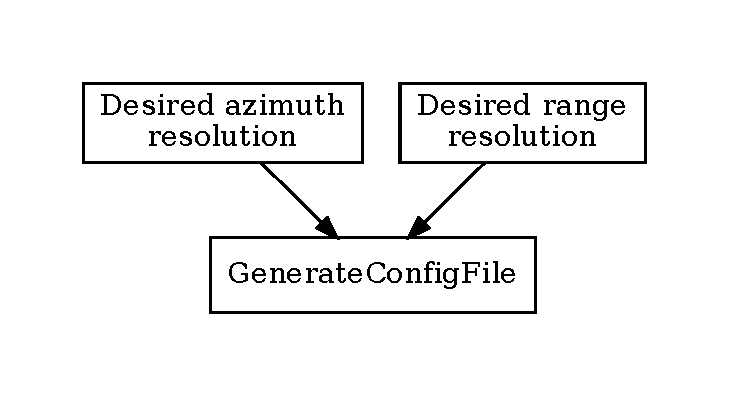
\includegraphics{sim.pdf}}
 \caption{Simulation of the SURE signal.}
 \label{fg:simflow}
 \end{center}
\end{figure}
\subsection{Generation of the raw signals}
All simulations for this paper utilize a phased array with elements of width 0.04m which are ideally spaced 0.04m apart. For instance, the phased array used for the 40cm mode is described by the XML snippet shown in listing \ref{lst:array}.
\lstset{language=XML}
\begin{lstlisting}[caption={Phased Array configuration}, label={lst:array}]
<instrument>
  <antennaArray>
    <carrierFrequency unit="Hz">9.650e9</carrierFrequency>
    <azimuthPositions unit="m">-9.980000 -9.940000 -9.900000 ...
    ... 9.900000 9.940000 9.980000</azimuthPositions>
    <azimuthElementLengths unit="m">0.040000 0.040000 0.040000 ...
    ... 0.040000 0.040000 0.040000</azimuthElementLengths>
    <transmitPowers unit="dB">10.0 10.0 10.0 ...
    ... 10.0 10.0 10.0</transmitPowers>
    <systemTemperature unit="degrees" system="Kelvin">297</systemTemperature>
    <systemLosses unit="dB">-5.3</systemLosses>
  </antennaArray>
</instrument>
\end{lstlisting}
The azimuthPositions XML field defines the position of each T/R module in the azimuth direction while the azimuthElementLength defines the width of each element.
\par
The various azimuth look directions are defined according to the angular width of each beam (which depends upon the length of the subaperture) and the span of angles required to achieve a particular azimuth resolution. In this simulation all beams are created with the same angular width. As well, the subaperture phase-centre positions are generated to be evenly spaced in the azimuth direction.
\begin{figure}[h!]
\begin{center}
 \resizebox{0.8\columnwidth}{!}{\input{subarray.pdf_tex}}
 \caption{Schematic of 5 subapertures for the 40 cm mode.}
 \label{fg:fivechansubaperture}
 \end{center}
\end{figure}
\par
As illustrated in \fgref{fg:fivechansubaperture}, the simulation generates a data array for each subaperture/beam combination. The parameters for for each subaperture/beam combination are also read from the configuration file as illustrated in listing \ref{lst:configuration}. For each of these combinations, the configuration file defines an XML element called radarConfiguration which has a channel attribute given by ``channel$m$-$n$'', where $m$ corresponds to the subaperture while $n$ corresponds to the beam. The subaperture is defined using magnitude weights for each phased-array element on both transmit and receive. The set of wieghts used on transmit may be different from those used on receive. 
\par
The beam directions are controlled by using true time-delays on both transmit and receive (although they are set to the same values in this simulation so that the transmit and receive beams are pointing in the same direction). Of course, a true time-delay approach rather than a phase-steered approach is required as we are considering a wide-band system rather than a narrow-band system.
\begin{lstlisting}[caption={Channel/Beam configuration}, label={lst:configuration}]
<radarConfiguration channel="channel0-0">
  <transmitConfiguration>
    <polarization>H</polarization>
    <u0 unit="radians">1.553329e-02</u0>
    <magnitude unit="natural">0 0 0 ... 1 1 1 ... 0 0 0</magnitude>
    <truedelay unit="ns">0.517098 0.515026 0.512953 ...</truedelay>
  </transmitConfiguration>
  <receiveConfiguration>
    <polarization>H</polarization>
    <u0 unit="radians">1.553329e-02</u0>
    <magnitude unit="natural">1 1 1 ... 0 0 0 ... 0 0 0</magnitude>
    <truedelay unit="ns">0.517098 0.515026 0.512953 ...</truedelay>
  </receiveConfiguration>
</radarConfiguration>
\end{lstlisting}
A data file for each subaperture/beam combination is created with the data stored in the undersampled azimuth-wavenumber, range-time domain. The number of samples in each of the subaperture/beam combinations is sufficient in the range direction to cover all range-cell migration and sufficient in the azimuth direction to capture all angles covered by every beam. Since the number of beams equals the number of channels, the total number of channels created is $\numberChannels = (\channelM+1)^2$.
\par
Note that in this simulation, the computed signals have no across-track baseline.
\subsection{Multichannel processing}
Multichannel processing for this simulation occurs in the azimuth-wavenumber, range-time domain. This step computes a processing filter that attempts to create a signal over an azimuth frequency range given by $\kparmPRF*(\numberChannels + 4)$; that is, when the average antenna pattern of \eqref{eq:averagePattern} is applied, there should some wavenumber domain zero-padding applied to the computed signal.
\par
Since the theory shows that the multichannel processing filter is range independent, only a single processing filter is computed an applied across all ranges. Figure \fgref{fg:reconstructed} illustrates the multichannel processing signal. In the figure, one sees that the response in the Doppler domain shows the desired response as a function of $\kparm$, with each local maximum in this region highlighting the response from each sub-beam.
\begin{figure}[ht!]
\begin{subfigure}{0.5\textwidth}
\begin{center}
 \resizebox{\columnwidth}{!}{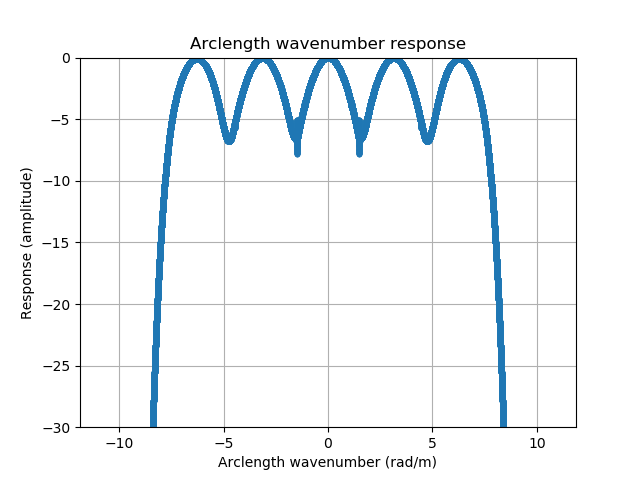
\includegraphics{simulation/40cm/simulation_plots/wk_doppler_response_amplitude.png}}
 \caption{40 cm mode.}
 \label{fg:40cmreconstructed}
 \end{center}
\end{subfigure}
\begin{subfigure}{0.5\textwidth}
\begin{center}
 \resizebox{\columnwidth}{!}{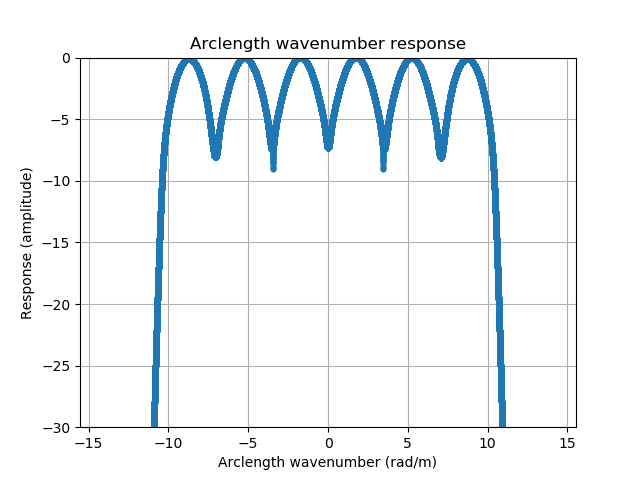
\includegraphics{simulation/30cm/simulation_plots/wk_doppler_response_amplitude.png}}
 \caption{30 cm mode.}
 \label{fg:30cmreconstructed}
 \end{center}
\end{subfigure}
\begin{subfigure}{0.5\textwidth}
\begin{center}
 \resizebox{\columnwidth}{!}{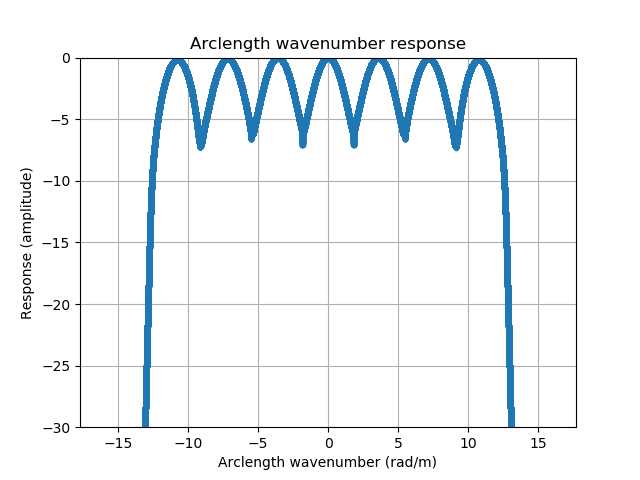
\includegraphics{simulation/25cm/simulation_plots/wk_doppler_response_amplitude.png}}
 \caption{25 cm mode.}
 \label{fg:25cmreconstructed}
 \end{center}
\end{subfigure}
\begin{subfigure}{0.5\textwidth}
\begin{center}
 \resizebox{\columnwidth}{!}{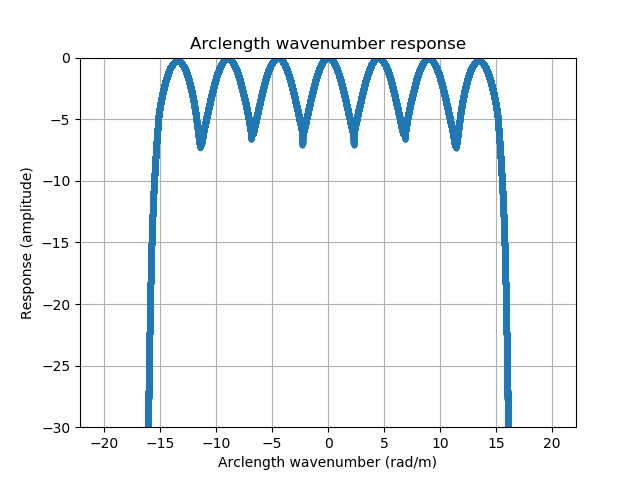
\includegraphics{simulation/20cm/simulation_plots/wk_doppler_response_amplitude.png}}
 \caption{20 cm mode.}
 \label{fg:20cmreconstructed}
 \end{center}
\end{subfigure}
\begin{subfigure}{0.5\textwidth}
\begin{center}
 \resizebox{\columnwidth}{!}{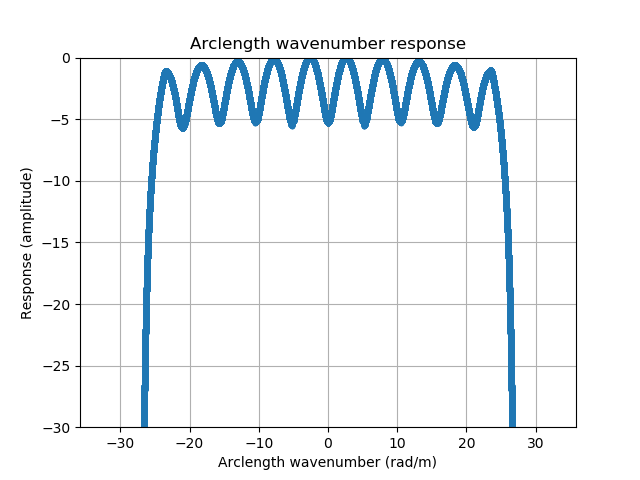
\includegraphics{simulation/12cm/simulation_plots_full/wk_doppler_response_amplitude.png}}
 \caption{12 cm mode.}
 \label{fg:12cmreconstructed}
 \end{center}
\end{subfigure}
\begin{subfigure}{0.5\textwidth}
\begin{center}
 \resizebox{\columnwidth}{!}{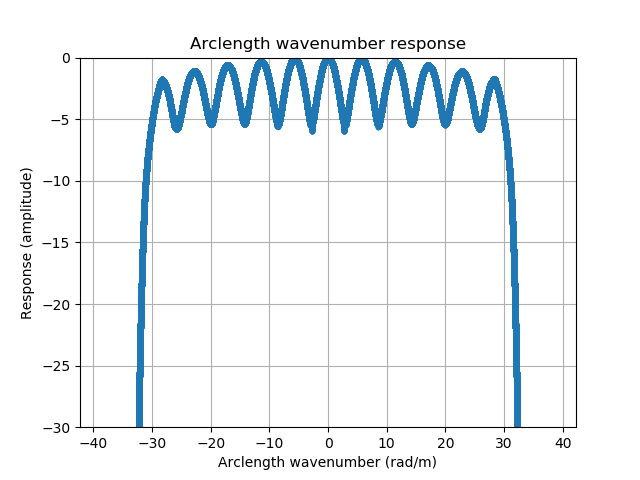
\includegraphics{simulation/10cm/simulation_plots_phase_corrected/wk_doppler_response_amplitude.png}}
 \caption{10 cm mode.}
 \label{fg:10cmreconstructed}
 \end{center}
\end{subfigure}
\caption{Reconstructed signals in azimuth wavenumber domain.}
\label{fg:reconstructed}
\end{figure}
\clearpage
\subsection{Azimuth compression}
The simulator then azimuth compresses multichannel reconstructed signal with the generalized Stolz interpolation algorithm outlined in \scref{sc:modifiedStolz}. \Fgref{fg:PSFAll} illustrates the produced the Point Spread Functions (PSF) for all modes. In these plots, the residual phase correction of \scref{sc:phaseCompensation} has not been applied.
\begin{figure}[ht!]
\begin{subfigure}{0.5\textwidth}
\begin{center}
 \resizebox{\columnwidth}{!}{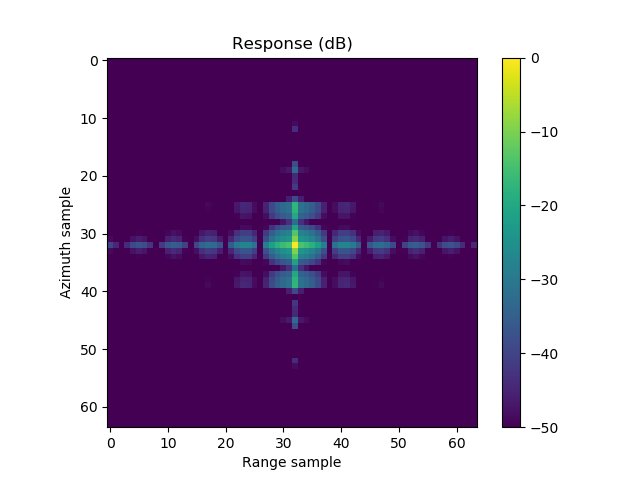
\includegraphics{simulation/40cm/simulation_plots/wk_response_32x32.png}}
 \caption{40 cm mode.}
 \label{fg:40cmPSF}
 \end{center}
\end{subfigure}
\begin{subfigure}{0.5\textwidth}
\begin{center}
 \resizebox{\columnwidth}{!}{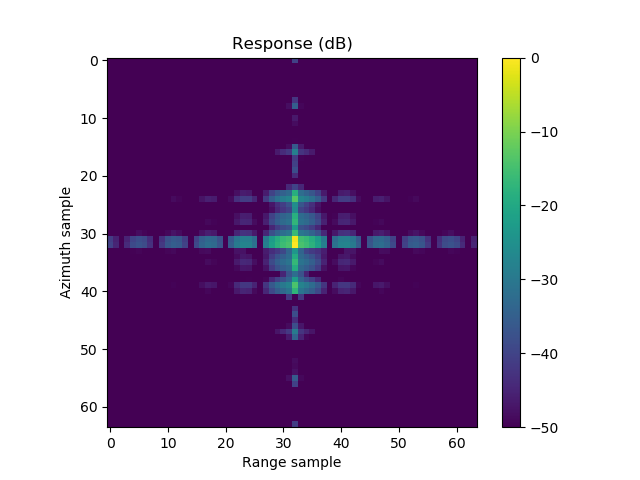
\includegraphics{simulation/30cm/simulation_plots/wk_response_32x32.png}}
 \caption{30 cm mode.}
 \label{fg:30cmPSF}
 \end{center}
\end{subfigure}
\begin{subfigure}{0.5\textwidth}
\begin{center}
 \resizebox{\columnwidth}{!}{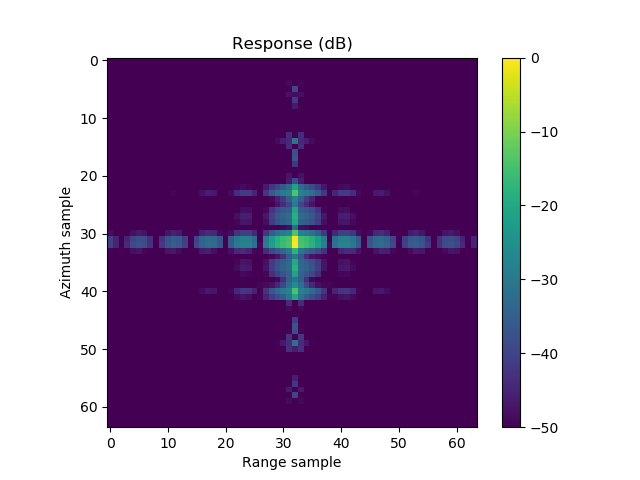
\includegraphics{simulation/25cm/simulation_plots/wk_response_32x32.png}}
 \caption{25 cm mode.}
 \label{fg:25cmPSF}
 \end{center}
\end{subfigure}
\begin{subfigure}{0.5\textwidth}
\begin{center}
 \resizebox{\columnwidth}{!}{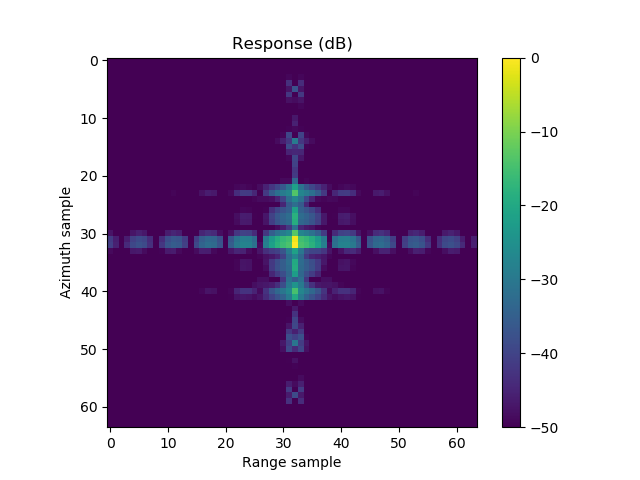
\includegraphics{simulation/20cm/simulation_plots/wk_response_32x32.png}}
 \caption{20 cm mode.}
 \label{fg:20cmPSF}
 \end{center}
\end{subfigure}
\begin{subfigure}{0.5\textwidth}
\begin{center}
 \resizebox{\columnwidth}{!}{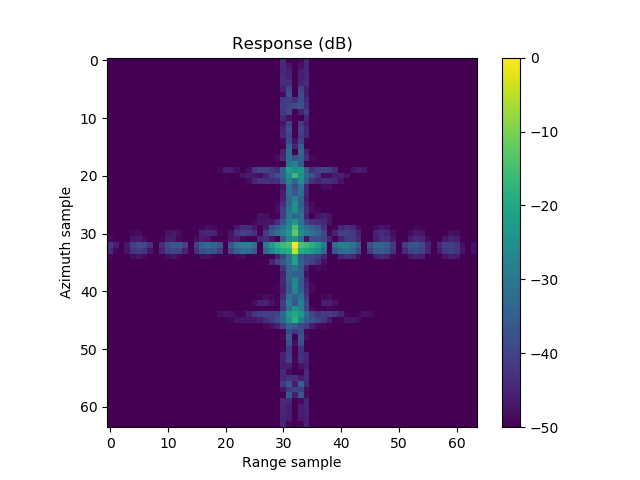
\includegraphics{simulation/12cm/simulation_plots_full/wk_response_32x32.png}}
 \caption{12 cm mode.}
 \label{fg:12cmPSF}
 \end{center}
\end{subfigure}
\begin{subfigure}{0.5\textwidth}
\begin{center}
 \resizebox{\columnwidth}{!}{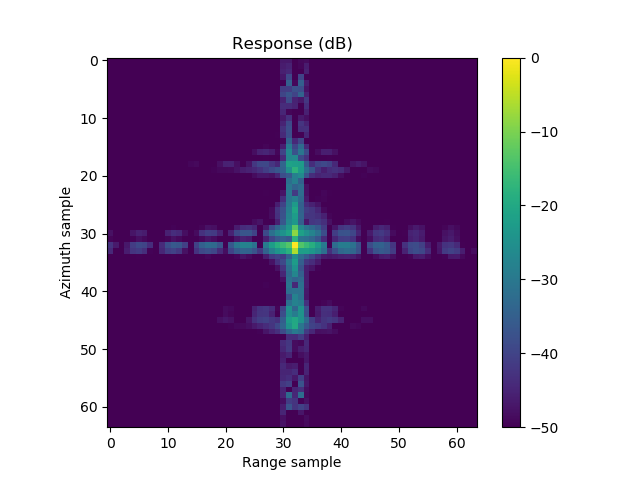
\includegraphics{simulation/10cm/simulation_plots/wk_response_32x32.png}}
 \caption{10 cm mode.}
 \label{fg:10cmPSF}
 \end{center}
\end{subfigure}
\caption{Processed signal Point Spread Response.}
\label{fg:PSFAll}
\end{figure}
\clearpage
\subsubsection{Residual phase correction}
As the resolution increases, it becomes more important to compensate for the residual phase difference that arises from the discrepancy between the differential geometry approximation to the orbit and the true satellite orbit. If examined closely, \fgref{fg:10cmPSF} shows an azimuth imbalance in the the PSF for the 10cm mode (this can also be seen in the 12cm mode and in the 20 cm mode). This imbalance is made clearer in the cross-section plot of \fgref{fg:azimuthCross10Unbalanced}
\begin{figure}[ht!]
\begin{center}
 \resizebox{\columnwidth}{!}{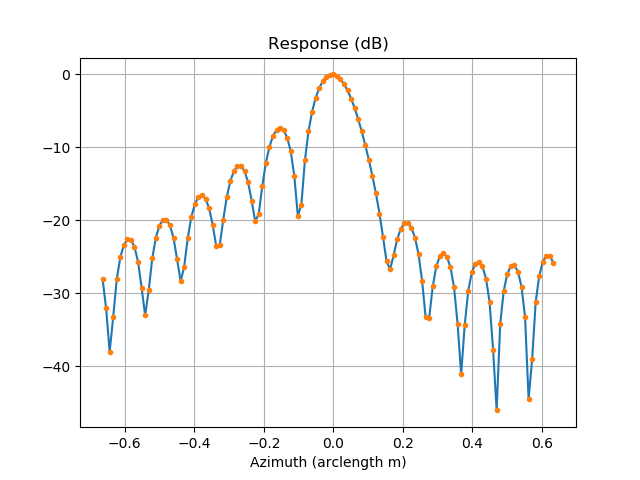
\includegraphics{simulation/10cm/simulation_plots/wk_response_s_os_8.png}}
 \caption{Azimuth cross-section of 10cm mode without residual phase correction.}
 \label{fg:azimuthCross10Unbalanced}
 \end{center}
\end{figure}
After compensating for the residual phase using the computed phase compensation described in \scref{sc:phaseCompensation}, one obtains the more desirable point spread function illustrated in \fgref{fg:10cmPSFBalanced} along with its azimuth cross-section illustrated in \fgref{fg:azimuthCross10}.
\begin{figure}[ht!]
\begin{center}
 \resizebox{\columnwidth}{!}{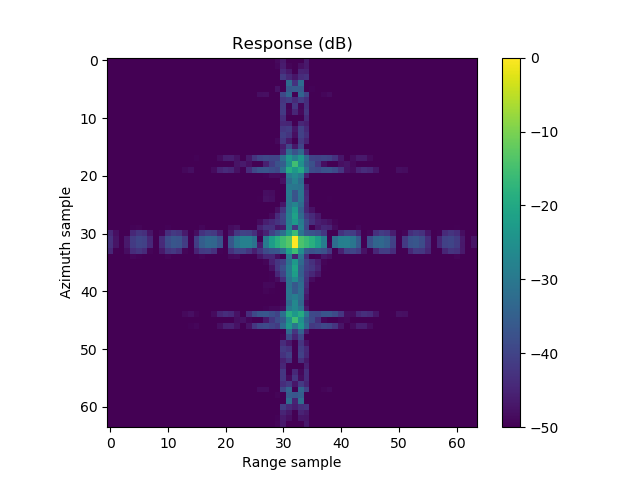
\includegraphics{simulation/10cm/simulation_plots_phase_corrected/wk_response_32x32.png}}
 \caption{Point Spread Function of 10cm mode after phase compensation.}
 \label{fg:10cmPSFBalanced}
 \end{center}
\end{figure}
\begin{figure}[ht!]
\begin{center}
 \resizebox{\columnwidth}{!}{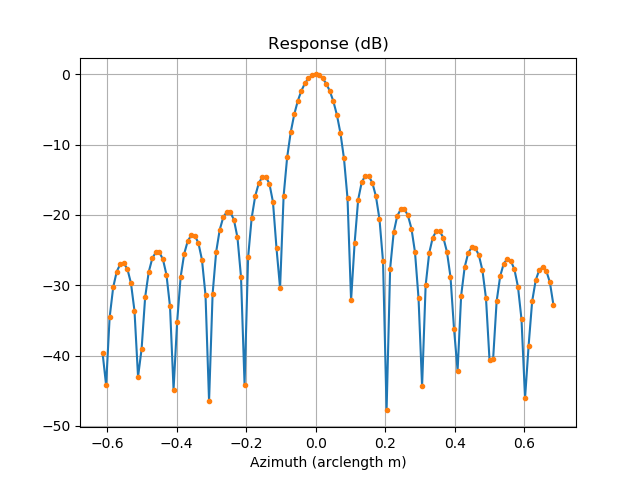
\includegraphics{simulation/10cm/simulation_plots_phase_corrected/wk_response_s_os_8.png}}
 \caption{Azimuth cross-section of 10cm mode after residual phase correction.}
 \label{fg:azimuthCross10}
 \end{center}
\end{figure}
The plot clearly illustrates a 3dB resolution of better than 10cm. Further, in the generation of sidelobes at this zoom level, the peak sidelobe level is at around -14.5dB from the peak.
\par
Over the wider range of azimuth values illustrated in \fgref{fg:azimuthCross10wide}, one observes a different generation of sidelobes. The peak of these second-level sidelobes manifests at around -18dB. A suitable weighting on the Doppler response of \fgref{fg:10cmPSF} can suppress these second-level sidelobes at the expense of resolution.
\begin{figure}[ht!]
\begin{center}
 \resizebox{\columnwidth}{!}{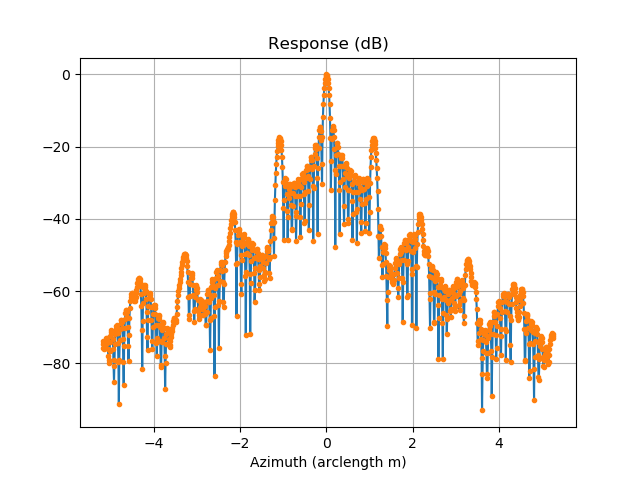
\includegraphics{simulation/10cm/simulation_plots_phase_corrected/wk_response_s_os_64.png}}
 \caption{Azimuth cross-section of 10cm mode after residual phase correction.}
 \label{fg:azimuthCross10wide}
 \end{center}
\end{figure}
% shown in \fgref{fg:psf}. This figure illustrates that the system achieves the desired resolution with the response width less than 0.1 m at the -5 dB level. While the figure also shows a second set of sidelobes at -15 dB, it is assumed that these can be reduced by an appropriate choice of weighting on the antenna patterns. 
% \begin{figure}[ht!]
% \begin{center}
%  \resizebox{\columnwidth}{!}{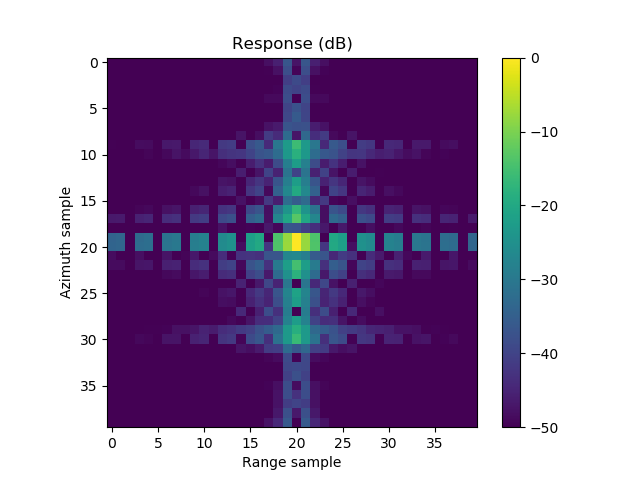
\includegraphics{simulation/Figure_11.png}}
%  \caption{Point Spread Function using the described processing method.}
%  \label{fg:psf}
%  \end{center}
% \end{figure}
% \begin{figure}[ht!]
% \begin{center}
%  \resizebox{\columnwidth}{!}{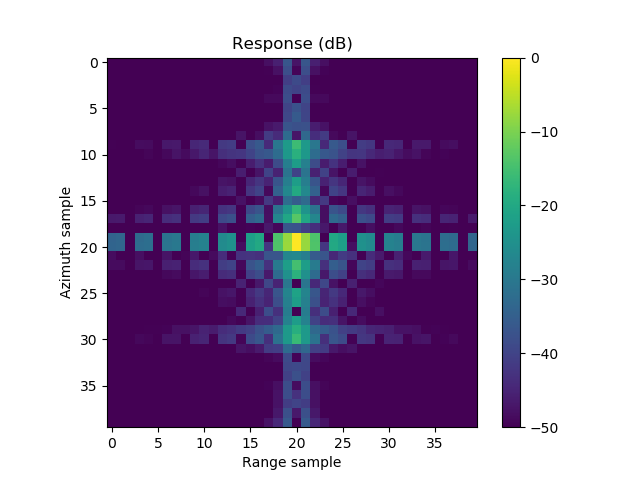
\includegraphics{simulation/Figure_11.png}}
%  \caption{Point Spread Function using the described processing method.}
%  \label{fg:psf1}
%  \end{center}
% \end{figure}
% \begin{figure}[ht!]
% \begin{center}
%  \resizebox{\columnwidth}{!}{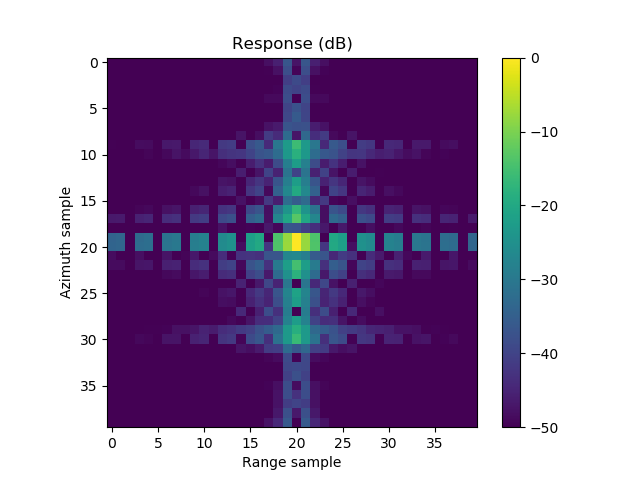
\includegraphics{simulation/Figure_11.png}}
%  \caption{Point Spread Function using the described processing method.}
%  \label{fg:psf2}
%  \end{center}
% \end{figure}
\subsubsection{Signal to noise ratio}
The PRFs selected for all simulations differ from the ``ideal'' PRF thus potentially adversely affecting the Signal to Noise Ratio (SNR). As a measure of the radiometrical resolution, the Noise Equivalent Sigma Zero (NESZ) is computed for all modes. 
Based upon parameters in the simulation configuration file, the radar equation is used to generate a estimate of the simulated signal to noise ratio. 
\par
Assuming ideal antenna elements, each with area $D_aD_e$, where $D_a$ and $D_e$ are the azimuth and elevation lengths of the antenna, then the gain of each element as a function of directional cosine $u$ in the azimuth direction and $v$ in the elevation direction may be represented as
\begin{equation}
 G_{T_x}(u,v) = G_{R_x}(u,v) = \frac{4\pi D_aD_e}{\lambda_0^2}\text{sinc}^2\left(\frac{uD_a}{\lambda_0}\right)\text{sinc}^2\left(\frac{vD_e}{\lambda_0}\right).
 \label{eq:gainPattern}
\end{equation}
This expression is such that
\begin{equation}
 \int_{-1}^1G_{T_x}(u,v)\d{u}\d{v}=4\pi,
\end{equation}
which simply means that power is preserved; however, rather than the power being evenly distributed around a sphere, it is directed, preferentially, in the direction $u=v=0$.
\par
If $P_{T_x}$ is the transmit power of each transmit element, then the true-time-delay beamforming operation (consisting of $N_{T_x}$ elements) delivers a total of power of $P_{total} = P_{T_x}N_{T_x}$, and the received SNR can be expressed as
\begin{equation}
 \frac{P_{total}G_{T_x}(u,v)A_{R_x}}{(4\pi R^2)^2Lk_BTB}\crossSection
\end{equation}
where $A_{R_x}=N_{R_x}A_e$ is the effective receive area and $A_e=D_aD_e\alpha$. Here, $\alpha<1$ accounts for the ``effective'' antenna area of each T/R module. Finally, $\crossSection$ is the backscatter cross-section. If one considers only the maximum gain (i.e. the maximum of \eqref{eq:gainPattern}), the above becomes
\begin{equation}
 \frac{P_{total}N_{R_x}A_e}{(4\pi R^2)^2Lk_BTB}\frac{4\pi N_{T_x}A_e}{\lambda_0^2}\crossSection
\end{equation}
where $A_{T_x}=N_{T_x}A_e$ is the effective area of the transmit antenna. The pulse compression gain is approximately $\tau_pB$ (where $\tau_p$ is the pulse duration), so, after pulse compression, one computes an SNR of
\begin{equation}
 \SNR_s = \frac{P_{total}N_{R_x}N_{T_x}A_e^2\tau_p}{4\pi R^4 Lk_BT\lambda_0^2}\crossSection
 \label{eq:pulseCompBeamFormedSNR}
\end{equation}
This is the SNR of each channel before multichannel and SAR processing. The simulation sets the amplitude of return signal to $\sqrt{\SNR_s}$ with $\crossSection=1$ and generates an additive zero-mean complex circular Gaussian noise signal with unit variance. This noise signal is passed though the multichannel and SAR processing steps with the same parameters used as for the signal thus simulating the processed noise. The NESZ is computed as the variance of this noise signal divided by the target signal (the maximum of the squared absolute value) yielding the results in \tbref{tb:nesz}. For all the modes simulated, the worst-case NESZ is -25 dB while the NESZ for the 10 cm mode is around -30 dB.
\begin{table}[ht!]
\begin{center}
 \caption{Computed NESZ}
 \label{tb:nesz}
 \begin{tabular}{r|l|l}
 {\bf Mode} & {\bf $f_p$} (Hz)& {\bf NESZ} (dB)\\\hline
 {\bf 40 cm} & 4500.00 & -30.9\\\hline
 {\bf 30 cm} & 5000.00 & -29.8\\\hline
 {\bf 25 cm} & 5142.86 & -29.7\\\hline
 {\bf 20 cm} & 6428.57 & -29.2\\\hline
 {\bf 12 cm} & 7500.00 & -25.5\\\hline
 {\bf 10 cm} & 8181.82 & -30.2\\\hline
 \end{tabular}
 \end{center}
\end{table}
\par
In summary, the simulation demonstrates the suitability of the proposed signal processing algorithm and also shows how the generated PSF contains extra sidelobes that most likely result from the different shape of the signal response in the Doppler domain. If these sidelobes are intolerable, they can possibly be removed by modifying the phased-array beam tables; however, this is a topic for further research. The simulation further shows that this approach to SAR imaging generates responses of very high resolution not only geometrically, but also with favourable NESZ characteristics.
\clearpage
%\section{Conclusion}
We propose a system for improved space-based SAR imaging, describing the design, which is based upon a phased-array and an appropriate switching network to allow digitisation of multiple receive channels, the configuration, which imposes a rapid electronic beam switching capability upon the design, and a suitable signal processing algorithm to compute the high resolution imagery. The proposed configuration permits measurement of a relatively large swath in a Stripmap-like mode, thereby offering, theoretically, unlimited azimuth extent. On the other hand, as demonstrated by the test example of 10cm azimuth resolution considered throughout the paper, the resolution of the imagery can be even better than the highest resolution spotlight imagery available from current commercial systems.
\par
Importantly, the state of current technology is sufficiently advanced to construct such a SAR system.
\par
As a final important consideration, we note that the design does not preclude the use of other traditional measurement modes such as Spotlight, TOPS or ScanSAR. Further, it provides the flexibility to implement other advanced modes such as HRWS and Ground Moving Target Indication.


\section{Conclusion}
We propose a system for improved space-based SAR imaging, describing the design, which is based upon a phased-array and an appropriate switching network to allow digitisation of multiple receive channels, the configuration, which imposes a rapid electronic beam switching capability upon the design, and a suitable signal processing algorithm to compute the high resolution imagery. The proposed configuration permits measurement of a relatively large swath in a Stripmap-like mode, thereby offering, theoretically, unlimited azimuth extent. On the other hand, as demonstrated by the test example of 10cm azimuth resolution considered throughout the paper, the resolution of the imagery can be even better than the highest resolution spotlight imagery available from current commercial systems.
\par
Importantly, the state of current technology is sufficiently advanced to construct such a SAR system.
\par
As a final important consideration, we note that the design does not preclude the use of other traditional measurement modes such as Spotlight, TOPS or ScanSAR. Further, it provides the flexibility to implement other advanced modes such as HRWS and Ground Moving Target Indication.


% Add the References section
\clearpage
\printbibliography
% \bibliography{refs}
% \bibliographystyle{drdc}
 
% Add some annexes
\appendix
\section{Derivative of unit vectors}
\label{an:vectorCalc}
This section provides a summary of well-known vector derivative relations. These relations can be used to tie together many of the mathematical derivations scattered throughout the document.
\par
Specifically, the section presents the derivatives of three forms of a parameterized vector with respect to the parameter. These forms include the derivative of the amplitude of the parameterized vector, the derivative of the parameterized unit vector and the derivative of the projection of a given parameterized vector in the direction perpendicular to another vector with the same parameterization.
\par
Consider
\begin{equation}
 \frac{\d{\lvert\vct{f}\rvert}}{\d{t}} = \uf^T\df
\end{equation}
from which one derives
\begin{equation}
 \frac{\d{\vct{\hat{f}}}}{\d{t}} = \frac{\d{}}{\d{t}}\frac{\vct{f}}{\lvert\vct{f}\rvert} 
 = \frac{\dot{\vct{f}} - \vct{\hat{f}}^T\dot{\vct{f}}\hat{\vct{f}}}{\lvert\vct{f}\rvert}
 = \frac{\dot{\vct{f}} - \hat{\vct{f}}\vct{\hat{f}}^T\dot{\vct{f}}}{\lvert\vct{f}\rvert}
 = \frac{\mtx{P}_\vct{f}\dot{\vct{f}}}{\lvert\vct{f}\rvert}
\end{equation}
where
\begin{equation}
 \mtx{P}_\vct{f} = \mtx{I} - \hat{\vct{f}}\vct{\hat{f}}^T
\end{equation}
where $\mtx{I}$ is the identity matrix. By inspection, one notes that pre-multiplication of a vector by the matrix $\mtx{P}_\vct{f}$ always yields the component of that vector that is perpendicular to $\vct{f}$.
\par
By using the above relations, one calculates the final relation that
\begin{equation}
 \frac{\d{}}{\d{t}}\Pf\vct{g} = -\frac{1}{\lvert\vct{f}\rvert}\left[\Pf\df\uf^T + \uf\df^T\Pf\right]\vct{g} + \Pf\dot{\vct{g}}
\end{equation}


\section{ECEF acceleration}
\label{an:inertialecef}
This section relates the equations of motion of a satellite in an Earth-Centered, Earth-Fixed (ECEF) coordinate system to those in an Earth-Centered Inertial (ECI) coordinate system. These relations play a role in propagating the orbit of a satellite since the acceleration of the satellite (derived from the egm96 gravitational potential in this document) has nothing to do with the rotation of the planet. On the other hand, SAR imaging of the ground, which rotates underneath the satellite, is most readily described in a coordinate system common both to the ground and the satellite (an ECEF system). This means that we prefer satellite position, velocity, acceleration, and the rate of change of acceleration in an ECEF coordinate system. In essence, the inertial gravitational acceleration needs to be properly interpreted in an ECEF coordinate system. We then propagate the satellite orbit in an ECEF coordinate system.
\par
Define the relation between ECEF space and inertial space as
\begin{equation}
 \vct{x}_e(t)=\mtx{M}(t)\vct{x}_i(t),
\end{equation}
and
\begin{equation}
 \vct{x}_i(t)=\mtx{M}^T(t)\vct{x}_e(t),
\end{equation}
where
\begin{equation}
 \mtx{M}(t)=\begin{bmatrix}
             \ct & -\st & 0\\
             \st & \ct  & 0\\
             0   & 0    & 1
            \end{bmatrix},
\end{equation}
where $\omega_e$ is the rotation rate of the earth.
% Note that
% \begin{equation}
%  \mtx{M}^T(t)=\begin{bmatrix}
%              \ct & \st & 0\\
%              -\st & \ct  & 0\\
%              0   & 0    & 1
%             \end{bmatrix}
% \end{equation}
Calculation of derivatives yields
\begin{equation}
 \dot{\mtx{M}}(t) = \omega_e\begin{bmatrix}
             -\st & -\ct & 0\\
             \ct & -\st  & 0\\
             0   & 0    & 0
            \end{bmatrix},
\end{equation}
\begin{equation}
 \ddot{\mtx{M}}(t) = -\omega^2_e\begin{bmatrix}
             \ct & -\st & 0\\
             \st & \ct  & 0\\
             0   & 0    & 0
            \end{bmatrix},
\end{equation}
and
\begin{equation}
 \dddot{\mtx{M}}(t) = -\omega^3_e\begin{bmatrix}
             -\st & -\ct & 0\\
             \ct & -\st  & 0\\
             0   & 0    & 0
            \end{bmatrix}.
\end{equation}
To simplfy notation, let
\begin{equation}
 \Itwo=\begin{bmatrix}
 1 & 0 & 0\\
 0 & 1 & 0\\
 0 & 0 & 0
\end{bmatrix}
\end{equation}
and
\begin{equation}
 \Qtwo=\begin{bmatrix}
 0 & -1 & 0\\
 1 & 0 & 0\\
 0 & 0 & 0
\end{bmatrix}.
\end{equation}
By direct calculation
\begin{equation}
 \Qtwo\Qtwo = -\Itwo 
\end{equation}
For use later, we compute the following
\begin{align}
\dot{\mtx{M}}(t)\mtx{M}^T(t) &= \omega_e\Qtwo\\
\ddot{\mtx{M}}(t)\mtx{M}^T(t) &= -\omega^2_e\Itwo\\
\dddot{\mtx{M}}(t)\mtx{M}^T(t) &= -\omega^3_e\Qtwo\\
\end{align}
\subsection{ECEF equations of motion}
With the previous material, one computes
\begin{align}
 \dot{\vct{x}}_e(t) &= \dot{\mtx{M}}(t)\vct{x}_i(t) + \mtx{M}(t)\dot{\vct{x}}_i(t)\\
 \ddot{\vct{x}}_e(t) &= \ddot{\mtx{M}}(t)\vct{x}_i(t) + 2\dot{\mtx{M}}(t)\dot{\vct{x}}_i(t) + \mtx{M}(t)\ddot{\vct{x}}_i(t)\\
 \dddot{\vct{x}}_e(t) &= \dddot{\mtx{M}}(t)\vct{x}_i(t) + 3\ddot{\mtx{M}}(t)\dot{\vct{x}}_i(t) + 3\dot{\mtx{M}}(t)\ddot{\vct{x}}_i(t) + \mtx{M}(t)\dddot{\vct{x}}_i(t)
\end{align}
From the first expression
\begin{equation}
\begin{split}
 \mtx{M}^T(t)\dot{\vct{x}}_e(t) &= \mtx{M}^T(t)\dot{\mtx{M}}(t)\mtx{M}^T(t)\vct{x}_e(t) + \dot{\vct{x}}_i(t)\\
 &= \omega_e\mtx{M}^T(t)\Qtwo\vct{x}_e(t) + \dot{\vct{x}}_i(t)
 \end{split}
\end{equation}
so that
\begin{equation}
 \dot{\vct{x}}_i(t) = \mtx{M}^T(t)\left[\dot{\vct{x}}_e(t) - \omega_e\Qtwo\vct{x}_e(t)\right]
\end{equation}
Substitution of this equivalence into the second expression above yields
\begin{equation}
\begin{split}
\ddot{\vct{x}}_e(t) &= \ddot{\mtx{M}}(t)\mtx{M}^T(t)\vct{x}_e(t) + 2\dot{\mtx{M}}(t)\mtx{M}^T(t)\left[\dot{\vct{x}}_e(t) - \omega_e\Qtwo\vct{x}_e(t)\right] + \mtx{M}(t)\ddot{\vct{x}}_i(t)\\
&= -\omega_e^2\Itwo\vct{x}_e(t) + 2\omega_e\Qtwo\left[\dot{\vct{x}}_e(t) - \omega_e\Qtwo\vct{x}_e(t)\right] + \mtx{M}(t)\ddot{\vct{x}}_i(t)\\
&= -\omega_e^2\Itwo\vct{x}_e(t) + 2\omega_e\Qtwo\dot{\vct{x}}_e(t) + 2\omega^2_e\Itwo\vct{x}_e(t) + \mtx{M}(t)\ddot{\vct{x}}_i(t)\\
&= \omega_e^2\Itwo\vct{x}_e(t) + 2\omega_e\Qtwo\dot{\vct{x}}_e(t) + \mtx{M}(t)\ddot{\vct{x}}_i(t)
\end{split}
\label{eq:inertialddot}
\end{equation}
and substitution into the third expression yields
\begin{equation}
\begin{split}
 \dddot{\vct{x}}_e(t) &= \dddot{\mtx{M}}(t)\mtx{M}^T(t)\vct{x}_e(t) + 3\ddot{\mtx{M}}(t)\mtx{M}^T(t)\left[\dot{\vct{x}}_e(t) - \omega_e\Qtwo\vct{x}_e(t)\right]\\
 &+ 3\dot{\mtx{M}}(t)\ddot{\vct{x}}_i(t) + \mtx{M}(t)\dddot{\vct{x}}_i(t)\\
 &= -\omega^3_e\Qtwo\vct{x}_e(t) - 3\omega_e^2\Itwo\left[\dot{\vct{x}}_e(t) - \omega_e\Qtwo\vct{x}_e(t)\right] + 3\dot{\mtx{M}}(t)\ddot{\vct{x}}_i(t) + \mtx{M}(t)\dddot{\vct{x}}_i(t)\\
 &= 2\omega^3_e\Qtwo\vct{x}_e(t) - 3\omega_e^2\Itwo\dot{\vct{x}}_e(t) + 3\dot{\mtx{M}}(t)\ddot{\vct{x}}_i(t) + \mtx{M}(t)\dddot{\vct{x}}_i(t)
 \end{split}
\label{eq:inertialdddot}
\end{equation}

\subsection{Rate of change of acceleration}
\label{an:rateacc}
This subsection computes the rate of change of acceleration of a satellite in an intertial Earth-Centered coordinate system. Further, because the egm96 gravitational potential, \eqref{eq:egm96model}, is defined using spherical-polar coordinates, this subsection also demonstrates how to convert the gradient of this potential into a Cartesian representation. The ECEF rate of change of acceleration is then given by the derivative of this acceleration with respect to time and one then acquires the ECEF equations of motion by substituting the two computed quantities into \eqref{eq:inertialddot} and \eqref{eq:inertialdddot}.
\par
The gravitational potential, $U(r,\phi,\lambda)$, is defined in \eqref{eq:egm96model}, and the gradient of this quantity defines the gravitational acceleration. We convert the gradient in spherical-polar coordinates to a graident in Cartesian coordinates, $x,y,z$, through
\begin{equation}
\begin{split}
 \ddot{\vct{x}}_i(t) &= \del_{x,y,z}U = 
 \begin{bmatrix}
  \prt{r}{x} & \prt{\phi}{x} & \prt{\lambda}{x}\\
  \prt{r}{y} & \prt{\phi}{y} & \prt{\lambda}{y}\\
  \prt{r}{z} & \prt{\phi}{z} & \prt{\lambda}{z}
 \end{bmatrix}
 \begin{bmatrix}
  \prt{U}{r}\\
  \prt{U}{\phi}\\
  \prt{U}{\lambda}
 \end{bmatrix}\\
 &= \left[\prt{(r,\phi,\lambda)}{(x,y,z)}\right]^T\del_{r,\phi,\lambda}U.
 \end{split}
\end{equation}
Note that, although the above equation does explicitely show a time dependence on the left side, the time variable has been supressed on the right to allow for more compact notation. In actual fact, the position coordinates do depend on time. More explicitely, the position of a body is given by $x(\tparm), y(\tparm), z(\tparm)$. Thus, to compute the derivative of the acceleration, one must compute
\begin{equation}
 \dddot{\vct{x}}_i(t) = \dtv{\del_{x,y,z}U}{\tparm} = 
 \begin{bmatrix}
 \prttwoa{U}{x} & \prttwob{U}{y}{x} & \prttwob{U}{z}{x}\\
 \prttwob{U}{x}{y} & \prttwoa{U}{y} & \prttwob{U}{z}{y}\\
 \prttwob{U}{x}{z} & \prttwob{U}{y}{z} & \prttwoa{U}{z}
 \end{bmatrix}
 \begin{bmatrix}
 \dtv{x}{\tparm} \\ \dtv{y}{\tparm} \\ \dtv{z}{\tparm}  
 \end{bmatrix}
\end{equation}
A representative component of the matrix in the above may be written as
\begin{equation}
\begin{split}
 \prttwob{U}{x_i}{x_j} &= \prt{\prt{U}{x_j}}{x_i}\\
 &=\prt{}{x_i}
 \begin{bmatrix}
  \prt{r}{x_j} & \prt{\phi}{x_j} & \prt{\lambda}{x_j}
 \end{bmatrix}
 \begin{bmatrix}
  \prt{U}{r}\\
  \prt{U}{\phi}\\
  \prt{U}{\lambda}
 \end{bmatrix}\\
 &=\begin{bmatrix}
  \prttwob{r}{x_i}{x_j} & \prttwob{\phi}{x_i}{x_j} & \prttwob{\lambda}{x_i}{x_j}
 \end{bmatrix}
 \begin{bmatrix}
  \prt{U}{r}\\
  \prt{U}{\phi}\\
  \prt{U}{\lambda}
 \end{bmatrix} +
 \begin{bmatrix}
  \prt{r}{x_j} & \prt{\phi}{x_j} & \prt{\lambda}{x_j}
 \end{bmatrix}
 \begin{bmatrix}
  \prttwob{U}{x_i}{r}\\
  \prttwob{U}{x_i}{\phi}\\
  \prttwob{U}{x_i}{\lambda}
 \end{bmatrix}\\
 &=
 \begin{bmatrix}
  \prt{U}{r} & \prt{U}{\phi} & \prt{U}{\lambda}
 \end{bmatrix}\begin{bmatrix}
  \prttwob{r}{x_i}{x_j} \\ \prttwob{\phi}{x_i}{x_j} \\ \prttwob{\lambda}{x_i}{x_j}
 \end{bmatrix} +
 \begin{bmatrix}
  \prt{r}{x_j} & \prt{\phi}{x_j} & \prt{\lambda}{x_j}
 \end{bmatrix}
 \begin{bmatrix}
  \prttwoa{U}{r} & \prttwob{U}{\phi}{r} & \prttwob{U}{\lambda}{r}\\
  \prttwob{U}{r}{\phi} & \prttwoa{U}{\phi} & \prttwob{U}{\lambda}{\phi}\\
  \prttwob{U}{r}{\lambda} & \prttwob{U}{\phi}{\lambda} & \prttwoa{U}{\lambda}
 \end{bmatrix}
 \begin{bmatrix}
  \prt{r}{x_i} \\ \prt{\phi}{x_i} \\ \prt{\lambda}{x_i}
 \end{bmatrix}
 \end{split}
\end{equation}
One can consolidate all the terms into matrix form via
\begin{equation}
\begin{split}
 &\dddot{\vct{x}}_i(t) = \dtv{\del_{x,y,z}U}{\tparm} = \\
 &\begin{bmatrix}
  \prt{U}{r} & \prt{U}{\phi} & \prt{U}{\lambda} & 0 & 0 & 0 & 0 & 0 & 0\\
  0 & 0 & 0 & \prt{U}{r} & \prt{U}{\phi} & \prt{U}{\lambda} & 0 & 0 & 0\\
  0 & 0 & 0 & 0 & 0 & 0 & \prt{U}{r} & \prt{U}{\phi} & \prt{U}{\lambda} 
 \end{bmatrix}\begin{bmatrix}
  \prttwob{r}{x}{x} & \prttwob{r}{x}{y} & \prttwob{r}{x}{z}\\ 
  \prttwob{\phi}{x}{x} & \prttwob{\phi}{x}{y} & \prttwob{\phi}{x}{z}\\ 
  \prttwob{\lambda}{x}{x} & \prttwob{\lambda}{x}{y} & \prttwob{\lambda}{x}{z}\\
  \prttwob{r}{y}{x} & \prttwob{r}{y}{y} & \prttwob{r}{y}{z}\\ 
  \prttwob{\phi}{y}{x} & \prttwob{\phi}{y}{y} & \prttwob{\phi}{y}{z}\\ 
  \prttwob{\lambda}{y}{x} & \prttwob{\lambda}{y}{y} & \prttwob{\lambda}{y}{z}\\
  \prttwob{r}{z}{x} & \prttwob{r}{z}{y} & \prttwob{r}{z}{z}\\ 
  \prttwob{\phi}{z}{x} & \prttwob{\phi}{z}{y} & \prttwob{\phi}{z}{z}\\ 
  \prttwob{\lambda}{z}{x} & \prttwob{\lambda}{z}{y} & \prttwob{\lambda}{z}{z}
 \end{bmatrix}
 \begin{bmatrix}
  \dtv{x}{\tparm} \\ \dtv{y}{\tparm} \\ \dtv{z}{\tparm}  
 \end{bmatrix}\\
 +
 &\begin{bmatrix}
  \prt{r}{x} & \prt{\phi}{x} & \prt{\lambda}{x}\\
  \prt{r}{y} & \prt{\phi}{y} & \prt{\lambda}{y}\\
  \prt{r}{z} & \prt{\phi}{z} & \prt{\lambda}{z}
 \end{bmatrix}
 \begin{bmatrix}
  \prttwoa{U}{r} & \prttwob{U}{\phi}{r} & \prttwob{U}{\lambda}{r}\\
  \prttwob{U}{r}{\phi} & \prttwoa{U}{\phi} & \prttwob{U}{\lambda}{\phi}\\
  \prttwob{U}{r}{\lambda} & \prttwob{U}{\phi}{\lambda} & \prttwoa{U}{\lambda}
 \end{bmatrix}
 \begin{bmatrix}
  \prt{r}{x} & \prt{r}{y} & \prt{r}{z}\\ 
  \prt{\phi}{x} & \prt{\phi}{y} & \prt{\phi}{z}\\ 
  \prt{\lambda}{x} & \prt{\lambda}{y} & \prt{\lambda}{z}
 \end{bmatrix}
 \begin{bmatrix}
  \dtv{x}{\tparm} \\ \dtv{y}{\tparm} \\ \dtv{z}{\tparm}  
 \end{bmatrix}
 \end{split}
\end{equation}

\section{Derivation of the arclength-parameterized range function}
\label{an:rangeComputation}
The range between the satellite and a target plays a critical role in SAR processing. This section presents an arclength parameterized expression for this range function. The final approximation of the section, \eqref{eq:rangeInvariant}, yields a version of the function that only weakly depends on the expansion point used to describe the satellite orbit.
\par
For every scatterer at point $\vct\target$, there is an arclength value, $\targetxparm$, such that $\satp(\targetxparm) - \vct\target$ is perpendicular to $\satp'(\targetxparm)$. Further, $\vct\target$ can be completely determined by 
\begin{equation}
 \vct\target = \satp(\targetxparm) + \targetrange\cos\targetdepression\vct{N}(\targetxparm) + \targetrange\sin\targetdepression\vct{B}(\targetxparm),
\end{equation}
where $\targetrange=\lvert\satp(\targetxparm)-\vct\target\rvert$ and $\targetrange\cos\targetdepression = [\vct\target - \satp(\targetxparm)]\cdot\vct{N}(\targetxparm)$.
\par
One computes that
\begin{equation}
\begin{split}
 \satp(\parm)-\vct\target &= \satp(\parm) - \satp(\targetxparm) - \targetrange\cos\targetdepression\vct{N}(\targetxparm) - \targetrange\sin\targetdepression\vct{B}(\targetxparm)\\
 &= (\parm-\targetxparm)\vct{T}_0 + \frac{(\parm-\parm_0)^2 - (\targetxparm - \parm_0)^2}{2}\kappa_0\vct{N}_0\\
 &+\frac{(\parm-\parm_0)^3 - (\targetxparm - \parm_0)^3}{6}[-\kappa^2_0\vct{T}_0 + {\kappa'}_0\vct{N}_0 + \kappa_0\tau_0\vct{B}_0]\\
 &- \targetrange\cos\targetdepression\vct{N}(\targetxparm) - \targetrange\sin\targetdepression\vct{B}(\targetxparm)\\
 &= (a-b)\biggl[\vct{T}_0 + \frac{a+b}{2}\kappa_0\vct{N}_0 +\frac{a^2+ab+b^2}{6}[-\kappa^2_0\vct{T}_0 + {\kappa'}_0\vct{N}_0 + \kappa_0\tau_0\vct{B}_0]\biggr]\\
 &- \targetrange\cos\targetdepression\vct{N}(\targetxparm) - \targetrange\sin\targetdepression\vct{B}(\targetxparm)
 \end{split},
\end{equation}
where
\begin{align}
 a &= (\parm-\parm_0)\\
 b &= (\targetxparm - \parm_0)
\end{align}
More succinctly, one can write
\begin{equation}
 \satp(\parm)-\vct\target = (a-b)(\alpha_T\vct{T}_0 + \alpha_N\vct{N}_0 + \alpha_B\vct{B}_0)- \targetrange\cos\targetdepression\vct{N}(\targetxparm) - \targetrange\sin\targetdepression\vct{B}(\targetxparm)
\end{equation}
where
\begin{align}
 \alpha_T &= 1 - \kappa^2_0\frac{a^2+ab+b^2}{6}\\
 \alpha_N &= \kappa_0\frac{a+b}{2} + {\kappa'}_0\frac{a^2+ab+b^2}{6}\\
 \alpha_B &= \kappa_0\tau_0\frac{a^2+ab+b^2}{6}
\end{align}
From the Frenet-Serret equations, \eqref{eq:FrenetSerret}, one can make the approximation that
\begin{align}
 \targetrange\cos\targetdepression\vct{N}(\targetxparm)&\approx\targetrange\cos\targetdepression\vct{N}_0 + (\targetxparm-\parm_0)\targetrange\cos\targetdepression(-\kappa_0\vct{T}_0 + \tau_0\vct{B}_0)\\
 \targetrange\sin\targetdepression\vct{B}(\targetxparm)&\approx\targetrange\sin\targetdepression\vct{B}_0 - (\targetxparm-\parm_0)\targetrange\sin\targetdepression\tau_0\vct{N}_0
\end{align}
and since $\targetxparm-\parm_0 = b$, the range expression can be written as
\begin{equation}
\begin{split}
 \satp(\parm)-\vct\target &= [(a-b)\alpha_T + b\targetrange\kappa_0\cos\targetdepression]\vct{T}_0\\
 &+ [(a-b)\alpha_N - \targetrange\cos\targetdepression + b\targetrange\tau_0\sin\targetdepression]\vct{N}_0\\
 &+ [(a-b)\alpha_B- \targetrange\sin\targetdepression - b\targetrange\tau_0\cos\targetdepression]\vct{B}_0
 \end{split}
\end{equation}
The computation of square of the above expression yields a polynomial in $(a-b) = (\parm-\targetxparm)$ (after using sagemath),
\begin{equation}
 \lvert\satp(\parm)-\vct\target\rvert^2 = \sum_{k=0}^5\rcoeff_k(\parm-\targetxparm)^k
\end{equation}
with the following coefficients
\begin{equation}
 \begin{split}
 \rcoeff_0 &= b^{2}\kappa_0^2\targetrange^2\cos^2\targetdepression + b^2\targetrange^{2}\tau_0^{2} + \targetrange^{2}\\
 \rcoeff_1 &= \frac{2b^2\tau_0\targetrange}{3}(b{\kappa'}_0 + 2\kappa_0)\sin\targetdepression - \frac{2b^2\targetrange}{3}(b\kappa_0\tau_0^2 + b\kappa_0^3 + {\kappa'}_0)\cos\targetdepression\\
 \rcoeff_2 &= 1 - [\kappa_0+b{\kappa'}_0 + b^2(\kappa_0^3 + \kappa_0\tau_0^2)]\targetrange\cos\targetdepression + b^2{\kappa'}_0\tau_0\targetrange\sin\targetdepression\\ 
 &+ \frac{b^4}{9}(\kappa_0^4+\kappa_0^2\tau_0^2 + {\kappa'}_0^2) + \frac{b^2\kappa_0}{3}(\kappa_0 + 2b{\kappa'}_0)\\
 \rcoeff_3 &= -\frac{\targetrange}{3}(\kappa_0\tau_0\sin\targetdepression + {\kappa'}_0\cos\targetdepression) + \frac{b^3}{3}(\kappa_0^4+\kappa_0^2\tau_0^2 + {\kappa'}_0^2) + \frac{4b^2}{3}\kappa_0{\kappa'}_0\\ 
 &+ \frac{b\targetrange}{3}[{\kappa'}_0\tau_0\sin\targetdepression - (\kappa_0\tau_0^2+\kappa_0^3)\cos\targetdepression]\\
 \rcoeff_4 &= -\frac{\kappa_0^2}{12} + \frac{13b^2}{36}(\kappa_0^4+\kappa_0^2\tau_0^2 + {\kappa'}_0^2) + \frac{5b\kappa_0{\kappa'}_0}{6}\\
 \rcoeff_5 &= \frac{b}{6}(\kappa_0^4+\kappa_0^2\tau_0^2 + {\kappa'}_0^2 + \kappa{\kappa'}_0)\\
 \rcoeff_6 &= \frac{1}{36}(\kappa_0^4+\kappa_0^2\tau_0^2 + {\kappa'}_0^2)
 \end{split}
 \label{eq:rangeVariant}
\end{equation}
In the region of the chosen point of expansion, $\parm_0$, $b$ evaluates to a relatively small number, thus, one can make the approximation that
\begin{equation}
 \begin{split}
 \rcoeff_0 &= \targetrange^{2}\\
 \rcoeff_1 &= 0\\
 \rcoeff_2 &= 1 - \kappa_0\targetrange\cos\targetdepression\\
 \rcoeff_3 &= -\frac{\targetrange}{3}(\kappa_0\tau_0\sin\targetdepression + {\kappa'}_0\cos\targetdepression)\\
 \rcoeff_4 &= -\frac{\kappa_0^2}{12}\\
 \rcoeff_5 &= 0\\
 \rcoeff_6 &= 0
 \end{split}
 \label{eq:rangeInvariant}
\end{equation}

\section{Iteration to the stationary point}
\label{sc:stationaryIteration}
This section illustrates convergence of the procedure of \eqref{eq:Sdefinition}. Recall that the requirement is to compute $\parm$ from
\begin{equation}
 \xang = \parm\gfunc(\parm),
\end{equation}
and to invert the above, we suggested that
\begin{equation}
\begin{split}
 \parm &= \frac{\xang}{\gfunc(\parm)} = \frac{\xang}{\gfunc\left(\frac{\xang}{\gfunc(\parm)}\right)} = \frac{\xang}{\gfunc\left(\frac{\xang}{\gfunc\left(\frac{\xang}{\gfunc(\parm)}\right)}\right)} = ...\\
 \gfunc(\parm) &= \gfunc\left(\frac{\xang}{\gfunc(\parm)}\right) = \gfunc\left(\frac{\xang}{\gfunc\left(\frac{\xang}{\gfunc(\parm)}\right)}\right) = ...
\end{split}
\end{equation}
Re-write the expression to invert as
\begin{equation}
 \frac{\xang}{\gfunc(\parm)} - \parm = 0
\end{equation}
and define the two functions
\begin{align}
 f_1(\parm) &= \parm,\\
 f_2(\parm) &= \frac{\xang}{\gfunc(\parm)}.
\end{align}
The task is then to compute the point where these two functions intersect.
\begin{figure}[ht!]
    \begin{center}
    \resizebox{0.5\textwidth}{!}{\input{iteration.pdf_tex}}
	\caption{Simple iterative procedure showing convergence to the stationary point}
	\label{fg:stationaryiteration}
	\end{center}
\end{figure}
From \fgref{fg:stationaryiteration}, one sees that, starting from the point $\parm_0$
\begin{equation}
 \parm_1 = f_2(\parm_0) = \frac{\xang}{\gfunc(\parm_0)},
\end{equation}
and, in general
\begin{equation}
 \parm_{n+1} = f_2(\parm_n) = \frac{\xang}{\gfunc(\parm_n)}.
\end{equation}
If 
\begin{equation} 
    \left\lvert \dtv{f_2(\parm)}{\parm}\right\rvert < 1,
\end{equation}
then convergence is assured.

\section{Numerical implementation of the Stolz interpolation}
\label{an:stolz}
This section outlines an approach to support numerical implementation of the proposed, generalized Stolz interpolation. Because the generalized Stolz interpolation points do not have a closed form as they do in, for instance, \cite{Cumming2005, Bamler1992}, this section presents a numerical approach. There is nothing particularly insightful about the proposed algorithm; in fact, this section aims to present an approach that avoids confusion and facilitates numerical implementation.
\par
So, to begin, recall that
\begin{equation}
 \xang = -\targetrange\tan\thetas,
\end{equation}
so that
\begin{align}
 \sin\thetas &= -\frac{\xang}{\sqrt{\targetrange^2+\xang^2}}\label{eq:angsin}\\
 \cos\thetas &= \frac{\targetrange}{\sqrt{\targetrange^2+\xang^2}}\label{eq:angcos}.
\end{align}
Alos recall that
\begin{equation}
 -\frac{\xang}{\sqrt{\targetrange^2+\xang^2}}\biggl[\gfunc(\parm)+\frac{\rcoeff_3\xang}{2\gfunc^2(\parm)}+\frac{\rcoeff_4\xang^2}{\gfunc^3(\parm)}\biggr] = \frac{\kparm}{\kr}.
\end{equation}
From \eqref{eq:newStolz}, when one makes the (Stolt interpolation) change of variables,
\begin{equation}
 \krstolt = \kr\sec\thetas - \kparm\frac{\tan\thetas}{\gfunc(\parm)},
\end{equation}
which leads to the relation that
\begin{equation}
 \kr = \frac{\targetrange\krstolt}{\sqrt{\targetrange^2+\xang^2}} - \frac{\kparm\xang}{\gfunc(\parm)\sqrt{\targetrange^2+\xang^2}}.
\end{equation}
\subsection{Simplification for iterative root-finding}
In the opinion of the authors, implementation of the Stolz interpolation (into computer code) benefits from defining the following function
\begin{equation}
 \shelp{l}{m}{n} = \frac{\xang^l}{(\targetrange^2+\xang^2)^m\gfunc^n(\parm)}
\end{equation}
The Newton iterative root finding method requires computation of the derivative of the above function, which, in turn, requires caculation of the derivative of $\gfunc(\parm)$ with respect to $\xang$. Specifically,
\begin{equation}
\begin{split}
 \frac{\d\gfunc(\parm)}{\d\xang} &= \frac{\d\gfunc(\parm)}{\d\parm}\frac{\d\parm}{\d\xang}\\
 &=\frac{\rcoeff_3+2\rcoeff_4\parm}{2\gfunc(\parm)}\frac{\d\parm}{\d\xang}\\
 &=\left(\frac{\rcoeff_3}{2\gfunc(\parm)}+\frac{\rcoeff_4\xang}{\gfunc^2(\parm)}\right)\frac{\d\parm}{\d\xang}
\end{split}
\label{eq:dgpart1}
\end{equation}
Because $\xang=\parm\gfunc(\parm)$, one derives
\begin{equation}
\begin{split}
 1 &= \frac{\d\parm}{\d\xang}\gfunc(\xparm) + \parm\frac{\d\gfunc(\parm)}{\d\parm}\frac{\d\parm}{\d\xang}\\
 & = \frac{\d\parm}{\d\xang}\left[\gfunc(\xparm) + \parm\frac{\rcoeff_3+2\rcoeff_4\parm}{2\gfunc(\parm)}\right]\\
 & = \frac{\d\parm}{\d\xang}\left[\gfunc(\xparm) + \frac{\xang}{\gfunc(\parm)}\left(\frac{\rcoeff_3}{2\gfunc(\parm)} + \frac{\rcoeff_4\xang}{\gfunc^2(\parm)}\right)\right]\\
\end{split}
\label{eq:dgpart2}
\end{equation}
By substituting \eqref{eq:dgpart2} into \eqref{eq:dgpart1}, one arrives at
\begin{equation}
 \frac{\d\gfunc(\parm)}{\d\xang} = \frac{\rcoeff_3\gfunc^2(\xparm) + 2\rcoeff_4\xang\gfunc(\xparm)}{2\gfunc^4(\xparm) + \rcoeff_3\xang\gfunc(\xparm) + 2\rcoeff_4\xang^2}
\end{equation}
The derivative of $\shelp{l}{m}{n}$ is thus given by\footnote{For use in a Newton numerical, iterative, root-finding procedure},
\begin{multline}
 \frac{\d\shelp{l}{m}{n}}{\d\xang} = \shelp{l-1}{m}{n}\\
 \left(l-m\frac{2\xang^2}{\targetrange^2+\xang^2} - n\frac{\rcoeff_3\xang\gfunc(\xparm) + 2\rcoeff_4\xang^2}{2\gfunc^4(\xparm) + \rcoeff_3\xang\gfunc(\xparm) + 2\rcoeff_4\xang^2}\right)
\end{multline}
\par
With the aforementioned definition,
\begin{equation}
 \kr = \targetrange\krstolt\shelp{0}{1/2}{0} - \kparm\shelp{1}{1/2}{1},
 \label{eq:stoltRelation}
\end{equation}
and, when this is substituted into \eqref{eq:angleRelation}, along with the realtions in \eqref{eq:angsin} and \eqref{eq:angcos}, one obtains
\begin{equation}
\begin{split}
 &\targetrange\krstolt\shelp{1}{1}{-1} - \kparm\shelp{2}{1}{0}
 +\frac{\targetrange\krstolt\rcoeff_3}{2}\shelp{2}{1}{2}\\
 &+\left(\targetrange\krstolt\rcoeff_4-\frac{\rcoeff_3\kparm}{2}\right)\shelp{3}{1}{3}
 - \rcoeff_4\kparm\shelp{4}{1}{4} + \kparm = 0
\end{split}
\label{eq:stoltInversionX}
\end{equation}
Equation \ref{eq:stoltInversionX} permits numerical computation of $\xang$ given values for $\kparm$ and $\krstolt$. This computed value for $\xang$ can be inserted into \ref{eq:stoltRelation} to provide the particular value of $\kr$ at which the data need to be estimated (through interpolation).

\section{MIMO configuration}
\label{an:mimo}
This section demonstrates how subarrays of a uniform phased array antenna can be combined to yield signals of the form of \eqref{eq:antennaArgument2}. In the configuration described below, Transmit/Receive T/R modules form the basic element of the phased array. 
\par
As illustrated in \fgref{fg:mimo}, 
\begin{figure}[ht!]
    \resizebox{\textwidth}{!}{\input{mimoconfig.pdf_tex}}
	\caption{Configuration of transmit and receive. Each transmitted signal is received by all receivers}
	\label{fg:mimo}
\end{figure}
assume that every transmission, from every element, is received and summed independently (i.e. assume superposition applies). Assume further that signals are transmitted at time $\fasttime$, but with different delays on transmission (programmed delays) for each T/R module
and that the echoes of these signals are received at time $\fasttime + 2\targetrange(\parm)/c$, but with different Rx delays for each T/R module (programmed delays)
\par
Now, the time delay to irradiate a target depends on the position of the transmitter and the location of the target. In the model, we denote the target position as $\targetxparm$ and the position of each transmitter and receiver as $\anTx{\txn}$, $\txn\in\{0, \txN-1\}$ and $\anRx{\txm}$, $\txm\in\{0, \txM-1\}$, respectively. We also denote the transmitted waveform as 
\begin{equation}
 \pulse(\fasttime)=\envelope(\fasttime)\eex{\im\omega_0\fasttime},
\end{equation}
where $\envelope(\fasttime)$ is some baseband waveform. With this notation, and with transmit and receive delays given by $\txDelay{\txn}$ and $\rxDelay{\txm}$, respectively, the far field delay for a transmit/receive pair is given by
\begin{equation}  \mnDelay(\parm) = \frac{2\amplitude\range(\parm, \targetnoparm)}{c} + \txDelay{\txn} + \rxDelay{\txn} 
+ \frac{\anTx{\txn}\cdot\uRangeVectorParm}{c} + \frac{\anRx{\txm}\cdot\uRangeVectorParm}{c}
\end{equation}
and the return signal is given by 
\begin{equation}
\pulse_{mn}(\fasttime, \parm) = \txAmp{\txn}\rxAmp{\txm}\pulse[\fasttime - \mnDelay(\parm)],
\end{equation}
where $\txAmp{\txn}$ and $\rxAmp{\txm}$ denote the antenna gains for transmit and receive from channels $\txn,\txm$, respectively.
Through the principle of superposition, the system measured signal is given by
\begin{equation}
\begin{split}
\pulse_{s}(\fasttime, \parm) &= \sum_{\txm,\txn}\pulse_{\txm\txn}(\fasttime, \parm)\\
&=\sum_{\txm,\txn}\txAmp{\txn}\rxAmp{\txm}\pulse[\fasttime - \mnDelay(\parm)].
\end{split}
\end{equation}
In the fast-time frequency domain, this signal can be written as
\begin{equation}
\begin{split}
\Pulse_{s}(\omega', \parm)&=\sum_{\txm,\txn}\txAmp{\txn}\rxAmp{\txm}\Pulse(\omega')\eex{-\im\omega'\mnDelay(\parm)}\\
&=\Pulse(\omega')\eex{-\im\omega'\frac{2\amplitude\range(\parm, \targetnoparm)}{c}}\sum_{\txn}\txAmp{\txn}\eex{-\im\omega'[\txDelay{\txn}+\frac{\anTx{\txn}\cdot\uRangeVectorParm}{c}]}\\
&\cdot\sum_{\txm}\rxAmp{\txm}\eex{-\im\omega'[\rxDelay{\txm}+\frac{\anRx{\txm}\cdot\uRangeVectorParm}{c}]},
\end{split}
\end{equation}
where $\omega'=\omega+\omega_0$.
\par
Suppose that $\anTx{\txn} = \txn\bline$ and that $\anRx{\txm} = \txm\bline$, i.e. a uniformly spaced array, and that the timing delays are chosen such that $\txDelay{\txn} = -\txn\bline\cdot\uzero/c$ and $\rxDelay{\txm} = -\txm\bline\cdot\uzero/c$ for some given look vector $\uzero$. In this case, the signal becomes
 \begin{equation}
 \begin{split}
  \Pulse_{s}(\omega', \parm)&=\Pulse(\omega')\eex{-\im\omega'\frac{2\amplitude\range(\parm, \targetnoparm)}{c}}\sum_{\txn}\txAmp{\txn}\eex{-\im\omega'\frac{\txn}{c}\bline\cdot[-\uzero+\uRangeVectorParm]}\\
  &\cdot\sum_{\txm}\rxAmp{\txm}\eex{-\im\omega'\frac{\txm}{c}\bline\cdot[-\uzero+\uRangeVectorParm]}
 \end{split}
 \end{equation}
Further, suppose that the weights, $\txAmp{\txn}$ and $\rxAmp{\txm}$, are such that $\exists \txn_\channelIndex, \txm_\channelIndex$ with the properties that both
 \begin{equation}
  \sum_{\txn}\txAmp{\txn}\eex{-\im\omega'\frac{\txn-\txn_\channelIndex}{c}\bline\cdot[-\uzero+\uRangeVectorParm]}
 \end{equation}
 and
 \begin{equation}
  \sum_{\txm}\rxAmp{\txm}\eex{-\im\omega'\frac{\txm-\txm_\channelIndex}{c}\bline\cdot[-\uzero+\uRangeVectorParm]}
 \end{equation}
 are real $\forall\omega'$. As a particular example, if $\txAmp{\txn}=A_{T_x}$, a constant, for $\txn\in\{\txn_0, \txn_0+1, \txn_0+2, \ldots, \txn_0+\txN-1\}$, then $\txn_\channelIndex=\txn_0+\txN/2$. With this condition,
 \begin{equation}
 \begin{split}
  \Pulse_{s}(\omega', \parm)&=\Pulse(\omega')\eex{-\im\omega'\frac{2\amplitude\range(\parm, \targetnoparm)}{c}}\eex{-\im\omega'\frac{\txn_\channelIndex}{c}\bline\cdot[-\uzero+\uRangeVectorParm]}\eex{-\im\omega'\frac{\txm_\channelIndex}{c}\bline\cdot[-\uzero+\uRangeVectorParm]}\\&\sum_{\txn}\txAmp{\txn}\eex{-\im\omega'\frac{\txn-\txn_\channelIndex}{c}\bline\cdot[-\uzero+\uRangeVectorParm]}
  \sum_{\txm}\rxAmp{\txm}\eex{-\im\omega'\frac{\txm-\txm_\channelIndex}{c}\bline\cdot[-\uzero+\uRangeVectorParm]}
 \end{split}
 \end{equation}
With $\omega'/c=\kr/2$, let
 \begin{equation}
  \pAntennaParm{\channelIndex} = \frac{\txn_\channelIndex\bline + \txm_\channelIndex\bline}{2},
 \end{equation}
 and define
 \begin{equation}
 \begin{split}
  \dPattern{\channelIndex}[\kr, \uRangeVectorParm] = 
  &\sum_{\txn}\txAmp{\txn}\eex{-\im\kr\frac{\txn-\txn_\channelIndex}{2}\bline\cdot[-\uzero+\uRangeVectorParm]}\\&
  \sum_{\txm}\rxAmp{\txm}\eex{-\im\kr\frac{\txm-\txm_\channelIndex}{2}\bline\cdot[-\uzero+\uRangeVectorParm]}.
  \end{split}
 \end{equation}
 Then,
 \begin{equation}
 \begin{split}
  \Pulse_{s}(\kr, \parm)&=\Pulse(\kr)\eex{-\im\kr\amplitude\range(\parm, \targetnoparm)}\eex{-\im\kr\pAntennaParm{\channelIndex}\cdot\uRangeVectorParm}\eex{\im\kr\pAntennaParm{\channelIndex}\cdot\uzero}\dPattern{\channelIndex}[\kr, \uRangeVectorParm]
 \end{split}
 \end{equation}
Finally, compute $\eex{-\im\kr\pAntennaParm{\channelIndex}\cdot\uzero}\Pulse_{s}(\kr, \parm)$ to obtain the expression in \eqref{eq:Skst1}.

\section{Antenna pattern angles}
\label{an:Angles}
Let us examine $\uRangeVectorParm\cdot\vct{N}(\parm)$ and $\uRangeVectorParm\cdot\vct{B}(\parm)$ by exanding these terms around $\parm_0, \targetnoparmzero$. A first order expansion of the look vector yields
\begin{equation}
 \uRangeVectorParm \approx \uRangeVectorParmZero + (\parm-\parm_0)\frac{\mtx{P}_{\rangeVectorParmZero}\vct{T}_0}{\targetrangez} + \frac{\mtx{P}_{\rangeVectorParmZero}(\targetnoparm-\targetnoparmzero)}{\targetrangez},
\end{equation}
where $\rangeVectorParmZero=\defrangeVectorParmZero$.
\par
Since $\vct{T}_0$ is perpendicular to $\rangeVectorParmZero$, one immediately finds that $\mtx{P}_{\rangeVectorParmZero}\vct{T}_0 = \vct{T}_0$. Furthermore
\begin{equation}
 \targetnoparmzero = \sat(\parm_0) + \targetrangez\cos\targetdepressionz\vct{N}_0 + \targetrangez\sin\targetdepressionz\vct{B}_0,
 \label{eq:pzero}
\end{equation}
and
\begin{equation}
\begin{split}
 \targetnoparm &= \sat(\parm_0) + (\targetxparm - \parm_0)\vct{T}_0 + \frac{(\targetxparm - \parm_0)^2}{2}\kappa_0\vct{N}_0 + \frac{(\targetxparm - \parm_0)^3}{6}[-\kappa^2_0\vct{T}_0 + \dot{\kappa}_0\vct{N}_0 + \kappa_0\tau_0\vct{B}_0]\\ 
 &+ \targetrange\cos\targetdepression\left[\vct{N}_0 + (\targetxparm - \parm_0)\biggl(-\kappa_0\vct{T}_0 + \tau_0\vct{B}_0\biggr)\right] + \targetrange\sin\targetdepression\left[\vct{B}_0 + (\targetxparm - \parm_0)\biggl(- \tau_0\vct{N}_0\biggr)\right]
 \label{eq:ptarget}
 \end{split}
\end{equation}
In the above, we have used the Frenet-Serret equations of \eqref{eq:FrenetSerret} to make the approximation that
\begin{align}
 \mtx{N}(\parm)&\approx\vct{N}_0 + (\parm - \parm_0)\biggl[-\kappa_0\vct{T}_0 + \tau_0\vct{B}_0\biggr]\\
 \mtx{B}(\parm)&\approx\vct{B}_0 + (\parm - \parm_0)\biggl[- \tau_0\vct{N}_0\biggr]
\end{align}
Now with
\begin{equation}
 \uRangeVectorParmZero = \cos\targetdepressionz\vct{N}_0 + \sin\targetdepressionz\vct{B}_0
\end{equation}
one can calculate that
\begin{equation}
 \uRangeVectorParmZeroPerp = \sin\targetdepressionz\vct{N}_0 - \cos\targetdepressionz\vct{B}_0.
 \label{eq:rperp}
\end{equation}
By combining equations \eqref{eq:pzero}, \eqref{eq:ptarget} and \eqref{eq:rperp}, one arrives at the following expressions
\begin{equation}
  \mtx{P}_{\rangeVectorParmZero}(\targetnoparm-\targetnoparmzero) = [\uRangeVectorParmZeroPerp\cdot(\targetnoparm-\targetnoparmzero)]\uRangeVectorParmZeroPerp
\end{equation}
and
\begin{equation}
\begin{split}
  \uRangeVectorParmZeroPerp\cdot(\targetnoparm-\targetnoparmzero)&\approx\frac{1}{6}(\targetxparm-\parm_0)^3[\kappa_0\tau_0\cos\targetdepressionz - \dot{\kappa}_0\sin\targetdepressionz]+\frac{1}{2}\kappa(\targetxparm-\parm_0)^2\sin\targetdepressionz\\
  &- (\targetxparm-\parm_0)\targetrange\tau_0\cos(\targetdepression-\targetdepressionz) -\targetrange\sin(\targetdepression-\targetdepressionz)
 \end{split}
\end{equation}
The only term that makes a difference in the above is $\targetrange\sin(\targetdepression-\targetdepressionz)$, thus
\begin{equation}
 \frac{\mtx{P}_{\rangeVectorParmZero}(\targetnoparm-\targetnoparmzero)}{\targetrangez}\approx-\frac{\targetrange}{\targetrangez}\sin(\targetdepression-\targetdepressionz)\uRangeVectorParmZeroPerp
\end{equation}
Thus, one finally arrives at
\begin{equation}
\begin{split}
 \uRangeVectorParm &\approx \uRangeVectorParmZero + (\parm-\parm_0)\frac{\vct{T}_0}{\targetrangez} + \frac{\targetrange}{\targetrangez}\sin(\targetdepression-\targetdepressionz)\uRangeVectorParmZeroPerp\\
 &=\cos\targetdepressionz\vct{N}_0 + \sin\targetdepressionz\vct{B}_0 + (\parm-\parm_0)\frac{\vct{T}_0}{\targetrangez}\\ 
 &+ \frac{\targetrange}{\targetrangez}\sin(\targetdepression-\targetdepressionz)[\sin\targetdepressionz\vct{N}_0 - \cos\targetdepressionz\vct{B}_0]\\
 &= [\cos\targetdepressionz + \frac{\targetrange}{\targetrangez}\sin\targetdepressionz\sin(\targetdepression-\targetdepressionz)]\vct{N}_0\\
 &+ [\sin\targetdepressionz - \frac{\targetrange}{\targetrangez}\cos\targetdepressionz\sin(\targetdepression-\targetdepressionz)]\vct{B}_0\\
 &+ (\parm-\parm_0)\frac{\vct{T}_0}{\targetrangez}
 \end{split}
\end{equation}
Note that in the neighbourhood of $\targetnoparmzero$, $\sin(\targetdepression-\targetdepressionz)\approx\targetdepression-\targetdepressionz$ and $\frac{\targetrange}{\targetrangez}\approx 1$ one arrives at the approximation that
\begin{equation}
\begin{split}
 \uRangeVectorParm &\approx \cos\targetdepression\vct{N}_0 + \sin\targetdepression\vct{B}_0 + (\parm-\parm_0)\frac{\vct{T}_0}{\targetrangez}
 \end{split}
\end{equation}
Substitution of the approximations for $\vct{N}(\parm)$ and $\vct{B}(\parm)$ yields
\begin{equation}
\begin{split}
 \uRangeVectorParm\cdot\vct{N}(\parm)&\approx\cos\targetdepressionz + \frac{\targetrange}{\targetrangez}\sin\targetdepressionz\sin(\targetdepression-\targetdepressionz)\\
 &+ \tau_0(\parm-\parm_0)[\sin\targetdepressionz - \frac{\targetrange}{\targetrangez}\cos\targetdepressionz\sin(\targetdepression-\targetdepressionz)]\\
 &-\kappa_0\frac{(\parm-\parm_0)^2}{\targetrangez}
\end{split}
 \end{equation}
and
\begin{equation}
\begin{split}
 \uRangeVectorParm\cdot\vct{B}(\parm)&\approx\sin\targetdepressionz - \frac{\targetrange}{\targetrangez}\cos\targetdepressionz\sin(\targetdepression-\targetdepressionz)\\
 &- \tau_0(\parm-\parm_0)[\cos\targetdepressionz + \frac{\targetrange}{\targetrangez}\sin\targetdepressionz\sin(\targetdepression-\targetdepressionz)]
\end{split}
\end{equation} 
In summary, and with only the non-negligeable terms retained (for the Sentinel-1 orbit examined in this document, $\kappa_0$ and $\tau_0$ take on values of approximately $10^{-7}$, $10^{-8}$, repectively which means that they can be considered negligeable over over a scene of several hundred kilometers in $\parm$), one finds that
\begin{align}
 \vhat{\range}(\stationaryparm)\cdot\vct{T}(\stationaryparm) &= -\kparm/\kr\label{eq:ender}\\
 \vhat{\range}(\stationaryparm)\cdot\vct{N}(\stationaryparm) &= \cos\targetdepressionz + \frac{\targetrange}{\targetrangez}\sin\targetdepressionz\sin(\targetdepression-\targetdepressionz)\label{eq:cos}\\
 \vhat{\range}(\stationaryparm)\cdot\vct{B}(\stationaryparm) &= \sin\targetdepressionz - \frac{\targetrange}{\targetrangez}\cos\targetdepressionz\sin(\targetdepression-\targetdepressionz),\label{eq:sin}
\end{align}
which leads the following
\begin{equation}
 \begin{split}
  &\alongtrack\kr\vhat{\range}(\stationaryparm)\cdot\vct{T}(\stationaryparm) + \kr\acrosstrack\cdot[\vhat{\range}(\stationaryparm)\cdot\vct{N}(\stationaryparm), \vhat{\range}(\stationaryparm)\cdot\vct{B}(\stationaryparm)]\\
  &=-\alongtrack\kparm+\kr\acrosstrack\cdot\uRangeVectorParmZero+\kr\targetrange\frac{\acrosstrack\cdot\uRangeVectorParmZeroPerp}{\targetrangez}\sin(\targetdepression-\targetdepressionz)
 \end{split}
\end{equation}
Note that in the neighbourhood of $\targetrangez, \targetdepressionz$, \eqref{eq:cos} and \eqref{eq:sin} closely approximate the first order expansion of the cosine and sine functions; thus, in this neighbourhood, one may write
\begin{align}
 \vhat{\range}(\stationaryparm)\cdot\vct{T}(\stationaryparm) &= -\kparm/\kr\\
 \vhat{\range}(\stationaryparm)\cdot\vct{N}(\stationaryparm) &= \cos\targetdepression\label{eq:cossimp}\\
 \vhat{\range}(\stationaryparm)\cdot\vct{B}(\stationaryparm) &= \sin\targetdepression\label{eq:sinsimp}
\end{align}
% By omitting terms proportional to $\kappa_0$ and $\tau_0$, the previous two expressions combine to yield the approximation:
% \begin{equation}
%  \begin{bmatrix}
%  \uRangeVectorParm\cdot\mtx{N}(\parm)\\
%  \uRangeVectorParm\cdot\mtx{B}(\parm)
%  \end{bmatrix}
% \approx
% \uRangeVectorParmZero + \uRangeVectorParmZeroPerp\frac{(\targetnoparm-\targetnoparmzero)\cdot\uRangeVectorParmZeroPerp}{\range_0}
% \end{equation}
% where the unit vector $\uRangeVectorParmZeroPerp$ is perpendicular to $\uRangeVectorParmZero$ and
% % \begin{align}
%  \uRangeVectorParm\cdot\mtx{N}(\parm)&\approx\cos\depression_0 + \frac{\sin\depression_0}{\range(\parm_0,\targetnoparmzero)}(\targetnoparm - \targetnoparmzero)\cdot[\sin\depression_0\vct{N}_0 - \cos\depression_0\vct{B}_0]\\
%  \uRangeVectorParm\cdot\mtx{B}(\parm)&\approx\sin\depression_0 - \frac{\cos\depression_0}{\range(\parm_0,\targetnoparmzero)}(\targetnoparm - \targetnoparmzero)\cdot[\sin\depression_0\vct{N}_0 - \cos\depression_0\vct{B}_0]
% \end{align}
% where we have defined
% \begin{equation}
%  \uRangeVectorParmZero = \cos\depression_0\vct{N}_0 + \sin\depression_0\vct{B}_0,
% \end{equation}
%Because $\uRangeVectorParmZero$ has been chosen to be perpendicular to $\vct{T}_0$ and by omitting terms proportional to $\kappa_0$ and $\tau_0$, 
% This can be written as
% 
% For instance,
% \begin{equation}
% \begin{split}
%  \frac{\d\uRangeVectorParm\cdot\vct{N}(\parm)}{\d\parm} &= \left\{\frac{\d\uRangeVectorParm}{\d\parm}\right\}\cdot\vct{N}(\parm) + \uRangeVectorParm\cdot\vct{N}'(\parm)\\
%  &= \frac{\mtx{P}_{\rangeVectorParm}\vct{r}'(\parm, \targetnoparm)}{\lvert\rangeVectorParm\rvert}\cdot\vct{N}(\parm) + \uRangeVectorParm\cdot\left[-\kappa(\parm)\vct{T}(\parm) + \tau(\parm)\vct{B}(\parm)\right]\\
%  &= \frac{\mtx{P}_{\rangeVectorParm}\mtx{T}(\parm)}{\lvert\rangeVectorParm\rvert}\cdot\vct{N}(\parm) + \uRangeVectorParm\cdot\left[-\kappa(\parm)\vct{T}(\parm) + \tau(\parm)\vct{B}(\parm)\right],
%  \end{split}
% \end{equation}
% where the Frenet-Serret equations of \eqref{eq:FrenetSerret} have been used. Similarly
% \begin{equation}
%  \frac{\d\uRangeVectorParm\cdot\vct{B}(\parm)}{\d\parm} = \frac{\mtx{P}_{\rangeVectorParm}\mtx{T}(\parm)}{\lvert\rangeVectorParm\rvert}\cdot\vct{B}(\parm) + -\tau(\parm)\uRangeVectorParm\cdot\vct{N}(\parm)
% \end{equation}
% If one chooses $\parm_0$ such that $\uRangeVectorParmZero$ is perpendicular to $\vct{T}_0$, then the expressions evaluate to
% \begin{align}
%  \frac{\d\uRangeVectorParm\cdot\vct{N}(\parm)}{\d\parm}\Biggr|_{\parm_0} &= \tau_0\uRangeVectorParmZero\cdot\vct{B}_0\\
%  \frac{\d\uRangeVectorParm\cdot\vct{B}(\parm)}{\d\parm}\Biggr|_{\parm_0} &= -\tau_0\uRangeVectorParmZero\cdot\vct{N}_0
% \end{align}
% Thus
% \begin{align}
%  \uRangeVectorParm\cdot\vct{N}(\parm) &\approx\uRangeVectorParmZero\cdot\vct{N}_0 + (\parm-\parm_0)\tau_0\uRangeVectorParmZero\cdot\vct{B}_0\\
%  \uRangeVectorParm\cdot\vct{B}(\parm) &\approx\uRangeVectorParmZero\cdot\vct{B}_0 + -(\parm-\parm_0)\tau_0\uRangeVectorParmZero\cdot\vct{N}_0
% \end{align}
% which, for small values of the torsion, $\tau(\parm)$, can be considered constant. 
% \begin{align}
%  \vhat{\range}(\stationaryparm)\cdot\vct{T}(\stationaryparm) &= -\kparm/\kr\\
%  \vhat{\range}(\stationaryparm)\cdot\vct{N}(\stationaryparm) &= \left[\uRangeVectorParmZero + \frac{\mtx{P}_{\rangeVectorParmZero}(\targetnoparm-\targetnoparmzero)}{\lvert\rangeVectorParmZero\rvert}\right]\cdot\vct{N}_0\\
%  \vhat{\range}(\stationaryparm)\cdot\vct{B}(\stationaryparm) &= \left[\uRangeVectorParmZero + \frac{\mtx{P}_{\rangeVectorParmZero}(\targetnoparm-\targetnoparmzero)}{\lvert\rangeVectorParmZero\rvert}\right]\cdot\vct{B}_0
% \end{align}
\par
In summary, \eqref{eq:ender}, \eqref{eq:cos}, \eqref{eq:sin}, \eqref{eq:cossimp}, \eqref{eq:sinsimp} and \eqref{eq:kparmangle} lead to the following expression for the signal in $k$-space
% 
% The above expression has been expanded around $\parm_0$ under the condition that $\uRangeVectorParmZero$ is perpendicular to $\vct{T}_0$. This condition holds for a set of points $\targetnoparm$, but not all. An expression for $\uRangeVectorParmZero = \vct{c}(\parm_0)-(\targetnoparm-\targetnoparmzero)/\lvert\vct{c}(\parm_0)-(\targetnoparm-\targetnoparmzero)\rvert$ allows for a generalization of the above equations
% \begin{equation}
%  \hat{\range}(\parm_0, \targetnoparm) \approx \hat{\range}(\parm_0, \targetnoparmzero) + \frac{\mtx{P}_{\vct{r}(\parm_0, \targetnoparmzero) }[\targetnoparm - \targetnoparmzero]}{\lvert\vct{r}(\parm_0, \targetnoparmzero)\rvert} 
% \end{equation}
% \par
%The expression for the signal in $k$-space is then given by
\begin{equation}
\begin{split}
 &\SkSf{\channelIndex}(\kr,\kparm)=\Snvelope(\krc)\eex{\im\alongtrack\kparm-\im\kr\acrosstrack\cdot\uRangeVectorParmZero}\\
 &\int\frac{\reflectivity(\targetnoparm)\eex{-\im\kr\targetrange\frac{\acrosstrack\cdot\uRangeVectorParmZeroPerp}{\targetrangez}\sin(\targetdepression-\targetdepressionz)}\dPattern{\channelIndex}[\kr, -\kparm/\kr, \cos\targetdepression, \sin\targetdepression]}{\amplitude\range^2(\stationaryparm[\kr,\kparm])}\eex{-\im\kr\amplitude\range(\stationaryparm[\kr,\kparm])}\d\targetnoparm.
 \end{split}
\end{equation}


% Make the DCD sheet
\docctl

% Add the back cover
%\makebackcover

% Write the abstract and significance statement to sr-example.rtf
%\RTFabstract

% Make a partially completed DCGER
%\DCGER{DCGER-template-2015-06-23.rtf}

% Make a CSV file to help fill in the submission form.
%\submission{Submission-template.csv}
\end{document}
